\documentclass[twoside]{book}

% Packages required by doxygen
\usepackage{fixltx2e}
\usepackage{calc}
\usepackage{doxygen}
\usepackage[export]{adjustbox} % also loads graphicx
\usepackage{graphicx}
\usepackage[utf8]{inputenc}
\usepackage{makeidx}
\usepackage{multicol}
\usepackage{multirow}
\PassOptionsToPackage{warn}{textcomp}
\usepackage{textcomp}
\usepackage[nointegrals]{wasysym}
\usepackage[table]{xcolor}

% Font selection
\usepackage[T1]{fontenc}
\usepackage[scaled=.90]{helvet}
\usepackage{courier}
\usepackage{amssymb}
\usepackage{sectsty}
\renewcommand{\familydefault}{\sfdefault}
\allsectionsfont{%
  \fontseries{bc}\selectfont%
  \color{darkgray}%
}
\renewcommand{\DoxyLabelFont}{%
  \fontseries{bc}\selectfont%
  \color{darkgray}%
}
\newcommand{\+}{\discretionary{\mbox{\scriptsize$\hookleftarrow$}}{}{}}

% Page & text layout
\usepackage{geometry}
\geometry{%
  a4paper,%
  top=2.5cm,%
  bottom=2.5cm,%
  left=2.5cm,%
  right=2.5cm%
}
\tolerance=750
\hfuzz=15pt
\hbadness=750
\setlength{\emergencystretch}{15pt}
\setlength{\parindent}{0cm}
\setlength{\parskip}{3ex plus 2ex minus 2ex}
\makeatletter
\renewcommand{\paragraph}{%
  \@startsection{paragraph}{4}{0ex}{-1.0ex}{1.0ex}{%
    \normalfont\normalsize\bfseries\SS@parafont%
  }%
}
\renewcommand{\subparagraph}{%
  \@startsection{subparagraph}{5}{0ex}{-1.0ex}{1.0ex}{%
    \normalfont\normalsize\bfseries\SS@subparafont%
  }%
}
\makeatother

% Headers & footers
\usepackage{fancyhdr}
\pagestyle{fancyplain}
\fancyhead[LE]{\fancyplain{}{\bfseries\thepage}}
\fancyhead[CE]{\fancyplain{}{}}
\fancyhead[RE]{\fancyplain{}{\bfseries\leftmark}}
\fancyhead[LO]{\fancyplain{}{\bfseries\rightmark}}
\fancyhead[CO]{\fancyplain{}{}}
\fancyhead[RO]{\fancyplain{}{\bfseries\thepage}}
\fancyfoot[LE]{\fancyplain{}{}}
\fancyfoot[CE]{\fancyplain{}{}}
\fancyfoot[RE]{\fancyplain{}{\bfseries\scriptsize Generated by Doxygen }}
\fancyfoot[LO]{\fancyplain{}{\bfseries\scriptsize Generated by Doxygen }}
\fancyfoot[CO]{\fancyplain{}{}}
\fancyfoot[RO]{\fancyplain{}{}}
\renewcommand{\footrulewidth}{0.4pt}
\renewcommand{\chaptermark}[1]{%
  \markboth{#1}{}%
}
\renewcommand{\sectionmark}[1]{%
  \markright{\thesection\ #1}%
}

% Indices & bibliography
\usepackage{natbib}
\usepackage[titles]{tocloft}
\setcounter{tocdepth}{3}
\setcounter{secnumdepth}{5}
\makeindex

% Hyperlinks (required, but should be loaded last)
\usepackage{ifpdf}
\ifpdf
  \usepackage[pdftex,pagebackref=true]{hyperref}
\else
  \usepackage[ps2pdf,pagebackref=true]{hyperref}
\fi
\hypersetup{%
  colorlinks=true,%
  linkcolor=blue,%
  citecolor=blue,%
  unicode%
}

% Custom commands
\newcommand{\clearemptydoublepage}{%
  \newpage{\pagestyle{empty}\cleardoublepage}%
}

\usepackage{caption}
\captionsetup{labelsep=space,justification=centering,font={bf},singlelinecheck=off,skip=4pt,position=top}

%===== C O N T E N T S =====

\begin{document}

% Titlepage & ToC
\hypersetup{pageanchor=false,
             bookmarksnumbered=true,
             pdfencoding=unicode
            }
\pagenumbering{alph}
\begin{titlepage}
\vspace*{7cm}
\begin{center}%
{\Large My Project }\\
\vspace*{1cm}
{\large Generated by Doxygen 1.8.14}\\
\end{center}
\end{titlepage}
\clearemptydoublepage
\pagenumbering{roman}
\tableofcontents
\clearemptydoublepage
\pagenumbering{arabic}
\hypersetup{pageanchor=true}

%--- Begin generated contents ---
\chapter{Namespace Index}
\section{Namespace List}
Here is a list of all namespaces with brief descriptions\+:\begin{DoxyCompactList}
\item\contentsline{section}{\mbox{\hyperlink{namespace_ui}{Ui}} }{\pageref{namespace_ui}}{}
\end{DoxyCompactList}

\chapter{Hierarchical Index}
\section{Class Hierarchy}
This inheritance list is sorted roughly, but not completely, alphabetically\+:\begin{DoxyCompactList}
\item \contentsline{section}{B\+R\+\_\+\+D\+I\+A\+G\+\_\+\+P\+I\+N\+G\+\_\+\+D\+A\+TA}{\pageref{struct_b_r___d_i_a_g___p_i_n_g___d_a_t_a}}{}
\item \contentsline{section}{B\+R\+\_\+\+Info}{\pageref{struct_b_r___info}}{}
\item \contentsline{section}{B\+R\+Diag\+Data}{\pageref{struct_b_r_diag_data}}{}
\item \contentsline{section}{diagnostic\+Data\+MsgQ}{\pageref{structdiagnostic_data_msg_q}}{}
\item \contentsline{section}{diagnostic\+Data\+ShM}{\pageref{structdiagnostic_data_sh_m}}{}
\item \contentsline{section}{error\+Struct}{\pageref{structerror_struct}}{}
\item \contentsline{section}{Q\+Main\+Window}{\pageref{class_q_main_window}}{}
\begin{DoxyCompactList}
\item \contentsline{section}{Main\+Window}{\pageref{class_main_window}}{}
\item \contentsline{section}{Module3}{\pageref{class_module3}}{}
\item \contentsline{section}{Module3}{\pageref{class_module3}}{}
\end{DoxyCompactList}
\end{DoxyCompactList}

\chapter{Class Index}
\section{Class List}
Here are the classes, structs, unions and interfaces with brief descriptions\+:\begin{DoxyCompactList}
\item\contentsline{section}{\mbox{\hyperlink{struct_b_r___d_i_a_g___p_i_n_g___d_a_t_a}{B\+R\+\_\+\+D\+I\+A\+G\+\_\+\+P\+I\+N\+G\+\_\+\+D\+A\+TA}} }{\pageref{struct_b_r___d_i_a_g___p_i_n_g___d_a_t_a}}{}
\item\contentsline{section}{\mbox{\hyperlink{struct_b_r___info}{B\+R\+\_\+\+Info}} \\*Description }{\pageref{struct_b_r___info}}{}
\item\contentsline{section}{\mbox{\hyperlink{struct_b_r_diag_data}{B\+R\+Diag\+Data}} \\*Description }{\pageref{struct_b_r_diag_data}}{}
\item\contentsline{section}{\mbox{\hyperlink{structdiagnostic_data_msg_q}{diagnostic\+Data\+MsgQ}} }{\pageref{structdiagnostic_data_msg_q}}{}
\item\contentsline{section}{\mbox{\hyperlink{structdiagnostic_data_sh_m}{diagnostic\+Data\+ShM}} }{\pageref{structdiagnostic_data_sh_m}}{}
\item\contentsline{section}{\mbox{\hyperlink{structerror_struct}{error\+Struct}} }{\pageref{structerror_struct}}{}
\end{DoxyCompactList}

\chapter{File Index}
\section{File List}
Here is a list of all files with brief descriptions\+:\begin{DoxyCompactList}
\item\contentsline{section}{\mbox{\hyperlink{module_one_handle_routines_8c}{module\+One\+Handle\+Routines.\+c}} \\*Functions for receiving routine numbers and starting test modes }{\pageref{module_one_handle_routines_8c}}{}
\item\contentsline{section}{\mbox{\hyperlink{module_one_handle_routines_8h}{module\+One\+Handle\+Routines.\+h}} }{\pageref{module_one_handle_routines_8h}}{}
\item\contentsline{section}{\mbox{\hyperlink{module_one_read_eth_phy_8c}{module\+One\+Read\+Eth\+Phy.\+c}} \\*Functions to read and write in T\+J\+A1100 registers and functions that fill shared memory and message queue with diagnostic data }{\pageref{module_one_read_eth_phy_8c}}{}
\item\contentsline{section}{\mbox{\hyperlink{module_one_read_eth_phy_8h}{module\+One\+Read\+Eth\+Phy.\+h}} }{\pageref{module_one_read_eth_phy_8h}}{}
\item\contentsline{section}{\mbox{\hyperlink{module_one_startup_8c}{module\+One\+Startup.\+c}} \\*Interface functions for starting module that are used in \mbox{\hyperlink{tttech_broad_r_reach_8c}{tttech\+Broad\+R\+Reach.\+c}} file. Functions for initializing P\+HY, creating message queues, configuring ethernet interface, starting tasks and RT process (module\+Two) }{\pageref{module_one_startup_8c}}{}
\item\contentsline{section}{\mbox{\hyperlink{module_one_startup_8h}{module\+One\+Startup.\+h}} }{\pageref{module_one_startup_8h}}{}
\item\contentsline{section}{\mbox{\hyperlink{module_two_communication_8c}{module\+Two\+Communication.\+c}} \\*Interface functions for reading shared memory and message queues with diagnostic data from module\+One }{\pageref{module_two_communication_8c}}{}
\item\contentsline{section}{\mbox{\hyperlink{module_two_communication_8h}{module\+Two\+Communication.\+h}} \\*Header file for \mbox{\hyperlink{module_two_communication_8c}{module\+Two\+Communication.\+c}} }{\pageref{module_two_communication_8h}}{}
\item\contentsline{section}{\mbox{\hyperlink{module_two_file_sending_8c}{module\+Two\+File\+Sending.\+c}} \\*Functions that handle file sending to PC side }{\pageref{module_two_file_sending_8c}}{}
\item\contentsline{section}{\mbox{\hyperlink{module_two_file_sending_8h}{module\+Two\+File\+Sending.\+h}} }{\pageref{module_two_file_sending_8h}}{}
\item\contentsline{section}{\mbox{\hyperlink{module_two_handle_routines_8c}{module\+Two\+Handle\+Routines.\+c}} \\*State machine functions that handle user commands using state machine }{\pageref{module_two_handle_routines_8c}}{}
\item\contentsline{section}{\mbox{\hyperlink{module_two_handle_routines_8h}{module\+Two\+Handle\+Routines.\+h}} }{\pageref{module_two_handle_routines_8h}}{}
\item\contentsline{section}{\mbox{\hyperlink{module_two_r_t_p_8c}{module\+Two\+R\+T\+P.\+c}} \\*Functions for initializing module two R\+TP, starting background task state machine and sending routine number to module one }{\pageref{module_two_r_t_p_8c}}{}
\item\contentsline{section}{\mbox{\hyperlink{module_two_r_t_p_8h}{module\+Two\+R\+T\+P.\+h}} }{\pageref{module_two_r_t_p_8h}}{}
\item\contentsline{section}{\mbox{\hyperlink{module_two_server_8c}{module\+Two\+Server.\+c}} \\*Functions for starting T\+C\+P/\+IP server and accepting communication with PC side via socket }{\pageref{module_two_server_8c}}{}
\item\contentsline{section}{\mbox{\hyperlink{module_two_server_8h}{module\+Two\+Server.\+h}} }{\pageref{module_two_server_8h}}{}
\item\contentsline{section}{\mbox{\hyperlink{tttech_broad_r_reach_8c}{tttech\+Broad\+R\+Reach.\+c}} }{\pageref{tttech_broad_r_reach_8c}}{}
\item\contentsline{section}{\mbox{\hyperlink{tttech_broad_r_reach_8h}{tttech\+Broad\+R\+Reach.\+h}} }{\pageref{tttech_broad_r_reach_8h}}{}
\end{DoxyCompactList}

\chapter{Namespace Documentation}
\hypertarget{namespace_ui}{}\section{Ui Namespace Reference}
\label{namespace_ui}\index{Ui@{Ui}}

\chapter{Class Documentation}
\hypertarget{struct_b_r___d_i_a_g___p_i_n_g___d_a_t_a}{}\section{B\+R\+\_\+\+D\+I\+A\+G\+\_\+\+P\+I\+N\+G\+\_\+\+D\+A\+TA Struct Reference}
\label{struct_b_r___d_i_a_g___p_i_n_g___d_a_t_a}\index{B\+R\+\_\+\+D\+I\+A\+G\+\_\+\+P\+I\+N\+G\+\_\+\+D\+A\+TA@{B\+R\+\_\+\+D\+I\+A\+G\+\_\+\+P\+I\+N\+G\+\_\+\+D\+A\+TA}}


{\ttfamily \#include $<$tttech\+Broad\+R\+Reach.\+h$>$}



Collaboration diagram for B\+R\+\_\+\+D\+I\+A\+G\+\_\+\+P\+I\+N\+G\+\_\+\+D\+A\+TA\+:\nopagebreak
\begin{figure}[H]
\begin{center}
\leavevmode
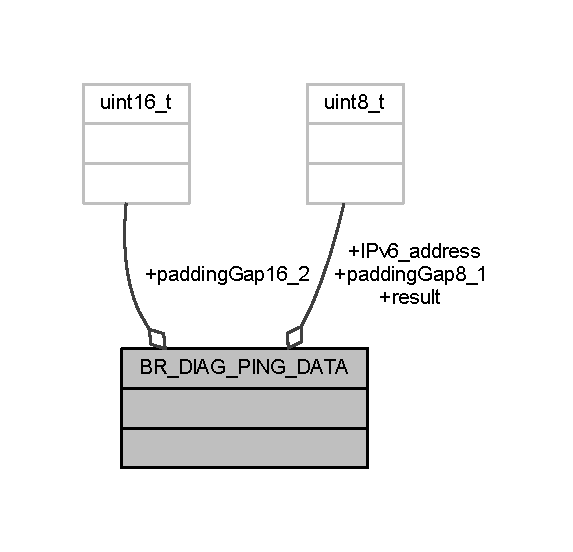
\includegraphics[width=275pt]{struct_b_r___d_i_a_g___p_i_n_g___d_a_t_a__coll__graph}
\end{center}
\end{figure}
\subsection*{Public Attributes}
\begin{DoxyCompactItemize}
\item 
uint8\+\_\+t \mbox{\hyperlink{struct_b_r___d_i_a_g___p_i_n_g___d_a_t_a_ab2996a088cc43e9ab39b5d108d95682f}{I\+Pv6\+\_\+address}} \mbox{[}16\mbox{]}
\item 
uint8\+\_\+t \mbox{\hyperlink{struct_b_r___d_i_a_g___p_i_n_g___d_a_t_a_ac31c42bf1a1783d9c6aa3de70a0b29cf}{result}}
\item 
uint8\+\_\+t \mbox{\hyperlink{struct_b_r___d_i_a_g___p_i_n_g___d_a_t_a_a232a176e3dad7eaba4dfc978610042e8}{padding\+Gap8\+\_\+1}}
\item 
uint16\+\_\+t \mbox{\hyperlink{struct_b_r___d_i_a_g___p_i_n_g___d_a_t_a_a1c4c77e6f2aabcaec588628a55a25bed}{padding\+Gap16\+\_\+2}}
\end{DoxyCompactItemize}


\subsection{Member Data Documentation}
\mbox{\Hypertarget{struct_b_r___d_i_a_g___p_i_n_g___d_a_t_a_ab2996a088cc43e9ab39b5d108d95682f}\label{struct_b_r___d_i_a_g___p_i_n_g___d_a_t_a_ab2996a088cc43e9ab39b5d108d95682f}} 
\index{B\+R\+\_\+\+D\+I\+A\+G\+\_\+\+P\+I\+N\+G\+\_\+\+D\+A\+TA@{B\+R\+\_\+\+D\+I\+A\+G\+\_\+\+P\+I\+N\+G\+\_\+\+D\+A\+TA}!I\+Pv6\+\_\+address@{I\+Pv6\+\_\+address}}
\index{I\+Pv6\+\_\+address@{I\+Pv6\+\_\+address}!B\+R\+\_\+\+D\+I\+A\+G\+\_\+\+P\+I\+N\+G\+\_\+\+D\+A\+TA@{B\+R\+\_\+\+D\+I\+A\+G\+\_\+\+P\+I\+N\+G\+\_\+\+D\+A\+TA}}
\subsubsection{\texorpdfstring{I\+Pv6\+\_\+address}{IPv6\_address}}
{\footnotesize\ttfamily uint8\+\_\+t B\+R\+\_\+\+D\+I\+A\+G\+\_\+\+P\+I\+N\+G\+\_\+\+D\+A\+T\+A\+::\+I\+Pv6\+\_\+address\mbox{[}16\mbox{]}}

\mbox{\Hypertarget{struct_b_r___d_i_a_g___p_i_n_g___d_a_t_a_a1c4c77e6f2aabcaec588628a55a25bed}\label{struct_b_r___d_i_a_g___p_i_n_g___d_a_t_a_a1c4c77e6f2aabcaec588628a55a25bed}} 
\index{B\+R\+\_\+\+D\+I\+A\+G\+\_\+\+P\+I\+N\+G\+\_\+\+D\+A\+TA@{B\+R\+\_\+\+D\+I\+A\+G\+\_\+\+P\+I\+N\+G\+\_\+\+D\+A\+TA}!padding\+Gap16\+\_\+2@{padding\+Gap16\+\_\+2}}
\index{padding\+Gap16\+\_\+2@{padding\+Gap16\+\_\+2}!B\+R\+\_\+\+D\+I\+A\+G\+\_\+\+P\+I\+N\+G\+\_\+\+D\+A\+TA@{B\+R\+\_\+\+D\+I\+A\+G\+\_\+\+P\+I\+N\+G\+\_\+\+D\+A\+TA}}
\subsubsection{\texorpdfstring{padding\+Gap16\+\_\+2}{paddingGap16\_2}}
{\footnotesize\ttfamily uint16\+\_\+t B\+R\+\_\+\+D\+I\+A\+G\+\_\+\+P\+I\+N\+G\+\_\+\+D\+A\+T\+A\+::padding\+Gap16\+\_\+2}

\mbox{\Hypertarget{struct_b_r___d_i_a_g___p_i_n_g___d_a_t_a_a232a176e3dad7eaba4dfc978610042e8}\label{struct_b_r___d_i_a_g___p_i_n_g___d_a_t_a_a232a176e3dad7eaba4dfc978610042e8}} 
\index{B\+R\+\_\+\+D\+I\+A\+G\+\_\+\+P\+I\+N\+G\+\_\+\+D\+A\+TA@{B\+R\+\_\+\+D\+I\+A\+G\+\_\+\+P\+I\+N\+G\+\_\+\+D\+A\+TA}!padding\+Gap8\+\_\+1@{padding\+Gap8\+\_\+1}}
\index{padding\+Gap8\+\_\+1@{padding\+Gap8\+\_\+1}!B\+R\+\_\+\+D\+I\+A\+G\+\_\+\+P\+I\+N\+G\+\_\+\+D\+A\+TA@{B\+R\+\_\+\+D\+I\+A\+G\+\_\+\+P\+I\+N\+G\+\_\+\+D\+A\+TA}}
\subsubsection{\texorpdfstring{padding\+Gap8\+\_\+1}{paddingGap8\_1}}
{\footnotesize\ttfamily uint8\+\_\+t B\+R\+\_\+\+D\+I\+A\+G\+\_\+\+P\+I\+N\+G\+\_\+\+D\+A\+T\+A\+::padding\+Gap8\+\_\+1}

\mbox{\Hypertarget{struct_b_r___d_i_a_g___p_i_n_g___d_a_t_a_ac31c42bf1a1783d9c6aa3de70a0b29cf}\label{struct_b_r___d_i_a_g___p_i_n_g___d_a_t_a_ac31c42bf1a1783d9c6aa3de70a0b29cf}} 
\index{B\+R\+\_\+\+D\+I\+A\+G\+\_\+\+P\+I\+N\+G\+\_\+\+D\+A\+TA@{B\+R\+\_\+\+D\+I\+A\+G\+\_\+\+P\+I\+N\+G\+\_\+\+D\+A\+TA}!result@{result}}
\index{result@{result}!B\+R\+\_\+\+D\+I\+A\+G\+\_\+\+P\+I\+N\+G\+\_\+\+D\+A\+TA@{B\+R\+\_\+\+D\+I\+A\+G\+\_\+\+P\+I\+N\+G\+\_\+\+D\+A\+TA}}
\subsubsection{\texorpdfstring{result}{result}}
{\footnotesize\ttfamily uint8\+\_\+t B\+R\+\_\+\+D\+I\+A\+G\+\_\+\+P\+I\+N\+G\+\_\+\+D\+A\+T\+A\+::result}



The documentation for this struct was generated from the following file\+:\begin{DoxyCompactItemize}
\item 
\mbox{\hyperlink{tttech_broad_r_reach_8h}{tttech\+Broad\+R\+Reach.\+h}}\end{DoxyCompactItemize}

\hypertarget{struct_b_r___info}{}\section{B\+R\+\_\+\+Info Struct Reference}
\label{struct_b_r___info}\index{B\+R\+\_\+\+Info@{B\+R\+\_\+\+Info}}


description  




{\ttfamily \#include $<$tttech\+Broad\+R\+Reach.\+h$>$}



Collaboration diagram for B\+R\+\_\+\+Info\+:\nopagebreak
\begin{figure}[H]
\begin{center}
\leavevmode
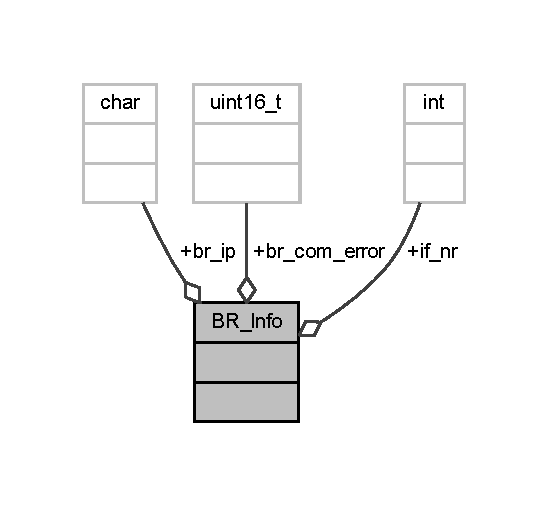
\includegraphics[width=263pt]{struct_b_r___info__coll__graph}
\end{center}
\end{figure}
\subsection*{Public Attributes}
\begin{DoxyCompactItemize}
\item 
int \mbox{\hyperlink{struct_b_r___info_ad3139482d149e41ec15ac355cf4d5251}{if\+\_\+nr}}
\item 
uint16\+\_\+t \mbox{\hyperlink{struct_b_r___info_ac3670b53bfa902bb4295495b61fb6985}{br\+\_\+com\+\_\+error}}
\item 
char \mbox{\hyperlink{struct_b_r___info_a8923532471f4ec953142656d0414765f}{br\+\_\+ip}} \mbox{[}46\mbox{]}
\end{DoxyCompactItemize}


\subsection{Detailed Description}
description 

\subsection{Member Data Documentation}
\mbox{\Hypertarget{struct_b_r___info_ac3670b53bfa902bb4295495b61fb6985}\label{struct_b_r___info_ac3670b53bfa902bb4295495b61fb6985}} 
\index{B\+R\+\_\+\+Info@{B\+R\+\_\+\+Info}!br\+\_\+com\+\_\+error@{br\+\_\+com\+\_\+error}}
\index{br\+\_\+com\+\_\+error@{br\+\_\+com\+\_\+error}!B\+R\+\_\+\+Info@{B\+R\+\_\+\+Info}}
\subsubsection{\texorpdfstring{br\+\_\+com\+\_\+error}{br\_com\_error}}
{\footnotesize\ttfamily uint16\+\_\+t B\+R\+\_\+\+Info\+::br\+\_\+com\+\_\+error}

\mbox{\Hypertarget{struct_b_r___info_a8923532471f4ec953142656d0414765f}\label{struct_b_r___info_a8923532471f4ec953142656d0414765f}} 
\index{B\+R\+\_\+\+Info@{B\+R\+\_\+\+Info}!br\+\_\+ip@{br\+\_\+ip}}
\index{br\+\_\+ip@{br\+\_\+ip}!B\+R\+\_\+\+Info@{B\+R\+\_\+\+Info}}
\subsubsection{\texorpdfstring{br\+\_\+ip}{br\_ip}}
{\footnotesize\ttfamily char B\+R\+\_\+\+Info\+::br\+\_\+ip\mbox{[}46\mbox{]}}

\mbox{\Hypertarget{struct_b_r___info_ad3139482d149e41ec15ac355cf4d5251}\label{struct_b_r___info_ad3139482d149e41ec15ac355cf4d5251}} 
\index{B\+R\+\_\+\+Info@{B\+R\+\_\+\+Info}!if\+\_\+nr@{if\+\_\+nr}}
\index{if\+\_\+nr@{if\+\_\+nr}!B\+R\+\_\+\+Info@{B\+R\+\_\+\+Info}}
\subsubsection{\texorpdfstring{if\+\_\+nr}{if\_nr}}
{\footnotesize\ttfamily int B\+R\+\_\+\+Info\+::if\+\_\+nr}



The documentation for this struct was generated from the following file\+:\begin{DoxyCompactItemize}
\item 
\mbox{\hyperlink{tttech_broad_r_reach_8h}{tttech\+Broad\+R\+Reach.\+h}}\end{DoxyCompactItemize}

\hypertarget{struct_b_r_diag_data}{}\section{B\+R\+Diag\+Data Struct Reference}
\label{struct_b_r_diag_data}\index{B\+R\+Diag\+Data@{B\+R\+Diag\+Data}}


description  




{\ttfamily \#include $<$tttech\+Broad\+R\+Reach.\+h$>$}



Collaboration diagram for B\+R\+Diag\+Data\+:
\nopagebreak
\begin{figure}[H]
\begin{center}
\leavevmode
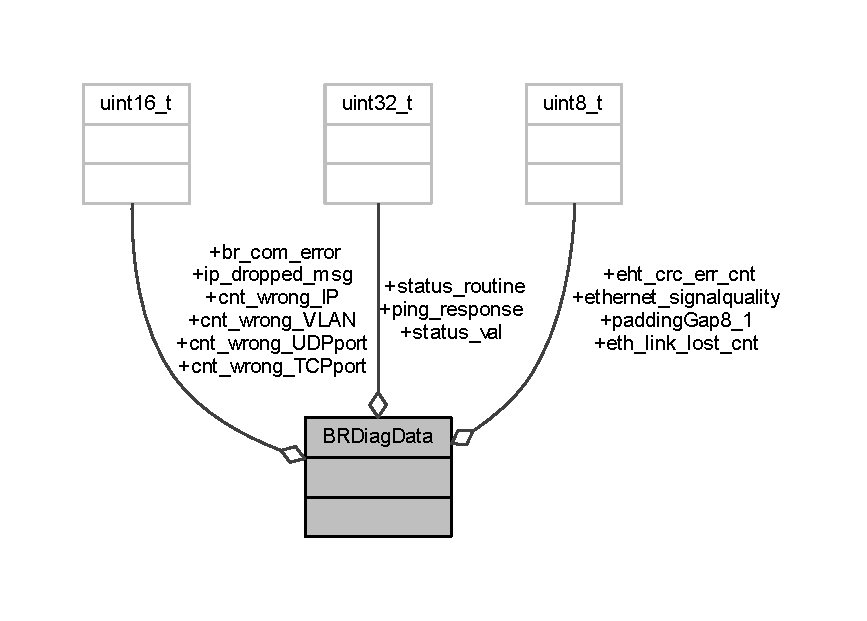
\includegraphics[width=350pt]{struct_b_r_diag_data__coll__graph}
\end{center}
\end{figure}
\subsection*{Public Attributes}
\begin{DoxyCompactItemize}
\item 
uint32\+\_\+t \mbox{\hyperlink{struct_b_r_diag_data_a29727be81df0a5cab888e7c16c78f152}{status\+\_\+routine}}
\item 
uint32\+\_\+t \mbox{\hyperlink{struct_b_r_diag_data_a1b6c0080fff5bddfc534cf9b50d52564}{status\+\_\+val}}
\item 
uint32\+\_\+t \mbox{\hyperlink{struct_b_r_diag_data_a525c855c97fe37dd7447ac2890bb4842}{ping\+\_\+response}}
\item 
uint16\+\_\+t \mbox{\hyperlink{struct_b_r_diag_data_a52ec83c444fe23cc253d2a7b5d788326}{br\+\_\+com\+\_\+error}}
\item 
uint16\+\_\+t \mbox{\hyperlink{struct_b_r_diag_data_acc7b07f207627a8b156283e88d4c7a8e}{ip\+\_\+dropped\+\_\+msg}}
\item 
uint16\+\_\+t \mbox{\hyperlink{struct_b_r_diag_data_a12d116dc3607d10fe1e772435a064857}{cnt\+\_\+wrong\+\_\+\+V\+L\+AN}}
\item 
uint16\+\_\+t \mbox{\hyperlink{struct_b_r_diag_data_a547b4cf3fcd1d5686591da312e375e21}{cnt\+\_\+wrong\+\_\+\+IP}}
\item 
uint16\+\_\+t \mbox{\hyperlink{struct_b_r_diag_data_acfd5368dd58e132b13062dbad9ae2dd8}{cnt\+\_\+wrong\+\_\+\+T\+C\+Pport}}
\item 
uint16\+\_\+t \mbox{\hyperlink{struct_b_r_diag_data_a5835a6a7161d695e1724da1ce9185339}{cnt\+\_\+wrong\+\_\+\+U\+D\+Pport}}
\item 
uint8\+\_\+t \mbox{\hyperlink{struct_b_r_diag_data_a857fefa87840d357d7bb5f2ae82fe25f}{ethernet\+\_\+signalquality}}
\item 
uint8\+\_\+t \mbox{\hyperlink{struct_b_r_diag_data_a39130c14ab5e3e3b638b7ece79b1eadc}{eth\+\_\+link\+\_\+lost\+\_\+cnt}}
\item 
uint8\+\_\+t \mbox{\hyperlink{struct_b_r_diag_data_a2b044ae057e4dd84e91ef6a73ccb9053}{eht\+\_\+crc\+\_\+err\+\_\+cnt}}
\item 
uint8\+\_\+t \mbox{\hyperlink{struct_b_r_diag_data_ad21747ff95da8debf8e9c0bc1c4fcd44}{padding\+Gap8\+\_\+1}}
\end{DoxyCompactItemize}


\subsection{Detailed Description}
description 

\subsection{Member Data Documentation}
\mbox{\Hypertarget{struct_b_r_diag_data_a52ec83c444fe23cc253d2a7b5d788326}\label{struct_b_r_diag_data_a52ec83c444fe23cc253d2a7b5d788326}} 
\index{B\+R\+Diag\+Data@{B\+R\+Diag\+Data}!br\+\_\+com\+\_\+error@{br\+\_\+com\+\_\+error}}
\index{br\+\_\+com\+\_\+error@{br\+\_\+com\+\_\+error}!B\+R\+Diag\+Data@{B\+R\+Diag\+Data}}
\subsubsection{\texorpdfstring{br\+\_\+com\+\_\+error}{br\_com\_error}}
{\footnotesize\ttfamily uint16\+\_\+t B\+R\+Diag\+Data\+::br\+\_\+com\+\_\+error}

\mbox{\Hypertarget{struct_b_r_diag_data_a547b4cf3fcd1d5686591da312e375e21}\label{struct_b_r_diag_data_a547b4cf3fcd1d5686591da312e375e21}} 
\index{B\+R\+Diag\+Data@{B\+R\+Diag\+Data}!cnt\+\_\+wrong\+\_\+\+IP@{cnt\+\_\+wrong\+\_\+\+IP}}
\index{cnt\+\_\+wrong\+\_\+\+IP@{cnt\+\_\+wrong\+\_\+\+IP}!B\+R\+Diag\+Data@{B\+R\+Diag\+Data}}
\subsubsection{\texorpdfstring{cnt\+\_\+wrong\+\_\+\+IP}{cnt\_wrong\_IP}}
{\footnotesize\ttfamily uint16\+\_\+t B\+R\+Diag\+Data\+::cnt\+\_\+wrong\+\_\+\+IP}

\mbox{\Hypertarget{struct_b_r_diag_data_acfd5368dd58e132b13062dbad9ae2dd8}\label{struct_b_r_diag_data_acfd5368dd58e132b13062dbad9ae2dd8}} 
\index{B\+R\+Diag\+Data@{B\+R\+Diag\+Data}!cnt\+\_\+wrong\+\_\+\+T\+C\+Pport@{cnt\+\_\+wrong\+\_\+\+T\+C\+Pport}}
\index{cnt\+\_\+wrong\+\_\+\+T\+C\+Pport@{cnt\+\_\+wrong\+\_\+\+T\+C\+Pport}!B\+R\+Diag\+Data@{B\+R\+Diag\+Data}}
\subsubsection{\texorpdfstring{cnt\+\_\+wrong\+\_\+\+T\+C\+Pport}{cnt\_wrong\_TCPport}}
{\footnotesize\ttfamily uint16\+\_\+t B\+R\+Diag\+Data\+::cnt\+\_\+wrong\+\_\+\+T\+C\+Pport}

\mbox{\Hypertarget{struct_b_r_diag_data_a5835a6a7161d695e1724da1ce9185339}\label{struct_b_r_diag_data_a5835a6a7161d695e1724da1ce9185339}} 
\index{B\+R\+Diag\+Data@{B\+R\+Diag\+Data}!cnt\+\_\+wrong\+\_\+\+U\+D\+Pport@{cnt\+\_\+wrong\+\_\+\+U\+D\+Pport}}
\index{cnt\+\_\+wrong\+\_\+\+U\+D\+Pport@{cnt\+\_\+wrong\+\_\+\+U\+D\+Pport}!B\+R\+Diag\+Data@{B\+R\+Diag\+Data}}
\subsubsection{\texorpdfstring{cnt\+\_\+wrong\+\_\+\+U\+D\+Pport}{cnt\_wrong\_UDPport}}
{\footnotesize\ttfamily uint16\+\_\+t B\+R\+Diag\+Data\+::cnt\+\_\+wrong\+\_\+\+U\+D\+Pport}

\mbox{\Hypertarget{struct_b_r_diag_data_a12d116dc3607d10fe1e772435a064857}\label{struct_b_r_diag_data_a12d116dc3607d10fe1e772435a064857}} 
\index{B\+R\+Diag\+Data@{B\+R\+Diag\+Data}!cnt\+\_\+wrong\+\_\+\+V\+L\+AN@{cnt\+\_\+wrong\+\_\+\+V\+L\+AN}}
\index{cnt\+\_\+wrong\+\_\+\+V\+L\+AN@{cnt\+\_\+wrong\+\_\+\+V\+L\+AN}!B\+R\+Diag\+Data@{B\+R\+Diag\+Data}}
\subsubsection{\texorpdfstring{cnt\+\_\+wrong\+\_\+\+V\+L\+AN}{cnt\_wrong\_VLAN}}
{\footnotesize\ttfamily uint16\+\_\+t B\+R\+Diag\+Data\+::cnt\+\_\+wrong\+\_\+\+V\+L\+AN}

\mbox{\Hypertarget{struct_b_r_diag_data_a2b044ae057e4dd84e91ef6a73ccb9053}\label{struct_b_r_diag_data_a2b044ae057e4dd84e91ef6a73ccb9053}} 
\index{B\+R\+Diag\+Data@{B\+R\+Diag\+Data}!eht\+\_\+crc\+\_\+err\+\_\+cnt@{eht\+\_\+crc\+\_\+err\+\_\+cnt}}
\index{eht\+\_\+crc\+\_\+err\+\_\+cnt@{eht\+\_\+crc\+\_\+err\+\_\+cnt}!B\+R\+Diag\+Data@{B\+R\+Diag\+Data}}
\subsubsection{\texorpdfstring{eht\+\_\+crc\+\_\+err\+\_\+cnt}{eht\_crc\_err\_cnt}}
{\footnotesize\ttfamily uint8\+\_\+t B\+R\+Diag\+Data\+::eht\+\_\+crc\+\_\+err\+\_\+cnt}

\mbox{\Hypertarget{struct_b_r_diag_data_a39130c14ab5e3e3b638b7ece79b1eadc}\label{struct_b_r_diag_data_a39130c14ab5e3e3b638b7ece79b1eadc}} 
\index{B\+R\+Diag\+Data@{B\+R\+Diag\+Data}!eth\+\_\+link\+\_\+lost\+\_\+cnt@{eth\+\_\+link\+\_\+lost\+\_\+cnt}}
\index{eth\+\_\+link\+\_\+lost\+\_\+cnt@{eth\+\_\+link\+\_\+lost\+\_\+cnt}!B\+R\+Diag\+Data@{B\+R\+Diag\+Data}}
\subsubsection{\texorpdfstring{eth\+\_\+link\+\_\+lost\+\_\+cnt}{eth\_link\_lost\_cnt}}
{\footnotesize\ttfamily uint8\+\_\+t B\+R\+Diag\+Data\+::eth\+\_\+link\+\_\+lost\+\_\+cnt}

\mbox{\Hypertarget{struct_b_r_diag_data_a857fefa87840d357d7bb5f2ae82fe25f}\label{struct_b_r_diag_data_a857fefa87840d357d7bb5f2ae82fe25f}} 
\index{B\+R\+Diag\+Data@{B\+R\+Diag\+Data}!ethernet\+\_\+signalquality@{ethernet\+\_\+signalquality}}
\index{ethernet\+\_\+signalquality@{ethernet\+\_\+signalquality}!B\+R\+Diag\+Data@{B\+R\+Diag\+Data}}
\subsubsection{\texorpdfstring{ethernet\+\_\+signalquality}{ethernet\_signalquality}}
{\footnotesize\ttfamily uint8\+\_\+t B\+R\+Diag\+Data\+::ethernet\+\_\+signalquality}

\mbox{\Hypertarget{struct_b_r_diag_data_acc7b07f207627a8b156283e88d4c7a8e}\label{struct_b_r_diag_data_acc7b07f207627a8b156283e88d4c7a8e}} 
\index{B\+R\+Diag\+Data@{B\+R\+Diag\+Data}!ip\+\_\+dropped\+\_\+msg@{ip\+\_\+dropped\+\_\+msg}}
\index{ip\+\_\+dropped\+\_\+msg@{ip\+\_\+dropped\+\_\+msg}!B\+R\+Diag\+Data@{B\+R\+Diag\+Data}}
\subsubsection{\texorpdfstring{ip\+\_\+dropped\+\_\+msg}{ip\_dropped\_msg}}
{\footnotesize\ttfamily uint16\+\_\+t B\+R\+Diag\+Data\+::ip\+\_\+dropped\+\_\+msg}

\mbox{\Hypertarget{struct_b_r_diag_data_ad21747ff95da8debf8e9c0bc1c4fcd44}\label{struct_b_r_diag_data_ad21747ff95da8debf8e9c0bc1c4fcd44}} 
\index{B\+R\+Diag\+Data@{B\+R\+Diag\+Data}!padding\+Gap8\+\_\+1@{padding\+Gap8\+\_\+1}}
\index{padding\+Gap8\+\_\+1@{padding\+Gap8\+\_\+1}!B\+R\+Diag\+Data@{B\+R\+Diag\+Data}}
\subsubsection{\texorpdfstring{padding\+Gap8\+\_\+1}{paddingGap8\_1}}
{\footnotesize\ttfamily uint8\+\_\+t B\+R\+Diag\+Data\+::padding\+Gap8\+\_\+1}

\mbox{\Hypertarget{struct_b_r_diag_data_a525c855c97fe37dd7447ac2890bb4842}\label{struct_b_r_diag_data_a525c855c97fe37dd7447ac2890bb4842}} 
\index{B\+R\+Diag\+Data@{B\+R\+Diag\+Data}!ping\+\_\+response@{ping\+\_\+response}}
\index{ping\+\_\+response@{ping\+\_\+response}!B\+R\+Diag\+Data@{B\+R\+Diag\+Data}}
\subsubsection{\texorpdfstring{ping\+\_\+response}{ping\_response}}
{\footnotesize\ttfamily uint32\+\_\+t B\+R\+Diag\+Data\+::ping\+\_\+response}

\mbox{\Hypertarget{struct_b_r_diag_data_a29727be81df0a5cab888e7c16c78f152}\label{struct_b_r_diag_data_a29727be81df0a5cab888e7c16c78f152}} 
\index{B\+R\+Diag\+Data@{B\+R\+Diag\+Data}!status\+\_\+routine@{status\+\_\+routine}}
\index{status\+\_\+routine@{status\+\_\+routine}!B\+R\+Diag\+Data@{B\+R\+Diag\+Data}}
\subsubsection{\texorpdfstring{status\+\_\+routine}{status\_routine}}
{\footnotesize\ttfamily uint32\+\_\+t B\+R\+Diag\+Data\+::status\+\_\+routine}

\mbox{\Hypertarget{struct_b_r_diag_data_a1b6c0080fff5bddfc534cf9b50d52564}\label{struct_b_r_diag_data_a1b6c0080fff5bddfc534cf9b50d52564}} 
\index{B\+R\+Diag\+Data@{B\+R\+Diag\+Data}!status\+\_\+val@{status\+\_\+val}}
\index{status\+\_\+val@{status\+\_\+val}!B\+R\+Diag\+Data@{B\+R\+Diag\+Data}}
\subsubsection{\texorpdfstring{status\+\_\+val}{status\_val}}
{\footnotesize\ttfamily uint32\+\_\+t B\+R\+Diag\+Data\+::status\+\_\+val}



The documentation for this struct was generated from the following file\+:\begin{DoxyCompactItemize}
\item 
\mbox{\hyperlink{tttech_broad_r_reach_8h}{tttech\+Broad\+R\+Reach.\+h}}\end{DoxyCompactItemize}

\hypertarget{structdiagnostic_data_msg_q}{}\section{diagnostic\+Data\+MsgQ Struct Reference}
\label{structdiagnostic_data_msg_q}\index{diagnostic\+Data\+MsgQ@{diagnostic\+Data\+MsgQ}}


{\ttfamily \#include $<$module\+One\+Read\+Eth\+Phy.\+h$>$}



Collaboration diagram for diagnostic\+Data\+MsgQ\+:
\nopagebreak
\begin{figure}[H]
\begin{center}
\leavevmode
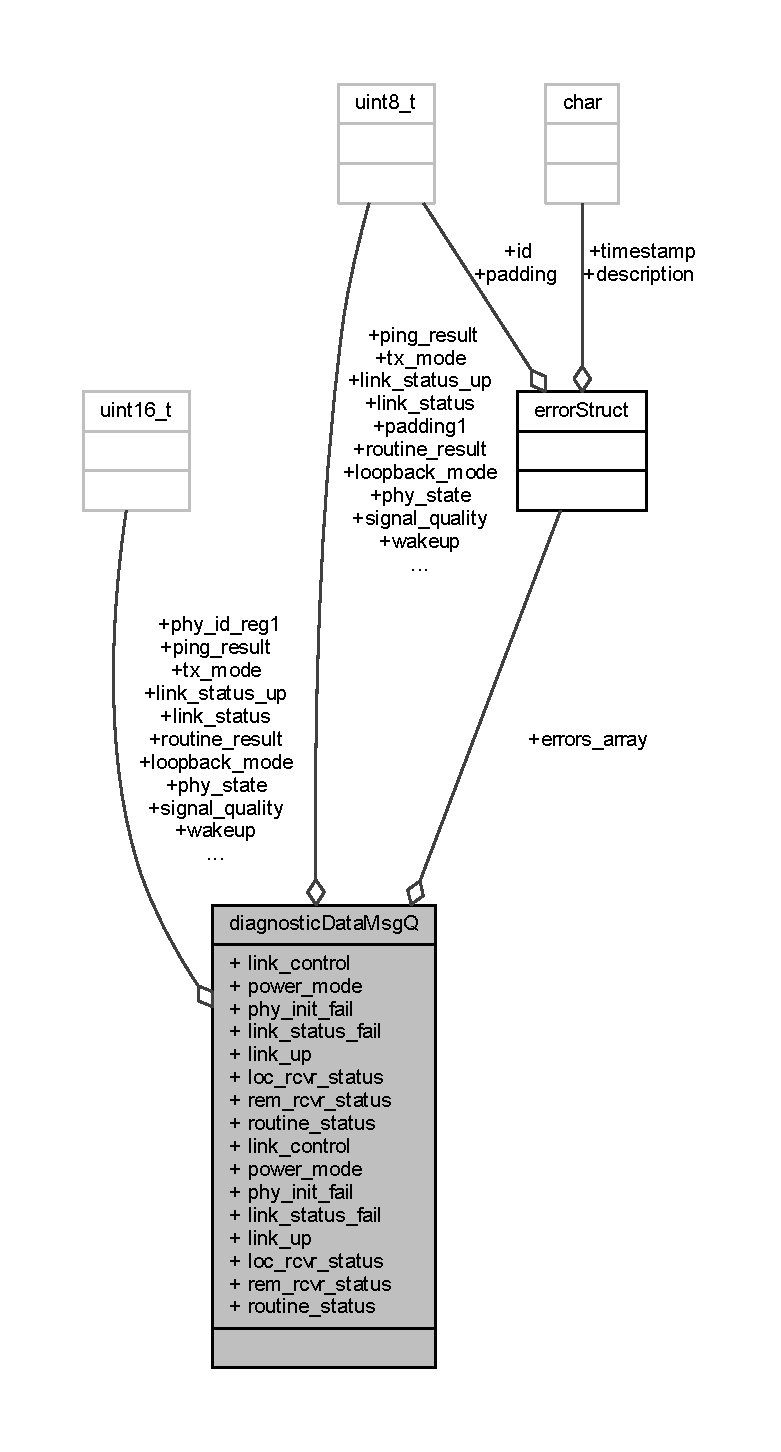
\includegraphics[width=350pt]{structdiagnostic_data_msg_q__coll__graph}
\end{center}
\end{figure}
\subsection*{Public Attributes}
\begin{DoxyCompactItemize}
\item 
uint8\+\_\+t \mbox{\hyperlink{structdiagnostic_data_msg_q_a1a712ef6bb1c0029592c3dbafa31a569}{link\+\_\+status}}
\item 
uint8\+\_\+t \mbox{\hyperlink{structdiagnostic_data_msg_q_a955326ea4924202ca8e42d37aec42532}{link\+\_\+control}}
\item 
uint8\+\_\+t \mbox{\hyperlink{structdiagnostic_data_msg_q_a67e41bd75ee9bd90fa84aed31f3b20ce}{power\+\_\+mode}}
\item 
uint8\+\_\+t \mbox{\hyperlink{structdiagnostic_data_msg_q_a71457503c7539ee6ca5936caf7acbcba}{loopback\+\_\+mode}}
\item 
uint8\+\_\+t \mbox{\hyperlink{structdiagnostic_data_msg_q_a598c0800fea8295ec1f61e06632e45b9}{phy\+\_\+init\+\_\+fail}}
\item 
uint8\+\_\+t \mbox{\hyperlink{structdiagnostic_data_msg_q_a1dc3ed269a7173a68e81cf00a13ed0d3}{wakeup}}
\item 
uint8\+\_\+t \mbox{\hyperlink{structdiagnostic_data_msg_q_acc605c651f6942c37e70b55dd5f44ed6}{link\+\_\+status\+\_\+fail}}
\item 
uint8\+\_\+t \mbox{\hyperlink{structdiagnostic_data_msg_q_a00ca8cdfc103ff49d8f36be6a211d272}{link\+\_\+status\+\_\+up}}
\item 
uint8\+\_\+t \mbox{\hyperlink{structdiagnostic_data_msg_q_a4c8067ddcba243b029bafb045f19e273}{link\+\_\+up}}
\item 
uint8\+\_\+t \mbox{\hyperlink{structdiagnostic_data_msg_q_abc446ab4a822dc4fba0cbb6d3f5b234c}{tx\+\_\+mode}}
\item 
uint8\+\_\+t \mbox{\hyperlink{structdiagnostic_data_msg_q_ad74c875c8d081aad08753989f143b439}{loc\+\_\+rcvr\+\_\+status}}
\item 
uint8\+\_\+t \mbox{\hyperlink{structdiagnostic_data_msg_q_a8b26cfb36423cac2f1f66ef21217f089}{rem\+\_\+rcvr\+\_\+status}}
\item 
uint8\+\_\+t \mbox{\hyperlink{structdiagnostic_data_msg_q_a2cbee01deb307a445abc8ef0dfdd56f3}{signal\+\_\+quality}}
\item 
uint16\+\_\+t \mbox{\hyperlink{structdiagnostic_data_msg_q_ad301b21bba0db0dae4edcee06ea102af}{phy\+\_\+id\+\_\+reg1}}
\item 
uint8\+\_\+t \mbox{\hyperlink{structdiagnostic_data_msg_q_a63f0f4136d1628b267af0afc1c6df9cf}{phy\+\_\+state}}
\item 
uint8\+\_\+t \mbox{\hyperlink{structdiagnostic_data_msg_q_aa267ac90c45771daeeee3eec5e51abf2}{ping\+\_\+result}}
\item 
uint8\+\_\+t \mbox{\hyperlink{structdiagnostic_data_msg_q_a549e1a6a2eecb5b966b5a10c6274ccf3}{routine\+\_\+status}}
\item 
uint8\+\_\+t \mbox{\hyperlink{structdiagnostic_data_msg_q_a66ad8d88474dbe4840efe79f4a071efd}{routine\+\_\+result}}
\item 
\mbox{\hyperlink{module_one_read_eth_phy_8h_a20a1de38f8a31b563f5185bf73d836b0}{s\+\_\+\+E\+R\+R\+O\+RS}} \mbox{\hyperlink{structdiagnostic_data_msg_q_a70a56a13a2c9f8f28679b51484db2557}{errors\+\_\+array}} \mbox{[}4\mbox{]}
\item 
uint8\+\_\+t \mbox{\hyperlink{structdiagnostic_data_msg_q_aa5156e3e0221275658d1bdfd3d2299bb}{padding1}}
\end{DoxyCompactItemize}


\subsection{Member Data Documentation}
\mbox{\Hypertarget{structdiagnostic_data_msg_q_a70a56a13a2c9f8f28679b51484db2557}\label{structdiagnostic_data_msg_q_a70a56a13a2c9f8f28679b51484db2557}} 
\index{diagnostic\+Data\+MsgQ@{diagnostic\+Data\+MsgQ}!errors\+\_\+array@{errors\+\_\+array}}
\index{errors\+\_\+array@{errors\+\_\+array}!diagnostic\+Data\+MsgQ@{diagnostic\+Data\+MsgQ}}
\subsubsection{\texorpdfstring{errors\+\_\+array}{errors\_array}}
{\footnotesize\ttfamily \mbox{\hyperlink{module_one_read_eth_phy_8h_a20a1de38f8a31b563f5185bf73d836b0}{s\+\_\+\+E\+R\+R\+O\+RS}} diagnostic\+Data\+Msg\+Q\+::errors\+\_\+array}

\mbox{\Hypertarget{structdiagnostic_data_msg_q_a955326ea4924202ca8e42d37aec42532}\label{structdiagnostic_data_msg_q_a955326ea4924202ca8e42d37aec42532}} 
\index{diagnostic\+Data\+MsgQ@{diagnostic\+Data\+MsgQ}!link\+\_\+control@{link\+\_\+control}}
\index{link\+\_\+control@{link\+\_\+control}!diagnostic\+Data\+MsgQ@{diagnostic\+Data\+MsgQ}}
\subsubsection{\texorpdfstring{link\+\_\+control}{link\_control}}
{\footnotesize\ttfamily uint8\+\_\+t diagnostic\+Data\+Msg\+Q\+::link\+\_\+control}

\mbox{\Hypertarget{structdiagnostic_data_msg_q_a1a712ef6bb1c0029592c3dbafa31a569}\label{structdiagnostic_data_msg_q_a1a712ef6bb1c0029592c3dbafa31a569}} 
\index{diagnostic\+Data\+MsgQ@{diagnostic\+Data\+MsgQ}!link\+\_\+status@{link\+\_\+status}}
\index{link\+\_\+status@{link\+\_\+status}!diagnostic\+Data\+MsgQ@{diagnostic\+Data\+MsgQ}}
\subsubsection{\texorpdfstring{link\+\_\+status}{link\_status}}
{\footnotesize\ttfamily uint8\+\_\+t diagnostic\+Data\+Msg\+Q\+::link\+\_\+status}

\mbox{\Hypertarget{structdiagnostic_data_msg_q_acc605c651f6942c37e70b55dd5f44ed6}\label{structdiagnostic_data_msg_q_acc605c651f6942c37e70b55dd5f44ed6}} 
\index{diagnostic\+Data\+MsgQ@{diagnostic\+Data\+MsgQ}!link\+\_\+status\+\_\+fail@{link\+\_\+status\+\_\+fail}}
\index{link\+\_\+status\+\_\+fail@{link\+\_\+status\+\_\+fail}!diagnostic\+Data\+MsgQ@{diagnostic\+Data\+MsgQ}}
\subsubsection{\texorpdfstring{link\+\_\+status\+\_\+fail}{link\_status\_fail}}
{\footnotesize\ttfamily uint8\+\_\+t diagnostic\+Data\+Msg\+Q\+::link\+\_\+status\+\_\+fail}

\mbox{\Hypertarget{structdiagnostic_data_msg_q_a00ca8cdfc103ff49d8f36be6a211d272}\label{structdiagnostic_data_msg_q_a00ca8cdfc103ff49d8f36be6a211d272}} 
\index{diagnostic\+Data\+MsgQ@{diagnostic\+Data\+MsgQ}!link\+\_\+status\+\_\+up@{link\+\_\+status\+\_\+up}}
\index{link\+\_\+status\+\_\+up@{link\+\_\+status\+\_\+up}!diagnostic\+Data\+MsgQ@{diagnostic\+Data\+MsgQ}}
\subsubsection{\texorpdfstring{link\+\_\+status\+\_\+up}{link\_status\_up}}
{\footnotesize\ttfamily uint8\+\_\+t diagnostic\+Data\+Msg\+Q\+::link\+\_\+status\+\_\+up}

\mbox{\Hypertarget{structdiagnostic_data_msg_q_a4c8067ddcba243b029bafb045f19e273}\label{structdiagnostic_data_msg_q_a4c8067ddcba243b029bafb045f19e273}} 
\index{diagnostic\+Data\+MsgQ@{diagnostic\+Data\+MsgQ}!link\+\_\+up@{link\+\_\+up}}
\index{link\+\_\+up@{link\+\_\+up}!diagnostic\+Data\+MsgQ@{diagnostic\+Data\+MsgQ}}
\subsubsection{\texorpdfstring{link\+\_\+up}{link\_up}}
{\footnotesize\ttfamily uint8\+\_\+t diagnostic\+Data\+Msg\+Q\+::link\+\_\+up}

\mbox{\Hypertarget{structdiagnostic_data_msg_q_ad74c875c8d081aad08753989f143b439}\label{structdiagnostic_data_msg_q_ad74c875c8d081aad08753989f143b439}} 
\index{diagnostic\+Data\+MsgQ@{diagnostic\+Data\+MsgQ}!loc\+\_\+rcvr\+\_\+status@{loc\+\_\+rcvr\+\_\+status}}
\index{loc\+\_\+rcvr\+\_\+status@{loc\+\_\+rcvr\+\_\+status}!diagnostic\+Data\+MsgQ@{diagnostic\+Data\+MsgQ}}
\subsubsection{\texorpdfstring{loc\+\_\+rcvr\+\_\+status}{loc\_rcvr\_status}}
{\footnotesize\ttfamily uint8\+\_\+t diagnostic\+Data\+Msg\+Q\+::loc\+\_\+rcvr\+\_\+status}

\mbox{\Hypertarget{structdiagnostic_data_msg_q_a71457503c7539ee6ca5936caf7acbcba}\label{structdiagnostic_data_msg_q_a71457503c7539ee6ca5936caf7acbcba}} 
\index{diagnostic\+Data\+MsgQ@{diagnostic\+Data\+MsgQ}!loopback\+\_\+mode@{loopback\+\_\+mode}}
\index{loopback\+\_\+mode@{loopback\+\_\+mode}!diagnostic\+Data\+MsgQ@{diagnostic\+Data\+MsgQ}}
\subsubsection{\texorpdfstring{loopback\+\_\+mode}{loopback\_mode}}
{\footnotesize\ttfamily uint8\+\_\+t diagnostic\+Data\+Msg\+Q\+::loopback\+\_\+mode}

\mbox{\Hypertarget{structdiagnostic_data_msg_q_aa5156e3e0221275658d1bdfd3d2299bb}\label{structdiagnostic_data_msg_q_aa5156e3e0221275658d1bdfd3d2299bb}} 
\index{diagnostic\+Data\+MsgQ@{diagnostic\+Data\+MsgQ}!padding1@{padding1}}
\index{padding1@{padding1}!diagnostic\+Data\+MsgQ@{diagnostic\+Data\+MsgQ}}
\subsubsection{\texorpdfstring{padding1}{padding1}}
{\footnotesize\ttfamily uint8\+\_\+t diagnostic\+Data\+Msg\+Q\+::padding1}

\mbox{\Hypertarget{structdiagnostic_data_msg_q_ad301b21bba0db0dae4edcee06ea102af}\label{structdiagnostic_data_msg_q_ad301b21bba0db0dae4edcee06ea102af}} 
\index{diagnostic\+Data\+MsgQ@{diagnostic\+Data\+MsgQ}!phy\+\_\+id\+\_\+reg1@{phy\+\_\+id\+\_\+reg1}}
\index{phy\+\_\+id\+\_\+reg1@{phy\+\_\+id\+\_\+reg1}!diagnostic\+Data\+MsgQ@{diagnostic\+Data\+MsgQ}}
\subsubsection{\texorpdfstring{phy\+\_\+id\+\_\+reg1}{phy\_id\_reg1}}
{\footnotesize\ttfamily uint16\+\_\+t diagnostic\+Data\+Msg\+Q\+::phy\+\_\+id\+\_\+reg1}

\mbox{\Hypertarget{structdiagnostic_data_msg_q_a598c0800fea8295ec1f61e06632e45b9}\label{structdiagnostic_data_msg_q_a598c0800fea8295ec1f61e06632e45b9}} 
\index{diagnostic\+Data\+MsgQ@{diagnostic\+Data\+MsgQ}!phy\+\_\+init\+\_\+fail@{phy\+\_\+init\+\_\+fail}}
\index{phy\+\_\+init\+\_\+fail@{phy\+\_\+init\+\_\+fail}!diagnostic\+Data\+MsgQ@{diagnostic\+Data\+MsgQ}}
\subsubsection{\texorpdfstring{phy\+\_\+init\+\_\+fail}{phy\_init\_fail}}
{\footnotesize\ttfamily uint8\+\_\+t diagnostic\+Data\+Msg\+Q\+::phy\+\_\+init\+\_\+fail}

\mbox{\Hypertarget{structdiagnostic_data_msg_q_a63f0f4136d1628b267af0afc1c6df9cf}\label{structdiagnostic_data_msg_q_a63f0f4136d1628b267af0afc1c6df9cf}} 
\index{diagnostic\+Data\+MsgQ@{diagnostic\+Data\+MsgQ}!phy\+\_\+state@{phy\+\_\+state}}
\index{phy\+\_\+state@{phy\+\_\+state}!diagnostic\+Data\+MsgQ@{diagnostic\+Data\+MsgQ}}
\subsubsection{\texorpdfstring{phy\+\_\+state}{phy\_state}}
{\footnotesize\ttfamily uint8\+\_\+t diagnostic\+Data\+Msg\+Q\+::phy\+\_\+state}

\mbox{\Hypertarget{structdiagnostic_data_msg_q_aa267ac90c45771daeeee3eec5e51abf2}\label{structdiagnostic_data_msg_q_aa267ac90c45771daeeee3eec5e51abf2}} 
\index{diagnostic\+Data\+MsgQ@{diagnostic\+Data\+MsgQ}!ping\+\_\+result@{ping\+\_\+result}}
\index{ping\+\_\+result@{ping\+\_\+result}!diagnostic\+Data\+MsgQ@{diagnostic\+Data\+MsgQ}}
\subsubsection{\texorpdfstring{ping\+\_\+result}{ping\_result}}
{\footnotesize\ttfamily uint8\+\_\+t diagnostic\+Data\+Msg\+Q\+::ping\+\_\+result}

\mbox{\Hypertarget{structdiagnostic_data_msg_q_a67e41bd75ee9bd90fa84aed31f3b20ce}\label{structdiagnostic_data_msg_q_a67e41bd75ee9bd90fa84aed31f3b20ce}} 
\index{diagnostic\+Data\+MsgQ@{diagnostic\+Data\+MsgQ}!power\+\_\+mode@{power\+\_\+mode}}
\index{power\+\_\+mode@{power\+\_\+mode}!diagnostic\+Data\+MsgQ@{diagnostic\+Data\+MsgQ}}
\subsubsection{\texorpdfstring{power\+\_\+mode}{power\_mode}}
{\footnotesize\ttfamily uint8\+\_\+t diagnostic\+Data\+Msg\+Q\+::power\+\_\+mode}

\mbox{\Hypertarget{structdiagnostic_data_msg_q_a8b26cfb36423cac2f1f66ef21217f089}\label{structdiagnostic_data_msg_q_a8b26cfb36423cac2f1f66ef21217f089}} 
\index{diagnostic\+Data\+MsgQ@{diagnostic\+Data\+MsgQ}!rem\+\_\+rcvr\+\_\+status@{rem\+\_\+rcvr\+\_\+status}}
\index{rem\+\_\+rcvr\+\_\+status@{rem\+\_\+rcvr\+\_\+status}!diagnostic\+Data\+MsgQ@{diagnostic\+Data\+MsgQ}}
\subsubsection{\texorpdfstring{rem\+\_\+rcvr\+\_\+status}{rem\_rcvr\_status}}
{\footnotesize\ttfamily uint8\+\_\+t diagnostic\+Data\+Msg\+Q\+::rem\+\_\+rcvr\+\_\+status}

\mbox{\Hypertarget{structdiagnostic_data_msg_q_a66ad8d88474dbe4840efe79f4a071efd}\label{structdiagnostic_data_msg_q_a66ad8d88474dbe4840efe79f4a071efd}} 
\index{diagnostic\+Data\+MsgQ@{diagnostic\+Data\+MsgQ}!routine\+\_\+result@{routine\+\_\+result}}
\index{routine\+\_\+result@{routine\+\_\+result}!diagnostic\+Data\+MsgQ@{diagnostic\+Data\+MsgQ}}
\subsubsection{\texorpdfstring{routine\+\_\+result}{routine\_result}}
{\footnotesize\ttfamily uint8\+\_\+t diagnostic\+Data\+Msg\+Q\+::routine\+\_\+result}

\mbox{\Hypertarget{structdiagnostic_data_msg_q_a549e1a6a2eecb5b966b5a10c6274ccf3}\label{structdiagnostic_data_msg_q_a549e1a6a2eecb5b966b5a10c6274ccf3}} 
\index{diagnostic\+Data\+MsgQ@{diagnostic\+Data\+MsgQ}!routine\+\_\+status@{routine\+\_\+status}}
\index{routine\+\_\+status@{routine\+\_\+status}!diagnostic\+Data\+MsgQ@{diagnostic\+Data\+MsgQ}}
\subsubsection{\texorpdfstring{routine\+\_\+status}{routine\_status}}
{\footnotesize\ttfamily uint8\+\_\+t diagnostic\+Data\+Msg\+Q\+::routine\+\_\+status}

\mbox{\Hypertarget{structdiagnostic_data_msg_q_a2cbee01deb307a445abc8ef0dfdd56f3}\label{structdiagnostic_data_msg_q_a2cbee01deb307a445abc8ef0dfdd56f3}} 
\index{diagnostic\+Data\+MsgQ@{diagnostic\+Data\+MsgQ}!signal\+\_\+quality@{signal\+\_\+quality}}
\index{signal\+\_\+quality@{signal\+\_\+quality}!diagnostic\+Data\+MsgQ@{diagnostic\+Data\+MsgQ}}
\subsubsection{\texorpdfstring{signal\+\_\+quality}{signal\_quality}}
{\footnotesize\ttfamily uint8\+\_\+t diagnostic\+Data\+Msg\+Q\+::signal\+\_\+quality}

\mbox{\Hypertarget{structdiagnostic_data_msg_q_abc446ab4a822dc4fba0cbb6d3f5b234c}\label{structdiagnostic_data_msg_q_abc446ab4a822dc4fba0cbb6d3f5b234c}} 
\index{diagnostic\+Data\+MsgQ@{diagnostic\+Data\+MsgQ}!tx\+\_\+mode@{tx\+\_\+mode}}
\index{tx\+\_\+mode@{tx\+\_\+mode}!diagnostic\+Data\+MsgQ@{diagnostic\+Data\+MsgQ}}
\subsubsection{\texorpdfstring{tx\+\_\+mode}{tx\_mode}}
{\footnotesize\ttfamily uint8\+\_\+t diagnostic\+Data\+Msg\+Q\+::tx\+\_\+mode}

\mbox{\Hypertarget{structdiagnostic_data_msg_q_a1dc3ed269a7173a68e81cf00a13ed0d3}\label{structdiagnostic_data_msg_q_a1dc3ed269a7173a68e81cf00a13ed0d3}} 
\index{diagnostic\+Data\+MsgQ@{diagnostic\+Data\+MsgQ}!wakeup@{wakeup}}
\index{wakeup@{wakeup}!diagnostic\+Data\+MsgQ@{diagnostic\+Data\+MsgQ}}
\subsubsection{\texorpdfstring{wakeup}{wakeup}}
{\footnotesize\ttfamily uint8\+\_\+t diagnostic\+Data\+Msg\+Q\+::wakeup}



The documentation for this struct was generated from the following files\+:\begin{DoxyCompactItemize}
\item 
\mbox{\hyperlink{module_one_read_eth_phy_8h}{module\+One\+Read\+Eth\+Phy.\+h}}\item 
\mbox{\hyperlink{module_two_communication_8h}{module\+Two\+Communication.\+h}}\end{DoxyCompactItemize}

\hypertarget{structdiagnostic_data_sh_m}{}\section{diagnostic\+Data\+ShM Struct Reference}
\label{structdiagnostic_data_sh_m}\index{diagnostic\+Data\+ShM@{diagnostic\+Data\+ShM}}


{\ttfamily \#include $<$\+\_\+module3.\+h$>$}



Collaboration diagram for diagnostic\+Data\+ShM\+:
\nopagebreak
\begin{figure}[H]
\begin{center}
\leavevmode
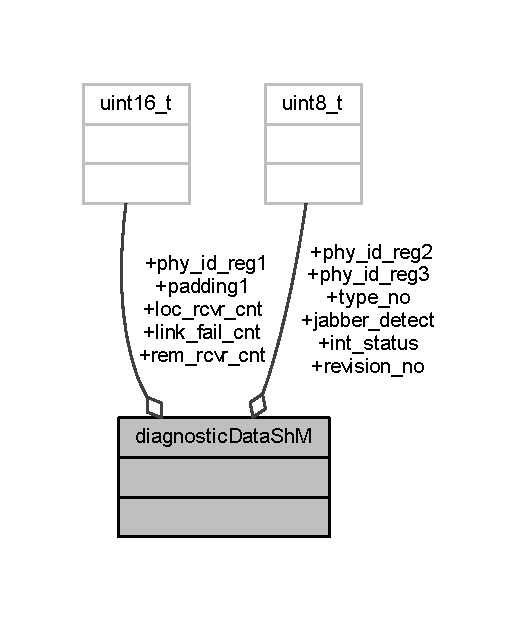
\includegraphics[width=257pt]{structdiagnostic_data_sh_m__coll__graph}
\end{center}
\end{figure}
\subsection*{Public Attributes}
\begin{DoxyCompactItemize}
\item 
uint8\+\_\+t \mbox{\hyperlink{structdiagnostic_data_sh_m_ac2b66edcfd19f4d451164ac0db6311ba}{jabber\+\_\+detect}}
\item 
uint16\+\_\+t \mbox{\hyperlink{structdiagnostic_data_sh_m_a5412678306937d33f7ce540392dd3bee}{phy\+\_\+id\+\_\+reg1}}
\item 
uint8\+\_\+t \mbox{\hyperlink{structdiagnostic_data_sh_m_abb2c872d63a3cba2131ec247be6fd488}{phy\+\_\+id\+\_\+reg2}}
\item 
uint8\+\_\+t \mbox{\hyperlink{structdiagnostic_data_sh_m_abaf7cabbe086caa5a4633769892634b8}{type\+\_\+no}}
\item 
uint8\+\_\+t \mbox{\hyperlink{structdiagnostic_data_sh_m_ab92c40adccff7a9ed25309f1ff536a31}{revision\+\_\+no}}
\item 
uint8\+\_\+t \mbox{\hyperlink{structdiagnostic_data_sh_m_ac3d2a208220c5b1783c611c335991838}{phy\+\_\+id\+\_\+reg3}}
\item 
uint8\+\_\+t \mbox{\hyperlink{structdiagnostic_data_sh_m_ab2ca00889c6139adfe8fa5b64cf6936d}{int\+\_\+status}}
\item 
uint16\+\_\+t \mbox{\hyperlink{structdiagnostic_data_sh_m_ac2b66edcfd19f4d451164ac0db6311ba}{jabber\+\_\+detect}}
\item 
uint16\+\_\+t \mbox{\hyperlink{structdiagnostic_data_sh_m_abb2c872d63a3cba2131ec247be6fd488}{phy\+\_\+id\+\_\+reg2}}
\item 
uint16\+\_\+t \mbox{\hyperlink{structdiagnostic_data_sh_m_abaf7cabbe086caa5a4633769892634b8}{type\+\_\+no}}
\item 
uint16\+\_\+t \mbox{\hyperlink{structdiagnostic_data_sh_m_ab92c40adccff7a9ed25309f1ff536a31}{revision\+\_\+no}}
\item 
uint16\+\_\+t \mbox{\hyperlink{structdiagnostic_data_sh_m_ac3d2a208220c5b1783c611c335991838}{phy\+\_\+id\+\_\+reg3}}
\item 
uint16\+\_\+t \mbox{\hyperlink{structdiagnostic_data_sh_m_ab2ca00889c6139adfe8fa5b64cf6936d}{int\+\_\+status}}
\item 
uint16\+\_\+t \mbox{\hyperlink{structdiagnostic_data_sh_m_ac0c9f1dc4e8f935100b4c9840a873f36}{loc\+\_\+rcvr\+\_\+cnt}}
\item 
uint16\+\_\+t \mbox{\hyperlink{structdiagnostic_data_sh_m_a3f0bf956d0452b349d1d51dcc67e8600}{rem\+\_\+rcvr\+\_\+cnt}}
\item 
uint16\+\_\+t \mbox{\hyperlink{structdiagnostic_data_sh_m_a0d3efa05bf7a22241d54e6e6e9fb3732}{link\+\_\+fail\+\_\+cnt}}
\end{DoxyCompactItemize}


\subsection{Member Data Documentation}
\mbox{\Hypertarget{structdiagnostic_data_sh_m_ab2ca00889c6139adfe8fa5b64cf6936d}\label{structdiagnostic_data_sh_m_ab2ca00889c6139adfe8fa5b64cf6936d}} 
\index{diagnostic\+Data\+ShM@{diagnostic\+Data\+ShM}!int\+\_\+status@{int\+\_\+status}}
\index{int\+\_\+status@{int\+\_\+status}!diagnostic\+Data\+ShM@{diagnostic\+Data\+ShM}}
\subsubsection{\texorpdfstring{int\+\_\+status}{int\_status}\hspace{0.1cm}{\footnotesize\ttfamily [1/2]}}
{\footnotesize\ttfamily uint16\+\_\+t diagnostic\+Data\+Sh\+M\+::int\+\_\+status}

\mbox{\Hypertarget{structdiagnostic_data_sh_m_ab2ca00889c6139adfe8fa5b64cf6936d}\label{structdiagnostic_data_sh_m_ab2ca00889c6139adfe8fa5b64cf6936d}} 
\index{diagnostic\+Data\+ShM@{diagnostic\+Data\+ShM}!int\+\_\+status@{int\+\_\+status}}
\index{int\+\_\+status@{int\+\_\+status}!diagnostic\+Data\+ShM@{diagnostic\+Data\+ShM}}
\subsubsection{\texorpdfstring{int\+\_\+status}{int\_status}\hspace{0.1cm}{\footnotesize\ttfamily [2/2]}}
{\footnotesize\ttfamily uint16\+\_\+t diagnostic\+Data\+Sh\+M\+::int\+\_\+status}

\mbox{\Hypertarget{structdiagnostic_data_sh_m_ac2b66edcfd19f4d451164ac0db6311ba}\label{structdiagnostic_data_sh_m_ac2b66edcfd19f4d451164ac0db6311ba}} 
\index{diagnostic\+Data\+ShM@{diagnostic\+Data\+ShM}!jabber\+\_\+detect@{jabber\+\_\+detect}}
\index{jabber\+\_\+detect@{jabber\+\_\+detect}!diagnostic\+Data\+ShM@{diagnostic\+Data\+ShM}}
\subsubsection{\texorpdfstring{jabber\+\_\+detect}{jabber\_detect}\hspace{0.1cm}{\footnotesize\ttfamily [1/2]}}
{\footnotesize\ttfamily uint16\+\_\+t diagnostic\+Data\+Sh\+M\+::jabber\+\_\+detect}

\mbox{\Hypertarget{structdiagnostic_data_sh_m_ac2b66edcfd19f4d451164ac0db6311ba}\label{structdiagnostic_data_sh_m_ac2b66edcfd19f4d451164ac0db6311ba}} 
\index{diagnostic\+Data\+ShM@{diagnostic\+Data\+ShM}!jabber\+\_\+detect@{jabber\+\_\+detect}}
\index{jabber\+\_\+detect@{jabber\+\_\+detect}!diagnostic\+Data\+ShM@{diagnostic\+Data\+ShM}}
\subsubsection{\texorpdfstring{jabber\+\_\+detect}{jabber\_detect}\hspace{0.1cm}{\footnotesize\ttfamily [2/2]}}
{\footnotesize\ttfamily uint16\+\_\+t diagnostic\+Data\+Sh\+M\+::jabber\+\_\+detect}

\mbox{\Hypertarget{structdiagnostic_data_sh_m_a0d3efa05bf7a22241d54e6e6e9fb3732}\label{structdiagnostic_data_sh_m_a0d3efa05bf7a22241d54e6e6e9fb3732}} 
\index{diagnostic\+Data\+ShM@{diagnostic\+Data\+ShM}!link\+\_\+fail\+\_\+cnt@{link\+\_\+fail\+\_\+cnt}}
\index{link\+\_\+fail\+\_\+cnt@{link\+\_\+fail\+\_\+cnt}!diagnostic\+Data\+ShM@{diagnostic\+Data\+ShM}}
\subsubsection{\texorpdfstring{link\+\_\+fail\+\_\+cnt}{link\_fail\_cnt}}
{\footnotesize\ttfamily uint16\+\_\+t diagnostic\+Data\+Sh\+M\+::link\+\_\+fail\+\_\+cnt}

\mbox{\Hypertarget{structdiagnostic_data_sh_m_ac0c9f1dc4e8f935100b4c9840a873f36}\label{structdiagnostic_data_sh_m_ac0c9f1dc4e8f935100b4c9840a873f36}} 
\index{diagnostic\+Data\+ShM@{diagnostic\+Data\+ShM}!loc\+\_\+rcvr\+\_\+cnt@{loc\+\_\+rcvr\+\_\+cnt}}
\index{loc\+\_\+rcvr\+\_\+cnt@{loc\+\_\+rcvr\+\_\+cnt}!diagnostic\+Data\+ShM@{diagnostic\+Data\+ShM}}
\subsubsection{\texorpdfstring{loc\+\_\+rcvr\+\_\+cnt}{loc\_rcvr\_cnt}}
{\footnotesize\ttfamily uint16\+\_\+t diagnostic\+Data\+Sh\+M\+::loc\+\_\+rcvr\+\_\+cnt}

\mbox{\Hypertarget{structdiagnostic_data_sh_m_a5412678306937d33f7ce540392dd3bee}\label{structdiagnostic_data_sh_m_a5412678306937d33f7ce540392dd3bee}} 
\index{diagnostic\+Data\+ShM@{diagnostic\+Data\+ShM}!phy\+\_\+id\+\_\+reg1@{phy\+\_\+id\+\_\+reg1}}
\index{phy\+\_\+id\+\_\+reg1@{phy\+\_\+id\+\_\+reg1}!diagnostic\+Data\+ShM@{diagnostic\+Data\+ShM}}
\subsubsection{\texorpdfstring{phy\+\_\+id\+\_\+reg1}{phy\_id\_reg1}}
{\footnotesize\ttfamily uint16\+\_\+t diagnostic\+Data\+Sh\+M\+::phy\+\_\+id\+\_\+reg1}

\mbox{\Hypertarget{structdiagnostic_data_sh_m_abb2c872d63a3cba2131ec247be6fd488}\label{structdiagnostic_data_sh_m_abb2c872d63a3cba2131ec247be6fd488}} 
\index{diagnostic\+Data\+ShM@{diagnostic\+Data\+ShM}!phy\+\_\+id\+\_\+reg2@{phy\+\_\+id\+\_\+reg2}}
\index{phy\+\_\+id\+\_\+reg2@{phy\+\_\+id\+\_\+reg2}!diagnostic\+Data\+ShM@{diagnostic\+Data\+ShM}}
\subsubsection{\texorpdfstring{phy\+\_\+id\+\_\+reg2}{phy\_id\_reg2}\hspace{0.1cm}{\footnotesize\ttfamily [1/2]}}
{\footnotesize\ttfamily uint16\+\_\+t diagnostic\+Data\+Sh\+M\+::phy\+\_\+id\+\_\+reg2}

\mbox{\Hypertarget{structdiagnostic_data_sh_m_abb2c872d63a3cba2131ec247be6fd488}\label{structdiagnostic_data_sh_m_abb2c872d63a3cba2131ec247be6fd488}} 
\index{diagnostic\+Data\+ShM@{diagnostic\+Data\+ShM}!phy\+\_\+id\+\_\+reg2@{phy\+\_\+id\+\_\+reg2}}
\index{phy\+\_\+id\+\_\+reg2@{phy\+\_\+id\+\_\+reg2}!diagnostic\+Data\+ShM@{diagnostic\+Data\+ShM}}
\subsubsection{\texorpdfstring{phy\+\_\+id\+\_\+reg2}{phy\_id\_reg2}\hspace{0.1cm}{\footnotesize\ttfamily [2/2]}}
{\footnotesize\ttfamily uint16\+\_\+t diagnostic\+Data\+Sh\+M\+::phy\+\_\+id\+\_\+reg2}

\mbox{\Hypertarget{structdiagnostic_data_sh_m_ac3d2a208220c5b1783c611c335991838}\label{structdiagnostic_data_sh_m_ac3d2a208220c5b1783c611c335991838}} 
\index{diagnostic\+Data\+ShM@{diagnostic\+Data\+ShM}!phy\+\_\+id\+\_\+reg3@{phy\+\_\+id\+\_\+reg3}}
\index{phy\+\_\+id\+\_\+reg3@{phy\+\_\+id\+\_\+reg3}!diagnostic\+Data\+ShM@{diagnostic\+Data\+ShM}}
\subsubsection{\texorpdfstring{phy\+\_\+id\+\_\+reg3}{phy\_id\_reg3}\hspace{0.1cm}{\footnotesize\ttfamily [1/2]}}
{\footnotesize\ttfamily uint16\+\_\+t diagnostic\+Data\+Sh\+M\+::phy\+\_\+id\+\_\+reg3}

\mbox{\Hypertarget{structdiagnostic_data_sh_m_ac3d2a208220c5b1783c611c335991838}\label{structdiagnostic_data_sh_m_ac3d2a208220c5b1783c611c335991838}} 
\index{diagnostic\+Data\+ShM@{diagnostic\+Data\+ShM}!phy\+\_\+id\+\_\+reg3@{phy\+\_\+id\+\_\+reg3}}
\index{phy\+\_\+id\+\_\+reg3@{phy\+\_\+id\+\_\+reg3}!diagnostic\+Data\+ShM@{diagnostic\+Data\+ShM}}
\subsubsection{\texorpdfstring{phy\+\_\+id\+\_\+reg3}{phy\_id\_reg3}\hspace{0.1cm}{\footnotesize\ttfamily [2/2]}}
{\footnotesize\ttfamily uint16\+\_\+t diagnostic\+Data\+Sh\+M\+::phy\+\_\+id\+\_\+reg3}

\mbox{\Hypertarget{structdiagnostic_data_sh_m_a3f0bf956d0452b349d1d51dcc67e8600}\label{structdiagnostic_data_sh_m_a3f0bf956d0452b349d1d51dcc67e8600}} 
\index{diagnostic\+Data\+ShM@{diagnostic\+Data\+ShM}!rem\+\_\+rcvr\+\_\+cnt@{rem\+\_\+rcvr\+\_\+cnt}}
\index{rem\+\_\+rcvr\+\_\+cnt@{rem\+\_\+rcvr\+\_\+cnt}!diagnostic\+Data\+ShM@{diagnostic\+Data\+ShM}}
\subsubsection{\texorpdfstring{rem\+\_\+rcvr\+\_\+cnt}{rem\_rcvr\_cnt}}
{\footnotesize\ttfamily uint16\+\_\+t diagnostic\+Data\+Sh\+M\+::rem\+\_\+rcvr\+\_\+cnt}

\mbox{\Hypertarget{structdiagnostic_data_sh_m_ab92c40adccff7a9ed25309f1ff536a31}\label{structdiagnostic_data_sh_m_ab92c40adccff7a9ed25309f1ff536a31}} 
\index{diagnostic\+Data\+ShM@{diagnostic\+Data\+ShM}!revision\+\_\+no@{revision\+\_\+no}}
\index{revision\+\_\+no@{revision\+\_\+no}!diagnostic\+Data\+ShM@{diagnostic\+Data\+ShM}}
\subsubsection{\texorpdfstring{revision\+\_\+no}{revision\_no}\hspace{0.1cm}{\footnotesize\ttfamily [1/2]}}
{\footnotesize\ttfamily uint16\+\_\+t diagnostic\+Data\+Sh\+M\+::revision\+\_\+no}

\mbox{\Hypertarget{structdiagnostic_data_sh_m_ab92c40adccff7a9ed25309f1ff536a31}\label{structdiagnostic_data_sh_m_ab92c40adccff7a9ed25309f1ff536a31}} 
\index{diagnostic\+Data\+ShM@{diagnostic\+Data\+ShM}!revision\+\_\+no@{revision\+\_\+no}}
\index{revision\+\_\+no@{revision\+\_\+no}!diagnostic\+Data\+ShM@{diagnostic\+Data\+ShM}}
\subsubsection{\texorpdfstring{revision\+\_\+no}{revision\_no}\hspace{0.1cm}{\footnotesize\ttfamily [2/2]}}
{\footnotesize\ttfamily uint16\+\_\+t diagnostic\+Data\+Sh\+M\+::revision\+\_\+no}

\mbox{\Hypertarget{structdiagnostic_data_sh_m_abaf7cabbe086caa5a4633769892634b8}\label{structdiagnostic_data_sh_m_abaf7cabbe086caa5a4633769892634b8}} 
\index{diagnostic\+Data\+ShM@{diagnostic\+Data\+ShM}!type\+\_\+no@{type\+\_\+no}}
\index{type\+\_\+no@{type\+\_\+no}!diagnostic\+Data\+ShM@{diagnostic\+Data\+ShM}}
\subsubsection{\texorpdfstring{type\+\_\+no}{type\_no}\hspace{0.1cm}{\footnotesize\ttfamily [1/2]}}
{\footnotesize\ttfamily uint16\+\_\+t diagnostic\+Data\+Sh\+M\+::type\+\_\+no}

\mbox{\Hypertarget{structdiagnostic_data_sh_m_abaf7cabbe086caa5a4633769892634b8}\label{structdiagnostic_data_sh_m_abaf7cabbe086caa5a4633769892634b8}} 
\index{diagnostic\+Data\+ShM@{diagnostic\+Data\+ShM}!type\+\_\+no@{type\+\_\+no}}
\index{type\+\_\+no@{type\+\_\+no}!diagnostic\+Data\+ShM@{diagnostic\+Data\+ShM}}
\subsubsection{\texorpdfstring{type\+\_\+no}{type\_no}\hspace{0.1cm}{\footnotesize\ttfamily [2/2]}}
{\footnotesize\ttfamily uint16\+\_\+t diagnostic\+Data\+Sh\+M\+::type\+\_\+no}



The documentation for this struct was generated from the following files\+:\begin{DoxyCompactItemize}
\item 
\mbox{\hyperlink{__module3_8h}{\+\_\+module3.\+h}}\item 
\mbox{\hyperlink{module3_8h}{module3.\+h}}\item 
\mbox{\hyperlink{module_one_read_eth_phy_8h}{module\+One\+Read\+Eth\+Phy.\+h}}\item 
\mbox{\hyperlink{module_two_communication_8h}{module\+Two\+Communication.\+h}}\end{DoxyCompactItemize}

\hypertarget{structerror_struct}{}\section{error\+Struct Struct Reference}
\label{structerror_struct}\index{error\+Struct@{error\+Struct}}


{\ttfamily \#include $<$module\+One\+Read\+Eth\+Phy.\+h$>$}



Collaboration diagram for error\+Struct\+:
\nopagebreak
\begin{figure}[H]
\begin{center}
\leavevmode
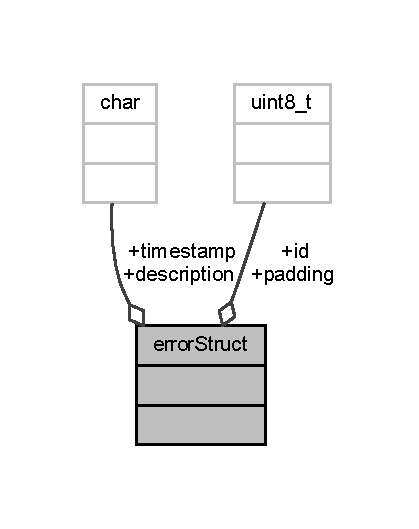
\includegraphics[width=201pt]{structerror_struct__coll__graph}
\end{center}
\end{figure}
\subsection*{Public Attributes}
\begin{DoxyCompactItemize}
\item 
char \mbox{\hyperlink{structerror_struct_a51e5ae4be96680737622f257e2eb2479}{timestamp}} \mbox{[}26\mbox{]}
\item 
uint8\+\_\+t \mbox{\hyperlink{structerror_struct_af07d527b0695dad43376f6658ca6d9d3}{id}}
\item 
char \mbox{\hyperlink{structerror_struct_aed437236613db32b2b56361e2cbf3ce6}{description}} \mbox{[}50\mbox{]}
\item 
uint8\+\_\+t \mbox{\hyperlink{structerror_struct_a14bf4c23e01145e362768dfdc4466737}{padding}}
\end{DoxyCompactItemize}


\subsection{Member Data Documentation}
\mbox{\Hypertarget{structerror_struct_aed437236613db32b2b56361e2cbf3ce6}\label{structerror_struct_aed437236613db32b2b56361e2cbf3ce6}} 
\index{error\+Struct@{error\+Struct}!description@{description}}
\index{description@{description}!error\+Struct@{error\+Struct}}
\subsubsection{\texorpdfstring{description}{description}}
{\footnotesize\ttfamily char error\+Struct\+::description}

\mbox{\Hypertarget{structerror_struct_af07d527b0695dad43376f6658ca6d9d3}\label{structerror_struct_af07d527b0695dad43376f6658ca6d9d3}} 
\index{error\+Struct@{error\+Struct}!id@{id}}
\index{id@{id}!error\+Struct@{error\+Struct}}
\subsubsection{\texorpdfstring{id}{id}}
{\footnotesize\ttfamily uint8\+\_\+t error\+Struct\+::id}

\mbox{\Hypertarget{structerror_struct_a14bf4c23e01145e362768dfdc4466737}\label{structerror_struct_a14bf4c23e01145e362768dfdc4466737}} 
\index{error\+Struct@{error\+Struct}!padding@{padding}}
\index{padding@{padding}!error\+Struct@{error\+Struct}}
\subsubsection{\texorpdfstring{padding}{padding}}
{\footnotesize\ttfamily uint8\+\_\+t error\+Struct\+::padding}

\mbox{\Hypertarget{structerror_struct_a51e5ae4be96680737622f257e2eb2479}\label{structerror_struct_a51e5ae4be96680737622f257e2eb2479}} 
\index{error\+Struct@{error\+Struct}!timestamp@{timestamp}}
\index{timestamp@{timestamp}!error\+Struct@{error\+Struct}}
\subsubsection{\texorpdfstring{timestamp}{timestamp}}
{\footnotesize\ttfamily char error\+Struct\+::timestamp}



The documentation for this struct was generated from the following files\+:\begin{DoxyCompactItemize}
\item 
\mbox{\hyperlink{module_one_read_eth_phy_8h}{module\+One\+Read\+Eth\+Phy.\+h}}\item 
\mbox{\hyperlink{module_two_communication_8h}{module\+Two\+Communication.\+h}}\end{DoxyCompactItemize}

\hypertarget{class_main_window}{}\section{Main\+Window Class Reference}
\label{class_main_window}\index{Main\+Window@{Main\+Window}}


{\ttfamily \#include $<$mainwindow.\+h$>$}



Inheritance diagram for Main\+Window\+:
\nopagebreak
\begin{figure}[H]
\begin{center}
\leavevmode
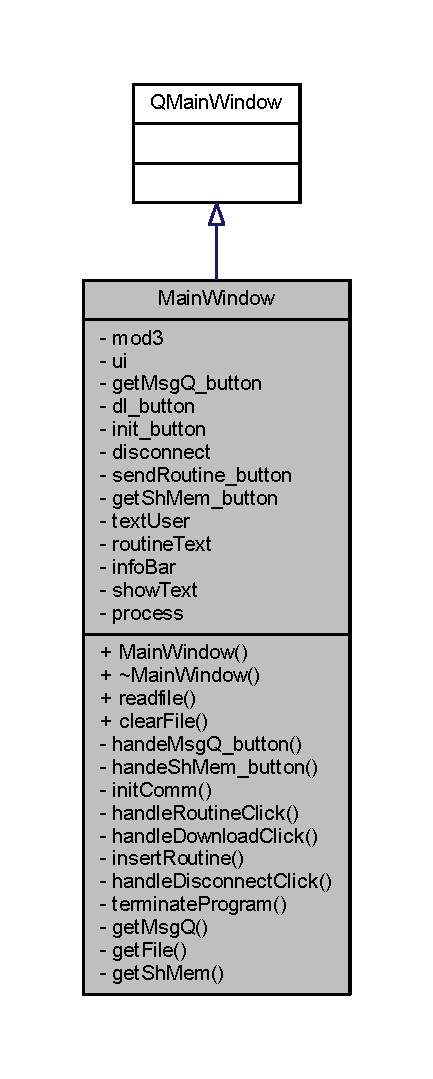
\includegraphics[width=208pt]{class_main_window__inherit__graph}
\end{center}
\end{figure}


Collaboration diagram for Main\+Window\+:
\nopagebreak
\begin{figure}[H]
\begin{center}
\leavevmode
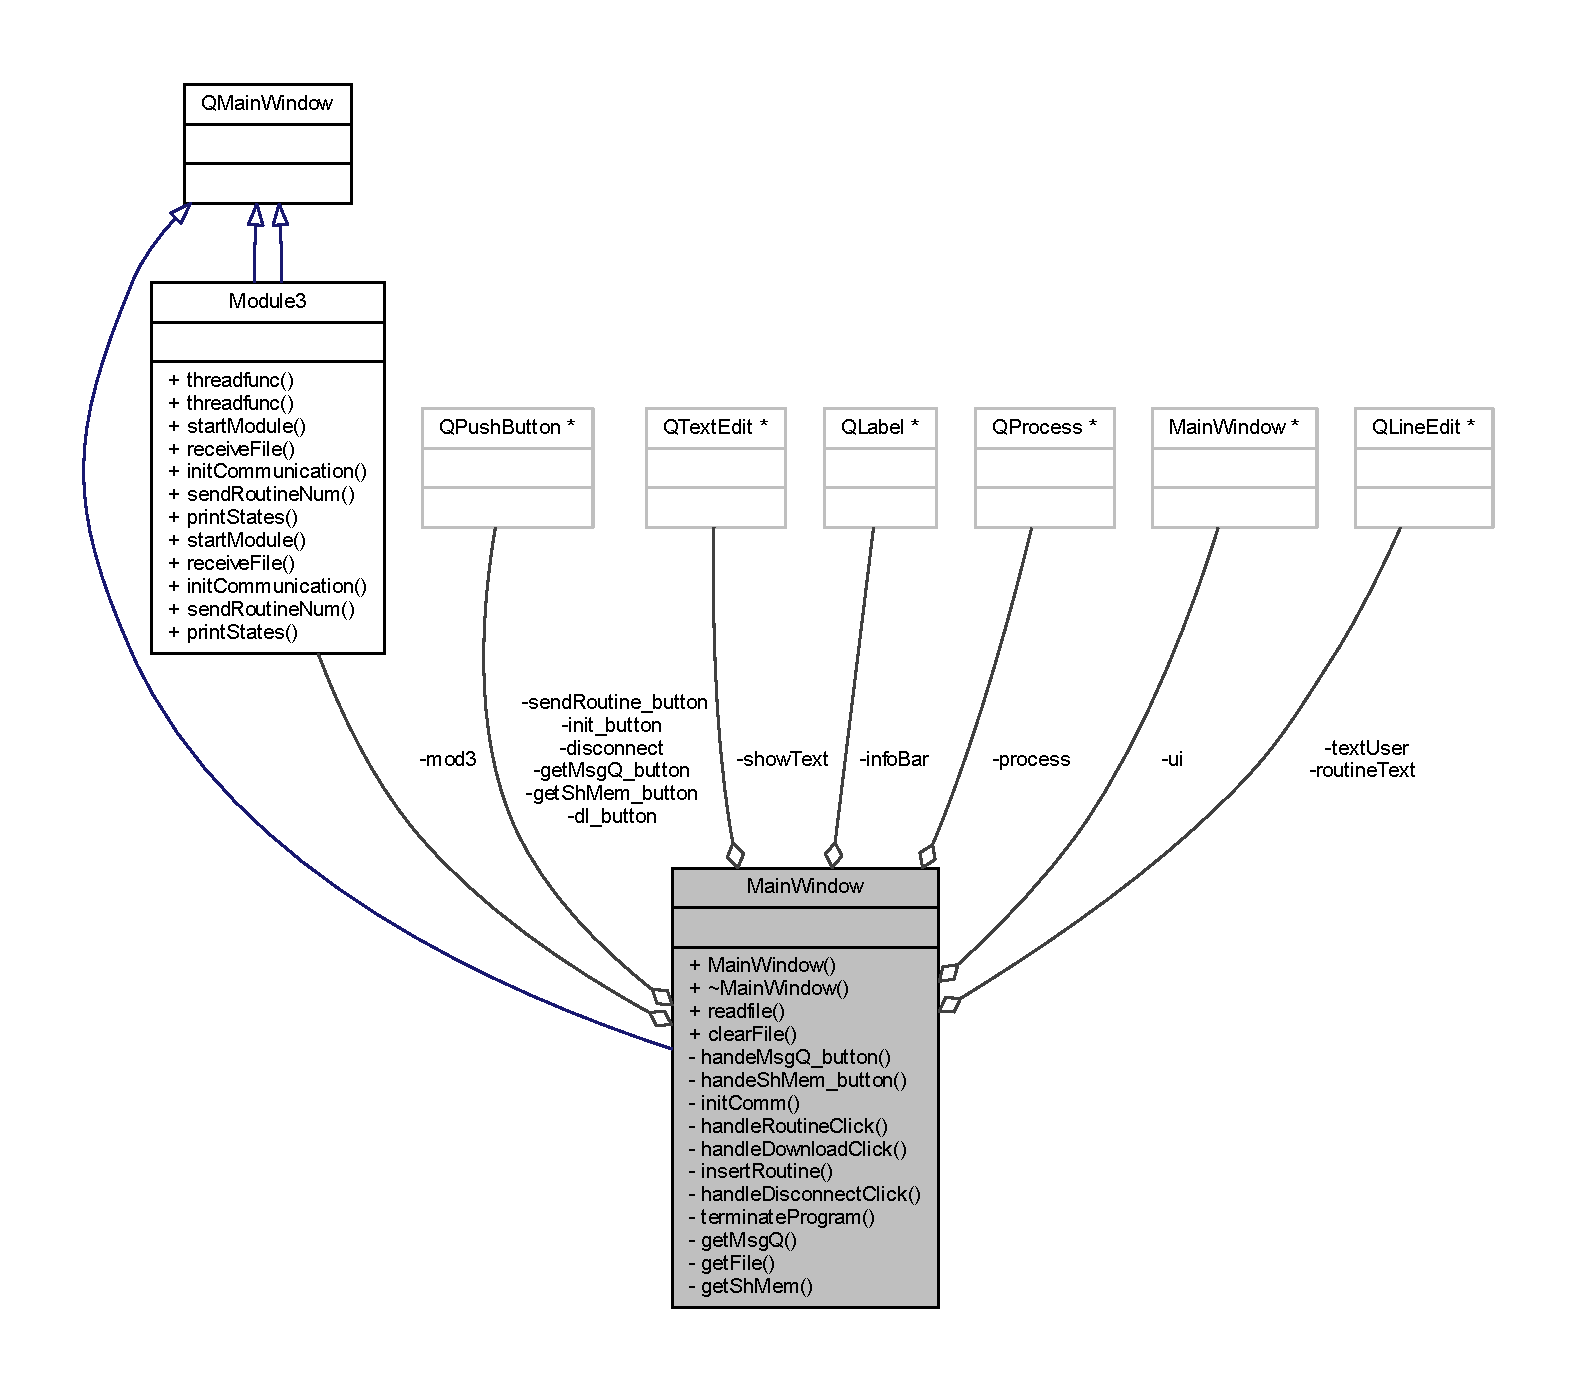
\includegraphics[width=350pt]{class_main_window__coll__graph}
\end{center}
\end{figure}
\subsection*{Signals}
\begin{DoxyCompactItemize}
\item 
void \mbox{\hyperlink{class_main_window_a0b1a3960102da5863d7d31570d2837b7}{get\+Msg\+Q\+Status}} ()
\item 
void \mbox{\hyperlink{class_main_window_af8f815f498b3ecec7c8e19dfbc8b6c47}{download\+File}} ()
\item 
void \mbox{\hyperlink{class_main_window_a491881163b44282206d1313243af5e2f}{get\+Sh\+Mem\+Status}} ()
\item 
void \mbox{\hyperlink{class_main_window_aadedb5af94649f8e8a16c6642aa7b319}{insert\+Routine\+Number}} ()
\item 
void \mbox{\hyperlink{class_main_window_a18ba5e9b20b321fec60894796e053ca5}{disconnect\+Clicked}} ()
\end{DoxyCompactItemize}
\subsection*{Public Member Functions}
\begin{DoxyCompactItemize}
\item 
\mbox{\hyperlink{class_main_window_a8b244be8b7b7db1b08de2a2acb9409db}{Main\+Window}} (Q\+Widget $\ast$parent=0)
\item 
\mbox{\hyperlink{class_main_window_ae98d00a93bc118200eeef9f9bba1dba7}{$\sim$\+Main\+Window}} ()
\item 
void \mbox{\hyperlink{class_main_window_a45eac78192a605f450c10b8c4b1bde81}{readfile}} ()
\item 
void \mbox{\hyperlink{class_main_window_abc60bc84ec0badc555d692af286f8053}{clear\+File}} ()
\end{DoxyCompactItemize}
\subsection*{Private Slots}
\begin{DoxyCompactItemize}
\item 
void \mbox{\hyperlink{class_main_window_a70df7ecf71e55431b4cdaee7c023b6b8}{hande\+Msg\+Q\+\_\+button}} ()
\item 
void \mbox{\hyperlink{class_main_window_a9edd35d94300c8e7ee118517848d2675}{hande\+Sh\+Mem\+\_\+button}} ()
\item 
void \mbox{\hyperlink{class_main_window_a3ae7677276119857e128f826c8b069c8}{init\+Comm}} ()
\item 
void \mbox{\hyperlink{class_main_window_abd7dc3af4e03fd257fcac427474ceeff}{handle\+Routine\+Click}} ()
\item 
void \mbox{\hyperlink{class_main_window_a19632dc3a31d674e845e237576bf8191}{handle\+Download\+Click}} ()
\item 
void \mbox{\hyperlink{class_main_window_a88b30e72fd13b54ddef7bf6e2bb08448}{insert\+Routine}} ()
\item 
void \mbox{\hyperlink{class_main_window_a9fab898ff6721d7811511a98e75150d6}{handle\+Disconnect\+Click}} ()
\item 
void \mbox{\hyperlink{class_main_window_aab2fed34f5ba1468a0c9ff35fcd79757}{terminate\+Program}} ()
\item 
void \mbox{\hyperlink{class_main_window_af0e609b7bacc38e1f25151a55b589222}{get\+MsgQ}} ()
\item 
void \mbox{\hyperlink{class_main_window_ae312fe1c0640df073ef40d7fbab3e1f9}{get\+File}} ()
\item 
void \mbox{\hyperlink{class_main_window_a707b068e9373c76cbb4d844b15d4b509}{get\+Sh\+Mem}} ()
\end{DoxyCompactItemize}
\subsection*{Private Attributes}
\begin{DoxyCompactItemize}
\item 
\mbox{\hyperlink{class_module3}{Module3}} \mbox{\hyperlink{class_main_window_a13d73f676f1bfdd6090677bbc17dc3bb}{mod3}}
\item 
Ui\+::\+Main\+Window $\ast$ \mbox{\hyperlink{class_main_window_a35466a70ed47252a0191168126a352a5}{ui}}
\item 
Q\+Push\+Button $\ast$ \mbox{\hyperlink{class_main_window_a33fff3efd2a06d6df2e37219d44d9d20}{get\+Msg\+Q\+\_\+button}}
\item 
Q\+Push\+Button $\ast$ \mbox{\hyperlink{class_main_window_afb9e7419ea1c7c1f109857ac8ed9e703}{dl\+\_\+button}}
\item 
Q\+Push\+Button $\ast$ \mbox{\hyperlink{class_main_window_ad1cf02a751bb3647114db947acebcaf5}{init\+\_\+button}}
\item 
Q\+Push\+Button $\ast$ \mbox{\hyperlink{class_main_window_a9d4a6f9ce2275a736abcedf0bba2bad9}{disconnect}}
\item 
Q\+Push\+Button $\ast$ \mbox{\hyperlink{class_main_window_a56a195b11e21a9e73cc7adad5b4666a1}{send\+Routine\+\_\+button}}
\item 
Q\+Push\+Button $\ast$ \mbox{\hyperlink{class_main_window_a26663544e9c5a627b73df4d060a9a06a}{get\+Sh\+Mem\+\_\+button}}
\item 
Q\+Line\+Edit $\ast$ \mbox{\hyperlink{class_main_window_a98c79855a722db4582f2c1f41b0369df}{text\+User}}
\item 
Q\+Line\+Edit $\ast$ \mbox{\hyperlink{class_main_window_ab016004d1d7ba0084b7201072c2ff193}{routine\+Text}}
\item 
Q\+Label $\ast$ \mbox{\hyperlink{class_main_window_ad1f2bbeefb0b2f010eef8fcd2f0b825f}{info\+Bar}}
\item 
Q\+Text\+Edit $\ast$ \mbox{\hyperlink{class_main_window_ae1fe4774da9daef3570ef190df36773e}{show\+Text}}
\item 
Q\+Process $\ast$ \mbox{\hyperlink{class_main_window_a9f6d60a6052813c8d83a0a2b3e1c9b2a}{process}}
\end{DoxyCompactItemize}


\subsection{Constructor \& Destructor Documentation}
\mbox{\Hypertarget{class_main_window_a8b244be8b7b7db1b08de2a2acb9409db}\label{class_main_window_a8b244be8b7b7db1b08de2a2acb9409db}} 
\index{Main\+Window@{Main\+Window}!Main\+Window@{Main\+Window}}
\index{Main\+Window@{Main\+Window}!Main\+Window@{Main\+Window}}
\subsubsection{\texorpdfstring{Main\+Window()}{MainWindow()}}
{\footnotesize\ttfamily Main\+Window\+::\+Main\+Window (\begin{DoxyParamCaption}\item[{Q\+Widget $\ast$}]{parent = {\ttfamily 0} }\end{DoxyParamCaption})\hspace{0.3cm}{\ttfamily [explicit]}}

Here is the call graph for this function\+:
\nopagebreak
\begin{figure}[H]
\begin{center}
\leavevmode
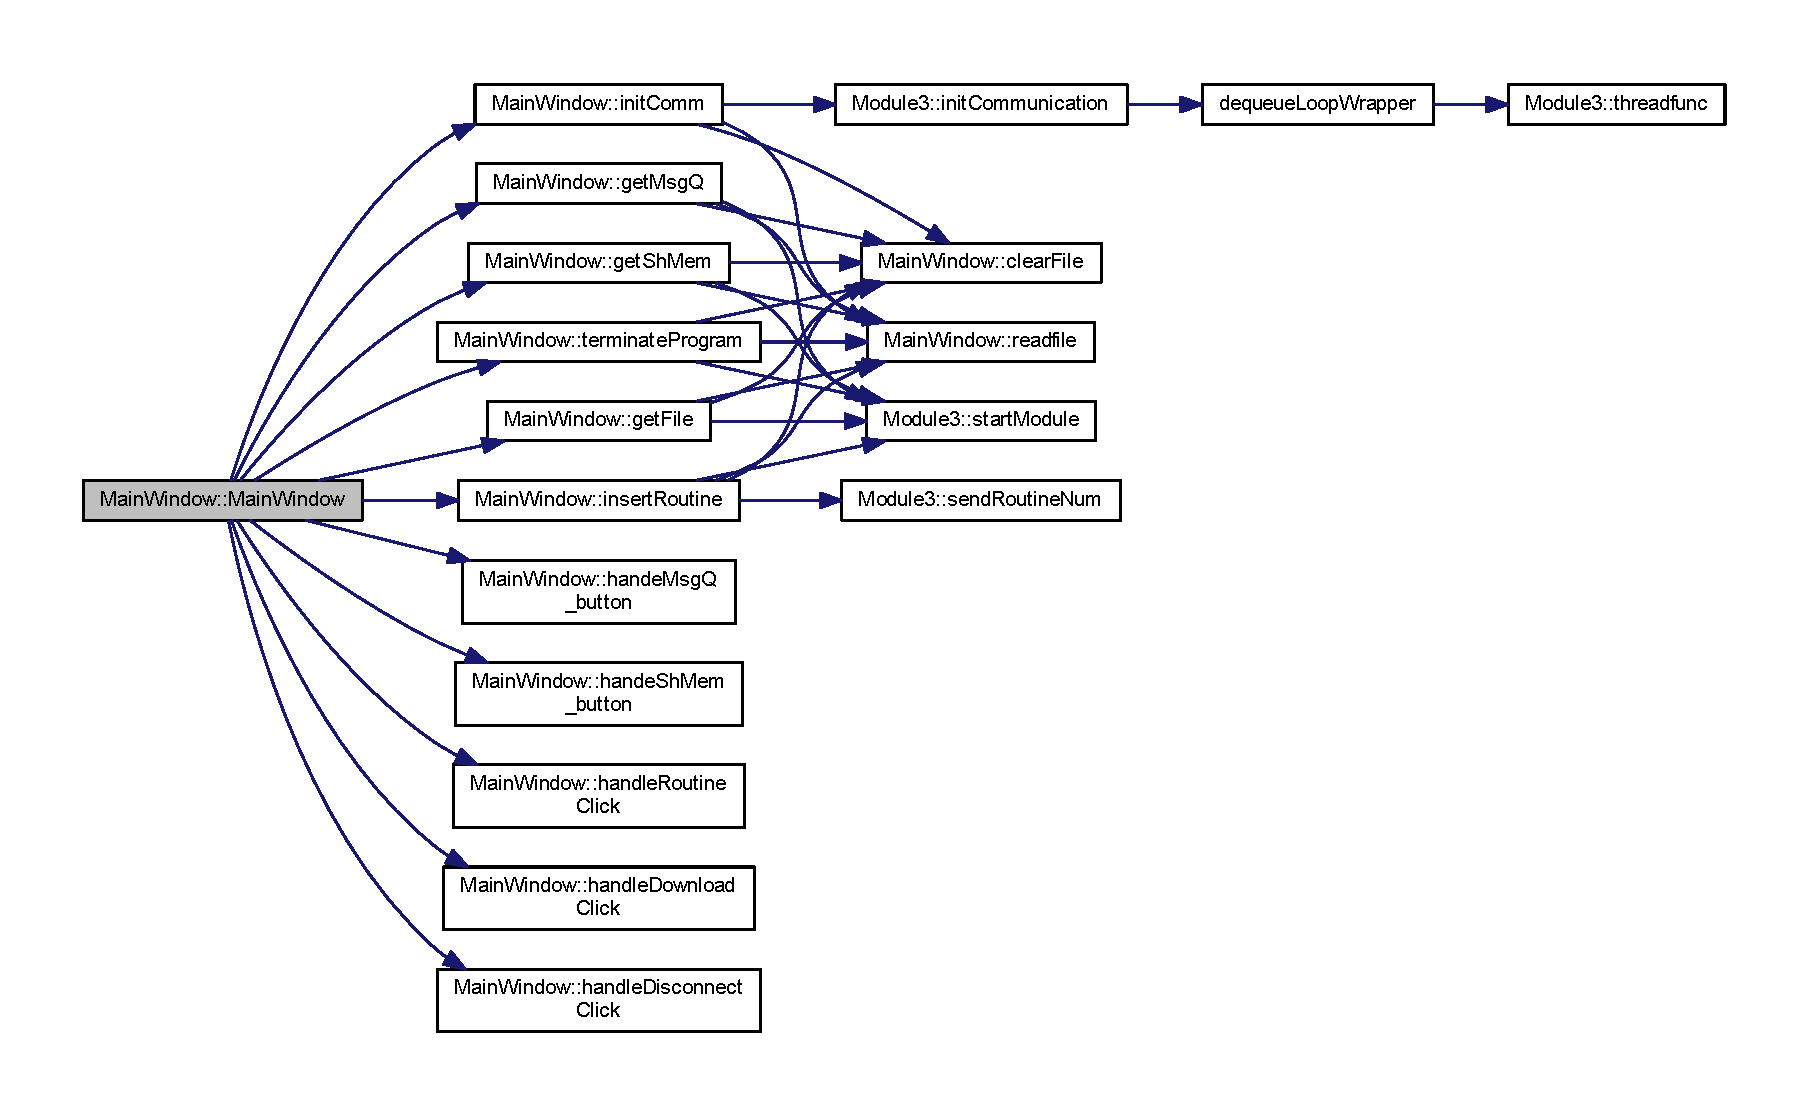
\includegraphics[width=350pt]{class_main_window_a8b244be8b7b7db1b08de2a2acb9409db_cgraph}
\end{center}
\end{figure}
\mbox{\Hypertarget{class_main_window_ae98d00a93bc118200eeef9f9bba1dba7}\label{class_main_window_ae98d00a93bc118200eeef9f9bba1dba7}} 
\index{Main\+Window@{Main\+Window}!````~Main\+Window@{$\sim$\+Main\+Window}}
\index{````~Main\+Window@{$\sim$\+Main\+Window}!Main\+Window@{Main\+Window}}
\subsubsection{\texorpdfstring{$\sim$\+Main\+Window()}{~MainWindow()}}
{\footnotesize\ttfamily Main\+Window\+::$\sim$\+Main\+Window (\begin{DoxyParamCaption}{ }\end{DoxyParamCaption})}



\subsection{Member Function Documentation}
\mbox{\Hypertarget{class_main_window_abc60bc84ec0badc555d692af286f8053}\label{class_main_window_abc60bc84ec0badc555d692af286f8053}} 
\index{Main\+Window@{Main\+Window}!clear\+File@{clear\+File}}
\index{clear\+File@{clear\+File}!Main\+Window@{Main\+Window}}
\subsubsection{\texorpdfstring{clear\+File()}{clearFile()}}
{\footnotesize\ttfamily void Main\+Window\+::clear\+File (\begin{DoxyParamCaption}{ }\end{DoxyParamCaption})}

\mbox{\Hypertarget{class_main_window_a18ba5e9b20b321fec60894796e053ca5}\label{class_main_window_a18ba5e9b20b321fec60894796e053ca5}} 
\index{Main\+Window@{Main\+Window}!disconnect\+Clicked@{disconnect\+Clicked}}
\index{disconnect\+Clicked@{disconnect\+Clicked}!Main\+Window@{Main\+Window}}
\subsubsection{\texorpdfstring{disconnect\+Clicked}{disconnectClicked}}
{\footnotesize\ttfamily void Main\+Window\+::disconnect\+Clicked (\begin{DoxyParamCaption}{ }\end{DoxyParamCaption})\hspace{0.3cm}{\ttfamily [signal]}}

\mbox{\Hypertarget{class_main_window_af8f815f498b3ecec7c8e19dfbc8b6c47}\label{class_main_window_af8f815f498b3ecec7c8e19dfbc8b6c47}} 
\index{Main\+Window@{Main\+Window}!download\+File@{download\+File}}
\index{download\+File@{download\+File}!Main\+Window@{Main\+Window}}
\subsubsection{\texorpdfstring{download\+File}{downloadFile}}
{\footnotesize\ttfamily void Main\+Window\+::download\+File (\begin{DoxyParamCaption}{ }\end{DoxyParamCaption})\hspace{0.3cm}{\ttfamily [signal]}}

\mbox{\Hypertarget{class_main_window_ae312fe1c0640df073ef40d7fbab3e1f9}\label{class_main_window_ae312fe1c0640df073ef40d7fbab3e1f9}} 
\index{Main\+Window@{Main\+Window}!get\+File@{get\+File}}
\index{get\+File@{get\+File}!Main\+Window@{Main\+Window}}
\subsubsection{\texorpdfstring{get\+File}{getFile}}
{\footnotesize\ttfamily void Main\+Window\+::get\+File (\begin{DoxyParamCaption}{ }\end{DoxyParamCaption})\hspace{0.3cm}{\ttfamily [private]}, {\ttfamily [slot]}}

Here is the call graph for this function\+:
\nopagebreak
\begin{figure}[H]
\begin{center}
\leavevmode
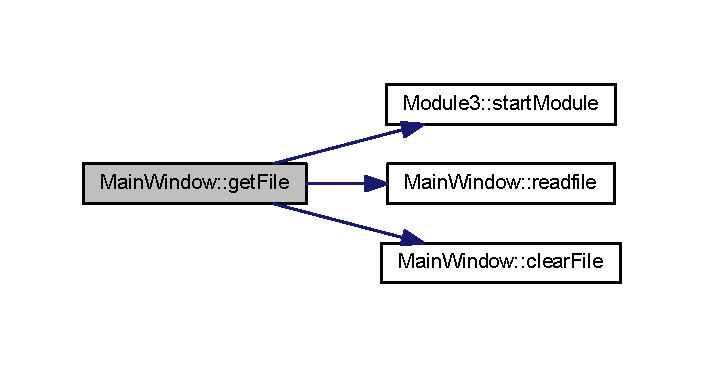
\includegraphics[width=338pt]{class_main_window_ae312fe1c0640df073ef40d7fbab3e1f9_cgraph}
\end{center}
\end{figure}
\mbox{\Hypertarget{class_main_window_af0e609b7bacc38e1f25151a55b589222}\label{class_main_window_af0e609b7bacc38e1f25151a55b589222}} 
\index{Main\+Window@{Main\+Window}!get\+MsgQ@{get\+MsgQ}}
\index{get\+MsgQ@{get\+MsgQ}!Main\+Window@{Main\+Window}}
\subsubsection{\texorpdfstring{get\+MsgQ}{getMsgQ}}
{\footnotesize\ttfamily void Main\+Window\+::get\+MsgQ (\begin{DoxyParamCaption}{ }\end{DoxyParamCaption})\hspace{0.3cm}{\ttfamily [private]}, {\ttfamily [slot]}}

Here is the call graph for this function\+:
\nopagebreak
\begin{figure}[H]
\begin{center}
\leavevmode
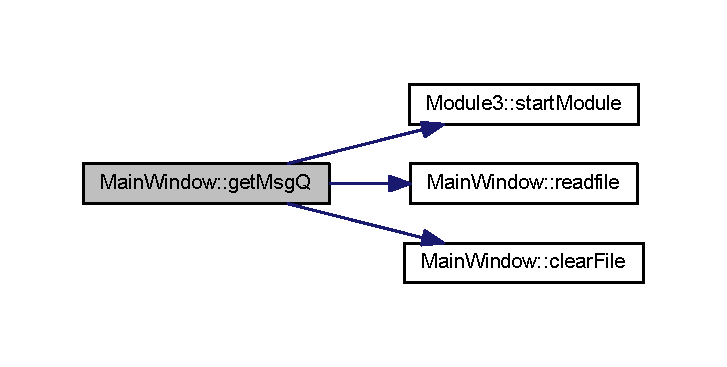
\includegraphics[width=349pt]{class_main_window_af0e609b7bacc38e1f25151a55b589222_cgraph}
\end{center}
\end{figure}
\mbox{\Hypertarget{class_main_window_a0b1a3960102da5863d7d31570d2837b7}\label{class_main_window_a0b1a3960102da5863d7d31570d2837b7}} 
\index{Main\+Window@{Main\+Window}!get\+Msg\+Q\+Status@{get\+Msg\+Q\+Status}}
\index{get\+Msg\+Q\+Status@{get\+Msg\+Q\+Status}!Main\+Window@{Main\+Window}}
\subsubsection{\texorpdfstring{get\+Msg\+Q\+Status}{getMsgQStatus}}
{\footnotesize\ttfamily void Main\+Window\+::get\+Msg\+Q\+Status (\begin{DoxyParamCaption}{ }\end{DoxyParamCaption})\hspace{0.3cm}{\ttfamily [signal]}}

\mbox{\Hypertarget{class_main_window_a707b068e9373c76cbb4d844b15d4b509}\label{class_main_window_a707b068e9373c76cbb4d844b15d4b509}} 
\index{Main\+Window@{Main\+Window}!get\+Sh\+Mem@{get\+Sh\+Mem}}
\index{get\+Sh\+Mem@{get\+Sh\+Mem}!Main\+Window@{Main\+Window}}
\subsubsection{\texorpdfstring{get\+Sh\+Mem}{getShMem}}
{\footnotesize\ttfamily void Main\+Window\+::get\+Sh\+Mem (\begin{DoxyParamCaption}{ }\end{DoxyParamCaption})\hspace{0.3cm}{\ttfamily [private]}, {\ttfamily [slot]}}

Here is the call graph for this function\+:
\nopagebreak
\begin{figure}[H]
\begin{center}
\leavevmode
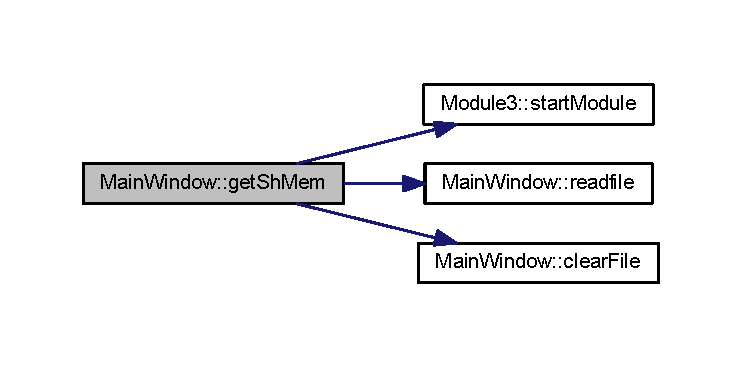
\includegraphics[width=350pt]{class_main_window_a707b068e9373c76cbb4d844b15d4b509_cgraph}
\end{center}
\end{figure}
\mbox{\Hypertarget{class_main_window_a491881163b44282206d1313243af5e2f}\label{class_main_window_a491881163b44282206d1313243af5e2f}} 
\index{Main\+Window@{Main\+Window}!get\+Sh\+Mem\+Status@{get\+Sh\+Mem\+Status}}
\index{get\+Sh\+Mem\+Status@{get\+Sh\+Mem\+Status}!Main\+Window@{Main\+Window}}
\subsubsection{\texorpdfstring{get\+Sh\+Mem\+Status}{getShMemStatus}}
{\footnotesize\ttfamily void Main\+Window\+::get\+Sh\+Mem\+Status (\begin{DoxyParamCaption}{ }\end{DoxyParamCaption})\hspace{0.3cm}{\ttfamily [signal]}}

\mbox{\Hypertarget{class_main_window_a70df7ecf71e55431b4cdaee7c023b6b8}\label{class_main_window_a70df7ecf71e55431b4cdaee7c023b6b8}} 
\index{Main\+Window@{Main\+Window}!hande\+Msg\+Q\+\_\+button@{hande\+Msg\+Q\+\_\+button}}
\index{hande\+Msg\+Q\+\_\+button@{hande\+Msg\+Q\+\_\+button}!Main\+Window@{Main\+Window}}
\subsubsection{\texorpdfstring{hande\+Msg\+Q\+\_\+button}{handeMsgQ\_button}}
{\footnotesize\ttfamily void Main\+Window\+::hande\+Msg\+Q\+\_\+button (\begin{DoxyParamCaption}{ }\end{DoxyParamCaption})\hspace{0.3cm}{\ttfamily [private]}, {\ttfamily [slot]}}

\mbox{\Hypertarget{class_main_window_a9edd35d94300c8e7ee118517848d2675}\label{class_main_window_a9edd35d94300c8e7ee118517848d2675}} 
\index{Main\+Window@{Main\+Window}!hande\+Sh\+Mem\+\_\+button@{hande\+Sh\+Mem\+\_\+button}}
\index{hande\+Sh\+Mem\+\_\+button@{hande\+Sh\+Mem\+\_\+button}!Main\+Window@{Main\+Window}}
\subsubsection{\texorpdfstring{hande\+Sh\+Mem\+\_\+button}{handeShMem\_button}}
{\footnotesize\ttfamily void Main\+Window\+::hande\+Sh\+Mem\+\_\+button (\begin{DoxyParamCaption}{ }\end{DoxyParamCaption})\hspace{0.3cm}{\ttfamily [private]}, {\ttfamily [slot]}}

\mbox{\Hypertarget{class_main_window_a9fab898ff6721d7811511a98e75150d6}\label{class_main_window_a9fab898ff6721d7811511a98e75150d6}} 
\index{Main\+Window@{Main\+Window}!handle\+Disconnect\+Click@{handle\+Disconnect\+Click}}
\index{handle\+Disconnect\+Click@{handle\+Disconnect\+Click}!Main\+Window@{Main\+Window}}
\subsubsection{\texorpdfstring{handle\+Disconnect\+Click}{handleDisconnectClick}}
{\footnotesize\ttfamily void Main\+Window\+::handle\+Disconnect\+Click (\begin{DoxyParamCaption}{ }\end{DoxyParamCaption})\hspace{0.3cm}{\ttfamily [private]}, {\ttfamily [slot]}}

\mbox{\Hypertarget{class_main_window_a19632dc3a31d674e845e237576bf8191}\label{class_main_window_a19632dc3a31d674e845e237576bf8191}} 
\index{Main\+Window@{Main\+Window}!handle\+Download\+Click@{handle\+Download\+Click}}
\index{handle\+Download\+Click@{handle\+Download\+Click}!Main\+Window@{Main\+Window}}
\subsubsection{\texorpdfstring{handle\+Download\+Click}{handleDownloadClick}}
{\footnotesize\ttfamily void Main\+Window\+::handle\+Download\+Click (\begin{DoxyParamCaption}{ }\end{DoxyParamCaption})\hspace{0.3cm}{\ttfamily [private]}, {\ttfamily [slot]}}

\mbox{\Hypertarget{class_main_window_abd7dc3af4e03fd257fcac427474ceeff}\label{class_main_window_abd7dc3af4e03fd257fcac427474ceeff}} 
\index{Main\+Window@{Main\+Window}!handle\+Routine\+Click@{handle\+Routine\+Click}}
\index{handle\+Routine\+Click@{handle\+Routine\+Click}!Main\+Window@{Main\+Window}}
\subsubsection{\texorpdfstring{handle\+Routine\+Click}{handleRoutineClick}}
{\footnotesize\ttfamily void Main\+Window\+::handle\+Routine\+Click (\begin{DoxyParamCaption}{ }\end{DoxyParamCaption})\hspace{0.3cm}{\ttfamily [private]}, {\ttfamily [slot]}}

\mbox{\Hypertarget{class_main_window_a3ae7677276119857e128f826c8b069c8}\label{class_main_window_a3ae7677276119857e128f826c8b069c8}} 
\index{Main\+Window@{Main\+Window}!init\+Comm@{init\+Comm}}
\index{init\+Comm@{init\+Comm}!Main\+Window@{Main\+Window}}
\subsubsection{\texorpdfstring{init\+Comm}{initComm}}
{\footnotesize\ttfamily void Main\+Window\+::init\+Comm (\begin{DoxyParamCaption}{ }\end{DoxyParamCaption})\hspace{0.3cm}{\ttfamily [private]}, {\ttfamily [slot]}}

Here is the call graph for this function\+:
\nopagebreak
\begin{figure}[H]
\begin{center}
\leavevmode
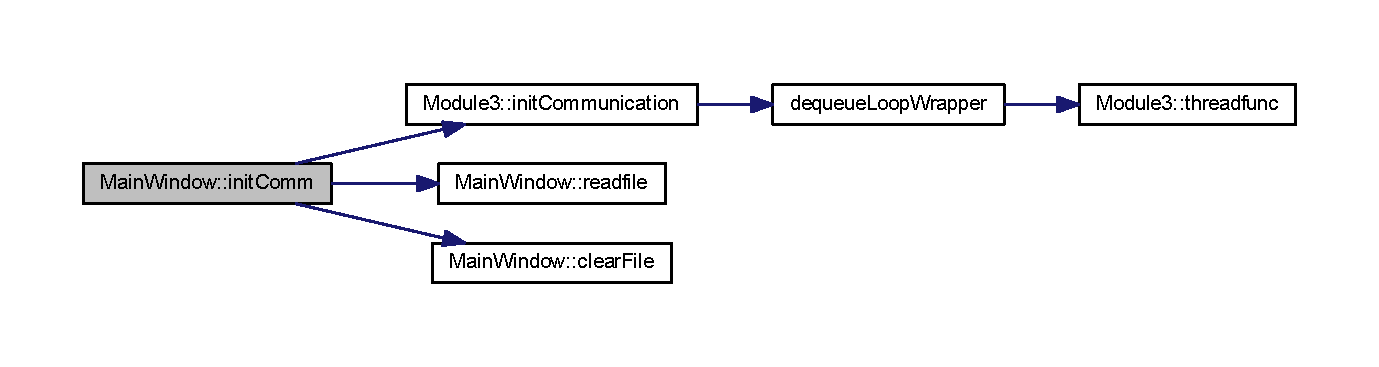
\includegraphics[width=350pt]{class_main_window_a3ae7677276119857e128f826c8b069c8_cgraph}
\end{center}
\end{figure}
\mbox{\Hypertarget{class_main_window_a88b30e72fd13b54ddef7bf6e2bb08448}\label{class_main_window_a88b30e72fd13b54ddef7bf6e2bb08448}} 
\index{Main\+Window@{Main\+Window}!insert\+Routine@{insert\+Routine}}
\index{insert\+Routine@{insert\+Routine}!Main\+Window@{Main\+Window}}
\subsubsection{\texorpdfstring{insert\+Routine}{insertRoutine}}
{\footnotesize\ttfamily void Main\+Window\+::insert\+Routine (\begin{DoxyParamCaption}{ }\end{DoxyParamCaption})\hspace{0.3cm}{\ttfamily [private]}, {\ttfamily [slot]}}

Here is the call graph for this function\+:
\nopagebreak
\begin{figure}[H]
\begin{center}
\leavevmode
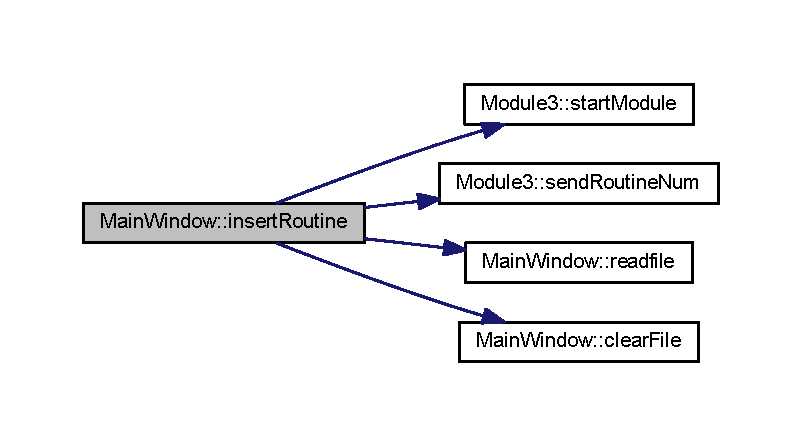
\includegraphics[width=350pt]{class_main_window_a88b30e72fd13b54ddef7bf6e2bb08448_cgraph}
\end{center}
\end{figure}
\mbox{\Hypertarget{class_main_window_aadedb5af94649f8e8a16c6642aa7b319}\label{class_main_window_aadedb5af94649f8e8a16c6642aa7b319}} 
\index{Main\+Window@{Main\+Window}!insert\+Routine\+Number@{insert\+Routine\+Number}}
\index{insert\+Routine\+Number@{insert\+Routine\+Number}!Main\+Window@{Main\+Window}}
\subsubsection{\texorpdfstring{insert\+Routine\+Number}{insertRoutineNumber}}
{\footnotesize\ttfamily void Main\+Window\+::insert\+Routine\+Number (\begin{DoxyParamCaption}{ }\end{DoxyParamCaption})\hspace{0.3cm}{\ttfamily [signal]}}

\mbox{\Hypertarget{class_main_window_a45eac78192a605f450c10b8c4b1bde81}\label{class_main_window_a45eac78192a605f450c10b8c4b1bde81}} 
\index{Main\+Window@{Main\+Window}!readfile@{readfile}}
\index{readfile@{readfile}!Main\+Window@{Main\+Window}}
\subsubsection{\texorpdfstring{readfile()}{readfile()}}
{\footnotesize\ttfamily void Main\+Window\+::readfile (\begin{DoxyParamCaption}{ }\end{DoxyParamCaption})}

\mbox{\Hypertarget{class_main_window_aab2fed34f5ba1468a0c9ff35fcd79757}\label{class_main_window_aab2fed34f5ba1468a0c9ff35fcd79757}} 
\index{Main\+Window@{Main\+Window}!terminate\+Program@{terminate\+Program}}
\index{terminate\+Program@{terminate\+Program}!Main\+Window@{Main\+Window}}
\subsubsection{\texorpdfstring{terminate\+Program}{terminateProgram}}
{\footnotesize\ttfamily void Main\+Window\+::terminate\+Program (\begin{DoxyParamCaption}{ }\end{DoxyParamCaption})\hspace{0.3cm}{\ttfamily [private]}, {\ttfamily [slot]}}

Here is the call graph for this function\+:
\nopagebreak
\begin{figure}[H]
\begin{center}
\leavevmode
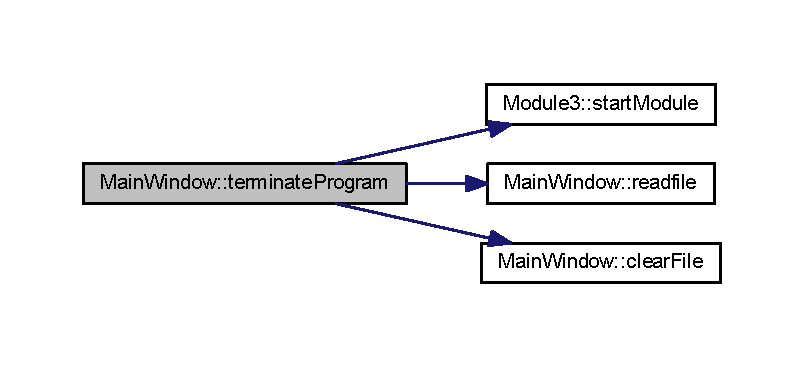
\includegraphics[width=350pt]{class_main_window_aab2fed34f5ba1468a0c9ff35fcd79757_cgraph}
\end{center}
\end{figure}


\subsection{Member Data Documentation}
\mbox{\Hypertarget{class_main_window_a9d4a6f9ce2275a736abcedf0bba2bad9}\label{class_main_window_a9d4a6f9ce2275a736abcedf0bba2bad9}} 
\index{Main\+Window@{Main\+Window}!disconnect@{disconnect}}
\index{disconnect@{disconnect}!Main\+Window@{Main\+Window}}
\subsubsection{\texorpdfstring{disconnect}{disconnect}}
{\footnotesize\ttfamily Q\+Push\+Button$\ast$ Main\+Window\+::disconnect\hspace{0.3cm}{\ttfamily [private]}}

\mbox{\Hypertarget{class_main_window_afb9e7419ea1c7c1f109857ac8ed9e703}\label{class_main_window_afb9e7419ea1c7c1f109857ac8ed9e703}} 
\index{Main\+Window@{Main\+Window}!dl\+\_\+button@{dl\+\_\+button}}
\index{dl\+\_\+button@{dl\+\_\+button}!Main\+Window@{Main\+Window}}
\subsubsection{\texorpdfstring{dl\+\_\+button}{dl\_button}}
{\footnotesize\ttfamily Q\+Push\+Button$\ast$ Main\+Window\+::dl\+\_\+button\hspace{0.3cm}{\ttfamily [private]}}

\mbox{\Hypertarget{class_main_window_a33fff3efd2a06d6df2e37219d44d9d20}\label{class_main_window_a33fff3efd2a06d6df2e37219d44d9d20}} 
\index{Main\+Window@{Main\+Window}!get\+Msg\+Q\+\_\+button@{get\+Msg\+Q\+\_\+button}}
\index{get\+Msg\+Q\+\_\+button@{get\+Msg\+Q\+\_\+button}!Main\+Window@{Main\+Window}}
\subsubsection{\texorpdfstring{get\+Msg\+Q\+\_\+button}{getMsgQ\_button}}
{\footnotesize\ttfamily Q\+Push\+Button$\ast$ Main\+Window\+::get\+Msg\+Q\+\_\+button\hspace{0.3cm}{\ttfamily [private]}}

\mbox{\Hypertarget{class_main_window_a26663544e9c5a627b73df4d060a9a06a}\label{class_main_window_a26663544e9c5a627b73df4d060a9a06a}} 
\index{Main\+Window@{Main\+Window}!get\+Sh\+Mem\+\_\+button@{get\+Sh\+Mem\+\_\+button}}
\index{get\+Sh\+Mem\+\_\+button@{get\+Sh\+Mem\+\_\+button}!Main\+Window@{Main\+Window}}
\subsubsection{\texorpdfstring{get\+Sh\+Mem\+\_\+button}{getShMem\_button}}
{\footnotesize\ttfamily Q\+Push\+Button$\ast$ Main\+Window\+::get\+Sh\+Mem\+\_\+button\hspace{0.3cm}{\ttfamily [private]}}

\mbox{\Hypertarget{class_main_window_ad1f2bbeefb0b2f010eef8fcd2f0b825f}\label{class_main_window_ad1f2bbeefb0b2f010eef8fcd2f0b825f}} 
\index{Main\+Window@{Main\+Window}!info\+Bar@{info\+Bar}}
\index{info\+Bar@{info\+Bar}!Main\+Window@{Main\+Window}}
\subsubsection{\texorpdfstring{info\+Bar}{infoBar}}
{\footnotesize\ttfamily Q\+Label$\ast$ Main\+Window\+::info\+Bar\hspace{0.3cm}{\ttfamily [private]}}

\mbox{\Hypertarget{class_main_window_ad1cf02a751bb3647114db947acebcaf5}\label{class_main_window_ad1cf02a751bb3647114db947acebcaf5}} 
\index{Main\+Window@{Main\+Window}!init\+\_\+button@{init\+\_\+button}}
\index{init\+\_\+button@{init\+\_\+button}!Main\+Window@{Main\+Window}}
\subsubsection{\texorpdfstring{init\+\_\+button}{init\_button}}
{\footnotesize\ttfamily Q\+Push\+Button$\ast$ Main\+Window\+::init\+\_\+button\hspace{0.3cm}{\ttfamily [private]}}

\mbox{\Hypertarget{class_main_window_a13d73f676f1bfdd6090677bbc17dc3bb}\label{class_main_window_a13d73f676f1bfdd6090677bbc17dc3bb}} 
\index{Main\+Window@{Main\+Window}!mod3@{mod3}}
\index{mod3@{mod3}!Main\+Window@{Main\+Window}}
\subsubsection{\texorpdfstring{mod3}{mod3}}
{\footnotesize\ttfamily \mbox{\hyperlink{class_module3}{Module3}} Main\+Window\+::mod3\hspace{0.3cm}{\ttfamily [private]}}

\mbox{\Hypertarget{class_main_window_a9f6d60a6052813c8d83a0a2b3e1c9b2a}\label{class_main_window_a9f6d60a6052813c8d83a0a2b3e1c9b2a}} 
\index{Main\+Window@{Main\+Window}!process@{process}}
\index{process@{process}!Main\+Window@{Main\+Window}}
\subsubsection{\texorpdfstring{process}{process}}
{\footnotesize\ttfamily Q\+Process$\ast$ Main\+Window\+::process\hspace{0.3cm}{\ttfamily [private]}}

\mbox{\Hypertarget{class_main_window_ab016004d1d7ba0084b7201072c2ff193}\label{class_main_window_ab016004d1d7ba0084b7201072c2ff193}} 
\index{Main\+Window@{Main\+Window}!routine\+Text@{routine\+Text}}
\index{routine\+Text@{routine\+Text}!Main\+Window@{Main\+Window}}
\subsubsection{\texorpdfstring{routine\+Text}{routineText}}
{\footnotesize\ttfamily Q\+Line\+Edit$\ast$ Main\+Window\+::routine\+Text\hspace{0.3cm}{\ttfamily [private]}}

\mbox{\Hypertarget{class_main_window_a56a195b11e21a9e73cc7adad5b4666a1}\label{class_main_window_a56a195b11e21a9e73cc7adad5b4666a1}} 
\index{Main\+Window@{Main\+Window}!send\+Routine\+\_\+button@{send\+Routine\+\_\+button}}
\index{send\+Routine\+\_\+button@{send\+Routine\+\_\+button}!Main\+Window@{Main\+Window}}
\subsubsection{\texorpdfstring{send\+Routine\+\_\+button}{sendRoutine\_button}}
{\footnotesize\ttfamily Q\+Push\+Button$\ast$ Main\+Window\+::send\+Routine\+\_\+button\hspace{0.3cm}{\ttfamily [private]}}

\mbox{\Hypertarget{class_main_window_ae1fe4774da9daef3570ef190df36773e}\label{class_main_window_ae1fe4774da9daef3570ef190df36773e}} 
\index{Main\+Window@{Main\+Window}!show\+Text@{show\+Text}}
\index{show\+Text@{show\+Text}!Main\+Window@{Main\+Window}}
\subsubsection{\texorpdfstring{show\+Text}{showText}}
{\footnotesize\ttfamily Q\+Text\+Edit$\ast$ Main\+Window\+::show\+Text\hspace{0.3cm}{\ttfamily [private]}}

\mbox{\Hypertarget{class_main_window_a98c79855a722db4582f2c1f41b0369df}\label{class_main_window_a98c79855a722db4582f2c1f41b0369df}} 
\index{Main\+Window@{Main\+Window}!text\+User@{text\+User}}
\index{text\+User@{text\+User}!Main\+Window@{Main\+Window}}
\subsubsection{\texorpdfstring{text\+User}{textUser}}
{\footnotesize\ttfamily Q\+Line\+Edit$\ast$ Main\+Window\+::text\+User\hspace{0.3cm}{\ttfamily [private]}}

\mbox{\Hypertarget{class_main_window_a35466a70ed47252a0191168126a352a5}\label{class_main_window_a35466a70ed47252a0191168126a352a5}} 
\index{Main\+Window@{Main\+Window}!ui@{ui}}
\index{ui@{ui}!Main\+Window@{Main\+Window}}
\subsubsection{\texorpdfstring{ui}{ui}}
{\footnotesize\ttfamily Ui\+::\+Main\+Window$\ast$ Main\+Window\+::ui\hspace{0.3cm}{\ttfamily [private]}}



The documentation for this class was generated from the following files\+:\begin{DoxyCompactItemize}
\item 
\mbox{\hyperlink{mainwindow_8h}{mainwindow.\+h}}\item 
\mbox{\hyperlink{mainwindow_8cpp}{mainwindow.\+cpp}}\end{DoxyCompactItemize}

\hypertarget{class_module3}{}\section{Module3 Class Reference}
\label{class_module3}\index{Module3@{Module3}}


{\ttfamily \#include $<$\+\_\+module3.\+h$>$}



Inheritance diagram for Module3\+:
\nopagebreak
\begin{figure}[H]
\begin{center}
\leavevmode
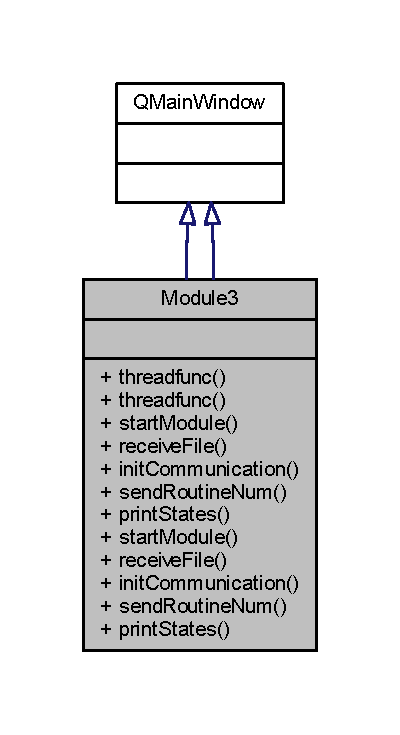
\includegraphics[width=192pt]{class_module3__inherit__graph}
\end{center}
\end{figure}


Collaboration diagram for Module3\+:
\nopagebreak
\begin{figure}[H]
\begin{center}
\leavevmode
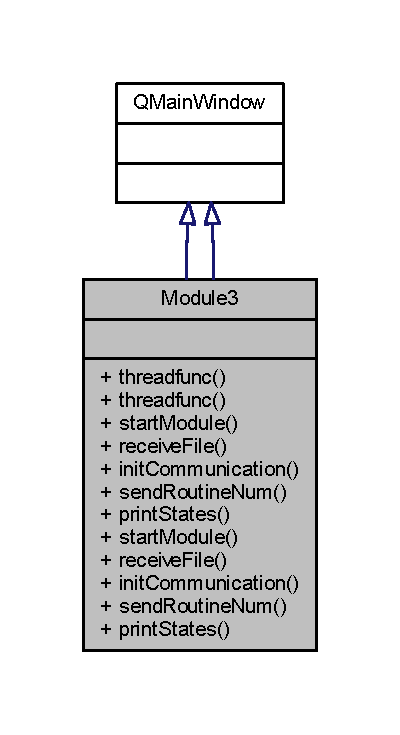
\includegraphics[width=192pt]{class_module3__coll__graph}
\end{center}
\end{figure}
\subsection*{Public Slots}
\begin{DoxyCompactItemize}
\item 
int \mbox{\hyperlink{class_module3_af03e3df56d29af941005a6c83717d8db}{start\+Module}} (int inserted\+Number)
\item 
void \mbox{\hyperlink{class_module3_a81f76e7a449ea3a014a862ec7d33498a}{receive\+File}} ()
\item 
int \mbox{\hyperlink{class_module3_ac66437d00aebddd32dc0618de74ea5a3}{init\+Communication}} (void)
\item 
void \mbox{\hyperlink{class_module3_a17b4aac26b4f9d44ec48a8022913cc7a}{send\+Routine\+Num}} (int r\+Num)
\item 
void \mbox{\hyperlink{class_module3_ac91b756cb9b50b0d7e2e177823baad48}{print\+States}} (void)
\item 
int \mbox{\hyperlink{class_module3_af03e3df56d29af941005a6c83717d8db}{start\+Module}} (int inserted\+Number)
\item 
void \mbox{\hyperlink{class_module3_a81f76e7a449ea3a014a862ec7d33498a}{receive\+File}} ()
\item 
void \mbox{\hyperlink{class_module3_ac66437d00aebddd32dc0618de74ea5a3}{init\+Communication}} (void)
\item 
void \mbox{\hyperlink{class_module3_a17b4aac26b4f9d44ec48a8022913cc7a}{send\+Routine\+Num}} (int r\+Num)
\item 
void \mbox{\hyperlink{class_module3_ac91b756cb9b50b0d7e2e177823baad48}{print\+States}} (void)
\end{DoxyCompactItemize}
\subsection*{Signals}
\begin{DoxyCompactItemize}
\item 
void \mbox{\hyperlink{class_module3_a2fee494b81b29cb56c1d860a5306adf2}{insert\+Number}} ()
\item 
void \mbox{\hyperlink{class_module3_ab15973c4f5ceb61037de263982e3989a}{print\+Receiving}} ()
\item 
void \mbox{\hyperlink{class_module3_a2fee494b81b29cb56c1d860a5306adf2}{insert\+Number}} ()
\item 
void \mbox{\hyperlink{class_module3_ab15973c4f5ceb61037de263982e3989a}{print\+Receiving}} ()
\end{DoxyCompactItemize}
\subsection*{Public Member Functions}
\begin{DoxyCompactItemize}
\item 
void $\ast$ \mbox{\hyperlink{class_module3_a21e8c133eee38224201d9826a6b08894}{threadfunc}} (void $\ast$arg)
\item 
void $\ast$ \mbox{\hyperlink{class_module3_a38ac22b1c247687546a3b27dffc8e26a}{threadfunc}} (void $\ast$arg)
\end{DoxyCompactItemize}


\subsection{Member Function Documentation}
\mbox{\Hypertarget{class_module3_ac66437d00aebddd32dc0618de74ea5a3}\label{class_module3_ac66437d00aebddd32dc0618de74ea5a3}} 
\index{Module3@{Module3}!init\+Communication@{init\+Communication}}
\index{init\+Communication@{init\+Communication}!Module3@{Module3}}
\subsubsection{\texorpdfstring{init\+Communication}{initCommunication}\hspace{0.1cm}{\footnotesize\ttfamily [1/2]}}
{\footnotesize\ttfamily void Module3\+::init\+Communication (\begin{DoxyParamCaption}\item[{void}]{ }\end{DoxyParamCaption})\hspace{0.3cm}{\ttfamily [slot]}}

Here is the call graph for this function\+:
\nopagebreak
\begin{figure}[H]
\begin{center}
\leavevmode
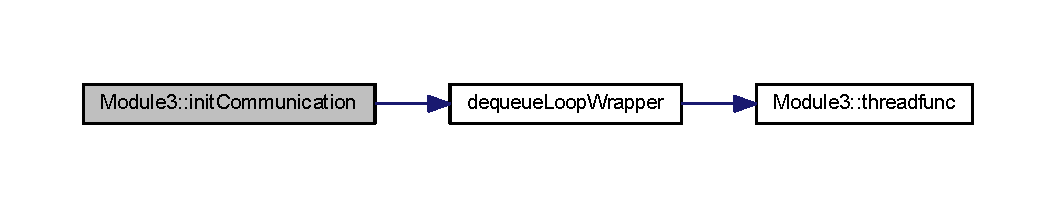
\includegraphics[width=350pt]{class_module3_ac66437d00aebddd32dc0618de74ea5a3_cgraph}
\end{center}
\end{figure}
\mbox{\Hypertarget{class_module3_ac66437d00aebddd32dc0618de74ea5a3}\label{class_module3_ac66437d00aebddd32dc0618de74ea5a3}} 
\index{Module3@{Module3}!init\+Communication@{init\+Communication}}
\index{init\+Communication@{init\+Communication}!Module3@{Module3}}
\subsubsection{\texorpdfstring{init\+Communication}{initCommunication}\hspace{0.1cm}{\footnotesize\ttfamily [2/2]}}
{\footnotesize\ttfamily void Module3\+::init\+Communication (\begin{DoxyParamCaption}\item[{void}]{ }\end{DoxyParamCaption})\hspace{0.3cm}{\ttfamily [slot]}}

\mbox{\Hypertarget{class_module3_a2fee494b81b29cb56c1d860a5306adf2}\label{class_module3_a2fee494b81b29cb56c1d860a5306adf2}} 
\index{Module3@{Module3}!insert\+Number@{insert\+Number}}
\index{insert\+Number@{insert\+Number}!Module3@{Module3}}
\subsubsection{\texorpdfstring{insert\+Number}{insertNumber}\hspace{0.1cm}{\footnotesize\ttfamily [1/2]}}
{\footnotesize\ttfamily void Module3\+::insert\+Number (\begin{DoxyParamCaption}{ }\end{DoxyParamCaption})\hspace{0.3cm}{\ttfamily [signal]}}

\mbox{\Hypertarget{class_module3_a2fee494b81b29cb56c1d860a5306adf2}\label{class_module3_a2fee494b81b29cb56c1d860a5306adf2}} 
\index{Module3@{Module3}!insert\+Number@{insert\+Number}}
\index{insert\+Number@{insert\+Number}!Module3@{Module3}}
\subsubsection{\texorpdfstring{insert\+Number}{insertNumber}\hspace{0.1cm}{\footnotesize\ttfamily [2/2]}}
{\footnotesize\ttfamily void Module3\+::insert\+Number (\begin{DoxyParamCaption}{ }\end{DoxyParamCaption})\hspace{0.3cm}{\ttfamily [signal]}}

\mbox{\Hypertarget{class_module3_ab15973c4f5ceb61037de263982e3989a}\label{class_module3_ab15973c4f5ceb61037de263982e3989a}} 
\index{Module3@{Module3}!print\+Receiving@{print\+Receiving}}
\index{print\+Receiving@{print\+Receiving}!Module3@{Module3}}
\subsubsection{\texorpdfstring{print\+Receiving}{printReceiving}\hspace{0.1cm}{\footnotesize\ttfamily [1/2]}}
{\footnotesize\ttfamily void Module3\+::print\+Receiving (\begin{DoxyParamCaption}{ }\end{DoxyParamCaption})\hspace{0.3cm}{\ttfamily [signal]}}

\mbox{\Hypertarget{class_module3_ab15973c4f5ceb61037de263982e3989a}\label{class_module3_ab15973c4f5ceb61037de263982e3989a}} 
\index{Module3@{Module3}!print\+Receiving@{print\+Receiving}}
\index{print\+Receiving@{print\+Receiving}!Module3@{Module3}}
\subsubsection{\texorpdfstring{print\+Receiving}{printReceiving}\hspace{0.1cm}{\footnotesize\ttfamily [2/2]}}
{\footnotesize\ttfamily void Module3\+::print\+Receiving (\begin{DoxyParamCaption}{ }\end{DoxyParamCaption})\hspace{0.3cm}{\ttfamily [signal]}}

\mbox{\Hypertarget{class_module3_ac91b756cb9b50b0d7e2e177823baad48}\label{class_module3_ac91b756cb9b50b0d7e2e177823baad48}} 
\index{Module3@{Module3}!print\+States@{print\+States}}
\index{print\+States@{print\+States}!Module3@{Module3}}
\subsubsection{\texorpdfstring{print\+States}{printStates}\hspace{0.1cm}{\footnotesize\ttfamily [1/2]}}
{\footnotesize\ttfamily void Module3\+::print\+States (\begin{DoxyParamCaption}\item[{void}]{ }\end{DoxyParamCaption})\hspace{0.3cm}{\ttfamily [slot]}}

\mbox{\Hypertarget{class_module3_ac91b756cb9b50b0d7e2e177823baad48}\label{class_module3_ac91b756cb9b50b0d7e2e177823baad48}} 
\index{Module3@{Module3}!print\+States@{print\+States}}
\index{print\+States@{print\+States}!Module3@{Module3}}
\subsubsection{\texorpdfstring{print\+States}{printStates}\hspace{0.1cm}{\footnotesize\ttfamily [2/2]}}
{\footnotesize\ttfamily void Module3\+::print\+States (\begin{DoxyParamCaption}\item[{void}]{ }\end{DoxyParamCaption})\hspace{0.3cm}{\ttfamily [slot]}}

\mbox{\Hypertarget{class_module3_a81f76e7a449ea3a014a862ec7d33498a}\label{class_module3_a81f76e7a449ea3a014a862ec7d33498a}} 
\index{Module3@{Module3}!receive\+File@{receive\+File}}
\index{receive\+File@{receive\+File}!Module3@{Module3}}
\subsubsection{\texorpdfstring{receive\+File}{receiveFile}\hspace{0.1cm}{\footnotesize\ttfamily [1/2]}}
{\footnotesize\ttfamily void Module3\+::receive\+File (\begin{DoxyParamCaption}{ }\end{DoxyParamCaption})\hspace{0.3cm}{\ttfamily [slot]}}

\mbox{\Hypertarget{class_module3_a81f76e7a449ea3a014a862ec7d33498a}\label{class_module3_a81f76e7a449ea3a014a862ec7d33498a}} 
\index{Module3@{Module3}!receive\+File@{receive\+File}}
\index{receive\+File@{receive\+File}!Module3@{Module3}}
\subsubsection{\texorpdfstring{receive\+File}{receiveFile}\hspace{0.1cm}{\footnotesize\ttfamily [2/2]}}
{\footnotesize\ttfamily void Module3\+::receive\+File (\begin{DoxyParamCaption}{ }\end{DoxyParamCaption})\hspace{0.3cm}{\ttfamily [slot]}}

\mbox{\Hypertarget{class_module3_a17b4aac26b4f9d44ec48a8022913cc7a}\label{class_module3_a17b4aac26b4f9d44ec48a8022913cc7a}} 
\index{Module3@{Module3}!send\+Routine\+Num@{send\+Routine\+Num}}
\index{send\+Routine\+Num@{send\+Routine\+Num}!Module3@{Module3}}
\subsubsection{\texorpdfstring{send\+Routine\+Num}{sendRoutineNum}\hspace{0.1cm}{\footnotesize\ttfamily [1/2]}}
{\footnotesize\ttfamily void Module3\+::send\+Routine\+Num (\begin{DoxyParamCaption}\item[{int}]{r\+Num }\end{DoxyParamCaption})\hspace{0.3cm}{\ttfamily [slot]}}

\mbox{\Hypertarget{class_module3_a17b4aac26b4f9d44ec48a8022913cc7a}\label{class_module3_a17b4aac26b4f9d44ec48a8022913cc7a}} 
\index{Module3@{Module3}!send\+Routine\+Num@{send\+Routine\+Num}}
\index{send\+Routine\+Num@{send\+Routine\+Num}!Module3@{Module3}}
\subsubsection{\texorpdfstring{send\+Routine\+Num}{sendRoutineNum}\hspace{0.1cm}{\footnotesize\ttfamily [2/2]}}
{\footnotesize\ttfamily void Module3\+::send\+Routine\+Num (\begin{DoxyParamCaption}\item[{int}]{r\+Num }\end{DoxyParamCaption})\hspace{0.3cm}{\ttfamily [slot]}}

\mbox{\Hypertarget{class_module3_af03e3df56d29af941005a6c83717d8db}\label{class_module3_af03e3df56d29af941005a6c83717d8db}} 
\index{Module3@{Module3}!start\+Module@{start\+Module}}
\index{start\+Module@{start\+Module}!Module3@{Module3}}
\subsubsection{\texorpdfstring{start\+Module}{startModule}\hspace{0.1cm}{\footnotesize\ttfamily [1/2]}}
{\footnotesize\ttfamily int Module3\+::start\+Module (\begin{DoxyParamCaption}\item[{int}]{inserted\+Number }\end{DoxyParamCaption})\hspace{0.3cm}{\ttfamily [slot]}}

\mbox{\Hypertarget{class_module3_af03e3df56d29af941005a6c83717d8db}\label{class_module3_af03e3df56d29af941005a6c83717d8db}} 
\index{Module3@{Module3}!start\+Module@{start\+Module}}
\index{start\+Module@{start\+Module}!Module3@{Module3}}
\subsubsection{\texorpdfstring{start\+Module}{startModule}\hspace{0.1cm}{\footnotesize\ttfamily [2/2]}}
{\footnotesize\ttfamily int Module3\+::start\+Module (\begin{DoxyParamCaption}\item[{int}]{inserted\+Number }\end{DoxyParamCaption})\hspace{0.3cm}{\ttfamily [slot]}}

\mbox{\Hypertarget{class_module3_a21e8c133eee38224201d9826a6b08894}\label{class_module3_a21e8c133eee38224201d9826a6b08894}} 
\index{Module3@{Module3}!threadfunc@{threadfunc}}
\index{threadfunc@{threadfunc}!Module3@{Module3}}
\subsubsection{\texorpdfstring{threadfunc()}{threadfunc()}\hspace{0.1cm}{\footnotesize\ttfamily [1/2]}}
{\footnotesize\ttfamily void $\ast$ Module3\+::threadfunc (\begin{DoxyParamCaption}\item[{void $\ast$}]{arg }\end{DoxyParamCaption})}

\mbox{\Hypertarget{class_module3_a38ac22b1c247687546a3b27dffc8e26a}\label{class_module3_a38ac22b1c247687546a3b27dffc8e26a}} 
\index{Module3@{Module3}!threadfunc@{threadfunc}}
\index{threadfunc@{threadfunc}!Module3@{Module3}}
\subsubsection{\texorpdfstring{threadfunc()}{threadfunc()}\hspace{0.1cm}{\footnotesize\ttfamily [2/2]}}
{\footnotesize\ttfamily void$\ast$ Module3\+::threadfunc (\begin{DoxyParamCaption}\item[{void $\ast$}]{arg }\end{DoxyParamCaption})}



The documentation for this class was generated from the following files\+:\begin{DoxyCompactItemize}
\item 
\mbox{\hyperlink{__module3_8h}{\+\_\+module3.\+h}}\item 
\mbox{\hyperlink{module3_8h}{module3.\+h}}\item 
\mbox{\hyperlink{module3_8cpp}{module3.\+cpp}}\end{DoxyCompactItemize}

\hypertarget{class_q_main_window}{}\section{Q\+Main\+Window Class Reference}
\label{class_q_main_window}\index{Q\+Main\+Window@{Q\+Main\+Window}}


Inheritance diagram for Q\+Main\+Window\+:
\nopagebreak
\begin{figure}[H]
\begin{center}
\leavevmode
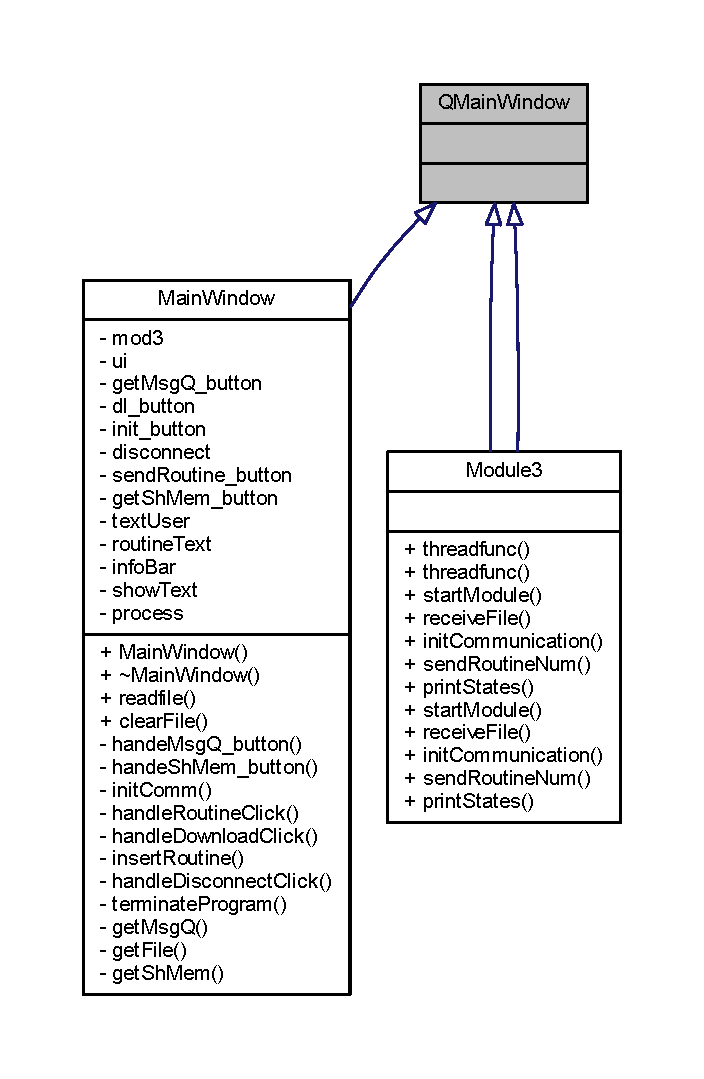
\includegraphics[width=338pt]{class_q_main_window__inherit__graph}
\end{center}
\end{figure}


Collaboration diagram for Q\+Main\+Window\+:
\nopagebreak
\begin{figure}[H]
\begin{center}
\leavevmode
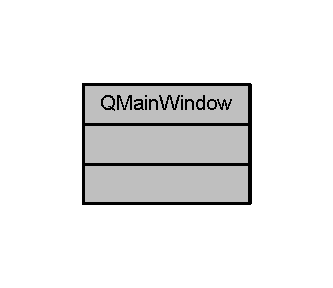
\includegraphics[width=160pt]{class_q_main_window__coll__graph}
\end{center}
\end{figure}


The documentation for this class was generated from the following file\+:\begin{DoxyCompactItemize}
\item 
\mbox{\hyperlink{module3_8h}{module3.\+h}}\end{DoxyCompactItemize}

\chapter{File Documentation}
\hypertarget{__module3_8h}{}\section{\+\_\+module3.\+h File Reference}
\label{__module3_8h}\index{\+\_\+module3.\+h@{\+\_\+module3.\+h}}
{\ttfamily \#include $<$Q\+Main\+Window$>$}\newline
{\ttfamily \#include $<$Q\+Line\+Edit$>$}\newline
{\ttfamily \#include $<$Q\+File$>$}\newline
{\ttfamily \#include $<$Q\+Debug$>$}\newline
{\ttfamily \#include $<$Q\+Text\+Edit$>$}\newline
Include dependency graph for \+\_\+module3.\+h\+:
\nopagebreak
\begin{figure}[H]
\begin{center}
\leavevmode
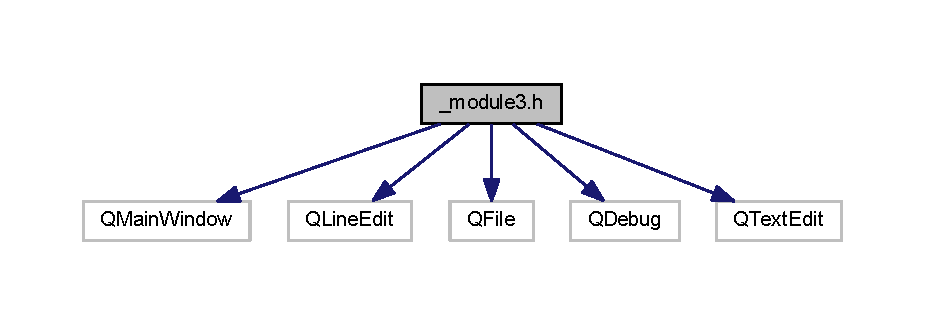
\includegraphics[width=350pt]{__module3_8h__incl}
\end{center}
\end{figure}
\subsection*{Classes}
\begin{DoxyCompactItemize}
\item 
struct \mbox{\hyperlink{structerror_struct}{error\+Struct}}
\item 
struct \mbox{\hyperlink{structdiagnostic_data_msg_q}{diagnostic\+Data\+MsgQ}}
\item 
struct \mbox{\hyperlink{structdiagnostic_data_sh_m}{diagnostic\+Data\+ShM}}
\item 
class \mbox{\hyperlink{class_module3}{Module3}}
\end{DoxyCompactItemize}
\subsection*{Namespaces}
\begin{DoxyCompactItemize}
\item 
 \mbox{\hyperlink{namespace_ui}{Ui}}
\end{DoxyCompactItemize}
\subsection*{Macros}
\begin{DoxyCompactItemize}
\item 
\#define \mbox{\hyperlink{__module3_8h_adfc8f90f3a8caa8423099cf36ff214f1}{\+\_\+\+W\+I\+N\+S\+O\+C\+K\+\_\+\+D\+E\+P\+R\+E\+C\+A\+T\+E\+D\+\_\+\+N\+O\+\_\+\+W\+A\+R\+N\+I\+N\+GS}}
\item 
\#define \mbox{\hyperlink{__module3_8h_abe0b7b2a0ec4b64b92585808a051e1fa}{S\+L\+E\+E\+P\+\_\+\+T\+I\+ME}}~15
\item 
\#define \mbox{\hyperlink{__module3_8h_afd8807aef011a7518ea028a4d29ebd4a}{S\+W\+U\+\_\+\+B\+R\+\_\+\+S\+E\+R\+V\+E\+R\+P\+O\+RT}}~29170
\item 
\#define \mbox{\hyperlink{__module3_8h_ab3570d75ac730a357320f9d5dae2c884}{S\+W\+U\+\_\+\+B\+R\+\_\+\+C\+L\+I\+E\+N\+T\+P\+O\+RT}}~29171
\item 
\#define \mbox{\hyperlink{__module3_8h_ad974fe981249f5e84fbf1683b012c9f8}{B\+U\+F\+L\+EN}}~512
\item 
\#define \mbox{\hyperlink{__module3_8h_aca9322dca2cb4e10ba445ecf867885c1}{z\+F\+A\+S\+\_\+\+I\+Pv4}}~\char`\"{}192.\+168.\+122.\+60\char`\"{}
\end{DoxyCompactItemize}
\subsection*{Typedefs}
\begin{DoxyCompactItemize}
\item 
typedef struct \mbox{\hyperlink{structerror_struct}{error\+Struct}} \mbox{\hyperlink{__module3_8h_aed782b3a5727361a6b656be14d539f9c}{s\+\_\+\+E\+R\+R\+O\+RS}}
\item 
typedef struct \mbox{\hyperlink{structdiagnostic_data_msg_q}{diagnostic\+Data\+MsgQ}} \mbox{\hyperlink{__module3_8h_a58c449f6052675fb4288c20122741cb8}{s\+\_\+\+D\+I\+A\+G\+\_\+\+D\+A\+TA}}
\item 
typedef struct \mbox{\hyperlink{structdiagnostic_data_sh_m}{diagnostic\+Data\+ShM}} \mbox{\hyperlink{__module3_8h_a1f542cc6438c66026963a340365d442a}{s\+\_\+\+D\+I\+A\+G\+\_\+\+S\+H\+M\+\_\+\+D\+A\+TA}}
\end{DoxyCompactItemize}


\subsection{Macro Definition Documentation}
\mbox{\Hypertarget{__module3_8h_adfc8f90f3a8caa8423099cf36ff214f1}\label{__module3_8h_adfc8f90f3a8caa8423099cf36ff214f1}} 
\index{\+\_\+module3.\+h@{\+\_\+module3.\+h}!\+\_\+\+W\+I\+N\+S\+O\+C\+K\+\_\+\+D\+E\+P\+R\+E\+C\+A\+T\+E\+D\+\_\+\+N\+O\+\_\+\+W\+A\+R\+N\+I\+N\+GS@{\+\_\+\+W\+I\+N\+S\+O\+C\+K\+\_\+\+D\+E\+P\+R\+E\+C\+A\+T\+E\+D\+\_\+\+N\+O\+\_\+\+W\+A\+R\+N\+I\+N\+GS}}
\index{\+\_\+\+W\+I\+N\+S\+O\+C\+K\+\_\+\+D\+E\+P\+R\+E\+C\+A\+T\+E\+D\+\_\+\+N\+O\+\_\+\+W\+A\+R\+N\+I\+N\+GS@{\+\_\+\+W\+I\+N\+S\+O\+C\+K\+\_\+\+D\+E\+P\+R\+E\+C\+A\+T\+E\+D\+\_\+\+N\+O\+\_\+\+W\+A\+R\+N\+I\+N\+GS}!\+\_\+module3.\+h@{\+\_\+module3.\+h}}
\subsubsection{\texorpdfstring{\+\_\+\+W\+I\+N\+S\+O\+C\+K\+\_\+\+D\+E\+P\+R\+E\+C\+A\+T\+E\+D\+\_\+\+N\+O\+\_\+\+W\+A\+R\+N\+I\+N\+GS}{\_WINSOCK\_DEPRECATED\_NO\_WARNINGS}}
{\footnotesize\ttfamily \#define \+\_\+\+W\+I\+N\+S\+O\+C\+K\+\_\+\+D\+E\+P\+R\+E\+C\+A\+T\+E\+D\+\_\+\+N\+O\+\_\+\+W\+A\+R\+N\+I\+N\+GS}

\mbox{\Hypertarget{__module3_8h_ad974fe981249f5e84fbf1683b012c9f8}\label{__module3_8h_ad974fe981249f5e84fbf1683b012c9f8}} 
\index{\+\_\+module3.\+h@{\+\_\+module3.\+h}!B\+U\+F\+L\+EN@{B\+U\+F\+L\+EN}}
\index{B\+U\+F\+L\+EN@{B\+U\+F\+L\+EN}!\+\_\+module3.\+h@{\+\_\+module3.\+h}}
\subsubsection{\texorpdfstring{B\+U\+F\+L\+EN}{BUFLEN}}
{\footnotesize\ttfamily \#define B\+U\+F\+L\+EN~512}

\mbox{\Hypertarget{__module3_8h_abe0b7b2a0ec4b64b92585808a051e1fa}\label{__module3_8h_abe0b7b2a0ec4b64b92585808a051e1fa}} 
\index{\+\_\+module3.\+h@{\+\_\+module3.\+h}!S\+L\+E\+E\+P\+\_\+\+T\+I\+ME@{S\+L\+E\+E\+P\+\_\+\+T\+I\+ME}}
\index{S\+L\+E\+E\+P\+\_\+\+T\+I\+ME@{S\+L\+E\+E\+P\+\_\+\+T\+I\+ME}!\+\_\+module3.\+h@{\+\_\+module3.\+h}}
\subsubsection{\texorpdfstring{S\+L\+E\+E\+P\+\_\+\+T\+I\+ME}{SLEEP\_TIME}}
{\footnotesize\ttfamily \#define S\+L\+E\+E\+P\+\_\+\+T\+I\+ME~15}

\mbox{\Hypertarget{__module3_8h_ab3570d75ac730a357320f9d5dae2c884}\label{__module3_8h_ab3570d75ac730a357320f9d5dae2c884}} 
\index{\+\_\+module3.\+h@{\+\_\+module3.\+h}!S\+W\+U\+\_\+\+B\+R\+\_\+\+C\+L\+I\+E\+N\+T\+P\+O\+RT@{S\+W\+U\+\_\+\+B\+R\+\_\+\+C\+L\+I\+E\+N\+T\+P\+O\+RT}}
\index{S\+W\+U\+\_\+\+B\+R\+\_\+\+C\+L\+I\+E\+N\+T\+P\+O\+RT@{S\+W\+U\+\_\+\+B\+R\+\_\+\+C\+L\+I\+E\+N\+T\+P\+O\+RT}!\+\_\+module3.\+h@{\+\_\+module3.\+h}}
\subsubsection{\texorpdfstring{S\+W\+U\+\_\+\+B\+R\+\_\+\+C\+L\+I\+E\+N\+T\+P\+O\+RT}{SWU\_BR\_CLIENTPORT}}
{\footnotesize\ttfamily \#define S\+W\+U\+\_\+\+B\+R\+\_\+\+C\+L\+I\+E\+N\+T\+P\+O\+RT~29171}

\mbox{\Hypertarget{__module3_8h_afd8807aef011a7518ea028a4d29ebd4a}\label{__module3_8h_afd8807aef011a7518ea028a4d29ebd4a}} 
\index{\+\_\+module3.\+h@{\+\_\+module3.\+h}!S\+W\+U\+\_\+\+B\+R\+\_\+\+S\+E\+R\+V\+E\+R\+P\+O\+RT@{S\+W\+U\+\_\+\+B\+R\+\_\+\+S\+E\+R\+V\+E\+R\+P\+O\+RT}}
\index{S\+W\+U\+\_\+\+B\+R\+\_\+\+S\+E\+R\+V\+E\+R\+P\+O\+RT@{S\+W\+U\+\_\+\+B\+R\+\_\+\+S\+E\+R\+V\+E\+R\+P\+O\+RT}!\+\_\+module3.\+h@{\+\_\+module3.\+h}}
\subsubsection{\texorpdfstring{S\+W\+U\+\_\+\+B\+R\+\_\+\+S\+E\+R\+V\+E\+R\+P\+O\+RT}{SWU\_BR\_SERVERPORT}}
{\footnotesize\ttfamily \#define S\+W\+U\+\_\+\+B\+R\+\_\+\+S\+E\+R\+V\+E\+R\+P\+O\+RT~29170}

\mbox{\Hypertarget{__module3_8h_aca9322dca2cb4e10ba445ecf867885c1}\label{__module3_8h_aca9322dca2cb4e10ba445ecf867885c1}} 
\index{\+\_\+module3.\+h@{\+\_\+module3.\+h}!z\+F\+A\+S\+\_\+\+I\+Pv4@{z\+F\+A\+S\+\_\+\+I\+Pv4}}
\index{z\+F\+A\+S\+\_\+\+I\+Pv4@{z\+F\+A\+S\+\_\+\+I\+Pv4}!\+\_\+module3.\+h@{\+\_\+module3.\+h}}
\subsubsection{\texorpdfstring{z\+F\+A\+S\+\_\+\+I\+Pv4}{zFAS\_IPv4}}
{\footnotesize\ttfamily \#define z\+F\+A\+S\+\_\+\+I\+Pv4~\char`\"{}192.\+168.\+122.\+60\char`\"{}}



\subsection{Typedef Documentation}
\mbox{\Hypertarget{__module3_8h_a58c449f6052675fb4288c20122741cb8}\label{__module3_8h_a58c449f6052675fb4288c20122741cb8}} 
\index{\+\_\+module3.\+h@{\+\_\+module3.\+h}!s\+\_\+\+D\+I\+A\+G\+\_\+\+D\+A\+TA@{s\+\_\+\+D\+I\+A\+G\+\_\+\+D\+A\+TA}}
\index{s\+\_\+\+D\+I\+A\+G\+\_\+\+D\+A\+TA@{s\+\_\+\+D\+I\+A\+G\+\_\+\+D\+A\+TA}!\+\_\+module3.\+h@{\+\_\+module3.\+h}}
\subsubsection{\texorpdfstring{s\+\_\+\+D\+I\+A\+G\+\_\+\+D\+A\+TA}{s\_DIAG\_DATA}}
{\footnotesize\ttfamily typedef struct \mbox{\hyperlink{structdiagnostic_data_msg_q}{diagnostic\+Data\+MsgQ}}  \mbox{\hyperlink{__module3_8h_a58c449f6052675fb4288c20122741cb8}{s\+\_\+\+D\+I\+A\+G\+\_\+\+D\+A\+TA}}}

\mbox{\Hypertarget{__module3_8h_a1f542cc6438c66026963a340365d442a}\label{__module3_8h_a1f542cc6438c66026963a340365d442a}} 
\index{\+\_\+module3.\+h@{\+\_\+module3.\+h}!s\+\_\+\+D\+I\+A\+G\+\_\+\+S\+H\+M\+\_\+\+D\+A\+TA@{s\+\_\+\+D\+I\+A\+G\+\_\+\+S\+H\+M\+\_\+\+D\+A\+TA}}
\index{s\+\_\+\+D\+I\+A\+G\+\_\+\+S\+H\+M\+\_\+\+D\+A\+TA@{s\+\_\+\+D\+I\+A\+G\+\_\+\+S\+H\+M\+\_\+\+D\+A\+TA}!\+\_\+module3.\+h@{\+\_\+module3.\+h}}
\subsubsection{\texorpdfstring{s\+\_\+\+D\+I\+A\+G\+\_\+\+S\+H\+M\+\_\+\+D\+A\+TA}{s\_DIAG\_SHM\_DATA}}
{\footnotesize\ttfamily typedef struct \mbox{\hyperlink{structdiagnostic_data_sh_m}{diagnostic\+Data\+ShM}}  \mbox{\hyperlink{__module3_8h_a1f542cc6438c66026963a340365d442a}{s\+\_\+\+D\+I\+A\+G\+\_\+\+S\+H\+M\+\_\+\+D\+A\+TA}}}

\mbox{\Hypertarget{__module3_8h_aed782b3a5727361a6b656be14d539f9c}\label{__module3_8h_aed782b3a5727361a6b656be14d539f9c}} 
\index{\+\_\+module3.\+h@{\+\_\+module3.\+h}!s\+\_\+\+E\+R\+R\+O\+RS@{s\+\_\+\+E\+R\+R\+O\+RS}}
\index{s\+\_\+\+E\+R\+R\+O\+RS@{s\+\_\+\+E\+R\+R\+O\+RS}!\+\_\+module3.\+h@{\+\_\+module3.\+h}}
\subsubsection{\texorpdfstring{s\+\_\+\+E\+R\+R\+O\+RS}{s\_ERRORS}}
{\footnotesize\ttfamily typedef struct \mbox{\hyperlink{structerror_struct}{error\+Struct}} \mbox{\hyperlink{__module3_8h_aed782b3a5727361a6b656be14d539f9c}{s\+\_\+\+E\+R\+R\+O\+RS}}}


\hypertarget{main_8cpp}{}\section{main.\+cpp File Reference}
\label{main_8cpp}\index{main.\+cpp@{main.\+cpp}}
{\ttfamily \#include \char`\"{}mainwindow.\+h\char`\"{}}\newline
{\ttfamily \#include $<$Q\+Application$>$}\newline
Include dependency graph for main.\+cpp\+:
\nopagebreak
\begin{figure}[H]
\begin{center}
\leavevmode
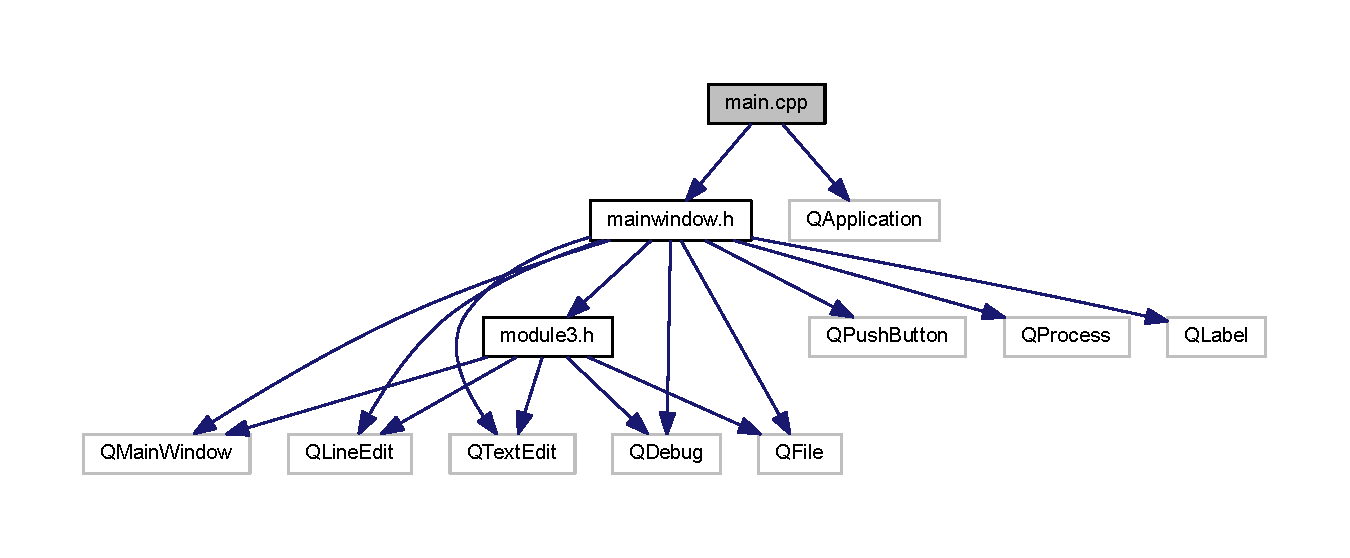
\includegraphics[width=350pt]{main_8cpp__incl}
\end{center}
\end{figure}
\subsection*{Functions}
\begin{DoxyCompactItemize}
\item 
int \mbox{\hyperlink{main_8cpp_a0ddf1224851353fc92bfbff6f499fa97}{main}} (int argc, char $\ast$argv\mbox{[}$\,$\mbox{]})
\end{DoxyCompactItemize}


\subsection{Function Documentation}
\mbox{\Hypertarget{main_8cpp_a0ddf1224851353fc92bfbff6f499fa97}\label{main_8cpp_a0ddf1224851353fc92bfbff6f499fa97}} 
\index{main.\+cpp@{main.\+cpp}!main@{main}}
\index{main@{main}!main.\+cpp@{main.\+cpp}}
\subsubsection{\texorpdfstring{main()}{main()}}
{\footnotesize\ttfamily int main (\begin{DoxyParamCaption}\item[{int}]{argc,  }\item[{char $\ast$}]{argv\mbox{[}$\,$\mbox{]} }\end{DoxyParamCaption})}


\hypertarget{mainwindow_8cpp}{}\section{mainwindow.\+cpp File Reference}
\label{mainwindow_8cpp}\index{mainwindow.\+cpp@{mainwindow.\+cpp}}
{\ttfamily \#include \char`\"{}mainwindow.\+h\char`\"{}}\newline
{\ttfamily \#include \char`\"{}ui\+\_\+mainwindow.\+h\char`\"{}}\newline
{\ttfamily \#include $<$iostream$>$}\newline
Include dependency graph for mainwindow.\+cpp\+:
\nopagebreak
\begin{figure}[H]
\begin{center}
\leavevmode
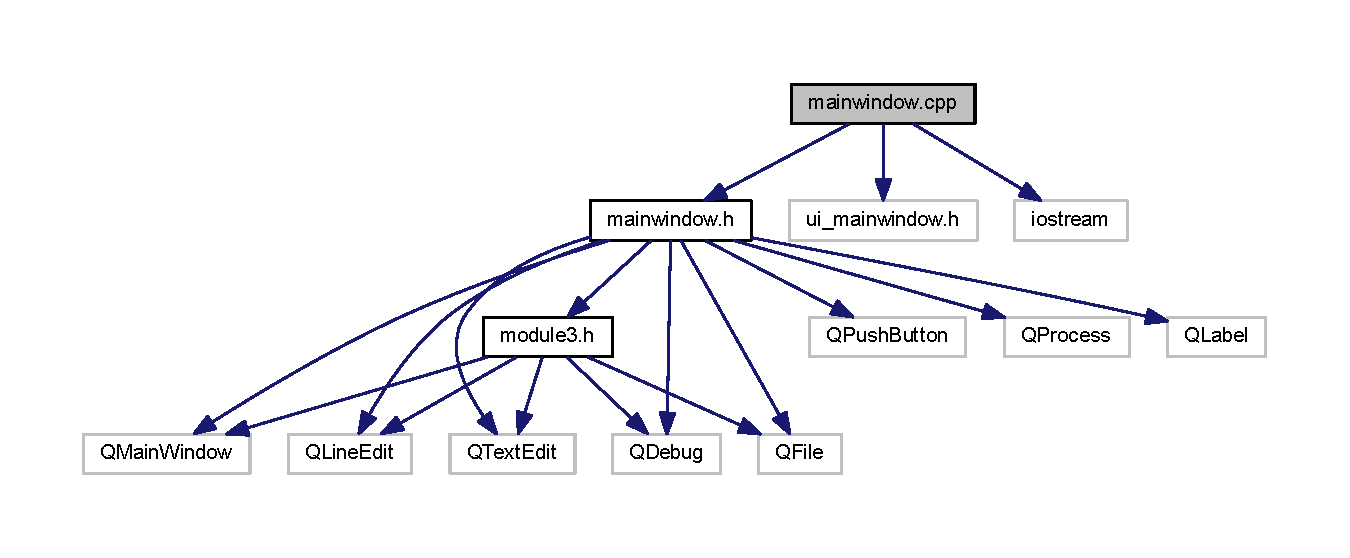
\includegraphics[width=350pt]{mainwindow_8cpp__incl}
\end{center}
\end{figure}

\hypertarget{mainwindow_8h}{}\section{mainwindow.\+h File Reference}
\label{mainwindow_8h}\index{mainwindow.\+h@{mainwindow.\+h}}
{\ttfamily \#include $<$Q\+Main\+Window$>$}\newline
{\ttfamily \#include $<$Q\+Push\+Button$>$}\newline
{\ttfamily \#include $<$Q\+Line\+Edit$>$}\newline
{\ttfamily \#include $<$Q\+Text\+Edit$>$}\newline
{\ttfamily \#include $<$Q\+Process$>$}\newline
{\ttfamily \#include $<$Q\+Debug$>$}\newline
{\ttfamily \#include $<$Q\+File$>$}\newline
{\ttfamily \#include $<$Q\+Label$>$}\newline
{\ttfamily \#include \char`\"{}module3.\+h\char`\"{}}\newline
Include dependency graph for mainwindow.\+h\+:
\nopagebreak
\begin{figure}[H]
\begin{center}
\leavevmode
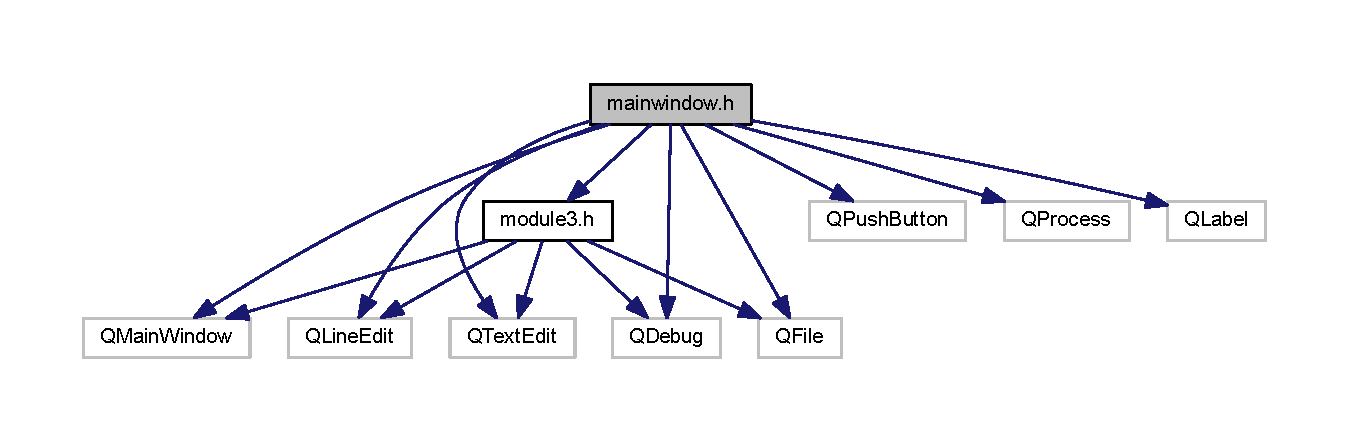
\includegraphics[width=350pt]{mainwindow_8h__incl}
\end{center}
\end{figure}
This graph shows which files directly or indirectly include this file\+:
\nopagebreak
\begin{figure}[H]
\begin{center}
\leavevmode
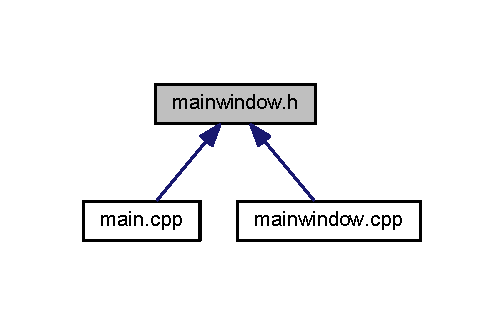
\includegraphics[width=242pt]{mainwindow_8h__dep__incl}
\end{center}
\end{figure}
\subsection*{Classes}
\begin{DoxyCompactItemize}
\item 
class \mbox{\hyperlink{class_main_window}{Main\+Window}}
\end{DoxyCompactItemize}
\subsection*{Namespaces}
\begin{DoxyCompactItemize}
\item 
 \mbox{\hyperlink{namespace_ui}{Ui}}
\end{DoxyCompactItemize}

\hypertarget{module3_8cpp}{}\section{module3.\+cpp File Reference}
\label{module3_8cpp}\index{module3.\+cpp@{module3.\+cpp}}
{\ttfamily \#include $<$stdio.\+h$>$}\newline
{\ttfamily \#include $<$string.\+h$>$}\newline
{\ttfamily \#include $<$winsock2.\+h$>$}\newline
{\ttfamily \#include $<$ws2tcpip.\+h$>$}\newline
{\ttfamily \#include $<$inttypes.\+h$>$}\newline
{\ttfamily \#include $<$pthread.\+h$>$}\newline
{\ttfamily \#include $<$time.\+h$>$}\newline
{\ttfamily \#include $<$Windows.\+h$>$}\newline
{\ttfamily \#include $<$stdint.\+h$>$}\newline
{\ttfamily \#include $<$stdlib.\+h$>$}\newline
{\ttfamily \#include $<$math.\+h$>$}\newline
{\ttfamily \#include $<$iostream$>$}\newline
{\ttfamily \#include $<$module3.\+h$>$}\newline
Include dependency graph for module3.\+cpp\+:
\nopagebreak
\begin{figure}[H]
\begin{center}
\leavevmode
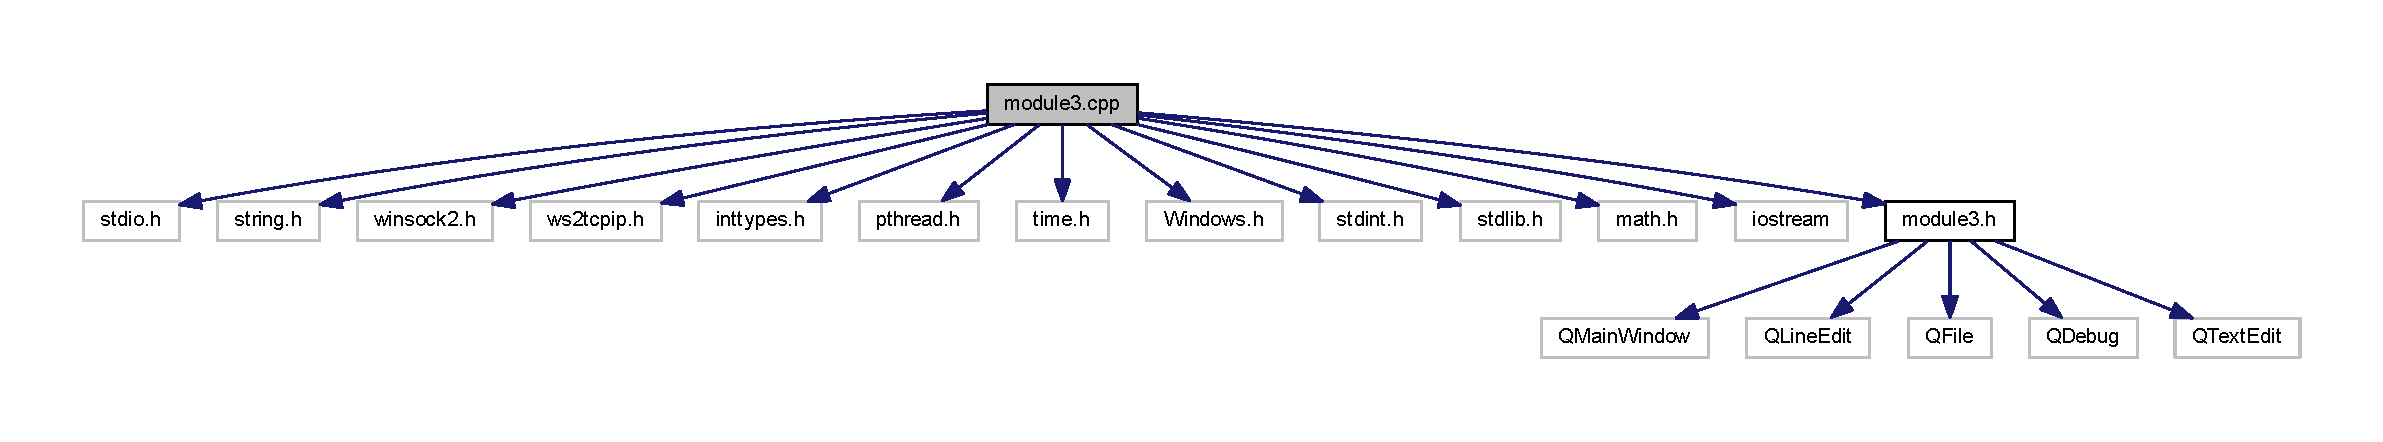
\includegraphics[width=350pt]{module3_8cpp__incl}
\end{center}
\end{figure}
\subsection*{Macros}
\begin{DoxyCompactItemize}
\item 
\#define \mbox{\hyperlink{module3_8cpp_a9bed4a5724ac5d5ff76fbe36f0851323}{H\+A\+V\+E\+\_\+\+S\+T\+R\+U\+C\+T\+\_\+\+T\+I\+M\+E\+S\+P\+EC}}
\end{DoxyCompactItemize}
\subsection*{Functions}
\begin{DoxyCompactItemize}
\item 
void $\ast$ \mbox{\hyperlink{module3_8cpp_a0b1c23a9d0f8a76b936c25c44e739b82}{dequeue\+Loop\+Wrapper}} (void $\ast$arg)
\end{DoxyCompactItemize}
\subsection*{Variables}
\begin{DoxyCompactItemize}
\item 
S\+O\+C\+K\+ET \mbox{\hyperlink{module3_8cpp_ab8fc9c83dd0c6b800727240e351927e9}{s}}
\item 
uint32\+\_\+t \mbox{\hyperlink{module3_8cpp_ab79d0298bf40871324558491e62eeecb}{file\+\_\+cnt}} = 0U
\item 
uint8\+\_\+t \mbox{\hyperlink{module3_8cpp_a4a3da89cf9b53baa4e27e9b8d2a8491d}{done}} = \mbox{\hyperlink{module3_8h_a403d1f0f0fd3c38c0b218c9847d1cd7f}{R\+O\+U\+T\+I\+N\+E\+\_\+\+N\+U\+M\+\_\+\+S\+E\+NT}}
\item 
int \mbox{\hyperlink{module3_8cpp_a1c5675eceda73acf829cc5bd0d171463}{command\+Num}} = -\/1
\item 
uint8\+\_\+t \mbox{\hyperlink{module3_8cpp_a0c0b0e42f272b15d079093e5a73cf71b}{download}} = \mbox{\hyperlink{module3_8h_a5dae31ce3085d355fa86c08fb0b28c7e}{N\+O\+T\+\_\+\+D\+O\+W\+N\+L\+O\+A\+D\+I\+NG}}
\item 
\mbox{\hyperlink{__module3_8h_a58c449f6052675fb4288c20122741cb8}{s\+\_\+\+D\+I\+A\+G\+\_\+\+D\+A\+TA}} \mbox{\hyperlink{module3_8cpp_aefd3928a5dfc916ccd89239ea420907b}{diag\+MsgQ}}
\item 
\mbox{\hyperlink{__module3_8h_a1f542cc6438c66026963a340365d442a}{s\+\_\+\+D\+I\+A\+G\+\_\+\+S\+H\+M\+\_\+\+D\+A\+TA}} \mbox{\hyperlink{module3_8cpp_a242ca4a8d45088539695ad03d2b74116}{diag\+Sh\+Mem}}
\item 
pthread\+\_\+t \mbox{\hyperlink{module3_8cpp_a3a5ba243b3ab4b6093afb178de0f9509}{tid}}
\end{DoxyCompactItemize}


\subsection{Macro Definition Documentation}
\mbox{\Hypertarget{module3_8cpp_a9bed4a5724ac5d5ff76fbe36f0851323}\label{module3_8cpp_a9bed4a5724ac5d5ff76fbe36f0851323}} 
\index{module3.\+cpp@{module3.\+cpp}!H\+A\+V\+E\+\_\+\+S\+T\+R\+U\+C\+T\+\_\+\+T\+I\+M\+E\+S\+P\+EC@{H\+A\+V\+E\+\_\+\+S\+T\+R\+U\+C\+T\+\_\+\+T\+I\+M\+E\+S\+P\+EC}}
\index{H\+A\+V\+E\+\_\+\+S\+T\+R\+U\+C\+T\+\_\+\+T\+I\+M\+E\+S\+P\+EC@{H\+A\+V\+E\+\_\+\+S\+T\+R\+U\+C\+T\+\_\+\+T\+I\+M\+E\+S\+P\+EC}!module3.\+cpp@{module3.\+cpp}}
\subsubsection{\texorpdfstring{H\+A\+V\+E\+\_\+\+S\+T\+R\+U\+C\+T\+\_\+\+T\+I\+M\+E\+S\+P\+EC}{HAVE\_STRUCT\_TIMESPEC}}
{\footnotesize\ttfamily \#define H\+A\+V\+E\+\_\+\+S\+T\+R\+U\+C\+T\+\_\+\+T\+I\+M\+E\+S\+P\+EC}



\subsection{Function Documentation}
\mbox{\Hypertarget{module3_8cpp_a0b1c23a9d0f8a76b936c25c44e739b82}\label{module3_8cpp_a0b1c23a9d0f8a76b936c25c44e739b82}} 
\index{module3.\+cpp@{module3.\+cpp}!dequeue\+Loop\+Wrapper@{dequeue\+Loop\+Wrapper}}
\index{dequeue\+Loop\+Wrapper@{dequeue\+Loop\+Wrapper}!module3.\+cpp@{module3.\+cpp}}
\subsubsection{\texorpdfstring{dequeue\+Loop\+Wrapper()}{dequeueLoopWrapper()}}
{\footnotesize\ttfamily void $\ast$ dequeue\+Loop\+Wrapper (\begin{DoxyParamCaption}\item[{void $\ast$}]{arg }\end{DoxyParamCaption})}

Here is the call graph for this function\+:
\nopagebreak
\begin{figure}[H]
\begin{center}
\leavevmode
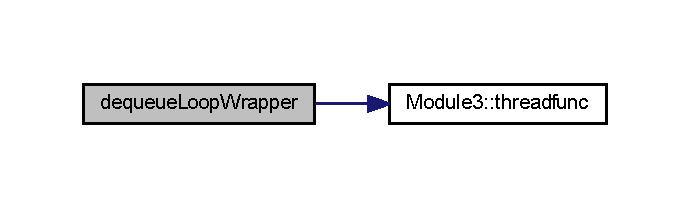
\includegraphics[width=331pt]{module3_8cpp_a0b1c23a9d0f8a76b936c25c44e739b82_cgraph}
\end{center}
\end{figure}


\subsection{Variable Documentation}
\mbox{\Hypertarget{module3_8cpp_a1c5675eceda73acf829cc5bd0d171463}\label{module3_8cpp_a1c5675eceda73acf829cc5bd0d171463}} 
\index{module3.\+cpp@{module3.\+cpp}!command\+Num@{command\+Num}}
\index{command\+Num@{command\+Num}!module3.\+cpp@{module3.\+cpp}}
\subsubsection{\texorpdfstring{command\+Num}{commandNum}}
{\footnotesize\ttfamily int command\+Num = -\/1}

\mbox{\Hypertarget{module3_8cpp_aefd3928a5dfc916ccd89239ea420907b}\label{module3_8cpp_aefd3928a5dfc916ccd89239ea420907b}} 
\index{module3.\+cpp@{module3.\+cpp}!diag\+MsgQ@{diag\+MsgQ}}
\index{diag\+MsgQ@{diag\+MsgQ}!module3.\+cpp@{module3.\+cpp}}
\subsubsection{\texorpdfstring{diag\+MsgQ}{diagMsgQ}}
{\footnotesize\ttfamily \mbox{\hyperlink{__module3_8h_a58c449f6052675fb4288c20122741cb8}{s\+\_\+\+D\+I\+A\+G\+\_\+\+D\+A\+TA}} diag\+MsgQ}

\mbox{\Hypertarget{module3_8cpp_a242ca4a8d45088539695ad03d2b74116}\label{module3_8cpp_a242ca4a8d45088539695ad03d2b74116}} 
\index{module3.\+cpp@{module3.\+cpp}!diag\+Sh\+Mem@{diag\+Sh\+Mem}}
\index{diag\+Sh\+Mem@{diag\+Sh\+Mem}!module3.\+cpp@{module3.\+cpp}}
\subsubsection{\texorpdfstring{diag\+Sh\+Mem}{diagShMem}}
{\footnotesize\ttfamily \mbox{\hyperlink{__module3_8h_a1f542cc6438c66026963a340365d442a}{s\+\_\+\+D\+I\+A\+G\+\_\+\+S\+H\+M\+\_\+\+D\+A\+TA}} diag\+Sh\+Mem}

\mbox{\Hypertarget{module3_8cpp_a4a3da89cf9b53baa4e27e9b8d2a8491d}\label{module3_8cpp_a4a3da89cf9b53baa4e27e9b8d2a8491d}} 
\index{module3.\+cpp@{module3.\+cpp}!done@{done}}
\index{done@{done}!module3.\+cpp@{module3.\+cpp}}
\subsubsection{\texorpdfstring{done}{done}}
{\footnotesize\ttfamily uint8\+\_\+t done = \mbox{\hyperlink{module3_8h_a403d1f0f0fd3c38c0b218c9847d1cd7f}{R\+O\+U\+T\+I\+N\+E\+\_\+\+N\+U\+M\+\_\+\+S\+E\+NT}}}

\mbox{\Hypertarget{module3_8cpp_a0c0b0e42f272b15d079093e5a73cf71b}\label{module3_8cpp_a0c0b0e42f272b15d079093e5a73cf71b}} 
\index{module3.\+cpp@{module3.\+cpp}!download@{download}}
\index{download@{download}!module3.\+cpp@{module3.\+cpp}}
\subsubsection{\texorpdfstring{download}{download}}
{\footnotesize\ttfamily uint8\+\_\+t download = \mbox{\hyperlink{module3_8h_a5dae31ce3085d355fa86c08fb0b28c7e}{N\+O\+T\+\_\+\+D\+O\+W\+N\+L\+O\+A\+D\+I\+NG}}}

\mbox{\Hypertarget{module3_8cpp_ab79d0298bf40871324558491e62eeecb}\label{module3_8cpp_ab79d0298bf40871324558491e62eeecb}} 
\index{module3.\+cpp@{module3.\+cpp}!file\+\_\+cnt@{file\+\_\+cnt}}
\index{file\+\_\+cnt@{file\+\_\+cnt}!module3.\+cpp@{module3.\+cpp}}
\subsubsection{\texorpdfstring{file\+\_\+cnt}{file\_cnt}}
{\footnotesize\ttfamily uint32\+\_\+t file\+\_\+cnt = 0U}

\mbox{\Hypertarget{module3_8cpp_ab8fc9c83dd0c6b800727240e351927e9}\label{module3_8cpp_ab8fc9c83dd0c6b800727240e351927e9}} 
\index{module3.\+cpp@{module3.\+cpp}!s@{s}}
\index{s@{s}!module3.\+cpp@{module3.\+cpp}}
\subsubsection{\texorpdfstring{s}{s}}
{\footnotesize\ttfamily S\+O\+C\+K\+ET s}

\mbox{\Hypertarget{module3_8cpp_a3a5ba243b3ab4b6093afb178de0f9509}\label{module3_8cpp_a3a5ba243b3ab4b6093afb178de0f9509}} 
\index{module3.\+cpp@{module3.\+cpp}!tid@{tid}}
\index{tid@{tid}!module3.\+cpp@{module3.\+cpp}}
\subsubsection{\texorpdfstring{tid}{tid}}
{\footnotesize\ttfamily pthread\+\_\+t tid}


\hypertarget{module3_8h}{}\section{module3.\+h File Reference}
\label{module3_8h}\index{module3.\+h@{module3.\+h}}
{\ttfamily \#include $<$Q\+Main\+Window$>$}\newline
{\ttfamily \#include $<$Q\+Line\+Edit$>$}\newline
{\ttfamily \#include $<$Q\+File$>$}\newline
{\ttfamily \#include $<$Q\+Debug$>$}\newline
{\ttfamily \#include $<$Q\+Text\+Edit$>$}\newline
Include dependency graph for module3.\+h\+:
\nopagebreak
\begin{figure}[H]
\begin{center}
\leavevmode
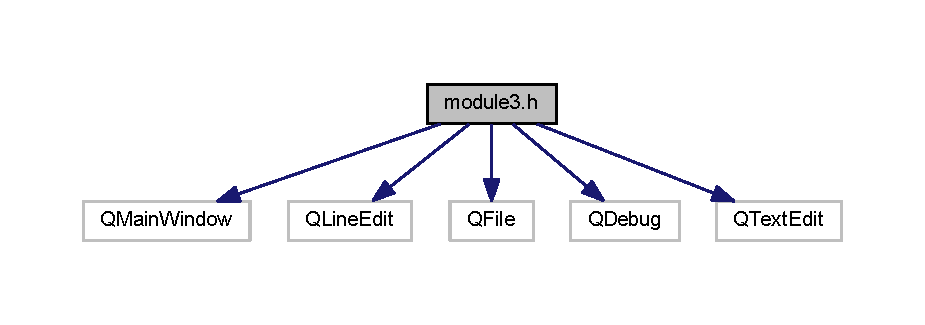
\includegraphics[width=350pt]{module3_8h__incl}
\end{center}
\end{figure}
This graph shows which files directly or indirectly include this file\+:
\nopagebreak
\begin{figure}[H]
\begin{center}
\leavevmode
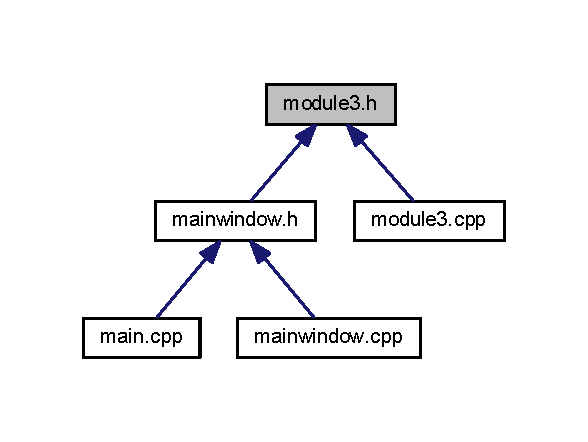
\includegraphics[width=282pt]{module3_8h__dep__incl}
\end{center}
\end{figure}
\subsection*{Classes}
\begin{DoxyCompactItemize}
\item 
struct \mbox{\hyperlink{structerror_struct}{error\+Struct}}
\item 
struct \mbox{\hyperlink{structdiagnostic_data_msg_q}{diagnostic\+Data\+MsgQ}}
\item 
struct \mbox{\hyperlink{structdiagnostic_data_sh_m}{diagnostic\+Data\+ShM}}
\item 
class \mbox{\hyperlink{class_module3}{Module3}}
\end{DoxyCompactItemize}
\subsection*{Namespaces}
\begin{DoxyCompactItemize}
\item 
 \mbox{\hyperlink{namespace_ui}{Ui}}
\end{DoxyCompactItemize}
\subsection*{Macros}
\begin{DoxyCompactItemize}
\item 
\#define \mbox{\hyperlink{module3_8h_adfc8f90f3a8caa8423099cf36ff214f1}{\+\_\+\+W\+I\+N\+S\+O\+C\+K\+\_\+\+D\+E\+P\+R\+E\+C\+A\+T\+E\+D\+\_\+\+N\+O\+\_\+\+W\+A\+R\+N\+I\+N\+GS}}
\item 
\#define \mbox{\hyperlink{module3_8h_abe0b7b2a0ec4b64b92585808a051e1fa}{S\+L\+E\+E\+P\+\_\+\+T\+I\+ME}}~15
\item 
\#define \mbox{\hyperlink{module3_8h_afd8807aef011a7518ea028a4d29ebd4a}{S\+W\+U\+\_\+\+B\+R\+\_\+\+S\+E\+R\+V\+E\+R\+P\+O\+RT}}~29170
\item 
\#define \mbox{\hyperlink{module3_8h_ab3570d75ac730a357320f9d5dae2c884}{S\+W\+U\+\_\+\+B\+R\+\_\+\+C\+L\+I\+E\+N\+T\+P\+O\+RT}}~29171
\item 
\#define \mbox{\hyperlink{module3_8h_ad974fe981249f5e84fbf1683b012c9f8}{B\+U\+F\+L\+EN}}~512
\item 
\#define \mbox{\hyperlink{module3_8h_aca9322dca2cb4e10ba445ecf867885c1}{z\+F\+A\+S\+\_\+\+I\+Pv4}}~\char`\"{}192.\+168.\+122.\+60\char`\"{}
\item 
\#define \mbox{\hyperlink{module3_8h_a403d1f0f0fd3c38c0b218c9847d1cd7f}{R\+O\+U\+T\+I\+N\+E\+\_\+\+N\+U\+M\+\_\+\+S\+E\+NT}}~1
\item 
\#define \mbox{\hyperlink{module3_8h_aea79debee44db16ecd24760ee03cb84c}{R\+O\+U\+T\+I\+N\+E\+\_\+\+N\+U\+M\+\_\+\+N\+O\+T\+\_\+\+S\+E\+NT}}~0
\item 
\#define \mbox{\hyperlink{module3_8h_a84a7e33e8efc6438973bc1cf89839cbe}{D\+O\+W\+N\+L\+O\+A\+D\+\_\+\+I\+N\+\_\+\+P\+R\+O\+G\+R\+E\+SS}}~1
\item 
\#define \mbox{\hyperlink{module3_8h_a5dae31ce3085d355fa86c08fb0b28c7e}{N\+O\+T\+\_\+\+D\+O\+W\+N\+L\+O\+A\+D\+I\+NG}}~0
\item 
\#define \mbox{\hyperlink{module3_8h_a45cd8099107d7234da997c1d83f6f7f0}{T\+E\+R\+M\+I\+N\+A\+T\+E\+\_\+\+P\+R\+O\+G\+R\+AM}}~0
\item 
\#define \mbox{\hyperlink{module3_8h_ad797720c6e0fe8ffae0c44788a3be2c9}{D\+O\+W\+N\+L\+O\+A\+D\+\_\+\+F\+I\+LE}}~1
\item 
\#define \mbox{\hyperlink{module3_8h_a4436650e34eccca9dcd7f12c76317dba}{G\+E\+T\+\_\+\+M\+S\+GQ}}~3
\item 
\#define \mbox{\hyperlink{module3_8h_a7915ff1cb0778b5491fd2e55f9ad46e1}{G\+E\+T\+\_\+\+S\+H\+M\+EM}}~4
\end{DoxyCompactItemize}
\subsection*{Typedefs}
\begin{DoxyCompactItemize}
\item 
typedef struct \mbox{\hyperlink{structerror_struct}{error\+Struct}} \mbox{\hyperlink{module3_8h_aed782b3a5727361a6b656be14d539f9c}{s\+\_\+\+E\+R\+R\+O\+RS}}
\item 
typedef struct \mbox{\hyperlink{structdiagnostic_data_msg_q}{diagnostic\+Data\+MsgQ}} \mbox{\hyperlink{module3_8h_a58c449f6052675fb4288c20122741cb8}{s\+\_\+\+D\+I\+A\+G\+\_\+\+D\+A\+TA}}
\item 
typedef struct \mbox{\hyperlink{structdiagnostic_data_sh_m}{diagnostic\+Data\+ShM}} \mbox{\hyperlink{module3_8h_a1f542cc6438c66026963a340365d442a}{s\+\_\+\+D\+I\+A\+G\+\_\+\+S\+H\+M\+\_\+\+D\+A\+TA}}
\end{DoxyCompactItemize}


\subsection{Macro Definition Documentation}
\mbox{\Hypertarget{module3_8h_adfc8f90f3a8caa8423099cf36ff214f1}\label{module3_8h_adfc8f90f3a8caa8423099cf36ff214f1}} 
\index{module3.\+h@{module3.\+h}!\+\_\+\+W\+I\+N\+S\+O\+C\+K\+\_\+\+D\+E\+P\+R\+E\+C\+A\+T\+E\+D\+\_\+\+N\+O\+\_\+\+W\+A\+R\+N\+I\+N\+GS@{\+\_\+\+W\+I\+N\+S\+O\+C\+K\+\_\+\+D\+E\+P\+R\+E\+C\+A\+T\+E\+D\+\_\+\+N\+O\+\_\+\+W\+A\+R\+N\+I\+N\+GS}}
\index{\+\_\+\+W\+I\+N\+S\+O\+C\+K\+\_\+\+D\+E\+P\+R\+E\+C\+A\+T\+E\+D\+\_\+\+N\+O\+\_\+\+W\+A\+R\+N\+I\+N\+GS@{\+\_\+\+W\+I\+N\+S\+O\+C\+K\+\_\+\+D\+E\+P\+R\+E\+C\+A\+T\+E\+D\+\_\+\+N\+O\+\_\+\+W\+A\+R\+N\+I\+N\+GS}!module3.\+h@{module3.\+h}}
\subsubsection{\texorpdfstring{\+\_\+\+W\+I\+N\+S\+O\+C\+K\+\_\+\+D\+E\+P\+R\+E\+C\+A\+T\+E\+D\+\_\+\+N\+O\+\_\+\+W\+A\+R\+N\+I\+N\+GS}{\_WINSOCK\_DEPRECATED\_NO\_WARNINGS}}
{\footnotesize\ttfamily \#define \+\_\+\+W\+I\+N\+S\+O\+C\+K\+\_\+\+D\+E\+P\+R\+E\+C\+A\+T\+E\+D\+\_\+\+N\+O\+\_\+\+W\+A\+R\+N\+I\+N\+GS}

\mbox{\Hypertarget{module3_8h_ad974fe981249f5e84fbf1683b012c9f8}\label{module3_8h_ad974fe981249f5e84fbf1683b012c9f8}} 
\index{module3.\+h@{module3.\+h}!B\+U\+F\+L\+EN@{B\+U\+F\+L\+EN}}
\index{B\+U\+F\+L\+EN@{B\+U\+F\+L\+EN}!module3.\+h@{module3.\+h}}
\subsubsection{\texorpdfstring{B\+U\+F\+L\+EN}{BUFLEN}}
{\footnotesize\ttfamily \#define B\+U\+F\+L\+EN~512}

\mbox{\Hypertarget{module3_8h_ad797720c6e0fe8ffae0c44788a3be2c9}\label{module3_8h_ad797720c6e0fe8ffae0c44788a3be2c9}} 
\index{module3.\+h@{module3.\+h}!D\+O\+W\+N\+L\+O\+A\+D\+\_\+\+F\+I\+LE@{D\+O\+W\+N\+L\+O\+A\+D\+\_\+\+F\+I\+LE}}
\index{D\+O\+W\+N\+L\+O\+A\+D\+\_\+\+F\+I\+LE@{D\+O\+W\+N\+L\+O\+A\+D\+\_\+\+F\+I\+LE}!module3.\+h@{module3.\+h}}
\subsubsection{\texorpdfstring{D\+O\+W\+N\+L\+O\+A\+D\+\_\+\+F\+I\+LE}{DOWNLOAD\_FILE}}
{\footnotesize\ttfamily \#define D\+O\+W\+N\+L\+O\+A\+D\+\_\+\+F\+I\+LE~1}

\mbox{\Hypertarget{module3_8h_a84a7e33e8efc6438973bc1cf89839cbe}\label{module3_8h_a84a7e33e8efc6438973bc1cf89839cbe}} 
\index{module3.\+h@{module3.\+h}!D\+O\+W\+N\+L\+O\+A\+D\+\_\+\+I\+N\+\_\+\+P\+R\+O\+G\+R\+E\+SS@{D\+O\+W\+N\+L\+O\+A\+D\+\_\+\+I\+N\+\_\+\+P\+R\+O\+G\+R\+E\+SS}}
\index{D\+O\+W\+N\+L\+O\+A\+D\+\_\+\+I\+N\+\_\+\+P\+R\+O\+G\+R\+E\+SS@{D\+O\+W\+N\+L\+O\+A\+D\+\_\+\+I\+N\+\_\+\+P\+R\+O\+G\+R\+E\+SS}!module3.\+h@{module3.\+h}}
\subsubsection{\texorpdfstring{D\+O\+W\+N\+L\+O\+A\+D\+\_\+\+I\+N\+\_\+\+P\+R\+O\+G\+R\+E\+SS}{DOWNLOAD\_IN\_PROGRESS}}
{\footnotesize\ttfamily \#define D\+O\+W\+N\+L\+O\+A\+D\+\_\+\+I\+N\+\_\+\+P\+R\+O\+G\+R\+E\+SS~1}

\mbox{\Hypertarget{module3_8h_a4436650e34eccca9dcd7f12c76317dba}\label{module3_8h_a4436650e34eccca9dcd7f12c76317dba}} 
\index{module3.\+h@{module3.\+h}!G\+E\+T\+\_\+\+M\+S\+GQ@{G\+E\+T\+\_\+\+M\+S\+GQ}}
\index{G\+E\+T\+\_\+\+M\+S\+GQ@{G\+E\+T\+\_\+\+M\+S\+GQ}!module3.\+h@{module3.\+h}}
\subsubsection{\texorpdfstring{G\+E\+T\+\_\+\+M\+S\+GQ}{GET\_MSGQ}}
{\footnotesize\ttfamily \#define G\+E\+T\+\_\+\+M\+S\+GQ~3}

\mbox{\Hypertarget{module3_8h_a7915ff1cb0778b5491fd2e55f9ad46e1}\label{module3_8h_a7915ff1cb0778b5491fd2e55f9ad46e1}} 
\index{module3.\+h@{module3.\+h}!G\+E\+T\+\_\+\+S\+H\+M\+EM@{G\+E\+T\+\_\+\+S\+H\+M\+EM}}
\index{G\+E\+T\+\_\+\+S\+H\+M\+EM@{G\+E\+T\+\_\+\+S\+H\+M\+EM}!module3.\+h@{module3.\+h}}
\subsubsection{\texorpdfstring{G\+E\+T\+\_\+\+S\+H\+M\+EM}{GET\_SHMEM}}
{\footnotesize\ttfamily \#define G\+E\+T\+\_\+\+S\+H\+M\+EM~4}

\mbox{\Hypertarget{module3_8h_a5dae31ce3085d355fa86c08fb0b28c7e}\label{module3_8h_a5dae31ce3085d355fa86c08fb0b28c7e}} 
\index{module3.\+h@{module3.\+h}!N\+O\+T\+\_\+\+D\+O\+W\+N\+L\+O\+A\+D\+I\+NG@{N\+O\+T\+\_\+\+D\+O\+W\+N\+L\+O\+A\+D\+I\+NG}}
\index{N\+O\+T\+\_\+\+D\+O\+W\+N\+L\+O\+A\+D\+I\+NG@{N\+O\+T\+\_\+\+D\+O\+W\+N\+L\+O\+A\+D\+I\+NG}!module3.\+h@{module3.\+h}}
\subsubsection{\texorpdfstring{N\+O\+T\+\_\+\+D\+O\+W\+N\+L\+O\+A\+D\+I\+NG}{NOT\_DOWNLOADING}}
{\footnotesize\ttfamily \#define N\+O\+T\+\_\+\+D\+O\+W\+N\+L\+O\+A\+D\+I\+NG~0}

\mbox{\Hypertarget{module3_8h_aea79debee44db16ecd24760ee03cb84c}\label{module3_8h_aea79debee44db16ecd24760ee03cb84c}} 
\index{module3.\+h@{module3.\+h}!R\+O\+U\+T\+I\+N\+E\+\_\+\+N\+U\+M\+\_\+\+N\+O\+T\+\_\+\+S\+E\+NT@{R\+O\+U\+T\+I\+N\+E\+\_\+\+N\+U\+M\+\_\+\+N\+O\+T\+\_\+\+S\+E\+NT}}
\index{R\+O\+U\+T\+I\+N\+E\+\_\+\+N\+U\+M\+\_\+\+N\+O\+T\+\_\+\+S\+E\+NT@{R\+O\+U\+T\+I\+N\+E\+\_\+\+N\+U\+M\+\_\+\+N\+O\+T\+\_\+\+S\+E\+NT}!module3.\+h@{module3.\+h}}
\subsubsection{\texorpdfstring{R\+O\+U\+T\+I\+N\+E\+\_\+\+N\+U\+M\+\_\+\+N\+O\+T\+\_\+\+S\+E\+NT}{ROUTINE\_NUM\_NOT\_SENT}}
{\footnotesize\ttfamily \#define R\+O\+U\+T\+I\+N\+E\+\_\+\+N\+U\+M\+\_\+\+N\+O\+T\+\_\+\+S\+E\+NT~0}

\mbox{\Hypertarget{module3_8h_a403d1f0f0fd3c38c0b218c9847d1cd7f}\label{module3_8h_a403d1f0f0fd3c38c0b218c9847d1cd7f}} 
\index{module3.\+h@{module3.\+h}!R\+O\+U\+T\+I\+N\+E\+\_\+\+N\+U\+M\+\_\+\+S\+E\+NT@{R\+O\+U\+T\+I\+N\+E\+\_\+\+N\+U\+M\+\_\+\+S\+E\+NT}}
\index{R\+O\+U\+T\+I\+N\+E\+\_\+\+N\+U\+M\+\_\+\+S\+E\+NT@{R\+O\+U\+T\+I\+N\+E\+\_\+\+N\+U\+M\+\_\+\+S\+E\+NT}!module3.\+h@{module3.\+h}}
\subsubsection{\texorpdfstring{R\+O\+U\+T\+I\+N\+E\+\_\+\+N\+U\+M\+\_\+\+S\+E\+NT}{ROUTINE\_NUM\_SENT}}
{\footnotesize\ttfamily \#define R\+O\+U\+T\+I\+N\+E\+\_\+\+N\+U\+M\+\_\+\+S\+E\+NT~1}

\mbox{\Hypertarget{module3_8h_abe0b7b2a0ec4b64b92585808a051e1fa}\label{module3_8h_abe0b7b2a0ec4b64b92585808a051e1fa}} 
\index{module3.\+h@{module3.\+h}!S\+L\+E\+E\+P\+\_\+\+T\+I\+ME@{S\+L\+E\+E\+P\+\_\+\+T\+I\+ME}}
\index{S\+L\+E\+E\+P\+\_\+\+T\+I\+ME@{S\+L\+E\+E\+P\+\_\+\+T\+I\+ME}!module3.\+h@{module3.\+h}}
\subsubsection{\texorpdfstring{S\+L\+E\+E\+P\+\_\+\+T\+I\+ME}{SLEEP\_TIME}}
{\footnotesize\ttfamily \#define S\+L\+E\+E\+P\+\_\+\+T\+I\+ME~15}

\mbox{\Hypertarget{module3_8h_ab3570d75ac730a357320f9d5dae2c884}\label{module3_8h_ab3570d75ac730a357320f9d5dae2c884}} 
\index{module3.\+h@{module3.\+h}!S\+W\+U\+\_\+\+B\+R\+\_\+\+C\+L\+I\+E\+N\+T\+P\+O\+RT@{S\+W\+U\+\_\+\+B\+R\+\_\+\+C\+L\+I\+E\+N\+T\+P\+O\+RT}}
\index{S\+W\+U\+\_\+\+B\+R\+\_\+\+C\+L\+I\+E\+N\+T\+P\+O\+RT@{S\+W\+U\+\_\+\+B\+R\+\_\+\+C\+L\+I\+E\+N\+T\+P\+O\+RT}!module3.\+h@{module3.\+h}}
\subsubsection{\texorpdfstring{S\+W\+U\+\_\+\+B\+R\+\_\+\+C\+L\+I\+E\+N\+T\+P\+O\+RT}{SWU\_BR\_CLIENTPORT}}
{\footnotesize\ttfamily \#define S\+W\+U\+\_\+\+B\+R\+\_\+\+C\+L\+I\+E\+N\+T\+P\+O\+RT~29171}

\mbox{\Hypertarget{module3_8h_afd8807aef011a7518ea028a4d29ebd4a}\label{module3_8h_afd8807aef011a7518ea028a4d29ebd4a}} 
\index{module3.\+h@{module3.\+h}!S\+W\+U\+\_\+\+B\+R\+\_\+\+S\+E\+R\+V\+E\+R\+P\+O\+RT@{S\+W\+U\+\_\+\+B\+R\+\_\+\+S\+E\+R\+V\+E\+R\+P\+O\+RT}}
\index{S\+W\+U\+\_\+\+B\+R\+\_\+\+S\+E\+R\+V\+E\+R\+P\+O\+RT@{S\+W\+U\+\_\+\+B\+R\+\_\+\+S\+E\+R\+V\+E\+R\+P\+O\+RT}!module3.\+h@{module3.\+h}}
\subsubsection{\texorpdfstring{S\+W\+U\+\_\+\+B\+R\+\_\+\+S\+E\+R\+V\+E\+R\+P\+O\+RT}{SWU\_BR\_SERVERPORT}}
{\footnotesize\ttfamily \#define S\+W\+U\+\_\+\+B\+R\+\_\+\+S\+E\+R\+V\+E\+R\+P\+O\+RT~29170}

\mbox{\Hypertarget{module3_8h_a45cd8099107d7234da997c1d83f6f7f0}\label{module3_8h_a45cd8099107d7234da997c1d83f6f7f0}} 
\index{module3.\+h@{module3.\+h}!T\+E\+R\+M\+I\+N\+A\+T\+E\+\_\+\+P\+R\+O\+G\+R\+AM@{T\+E\+R\+M\+I\+N\+A\+T\+E\+\_\+\+P\+R\+O\+G\+R\+AM}}
\index{T\+E\+R\+M\+I\+N\+A\+T\+E\+\_\+\+P\+R\+O\+G\+R\+AM@{T\+E\+R\+M\+I\+N\+A\+T\+E\+\_\+\+P\+R\+O\+G\+R\+AM}!module3.\+h@{module3.\+h}}
\subsubsection{\texorpdfstring{T\+E\+R\+M\+I\+N\+A\+T\+E\+\_\+\+P\+R\+O\+G\+R\+AM}{TERMINATE\_PROGRAM}}
{\footnotesize\ttfamily \#define T\+E\+R\+M\+I\+N\+A\+T\+E\+\_\+\+P\+R\+O\+G\+R\+AM~0}

\mbox{\Hypertarget{module3_8h_aca9322dca2cb4e10ba445ecf867885c1}\label{module3_8h_aca9322dca2cb4e10ba445ecf867885c1}} 
\index{module3.\+h@{module3.\+h}!z\+F\+A\+S\+\_\+\+I\+Pv4@{z\+F\+A\+S\+\_\+\+I\+Pv4}}
\index{z\+F\+A\+S\+\_\+\+I\+Pv4@{z\+F\+A\+S\+\_\+\+I\+Pv4}!module3.\+h@{module3.\+h}}
\subsubsection{\texorpdfstring{z\+F\+A\+S\+\_\+\+I\+Pv4}{zFAS\_IPv4}}
{\footnotesize\ttfamily \#define z\+F\+A\+S\+\_\+\+I\+Pv4~\char`\"{}192.\+168.\+122.\+60\char`\"{}}



\subsection{Typedef Documentation}
\mbox{\Hypertarget{module3_8h_a58c449f6052675fb4288c20122741cb8}\label{module3_8h_a58c449f6052675fb4288c20122741cb8}} 
\index{module3.\+h@{module3.\+h}!s\+\_\+\+D\+I\+A\+G\+\_\+\+D\+A\+TA@{s\+\_\+\+D\+I\+A\+G\+\_\+\+D\+A\+TA}}
\index{s\+\_\+\+D\+I\+A\+G\+\_\+\+D\+A\+TA@{s\+\_\+\+D\+I\+A\+G\+\_\+\+D\+A\+TA}!module3.\+h@{module3.\+h}}
\subsubsection{\texorpdfstring{s\+\_\+\+D\+I\+A\+G\+\_\+\+D\+A\+TA}{s\_DIAG\_DATA}}
{\footnotesize\ttfamily typedef struct \mbox{\hyperlink{structdiagnostic_data_msg_q}{diagnostic\+Data\+MsgQ}}  \mbox{\hyperlink{__module3_8h_a58c449f6052675fb4288c20122741cb8}{s\+\_\+\+D\+I\+A\+G\+\_\+\+D\+A\+TA}}}

\mbox{\Hypertarget{module3_8h_a1f542cc6438c66026963a340365d442a}\label{module3_8h_a1f542cc6438c66026963a340365d442a}} 
\index{module3.\+h@{module3.\+h}!s\+\_\+\+D\+I\+A\+G\+\_\+\+S\+H\+M\+\_\+\+D\+A\+TA@{s\+\_\+\+D\+I\+A\+G\+\_\+\+S\+H\+M\+\_\+\+D\+A\+TA}}
\index{s\+\_\+\+D\+I\+A\+G\+\_\+\+S\+H\+M\+\_\+\+D\+A\+TA@{s\+\_\+\+D\+I\+A\+G\+\_\+\+S\+H\+M\+\_\+\+D\+A\+TA}!module3.\+h@{module3.\+h}}
\subsubsection{\texorpdfstring{s\+\_\+\+D\+I\+A\+G\+\_\+\+S\+H\+M\+\_\+\+D\+A\+TA}{s\_DIAG\_SHM\_DATA}}
{\footnotesize\ttfamily typedef struct \mbox{\hyperlink{structdiagnostic_data_sh_m}{diagnostic\+Data\+ShM}}  \mbox{\hyperlink{__module3_8h_a1f542cc6438c66026963a340365d442a}{s\+\_\+\+D\+I\+A\+G\+\_\+\+S\+H\+M\+\_\+\+D\+A\+TA}}}

\mbox{\Hypertarget{module3_8h_aed782b3a5727361a6b656be14d539f9c}\label{module3_8h_aed782b3a5727361a6b656be14d539f9c}} 
\index{module3.\+h@{module3.\+h}!s\+\_\+\+E\+R\+R\+O\+RS@{s\+\_\+\+E\+R\+R\+O\+RS}}
\index{s\+\_\+\+E\+R\+R\+O\+RS@{s\+\_\+\+E\+R\+R\+O\+RS}!module3.\+h@{module3.\+h}}
\subsubsection{\texorpdfstring{s\+\_\+\+E\+R\+R\+O\+RS}{s\_ERRORS}}
{\footnotesize\ttfamily typedef struct \mbox{\hyperlink{structerror_struct}{error\+Struct}} \mbox{\hyperlink{__module3_8h_aed782b3a5727361a6b656be14d539f9c}{s\+\_\+\+E\+R\+R\+O\+RS}}}


\hypertarget{module_one_handle_routines_8c}{}\section{module\+One\+Handle\+Routines.\+c File Reference}
\label{module_one_handle_routines_8c}\index{module\+One\+Handle\+Routines.\+c@{module\+One\+Handle\+Routines.\+c}}


Functions for receiving routine numbers and starting test modes.  


{\ttfamily \#include $<$vxworks.\+h$>$}\newline
{\ttfamily \#include $<$stdio.\+h$>$}\newline
{\ttfamily \#include $<$unistd.\+h$>$}\newline
{\ttfamily \#include $<$ping6\+Lib.\+h$>$}\newline
{\ttfamily \#include $<$msg\+Q\+Lib\+Common.\+h$>$}\newline
{\ttfamily \#include $<$task\+Lib\+Common.\+h$>$}\newline
{\ttfamily \#include \char`\"{}module\+One\+Read\+Eth\+Phy.\+h\char`\"{}}\newline
{\ttfamily \#include \char`\"{}module\+One\+Handle\+Routines.\+h\char`\"{}}\newline
Include dependency graph for module\+One\+Handle\+Routines.\+c\+:
\nopagebreak
\begin{figure}[H]
\begin{center}
\leavevmode
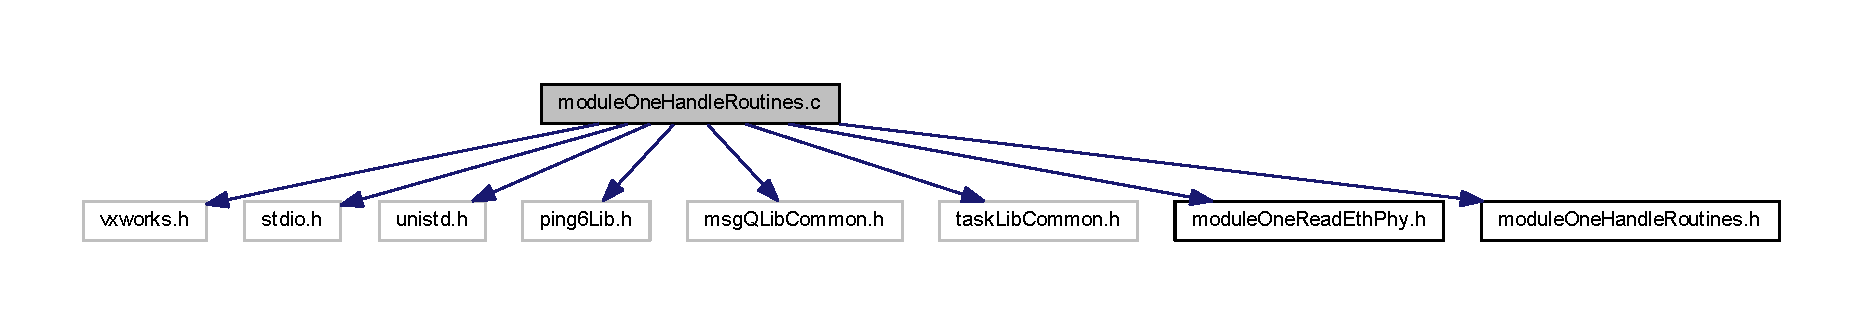
\includegraphics[width=350pt]{module_one_handle_routines_8c__incl}
\end{center}
\end{figure}
\subsection*{Functions}
\begin{DoxyCompactItemize}
\item 
L\+O\+C\+AL void \mbox{\hyperlink{module_one_handle_routines_8c_a13ffca776e207f720598fece14e32d41}{\+\_\+test\+Modes}} (int routine\+\_\+trigger)
\begin{DoxyCompactList}\small\item\em This function is used for activating test routines. \end{DoxyCompactList}\item 
L\+O\+C\+AL S\+T\+A\+T\+US \mbox{\hyperlink{module_one_handle_routines_8c_ace50ff396b856ee978590de17c77ad4f}{\+\_\+ping\+Routine}} (void)
\begin{DoxyCompactList}\small\item\em Routine used to ping PC when triggered. \end{DoxyCompactList}\item 
L\+O\+C\+AL void \mbox{\hyperlink{module_one_handle_routines_8c_a282d3cba04d9f8a400fbf53f683cbb7c}{\+\_\+normal\+Operation\+Test}} (uint16\+\_\+t mode)
\begin{DoxyCompactList}\small\item\em Routine for testing normal operation mode. \end{DoxyCompactList}\item 
void \mbox{\hyperlink{module_one_handle_routines_8c_a9d76ff69513e544453fdcbcb8fc5184c}{module1\+\_\+\+Get\+Routine\+Num}} (void)
\begin{DoxyCompactList}\small\item\em This function gets number of routine which will be called and calls \mbox{\hyperlink{module_one_handle_routines_8c_a13ffca776e207f720598fece14e32d41}{\+\_\+test\+Modes(int routine\+\_\+trigger)}}. \end{DoxyCompactList}\end{DoxyCompactItemize}


\subsection{Detailed Description}
Functions for receiving routine numbers and starting test modes. 

\mbox{\hyperlink{module_one_handle_routines_8c}{module\+One\+Handle\+Routines.\+c}}

\begin{DoxyVersion}{Version}
\mbox{[}7-\/\+Jun-\/2018\mbox{]} \mbox{[}Stefan Masalusic\mbox{]} Initial creation  \mbox{[}7-\/\+May-\/2018\mbox{]} Added module1\+\_\+\+Get\+Routine\+Num function \mbox{[}9-\/\+May-\/2018\mbox{]} Added \+\_\+test\+Modes, \+\_\+ping\+Routine and \+\_\+normal\+Operation\+Test functions ~\newline
\subsubsection*{\mbox{[}24-\/\+May-\/2018\mbox{]} Added function descriptions }
\end{DoxyVersion}


\subsection{Function Documentation}
\mbox{\Hypertarget{module_one_handle_routines_8c_a282d3cba04d9f8a400fbf53f683cbb7c}\label{module_one_handle_routines_8c_a282d3cba04d9f8a400fbf53f683cbb7c}} 
\index{module\+One\+Handle\+Routines.\+c@{module\+One\+Handle\+Routines.\+c}!\+\_\+normal\+Operation\+Test@{\+\_\+normal\+Operation\+Test}}
\index{\+\_\+normal\+Operation\+Test@{\+\_\+normal\+Operation\+Test}!module\+One\+Handle\+Routines.\+c@{module\+One\+Handle\+Routines.\+c}}
\subsubsection{\texorpdfstring{\+\_\+normal\+Operation\+Test()}{\_normalOperationTest()}}
{\footnotesize\ttfamily L\+O\+C\+AL void \+\_\+normal\+Operation\+Test (\begin{DoxyParamCaption}\item[{uint16\+\_\+t}]{mode }\end{DoxyParamCaption})}



Routine for testing normal operation mode. 


\begin{DoxyParams}{Parameters}
{\em mode} & Number of routine mode \\
\hline
\end{DoxyParams}
Here is the call graph for this function\+:
\nopagebreak
\begin{figure}[H]
\begin{center}
\leavevmode
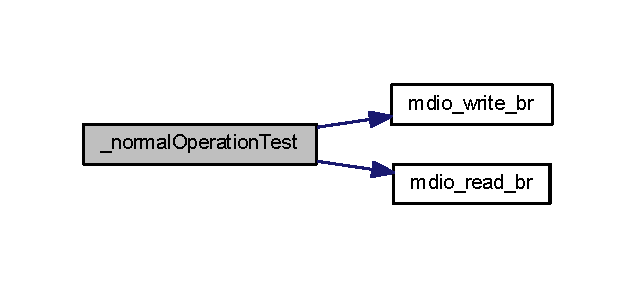
\includegraphics[width=305pt]{module_one_handle_routines_8c_a282d3cba04d9f8a400fbf53f683cbb7c_cgraph}
\end{center}
\end{figure}
\mbox{\Hypertarget{module_one_handle_routines_8c_ace50ff396b856ee978590de17c77ad4f}\label{module_one_handle_routines_8c_ace50ff396b856ee978590de17c77ad4f}} 
\index{module\+One\+Handle\+Routines.\+c@{module\+One\+Handle\+Routines.\+c}!\+\_\+ping\+Routine@{\+\_\+ping\+Routine}}
\index{\+\_\+ping\+Routine@{\+\_\+ping\+Routine}!module\+One\+Handle\+Routines.\+c@{module\+One\+Handle\+Routines.\+c}}
\subsubsection{\texorpdfstring{\+\_\+ping\+Routine()}{\_pingRoutine()}}
{\footnotesize\ttfamily L\+O\+C\+AL S\+T\+A\+T\+US \+\_\+ping\+Routine (\begin{DoxyParamCaption}\item[{void}]{ }\end{DoxyParamCaption})}



Routine used to ping PC when triggered. 

\begin{DoxyReturn}{Returns}
OK if successful, E\+R\+R\+OR otherwise 
\end{DoxyReturn}
\mbox{\Hypertarget{module_one_handle_routines_8c_a13ffca776e207f720598fece14e32d41}\label{module_one_handle_routines_8c_a13ffca776e207f720598fece14e32d41}} 
\index{module\+One\+Handle\+Routines.\+c@{module\+One\+Handle\+Routines.\+c}!\+\_\+test\+Modes@{\+\_\+test\+Modes}}
\index{\+\_\+test\+Modes@{\+\_\+test\+Modes}!module\+One\+Handle\+Routines.\+c@{module\+One\+Handle\+Routines.\+c}}
\subsubsection{\texorpdfstring{\+\_\+test\+Modes()}{\_testModes()}}
{\footnotesize\ttfamily L\+O\+C\+AL void \+\_\+test\+Modes (\begin{DoxyParamCaption}\item[{int}]{routine\+\_\+trigger }\end{DoxyParamCaption})}



This function is used for activating test routines. 


\begin{DoxyParams}{Parameters}
{\em routine\+\_\+trigger} & Number of routine to start \\
\hline
\end{DoxyParams}
Here is the call graph for this function\+:
\nopagebreak
\begin{figure}[H]
\begin{center}
\leavevmode
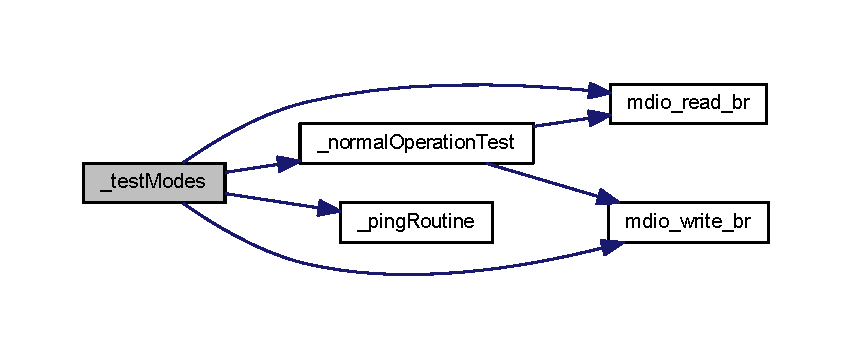
\includegraphics[width=350pt]{module_one_handle_routines_8c_a13ffca776e207f720598fece14e32d41_cgraph}
\end{center}
\end{figure}
\mbox{\Hypertarget{module_one_handle_routines_8c_a9d76ff69513e544453fdcbcb8fc5184c}\label{module_one_handle_routines_8c_a9d76ff69513e544453fdcbcb8fc5184c}} 
\index{module\+One\+Handle\+Routines.\+c@{module\+One\+Handle\+Routines.\+c}!module1\+\_\+\+Get\+Routine\+Num@{module1\+\_\+\+Get\+Routine\+Num}}
\index{module1\+\_\+\+Get\+Routine\+Num@{module1\+\_\+\+Get\+Routine\+Num}!module\+One\+Handle\+Routines.\+c@{module\+One\+Handle\+Routines.\+c}}
\subsubsection{\texorpdfstring{module1\+\_\+\+Get\+Routine\+Num()}{module1\_GetRoutineNum()}}
{\footnotesize\ttfamily void module1\+\_\+\+Get\+Routine\+Num (\begin{DoxyParamCaption}\item[{void}]{ }\end{DoxyParamCaption})}



This function gets number of routine which will be called and calls \mbox{\hyperlink{module_one_handle_routines_8c_a13ffca776e207f720598fece14e32d41}{\+\_\+test\+Modes(int routine\+\_\+trigger)}}. 

Here is the call graph for this function\+:
\nopagebreak
\begin{figure}[H]
\begin{center}
\leavevmode
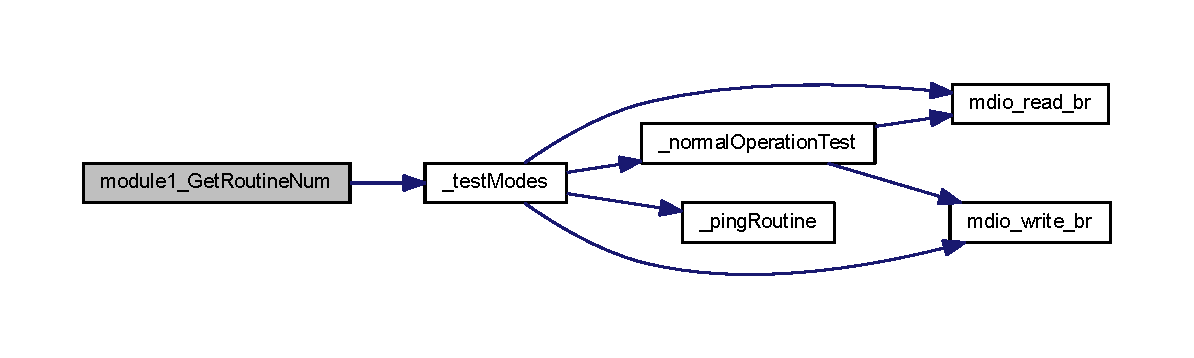
\includegraphics[width=350pt]{module_one_handle_routines_8c_a9d76ff69513e544453fdcbcb8fc5184c_cgraph}
\end{center}
\end{figure}

\hypertarget{module_one_handle_routines_8h}{}\section{module\+One\+Handle\+Routines.\+h File Reference}
\label{module_one_handle_routines_8h}\index{module\+One\+Handle\+Routines.\+h@{module\+One\+Handle\+Routines.\+h}}
This graph shows which files directly or indirectly include this file\+:\nopagebreak
\begin{figure}[H]
\begin{center}
\leavevmode
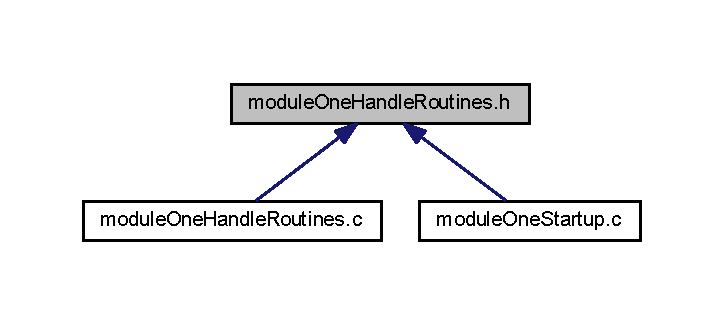
\includegraphics[width=348pt]{module_one_handle_routines_8h__dep__incl}
\end{center}
\end{figure}
\subsection*{Macros}
\begin{DoxyCompactItemize}
\item 
\#define \mbox{\hyperlink{module_one_handle_routines_8h_a1e27817ee436cbdeba83c2a35fe9cd44}{T\+A\+S\+K\+\_\+\+D\+E\+L\+A\+Y\+\_\+1000\+MS}}~(uint32\+\_\+t) (100\+U)
\item 
\#define \mbox{\hyperlink{module_one_handle_routines_8h_a306abfd62ab935890f8c4a226b7ce350}{P\+C\+\_\+\+I\+P\+V6}}~\char`\"{}fd53\+:7cb8\+:383\+:3\+::73\char`\"{}
\item 
\#define \mbox{\hyperlink{module_one_handle_routines_8h_a164477d7097713891f0cc021090deccb}{N\+U\+M\+\_\+\+O\+F\+\_\+\+P\+A\+C\+K\+E\+TS}}~((int8\+\_\+t) 4)
\item 
\#define \mbox{\hyperlink{module_one_handle_routines_8h_affbfbb29eccba558f22033239167d870}{E\+X\+T\+E\+N\+D\+E\+D\+\_\+\+C\+O\+N\+T\+R\+O\+L\+\_\+\+R\+E\+G\+I\+S\+T\+ER}}~((uint32\+\_\+t) (0x11))
\item 
\#define \mbox{\hyperlink{module_one_handle_routines_8h_ad6a5f0870f87a830a9281a48c20d1967}{C\+O\+N\+F\+I\+G\+U\+R\+A\+T\+I\+O\+N\+\_\+\+R\+E\+G\+I\+S\+T\+E\+R\+\_\+1}}~((uint32\+\_\+t) (0x12))
\item 
\#define \mbox{\hyperlink{module_one_handle_routines_8h_a94b832ef344b808412b6cab7113a8ff0}{G\+E\+N\+E\+R\+A\+L\+\_\+\+S\+T\+A\+T\+U\+S\+\_\+\+R\+EG}}~(0x18)
\item 
\#define \mbox{\hyperlink{module_one_handle_routines_8h_a18efc60ba4470dd61847046e7505e170}{L\+I\+N\+K\+\_\+\+F\+A\+I\+L\+\_\+\+C\+O\+U\+N\+T\+E\+R\+\_\+\+R\+EG}}~(0x1\+A)
\item 
\#define \mbox{\hyperlink{module_one_handle_routines_8h_a2b0cb97df82219fb79a4b81968bd7a68}{R\+E\+M\+\_\+\+R\+C\+V\+R\+\_\+\+C\+N\+T\+\_\+\+M\+A\+SK}}~(0x00\+F\+F\+U)
\item 
\#define \mbox{\hyperlink{module_one_handle_routines_8h_a27aedb47a9777cd1c22186aa3e56fbc8}{L\+O\+C\+\_\+\+R\+C\+V\+R\+\_\+\+C\+N\+T\+\_\+\+M\+A\+SK}}~(0x\+F\+F00\+U)
\item 
\#define \mbox{\hyperlink{module_one_handle_routines_8h_a0a49170f6977f14ccc80bfe320eafd79}{L\+I\+N\+K\+\_\+\+F\+A\+I\+L\+\_\+\+C\+N\+T\+\_\+\+M\+A\+SK}}~(0x00\+F8\+U)
\item 
\#define \mbox{\hyperlink{module_one_handle_routines_8h_a0dcb69692e9b1384ec75e8a3cc8588ae}{R\+O\+U\+T\+I\+N\+E\+\_\+\+I\+D\+LE}}~(0\+U)
\item 
\#define \mbox{\hyperlink{module_one_handle_routines_8h_a07b6ffef01524683d9b36ca3cb043c41}{R\+O\+U\+T\+I\+N\+E\+\_\+\+A\+C\+T\+I\+VE}}~(1\+U)
\item 
\#define \mbox{\hyperlink{module_one_handle_routines_8h_a60774b29047948527d01dedf09e0fe79}{R\+O\+U\+T\+I\+N\+E\+\_\+\+F\+I\+N\+I\+S\+H\+ED}}~(2\+U)
\item 
\#define \mbox{\hyperlink{module_one_handle_routines_8h_a29da6975d1cc044b60a246f08902382f}{R\+O\+U\+T\+I\+N\+E\+\_\+\+A\+B\+O\+R\+T\+ED}}~(3\+U)
\item 
\#define \mbox{\hyperlink{module_one_handle_routines_8h_a052107ec61fe05943ec49300675a43c7}{R\+O\+U\+T\+I\+N\+E\+\_\+\+I\+N\+C\+O\+R\+R\+E\+C\+T\+R\+E\+S\+U\+L\+TS}}~(0\+U)
\item 
\#define \mbox{\hyperlink{module_one_handle_routines_8h_a75f6d92f86998976324b2aeb5bf6f5a9}{R\+O\+U\+T\+I\+N\+E\+\_\+\+N\+O\+R\+E\+S\+U\+LT}}~(2\+U)
\item 
\#define \mbox{\hyperlink{module_one_handle_routines_8h_a71126f42da11e4f20ae19ada5d54c631}{R\+O\+U\+T\+I\+N\+E\+\_\+\+C\+O\+R\+R\+E\+C\+T\+R\+E\+S\+U\+L\+TS}}~(1\+U)
\item 
\#define \mbox{\hyperlink{module_one_handle_routines_8h_a01e01b6cdb1faa488c28b4b5ec2a2f6d}{R\+E\+A\+D\+\_\+\+L\+I\+N\+K\+\_\+\+F\+A\+IL}}~(7\+U)
\item 
\#define \mbox{\hyperlink{module_one_handle_routines_8h_a2afd4b5356c992007ffced26ca4f4bcd}{P\+I\+N\+G\+\_\+\+T\+E\+S\+T\+\_\+\+R\+O\+U\+T\+I\+NE}}~(6\+U)
\item 
\#define \mbox{\hyperlink{module_one_handle_routines_8h_a336342ef916d3e1e90b2139db8856ce6}{N\+O\+R\+M\+A\+L\+\_\+\+OP}}~(0\+U)
\item 
\#define \mbox{\hyperlink{module_one_handle_routines_8h_a3a7131c36aaab8dac8ab8766385c46c0}{S\+H\+I\+F\+T\+\_\+\+S\+IX}}~(6\+U)
\item 
\#define \mbox{\hyperlink{module_one_handle_routines_8h_a15cc231f70a38187f928ef8af427a8f1}{S\+H\+I\+F\+T\+\_\+\+T\+WO}}~(2\+U)
\item 
\#define \mbox{\hyperlink{module_one_handle_routines_8h_a0efb45398b365632ce15a87565c07330}{C\+O\+N\+F\+I\+G\+U\+R\+A\+T\+I\+O\+N\+\_\+\+R\+E\+G\+I\+S\+T\+E\+R\+\_\+\+A\+C\+C\+E\+S\+S\+\_\+\+E\+N\+A\+B\+L\+ED}}~(1\+U)
\end{DoxyCompactItemize}
\subsection*{Functions}
\begin{DoxyCompactItemize}
\item 
void \mbox{\hyperlink{module_one_handle_routines_8h_a9d76ff69513e544453fdcbcb8fc5184c}{module1\+\_\+\+Get\+Routine\+Num}} (void)
\begin{DoxyCompactList}\small\item\em This function gets number of routine which will be called and calls \mbox{\hyperlink{module_one_handle_routines_8c_a13ffca776e207f720598fece14e32d41}{\+\_\+test\+Modes(int routine\+\_\+trigger)}}. \end{DoxyCompactList}\end{DoxyCompactItemize}
\subsection*{Variables}
\begin{DoxyCompactItemize}
\item 
M\+S\+G\+\_\+\+Q\+\_\+\+ID \mbox{\hyperlink{module_one_handle_routines_8h_a7399395bce7dd3dd0341d0b7d7e78ec9}{routines\+Msg\+Q\+Id}}
\end{DoxyCompactItemize}


\subsection{Macro Definition Documentation}
\mbox{\Hypertarget{module_one_handle_routines_8h_ad6a5f0870f87a830a9281a48c20d1967}\label{module_one_handle_routines_8h_ad6a5f0870f87a830a9281a48c20d1967}} 
\index{module\+One\+Handle\+Routines.\+h@{module\+One\+Handle\+Routines.\+h}!C\+O\+N\+F\+I\+G\+U\+R\+A\+T\+I\+O\+N\+\_\+\+R\+E\+G\+I\+S\+T\+E\+R\+\_\+1@{C\+O\+N\+F\+I\+G\+U\+R\+A\+T\+I\+O\+N\+\_\+\+R\+E\+G\+I\+S\+T\+E\+R\+\_\+1}}
\index{C\+O\+N\+F\+I\+G\+U\+R\+A\+T\+I\+O\+N\+\_\+\+R\+E\+G\+I\+S\+T\+E\+R\+\_\+1@{C\+O\+N\+F\+I\+G\+U\+R\+A\+T\+I\+O\+N\+\_\+\+R\+E\+G\+I\+S\+T\+E\+R\+\_\+1}!module\+One\+Handle\+Routines.\+h@{module\+One\+Handle\+Routines.\+h}}
\subsubsection{\texorpdfstring{C\+O\+N\+F\+I\+G\+U\+R\+A\+T\+I\+O\+N\+\_\+\+R\+E\+G\+I\+S\+T\+E\+R\+\_\+1}{CONFIGURATION\_REGISTER\_1}}
{\footnotesize\ttfamily \#define C\+O\+N\+F\+I\+G\+U\+R\+A\+T\+I\+O\+N\+\_\+\+R\+E\+G\+I\+S\+T\+E\+R\+\_\+1~((uint32\+\_\+t) (0x12))}

\mbox{\Hypertarget{module_one_handle_routines_8h_a0efb45398b365632ce15a87565c07330}\label{module_one_handle_routines_8h_a0efb45398b365632ce15a87565c07330}} 
\index{module\+One\+Handle\+Routines.\+h@{module\+One\+Handle\+Routines.\+h}!C\+O\+N\+F\+I\+G\+U\+R\+A\+T\+I\+O\+N\+\_\+\+R\+E\+G\+I\+S\+T\+E\+R\+\_\+\+A\+C\+C\+E\+S\+S\+\_\+\+E\+N\+A\+B\+L\+ED@{C\+O\+N\+F\+I\+G\+U\+R\+A\+T\+I\+O\+N\+\_\+\+R\+E\+G\+I\+S\+T\+E\+R\+\_\+\+A\+C\+C\+E\+S\+S\+\_\+\+E\+N\+A\+B\+L\+ED}}
\index{C\+O\+N\+F\+I\+G\+U\+R\+A\+T\+I\+O\+N\+\_\+\+R\+E\+G\+I\+S\+T\+E\+R\+\_\+\+A\+C\+C\+E\+S\+S\+\_\+\+E\+N\+A\+B\+L\+ED@{C\+O\+N\+F\+I\+G\+U\+R\+A\+T\+I\+O\+N\+\_\+\+R\+E\+G\+I\+S\+T\+E\+R\+\_\+\+A\+C\+C\+E\+S\+S\+\_\+\+E\+N\+A\+B\+L\+ED}!module\+One\+Handle\+Routines.\+h@{module\+One\+Handle\+Routines.\+h}}
\subsubsection{\texorpdfstring{C\+O\+N\+F\+I\+G\+U\+R\+A\+T\+I\+O\+N\+\_\+\+R\+E\+G\+I\+S\+T\+E\+R\+\_\+\+A\+C\+C\+E\+S\+S\+\_\+\+E\+N\+A\+B\+L\+ED}{CONFIGURATION\_REGISTER\_ACCESS\_ENABLED}}
{\footnotesize\ttfamily \#define C\+O\+N\+F\+I\+G\+U\+R\+A\+T\+I\+O\+N\+\_\+\+R\+E\+G\+I\+S\+T\+E\+R\+\_\+\+A\+C\+C\+E\+S\+S\+\_\+\+E\+N\+A\+B\+L\+ED~(1\+U)}

\mbox{\Hypertarget{module_one_handle_routines_8h_affbfbb29eccba558f22033239167d870}\label{module_one_handle_routines_8h_affbfbb29eccba558f22033239167d870}} 
\index{module\+One\+Handle\+Routines.\+h@{module\+One\+Handle\+Routines.\+h}!E\+X\+T\+E\+N\+D\+E\+D\+\_\+\+C\+O\+N\+T\+R\+O\+L\+\_\+\+R\+E\+G\+I\+S\+T\+ER@{E\+X\+T\+E\+N\+D\+E\+D\+\_\+\+C\+O\+N\+T\+R\+O\+L\+\_\+\+R\+E\+G\+I\+S\+T\+ER}}
\index{E\+X\+T\+E\+N\+D\+E\+D\+\_\+\+C\+O\+N\+T\+R\+O\+L\+\_\+\+R\+E\+G\+I\+S\+T\+ER@{E\+X\+T\+E\+N\+D\+E\+D\+\_\+\+C\+O\+N\+T\+R\+O\+L\+\_\+\+R\+E\+G\+I\+S\+T\+ER}!module\+One\+Handle\+Routines.\+h@{module\+One\+Handle\+Routines.\+h}}
\subsubsection{\texorpdfstring{E\+X\+T\+E\+N\+D\+E\+D\+\_\+\+C\+O\+N\+T\+R\+O\+L\+\_\+\+R\+E\+G\+I\+S\+T\+ER}{EXTENDED\_CONTROL\_REGISTER}}
{\footnotesize\ttfamily \#define E\+X\+T\+E\+N\+D\+E\+D\+\_\+\+C\+O\+N\+T\+R\+O\+L\+\_\+\+R\+E\+G\+I\+S\+T\+ER~((uint32\+\_\+t) (0x11))}

\mbox{\Hypertarget{module_one_handle_routines_8h_a94b832ef344b808412b6cab7113a8ff0}\label{module_one_handle_routines_8h_a94b832ef344b808412b6cab7113a8ff0}} 
\index{module\+One\+Handle\+Routines.\+h@{module\+One\+Handle\+Routines.\+h}!G\+E\+N\+E\+R\+A\+L\+\_\+\+S\+T\+A\+T\+U\+S\+\_\+\+R\+EG@{G\+E\+N\+E\+R\+A\+L\+\_\+\+S\+T\+A\+T\+U\+S\+\_\+\+R\+EG}}
\index{G\+E\+N\+E\+R\+A\+L\+\_\+\+S\+T\+A\+T\+U\+S\+\_\+\+R\+EG@{G\+E\+N\+E\+R\+A\+L\+\_\+\+S\+T\+A\+T\+U\+S\+\_\+\+R\+EG}!module\+One\+Handle\+Routines.\+h@{module\+One\+Handle\+Routines.\+h}}
\subsubsection{\texorpdfstring{G\+E\+N\+E\+R\+A\+L\+\_\+\+S\+T\+A\+T\+U\+S\+\_\+\+R\+EG}{GENERAL\_STATUS\_REG}}
{\footnotesize\ttfamily \#define G\+E\+N\+E\+R\+A\+L\+\_\+\+S\+T\+A\+T\+U\+S\+\_\+\+R\+EG~(0x18)}

\mbox{\Hypertarget{module_one_handle_routines_8h_a0a49170f6977f14ccc80bfe320eafd79}\label{module_one_handle_routines_8h_a0a49170f6977f14ccc80bfe320eafd79}} 
\index{module\+One\+Handle\+Routines.\+h@{module\+One\+Handle\+Routines.\+h}!L\+I\+N\+K\+\_\+\+F\+A\+I\+L\+\_\+\+C\+N\+T\+\_\+\+M\+A\+SK@{L\+I\+N\+K\+\_\+\+F\+A\+I\+L\+\_\+\+C\+N\+T\+\_\+\+M\+A\+SK}}
\index{L\+I\+N\+K\+\_\+\+F\+A\+I\+L\+\_\+\+C\+N\+T\+\_\+\+M\+A\+SK@{L\+I\+N\+K\+\_\+\+F\+A\+I\+L\+\_\+\+C\+N\+T\+\_\+\+M\+A\+SK}!module\+One\+Handle\+Routines.\+h@{module\+One\+Handle\+Routines.\+h}}
\subsubsection{\texorpdfstring{L\+I\+N\+K\+\_\+\+F\+A\+I\+L\+\_\+\+C\+N\+T\+\_\+\+M\+A\+SK}{LINK\_FAIL\_CNT\_MASK}}
{\footnotesize\ttfamily \#define L\+I\+N\+K\+\_\+\+F\+A\+I\+L\+\_\+\+C\+N\+T\+\_\+\+M\+A\+SK~(0x00\+F8\+U)}

\mbox{\Hypertarget{module_one_handle_routines_8h_a18efc60ba4470dd61847046e7505e170}\label{module_one_handle_routines_8h_a18efc60ba4470dd61847046e7505e170}} 
\index{module\+One\+Handle\+Routines.\+h@{module\+One\+Handle\+Routines.\+h}!L\+I\+N\+K\+\_\+\+F\+A\+I\+L\+\_\+\+C\+O\+U\+N\+T\+E\+R\+\_\+\+R\+EG@{L\+I\+N\+K\+\_\+\+F\+A\+I\+L\+\_\+\+C\+O\+U\+N\+T\+E\+R\+\_\+\+R\+EG}}
\index{L\+I\+N\+K\+\_\+\+F\+A\+I\+L\+\_\+\+C\+O\+U\+N\+T\+E\+R\+\_\+\+R\+EG@{L\+I\+N\+K\+\_\+\+F\+A\+I\+L\+\_\+\+C\+O\+U\+N\+T\+E\+R\+\_\+\+R\+EG}!module\+One\+Handle\+Routines.\+h@{module\+One\+Handle\+Routines.\+h}}
\subsubsection{\texorpdfstring{L\+I\+N\+K\+\_\+\+F\+A\+I\+L\+\_\+\+C\+O\+U\+N\+T\+E\+R\+\_\+\+R\+EG}{LINK\_FAIL\_COUNTER\_REG}}
{\footnotesize\ttfamily \#define L\+I\+N\+K\+\_\+\+F\+A\+I\+L\+\_\+\+C\+O\+U\+N\+T\+E\+R\+\_\+\+R\+EG~(0x1\+A)}

\mbox{\Hypertarget{module_one_handle_routines_8h_a27aedb47a9777cd1c22186aa3e56fbc8}\label{module_one_handle_routines_8h_a27aedb47a9777cd1c22186aa3e56fbc8}} 
\index{module\+One\+Handle\+Routines.\+h@{module\+One\+Handle\+Routines.\+h}!L\+O\+C\+\_\+\+R\+C\+V\+R\+\_\+\+C\+N\+T\+\_\+\+M\+A\+SK@{L\+O\+C\+\_\+\+R\+C\+V\+R\+\_\+\+C\+N\+T\+\_\+\+M\+A\+SK}}
\index{L\+O\+C\+\_\+\+R\+C\+V\+R\+\_\+\+C\+N\+T\+\_\+\+M\+A\+SK@{L\+O\+C\+\_\+\+R\+C\+V\+R\+\_\+\+C\+N\+T\+\_\+\+M\+A\+SK}!module\+One\+Handle\+Routines.\+h@{module\+One\+Handle\+Routines.\+h}}
\subsubsection{\texorpdfstring{L\+O\+C\+\_\+\+R\+C\+V\+R\+\_\+\+C\+N\+T\+\_\+\+M\+A\+SK}{LOC\_RCVR\_CNT\_MASK}}
{\footnotesize\ttfamily \#define L\+O\+C\+\_\+\+R\+C\+V\+R\+\_\+\+C\+N\+T\+\_\+\+M\+A\+SK~(0x\+F\+F00\+U)}

\mbox{\Hypertarget{module_one_handle_routines_8h_a336342ef916d3e1e90b2139db8856ce6}\label{module_one_handle_routines_8h_a336342ef916d3e1e90b2139db8856ce6}} 
\index{module\+One\+Handle\+Routines.\+h@{module\+One\+Handle\+Routines.\+h}!N\+O\+R\+M\+A\+L\+\_\+\+OP@{N\+O\+R\+M\+A\+L\+\_\+\+OP}}
\index{N\+O\+R\+M\+A\+L\+\_\+\+OP@{N\+O\+R\+M\+A\+L\+\_\+\+OP}!module\+One\+Handle\+Routines.\+h@{module\+One\+Handle\+Routines.\+h}}
\subsubsection{\texorpdfstring{N\+O\+R\+M\+A\+L\+\_\+\+OP}{NORMAL\_OP}}
{\footnotesize\ttfamily \#define N\+O\+R\+M\+A\+L\+\_\+\+OP~(0\+U)}

\mbox{\Hypertarget{module_one_handle_routines_8h_a164477d7097713891f0cc021090deccb}\label{module_one_handle_routines_8h_a164477d7097713891f0cc021090deccb}} 
\index{module\+One\+Handle\+Routines.\+h@{module\+One\+Handle\+Routines.\+h}!N\+U\+M\+\_\+\+O\+F\+\_\+\+P\+A\+C\+K\+E\+TS@{N\+U\+M\+\_\+\+O\+F\+\_\+\+P\+A\+C\+K\+E\+TS}}
\index{N\+U\+M\+\_\+\+O\+F\+\_\+\+P\+A\+C\+K\+E\+TS@{N\+U\+M\+\_\+\+O\+F\+\_\+\+P\+A\+C\+K\+E\+TS}!module\+One\+Handle\+Routines.\+h@{module\+One\+Handle\+Routines.\+h}}
\subsubsection{\texorpdfstring{N\+U\+M\+\_\+\+O\+F\+\_\+\+P\+A\+C\+K\+E\+TS}{NUM\_OF\_PACKETS}}
{\footnotesize\ttfamily \#define N\+U\+M\+\_\+\+O\+F\+\_\+\+P\+A\+C\+K\+E\+TS~((int8\+\_\+t) 4)}

\mbox{\Hypertarget{module_one_handle_routines_8h_a306abfd62ab935890f8c4a226b7ce350}\label{module_one_handle_routines_8h_a306abfd62ab935890f8c4a226b7ce350}} 
\index{module\+One\+Handle\+Routines.\+h@{module\+One\+Handle\+Routines.\+h}!P\+C\+\_\+\+I\+P\+V6@{P\+C\+\_\+\+I\+P\+V6}}
\index{P\+C\+\_\+\+I\+P\+V6@{P\+C\+\_\+\+I\+P\+V6}!module\+One\+Handle\+Routines.\+h@{module\+One\+Handle\+Routines.\+h}}
\subsubsection{\texorpdfstring{P\+C\+\_\+\+I\+P\+V6}{PC\_IPV6}}
{\footnotesize\ttfamily \#define P\+C\+\_\+\+I\+P\+V6~\char`\"{}fd53\+:7cb8\+:383\+:3\+::73\char`\"{}}

\mbox{\Hypertarget{module_one_handle_routines_8h_a2afd4b5356c992007ffced26ca4f4bcd}\label{module_one_handle_routines_8h_a2afd4b5356c992007ffced26ca4f4bcd}} 
\index{module\+One\+Handle\+Routines.\+h@{module\+One\+Handle\+Routines.\+h}!P\+I\+N\+G\+\_\+\+T\+E\+S\+T\+\_\+\+R\+O\+U\+T\+I\+NE@{P\+I\+N\+G\+\_\+\+T\+E\+S\+T\+\_\+\+R\+O\+U\+T\+I\+NE}}
\index{P\+I\+N\+G\+\_\+\+T\+E\+S\+T\+\_\+\+R\+O\+U\+T\+I\+NE@{P\+I\+N\+G\+\_\+\+T\+E\+S\+T\+\_\+\+R\+O\+U\+T\+I\+NE}!module\+One\+Handle\+Routines.\+h@{module\+One\+Handle\+Routines.\+h}}
\subsubsection{\texorpdfstring{P\+I\+N\+G\+\_\+\+T\+E\+S\+T\+\_\+\+R\+O\+U\+T\+I\+NE}{PING\_TEST\_ROUTINE}}
{\footnotesize\ttfamily \#define P\+I\+N\+G\+\_\+\+T\+E\+S\+T\+\_\+\+R\+O\+U\+T\+I\+NE~(6\+U)}

\mbox{\Hypertarget{module_one_handle_routines_8h_a01e01b6cdb1faa488c28b4b5ec2a2f6d}\label{module_one_handle_routines_8h_a01e01b6cdb1faa488c28b4b5ec2a2f6d}} 
\index{module\+One\+Handle\+Routines.\+h@{module\+One\+Handle\+Routines.\+h}!R\+E\+A\+D\+\_\+\+L\+I\+N\+K\+\_\+\+F\+A\+IL@{R\+E\+A\+D\+\_\+\+L\+I\+N\+K\+\_\+\+F\+A\+IL}}
\index{R\+E\+A\+D\+\_\+\+L\+I\+N\+K\+\_\+\+F\+A\+IL@{R\+E\+A\+D\+\_\+\+L\+I\+N\+K\+\_\+\+F\+A\+IL}!module\+One\+Handle\+Routines.\+h@{module\+One\+Handle\+Routines.\+h}}
\subsubsection{\texorpdfstring{R\+E\+A\+D\+\_\+\+L\+I\+N\+K\+\_\+\+F\+A\+IL}{READ\_LINK\_FAIL}}
{\footnotesize\ttfamily \#define R\+E\+A\+D\+\_\+\+L\+I\+N\+K\+\_\+\+F\+A\+IL~(7\+U)}

\mbox{\Hypertarget{module_one_handle_routines_8h_a2b0cb97df82219fb79a4b81968bd7a68}\label{module_one_handle_routines_8h_a2b0cb97df82219fb79a4b81968bd7a68}} 
\index{module\+One\+Handle\+Routines.\+h@{module\+One\+Handle\+Routines.\+h}!R\+E\+M\+\_\+\+R\+C\+V\+R\+\_\+\+C\+N\+T\+\_\+\+M\+A\+SK@{R\+E\+M\+\_\+\+R\+C\+V\+R\+\_\+\+C\+N\+T\+\_\+\+M\+A\+SK}}
\index{R\+E\+M\+\_\+\+R\+C\+V\+R\+\_\+\+C\+N\+T\+\_\+\+M\+A\+SK@{R\+E\+M\+\_\+\+R\+C\+V\+R\+\_\+\+C\+N\+T\+\_\+\+M\+A\+SK}!module\+One\+Handle\+Routines.\+h@{module\+One\+Handle\+Routines.\+h}}
\subsubsection{\texorpdfstring{R\+E\+M\+\_\+\+R\+C\+V\+R\+\_\+\+C\+N\+T\+\_\+\+M\+A\+SK}{REM\_RCVR\_CNT\_MASK}}
{\footnotesize\ttfamily \#define R\+E\+M\+\_\+\+R\+C\+V\+R\+\_\+\+C\+N\+T\+\_\+\+M\+A\+SK~(0x00\+F\+F\+U)}

\mbox{\Hypertarget{module_one_handle_routines_8h_a29da6975d1cc044b60a246f08902382f}\label{module_one_handle_routines_8h_a29da6975d1cc044b60a246f08902382f}} 
\index{module\+One\+Handle\+Routines.\+h@{module\+One\+Handle\+Routines.\+h}!R\+O\+U\+T\+I\+N\+E\+\_\+\+A\+B\+O\+R\+T\+ED@{R\+O\+U\+T\+I\+N\+E\+\_\+\+A\+B\+O\+R\+T\+ED}}
\index{R\+O\+U\+T\+I\+N\+E\+\_\+\+A\+B\+O\+R\+T\+ED@{R\+O\+U\+T\+I\+N\+E\+\_\+\+A\+B\+O\+R\+T\+ED}!module\+One\+Handle\+Routines.\+h@{module\+One\+Handle\+Routines.\+h}}
\subsubsection{\texorpdfstring{R\+O\+U\+T\+I\+N\+E\+\_\+\+A\+B\+O\+R\+T\+ED}{ROUTINE\_ABORTED}}
{\footnotesize\ttfamily \#define R\+O\+U\+T\+I\+N\+E\+\_\+\+A\+B\+O\+R\+T\+ED~(3\+U)}

\mbox{\Hypertarget{module_one_handle_routines_8h_a07b6ffef01524683d9b36ca3cb043c41}\label{module_one_handle_routines_8h_a07b6ffef01524683d9b36ca3cb043c41}} 
\index{module\+One\+Handle\+Routines.\+h@{module\+One\+Handle\+Routines.\+h}!R\+O\+U\+T\+I\+N\+E\+\_\+\+A\+C\+T\+I\+VE@{R\+O\+U\+T\+I\+N\+E\+\_\+\+A\+C\+T\+I\+VE}}
\index{R\+O\+U\+T\+I\+N\+E\+\_\+\+A\+C\+T\+I\+VE@{R\+O\+U\+T\+I\+N\+E\+\_\+\+A\+C\+T\+I\+VE}!module\+One\+Handle\+Routines.\+h@{module\+One\+Handle\+Routines.\+h}}
\subsubsection{\texorpdfstring{R\+O\+U\+T\+I\+N\+E\+\_\+\+A\+C\+T\+I\+VE}{ROUTINE\_ACTIVE}}
{\footnotesize\ttfamily \#define R\+O\+U\+T\+I\+N\+E\+\_\+\+A\+C\+T\+I\+VE~(1\+U)}

\mbox{\Hypertarget{module_one_handle_routines_8h_a71126f42da11e4f20ae19ada5d54c631}\label{module_one_handle_routines_8h_a71126f42da11e4f20ae19ada5d54c631}} 
\index{module\+One\+Handle\+Routines.\+h@{module\+One\+Handle\+Routines.\+h}!R\+O\+U\+T\+I\+N\+E\+\_\+\+C\+O\+R\+R\+E\+C\+T\+R\+E\+S\+U\+L\+TS@{R\+O\+U\+T\+I\+N\+E\+\_\+\+C\+O\+R\+R\+E\+C\+T\+R\+E\+S\+U\+L\+TS}}
\index{R\+O\+U\+T\+I\+N\+E\+\_\+\+C\+O\+R\+R\+E\+C\+T\+R\+E\+S\+U\+L\+TS@{R\+O\+U\+T\+I\+N\+E\+\_\+\+C\+O\+R\+R\+E\+C\+T\+R\+E\+S\+U\+L\+TS}!module\+One\+Handle\+Routines.\+h@{module\+One\+Handle\+Routines.\+h}}
\subsubsection{\texorpdfstring{R\+O\+U\+T\+I\+N\+E\+\_\+\+C\+O\+R\+R\+E\+C\+T\+R\+E\+S\+U\+L\+TS}{ROUTINE\_CORRECTRESULTS}}
{\footnotesize\ttfamily \#define R\+O\+U\+T\+I\+N\+E\+\_\+\+C\+O\+R\+R\+E\+C\+T\+R\+E\+S\+U\+L\+TS~(1\+U)}

\mbox{\Hypertarget{module_one_handle_routines_8h_a60774b29047948527d01dedf09e0fe79}\label{module_one_handle_routines_8h_a60774b29047948527d01dedf09e0fe79}} 
\index{module\+One\+Handle\+Routines.\+h@{module\+One\+Handle\+Routines.\+h}!R\+O\+U\+T\+I\+N\+E\+\_\+\+F\+I\+N\+I\+S\+H\+ED@{R\+O\+U\+T\+I\+N\+E\+\_\+\+F\+I\+N\+I\+S\+H\+ED}}
\index{R\+O\+U\+T\+I\+N\+E\+\_\+\+F\+I\+N\+I\+S\+H\+ED@{R\+O\+U\+T\+I\+N\+E\+\_\+\+F\+I\+N\+I\+S\+H\+ED}!module\+One\+Handle\+Routines.\+h@{module\+One\+Handle\+Routines.\+h}}
\subsubsection{\texorpdfstring{R\+O\+U\+T\+I\+N\+E\+\_\+\+F\+I\+N\+I\+S\+H\+ED}{ROUTINE\_FINISHED}}
{\footnotesize\ttfamily \#define R\+O\+U\+T\+I\+N\+E\+\_\+\+F\+I\+N\+I\+S\+H\+ED~(2\+U)}

\mbox{\Hypertarget{module_one_handle_routines_8h_a0dcb69692e9b1384ec75e8a3cc8588ae}\label{module_one_handle_routines_8h_a0dcb69692e9b1384ec75e8a3cc8588ae}} 
\index{module\+One\+Handle\+Routines.\+h@{module\+One\+Handle\+Routines.\+h}!R\+O\+U\+T\+I\+N\+E\+\_\+\+I\+D\+LE@{R\+O\+U\+T\+I\+N\+E\+\_\+\+I\+D\+LE}}
\index{R\+O\+U\+T\+I\+N\+E\+\_\+\+I\+D\+LE@{R\+O\+U\+T\+I\+N\+E\+\_\+\+I\+D\+LE}!module\+One\+Handle\+Routines.\+h@{module\+One\+Handle\+Routines.\+h}}
\subsubsection{\texorpdfstring{R\+O\+U\+T\+I\+N\+E\+\_\+\+I\+D\+LE}{ROUTINE\_IDLE}}
{\footnotesize\ttfamily \#define R\+O\+U\+T\+I\+N\+E\+\_\+\+I\+D\+LE~(0\+U)}

\mbox{\Hypertarget{module_one_handle_routines_8h_a052107ec61fe05943ec49300675a43c7}\label{module_one_handle_routines_8h_a052107ec61fe05943ec49300675a43c7}} 
\index{module\+One\+Handle\+Routines.\+h@{module\+One\+Handle\+Routines.\+h}!R\+O\+U\+T\+I\+N\+E\+\_\+\+I\+N\+C\+O\+R\+R\+E\+C\+T\+R\+E\+S\+U\+L\+TS@{R\+O\+U\+T\+I\+N\+E\+\_\+\+I\+N\+C\+O\+R\+R\+E\+C\+T\+R\+E\+S\+U\+L\+TS}}
\index{R\+O\+U\+T\+I\+N\+E\+\_\+\+I\+N\+C\+O\+R\+R\+E\+C\+T\+R\+E\+S\+U\+L\+TS@{R\+O\+U\+T\+I\+N\+E\+\_\+\+I\+N\+C\+O\+R\+R\+E\+C\+T\+R\+E\+S\+U\+L\+TS}!module\+One\+Handle\+Routines.\+h@{module\+One\+Handle\+Routines.\+h}}
\subsubsection{\texorpdfstring{R\+O\+U\+T\+I\+N\+E\+\_\+\+I\+N\+C\+O\+R\+R\+E\+C\+T\+R\+E\+S\+U\+L\+TS}{ROUTINE\_INCORRECTRESULTS}}
{\footnotesize\ttfamily \#define R\+O\+U\+T\+I\+N\+E\+\_\+\+I\+N\+C\+O\+R\+R\+E\+C\+T\+R\+E\+S\+U\+L\+TS~(0\+U)}

\mbox{\Hypertarget{module_one_handle_routines_8h_a75f6d92f86998976324b2aeb5bf6f5a9}\label{module_one_handle_routines_8h_a75f6d92f86998976324b2aeb5bf6f5a9}} 
\index{module\+One\+Handle\+Routines.\+h@{module\+One\+Handle\+Routines.\+h}!R\+O\+U\+T\+I\+N\+E\+\_\+\+N\+O\+R\+E\+S\+U\+LT@{R\+O\+U\+T\+I\+N\+E\+\_\+\+N\+O\+R\+E\+S\+U\+LT}}
\index{R\+O\+U\+T\+I\+N\+E\+\_\+\+N\+O\+R\+E\+S\+U\+LT@{R\+O\+U\+T\+I\+N\+E\+\_\+\+N\+O\+R\+E\+S\+U\+LT}!module\+One\+Handle\+Routines.\+h@{module\+One\+Handle\+Routines.\+h}}
\subsubsection{\texorpdfstring{R\+O\+U\+T\+I\+N\+E\+\_\+\+N\+O\+R\+E\+S\+U\+LT}{ROUTINE\_NORESULT}}
{\footnotesize\ttfamily \#define R\+O\+U\+T\+I\+N\+E\+\_\+\+N\+O\+R\+E\+S\+U\+LT~(2\+U)}

\mbox{\Hypertarget{module_one_handle_routines_8h_a3a7131c36aaab8dac8ab8766385c46c0}\label{module_one_handle_routines_8h_a3a7131c36aaab8dac8ab8766385c46c0}} 
\index{module\+One\+Handle\+Routines.\+h@{module\+One\+Handle\+Routines.\+h}!S\+H\+I\+F\+T\+\_\+\+S\+IX@{S\+H\+I\+F\+T\+\_\+\+S\+IX}}
\index{S\+H\+I\+F\+T\+\_\+\+S\+IX@{S\+H\+I\+F\+T\+\_\+\+S\+IX}!module\+One\+Handle\+Routines.\+h@{module\+One\+Handle\+Routines.\+h}}
\subsubsection{\texorpdfstring{S\+H\+I\+F\+T\+\_\+\+S\+IX}{SHIFT\_SIX}}
{\footnotesize\ttfamily \#define S\+H\+I\+F\+T\+\_\+\+S\+IX~(6\+U)}

\mbox{\Hypertarget{module_one_handle_routines_8h_a15cc231f70a38187f928ef8af427a8f1}\label{module_one_handle_routines_8h_a15cc231f70a38187f928ef8af427a8f1}} 
\index{module\+One\+Handle\+Routines.\+h@{module\+One\+Handle\+Routines.\+h}!S\+H\+I\+F\+T\+\_\+\+T\+WO@{S\+H\+I\+F\+T\+\_\+\+T\+WO}}
\index{S\+H\+I\+F\+T\+\_\+\+T\+WO@{S\+H\+I\+F\+T\+\_\+\+T\+WO}!module\+One\+Handle\+Routines.\+h@{module\+One\+Handle\+Routines.\+h}}
\subsubsection{\texorpdfstring{S\+H\+I\+F\+T\+\_\+\+T\+WO}{SHIFT\_TWO}}
{\footnotesize\ttfamily \#define S\+H\+I\+F\+T\+\_\+\+T\+WO~(2\+U)}

\mbox{\Hypertarget{module_one_handle_routines_8h_a1e27817ee436cbdeba83c2a35fe9cd44}\label{module_one_handle_routines_8h_a1e27817ee436cbdeba83c2a35fe9cd44}} 
\index{module\+One\+Handle\+Routines.\+h@{module\+One\+Handle\+Routines.\+h}!T\+A\+S\+K\+\_\+\+D\+E\+L\+A\+Y\+\_\+1000\+MS@{T\+A\+S\+K\+\_\+\+D\+E\+L\+A\+Y\+\_\+1000\+MS}}
\index{T\+A\+S\+K\+\_\+\+D\+E\+L\+A\+Y\+\_\+1000\+MS@{T\+A\+S\+K\+\_\+\+D\+E\+L\+A\+Y\+\_\+1000\+MS}!module\+One\+Handle\+Routines.\+h@{module\+One\+Handle\+Routines.\+h}}
\subsubsection{\texorpdfstring{T\+A\+S\+K\+\_\+\+D\+E\+L\+A\+Y\+\_\+1000\+MS}{TASK\_DELAY\_1000MS}}
{\footnotesize\ttfamily \#define T\+A\+S\+K\+\_\+\+D\+E\+L\+A\+Y\+\_\+1000\+MS~(uint32\+\_\+t) (100\+U)}



\subsection{Function Documentation}
\mbox{\Hypertarget{module_one_handle_routines_8h_a9d76ff69513e544453fdcbcb8fc5184c}\label{module_one_handle_routines_8h_a9d76ff69513e544453fdcbcb8fc5184c}} 
\index{module\+One\+Handle\+Routines.\+h@{module\+One\+Handle\+Routines.\+h}!module1\+\_\+\+Get\+Routine\+Num@{module1\+\_\+\+Get\+Routine\+Num}}
\index{module1\+\_\+\+Get\+Routine\+Num@{module1\+\_\+\+Get\+Routine\+Num}!module\+One\+Handle\+Routines.\+h@{module\+One\+Handle\+Routines.\+h}}
\subsubsection{\texorpdfstring{module1\+\_\+\+Get\+Routine\+Num()}{module1\_GetRoutineNum()}}
{\footnotesize\ttfamily void module1\+\_\+\+Get\+Routine\+Num (\begin{DoxyParamCaption}\item[{void}]{ }\end{DoxyParamCaption})}



This function gets number of routine which will be called and calls \mbox{\hyperlink{module_one_handle_routines_8c_a13ffca776e207f720598fece14e32d41}{\+\_\+test\+Modes(int routine\+\_\+trigger)}}. 

Here is the call graph for this function\+:\nopagebreak
\begin{figure}[H]
\begin{center}
\leavevmode
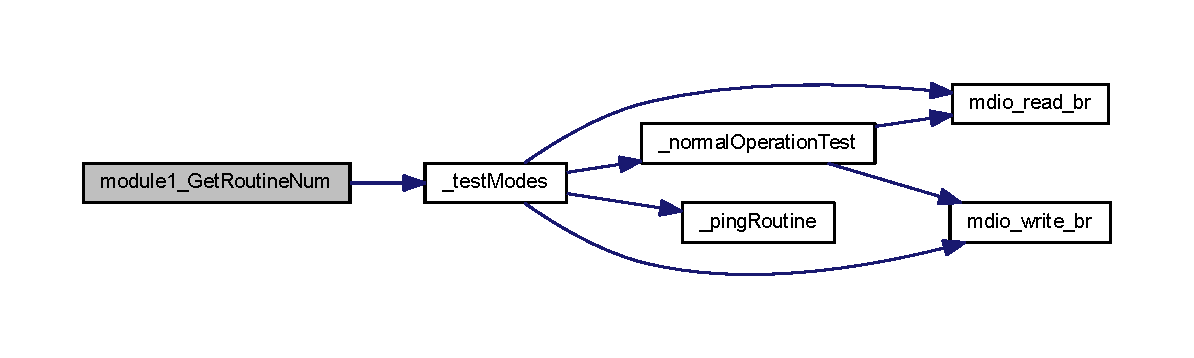
\includegraphics[width=350pt]{module_one_handle_routines_8h_a9d76ff69513e544453fdcbcb8fc5184c_cgraph}
\end{center}
\end{figure}


\subsection{Variable Documentation}
\mbox{\Hypertarget{module_one_handle_routines_8h_a7399395bce7dd3dd0341d0b7d7e78ec9}\label{module_one_handle_routines_8h_a7399395bce7dd3dd0341d0b7d7e78ec9}} 
\index{module\+One\+Handle\+Routines.\+h@{module\+One\+Handle\+Routines.\+h}!routines\+Msg\+Q\+Id@{routines\+Msg\+Q\+Id}}
\index{routines\+Msg\+Q\+Id@{routines\+Msg\+Q\+Id}!module\+One\+Handle\+Routines.\+h@{module\+One\+Handle\+Routines.\+h}}
\subsubsection{\texorpdfstring{routines\+Msg\+Q\+Id}{routinesMsgQId}}
{\footnotesize\ttfamily M\+S\+G\+\_\+\+Q\+\_\+\+ID routines\+Msg\+Q\+Id}


\hypertarget{module_one_read_eth_phy_8c}{}\section{module\+One\+Read\+Eth\+Phy.\+c File Reference}
\label{module_one_read_eth_phy_8c}\index{module\+One\+Read\+Eth\+Phy.\+c@{module\+One\+Read\+Eth\+Phy.\+c}}


Functions to read and write in T\+J\+A1100 registers and functions that fill shared memory and message queue with diagnostic data.  


{\ttfamily \#include $<$vxworks.\+h$>$}\newline
{\ttfamily \#include $<$stdio.\+h$>$}\newline
{\ttfamily \#include $<$mem\+Lib.\+h$>$}\newline
{\ttfamily \#include $<$pmap\+Lib.\+h$>$}\newline
{\ttfamily \#include $<$vm\+Lib\+Common.\+h$>$}\newline
{\ttfamily \#include $<$msg\+Q\+Lib\+Common.\+h$>$}\newline
{\ttfamily \#include $<$task\+Lib\+Common.\+h$>$}\newline
{\ttfamily \#include $<$time.\+h$>$}\newline
{\ttfamily \#include $<$string.\+h$>$}\newline
{\ttfamily \#include $<$sys/mman.\+h$>$}\newline
{\ttfamily \#include $<$unistd.\+h$>$}\newline
{\ttfamily \#include $<$net/utils/ifconfig.\+h$>$}\newline
{\ttfamily \#include $<$sys/fcntlcom.\+h$>$}\newline
{\ttfamily \#include $<$stat.\+h$>$}\newline
{\ttfamily \#include \char`\"{}module\+One\+Read\+Eth\+Phy.\+h\char`\"{}}\newline
Include dependency graph for module\+One\+Read\+Eth\+Phy.\+c\+:\nopagebreak
\begin{figure}[H]
\begin{center}
\leavevmode
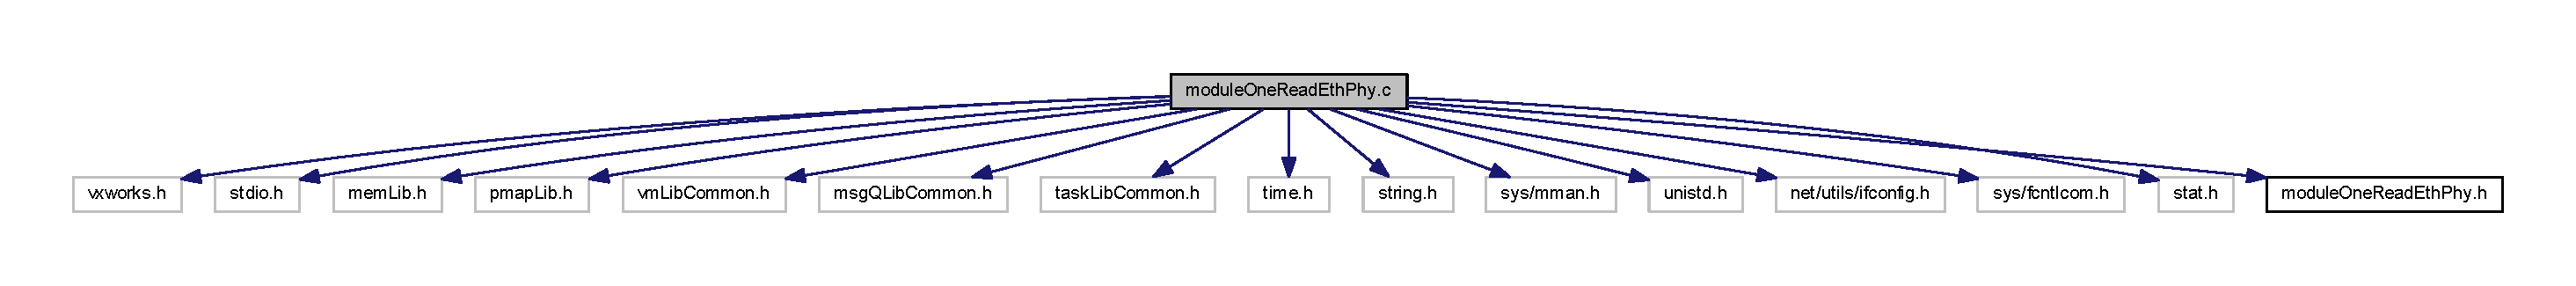
\includegraphics[width=350pt]{module_one_read_eth_phy_8c__incl}
\end{center}
\end{figure}
\subsection*{Functions}
\begin{DoxyCompactItemize}
\item 
L\+O\+C\+AL void \mbox{\hyperlink{module_one_read_eth_phy_8c_ad3d33414850bbc909d7abadd9374d260}{\+\_\+module1\+\_\+\+Read\+Chip\+Registers}} (void)
\begin{DoxyCompactList}\small\item\em Function that reads registers and fill diag data structure  S\+T\+A\+V1 10 Loading data in msgQ struct. \end{DoxyCompactList}\item 
L\+O\+C\+AL S\+T\+A\+T\+US \mbox{\hyperlink{module_one_read_eth_phy_8c_a4d2f336ff3392dcabf55d8aad27395c2}{\+\_\+shared\+Mem\+Alloc}} (void)
\begin{DoxyCompactList}\small\item\em This function takes pointer to allocated shared memory. \end{DoxyCompactList}\item 
L\+O\+C\+AL void \mbox{\hyperlink{module_one_read_eth_phy_8c_aac64c1f68d24bc5a269cd0c8b2d6a483}{\+\_\+module1\+\_\+\+Fill\+Shared\+Mem}} (void)
\begin{DoxyCompactList}\small\item\em This function fills D\+I\+A\+G\+\_\+\+S\+H\+M\+\_\+\+D\+A\+T\+A\+\_\+t struct with diagnostic data  S\+T\+A\+V1 11 Loading data in sh\+Mem structure. \end{DoxyCompactList}\item 
L\+O\+C\+AL void $\ast$ \mbox{\hyperlink{module_one_read_eth_phy_8c_a259f47509afd861ed65a4c74e1654da7}{\+\_\+module1\+\_\+sh\+Mem\+\_\+\+Alloc}} (const char $\ast$fname, size\+\_\+t size)
\begin{DoxyCompactList}\small\item\em This function opens shared memory and allocates it. \end{DoxyCompactList}\item 
L\+O\+C\+AL void \mbox{\hyperlink{module_one_read_eth_phy_8c_a7fa5a1147c84061bd511408e7fc92e77}{\+\_\+module1\+\_\+get\+Error\+Time}} (struct tm const $\ast$time\+\_\+info, uint8\+\_\+t pos)
\begin{DoxyCompactList}\small\item\em Function that gets time of error. \end{DoxyCompactList}\item 
uint32\+\_\+t \mbox{\hyperlink{module_one_read_eth_phy_8c_a47c6c4d64e604e8e2c2e17b23a63e053}{mdio\+\_\+read\+\_\+br}} (uint32\+\_\+t reg\+Number)
\begin{DoxyCompactList}\small\item\em This function reads T\+J\+A1100 address register. \end{DoxyCompactList}\item 
void \mbox{\hyperlink{module_one_read_eth_phy_8c_a50ee291d74529a7a8e2ea86f6aa2f2bf}{mdio\+\_\+write\+\_\+br}} (uint32\+\_\+t reg\+Number, uint16\+\_\+t data\+Write)
\begin{DoxyCompactList}\small\item\em This function writes data to T\+J\+A1100 address register. \end{DoxyCompactList}\item 
void \mbox{\hyperlink{module_one_read_eth_phy_8c_ab4a7c038fb29787895e96b7521eede34}{module1\+\_\+\+Read\+Chip\+Registers\+Task}} (void)
\begin{DoxyCompactList}\small\item\em This is task function for module1\+Read\+Chip\+Registers() used for reading T\+J\+A1100 registers and sending data to diag\+MsgQ via diag\+\_\+data\+\_\+struct. \end{DoxyCompactList}\end{DoxyCompactItemize}
\subsection*{Variables}
\begin{DoxyCompactItemize}
\item 
\mbox{\hyperlink{__module3_8h_a58c449f6052675fb4288c20122741cb8}{s\+\_\+\+D\+I\+A\+G\+\_\+\+D\+A\+TA}} \mbox{\hyperlink{module_one_read_eth_phy_8c_ab6154d17a17c7941b815a06de15f8c54}{\+\_\+diag\+\_\+data\+\_\+struct}}
\item 
\mbox{\hyperlink{__module3_8h_a1f542cc6438c66026963a340365d442a}{s\+\_\+\+D\+I\+A\+G\+\_\+\+S\+H\+M\+\_\+\+D\+A\+TA}} $\ast$ \mbox{\hyperlink{module_one_read_eth_phy_8c_ac83d0a83ca252211302d67059d2b781e}{\+\_\+diag\+\_\+shm\+\_\+ptr}}
\item 
L\+O\+C\+AL uint8\+\_\+t \mbox{\hyperlink{module_one_read_eth_phy_8c_a48ce9a0018fd97bde8d9f92965f22267}{\+\_\+delete\+\_\+cnt}} = 0U
\end{DoxyCompactItemize}


\subsection{Detailed Description}
Functions to read and write in T\+J\+A1100 registers and functions that fill shared memory and message queue with diagnostic data. 

\mbox{\hyperlink{module_one_read_eth_phy_8c}{module\+One\+Read\+Eth\+Phy.\+c}}

\begin{DoxyVersion}{Version}
\mbox{[}23-\/\+Apr-\/2018\mbox{]} \mbox{[}Stefan Masalusic\mbox{]} Initial creation
\end{DoxyVersion}
\mbox{[}23-\/\+Apr-\/2018\mbox{]} Added Read\+Chip\+Registers, Start\+Tasks, and Create\+Msg\+Queues functions \mbox{[}27-\/\+Apr-\/2018\mbox{]} Added get\+Error\+Time function \mbox{[}4-\/\+May-\/2018\mbox{]} Added \+\_\+shared\+Mem\+Alloc, \+\_\+module1\+\_\+sh\+Mem\+\_\+\+Alloc and \+\_\+module1\+\_\+\+Fill\+Shared\+Mem functions \subsubsection*{\mbox{[}24-\/\+May-\/2018\mbox{]} Added function descriptions }

\subsection{Function Documentation}
\mbox{\Hypertarget{module_one_read_eth_phy_8c_aac64c1f68d24bc5a269cd0c8b2d6a483}\label{module_one_read_eth_phy_8c_aac64c1f68d24bc5a269cd0c8b2d6a483}} 
\index{module\+One\+Read\+Eth\+Phy.\+c@{module\+One\+Read\+Eth\+Phy.\+c}!\+\_\+module1\+\_\+\+Fill\+Shared\+Mem@{\+\_\+module1\+\_\+\+Fill\+Shared\+Mem}}
\index{\+\_\+module1\+\_\+\+Fill\+Shared\+Mem@{\+\_\+module1\+\_\+\+Fill\+Shared\+Mem}!module\+One\+Read\+Eth\+Phy.\+c@{module\+One\+Read\+Eth\+Phy.\+c}}
\subsubsection{\texorpdfstring{\+\_\+module1\+\_\+\+Fill\+Shared\+Mem()}{\_module1\_FillSharedMem()}}
{\footnotesize\ttfamily L\+O\+C\+AL void \+\_\+module1\+\_\+\+Fill\+Shared\+Mem (\begin{DoxyParamCaption}\item[{void}]{ }\end{DoxyParamCaption})}



This function fills D\+I\+A\+G\+\_\+\+S\+H\+M\+\_\+\+D\+A\+T\+A\+\_\+t struct with diagnostic data  S\+T\+A\+V1 11 Loading data in sh\+Mem structure. 

Here is the call graph for this function\+:\nopagebreak
\begin{figure}[H]
\begin{center}
\leavevmode
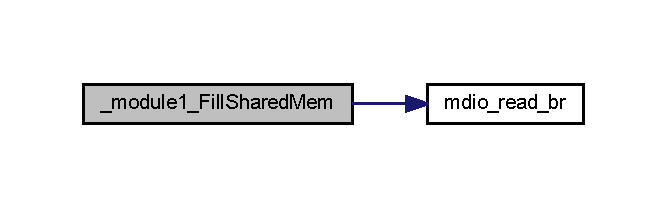
\includegraphics[width=320pt]{module_one_read_eth_phy_8c_aac64c1f68d24bc5a269cd0c8b2d6a483_cgraph}
\end{center}
\end{figure}
\mbox{\Hypertarget{module_one_read_eth_phy_8c_a7fa5a1147c84061bd511408e7fc92e77}\label{module_one_read_eth_phy_8c_a7fa5a1147c84061bd511408e7fc92e77}} 
\index{module\+One\+Read\+Eth\+Phy.\+c@{module\+One\+Read\+Eth\+Phy.\+c}!\+\_\+module1\+\_\+get\+Error\+Time@{\+\_\+module1\+\_\+get\+Error\+Time}}
\index{\+\_\+module1\+\_\+get\+Error\+Time@{\+\_\+module1\+\_\+get\+Error\+Time}!module\+One\+Read\+Eth\+Phy.\+c@{module\+One\+Read\+Eth\+Phy.\+c}}
\subsubsection{\texorpdfstring{\+\_\+module1\+\_\+get\+Error\+Time()}{\_module1\_getErrorTime()}}
{\footnotesize\ttfamily L\+O\+C\+AL void \+\_\+module1\+\_\+get\+Error\+Time (\begin{DoxyParamCaption}\item[{struct tm const $\ast$}]{time\+\_\+info,  }\item[{uint8\+\_\+t}]{pos }\end{DoxyParamCaption})}



Function that gets time of error. 


\begin{DoxyParams}{Parameters}
{\em time\+\_\+info} & Struct tm with current processor time \\
\hline
{\em pos} & Position of error in errors\+\_\+array struct  S\+T\+A\+V1 11 Library functions. \\
\hline
\end{DoxyParams}
\mbox{\Hypertarget{module_one_read_eth_phy_8c_ad3d33414850bbc909d7abadd9374d260}\label{module_one_read_eth_phy_8c_ad3d33414850bbc909d7abadd9374d260}} 
\index{module\+One\+Read\+Eth\+Phy.\+c@{module\+One\+Read\+Eth\+Phy.\+c}!\+\_\+module1\+\_\+\+Read\+Chip\+Registers@{\+\_\+module1\+\_\+\+Read\+Chip\+Registers}}
\index{\+\_\+module1\+\_\+\+Read\+Chip\+Registers@{\+\_\+module1\+\_\+\+Read\+Chip\+Registers}!module\+One\+Read\+Eth\+Phy.\+c@{module\+One\+Read\+Eth\+Phy.\+c}}
\subsubsection{\texorpdfstring{\+\_\+module1\+\_\+\+Read\+Chip\+Registers()}{\_module1\_ReadChipRegisters()}}
{\footnotesize\ttfamily L\+O\+C\+AL void \+\_\+module1\+\_\+\+Read\+Chip\+Registers (\begin{DoxyParamCaption}\item[{void}]{ }\end{DoxyParamCaption})}



Function that reads registers and fill diag data structure  S\+T\+A\+V1 10 Loading data in msgQ struct. 

Here is the call graph for this function\+:\nopagebreak
\begin{figure}[H]
\begin{center}
\leavevmode
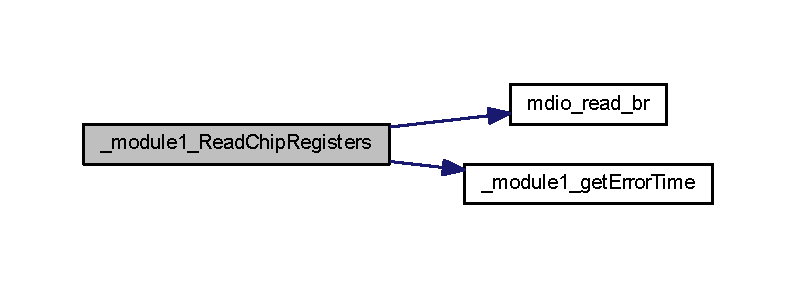
\includegraphics[width=350pt]{module_one_read_eth_phy_8c_ad3d33414850bbc909d7abadd9374d260_cgraph}
\end{center}
\end{figure}
\mbox{\Hypertarget{module_one_read_eth_phy_8c_a259f47509afd861ed65a4c74e1654da7}\label{module_one_read_eth_phy_8c_a259f47509afd861ed65a4c74e1654da7}} 
\index{module\+One\+Read\+Eth\+Phy.\+c@{module\+One\+Read\+Eth\+Phy.\+c}!\+\_\+module1\+\_\+sh\+Mem\+\_\+\+Alloc@{\+\_\+module1\+\_\+sh\+Mem\+\_\+\+Alloc}}
\index{\+\_\+module1\+\_\+sh\+Mem\+\_\+\+Alloc@{\+\_\+module1\+\_\+sh\+Mem\+\_\+\+Alloc}!module\+One\+Read\+Eth\+Phy.\+c@{module\+One\+Read\+Eth\+Phy.\+c}}
\subsubsection{\texorpdfstring{\+\_\+module1\+\_\+sh\+Mem\+\_\+\+Alloc()}{\_module1\_shMem\_Alloc()}}
{\footnotesize\ttfamily L\+O\+C\+AL void $\ast$ \+\_\+module1\+\_\+sh\+Mem\+\_\+\+Alloc (\begin{DoxyParamCaption}\item[{const char $\ast$}]{fname,  }\item[{size\+\_\+t}]{size }\end{DoxyParamCaption})}



This function opens shared memory and allocates it. 


\begin{DoxyParams}{Parameters}
{\em fname} & Shared memory name \\
\hline
{\em size} & Shared memory size \\
\hline
\end{DoxyParams}
\begin{DoxyReturn}{Returns}
Pointer to allocated shared memory 
\end{DoxyReturn}
\mbox{\Hypertarget{module_one_read_eth_phy_8c_a4d2f336ff3392dcabf55d8aad27395c2}\label{module_one_read_eth_phy_8c_a4d2f336ff3392dcabf55d8aad27395c2}} 
\index{module\+One\+Read\+Eth\+Phy.\+c@{module\+One\+Read\+Eth\+Phy.\+c}!\+\_\+shared\+Mem\+Alloc@{\+\_\+shared\+Mem\+Alloc}}
\index{\+\_\+shared\+Mem\+Alloc@{\+\_\+shared\+Mem\+Alloc}!module\+One\+Read\+Eth\+Phy.\+c@{module\+One\+Read\+Eth\+Phy.\+c}}
\subsubsection{\texorpdfstring{\+\_\+shared\+Mem\+Alloc()}{\_sharedMemAlloc()}}
{\footnotesize\ttfamily L\+O\+C\+AL S\+T\+A\+T\+US \+\_\+shared\+Mem\+Alloc (\begin{DoxyParamCaption}\item[{void}]{ }\end{DoxyParamCaption})}



This function takes pointer to allocated shared memory. 

\begin{DoxyReturn}{Returns}
OK if successful, E\+R\+R\+OR otherwise  E\+R\+R\+OR if opening shared memory failed 
\end{DoxyReturn}
Here is the call graph for this function\+:\nopagebreak
\begin{figure}[H]
\begin{center}
\leavevmode
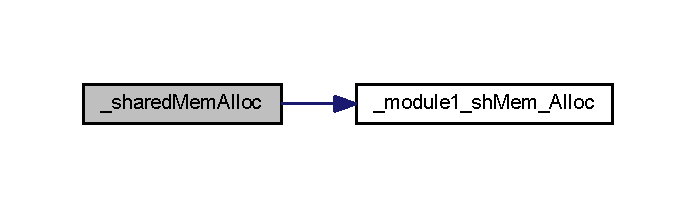
\includegraphics[width=334pt]{module_one_read_eth_phy_8c_a4d2f336ff3392dcabf55d8aad27395c2_cgraph}
\end{center}
\end{figure}
\mbox{\Hypertarget{module_one_read_eth_phy_8c_a47c6c4d64e604e8e2c2e17b23a63e053}\label{module_one_read_eth_phy_8c_a47c6c4d64e604e8e2c2e17b23a63e053}} 
\index{module\+One\+Read\+Eth\+Phy.\+c@{module\+One\+Read\+Eth\+Phy.\+c}!mdio\+\_\+read\+\_\+br@{mdio\+\_\+read\+\_\+br}}
\index{mdio\+\_\+read\+\_\+br@{mdio\+\_\+read\+\_\+br}!module\+One\+Read\+Eth\+Phy.\+c@{module\+One\+Read\+Eth\+Phy.\+c}}
\subsubsection{\texorpdfstring{mdio\+\_\+read\+\_\+br()}{mdio\_read\_br()}}
{\footnotesize\ttfamily uint32\+\_\+t mdio\+\_\+read\+\_\+br (\begin{DoxyParamCaption}\item[{uint32\+\_\+t}]{reg\+Number }\end{DoxyParamCaption})}



This function reads T\+J\+A1100 address register. 


\begin{DoxyParams}{Parameters}
{\em reg\+Number} & Number of desired Broad\+R\+Reach register\\
\hline
\end{DoxyParams}
\begin{DoxyReturn}{Returns}
data\+Read Data read from register 
\end{DoxyReturn}

\begin{DoxyRetVals}{Return values}
{\em 0} & Reading from register failed \\
\hline
{\em phy\+Gmii\+Data} & Reading from register success \\
\hline
\end{DoxyRetVals}
\mbox{\Hypertarget{module_one_read_eth_phy_8c_a50ee291d74529a7a8e2ea86f6aa2f2bf}\label{module_one_read_eth_phy_8c_a50ee291d74529a7a8e2ea86f6aa2f2bf}} 
\index{module\+One\+Read\+Eth\+Phy.\+c@{module\+One\+Read\+Eth\+Phy.\+c}!mdio\+\_\+write\+\_\+br@{mdio\+\_\+write\+\_\+br}}
\index{mdio\+\_\+write\+\_\+br@{mdio\+\_\+write\+\_\+br}!module\+One\+Read\+Eth\+Phy.\+c@{module\+One\+Read\+Eth\+Phy.\+c}}
\subsubsection{\texorpdfstring{mdio\+\_\+write\+\_\+br()}{mdio\_write\_br()}}
{\footnotesize\ttfamily void mdio\+\_\+write\+\_\+br (\begin{DoxyParamCaption}\item[{uint32\+\_\+t}]{reg\+Number,  }\item[{uint16\+\_\+t}]{data\+Write }\end{DoxyParamCaption})}



This function writes data to T\+J\+A1100 address register. 


\begin{DoxyParams}{Parameters}
{\em reg\+Number} & Number of Broad\+R\+Reach register \\
\hline
{\em data\+Write} & Data to be written \\
\hline
\end{DoxyParams}
\mbox{\Hypertarget{module_one_read_eth_phy_8c_ab4a7c038fb29787895e96b7521eede34}\label{module_one_read_eth_phy_8c_ab4a7c038fb29787895e96b7521eede34}} 
\index{module\+One\+Read\+Eth\+Phy.\+c@{module\+One\+Read\+Eth\+Phy.\+c}!module1\+\_\+\+Read\+Chip\+Registers\+Task@{module1\+\_\+\+Read\+Chip\+Registers\+Task}}
\index{module1\+\_\+\+Read\+Chip\+Registers\+Task@{module1\+\_\+\+Read\+Chip\+Registers\+Task}!module\+One\+Read\+Eth\+Phy.\+c@{module\+One\+Read\+Eth\+Phy.\+c}}
\subsubsection{\texorpdfstring{module1\+\_\+\+Read\+Chip\+Registers\+Task()}{module1\_ReadChipRegistersTask()}}
{\footnotesize\ttfamily void module1\+\_\+\+Read\+Chip\+Registers\+Task (\begin{DoxyParamCaption}\item[{void}]{ }\end{DoxyParamCaption})}



This is task function for module1\+Read\+Chip\+Registers() used for reading T\+J\+A1100 registers and sending data to diag\+MsgQ via diag\+\_\+data\+\_\+struct. 

Here is the call graph for this function\+:\nopagebreak
\begin{figure}[H]
\begin{center}
\leavevmode
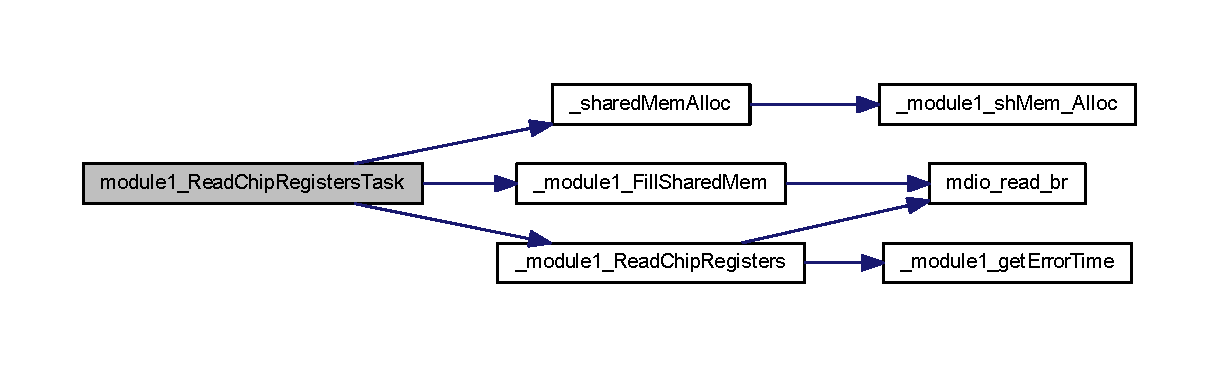
\includegraphics[width=350pt]{module_one_read_eth_phy_8c_ab4a7c038fb29787895e96b7521eede34_cgraph}
\end{center}
\end{figure}


\subsection{Variable Documentation}
\mbox{\Hypertarget{module_one_read_eth_phy_8c_a48ce9a0018fd97bde8d9f92965f22267}\label{module_one_read_eth_phy_8c_a48ce9a0018fd97bde8d9f92965f22267}} 
\index{module\+One\+Read\+Eth\+Phy.\+c@{module\+One\+Read\+Eth\+Phy.\+c}!\+\_\+delete\+\_\+cnt@{\+\_\+delete\+\_\+cnt}}
\index{\+\_\+delete\+\_\+cnt@{\+\_\+delete\+\_\+cnt}!module\+One\+Read\+Eth\+Phy.\+c@{module\+One\+Read\+Eth\+Phy.\+c}}
\subsubsection{\texorpdfstring{\+\_\+delete\+\_\+cnt}{\_delete\_cnt}}
{\footnotesize\ttfamily L\+O\+C\+AL uint8\+\_\+t \+\_\+delete\+\_\+cnt = 0U}

\mbox{\Hypertarget{module_one_read_eth_phy_8c_ab6154d17a17c7941b815a06de15f8c54}\label{module_one_read_eth_phy_8c_ab6154d17a17c7941b815a06de15f8c54}} 
\index{module\+One\+Read\+Eth\+Phy.\+c@{module\+One\+Read\+Eth\+Phy.\+c}!\+\_\+diag\+\_\+data\+\_\+struct@{\+\_\+diag\+\_\+data\+\_\+struct}}
\index{\+\_\+diag\+\_\+data\+\_\+struct@{\+\_\+diag\+\_\+data\+\_\+struct}!module\+One\+Read\+Eth\+Phy.\+c@{module\+One\+Read\+Eth\+Phy.\+c}}
\subsubsection{\texorpdfstring{\+\_\+diag\+\_\+data\+\_\+struct}{\_diag\_data\_struct}}
{\footnotesize\ttfamily \mbox{\hyperlink{__module3_8h_a58c449f6052675fb4288c20122741cb8}{s\+\_\+\+D\+I\+A\+G\+\_\+\+D\+A\+TA}} \+\_\+diag\+\_\+data\+\_\+struct}

\mbox{\Hypertarget{module_one_read_eth_phy_8c_ac83d0a83ca252211302d67059d2b781e}\label{module_one_read_eth_phy_8c_ac83d0a83ca252211302d67059d2b781e}} 
\index{module\+One\+Read\+Eth\+Phy.\+c@{module\+One\+Read\+Eth\+Phy.\+c}!\+\_\+diag\+\_\+shm\+\_\+ptr@{\+\_\+diag\+\_\+shm\+\_\+ptr}}
\index{\+\_\+diag\+\_\+shm\+\_\+ptr@{\+\_\+diag\+\_\+shm\+\_\+ptr}!module\+One\+Read\+Eth\+Phy.\+c@{module\+One\+Read\+Eth\+Phy.\+c}}
\subsubsection{\texorpdfstring{\+\_\+diag\+\_\+shm\+\_\+ptr}{\_diag\_shm\_ptr}}
{\footnotesize\ttfamily \mbox{\hyperlink{__module3_8h_a1f542cc6438c66026963a340365d442a}{s\+\_\+\+D\+I\+A\+G\+\_\+\+S\+H\+M\+\_\+\+D\+A\+TA}}$\ast$ \+\_\+diag\+\_\+shm\+\_\+ptr}


\hypertarget{module_one_read_eth_phy_8h}{}\section{module\+One\+Read\+Eth\+Phy.\+h File Reference}
\label{module_one_read_eth_phy_8h}\index{module\+One\+Read\+Eth\+Phy.\+h@{module\+One\+Read\+Eth\+Phy.\+h}}
This graph shows which files directly or indirectly include this file\+:
\nopagebreak
\begin{figure}[H]
\begin{center}
\leavevmode
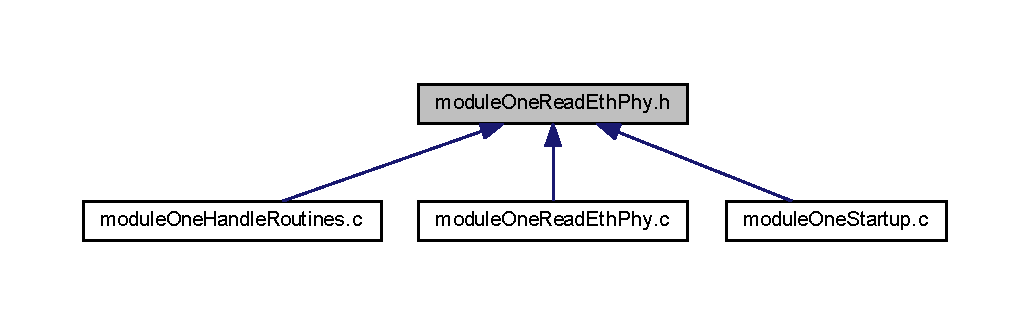
\includegraphics[width=350pt]{module_one_read_eth_phy_8h__dep__incl}
\end{center}
\end{figure}
\subsection*{Classes}
\begin{DoxyCompactItemize}
\item 
struct \mbox{\hyperlink{structerror_struct}{error\+Struct}}
\item 
struct \mbox{\hyperlink{structdiagnostic_data_msg_q}{diagnostic\+Data\+MsgQ}}
\item 
struct \mbox{\hyperlink{structdiagnostic_data_sh_m}{diagnostic\+Data\+ShM}}
\end{DoxyCompactItemize}
\subsection*{Macros}
\begin{DoxyCompactItemize}
\item 
\#define \mbox{\hyperlink{module_one_read_eth_phy_8h_a555f824010392043fd8a9384d1ec3b15}{H\+O\+S\+T\+\_\+\+BR}}~\char`\"{}fd53\+:7cb8\+:383\+:2\+::4f\char`\"{}
\item 
\#define \mbox{\hyperlink{module_one_read_eth_phy_8h_ae72fb1d3362993b4cbbe6d79fd424c6e}{M\+A\+C\+\_\+\+BR}}~\char`\"{}8a\+:23\+:fe\+:0x00\+:0x00\+:02\char`\"{}
\item 
\#define \mbox{\hyperlink{module_one_read_eth_phy_8h_a306abfd62ab935890f8c4a226b7ce350}{P\+C\+\_\+\+I\+P\+V6}}~\char`\"{}fd53\+:7cb8\+:383\+:3\+::73\char`\"{}
\item 
\#define \mbox{\hyperlink{module_one_read_eth_phy_8h_ad89c5a76e69b781c64de110635a95d1d}{S\+H\+\_\+\+M\+E\+M\+\_\+\+N\+A\+ME}}~\char`\"{}/sh\+Mem\+Module1to2\char`\"{}
\item 
\#define \mbox{\hyperlink{module_one_read_eth_phy_8h_a64d438edbdcb3832dd5a4dc0f261d5dd}{G\+M\+I\+I\+A\+D\+D\+R\+E\+SS}}~((uint32\+\_\+t) 0x\+F\+F702010\+U)
\item 
\#define \mbox{\hyperlink{module_one_read_eth_phy_8h_a7fe6fa7743bd33dd5be21796001ccc55}{G\+M\+I\+I\+D\+A\+TA}}~((uint32\+\_\+t) 0x\+F\+F702014\+U)
\item 
\#define \mbox{\hyperlink{module_one_read_eth_phy_8h_ae72e1fb9c55d5804aec7e9a342db7b34}{C\+L\+E\+A\+R\+\_\+\+M\+A\+SK}}~((uint32\+\_\+t) 0x\+F\+F\+F\+F0000\+U)
\item 
\#define \mbox{\hyperlink{module_one_read_eth_phy_8h_a8150b21f39fdf77abaa90e4a13aacaaa}{S\+E\+T\+\_\+\+R\+E\+A\+D\+\_\+\+M\+A\+SK}}~((uint32\+\_\+t) 0x00000001\+U)
\item 
\#define \mbox{\hyperlink{module_one_read_eth_phy_8h_a7a7f4a7b0a9f49e347105cd8acc3efa4}{S\+E\+T\+\_\+\+W\+R\+I\+T\+E\+\_\+\+M\+A\+SK}}~((uint32\+\_\+t) 0x00000003\+U)
\item 
\#define \mbox{\hyperlink{module_one_read_eth_phy_8h_a7e9eda34f27d379d599f1dc4cd837ff3}{B\+U\+S\+Y\+\_\+\+B\+IT}}~((uint32\+\_\+t) 0x1\+U)
\item 
\#define \mbox{\hyperlink{module_one_read_eth_phy_8h_a936d080dc46f388c9449a7bf26ce7c40}{B\+I\+T\+\_\+\+O\+F\+F\+S\+ET}}~((uint8\+\_\+t) 6\+U)
\item 
\#define \mbox{\hyperlink{module_one_read_eth_phy_8h_aa24597a54a085c6c2c33b64138f09eff}{M\+A\+X\+\_\+\+M\+SG}}~((uint8\+\_\+t) 2\+U)
\item 
\#define \mbox{\hyperlink{module_one_read_eth_phy_8h_a51d90ea93d4b55e086cb490f7478e684}{M\+A\+X\+\_\+\+M\+S\+G\+\_\+\+L\+EN}}~((uint8\+\_\+t) 8\+U)
\item 
\#define \mbox{\hyperlink{module_one_read_eth_phy_8h_a5c6f13cd61f3d2e005687bbe43cd212c}{L\+I\+N\+K\+\_\+\+S\+T\+A\+T\+U\+S\+\_\+\+M\+A\+SK}}~((uint32\+\_\+t) 0x0004\+U)
\item 
\#define \mbox{\hyperlink{module_one_read_eth_phy_8h_a7510b53d2c374d1846f5b4af999548a0}{L\+I\+N\+K\+\_\+\+C\+O\+N\+T\+R\+O\+L\+\_\+\+M\+A\+SK}}~((uint32\+\_\+t) 0x8000\+U)
\item 
\#define \mbox{\hyperlink{module_one_read_eth_phy_8h_a2b5d1b8c5aa42d1b5f0d8a5adb572abe}{P\+O\+W\+E\+R\+\_\+\+M\+O\+D\+E\+\_\+\+M\+A\+SK}}~((uint32\+\_\+t) 0x7800\+U)
\item 
\#define \mbox{\hyperlink{module_one_read_eth_phy_8h_a9bc69d8279625eb1da0625adbca5942c}{L\+O\+O\+P\+B\+A\+C\+K\+\_\+\+M\+O\+D\+E\+\_\+\+M\+A\+SK}}~((uint32\+\_\+t) 0x0018\+U)
\item 
\#define \mbox{\hyperlink{module_one_read_eth_phy_8h_ac0485e3a69e3c935a4feae824a5f6fcb}{P\+H\+Y\+\_\+\+F\+A\+I\+L\+\_\+\+M\+A\+SK}}~((uint32\+\_\+t) 0x0800\+U)
\item 
\#define \mbox{\hyperlink{module_one_read_eth_phy_8h_a2b472fdbbf78dae0a12b301125591ef2}{W\+A\+K\+E\+U\+P\+\_\+\+M\+A\+SK}}~((uint32\+\_\+t) 0x4000\+U)
\item 
\#define \mbox{\hyperlink{module_one_read_eth_phy_8h_aafe6c908d5d05c93bf7cc01bdf8689e3}{L\+I\+N\+K\+\_\+\+S\+T\+A\+T\+U\+S\+\_\+\+F\+A\+I\+L\+\_\+\+M\+A\+SK}}~((uint32\+\_\+t) 0x0400\+U)
\item 
\#define \mbox{\hyperlink{module_one_read_eth_phy_8h_a45f2e383f7d5d29437c8c3d9db9b37db}{L\+I\+N\+K\+\_\+\+S\+T\+A\+T\+U\+S\+\_\+\+U\+P\+\_\+\+M\+A\+SK}}~((uint32\+\_\+t) 0x0200\+U)
\item 
\#define \mbox{\hyperlink{module_one_read_eth_phy_8h_a061337cd00b354e7cd796d4332a39f40}{L\+I\+N\+K\+\_\+\+U\+P\+\_\+\+M\+A\+SK}}~((uint32\+\_\+t) 0x8000\+U)
\item 
\#define \mbox{\hyperlink{module_one_read_eth_phy_8h_a04599ec8f5078977a78cd558661d6caf}{T\+X\+\_\+\+M\+O\+D\+E\+\_\+\+M\+A\+SK}}~((uint32\+\_\+t) 0x6000\+U)
\item 
\#define \mbox{\hyperlink{module_one_read_eth_phy_8h_a9a4931e5e2ee2b0ee77efac783e3af57}{L\+O\+C\+\_\+\+R\+C\+V\+R\+\_\+\+M\+A\+SK}}~((uint32\+\_\+t) 0x1000\+U)
\item 
\#define \mbox{\hyperlink{module_one_read_eth_phy_8h_a185405e27cd55f75f217d0bc07fdc2c4}{R\+E\+M\+\_\+\+R\+C\+V\+R\+\_\+\+M\+A\+SK}}~((uint32\+\_\+t) 0x0800\+U)
\item 
\#define \mbox{\hyperlink{module_one_read_eth_phy_8h_aa8de95c611d52d7fd61de6a0563e41ce}{J\+A\+B\+B\+E\+R\+\_\+\+D\+E\+T\+E\+C\+T\+\_\+\+M\+A\+SK}}~((uint32\+\_\+t) 0x0002\+U)
\item 
\#define \mbox{\hyperlink{module_one_read_eth_phy_8h_a7b0d046cc887a20e50184f6d9ed89ad9}{P\+H\+Y\+\_\+\+I\+D\+\_\+\+R\+E\+G2\+\_\+\+M\+A\+SK}}~((uint32\+\_\+t) 0x\+F\+C00\+U)
\item 
\#define \mbox{\hyperlink{module_one_read_eth_phy_8h_a06f085911ecd47aa9a10517aeba09c2a}{T\+Y\+P\+E\+\_\+\+N\+O\+\_\+\+M\+A\+SK}}~((uint32\+\_\+t) 0x03\+F0\+U)
\item 
\#define \mbox{\hyperlink{module_one_read_eth_phy_8h_a914aa7070c5c3f0ca2b73615a1622e15}{R\+E\+V\+I\+S\+I\+O\+N\+\_\+\+N\+O\+\_\+\+M\+A\+SK}}~((uint32\+\_\+t) 0x000\+F\+U)
\item 
\#define \mbox{\hyperlink{module_one_read_eth_phy_8h_a950b5294c49f552f3634cf8ed2c30db6}{P\+H\+Y\+\_\+\+I\+D\+\_\+\+R\+E\+G3\+\_\+\+M\+A\+SK}}~((uint32\+\_\+t) 0x00\+F\+F\+U)
\item 
\#define \mbox{\hyperlink{module_one_read_eth_phy_8h_a61aa6e34efda022931edbba16af52940}{I\+N\+T\+\_\+\+S\+T\+A\+T\+U\+S\+\_\+\+M\+A\+SK}}~((uint32\+\_\+t) 0x8000\+U)
\item 
\#define \mbox{\hyperlink{module_one_read_eth_phy_8h_a530f11a96e508d171d28564c8dc20942}{N\+U\+L\+L\+\_\+\+P\+TR}}~(void $\ast$) (0)
\item 
\#define \mbox{\hyperlink{module_one_read_eth_phy_8h_a146d7dedfdc15b1c2395679adb8d8ed4}{T\+A\+S\+K\+\_\+\+D\+E\+L\+A\+Y\+\_\+250\+MS}}~(uint32\+\_\+t) (25\+U)
\item 
\#define \mbox{\hyperlink{module_one_read_eth_phy_8h_a1e27817ee436cbdeba83c2a35fe9cd44}{T\+A\+S\+K\+\_\+\+D\+E\+L\+A\+Y\+\_\+1000\+MS}}~(uint32\+\_\+t) (100\+U)
\item 
\#define \mbox{\hyperlink{module_one_read_eth_phy_8h_a541dee5b5d73b673359a46ad53ff9527}{B\+A\+S\+I\+C\+\_\+\+S\+T\+A\+T\+U\+S\+\_\+\+R\+E\+G\+I\+S\+T\+ER}}~((uint32\+\_\+t) (0x1))
\item 
\#define \mbox{\hyperlink{module_one_read_eth_phy_8h_a92d5ac48c7f09632af3039f2e787cb3b}{P\+H\+Y\+\_\+\+I\+D\+\_\+\+R\+E\+G\+I\+S\+T\+E\+R\+\_\+1}}~((uint32\+\_\+t) (0x2))
\item 
\#define \mbox{\hyperlink{module_one_read_eth_phy_8h_ae0f83d5f7de36094abd838fafe92cc8d}{P\+H\+Y\+\_\+\+I\+D\+\_\+\+R\+E\+G\+I\+S\+T\+E\+R\+\_\+2}}~((uint32\+\_\+t) (0x3))
\item 
\#define \mbox{\hyperlink{module_one_read_eth_phy_8h_a18c09617ca430f3dab9eebbe16dbf4f1}{P\+H\+Y\+\_\+\+I\+D\+\_\+\+R\+E\+G\+I\+S\+T\+E\+R\+\_\+3}}~((uint32\+\_\+t) (0x10))
\item 
\#define \mbox{\hyperlink{module_one_read_eth_phy_8h_ade5100260c2704fcf09efb04195ab30d}{G\+E\+N\+E\+R\+A\+L\+\_\+\+S\+T\+A\+T\+U\+S\+\_\+\+R\+E\+G\+I\+S\+T\+ER}}~((uint32\+\_\+t) (0x18))
\item 
\#define \mbox{\hyperlink{module_one_read_eth_phy_8h_affbfbb29eccba558f22033239167d870}{E\+X\+T\+E\+N\+D\+E\+D\+\_\+\+C\+O\+N\+T\+R\+O\+L\+\_\+\+R\+E\+G\+I\+S\+T\+ER}}~((uint32\+\_\+t) (0x11))
\item 
\#define \mbox{\hyperlink{module_one_read_eth_phy_8h_a55dac77bf62fc543e1f6c3f8e97b98d4}{I\+N\+T\+E\+R\+R\+U\+P\+T\+\_\+\+S\+O\+U\+R\+C\+E\+\_\+\+R\+E\+G\+I\+S\+T\+ER}}~((uint32\+\_\+t) (0x15))
\item 
\#define \mbox{\hyperlink{module_one_read_eth_phy_8h_a7b3231c45827132795a985df98b30788}{C\+O\+M\+M\+U\+N\+I\+C\+A\+T\+I\+O\+N\+\_\+\+S\+T\+A\+T\+U\+S\+\_\+\+R\+E\+G\+I\+S\+T\+ER}}~((uint32\+\_\+t) (0x17))
\item 
\#define \mbox{\hyperlink{module_one_read_eth_phy_8h_ad6a5f0870f87a830a9281a48c20d1967}{C\+O\+N\+F\+I\+G\+U\+R\+A\+T\+I\+O\+N\+\_\+\+R\+E\+G\+I\+S\+T\+E\+R\+\_\+1}}~((uint32\+\_\+t) (0x12))
\item 
\#define \mbox{\hyperlink{module_one_read_eth_phy_8h_ab9a10f48a2538ff4e5d537c4d8d41a70}{M\+A\+X\+\_\+\+C\+NT}}~(255\+U)
\end{DoxyCompactItemize}
\subsection*{Typedefs}
\begin{DoxyCompactItemize}
\item 
typedef struct \mbox{\hyperlink{structerror_struct}{error\+Struct}} \mbox{\hyperlink{module_one_read_eth_phy_8h_a20a1de38f8a31b563f5185bf73d836b0}{s\+\_\+\+E\+R\+R\+O\+RS}}
\item 
typedef struct \mbox{\hyperlink{structdiagnostic_data_msg_q}{diagnostic\+Data\+MsgQ}} \mbox{\hyperlink{module_one_read_eth_phy_8h_a58c449f6052675fb4288c20122741cb8}{s\+\_\+\+D\+I\+A\+G\+\_\+\+D\+A\+TA}}
\item 
typedef struct \mbox{\hyperlink{structdiagnostic_data_sh_m}{diagnostic\+Data\+ShM}} \mbox{\hyperlink{module_one_read_eth_phy_8h_a1f542cc6438c66026963a340365d442a}{s\+\_\+\+D\+I\+A\+G\+\_\+\+S\+H\+M\+\_\+\+D\+A\+TA}}
\end{DoxyCompactItemize}
\subsection*{Functions}
\begin{DoxyCompactItemize}
\item 
uint32\+\_\+t \mbox{\hyperlink{module_one_read_eth_phy_8h_a47c6c4d64e604e8e2c2e17b23a63e053}{mdio\+\_\+read\+\_\+br}} (uint32\+\_\+t reg\+Number)
\begin{DoxyCompactList}\small\item\em This function reads T\+J\+A1100 address register. \end{DoxyCompactList}\item 
void \mbox{\hyperlink{module_one_read_eth_phy_8h_a50ee291d74529a7a8e2ea86f6aa2f2bf}{mdio\+\_\+write\+\_\+br}} (uint32\+\_\+t reg\+Number, uint16\+\_\+t data\+Write)
\begin{DoxyCompactList}\small\item\em This function writes data to T\+J\+A1100 address register. \end{DoxyCompactList}\item 
void \mbox{\hyperlink{module_one_read_eth_phy_8h_ab4a7c038fb29787895e96b7521eede34}{module1\+\_\+\+Read\+Chip\+Registers\+Task}} (void)
\begin{DoxyCompactList}\small\item\em This is task function for module1\+Read\+Chip\+Registers() used for reading T\+J\+A1100 registers and sending data to diag\+MsgQ via diag\+\_\+data\+\_\+struct. \end{DoxyCompactList}\end{DoxyCompactItemize}
\subsection*{Variables}
\begin{DoxyCompactItemize}
\item 
M\+S\+G\+\_\+\+Q\+\_\+\+ID \mbox{\hyperlink{module_one_read_eth_phy_8h_a6ae24b34485eed59336d11223d848886}{diag\+Msg\+Q\+Id}}
\item 
volatile uint32\+\_\+t $\ast$ \mbox{\hyperlink{module_one_read_eth_phy_8h_a30a534f860e9976401cc923843ef91c7}{phy\+Gmii\+Address}}
\item 
volatile uint32\+\_\+t $\ast$ \mbox{\hyperlink{module_one_read_eth_phy_8h_a552978b3e139f218293760bfa8b8dfaa}{phy\+Gmii\+Data}}
\item 
\mbox{\hyperlink{module_one_read_eth_phy_8h_a58c449f6052675fb4288c20122741cb8}{s\+\_\+\+D\+I\+A\+G\+\_\+\+D\+A\+TA}} \mbox{\hyperlink{module_one_read_eth_phy_8h_ab6154d17a17c7941b815a06de15f8c54}{\+\_\+diag\+\_\+data\+\_\+struct}}
\item 
\mbox{\hyperlink{module_one_read_eth_phy_8h_a1f542cc6438c66026963a340365d442a}{s\+\_\+\+D\+I\+A\+G\+\_\+\+S\+H\+M\+\_\+\+D\+A\+TA}} $\ast$ \mbox{\hyperlink{module_one_read_eth_phy_8h_ac83d0a83ca252211302d67059d2b781e}{\+\_\+diag\+\_\+shm\+\_\+ptr}}
\end{DoxyCompactItemize}


\subsection{Macro Definition Documentation}
\mbox{\Hypertarget{module_one_read_eth_phy_8h_a541dee5b5d73b673359a46ad53ff9527}\label{module_one_read_eth_phy_8h_a541dee5b5d73b673359a46ad53ff9527}} 
\index{module\+One\+Read\+Eth\+Phy.\+h@{module\+One\+Read\+Eth\+Phy.\+h}!B\+A\+S\+I\+C\+\_\+\+S\+T\+A\+T\+U\+S\+\_\+\+R\+E\+G\+I\+S\+T\+ER@{B\+A\+S\+I\+C\+\_\+\+S\+T\+A\+T\+U\+S\+\_\+\+R\+E\+G\+I\+S\+T\+ER}}
\index{B\+A\+S\+I\+C\+\_\+\+S\+T\+A\+T\+U\+S\+\_\+\+R\+E\+G\+I\+S\+T\+ER@{B\+A\+S\+I\+C\+\_\+\+S\+T\+A\+T\+U\+S\+\_\+\+R\+E\+G\+I\+S\+T\+ER}!module\+One\+Read\+Eth\+Phy.\+h@{module\+One\+Read\+Eth\+Phy.\+h}}
\subsubsection{\texorpdfstring{B\+A\+S\+I\+C\+\_\+\+S\+T\+A\+T\+U\+S\+\_\+\+R\+E\+G\+I\+S\+T\+ER}{BASIC\_STATUS\_REGISTER}}
{\footnotesize\ttfamily \#define B\+A\+S\+I\+C\+\_\+\+S\+T\+A\+T\+U\+S\+\_\+\+R\+E\+G\+I\+S\+T\+ER~((uint32\+\_\+t) (0x1))}

\mbox{\Hypertarget{module_one_read_eth_phy_8h_a936d080dc46f388c9449a7bf26ce7c40}\label{module_one_read_eth_phy_8h_a936d080dc46f388c9449a7bf26ce7c40}} 
\index{module\+One\+Read\+Eth\+Phy.\+h@{module\+One\+Read\+Eth\+Phy.\+h}!B\+I\+T\+\_\+\+O\+F\+F\+S\+ET@{B\+I\+T\+\_\+\+O\+F\+F\+S\+ET}}
\index{B\+I\+T\+\_\+\+O\+F\+F\+S\+ET@{B\+I\+T\+\_\+\+O\+F\+F\+S\+ET}!module\+One\+Read\+Eth\+Phy.\+h@{module\+One\+Read\+Eth\+Phy.\+h}}
\subsubsection{\texorpdfstring{B\+I\+T\+\_\+\+O\+F\+F\+S\+ET}{BIT\_OFFSET}}
{\footnotesize\ttfamily \#define B\+I\+T\+\_\+\+O\+F\+F\+S\+ET~((uint8\+\_\+t) 6\+U)}

\mbox{\Hypertarget{module_one_read_eth_phy_8h_a7e9eda34f27d379d599f1dc4cd837ff3}\label{module_one_read_eth_phy_8h_a7e9eda34f27d379d599f1dc4cd837ff3}} 
\index{module\+One\+Read\+Eth\+Phy.\+h@{module\+One\+Read\+Eth\+Phy.\+h}!B\+U\+S\+Y\+\_\+\+B\+IT@{B\+U\+S\+Y\+\_\+\+B\+IT}}
\index{B\+U\+S\+Y\+\_\+\+B\+IT@{B\+U\+S\+Y\+\_\+\+B\+IT}!module\+One\+Read\+Eth\+Phy.\+h@{module\+One\+Read\+Eth\+Phy.\+h}}
\subsubsection{\texorpdfstring{B\+U\+S\+Y\+\_\+\+B\+IT}{BUSY\_BIT}}
{\footnotesize\ttfamily \#define B\+U\+S\+Y\+\_\+\+B\+IT~((uint32\+\_\+t) 0x1\+U)}

\mbox{\Hypertarget{module_one_read_eth_phy_8h_ae72e1fb9c55d5804aec7e9a342db7b34}\label{module_one_read_eth_phy_8h_ae72e1fb9c55d5804aec7e9a342db7b34}} 
\index{module\+One\+Read\+Eth\+Phy.\+h@{module\+One\+Read\+Eth\+Phy.\+h}!C\+L\+E\+A\+R\+\_\+\+M\+A\+SK@{C\+L\+E\+A\+R\+\_\+\+M\+A\+SK}}
\index{C\+L\+E\+A\+R\+\_\+\+M\+A\+SK@{C\+L\+E\+A\+R\+\_\+\+M\+A\+SK}!module\+One\+Read\+Eth\+Phy.\+h@{module\+One\+Read\+Eth\+Phy.\+h}}
\subsubsection{\texorpdfstring{C\+L\+E\+A\+R\+\_\+\+M\+A\+SK}{CLEAR\_MASK}}
{\footnotesize\ttfamily \#define C\+L\+E\+A\+R\+\_\+\+M\+A\+SK~((uint32\+\_\+t) 0x\+F\+F\+F\+F0000\+U)}

\mbox{\Hypertarget{module_one_read_eth_phy_8h_a7b3231c45827132795a985df98b30788}\label{module_one_read_eth_phy_8h_a7b3231c45827132795a985df98b30788}} 
\index{module\+One\+Read\+Eth\+Phy.\+h@{module\+One\+Read\+Eth\+Phy.\+h}!C\+O\+M\+M\+U\+N\+I\+C\+A\+T\+I\+O\+N\+\_\+\+S\+T\+A\+T\+U\+S\+\_\+\+R\+E\+G\+I\+S\+T\+ER@{C\+O\+M\+M\+U\+N\+I\+C\+A\+T\+I\+O\+N\+\_\+\+S\+T\+A\+T\+U\+S\+\_\+\+R\+E\+G\+I\+S\+T\+ER}}
\index{C\+O\+M\+M\+U\+N\+I\+C\+A\+T\+I\+O\+N\+\_\+\+S\+T\+A\+T\+U\+S\+\_\+\+R\+E\+G\+I\+S\+T\+ER@{C\+O\+M\+M\+U\+N\+I\+C\+A\+T\+I\+O\+N\+\_\+\+S\+T\+A\+T\+U\+S\+\_\+\+R\+E\+G\+I\+S\+T\+ER}!module\+One\+Read\+Eth\+Phy.\+h@{module\+One\+Read\+Eth\+Phy.\+h}}
\subsubsection{\texorpdfstring{C\+O\+M\+M\+U\+N\+I\+C\+A\+T\+I\+O\+N\+\_\+\+S\+T\+A\+T\+U\+S\+\_\+\+R\+E\+G\+I\+S\+T\+ER}{COMMUNICATION\_STATUS\_REGISTER}}
{\footnotesize\ttfamily \#define C\+O\+M\+M\+U\+N\+I\+C\+A\+T\+I\+O\+N\+\_\+\+S\+T\+A\+T\+U\+S\+\_\+\+R\+E\+G\+I\+S\+T\+ER~((uint32\+\_\+t) (0x17))}

\mbox{\Hypertarget{module_one_read_eth_phy_8h_ad6a5f0870f87a830a9281a48c20d1967}\label{module_one_read_eth_phy_8h_ad6a5f0870f87a830a9281a48c20d1967}} 
\index{module\+One\+Read\+Eth\+Phy.\+h@{module\+One\+Read\+Eth\+Phy.\+h}!C\+O\+N\+F\+I\+G\+U\+R\+A\+T\+I\+O\+N\+\_\+\+R\+E\+G\+I\+S\+T\+E\+R\+\_\+1@{C\+O\+N\+F\+I\+G\+U\+R\+A\+T\+I\+O\+N\+\_\+\+R\+E\+G\+I\+S\+T\+E\+R\+\_\+1}}
\index{C\+O\+N\+F\+I\+G\+U\+R\+A\+T\+I\+O\+N\+\_\+\+R\+E\+G\+I\+S\+T\+E\+R\+\_\+1@{C\+O\+N\+F\+I\+G\+U\+R\+A\+T\+I\+O\+N\+\_\+\+R\+E\+G\+I\+S\+T\+E\+R\+\_\+1}!module\+One\+Read\+Eth\+Phy.\+h@{module\+One\+Read\+Eth\+Phy.\+h}}
\subsubsection{\texorpdfstring{C\+O\+N\+F\+I\+G\+U\+R\+A\+T\+I\+O\+N\+\_\+\+R\+E\+G\+I\+S\+T\+E\+R\+\_\+1}{CONFIGURATION\_REGISTER\_1}}
{\footnotesize\ttfamily \#define C\+O\+N\+F\+I\+G\+U\+R\+A\+T\+I\+O\+N\+\_\+\+R\+E\+G\+I\+S\+T\+E\+R\+\_\+1~((uint32\+\_\+t) (0x12))}

\mbox{\Hypertarget{module_one_read_eth_phy_8h_affbfbb29eccba558f22033239167d870}\label{module_one_read_eth_phy_8h_affbfbb29eccba558f22033239167d870}} 
\index{module\+One\+Read\+Eth\+Phy.\+h@{module\+One\+Read\+Eth\+Phy.\+h}!E\+X\+T\+E\+N\+D\+E\+D\+\_\+\+C\+O\+N\+T\+R\+O\+L\+\_\+\+R\+E\+G\+I\+S\+T\+ER@{E\+X\+T\+E\+N\+D\+E\+D\+\_\+\+C\+O\+N\+T\+R\+O\+L\+\_\+\+R\+E\+G\+I\+S\+T\+ER}}
\index{E\+X\+T\+E\+N\+D\+E\+D\+\_\+\+C\+O\+N\+T\+R\+O\+L\+\_\+\+R\+E\+G\+I\+S\+T\+ER@{E\+X\+T\+E\+N\+D\+E\+D\+\_\+\+C\+O\+N\+T\+R\+O\+L\+\_\+\+R\+E\+G\+I\+S\+T\+ER}!module\+One\+Read\+Eth\+Phy.\+h@{module\+One\+Read\+Eth\+Phy.\+h}}
\subsubsection{\texorpdfstring{E\+X\+T\+E\+N\+D\+E\+D\+\_\+\+C\+O\+N\+T\+R\+O\+L\+\_\+\+R\+E\+G\+I\+S\+T\+ER}{EXTENDED\_CONTROL\_REGISTER}}
{\footnotesize\ttfamily \#define E\+X\+T\+E\+N\+D\+E\+D\+\_\+\+C\+O\+N\+T\+R\+O\+L\+\_\+\+R\+E\+G\+I\+S\+T\+ER~((uint32\+\_\+t) (0x11))}

\mbox{\Hypertarget{module_one_read_eth_phy_8h_ade5100260c2704fcf09efb04195ab30d}\label{module_one_read_eth_phy_8h_ade5100260c2704fcf09efb04195ab30d}} 
\index{module\+One\+Read\+Eth\+Phy.\+h@{module\+One\+Read\+Eth\+Phy.\+h}!G\+E\+N\+E\+R\+A\+L\+\_\+\+S\+T\+A\+T\+U\+S\+\_\+\+R\+E\+G\+I\+S\+T\+ER@{G\+E\+N\+E\+R\+A\+L\+\_\+\+S\+T\+A\+T\+U\+S\+\_\+\+R\+E\+G\+I\+S\+T\+ER}}
\index{G\+E\+N\+E\+R\+A\+L\+\_\+\+S\+T\+A\+T\+U\+S\+\_\+\+R\+E\+G\+I\+S\+T\+ER@{G\+E\+N\+E\+R\+A\+L\+\_\+\+S\+T\+A\+T\+U\+S\+\_\+\+R\+E\+G\+I\+S\+T\+ER}!module\+One\+Read\+Eth\+Phy.\+h@{module\+One\+Read\+Eth\+Phy.\+h}}
\subsubsection{\texorpdfstring{G\+E\+N\+E\+R\+A\+L\+\_\+\+S\+T\+A\+T\+U\+S\+\_\+\+R\+E\+G\+I\+S\+T\+ER}{GENERAL\_STATUS\_REGISTER}}
{\footnotesize\ttfamily \#define G\+E\+N\+E\+R\+A\+L\+\_\+\+S\+T\+A\+T\+U\+S\+\_\+\+R\+E\+G\+I\+S\+T\+ER~((uint32\+\_\+t) (0x18))}

\mbox{\Hypertarget{module_one_read_eth_phy_8h_a64d438edbdcb3832dd5a4dc0f261d5dd}\label{module_one_read_eth_phy_8h_a64d438edbdcb3832dd5a4dc0f261d5dd}} 
\index{module\+One\+Read\+Eth\+Phy.\+h@{module\+One\+Read\+Eth\+Phy.\+h}!G\+M\+I\+I\+A\+D\+D\+R\+E\+SS@{G\+M\+I\+I\+A\+D\+D\+R\+E\+SS}}
\index{G\+M\+I\+I\+A\+D\+D\+R\+E\+SS@{G\+M\+I\+I\+A\+D\+D\+R\+E\+SS}!module\+One\+Read\+Eth\+Phy.\+h@{module\+One\+Read\+Eth\+Phy.\+h}}
\subsubsection{\texorpdfstring{G\+M\+I\+I\+A\+D\+D\+R\+E\+SS}{GMIIADDRESS}}
{\footnotesize\ttfamily \#define G\+M\+I\+I\+A\+D\+D\+R\+E\+SS~((uint32\+\_\+t) 0x\+F\+F702010\+U)}

\mbox{\Hypertarget{module_one_read_eth_phy_8h_a7fe6fa7743bd33dd5be21796001ccc55}\label{module_one_read_eth_phy_8h_a7fe6fa7743bd33dd5be21796001ccc55}} 
\index{module\+One\+Read\+Eth\+Phy.\+h@{module\+One\+Read\+Eth\+Phy.\+h}!G\+M\+I\+I\+D\+A\+TA@{G\+M\+I\+I\+D\+A\+TA}}
\index{G\+M\+I\+I\+D\+A\+TA@{G\+M\+I\+I\+D\+A\+TA}!module\+One\+Read\+Eth\+Phy.\+h@{module\+One\+Read\+Eth\+Phy.\+h}}
\subsubsection{\texorpdfstring{G\+M\+I\+I\+D\+A\+TA}{GMIIDATA}}
{\footnotesize\ttfamily \#define G\+M\+I\+I\+D\+A\+TA~((uint32\+\_\+t) 0x\+F\+F702014\+U)}

\mbox{\Hypertarget{module_one_read_eth_phy_8h_a555f824010392043fd8a9384d1ec3b15}\label{module_one_read_eth_phy_8h_a555f824010392043fd8a9384d1ec3b15}} 
\index{module\+One\+Read\+Eth\+Phy.\+h@{module\+One\+Read\+Eth\+Phy.\+h}!H\+O\+S\+T\+\_\+\+BR@{H\+O\+S\+T\+\_\+\+BR}}
\index{H\+O\+S\+T\+\_\+\+BR@{H\+O\+S\+T\+\_\+\+BR}!module\+One\+Read\+Eth\+Phy.\+h@{module\+One\+Read\+Eth\+Phy.\+h}}
\subsubsection{\texorpdfstring{H\+O\+S\+T\+\_\+\+BR}{HOST\_BR}}
{\footnotesize\ttfamily \#define H\+O\+S\+T\+\_\+\+BR~\char`\"{}fd53\+:7cb8\+:383\+:2\+::4f\char`\"{}}

\mbox{\Hypertarget{module_one_read_eth_phy_8h_a61aa6e34efda022931edbba16af52940}\label{module_one_read_eth_phy_8h_a61aa6e34efda022931edbba16af52940}} 
\index{module\+One\+Read\+Eth\+Phy.\+h@{module\+One\+Read\+Eth\+Phy.\+h}!I\+N\+T\+\_\+\+S\+T\+A\+T\+U\+S\+\_\+\+M\+A\+SK@{I\+N\+T\+\_\+\+S\+T\+A\+T\+U\+S\+\_\+\+M\+A\+SK}}
\index{I\+N\+T\+\_\+\+S\+T\+A\+T\+U\+S\+\_\+\+M\+A\+SK@{I\+N\+T\+\_\+\+S\+T\+A\+T\+U\+S\+\_\+\+M\+A\+SK}!module\+One\+Read\+Eth\+Phy.\+h@{module\+One\+Read\+Eth\+Phy.\+h}}
\subsubsection{\texorpdfstring{I\+N\+T\+\_\+\+S\+T\+A\+T\+U\+S\+\_\+\+M\+A\+SK}{INT\_STATUS\_MASK}}
{\footnotesize\ttfamily \#define I\+N\+T\+\_\+\+S\+T\+A\+T\+U\+S\+\_\+\+M\+A\+SK~((uint32\+\_\+t) 0x8000\+U)}

\mbox{\Hypertarget{module_one_read_eth_phy_8h_a55dac77bf62fc543e1f6c3f8e97b98d4}\label{module_one_read_eth_phy_8h_a55dac77bf62fc543e1f6c3f8e97b98d4}} 
\index{module\+One\+Read\+Eth\+Phy.\+h@{module\+One\+Read\+Eth\+Phy.\+h}!I\+N\+T\+E\+R\+R\+U\+P\+T\+\_\+\+S\+O\+U\+R\+C\+E\+\_\+\+R\+E\+G\+I\+S\+T\+ER@{I\+N\+T\+E\+R\+R\+U\+P\+T\+\_\+\+S\+O\+U\+R\+C\+E\+\_\+\+R\+E\+G\+I\+S\+T\+ER}}
\index{I\+N\+T\+E\+R\+R\+U\+P\+T\+\_\+\+S\+O\+U\+R\+C\+E\+\_\+\+R\+E\+G\+I\+S\+T\+ER@{I\+N\+T\+E\+R\+R\+U\+P\+T\+\_\+\+S\+O\+U\+R\+C\+E\+\_\+\+R\+E\+G\+I\+S\+T\+ER}!module\+One\+Read\+Eth\+Phy.\+h@{module\+One\+Read\+Eth\+Phy.\+h}}
\subsubsection{\texorpdfstring{I\+N\+T\+E\+R\+R\+U\+P\+T\+\_\+\+S\+O\+U\+R\+C\+E\+\_\+\+R\+E\+G\+I\+S\+T\+ER}{INTERRUPT\_SOURCE\_REGISTER}}
{\footnotesize\ttfamily \#define I\+N\+T\+E\+R\+R\+U\+P\+T\+\_\+\+S\+O\+U\+R\+C\+E\+\_\+\+R\+E\+G\+I\+S\+T\+ER~((uint32\+\_\+t) (0x15))}

\mbox{\Hypertarget{module_one_read_eth_phy_8h_aa8de95c611d52d7fd61de6a0563e41ce}\label{module_one_read_eth_phy_8h_aa8de95c611d52d7fd61de6a0563e41ce}} 
\index{module\+One\+Read\+Eth\+Phy.\+h@{module\+One\+Read\+Eth\+Phy.\+h}!J\+A\+B\+B\+E\+R\+\_\+\+D\+E\+T\+E\+C\+T\+\_\+\+M\+A\+SK@{J\+A\+B\+B\+E\+R\+\_\+\+D\+E\+T\+E\+C\+T\+\_\+\+M\+A\+SK}}
\index{J\+A\+B\+B\+E\+R\+\_\+\+D\+E\+T\+E\+C\+T\+\_\+\+M\+A\+SK@{J\+A\+B\+B\+E\+R\+\_\+\+D\+E\+T\+E\+C\+T\+\_\+\+M\+A\+SK}!module\+One\+Read\+Eth\+Phy.\+h@{module\+One\+Read\+Eth\+Phy.\+h}}
\subsubsection{\texorpdfstring{J\+A\+B\+B\+E\+R\+\_\+\+D\+E\+T\+E\+C\+T\+\_\+\+M\+A\+SK}{JABBER\_DETECT\_MASK}}
{\footnotesize\ttfamily \#define J\+A\+B\+B\+E\+R\+\_\+\+D\+E\+T\+E\+C\+T\+\_\+\+M\+A\+SK~((uint32\+\_\+t) 0x0002\+U)}

\mbox{\Hypertarget{module_one_read_eth_phy_8h_a7510b53d2c374d1846f5b4af999548a0}\label{module_one_read_eth_phy_8h_a7510b53d2c374d1846f5b4af999548a0}} 
\index{module\+One\+Read\+Eth\+Phy.\+h@{module\+One\+Read\+Eth\+Phy.\+h}!L\+I\+N\+K\+\_\+\+C\+O\+N\+T\+R\+O\+L\+\_\+\+M\+A\+SK@{L\+I\+N\+K\+\_\+\+C\+O\+N\+T\+R\+O\+L\+\_\+\+M\+A\+SK}}
\index{L\+I\+N\+K\+\_\+\+C\+O\+N\+T\+R\+O\+L\+\_\+\+M\+A\+SK@{L\+I\+N\+K\+\_\+\+C\+O\+N\+T\+R\+O\+L\+\_\+\+M\+A\+SK}!module\+One\+Read\+Eth\+Phy.\+h@{module\+One\+Read\+Eth\+Phy.\+h}}
\subsubsection{\texorpdfstring{L\+I\+N\+K\+\_\+\+C\+O\+N\+T\+R\+O\+L\+\_\+\+M\+A\+SK}{LINK\_CONTROL\_MASK}}
{\footnotesize\ttfamily \#define L\+I\+N\+K\+\_\+\+C\+O\+N\+T\+R\+O\+L\+\_\+\+M\+A\+SK~((uint32\+\_\+t) 0x8000\+U)}

\mbox{\Hypertarget{module_one_read_eth_phy_8h_aafe6c908d5d05c93bf7cc01bdf8689e3}\label{module_one_read_eth_phy_8h_aafe6c908d5d05c93bf7cc01bdf8689e3}} 
\index{module\+One\+Read\+Eth\+Phy.\+h@{module\+One\+Read\+Eth\+Phy.\+h}!L\+I\+N\+K\+\_\+\+S\+T\+A\+T\+U\+S\+\_\+\+F\+A\+I\+L\+\_\+\+M\+A\+SK@{L\+I\+N\+K\+\_\+\+S\+T\+A\+T\+U\+S\+\_\+\+F\+A\+I\+L\+\_\+\+M\+A\+SK}}
\index{L\+I\+N\+K\+\_\+\+S\+T\+A\+T\+U\+S\+\_\+\+F\+A\+I\+L\+\_\+\+M\+A\+SK@{L\+I\+N\+K\+\_\+\+S\+T\+A\+T\+U\+S\+\_\+\+F\+A\+I\+L\+\_\+\+M\+A\+SK}!module\+One\+Read\+Eth\+Phy.\+h@{module\+One\+Read\+Eth\+Phy.\+h}}
\subsubsection{\texorpdfstring{L\+I\+N\+K\+\_\+\+S\+T\+A\+T\+U\+S\+\_\+\+F\+A\+I\+L\+\_\+\+M\+A\+SK}{LINK\_STATUS\_FAIL\_MASK}}
{\footnotesize\ttfamily \#define L\+I\+N\+K\+\_\+\+S\+T\+A\+T\+U\+S\+\_\+\+F\+A\+I\+L\+\_\+\+M\+A\+SK~((uint32\+\_\+t) 0x0400\+U)}

\mbox{\Hypertarget{module_one_read_eth_phy_8h_a5c6f13cd61f3d2e005687bbe43cd212c}\label{module_one_read_eth_phy_8h_a5c6f13cd61f3d2e005687bbe43cd212c}} 
\index{module\+One\+Read\+Eth\+Phy.\+h@{module\+One\+Read\+Eth\+Phy.\+h}!L\+I\+N\+K\+\_\+\+S\+T\+A\+T\+U\+S\+\_\+\+M\+A\+SK@{L\+I\+N\+K\+\_\+\+S\+T\+A\+T\+U\+S\+\_\+\+M\+A\+SK}}
\index{L\+I\+N\+K\+\_\+\+S\+T\+A\+T\+U\+S\+\_\+\+M\+A\+SK@{L\+I\+N\+K\+\_\+\+S\+T\+A\+T\+U\+S\+\_\+\+M\+A\+SK}!module\+One\+Read\+Eth\+Phy.\+h@{module\+One\+Read\+Eth\+Phy.\+h}}
\subsubsection{\texorpdfstring{L\+I\+N\+K\+\_\+\+S\+T\+A\+T\+U\+S\+\_\+\+M\+A\+SK}{LINK\_STATUS\_MASK}}
{\footnotesize\ttfamily \#define L\+I\+N\+K\+\_\+\+S\+T\+A\+T\+U\+S\+\_\+\+M\+A\+SK~((uint32\+\_\+t) 0x0004\+U)}

\mbox{\Hypertarget{module_one_read_eth_phy_8h_a45f2e383f7d5d29437c8c3d9db9b37db}\label{module_one_read_eth_phy_8h_a45f2e383f7d5d29437c8c3d9db9b37db}} 
\index{module\+One\+Read\+Eth\+Phy.\+h@{module\+One\+Read\+Eth\+Phy.\+h}!L\+I\+N\+K\+\_\+\+S\+T\+A\+T\+U\+S\+\_\+\+U\+P\+\_\+\+M\+A\+SK@{L\+I\+N\+K\+\_\+\+S\+T\+A\+T\+U\+S\+\_\+\+U\+P\+\_\+\+M\+A\+SK}}
\index{L\+I\+N\+K\+\_\+\+S\+T\+A\+T\+U\+S\+\_\+\+U\+P\+\_\+\+M\+A\+SK@{L\+I\+N\+K\+\_\+\+S\+T\+A\+T\+U\+S\+\_\+\+U\+P\+\_\+\+M\+A\+SK}!module\+One\+Read\+Eth\+Phy.\+h@{module\+One\+Read\+Eth\+Phy.\+h}}
\subsubsection{\texorpdfstring{L\+I\+N\+K\+\_\+\+S\+T\+A\+T\+U\+S\+\_\+\+U\+P\+\_\+\+M\+A\+SK}{LINK\_STATUS\_UP\_MASK}}
{\footnotesize\ttfamily \#define L\+I\+N\+K\+\_\+\+S\+T\+A\+T\+U\+S\+\_\+\+U\+P\+\_\+\+M\+A\+SK~((uint32\+\_\+t) 0x0200\+U)}

\mbox{\Hypertarget{module_one_read_eth_phy_8h_a061337cd00b354e7cd796d4332a39f40}\label{module_one_read_eth_phy_8h_a061337cd00b354e7cd796d4332a39f40}} 
\index{module\+One\+Read\+Eth\+Phy.\+h@{module\+One\+Read\+Eth\+Phy.\+h}!L\+I\+N\+K\+\_\+\+U\+P\+\_\+\+M\+A\+SK@{L\+I\+N\+K\+\_\+\+U\+P\+\_\+\+M\+A\+SK}}
\index{L\+I\+N\+K\+\_\+\+U\+P\+\_\+\+M\+A\+SK@{L\+I\+N\+K\+\_\+\+U\+P\+\_\+\+M\+A\+SK}!module\+One\+Read\+Eth\+Phy.\+h@{module\+One\+Read\+Eth\+Phy.\+h}}
\subsubsection{\texorpdfstring{L\+I\+N\+K\+\_\+\+U\+P\+\_\+\+M\+A\+SK}{LINK\_UP\_MASK}}
{\footnotesize\ttfamily \#define L\+I\+N\+K\+\_\+\+U\+P\+\_\+\+M\+A\+SK~((uint32\+\_\+t) 0x8000\+U)}

\mbox{\Hypertarget{module_one_read_eth_phy_8h_a9a4931e5e2ee2b0ee77efac783e3af57}\label{module_one_read_eth_phy_8h_a9a4931e5e2ee2b0ee77efac783e3af57}} 
\index{module\+One\+Read\+Eth\+Phy.\+h@{module\+One\+Read\+Eth\+Phy.\+h}!L\+O\+C\+\_\+\+R\+C\+V\+R\+\_\+\+M\+A\+SK@{L\+O\+C\+\_\+\+R\+C\+V\+R\+\_\+\+M\+A\+SK}}
\index{L\+O\+C\+\_\+\+R\+C\+V\+R\+\_\+\+M\+A\+SK@{L\+O\+C\+\_\+\+R\+C\+V\+R\+\_\+\+M\+A\+SK}!module\+One\+Read\+Eth\+Phy.\+h@{module\+One\+Read\+Eth\+Phy.\+h}}
\subsubsection{\texorpdfstring{L\+O\+C\+\_\+\+R\+C\+V\+R\+\_\+\+M\+A\+SK}{LOC\_RCVR\_MASK}}
{\footnotesize\ttfamily \#define L\+O\+C\+\_\+\+R\+C\+V\+R\+\_\+\+M\+A\+SK~((uint32\+\_\+t) 0x1000\+U)}

\mbox{\Hypertarget{module_one_read_eth_phy_8h_a9bc69d8279625eb1da0625adbca5942c}\label{module_one_read_eth_phy_8h_a9bc69d8279625eb1da0625adbca5942c}} 
\index{module\+One\+Read\+Eth\+Phy.\+h@{module\+One\+Read\+Eth\+Phy.\+h}!L\+O\+O\+P\+B\+A\+C\+K\+\_\+\+M\+O\+D\+E\+\_\+\+M\+A\+SK@{L\+O\+O\+P\+B\+A\+C\+K\+\_\+\+M\+O\+D\+E\+\_\+\+M\+A\+SK}}
\index{L\+O\+O\+P\+B\+A\+C\+K\+\_\+\+M\+O\+D\+E\+\_\+\+M\+A\+SK@{L\+O\+O\+P\+B\+A\+C\+K\+\_\+\+M\+O\+D\+E\+\_\+\+M\+A\+SK}!module\+One\+Read\+Eth\+Phy.\+h@{module\+One\+Read\+Eth\+Phy.\+h}}
\subsubsection{\texorpdfstring{L\+O\+O\+P\+B\+A\+C\+K\+\_\+\+M\+O\+D\+E\+\_\+\+M\+A\+SK}{LOOPBACK\_MODE\_MASK}}
{\footnotesize\ttfamily \#define L\+O\+O\+P\+B\+A\+C\+K\+\_\+\+M\+O\+D\+E\+\_\+\+M\+A\+SK~((uint32\+\_\+t) 0x0018\+U)}

\mbox{\Hypertarget{module_one_read_eth_phy_8h_ae72fb1d3362993b4cbbe6d79fd424c6e}\label{module_one_read_eth_phy_8h_ae72fb1d3362993b4cbbe6d79fd424c6e}} 
\index{module\+One\+Read\+Eth\+Phy.\+h@{module\+One\+Read\+Eth\+Phy.\+h}!M\+A\+C\+\_\+\+BR@{M\+A\+C\+\_\+\+BR}}
\index{M\+A\+C\+\_\+\+BR@{M\+A\+C\+\_\+\+BR}!module\+One\+Read\+Eth\+Phy.\+h@{module\+One\+Read\+Eth\+Phy.\+h}}
\subsubsection{\texorpdfstring{M\+A\+C\+\_\+\+BR}{MAC\_BR}}
{\footnotesize\ttfamily \#define M\+A\+C\+\_\+\+BR~\char`\"{}8a\+:23\+:fe\+:0x00\+:0x00\+:02\char`\"{}}

\mbox{\Hypertarget{module_one_read_eth_phy_8h_ab9a10f48a2538ff4e5d537c4d8d41a70}\label{module_one_read_eth_phy_8h_ab9a10f48a2538ff4e5d537c4d8d41a70}} 
\index{module\+One\+Read\+Eth\+Phy.\+h@{module\+One\+Read\+Eth\+Phy.\+h}!M\+A\+X\+\_\+\+C\+NT@{M\+A\+X\+\_\+\+C\+NT}}
\index{M\+A\+X\+\_\+\+C\+NT@{M\+A\+X\+\_\+\+C\+NT}!module\+One\+Read\+Eth\+Phy.\+h@{module\+One\+Read\+Eth\+Phy.\+h}}
\subsubsection{\texorpdfstring{M\+A\+X\+\_\+\+C\+NT}{MAX\_CNT}}
{\footnotesize\ttfamily \#define M\+A\+X\+\_\+\+C\+NT~(255\+U)}

\mbox{\Hypertarget{module_one_read_eth_phy_8h_aa24597a54a085c6c2c33b64138f09eff}\label{module_one_read_eth_phy_8h_aa24597a54a085c6c2c33b64138f09eff}} 
\index{module\+One\+Read\+Eth\+Phy.\+h@{module\+One\+Read\+Eth\+Phy.\+h}!M\+A\+X\+\_\+\+M\+SG@{M\+A\+X\+\_\+\+M\+SG}}
\index{M\+A\+X\+\_\+\+M\+SG@{M\+A\+X\+\_\+\+M\+SG}!module\+One\+Read\+Eth\+Phy.\+h@{module\+One\+Read\+Eth\+Phy.\+h}}
\subsubsection{\texorpdfstring{M\+A\+X\+\_\+\+M\+SG}{MAX\_MSG}}
{\footnotesize\ttfamily \#define M\+A\+X\+\_\+\+M\+SG~((uint8\+\_\+t) 2\+U)}

\mbox{\Hypertarget{module_one_read_eth_phy_8h_a51d90ea93d4b55e086cb490f7478e684}\label{module_one_read_eth_phy_8h_a51d90ea93d4b55e086cb490f7478e684}} 
\index{module\+One\+Read\+Eth\+Phy.\+h@{module\+One\+Read\+Eth\+Phy.\+h}!M\+A\+X\+\_\+\+M\+S\+G\+\_\+\+L\+EN@{M\+A\+X\+\_\+\+M\+S\+G\+\_\+\+L\+EN}}
\index{M\+A\+X\+\_\+\+M\+S\+G\+\_\+\+L\+EN@{M\+A\+X\+\_\+\+M\+S\+G\+\_\+\+L\+EN}!module\+One\+Read\+Eth\+Phy.\+h@{module\+One\+Read\+Eth\+Phy.\+h}}
\subsubsection{\texorpdfstring{M\+A\+X\+\_\+\+M\+S\+G\+\_\+\+L\+EN}{MAX\_MSG\_LEN}}
{\footnotesize\ttfamily \#define M\+A\+X\+\_\+\+M\+S\+G\+\_\+\+L\+EN~((uint8\+\_\+t) 8\+U)}

\mbox{\Hypertarget{module_one_read_eth_phy_8h_a530f11a96e508d171d28564c8dc20942}\label{module_one_read_eth_phy_8h_a530f11a96e508d171d28564c8dc20942}} 
\index{module\+One\+Read\+Eth\+Phy.\+h@{module\+One\+Read\+Eth\+Phy.\+h}!N\+U\+L\+L\+\_\+\+P\+TR@{N\+U\+L\+L\+\_\+\+P\+TR}}
\index{N\+U\+L\+L\+\_\+\+P\+TR@{N\+U\+L\+L\+\_\+\+P\+TR}!module\+One\+Read\+Eth\+Phy.\+h@{module\+One\+Read\+Eth\+Phy.\+h}}
\subsubsection{\texorpdfstring{N\+U\+L\+L\+\_\+\+P\+TR}{NULL\_PTR}}
{\footnotesize\ttfamily \#define N\+U\+L\+L\+\_\+\+P\+TR~(void $\ast$) (0)}

\mbox{\Hypertarget{module_one_read_eth_phy_8h_a306abfd62ab935890f8c4a226b7ce350}\label{module_one_read_eth_phy_8h_a306abfd62ab935890f8c4a226b7ce350}} 
\index{module\+One\+Read\+Eth\+Phy.\+h@{module\+One\+Read\+Eth\+Phy.\+h}!P\+C\+\_\+\+I\+P\+V6@{P\+C\+\_\+\+I\+P\+V6}}
\index{P\+C\+\_\+\+I\+P\+V6@{P\+C\+\_\+\+I\+P\+V6}!module\+One\+Read\+Eth\+Phy.\+h@{module\+One\+Read\+Eth\+Phy.\+h}}
\subsubsection{\texorpdfstring{P\+C\+\_\+\+I\+P\+V6}{PC\_IPV6}}
{\footnotesize\ttfamily \#define P\+C\+\_\+\+I\+P\+V6~\char`\"{}fd53\+:7cb8\+:383\+:3\+::73\char`\"{}}

\mbox{\Hypertarget{module_one_read_eth_phy_8h_ac0485e3a69e3c935a4feae824a5f6fcb}\label{module_one_read_eth_phy_8h_ac0485e3a69e3c935a4feae824a5f6fcb}} 
\index{module\+One\+Read\+Eth\+Phy.\+h@{module\+One\+Read\+Eth\+Phy.\+h}!P\+H\+Y\+\_\+\+F\+A\+I\+L\+\_\+\+M\+A\+SK@{P\+H\+Y\+\_\+\+F\+A\+I\+L\+\_\+\+M\+A\+SK}}
\index{P\+H\+Y\+\_\+\+F\+A\+I\+L\+\_\+\+M\+A\+SK@{P\+H\+Y\+\_\+\+F\+A\+I\+L\+\_\+\+M\+A\+SK}!module\+One\+Read\+Eth\+Phy.\+h@{module\+One\+Read\+Eth\+Phy.\+h}}
\subsubsection{\texorpdfstring{P\+H\+Y\+\_\+\+F\+A\+I\+L\+\_\+\+M\+A\+SK}{PHY\_FAIL\_MASK}}
{\footnotesize\ttfamily \#define P\+H\+Y\+\_\+\+F\+A\+I\+L\+\_\+\+M\+A\+SK~((uint32\+\_\+t) 0x0800\+U)}

\mbox{\Hypertarget{module_one_read_eth_phy_8h_a7b0d046cc887a20e50184f6d9ed89ad9}\label{module_one_read_eth_phy_8h_a7b0d046cc887a20e50184f6d9ed89ad9}} 
\index{module\+One\+Read\+Eth\+Phy.\+h@{module\+One\+Read\+Eth\+Phy.\+h}!P\+H\+Y\+\_\+\+I\+D\+\_\+\+R\+E\+G2\+\_\+\+M\+A\+SK@{P\+H\+Y\+\_\+\+I\+D\+\_\+\+R\+E\+G2\+\_\+\+M\+A\+SK}}
\index{P\+H\+Y\+\_\+\+I\+D\+\_\+\+R\+E\+G2\+\_\+\+M\+A\+SK@{P\+H\+Y\+\_\+\+I\+D\+\_\+\+R\+E\+G2\+\_\+\+M\+A\+SK}!module\+One\+Read\+Eth\+Phy.\+h@{module\+One\+Read\+Eth\+Phy.\+h}}
\subsubsection{\texorpdfstring{P\+H\+Y\+\_\+\+I\+D\+\_\+\+R\+E\+G2\+\_\+\+M\+A\+SK}{PHY\_ID\_REG2\_MASK}}
{\footnotesize\ttfamily \#define P\+H\+Y\+\_\+\+I\+D\+\_\+\+R\+E\+G2\+\_\+\+M\+A\+SK~((uint32\+\_\+t) 0x\+F\+C00\+U)}

\mbox{\Hypertarget{module_one_read_eth_phy_8h_a950b5294c49f552f3634cf8ed2c30db6}\label{module_one_read_eth_phy_8h_a950b5294c49f552f3634cf8ed2c30db6}} 
\index{module\+One\+Read\+Eth\+Phy.\+h@{module\+One\+Read\+Eth\+Phy.\+h}!P\+H\+Y\+\_\+\+I\+D\+\_\+\+R\+E\+G3\+\_\+\+M\+A\+SK@{P\+H\+Y\+\_\+\+I\+D\+\_\+\+R\+E\+G3\+\_\+\+M\+A\+SK}}
\index{P\+H\+Y\+\_\+\+I\+D\+\_\+\+R\+E\+G3\+\_\+\+M\+A\+SK@{P\+H\+Y\+\_\+\+I\+D\+\_\+\+R\+E\+G3\+\_\+\+M\+A\+SK}!module\+One\+Read\+Eth\+Phy.\+h@{module\+One\+Read\+Eth\+Phy.\+h}}
\subsubsection{\texorpdfstring{P\+H\+Y\+\_\+\+I\+D\+\_\+\+R\+E\+G3\+\_\+\+M\+A\+SK}{PHY\_ID\_REG3\_MASK}}
{\footnotesize\ttfamily \#define P\+H\+Y\+\_\+\+I\+D\+\_\+\+R\+E\+G3\+\_\+\+M\+A\+SK~((uint32\+\_\+t) 0x00\+F\+F\+U)}

\mbox{\Hypertarget{module_one_read_eth_phy_8h_a92d5ac48c7f09632af3039f2e787cb3b}\label{module_one_read_eth_phy_8h_a92d5ac48c7f09632af3039f2e787cb3b}} 
\index{module\+One\+Read\+Eth\+Phy.\+h@{module\+One\+Read\+Eth\+Phy.\+h}!P\+H\+Y\+\_\+\+I\+D\+\_\+\+R\+E\+G\+I\+S\+T\+E\+R\+\_\+1@{P\+H\+Y\+\_\+\+I\+D\+\_\+\+R\+E\+G\+I\+S\+T\+E\+R\+\_\+1}}
\index{P\+H\+Y\+\_\+\+I\+D\+\_\+\+R\+E\+G\+I\+S\+T\+E\+R\+\_\+1@{P\+H\+Y\+\_\+\+I\+D\+\_\+\+R\+E\+G\+I\+S\+T\+E\+R\+\_\+1}!module\+One\+Read\+Eth\+Phy.\+h@{module\+One\+Read\+Eth\+Phy.\+h}}
\subsubsection{\texorpdfstring{P\+H\+Y\+\_\+\+I\+D\+\_\+\+R\+E\+G\+I\+S\+T\+E\+R\+\_\+1}{PHY\_ID\_REGISTER\_1}}
{\footnotesize\ttfamily \#define P\+H\+Y\+\_\+\+I\+D\+\_\+\+R\+E\+G\+I\+S\+T\+E\+R\+\_\+1~((uint32\+\_\+t) (0x2))}

\mbox{\Hypertarget{module_one_read_eth_phy_8h_ae0f83d5f7de36094abd838fafe92cc8d}\label{module_one_read_eth_phy_8h_ae0f83d5f7de36094abd838fafe92cc8d}} 
\index{module\+One\+Read\+Eth\+Phy.\+h@{module\+One\+Read\+Eth\+Phy.\+h}!P\+H\+Y\+\_\+\+I\+D\+\_\+\+R\+E\+G\+I\+S\+T\+E\+R\+\_\+2@{P\+H\+Y\+\_\+\+I\+D\+\_\+\+R\+E\+G\+I\+S\+T\+E\+R\+\_\+2}}
\index{P\+H\+Y\+\_\+\+I\+D\+\_\+\+R\+E\+G\+I\+S\+T\+E\+R\+\_\+2@{P\+H\+Y\+\_\+\+I\+D\+\_\+\+R\+E\+G\+I\+S\+T\+E\+R\+\_\+2}!module\+One\+Read\+Eth\+Phy.\+h@{module\+One\+Read\+Eth\+Phy.\+h}}
\subsubsection{\texorpdfstring{P\+H\+Y\+\_\+\+I\+D\+\_\+\+R\+E\+G\+I\+S\+T\+E\+R\+\_\+2}{PHY\_ID\_REGISTER\_2}}
{\footnotesize\ttfamily \#define P\+H\+Y\+\_\+\+I\+D\+\_\+\+R\+E\+G\+I\+S\+T\+E\+R\+\_\+2~((uint32\+\_\+t) (0x3))}

\mbox{\Hypertarget{module_one_read_eth_phy_8h_a18c09617ca430f3dab9eebbe16dbf4f1}\label{module_one_read_eth_phy_8h_a18c09617ca430f3dab9eebbe16dbf4f1}} 
\index{module\+One\+Read\+Eth\+Phy.\+h@{module\+One\+Read\+Eth\+Phy.\+h}!P\+H\+Y\+\_\+\+I\+D\+\_\+\+R\+E\+G\+I\+S\+T\+E\+R\+\_\+3@{P\+H\+Y\+\_\+\+I\+D\+\_\+\+R\+E\+G\+I\+S\+T\+E\+R\+\_\+3}}
\index{P\+H\+Y\+\_\+\+I\+D\+\_\+\+R\+E\+G\+I\+S\+T\+E\+R\+\_\+3@{P\+H\+Y\+\_\+\+I\+D\+\_\+\+R\+E\+G\+I\+S\+T\+E\+R\+\_\+3}!module\+One\+Read\+Eth\+Phy.\+h@{module\+One\+Read\+Eth\+Phy.\+h}}
\subsubsection{\texorpdfstring{P\+H\+Y\+\_\+\+I\+D\+\_\+\+R\+E\+G\+I\+S\+T\+E\+R\+\_\+3}{PHY\_ID\_REGISTER\_3}}
{\footnotesize\ttfamily \#define P\+H\+Y\+\_\+\+I\+D\+\_\+\+R\+E\+G\+I\+S\+T\+E\+R\+\_\+3~((uint32\+\_\+t) (0x10))}

\mbox{\Hypertarget{module_one_read_eth_phy_8h_a2b5d1b8c5aa42d1b5f0d8a5adb572abe}\label{module_one_read_eth_phy_8h_a2b5d1b8c5aa42d1b5f0d8a5adb572abe}} 
\index{module\+One\+Read\+Eth\+Phy.\+h@{module\+One\+Read\+Eth\+Phy.\+h}!P\+O\+W\+E\+R\+\_\+\+M\+O\+D\+E\+\_\+\+M\+A\+SK@{P\+O\+W\+E\+R\+\_\+\+M\+O\+D\+E\+\_\+\+M\+A\+SK}}
\index{P\+O\+W\+E\+R\+\_\+\+M\+O\+D\+E\+\_\+\+M\+A\+SK@{P\+O\+W\+E\+R\+\_\+\+M\+O\+D\+E\+\_\+\+M\+A\+SK}!module\+One\+Read\+Eth\+Phy.\+h@{module\+One\+Read\+Eth\+Phy.\+h}}
\subsubsection{\texorpdfstring{P\+O\+W\+E\+R\+\_\+\+M\+O\+D\+E\+\_\+\+M\+A\+SK}{POWER\_MODE\_MASK}}
{\footnotesize\ttfamily \#define P\+O\+W\+E\+R\+\_\+\+M\+O\+D\+E\+\_\+\+M\+A\+SK~((uint32\+\_\+t) 0x7800\+U)}

\mbox{\Hypertarget{module_one_read_eth_phy_8h_a185405e27cd55f75f217d0bc07fdc2c4}\label{module_one_read_eth_phy_8h_a185405e27cd55f75f217d0bc07fdc2c4}} 
\index{module\+One\+Read\+Eth\+Phy.\+h@{module\+One\+Read\+Eth\+Phy.\+h}!R\+E\+M\+\_\+\+R\+C\+V\+R\+\_\+\+M\+A\+SK@{R\+E\+M\+\_\+\+R\+C\+V\+R\+\_\+\+M\+A\+SK}}
\index{R\+E\+M\+\_\+\+R\+C\+V\+R\+\_\+\+M\+A\+SK@{R\+E\+M\+\_\+\+R\+C\+V\+R\+\_\+\+M\+A\+SK}!module\+One\+Read\+Eth\+Phy.\+h@{module\+One\+Read\+Eth\+Phy.\+h}}
\subsubsection{\texorpdfstring{R\+E\+M\+\_\+\+R\+C\+V\+R\+\_\+\+M\+A\+SK}{REM\_RCVR\_MASK}}
{\footnotesize\ttfamily \#define R\+E\+M\+\_\+\+R\+C\+V\+R\+\_\+\+M\+A\+SK~((uint32\+\_\+t) 0x0800\+U)}

\mbox{\Hypertarget{module_one_read_eth_phy_8h_a914aa7070c5c3f0ca2b73615a1622e15}\label{module_one_read_eth_phy_8h_a914aa7070c5c3f0ca2b73615a1622e15}} 
\index{module\+One\+Read\+Eth\+Phy.\+h@{module\+One\+Read\+Eth\+Phy.\+h}!R\+E\+V\+I\+S\+I\+O\+N\+\_\+\+N\+O\+\_\+\+M\+A\+SK@{R\+E\+V\+I\+S\+I\+O\+N\+\_\+\+N\+O\+\_\+\+M\+A\+SK}}
\index{R\+E\+V\+I\+S\+I\+O\+N\+\_\+\+N\+O\+\_\+\+M\+A\+SK@{R\+E\+V\+I\+S\+I\+O\+N\+\_\+\+N\+O\+\_\+\+M\+A\+SK}!module\+One\+Read\+Eth\+Phy.\+h@{module\+One\+Read\+Eth\+Phy.\+h}}
\subsubsection{\texorpdfstring{R\+E\+V\+I\+S\+I\+O\+N\+\_\+\+N\+O\+\_\+\+M\+A\+SK}{REVISION\_NO\_MASK}}
{\footnotesize\ttfamily \#define R\+E\+V\+I\+S\+I\+O\+N\+\_\+\+N\+O\+\_\+\+M\+A\+SK~((uint32\+\_\+t) 0x000\+F\+U)}

\mbox{\Hypertarget{module_one_read_eth_phy_8h_a8150b21f39fdf77abaa90e4a13aacaaa}\label{module_one_read_eth_phy_8h_a8150b21f39fdf77abaa90e4a13aacaaa}} 
\index{module\+One\+Read\+Eth\+Phy.\+h@{module\+One\+Read\+Eth\+Phy.\+h}!S\+E\+T\+\_\+\+R\+E\+A\+D\+\_\+\+M\+A\+SK@{S\+E\+T\+\_\+\+R\+E\+A\+D\+\_\+\+M\+A\+SK}}
\index{S\+E\+T\+\_\+\+R\+E\+A\+D\+\_\+\+M\+A\+SK@{S\+E\+T\+\_\+\+R\+E\+A\+D\+\_\+\+M\+A\+SK}!module\+One\+Read\+Eth\+Phy.\+h@{module\+One\+Read\+Eth\+Phy.\+h}}
\subsubsection{\texorpdfstring{S\+E\+T\+\_\+\+R\+E\+A\+D\+\_\+\+M\+A\+SK}{SET\_READ\_MASK}}
{\footnotesize\ttfamily \#define S\+E\+T\+\_\+\+R\+E\+A\+D\+\_\+\+M\+A\+SK~((uint32\+\_\+t) 0x00000001\+U)}

\mbox{\Hypertarget{module_one_read_eth_phy_8h_a7a7f4a7b0a9f49e347105cd8acc3efa4}\label{module_one_read_eth_phy_8h_a7a7f4a7b0a9f49e347105cd8acc3efa4}} 
\index{module\+One\+Read\+Eth\+Phy.\+h@{module\+One\+Read\+Eth\+Phy.\+h}!S\+E\+T\+\_\+\+W\+R\+I\+T\+E\+\_\+\+M\+A\+SK@{S\+E\+T\+\_\+\+W\+R\+I\+T\+E\+\_\+\+M\+A\+SK}}
\index{S\+E\+T\+\_\+\+W\+R\+I\+T\+E\+\_\+\+M\+A\+SK@{S\+E\+T\+\_\+\+W\+R\+I\+T\+E\+\_\+\+M\+A\+SK}!module\+One\+Read\+Eth\+Phy.\+h@{module\+One\+Read\+Eth\+Phy.\+h}}
\subsubsection{\texorpdfstring{S\+E\+T\+\_\+\+W\+R\+I\+T\+E\+\_\+\+M\+A\+SK}{SET\_WRITE\_MASK}}
{\footnotesize\ttfamily \#define S\+E\+T\+\_\+\+W\+R\+I\+T\+E\+\_\+\+M\+A\+SK~((uint32\+\_\+t) 0x00000003\+U)}

\mbox{\Hypertarget{module_one_read_eth_phy_8h_ad89c5a76e69b781c64de110635a95d1d}\label{module_one_read_eth_phy_8h_ad89c5a76e69b781c64de110635a95d1d}} 
\index{module\+One\+Read\+Eth\+Phy.\+h@{module\+One\+Read\+Eth\+Phy.\+h}!S\+H\+\_\+\+M\+E\+M\+\_\+\+N\+A\+ME@{S\+H\+\_\+\+M\+E\+M\+\_\+\+N\+A\+ME}}
\index{S\+H\+\_\+\+M\+E\+M\+\_\+\+N\+A\+ME@{S\+H\+\_\+\+M\+E\+M\+\_\+\+N\+A\+ME}!module\+One\+Read\+Eth\+Phy.\+h@{module\+One\+Read\+Eth\+Phy.\+h}}
\subsubsection{\texorpdfstring{S\+H\+\_\+\+M\+E\+M\+\_\+\+N\+A\+ME}{SH\_MEM\_NAME}}
{\footnotesize\ttfamily \#define S\+H\+\_\+\+M\+E\+M\+\_\+\+N\+A\+ME~\char`\"{}/sh\+Mem\+Module1to2\char`\"{}}

\mbox{\Hypertarget{module_one_read_eth_phy_8h_a1e27817ee436cbdeba83c2a35fe9cd44}\label{module_one_read_eth_phy_8h_a1e27817ee436cbdeba83c2a35fe9cd44}} 
\index{module\+One\+Read\+Eth\+Phy.\+h@{module\+One\+Read\+Eth\+Phy.\+h}!T\+A\+S\+K\+\_\+\+D\+E\+L\+A\+Y\+\_\+1000\+MS@{T\+A\+S\+K\+\_\+\+D\+E\+L\+A\+Y\+\_\+1000\+MS}}
\index{T\+A\+S\+K\+\_\+\+D\+E\+L\+A\+Y\+\_\+1000\+MS@{T\+A\+S\+K\+\_\+\+D\+E\+L\+A\+Y\+\_\+1000\+MS}!module\+One\+Read\+Eth\+Phy.\+h@{module\+One\+Read\+Eth\+Phy.\+h}}
\subsubsection{\texorpdfstring{T\+A\+S\+K\+\_\+\+D\+E\+L\+A\+Y\+\_\+1000\+MS}{TASK\_DELAY\_1000MS}}
{\footnotesize\ttfamily \#define T\+A\+S\+K\+\_\+\+D\+E\+L\+A\+Y\+\_\+1000\+MS~(uint32\+\_\+t) (100\+U)}

\mbox{\Hypertarget{module_one_read_eth_phy_8h_a146d7dedfdc15b1c2395679adb8d8ed4}\label{module_one_read_eth_phy_8h_a146d7dedfdc15b1c2395679adb8d8ed4}} 
\index{module\+One\+Read\+Eth\+Phy.\+h@{module\+One\+Read\+Eth\+Phy.\+h}!T\+A\+S\+K\+\_\+\+D\+E\+L\+A\+Y\+\_\+250\+MS@{T\+A\+S\+K\+\_\+\+D\+E\+L\+A\+Y\+\_\+250\+MS}}
\index{T\+A\+S\+K\+\_\+\+D\+E\+L\+A\+Y\+\_\+250\+MS@{T\+A\+S\+K\+\_\+\+D\+E\+L\+A\+Y\+\_\+250\+MS}!module\+One\+Read\+Eth\+Phy.\+h@{module\+One\+Read\+Eth\+Phy.\+h}}
\subsubsection{\texorpdfstring{T\+A\+S\+K\+\_\+\+D\+E\+L\+A\+Y\+\_\+250\+MS}{TASK\_DELAY\_250MS}}
{\footnotesize\ttfamily \#define T\+A\+S\+K\+\_\+\+D\+E\+L\+A\+Y\+\_\+250\+MS~(uint32\+\_\+t) (25\+U)}

\mbox{\Hypertarget{module_one_read_eth_phy_8h_a04599ec8f5078977a78cd558661d6caf}\label{module_one_read_eth_phy_8h_a04599ec8f5078977a78cd558661d6caf}} 
\index{module\+One\+Read\+Eth\+Phy.\+h@{module\+One\+Read\+Eth\+Phy.\+h}!T\+X\+\_\+\+M\+O\+D\+E\+\_\+\+M\+A\+SK@{T\+X\+\_\+\+M\+O\+D\+E\+\_\+\+M\+A\+SK}}
\index{T\+X\+\_\+\+M\+O\+D\+E\+\_\+\+M\+A\+SK@{T\+X\+\_\+\+M\+O\+D\+E\+\_\+\+M\+A\+SK}!module\+One\+Read\+Eth\+Phy.\+h@{module\+One\+Read\+Eth\+Phy.\+h}}
\subsubsection{\texorpdfstring{T\+X\+\_\+\+M\+O\+D\+E\+\_\+\+M\+A\+SK}{TX\_MODE\_MASK}}
{\footnotesize\ttfamily \#define T\+X\+\_\+\+M\+O\+D\+E\+\_\+\+M\+A\+SK~((uint32\+\_\+t) 0x6000\+U)}

\mbox{\Hypertarget{module_one_read_eth_phy_8h_a06f085911ecd47aa9a10517aeba09c2a}\label{module_one_read_eth_phy_8h_a06f085911ecd47aa9a10517aeba09c2a}} 
\index{module\+One\+Read\+Eth\+Phy.\+h@{module\+One\+Read\+Eth\+Phy.\+h}!T\+Y\+P\+E\+\_\+\+N\+O\+\_\+\+M\+A\+SK@{T\+Y\+P\+E\+\_\+\+N\+O\+\_\+\+M\+A\+SK}}
\index{T\+Y\+P\+E\+\_\+\+N\+O\+\_\+\+M\+A\+SK@{T\+Y\+P\+E\+\_\+\+N\+O\+\_\+\+M\+A\+SK}!module\+One\+Read\+Eth\+Phy.\+h@{module\+One\+Read\+Eth\+Phy.\+h}}
\subsubsection{\texorpdfstring{T\+Y\+P\+E\+\_\+\+N\+O\+\_\+\+M\+A\+SK}{TYPE\_NO\_MASK}}
{\footnotesize\ttfamily \#define T\+Y\+P\+E\+\_\+\+N\+O\+\_\+\+M\+A\+SK~((uint32\+\_\+t) 0x03\+F0\+U)}

\mbox{\Hypertarget{module_one_read_eth_phy_8h_a2b472fdbbf78dae0a12b301125591ef2}\label{module_one_read_eth_phy_8h_a2b472fdbbf78dae0a12b301125591ef2}} 
\index{module\+One\+Read\+Eth\+Phy.\+h@{module\+One\+Read\+Eth\+Phy.\+h}!W\+A\+K\+E\+U\+P\+\_\+\+M\+A\+SK@{W\+A\+K\+E\+U\+P\+\_\+\+M\+A\+SK}}
\index{W\+A\+K\+E\+U\+P\+\_\+\+M\+A\+SK@{W\+A\+K\+E\+U\+P\+\_\+\+M\+A\+SK}!module\+One\+Read\+Eth\+Phy.\+h@{module\+One\+Read\+Eth\+Phy.\+h}}
\subsubsection{\texorpdfstring{W\+A\+K\+E\+U\+P\+\_\+\+M\+A\+SK}{WAKEUP\_MASK}}
{\footnotesize\ttfamily \#define W\+A\+K\+E\+U\+P\+\_\+\+M\+A\+SK~((uint32\+\_\+t) 0x4000\+U)}



\subsection{Typedef Documentation}
\mbox{\Hypertarget{module_one_read_eth_phy_8h_a58c449f6052675fb4288c20122741cb8}\label{module_one_read_eth_phy_8h_a58c449f6052675fb4288c20122741cb8}} 
\index{module\+One\+Read\+Eth\+Phy.\+h@{module\+One\+Read\+Eth\+Phy.\+h}!s\+\_\+\+D\+I\+A\+G\+\_\+\+D\+A\+TA@{s\+\_\+\+D\+I\+A\+G\+\_\+\+D\+A\+TA}}
\index{s\+\_\+\+D\+I\+A\+G\+\_\+\+D\+A\+TA@{s\+\_\+\+D\+I\+A\+G\+\_\+\+D\+A\+TA}!module\+One\+Read\+Eth\+Phy.\+h@{module\+One\+Read\+Eth\+Phy.\+h}}
\subsubsection{\texorpdfstring{s\+\_\+\+D\+I\+A\+G\+\_\+\+D\+A\+TA}{s\_DIAG\_DATA}}
{\footnotesize\ttfamily typedef struct \mbox{\hyperlink{structdiagnostic_data_msg_q}{diagnostic\+Data\+MsgQ}}  \mbox{\hyperlink{module_one_read_eth_phy_8h_a58c449f6052675fb4288c20122741cb8}{s\+\_\+\+D\+I\+A\+G\+\_\+\+D\+A\+TA}}}

\mbox{\Hypertarget{module_one_read_eth_phy_8h_a1f542cc6438c66026963a340365d442a}\label{module_one_read_eth_phy_8h_a1f542cc6438c66026963a340365d442a}} 
\index{module\+One\+Read\+Eth\+Phy.\+h@{module\+One\+Read\+Eth\+Phy.\+h}!s\+\_\+\+D\+I\+A\+G\+\_\+\+S\+H\+M\+\_\+\+D\+A\+TA@{s\+\_\+\+D\+I\+A\+G\+\_\+\+S\+H\+M\+\_\+\+D\+A\+TA}}
\index{s\+\_\+\+D\+I\+A\+G\+\_\+\+S\+H\+M\+\_\+\+D\+A\+TA@{s\+\_\+\+D\+I\+A\+G\+\_\+\+S\+H\+M\+\_\+\+D\+A\+TA}!module\+One\+Read\+Eth\+Phy.\+h@{module\+One\+Read\+Eth\+Phy.\+h}}
\subsubsection{\texorpdfstring{s\+\_\+\+D\+I\+A\+G\+\_\+\+S\+H\+M\+\_\+\+D\+A\+TA}{s\_DIAG\_SHM\_DATA}}
{\footnotesize\ttfamily typedef struct \mbox{\hyperlink{structdiagnostic_data_sh_m}{diagnostic\+Data\+ShM}}  \mbox{\hyperlink{module_one_read_eth_phy_8h_a1f542cc6438c66026963a340365d442a}{s\+\_\+\+D\+I\+A\+G\+\_\+\+S\+H\+M\+\_\+\+D\+A\+TA}}}

\mbox{\Hypertarget{module_one_read_eth_phy_8h_a20a1de38f8a31b563f5185bf73d836b0}\label{module_one_read_eth_phy_8h_a20a1de38f8a31b563f5185bf73d836b0}} 
\index{module\+One\+Read\+Eth\+Phy.\+h@{module\+One\+Read\+Eth\+Phy.\+h}!s\+\_\+\+E\+R\+R\+O\+RS@{s\+\_\+\+E\+R\+R\+O\+RS}}
\index{s\+\_\+\+E\+R\+R\+O\+RS@{s\+\_\+\+E\+R\+R\+O\+RS}!module\+One\+Read\+Eth\+Phy.\+h@{module\+One\+Read\+Eth\+Phy.\+h}}
\subsubsection{\texorpdfstring{s\+\_\+\+E\+R\+R\+O\+RS}{s\_ERRORS}}
{\footnotesize\ttfamily typedef struct \mbox{\hyperlink{structerror_struct}{error\+Struct}}  \mbox{\hyperlink{module_one_read_eth_phy_8h_a20a1de38f8a31b563f5185bf73d836b0}{s\+\_\+\+E\+R\+R\+O\+RS}}}



\subsection{Function Documentation}
\mbox{\Hypertarget{module_one_read_eth_phy_8h_a47c6c4d64e604e8e2c2e17b23a63e053}\label{module_one_read_eth_phy_8h_a47c6c4d64e604e8e2c2e17b23a63e053}} 
\index{module\+One\+Read\+Eth\+Phy.\+h@{module\+One\+Read\+Eth\+Phy.\+h}!mdio\+\_\+read\+\_\+br@{mdio\+\_\+read\+\_\+br}}
\index{mdio\+\_\+read\+\_\+br@{mdio\+\_\+read\+\_\+br}!module\+One\+Read\+Eth\+Phy.\+h@{module\+One\+Read\+Eth\+Phy.\+h}}
\subsubsection{\texorpdfstring{mdio\+\_\+read\+\_\+br()}{mdio\_read\_br()}}
{\footnotesize\ttfamily uint32\+\_\+t mdio\+\_\+read\+\_\+br (\begin{DoxyParamCaption}\item[{uint32\+\_\+t}]{reg\+Number }\end{DoxyParamCaption})}



This function reads T\+J\+A1100 address register. 


\begin{DoxyParams}{Parameters}
{\em reg\+Number} & Number of desired Broad\+R\+Reach register\\
\hline
\end{DoxyParams}
\begin{DoxyReturn}{Returns}
data\+Read Data read from register 
\end{DoxyReturn}

\begin{DoxyRetVals}{Return values}
{\em 0} & Reading from register failed \\
\hline
{\em phy\+Gmii\+Data} & Reading from register success \\
\hline
\end{DoxyRetVals}
\mbox{\Hypertarget{module_one_read_eth_phy_8h_a50ee291d74529a7a8e2ea86f6aa2f2bf}\label{module_one_read_eth_phy_8h_a50ee291d74529a7a8e2ea86f6aa2f2bf}} 
\index{module\+One\+Read\+Eth\+Phy.\+h@{module\+One\+Read\+Eth\+Phy.\+h}!mdio\+\_\+write\+\_\+br@{mdio\+\_\+write\+\_\+br}}
\index{mdio\+\_\+write\+\_\+br@{mdio\+\_\+write\+\_\+br}!module\+One\+Read\+Eth\+Phy.\+h@{module\+One\+Read\+Eth\+Phy.\+h}}
\subsubsection{\texorpdfstring{mdio\+\_\+write\+\_\+br()}{mdio\_write\_br()}}
{\footnotesize\ttfamily void mdio\+\_\+write\+\_\+br (\begin{DoxyParamCaption}\item[{uint32\+\_\+t}]{reg\+Number,  }\item[{uint16\+\_\+t}]{data\+Write }\end{DoxyParamCaption})}



This function writes data to T\+J\+A1100 address register. 


\begin{DoxyParams}{Parameters}
{\em reg\+Number} & Number of Broad\+R\+Reach register \\
\hline
{\em data\+Write} & Data to be written \\
\hline
\end{DoxyParams}
\mbox{\Hypertarget{module_one_read_eth_phy_8h_ab4a7c038fb29787895e96b7521eede34}\label{module_one_read_eth_phy_8h_ab4a7c038fb29787895e96b7521eede34}} 
\index{module\+One\+Read\+Eth\+Phy.\+h@{module\+One\+Read\+Eth\+Phy.\+h}!module1\+\_\+\+Read\+Chip\+Registers\+Task@{module1\+\_\+\+Read\+Chip\+Registers\+Task}}
\index{module1\+\_\+\+Read\+Chip\+Registers\+Task@{module1\+\_\+\+Read\+Chip\+Registers\+Task}!module\+One\+Read\+Eth\+Phy.\+h@{module\+One\+Read\+Eth\+Phy.\+h}}
\subsubsection{\texorpdfstring{module1\+\_\+\+Read\+Chip\+Registers\+Task()}{module1\_ReadChipRegistersTask()}}
{\footnotesize\ttfamily void module1\+\_\+\+Read\+Chip\+Registers\+Task (\begin{DoxyParamCaption}\item[{void}]{ }\end{DoxyParamCaption})}



This is task function for module1\+Read\+Chip\+Registers() used for reading T\+J\+A1100 registers and sending data to diag\+MsgQ via diag\+\_\+data\+\_\+struct. 

Here is the call graph for this function\+:
\nopagebreak
\begin{figure}[H]
\begin{center}
\leavevmode
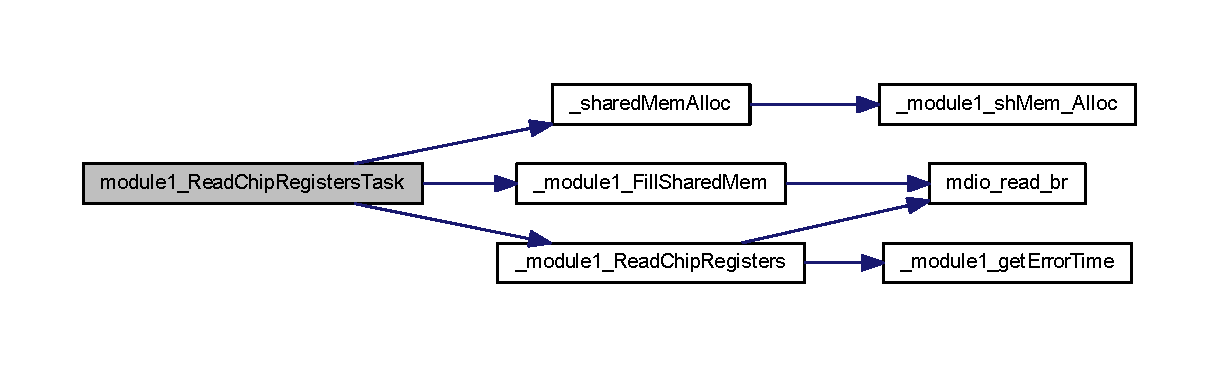
\includegraphics[width=350pt]{module_one_read_eth_phy_8h_ab4a7c038fb29787895e96b7521eede34_cgraph}
\end{center}
\end{figure}


\subsection{Variable Documentation}
\mbox{\Hypertarget{module_one_read_eth_phy_8h_ab6154d17a17c7941b815a06de15f8c54}\label{module_one_read_eth_phy_8h_ab6154d17a17c7941b815a06de15f8c54}} 
\index{module\+One\+Read\+Eth\+Phy.\+h@{module\+One\+Read\+Eth\+Phy.\+h}!\+\_\+diag\+\_\+data\+\_\+struct@{\+\_\+diag\+\_\+data\+\_\+struct}}
\index{\+\_\+diag\+\_\+data\+\_\+struct@{\+\_\+diag\+\_\+data\+\_\+struct}!module\+One\+Read\+Eth\+Phy.\+h@{module\+One\+Read\+Eth\+Phy.\+h}}
\subsubsection{\texorpdfstring{\+\_\+diag\+\_\+data\+\_\+struct}{\_diag\_data\_struct}}
{\footnotesize\ttfamily \mbox{\hyperlink{module_one_read_eth_phy_8h_a58c449f6052675fb4288c20122741cb8}{s\+\_\+\+D\+I\+A\+G\+\_\+\+D\+A\+TA}} \+\_\+diag\+\_\+data\+\_\+struct}

\mbox{\Hypertarget{module_one_read_eth_phy_8h_ac83d0a83ca252211302d67059d2b781e}\label{module_one_read_eth_phy_8h_ac83d0a83ca252211302d67059d2b781e}} 
\index{module\+One\+Read\+Eth\+Phy.\+h@{module\+One\+Read\+Eth\+Phy.\+h}!\+\_\+diag\+\_\+shm\+\_\+ptr@{\+\_\+diag\+\_\+shm\+\_\+ptr}}
\index{\+\_\+diag\+\_\+shm\+\_\+ptr@{\+\_\+diag\+\_\+shm\+\_\+ptr}!module\+One\+Read\+Eth\+Phy.\+h@{module\+One\+Read\+Eth\+Phy.\+h}}
\subsubsection{\texorpdfstring{\+\_\+diag\+\_\+shm\+\_\+ptr}{\_diag\_shm\_ptr}}
{\footnotesize\ttfamily \mbox{\hyperlink{module_one_read_eth_phy_8h_a1f542cc6438c66026963a340365d442a}{s\+\_\+\+D\+I\+A\+G\+\_\+\+S\+H\+M\+\_\+\+D\+A\+TA}}$\ast$ \+\_\+diag\+\_\+shm\+\_\+ptr}

\mbox{\Hypertarget{module_one_read_eth_phy_8h_a6ae24b34485eed59336d11223d848886}\label{module_one_read_eth_phy_8h_a6ae24b34485eed59336d11223d848886}} 
\index{module\+One\+Read\+Eth\+Phy.\+h@{module\+One\+Read\+Eth\+Phy.\+h}!diag\+Msg\+Q\+Id@{diag\+Msg\+Q\+Id}}
\index{diag\+Msg\+Q\+Id@{diag\+Msg\+Q\+Id}!module\+One\+Read\+Eth\+Phy.\+h@{module\+One\+Read\+Eth\+Phy.\+h}}
\subsubsection{\texorpdfstring{diag\+Msg\+Q\+Id}{diagMsgQId}}
{\footnotesize\ttfamily M\+S\+G\+\_\+\+Q\+\_\+\+ID diag\+Msg\+Q\+Id}

\mbox{\Hypertarget{module_one_read_eth_phy_8h_a30a534f860e9976401cc923843ef91c7}\label{module_one_read_eth_phy_8h_a30a534f860e9976401cc923843ef91c7}} 
\index{module\+One\+Read\+Eth\+Phy.\+h@{module\+One\+Read\+Eth\+Phy.\+h}!phy\+Gmii\+Address@{phy\+Gmii\+Address}}
\index{phy\+Gmii\+Address@{phy\+Gmii\+Address}!module\+One\+Read\+Eth\+Phy.\+h@{module\+One\+Read\+Eth\+Phy.\+h}}
\subsubsection{\texorpdfstring{phy\+Gmii\+Address}{phyGmiiAddress}}
{\footnotesize\ttfamily volatile uint32\+\_\+t$\ast$ phy\+Gmii\+Address}

\mbox{\Hypertarget{module_one_read_eth_phy_8h_a552978b3e139f218293760bfa8b8dfaa}\label{module_one_read_eth_phy_8h_a552978b3e139f218293760bfa8b8dfaa}} 
\index{module\+One\+Read\+Eth\+Phy.\+h@{module\+One\+Read\+Eth\+Phy.\+h}!phy\+Gmii\+Data@{phy\+Gmii\+Data}}
\index{phy\+Gmii\+Data@{phy\+Gmii\+Data}!module\+One\+Read\+Eth\+Phy.\+h@{module\+One\+Read\+Eth\+Phy.\+h}}
\subsubsection{\texorpdfstring{phy\+Gmii\+Data}{phyGmiiData}}
{\footnotesize\ttfamily volatile uint32\+\_\+t$\ast$ phy\+Gmii\+Data}


\hypertarget{module_one_startup_8c}{}\section{module\+One\+Startup.\+c File Reference}
\label{module_one_startup_8c}\index{module\+One\+Startup.\+c@{module\+One\+Startup.\+c}}


Interface functions for starting module that are used in \mbox{\hyperlink{tttech_broad_r_reach_8c}{tttech\+Broad\+R\+Reach.\+c}} file. Functions for initializing P\+HY, creating message queues, configuring ethernet interface, starting tasks and RT process (module\+Two).  


{\ttfamily \#include $<$vxworks.\+h$>$}\newline
{\ttfamily \#include $<$stdio.\+h$>$}\newline
{\ttfamily \#include $<$msg\+Q\+Lib\+Common.\+h$>$}\newline
{\ttfamily \#include $<$vm\+Lib\+Common.\+h$>$}\newline
{\ttfamily \#include $<$rtp\+Libcommon.\+h$>$}\newline
{\ttfamily \#include $<$task\+Libcommon.\+h$>$}\newline
{\ttfamily \#include $<$pmap\+Lib.\+h$>$}\newline
{\ttfamily \#include $<$net/utils/ifconfig.\+h$>$}\newline
{\ttfamily \#include \char`\"{}module\+One\+Handle\+Routines.\+h\char`\"{}}\newline
{\ttfamily \#include \char`\"{}module\+One\+Startup.\+h\char`\"{}}\newline
{\ttfamily \#include \char`\"{}module\+One\+Read\+Eth\+Phy.\+h\char`\"{}}\newline
Include dependency graph for module\+One\+Startup.\+c\+:
\nopagebreak
\begin{figure}[H]
\begin{center}
\leavevmode
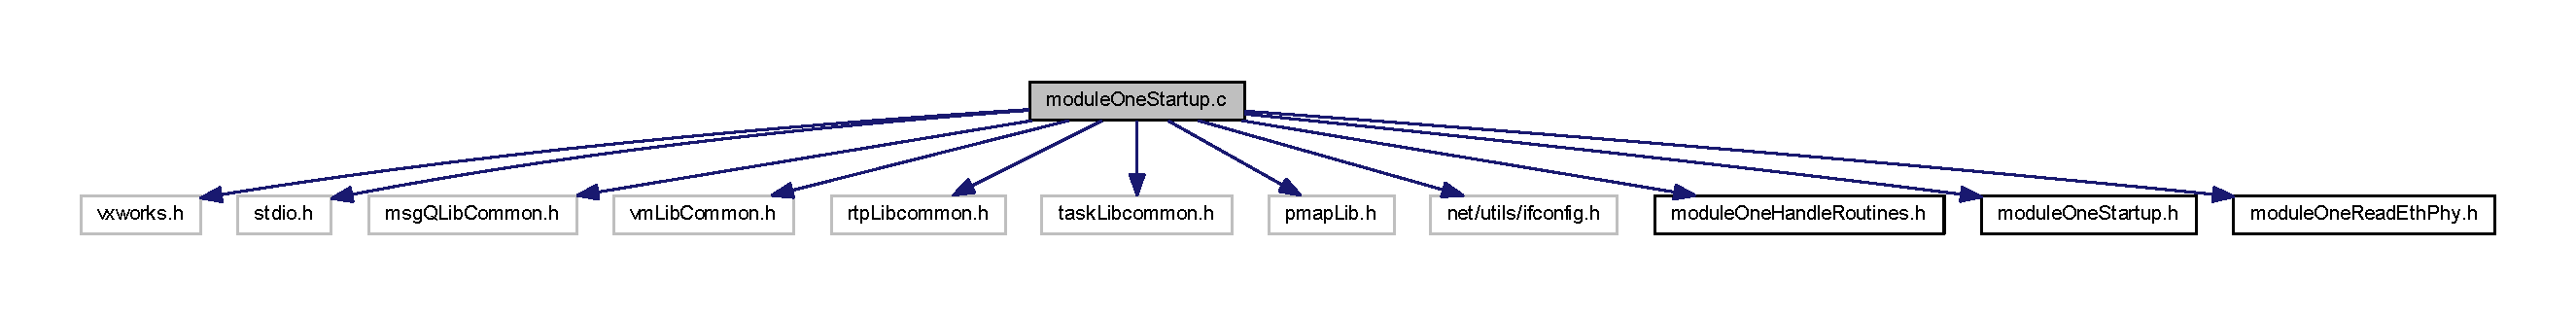
\includegraphics[width=350pt]{module_one_startup_8c__incl}
\end{center}
\end{figure}
\subsection*{Functions}
\begin{DoxyCompactItemize}
\item 
L\+O\+C\+AL S\+T\+A\+T\+US \mbox{\hyperlink{module_one_startup_8c_a099fd2ed34be94194a2365c974416637}{\+\_\+module1\+\_\+\+Create\+Msg\+Queues}} (void)
\item 
void \mbox{\hyperlink{module_one_startup_8c_a79652bed082e520034848c4418a7b5f2}{module1\+\_\+\+Init\+Phy}} (void)
\begin{DoxyCompactList}\small\item\em Init function for eth phy chip interface. \end{DoxyCompactList}\item 
S\+T\+A\+T\+US \mbox{\hyperlink{module_one_startup_8c_ae66f7a060103dcd1441b15d39845cab7}{rtp\+Module}} (void)
\begin{DoxyCompactList}\small\item\em Initial function for starting R\+TP task in user space. \end{DoxyCompactList}\item 
void \mbox{\hyperlink{module_one_startup_8c_a33e10b04aa05e68980ba8cd27d86f51e}{module1\+\_\+\+Start\+Tasks}} (void)
\begin{DoxyCompactList}\small\item\em Functions for starting module 1 tasks for reading E\+TH P\+HY chip registers and retrieving test mode numbers.  S\+T\+A\+V1 13 Assembler instructions that tool can\textquotesingle{}t handle. \end{DoxyCompactList}\item 
void \mbox{\hyperlink{module_one_startup_8c_a91042455237b23c8e02334dc2ad5f779}{module1\+\_\+\+Configure\+Eth\+Interface}} (void)
\begin{DoxyCompactList}\small\item\em Configures hmi0 ethernet interface. \end{DoxyCompactList}\item 
void \mbox{\hyperlink{module_one_startup_8c_a87cefb3488669012643b8b9330086f0d}{module1\+\_\+\+Configure\+V\+L\+AN}} (void)
\begin{DoxyCompactList}\small\item\em Configures V\+L\+AN interface. \end{DoxyCompactList}\end{DoxyCompactItemize}
\subsection*{Variables}
\begin{DoxyCompactItemize}
\item 
M\+S\+G\+\_\+\+Q\+\_\+\+ID \mbox{\hyperlink{module_one_startup_8c_a7399395bce7dd3dd0341d0b7d7e78ec9}{routines\+Msg\+Q\+Id}} = M\+S\+G\+\_\+\+Q\+\_\+\+I\+D\+\_\+\+N\+U\+LL
\item 
M\+S\+G\+\_\+\+Q\+\_\+\+ID \mbox{\hyperlink{module_one_startup_8c_a6ae24b34485eed59336d11223d848886}{diag\+Msg\+Q\+Id}} = M\+S\+G\+\_\+\+Q\+\_\+\+I\+D\+\_\+\+N\+U\+LL
\item 
volatile uint32\+\_\+t $\ast$ \mbox{\hyperlink{module_one_startup_8c_a30a534f860e9976401cc923843ef91c7}{phy\+Gmii\+Address}}
\item 
volatile uint32\+\_\+t $\ast$ \mbox{\hyperlink{module_one_startup_8c_a552978b3e139f218293760bfa8b8dfaa}{phy\+Gmii\+Data}}
\end{DoxyCompactItemize}


\subsection{Detailed Description}
Interface functions for starting module that are used in \mbox{\hyperlink{tttech_broad_r_reach_8c}{tttech\+Broad\+R\+Reach.\+c}} file. Functions for initializing P\+HY, creating message queues, configuring ethernet interface, starting tasks and RT process (module\+Two). 

\mbox{\hyperlink{module_one_startup_8c}{module\+One\+Startup.\+c}}

\begin{DoxyVersion}{Version}
\mbox{[}19-\/\+Apr-\/2018\mbox{]} \mbox{[}Stefan Masalusic\mbox{]} Initial creation
\end{DoxyVersion}
\mbox{[}19-\/\+Apr-\/2018\mbox{]} Added Init\+Phy and Create\+Msg\+Queues functions \mbox{[}23-\/\+Apr-\/2018\mbox{]} Added Start\+Tasks function \mbox{[}25-\/\+Apr-\/2018\mbox{]} Added Configure\+Eth\+Interface and Configure\+V\+L\+A\+N\+Interface functions \mbox{[}18-\/\+May-\/2018\mbox{]} Added rtp\+Module function \mbox{[}24-\/\+May-\/2018\mbox{]} Added function descriptions 



\subsection{Function Documentation}
\mbox{\Hypertarget{module_one_startup_8c_a099fd2ed34be94194a2365c974416637}\label{module_one_startup_8c_a099fd2ed34be94194a2365c974416637}} 
\index{module\+One\+Startup.\+c@{module\+One\+Startup.\+c}!\+\_\+module1\+\_\+\+Create\+Msg\+Queues@{\+\_\+module1\+\_\+\+Create\+Msg\+Queues}}
\index{\+\_\+module1\+\_\+\+Create\+Msg\+Queues@{\+\_\+module1\+\_\+\+Create\+Msg\+Queues}!module\+One\+Startup.\+c@{module\+One\+Startup.\+c}}
\subsubsection{\texorpdfstring{\+\_\+module1\+\_\+\+Create\+Msg\+Queues()}{\_module1\_CreateMsgQueues()}}
{\footnotesize\ttfamily L\+O\+C\+AL S\+T\+A\+T\+US \+\_\+module1\+\_\+\+Create\+Msg\+Queues (\begin{DoxyParamCaption}\item[{void}]{ }\end{DoxyParamCaption})}

\mbox{\Hypertarget{module_one_startup_8c_a91042455237b23c8e02334dc2ad5f779}\label{module_one_startup_8c_a91042455237b23c8e02334dc2ad5f779}} 
\index{module\+One\+Startup.\+c@{module\+One\+Startup.\+c}!module1\+\_\+\+Configure\+Eth\+Interface@{module1\+\_\+\+Configure\+Eth\+Interface}}
\index{module1\+\_\+\+Configure\+Eth\+Interface@{module1\+\_\+\+Configure\+Eth\+Interface}!module\+One\+Startup.\+c@{module\+One\+Startup.\+c}}
\subsubsection{\texorpdfstring{module1\+\_\+\+Configure\+Eth\+Interface()}{module1\_ConfigureEthInterface()}}
{\footnotesize\ttfamily void module1\+\_\+\+Configure\+Eth\+Interface (\begin{DoxyParamCaption}\item[{void}]{ }\end{DoxyParamCaption})}



Configures hmi0 ethernet interface. 

\mbox{\Hypertarget{module_one_startup_8c_a87cefb3488669012643b8b9330086f0d}\label{module_one_startup_8c_a87cefb3488669012643b8b9330086f0d}} 
\index{module\+One\+Startup.\+c@{module\+One\+Startup.\+c}!module1\+\_\+\+Configure\+V\+L\+AN@{module1\+\_\+\+Configure\+V\+L\+AN}}
\index{module1\+\_\+\+Configure\+V\+L\+AN@{module1\+\_\+\+Configure\+V\+L\+AN}!module\+One\+Startup.\+c@{module\+One\+Startup.\+c}}
\subsubsection{\texorpdfstring{module1\+\_\+\+Configure\+V\+L\+A\+N()}{module1\_ConfigureVLAN()}}
{\footnotesize\ttfamily void module1\+\_\+\+Configure\+V\+L\+AN (\begin{DoxyParamCaption}\item[{void}]{ }\end{DoxyParamCaption})}



Configures V\+L\+AN interface. 

\mbox{\Hypertarget{module_one_startup_8c_a79652bed082e520034848c4418a7b5f2}\label{module_one_startup_8c_a79652bed082e520034848c4418a7b5f2}} 
\index{module\+One\+Startup.\+c@{module\+One\+Startup.\+c}!module1\+\_\+\+Init\+Phy@{module1\+\_\+\+Init\+Phy}}
\index{module1\+\_\+\+Init\+Phy@{module1\+\_\+\+Init\+Phy}!module\+One\+Startup.\+c@{module\+One\+Startup.\+c}}
\subsubsection{\texorpdfstring{module1\+\_\+\+Init\+Phy()}{module1\_InitPhy()}}
{\footnotesize\ttfamily void module1\+\_\+\+Init\+Phy (\begin{DoxyParamCaption}\item[{void}]{ }\end{DoxyParamCaption})}



Init function for eth phy chip interface. 

Here is the call graph for this function\+:
\nopagebreak
\begin{figure}[H]
\begin{center}
\leavevmode
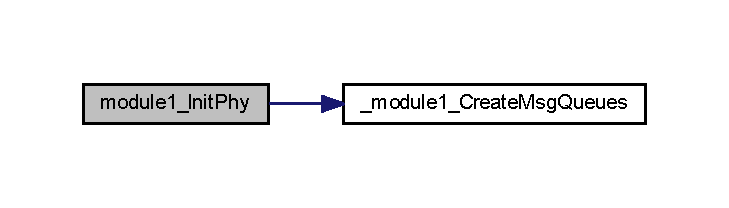
\includegraphics[width=350pt]{module_one_startup_8c_a79652bed082e520034848c4418a7b5f2_cgraph}
\end{center}
\end{figure}
\mbox{\Hypertarget{module_one_startup_8c_a33e10b04aa05e68980ba8cd27d86f51e}\label{module_one_startup_8c_a33e10b04aa05e68980ba8cd27d86f51e}} 
\index{module\+One\+Startup.\+c@{module\+One\+Startup.\+c}!module1\+\_\+\+Start\+Tasks@{module1\+\_\+\+Start\+Tasks}}
\index{module1\+\_\+\+Start\+Tasks@{module1\+\_\+\+Start\+Tasks}!module\+One\+Startup.\+c@{module\+One\+Startup.\+c}}
\subsubsection{\texorpdfstring{module1\+\_\+\+Start\+Tasks()}{module1\_StartTasks()}}
{\footnotesize\ttfamily void module1\+\_\+\+Start\+Tasks (\begin{DoxyParamCaption}\item[{void}]{ }\end{DoxyParamCaption})}



Functions for starting module 1 tasks for reading E\+TH P\+HY chip registers and retrieving test mode numbers.  S\+T\+A\+V1 13 Assembler instructions that tool can\textquotesingle{}t handle. 

Here is the call graph for this function\+:
\nopagebreak
\begin{figure}[H]
\begin{center}
\leavevmode
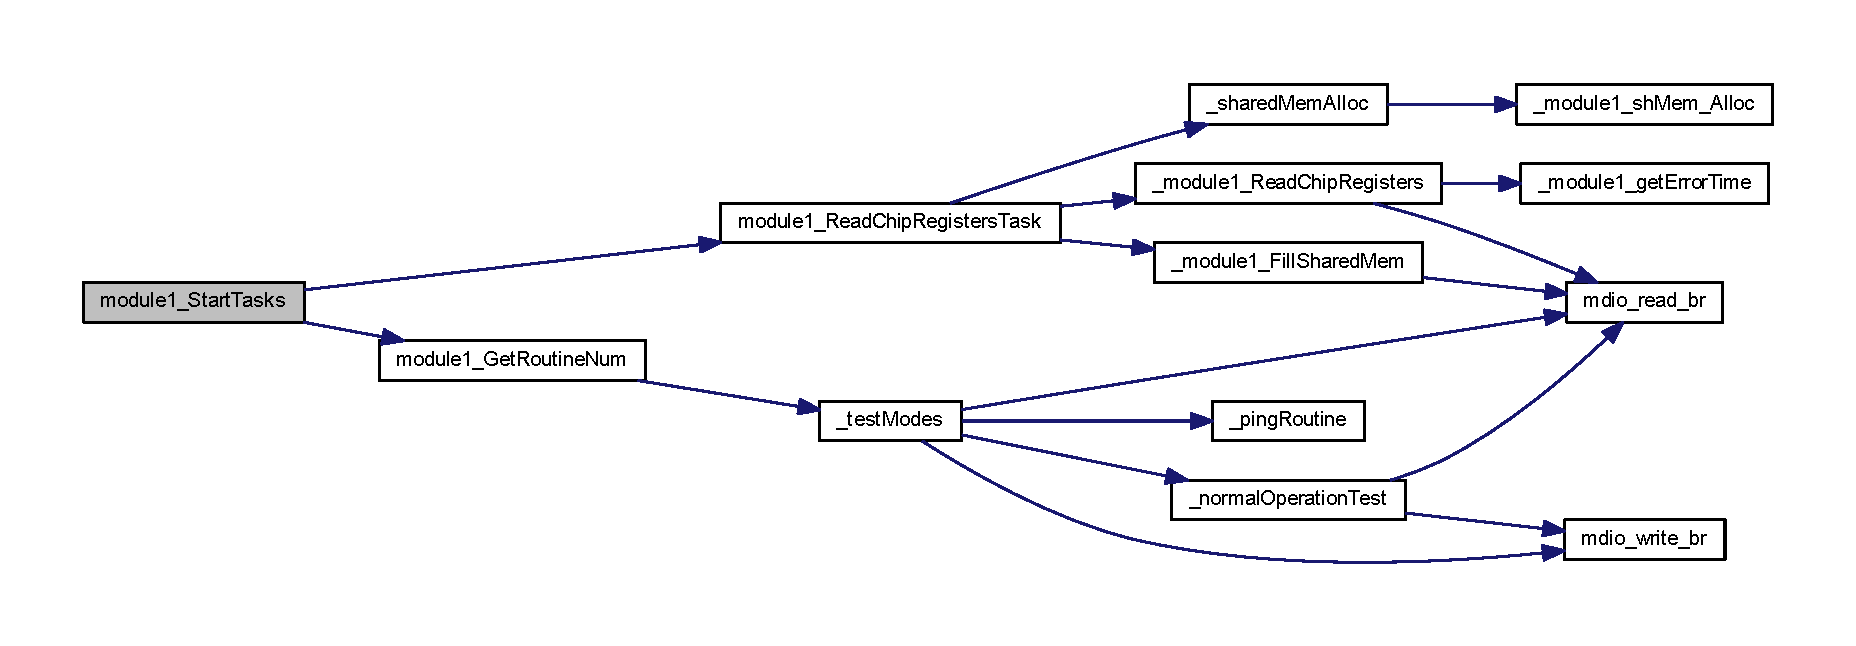
\includegraphics[width=350pt]{module_one_startup_8c_a33e10b04aa05e68980ba8cd27d86f51e_cgraph}
\end{center}
\end{figure}
\mbox{\Hypertarget{module_one_startup_8c_ae66f7a060103dcd1441b15d39845cab7}\label{module_one_startup_8c_ae66f7a060103dcd1441b15d39845cab7}} 
\index{module\+One\+Startup.\+c@{module\+One\+Startup.\+c}!rtp\+Module@{rtp\+Module}}
\index{rtp\+Module@{rtp\+Module}!module\+One\+Startup.\+c@{module\+One\+Startup.\+c}}
\subsubsection{\texorpdfstring{rtp\+Module()}{rtpModule()}}
{\footnotesize\ttfamily S\+T\+A\+T\+US rtp\+Module (\begin{DoxyParamCaption}\item[{void}]{ }\end{DoxyParamCaption})}



Initial function for starting R\+TP task in user space. 

\begin{DoxyReturn}{Returns}
OK if successful, E\+R\+R\+OR otherwise  E\+R\+R\+OR if rtp\+Spawn() function fails 
\end{DoxyReturn}


\subsection{Variable Documentation}
\mbox{\Hypertarget{module_one_startup_8c_a6ae24b34485eed59336d11223d848886}\label{module_one_startup_8c_a6ae24b34485eed59336d11223d848886}} 
\index{module\+One\+Startup.\+c@{module\+One\+Startup.\+c}!diag\+Msg\+Q\+Id@{diag\+Msg\+Q\+Id}}
\index{diag\+Msg\+Q\+Id@{diag\+Msg\+Q\+Id}!module\+One\+Startup.\+c@{module\+One\+Startup.\+c}}
\subsubsection{\texorpdfstring{diag\+Msg\+Q\+Id}{diagMsgQId}}
{\footnotesize\ttfamily M\+S\+G\+\_\+\+Q\+\_\+\+ID diag\+Msg\+Q\+Id = M\+S\+G\+\_\+\+Q\+\_\+\+I\+D\+\_\+\+N\+U\+LL}

\mbox{\Hypertarget{module_one_startup_8c_a30a534f860e9976401cc923843ef91c7}\label{module_one_startup_8c_a30a534f860e9976401cc923843ef91c7}} 
\index{module\+One\+Startup.\+c@{module\+One\+Startup.\+c}!phy\+Gmii\+Address@{phy\+Gmii\+Address}}
\index{phy\+Gmii\+Address@{phy\+Gmii\+Address}!module\+One\+Startup.\+c@{module\+One\+Startup.\+c}}
\subsubsection{\texorpdfstring{phy\+Gmii\+Address}{phyGmiiAddress}}
{\footnotesize\ttfamily volatile uint32\+\_\+t$\ast$ phy\+Gmii\+Address}

\mbox{\Hypertarget{module_one_startup_8c_a552978b3e139f218293760bfa8b8dfaa}\label{module_one_startup_8c_a552978b3e139f218293760bfa8b8dfaa}} 
\index{module\+One\+Startup.\+c@{module\+One\+Startup.\+c}!phy\+Gmii\+Data@{phy\+Gmii\+Data}}
\index{phy\+Gmii\+Data@{phy\+Gmii\+Data}!module\+One\+Startup.\+c@{module\+One\+Startup.\+c}}
\subsubsection{\texorpdfstring{phy\+Gmii\+Data}{phyGmiiData}}
{\footnotesize\ttfamily volatile uint32\+\_\+t$\ast$ phy\+Gmii\+Data}

\mbox{\Hypertarget{module_one_startup_8c_a7399395bce7dd3dd0341d0b7d7e78ec9}\label{module_one_startup_8c_a7399395bce7dd3dd0341d0b7d7e78ec9}} 
\index{module\+One\+Startup.\+c@{module\+One\+Startup.\+c}!routines\+Msg\+Q\+Id@{routines\+Msg\+Q\+Id}}
\index{routines\+Msg\+Q\+Id@{routines\+Msg\+Q\+Id}!module\+One\+Startup.\+c@{module\+One\+Startup.\+c}}
\subsubsection{\texorpdfstring{routines\+Msg\+Q\+Id}{routinesMsgQId}}
{\footnotesize\ttfamily M\+S\+G\+\_\+\+Q\+\_\+\+ID routines\+Msg\+Q\+Id = M\+S\+G\+\_\+\+Q\+\_\+\+I\+D\+\_\+\+N\+U\+LL}


\hypertarget{module_one_startup_8h}{}\section{module\+One\+Startup.\+h File Reference}
\label{module_one_startup_8h}\index{module\+One\+Startup.\+h@{module\+One\+Startup.\+h}}
This graph shows which files directly or indirectly include this file\+:
\nopagebreak
\begin{figure}[H]
\begin{center}
\leavevmode
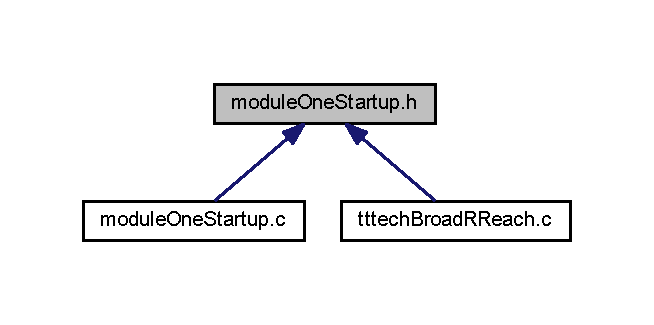
\includegraphics[width=314pt]{module_one_startup_8h__dep__incl}
\end{center}
\end{figure}
\subsection*{Macros}
\begin{DoxyCompactItemize}
\item 
\#define \mbox{\hyperlink{module_one_startup_8h_ab3d937239da9b96a62a28e2b63931609}{B\+Y\+T\+E\+S\+\_\+\+N\+UM}}~(0x\+F\+F)
\item 
\#define \mbox{\hyperlink{module_one_startup_8h_ab479861fbeb542421a059450bf96190b}{C\+Y\+C\+L\+O\+N\+E\+\_\+\+A\+D\+D\+R\+E\+S\+S\+\_\+\+R\+E\+G\+I\+S\+T\+E\+R\+\_\+\+O\+F\+F\+S\+ET}}~(0x10\+U)
\item 
\#define \mbox{\hyperlink{module_one_startup_8h_a2ee53712d2a6b91d23d9c32bb5e0a141}{C\+Y\+C\+L\+O\+N\+E\+\_\+\+D\+A\+T\+A\+\_\+\+R\+E\+G\+I\+S\+T\+E\+R\+\_\+\+O\+F\+F\+S\+ET}}~(0x14\+U)
\item 
\#define \mbox{\hyperlink{module_one_startup_8h_ae8e9cbf781a806bd4dd34345e77c52fe}{R\+T\+P\+R\+O\+C\+E\+S\+S\+\_\+\+T\+A\+S\+K\+\_\+\+P\+R\+I\+O\+R\+I\+TY}}~(207)
\item 
\#define \mbox{\hyperlink{module_one_startup_8h_a3ab7b5b11b21b53cfced874a4ca7ac32}{R\+T\+P\+R\+O\+C\+E\+S\+S\+\_\+\+S\+T\+A\+C\+K\+\_\+\+S\+I\+ZE}}~(0x19000)
\item 
\#define \mbox{\hyperlink{module_one_startup_8h_ac7370c3ab42bdeb517ee4349e7087828}{R\+T\+P\+R\+O\+C\+E\+S\+S\+\_\+\+G\+L\+O\+B\+A\+L\+\_\+\+S\+Y\+M\+B\+O\+LS}}~(0x01)
\item 
\#define \mbox{\hyperlink{module_one_startup_8h_a8d62b95e7a0fed63c7e2db18ee0695ce}{D\+I\+A\+G\+\_\+\+T\+A\+S\+K\+\_\+\+P\+R\+I\+O\+R\+I\+TY}}~(202)
\item 
\#define \mbox{\hyperlink{module_one_startup_8h_a334fb2873a136829fc34ac52223b1655}{D\+I\+A\+G\+\_\+\+S\+T\+A\+C\+K\+\_\+\+S\+I\+ZE}}~(2000)
\item 
\#define \mbox{\hyperlink{module_one_startup_8h_ab365e2f37dd1db89ce8dc3c1e49fd7d4}{R\+O\+U\+T\+I\+N\+E\+S\+\_\+\+T\+A\+S\+K\+\_\+\+P\+R\+I\+O\+R\+I\+TY}}~(204)
\item 
\#define \mbox{\hyperlink{module_one_startup_8h_aa554f4dc2858ac360710aebbc87f6072}{R\+O\+U\+T\+I\+N\+E\+S\+\_\+\+S\+T\+A\+C\+K\+\_\+\+S\+I\+ZE}}~(100)
\end{DoxyCompactItemize}
\subsection*{Functions}
\begin{DoxyCompactItemize}
\item 
void \mbox{\hyperlink{module_one_startup_8h_a79652bed082e520034848c4418a7b5f2}{module1\+\_\+\+Init\+Phy}} (void)
\begin{DoxyCompactList}\small\item\em Init function for eth phy chip interface. \end{DoxyCompactList}\item 
S\+T\+A\+T\+US \mbox{\hyperlink{module_one_startup_8h_ae66f7a060103dcd1441b15d39845cab7}{rtp\+Module}} (void)
\begin{DoxyCompactList}\small\item\em Initial function for starting R\+TP task in user space. \end{DoxyCompactList}\item 
void \mbox{\hyperlink{module_one_startup_8h_a33e10b04aa05e68980ba8cd27d86f51e}{module1\+\_\+\+Start\+Tasks}} (void)
\begin{DoxyCompactList}\small\item\em Functions for starting module 1 tasks for reading E\+TH P\+HY chip registers and retrieving test mode numbers.  S\+T\+A\+V1 13 Assembler instructions that tool can\textquotesingle{}t handle. \end{DoxyCompactList}\item 
void \mbox{\hyperlink{module_one_startup_8h_a91042455237b23c8e02334dc2ad5f779}{module1\+\_\+\+Configure\+Eth\+Interface}} (void)
\begin{DoxyCompactList}\small\item\em Configures hmi0 ethernet interface. \end{DoxyCompactList}\item 
void \mbox{\hyperlink{module_one_startup_8h_a87cefb3488669012643b8b9330086f0d}{module1\+\_\+\+Configure\+V\+L\+AN}} (void)
\begin{DoxyCompactList}\small\item\em Configures V\+L\+AN interface. \end{DoxyCompactList}\end{DoxyCompactItemize}


\subsection{Macro Definition Documentation}
\mbox{\Hypertarget{module_one_startup_8h_ab3d937239da9b96a62a28e2b63931609}\label{module_one_startup_8h_ab3d937239da9b96a62a28e2b63931609}} 
\index{module\+One\+Startup.\+h@{module\+One\+Startup.\+h}!B\+Y\+T\+E\+S\+\_\+\+N\+UM@{B\+Y\+T\+E\+S\+\_\+\+N\+UM}}
\index{B\+Y\+T\+E\+S\+\_\+\+N\+UM@{B\+Y\+T\+E\+S\+\_\+\+N\+UM}!module\+One\+Startup.\+h@{module\+One\+Startup.\+h}}
\subsubsection{\texorpdfstring{B\+Y\+T\+E\+S\+\_\+\+N\+UM}{BYTES\_NUM}}
{\footnotesize\ttfamily \#define B\+Y\+T\+E\+S\+\_\+\+N\+UM~(0x\+F\+F)}

\mbox{\Hypertarget{module_one_startup_8h_ab479861fbeb542421a059450bf96190b}\label{module_one_startup_8h_ab479861fbeb542421a059450bf96190b}} 
\index{module\+One\+Startup.\+h@{module\+One\+Startup.\+h}!C\+Y\+C\+L\+O\+N\+E\+\_\+\+A\+D\+D\+R\+E\+S\+S\+\_\+\+R\+E\+G\+I\+S\+T\+E\+R\+\_\+\+O\+F\+F\+S\+ET@{C\+Y\+C\+L\+O\+N\+E\+\_\+\+A\+D\+D\+R\+E\+S\+S\+\_\+\+R\+E\+G\+I\+S\+T\+E\+R\+\_\+\+O\+F\+F\+S\+ET}}
\index{C\+Y\+C\+L\+O\+N\+E\+\_\+\+A\+D\+D\+R\+E\+S\+S\+\_\+\+R\+E\+G\+I\+S\+T\+E\+R\+\_\+\+O\+F\+F\+S\+ET@{C\+Y\+C\+L\+O\+N\+E\+\_\+\+A\+D\+D\+R\+E\+S\+S\+\_\+\+R\+E\+G\+I\+S\+T\+E\+R\+\_\+\+O\+F\+F\+S\+ET}!module\+One\+Startup.\+h@{module\+One\+Startup.\+h}}
\subsubsection{\texorpdfstring{C\+Y\+C\+L\+O\+N\+E\+\_\+\+A\+D\+D\+R\+E\+S\+S\+\_\+\+R\+E\+G\+I\+S\+T\+E\+R\+\_\+\+O\+F\+F\+S\+ET}{CYCLONE\_ADDRESS\_REGISTER\_OFFSET}}
{\footnotesize\ttfamily \#define C\+Y\+C\+L\+O\+N\+E\+\_\+\+A\+D\+D\+R\+E\+S\+S\+\_\+\+R\+E\+G\+I\+S\+T\+E\+R\+\_\+\+O\+F\+F\+S\+ET~(0x10\+U)}

\mbox{\Hypertarget{module_one_startup_8h_a2ee53712d2a6b91d23d9c32bb5e0a141}\label{module_one_startup_8h_a2ee53712d2a6b91d23d9c32bb5e0a141}} 
\index{module\+One\+Startup.\+h@{module\+One\+Startup.\+h}!C\+Y\+C\+L\+O\+N\+E\+\_\+\+D\+A\+T\+A\+\_\+\+R\+E\+G\+I\+S\+T\+E\+R\+\_\+\+O\+F\+F\+S\+ET@{C\+Y\+C\+L\+O\+N\+E\+\_\+\+D\+A\+T\+A\+\_\+\+R\+E\+G\+I\+S\+T\+E\+R\+\_\+\+O\+F\+F\+S\+ET}}
\index{C\+Y\+C\+L\+O\+N\+E\+\_\+\+D\+A\+T\+A\+\_\+\+R\+E\+G\+I\+S\+T\+E\+R\+\_\+\+O\+F\+F\+S\+ET@{C\+Y\+C\+L\+O\+N\+E\+\_\+\+D\+A\+T\+A\+\_\+\+R\+E\+G\+I\+S\+T\+E\+R\+\_\+\+O\+F\+F\+S\+ET}!module\+One\+Startup.\+h@{module\+One\+Startup.\+h}}
\subsubsection{\texorpdfstring{C\+Y\+C\+L\+O\+N\+E\+\_\+\+D\+A\+T\+A\+\_\+\+R\+E\+G\+I\+S\+T\+E\+R\+\_\+\+O\+F\+F\+S\+ET}{CYCLONE\_DATA\_REGISTER\_OFFSET}}
{\footnotesize\ttfamily \#define C\+Y\+C\+L\+O\+N\+E\+\_\+\+D\+A\+T\+A\+\_\+\+R\+E\+G\+I\+S\+T\+E\+R\+\_\+\+O\+F\+F\+S\+ET~(0x14\+U)}

\mbox{\Hypertarget{module_one_startup_8h_a334fb2873a136829fc34ac52223b1655}\label{module_one_startup_8h_a334fb2873a136829fc34ac52223b1655}} 
\index{module\+One\+Startup.\+h@{module\+One\+Startup.\+h}!D\+I\+A\+G\+\_\+\+S\+T\+A\+C\+K\+\_\+\+S\+I\+ZE@{D\+I\+A\+G\+\_\+\+S\+T\+A\+C\+K\+\_\+\+S\+I\+ZE}}
\index{D\+I\+A\+G\+\_\+\+S\+T\+A\+C\+K\+\_\+\+S\+I\+ZE@{D\+I\+A\+G\+\_\+\+S\+T\+A\+C\+K\+\_\+\+S\+I\+ZE}!module\+One\+Startup.\+h@{module\+One\+Startup.\+h}}
\subsubsection{\texorpdfstring{D\+I\+A\+G\+\_\+\+S\+T\+A\+C\+K\+\_\+\+S\+I\+ZE}{DIAG\_STACK\_SIZE}}
{\footnotesize\ttfamily \#define D\+I\+A\+G\+\_\+\+S\+T\+A\+C\+K\+\_\+\+S\+I\+ZE~(2000)}

\mbox{\Hypertarget{module_one_startup_8h_a8d62b95e7a0fed63c7e2db18ee0695ce}\label{module_one_startup_8h_a8d62b95e7a0fed63c7e2db18ee0695ce}} 
\index{module\+One\+Startup.\+h@{module\+One\+Startup.\+h}!D\+I\+A\+G\+\_\+\+T\+A\+S\+K\+\_\+\+P\+R\+I\+O\+R\+I\+TY@{D\+I\+A\+G\+\_\+\+T\+A\+S\+K\+\_\+\+P\+R\+I\+O\+R\+I\+TY}}
\index{D\+I\+A\+G\+\_\+\+T\+A\+S\+K\+\_\+\+P\+R\+I\+O\+R\+I\+TY@{D\+I\+A\+G\+\_\+\+T\+A\+S\+K\+\_\+\+P\+R\+I\+O\+R\+I\+TY}!module\+One\+Startup.\+h@{module\+One\+Startup.\+h}}
\subsubsection{\texorpdfstring{D\+I\+A\+G\+\_\+\+T\+A\+S\+K\+\_\+\+P\+R\+I\+O\+R\+I\+TY}{DIAG\_TASK\_PRIORITY}}
{\footnotesize\ttfamily \#define D\+I\+A\+G\+\_\+\+T\+A\+S\+K\+\_\+\+P\+R\+I\+O\+R\+I\+TY~(202)}

\mbox{\Hypertarget{module_one_startup_8h_aa554f4dc2858ac360710aebbc87f6072}\label{module_one_startup_8h_aa554f4dc2858ac360710aebbc87f6072}} 
\index{module\+One\+Startup.\+h@{module\+One\+Startup.\+h}!R\+O\+U\+T\+I\+N\+E\+S\+\_\+\+S\+T\+A\+C\+K\+\_\+\+S\+I\+ZE@{R\+O\+U\+T\+I\+N\+E\+S\+\_\+\+S\+T\+A\+C\+K\+\_\+\+S\+I\+ZE}}
\index{R\+O\+U\+T\+I\+N\+E\+S\+\_\+\+S\+T\+A\+C\+K\+\_\+\+S\+I\+ZE@{R\+O\+U\+T\+I\+N\+E\+S\+\_\+\+S\+T\+A\+C\+K\+\_\+\+S\+I\+ZE}!module\+One\+Startup.\+h@{module\+One\+Startup.\+h}}
\subsubsection{\texorpdfstring{R\+O\+U\+T\+I\+N\+E\+S\+\_\+\+S\+T\+A\+C\+K\+\_\+\+S\+I\+ZE}{ROUTINES\_STACK\_SIZE}}
{\footnotesize\ttfamily \#define R\+O\+U\+T\+I\+N\+E\+S\+\_\+\+S\+T\+A\+C\+K\+\_\+\+S\+I\+ZE~(100)}

\mbox{\Hypertarget{module_one_startup_8h_ab365e2f37dd1db89ce8dc3c1e49fd7d4}\label{module_one_startup_8h_ab365e2f37dd1db89ce8dc3c1e49fd7d4}} 
\index{module\+One\+Startup.\+h@{module\+One\+Startup.\+h}!R\+O\+U\+T\+I\+N\+E\+S\+\_\+\+T\+A\+S\+K\+\_\+\+P\+R\+I\+O\+R\+I\+TY@{R\+O\+U\+T\+I\+N\+E\+S\+\_\+\+T\+A\+S\+K\+\_\+\+P\+R\+I\+O\+R\+I\+TY}}
\index{R\+O\+U\+T\+I\+N\+E\+S\+\_\+\+T\+A\+S\+K\+\_\+\+P\+R\+I\+O\+R\+I\+TY@{R\+O\+U\+T\+I\+N\+E\+S\+\_\+\+T\+A\+S\+K\+\_\+\+P\+R\+I\+O\+R\+I\+TY}!module\+One\+Startup.\+h@{module\+One\+Startup.\+h}}
\subsubsection{\texorpdfstring{R\+O\+U\+T\+I\+N\+E\+S\+\_\+\+T\+A\+S\+K\+\_\+\+P\+R\+I\+O\+R\+I\+TY}{ROUTINES\_TASK\_PRIORITY}}
{\footnotesize\ttfamily \#define R\+O\+U\+T\+I\+N\+E\+S\+\_\+\+T\+A\+S\+K\+\_\+\+P\+R\+I\+O\+R\+I\+TY~(204)}

\mbox{\Hypertarget{module_one_startup_8h_ac7370c3ab42bdeb517ee4349e7087828}\label{module_one_startup_8h_ac7370c3ab42bdeb517ee4349e7087828}} 
\index{module\+One\+Startup.\+h@{module\+One\+Startup.\+h}!R\+T\+P\+R\+O\+C\+E\+S\+S\+\_\+\+G\+L\+O\+B\+A\+L\+\_\+\+S\+Y\+M\+B\+O\+LS@{R\+T\+P\+R\+O\+C\+E\+S\+S\+\_\+\+G\+L\+O\+B\+A\+L\+\_\+\+S\+Y\+M\+B\+O\+LS}}
\index{R\+T\+P\+R\+O\+C\+E\+S\+S\+\_\+\+G\+L\+O\+B\+A\+L\+\_\+\+S\+Y\+M\+B\+O\+LS@{R\+T\+P\+R\+O\+C\+E\+S\+S\+\_\+\+G\+L\+O\+B\+A\+L\+\_\+\+S\+Y\+M\+B\+O\+LS}!module\+One\+Startup.\+h@{module\+One\+Startup.\+h}}
\subsubsection{\texorpdfstring{R\+T\+P\+R\+O\+C\+E\+S\+S\+\_\+\+G\+L\+O\+B\+A\+L\+\_\+\+S\+Y\+M\+B\+O\+LS}{RTPROCESS\_GLOBAL\_SYMBOLS}}
{\footnotesize\ttfamily \#define R\+T\+P\+R\+O\+C\+E\+S\+S\+\_\+\+G\+L\+O\+B\+A\+L\+\_\+\+S\+Y\+M\+B\+O\+LS~(0x01)}

\mbox{\Hypertarget{module_one_startup_8h_a3ab7b5b11b21b53cfced874a4ca7ac32}\label{module_one_startup_8h_a3ab7b5b11b21b53cfced874a4ca7ac32}} 
\index{module\+One\+Startup.\+h@{module\+One\+Startup.\+h}!R\+T\+P\+R\+O\+C\+E\+S\+S\+\_\+\+S\+T\+A\+C\+K\+\_\+\+S\+I\+ZE@{R\+T\+P\+R\+O\+C\+E\+S\+S\+\_\+\+S\+T\+A\+C\+K\+\_\+\+S\+I\+ZE}}
\index{R\+T\+P\+R\+O\+C\+E\+S\+S\+\_\+\+S\+T\+A\+C\+K\+\_\+\+S\+I\+ZE@{R\+T\+P\+R\+O\+C\+E\+S\+S\+\_\+\+S\+T\+A\+C\+K\+\_\+\+S\+I\+ZE}!module\+One\+Startup.\+h@{module\+One\+Startup.\+h}}
\subsubsection{\texorpdfstring{R\+T\+P\+R\+O\+C\+E\+S\+S\+\_\+\+S\+T\+A\+C\+K\+\_\+\+S\+I\+ZE}{RTPROCESS\_STACK\_SIZE}}
{\footnotesize\ttfamily \#define R\+T\+P\+R\+O\+C\+E\+S\+S\+\_\+\+S\+T\+A\+C\+K\+\_\+\+S\+I\+ZE~(0x19000)}

\mbox{\Hypertarget{module_one_startup_8h_ae8e9cbf781a806bd4dd34345e77c52fe}\label{module_one_startup_8h_ae8e9cbf781a806bd4dd34345e77c52fe}} 
\index{module\+One\+Startup.\+h@{module\+One\+Startup.\+h}!R\+T\+P\+R\+O\+C\+E\+S\+S\+\_\+\+T\+A\+S\+K\+\_\+\+P\+R\+I\+O\+R\+I\+TY@{R\+T\+P\+R\+O\+C\+E\+S\+S\+\_\+\+T\+A\+S\+K\+\_\+\+P\+R\+I\+O\+R\+I\+TY}}
\index{R\+T\+P\+R\+O\+C\+E\+S\+S\+\_\+\+T\+A\+S\+K\+\_\+\+P\+R\+I\+O\+R\+I\+TY@{R\+T\+P\+R\+O\+C\+E\+S\+S\+\_\+\+T\+A\+S\+K\+\_\+\+P\+R\+I\+O\+R\+I\+TY}!module\+One\+Startup.\+h@{module\+One\+Startup.\+h}}
\subsubsection{\texorpdfstring{R\+T\+P\+R\+O\+C\+E\+S\+S\+\_\+\+T\+A\+S\+K\+\_\+\+P\+R\+I\+O\+R\+I\+TY}{RTPROCESS\_TASK\_PRIORITY}}
{\footnotesize\ttfamily \#define R\+T\+P\+R\+O\+C\+E\+S\+S\+\_\+\+T\+A\+S\+K\+\_\+\+P\+R\+I\+O\+R\+I\+TY~(207)}



\subsection{Function Documentation}
\mbox{\Hypertarget{module_one_startup_8h_a91042455237b23c8e02334dc2ad5f779}\label{module_one_startup_8h_a91042455237b23c8e02334dc2ad5f779}} 
\index{module\+One\+Startup.\+h@{module\+One\+Startup.\+h}!module1\+\_\+\+Configure\+Eth\+Interface@{module1\+\_\+\+Configure\+Eth\+Interface}}
\index{module1\+\_\+\+Configure\+Eth\+Interface@{module1\+\_\+\+Configure\+Eth\+Interface}!module\+One\+Startup.\+h@{module\+One\+Startup.\+h}}
\subsubsection{\texorpdfstring{module1\+\_\+\+Configure\+Eth\+Interface()}{module1\_ConfigureEthInterface()}}
{\footnotesize\ttfamily void module1\+\_\+\+Configure\+Eth\+Interface (\begin{DoxyParamCaption}\item[{void}]{ }\end{DoxyParamCaption})}



Configures hmi0 ethernet interface. 

\mbox{\Hypertarget{module_one_startup_8h_a87cefb3488669012643b8b9330086f0d}\label{module_one_startup_8h_a87cefb3488669012643b8b9330086f0d}} 
\index{module\+One\+Startup.\+h@{module\+One\+Startup.\+h}!module1\+\_\+\+Configure\+V\+L\+AN@{module1\+\_\+\+Configure\+V\+L\+AN}}
\index{module1\+\_\+\+Configure\+V\+L\+AN@{module1\+\_\+\+Configure\+V\+L\+AN}!module\+One\+Startup.\+h@{module\+One\+Startup.\+h}}
\subsubsection{\texorpdfstring{module1\+\_\+\+Configure\+V\+L\+A\+N()}{module1\_ConfigureVLAN()}}
{\footnotesize\ttfamily void module1\+\_\+\+Configure\+V\+L\+AN (\begin{DoxyParamCaption}\item[{void}]{ }\end{DoxyParamCaption})}



Configures V\+L\+AN interface. 

\mbox{\Hypertarget{module_one_startup_8h_a79652bed082e520034848c4418a7b5f2}\label{module_one_startup_8h_a79652bed082e520034848c4418a7b5f2}} 
\index{module\+One\+Startup.\+h@{module\+One\+Startup.\+h}!module1\+\_\+\+Init\+Phy@{module1\+\_\+\+Init\+Phy}}
\index{module1\+\_\+\+Init\+Phy@{module1\+\_\+\+Init\+Phy}!module\+One\+Startup.\+h@{module\+One\+Startup.\+h}}
\subsubsection{\texorpdfstring{module1\+\_\+\+Init\+Phy()}{module1\_InitPhy()}}
{\footnotesize\ttfamily void module1\+\_\+\+Init\+Phy (\begin{DoxyParamCaption}\item[{void}]{ }\end{DoxyParamCaption})}



Init function for eth phy chip interface. 

Here is the call graph for this function\+:
\nopagebreak
\begin{figure}[H]
\begin{center}
\leavevmode
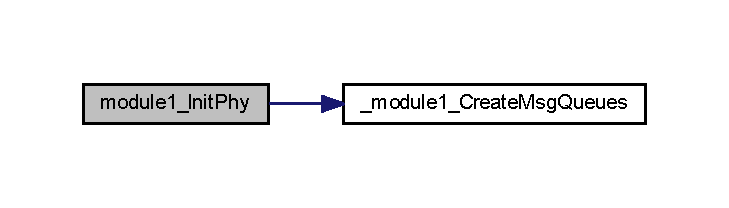
\includegraphics[width=350pt]{module_one_startup_8h_a79652bed082e520034848c4418a7b5f2_cgraph}
\end{center}
\end{figure}
\mbox{\Hypertarget{module_one_startup_8h_a33e10b04aa05e68980ba8cd27d86f51e}\label{module_one_startup_8h_a33e10b04aa05e68980ba8cd27d86f51e}} 
\index{module\+One\+Startup.\+h@{module\+One\+Startup.\+h}!module1\+\_\+\+Start\+Tasks@{module1\+\_\+\+Start\+Tasks}}
\index{module1\+\_\+\+Start\+Tasks@{module1\+\_\+\+Start\+Tasks}!module\+One\+Startup.\+h@{module\+One\+Startup.\+h}}
\subsubsection{\texorpdfstring{module1\+\_\+\+Start\+Tasks()}{module1\_StartTasks()}}
{\footnotesize\ttfamily void module1\+\_\+\+Start\+Tasks (\begin{DoxyParamCaption}\item[{void}]{ }\end{DoxyParamCaption})}



Functions for starting module 1 tasks for reading E\+TH P\+HY chip registers and retrieving test mode numbers.  S\+T\+A\+V1 13 Assembler instructions that tool can\textquotesingle{}t handle. 

Here is the call graph for this function\+:
\nopagebreak
\begin{figure}[H]
\begin{center}
\leavevmode
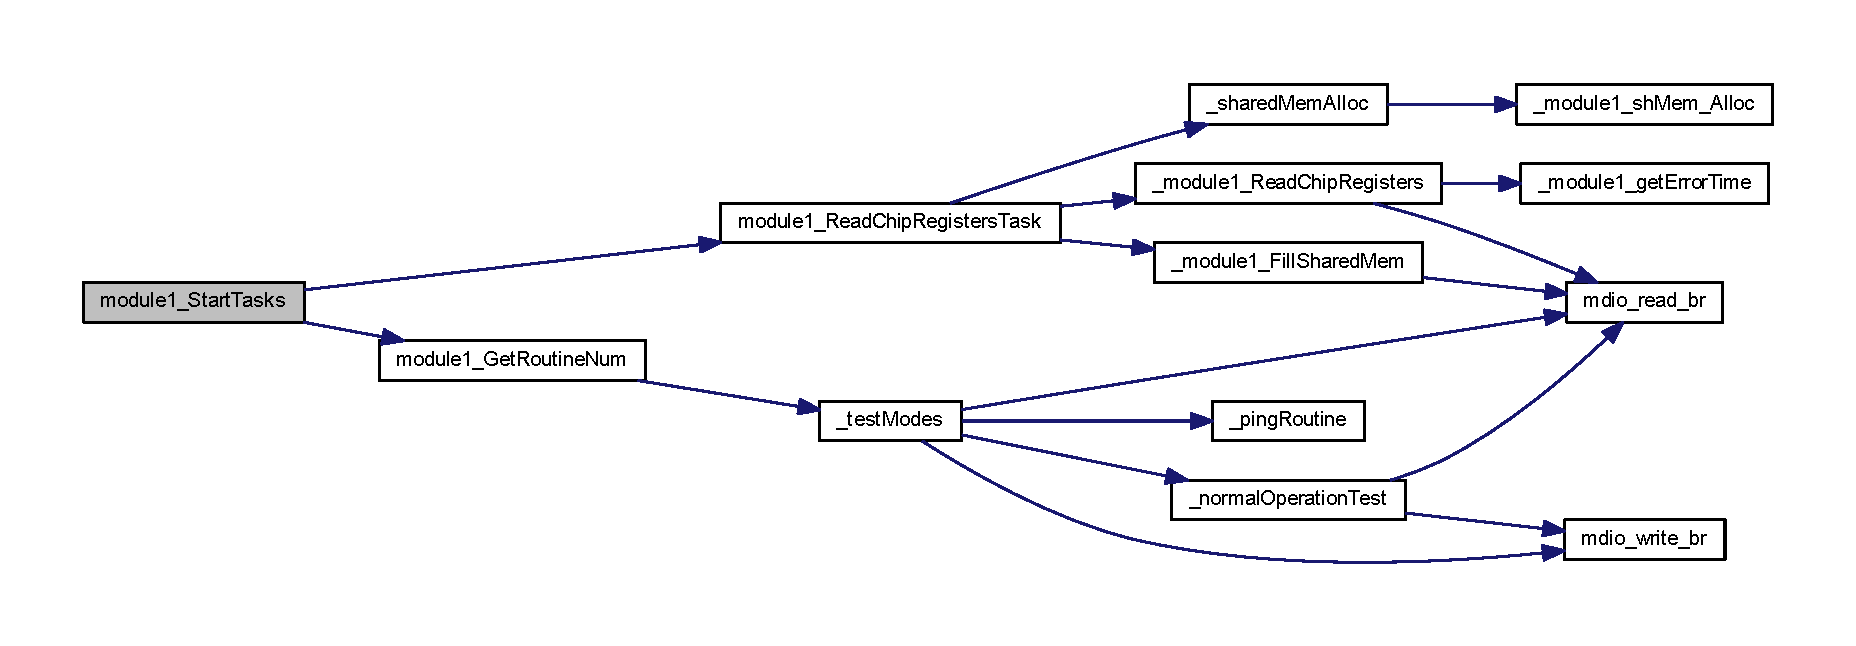
\includegraphics[width=350pt]{module_one_startup_8h_a33e10b04aa05e68980ba8cd27d86f51e_cgraph}
\end{center}
\end{figure}
\mbox{\Hypertarget{module_one_startup_8h_ae66f7a060103dcd1441b15d39845cab7}\label{module_one_startup_8h_ae66f7a060103dcd1441b15d39845cab7}} 
\index{module\+One\+Startup.\+h@{module\+One\+Startup.\+h}!rtp\+Module@{rtp\+Module}}
\index{rtp\+Module@{rtp\+Module}!module\+One\+Startup.\+h@{module\+One\+Startup.\+h}}
\subsubsection{\texorpdfstring{rtp\+Module()}{rtpModule()}}
{\footnotesize\ttfamily S\+T\+A\+T\+US rtp\+Module (\begin{DoxyParamCaption}\item[{void}]{ }\end{DoxyParamCaption})}



Initial function for starting R\+TP task in user space. 

\begin{DoxyReturn}{Returns}
OK if successful, E\+R\+R\+OR otherwise  E\+R\+R\+OR if rtp\+Spawn() function fails 
\end{DoxyReturn}

\hypertarget{module_two_communication_8c}{}\section{module\+Two\+Communication.\+c File Reference}
\label{module_two_communication_8c}\index{module\+Two\+Communication.\+c@{module\+Two\+Communication.\+c}}


Interface functions for reading shared memory and message queues with diagnostic data from module\+One.  


{\ttfamily \#include $<$vxworks.\+h$>$}\newline
{\ttfamily \#include $<$stdio.\+h$>$}\newline
{\ttfamily \#include $<$msg\+Q\+Lib\+Common.\+h$>$}\newline
{\ttfamily \#include $<$unistd.\+h$>$}\newline
{\ttfamily \#include $<$sys/fcntlcom.\+h$>$}\newline
{\ttfamily \#include $<$sys/stat.\+h$>$}\newline
{\ttfamily \#include $<$sys/mman.\+h$>$}\newline
{\ttfamily \#include \char`\"{}module\+Two\+Communication.\+h\char`\"{}}\newline
Include dependency graph for module\+Two\+Communication.\+c\+:\nopagebreak
\begin{figure}[H]
\begin{center}
\leavevmode
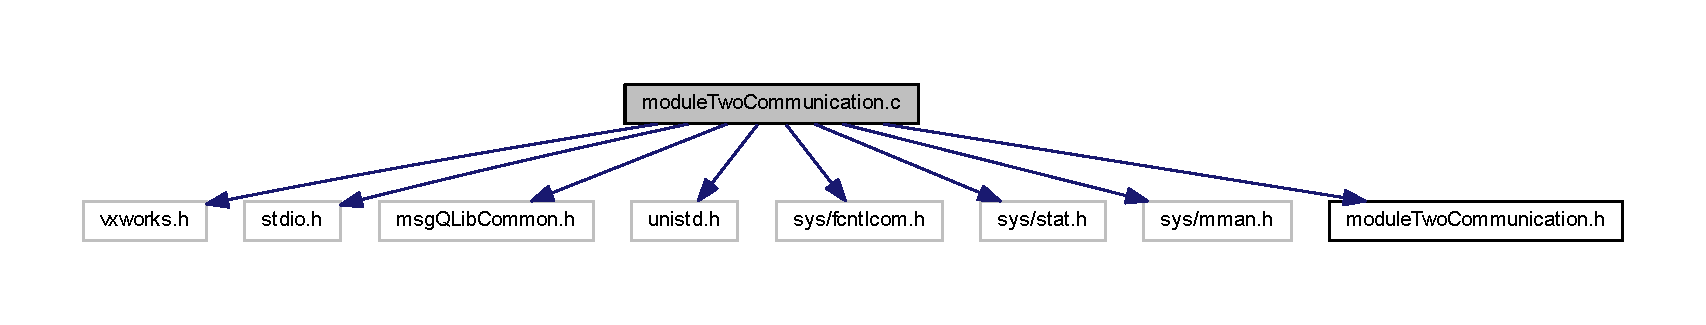
\includegraphics[width=350pt]{module_two_communication_8c__incl}
\end{center}
\end{figure}
\subsection*{Functions}
\begin{DoxyCompactItemize}
\item 
L\+O\+C\+AL void $\ast$ \mbox{\hyperlink{module_two_communication_8c_a5ad7266c95615845b7af8c438c93cf30}{\+\_\+module2\+\_\+sh\+Mem\+\_\+open}} (const char $\ast$fname, size\+\_\+t size)
\begin{DoxyCompactList}\small\item\em This function opens shared memory in module 2 and allocates it. \end{DoxyCompactList}\item 
L\+O\+C\+AL S\+T\+A\+T\+US \mbox{\hyperlink{module_two_communication_8c_adb6d8ad518b2f8d8161f37e00963d0be}{\+\_\+module2\+\_\+sh\+Mem\+\_\+\+Check}} (void)
\begin{DoxyCompactList}\small\item\em This function is used for checking if module 1 wrote correctly in shared memory. \end{DoxyCompactList}\item 
S\+T\+A\+T\+US \mbox{\hyperlink{module_two_communication_8c_ad9ebcb5d93ac5f4bc33d47aac6b88683}{\+\_\+module2\+\_\+\+Read\+Diag\+MsgQ}} (void)
\begin{DoxyCompactList}\small\item\em This function periodically reads diagnostic msgQ and shared memory. \end{DoxyCompactList}\item 
S\+T\+A\+T\+US \mbox{\hyperlink{module_two_communication_8c_a99a7dd6823d02d0f1f5d9bcfedd08fc4}{shared\+Mem\+Alloc\+\_\+module2}} (void)
\begin{DoxyCompactList}\small\item\em This function opens shared memory in module 1 and allocates it. \end{DoxyCompactList}\end{DoxyCompactItemize}
\subsection*{Variables}
\begin{DoxyCompactItemize}
\item 
\mbox{\hyperlink{__module3_8h_a1f542cc6438c66026963a340365d442a}{s\+\_\+\+D\+I\+A\+G\+\_\+\+S\+H\+M\+\_\+\+D\+A\+TA}} \mbox{\hyperlink{module_two_communication_8c_a154b6cb142b2f257168f6ce8bf4f0552}{\+\_\+diag\+\_\+shm\+\_\+struct}}
\item 
\mbox{\hyperlink{__module3_8h_a58c449f6052675fb4288c20122741cb8}{s\+\_\+\+D\+I\+A\+G\+\_\+\+D\+A\+TA}} \mbox{\hyperlink{module_two_communication_8c_ab9ff18db9b7ba52dfe985635411d0978}{\+\_\+diag\+\_\+data\+\_\+struct\+\_\+mod1}}
\item 
L\+O\+C\+AL \mbox{\hyperlink{__module3_8h_a1f542cc6438c66026963a340365d442a}{s\+\_\+\+D\+I\+A\+G\+\_\+\+S\+H\+M\+\_\+\+D\+A\+TA}} $\ast$ \mbox{\hyperlink{module_two_communication_8c_ac4998211cf8688b40208142ea2810198}{\+\_\+diag\+\_\+shm\+\_\+ptr\+\_\+check}}
\end{DoxyCompactItemize}


\subsection{Detailed Description}
Interface functions for reading shared memory and message queues with diagnostic data from module\+One. 

\mbox{\hyperlink{module_two_communication_8c}{module\+Two\+Communication.\+c}}

\begin{DoxyVersion}{Version}
\mbox{[}28-\/\+May-\/2018\mbox{]} \mbox{[}Stefan Masalusic\mbox{]} Initial creation  \mbox{[}28-\/\+May-\/2018\mbox{]} Added \+\_\+module2\+\_\+\+Read\+Diag\+MsgQ function \mbox{[}1-\/\+Jun-\/2018\mbox{]} Added shared\+Mem\+Alloc\+\_\+module2, \+\_\+module2\+\_\+sh\+Mem\+\_\+open \subsubsection*{and \+\_\+module2\+\_\+sh\+Mem\+\_\+\+Check functions }
\end{DoxyVersion}


\subsection{Function Documentation}
\mbox{\Hypertarget{module_two_communication_8c_ad9ebcb5d93ac5f4bc33d47aac6b88683}\label{module_two_communication_8c_ad9ebcb5d93ac5f4bc33d47aac6b88683}} 
\index{module\+Two\+Communication.\+c@{module\+Two\+Communication.\+c}!\+\_\+module2\+\_\+\+Read\+Diag\+MsgQ@{\+\_\+module2\+\_\+\+Read\+Diag\+MsgQ}}
\index{\+\_\+module2\+\_\+\+Read\+Diag\+MsgQ@{\+\_\+module2\+\_\+\+Read\+Diag\+MsgQ}!module\+Two\+Communication.\+c@{module\+Two\+Communication.\+c}}
\subsubsection{\texorpdfstring{\+\_\+module2\+\_\+\+Read\+Diag\+Msg\+Q()}{\_module2\_ReadDiagMsgQ()}}
{\footnotesize\ttfamily S\+T\+A\+T\+US \+\_\+module2\+\_\+\+Read\+Diag\+MsgQ (\begin{DoxyParamCaption}\item[{void}]{ }\end{DoxyParamCaption})}



This function periodically reads diagnostic msgQ and shared memory. 

\begin{DoxyReturn}{Returns}
OK if successful, E\+R\+R\+OR otherwise  E\+R\+R\+OR if opening or receiving from msg\+Queue failed 
\end{DoxyReturn}
Here is the call graph for this function\+:\nopagebreak
\begin{figure}[H]
\begin{center}
\leavevmode
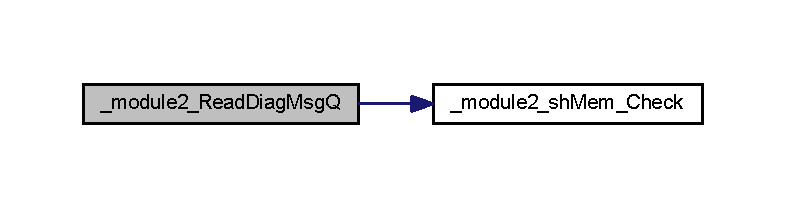
\includegraphics[width=350pt]{module_two_communication_8c_ad9ebcb5d93ac5f4bc33d47aac6b88683_cgraph}
\end{center}
\end{figure}
\mbox{\Hypertarget{module_two_communication_8c_adb6d8ad518b2f8d8161f37e00963d0be}\label{module_two_communication_8c_adb6d8ad518b2f8d8161f37e00963d0be}} 
\index{module\+Two\+Communication.\+c@{module\+Two\+Communication.\+c}!\+\_\+module2\+\_\+sh\+Mem\+\_\+\+Check@{\+\_\+module2\+\_\+sh\+Mem\+\_\+\+Check}}
\index{\+\_\+module2\+\_\+sh\+Mem\+\_\+\+Check@{\+\_\+module2\+\_\+sh\+Mem\+\_\+\+Check}!module\+Two\+Communication.\+c@{module\+Two\+Communication.\+c}}
\subsubsection{\texorpdfstring{\+\_\+module2\+\_\+sh\+Mem\+\_\+\+Check()}{\_module2\_shMem\_Check()}}
{\footnotesize\ttfamily L\+O\+C\+AL S\+T\+A\+T\+US \+\_\+module2\+\_\+sh\+Mem\+\_\+\+Check (\begin{DoxyParamCaption}\item[{void}]{ }\end{DoxyParamCaption})}



This function is used for checking if module 1 wrote correctly in shared memory. 

\begin{DoxyReturn}{Returns}
OK if successful, E\+R\+R\+OR otherwise 
\end{DoxyReturn}
\mbox{\Hypertarget{module_two_communication_8c_a5ad7266c95615845b7af8c438c93cf30}\label{module_two_communication_8c_a5ad7266c95615845b7af8c438c93cf30}} 
\index{module\+Two\+Communication.\+c@{module\+Two\+Communication.\+c}!\+\_\+module2\+\_\+sh\+Mem\+\_\+open@{\+\_\+module2\+\_\+sh\+Mem\+\_\+open}}
\index{\+\_\+module2\+\_\+sh\+Mem\+\_\+open@{\+\_\+module2\+\_\+sh\+Mem\+\_\+open}!module\+Two\+Communication.\+c@{module\+Two\+Communication.\+c}}
\subsubsection{\texorpdfstring{\+\_\+module2\+\_\+sh\+Mem\+\_\+open()}{\_module2\_shMem\_open()}}
{\footnotesize\ttfamily L\+O\+C\+AL void $\ast$ \+\_\+module2\+\_\+sh\+Mem\+\_\+open (\begin{DoxyParamCaption}\item[{const char $\ast$}]{fname,  }\item[{size\+\_\+t}]{size }\end{DoxyParamCaption})}



This function opens shared memory in module 2 and allocates it. 


\begin{DoxyParams}{Parameters}
{\em fname} & Name of shared memory \\
\hline
{\em size} & Size of shared memory \\
\hline
\end{DoxyParams}
\begin{DoxyReturn}{Returns}
Pointer to allocated shared memory 
\end{DoxyReturn}
\mbox{\Hypertarget{module_two_communication_8c_a99a7dd6823d02d0f1f5d9bcfedd08fc4}\label{module_two_communication_8c_a99a7dd6823d02d0f1f5d9bcfedd08fc4}} 
\index{module\+Two\+Communication.\+c@{module\+Two\+Communication.\+c}!shared\+Mem\+Alloc\+\_\+module2@{shared\+Mem\+Alloc\+\_\+module2}}
\index{shared\+Mem\+Alloc\+\_\+module2@{shared\+Mem\+Alloc\+\_\+module2}!module\+Two\+Communication.\+c@{module\+Two\+Communication.\+c}}
\subsubsection{\texorpdfstring{shared\+Mem\+Alloc\+\_\+module2()}{sharedMemAlloc\_module2()}}
{\footnotesize\ttfamily S\+T\+A\+T\+US shared\+Mem\+Alloc\+\_\+module2 (\begin{DoxyParamCaption}\item[{void}]{ }\end{DoxyParamCaption})}



This function opens shared memory in module 1 and allocates it. 

\begin{DoxyReturn}{Returns}
OK if successful, E\+R\+R\+OR otherwise  E\+R\+R\+OR if opening shared memory failed 
\end{DoxyReturn}
Here is the call graph for this function\+:\nopagebreak
\begin{figure}[H]
\begin{center}
\leavevmode
\includegraphics[width=350pt]{module_two_communication_8c_a99a7dd6823d02d0f1f5d9bcfedd08fc4_cgraph}
\end{center}
\end{figure}


\subsection{Variable Documentation}
\mbox{\Hypertarget{module_two_communication_8c_ab9ff18db9b7ba52dfe985635411d0978}\label{module_two_communication_8c_ab9ff18db9b7ba52dfe985635411d0978}} 
\index{module\+Two\+Communication.\+c@{module\+Two\+Communication.\+c}!\+\_\+diag\+\_\+data\+\_\+struct\+\_\+mod1@{\+\_\+diag\+\_\+data\+\_\+struct\+\_\+mod1}}
\index{\+\_\+diag\+\_\+data\+\_\+struct\+\_\+mod1@{\+\_\+diag\+\_\+data\+\_\+struct\+\_\+mod1}!module\+Two\+Communication.\+c@{module\+Two\+Communication.\+c}}
\subsubsection{\texorpdfstring{\+\_\+diag\+\_\+data\+\_\+struct\+\_\+mod1}{\_diag\_data\_struct\_mod1}}
{\footnotesize\ttfamily \mbox{\hyperlink{__module3_8h_a58c449f6052675fb4288c20122741cb8}{s\+\_\+\+D\+I\+A\+G\+\_\+\+D\+A\+TA}} \+\_\+diag\+\_\+data\+\_\+struct\+\_\+mod1}

\mbox{\Hypertarget{module_two_communication_8c_ac4998211cf8688b40208142ea2810198}\label{module_two_communication_8c_ac4998211cf8688b40208142ea2810198}} 
\index{module\+Two\+Communication.\+c@{module\+Two\+Communication.\+c}!\+\_\+diag\+\_\+shm\+\_\+ptr\+\_\+check@{\+\_\+diag\+\_\+shm\+\_\+ptr\+\_\+check}}
\index{\+\_\+diag\+\_\+shm\+\_\+ptr\+\_\+check@{\+\_\+diag\+\_\+shm\+\_\+ptr\+\_\+check}!module\+Two\+Communication.\+c@{module\+Two\+Communication.\+c}}
\subsubsection{\texorpdfstring{\+\_\+diag\+\_\+shm\+\_\+ptr\+\_\+check}{\_diag\_shm\_ptr\_check}}
{\footnotesize\ttfamily L\+O\+C\+AL \mbox{\hyperlink{__module3_8h_a1f542cc6438c66026963a340365d442a}{s\+\_\+\+D\+I\+A\+G\+\_\+\+S\+H\+M\+\_\+\+D\+A\+TA}}$\ast$ \+\_\+diag\+\_\+shm\+\_\+ptr\+\_\+check}

\mbox{\Hypertarget{module_two_communication_8c_a154b6cb142b2f257168f6ce8bf4f0552}\label{module_two_communication_8c_a154b6cb142b2f257168f6ce8bf4f0552}} 
\index{module\+Two\+Communication.\+c@{module\+Two\+Communication.\+c}!\+\_\+diag\+\_\+shm\+\_\+struct@{\+\_\+diag\+\_\+shm\+\_\+struct}}
\index{\+\_\+diag\+\_\+shm\+\_\+struct@{\+\_\+diag\+\_\+shm\+\_\+struct}!module\+Two\+Communication.\+c@{module\+Two\+Communication.\+c}}
\subsubsection{\texorpdfstring{\+\_\+diag\+\_\+shm\+\_\+struct}{\_diag\_shm\_struct}}
{\footnotesize\ttfamily \mbox{\hyperlink{__module3_8h_a1f542cc6438c66026963a340365d442a}{s\+\_\+\+D\+I\+A\+G\+\_\+\+S\+H\+M\+\_\+\+D\+A\+TA}} \+\_\+diag\+\_\+shm\+\_\+struct}


\hypertarget{module_two_communication_8h}{}\section{module\+Two\+Communication.\+h File Reference}
\label{module_two_communication_8h}\index{module\+Two\+Communication.\+h@{module\+Two\+Communication.\+h}}


Header file for \mbox{\hyperlink{module_two_communication_8c}{module\+Two\+Communication.\+c}}.  


This graph shows which files directly or indirectly include this file\+:\nopagebreak
\begin{figure}[H]
\begin{center}
\leavevmode
\includegraphics[width=350pt]{module_two_communication_8h__dep__incl}
\end{center}
\end{figure}
\subsection*{Classes}
\begin{DoxyCompactItemize}
\item 
struct \mbox{\hyperlink{structerror_struct}{error\+Struct}}
\item 
struct \mbox{\hyperlink{structdiagnostic_data_msg_q}{diagnostic\+Data\+MsgQ}}
\item 
struct \mbox{\hyperlink{structdiagnostic_data_sh_m}{diagnostic\+Data\+ShM}}
\end{DoxyCompactItemize}
\subsection*{Macros}
\begin{DoxyCompactItemize}
\item 
\#define \mbox{\hyperlink{module_two_communication_8h_a530f11a96e508d171d28564c8dc20942}{N\+U\+L\+L\+\_\+\+P\+TR}}~(void $\ast$) (0)
\item 
\#define \mbox{\hyperlink{module_two_communication_8h_ad89c5a76e69b781c64de110635a95d1d}{S\+H\+\_\+\+M\+E\+M\+\_\+\+N\+A\+ME}}~\char`\"{}/sh\+Mem\+Module1to2\char`\"{}
\item 
\#define \mbox{\hyperlink{module_two_communication_8h_aa24597a54a085c6c2c33b64138f09eff}{M\+A\+X\+\_\+\+M\+SG}}~(2\+U)
\end{DoxyCompactItemize}
\subsection*{Typedefs}
\begin{DoxyCompactItemize}
\item 
typedef struct \mbox{\hyperlink{structerror_struct}{error\+Struct}} \mbox{\hyperlink{module_two_communication_8h_aed782b3a5727361a6b656be14d539f9c}{s\+\_\+\+E\+R\+R\+O\+RS}}
\item 
typedef struct \mbox{\hyperlink{structdiagnostic_data_msg_q}{diagnostic\+Data\+MsgQ}} \mbox{\hyperlink{module_two_communication_8h_a58c449f6052675fb4288c20122741cb8}{s\+\_\+\+D\+I\+A\+G\+\_\+\+D\+A\+TA}}
\item 
typedef struct \mbox{\hyperlink{structdiagnostic_data_sh_m}{diagnostic\+Data\+ShM}} \mbox{\hyperlink{module_two_communication_8h_a1f542cc6438c66026963a340365d442a}{s\+\_\+\+D\+I\+A\+G\+\_\+\+S\+H\+M\+\_\+\+D\+A\+TA}}
\end{DoxyCompactItemize}
\subsection*{Functions}
\begin{DoxyCompactItemize}
\item 
S\+T\+A\+T\+US \mbox{\hyperlink{module_two_communication_8h_ad9ebcb5d93ac5f4bc33d47aac6b88683}{\+\_\+module2\+\_\+\+Read\+Diag\+MsgQ}} (void)
\begin{DoxyCompactList}\small\item\em This function periodically reads diagnostic msgQ and shared memory. \end{DoxyCompactList}\item 
S\+T\+A\+T\+US \mbox{\hyperlink{module_two_communication_8h_a99a7dd6823d02d0f1f5d9bcfedd08fc4}{shared\+Mem\+Alloc\+\_\+module2}} (void)
\begin{DoxyCompactList}\small\item\em This function opens shared memory in module 1 and allocates it. \end{DoxyCompactList}\end{DoxyCompactItemize}
\subsection*{Variables}
\begin{DoxyCompactItemize}
\item 
\mbox{\hyperlink{__module3_8h_a1f542cc6438c66026963a340365d442a}{s\+\_\+\+D\+I\+A\+G\+\_\+\+S\+H\+M\+\_\+\+D\+A\+TA}} \mbox{\hyperlink{module_two_communication_8h_a154b6cb142b2f257168f6ce8bf4f0552}{\+\_\+diag\+\_\+shm\+\_\+struct}}
\item 
\mbox{\hyperlink{__module3_8h_a58c449f6052675fb4288c20122741cb8}{s\+\_\+\+D\+I\+A\+G\+\_\+\+D\+A\+TA}} \mbox{\hyperlink{module_two_communication_8h_ab9ff18db9b7ba52dfe985635411d0978}{\+\_\+diag\+\_\+data\+\_\+struct\+\_\+mod1}}
\end{DoxyCompactItemize}


\subsection{Detailed Description}
Header file for \mbox{\hyperlink{module_two_communication_8c}{module\+Two\+Communication.\+c}}. 

\mbox{\hyperlink{module_two_communication_8h}{module\+Two\+Communication.\+h}}

\begin{DoxyVersion}{Version}
\mbox{[}28-\/\+May-\/2018\mbox{]} \mbox{[}Stefan Masalusic\mbox{]} Initial creation  \mbox{[}28-\/\+May-\/2018\mbox{]} Defined structures \mbox{[}7-\/\+Jun-\/2018\mbox{]} Added function descriptions \subsubsection*{\mbox{[}09-\/\+Jul-\/2018\mbox{]} Added macros }
\end{DoxyVersion}


\subsection{Macro Definition Documentation}
\mbox{\Hypertarget{module_two_communication_8h_aa24597a54a085c6c2c33b64138f09eff}\label{module_two_communication_8h_aa24597a54a085c6c2c33b64138f09eff}} 
\index{module\+Two\+Communication.\+h@{module\+Two\+Communication.\+h}!M\+A\+X\+\_\+\+M\+SG@{M\+A\+X\+\_\+\+M\+SG}}
\index{M\+A\+X\+\_\+\+M\+SG@{M\+A\+X\+\_\+\+M\+SG}!module\+Two\+Communication.\+h@{module\+Two\+Communication.\+h}}
\subsubsection{\texorpdfstring{M\+A\+X\+\_\+\+M\+SG}{MAX\_MSG}}
{\footnotesize\ttfamily \#define M\+A\+X\+\_\+\+M\+SG~(2\+U)}

\mbox{\Hypertarget{module_two_communication_8h_a530f11a96e508d171d28564c8dc20942}\label{module_two_communication_8h_a530f11a96e508d171d28564c8dc20942}} 
\index{module\+Two\+Communication.\+h@{module\+Two\+Communication.\+h}!N\+U\+L\+L\+\_\+\+P\+TR@{N\+U\+L\+L\+\_\+\+P\+TR}}
\index{N\+U\+L\+L\+\_\+\+P\+TR@{N\+U\+L\+L\+\_\+\+P\+TR}!module\+Two\+Communication.\+h@{module\+Two\+Communication.\+h}}
\subsubsection{\texorpdfstring{N\+U\+L\+L\+\_\+\+P\+TR}{NULL\_PTR}}
{\footnotesize\ttfamily \#define N\+U\+L\+L\+\_\+\+P\+TR~(void $\ast$) (0)}

\mbox{\Hypertarget{module_two_communication_8h_ad89c5a76e69b781c64de110635a95d1d}\label{module_two_communication_8h_ad89c5a76e69b781c64de110635a95d1d}} 
\index{module\+Two\+Communication.\+h@{module\+Two\+Communication.\+h}!S\+H\+\_\+\+M\+E\+M\+\_\+\+N\+A\+ME@{S\+H\+\_\+\+M\+E\+M\+\_\+\+N\+A\+ME}}
\index{S\+H\+\_\+\+M\+E\+M\+\_\+\+N\+A\+ME@{S\+H\+\_\+\+M\+E\+M\+\_\+\+N\+A\+ME}!module\+Two\+Communication.\+h@{module\+Two\+Communication.\+h}}
\subsubsection{\texorpdfstring{S\+H\+\_\+\+M\+E\+M\+\_\+\+N\+A\+ME}{SH\_MEM\_NAME}}
{\footnotesize\ttfamily \#define S\+H\+\_\+\+M\+E\+M\+\_\+\+N\+A\+ME~\char`\"{}/sh\+Mem\+Module1to2\char`\"{}}



\subsection{Typedef Documentation}
\mbox{\Hypertarget{module_two_communication_8h_a58c449f6052675fb4288c20122741cb8}\label{module_two_communication_8h_a58c449f6052675fb4288c20122741cb8}} 
\index{module\+Two\+Communication.\+h@{module\+Two\+Communication.\+h}!s\+\_\+\+D\+I\+A\+G\+\_\+\+D\+A\+TA@{s\+\_\+\+D\+I\+A\+G\+\_\+\+D\+A\+TA}}
\index{s\+\_\+\+D\+I\+A\+G\+\_\+\+D\+A\+TA@{s\+\_\+\+D\+I\+A\+G\+\_\+\+D\+A\+TA}!module\+Two\+Communication.\+h@{module\+Two\+Communication.\+h}}
\subsubsection{\texorpdfstring{s\+\_\+\+D\+I\+A\+G\+\_\+\+D\+A\+TA}{s\_DIAG\_DATA}}
{\footnotesize\ttfamily typedef struct \mbox{\hyperlink{structdiagnostic_data_msg_q}{diagnostic\+Data\+MsgQ}}  \mbox{\hyperlink{__module3_8h_a58c449f6052675fb4288c20122741cb8}{s\+\_\+\+D\+I\+A\+G\+\_\+\+D\+A\+TA}}}

\mbox{\Hypertarget{module_two_communication_8h_a1f542cc6438c66026963a340365d442a}\label{module_two_communication_8h_a1f542cc6438c66026963a340365d442a}} 
\index{module\+Two\+Communication.\+h@{module\+Two\+Communication.\+h}!s\+\_\+\+D\+I\+A\+G\+\_\+\+S\+H\+M\+\_\+\+D\+A\+TA@{s\+\_\+\+D\+I\+A\+G\+\_\+\+S\+H\+M\+\_\+\+D\+A\+TA}}
\index{s\+\_\+\+D\+I\+A\+G\+\_\+\+S\+H\+M\+\_\+\+D\+A\+TA@{s\+\_\+\+D\+I\+A\+G\+\_\+\+S\+H\+M\+\_\+\+D\+A\+TA}!module\+Two\+Communication.\+h@{module\+Two\+Communication.\+h}}
\subsubsection{\texorpdfstring{s\+\_\+\+D\+I\+A\+G\+\_\+\+S\+H\+M\+\_\+\+D\+A\+TA}{s\_DIAG\_SHM\_DATA}}
{\footnotesize\ttfamily typedef struct \mbox{\hyperlink{structdiagnostic_data_sh_m}{diagnostic\+Data\+ShM}}  \mbox{\hyperlink{__module3_8h_a1f542cc6438c66026963a340365d442a}{s\+\_\+\+D\+I\+A\+G\+\_\+\+S\+H\+M\+\_\+\+D\+A\+TA}}}

\mbox{\Hypertarget{module_two_communication_8h_aed782b3a5727361a6b656be14d539f9c}\label{module_two_communication_8h_aed782b3a5727361a6b656be14d539f9c}} 
\index{module\+Two\+Communication.\+h@{module\+Two\+Communication.\+h}!s\+\_\+\+E\+R\+R\+O\+RS@{s\+\_\+\+E\+R\+R\+O\+RS}}
\index{s\+\_\+\+E\+R\+R\+O\+RS@{s\+\_\+\+E\+R\+R\+O\+RS}!module\+Two\+Communication.\+h@{module\+Two\+Communication.\+h}}
\subsubsection{\texorpdfstring{s\+\_\+\+E\+R\+R\+O\+RS}{s\_ERRORS}}
{\footnotesize\ttfamily typedef struct \mbox{\hyperlink{structerror_struct}{error\+Struct}} \mbox{\hyperlink{__module3_8h_aed782b3a5727361a6b656be14d539f9c}{s\+\_\+\+E\+R\+R\+O\+RS}}}



\subsection{Function Documentation}
\mbox{\Hypertarget{module_two_communication_8h_ad9ebcb5d93ac5f4bc33d47aac6b88683}\label{module_two_communication_8h_ad9ebcb5d93ac5f4bc33d47aac6b88683}} 
\index{module\+Two\+Communication.\+h@{module\+Two\+Communication.\+h}!\+\_\+module2\+\_\+\+Read\+Diag\+MsgQ@{\+\_\+module2\+\_\+\+Read\+Diag\+MsgQ}}
\index{\+\_\+module2\+\_\+\+Read\+Diag\+MsgQ@{\+\_\+module2\+\_\+\+Read\+Diag\+MsgQ}!module\+Two\+Communication.\+h@{module\+Two\+Communication.\+h}}
\subsubsection{\texorpdfstring{\+\_\+module2\+\_\+\+Read\+Diag\+Msg\+Q()}{\_module2\_ReadDiagMsgQ()}}
{\footnotesize\ttfamily S\+T\+A\+T\+US \+\_\+module2\+\_\+\+Read\+Diag\+MsgQ (\begin{DoxyParamCaption}\item[{void}]{ }\end{DoxyParamCaption})}



This function periodically reads diagnostic msgQ and shared memory. 

\begin{DoxyReturn}{Returns}
OK if successful, E\+R\+R\+OR otherwise  E\+R\+R\+OR if opening or receiving from msg\+Queue failed 
\end{DoxyReturn}
Here is the call graph for this function\+:\nopagebreak
\begin{figure}[H]
\begin{center}
\leavevmode
\includegraphics[width=350pt]{module_two_communication_8h_ad9ebcb5d93ac5f4bc33d47aac6b88683_cgraph}
\end{center}
\end{figure}
\mbox{\Hypertarget{module_two_communication_8h_a99a7dd6823d02d0f1f5d9bcfedd08fc4}\label{module_two_communication_8h_a99a7dd6823d02d0f1f5d9bcfedd08fc4}} 
\index{module\+Two\+Communication.\+h@{module\+Two\+Communication.\+h}!shared\+Mem\+Alloc\+\_\+module2@{shared\+Mem\+Alloc\+\_\+module2}}
\index{shared\+Mem\+Alloc\+\_\+module2@{shared\+Mem\+Alloc\+\_\+module2}!module\+Two\+Communication.\+h@{module\+Two\+Communication.\+h}}
\subsubsection{\texorpdfstring{shared\+Mem\+Alloc\+\_\+module2()}{sharedMemAlloc\_module2()}}
{\footnotesize\ttfamily S\+T\+A\+T\+US shared\+Mem\+Alloc\+\_\+module2 (\begin{DoxyParamCaption}\item[{void}]{ }\end{DoxyParamCaption})}



This function opens shared memory in module 1 and allocates it. 

\begin{DoxyReturn}{Returns}
OK if successful, E\+R\+R\+OR otherwise  E\+R\+R\+OR if opening shared memory failed 
\end{DoxyReturn}
Here is the call graph for this function\+:\nopagebreak
\begin{figure}[H]
\begin{center}
\leavevmode
\includegraphics[width=350pt]{module_two_communication_8h_a99a7dd6823d02d0f1f5d9bcfedd08fc4_cgraph}
\end{center}
\end{figure}


\subsection{Variable Documentation}
\mbox{\Hypertarget{module_two_communication_8h_ab9ff18db9b7ba52dfe985635411d0978}\label{module_two_communication_8h_ab9ff18db9b7ba52dfe985635411d0978}} 
\index{module\+Two\+Communication.\+h@{module\+Two\+Communication.\+h}!\+\_\+diag\+\_\+data\+\_\+struct\+\_\+mod1@{\+\_\+diag\+\_\+data\+\_\+struct\+\_\+mod1}}
\index{\+\_\+diag\+\_\+data\+\_\+struct\+\_\+mod1@{\+\_\+diag\+\_\+data\+\_\+struct\+\_\+mod1}!module\+Two\+Communication.\+h@{module\+Two\+Communication.\+h}}
\subsubsection{\texorpdfstring{\+\_\+diag\+\_\+data\+\_\+struct\+\_\+mod1}{\_diag\_data\_struct\_mod1}}
{\footnotesize\ttfamily \mbox{\hyperlink{__module3_8h_a58c449f6052675fb4288c20122741cb8}{s\+\_\+\+D\+I\+A\+G\+\_\+\+D\+A\+TA}} \+\_\+diag\+\_\+data\+\_\+struct\+\_\+mod1}

\mbox{\Hypertarget{module_two_communication_8h_a154b6cb142b2f257168f6ce8bf4f0552}\label{module_two_communication_8h_a154b6cb142b2f257168f6ce8bf4f0552}} 
\index{module\+Two\+Communication.\+h@{module\+Two\+Communication.\+h}!\+\_\+diag\+\_\+shm\+\_\+struct@{\+\_\+diag\+\_\+shm\+\_\+struct}}
\index{\+\_\+diag\+\_\+shm\+\_\+struct@{\+\_\+diag\+\_\+shm\+\_\+struct}!module\+Two\+Communication.\+h@{module\+Two\+Communication.\+h}}
\subsubsection{\texorpdfstring{\+\_\+diag\+\_\+shm\+\_\+struct}{\_diag\_shm\_struct}}
{\footnotesize\ttfamily \mbox{\hyperlink{__module3_8h_a1f542cc6438c66026963a340365d442a}{s\+\_\+\+D\+I\+A\+G\+\_\+\+S\+H\+M\+\_\+\+D\+A\+TA}} \+\_\+diag\+\_\+shm\+\_\+struct}


\hypertarget{module_two_file_sending_8c}{}\section{module\+Two\+File\+Sending.\+c File Reference}
\label{module_two_file_sending_8c}\index{module\+Two\+File\+Sending.\+c@{module\+Two\+File\+Sending.\+c}}


Functions that handle file sending to PC side.  


{\ttfamily \#include $<$vxworks.\+h$>$}\newline
{\ttfamily \#include $<$stdio.\+h$>$}\newline
{\ttfamily \#include $<$dirent.\+h$>$}\newline
{\ttfamily \#include $<$sock\+Lib.\+h$>$}\newline
{\ttfamily \#include $<$string.\+h$>$}\newline
{\ttfamily \#include $<$errno.\+h$>$}\newline
{\ttfamily \#include $<$time.\+h$>$}\newline
{\ttfamily \#include \char`\"{}module\+Two\+Server.\+h\char`\"{}}\newline
{\ttfamily \#include \char`\"{}module\+Two\+Handle\+Routines.\+h\char`\"{}}\newline
{\ttfamily \#include \char`\"{}module\+Two\+File\+Sending.\+h\char`\"{}}\newline
Include dependency graph for module\+Two\+File\+Sending.\+c\+:
\nopagebreak
\begin{figure}[H]
\begin{center}
\leavevmode
\includegraphics[width=350pt]{module_two_file_sending_8c__incl}
\end{center}
\end{figure}
\subsection*{Functions}
\begin{DoxyCompactItemize}
\item 
L\+O\+C\+AL void \mbox{\hyperlink{module_two_file_sending_8c_a171d25e73f48edc57c8e207c7185693f}{\+\_\+process\+File\+Name}} (char fs\+\_\+name\mbox{[}$\,$\mbox{]})
\begin{DoxyCompactList}\small\item\em This function prepares and send filename to PC via socket. \end{DoxyCompactList}\item 
L\+O\+C\+AL void \mbox{\hyperlink{module_two_file_sending_8c_aa76180fc2669d77f3ea52e452e97ff58}{\+\_\+process\+File\+Size}} (void)
\begin{DoxyCompactList}\small\item\em This function prepares and send filesize to PC via socket.  S\+T\+A\+V1 10 Required for correct implementation of file sending. \end{DoxyCompactList}\item 
L\+O\+C\+AL void \mbox{\hyperlink{module_two_file_sending_8c_ad079ec43554602f3e23e69e4b7c666fb}{\+\_\+process\+File\+Sending}} (void)
\begin{DoxyCompactList}\small\item\em This function sends file data through socket.  S\+T\+C\+AL 10 Required for correct implementation of file sending. \end{DoxyCompactList}\item 
L\+O\+C\+AL void \mbox{\hyperlink{module_two_file_sending_8c_a0817368c3c0a7b326aaa73ce4789c954}{\+\_\+send\+File}} (char fs\+\_\+name\mbox{[}$\,$\mbox{]})
\begin{DoxyCompactList}\small\item\em This function sends file to PC. \end{DoxyCompactList}\item 
void \mbox{\hyperlink{module_two_file_sending_8c_adb58ea2632a87ebf50ddc6dc9737a94a}{upload\+File}} (void)
\begin{DoxyCompactList}\small\item\em This function sends number of files that are going to be sent through socket and calls \mbox{\hyperlink{module_two_file_sending_8c_a0817368c3c0a7b326aaa73ce4789c954}{\+\_\+send\+File()}}. \end{DoxyCompactList}\end{DoxyCompactItemize}
\subsection*{Variables}
\begin{DoxyCompactItemize}
\item 
L\+O\+C\+AL char \mbox{\hyperlink{module_two_file_sending_8c_aa747251104a2854d1373be8a48b58b90}{\+\_\+temp\+Dir}} \mbox{[}\mbox{\hyperlink{module_two_server_8h_ad974fe981249f5e84fbf1683b012c9f8}{B\+U\+F\+L\+EN}}\mbox{]}
\item 
L\+O\+C\+AL F\+I\+LE $\ast$ \mbox{\hyperlink{module_two_file_sending_8c_abab72f2ea0fac72c01be486949902537}{\+\_\+fs}}
\end{DoxyCompactItemize}


\subsection{Detailed Description}
Functions that handle file sending to PC side. 

\mbox{\hyperlink{module_two_file_sending_8c}{module\+Two\+File\+Sending.\+c}}

\begin{DoxyVersion}{Version}
\mbox{[}8-\/\+Jun-\/2018\mbox{]} \mbox{[}Stefan Masalusic\mbox{]} Initial creation  \subsubsection*{\mbox{[}11-\/\+Jun-\/2018\mbox{]} Finished all functions }
\end{DoxyVersion}


\subsection{Function Documentation}
\mbox{\Hypertarget{module_two_file_sending_8c_a171d25e73f48edc57c8e207c7185693f}\label{module_two_file_sending_8c_a171d25e73f48edc57c8e207c7185693f}} 
\index{module\+Two\+File\+Sending.\+c@{module\+Two\+File\+Sending.\+c}!\+\_\+process\+File\+Name@{\+\_\+process\+File\+Name}}
\index{\+\_\+process\+File\+Name@{\+\_\+process\+File\+Name}!module\+Two\+File\+Sending.\+c@{module\+Two\+File\+Sending.\+c}}
\subsubsection{\texorpdfstring{\+\_\+process\+File\+Name()}{\_processFileName()}}
{\footnotesize\ttfamily L\+O\+C\+AL void \+\_\+process\+File\+Name (\begin{DoxyParamCaption}\item[{char}]{fs\+\_\+name\mbox{[}$\,$\mbox{]} }\end{DoxyParamCaption})}



This function prepares and send filename to PC via socket. 


\begin{DoxyParams}{Parameters}
{\em fs\+\_\+name\mbox{[}$\,$\mbox{]}} & Name of file to be sent \\
\hline
\end{DoxyParams}
\mbox{\Hypertarget{module_two_file_sending_8c_ad079ec43554602f3e23e69e4b7c666fb}\label{module_two_file_sending_8c_ad079ec43554602f3e23e69e4b7c666fb}} 
\index{module\+Two\+File\+Sending.\+c@{module\+Two\+File\+Sending.\+c}!\+\_\+process\+File\+Sending@{\+\_\+process\+File\+Sending}}
\index{\+\_\+process\+File\+Sending@{\+\_\+process\+File\+Sending}!module\+Two\+File\+Sending.\+c@{module\+Two\+File\+Sending.\+c}}
\subsubsection{\texorpdfstring{\+\_\+process\+File\+Sending()}{\_processFileSending()}}
{\footnotesize\ttfamily L\+O\+C\+AL void \+\_\+process\+File\+Sending (\begin{DoxyParamCaption}\item[{void}]{ }\end{DoxyParamCaption})}



This function sends file data through socket.  S\+T\+C\+AL 10 Required for correct implementation of file sending. 

\mbox{\Hypertarget{module_two_file_sending_8c_aa76180fc2669d77f3ea52e452e97ff58}\label{module_two_file_sending_8c_aa76180fc2669d77f3ea52e452e97ff58}} 
\index{module\+Two\+File\+Sending.\+c@{module\+Two\+File\+Sending.\+c}!\+\_\+process\+File\+Size@{\+\_\+process\+File\+Size}}
\index{\+\_\+process\+File\+Size@{\+\_\+process\+File\+Size}!module\+Two\+File\+Sending.\+c@{module\+Two\+File\+Sending.\+c}}
\subsubsection{\texorpdfstring{\+\_\+process\+File\+Size()}{\_processFileSize()}}
{\footnotesize\ttfamily L\+O\+C\+AL void \+\_\+process\+File\+Size (\begin{DoxyParamCaption}\item[{void}]{ }\end{DoxyParamCaption})}



This function prepares and send filesize to PC via socket.  S\+T\+A\+V1 10 Required for correct implementation of file sending. 

\mbox{\Hypertarget{module_two_file_sending_8c_a0817368c3c0a7b326aaa73ce4789c954}\label{module_two_file_sending_8c_a0817368c3c0a7b326aaa73ce4789c954}} 
\index{module\+Two\+File\+Sending.\+c@{module\+Two\+File\+Sending.\+c}!\+\_\+send\+File@{\+\_\+send\+File}}
\index{\+\_\+send\+File@{\+\_\+send\+File}!module\+Two\+File\+Sending.\+c@{module\+Two\+File\+Sending.\+c}}
\subsubsection{\texorpdfstring{\+\_\+send\+File()}{\_sendFile()}}
{\footnotesize\ttfamily L\+O\+C\+AL void \+\_\+send\+File (\begin{DoxyParamCaption}\item[{char}]{fs\+\_\+name\mbox{[}$\,$\mbox{]} }\end{DoxyParamCaption})}



This function sends file to PC. 


\begin{DoxyParams}{Parameters}
{\em fs\+\_\+name\mbox{[}$\,$\mbox{]}} & Name of file to be sent with full path \\
\hline
\end{DoxyParams}
Here is the call graph for this function\+:
\nopagebreak
\begin{figure}[H]
\begin{center}
\leavevmode
\includegraphics[width=282pt]{module_two_file_sending_8c_a0817368c3c0a7b326aaa73ce4789c954_cgraph}
\end{center}
\end{figure}
\mbox{\Hypertarget{module_two_file_sending_8c_adb58ea2632a87ebf50ddc6dc9737a94a}\label{module_two_file_sending_8c_adb58ea2632a87ebf50ddc6dc9737a94a}} 
\index{module\+Two\+File\+Sending.\+c@{module\+Two\+File\+Sending.\+c}!upload\+File@{upload\+File}}
\index{upload\+File@{upload\+File}!module\+Two\+File\+Sending.\+c@{module\+Two\+File\+Sending.\+c}}
\subsubsection{\texorpdfstring{upload\+File()}{uploadFile()}}
{\footnotesize\ttfamily void upload\+File (\begin{DoxyParamCaption}\item[{void}]{ }\end{DoxyParamCaption})}



This function sends number of files that are going to be sent through socket and calls \mbox{\hyperlink{module_two_file_sending_8c_a0817368c3c0a7b326aaa73ce4789c954}{\+\_\+send\+File()}}. 

Here is the call graph for this function\+:
\nopagebreak
\begin{figure}[H]
\begin{center}
\leavevmode
\includegraphics[width=350pt]{module_two_file_sending_8c_adb58ea2632a87ebf50ddc6dc9737a94a_cgraph}
\end{center}
\end{figure}


\subsection{Variable Documentation}
\mbox{\Hypertarget{module_two_file_sending_8c_abab72f2ea0fac72c01be486949902537}\label{module_two_file_sending_8c_abab72f2ea0fac72c01be486949902537}} 
\index{module\+Two\+File\+Sending.\+c@{module\+Two\+File\+Sending.\+c}!\+\_\+fs@{\+\_\+fs}}
\index{\+\_\+fs@{\+\_\+fs}!module\+Two\+File\+Sending.\+c@{module\+Two\+File\+Sending.\+c}}
\subsubsection{\texorpdfstring{\+\_\+fs}{\_fs}}
{\footnotesize\ttfamily L\+O\+C\+AL F\+I\+LE$\ast$ \+\_\+fs}

\mbox{\Hypertarget{module_two_file_sending_8c_aa747251104a2854d1373be8a48b58b90}\label{module_two_file_sending_8c_aa747251104a2854d1373be8a48b58b90}} 
\index{module\+Two\+File\+Sending.\+c@{module\+Two\+File\+Sending.\+c}!\+\_\+temp\+Dir@{\+\_\+temp\+Dir}}
\index{\+\_\+temp\+Dir@{\+\_\+temp\+Dir}!module\+Two\+File\+Sending.\+c@{module\+Two\+File\+Sending.\+c}}
\subsubsection{\texorpdfstring{\+\_\+temp\+Dir}{\_tempDir}}
{\footnotesize\ttfamily L\+O\+C\+AL char \+\_\+temp\+Dir\mbox{[}\mbox{\hyperlink{module_two_server_8h_ad974fe981249f5e84fbf1683b012c9f8}{B\+U\+F\+L\+EN}}\mbox{]}}


\hypertarget{module_two_file_sending_8h}{}\section{module\+Two\+File\+Sending.\+h File Reference}
\label{module_two_file_sending_8h}\index{module\+Two\+File\+Sending.\+h@{module\+Two\+File\+Sending.\+h}}
This graph shows which files directly or indirectly include this file\+:
\nopagebreak
\begin{figure}[H]
\begin{center}
\leavevmode
\includegraphics[width=350pt]{module_two_file_sending_8h__dep__incl}
\end{center}
\end{figure}
\subsection*{Macros}
\begin{DoxyCompactItemize}
\item 
\#define \mbox{\hyperlink{module_two_file_sending_8h_ad974fe981249f5e84fbf1683b012c9f8}{B\+U\+F\+L\+EN}}~((uint16\+\_\+t) 512\+U)
\item 
\#define \mbox{\hyperlink{module_two_file_sending_8h_a633b0396ff93d336a088412a190a5072}{S\+O\+C\+K\+E\+T\+\_\+\+E\+R\+R\+OR}}~((int8\+\_\+t) -\/1)
\item 
\#define \mbox{\hyperlink{module_two_file_sending_8h_a530f11a96e508d171d28564c8dc20942}{N\+U\+L\+L\+\_\+\+P\+TR}}~(void $\ast$) (0)
\item 
\#define \mbox{\hyperlink{module_two_file_sending_8h_a6b554933ce08fd98588eee4387353251}{htonl\+\_\+br}}(x)
\end{DoxyCompactItemize}
\subsection*{Functions}
\begin{DoxyCompactItemize}
\item 
void \mbox{\hyperlink{module_two_file_sending_8h_adb58ea2632a87ebf50ddc6dc9737a94a}{upload\+File}} (void)
\begin{DoxyCompactList}\small\item\em This function sends number of files that are going to be sent through socket and calls \mbox{\hyperlink{module_two_file_sending_8c_a0817368c3c0a7b326aaa73ce4789c954}{\+\_\+send\+File()}}. \end{DoxyCompactList}\end{DoxyCompactItemize}


\subsection{Macro Definition Documentation}
\mbox{\Hypertarget{module_two_file_sending_8h_ad974fe981249f5e84fbf1683b012c9f8}\label{module_two_file_sending_8h_ad974fe981249f5e84fbf1683b012c9f8}} 
\index{module\+Two\+File\+Sending.\+h@{module\+Two\+File\+Sending.\+h}!B\+U\+F\+L\+EN@{B\+U\+F\+L\+EN}}
\index{B\+U\+F\+L\+EN@{B\+U\+F\+L\+EN}!module\+Two\+File\+Sending.\+h@{module\+Two\+File\+Sending.\+h}}
\subsubsection{\texorpdfstring{B\+U\+F\+L\+EN}{BUFLEN}}
{\footnotesize\ttfamily \#define B\+U\+F\+L\+EN~((uint16\+\_\+t) 512\+U)}

\mbox{\Hypertarget{module_two_file_sending_8h_a6b554933ce08fd98588eee4387353251}\label{module_two_file_sending_8h_a6b554933ce08fd98588eee4387353251}} 
\index{module\+Two\+File\+Sending.\+h@{module\+Two\+File\+Sending.\+h}!htonl\+\_\+br@{htonl\+\_\+br}}
\index{htonl\+\_\+br@{htonl\+\_\+br}!module\+Two\+File\+Sending.\+h@{module\+Two\+File\+Sending.\+h}}
\subsubsection{\texorpdfstring{htonl\+\_\+br}{htonl\_br}}
{\footnotesize\ttfamily \#define htonl\+\_\+br(\begin{DoxyParamCaption}\item[{}]{x }\end{DoxyParamCaption})}

{\bfseries Value\+:}
\begin{DoxyCode}
((((x) & 0x000000ffU) << 24U) |   \(\backslash\)
                         (((x) & 0x0000ff00U) <<  8U) |   \(\backslash\)
                         (((x) & 0x00ff0000U) >>  8U) |   \(\backslash\)
                         (((x) & 0xff000000U) >> 24U))
\end{DoxyCode}
\mbox{\Hypertarget{module_two_file_sending_8h_a530f11a96e508d171d28564c8dc20942}\label{module_two_file_sending_8h_a530f11a96e508d171d28564c8dc20942}} 
\index{module\+Two\+File\+Sending.\+h@{module\+Two\+File\+Sending.\+h}!N\+U\+L\+L\+\_\+\+P\+TR@{N\+U\+L\+L\+\_\+\+P\+TR}}
\index{N\+U\+L\+L\+\_\+\+P\+TR@{N\+U\+L\+L\+\_\+\+P\+TR}!module\+Two\+File\+Sending.\+h@{module\+Two\+File\+Sending.\+h}}
\subsubsection{\texorpdfstring{N\+U\+L\+L\+\_\+\+P\+TR}{NULL\_PTR}}
{\footnotesize\ttfamily \#define N\+U\+L\+L\+\_\+\+P\+TR~(void $\ast$) (0)}

\mbox{\Hypertarget{module_two_file_sending_8h_a633b0396ff93d336a088412a190a5072}\label{module_two_file_sending_8h_a633b0396ff93d336a088412a190a5072}} 
\index{module\+Two\+File\+Sending.\+h@{module\+Two\+File\+Sending.\+h}!S\+O\+C\+K\+E\+T\+\_\+\+E\+R\+R\+OR@{S\+O\+C\+K\+E\+T\+\_\+\+E\+R\+R\+OR}}
\index{S\+O\+C\+K\+E\+T\+\_\+\+E\+R\+R\+OR@{S\+O\+C\+K\+E\+T\+\_\+\+E\+R\+R\+OR}!module\+Two\+File\+Sending.\+h@{module\+Two\+File\+Sending.\+h}}
\subsubsection{\texorpdfstring{S\+O\+C\+K\+E\+T\+\_\+\+E\+R\+R\+OR}{SOCKET\_ERROR}}
{\footnotesize\ttfamily \#define S\+O\+C\+K\+E\+T\+\_\+\+E\+R\+R\+OR~((int8\+\_\+t) -\/1)}



\subsection{Function Documentation}
\mbox{\Hypertarget{module_two_file_sending_8h_adb58ea2632a87ebf50ddc6dc9737a94a}\label{module_two_file_sending_8h_adb58ea2632a87ebf50ddc6dc9737a94a}} 
\index{module\+Two\+File\+Sending.\+h@{module\+Two\+File\+Sending.\+h}!upload\+File@{upload\+File}}
\index{upload\+File@{upload\+File}!module\+Two\+File\+Sending.\+h@{module\+Two\+File\+Sending.\+h}}
\subsubsection{\texorpdfstring{upload\+File()}{uploadFile()}}
{\footnotesize\ttfamily void upload\+File (\begin{DoxyParamCaption}\item[{void}]{ }\end{DoxyParamCaption})}



This function sends number of files that are going to be sent through socket and calls \mbox{\hyperlink{module_two_file_sending_8c_a0817368c3c0a7b326aaa73ce4789c954}{\+\_\+send\+File()}}. 

Here is the call graph for this function\+:
\nopagebreak
\begin{figure}[H]
\begin{center}
\leavevmode
\includegraphics[width=350pt]{module_two_file_sending_8h_adb58ea2632a87ebf50ddc6dc9737a94a_cgraph}
\end{center}
\end{figure}

\hypertarget{module_two_handle_routines_8c}{}\section{module\+Two\+Handle\+Routines.\+c File Reference}
\label{module_two_handle_routines_8c}\index{module\+Two\+Handle\+Routines.\+c@{module\+Two\+Handle\+Routines.\+c}}


State machine functions that handle user commands using state machine.  


{\ttfamily \#include $<$vxworks.\+h$>$}\newline
{\ttfamily \#include $<$stdio.\+h$>$}\newline
{\ttfamily \#include $<$sock\+Lib.\+h$>$}\newline
{\ttfamily \#include \char`\"{}module\+Two\+Communication.\+h\char`\"{}}\newline
{\ttfamily \#include \char`\"{}module\+Two\+Handle\+Routines.\+h\char`\"{}}\newline
{\ttfamily \#include \char`\"{}module\+Two\+File\+Sending.\+h\char`\"{}}\newline
{\ttfamily \#include \char`\"{}module\+Two\+Server.\+h\char`\"{}}\newline
{\ttfamily \#include \char`\"{}module\+Two\+R\+T\+P.\+h\char`\"{}}\newline
Include dependency graph for module\+Two\+Handle\+Routines.\+c\+:
\nopagebreak
\begin{figure}[H]
\begin{center}
\leavevmode
\includegraphics[width=350pt]{module_two_handle_routines_8c__incl}
\end{center}
\end{figure}
\subsection*{Functions}
\begin{DoxyCompactItemize}
\item 
L\+O\+C\+AL void \mbox{\hyperlink{module_two_handle_routines_8c_a1064bbe96b41b68b71c05feb01082265}{\+\_\+receive\+Command}} (void)
\begin{DoxyCompactList}\small\item\em This function is used for receiving command from user via socket. \end{DoxyCompactList}\item 
void \mbox{\hyperlink{module_two_handle_routines_8c_aaa45aad864a26a1b85061ac41367a09b}{process\+Message}} (void)
\begin{DoxyCompactList}\small\item\em This function is simple switch-\/case which acts like state-\/machine and calls functions or sends structs via socket. \end{DoxyCompactList}\end{DoxyCompactItemize}
\subsection*{Variables}
\begin{DoxyCompactItemize}
\item 
L\+O\+C\+AL uint32\+\_\+t \mbox{\hyperlink{module_two_handle_routines_8c_a4baaff72df19c89966ce3d0cac787f7e}{\+\_\+routine\+Num\+Recv}} = 0
\item 
uint8\+\_\+t \mbox{\hyperlink{module_two_handle_routines_8c_a9ed5394565962e7b3cbe304f5b1067bf}{\+\_\+change\+State}} = 0
\item 
uint8\+\_\+t \mbox{\hyperlink{module_two_handle_routines_8c_af4b5cf39b889218a6da5f858af48c65f}{\+\_\+msg}} = 0
\end{DoxyCompactItemize}


\subsection{Detailed Description}
State machine functions that handle user commands using state machine. 

\mbox{\hyperlink{module_two_handle_routines_8c}{module\+Two\+Handle\+Routines.\+c}}

\begin{DoxyVersion}{Version}
\mbox{[}13-\/\+Jun-\/2018\mbox{]} \mbox{[}Stefan Masalusic\mbox{]} Initial creation \mbox{[}15-\/\+Jun-\/2018\mbox{]} \mbox{[}Stefan Masalusic\mbox{]} Added functions 


\end{DoxyVersion}


\subsection{Function Documentation}
\mbox{\Hypertarget{module_two_handle_routines_8c_a1064bbe96b41b68b71c05feb01082265}\label{module_two_handle_routines_8c_a1064bbe96b41b68b71c05feb01082265}} 
\index{module\+Two\+Handle\+Routines.\+c@{module\+Two\+Handle\+Routines.\+c}!\+\_\+receive\+Command@{\+\_\+receive\+Command}}
\index{\+\_\+receive\+Command@{\+\_\+receive\+Command}!module\+Two\+Handle\+Routines.\+c@{module\+Two\+Handle\+Routines.\+c}}
\subsubsection{\texorpdfstring{\+\_\+receive\+Command()}{\_receiveCommand()}}
{\footnotesize\ttfamily L\+O\+C\+AL void \+\_\+receive\+Command (\begin{DoxyParamCaption}\item[{void}]{ }\end{DoxyParamCaption})}



This function is used for receiving command from user via socket. 

\mbox{\Hypertarget{module_two_handle_routines_8c_aaa45aad864a26a1b85061ac41367a09b}\label{module_two_handle_routines_8c_aaa45aad864a26a1b85061ac41367a09b}} 
\index{module\+Two\+Handle\+Routines.\+c@{module\+Two\+Handle\+Routines.\+c}!process\+Message@{process\+Message}}
\index{process\+Message@{process\+Message}!module\+Two\+Handle\+Routines.\+c@{module\+Two\+Handle\+Routines.\+c}}
\subsubsection{\texorpdfstring{process\+Message()}{processMessage()}}
{\footnotesize\ttfamily void process\+Message (\begin{DoxyParamCaption}\item[{void}]{ }\end{DoxyParamCaption})}



This function is simple switch-\/case which acts like state-\/machine and calls functions or sends structs via socket. 

Here is the call graph for this function\+:
\nopagebreak
\begin{figure}[H]
\begin{center}
\leavevmode
\includegraphics[width=350pt]{module_two_handle_routines_8c_aaa45aad864a26a1b85061ac41367a09b_cgraph}
\end{center}
\end{figure}


\subsection{Variable Documentation}
\mbox{\Hypertarget{module_two_handle_routines_8c_a9ed5394565962e7b3cbe304f5b1067bf}\label{module_two_handle_routines_8c_a9ed5394565962e7b3cbe304f5b1067bf}} 
\index{module\+Two\+Handle\+Routines.\+c@{module\+Two\+Handle\+Routines.\+c}!\+\_\+change\+State@{\+\_\+change\+State}}
\index{\+\_\+change\+State@{\+\_\+change\+State}!module\+Two\+Handle\+Routines.\+c@{module\+Two\+Handle\+Routines.\+c}}
\subsubsection{\texorpdfstring{\+\_\+change\+State}{\_changeState}}
{\footnotesize\ttfamily uint8\+\_\+t \+\_\+change\+State = 0}

\mbox{\Hypertarget{module_two_handle_routines_8c_af4b5cf39b889218a6da5f858af48c65f}\label{module_two_handle_routines_8c_af4b5cf39b889218a6da5f858af48c65f}} 
\index{module\+Two\+Handle\+Routines.\+c@{module\+Two\+Handle\+Routines.\+c}!\+\_\+msg@{\+\_\+msg}}
\index{\+\_\+msg@{\+\_\+msg}!module\+Two\+Handle\+Routines.\+c@{module\+Two\+Handle\+Routines.\+c}}
\subsubsection{\texorpdfstring{\+\_\+msg}{\_msg}}
{\footnotesize\ttfamily uint8\+\_\+t \+\_\+msg = 0}

\mbox{\Hypertarget{module_two_handle_routines_8c_a4baaff72df19c89966ce3d0cac787f7e}\label{module_two_handle_routines_8c_a4baaff72df19c89966ce3d0cac787f7e}} 
\index{module\+Two\+Handle\+Routines.\+c@{module\+Two\+Handle\+Routines.\+c}!\+\_\+routine\+Num\+Recv@{\+\_\+routine\+Num\+Recv}}
\index{\+\_\+routine\+Num\+Recv@{\+\_\+routine\+Num\+Recv}!module\+Two\+Handle\+Routines.\+c@{module\+Two\+Handle\+Routines.\+c}}
\subsubsection{\texorpdfstring{\+\_\+routine\+Num\+Recv}{\_routineNumRecv}}
{\footnotesize\ttfamily L\+O\+C\+AL uint32\+\_\+t \+\_\+routine\+Num\+Recv = 0}


\hypertarget{module_two_handle_routines_8h}{}\section{module\+Two\+Handle\+Routines.\+h File Reference}
\label{module_two_handle_routines_8h}\index{module\+Two\+Handle\+Routines.\+h@{module\+Two\+Handle\+Routines.\+h}}
This graph shows which files directly or indirectly include this file\+:\nopagebreak
\begin{figure}[H]
\begin{center}
\leavevmode
\includegraphics[width=350pt]{module_two_handle_routines_8h__dep__incl}
\end{center}
\end{figure}
\subsection*{Macros}
\begin{DoxyCompactItemize}
\item 
\#define \mbox{\hyperlink{module_two_handle_routines_8h_aa18dd1bed3e0f17f9ab9155749b33835}{S\+T\+A\+T\+E\+M\+A\+C\+H\+I\+N\+E\+\_\+\+W\+A\+I\+T\+\_\+\+F\+O\+R\+\_\+\+C\+O\+M\+M\+A\+ND}}~((uint8\+\_\+t) 1\+U)
\item 
\#define \mbox{\hyperlink{module_two_handle_routines_8h_aea5ecf4fb848e5ba76fdca910175ed0b}{S\+T\+A\+T\+E\+M\+A\+C\+H\+I\+N\+E\+\_\+\+S\+E\+N\+D\+\_\+\+F\+I\+LE}}~((uint8\+\_\+t) 2\+U)
\item 
\#define \mbox{\hyperlink{module_two_handle_routines_8h_a5de4324b18725de62d01625ac1f0df16}{S\+T\+A\+T\+E\+M\+A\+C\+H\+I\+N\+E\+\_\+\+S\+T\+A\+R\+T\+\_\+\+R\+O\+U\+T\+I\+NE}}~((uint8\+\_\+t) 3\+U)
\item 
\#define \mbox{\hyperlink{module_two_handle_routines_8h_ac0dacbaa61cbe18dca0fca843a385a33}{S\+T\+A\+T\+E\+M\+A\+C\+H\+I\+N\+E\+\_\+\+S\+E\+N\+D\+\_\+\+M\+S\+G\+\_\+\+Q\+U\+E\+UE}}~((uint8\+\_\+t) 4\+U)
\item 
\#define \mbox{\hyperlink{module_two_handle_routines_8h_a6f63a4e7b3856bc321098567a81fc602}{S\+T\+A\+T\+E\+M\+A\+C\+H\+I\+N\+E\+\_\+\+S\+E\+N\+D\+\_\+\+S\+H\+A\+R\+E\+D\+\_\+\+M\+E\+M\+O\+RY}}~((uint8\+\_\+t) 5\+U)
\item 
\#define \mbox{\hyperlink{module_two_handle_routines_8h_a00f9c397d9a42cd9d69866b65d2a328e}{S\+T\+A\+T\+E\+M\+A\+C\+H\+I\+N\+E\+\_\+\+E\+X\+I\+T\+\_\+\+B\+G\+\_\+\+T\+A\+SK}}~((uint8\+\_\+t) 6\+U)
\item 
\#define \mbox{\hyperlink{module_two_handle_routines_8h_a633b0396ff93d336a088412a190a5072}{S\+O\+C\+K\+E\+T\+\_\+\+E\+R\+R\+OR}}~((int8\+\_\+t) -\/1)
\item 
\#define \mbox{\hyperlink{module_two_handle_routines_8h_a37088b346d6e2ae0b48da073f537aca9}{E\+X\+I\+T\+\_\+\+B\+G\+\_\+\+T\+A\+SK}}~((uint32\+\_\+t) 0\+U)
\item 
\#define \mbox{\hyperlink{module_two_handle_routines_8h_a19b9c0cfc2f9ec256e215750d657f58b}{S\+E\+N\+D\+\_\+\+F\+I\+LE}}~((uint32\+\_\+t) 1\+U)
\item 
\#define \mbox{\hyperlink{module_two_handle_routines_8h_acfbce5e49ca3132d43313587ef21a4a4}{S\+T\+A\+R\+T\+\_\+\+R\+O\+U\+T\+I\+NE}}~((uint32\+\_\+t) 2\+U)
\item 
\#define \mbox{\hyperlink{module_two_handle_routines_8h_a649cedba7b0a0a308f0869cbaa13aa6d}{S\+E\+N\+D\+\_\+\+M\+S\+G\+\_\+\+Q\+U\+E\+UE}}~((uint32\+\_\+t) 3\+U)
\item 
\#define \mbox{\hyperlink{module_two_handle_routines_8h_aaed88729b0942205d5c0762290e658fc}{S\+E\+N\+D\+\_\+\+S\+H\+A\+R\+E\+D\+\_\+\+M\+E\+M\+O\+RY}}~((uint32\+\_\+t) 4\+U)
\item 
\#define \mbox{\hyperlink{module_two_handle_routines_8h_a4bdaee8d954ff15614b1abf1e8a611c4}{ntohl\+\_\+br}}(x)
\end{DoxyCompactItemize}
\subsection*{Functions}
\begin{DoxyCompactItemize}
\item 
void \mbox{\hyperlink{module_two_handle_routines_8h_aaa45aad864a26a1b85061ac41367a09b}{process\+Message}} (void)
\begin{DoxyCompactList}\small\item\em This function is simple switch-\/case which acts like state-\/machine and calls functions or sends structs via socket. \end{DoxyCompactList}\end{DoxyCompactItemize}
\subsection*{Variables}
\begin{DoxyCompactItemize}
\item 
uint8\+\_\+t \mbox{\hyperlink{module_two_handle_routines_8h_a9ed5394565962e7b3cbe304f5b1067bf}{\+\_\+change\+State}}
\item 
uint8\+\_\+t \mbox{\hyperlink{module_two_handle_routines_8h_af4b5cf39b889218a6da5f858af48c65f}{\+\_\+msg}}
\end{DoxyCompactItemize}


\subsection{Macro Definition Documentation}
\mbox{\Hypertarget{module_two_handle_routines_8h_a37088b346d6e2ae0b48da073f537aca9}\label{module_two_handle_routines_8h_a37088b346d6e2ae0b48da073f537aca9}} 
\index{module\+Two\+Handle\+Routines.\+h@{module\+Two\+Handle\+Routines.\+h}!E\+X\+I\+T\+\_\+\+B\+G\+\_\+\+T\+A\+SK@{E\+X\+I\+T\+\_\+\+B\+G\+\_\+\+T\+A\+SK}}
\index{E\+X\+I\+T\+\_\+\+B\+G\+\_\+\+T\+A\+SK@{E\+X\+I\+T\+\_\+\+B\+G\+\_\+\+T\+A\+SK}!module\+Two\+Handle\+Routines.\+h@{module\+Two\+Handle\+Routines.\+h}}
\subsubsection{\texorpdfstring{E\+X\+I\+T\+\_\+\+B\+G\+\_\+\+T\+A\+SK}{EXIT\_BG\_TASK}}
{\footnotesize\ttfamily \#define E\+X\+I\+T\+\_\+\+B\+G\+\_\+\+T\+A\+SK~((uint32\+\_\+t) 0\+U)}

\mbox{\Hypertarget{module_two_handle_routines_8h_a4bdaee8d954ff15614b1abf1e8a611c4}\label{module_two_handle_routines_8h_a4bdaee8d954ff15614b1abf1e8a611c4}} 
\index{module\+Two\+Handle\+Routines.\+h@{module\+Two\+Handle\+Routines.\+h}!ntohl\+\_\+br@{ntohl\+\_\+br}}
\index{ntohl\+\_\+br@{ntohl\+\_\+br}!module\+Two\+Handle\+Routines.\+h@{module\+Two\+Handle\+Routines.\+h}}
\subsubsection{\texorpdfstring{ntohl\+\_\+br}{ntohl\_br}}
{\footnotesize\ttfamily \#define ntohl\+\_\+br(\begin{DoxyParamCaption}\item[{}]{x }\end{DoxyParamCaption})}

{\bfseries Value\+:}
\begin{DoxyCode}
((((x) & 0x000000ffU) << 24U) |   \(\backslash\)
                         (((x) & 0x0000ff00U) <<  8U) |   \(\backslash\)
                         (((x) & 0x00ff0000U) >>  8U) |   \(\backslash\)
                         (((x) & 0xff000000U) >> 24U))
\end{DoxyCode}
\mbox{\Hypertarget{module_two_handle_routines_8h_a19b9c0cfc2f9ec256e215750d657f58b}\label{module_two_handle_routines_8h_a19b9c0cfc2f9ec256e215750d657f58b}} 
\index{module\+Two\+Handle\+Routines.\+h@{module\+Two\+Handle\+Routines.\+h}!S\+E\+N\+D\+\_\+\+F\+I\+LE@{S\+E\+N\+D\+\_\+\+F\+I\+LE}}
\index{S\+E\+N\+D\+\_\+\+F\+I\+LE@{S\+E\+N\+D\+\_\+\+F\+I\+LE}!module\+Two\+Handle\+Routines.\+h@{module\+Two\+Handle\+Routines.\+h}}
\subsubsection{\texorpdfstring{S\+E\+N\+D\+\_\+\+F\+I\+LE}{SEND\_FILE}}
{\footnotesize\ttfamily \#define S\+E\+N\+D\+\_\+\+F\+I\+LE~((uint32\+\_\+t) 1\+U)}

\mbox{\Hypertarget{module_two_handle_routines_8h_a649cedba7b0a0a308f0869cbaa13aa6d}\label{module_two_handle_routines_8h_a649cedba7b0a0a308f0869cbaa13aa6d}} 
\index{module\+Two\+Handle\+Routines.\+h@{module\+Two\+Handle\+Routines.\+h}!S\+E\+N\+D\+\_\+\+M\+S\+G\+\_\+\+Q\+U\+E\+UE@{S\+E\+N\+D\+\_\+\+M\+S\+G\+\_\+\+Q\+U\+E\+UE}}
\index{S\+E\+N\+D\+\_\+\+M\+S\+G\+\_\+\+Q\+U\+E\+UE@{S\+E\+N\+D\+\_\+\+M\+S\+G\+\_\+\+Q\+U\+E\+UE}!module\+Two\+Handle\+Routines.\+h@{module\+Two\+Handle\+Routines.\+h}}
\subsubsection{\texorpdfstring{S\+E\+N\+D\+\_\+\+M\+S\+G\+\_\+\+Q\+U\+E\+UE}{SEND\_MSG\_QUEUE}}
{\footnotesize\ttfamily \#define S\+E\+N\+D\+\_\+\+M\+S\+G\+\_\+\+Q\+U\+E\+UE~((uint32\+\_\+t) 3\+U)}

\mbox{\Hypertarget{module_two_handle_routines_8h_aaed88729b0942205d5c0762290e658fc}\label{module_two_handle_routines_8h_aaed88729b0942205d5c0762290e658fc}} 
\index{module\+Two\+Handle\+Routines.\+h@{module\+Two\+Handle\+Routines.\+h}!S\+E\+N\+D\+\_\+\+S\+H\+A\+R\+E\+D\+\_\+\+M\+E\+M\+O\+RY@{S\+E\+N\+D\+\_\+\+S\+H\+A\+R\+E\+D\+\_\+\+M\+E\+M\+O\+RY}}
\index{S\+E\+N\+D\+\_\+\+S\+H\+A\+R\+E\+D\+\_\+\+M\+E\+M\+O\+RY@{S\+E\+N\+D\+\_\+\+S\+H\+A\+R\+E\+D\+\_\+\+M\+E\+M\+O\+RY}!module\+Two\+Handle\+Routines.\+h@{module\+Two\+Handle\+Routines.\+h}}
\subsubsection{\texorpdfstring{S\+E\+N\+D\+\_\+\+S\+H\+A\+R\+E\+D\+\_\+\+M\+E\+M\+O\+RY}{SEND\_SHARED\_MEMORY}}
{\footnotesize\ttfamily \#define S\+E\+N\+D\+\_\+\+S\+H\+A\+R\+E\+D\+\_\+\+M\+E\+M\+O\+RY~((uint32\+\_\+t) 4\+U)}

\mbox{\Hypertarget{module_two_handle_routines_8h_a633b0396ff93d336a088412a190a5072}\label{module_two_handle_routines_8h_a633b0396ff93d336a088412a190a5072}} 
\index{module\+Two\+Handle\+Routines.\+h@{module\+Two\+Handle\+Routines.\+h}!S\+O\+C\+K\+E\+T\+\_\+\+E\+R\+R\+OR@{S\+O\+C\+K\+E\+T\+\_\+\+E\+R\+R\+OR}}
\index{S\+O\+C\+K\+E\+T\+\_\+\+E\+R\+R\+OR@{S\+O\+C\+K\+E\+T\+\_\+\+E\+R\+R\+OR}!module\+Two\+Handle\+Routines.\+h@{module\+Two\+Handle\+Routines.\+h}}
\subsubsection{\texorpdfstring{S\+O\+C\+K\+E\+T\+\_\+\+E\+R\+R\+OR}{SOCKET\_ERROR}}
{\footnotesize\ttfamily \#define S\+O\+C\+K\+E\+T\+\_\+\+E\+R\+R\+OR~((int8\+\_\+t) -\/1)}

\mbox{\Hypertarget{module_two_handle_routines_8h_acfbce5e49ca3132d43313587ef21a4a4}\label{module_two_handle_routines_8h_acfbce5e49ca3132d43313587ef21a4a4}} 
\index{module\+Two\+Handle\+Routines.\+h@{module\+Two\+Handle\+Routines.\+h}!S\+T\+A\+R\+T\+\_\+\+R\+O\+U\+T\+I\+NE@{S\+T\+A\+R\+T\+\_\+\+R\+O\+U\+T\+I\+NE}}
\index{S\+T\+A\+R\+T\+\_\+\+R\+O\+U\+T\+I\+NE@{S\+T\+A\+R\+T\+\_\+\+R\+O\+U\+T\+I\+NE}!module\+Two\+Handle\+Routines.\+h@{module\+Two\+Handle\+Routines.\+h}}
\subsubsection{\texorpdfstring{S\+T\+A\+R\+T\+\_\+\+R\+O\+U\+T\+I\+NE}{START\_ROUTINE}}
{\footnotesize\ttfamily \#define S\+T\+A\+R\+T\+\_\+\+R\+O\+U\+T\+I\+NE~((uint32\+\_\+t) 2\+U)}

\mbox{\Hypertarget{module_two_handle_routines_8h_a00f9c397d9a42cd9d69866b65d2a328e}\label{module_two_handle_routines_8h_a00f9c397d9a42cd9d69866b65d2a328e}} 
\index{module\+Two\+Handle\+Routines.\+h@{module\+Two\+Handle\+Routines.\+h}!S\+T\+A\+T\+E\+M\+A\+C\+H\+I\+N\+E\+\_\+\+E\+X\+I\+T\+\_\+\+B\+G\+\_\+\+T\+A\+SK@{S\+T\+A\+T\+E\+M\+A\+C\+H\+I\+N\+E\+\_\+\+E\+X\+I\+T\+\_\+\+B\+G\+\_\+\+T\+A\+SK}}
\index{S\+T\+A\+T\+E\+M\+A\+C\+H\+I\+N\+E\+\_\+\+E\+X\+I\+T\+\_\+\+B\+G\+\_\+\+T\+A\+SK@{S\+T\+A\+T\+E\+M\+A\+C\+H\+I\+N\+E\+\_\+\+E\+X\+I\+T\+\_\+\+B\+G\+\_\+\+T\+A\+SK}!module\+Two\+Handle\+Routines.\+h@{module\+Two\+Handle\+Routines.\+h}}
\subsubsection{\texorpdfstring{S\+T\+A\+T\+E\+M\+A\+C\+H\+I\+N\+E\+\_\+\+E\+X\+I\+T\+\_\+\+B\+G\+\_\+\+T\+A\+SK}{STATEMACHINE\_EXIT\_BG\_TASK}}
{\footnotesize\ttfamily \#define S\+T\+A\+T\+E\+M\+A\+C\+H\+I\+N\+E\+\_\+\+E\+X\+I\+T\+\_\+\+B\+G\+\_\+\+T\+A\+SK~((uint8\+\_\+t) 6\+U)}

\mbox{\Hypertarget{module_two_handle_routines_8h_aea5ecf4fb848e5ba76fdca910175ed0b}\label{module_two_handle_routines_8h_aea5ecf4fb848e5ba76fdca910175ed0b}} 
\index{module\+Two\+Handle\+Routines.\+h@{module\+Two\+Handle\+Routines.\+h}!S\+T\+A\+T\+E\+M\+A\+C\+H\+I\+N\+E\+\_\+\+S\+E\+N\+D\+\_\+\+F\+I\+LE@{S\+T\+A\+T\+E\+M\+A\+C\+H\+I\+N\+E\+\_\+\+S\+E\+N\+D\+\_\+\+F\+I\+LE}}
\index{S\+T\+A\+T\+E\+M\+A\+C\+H\+I\+N\+E\+\_\+\+S\+E\+N\+D\+\_\+\+F\+I\+LE@{S\+T\+A\+T\+E\+M\+A\+C\+H\+I\+N\+E\+\_\+\+S\+E\+N\+D\+\_\+\+F\+I\+LE}!module\+Two\+Handle\+Routines.\+h@{module\+Two\+Handle\+Routines.\+h}}
\subsubsection{\texorpdfstring{S\+T\+A\+T\+E\+M\+A\+C\+H\+I\+N\+E\+\_\+\+S\+E\+N\+D\+\_\+\+F\+I\+LE}{STATEMACHINE\_SEND\_FILE}}
{\footnotesize\ttfamily \#define S\+T\+A\+T\+E\+M\+A\+C\+H\+I\+N\+E\+\_\+\+S\+E\+N\+D\+\_\+\+F\+I\+LE~((uint8\+\_\+t) 2\+U)}

\mbox{\Hypertarget{module_two_handle_routines_8h_ac0dacbaa61cbe18dca0fca843a385a33}\label{module_two_handle_routines_8h_ac0dacbaa61cbe18dca0fca843a385a33}} 
\index{module\+Two\+Handle\+Routines.\+h@{module\+Two\+Handle\+Routines.\+h}!S\+T\+A\+T\+E\+M\+A\+C\+H\+I\+N\+E\+\_\+\+S\+E\+N\+D\+\_\+\+M\+S\+G\+\_\+\+Q\+U\+E\+UE@{S\+T\+A\+T\+E\+M\+A\+C\+H\+I\+N\+E\+\_\+\+S\+E\+N\+D\+\_\+\+M\+S\+G\+\_\+\+Q\+U\+E\+UE}}
\index{S\+T\+A\+T\+E\+M\+A\+C\+H\+I\+N\+E\+\_\+\+S\+E\+N\+D\+\_\+\+M\+S\+G\+\_\+\+Q\+U\+E\+UE@{S\+T\+A\+T\+E\+M\+A\+C\+H\+I\+N\+E\+\_\+\+S\+E\+N\+D\+\_\+\+M\+S\+G\+\_\+\+Q\+U\+E\+UE}!module\+Two\+Handle\+Routines.\+h@{module\+Two\+Handle\+Routines.\+h}}
\subsubsection{\texorpdfstring{S\+T\+A\+T\+E\+M\+A\+C\+H\+I\+N\+E\+\_\+\+S\+E\+N\+D\+\_\+\+M\+S\+G\+\_\+\+Q\+U\+E\+UE}{STATEMACHINE\_SEND\_MSG\_QUEUE}}
{\footnotesize\ttfamily \#define S\+T\+A\+T\+E\+M\+A\+C\+H\+I\+N\+E\+\_\+\+S\+E\+N\+D\+\_\+\+M\+S\+G\+\_\+\+Q\+U\+E\+UE~((uint8\+\_\+t) 4\+U)}

\mbox{\Hypertarget{module_two_handle_routines_8h_a6f63a4e7b3856bc321098567a81fc602}\label{module_two_handle_routines_8h_a6f63a4e7b3856bc321098567a81fc602}} 
\index{module\+Two\+Handle\+Routines.\+h@{module\+Two\+Handle\+Routines.\+h}!S\+T\+A\+T\+E\+M\+A\+C\+H\+I\+N\+E\+\_\+\+S\+E\+N\+D\+\_\+\+S\+H\+A\+R\+E\+D\+\_\+\+M\+E\+M\+O\+RY@{S\+T\+A\+T\+E\+M\+A\+C\+H\+I\+N\+E\+\_\+\+S\+E\+N\+D\+\_\+\+S\+H\+A\+R\+E\+D\+\_\+\+M\+E\+M\+O\+RY}}
\index{S\+T\+A\+T\+E\+M\+A\+C\+H\+I\+N\+E\+\_\+\+S\+E\+N\+D\+\_\+\+S\+H\+A\+R\+E\+D\+\_\+\+M\+E\+M\+O\+RY@{S\+T\+A\+T\+E\+M\+A\+C\+H\+I\+N\+E\+\_\+\+S\+E\+N\+D\+\_\+\+S\+H\+A\+R\+E\+D\+\_\+\+M\+E\+M\+O\+RY}!module\+Two\+Handle\+Routines.\+h@{module\+Two\+Handle\+Routines.\+h}}
\subsubsection{\texorpdfstring{S\+T\+A\+T\+E\+M\+A\+C\+H\+I\+N\+E\+\_\+\+S\+E\+N\+D\+\_\+\+S\+H\+A\+R\+E\+D\+\_\+\+M\+E\+M\+O\+RY}{STATEMACHINE\_SEND\_SHARED\_MEMORY}}
{\footnotesize\ttfamily \#define S\+T\+A\+T\+E\+M\+A\+C\+H\+I\+N\+E\+\_\+\+S\+E\+N\+D\+\_\+\+S\+H\+A\+R\+E\+D\+\_\+\+M\+E\+M\+O\+RY~((uint8\+\_\+t) 5\+U)}

\mbox{\Hypertarget{module_two_handle_routines_8h_a5de4324b18725de62d01625ac1f0df16}\label{module_two_handle_routines_8h_a5de4324b18725de62d01625ac1f0df16}} 
\index{module\+Two\+Handle\+Routines.\+h@{module\+Two\+Handle\+Routines.\+h}!S\+T\+A\+T\+E\+M\+A\+C\+H\+I\+N\+E\+\_\+\+S\+T\+A\+R\+T\+\_\+\+R\+O\+U\+T\+I\+NE@{S\+T\+A\+T\+E\+M\+A\+C\+H\+I\+N\+E\+\_\+\+S\+T\+A\+R\+T\+\_\+\+R\+O\+U\+T\+I\+NE}}
\index{S\+T\+A\+T\+E\+M\+A\+C\+H\+I\+N\+E\+\_\+\+S\+T\+A\+R\+T\+\_\+\+R\+O\+U\+T\+I\+NE@{S\+T\+A\+T\+E\+M\+A\+C\+H\+I\+N\+E\+\_\+\+S\+T\+A\+R\+T\+\_\+\+R\+O\+U\+T\+I\+NE}!module\+Two\+Handle\+Routines.\+h@{module\+Two\+Handle\+Routines.\+h}}
\subsubsection{\texorpdfstring{S\+T\+A\+T\+E\+M\+A\+C\+H\+I\+N\+E\+\_\+\+S\+T\+A\+R\+T\+\_\+\+R\+O\+U\+T\+I\+NE}{STATEMACHINE\_START\_ROUTINE}}
{\footnotesize\ttfamily \#define S\+T\+A\+T\+E\+M\+A\+C\+H\+I\+N\+E\+\_\+\+S\+T\+A\+R\+T\+\_\+\+R\+O\+U\+T\+I\+NE~((uint8\+\_\+t) 3\+U)}

\mbox{\Hypertarget{module_two_handle_routines_8h_aa18dd1bed3e0f17f9ab9155749b33835}\label{module_two_handle_routines_8h_aa18dd1bed3e0f17f9ab9155749b33835}} 
\index{module\+Two\+Handle\+Routines.\+h@{module\+Two\+Handle\+Routines.\+h}!S\+T\+A\+T\+E\+M\+A\+C\+H\+I\+N\+E\+\_\+\+W\+A\+I\+T\+\_\+\+F\+O\+R\+\_\+\+C\+O\+M\+M\+A\+ND@{S\+T\+A\+T\+E\+M\+A\+C\+H\+I\+N\+E\+\_\+\+W\+A\+I\+T\+\_\+\+F\+O\+R\+\_\+\+C\+O\+M\+M\+A\+ND}}
\index{S\+T\+A\+T\+E\+M\+A\+C\+H\+I\+N\+E\+\_\+\+W\+A\+I\+T\+\_\+\+F\+O\+R\+\_\+\+C\+O\+M\+M\+A\+ND@{S\+T\+A\+T\+E\+M\+A\+C\+H\+I\+N\+E\+\_\+\+W\+A\+I\+T\+\_\+\+F\+O\+R\+\_\+\+C\+O\+M\+M\+A\+ND}!module\+Two\+Handle\+Routines.\+h@{module\+Two\+Handle\+Routines.\+h}}
\subsubsection{\texorpdfstring{S\+T\+A\+T\+E\+M\+A\+C\+H\+I\+N\+E\+\_\+\+W\+A\+I\+T\+\_\+\+F\+O\+R\+\_\+\+C\+O\+M\+M\+A\+ND}{STATEMACHINE\_WAIT\_FOR\_COMMAND}}
{\footnotesize\ttfamily \#define S\+T\+A\+T\+E\+M\+A\+C\+H\+I\+N\+E\+\_\+\+W\+A\+I\+T\+\_\+\+F\+O\+R\+\_\+\+C\+O\+M\+M\+A\+ND~((uint8\+\_\+t) 1\+U)}



\subsection{Function Documentation}
\mbox{\Hypertarget{module_two_handle_routines_8h_aaa45aad864a26a1b85061ac41367a09b}\label{module_two_handle_routines_8h_aaa45aad864a26a1b85061ac41367a09b}} 
\index{module\+Two\+Handle\+Routines.\+h@{module\+Two\+Handle\+Routines.\+h}!process\+Message@{process\+Message}}
\index{process\+Message@{process\+Message}!module\+Two\+Handle\+Routines.\+h@{module\+Two\+Handle\+Routines.\+h}}
\subsubsection{\texorpdfstring{process\+Message()}{processMessage()}}
{\footnotesize\ttfamily void process\+Message (\begin{DoxyParamCaption}\item[{void}]{ }\end{DoxyParamCaption})}



This function is simple switch-\/case which acts like state-\/machine and calls functions or sends structs via socket. 

Here is the call graph for this function\+:\nopagebreak
\begin{figure}[H]
\begin{center}
\leavevmode
\includegraphics[width=350pt]{module_two_handle_routines_8h_aaa45aad864a26a1b85061ac41367a09b_cgraph}
\end{center}
\end{figure}


\subsection{Variable Documentation}
\mbox{\Hypertarget{module_two_handle_routines_8h_a9ed5394565962e7b3cbe304f5b1067bf}\label{module_two_handle_routines_8h_a9ed5394565962e7b3cbe304f5b1067bf}} 
\index{module\+Two\+Handle\+Routines.\+h@{module\+Two\+Handle\+Routines.\+h}!\+\_\+change\+State@{\+\_\+change\+State}}
\index{\+\_\+change\+State@{\+\_\+change\+State}!module\+Two\+Handle\+Routines.\+h@{module\+Two\+Handle\+Routines.\+h}}
\subsubsection{\texorpdfstring{\+\_\+change\+State}{\_changeState}}
{\footnotesize\ttfamily uint8\+\_\+t \+\_\+change\+State}

\mbox{\Hypertarget{module_two_handle_routines_8h_af4b5cf39b889218a6da5f858af48c65f}\label{module_two_handle_routines_8h_af4b5cf39b889218a6da5f858af48c65f}} 
\index{module\+Two\+Handle\+Routines.\+h@{module\+Two\+Handle\+Routines.\+h}!\+\_\+msg@{\+\_\+msg}}
\index{\+\_\+msg@{\+\_\+msg}!module\+Two\+Handle\+Routines.\+h@{module\+Two\+Handle\+Routines.\+h}}
\subsubsection{\texorpdfstring{\+\_\+msg}{\_msg}}
{\footnotesize\ttfamily uint8\+\_\+t \+\_\+msg}


\hypertarget{module_two_r_t_p_8c}{}\section{module\+Two\+R\+T\+P.\+c File Reference}
\label{module_two_r_t_p_8c}\index{module\+Two\+R\+T\+P.\+c@{module\+Two\+R\+T\+P.\+c}}


Functions for initializing module two R\+TP, starting background task state machine and sending routine number to module one.  


{\ttfamily \#include $<$vxworks.\+h$>$}\newline
{\ttfamily \#include $<$stdio.\+h$>$}\newline
{\ttfamily \#include $<$msg\+Q\+Lib\+Common.\+h$>$}\newline
{\ttfamily \#include $<$task\+Lib.\+h$>$}\newline
{\ttfamily \#include $<$string.\+h$>$}\newline
{\ttfamily \#include $<$stdint.\+h$>$}\newline
{\ttfamily \#include $<$time.\+h$>$}\newline
{\ttfamily \#include \char`\"{}module\+Two\+Server.\+h\char`\"{}}\newline
{\ttfamily \#include \char`\"{}module\+Two\+Handle\+Routines.\+h\char`\"{}}\newline
{\ttfamily \#include \char`\"{}module\+Two\+File\+Sending.\+h\char`\"{}}\newline
{\ttfamily \#include \char`\"{}module\+Two\+Communication.\+h\char`\"{}}\newline
{\ttfamily \#include \char`\"{}module\+Two\+R\+T\+P.\+h\char`\"{}}\newline
Include dependency graph for module\+Two\+R\+T\+P.\+c\+:
\nopagebreak
\begin{figure}[H]
\begin{center}
\leavevmode
\includegraphics[width=350pt]{module_two_r_t_p_8c__incl}
\end{center}
\end{figure}
\subsection*{Functions}
\begin{DoxyCompactItemize}
\item 
L\+O\+C\+AL void \mbox{\hyperlink{module_two_r_t_p_8c_a9ee4f92e8a67de163459179d3ca92741}{\+\_\+background\+Task}} (void)
\begin{DoxyCompactList}\small\item\em This function is background task for communication with PC and triggering appropriate routines for testing. \end{DoxyCompactList}\item 
L\+O\+C\+AL void \mbox{\hyperlink{module_two_r_t_p_8c_a3afd7a702d6fb3b617ad97092a6a3696}{\+\_\+module2\+\_\+init}} (void)
\begin{DoxyCompactList}\small\item\em This function is used for initializing R\+TP module msg queues, shared memory and tasks. \end{DoxyCompactList}\item 
int \mbox{\hyperlink{module_two_r_t_p_8c_a840291bc02cba5474a4cb46a9b9566fe}{main}} (void)
\item 
S\+T\+A\+T\+US \mbox{\hyperlink{module_two_r_t_p_8c_a1d89a3332b3aef10068c0e00caf13bfc}{module2\+\_\+\+Set\+Routine\+Num}} (int routine\+Num)
\begin{DoxyCompactList}\small\item\em This function sends routine number to module 1 which activates appropriate routine. \end{DoxyCompactList}\end{DoxyCompactItemize}
\subsection*{Variables}
\begin{DoxyCompactItemize}
\item 
L\+O\+C\+AL M\+S\+G\+\_\+\+Q\+\_\+\+ID \mbox{\hyperlink{module_two_r_t_p_8c_ac8177dfad068c9c36626d687ca48e3d4}{messages}} = M\+S\+G\+\_\+\+Q\+\_\+\+I\+D\+\_\+\+N\+U\+LL
\end{DoxyCompactItemize}


\subsection{Detailed Description}
Functions for initializing module two R\+TP, starting background task state machine and sending routine number to module one. 

\mbox{\hyperlink{module_two_r_t_p_8c}{module\+Two\+R\+T\+P.\+c}}

\begin{DoxyVersion}{Version}
\mbox{[}28-\/\+May-\/2018\mbox{]} \mbox{[}Stefan Masalusic\mbox{]} Initial creation  \mbox{[}29-\/\+May-\/2018\mbox{]} Added \+\_\+module2\+\_\+init and module2\+\_\+\+Set\+Routine\+Num functions \subsubsection*{\mbox{[}6-\/\+Jun-\/2018\mbox{]} Added \+\_\+background\+Task function }
\end{DoxyVersion}


\subsection{Function Documentation}
\mbox{\Hypertarget{module_two_r_t_p_8c_a9ee4f92e8a67de163459179d3ca92741}\label{module_two_r_t_p_8c_a9ee4f92e8a67de163459179d3ca92741}} 
\index{module\+Two\+R\+T\+P.\+c@{module\+Two\+R\+T\+P.\+c}!\+\_\+background\+Task@{\+\_\+background\+Task}}
\index{\+\_\+background\+Task@{\+\_\+background\+Task}!module\+Two\+R\+T\+P.\+c@{module\+Two\+R\+T\+P.\+c}}
\subsubsection{\texorpdfstring{\+\_\+background\+Task()}{\_backgroundTask()}}
{\footnotesize\ttfamily L\+O\+C\+AL void \+\_\+background\+Task (\begin{DoxyParamCaption}\item[{void}]{ }\end{DoxyParamCaption})}



This function is background task for communication with PC and triggering appropriate routines for testing. 

Here is the call graph for this function\+:
\nopagebreak
\begin{figure}[H]
\begin{center}
\leavevmode
\includegraphics[width=350pt]{module_two_r_t_p_8c_a9ee4f92e8a67de163459179d3ca92741_cgraph}
\end{center}
\end{figure}
\mbox{\Hypertarget{module_two_r_t_p_8c_a3afd7a702d6fb3b617ad97092a6a3696}\label{module_two_r_t_p_8c_a3afd7a702d6fb3b617ad97092a6a3696}} 
\index{module\+Two\+R\+T\+P.\+c@{module\+Two\+R\+T\+P.\+c}!\+\_\+module2\+\_\+init@{\+\_\+module2\+\_\+init}}
\index{\+\_\+module2\+\_\+init@{\+\_\+module2\+\_\+init}!module\+Two\+R\+T\+P.\+c@{module\+Two\+R\+T\+P.\+c}}
\subsubsection{\texorpdfstring{\+\_\+module2\+\_\+init()}{\_module2\_init()}}
{\footnotesize\ttfamily L\+O\+C\+AL void \+\_\+module2\+\_\+init (\begin{DoxyParamCaption}\item[{void}]{ }\end{DoxyParamCaption})}



This function is used for initializing R\+TP module msg queues, shared memory and tasks. 

Here is the call graph for this function\+:
\nopagebreak
\begin{figure}[H]
\begin{center}
\leavevmode
\includegraphics[width=350pt]{module_two_r_t_p_8c_a3afd7a702d6fb3b617ad97092a6a3696_cgraph}
\end{center}
\end{figure}
\mbox{\Hypertarget{module_two_r_t_p_8c_a840291bc02cba5474a4cb46a9b9566fe}\label{module_two_r_t_p_8c_a840291bc02cba5474a4cb46a9b9566fe}} 
\index{module\+Two\+R\+T\+P.\+c@{module\+Two\+R\+T\+P.\+c}!main@{main}}
\index{main@{main}!module\+Two\+R\+T\+P.\+c@{module\+Two\+R\+T\+P.\+c}}
\subsubsection{\texorpdfstring{main()}{main()}}
{\footnotesize\ttfamily int main (\begin{DoxyParamCaption}\item[{void}]{ }\end{DoxyParamCaption})}

Here is the call graph for this function\+:
\nopagebreak
\begin{figure}[H]
\begin{center}
\leavevmode
\includegraphics[width=350pt]{module_two_r_t_p_8c_a840291bc02cba5474a4cb46a9b9566fe_cgraph}
\end{center}
\end{figure}
\mbox{\Hypertarget{module_two_r_t_p_8c_a1d89a3332b3aef10068c0e00caf13bfc}\label{module_two_r_t_p_8c_a1d89a3332b3aef10068c0e00caf13bfc}} 
\index{module\+Two\+R\+T\+P.\+c@{module\+Two\+R\+T\+P.\+c}!module2\+\_\+\+Set\+Routine\+Num@{module2\+\_\+\+Set\+Routine\+Num}}
\index{module2\+\_\+\+Set\+Routine\+Num@{module2\+\_\+\+Set\+Routine\+Num}!module\+Two\+R\+T\+P.\+c@{module\+Two\+R\+T\+P.\+c}}
\subsubsection{\texorpdfstring{module2\+\_\+\+Set\+Routine\+Num()}{module2\_SetRoutineNum()}}
{\footnotesize\ttfamily S\+T\+A\+T\+US module2\+\_\+\+Set\+Routine\+Num (\begin{DoxyParamCaption}\item[{int}]{routine\+Num }\end{DoxyParamCaption})}



This function sends routine number to module 1 which activates appropriate routine. 


\begin{DoxyParams}{Parameters}
{\em routine\+Num} & Number of routine to be called \\
\hline
\end{DoxyParams}
\begin{DoxyReturn}{Returns}
OK if successful, E\+R\+R\+OR otherwise  E\+R\+R\+OR if opening or sending through msg\+Queue was unsuccessful 
\end{DoxyReturn}


\subsection{Variable Documentation}
\mbox{\Hypertarget{module_two_r_t_p_8c_ac8177dfad068c9c36626d687ca48e3d4}\label{module_two_r_t_p_8c_ac8177dfad068c9c36626d687ca48e3d4}} 
\index{module\+Two\+R\+T\+P.\+c@{module\+Two\+R\+T\+P.\+c}!messages@{messages}}
\index{messages@{messages}!module\+Two\+R\+T\+P.\+c@{module\+Two\+R\+T\+P.\+c}}
\subsubsection{\texorpdfstring{messages}{messages}}
{\footnotesize\ttfamily L\+O\+C\+AL M\+S\+G\+\_\+\+Q\+\_\+\+ID messages = M\+S\+G\+\_\+\+Q\+\_\+\+I\+D\+\_\+\+N\+U\+LL}


\hypertarget{module_two_r_t_p_8h}{}\section{module\+Two\+R\+T\+P.\+h File Reference}
\label{module_two_r_t_p_8h}\index{module\+Two\+R\+T\+P.\+h@{module\+Two\+R\+T\+P.\+h}}
This graph shows which files directly or indirectly include this file\+:
\nopagebreak
\begin{figure}[H]
\begin{center}
\leavevmode
\includegraphics[width=332pt]{module_two_r_t_p_8h__dep__incl}
\end{center}
\end{figure}
\subsection*{Macros}
\begin{DoxyCompactItemize}
\item 
\#define \mbox{\hyperlink{module_two_r_t_p_8h_ad974fe981249f5e84fbf1683b012c9f8}{B\+U\+F\+L\+EN}}~((uint16\+\_\+t) 512\+U)
\item 
\#define \mbox{\hyperlink{module_two_r_t_p_8h_a530f11a96e508d171d28564c8dc20942}{N\+U\+L\+L\+\_\+\+P\+TR}}~(void $\ast$) (0)
\item 
\#define \mbox{\hyperlink{module_two_r_t_p_8h_a146d7dedfdc15b1c2395679adb8d8ed4}{T\+A\+S\+K\+\_\+\+D\+E\+L\+A\+Y\+\_\+250\+MS}}~(uint32\+\_\+t) (25\+U)
\item 
\#define \mbox{\hyperlink{module_two_r_t_p_8h_ae5fc8143f6730b28e9c598682b5ac0e8}{B\+G\+\_\+\+T\+A\+S\+K\+\_\+\+P\+R\+I\+O\+R\+I\+TY}}~(115)
\item 
\#define \mbox{\hyperlink{module_two_r_t_p_8h_a0012beaa33310c6b0b9ce628697a65d5}{B\+G\+\_\+\+S\+T\+A\+C\+K\+\_\+\+S\+I\+ZE}}~(2000\+U)
\end{DoxyCompactItemize}
\subsection*{Functions}
\begin{DoxyCompactItemize}
\item 
S\+T\+A\+T\+US \mbox{\hyperlink{module_two_r_t_p_8h_a1d89a3332b3aef10068c0e00caf13bfc}{module2\+\_\+\+Set\+Routine\+Num}} (int routine\+Num)
\begin{DoxyCompactList}\small\item\em This function sends routine number to module 1 which activates appropriate routine. \end{DoxyCompactList}\end{DoxyCompactItemize}


\subsection{Macro Definition Documentation}
\mbox{\Hypertarget{module_two_r_t_p_8h_a0012beaa33310c6b0b9ce628697a65d5}\label{module_two_r_t_p_8h_a0012beaa33310c6b0b9ce628697a65d5}} 
\index{module\+Two\+R\+T\+P.\+h@{module\+Two\+R\+T\+P.\+h}!B\+G\+\_\+\+S\+T\+A\+C\+K\+\_\+\+S\+I\+ZE@{B\+G\+\_\+\+S\+T\+A\+C\+K\+\_\+\+S\+I\+ZE}}
\index{B\+G\+\_\+\+S\+T\+A\+C\+K\+\_\+\+S\+I\+ZE@{B\+G\+\_\+\+S\+T\+A\+C\+K\+\_\+\+S\+I\+ZE}!module\+Two\+R\+T\+P.\+h@{module\+Two\+R\+T\+P.\+h}}
\subsubsection{\texorpdfstring{B\+G\+\_\+\+S\+T\+A\+C\+K\+\_\+\+S\+I\+ZE}{BG\_STACK\_SIZE}}
{\footnotesize\ttfamily \#define B\+G\+\_\+\+S\+T\+A\+C\+K\+\_\+\+S\+I\+ZE~(2000\+U)}

\mbox{\Hypertarget{module_two_r_t_p_8h_ae5fc8143f6730b28e9c598682b5ac0e8}\label{module_two_r_t_p_8h_ae5fc8143f6730b28e9c598682b5ac0e8}} 
\index{module\+Two\+R\+T\+P.\+h@{module\+Two\+R\+T\+P.\+h}!B\+G\+\_\+\+T\+A\+S\+K\+\_\+\+P\+R\+I\+O\+R\+I\+TY@{B\+G\+\_\+\+T\+A\+S\+K\+\_\+\+P\+R\+I\+O\+R\+I\+TY}}
\index{B\+G\+\_\+\+T\+A\+S\+K\+\_\+\+P\+R\+I\+O\+R\+I\+TY@{B\+G\+\_\+\+T\+A\+S\+K\+\_\+\+P\+R\+I\+O\+R\+I\+TY}!module\+Two\+R\+T\+P.\+h@{module\+Two\+R\+T\+P.\+h}}
\subsubsection{\texorpdfstring{B\+G\+\_\+\+T\+A\+S\+K\+\_\+\+P\+R\+I\+O\+R\+I\+TY}{BG\_TASK\_PRIORITY}}
{\footnotesize\ttfamily \#define B\+G\+\_\+\+T\+A\+S\+K\+\_\+\+P\+R\+I\+O\+R\+I\+TY~(115)}

\mbox{\Hypertarget{module_two_r_t_p_8h_ad974fe981249f5e84fbf1683b012c9f8}\label{module_two_r_t_p_8h_ad974fe981249f5e84fbf1683b012c9f8}} 
\index{module\+Two\+R\+T\+P.\+h@{module\+Two\+R\+T\+P.\+h}!B\+U\+F\+L\+EN@{B\+U\+F\+L\+EN}}
\index{B\+U\+F\+L\+EN@{B\+U\+F\+L\+EN}!module\+Two\+R\+T\+P.\+h@{module\+Two\+R\+T\+P.\+h}}
\subsubsection{\texorpdfstring{B\+U\+F\+L\+EN}{BUFLEN}}
{\footnotesize\ttfamily \#define B\+U\+F\+L\+EN~((uint16\+\_\+t) 512\+U)}

\mbox{\Hypertarget{module_two_r_t_p_8h_a530f11a96e508d171d28564c8dc20942}\label{module_two_r_t_p_8h_a530f11a96e508d171d28564c8dc20942}} 
\index{module\+Two\+R\+T\+P.\+h@{module\+Two\+R\+T\+P.\+h}!N\+U\+L\+L\+\_\+\+P\+TR@{N\+U\+L\+L\+\_\+\+P\+TR}}
\index{N\+U\+L\+L\+\_\+\+P\+TR@{N\+U\+L\+L\+\_\+\+P\+TR}!module\+Two\+R\+T\+P.\+h@{module\+Two\+R\+T\+P.\+h}}
\subsubsection{\texorpdfstring{N\+U\+L\+L\+\_\+\+P\+TR}{NULL\_PTR}}
{\footnotesize\ttfamily \#define N\+U\+L\+L\+\_\+\+P\+TR~(void $\ast$) (0)}

\mbox{\Hypertarget{module_two_r_t_p_8h_a146d7dedfdc15b1c2395679adb8d8ed4}\label{module_two_r_t_p_8h_a146d7dedfdc15b1c2395679adb8d8ed4}} 
\index{module\+Two\+R\+T\+P.\+h@{module\+Two\+R\+T\+P.\+h}!T\+A\+S\+K\+\_\+\+D\+E\+L\+A\+Y\+\_\+250\+MS@{T\+A\+S\+K\+\_\+\+D\+E\+L\+A\+Y\+\_\+250\+MS}}
\index{T\+A\+S\+K\+\_\+\+D\+E\+L\+A\+Y\+\_\+250\+MS@{T\+A\+S\+K\+\_\+\+D\+E\+L\+A\+Y\+\_\+250\+MS}!module\+Two\+R\+T\+P.\+h@{module\+Two\+R\+T\+P.\+h}}
\subsubsection{\texorpdfstring{T\+A\+S\+K\+\_\+\+D\+E\+L\+A\+Y\+\_\+250\+MS}{TASK\_DELAY\_250MS}}
{\footnotesize\ttfamily \#define T\+A\+S\+K\+\_\+\+D\+E\+L\+A\+Y\+\_\+250\+MS~(uint32\+\_\+t) (25\+U)}



\subsection{Function Documentation}
\mbox{\Hypertarget{module_two_r_t_p_8h_a1d89a3332b3aef10068c0e00caf13bfc}\label{module_two_r_t_p_8h_a1d89a3332b3aef10068c0e00caf13bfc}} 
\index{module\+Two\+R\+T\+P.\+h@{module\+Two\+R\+T\+P.\+h}!module2\+\_\+\+Set\+Routine\+Num@{module2\+\_\+\+Set\+Routine\+Num}}
\index{module2\+\_\+\+Set\+Routine\+Num@{module2\+\_\+\+Set\+Routine\+Num}!module\+Two\+R\+T\+P.\+h@{module\+Two\+R\+T\+P.\+h}}
\subsubsection{\texorpdfstring{module2\+\_\+\+Set\+Routine\+Num()}{module2\_SetRoutineNum()}}
{\footnotesize\ttfamily S\+T\+A\+T\+US module2\+\_\+\+Set\+Routine\+Num (\begin{DoxyParamCaption}\item[{int}]{routine\+Num }\end{DoxyParamCaption})}



This function sends routine number to module 1 which activates appropriate routine. 


\begin{DoxyParams}{Parameters}
{\em routine\+Num} & Number of routine to be called \\
\hline
\end{DoxyParams}
\begin{DoxyReturn}{Returns}
OK if successful, E\+R\+R\+OR otherwise  E\+R\+R\+OR if opening or sending through msg\+Queue was unsuccessful 
\end{DoxyReturn}

\hypertarget{module_two_server_8c}{}\section{module\+Two\+Server.\+c File Reference}
\label{module_two_server_8c}\index{module\+Two\+Server.\+c@{module\+Two\+Server.\+c}}


Functions for starting T\+C\+P/\+IP server and accepting communication with PC side via socket.  


{\ttfamily \#include $<$vxworks.\+h$>$}\newline
{\ttfamily \#include $<$stdio.\+h$>$}\newline
{\ttfamily \#include $<$socket.\+h$>$}\newline
{\ttfamily \#include $<$sock\+Lib.\+h$>$}\newline
{\ttfamily \#include $<$inet\+Lib.\+h$>$}\newline
{\ttfamily \#include $<$errno.\+h$>$}\newline
{\ttfamily \#include $<$string.\+h$>$}\newline
{\ttfamily \#include \char`\"{}module\+Two\+Server.\+h\char`\"{}}\newline
Include dependency graph for module\+Two\+Server.\+c\+:
\nopagebreak
\begin{figure}[H]
\begin{center}
\leavevmode
\includegraphics[width=350pt]{module_two_server_8c__incl}
\end{center}
\end{figure}
\subsection*{Functions}
\begin{DoxyCompactItemize}
\item 
L\+O\+C\+AL void \mbox{\hyperlink{module_two_server_8c_aa69feb5b671b31fbbedd5f3ee303a311}{\+\_\+establish\+Communication}} (void)
\begin{DoxyCompactList}\small\item\em This function listen, accept and test communication with PC. \end{DoxyCompactList}\item 
void \mbox{\hyperlink{module_two_server_8c_a9e672e3d06cb60f46dc825ed114c95f6}{init\+Communication}} (void)
\begin{DoxyCompactList}\small\item\em This function is used for initializing sockets and testing connection for communication with PC. \end{DoxyCompactList}\end{DoxyCompactItemize}
\subsection*{Variables}
\begin{DoxyCompactItemize}
\item 
int \mbox{\hyperlink{module_two_server_8c_a4e70a3040b7b0329e17f44f063143544}{\+\_\+s}}
\item 
int \mbox{\hyperlink{module_two_server_8c_aa949e2ce72b999bdf5b00055c687e220}{\+\_\+new\+Socket}}
\end{DoxyCompactItemize}


\subsection{Detailed Description}
Functions for starting T\+C\+P/\+IP server and accepting communication with PC side via socket. 

\mbox{\hyperlink{module_two_server_8c}{module\+Two\+Server.\+c}}

\begin{DoxyVersion}{Version}
\mbox{[}30-\/\+May-\/2018\mbox{]} \mbox{[}Stefan Masalusic\mbox{]} Initial creation  \mbox{[}31-\/\+May-\/2018\mbox{]} Added \+\_\+establish\+Communication and init\+Communication functions 


\end{DoxyVersion}


\subsection{Function Documentation}
\mbox{\Hypertarget{module_two_server_8c_aa69feb5b671b31fbbedd5f3ee303a311}\label{module_two_server_8c_aa69feb5b671b31fbbedd5f3ee303a311}} 
\index{module\+Two\+Server.\+c@{module\+Two\+Server.\+c}!\+\_\+establish\+Communication@{\+\_\+establish\+Communication}}
\index{\+\_\+establish\+Communication@{\+\_\+establish\+Communication}!module\+Two\+Server.\+c@{module\+Two\+Server.\+c}}
\subsubsection{\texorpdfstring{\+\_\+establish\+Communication()}{\_establishCommunication()}}
{\footnotesize\ttfamily L\+O\+C\+AL void \+\_\+establish\+Communication (\begin{DoxyParamCaption}\item[{void}]{ }\end{DoxyParamCaption})}



This function listen, accept and test communication with PC. 

\mbox{\Hypertarget{module_two_server_8c_a9e672e3d06cb60f46dc825ed114c95f6}\label{module_two_server_8c_a9e672e3d06cb60f46dc825ed114c95f6}} 
\index{module\+Two\+Server.\+c@{module\+Two\+Server.\+c}!init\+Communication@{init\+Communication}}
\index{init\+Communication@{init\+Communication}!module\+Two\+Server.\+c@{module\+Two\+Server.\+c}}
\subsubsection{\texorpdfstring{init\+Communication()}{initCommunication()}}
{\footnotesize\ttfamily void init\+Communication (\begin{DoxyParamCaption}\item[{void}]{ }\end{DoxyParamCaption})}



This function is used for initializing sockets and testing connection for communication with PC. 

Here is the call graph for this function\+:
\nopagebreak
\begin{figure}[H]
\begin{center}
\leavevmode
\includegraphics[width=341pt]{module_two_server_8c_a9e672e3d06cb60f46dc825ed114c95f6_cgraph}
\end{center}
\end{figure}


\subsection{Variable Documentation}
\mbox{\Hypertarget{module_two_server_8c_aa949e2ce72b999bdf5b00055c687e220}\label{module_two_server_8c_aa949e2ce72b999bdf5b00055c687e220}} 
\index{module\+Two\+Server.\+c@{module\+Two\+Server.\+c}!\+\_\+new\+Socket@{\+\_\+new\+Socket}}
\index{\+\_\+new\+Socket@{\+\_\+new\+Socket}!module\+Two\+Server.\+c@{module\+Two\+Server.\+c}}
\subsubsection{\texorpdfstring{\+\_\+new\+Socket}{\_newSocket}}
{\footnotesize\ttfamily int \+\_\+new\+Socket}

\mbox{\Hypertarget{module_two_server_8c_a4e70a3040b7b0329e17f44f063143544}\label{module_two_server_8c_a4e70a3040b7b0329e17f44f063143544}} 
\index{module\+Two\+Server.\+c@{module\+Two\+Server.\+c}!\+\_\+s@{\+\_\+s}}
\index{\+\_\+s@{\+\_\+s}!module\+Two\+Server.\+c@{module\+Two\+Server.\+c}}
\subsubsection{\texorpdfstring{\+\_\+s}{\_s}}
{\footnotesize\ttfamily int \+\_\+s}


\hypertarget{module_two_server_8h}{}\section{module\+Two\+Server.\+h File Reference}
\label{module_two_server_8h}\index{module\+Two\+Server.\+h@{module\+Two\+Server.\+h}}
This graph shows which files directly or indirectly include this file\+:
\nopagebreak
\begin{figure}[H]
\begin{center}
\leavevmode
\includegraphics[width=350pt]{module_two_server_8h__dep__incl}
\end{center}
\end{figure}
\subsection*{Macros}
\begin{DoxyCompactItemize}
\item 
\#define \mbox{\hyperlink{module_two_server_8h_afd8807aef011a7518ea028a4d29ebd4a}{S\+W\+U\+\_\+\+B\+R\+\_\+\+S\+E\+R\+V\+E\+R\+P\+O\+RT}}~29170
\item 
\#define \mbox{\hyperlink{module_two_server_8h_a633b0396ff93d336a088412a190a5072}{S\+O\+C\+K\+E\+T\+\_\+\+E\+R\+R\+OR}}~((int8\+\_\+t) -\/1)
\item 
\#define \mbox{\hyperlink{module_two_server_8h_aeefbbafa97642defe3ee6c3080b7d66f}{B\+A\+C\+K\+L\+OG}}~((int8\+\_\+t) 10)
\item 
\#define \mbox{\hyperlink{module_two_server_8h_ad974fe981249f5e84fbf1683b012c9f8}{B\+U\+F\+L\+EN}}~((uint16\+\_\+t) 512\+U)
\item 
\#define \mbox{\hyperlink{module_two_server_8h_a0173ca7fb2f125d84f83a44b06e30b4e}{htons\+\_\+br}}(x)
\end{DoxyCompactItemize}
\subsection*{Functions}
\begin{DoxyCompactItemize}
\item 
void \mbox{\hyperlink{module_two_server_8h_a9e672e3d06cb60f46dc825ed114c95f6}{init\+Communication}} (void)
\begin{DoxyCompactList}\small\item\em This function is used for initializing sockets and testing connection for communication with PC. \end{DoxyCompactList}\end{DoxyCompactItemize}
\subsection*{Variables}
\begin{DoxyCompactItemize}
\item 
int \mbox{\hyperlink{module_two_server_8h_aa949e2ce72b999bdf5b00055c687e220}{\+\_\+new\+Socket}}
\item 
int \mbox{\hyperlink{module_two_server_8h_a4e70a3040b7b0329e17f44f063143544}{\+\_\+s}}
\end{DoxyCompactItemize}


\subsection{Macro Definition Documentation}
\mbox{\Hypertarget{module_two_server_8h_aeefbbafa97642defe3ee6c3080b7d66f}\label{module_two_server_8h_aeefbbafa97642defe3ee6c3080b7d66f}} 
\index{module\+Two\+Server.\+h@{module\+Two\+Server.\+h}!B\+A\+C\+K\+L\+OG@{B\+A\+C\+K\+L\+OG}}
\index{B\+A\+C\+K\+L\+OG@{B\+A\+C\+K\+L\+OG}!module\+Two\+Server.\+h@{module\+Two\+Server.\+h}}
\subsubsection{\texorpdfstring{B\+A\+C\+K\+L\+OG}{BACKLOG}}
{\footnotesize\ttfamily \#define B\+A\+C\+K\+L\+OG~((int8\+\_\+t) 10)}

\mbox{\Hypertarget{module_two_server_8h_ad974fe981249f5e84fbf1683b012c9f8}\label{module_two_server_8h_ad974fe981249f5e84fbf1683b012c9f8}} 
\index{module\+Two\+Server.\+h@{module\+Two\+Server.\+h}!B\+U\+F\+L\+EN@{B\+U\+F\+L\+EN}}
\index{B\+U\+F\+L\+EN@{B\+U\+F\+L\+EN}!module\+Two\+Server.\+h@{module\+Two\+Server.\+h}}
\subsubsection{\texorpdfstring{B\+U\+F\+L\+EN}{BUFLEN}}
{\footnotesize\ttfamily \#define B\+U\+F\+L\+EN~((uint16\+\_\+t) 512\+U)}

\mbox{\Hypertarget{module_two_server_8h_a0173ca7fb2f125d84f83a44b06e30b4e}\label{module_two_server_8h_a0173ca7fb2f125d84f83a44b06e30b4e}} 
\index{module\+Two\+Server.\+h@{module\+Two\+Server.\+h}!htons\+\_\+br@{htons\+\_\+br}}
\index{htons\+\_\+br@{htons\+\_\+br}!module\+Two\+Server.\+h@{module\+Two\+Server.\+h}}
\subsubsection{\texorpdfstring{htons\+\_\+br}{htons\_br}}
{\footnotesize\ttfamily \#define htons\+\_\+br(\begin{DoxyParamCaption}\item[{}]{x }\end{DoxyParamCaption})}

{\bfseries Value\+:}
\begin{DoxyCode}
((((x) & (uint16\_t) 0x00ff) << (uint16\_t) 8) |    \(\backslash\)
                          (((x) & (uint16\_t) 0xff00) >> (uint16\_t) 8))
\end{DoxyCode}
\mbox{\Hypertarget{module_two_server_8h_a633b0396ff93d336a088412a190a5072}\label{module_two_server_8h_a633b0396ff93d336a088412a190a5072}} 
\index{module\+Two\+Server.\+h@{module\+Two\+Server.\+h}!S\+O\+C\+K\+E\+T\+\_\+\+E\+R\+R\+OR@{S\+O\+C\+K\+E\+T\+\_\+\+E\+R\+R\+OR}}
\index{S\+O\+C\+K\+E\+T\+\_\+\+E\+R\+R\+OR@{S\+O\+C\+K\+E\+T\+\_\+\+E\+R\+R\+OR}!module\+Two\+Server.\+h@{module\+Two\+Server.\+h}}
\subsubsection{\texorpdfstring{S\+O\+C\+K\+E\+T\+\_\+\+E\+R\+R\+OR}{SOCKET\_ERROR}}
{\footnotesize\ttfamily \#define S\+O\+C\+K\+E\+T\+\_\+\+E\+R\+R\+OR~((int8\+\_\+t) -\/1)}

\mbox{\Hypertarget{module_two_server_8h_afd8807aef011a7518ea028a4d29ebd4a}\label{module_two_server_8h_afd8807aef011a7518ea028a4d29ebd4a}} 
\index{module\+Two\+Server.\+h@{module\+Two\+Server.\+h}!S\+W\+U\+\_\+\+B\+R\+\_\+\+S\+E\+R\+V\+E\+R\+P\+O\+RT@{S\+W\+U\+\_\+\+B\+R\+\_\+\+S\+E\+R\+V\+E\+R\+P\+O\+RT}}
\index{S\+W\+U\+\_\+\+B\+R\+\_\+\+S\+E\+R\+V\+E\+R\+P\+O\+RT@{S\+W\+U\+\_\+\+B\+R\+\_\+\+S\+E\+R\+V\+E\+R\+P\+O\+RT}!module\+Two\+Server.\+h@{module\+Two\+Server.\+h}}
\subsubsection{\texorpdfstring{S\+W\+U\+\_\+\+B\+R\+\_\+\+S\+E\+R\+V\+E\+R\+P\+O\+RT}{SWU\_BR\_SERVERPORT}}
{\footnotesize\ttfamily \#define S\+W\+U\+\_\+\+B\+R\+\_\+\+S\+E\+R\+V\+E\+R\+P\+O\+RT~29170}



\subsection{Function Documentation}
\mbox{\Hypertarget{module_two_server_8h_a9e672e3d06cb60f46dc825ed114c95f6}\label{module_two_server_8h_a9e672e3d06cb60f46dc825ed114c95f6}} 
\index{module\+Two\+Server.\+h@{module\+Two\+Server.\+h}!init\+Communication@{init\+Communication}}
\index{init\+Communication@{init\+Communication}!module\+Two\+Server.\+h@{module\+Two\+Server.\+h}}
\subsubsection{\texorpdfstring{init\+Communication()}{initCommunication()}}
{\footnotesize\ttfamily void init\+Communication (\begin{DoxyParamCaption}\item[{void}]{ }\end{DoxyParamCaption})}



This function is used for initializing sockets and testing connection for communication with PC. 

Here is the call graph for this function\+:
\nopagebreak
\begin{figure}[H]
\begin{center}
\leavevmode
\includegraphics[width=341pt]{module_two_server_8h_a9e672e3d06cb60f46dc825ed114c95f6_cgraph}
\end{center}
\end{figure}


\subsection{Variable Documentation}
\mbox{\Hypertarget{module_two_server_8h_aa949e2ce72b999bdf5b00055c687e220}\label{module_two_server_8h_aa949e2ce72b999bdf5b00055c687e220}} 
\index{module\+Two\+Server.\+h@{module\+Two\+Server.\+h}!\+\_\+new\+Socket@{\+\_\+new\+Socket}}
\index{\+\_\+new\+Socket@{\+\_\+new\+Socket}!module\+Two\+Server.\+h@{module\+Two\+Server.\+h}}
\subsubsection{\texorpdfstring{\+\_\+new\+Socket}{\_newSocket}}
{\footnotesize\ttfamily int \+\_\+new\+Socket}

\mbox{\Hypertarget{module_two_server_8h_a4e70a3040b7b0329e17f44f063143544}\label{module_two_server_8h_a4e70a3040b7b0329e17f44f063143544}} 
\index{module\+Two\+Server.\+h@{module\+Two\+Server.\+h}!\+\_\+s@{\+\_\+s}}
\index{\+\_\+s@{\+\_\+s}!module\+Two\+Server.\+h@{module\+Two\+Server.\+h}}
\subsubsection{\texorpdfstring{\+\_\+s}{\_s}}
{\footnotesize\ttfamily int \+\_\+s}


\hypertarget{tttech_broad_r_reach_8c}{}\section{tttech\+Broad\+R\+Reach.\+c File Reference}
\label{tttech_broad_r_reach_8c}\index{tttech\+Broad\+R\+Reach.\+c@{tttech\+Broad\+R\+Reach.\+c}}
{\ttfamily \#include $<$vxworks.\+h$>$}\newline
{\ttfamily \#include $<$stdio.\+h$>$}\newline
{\ttfamily \#include $<$stdlib.\+h$>$}\newline
{\ttfamily \#include $<$string.\+h$>$}\newline
{\ttfamily \#include $<$io\+Lib.\+h$>$}\newline
{\ttfamily \#include $<$hwif/vxbus.\+h$>$}\newline
{\ttfamily \#include $<$hwif/vxbus/vxb\+Lib.\+h$>$}\newline
{\ttfamily \#include $<$end.\+h$>$}\newline
{\ttfamily \#include $<$vx\+Fdt\+Lib.\+h$>$}\newline
{\ttfamily \#include $<$pmap\+Lib.\+h$>$}\newline
{\ttfamily \#include $<$vm\+Lib\+Common.\+h$>$}\newline
{\ttfamily \#include $<$private/vm\+Lib\+P.\+h$>$}\newline
{\ttfamily \#include $<$alt\+\_\+soc\+\_\+gen5.\+h$>$}\newline
{\ttfamily \#include $<$ipnet\+\_\+cmd.\+h$>$}\newline
{\ttfamily \#include $<$if6\+Lib.\+h$>$}\newline
{\ttfamily \#include $<$inetlib.\+h$>$}\newline
{\ttfamily \#include \char`\"{}Error\+Handler\+Proxy\+S\+S\+H\+\_\+\+K/\+E\+H\+P\+S\+S\+H\+\_\+\+K\+\_\+\+Client\+Interface.\+h\char`\"{}}\newline
{\ttfamily \#include \char`\"{}Error\+Handler\+Proxy\+S\+S\+H\+\_\+\+K/\+E\+H\+\_\+\+Error\+I\+D\+Mapping\+\_\+\+S\+S\+H-\/\+K.\+h\char`\"{}}\newline
{\ttfamily \#include \char`\"{}Br\+\_\+\+C\+R\+C.\+h\char`\"{}}\newline
{\ttfamily \#include $<$task\+Lib.\+h$>$}\newline
{\ttfamily \#include $<$sys\+Lib.\+h$>$}\newline
{\ttfamily \#include $<$data\+Collector\+Lib.\+h$>$}\newline
{\ttfamily \#include $<$private/event\+Defs\+P.\+h$>$}\newline
{\ttfamily \#include $<$if\+Lib.\+h$>$}\newline
{\ttfamily \#include \char`\"{}tttech\+Broad\+R\+Reach.\+h\char`\"{}}\newline
{\ttfamily \#include \char`\"{}tttech\+B\+R\+I\+F.\+h\char`\"{}}\newline
{\ttfamily \#include \char`\"{}module\+One\+Startup.\+h\char`\"{}}\newline
{\ttfamily \#include \char`\"{}tttech\+Time\+Provider.\+h\char`\"{}}\newline
{\ttfamily \#include \char`\"{}firewall\+\_\+diag.\+h\char`\"{}}\newline
{\ttfamily \#include $<$prj\+Params.\+h$>$}\newline
{\ttfamily \#include $<$net/if.\+h$>$}\newline
{\ttfamily \#include $<$ifaddrs.\+h$>$}\newline
{\ttfamily \#include $<$fcntl.\+h$>$}\newline
{\ttfamily \#include $<$ipcom\+\_\+clib.\+h$>$}\newline
{\ttfamily \#include $<$ipcom\+\_\+cmd.\+h$>$}\newline
{\ttfamily \#include $<$ipcom\+\_\+getopt.\+h$>$}\newline
{\ttfamily \#include $<$ipcom\+\_\+sysctl.\+h$>$}\newline
{\ttfamily \#include $<$ipcom\+\_\+time.\+h$>$}\newline
{\ttfamily \#include $<$ping6\+Lib.\+h$>$}\newline
{\ttfamily \#include $<$net/utils/ifconfig.\+h$>$}\newline
{\ttfamily \#include $<$net/utils/route\+Cmd.\+h$>$}\newline
{\ttfamily \#include \char`\"{}ipnet.\+h\char`\"{}}\newline
{\ttfamily \#include \char`\"{}ipnet\+\_\+ctrl.\+h\char`\"{}}\newline
{\ttfamily \#include \char`\"{}ipnet\+\_\+h.\+h\char`\"{}}\newline
{\ttfamily \#include \char`\"{}ipnet\+\_\+routesock.\+h\char`\"{}}\newline
Include dependency graph for tttech\+Broad\+R\+Reach.\+c\+:
\nopagebreak
\begin{figure}[H]
\begin{center}
\leavevmode
\includegraphics[width=350pt]{tttech_broad_r_reach_8c__incl}
\end{center}
\end{figure}
\subsection*{Macros}
\begin{DoxyCompactItemize}
\item 
\#define \mbox{\hyperlink{tttech_broad_r_reach_8c_a4136abb1845b24b4c49a16baa9cb749f}{B\+R\+D\+B\+G\+\_\+\+M\+SG}}(A, ...)
\item 
\#define \mbox{\hyperlink{tttech_broad_r_reach_8c_aa870306719bb5e4ce97f4b9fd7722406}{B\+R\+\_\+\+N\+U\+L\+L\+\_\+\+P\+TR}}~(void$\ast$)(0)
\item 
\#define \mbox{\hyperlink{tttech_broad_r_reach_8c_a58e088136e440393b8cc917362151e30}{C\+L\+K\+\_\+\+M\+G\+R\+\_\+\+P\+E\+R\+P\+L\+L\+\_\+\+E\+M\+A\+C0\+\_\+\+C\+LK}}~(1 $<$$<$ 0)
\item 
\#define \mbox{\hyperlink{tttech_broad_r_reach_8c_ab0715001c3b24126bc382f68a3d78e0d}{C\+L\+K\+\_\+\+M\+G\+R\+\_\+\+P\+E\+R\+P\+L\+L\+\_\+\+E\+M\+A\+C1\+\_\+\+C\+LK}}~(1 $<$$<$ 1)
\item 
\#define \mbox{\hyperlink{tttech_broad_r_reach_8c_ac574b500d002785d4d7af9d970662d6d}{A\+L\+T\+\_\+\+S\+Y\+S\+M\+G\+R\+\_\+\+E\+M\+A\+C\+\_\+\+C\+T\+L\+\_\+\+P\+H\+Y\+S\+E\+L\+\_\+\+E\+\_\+\+G\+M\+I\+I\+\_\+\+M\+II}}~0x0
\item 
\#define \mbox{\hyperlink{tttech_broad_r_reach_8c_abcea905059549f793378f43e000d57e5}{A\+L\+T\+\_\+\+S\+Y\+S\+M\+G\+R\+\_\+\+E\+M\+A\+C\+\_\+\+C\+T\+L\+\_\+\+P\+H\+Y\+S\+E\+L\+\_\+0\+\_\+\+C\+L\+R\+\_\+\+M\+SK}}~0xfffffffc
\item 
\#define \mbox{\hyperlink{tttech_broad_r_reach_8c_a019620c7b04c87004a996ced5c9f62d2}{A\+L\+T\+\_\+\+S\+Y\+S\+M\+G\+R\+\_\+\+E\+M\+A\+C\+\_\+\+C\+T\+L\+\_\+\+P\+H\+Y\+S\+E\+L\+\_\+1\+\_\+\+C\+L\+R\+\_\+\+M\+SK}}~0xfffffff3
\item 
\#define \mbox{\hyperlink{tttech_broad_r_reach_8c_abd10e623ed1ce4f7f5a901a2dd305842}{A\+L\+T\+\_\+\+S\+Y\+S\+M\+G\+R\+\_\+\+E\+M\+A\+C\+\_\+\+C\+T\+L\+\_\+\+P\+H\+Y\+S\+E\+L\+\_\+0\+\_\+\+S\+ET}}(value)~((value) \& ($\sim$\mbox{\hyperlink{tttech_broad_r_reach_8c_abcea905059549f793378f43e000d57e5}{A\+L\+T\+\_\+\+S\+Y\+S\+M\+G\+R\+\_\+\+E\+M\+A\+C\+\_\+\+C\+T\+L\+\_\+\+P\+H\+Y\+S\+E\+L\+\_\+0\+\_\+\+C\+L\+R\+\_\+\+M\+SK}}))
\item 
\#define \mbox{\hyperlink{tttech_broad_r_reach_8c_a0f556791545edfe8162edace830ead68}{A\+L\+T\+\_\+\+S\+Y\+S\+M\+G\+R\+\_\+\+E\+M\+A\+C\+\_\+\+C\+T\+L\+\_\+\+P\+H\+Y\+S\+E\+L\+\_\+1\+\_\+\+S\+ET}}(value)~(((value) $<$$<$ 2) \& ($\sim$\mbox{\hyperlink{tttech_broad_r_reach_8c_a019620c7b04c87004a996ced5c9f62d2}{A\+L\+T\+\_\+\+S\+Y\+S\+M\+G\+R\+\_\+\+E\+M\+A\+C\+\_\+\+C\+T\+L\+\_\+\+P\+H\+Y\+S\+E\+L\+\_\+1\+\_\+\+C\+L\+R\+\_\+\+M\+SK}}))
\item 
\#define \mbox{\hyperlink{tttech_broad_r_reach_8c_afd4a28ebb3f8521f0504ededa4348d1a}{A\+L\+T\+\_\+\+S\+Y\+S\+M\+G\+R\+\_\+\+F\+P\+G\+A\+\_\+\+I\+N\+T\+F\+\_\+\+M\+O\+D\+\_\+\+E\+M\+A\+C0}}~0x00000004
\item 
\#define \mbox{\hyperlink{tttech_broad_r_reach_8c_a762167a704b09c71ae8d5845279aaef0}{A\+L\+T\+\_\+\+S\+Y\+S\+M\+G\+R\+\_\+\+F\+P\+G\+A\+\_\+\+I\+N\+T\+F\+\_\+\+M\+O\+D\+\_\+\+E\+M\+A\+C1}}~0x00000008
\item 
\#define \mbox{\hyperlink{tttech_broad_r_reach_8c_a9ad86df1d1058bd64100438563dfffa9}{F\+P\+G\+A\+B\+R\+\_\+\+A\+R\+\_\+\+O\+F\+F\+S\+ET}}~0x284U
\item 
\#define \mbox{\hyperlink{tttech_broad_r_reach_8c_a0fac0c169afbd5b4e41115545e59270c}{F\+P\+G\+A\+B\+R\+\_\+\+D\+R\+\_\+\+O\+F\+F\+S\+ET}}~0x280U
\item 
\#define \mbox{\hyperlink{tttech_broad_r_reach_8c_a4999af67baa14d214ffd8d846e415ce9}{A\+L\+T\+\_\+\+R\+E\+A\+D\+\_\+32}}(reg)~($\ast$(volatile U\+I\+N\+T32 $\ast$)(reg))
\item 
\#define \mbox{\hyperlink{tttech_broad_r_reach_8c_aa049e6847d1a5cfa1db1bd71b42a5d49}{A\+L\+T\+\_\+\+W\+R\+I\+T\+E\+\_\+32}}(reg,  data)~($\ast$((volatile U\+I\+N\+T32 $\ast$)(reg)) = (data))
\item 
\#define \mbox{\hyperlink{tttech_broad_r_reach_8c_a01f6549f4595820edee8239da8c4bd1a}{M\+A\+X\+\_\+\+R\+E\+A\+D\+\_\+\+C\+O\+U\+NT}}~40
\item 
\#define \mbox{\hyperlink{tttech_broad_r_reach_8c_a49434246705521994c2435a81c8f342b}{B\+R\+\_\+\+V\+L\+A\+N\+\_\+\+ID}}~(uint16\+\_\+t)(2\+U)
\end{DoxyCompactItemize}
\subsection*{Functions}
\begin{DoxyCompactItemize}
\item 
\mbox{\hyperlink{tttech_broad_r_reach_8c_aa5ceb5a8ae6cf69417140d2872fc1e69}{V\+X\+B\+\_\+\+D\+E\+V\+M\+E\+T\+H\+O\+D\+\_\+\+D\+E\+CL}} (vxb\+Clk\+Mgr\+Periph\+Enable)
\item 
L\+O\+C\+AL S\+T\+A\+T\+US \mbox{\hyperlink{tttech_broad_r_reach_8c_a08d226eccad61b0131321995daf26e58}{map\+Fpga}} (void)
\item 
L\+O\+C\+AL S\+T\+A\+T\+US \mbox{\hyperlink{tttech_broad_r_reach_8c_acfb865df9bcfd256cb7cda3fa097c6b3}{tttech\+\_\+\+B\+R\+\_\+\+Emac\+Init}} (V\+X\+B\+\_\+\+D\+E\+V\+\_\+\+ID p\+Dev)
\item 
L\+O\+C\+AL S\+T\+A\+T\+US \mbox{\hyperlink{tttech_broad_r_reach_8c_ac08e620d6e8f6db70634a2084c234946}{tttech\+\_\+\+B\+R\+\_\+\+Emac\+End\+Init}} (V\+X\+B\+\_\+\+D\+E\+V\+\_\+\+ID p\+Dev, E\+N\+D\+\_\+\+O\+BJ $\ast$p\+End)
\item 
L\+O\+C\+AL S\+T\+A\+T\+US \mbox{\hyperlink{tttech_broad_r_reach_8c_a9b10a501b054a49e934836bdf4403ab0}{tttech\+\_\+\+B\+R\+\_\+\+Emac\+Phy\+Init}} (V\+X\+B\+\_\+\+D\+E\+V\+\_\+\+ID p\+Dev)
\item 
L\+O\+C\+AL S\+T\+A\+T\+US \mbox{\hyperlink{tttech_broad_r_reach_8c_aea9e011a098e9e60feeccfce7040e237}{tttech\+\_\+sys\+Emac\+Init}} (V\+X\+B\+\_\+\+D\+E\+V\+\_\+\+ID p\+Dev)
\item 
L\+O\+C\+AL S\+T\+A\+T\+US \mbox{\hyperlink{tttech_broad_r_reach_8c_a2ce0a510c4160b0cae4209f5dd426c63}{tttech\+\_\+sys\+Emac\+End\+Init}} (V\+X\+B\+\_\+\+D\+E\+V\+\_\+\+ID p\+Dev, E\+N\+D\+\_\+\+O\+BJ $\ast$p\+End)
\item 
L\+O\+C\+AL S\+T\+A\+T\+US \mbox{\hyperlink{tttech_broad_r_reach_8c_a2919eeac2e98e31d53446ba35bdb4cdb}{tttech\+\_\+sys\+Emac\+Phy\+Init}} (V\+X\+B\+\_\+\+D\+E\+V\+\_\+\+ID p\+Dev)
\item 
L\+O\+C\+AL void \mbox{\hyperlink{tttech_broad_r_reach_8c_a0dd9b90e2234046d42347278e00d5de3}{\+\_\+tttech\+B\+R\+Diagnosis}} (void)
\begin{DoxyCompactList}\small\item\em Search for any T\+J\+A1100 possible error in registers. \end{DoxyCompactList}\item 
L\+O\+C\+AL int \mbox{\hyperlink{tttech_broad_r_reach_8c_a357ca26f42b029a6ff37230abf76c6fb}{\+\_\+tttech\+Switch\+Info}} (void)
\begin{DoxyCompactList}\small\item\em Reads revision information about the F\+P\+GA firmware. \end{DoxyCompactList}\item 
L\+O\+C\+AL S\+T\+A\+T\+US \mbox{\hyperlink{tttech_broad_r_reach_8c_a2fbd7f10fc3843d8a744dda32b0ac3f2}{\+\_\+tttech\+Cable\+Test}} (void)
\begin{DoxyCompactList}\small\item\em T\+J\+A1100 cable Test functionality. \end{DoxyCompactList}\item 
L\+O\+C\+AL void $\ast$ \mbox{\hyperlink{tttech_broad_r_reach_8c_af2ac984f09d9abc2eb4532f2d53ea771}{\+\_\+\+B\+R\+\_\+sh\+Mem\+\_\+\+Alloc}} (const char $\ast$fname, size\+\_\+t size)
\begin{DoxyCompactList}\small\item\em Allocates shared memory for B\+R\+IF address and index report. \end{DoxyCompactList}\item 
L\+O\+C\+AL int \mbox{\hyperlink{tttech_broad_r_reach_8c_a2961b12dad259ea50c4554b033fb62f4}{\+\_\+attach\+\_\+if\+\_\+to\+\_\+device}} (void)
\begin{DoxyCompactList}\small\item\em attaches the Broader-\/\+Reach interface to device \end{DoxyCompactList}\item 
L\+O\+C\+AL void \mbox{\hyperlink{tttech_broad_r_reach_8c_a22c1fcf7e151e7e9eaf6ad7a7b2a8d16}{\+\_\+\+B\+R\+\_\+chip\+\_\+reset}} (void)
\begin{DoxyCompactList}\small\item\em Resets BR chip. \end{DoxyCompactList}\item 
L\+O\+C\+AL void \mbox{\hyperlink{tttech_broad_r_reach_8c_a4f7737df5ebc5b97f6538cc903958db2}{\+\_\+\+B\+R\+Diag\+Task\+\_\+entry}} (void)
\begin{DoxyCompactList}\small\item\em Set-\/up all diagnostic requirements. \end{DoxyCompactList}\item 
L\+O\+C\+AL void \mbox{\hyperlink{tttech_broad_r_reach_8c_aa5cd14e567f2ce6f694a0f9e993b7a6d}{\+\_\+ttech\+Start\+B\+R\+Diag\+Task}} (void)
\begin{DoxyCompactList}\small\item\em Spawns the t\+B\+R\+Diag\+Task. \end{DoxyCompactList}\item 
void \mbox{\hyperlink{tttech_broad_r_reach_8c_a85719c9e4fabae798c75070c23047506}{tttech\+B\+R\+Init}} (void)
\item 
void \mbox{\hyperlink{tttech_broad_r_reach_8c_ae0e50bd36ab62eb9e23e3b3cd1c7c1c8}{tttech\+B\+R\+Diag\+Init}} (void)
\end{DoxyCompactItemize}
\subsection*{Variables}
\begin{DoxyCompactItemize}
\item 
L\+O\+C\+AL \mbox{\hyperlink{tttech_broad_r_reach_8h_ad41dcce05c099f9c4d04142d0b8383f8}{s\+\_\+\+B\+R\+I\+F\+\_\+\+I\+N\+FO}} \mbox{\hyperlink{tttech_broad_r_reach_8c_a2781eee3556f0727fc62fdb7e11d63d0}{\+\_\+\+B\+R\+I\+F\+Info}}
\item 
L\+O\+C\+AL \mbox{\hyperlink{tttech_broad_r_reach_8h_ad41dcce05c099f9c4d04142d0b8383f8}{s\+\_\+\+B\+R\+I\+F\+\_\+\+I\+N\+FO}} $\ast$ \mbox{\hyperlink{tttech_broad_r_reach_8c_a74ec818cecb25cd71a7c463622bb3fb8}{\+\_\+brif\+\_\+info}} = \mbox{\hyperlink{tttech_broad_r_reach_8c_aa870306719bb5e4ce97f4b9fd7722406}{B\+R\+\_\+\+N\+U\+L\+L\+\_\+\+P\+TR}}
\item 
L\+O\+C\+AL s\+\_\+\+B\+R\+I\+F\+\_\+\+D\+A\+TA \mbox{\hyperlink{tttech_broad_r_reach_8c_a1978c56a26e559e5b448e1104fde78ee}{\+\_\+\+B\+R\+I\+F\+Data}}
\item 
s\+\_\+\+B\+R\+I\+F\+\_\+\+D\+A\+TA $\ast$ \mbox{\hyperlink{tttech_broad_r_reach_8c_a710621c592164b13f0ed9bd64b425d1e}{\+\_\+brif\+\_\+data}} = \mbox{\hyperlink{tttech_broad_r_reach_8c_aa870306719bb5e4ce97f4b9fd7722406}{B\+R\+\_\+\+N\+U\+L\+L\+\_\+\+P\+TR}}
\item 
L\+O\+C\+AL \mbox{\hyperlink{tttech_broad_r_reach_8h_a4cc4a84464063b5b8d3e9eff66e6eb98}{s\+\_\+\+B\+R\+\_\+\+D\+I\+A\+G\+\_\+\+P\+I\+N\+G\+\_\+\+D\+A\+TA}} \mbox{\hyperlink{tttech_broad_r_reach_8c_a155844dcfd8e574a226599574b80afcf}{\+\_\+\+B\+R\+I\+F\+Ping\+Data}} \mbox{[}\mbox{\hyperlink{tttech_broad_r_reach_8h_aff2297cc6dc8fe0757c56b93efacfb92}{B\+R\+\_\+\+M\+A\+X\+\_\+\+P\+I\+N\+G\+\_\+\+H\+O\+S\+TS}}\mbox{]}
\item 
L\+O\+C\+AL \mbox{\hyperlink{tttech_broad_r_reach_8h_a4cc4a84464063b5b8d3e9eff66e6eb98}{s\+\_\+\+B\+R\+\_\+\+D\+I\+A\+G\+\_\+\+P\+I\+N\+G\+\_\+\+D\+A\+TA}} $\ast$ \mbox{\hyperlink{tttech_broad_r_reach_8c_aee2b973e71340f11e8f49c6bc016d008}{\+\_\+brif\+\_\+ping\+\_\+data}} = \mbox{\hyperlink{tttech_broad_r_reach_8c_aa870306719bb5e4ce97f4b9fd7722406}{B\+R\+\_\+\+N\+U\+L\+L\+\_\+\+P\+TR}}
\item 
L\+O\+C\+AL \mbox{\hyperlink{tttech_broad_r_reach_8h_a829d0d4ee83a5739f659f939df0ecb8a}{s\+\_\+\+B\+R\+\_\+\+D\+I\+A\+G\+\_\+\+D\+A\+TA}} \mbox{\hyperlink{tttech_broad_r_reach_8c_ae9dc308fc7dc352e2e0d9f4261180809}{\+\_\+\+B\+R\+Diag\+Data}}
\item 
L\+O\+C\+AL uint8\+\_\+t \mbox{\hyperlink{tttech_broad_r_reach_8c_a823b7b6075d68ef49b1a96f3fcb13cec}{\+\_\+\+S\+S\+H\+Production\+\_\+buff}} \mbox{[}\mbox{\hyperlink{tttech_broad_r_reach_8h_ad75b741195f0db4f841a34d4cf0e41af}{S\+S\+H\+\_\+\+M\+A\+C\+\_\+\+P\+R\+O\+D\+\_\+\+P\+A\+G\+E\+S\+I\+ZE}}\mbox{]}
\item 
L\+O\+C\+AL uint16\+\_\+t \mbox{\hyperlink{tttech_broad_r_reach_8c_aeb40d949d7a59dc9702bb3946b001a70}{\+\_\+br\+Error\+Status}} = 0
\item 
L\+O\+C\+AL uint8\+\_\+t \mbox{\hyperlink{tttech_broad_r_reach_8c_ac529556b2769bef49d44df7a1c48d385}{\+\_\+cable\+\_\+test\+\_\+counter}} = 0
\item 
L\+O\+C\+AL uint16\+\_\+t \mbox{\hyperlink{tttech_broad_r_reach_8c_a3ff63f26a85064a1184f77fdc837d324}{\+\_\+cable\+\_\+test\+\_\+result}} = 0
\item 
L\+O\+C\+AL uint8\+\_\+t \mbox{\hyperlink{tttech_broad_r_reach_8c_a33e2cd6c47ffae90b14baedd40d9e8fa}{\+\_\+not\+\_\+started\+\_\+cycle\+\_\+num}} = 0
\item 
L\+O\+C\+AL const uint8\+\_\+t \mbox{\hyperlink{tttech_broad_r_reach_8c_a0e718d15271a9bebb65e1a4ce5397536}{\+\_\+\+Br\+\_\+\+M\+AC}} \mbox{[}6\mbox{]} = \mbox{\hyperlink{tttech_broad_r_reach_8h_ae5c33da77362021f9f62d3ba6eb530ee}{B\+R\+\_\+\+M\+A\+C\+\_\+\+A\+D\+D\+R\+E\+S\+S\+\_\+\+D\+E\+F\+A\+U\+LT}}
\item 
L\+O\+C\+AL const Dt\+\_\+\+E\+N\+U\+M\+\_\+\+E\+H\+Error\+ID \mbox{\hyperlink{tttech_broad_r_reach_8c_a49614cd2e6828bf323d147eab9c886b7}{\+\_\+br\+Error\+Codes}} \mbox{[}5\mbox{]}
\item 
L\+O\+C\+AL uint16 \mbox{\hyperlink{tttech_broad_r_reach_8c_a2cdac8e09135d89037ab3e3f30faa2f1}{br\+\_\+init\+\_\+fail\+\_\+cnt}} = 0
\item 
L\+O\+C\+AL uint16 \mbox{\hyperlink{tttech_broad_r_reach_8c_aa3afd00dfa6861c17fd2206d3ec988b9}{br\+\_\+fail\+\_\+drv\+\_\+cycle}} = 0
\item 
L\+O\+C\+AL char \mbox{\hyperlink{tttech_broad_r_reach_8c_a54678c7c9dfd5a1580a3b1fdbdd583be}{rw\+File\+\_\+drv\+\_\+cnt}} \mbox{[}1\mbox{]}
\item 
L\+O\+C\+AL volatile uint32\+\_\+t $\ast$ \mbox{\hyperlink{tttech_broad_r_reach_8c_a41d52d0caaf086cfb7b4081265c3992a}{id\+\_\+comp\+\_\+base}}
\item 
\begin{tabbing}
xx\=xx\=xx\=xx\=xx\=xx\=xx\=xx\=xx\=\kill
union \{\\
\>uint32\_t \mbox{\hyperlink{tttech_broad_r_reach_8c_a3d8a9527a2ee4a7ebf59175650142e75}{n}}\\
\>uint8\_t \mbox{\hyperlink{tttech_broad_r_reach_8c_abe560666bd1551906c634f43482b5e50}{byte}} \mbox{[}4\mbox{]}\\
\} \mbox{\hyperlink{tttech_broad_r_reach_8c_ae4d106c6408c5439d183fddc75cb5d0f}{ifsetv}}\\

\end{tabbing}\end{DoxyCompactItemize}


\subsection{Macro Definition Documentation}
\mbox{\Hypertarget{tttech_broad_r_reach_8c_a4999af67baa14d214ffd8d846e415ce9}\label{tttech_broad_r_reach_8c_a4999af67baa14d214ffd8d846e415ce9}} 
\index{tttech\+Broad\+R\+Reach.\+c@{tttech\+Broad\+R\+Reach.\+c}!A\+L\+T\+\_\+\+R\+E\+A\+D\+\_\+32@{A\+L\+T\+\_\+\+R\+E\+A\+D\+\_\+32}}
\index{A\+L\+T\+\_\+\+R\+E\+A\+D\+\_\+32@{A\+L\+T\+\_\+\+R\+E\+A\+D\+\_\+32}!tttech\+Broad\+R\+Reach.\+c@{tttech\+Broad\+R\+Reach.\+c}}
\subsubsection{\texorpdfstring{A\+L\+T\+\_\+\+R\+E\+A\+D\+\_\+32}{ALT\_READ\_32}}
{\footnotesize\ttfamily \#define A\+L\+T\+\_\+\+R\+E\+A\+D\+\_\+32(\begin{DoxyParamCaption}\item[{}]{reg }\end{DoxyParamCaption})~($\ast$(volatile U\+I\+N\+T32 $\ast$)(reg))}

\mbox{\Hypertarget{tttech_broad_r_reach_8c_abcea905059549f793378f43e000d57e5}\label{tttech_broad_r_reach_8c_abcea905059549f793378f43e000d57e5}} 
\index{tttech\+Broad\+R\+Reach.\+c@{tttech\+Broad\+R\+Reach.\+c}!A\+L\+T\+\_\+\+S\+Y\+S\+M\+G\+R\+\_\+\+E\+M\+A\+C\+\_\+\+C\+T\+L\+\_\+\+P\+H\+Y\+S\+E\+L\+\_\+0\+\_\+\+C\+L\+R\+\_\+\+M\+SK@{A\+L\+T\+\_\+\+S\+Y\+S\+M\+G\+R\+\_\+\+E\+M\+A\+C\+\_\+\+C\+T\+L\+\_\+\+P\+H\+Y\+S\+E\+L\+\_\+0\+\_\+\+C\+L\+R\+\_\+\+M\+SK}}
\index{A\+L\+T\+\_\+\+S\+Y\+S\+M\+G\+R\+\_\+\+E\+M\+A\+C\+\_\+\+C\+T\+L\+\_\+\+P\+H\+Y\+S\+E\+L\+\_\+0\+\_\+\+C\+L\+R\+\_\+\+M\+SK@{A\+L\+T\+\_\+\+S\+Y\+S\+M\+G\+R\+\_\+\+E\+M\+A\+C\+\_\+\+C\+T\+L\+\_\+\+P\+H\+Y\+S\+E\+L\+\_\+0\+\_\+\+C\+L\+R\+\_\+\+M\+SK}!tttech\+Broad\+R\+Reach.\+c@{tttech\+Broad\+R\+Reach.\+c}}
\subsubsection{\texorpdfstring{A\+L\+T\+\_\+\+S\+Y\+S\+M\+G\+R\+\_\+\+E\+M\+A\+C\+\_\+\+C\+T\+L\+\_\+\+P\+H\+Y\+S\+E\+L\+\_\+0\+\_\+\+C\+L\+R\+\_\+\+M\+SK}{ALT\_SYSMGR\_EMAC\_CTL\_PHYSEL\_0\_CLR\_MSK}}
{\footnotesize\ttfamily \#define A\+L\+T\+\_\+\+S\+Y\+S\+M\+G\+R\+\_\+\+E\+M\+A\+C\+\_\+\+C\+T\+L\+\_\+\+P\+H\+Y\+S\+E\+L\+\_\+0\+\_\+\+C\+L\+R\+\_\+\+M\+SK~0xfffffffc}

\mbox{\Hypertarget{tttech_broad_r_reach_8c_abd10e623ed1ce4f7f5a901a2dd305842}\label{tttech_broad_r_reach_8c_abd10e623ed1ce4f7f5a901a2dd305842}} 
\index{tttech\+Broad\+R\+Reach.\+c@{tttech\+Broad\+R\+Reach.\+c}!A\+L\+T\+\_\+\+S\+Y\+S\+M\+G\+R\+\_\+\+E\+M\+A\+C\+\_\+\+C\+T\+L\+\_\+\+P\+H\+Y\+S\+E\+L\+\_\+0\+\_\+\+S\+ET@{A\+L\+T\+\_\+\+S\+Y\+S\+M\+G\+R\+\_\+\+E\+M\+A\+C\+\_\+\+C\+T\+L\+\_\+\+P\+H\+Y\+S\+E\+L\+\_\+0\+\_\+\+S\+ET}}
\index{A\+L\+T\+\_\+\+S\+Y\+S\+M\+G\+R\+\_\+\+E\+M\+A\+C\+\_\+\+C\+T\+L\+\_\+\+P\+H\+Y\+S\+E\+L\+\_\+0\+\_\+\+S\+ET@{A\+L\+T\+\_\+\+S\+Y\+S\+M\+G\+R\+\_\+\+E\+M\+A\+C\+\_\+\+C\+T\+L\+\_\+\+P\+H\+Y\+S\+E\+L\+\_\+0\+\_\+\+S\+ET}!tttech\+Broad\+R\+Reach.\+c@{tttech\+Broad\+R\+Reach.\+c}}
\subsubsection{\texorpdfstring{A\+L\+T\+\_\+\+S\+Y\+S\+M\+G\+R\+\_\+\+E\+M\+A\+C\+\_\+\+C\+T\+L\+\_\+\+P\+H\+Y\+S\+E\+L\+\_\+0\+\_\+\+S\+ET}{ALT\_SYSMGR\_EMAC\_CTL\_PHYSEL\_0\_SET}}
{\footnotesize\ttfamily \#define A\+L\+T\+\_\+\+S\+Y\+S\+M\+G\+R\+\_\+\+E\+M\+A\+C\+\_\+\+C\+T\+L\+\_\+\+P\+H\+Y\+S\+E\+L\+\_\+0\+\_\+\+S\+ET(\begin{DoxyParamCaption}\item[{}]{value }\end{DoxyParamCaption})~((value) \& ($\sim$\mbox{\hyperlink{tttech_broad_r_reach_8c_abcea905059549f793378f43e000d57e5}{A\+L\+T\+\_\+\+S\+Y\+S\+M\+G\+R\+\_\+\+E\+M\+A\+C\+\_\+\+C\+T\+L\+\_\+\+P\+H\+Y\+S\+E\+L\+\_\+0\+\_\+\+C\+L\+R\+\_\+\+M\+SK}}))}

\mbox{\Hypertarget{tttech_broad_r_reach_8c_a019620c7b04c87004a996ced5c9f62d2}\label{tttech_broad_r_reach_8c_a019620c7b04c87004a996ced5c9f62d2}} 
\index{tttech\+Broad\+R\+Reach.\+c@{tttech\+Broad\+R\+Reach.\+c}!A\+L\+T\+\_\+\+S\+Y\+S\+M\+G\+R\+\_\+\+E\+M\+A\+C\+\_\+\+C\+T\+L\+\_\+\+P\+H\+Y\+S\+E\+L\+\_\+1\+\_\+\+C\+L\+R\+\_\+\+M\+SK@{A\+L\+T\+\_\+\+S\+Y\+S\+M\+G\+R\+\_\+\+E\+M\+A\+C\+\_\+\+C\+T\+L\+\_\+\+P\+H\+Y\+S\+E\+L\+\_\+1\+\_\+\+C\+L\+R\+\_\+\+M\+SK}}
\index{A\+L\+T\+\_\+\+S\+Y\+S\+M\+G\+R\+\_\+\+E\+M\+A\+C\+\_\+\+C\+T\+L\+\_\+\+P\+H\+Y\+S\+E\+L\+\_\+1\+\_\+\+C\+L\+R\+\_\+\+M\+SK@{A\+L\+T\+\_\+\+S\+Y\+S\+M\+G\+R\+\_\+\+E\+M\+A\+C\+\_\+\+C\+T\+L\+\_\+\+P\+H\+Y\+S\+E\+L\+\_\+1\+\_\+\+C\+L\+R\+\_\+\+M\+SK}!tttech\+Broad\+R\+Reach.\+c@{tttech\+Broad\+R\+Reach.\+c}}
\subsubsection{\texorpdfstring{A\+L\+T\+\_\+\+S\+Y\+S\+M\+G\+R\+\_\+\+E\+M\+A\+C\+\_\+\+C\+T\+L\+\_\+\+P\+H\+Y\+S\+E\+L\+\_\+1\+\_\+\+C\+L\+R\+\_\+\+M\+SK}{ALT\_SYSMGR\_EMAC\_CTL\_PHYSEL\_1\_CLR\_MSK}}
{\footnotesize\ttfamily \#define A\+L\+T\+\_\+\+S\+Y\+S\+M\+G\+R\+\_\+\+E\+M\+A\+C\+\_\+\+C\+T\+L\+\_\+\+P\+H\+Y\+S\+E\+L\+\_\+1\+\_\+\+C\+L\+R\+\_\+\+M\+SK~0xfffffff3}

\mbox{\Hypertarget{tttech_broad_r_reach_8c_a0f556791545edfe8162edace830ead68}\label{tttech_broad_r_reach_8c_a0f556791545edfe8162edace830ead68}} 
\index{tttech\+Broad\+R\+Reach.\+c@{tttech\+Broad\+R\+Reach.\+c}!A\+L\+T\+\_\+\+S\+Y\+S\+M\+G\+R\+\_\+\+E\+M\+A\+C\+\_\+\+C\+T\+L\+\_\+\+P\+H\+Y\+S\+E\+L\+\_\+1\+\_\+\+S\+ET@{A\+L\+T\+\_\+\+S\+Y\+S\+M\+G\+R\+\_\+\+E\+M\+A\+C\+\_\+\+C\+T\+L\+\_\+\+P\+H\+Y\+S\+E\+L\+\_\+1\+\_\+\+S\+ET}}
\index{A\+L\+T\+\_\+\+S\+Y\+S\+M\+G\+R\+\_\+\+E\+M\+A\+C\+\_\+\+C\+T\+L\+\_\+\+P\+H\+Y\+S\+E\+L\+\_\+1\+\_\+\+S\+ET@{A\+L\+T\+\_\+\+S\+Y\+S\+M\+G\+R\+\_\+\+E\+M\+A\+C\+\_\+\+C\+T\+L\+\_\+\+P\+H\+Y\+S\+E\+L\+\_\+1\+\_\+\+S\+ET}!tttech\+Broad\+R\+Reach.\+c@{tttech\+Broad\+R\+Reach.\+c}}
\subsubsection{\texorpdfstring{A\+L\+T\+\_\+\+S\+Y\+S\+M\+G\+R\+\_\+\+E\+M\+A\+C\+\_\+\+C\+T\+L\+\_\+\+P\+H\+Y\+S\+E\+L\+\_\+1\+\_\+\+S\+ET}{ALT\_SYSMGR\_EMAC\_CTL\_PHYSEL\_1\_SET}}
{\footnotesize\ttfamily \#define A\+L\+T\+\_\+\+S\+Y\+S\+M\+G\+R\+\_\+\+E\+M\+A\+C\+\_\+\+C\+T\+L\+\_\+\+P\+H\+Y\+S\+E\+L\+\_\+1\+\_\+\+S\+ET(\begin{DoxyParamCaption}\item[{}]{value }\end{DoxyParamCaption})~(((value) $<$$<$ 2) \& ($\sim$\mbox{\hyperlink{tttech_broad_r_reach_8c_a019620c7b04c87004a996ced5c9f62d2}{A\+L\+T\+\_\+\+S\+Y\+S\+M\+G\+R\+\_\+\+E\+M\+A\+C\+\_\+\+C\+T\+L\+\_\+\+P\+H\+Y\+S\+E\+L\+\_\+1\+\_\+\+C\+L\+R\+\_\+\+M\+SK}}))}

\mbox{\Hypertarget{tttech_broad_r_reach_8c_ac574b500d002785d4d7af9d970662d6d}\label{tttech_broad_r_reach_8c_ac574b500d002785d4d7af9d970662d6d}} 
\index{tttech\+Broad\+R\+Reach.\+c@{tttech\+Broad\+R\+Reach.\+c}!A\+L\+T\+\_\+\+S\+Y\+S\+M\+G\+R\+\_\+\+E\+M\+A\+C\+\_\+\+C\+T\+L\+\_\+\+P\+H\+Y\+S\+E\+L\+\_\+\+E\+\_\+\+G\+M\+I\+I\+\_\+\+M\+II@{A\+L\+T\+\_\+\+S\+Y\+S\+M\+G\+R\+\_\+\+E\+M\+A\+C\+\_\+\+C\+T\+L\+\_\+\+P\+H\+Y\+S\+E\+L\+\_\+\+E\+\_\+\+G\+M\+I\+I\+\_\+\+M\+II}}
\index{A\+L\+T\+\_\+\+S\+Y\+S\+M\+G\+R\+\_\+\+E\+M\+A\+C\+\_\+\+C\+T\+L\+\_\+\+P\+H\+Y\+S\+E\+L\+\_\+\+E\+\_\+\+G\+M\+I\+I\+\_\+\+M\+II@{A\+L\+T\+\_\+\+S\+Y\+S\+M\+G\+R\+\_\+\+E\+M\+A\+C\+\_\+\+C\+T\+L\+\_\+\+P\+H\+Y\+S\+E\+L\+\_\+\+E\+\_\+\+G\+M\+I\+I\+\_\+\+M\+II}!tttech\+Broad\+R\+Reach.\+c@{tttech\+Broad\+R\+Reach.\+c}}
\subsubsection{\texorpdfstring{A\+L\+T\+\_\+\+S\+Y\+S\+M\+G\+R\+\_\+\+E\+M\+A\+C\+\_\+\+C\+T\+L\+\_\+\+P\+H\+Y\+S\+E\+L\+\_\+\+E\+\_\+\+G\+M\+I\+I\+\_\+\+M\+II}{ALT\_SYSMGR\_EMAC\_CTL\_PHYSEL\_E\_GMII\_MII}}
{\footnotesize\ttfamily \#define A\+L\+T\+\_\+\+S\+Y\+S\+M\+G\+R\+\_\+\+E\+M\+A\+C\+\_\+\+C\+T\+L\+\_\+\+P\+H\+Y\+S\+E\+L\+\_\+\+E\+\_\+\+G\+M\+I\+I\+\_\+\+M\+II~0x0}

\mbox{\Hypertarget{tttech_broad_r_reach_8c_afd4a28ebb3f8521f0504ededa4348d1a}\label{tttech_broad_r_reach_8c_afd4a28ebb3f8521f0504ededa4348d1a}} 
\index{tttech\+Broad\+R\+Reach.\+c@{tttech\+Broad\+R\+Reach.\+c}!A\+L\+T\+\_\+\+S\+Y\+S\+M\+G\+R\+\_\+\+F\+P\+G\+A\+\_\+\+I\+N\+T\+F\+\_\+\+M\+O\+D\+\_\+\+E\+M\+A\+C0@{A\+L\+T\+\_\+\+S\+Y\+S\+M\+G\+R\+\_\+\+F\+P\+G\+A\+\_\+\+I\+N\+T\+F\+\_\+\+M\+O\+D\+\_\+\+E\+M\+A\+C0}}
\index{A\+L\+T\+\_\+\+S\+Y\+S\+M\+G\+R\+\_\+\+F\+P\+G\+A\+\_\+\+I\+N\+T\+F\+\_\+\+M\+O\+D\+\_\+\+E\+M\+A\+C0@{A\+L\+T\+\_\+\+S\+Y\+S\+M\+G\+R\+\_\+\+F\+P\+G\+A\+\_\+\+I\+N\+T\+F\+\_\+\+M\+O\+D\+\_\+\+E\+M\+A\+C0}!tttech\+Broad\+R\+Reach.\+c@{tttech\+Broad\+R\+Reach.\+c}}
\subsubsection{\texorpdfstring{A\+L\+T\+\_\+\+S\+Y\+S\+M\+G\+R\+\_\+\+F\+P\+G\+A\+\_\+\+I\+N\+T\+F\+\_\+\+M\+O\+D\+\_\+\+E\+M\+A\+C0}{ALT\_SYSMGR\_FPGA\_INTF\_MOD\_EMAC0}}
{\footnotesize\ttfamily \#define A\+L\+T\+\_\+\+S\+Y\+S\+M\+G\+R\+\_\+\+F\+P\+G\+A\+\_\+\+I\+N\+T\+F\+\_\+\+M\+O\+D\+\_\+\+E\+M\+A\+C0~0x00000004}

\mbox{\Hypertarget{tttech_broad_r_reach_8c_a762167a704b09c71ae8d5845279aaef0}\label{tttech_broad_r_reach_8c_a762167a704b09c71ae8d5845279aaef0}} 
\index{tttech\+Broad\+R\+Reach.\+c@{tttech\+Broad\+R\+Reach.\+c}!A\+L\+T\+\_\+\+S\+Y\+S\+M\+G\+R\+\_\+\+F\+P\+G\+A\+\_\+\+I\+N\+T\+F\+\_\+\+M\+O\+D\+\_\+\+E\+M\+A\+C1@{A\+L\+T\+\_\+\+S\+Y\+S\+M\+G\+R\+\_\+\+F\+P\+G\+A\+\_\+\+I\+N\+T\+F\+\_\+\+M\+O\+D\+\_\+\+E\+M\+A\+C1}}
\index{A\+L\+T\+\_\+\+S\+Y\+S\+M\+G\+R\+\_\+\+F\+P\+G\+A\+\_\+\+I\+N\+T\+F\+\_\+\+M\+O\+D\+\_\+\+E\+M\+A\+C1@{A\+L\+T\+\_\+\+S\+Y\+S\+M\+G\+R\+\_\+\+F\+P\+G\+A\+\_\+\+I\+N\+T\+F\+\_\+\+M\+O\+D\+\_\+\+E\+M\+A\+C1}!tttech\+Broad\+R\+Reach.\+c@{tttech\+Broad\+R\+Reach.\+c}}
\subsubsection{\texorpdfstring{A\+L\+T\+\_\+\+S\+Y\+S\+M\+G\+R\+\_\+\+F\+P\+G\+A\+\_\+\+I\+N\+T\+F\+\_\+\+M\+O\+D\+\_\+\+E\+M\+A\+C1}{ALT\_SYSMGR\_FPGA\_INTF\_MOD\_EMAC1}}
{\footnotesize\ttfamily \#define A\+L\+T\+\_\+\+S\+Y\+S\+M\+G\+R\+\_\+\+F\+P\+G\+A\+\_\+\+I\+N\+T\+F\+\_\+\+M\+O\+D\+\_\+\+E\+M\+A\+C1~0x00000008}

\mbox{\Hypertarget{tttech_broad_r_reach_8c_aa049e6847d1a5cfa1db1bd71b42a5d49}\label{tttech_broad_r_reach_8c_aa049e6847d1a5cfa1db1bd71b42a5d49}} 
\index{tttech\+Broad\+R\+Reach.\+c@{tttech\+Broad\+R\+Reach.\+c}!A\+L\+T\+\_\+\+W\+R\+I\+T\+E\+\_\+32@{A\+L\+T\+\_\+\+W\+R\+I\+T\+E\+\_\+32}}
\index{A\+L\+T\+\_\+\+W\+R\+I\+T\+E\+\_\+32@{A\+L\+T\+\_\+\+W\+R\+I\+T\+E\+\_\+32}!tttech\+Broad\+R\+Reach.\+c@{tttech\+Broad\+R\+Reach.\+c}}
\subsubsection{\texorpdfstring{A\+L\+T\+\_\+\+W\+R\+I\+T\+E\+\_\+32}{ALT\_WRITE\_32}}
{\footnotesize\ttfamily \#define A\+L\+T\+\_\+\+W\+R\+I\+T\+E\+\_\+32(\begin{DoxyParamCaption}\item[{}]{reg,  }\item[{}]{data }\end{DoxyParamCaption})~($\ast$((volatile U\+I\+N\+T32 $\ast$)(reg)) = (data))}

\mbox{\Hypertarget{tttech_broad_r_reach_8c_aa870306719bb5e4ce97f4b9fd7722406}\label{tttech_broad_r_reach_8c_aa870306719bb5e4ce97f4b9fd7722406}} 
\index{tttech\+Broad\+R\+Reach.\+c@{tttech\+Broad\+R\+Reach.\+c}!B\+R\+\_\+\+N\+U\+L\+L\+\_\+\+P\+TR@{B\+R\+\_\+\+N\+U\+L\+L\+\_\+\+P\+TR}}
\index{B\+R\+\_\+\+N\+U\+L\+L\+\_\+\+P\+TR@{B\+R\+\_\+\+N\+U\+L\+L\+\_\+\+P\+TR}!tttech\+Broad\+R\+Reach.\+c@{tttech\+Broad\+R\+Reach.\+c}}
\subsubsection{\texorpdfstring{B\+R\+\_\+\+N\+U\+L\+L\+\_\+\+P\+TR}{BR\_NULL\_PTR}}
{\footnotesize\ttfamily \#define B\+R\+\_\+\+N\+U\+L\+L\+\_\+\+P\+TR~(void$\ast$)(0)}

\mbox{\Hypertarget{tttech_broad_r_reach_8c_a49434246705521994c2435a81c8f342b}\label{tttech_broad_r_reach_8c_a49434246705521994c2435a81c8f342b}} 
\index{tttech\+Broad\+R\+Reach.\+c@{tttech\+Broad\+R\+Reach.\+c}!B\+R\+\_\+\+V\+L\+A\+N\+\_\+\+ID@{B\+R\+\_\+\+V\+L\+A\+N\+\_\+\+ID}}
\index{B\+R\+\_\+\+V\+L\+A\+N\+\_\+\+ID@{B\+R\+\_\+\+V\+L\+A\+N\+\_\+\+ID}!tttech\+Broad\+R\+Reach.\+c@{tttech\+Broad\+R\+Reach.\+c}}
\subsubsection{\texorpdfstring{B\+R\+\_\+\+V\+L\+A\+N\+\_\+\+ID}{BR\_VLAN\_ID}}
{\footnotesize\ttfamily \#define B\+R\+\_\+\+V\+L\+A\+N\+\_\+\+ID~(uint16\+\_\+t)(2\+U)}

\mbox{\Hypertarget{tttech_broad_r_reach_8c_a4136abb1845b24b4c49a16baa9cb749f}\label{tttech_broad_r_reach_8c_a4136abb1845b24b4c49a16baa9cb749f}} 
\index{tttech\+Broad\+R\+Reach.\+c@{tttech\+Broad\+R\+Reach.\+c}!B\+R\+D\+B\+G\+\_\+\+M\+SG@{B\+R\+D\+B\+G\+\_\+\+M\+SG}}
\index{B\+R\+D\+B\+G\+\_\+\+M\+SG@{B\+R\+D\+B\+G\+\_\+\+M\+SG}!tttech\+Broad\+R\+Reach.\+c@{tttech\+Broad\+R\+Reach.\+c}}
\subsubsection{\texorpdfstring{B\+R\+D\+B\+G\+\_\+\+M\+SG}{BRDBG\_MSG}}
{\footnotesize\ttfamily \#define B\+R\+D\+B\+G\+\_\+\+M\+SG(\begin{DoxyParamCaption}\item[{}]{A,  }\item[{}]{... }\end{DoxyParamCaption})}

\mbox{\Hypertarget{tttech_broad_r_reach_8c_a58e088136e440393b8cc917362151e30}\label{tttech_broad_r_reach_8c_a58e088136e440393b8cc917362151e30}} 
\index{tttech\+Broad\+R\+Reach.\+c@{tttech\+Broad\+R\+Reach.\+c}!C\+L\+K\+\_\+\+M\+G\+R\+\_\+\+P\+E\+R\+P\+L\+L\+\_\+\+E\+M\+A\+C0\+\_\+\+C\+LK@{C\+L\+K\+\_\+\+M\+G\+R\+\_\+\+P\+E\+R\+P\+L\+L\+\_\+\+E\+M\+A\+C0\+\_\+\+C\+LK}}
\index{C\+L\+K\+\_\+\+M\+G\+R\+\_\+\+P\+E\+R\+P\+L\+L\+\_\+\+E\+M\+A\+C0\+\_\+\+C\+LK@{C\+L\+K\+\_\+\+M\+G\+R\+\_\+\+P\+E\+R\+P\+L\+L\+\_\+\+E\+M\+A\+C0\+\_\+\+C\+LK}!tttech\+Broad\+R\+Reach.\+c@{tttech\+Broad\+R\+Reach.\+c}}
\subsubsection{\texorpdfstring{C\+L\+K\+\_\+\+M\+G\+R\+\_\+\+P\+E\+R\+P\+L\+L\+\_\+\+E\+M\+A\+C0\+\_\+\+C\+LK}{CLK\_MGR\_PERPLL\_EMAC0\_CLK}}
{\footnotesize\ttfamily \#define C\+L\+K\+\_\+\+M\+G\+R\+\_\+\+P\+E\+R\+P\+L\+L\+\_\+\+E\+M\+A\+C0\+\_\+\+C\+LK~(1 $<$$<$ 0)}

\mbox{\Hypertarget{tttech_broad_r_reach_8c_ab0715001c3b24126bc382f68a3d78e0d}\label{tttech_broad_r_reach_8c_ab0715001c3b24126bc382f68a3d78e0d}} 
\index{tttech\+Broad\+R\+Reach.\+c@{tttech\+Broad\+R\+Reach.\+c}!C\+L\+K\+\_\+\+M\+G\+R\+\_\+\+P\+E\+R\+P\+L\+L\+\_\+\+E\+M\+A\+C1\+\_\+\+C\+LK@{C\+L\+K\+\_\+\+M\+G\+R\+\_\+\+P\+E\+R\+P\+L\+L\+\_\+\+E\+M\+A\+C1\+\_\+\+C\+LK}}
\index{C\+L\+K\+\_\+\+M\+G\+R\+\_\+\+P\+E\+R\+P\+L\+L\+\_\+\+E\+M\+A\+C1\+\_\+\+C\+LK@{C\+L\+K\+\_\+\+M\+G\+R\+\_\+\+P\+E\+R\+P\+L\+L\+\_\+\+E\+M\+A\+C1\+\_\+\+C\+LK}!tttech\+Broad\+R\+Reach.\+c@{tttech\+Broad\+R\+Reach.\+c}}
\subsubsection{\texorpdfstring{C\+L\+K\+\_\+\+M\+G\+R\+\_\+\+P\+E\+R\+P\+L\+L\+\_\+\+E\+M\+A\+C1\+\_\+\+C\+LK}{CLK\_MGR\_PERPLL\_EMAC1\_CLK}}
{\footnotesize\ttfamily \#define C\+L\+K\+\_\+\+M\+G\+R\+\_\+\+P\+E\+R\+P\+L\+L\+\_\+\+E\+M\+A\+C1\+\_\+\+C\+LK~(1 $<$$<$ 1)}

\mbox{\Hypertarget{tttech_broad_r_reach_8c_a9ad86df1d1058bd64100438563dfffa9}\label{tttech_broad_r_reach_8c_a9ad86df1d1058bd64100438563dfffa9}} 
\index{tttech\+Broad\+R\+Reach.\+c@{tttech\+Broad\+R\+Reach.\+c}!F\+P\+G\+A\+B\+R\+\_\+\+A\+R\+\_\+\+O\+F\+F\+S\+ET@{F\+P\+G\+A\+B\+R\+\_\+\+A\+R\+\_\+\+O\+F\+F\+S\+ET}}
\index{F\+P\+G\+A\+B\+R\+\_\+\+A\+R\+\_\+\+O\+F\+F\+S\+ET@{F\+P\+G\+A\+B\+R\+\_\+\+A\+R\+\_\+\+O\+F\+F\+S\+ET}!tttech\+Broad\+R\+Reach.\+c@{tttech\+Broad\+R\+Reach.\+c}}
\subsubsection{\texorpdfstring{F\+P\+G\+A\+B\+R\+\_\+\+A\+R\+\_\+\+O\+F\+F\+S\+ET}{FPGABR\_AR\_OFFSET}}
{\footnotesize\ttfamily \#define F\+P\+G\+A\+B\+R\+\_\+\+A\+R\+\_\+\+O\+F\+F\+S\+ET~0x284U}

\mbox{\Hypertarget{tttech_broad_r_reach_8c_a0fac0c169afbd5b4e41115545e59270c}\label{tttech_broad_r_reach_8c_a0fac0c169afbd5b4e41115545e59270c}} 
\index{tttech\+Broad\+R\+Reach.\+c@{tttech\+Broad\+R\+Reach.\+c}!F\+P\+G\+A\+B\+R\+\_\+\+D\+R\+\_\+\+O\+F\+F\+S\+ET@{F\+P\+G\+A\+B\+R\+\_\+\+D\+R\+\_\+\+O\+F\+F\+S\+ET}}
\index{F\+P\+G\+A\+B\+R\+\_\+\+D\+R\+\_\+\+O\+F\+F\+S\+ET@{F\+P\+G\+A\+B\+R\+\_\+\+D\+R\+\_\+\+O\+F\+F\+S\+ET}!tttech\+Broad\+R\+Reach.\+c@{tttech\+Broad\+R\+Reach.\+c}}
\subsubsection{\texorpdfstring{F\+P\+G\+A\+B\+R\+\_\+\+D\+R\+\_\+\+O\+F\+F\+S\+ET}{FPGABR\_DR\_OFFSET}}
{\footnotesize\ttfamily \#define F\+P\+G\+A\+B\+R\+\_\+\+D\+R\+\_\+\+O\+F\+F\+S\+ET~0x280U}

\mbox{\Hypertarget{tttech_broad_r_reach_8c_a01f6549f4595820edee8239da8c4bd1a}\label{tttech_broad_r_reach_8c_a01f6549f4595820edee8239da8c4bd1a}} 
\index{tttech\+Broad\+R\+Reach.\+c@{tttech\+Broad\+R\+Reach.\+c}!M\+A\+X\+\_\+\+R\+E\+A\+D\+\_\+\+C\+O\+U\+NT@{M\+A\+X\+\_\+\+R\+E\+A\+D\+\_\+\+C\+O\+U\+NT}}
\index{M\+A\+X\+\_\+\+R\+E\+A\+D\+\_\+\+C\+O\+U\+NT@{M\+A\+X\+\_\+\+R\+E\+A\+D\+\_\+\+C\+O\+U\+NT}!tttech\+Broad\+R\+Reach.\+c@{tttech\+Broad\+R\+Reach.\+c}}
\subsubsection{\texorpdfstring{M\+A\+X\+\_\+\+R\+E\+A\+D\+\_\+\+C\+O\+U\+NT}{MAX\_READ\_COUNT}}
{\footnotesize\ttfamily \#define M\+A\+X\+\_\+\+R\+E\+A\+D\+\_\+\+C\+O\+U\+NT~40}



\subsection{Function Documentation}
\mbox{\Hypertarget{tttech_broad_r_reach_8c_a2961b12dad259ea50c4554b033fb62f4}\label{tttech_broad_r_reach_8c_a2961b12dad259ea50c4554b033fb62f4}} 
\index{tttech\+Broad\+R\+Reach.\+c@{tttech\+Broad\+R\+Reach.\+c}!\+\_\+attach\+\_\+if\+\_\+to\+\_\+device@{\+\_\+attach\+\_\+if\+\_\+to\+\_\+device}}
\index{\+\_\+attach\+\_\+if\+\_\+to\+\_\+device@{\+\_\+attach\+\_\+if\+\_\+to\+\_\+device}!tttech\+Broad\+R\+Reach.\+c@{tttech\+Broad\+R\+Reach.\+c}}
\subsubsection{\texorpdfstring{\+\_\+attach\+\_\+if\+\_\+to\+\_\+device()}{\_attach\_if\_to\_device()}}
{\footnotesize\ttfamily L\+O\+C\+AL int \+\_\+attach\+\_\+if\+\_\+to\+\_\+device (\begin{DoxyParamCaption}\item[{void}]{ }\end{DoxyParamCaption})}



attaches the Broader-\/\+Reach interface to device 

sets M\+AC address and I\+Pv6 address of interface. If available M\+AC address is read from production data else default M\+AC address is set.

\begin{DoxyReturn}{Returns}
E\+R\+R\+OR if attaching the interface failed, else OK 
\end{DoxyReturn}
Here is the call graph for this function\+:
\nopagebreak
\begin{figure}[H]
\begin{center}
\leavevmode
\includegraphics[width=350pt]{tttech_broad_r_reach_8c_a2961b12dad259ea50c4554b033fb62f4_cgraph}
\end{center}
\end{figure}
\mbox{\Hypertarget{tttech_broad_r_reach_8c_a22c1fcf7e151e7e9eaf6ad7a7b2a8d16}\label{tttech_broad_r_reach_8c_a22c1fcf7e151e7e9eaf6ad7a7b2a8d16}} 
\index{tttech\+Broad\+R\+Reach.\+c@{tttech\+Broad\+R\+Reach.\+c}!\+\_\+\+B\+R\+\_\+chip\+\_\+reset@{\+\_\+\+B\+R\+\_\+chip\+\_\+reset}}
\index{\+\_\+\+B\+R\+\_\+chip\+\_\+reset@{\+\_\+\+B\+R\+\_\+chip\+\_\+reset}!tttech\+Broad\+R\+Reach.\+c@{tttech\+Broad\+R\+Reach.\+c}}
\subsubsection{\texorpdfstring{\+\_\+\+B\+R\+\_\+chip\+\_\+reset()}{\_BR\_chip\_reset()}}
{\footnotesize\ttfamily L\+O\+C\+AL void \+\_\+\+B\+R\+\_\+chip\+\_\+reset (\begin{DoxyParamCaption}\item[{void}]{ }\end{DoxyParamCaption})}



Resets BR chip. 

Writes to T\+J\+A1100\+\_\+\+B\+A\+S\+I\+C\+\_\+\+C\+O\+N\+T\+R\+O\+L\+\_\+\+R\+EG and T\+J\+A1100\+\_\+\+R\+S\+T\+\_\+\+P\+H\+Y\+\_\+\+R\+E\+S\+ET In loop waits for reset is done Here is the call graph for this function\+:
\nopagebreak
\begin{figure}[H]
\begin{center}
\leavevmode
\includegraphics[width=279pt]{tttech_broad_r_reach_8c_a22c1fcf7e151e7e9eaf6ad7a7b2a8d16_cgraph}
\end{center}
\end{figure}
\mbox{\Hypertarget{tttech_broad_r_reach_8c_af2ac984f09d9abc2eb4532f2d53ea771}\label{tttech_broad_r_reach_8c_af2ac984f09d9abc2eb4532f2d53ea771}} 
\index{tttech\+Broad\+R\+Reach.\+c@{tttech\+Broad\+R\+Reach.\+c}!\+\_\+\+B\+R\+\_\+sh\+Mem\+\_\+\+Alloc@{\+\_\+\+B\+R\+\_\+sh\+Mem\+\_\+\+Alloc}}
\index{\+\_\+\+B\+R\+\_\+sh\+Mem\+\_\+\+Alloc@{\+\_\+\+B\+R\+\_\+sh\+Mem\+\_\+\+Alloc}!tttech\+Broad\+R\+Reach.\+c@{tttech\+Broad\+R\+Reach.\+c}}
\subsubsection{\texorpdfstring{\+\_\+\+B\+R\+\_\+sh\+Mem\+\_\+\+Alloc()}{\_BR\_shMem\_Alloc()}}
{\footnotesize\ttfamily L\+O\+C\+AL void$\ast$ \+\_\+\+B\+R\+\_\+sh\+Mem\+\_\+\+Alloc (\begin{DoxyParamCaption}\item[{const char $\ast$}]{fname,  }\item[{size\+\_\+t}]{size }\end{DoxyParamCaption})}



Allocates shared memory for B\+R\+IF address and index report. 


\begin{DoxyParams}{Parameters}
{\em fname} & Pointer to reserved shared memory \\
\hline
{\em size} & Size of reserved shared memory\\
\hline
\end{DoxyParams}
\begin{DoxyReturn}{Returns}
exits with perror() if failed, else returns address of shared memory space \mbox{[}Cluster 2.\+5\+: Communication over a gateway and using V\+L\+AN\mbox{]}\{1707189\} 
\end{DoxyReturn}
\mbox{\Hypertarget{tttech_broad_r_reach_8c_a4f7737df5ebc5b97f6538cc903958db2}\label{tttech_broad_r_reach_8c_a4f7737df5ebc5b97f6538cc903958db2}} 
\index{tttech\+Broad\+R\+Reach.\+c@{tttech\+Broad\+R\+Reach.\+c}!\+\_\+\+B\+R\+Diag\+Task\+\_\+entry@{\+\_\+\+B\+R\+Diag\+Task\+\_\+entry}}
\index{\+\_\+\+B\+R\+Diag\+Task\+\_\+entry@{\+\_\+\+B\+R\+Diag\+Task\+\_\+entry}!tttech\+Broad\+R\+Reach.\+c@{tttech\+Broad\+R\+Reach.\+c}}
\subsubsection{\texorpdfstring{\+\_\+\+B\+R\+Diag\+Task\+\_\+entry()}{\_BRDiagTask\_entry()}}
{\footnotesize\ttfamily L\+O\+C\+AL void \+\_\+\+B\+R\+Diag\+Task\+\_\+entry (\begin{DoxyParamCaption}\item[{void}]{ }\end{DoxyParamCaption})}



Set-\/up all diagnostic requirements. 

Calls Cable Test function. Reads N\+OR flash and check the C\+RC. Set M\+AC address. Delete automatic I\+Pv6 address. Enter loop repeating every 240ms In loop it calls \+\_\+tttech\+B\+R\+Diagnosis and \+\_\+tttech\+B\+R\+Test\+Modes

\begin{DoxyReturn}{Returns}
E\+R\+R\+OR if it is not in normal mode, else OK 
\end{DoxyReturn}
Here is the call graph for this function\+:
\nopagebreak
\begin{figure}[H]
\begin{center}
\leavevmode
\includegraphics[width=350pt]{tttech_broad_r_reach_8c_a4f7737df5ebc5b97f6538cc903958db2_cgraph}
\end{center}
\end{figure}
\mbox{\Hypertarget{tttech_broad_r_reach_8c_aa5cd14e567f2ce6f694a0f9e993b7a6d}\label{tttech_broad_r_reach_8c_aa5cd14e567f2ce6f694a0f9e993b7a6d}} 
\index{tttech\+Broad\+R\+Reach.\+c@{tttech\+Broad\+R\+Reach.\+c}!\+\_\+ttech\+Start\+B\+R\+Diag\+Task@{\+\_\+ttech\+Start\+B\+R\+Diag\+Task}}
\index{\+\_\+ttech\+Start\+B\+R\+Diag\+Task@{\+\_\+ttech\+Start\+B\+R\+Diag\+Task}!tttech\+Broad\+R\+Reach.\+c@{tttech\+Broad\+R\+Reach.\+c}}
\subsubsection{\texorpdfstring{\+\_\+ttech\+Start\+B\+R\+Diag\+Task()}{\_ttechStartBRDiagTask()}}
{\footnotesize\ttfamily L\+O\+C\+AL void \+\_\+ttech\+Start\+B\+R\+Diag\+Task (\begin{DoxyParamCaption}\item[{void}]{ }\end{DoxyParamCaption})}



Spawns the t\+B\+R\+Diag\+Task. 

Here is the call graph for this function\+:
\nopagebreak
\begin{figure}[H]
\begin{center}
\leavevmode
\includegraphics[width=350pt]{tttech_broad_r_reach_8c_aa5cd14e567f2ce6f694a0f9e993b7a6d_cgraph}
\end{center}
\end{figure}
\mbox{\Hypertarget{tttech_broad_r_reach_8c_a0dd9b90e2234046d42347278e00d5de3}\label{tttech_broad_r_reach_8c_a0dd9b90e2234046d42347278e00d5de3}} 
\index{tttech\+Broad\+R\+Reach.\+c@{tttech\+Broad\+R\+Reach.\+c}!\+\_\+tttech\+B\+R\+Diagnosis@{\+\_\+tttech\+B\+R\+Diagnosis}}
\index{\+\_\+tttech\+B\+R\+Diagnosis@{\+\_\+tttech\+B\+R\+Diagnosis}!tttech\+Broad\+R\+Reach.\+c@{tttech\+Broad\+R\+Reach.\+c}}
\subsubsection{\texorpdfstring{\+\_\+tttech\+B\+R\+Diagnosis()}{\_tttechBRDiagnosis()}}
{\footnotesize\ttfamily L\+O\+C\+AL void \+\_\+tttech\+B\+R\+Diagnosis (\begin{DoxyParamCaption}\item[{void}]{ }\end{DoxyParamCaption})}



Search for any T\+J\+A1100 possible error in registers. 

Reads registers and search for any possible defined error. The error is reported to error handler. N\+O\+TE\+: debug prints the position of the detected error in register, not the value of the register. Here is the call graph for this function\+:
\nopagebreak
\begin{figure}[H]
\begin{center}
\leavevmode
\includegraphics[width=350pt]{tttech_broad_r_reach_8c_a0dd9b90e2234046d42347278e00d5de3_cgraph}
\end{center}
\end{figure}
\mbox{\Hypertarget{tttech_broad_r_reach_8c_a2fbd7f10fc3843d8a744dda32b0ac3f2}\label{tttech_broad_r_reach_8c_a2fbd7f10fc3843d8a744dda32b0ac3f2}} 
\index{tttech\+Broad\+R\+Reach.\+c@{tttech\+Broad\+R\+Reach.\+c}!\+\_\+tttech\+Cable\+Test@{\+\_\+tttech\+Cable\+Test}}
\index{\+\_\+tttech\+Cable\+Test@{\+\_\+tttech\+Cable\+Test}!tttech\+Broad\+R\+Reach.\+c@{tttech\+Broad\+R\+Reach.\+c}}
\subsubsection{\texorpdfstring{\+\_\+tttech\+Cable\+Test()}{\_tttechCableTest()}}
{\footnotesize\ttfamily L\+O\+C\+AL S\+T\+A\+T\+US \+\_\+tttech\+Cable\+Test (\begin{DoxyParamCaption}\item[{void}]{ }\end{DoxyParamCaption})}



T\+J\+A1100 cable Test functionality. 

Sets registers in order to run cable test (enabling configuration of C\+O\+N\+F\+IG registers,disabling A\+U\+T\+O\+\_\+\+OP, disabling L\+I\+N\+K\+\_\+\+C\+O\+N\+T\+R\+OL) and returns back configuration as been before cable test.

Chip needs minimum of 100us to complete the test. (Average measured duration of the function = 750us)

\begin{DoxyReturn}{Returns}
E\+R\+R\+OR if it is not in normal mode, else OK 
\end{DoxyReturn}
Here is the call graph for this function\+:
\nopagebreak
\begin{figure}[H]
\begin{center}
\leavevmode
\includegraphics[width=283pt]{tttech_broad_r_reach_8c_a2fbd7f10fc3843d8a744dda32b0ac3f2_cgraph}
\end{center}
\end{figure}
\mbox{\Hypertarget{tttech_broad_r_reach_8c_a357ca26f42b029a6ff37230abf76c6fb}\label{tttech_broad_r_reach_8c_a357ca26f42b029a6ff37230abf76c6fb}} 
\index{tttech\+Broad\+R\+Reach.\+c@{tttech\+Broad\+R\+Reach.\+c}!\+\_\+tttech\+Switch\+Info@{\+\_\+tttech\+Switch\+Info}}
\index{\+\_\+tttech\+Switch\+Info@{\+\_\+tttech\+Switch\+Info}!tttech\+Broad\+R\+Reach.\+c@{tttech\+Broad\+R\+Reach.\+c}}
\subsubsection{\texorpdfstring{\+\_\+tttech\+Switch\+Info()}{\_tttechSwitchInfo()}}
{\footnotesize\ttfamily L\+O\+C\+AL int \+\_\+tttech\+Switch\+Info (\begin{DoxyParamCaption}\item[{void}]{ }\end{DoxyParamCaption})}



Reads revision information about the F\+P\+GA firmware. 

It is stored in \+\_\+\+B\+R\+Diag\+Data.

\begin{DoxyReturn}{Returns}
E\+R\+R\+OR if F\+P\+GA cannot be found or mapped, OK else E\+R\+R\+NO\+: N/A 
\end{DoxyReturn}
Here is the call graph for this function\+:
\nopagebreak
\begin{figure}[H]
\begin{center}
\leavevmode
\includegraphics[width=264pt]{tttech_broad_r_reach_8c_a357ca26f42b029a6ff37230abf76c6fb_cgraph}
\end{center}
\end{figure}
\mbox{\Hypertarget{tttech_broad_r_reach_8c_a08d226eccad61b0131321995daf26e58}\label{tttech_broad_r_reach_8c_a08d226eccad61b0131321995daf26e58}} 
\index{tttech\+Broad\+R\+Reach.\+c@{tttech\+Broad\+R\+Reach.\+c}!map\+Fpga@{map\+Fpga}}
\index{map\+Fpga@{map\+Fpga}!tttech\+Broad\+R\+Reach.\+c@{tttech\+Broad\+R\+Reach.\+c}}
\subsubsection{\texorpdfstring{map\+Fpga()}{mapFpga()}}
{\footnotesize\ttfamily L\+O\+C\+AL S\+T\+A\+T\+US map\+Fpga (\begin{DoxyParamCaption}\item[{void}]{ }\end{DoxyParamCaption})}

\mbox{\Hypertarget{tttech_broad_r_reach_8c_ac08e620d6e8f6db70634a2084c234946}\label{tttech_broad_r_reach_8c_ac08e620d6e8f6db70634a2084c234946}} 
\index{tttech\+Broad\+R\+Reach.\+c@{tttech\+Broad\+R\+Reach.\+c}!tttech\+\_\+\+B\+R\+\_\+\+Emac\+End\+Init@{tttech\+\_\+\+B\+R\+\_\+\+Emac\+End\+Init}}
\index{tttech\+\_\+\+B\+R\+\_\+\+Emac\+End\+Init@{tttech\+\_\+\+B\+R\+\_\+\+Emac\+End\+Init}!tttech\+Broad\+R\+Reach.\+c@{tttech\+Broad\+R\+Reach.\+c}}
\subsubsection{\texorpdfstring{tttech\+\_\+\+B\+R\+\_\+\+Emac\+End\+Init()}{tttech\_BR\_EmacEndInit()}}
{\footnotesize\ttfamily L\+O\+C\+AL S\+T\+A\+T\+US tttech\+\_\+\+B\+R\+\_\+\+Emac\+End\+Init (\begin{DoxyParamCaption}\item[{V\+X\+B\+\_\+\+D\+E\+V\+\_\+\+ID}]{p\+Dev,  }\item[{E\+N\+D\+\_\+\+O\+BJ $\ast$}]{p\+End }\end{DoxyParamCaption})}

\mbox{\Hypertarget{tttech_broad_r_reach_8c_acfb865df9bcfd256cb7cda3fa097c6b3}\label{tttech_broad_r_reach_8c_acfb865df9bcfd256cb7cda3fa097c6b3}} 
\index{tttech\+Broad\+R\+Reach.\+c@{tttech\+Broad\+R\+Reach.\+c}!tttech\+\_\+\+B\+R\+\_\+\+Emac\+Init@{tttech\+\_\+\+B\+R\+\_\+\+Emac\+Init}}
\index{tttech\+\_\+\+B\+R\+\_\+\+Emac\+Init@{tttech\+\_\+\+B\+R\+\_\+\+Emac\+Init}!tttech\+Broad\+R\+Reach.\+c@{tttech\+Broad\+R\+Reach.\+c}}
\subsubsection{\texorpdfstring{tttech\+\_\+\+B\+R\+\_\+\+Emac\+Init()}{tttech\_BR\_EmacInit()}}
{\footnotesize\ttfamily L\+O\+C\+AL S\+T\+A\+T\+US tttech\+\_\+\+B\+R\+\_\+\+Emac\+Init (\begin{DoxyParamCaption}\item[{V\+X\+B\+\_\+\+D\+E\+V\+\_\+\+ID}]{p\+Dev }\end{DoxyParamCaption})}

\mbox{\Hypertarget{tttech_broad_r_reach_8c_a9b10a501b054a49e934836bdf4403ab0}\label{tttech_broad_r_reach_8c_a9b10a501b054a49e934836bdf4403ab0}} 
\index{tttech\+Broad\+R\+Reach.\+c@{tttech\+Broad\+R\+Reach.\+c}!tttech\+\_\+\+B\+R\+\_\+\+Emac\+Phy\+Init@{tttech\+\_\+\+B\+R\+\_\+\+Emac\+Phy\+Init}}
\index{tttech\+\_\+\+B\+R\+\_\+\+Emac\+Phy\+Init@{tttech\+\_\+\+B\+R\+\_\+\+Emac\+Phy\+Init}!tttech\+Broad\+R\+Reach.\+c@{tttech\+Broad\+R\+Reach.\+c}}
\subsubsection{\texorpdfstring{tttech\+\_\+\+B\+R\+\_\+\+Emac\+Phy\+Init()}{tttech\_BR\_EmacPhyInit()}}
{\footnotesize\ttfamily L\+O\+C\+AL S\+T\+A\+T\+US tttech\+\_\+\+B\+R\+\_\+\+Emac\+Phy\+Init (\begin{DoxyParamCaption}\item[{V\+X\+B\+\_\+\+D\+E\+V\+\_\+\+ID}]{p\+Dev }\end{DoxyParamCaption})}

Here is the call graph for this function\+:
\nopagebreak
\begin{figure}[H]
\begin{center}
\leavevmode
\includegraphics[width=350pt]{tttech_broad_r_reach_8c_a9b10a501b054a49e934836bdf4403ab0_cgraph}
\end{center}
\end{figure}
\mbox{\Hypertarget{tttech_broad_r_reach_8c_a2ce0a510c4160b0cae4209f5dd426c63}\label{tttech_broad_r_reach_8c_a2ce0a510c4160b0cae4209f5dd426c63}} 
\index{tttech\+Broad\+R\+Reach.\+c@{tttech\+Broad\+R\+Reach.\+c}!tttech\+\_\+sys\+Emac\+End\+Init@{tttech\+\_\+sys\+Emac\+End\+Init}}
\index{tttech\+\_\+sys\+Emac\+End\+Init@{tttech\+\_\+sys\+Emac\+End\+Init}!tttech\+Broad\+R\+Reach.\+c@{tttech\+Broad\+R\+Reach.\+c}}
\subsubsection{\texorpdfstring{tttech\+\_\+sys\+Emac\+End\+Init()}{tttech\_sysEmacEndInit()}}
{\footnotesize\ttfamily L\+O\+C\+AL S\+T\+A\+T\+US tttech\+\_\+sys\+Emac\+End\+Init (\begin{DoxyParamCaption}\item[{V\+X\+B\+\_\+\+D\+E\+V\+\_\+\+ID}]{p\+Dev,  }\item[{E\+N\+D\+\_\+\+O\+BJ $\ast$}]{p\+End }\end{DoxyParamCaption})}

\mbox{\Hypertarget{tttech_broad_r_reach_8c_aea9e011a098e9e60feeccfce7040e237}\label{tttech_broad_r_reach_8c_aea9e011a098e9e60feeccfce7040e237}} 
\index{tttech\+Broad\+R\+Reach.\+c@{tttech\+Broad\+R\+Reach.\+c}!tttech\+\_\+sys\+Emac\+Init@{tttech\+\_\+sys\+Emac\+Init}}
\index{tttech\+\_\+sys\+Emac\+Init@{tttech\+\_\+sys\+Emac\+Init}!tttech\+Broad\+R\+Reach.\+c@{tttech\+Broad\+R\+Reach.\+c}}
\subsubsection{\texorpdfstring{tttech\+\_\+sys\+Emac\+Init()}{tttech\_sysEmacInit()}}
{\footnotesize\ttfamily L\+O\+C\+AL S\+T\+A\+T\+US tttech\+\_\+sys\+Emac\+Init (\begin{DoxyParamCaption}\item[{V\+X\+B\+\_\+\+D\+E\+V\+\_\+\+ID}]{p\+Dev }\end{DoxyParamCaption})}

Here is the call graph for this function\+:
\nopagebreak
\begin{figure}[H]
\begin{center}
\leavevmode
\includegraphics[width=321pt]{tttech_broad_r_reach_8c_aea9e011a098e9e60feeccfce7040e237_cgraph}
\end{center}
\end{figure}
\mbox{\Hypertarget{tttech_broad_r_reach_8c_a2919eeac2e98e31d53446ba35bdb4cdb}\label{tttech_broad_r_reach_8c_a2919eeac2e98e31d53446ba35bdb4cdb}} 
\index{tttech\+Broad\+R\+Reach.\+c@{tttech\+Broad\+R\+Reach.\+c}!tttech\+\_\+sys\+Emac\+Phy\+Init@{tttech\+\_\+sys\+Emac\+Phy\+Init}}
\index{tttech\+\_\+sys\+Emac\+Phy\+Init@{tttech\+\_\+sys\+Emac\+Phy\+Init}!tttech\+Broad\+R\+Reach.\+c@{tttech\+Broad\+R\+Reach.\+c}}
\subsubsection{\texorpdfstring{tttech\+\_\+sys\+Emac\+Phy\+Init()}{tttech\_sysEmacPhyInit()}}
{\footnotesize\ttfamily L\+O\+C\+AL S\+T\+A\+T\+US tttech\+\_\+sys\+Emac\+Phy\+Init (\begin{DoxyParamCaption}\item[{V\+X\+B\+\_\+\+D\+E\+V\+\_\+\+ID}]{p\+Dev }\end{DoxyParamCaption})}

Here is the call graph for this function\+:
\nopagebreak
\begin{figure}[H]
\begin{center}
\leavevmode
\includegraphics[width=350pt]{tttech_broad_r_reach_8c_a2919eeac2e98e31d53446ba35bdb4cdb_cgraph}
\end{center}
\end{figure}
\mbox{\Hypertarget{tttech_broad_r_reach_8c_ae0e50bd36ab62eb9e23e3b3cd1c7c1c8}\label{tttech_broad_r_reach_8c_ae0e50bd36ab62eb9e23e3b3cd1c7c1c8}} 
\index{tttech\+Broad\+R\+Reach.\+c@{tttech\+Broad\+R\+Reach.\+c}!tttech\+B\+R\+Diag\+Init@{tttech\+B\+R\+Diag\+Init}}
\index{tttech\+B\+R\+Diag\+Init@{tttech\+B\+R\+Diag\+Init}!tttech\+Broad\+R\+Reach.\+c@{tttech\+Broad\+R\+Reach.\+c}}
\subsubsection{\texorpdfstring{tttech\+B\+R\+Diag\+Init()}{tttechBRDiagInit()}}
{\footnotesize\ttfamily void tttech\+B\+R\+Diag\+Init (\begin{DoxyParamCaption}\item[{void}]{ }\end{DoxyParamCaption})}

Here is the call graph for this function\+:
\nopagebreak
\begin{figure}[H]
\begin{center}
\leavevmode
\includegraphics[width=350pt]{tttech_broad_r_reach_8c_ae0e50bd36ab62eb9e23e3b3cd1c7c1c8_cgraph}
\end{center}
\end{figure}
\mbox{\Hypertarget{tttech_broad_r_reach_8c_a85719c9e4fabae798c75070c23047506}\label{tttech_broad_r_reach_8c_a85719c9e4fabae798c75070c23047506}} 
\index{tttech\+Broad\+R\+Reach.\+c@{tttech\+Broad\+R\+Reach.\+c}!tttech\+B\+R\+Init@{tttech\+B\+R\+Init}}
\index{tttech\+B\+R\+Init@{tttech\+B\+R\+Init}!tttech\+Broad\+R\+Reach.\+c@{tttech\+Broad\+R\+Reach.\+c}}
\subsubsection{\texorpdfstring{tttech\+B\+R\+Init()}{tttechBRInit()}}
{\footnotesize\ttfamily void tttech\+B\+R\+Init (\begin{DoxyParamCaption}\item[{void}]{ }\end{DoxyParamCaption})}

Here is the call graph for this function\+:
\nopagebreak
\begin{figure}[H]
\begin{center}
\leavevmode
\includegraphics[width=350pt]{tttech_broad_r_reach_8c_a85719c9e4fabae798c75070c23047506_cgraph}
\end{center}
\end{figure}
\mbox{\Hypertarget{tttech_broad_r_reach_8c_aa5ceb5a8ae6cf69417140d2872fc1e69}\label{tttech_broad_r_reach_8c_aa5ceb5a8ae6cf69417140d2872fc1e69}} 
\index{tttech\+Broad\+R\+Reach.\+c@{tttech\+Broad\+R\+Reach.\+c}!V\+X\+B\+\_\+\+D\+E\+V\+M\+E\+T\+H\+O\+D\+\_\+\+D\+E\+CL@{V\+X\+B\+\_\+\+D\+E\+V\+M\+E\+T\+H\+O\+D\+\_\+\+D\+E\+CL}}
\index{V\+X\+B\+\_\+\+D\+E\+V\+M\+E\+T\+H\+O\+D\+\_\+\+D\+E\+CL@{V\+X\+B\+\_\+\+D\+E\+V\+M\+E\+T\+H\+O\+D\+\_\+\+D\+E\+CL}!tttech\+Broad\+R\+Reach.\+c@{tttech\+Broad\+R\+Reach.\+c}}
\subsubsection{\texorpdfstring{V\+X\+B\+\_\+\+D\+E\+V\+M\+E\+T\+H\+O\+D\+\_\+\+D\+E\+C\+L()}{VXB\_DEVMETHOD\_DECL()}}
{\footnotesize\ttfamily V\+X\+B\+\_\+\+D\+E\+V\+M\+E\+T\+H\+O\+D\+\_\+\+D\+E\+CL (\begin{DoxyParamCaption}\item[{vxb\+Clk\+Mgr\+Periph\+Enable}]{ }\end{DoxyParamCaption})}

from S\+AD ID\+:1741003 

\subsection{Variable Documentation}
\mbox{\Hypertarget{tttech_broad_r_reach_8c_a0e718d15271a9bebb65e1a4ce5397536}\label{tttech_broad_r_reach_8c_a0e718d15271a9bebb65e1a4ce5397536}} 
\index{tttech\+Broad\+R\+Reach.\+c@{tttech\+Broad\+R\+Reach.\+c}!\+\_\+\+Br\+\_\+\+M\+AC@{\+\_\+\+Br\+\_\+\+M\+AC}}
\index{\+\_\+\+Br\+\_\+\+M\+AC@{\+\_\+\+Br\+\_\+\+M\+AC}!tttech\+Broad\+R\+Reach.\+c@{tttech\+Broad\+R\+Reach.\+c}}
\subsubsection{\texorpdfstring{\+\_\+\+Br\+\_\+\+M\+AC}{\_Br\_MAC}}
{\footnotesize\ttfamily L\+O\+C\+AL const uint8\+\_\+t \+\_\+\+Br\+\_\+\+M\+AC\mbox{[}6\mbox{]} = \mbox{\hyperlink{tttech_broad_r_reach_8h_ae5c33da77362021f9f62d3ba6eb530ee}{B\+R\+\_\+\+M\+A\+C\+\_\+\+A\+D\+D\+R\+E\+S\+S\+\_\+\+D\+E\+F\+A\+U\+LT}}}

\mbox{\Hypertarget{tttech_broad_r_reach_8c_ae9dc308fc7dc352e2e0d9f4261180809}\label{tttech_broad_r_reach_8c_ae9dc308fc7dc352e2e0d9f4261180809}} 
\index{tttech\+Broad\+R\+Reach.\+c@{tttech\+Broad\+R\+Reach.\+c}!\+\_\+\+B\+R\+Diag\+Data@{\+\_\+\+B\+R\+Diag\+Data}}
\index{\+\_\+\+B\+R\+Diag\+Data@{\+\_\+\+B\+R\+Diag\+Data}!tttech\+Broad\+R\+Reach.\+c@{tttech\+Broad\+R\+Reach.\+c}}
\subsubsection{\texorpdfstring{\+\_\+\+B\+R\+Diag\+Data}{\_BRDiagData}}
{\footnotesize\ttfamily L\+O\+C\+AL \mbox{\hyperlink{tttech_broad_r_reach_8h_a829d0d4ee83a5739f659f939df0ecb8a}{s\+\_\+\+B\+R\+\_\+\+D\+I\+A\+G\+\_\+\+D\+A\+TA}} \+\_\+\+B\+R\+Diag\+Data}

\mbox{\Hypertarget{tttech_broad_r_reach_8c_a49614cd2e6828bf323d147eab9c886b7}\label{tttech_broad_r_reach_8c_a49614cd2e6828bf323d147eab9c886b7}} 
\index{tttech\+Broad\+R\+Reach.\+c@{tttech\+Broad\+R\+Reach.\+c}!\+\_\+br\+Error\+Codes@{\+\_\+br\+Error\+Codes}}
\index{\+\_\+br\+Error\+Codes@{\+\_\+br\+Error\+Codes}!tttech\+Broad\+R\+Reach.\+c@{tttech\+Broad\+R\+Reach.\+c}}
\subsubsection{\texorpdfstring{\+\_\+br\+Error\+Codes}{\_brErrorCodes}}
{\footnotesize\ttfamily L\+O\+C\+AL const Dt\+\_\+\+E\+N\+U\+M\+\_\+\+E\+H\+Error\+ID \+\_\+br\+Error\+Codes\mbox{[}5\mbox{]}}

{\bfseries Initial value\+:}
\begin{DoxyCode}
= \{
        ERR\_EXTIF\_SSH\_BROADR\_1,
        ERR\_EXTIF\_SSH\_BROADR\_2,
        ERR\_EXTIF\_SSH\_BROADR\_3,
        ERR\_EXTIF\_SSH\_BROADR\_O,
        ERR\_EXTIF\_SSH\_BROADR\_S \}
\end{DoxyCode}
\mbox{\Hypertarget{tttech_broad_r_reach_8c_aeb40d949d7a59dc9702bb3946b001a70}\label{tttech_broad_r_reach_8c_aeb40d949d7a59dc9702bb3946b001a70}} 
\index{tttech\+Broad\+R\+Reach.\+c@{tttech\+Broad\+R\+Reach.\+c}!\+\_\+br\+Error\+Status@{\+\_\+br\+Error\+Status}}
\index{\+\_\+br\+Error\+Status@{\+\_\+br\+Error\+Status}!tttech\+Broad\+R\+Reach.\+c@{tttech\+Broad\+R\+Reach.\+c}}
\subsubsection{\texorpdfstring{\+\_\+br\+Error\+Status}{\_brErrorStatus}}
{\footnotesize\ttfamily L\+O\+C\+AL uint16\+\_\+t \+\_\+br\+Error\+Status = 0}

\mbox{\Hypertarget{tttech_broad_r_reach_8c_a710621c592164b13f0ed9bd64b425d1e}\label{tttech_broad_r_reach_8c_a710621c592164b13f0ed9bd64b425d1e}} 
\index{tttech\+Broad\+R\+Reach.\+c@{tttech\+Broad\+R\+Reach.\+c}!\+\_\+brif\+\_\+data@{\+\_\+brif\+\_\+data}}
\index{\+\_\+brif\+\_\+data@{\+\_\+brif\+\_\+data}!tttech\+Broad\+R\+Reach.\+c@{tttech\+Broad\+R\+Reach.\+c}}
\subsubsection{\texorpdfstring{\+\_\+brif\+\_\+data}{\_brif\_data}}
{\footnotesize\ttfamily s\+\_\+\+B\+R\+I\+F\+\_\+\+D\+A\+TA$\ast$ \+\_\+brif\+\_\+data = \mbox{\hyperlink{tttech_broad_r_reach_8c_aa870306719bb5e4ce97f4b9fd7722406}{B\+R\+\_\+\+N\+U\+L\+L\+\_\+\+P\+TR}}}

\mbox{\Hypertarget{tttech_broad_r_reach_8c_a74ec818cecb25cd71a7c463622bb3fb8}\label{tttech_broad_r_reach_8c_a74ec818cecb25cd71a7c463622bb3fb8}} 
\index{tttech\+Broad\+R\+Reach.\+c@{tttech\+Broad\+R\+Reach.\+c}!\+\_\+brif\+\_\+info@{\+\_\+brif\+\_\+info}}
\index{\+\_\+brif\+\_\+info@{\+\_\+brif\+\_\+info}!tttech\+Broad\+R\+Reach.\+c@{tttech\+Broad\+R\+Reach.\+c}}
\subsubsection{\texorpdfstring{\+\_\+brif\+\_\+info}{\_brif\_info}}
{\footnotesize\ttfamily L\+O\+C\+AL \mbox{\hyperlink{tttech_broad_r_reach_8h_ad41dcce05c099f9c4d04142d0b8383f8}{s\+\_\+\+B\+R\+I\+F\+\_\+\+I\+N\+FO}}$\ast$ \+\_\+brif\+\_\+info = \mbox{\hyperlink{tttech_broad_r_reach_8c_aa870306719bb5e4ce97f4b9fd7722406}{B\+R\+\_\+\+N\+U\+L\+L\+\_\+\+P\+TR}}}

\mbox{\Hypertarget{tttech_broad_r_reach_8c_aee2b973e71340f11e8f49c6bc016d008}\label{tttech_broad_r_reach_8c_aee2b973e71340f11e8f49c6bc016d008}} 
\index{tttech\+Broad\+R\+Reach.\+c@{tttech\+Broad\+R\+Reach.\+c}!\+\_\+brif\+\_\+ping\+\_\+data@{\+\_\+brif\+\_\+ping\+\_\+data}}
\index{\+\_\+brif\+\_\+ping\+\_\+data@{\+\_\+brif\+\_\+ping\+\_\+data}!tttech\+Broad\+R\+Reach.\+c@{tttech\+Broad\+R\+Reach.\+c}}
\subsubsection{\texorpdfstring{\+\_\+brif\+\_\+ping\+\_\+data}{\_brif\_ping\_data}}
{\footnotesize\ttfamily L\+O\+C\+AL \mbox{\hyperlink{tttech_broad_r_reach_8h_a4cc4a84464063b5b8d3e9eff66e6eb98}{s\+\_\+\+B\+R\+\_\+\+D\+I\+A\+G\+\_\+\+P\+I\+N\+G\+\_\+\+D\+A\+TA}}$\ast$ \+\_\+brif\+\_\+ping\+\_\+data = \mbox{\hyperlink{tttech_broad_r_reach_8c_aa870306719bb5e4ce97f4b9fd7722406}{B\+R\+\_\+\+N\+U\+L\+L\+\_\+\+P\+TR}}}

\mbox{\Hypertarget{tttech_broad_r_reach_8c_a1978c56a26e559e5b448e1104fde78ee}\label{tttech_broad_r_reach_8c_a1978c56a26e559e5b448e1104fde78ee}} 
\index{tttech\+Broad\+R\+Reach.\+c@{tttech\+Broad\+R\+Reach.\+c}!\+\_\+\+B\+R\+I\+F\+Data@{\+\_\+\+B\+R\+I\+F\+Data}}
\index{\+\_\+\+B\+R\+I\+F\+Data@{\+\_\+\+B\+R\+I\+F\+Data}!tttech\+Broad\+R\+Reach.\+c@{tttech\+Broad\+R\+Reach.\+c}}
\subsubsection{\texorpdfstring{\+\_\+\+B\+R\+I\+F\+Data}{\_BRIFData}}
{\footnotesize\ttfamily L\+O\+C\+AL s\+\_\+\+B\+R\+I\+F\+\_\+\+D\+A\+TA \+\_\+\+B\+R\+I\+F\+Data}

\mbox{\Hypertarget{tttech_broad_r_reach_8c_a2781eee3556f0727fc62fdb7e11d63d0}\label{tttech_broad_r_reach_8c_a2781eee3556f0727fc62fdb7e11d63d0}} 
\index{tttech\+Broad\+R\+Reach.\+c@{tttech\+Broad\+R\+Reach.\+c}!\+\_\+\+B\+R\+I\+F\+Info@{\+\_\+\+B\+R\+I\+F\+Info}}
\index{\+\_\+\+B\+R\+I\+F\+Info@{\+\_\+\+B\+R\+I\+F\+Info}!tttech\+Broad\+R\+Reach.\+c@{tttech\+Broad\+R\+Reach.\+c}}
\subsubsection{\texorpdfstring{\+\_\+\+B\+R\+I\+F\+Info}{\_BRIFInfo}}
{\footnotesize\ttfamily L\+O\+C\+AL \mbox{\hyperlink{tttech_broad_r_reach_8h_ad41dcce05c099f9c4d04142d0b8383f8}{s\+\_\+\+B\+R\+I\+F\+\_\+\+I\+N\+FO}} \+\_\+\+B\+R\+I\+F\+Info}

\mbox{\Hypertarget{tttech_broad_r_reach_8c_a155844dcfd8e574a226599574b80afcf}\label{tttech_broad_r_reach_8c_a155844dcfd8e574a226599574b80afcf}} 
\index{tttech\+Broad\+R\+Reach.\+c@{tttech\+Broad\+R\+Reach.\+c}!\+\_\+\+B\+R\+I\+F\+Ping\+Data@{\+\_\+\+B\+R\+I\+F\+Ping\+Data}}
\index{\+\_\+\+B\+R\+I\+F\+Ping\+Data@{\+\_\+\+B\+R\+I\+F\+Ping\+Data}!tttech\+Broad\+R\+Reach.\+c@{tttech\+Broad\+R\+Reach.\+c}}
\subsubsection{\texorpdfstring{\+\_\+\+B\+R\+I\+F\+Ping\+Data}{\_BRIFPingData}}
{\footnotesize\ttfamily L\+O\+C\+AL \mbox{\hyperlink{tttech_broad_r_reach_8h_a4cc4a84464063b5b8d3e9eff66e6eb98}{s\+\_\+\+B\+R\+\_\+\+D\+I\+A\+G\+\_\+\+P\+I\+N\+G\+\_\+\+D\+A\+TA}} \+\_\+\+B\+R\+I\+F\+Ping\+Data\mbox{[}\mbox{\hyperlink{tttech_broad_r_reach_8h_aff2297cc6dc8fe0757c56b93efacfb92}{B\+R\+\_\+\+M\+A\+X\+\_\+\+P\+I\+N\+G\+\_\+\+H\+O\+S\+TS}}\mbox{]}}

\mbox{\Hypertarget{tttech_broad_r_reach_8c_ac529556b2769bef49d44df7a1c48d385}\label{tttech_broad_r_reach_8c_ac529556b2769bef49d44df7a1c48d385}} 
\index{tttech\+Broad\+R\+Reach.\+c@{tttech\+Broad\+R\+Reach.\+c}!\+\_\+cable\+\_\+test\+\_\+counter@{\+\_\+cable\+\_\+test\+\_\+counter}}
\index{\+\_\+cable\+\_\+test\+\_\+counter@{\+\_\+cable\+\_\+test\+\_\+counter}!tttech\+Broad\+R\+Reach.\+c@{tttech\+Broad\+R\+Reach.\+c}}
\subsubsection{\texorpdfstring{\+\_\+cable\+\_\+test\+\_\+counter}{\_cable\_test\_counter}}
{\footnotesize\ttfamily L\+O\+C\+AL uint8\+\_\+t \+\_\+cable\+\_\+test\+\_\+counter = 0}

\mbox{\Hypertarget{tttech_broad_r_reach_8c_a3ff63f26a85064a1184f77fdc837d324}\label{tttech_broad_r_reach_8c_a3ff63f26a85064a1184f77fdc837d324}} 
\index{tttech\+Broad\+R\+Reach.\+c@{tttech\+Broad\+R\+Reach.\+c}!\+\_\+cable\+\_\+test\+\_\+result@{\+\_\+cable\+\_\+test\+\_\+result}}
\index{\+\_\+cable\+\_\+test\+\_\+result@{\+\_\+cable\+\_\+test\+\_\+result}!tttech\+Broad\+R\+Reach.\+c@{tttech\+Broad\+R\+Reach.\+c}}
\subsubsection{\texorpdfstring{\+\_\+cable\+\_\+test\+\_\+result}{\_cable\_test\_result}}
{\footnotesize\ttfamily L\+O\+C\+AL uint16\+\_\+t \+\_\+cable\+\_\+test\+\_\+result = 0}

\mbox{\Hypertarget{tttech_broad_r_reach_8c_a33e2cd6c47ffae90b14baedd40d9e8fa}\label{tttech_broad_r_reach_8c_a33e2cd6c47ffae90b14baedd40d9e8fa}} 
\index{tttech\+Broad\+R\+Reach.\+c@{tttech\+Broad\+R\+Reach.\+c}!\+\_\+not\+\_\+started\+\_\+cycle\+\_\+num@{\+\_\+not\+\_\+started\+\_\+cycle\+\_\+num}}
\index{\+\_\+not\+\_\+started\+\_\+cycle\+\_\+num@{\+\_\+not\+\_\+started\+\_\+cycle\+\_\+num}!tttech\+Broad\+R\+Reach.\+c@{tttech\+Broad\+R\+Reach.\+c}}
\subsubsection{\texorpdfstring{\+\_\+not\+\_\+started\+\_\+cycle\+\_\+num}{\_not\_started\_cycle\_num}}
{\footnotesize\ttfamily L\+O\+C\+AL uint8\+\_\+t \+\_\+not\+\_\+started\+\_\+cycle\+\_\+num = 0}

\mbox{\Hypertarget{tttech_broad_r_reach_8c_a823b7b6075d68ef49b1a96f3fcb13cec}\label{tttech_broad_r_reach_8c_a823b7b6075d68ef49b1a96f3fcb13cec}} 
\index{tttech\+Broad\+R\+Reach.\+c@{tttech\+Broad\+R\+Reach.\+c}!\+\_\+\+S\+S\+H\+Production\+\_\+buff@{\+\_\+\+S\+S\+H\+Production\+\_\+buff}}
\index{\+\_\+\+S\+S\+H\+Production\+\_\+buff@{\+\_\+\+S\+S\+H\+Production\+\_\+buff}!tttech\+Broad\+R\+Reach.\+c@{tttech\+Broad\+R\+Reach.\+c}}
\subsubsection{\texorpdfstring{\+\_\+\+S\+S\+H\+Production\+\_\+buff}{\_SSHProduction\_buff}}
{\footnotesize\ttfamily L\+O\+C\+AL uint8\+\_\+t \+\_\+\+S\+S\+H\+Production\+\_\+buff\mbox{[}\mbox{\hyperlink{tttech_broad_r_reach_8h_ad75b741195f0db4f841a34d4cf0e41af}{S\+S\+H\+\_\+\+M\+A\+C\+\_\+\+P\+R\+O\+D\+\_\+\+P\+A\+G\+E\+S\+I\+ZE}}\mbox{]}}

\mbox{\Hypertarget{tttech_broad_r_reach_8c_aa3afd00dfa6861c17fd2206d3ec988b9}\label{tttech_broad_r_reach_8c_aa3afd00dfa6861c17fd2206d3ec988b9}} 
\index{tttech\+Broad\+R\+Reach.\+c@{tttech\+Broad\+R\+Reach.\+c}!br\+\_\+fail\+\_\+drv\+\_\+cycle@{br\+\_\+fail\+\_\+drv\+\_\+cycle}}
\index{br\+\_\+fail\+\_\+drv\+\_\+cycle@{br\+\_\+fail\+\_\+drv\+\_\+cycle}!tttech\+Broad\+R\+Reach.\+c@{tttech\+Broad\+R\+Reach.\+c}}
\subsubsection{\texorpdfstring{br\+\_\+fail\+\_\+drv\+\_\+cycle}{br\_fail\_drv\_cycle}}
{\footnotesize\ttfamily L\+O\+C\+AL uint16 br\+\_\+fail\+\_\+drv\+\_\+cycle = 0}

\mbox{\Hypertarget{tttech_broad_r_reach_8c_a2cdac8e09135d89037ab3e3f30faa2f1}\label{tttech_broad_r_reach_8c_a2cdac8e09135d89037ab3e3f30faa2f1}} 
\index{tttech\+Broad\+R\+Reach.\+c@{tttech\+Broad\+R\+Reach.\+c}!br\+\_\+init\+\_\+fail\+\_\+cnt@{br\+\_\+init\+\_\+fail\+\_\+cnt}}
\index{br\+\_\+init\+\_\+fail\+\_\+cnt@{br\+\_\+init\+\_\+fail\+\_\+cnt}!tttech\+Broad\+R\+Reach.\+c@{tttech\+Broad\+R\+Reach.\+c}}
\subsubsection{\texorpdfstring{br\+\_\+init\+\_\+fail\+\_\+cnt}{br\_init\_fail\_cnt}}
{\footnotesize\ttfamily L\+O\+C\+AL uint16 br\+\_\+init\+\_\+fail\+\_\+cnt = 0}

\mbox{\Hypertarget{tttech_broad_r_reach_8c_abe560666bd1551906c634f43482b5e50}\label{tttech_broad_r_reach_8c_abe560666bd1551906c634f43482b5e50}} 
\index{tttech\+Broad\+R\+Reach.\+c@{tttech\+Broad\+R\+Reach.\+c}!byte@{byte}}
\index{byte@{byte}!tttech\+Broad\+R\+Reach.\+c@{tttech\+Broad\+R\+Reach.\+c}}
\subsubsection{\texorpdfstring{byte}{byte}}
{\footnotesize\ttfamily uint8\+\_\+t byte\mbox{[}4\mbox{]}}

\mbox{\Hypertarget{tttech_broad_r_reach_8c_a41d52d0caaf086cfb7b4081265c3992a}\label{tttech_broad_r_reach_8c_a41d52d0caaf086cfb7b4081265c3992a}} 
\index{tttech\+Broad\+R\+Reach.\+c@{tttech\+Broad\+R\+Reach.\+c}!id\+\_\+comp\+\_\+base@{id\+\_\+comp\+\_\+base}}
\index{id\+\_\+comp\+\_\+base@{id\+\_\+comp\+\_\+base}!tttech\+Broad\+R\+Reach.\+c@{tttech\+Broad\+R\+Reach.\+c}}
\subsubsection{\texorpdfstring{id\+\_\+comp\+\_\+base}{id\_comp\_base}}
{\footnotesize\ttfamily L\+O\+C\+AL volatile uint32\+\_\+t$\ast$ id\+\_\+comp\+\_\+base}

\mbox{\Hypertarget{tttech_broad_r_reach_8c_ae4d106c6408c5439d183fddc75cb5d0f}\label{tttech_broad_r_reach_8c_ae4d106c6408c5439d183fddc75cb5d0f}} 
\index{tttech\+Broad\+R\+Reach.\+c@{tttech\+Broad\+R\+Reach.\+c}!ifsetv@{ifsetv}}
\index{ifsetv@{ifsetv}!tttech\+Broad\+R\+Reach.\+c@{tttech\+Broad\+R\+Reach.\+c}}
\subsubsection{\texorpdfstring{ifsetv}{ifsetv}}
{\footnotesize\ttfamily L\+O\+C\+AL \{ ... \}   ifsetv}

\mbox{\Hypertarget{tttech_broad_r_reach_8c_a3d8a9527a2ee4a7ebf59175650142e75}\label{tttech_broad_r_reach_8c_a3d8a9527a2ee4a7ebf59175650142e75}} 
\index{tttech\+Broad\+R\+Reach.\+c@{tttech\+Broad\+R\+Reach.\+c}!n@{n}}
\index{n@{n}!tttech\+Broad\+R\+Reach.\+c@{tttech\+Broad\+R\+Reach.\+c}}
\subsubsection{\texorpdfstring{n}{n}}
{\footnotesize\ttfamily uint32\+\_\+t n}

\mbox{\Hypertarget{tttech_broad_r_reach_8c_a54678c7c9dfd5a1580a3b1fdbdd583be}\label{tttech_broad_r_reach_8c_a54678c7c9dfd5a1580a3b1fdbdd583be}} 
\index{tttech\+Broad\+R\+Reach.\+c@{tttech\+Broad\+R\+Reach.\+c}!rw\+File\+\_\+drv\+\_\+cnt@{rw\+File\+\_\+drv\+\_\+cnt}}
\index{rw\+File\+\_\+drv\+\_\+cnt@{rw\+File\+\_\+drv\+\_\+cnt}!tttech\+Broad\+R\+Reach.\+c@{tttech\+Broad\+R\+Reach.\+c}}
\subsubsection{\texorpdfstring{rw\+File\+\_\+drv\+\_\+cnt}{rwFile\_drv\_cnt}}
{\footnotesize\ttfamily L\+O\+C\+AL char rw\+File\+\_\+drv\+\_\+cnt\mbox{[}1\mbox{]}}


\hypertarget{tttech_broad_r_reach_8h}{}\section{tttech\+Broad\+R\+Reach.\+h File Reference}
\label{tttech_broad_r_reach_8h}\index{tttech\+Broad\+R\+Reach.\+h@{tttech\+Broad\+R\+Reach.\+h}}
This graph shows which files directly or indirectly include this file\+:\nopagebreak
\begin{figure}[H]
\begin{center}
\leavevmode
\includegraphics[width=190pt]{tttech_broad_r_reach_8h__dep__incl}
\end{center}
\end{figure}
\subsection*{Classes}
\begin{DoxyCompactItemize}
\item 
struct \mbox{\hyperlink{struct_b_r___d_i_a_g___p_i_n_g___d_a_t_a}{B\+R\+\_\+\+D\+I\+A\+G\+\_\+\+P\+I\+N\+G\+\_\+\+D\+A\+TA}}
\item 
struct \mbox{\hyperlink{struct_b_r_diag_data}{B\+R\+Diag\+Data}}
\begin{DoxyCompactList}\small\item\em description \end{DoxyCompactList}\item 
struct \mbox{\hyperlink{struct_b_r___info}{B\+R\+\_\+\+Info}}
\begin{DoxyCompactList}\small\item\em description \end{DoxyCompactList}\end{DoxyCompactItemize}
\subsection*{Macros}
\begin{DoxyCompactItemize}
\item 
\#define \mbox{\hyperlink{tttech_broad_r_reach_8h_a485bf34fffd3a93e51b14c70aa6e290e}{T\+J\+A1100\+\_\+\+B\+A\+S\+I\+C\+\_\+\+C\+O\+N\+T\+R\+O\+L\+\_\+\+R\+EG}}~(0x00)
\item 
\#define \mbox{\hyperlink{tttech_broad_r_reach_8h_a56a893a08d63fd660d2384940bbd350e}{T\+J\+A1100\+\_\+\+B\+A\+S\+I\+C\+\_\+\+C\+O\+N\+T\+R\+O\+L\+\_\+\+R\+E\+G\+\_\+\+M\+A\+SK}}~(0x\+F\+F\+E0)
\item 
\#define \mbox{\hyperlink{tttech_broad_r_reach_8h_a404549afa8e13a862be4c992cd49b60f}{T\+J\+A1100\+\_\+\+R\+S\+T\+\_\+\+M\+A\+SK}}~(0x8000)
\item 
\#define \mbox{\hyperlink{tttech_broad_r_reach_8h_ac73d74d1a2b23af5b90cd1e4dcd0c170}{T\+J\+A1100\+\_\+\+R\+S\+T\+\_\+\+S\+H\+I\+FT}}~(15)
\item 
\#define \mbox{\hyperlink{tttech_broad_r_reach_8h_ad3bef7daa61664356554eaeb4e2d6a1d}{T\+J\+A1100\+\_\+\+L\+B\+\_\+\+M\+A\+SK}}~(0x4000)
\item 
\#define \mbox{\hyperlink{tttech_broad_r_reach_8h_a12980c00ea00e3596cc0eeb464c1e856}{T\+J\+A1100\+\_\+\+L\+B\+\_\+\+S\+H\+I\+FT}}~(14)
\item 
\#define \mbox{\hyperlink{tttech_broad_r_reach_8h_afff094eea7e06507244e396390ca5db2}{T\+J\+A1100\+\_\+\+S\+S\+\_\+\+L\+S\+B\+\_\+\+M\+A\+SK}}~(0x2000)
\item 
\#define \mbox{\hyperlink{tttech_broad_r_reach_8h_a9bf6b35340045b4d182057eec804329d}{T\+J\+A1100\+\_\+\+S\+S\+\_\+\+L\+S\+B\+\_\+\+S\+H\+I\+FT}}~(13)
\item 
\#define \mbox{\hyperlink{tttech_broad_r_reach_8h_a33b9170c8bc93bad204afc8dd68c7dce}{T\+J\+A1100\+\_\+\+A\+N\+E\+\_\+\+M\+A\+SK}}~(0x1000)
\item 
\#define \mbox{\hyperlink{tttech_broad_r_reach_8h_adaf6bdb2d25728e63da79b58678eeb0c}{T\+J\+A1100\+\_\+\+A\+N\+E\+\_\+\+S\+H\+I\+FT}}~(12)
\item 
\#define \mbox{\hyperlink{tttech_broad_r_reach_8h_af0a64218ab5ad98a657eac636bf1a495}{T\+J\+A1100\+\_\+\+P\+W\+R\+D\+\_\+\+M\+A\+SK}}~(0x800)
\item 
\#define \mbox{\hyperlink{tttech_broad_r_reach_8h_a8489bf9fd5e3aa2afe5e400798aaa497}{T\+J\+A1100\+\_\+\+P\+W\+R\+D\+\_\+\+S\+H\+I\+FT}}~(11)
\item 
\#define \mbox{\hyperlink{tttech_broad_r_reach_8h_acb7353fbfc50a5dcbe2bb87995a82636}{T\+J\+A1100\+\_\+\+I\+S\+L\+\_\+\+M\+A\+SK}}~(0x400)
\item 
\#define \mbox{\hyperlink{tttech_broad_r_reach_8h_af57544a0cacab214a2bfa71e6e60d457}{T\+J\+A1100\+\_\+\+I\+S\+L\+\_\+\+S\+H\+I\+FT}}~(10)
\item 
\#define \mbox{\hyperlink{tttech_broad_r_reach_8h_a5abea6c03507a95521c96730ce8d59cc}{T\+J\+A1100\+\_\+\+R\+A\+N\+\_\+\+M\+A\+SK}}~(0x200)
\item 
\#define \mbox{\hyperlink{tttech_broad_r_reach_8h_a917ab1ab7e2445e9461a23c7c17763c0}{T\+J\+A1100\+\_\+\+R\+A\+N\+\_\+\+S\+H\+I\+FT}}~(9)
\item 
\#define \mbox{\hyperlink{tttech_broad_r_reach_8h_adaa032f3e4861741961daa6742211aee}{T\+J\+A1100\+\_\+\+D\+M\+\_\+\+M\+A\+SK}}~(0x100)
\item 
\#define \mbox{\hyperlink{tttech_broad_r_reach_8h_a6f04140d48f48e76440b2594767bf0d7}{T\+J\+A1100\+\_\+\+D\+M\+\_\+\+S\+H\+I\+FT}}~(8)
\item 
\#define \mbox{\hyperlink{tttech_broad_r_reach_8h_ae4bdf305f1350151979c1ad0e877ae91}{T\+J\+A1100\+\_\+\+C\+T\+\_\+\+M\+A\+SK}}~(0x80)
\item 
\#define \mbox{\hyperlink{tttech_broad_r_reach_8h_aa12a6ca9d958463d02cfb3b28c167610}{T\+J\+A1100\+\_\+\+C\+T\+\_\+\+S\+H\+I\+FT}}~(7)
\item 
\#define \mbox{\hyperlink{tttech_broad_r_reach_8h_a9545ac70df08f1dfa2ca4d27974130b6}{T\+J\+A1100\+\_\+\+S\+S\+\_\+\+M\+S\+B\+\_\+\+M\+A\+SK}}~(0x40)
\item 
\#define \mbox{\hyperlink{tttech_broad_r_reach_8h_a92510a0548fd504168f52dc85547cea6}{T\+J\+A1100\+\_\+\+S\+S\+\_\+\+M\+S\+B\+\_\+\+S\+H\+I\+FT}}~(6)
\item 
\#define \mbox{\hyperlink{tttech_broad_r_reach_8h_abee02ff8512f18290e0e6e67355de349}{T\+J\+A1100\+\_\+\+U\+D\+E\+\_\+\+M\+A\+SK}}~(0x20)
\item 
\#define \mbox{\hyperlink{tttech_broad_r_reach_8h_a0a7e2b53b5df89592ea7339f46b3cac2}{T\+J\+A1100\+\_\+\+U\+D\+E\+\_\+\+S\+H\+I\+FT}}~(5)
\item 
\#define \mbox{\hyperlink{tttech_broad_r_reach_8h_a4256dad7701a784ede12f3b5c504e403}{T\+J\+A1100\+\_\+\+B\+A\+S\+I\+C\+\_\+\+S\+T\+A\+T\+U\+S\+\_\+\+R\+EG}}~(0x01)
\item 
\#define \mbox{\hyperlink{tttech_broad_r_reach_8h_a53bd0c6a5dce82723fd09ec41834b6c2}{T\+J\+A1100\+\_\+\+B\+A\+S\+I\+C\+\_\+\+S\+T\+A\+T\+U\+S\+\_\+\+R\+E\+G\+\_\+\+M\+A\+SK}}~(0x\+F\+F\+F\+F)
\item 
\#define \mbox{\hyperlink{tttech_broad_r_reach_8h_a8345182cf3d4e7922654eea7cb67cc14}{T\+J\+A1100\+\_\+100\+B\+A\+S\+E\+\_\+\+T4\+\_\+\+M\+A\+SK}}~(0x8000)
\item 
\#define \mbox{\hyperlink{tttech_broad_r_reach_8h_ac99899c719c2247a5674dd45aa3203fe}{T\+J\+A1100\+\_\+100\+B\+A\+S\+E\+\_\+\+T4\+\_\+\+S\+H\+I\+FT}}~(15)
\item 
\#define \mbox{\hyperlink{tttech_broad_r_reach_8h_a6c4a1bf8c95f62186f4fcc19202a5b17}{T\+J\+A1100\+\_\+100\+B\+A\+S\+E\+\_\+\+X\+\_\+\+F\+D\+\_\+\+M\+A\+SK}}~(0x4000)
\item 
\#define \mbox{\hyperlink{tttech_broad_r_reach_8h_a61c3098f9af966891779ed2df81c96b9}{T\+J\+A1100\+\_\+100\+B\+A\+S\+E\+\_\+\+X\+\_\+\+F\+D\+\_\+\+S\+H\+I\+FT}}~(14)
\item 
\#define \mbox{\hyperlink{tttech_broad_r_reach_8h_aea20e42f316d64f96162268810b74a91}{T\+J\+A1100\+\_\+100\+B\+A\+S\+E\+\_\+\+X\+\_\+\+H\+D\+\_\+\+M\+A\+SK}}~(0x2000)
\item 
\#define \mbox{\hyperlink{tttech_broad_r_reach_8h_aec7d164c55a482abb67656c1b0dd0bd2}{T\+J\+A1100\+\_\+100\+B\+A\+S\+E\+\_\+\+X\+\_\+\+H\+D\+\_\+\+S\+H\+I\+FT}}~(13)
\item 
\#define \mbox{\hyperlink{tttech_broad_r_reach_8h_a10507048fd2881e2a4bae6924ed149f2}{T\+J\+A1100\+\_\+10\+M\+B\+P\+S\+\_\+\+F\+D\+\_\+\+M\+A\+SK}}~(0x1000)
\item 
\#define \mbox{\hyperlink{tttech_broad_r_reach_8h_ae360903d85c3eda887d5adca29844ef8}{T\+J\+A1100\+\_\+10\+M\+B\+P\+S\+\_\+\+F\+D\+\_\+\+S\+H\+I\+FT}}~(12)
\item 
\#define \mbox{\hyperlink{tttech_broad_r_reach_8h_a1867942d3d725ce52949df240bf53669}{T\+J\+A1100\+\_\+10\+M\+B\+P\+S\+\_\+\+H\+D\+\_\+\+M\+A\+SK}}~(0x800)
\item 
\#define \mbox{\hyperlink{tttech_broad_r_reach_8h_ad40f64520a3f5c1543c7c8649a925a14}{T\+J\+A1100\+\_\+10\+M\+B\+P\+S\+\_\+\+H\+D\+\_\+\+S\+H\+I\+FT}}~(11)
\item 
\#define \mbox{\hyperlink{tttech_broad_r_reach_8h_a764ef5589793d6c68d5b9cdf63c8da0e}{T\+J\+A1100\+\_\+100\+B\+A\+S\+E\+\_\+\+T2\+\_\+\+F\+D\+\_\+\+M\+A\+SK}}~(0x400)
\item 
\#define \mbox{\hyperlink{tttech_broad_r_reach_8h_aacf4ccd3976039148ead52403ca3a47e}{T\+J\+A1100\+\_\+100\+B\+A\+S\+E\+\_\+\+T2\+\_\+\+F\+D\+\_\+\+S\+H\+I\+FT}}~(10)
\item 
\#define \mbox{\hyperlink{tttech_broad_r_reach_8h_ad5fdc6645fc36d0528d6867e1e2ad3d6}{T\+J\+A1100\+\_\+100\+B\+A\+S\+E\+\_\+\+T2\+\_\+\+H\+D\+\_\+\+M\+A\+SK}}~(0x200)
\item 
\#define \mbox{\hyperlink{tttech_broad_r_reach_8h_a8d68081fae8002ae6857a14ac7727814}{T\+J\+A1100\+\_\+100\+B\+A\+S\+E\+\_\+\+T2\+\_\+\+H\+D\+\_\+\+S\+H\+I\+FT}}~(9)
\item 
\#define \mbox{\hyperlink{tttech_broad_r_reach_8h_a6b51490d585121d2c5a3b1ff1ad058dd}{T\+J\+A1100\+\_\+\+E\+S\+\_\+\+M\+A\+SK}}~(0x100)
\item 
\#define \mbox{\hyperlink{tttech_broad_r_reach_8h_a5a9b86bf41a320317200b66a57fed45f}{T\+J\+A1100\+\_\+\+E\+S\+\_\+\+S\+H\+I\+FT}}~(8)
\item 
\#define \mbox{\hyperlink{tttech_broad_r_reach_8h_a2b6c13eea13ebbedc5c5e7076d3597e0}{T\+J\+A1100\+\_\+\+U\+D\+A\+\_\+\+M\+A\+SK}}~(0x80)
\item 
\#define \mbox{\hyperlink{tttech_broad_r_reach_8h_a5767ba1a676ec84ce139d6f189857651}{T\+J\+A1100\+\_\+\+U\+D\+A\+\_\+\+S\+H\+I\+FT}}~(7)
\item 
\#define \mbox{\hyperlink{tttech_broad_r_reach_8h_a5bdafced2653c71d7e9bdf94c7ab06ef}{T\+J\+A1100\+\_\+\+M\+F\+P\+S\+\_\+\+M\+A\+SK}}~(0x40)
\item 
\#define \mbox{\hyperlink{tttech_broad_r_reach_8h_a8fb988fe18b1c4ca57605a6986ba6704}{T\+J\+A1100\+\_\+\+M\+F\+P\+S\+\_\+\+S\+H\+I\+FT}}~(6)
\item 
\#define \mbox{\hyperlink{tttech_broad_r_reach_8h_a82d0a67fdcec1a82c04f44ea8d68028a}{T\+J\+A1100\+\_\+\+A\+N\+C\+\_\+\+M\+A\+SK}}~(0x20)
\item 
\#define \mbox{\hyperlink{tttech_broad_r_reach_8h_afdb1ca4d27ac6f8fd37d966c50778d95}{T\+J\+A1100\+\_\+\+A\+N\+C\+\_\+\+S\+H\+I\+FT}}~(5)
\item 
\#define \mbox{\hyperlink{tttech_broad_r_reach_8h_ad66f1e003ac9b940bcdb3e4eec65a267}{T\+J\+A1100\+\_\+\+R\+F\+\_\+\+M\+A\+SK}}~(0x10)
\item 
\#define \mbox{\hyperlink{tttech_broad_r_reach_8h_ae2e15c3767e44f1dd1df621d18e98b99}{T\+J\+A1100\+\_\+\+R\+F\+\_\+\+S\+H\+I\+FT}}~(4)
\item 
\#define \mbox{\hyperlink{tttech_broad_r_reach_8h_ae9313a0c92befd31ab9bf3429c134ded}{T\+J\+A1100\+\_\+\+A\+N\+A\+\_\+\+M\+A\+SK}}~(0x08)
\item 
\#define \mbox{\hyperlink{tttech_broad_r_reach_8h_a72a2f13699a55f9d769ebb8617d81aa4}{T\+J\+A1100\+\_\+\+A\+N\+A\+\_\+\+S\+H\+I\+FT}}~(3)
\item 
\#define \mbox{\hyperlink{tttech_broad_r_reach_8h_a7d95f7a74bf6b4254887cb5e61a836b4}{T\+J\+A1100\+\_\+\+L\+S\+\_\+\+M\+A\+SK}}~(0x04)
\item 
\#define \mbox{\hyperlink{tttech_broad_r_reach_8h_a6a465cf45ac21606ac57123c3433699a}{T\+J\+A1100\+\_\+\+L\+S\+\_\+\+S\+H\+I\+FT}}~(2)
\item 
\#define \mbox{\hyperlink{tttech_broad_r_reach_8h_afc5a824f512c4101c205f55b3e0a5bc4}{T\+J\+A1100\+\_\+\+J\+D\+\_\+\+M\+A\+SK}}~(0x02)
\item 
\#define \mbox{\hyperlink{tttech_broad_r_reach_8h_a0768eb2f4bc56284cc59da9e913eea7b}{T\+J\+A1100\+\_\+\+J\+D\+\_\+\+S\+H\+I\+FT}}~(1)
\item 
\#define \mbox{\hyperlink{tttech_broad_r_reach_8h_a3c5d1fa4953b29fbb6bf13f02daabdc8}{T\+J\+A1100\+\_\+\+E\+C\+\_\+\+M\+A\+SK}}~(0x01)
\item 
\#define \mbox{\hyperlink{tttech_broad_r_reach_8h_af6dbe198226490dfd96c8722718d79d6}{T\+J\+A1100\+\_\+\+E\+C\+\_\+\+S\+H\+I\+FT}}~(0)
\item 
\#define \mbox{\hyperlink{tttech_broad_r_reach_8h_ab29a8d39e1e5128a024ebc1bf47f2f71}{T\+J\+A1100\+\_\+\+P\+H\+Y\+\_\+\+I\+D\+E\+N\+T\+I\+F\+I\+E\+R\+\_\+1\+\_\+\+R\+EG}}~(0x02)
\item 
\#define \mbox{\hyperlink{tttech_broad_r_reach_8h_afcc49330735936eb64e1b74f37d00621}{T\+J\+A1100\+\_\+\+P\+H\+Y\+\_\+\+I\+D\+E\+N\+T\+I\+F\+I\+E\+R\+\_\+1\+\_\+\+R\+E\+G\+\_\+\+M\+A\+SK}}~(0x\+F\+F\+F\+F)
\item 
\#define \mbox{\hyperlink{tttech_broad_r_reach_8h_a3aa526ec435a4d440ad3d146e4bbb9ef}{T\+J\+A1100\+\_\+\+P\+H\+Y\+\_\+\+I\+D1\+\_\+\+M\+A\+SK}}~(0x\+F\+F\+F\+F)
\item 
\#define \mbox{\hyperlink{tttech_broad_r_reach_8h_a35f2a007e50712c66d37af62be472307}{T\+J\+A1100\+\_\+\+P\+H\+Y\+\_\+\+I\+D1\+\_\+\+S\+H\+I\+FT}}~(0)
\item 
\#define \mbox{\hyperlink{tttech_broad_r_reach_8h_a419724307bb9c1ab9ef8ea36d4ad6d99}{T\+J\+A1100\+\_\+\+P\+H\+Y\+\_\+\+I\+D\+E\+N\+T\+I\+F\+I\+E\+R\+\_\+2\+\_\+\+R\+EG}}~(0x03)
\item 
\#define \mbox{\hyperlink{tttech_broad_r_reach_8h_ae14485c22c60c3cf498e8b6a69305ab4}{T\+J\+A1100\+\_\+\+P\+H\+Y\+\_\+\+I\+D\+E\+N\+T\+I\+F\+I\+E\+R\+\_\+2\+\_\+\+R\+E\+G\+\_\+\+M\+A\+SK}}~(0x\+F\+F\+F\+F)
\item 
\#define \mbox{\hyperlink{tttech_broad_r_reach_8h_a1d4baaa716812a1a3401ac2b1224da49}{T\+J\+A1100\+\_\+\+P\+H\+Y\+\_\+\+I\+D2\+\_\+\+M\+A\+SK}}~(0x\+F\+C00)
\item 
\#define \mbox{\hyperlink{tttech_broad_r_reach_8h_a6e5c845500c027d7b9874e138da63bb4}{T\+J\+A1100\+\_\+\+P\+H\+Y\+\_\+\+I\+D2\+\_\+\+S\+H\+I\+FT}}~(10)
\item 
\#define \mbox{\hyperlink{tttech_broad_r_reach_8h_a64f0bafec196474e47ba298bcf3d2323}{T\+J\+A1100\+\_\+\+T\+Y\+P\+E\+\_\+\+M\+A\+SK}}~(0x3\+F0)
\item 
\#define \mbox{\hyperlink{tttech_broad_r_reach_8h_a6101413af92f2602f7f65572e541c00d}{T\+J\+A1100\+\_\+\+T\+Y\+P\+E\+\_\+\+S\+H\+I\+FT}}~(4)
\item 
\#define \mbox{\hyperlink{tttech_broad_r_reach_8h_ab9f4389b6cf59c680fe9261dade8284a}{T\+J\+A1100\+\_\+\+R\+E\+V\+\_\+\+M\+A\+SK}}~(0x0\+F)
\item 
\#define \mbox{\hyperlink{tttech_broad_r_reach_8h_ab309f94c925785d7ed114b4aee8f7d92}{T\+J\+A1100\+\_\+\+R\+E\+V\+\_\+\+S\+H\+I\+FT}}~(0)
\item 
\#define \mbox{\hyperlink{tttech_broad_r_reach_8h_af749aae9d60688a47dca1c369109cd19}{T\+J\+A1100\+\_\+\+E\+X\+T\+E\+N\+D\+E\+D\+\_\+\+S\+T\+A\+T\+U\+S\+\_\+\+R\+EG}}~(0x0\+F)
\item 
\#define \mbox{\hyperlink{tttech_broad_r_reach_8h_a521d8fcb49aea1c33d8b136c5d9f38a0}{T\+J\+A1100\+\_\+\+E\+X\+T\+E\+N\+D\+E\+D\+\_\+\+S\+T\+A\+T\+U\+S\+\_\+\+R\+E\+G\+\_\+\+M\+A\+SK}}~(0x\+F0\+C0)
\item 
\#define \mbox{\hyperlink{tttech_broad_r_reach_8h_ac9a4ceb3c297e38b09da440b1a029e65}{T\+J\+A1100\+\_\+1000\+B\+A\+S\+E\+\_\+\+X\+\_\+\+F\+D\+\_\+\+M\+A\+SK}}~(0x8000)
\item 
\#define \mbox{\hyperlink{tttech_broad_r_reach_8h_a982bd4fe3edb1a3bfe4abd8680a6da81}{T\+J\+A1100\+\_\+1000\+B\+A\+S\+E\+\_\+\+X\+\_\+\+F\+D\+\_\+\+S\+H\+I\+FT}}~(15)
\item 
\#define \mbox{\hyperlink{tttech_broad_r_reach_8h_a1400eb93e82a34497cae7d0a4e6d4ab6}{T\+J\+A1100\+\_\+1000\+B\+A\+S\+E\+\_\+\+X\+\_\+\+H\+D\+\_\+\+M\+A\+SK}}~(0x4000)
\item 
\#define \mbox{\hyperlink{tttech_broad_r_reach_8h_ad8e4dbf901834d3bcb5009f4449a12ca}{T\+J\+A1100\+\_\+1000\+B\+A\+S\+E\+\_\+\+X\+\_\+\+H\+D\+\_\+\+S\+H\+I\+FT}}~(14)
\item 
\#define \mbox{\hyperlink{tttech_broad_r_reach_8h_a6d182f677166ae0283193179392f9e0e}{T\+J\+A1100\+\_\+1000\+B\+A\+S\+E\+\_\+\+T\+\_\+\+F\+D\+\_\+\+M\+A\+SK}}~(0x2000)
\item 
\#define \mbox{\hyperlink{tttech_broad_r_reach_8h_ab99a5b3f0920a6c5abfab195d5489f51}{T\+J\+A1100\+\_\+1000\+B\+A\+S\+E\+\_\+\+T\+\_\+\+F\+D\+\_\+\+S\+H\+I\+FT}}~(13)
\item 
\#define \mbox{\hyperlink{tttech_broad_r_reach_8h_a1f4a15152b198ccf6a2ee87c80ce148f}{T\+J\+A1100\+\_\+1000\+B\+A\+S\+E\+\_\+\+T\+\_\+\+H\+D\+\_\+\+M\+A\+SK}}~(0x1000)
\item 
\#define \mbox{\hyperlink{tttech_broad_r_reach_8h_ab21e1b97cdbee939367812f6e6e1111e}{T\+J\+A1100\+\_\+1000\+B\+A\+S\+E\+\_\+\+T\+\_\+\+H\+D\+\_\+\+S\+H\+I\+FT}}~(12)
\item 
\#define \mbox{\hyperlink{tttech_broad_r_reach_8h_ad21fdd124c283ac284aa20ea15824c4d}{T\+J\+A1100\+\_\+100\+B\+A\+S\+E\+\_\+\+B\+R\+\_\+\+M\+A\+SK}}~(0x80)
\item 
\#define \mbox{\hyperlink{tttech_broad_r_reach_8h_a324630522e4bf38ed37aafa44f092fa7}{T\+J\+A1100\+\_\+100\+B\+A\+S\+E\+\_\+\+B\+R\+\_\+\+S\+H\+I\+FT}}~(7)
\item 
\#define \mbox{\hyperlink{tttech_broad_r_reach_8h_ab9cb0d7eb8fb7c457f1328f432fb2254}{T\+J\+A1100\+\_\+1000\+B\+A\+S\+E\+\_\+\+R\+T\+P\+G\+E\+\_\+\+M\+A\+SK}}~(0x40)
\item 
\#define \mbox{\hyperlink{tttech_broad_r_reach_8h_ae51f4e5859b36e15f7c8ea1dd6ca3386}{T\+J\+A1100\+\_\+1000\+B\+A\+S\+E\+\_\+\+R\+T\+P\+G\+E\+\_\+\+S\+H\+I\+FT}}~(6)
\item 
\#define \mbox{\hyperlink{tttech_broad_r_reach_8h_a91de18f7307d470376ba9cb3c2ad56b4}{T\+J\+A1100\+\_\+\+E\+X\+T\+E\+N\+D\+E\+D\+\_\+\+C\+O\+N\+T\+R\+O\+L\+\_\+\+R\+EG}}~(0x11)
\item 
\#define \mbox{\hyperlink{tttech_broad_r_reach_8h_a165a4ac2e6c7cae4c0c7bd51553b7e24}{T\+J\+A1100\+\_\+\+E\+X\+T\+E\+N\+D\+E\+D\+\_\+\+C\+O\+N\+T\+R\+O\+L\+\_\+\+R\+E\+G\+\_\+\+M\+A\+SK}}~(0x\+F\+F\+F\+F)
\item 
\#define \mbox{\hyperlink{tttech_broad_r_reach_8h_a06636076b3892a92b0d565475229b391}{T\+J\+A1100\+\_\+\+L\+C\+\_\+\+M\+A\+SK}}~(0x8000)
\item 
\#define \mbox{\hyperlink{tttech_broad_r_reach_8h_a87309dda7c4089577844f1ae2f5a6f98}{T\+J\+A1100\+\_\+\+L\+C\+\_\+\+S\+H\+I\+FT}}~(15)
\item 
\#define \mbox{\hyperlink{tttech_broad_r_reach_8h_af239b347e49617aaefa01af182724d4a}{T\+J\+A1100\+\_\+\+P\+M\+\_\+\+M\+A\+SK}}~(0x7800)
\item 
\#define \mbox{\hyperlink{tttech_broad_r_reach_8h_aeeedf38467b287d9cdc2daa89a0520b0}{T\+J\+A1100\+\_\+\+P\+M\+\_\+\+S\+H\+I\+FT}}~(11)
\item 
\#define \mbox{\hyperlink{tttech_broad_r_reach_8h_aa55b62fb7373d55105ad4b0c4387abf3}{T\+J\+A1100\+\_\+\+S\+J\+T\+\_\+\+M\+A\+SK}}~(0x400)
\item 
\#define \mbox{\hyperlink{tttech_broad_r_reach_8h_a267647d9b48b13cf380bb61c0950ba4d}{T\+J\+A1100\+\_\+\+S\+J\+T\+\_\+\+S\+H\+I\+FT}}~(10)
\item 
\#define \mbox{\hyperlink{tttech_broad_r_reach_8h_a57744203733c59ab51f63593aac616e0}{T\+J\+A1100\+\_\+\+T\+R\+S\+\_\+\+M\+A\+SK}}~(0x200)
\item 
\#define \mbox{\hyperlink{tttech_broad_r_reach_8h_a7089fe3888fd1314bea8e924d1e645dd}{T\+J\+A1100\+\_\+\+T\+R\+S\+\_\+\+S\+H\+I\+FT}}~(9)
\item 
\#define \mbox{\hyperlink{tttech_broad_r_reach_8h_a91c75cdedc6bd00bfeb0bc74ac8f78a4}{T\+J\+A1100\+\_\+\+T\+M\+\_\+\+M\+A\+SK}}~(0x1\+C0)
\item 
\#define \mbox{\hyperlink{tttech_broad_r_reach_8h_a0de9c474f4fac2c2c02c1239450cfd4f}{T\+J\+A1100\+\_\+\+T\+M\+\_\+\+S\+H\+I\+FT}}~(6)
\item 
\#define \mbox{\hyperlink{tttech_broad_r_reach_8h_acfab4d93ab8a3d057bf68e427c0358d1}{T\+J\+A1100\+\_\+\+C\+B\+T\+\_\+\+M\+A\+SK}}~(0x20)
\item 
\#define \mbox{\hyperlink{tttech_broad_r_reach_8h_a194bae218e771c257fc55bb7cee89ac4}{T\+J\+A1100\+\_\+\+C\+B\+T\+\_\+\+S\+H\+I\+FT}}~(5)
\item 
\#define \mbox{\hyperlink{tttech_broad_r_reach_8h_aa93cc8ceee4435dd8c952fc17b2e86ae}{T\+J\+A1100\+\_\+\+L\+M\+\_\+\+M\+A\+SK}}~(0x18)
\item 
\#define \mbox{\hyperlink{tttech_broad_r_reach_8h_a4febc35f4e39f015522d24d35ee86e22}{T\+J\+A1100\+\_\+\+L\+M\+\_\+\+S\+H\+I\+FT}}~(3)
\item 
\#define \mbox{\hyperlink{tttech_broad_r_reach_8h_a40c2ed0804cb8b48b88049f035e784db}{T\+J\+A1100\+\_\+\+C\+F\+E\+N\+\_\+\+M\+A\+SK}}~(0x04)
\item 
\#define \mbox{\hyperlink{tttech_broad_r_reach_8h_ade4e03f8c8e0888b0b961bd057755d8b}{T\+J\+A1100\+\_\+\+C\+F\+E\+N\+\_\+\+S\+H\+I\+FT}}~(2)
\item 
\#define \mbox{\hyperlink{tttech_broad_r_reach_8h_aa1fedb0389711b3f196e0a347b5e316f}{T\+J\+A1100\+\_\+\+C\+F\+\_\+\+I\+N\+H\+\_\+\+M\+A\+SK}}~(0x02)
\item 
\#define \mbox{\hyperlink{tttech_broad_r_reach_8h_a213b3c4a827cb1bbd0658ec782fef4fc}{T\+J\+A1100\+\_\+\+C\+F\+\_\+\+I\+N\+H\+\_\+\+S\+H\+I\+FT}}~(1)
\item 
\#define \mbox{\hyperlink{tttech_broad_r_reach_8h_a903cad40559034e584715b87210b7cee}{T\+J\+A1100\+\_\+\+W\+R\+\_\+\+M\+A\+SK}}~(0x01)
\item 
\#define \mbox{\hyperlink{tttech_broad_r_reach_8h_a05cd60c6254200e7f5891d84927be64a}{T\+J\+A1100\+\_\+\+W\+R\+\_\+\+S\+H\+I\+FT}}~(0)
\item 
\#define \mbox{\hyperlink{tttech_broad_r_reach_8h_adb4db4bb8b6446f2aa12f61f09aba439}{T\+J\+A1100\+\_\+\+C\+O\+N\+F\+I\+G\+U\+R\+A\+T\+I\+O\+N\+\_\+1\+\_\+\+R\+EG}}~(0x12)
\item 
\#define \mbox{\hyperlink{tttech_broad_r_reach_8h_a77c330b7e104a4d30bca2efa71f914ee}{T\+J\+A1100\+\_\+\+C\+O\+N\+F\+I\+G\+U\+R\+A\+T\+I\+O\+N\+\_\+1\+\_\+\+R\+E\+G\+\_\+\+M\+A\+SK}}~(0x\+F\+F\+F\+F)
\item 
\#define \mbox{\hyperlink{tttech_broad_r_reach_8h_ac6a06b810572f1a5f8b84bcd4ae9e591}{T\+J\+A1100\+\_\+\+M\+S\+\_\+\+M\+A\+SK}}~(0x8000)
\item 
\#define \mbox{\hyperlink{tttech_broad_r_reach_8h_a07fd2e044d1b5c19818282a8173f738c}{T\+J\+A1100\+\_\+\+M\+S\+\_\+\+S\+H\+I\+FT}}~(15)
\item 
\#define \mbox{\hyperlink{tttech_broad_r_reach_8h_a63569c28af1a1420cf9bdfebe4e47075}{T\+J\+A1100\+\_\+\+A\+O\+P\+\_\+\+M\+A\+SK}}~(0x4000)
\item 
\#define \mbox{\hyperlink{tttech_broad_r_reach_8h_a5e2aec05425e1f25eee93cf70837b190}{T\+J\+A1100\+\_\+\+A\+O\+P\+\_\+\+S\+H\+I\+FT}}~(14)
\item 
\#define \mbox{\hyperlink{tttech_broad_r_reach_8h_a48d26be039bdf0aed37429df6c5f9117}{T\+J\+A1100\+\_\+\+L\+L\+\_\+\+M\+A\+SK}}~(0x3000)
\item 
\#define \mbox{\hyperlink{tttech_broad_r_reach_8h_a49b40d14a8f165f9faeea66f79bec3d3}{T\+J\+A1100\+\_\+\+L\+L\+\_\+\+S\+H\+I\+FT}}~(12)
\item 
\#define \mbox{\hyperlink{tttech_broad_r_reach_8h_a542f72838acb22fa1d85ebf8ed3e94b2}{T\+J\+A1100\+\_\+\+T\+X\+A\+\_\+\+M\+A\+SK}}~(0x\+C00)
\item 
\#define \mbox{\hyperlink{tttech_broad_r_reach_8h_ab68ce2f48089fa280d6044960f2f2a8f}{T\+J\+A1100\+\_\+\+T\+X\+A\+\_\+\+S\+H\+I\+FT}}~(10)
\item 
\#define \mbox{\hyperlink{tttech_broad_r_reach_8h_ab140dd46ac4440156ca23f7d51332200}{T\+J\+A1100\+\_\+\+M\+I\+I\+M\+\_\+\+M\+A\+SK}}~(0x300)
\item 
\#define \mbox{\hyperlink{tttech_broad_r_reach_8h_aaacf1a53c264b7747f4b38423d5ad17d}{T\+J\+A1100\+\_\+\+M\+I\+I\+M\+\_\+\+S\+H\+I\+FT}}~(8)
\item 
\#define \mbox{\hyperlink{tttech_broad_r_reach_8h_a75fcab5f27ecd7f7c8cc96db3ca7d880}{T\+J\+A1100\+\_\+\+M\+I\+I\+D\+\_\+\+M\+A\+SK}}~(0x80)
\item 
\#define \mbox{\hyperlink{tttech_broad_r_reach_8h_ab471d905581f016e325f096157d87bc5}{T\+J\+A1100\+\_\+\+M\+I\+I\+D\+\_\+\+S\+H\+I\+FT}}~(7)
\item 
\#define \mbox{\hyperlink{tttech_broad_r_reach_8h_a5303e44f6250e2c55d970e80c339cec7}{T\+J\+A1100\+\_\+\+S\+C\+N\+F\+M\+\_\+\+M\+A\+SK}}~(0x40)
\item 
\#define \mbox{\hyperlink{tttech_broad_r_reach_8h_a47b1187404a2b498c965707fed9e8cc5}{T\+J\+A1100\+\_\+\+S\+C\+N\+F\+M\+\_\+\+S\+H\+I\+FT}}~(6)
\item 
\#define \mbox{\hyperlink{tttech_broad_r_reach_8h_aac38e090a3e495f0be1838b49ce605aa}{T\+J\+A1100\+\_\+\+L\+E\+D\+M\+\_\+\+M\+A\+SK}}~(0x30)
\item 
\#define \mbox{\hyperlink{tttech_broad_r_reach_8h_ab3216f80bffc82b6010f6af04b7cb467}{T\+J\+A1100\+\_\+\+L\+E\+D\+M\+\_\+\+S\+H\+I\+FT}}~(4)
\item 
\#define \mbox{\hyperlink{tttech_broad_r_reach_8h_a6c29940915fbc63d431c0e45747153dc}{T\+J\+A1100\+\_\+\+L\+E\+D\+E\+N\+\_\+\+M\+A\+SK}}~(0x08)
\item 
\#define \mbox{\hyperlink{tttech_broad_r_reach_8h_ae8dbd941d69e1c076089c7ae29f34c37}{T\+J\+A1100\+\_\+\+L\+E\+D\+E\+N\+\_\+\+S\+H\+I\+FT}}~(3)
\item 
\#define \mbox{\hyperlink{tttech_broad_r_reach_8h_aea7cf80109a48c1a8b5761add1a67c22}{T\+J\+A1100\+\_\+\+C\+F\+W\+\_\+\+M\+A\+SK}}~(0x04)
\item 
\#define \mbox{\hyperlink{tttech_broad_r_reach_8h_aa1181f294ed79697c9c5301975f19849}{T\+J\+A1100\+\_\+\+C\+F\+W\+\_\+\+S\+H\+I\+FT}}~(2)
\item 
\#define \mbox{\hyperlink{tttech_broad_r_reach_8h_a4252ce2f5a4eee9b59d5c3ce0ed1d45c}{T\+J\+A1100\+\_\+\+A\+P\+D\+\_\+\+M\+A\+SK}}~(0x02)
\item 
\#define \mbox{\hyperlink{tttech_broad_r_reach_8h_aac7ed0e5f996dc344af6740054175f92}{T\+J\+A1100\+\_\+\+A\+P\+D\+\_\+\+S\+H\+I\+FT}}~(1)
\item 
\#define \mbox{\hyperlink{tttech_broad_r_reach_8h_a24aab41ec097009bb58ed06e799d5d74}{T\+J\+A1100\+\_\+\+L\+P\+S\+A\+C\+T\+\_\+\+M\+A\+SK}}~(0x01)
\item 
\#define \mbox{\hyperlink{tttech_broad_r_reach_8h_a5b4802ffa1d5228550f8dd2bf7006802}{T\+J\+A1100\+\_\+\+L\+P\+S\+A\+C\+T\+\_\+\+S\+H\+I\+FT}}~(0)
\item 
\#define \mbox{\hyperlink{tttech_broad_r_reach_8h_a767208492820ce011340ca52487edf7f}{T\+J\+A1100\+\_\+\+C\+O\+N\+F\+I\+G\+U\+R\+A\+T\+I\+O\+N\+\_\+2\+\_\+\+R\+EG}}~(0x13)
\item 
\#define \mbox{\hyperlink{tttech_broad_r_reach_8h_a97cd6ae7a0f3d402bc77d9f98278ec38}{T\+J\+A1100\+\_\+\+C\+O\+N\+F\+I\+G\+U\+R\+A\+T\+I\+O\+N\+\_\+2\+\_\+\+R\+E\+G\+\_\+\+M\+A\+SK}}~(0x\+F\+F\+F\+F)
\item 
\#define \mbox{\hyperlink{tttech_broad_r_reach_8h_a11a6b32c2b107b6e550a1b4a99d7ea66}{T\+J\+A1100\+\_\+\+P\+H\+Y\+A\+D\+\_\+\+M\+A\+SK}}~(0x\+F800)
\item 
\#define \mbox{\hyperlink{tttech_broad_r_reach_8h_a3e9290e27491accb6dea7068b8a7dcf5}{T\+J\+A1100\+\_\+\+P\+H\+Y\+A\+D\+\_\+\+S\+H\+I\+FT}}~(11)
\item 
\#define \mbox{\hyperlink{tttech_broad_r_reach_8h_a3da42a84367bf105c569a9db2a999931}{T\+J\+A1100\+\_\+\+S\+N\+R\+A\+\_\+\+M\+A\+SK}}~(0x600)
\item 
\#define \mbox{\hyperlink{tttech_broad_r_reach_8h_a358bec04b217b17751b3210904893018}{T\+J\+A1100\+\_\+\+S\+N\+R\+A\+\_\+\+S\+H\+I\+FT}}~(9)
\item 
\#define \mbox{\hyperlink{tttech_broad_r_reach_8h_a0242435b932f96b5ee1b2b83d16ffdae}{T\+J\+A1100\+\_\+\+S\+N\+R\+W\+L\+\_\+\+M\+A\+SK}}~(0x1\+C0)
\item 
\#define \mbox{\hyperlink{tttech_broad_r_reach_8h_a625ea70075d7a6a37d457e919e64507e}{T\+J\+A1100\+\_\+\+S\+N\+R\+W\+L\+\_\+\+S\+H\+I\+FT}}~(6)
\item 
\#define \mbox{\hyperlink{tttech_broad_r_reach_8h_a3dde6b3002f8c6b5a0142f4a4bcc7c2a}{T\+J\+A1100\+\_\+\+S\+N\+R\+F\+L\+\_\+\+M\+A\+SK}}~(0x38)
\item 
\#define \mbox{\hyperlink{tttech_broad_r_reach_8h_afae642bf718b261fcb17491023f588a3}{T\+J\+A1100\+\_\+\+S\+N\+R\+F\+L\+\_\+\+S\+H\+I\+FT}}~(3)
\item 
\#define \mbox{\hyperlink{tttech_broad_r_reach_8h_a42ed11ec729bb649f8963c4b6e3554c2}{T\+J\+A1100\+\_\+\+J\+E\+\_\+\+M\+A\+SK}}~(0x04)
\item 
\#define \mbox{\hyperlink{tttech_broad_r_reach_8h_aed3d2331bfa191c088b792306629cbb7}{T\+J\+A1100\+\_\+\+J\+E\+\_\+\+S\+H\+I\+FT}}~(2)
\item 
\#define \mbox{\hyperlink{tttech_broad_r_reach_8h_a1e794eeabe5988bc625ebfe227501fca}{T\+J\+A1100\+\_\+\+S\+R\+T\+\_\+\+M\+A\+SK}}~(0x03)
\item 
\#define \mbox{\hyperlink{tttech_broad_r_reach_8h_a772c5b1c572268f6ff64ed8ffa6a6a1f}{T\+J\+A1100\+\_\+\+S\+R\+T\+\_\+\+S\+H\+I\+FT}}~(0)
\item 
\#define \mbox{\hyperlink{tttech_broad_r_reach_8h_aa489f5fe605fd346824088cd3c1c60b6}{T\+J\+A1100\+\_\+\+S\+Y\+M\+B\+O\+L\+\_\+\+E\+R\+R\+O\+R\+\_\+\+C\+O\+U\+N\+T\+E\+R\+\_\+\+R\+EG}}~(0x14)
\item 
\#define \mbox{\hyperlink{tttech_broad_r_reach_8h_a40c25aed8117071704bd5540945842b5}{T\+J\+A1100\+\_\+\+S\+Y\+M\+B\+O\+L\+\_\+\+E\+R\+R\+O\+R\+\_\+\+C\+O\+U\+N\+T\+E\+R\+\_\+\+R\+E\+G\+\_\+\+M\+A\+SK}}~(0x\+F\+F\+F\+F)
\item 
\#define \mbox{\hyperlink{tttech_broad_r_reach_8h_aef84b0a102d5c374aeb96028390f19f8}{T\+J\+A1100\+\_\+\+S\+E\+C\+\_\+\+M\+A\+SK}}~(0x\+F\+F\+F\+F)
\item 
\#define \mbox{\hyperlink{tttech_broad_r_reach_8h_a97a256356489151a822e74db3843af9c}{T\+J\+A1100\+\_\+\+S\+E\+C\+\_\+\+S\+H\+I\+FT}}~(0)
\item 
\#define \mbox{\hyperlink{tttech_broad_r_reach_8h_a3b8cbb487d0b64ddc13118574d0b931d}{T\+J\+A1100\+\_\+\+I\+N\+T\+E\+R\+R\+U\+P\+T\+\_\+\+S\+O\+U\+R\+C\+E\+\_\+\+R\+EG}}~(0x15)
\item 
\#define \mbox{\hyperlink{tttech_broad_r_reach_8h_a66c127675807ee89dbd2b14a4f0c728a}{T\+J\+A1100\+\_\+\+I\+N\+T\+E\+R\+R\+U\+P\+T\+\_\+\+S\+O\+U\+R\+C\+E\+\_\+\+R\+E\+G\+\_\+\+M\+A\+SK}}~(0x\+F\+F\+F\+F)
\item 
\#define \mbox{\hyperlink{tttech_broad_r_reach_8h_a2cd8a4ae3dcc4361ba546bc26ef36d8e}{T\+J\+A1100\+\_\+\+P\+O\+\_\+\+M\+A\+SK}}~(0x8000)
\item 
\#define \mbox{\hyperlink{tttech_broad_r_reach_8h_a26f441a5c32a5d56ea056b4f9710c0ea}{T\+J\+A1100\+\_\+\+P\+O\+\_\+\+S\+H\+I\+FT}}~(15)
\item 
\#define \mbox{\hyperlink{tttech_broad_r_reach_8h_a1777597dd941b7e1de743d0c222a070c}{T\+J\+A1100\+\_\+\+W\+U\+\_\+\+M\+A\+SK}}~(0x4000)
\item 
\#define \mbox{\hyperlink{tttech_broad_r_reach_8h_a7bd92eb803d741727aa875f377905e80}{T\+J\+A1100\+\_\+\+W\+U\+\_\+\+S\+H\+I\+FT}}~(14)
\item 
\#define \mbox{\hyperlink{tttech_broad_r_reach_8h_a7cef8c6369e4070b97ce294b879c8d53}{T\+J\+A1100\+\_\+\+W\+U\+R\+\_\+\+M\+A\+SK}}~(0x2000)
\item 
\#define \mbox{\hyperlink{tttech_broad_r_reach_8h_a021e9f075e3453e4259d66e99610aee1}{T\+J\+A1100\+\_\+\+W\+U\+R\+\_\+\+S\+H\+I\+FT}}~(13)
\item 
\#define \mbox{\hyperlink{tttech_broad_r_reach_8h_a8da0187a8b8c4aafd972ef4e26bd243e}{T\+J\+A1100\+\_\+\+L\+P\+S\+R\+\_\+\+M\+A\+SK}}~(0x1000)
\item 
\#define \mbox{\hyperlink{tttech_broad_r_reach_8h_a6fefd26d0d4c4c9347a46271ee57bdee}{T\+J\+A1100\+\_\+\+L\+P\+S\+R\+\_\+\+S\+H\+I\+FT}}~(12)
\item 
\#define \mbox{\hyperlink{tttech_broad_r_reach_8h_aed49f433e1e042819f404ef8dfa5103c}{T\+J\+A1100\+\_\+\+P\+H\+Y\+I\+F\+\_\+\+M\+A\+SK}}~(0x800)
\item 
\#define \mbox{\hyperlink{tttech_broad_r_reach_8h_a6722ae514449d1166f5450bdc0875684}{T\+J\+A1100\+\_\+\+P\+H\+Y\+I\+F\+\_\+\+S\+H\+I\+FT}}~(11)
\item 
\#define \mbox{\hyperlink{tttech_broad_r_reach_8h_aa2ef988a2ce75d5942a2a565acc51a6f}{T\+J\+A1100\+\_\+\+L\+S\+F\+\_\+\+M\+A\+SK}}~(0x400)
\item 
\#define \mbox{\hyperlink{tttech_broad_r_reach_8h_ab497e2c56b549b88835a56c163d4f562}{T\+J\+A1100\+\_\+\+L\+S\+F\+\_\+\+S\+H\+I\+FT}}~(10)
\item 
\#define \mbox{\hyperlink{tttech_broad_r_reach_8h_a9f0c2a2a10ae3ada618808e912ca9713}{T\+J\+A1100\+\_\+\+L\+S\+U\+\_\+\+M\+A\+SK}}~(0x200)
\item 
\#define \mbox{\hyperlink{tttech_broad_r_reach_8h_a9c5d0ac7ec7f1986be9c38f3cd76a601}{T\+J\+A1100\+\_\+\+L\+S\+U\+\_\+\+S\+H\+I\+FT}}~(9)
\item 
\#define \mbox{\hyperlink{tttech_broad_r_reach_8h_a3c48ce90cc9cf032faf56b08b003979d}{T\+J\+A1100\+\_\+\+S\+Y\+M\+B\+E\+\_\+\+M\+A\+SK}}~(0x100)
\item 
\#define \mbox{\hyperlink{tttech_broad_r_reach_8h_a05932b4696d5632331590d317f89597a}{T\+J\+A1100\+\_\+\+S\+Y\+M\+B\+E\+\_\+\+S\+H\+I\+FT}}~(8)
\item 
\#define \mbox{\hyperlink{tttech_broad_r_reach_8h_a0fe3d532ac0d5703ed251a3a64ccf81b}{T\+J\+A1100\+\_\+\+T\+F\+\_\+\+M\+A\+SK}}~(0x80)
\item 
\#define \mbox{\hyperlink{tttech_broad_r_reach_8h_a30824af803bd264598b0024c314a4cd7}{T\+J\+A1100\+\_\+\+T\+F\+\_\+\+S\+H\+I\+FT}}~(7)
\item 
\#define \mbox{\hyperlink{tttech_broad_r_reach_8h_addfe993c8ee42fe4a416850be0bff04b}{T\+J\+A1100\+\_\+\+S\+N\+R\+W\+\_\+\+M\+A\+SK}}~(0x40)
\item 
\#define \mbox{\hyperlink{tttech_broad_r_reach_8h_a2728b2a31605fba76581eae610c04a64}{T\+J\+A1100\+\_\+\+S\+N\+R\+W\+\_\+\+S\+H\+I\+FT}}~(6)
\item 
\#define \mbox{\hyperlink{tttech_broad_r_reach_8h_a51267ea3e5ff14de75f5a277bf3d3eb0}{T\+J\+A1100\+\_\+\+C\+T\+R\+L\+E\+\_\+\+M\+A\+SK}}~(0x20)
\item 
\#define \mbox{\hyperlink{tttech_broad_r_reach_8h_a3b7d5e60951fe5d455a553364cef7c46}{T\+J\+A1100\+\_\+\+C\+T\+R\+L\+E\+\_\+\+S\+H\+I\+FT}}~(5)
\item 
\#define \mbox{\hyperlink{tttech_broad_r_reach_8h_ab25ba5ca8f6d8de5d360b07b94d3fef2}{T\+J\+A1100\+\_\+\+T\+X\+E\+C\+\_\+\+M\+A\+SK}}~(0x10)
\item 
\#define \mbox{\hyperlink{tttech_broad_r_reach_8h_a95c54dd9d46573f82f4cf0134c0938c9}{T\+J\+A1100\+\_\+\+T\+X\+E\+C\+\_\+\+S\+H\+I\+FT}}~(4)
\item 
\#define \mbox{\hyperlink{tttech_broad_r_reach_8h_a566d3d531f05ee3bf3b15f98ca94057f}{T\+J\+A1100\+\_\+\+U\+V\+E\+\_\+\+M\+A\+SK}}~(0x08)
\item 
\#define \mbox{\hyperlink{tttech_broad_r_reach_8h_af58c271be45c7cc63b44ebf81440f5ab}{T\+J\+A1100\+\_\+\+U\+V\+E\+\_\+\+S\+H\+I\+FT}}~(3)
\item 
\#define \mbox{\hyperlink{tttech_broad_r_reach_8h_a8c876e49bc994fcd63f0cf039fe4302c}{T\+J\+A1100\+\_\+\+U\+V\+R\+\_\+\+M\+A\+SK}}~(0x04)
\item 
\#define \mbox{\hyperlink{tttech_broad_r_reach_8h_a62451b79536a5bd40e9cd0e10b59200a}{T\+J\+A1100\+\_\+\+U\+V\+R\+\_\+\+S\+H\+I\+FT}}~(2)
\item 
\#define \mbox{\hyperlink{tttech_broad_r_reach_8h_a81dce2d3583898226ea753f80fb06110}{T\+J\+A1100\+\_\+\+T\+E\+R\+\_\+\+M\+A\+SK}}~(0x02)
\item 
\#define \mbox{\hyperlink{tttech_broad_r_reach_8h_a2a15c82fdf00fcfc6f527611007e0793}{T\+J\+A1100\+\_\+\+T\+E\+R\+\_\+\+S\+H\+I\+FT}}~(1)
\item 
\#define \mbox{\hyperlink{tttech_broad_r_reach_8h_a6e1352b770a70c16d390e9e3c8a31bdf}{T\+J\+A1100\+\_\+\+S\+L\+P\+A\+B\+R\+T\+\_\+\+M\+A\+SK}}~(0x01)
\item 
\#define \mbox{\hyperlink{tttech_broad_r_reach_8h_a74f8a9393cc9c4e513c78e074e69c110}{T\+J\+A1100\+\_\+\+S\+L\+P\+A\+B\+R\+T\+\_\+\+S\+H\+I\+FT}}~(0)
\item 
\#define \mbox{\hyperlink{tttech_broad_r_reach_8h_a6fea3138927a347b87d7b0d0d1ad6488}{T\+J\+A1100\+\_\+\+I\+N\+T\+E\+R\+R\+U\+P\+T\+\_\+\+M\+A\+S\+K\+\_\+\+R\+EG}}~(0x16)
\item 
\#define \mbox{\hyperlink{tttech_broad_r_reach_8h_a2a9eb2f12ec6046ff9cfe949d99be5dd}{T\+J\+A1100\+\_\+\+I\+N\+T\+E\+R\+R\+U\+P\+T\+\_\+\+M\+A\+S\+K\+\_\+\+R\+E\+G\+\_\+\+M\+A\+SK}}~(0x\+F\+F\+F\+F)
\item 
\#define \mbox{\hyperlink{tttech_broad_r_reach_8h_a16dade5d6016ccbd84e6c947389f2b05}{T\+J\+A1100\+\_\+\+P\+O\+E\+N\+\_\+\+M\+A\+SK}}~(0x8000)
\item 
\#define \mbox{\hyperlink{tttech_broad_r_reach_8h_a6d3df68741244d34b5dc612c55df3126}{T\+J\+A1100\+\_\+\+P\+O\+E\+N\+\_\+\+S\+H\+I\+FT}}~(15)
\item 
\#define \mbox{\hyperlink{tttech_broad_r_reach_8h_abf66851b8844ada8e4a9283d9b1d381b}{T\+J\+A1100\+\_\+\+W\+U\+E\+N\+\_\+\+M\+A\+SK}}~(0x4000)
\item 
\#define \mbox{\hyperlink{tttech_broad_r_reach_8h_a9ec1495ba774d2e6bdcea99c3967f72e}{T\+J\+A1100\+\_\+\+W\+U\+E\+N\+\_\+\+S\+H\+I\+FT}}~(14)
\item 
\#define \mbox{\hyperlink{tttech_broad_r_reach_8h_a0c9f83c921c4265418e5922f7554c9f8}{T\+J\+A1100\+\_\+\+W\+U\+R\+E\+N\+\_\+\+M\+A\+SK}}~(0x2000)
\item 
\#define \mbox{\hyperlink{tttech_broad_r_reach_8h_a6d77f84ef3d7556b8a57cfca5315c8f6}{T\+J\+A1100\+\_\+\+W\+U\+R\+E\+N\+\_\+\+S\+H\+I\+FT}}~(13)
\item 
\#define \mbox{\hyperlink{tttech_broad_r_reach_8h_a31025f4617bfb7f40d3489d876ffed25}{T\+J\+A1100\+\_\+\+L\+P\+S\+R\+E\+N\+\_\+\+M\+A\+SK}}~(0x1000)
\item 
\#define \mbox{\hyperlink{tttech_broad_r_reach_8h_a691dd7441caf34f33743af91c36aa2b5}{T\+J\+A1100\+\_\+\+L\+P\+S\+R\+E\+N\+\_\+\+S\+H\+I\+FT}}~(12)
\item 
\#define \mbox{\hyperlink{tttech_broad_r_reach_8h_aaac692e8c7c08ce779035f9eb64aefc2}{T\+J\+A1100\+\_\+\+P\+H\+Y\+I\+F\+E\+N\+\_\+\+M\+A\+SK}}~(0x800)
\item 
\#define \mbox{\hyperlink{tttech_broad_r_reach_8h_a333a3f063debcf0bb1da5d8487e3dd91}{T\+J\+A1100\+\_\+\+P\+H\+Y\+I\+F\+E\+N\+\_\+\+S\+H\+I\+FT}}~(11)
\item 
\#define \mbox{\hyperlink{tttech_broad_r_reach_8h_a713e9548b684d39b572c1f5a5926c0eb}{T\+J\+A1100\+\_\+\+L\+S\+F\+E\+N\+\_\+\+M\+A\+SK}}~(0x400)
\item 
\#define \mbox{\hyperlink{tttech_broad_r_reach_8h_a76d943501ae110a75bd170fa7d620931}{T\+J\+A1100\+\_\+\+L\+S\+F\+E\+N\+\_\+\+S\+H\+I\+FT}}~(10)
\item 
\#define \mbox{\hyperlink{tttech_broad_r_reach_8h_a0844de55b6b181713a35233f1baa4831}{T\+J\+A1100\+\_\+\+L\+S\+U\+E\+N\+\_\+\+M\+A\+SK}}~(0x200)
\item 
\#define \mbox{\hyperlink{tttech_broad_r_reach_8h_a772132e7202b6f205254573d67856aa8}{T\+J\+A1100\+\_\+\+L\+S\+U\+E\+N\+\_\+\+S\+H\+I\+FT}}~(9)
\item 
\#define \mbox{\hyperlink{tttech_broad_r_reach_8h_af317e2f9288beda313c74e65e3d39d54}{T\+J\+A1100\+\_\+\+S\+E\+E\+N\+\_\+\+M\+A\+SK}}~(0x100)
\item 
\#define \mbox{\hyperlink{tttech_broad_r_reach_8h_ae3aea1b8c3982d06957c8e1108beb02a}{T\+J\+A1100\+\_\+\+S\+E\+E\+N\+\_\+\+S\+H\+I\+FT}}~(8)
\item 
\#define \mbox{\hyperlink{tttech_broad_r_reach_8h_a63955f3b5a9d1dc99d121644cc2dd8f5}{T\+J\+A1100\+\_\+\+T\+F\+E\+N\+\_\+\+M\+A\+SK}}~(0x80)
\item 
\#define \mbox{\hyperlink{tttech_broad_r_reach_8h_a7d87b57986a504fc4ba91a51abccedb5}{T\+J\+A1100\+\_\+\+T\+F\+E\+N\+\_\+\+S\+H\+I\+FT}}~(7)
\item 
\#define \mbox{\hyperlink{tttech_broad_r_reach_8h_ac283af91fcb2f908a0d8503d859be993}{T\+J\+A1100\+\_\+\+S\+N\+W\+E\+N\+\_\+\+M\+A\+SK}}~(0x40)
\item 
\#define \mbox{\hyperlink{tttech_broad_r_reach_8h_a5742338395c7453dfeca56542574e78f}{T\+J\+A1100\+\_\+\+S\+N\+W\+E\+N\+\_\+\+S\+H\+I\+FT}}~(6)
\item 
\#define \mbox{\hyperlink{tttech_broad_r_reach_8h_ab46d8ac6c8af6d8d72c22db28107bfb6}{T\+J\+A1100\+\_\+\+C\+T\+R\+L\+E\+R\+E\+N\+\_\+\+M\+A\+SK}}~(0x20)
\item 
\#define \mbox{\hyperlink{tttech_broad_r_reach_8h_a30b8aef647ee7fe6a3ae14a3941386e1}{T\+J\+A1100\+\_\+\+C\+T\+R\+L\+E\+R\+E\+N\+\_\+\+S\+H\+I\+FT}}~(5)
\item 
\#define \mbox{\hyperlink{tttech_broad_r_reach_8h_a01f1af223e9bc0536c61a2367fb4e391}{T\+J\+A1100\+\_\+\+T\+X\+E\+C\+E\+N\+\_\+\+M\+A\+SK}}~(0x10)
\item 
\#define \mbox{\hyperlink{tttech_broad_r_reach_8h_a44e44b8ea043a48008e2b9e97d3d1d89}{T\+J\+A1100\+\_\+\+T\+X\+E\+C\+E\+N\+\_\+\+S\+H\+I\+FT}}~(4)
\item 
\#define \mbox{\hyperlink{tttech_broad_r_reach_8h_aef9f26e464be3f6cefc7f45cd6b06e1c}{T\+J\+A1100\+\_\+\+U\+V\+E\+E\+N\+\_\+\+M\+A\+SK}}~(0x08)
\item 
\#define \mbox{\hyperlink{tttech_broad_r_reach_8h_a465c4769c687160e3f66a8f0f876648c}{T\+J\+A1100\+\_\+\+U\+V\+E\+E\+N\+\_\+\+S\+H\+I\+FT}}~(3)
\item 
\#define \mbox{\hyperlink{tttech_broad_r_reach_8h_aecbb3acc7e946cfc90b25a605ca6d69f}{T\+J\+A1100\+\_\+\+U\+V\+R\+E\+N\+\_\+\+M\+A\+SK}}~(0x04)
\item 
\#define \mbox{\hyperlink{tttech_broad_r_reach_8h_a060cf124a1007e2aec6ea8927cd069bc}{T\+J\+A1100\+\_\+\+U\+V\+R\+E\+N\+\_\+\+S\+H\+I\+FT}}~(2)
\item 
\#define \mbox{\hyperlink{tttech_broad_r_reach_8h_af5b9939c3ed7495a50c53849a3121d9b}{T\+J\+A1100\+\_\+\+T\+E\+R\+E\+N\+\_\+\+M\+A\+SK}}~(0x02)
\item 
\#define \mbox{\hyperlink{tttech_broad_r_reach_8h_ac52d68af8c35110e2cf186f7a239bc04}{T\+J\+A1100\+\_\+\+T\+E\+R\+E\+N\+\_\+\+S\+H\+I\+FT}}~(1)
\item 
\#define \mbox{\hyperlink{tttech_broad_r_reach_8h_aec4c91f7c5895e6eb6ed81b65c419580}{T\+J\+A1100\+\_\+\+S\+L\+P\+A\+B\+R\+T\+E\+N\+\_\+\+M\+A\+SK}}~(0x01)
\item 
\#define \mbox{\hyperlink{tttech_broad_r_reach_8h_aaba4f23192c6bd3de4ca599868212f03}{T\+J\+A1100\+\_\+\+S\+L\+P\+A\+B\+R\+T\+E\+N\+\_\+\+S\+H\+I\+FT}}~(0)
\item 
\#define \mbox{\hyperlink{tttech_broad_r_reach_8h_a0801e5f9fdf71b8509a88179befd3b24}{T\+J\+A1100\+\_\+\+C\+O\+M\+M\+U\+N\+I\+C\+A\+T\+I\+O\+N\+\_\+\+S\+T\+A\+T\+U\+S\+\_\+\+R\+EG}}~(0x17)
\item 
\#define \mbox{\hyperlink{tttech_broad_r_reach_8h_ad2eb7534a70c07f672893c4a4c50b945}{T\+J\+A1100\+\_\+\+C\+O\+M\+M\+U\+N\+I\+C\+A\+T\+I\+O\+N\+\_\+\+S\+T\+A\+T\+U\+S\+\_\+\+R\+E\+G\+\_\+\+M\+A\+SK}}~(0x\+F\+F\+F\+F)
\item 
\#define \mbox{\hyperlink{tttech_broad_r_reach_8h_aaf05aa3c5eaf28794096f4d7338d8b78}{T\+J\+A1100\+\_\+\+L\+U\+\_\+\+M\+A\+SK}}~(0x8000)
\item 
\#define \mbox{\hyperlink{tttech_broad_r_reach_8h_a834fdd05ec7387ed1d48169362c6534f}{T\+J\+A1100\+\_\+\+L\+U\+\_\+\+S\+H\+I\+FT}}~(15)
\item 
\#define \mbox{\hyperlink{tttech_broad_r_reach_8h_a83e2df2769697f99a78a7e0066c7dbc3}{T\+J\+A1100\+\_\+\+T\+X\+M\+\_\+\+M\+A\+SK}}~(0x6000)
\item 
\#define \mbox{\hyperlink{tttech_broad_r_reach_8h_a9508bc282faecb8abcb258038bef1d03}{T\+J\+A1100\+\_\+\+T\+X\+M\+\_\+\+S\+H\+I\+FT}}~(13)
\item 
\#define \mbox{\hyperlink{tttech_broad_r_reach_8h_adbeba8d5df90810f0f1afb98fb24c5e6}{T\+J\+A1100\+\_\+\+L\+R\+S\+\_\+\+M\+A\+SK}}~(0x1000)
\item 
\#define \mbox{\hyperlink{tttech_broad_r_reach_8h_a5336b5c915f437cf7b020738830c70ea}{T\+J\+A1100\+\_\+\+L\+R\+S\+\_\+\+S\+H\+I\+FT}}~(12)
\item 
\#define \mbox{\hyperlink{tttech_broad_r_reach_8h_a71d36beb5b0473f06cc586b2a386ebe6}{T\+J\+A1100\+\_\+\+R\+R\+S\+\_\+\+M\+A\+SK}}~(0x800)
\item 
\#define \mbox{\hyperlink{tttech_broad_r_reach_8h_a7501d4cf90e1c05bfd6f4eb0b7a2c84f}{T\+J\+A1100\+\_\+\+R\+R\+S\+\_\+\+S\+H\+I\+FT}}~(11)
\item 
\#define \mbox{\hyperlink{tttech_broad_r_reach_8h_af35aca0310539f39ebbba699c285c7ff}{T\+J\+A1100\+\_\+\+S\+C\+R\+L\+\_\+\+M\+A\+SK}}~(0x400)
\item 
\#define \mbox{\hyperlink{tttech_broad_r_reach_8h_a9fb7004acfa0ce5d8d6436ed88ec8e56}{T\+J\+A1100\+\_\+\+S\+C\+R\+L\+\_\+\+S\+H\+I\+FT}}~(10)
\item 
\#define \mbox{\hyperlink{tttech_broad_r_reach_8h_aa9687b8549114471fda437dac0d49343}{T\+J\+A1100\+\_\+\+S\+S\+D\+E\+\_\+\+M\+A\+SK}}~(0x200)
\item 
\#define \mbox{\hyperlink{tttech_broad_r_reach_8h_af7bcf8132fc03fe67d2929243bfe536e}{T\+J\+A1100\+\_\+\+S\+S\+D\+E\+\_\+\+S\+H\+I\+FT}}~(9)
\item 
\#define \mbox{\hyperlink{tttech_broad_r_reach_8h_aef360374b8cf33b92d5e1f72b5c2caaf}{T\+J\+A1100\+\_\+\+E\+S\+D\+E\+\_\+\+M\+A\+SK}}~(0x100)
\item 
\#define \mbox{\hyperlink{tttech_broad_r_reach_8h_a6b3ebb75edc0e8d4e6efa6c553b7cfaf}{T\+J\+A1100\+\_\+\+E\+S\+D\+E\+\_\+\+S\+H\+I\+FT}}~(8)
\item 
\#define \mbox{\hyperlink{tttech_broad_r_reach_8h_aa4ca54910b9ebdb7469a00a56b6d0510}{T\+J\+A1100\+\_\+\+S\+N\+R\+\_\+\+M\+A\+SK}}~(0x\+E0)
\item 
\#define \mbox{\hyperlink{tttech_broad_r_reach_8h_abcee2c422cceccbedee8ebc2c627fc4f}{T\+J\+A1100\+\_\+\+S\+N\+R\+\_\+\+S\+H\+I\+FT}}~(5)
\item 
\#define \mbox{\hyperlink{tttech_broad_r_reach_8h_ad399bfb929d152ca6a11aed05138282a}{T\+J\+A1100\+\_\+\+R\+X\+E\+\_\+\+M\+A\+SK}}~(0x10)
\item 
\#define \mbox{\hyperlink{tttech_broad_r_reach_8h_a131068476a0572540f4f806c623c9cec}{T\+J\+A1100\+\_\+\+R\+X\+E\+\_\+\+S\+H\+I\+FT}}~(4)
\item 
\#define \mbox{\hyperlink{tttech_broad_r_reach_8h_a03f0577bb20ef282397e5c48dbe54c53}{T\+J\+A1100\+\_\+\+T\+X\+E\+\_\+\+M\+A\+SK}}~(0x08)
\item 
\#define \mbox{\hyperlink{tttech_broad_r_reach_8h_a1bd547f5e332a6645fe33018a391c886}{T\+J\+A1100\+\_\+\+T\+X\+E\+\_\+\+S\+H\+I\+FT}}~(3)
\item 
\#define \mbox{\hyperlink{tttech_broad_r_reach_8h_a4abe97cdd80f1e4e116397f92933ef77}{T\+J\+A1100\+\_\+\+P\+H\+Y\+S\+\_\+\+M\+A\+SK}}~(0x07)
\item 
\#define \mbox{\hyperlink{tttech_broad_r_reach_8h_a21a49d8aa04fb98c463c768ec1709d76}{T\+J\+A1100\+\_\+\+P\+H\+Y\+S\+\_\+\+S\+H\+I\+FT}}~(0)
\item 
\#define \mbox{\hyperlink{tttech_broad_r_reach_8h_a4a4dcc9549ed31aabfe784a2f393b73c}{T\+J\+A1100\+\_\+\+G\+E\+N\+E\+R\+A\+L\+\_\+\+S\+T\+A\+T\+U\+S\+\_\+\+R\+EG}}~(0x18)
\item 
\#define \mbox{\hyperlink{tttech_broad_r_reach_8h_a4c2587fa6666afc9ce5a0b8c39f34e09}{T\+J\+A1100\+\_\+\+G\+E\+N\+E\+R\+A\+L\+\_\+\+S\+T\+A\+T\+U\+S\+\_\+\+R\+E\+G\+\_\+\+M\+A\+SK}}~(0x\+F\+E\+F8)
\item 
\#define \mbox{\hyperlink{tttech_broad_r_reach_8h_a2d24d86d9c4bec9cef904631c42ed561}{T\+J\+A1100\+\_\+\+I\+N\+T\+S\+\_\+\+M\+A\+SK}}~(0x8000)
\item 
\#define \mbox{\hyperlink{tttech_broad_r_reach_8h_a89189332630c14203759313e353eee82}{T\+J\+A1100\+\_\+\+I\+N\+T\+S\+\_\+\+S\+H\+I\+FT}}~(15)
\item 
\#define \mbox{\hyperlink{tttech_broad_r_reach_8h_a0902886e499028d542bd5d9b7315e45a}{T\+J\+A1100\+\_\+\+P\+L\+L\+L\+\_\+\+M\+A\+SK}}~(0x4000)
\item 
\#define \mbox{\hyperlink{tttech_broad_r_reach_8h_a280480f171c5480074352de937067244}{T\+J\+A1100\+\_\+\+P\+L\+L\+L\+\_\+\+S\+H\+I\+FT}}~(14)
\item 
\#define \mbox{\hyperlink{tttech_broad_r_reach_8h_ae3253201ed6d8d78266bfb919cc2051d}{T\+J\+A1100\+\_\+\+L\+W\+U\+\_\+\+M\+A\+SK}}~(0x2000)
\item 
\#define \mbox{\hyperlink{tttech_broad_r_reach_8h_a8ea5f32150052b027ad9c6942630950e}{T\+J\+A1100\+\_\+\+L\+W\+U\+\_\+\+S\+H\+I\+FT}}~(13)
\item 
\#define \mbox{\hyperlink{tttech_broad_r_reach_8h_a58bccf3ba1de9866bbe4d240420d2308}{T\+J\+A1100\+\_\+\+R\+W\+U\+\_\+\+M\+A\+SK}}~(0x1000)
\item 
\#define \mbox{\hyperlink{tttech_broad_r_reach_8h_a2d3fe206bab04143a4091932ba1e9890}{T\+J\+A1100\+\_\+\+R\+W\+U\+\_\+\+S\+H\+I\+FT}}~(12)
\item 
\#define \mbox{\hyperlink{tttech_broad_r_reach_8h_a6bd9bd2d967633bdff3dc50a6a4a6eb4}{T\+J\+A1100\+\_\+\+D\+D\+W\+U\+\_\+\+M\+A\+SK}}~(0x800)
\item 
\#define \mbox{\hyperlink{tttech_broad_r_reach_8h_a6a84bd9c963f8adfe3087c22727261ff}{T\+J\+A1100\+\_\+\+D\+D\+W\+U\+\_\+\+S\+H\+I\+FT}}~(11)
\item 
\#define \mbox{\hyperlink{tttech_broad_r_reach_8h_a7aabd64270cb61c1045f406fd03f2514}{T\+J\+A1100\+\_\+\+E\+N\+S\+\_\+\+M\+A\+SK}}~(0x400)
\item 
\#define \mbox{\hyperlink{tttech_broad_r_reach_8h_aa4fbaa1375cdfb91e0d3b2729b40d6c9}{T\+J\+A1100\+\_\+\+E\+N\+S\+\_\+\+S\+H\+I\+FT}}~(10)
\item 
\#define \mbox{\hyperlink{tttech_broad_r_reach_8h_aea174dccd575ed0f62d4c795739c8684}{T\+J\+A1100\+\_\+\+R\+S\+T\+S\+\_\+\+M\+A\+SK}}~(0x200)
\item 
\#define \mbox{\hyperlink{tttech_broad_r_reach_8h_af3bff08010e61d54d776244ab6230677}{T\+J\+A1100\+\_\+\+R\+S\+T\+S\+\_\+\+S\+H\+I\+FT}}~(9)
\item 
\#define \mbox{\hyperlink{tttech_broad_r_reach_8h_ae6bc7b43bd6f7aef9efb1342eaece47a}{T\+J\+A1100\+\_\+\+L\+F\+C\+N\+T\+\_\+\+M\+A\+SK}}~(0x\+F8)
\item 
\#define \mbox{\hyperlink{tttech_broad_r_reach_8h_a0d4ba22cff7ce20fa65c81be6f2b12e6}{T\+J\+A1100\+\_\+\+L\+F\+C\+N\+T\+\_\+\+S\+H\+I\+FT}}~(3)
\item 
\#define \mbox{\hyperlink{tttech_broad_r_reach_8h_a591cad051d21fe9a8c481468918ee939}{T\+J\+A1100\+\_\+\+E\+X\+T\+E\+R\+N\+A\+L\+\_\+\+S\+T\+A\+T\+U\+S\+\_\+\+R\+EG}}~(0x19)
\item 
\#define \mbox{\hyperlink{tttech_broad_r_reach_8h_ae710d8657e2578529203b9e4e4ad7156}{T\+J\+A1100\+\_\+\+E\+X\+T\+E\+R\+N\+A\+L\+\_\+\+S\+T\+A\+T\+U\+S\+\_\+\+R\+E\+G\+\_\+\+M\+A\+SK}}~(0x7\+F\+E0)
\item 
\#define \mbox{\hyperlink{tttech_broad_r_reach_8h_afb224fdee732368b071c6162fbfb8fe1}{T\+J\+A1100\+\_\+\+U\+V3\+V3\+S\+\_\+\+M\+A\+SK}}~(0x4000)
\item 
\#define \mbox{\hyperlink{tttech_broad_r_reach_8h_a496e721d75ad2897cfc1a451390e185c}{T\+J\+A1100\+\_\+\+U\+V3\+V3\+S\+\_\+\+S\+H\+I\+FT}}~(14)
\item 
\#define \mbox{\hyperlink{tttech_broad_r_reach_8h_ae92261272360f643b6fdc072c6c790f0}{T\+J\+A1100\+\_\+\+U\+V\+D1\+V8\+S\+\_\+\+M\+A\+SK}}~(0x2000)
\item 
\#define \mbox{\hyperlink{tttech_broad_r_reach_8h_a7690573810c5cbace6a160707c9ce94c}{T\+J\+A1100\+\_\+\+U\+V\+D1\+V8\+S\+\_\+\+S\+H\+I\+FT}}~(13)
\item 
\#define \mbox{\hyperlink{tttech_broad_r_reach_8h_af5d5078bd4cbf1c95007ba10d0a7b9a2}{T\+J\+A1100\+\_\+\+U\+V\+A1\+V8\+S\+\_\+\+M\+A\+SK}}~(0x1000)
\item 
\#define \mbox{\hyperlink{tttech_broad_r_reach_8h_a744a454d0791ca77d5341f1e1a891023}{T\+J\+A1100\+\_\+\+U\+V\+A1\+V8\+S\+\_\+\+S\+H\+I\+FT}}~(12)
\item 
\#define \mbox{\hyperlink{tttech_broad_r_reach_8h_a5043e3621969d060bf8cb0c99b0062a1}{T\+J\+A1100\+\_\+\+U\+V\+I\+O\+S\+\_\+\+M\+A\+SK}}~(0x800)
\item 
\#define \mbox{\hyperlink{tttech_broad_r_reach_8h_a23f76dd29e9c1ff37b02374cf3a5e3bd}{T\+J\+A1100\+\_\+\+U\+V\+I\+O\+S\+\_\+\+S\+H\+I\+FT}}~(11)
\item 
\#define \mbox{\hyperlink{tttech_broad_r_reach_8h_ac65a641075f8856d2799a7fd7d6878fc}{T\+J\+A1100\+\_\+\+T\+E\+M\+P\+H\+S\+\_\+\+M\+A\+SK}}~(0x400)
\item 
\#define \mbox{\hyperlink{tttech_broad_r_reach_8h_ac98e0709acb6b71ac860291db8b54f7d}{T\+J\+A1100\+\_\+\+T\+E\+M\+P\+H\+S\+\_\+\+S\+H\+I\+FT}}~(10)
\item 
\#define \mbox{\hyperlink{tttech_broad_r_reach_8h_a76476d94fba906c1c50e515c63ad6c56}{T\+J\+A1100\+\_\+\+T\+E\+M\+P\+W\+S\+\_\+\+M\+A\+SK}}~(0x200)
\item 
\#define \mbox{\hyperlink{tttech_broad_r_reach_8h_a05301ec6492392d020e149fedb22dd2a}{T\+J\+A1100\+\_\+\+T\+E\+M\+P\+W\+S\+\_\+\+S\+H\+I\+FT}}~(9)
\item 
\#define \mbox{\hyperlink{tttech_broad_r_reach_8h_ac98e625354dffc2e15bed96e064ecf35}{T\+J\+A1100\+\_\+\+S\+D\+S\+\_\+\+M\+A\+SK}}~(0x100)
\item 
\#define \mbox{\hyperlink{tttech_broad_r_reach_8h_a27709b71bbf438ee3a408b92683941c4}{T\+J\+A1100\+\_\+\+S\+D\+S\+\_\+\+S\+H\+I\+FT}}~(8)
\item 
\#define \mbox{\hyperlink{tttech_broad_r_reach_8h_a666bf16bbe6d4ec072c50fe13c13f91d}{T\+J\+A1100\+\_\+\+O\+D\+S\+\_\+\+M\+A\+SK}}~(0x80)
\item 
\#define \mbox{\hyperlink{tttech_broad_r_reach_8h_a16793333b78fe8d00680129087686b44}{T\+J\+A1100\+\_\+\+O\+D\+S\+\_\+\+S\+H\+I\+FT}}~(7)
\item 
\#define \mbox{\hyperlink{tttech_broad_r_reach_8h_a1611a7df7963047e8ac288c795142e81}{T\+J\+A1100\+\_\+\+P\+D\+M\+S\+\_\+\+M\+A\+SK}}~(0x40)
\item 
\#define \mbox{\hyperlink{tttech_broad_r_reach_8h_a28673c8922ec326e2c2cc686620fbe0a}{T\+J\+A1100\+\_\+\+P\+D\+M\+S\+\_\+\+S\+H\+I\+FT}}~(6)
\item 
\#define \mbox{\hyperlink{tttech_broad_r_reach_8h_adcd5c1c8e7a48cb02514a1d5816b3270}{T\+J\+A1100\+\_\+\+I\+D\+S\+\_\+\+M\+A\+SK}}~(0x20)
\item 
\#define \mbox{\hyperlink{tttech_broad_r_reach_8h_a98e9366615558f6813933e318ff1148f}{T\+J\+A1100\+\_\+\+I\+D\+S\+\_\+\+S\+H\+I\+FT}}~(5)
\item 
\#define \mbox{\hyperlink{tttech_broad_r_reach_8h_a059017288830a3cea24d229185c33635}{T\+J\+A1100\+\_\+\+L\+I\+N\+K\+\_\+\+F\+A\+I\+L\+\_\+\+C\+O\+U\+N\+T\+E\+R\+\_\+\+R\+EG}}~(0x1\+A)
\item 
\#define \mbox{\hyperlink{tttech_broad_r_reach_8h_a90e11f830c598da587f12c6e0cd5763d}{T\+J\+A1100\+\_\+\+L\+I\+N\+K\+\_\+\+F\+A\+I\+L\+\_\+\+C\+O\+U\+N\+T\+E\+R\+\_\+\+R\+E\+G\+\_\+\+M\+A\+SK}}~(0x\+F\+F\+F\+F)
\item 
\#define \mbox{\hyperlink{tttech_broad_r_reach_8h_aaaa77c425783bccf1433ece9ce32d2cc}{T\+J\+A1100\+\_\+\+L\+R\+C\+\_\+\+M\+A\+SK}}~(0x\+F\+F00)
\item 
\#define \mbox{\hyperlink{tttech_broad_r_reach_8h_a4781ff944f63b70b941c3762ff674d54}{T\+J\+A1100\+\_\+\+L\+R\+C\+\_\+\+S\+H\+I\+FT}}~(8)
\item 
\#define \mbox{\hyperlink{tttech_broad_r_reach_8h_a0803c2e6505334eb05905be705b1e56c}{T\+J\+A1100\+\_\+\+R\+R\+C\+\_\+\+M\+A\+SK}}~(0x\+F\+F)
\item 
\#define \mbox{\hyperlink{tttech_broad_r_reach_8h_ae85e1b6b15ecfbd24d8646ff3a365cf1}{T\+J\+A1100\+\_\+\+R\+R\+C\+\_\+\+S\+H\+I\+FT}}~(0)
\item 
\#define \mbox{\hyperlink{tttech_broad_r_reach_8h_a3bc8aa7b8ced72d9a1003002a3d6c346}{R\+O\+U\+T\+I\+N\+E\+\_\+\+R\+E\+S\+E\+R\+V\+ED}}~(0\+U)
\item 
\#define \mbox{\hyperlink{tttech_broad_r_reach_8h_a07b6ffef01524683d9b36ca3cb043c41}{R\+O\+U\+T\+I\+N\+E\+\_\+\+A\+C\+T\+I\+VE}}~(1\+U)
\item 
\#define \mbox{\hyperlink{tttech_broad_r_reach_8h_a61c915220a71367ac75d7b60e4020149}{R\+O\+U\+T\+I\+N\+E\+\_\+\+N\+O\+T\+A\+C\+T\+I\+V\+E\+O\+R\+F\+I\+N\+I\+S\+H\+E\+D\+C\+O\+R\+R\+E\+C\+T\+LY}}~(2\+U)
\item 
\#define \mbox{\hyperlink{tttech_broad_r_reach_8h_a29da6975d1cc044b60a246f08902382f}{R\+O\+U\+T\+I\+N\+E\+\_\+\+A\+B\+O\+R\+T\+ED}}~(3\+U)
\item 
\#define \mbox{\hyperlink{tttech_broad_r_reach_8h_a052107ec61fe05943ec49300675a43c7}{R\+O\+U\+T\+I\+N\+E\+\_\+\+I\+N\+C\+O\+R\+R\+E\+C\+T\+R\+E\+S\+U\+L\+TS}}~(0\+U)
\item 
\#define \mbox{\hyperlink{tttech_broad_r_reach_8h_a89f6cd6626aa20f1cc0463a17b3a20a6}{R\+O\+U\+T\+I\+N\+E\+\_\+\+N\+O\+R\+E\+S\+U\+L\+T\+S\+A\+V\+A\+I\+L\+A\+B\+LE}}~(1\+U)
\item 
\#define \mbox{\hyperlink{tttech_broad_r_reach_8h_afea82ed3c348b50a515bfd9d99be3465}{R\+O\+U\+T\+I\+N\+E\+\_\+\+S\+Y\+S\+D\+E\+F\+I\+N\+E\+R\+E\+S\+U\+LT}}~(2\+U)
\item 
\#define \mbox{\hyperlink{tttech_broad_r_reach_8h_a71126f42da11e4f20ae19ada5d54c631}{R\+O\+U\+T\+I\+N\+E\+\_\+\+C\+O\+R\+R\+E\+C\+T\+R\+E\+S\+U\+L\+TS}}~(65535\+U)
\item 
\#define \mbox{\hyperlink{tttech_broad_r_reach_8h_a29de45206c680baaeee2ad612be803d1}{B\+R\+\_\+\+T\+E\+S\+T\+M\+O\+D\+E\+\_\+\+N\+O\+R\+M\+A\+L\+\_\+\+O\+P\+E\+R\+A\+T\+I\+ON}}~(0u)
\item 
\#define \mbox{\hyperlink{tttech_broad_r_reach_8h_af91286bd0a106532aac0eafd0f6ea4bb}{B\+R\+\_\+\+T\+E\+S\+T\+M\+O\+D\+E\+\_\+\+T\+R\+A\+N\+S\+M\+I\+T\+\_\+\+D\+R\+O\+O\+P\+\_\+\+T\+E\+ST}}~(1u)
\item 
\#define \mbox{\hyperlink{tttech_broad_r_reach_8h_a64cf492ff118779338f08f85c51575e7}{B\+R\+\_\+\+T\+E\+S\+T\+M\+O\+D\+E\+\_\+\+T\+R\+A\+N\+S\+M\+I\+T\+\_\+\+J\+I\+T\+T\+E\+R\+\_\+\+M\+A\+S\+T\+ER}}~(2u)
\item 
\#define \mbox{\hyperlink{tttech_broad_r_reach_8h_ac6e1ef19361b085490def7e0be495a5b}{B\+R\+\_\+\+T\+E\+S\+T\+M\+O\+D\+E\+\_\+\+T\+R\+A\+N\+S\+M\+I\+T\+\_\+\+J\+I\+T\+T\+E\+R\+\_\+\+S\+L\+A\+VE}}~(3u)
\item 
\#define \mbox{\hyperlink{tttech_broad_r_reach_8h_a39ff92399a752bfa6a42d0d34facbbbc}{B\+R\+\_\+\+T\+E\+S\+T\+M\+O\+D\+E\+\_\+\+T\+R\+A\+N\+S\+M\+I\+T\+T\+E\+R\+\_\+\+D\+I\+S\+T\+O\+R\+T\+I\+O\+N\+\_\+\+T\+E\+ST}}~(4u)
\item 
\#define \mbox{\hyperlink{tttech_broad_r_reach_8h_ade2c29a9780ff55d48de55899201f083}{B\+R\+\_\+\+T\+E\+S\+T\+M\+O\+D\+E\+\_\+\+N\+O\+R\+M\+A\+L\+\_\+\+O\+P\+E\+R\+A\+T\+I\+O\+N\+\_\+\+F\+U\+L\+L\+\_\+\+P\+O\+W\+ER}}~(5u)
\item 
\#define \mbox{\hyperlink{tttech_broad_r_reach_8h_a5afdbb4208751bd48b52ebb509b14642}{B\+R\+\_\+\+T\+E\+S\+T\+M\+O\+D\+E\+\_\+\+C\+O\+N\+N\+E\+C\+T\+I\+V\+I\+T\+Y\+\_\+\+C\+H\+E\+CK}}~(6u)
\item 
\#define \mbox{\hyperlink{tttech_broad_r_reach_8h_a0e1364744538e8fd4d04498b1699ce26}{B\+R\+\_\+\+R\+E\+S\+E\+T\+\_\+\+I\+P\+\_\+\+C\+O\+U\+N\+T\+E\+R\+\_\+\+W\+R\+O\+N\+G\+\_\+\+I\+P\+V6\+\_\+\+A\+D\+D\+R\+E\+S\+S\+ES}}~(7u)
\item 
\#define \mbox{\hyperlink{tttech_broad_r_reach_8h_add62ba2e529a1461a9801e55cec3e048}{B\+R\+\_\+\+R\+E\+S\+E\+T\+\_\+\+I\+P\+\_\+\+C\+O\+U\+N\+T\+E\+R\+\_\+\+W\+R\+O\+N\+G\+\_\+\+V\+L\+A\+NS}}~(8u)
\item 
\#define \mbox{\hyperlink{tttech_broad_r_reach_8h_a9335b55cf1373c2c925c8ecb07e2aad3}{B\+R\+\_\+\+R\+E\+S\+E\+T\+\_\+\+I\+P\+\_\+\+C\+O\+U\+N\+T\+E\+R\+\_\+\+W\+R\+O\+N\+G\+\_\+\+T\+C\+P\+\_\+\+P\+O\+R\+TS}}~(9u)
\item 
\#define \mbox{\hyperlink{tttech_broad_r_reach_8h_a940ee99453156cd1eb07ff48ddfb22e7}{B\+R\+\_\+\+R\+E\+S\+E\+T\+\_\+\+I\+P\+\_\+\+C\+O\+U\+N\+T\+E\+R\+\_\+\+W\+R\+O\+N\+G\+\_\+\+U\+D\+P\+\_\+\+P\+O\+R\+TS}}~(10u)
\item 
\#define \mbox{\hyperlink{tttech_broad_r_reach_8h_a48b412388fe154ecc0fb32940cb5c925}{H\+M\+I0\+\_\+\+N\+A\+ME}}~\char`\"{}hmi0\char`\"{}
\item 
\#define \mbox{\hyperlink{tttech_broad_r_reach_8h_aa2720d9e7cdaa73eb71056ab394b538b}{E\+M\+A\+C1\+\_\+\+N\+A\+ME}}~\char`\"{}emac1\char`\"{}
\item 
\#define \mbox{\hyperlink{tttech_broad_r_reach_8h_a0d9a5756930c5b36ac26534b4ed38e68}{I\+P\+V6\+\_\+\+A\+D\+D\+R\+E\+S\+S\+\_\+\+BR}}~\char`\"{}F\+D53\+:7\+C\+B8\+:0383\+:0003\+::004F\char`\"{}
\item 
\#define \mbox{\hyperlink{tttech_broad_r_reach_8h_a89138f8de15fccd3b11aa84133a3d157}{I\+P\+V4\+\_\+\+A\+D\+D\+R\+E\+S\+S\+\_\+\+BR}}~\char`\"{}192.\+168.\+10.\+100\char`\"{}
\item 
\#define \mbox{\hyperlink{tttech_broad_r_reach_8h_aff119a367ed88b15a0c6b90afd5f4f31}{M\+A\+C\+\_\+\+L\+E\+N\+\_\+B}}~(6\+U)
\item 
\#define \mbox{\hyperlink{tttech_broad_r_reach_8h_aa7b8124e230d5e388f6626bb13148ff7}{I\+F\+\_\+\+C\+M\+D\+\_\+\+L\+E\+N\+\_\+\+B\+UF}}~(50\+U)
\item 
\#define \mbox{\hyperlink{tttech_broad_r_reach_8h_ad75b741195f0db4f841a34d4cf0e41af}{S\+S\+H\+\_\+\+M\+A\+C\+\_\+\+P\+R\+O\+D\+\_\+\+P\+A\+G\+E\+S\+I\+ZE}}~(96\+U)
\item 
\#define \mbox{\hyperlink{tttech_broad_r_reach_8h_a0357d44ecfeced166813530814baf73c}{S\+S\+H\+\_\+\+M\+A\+C\+\_\+\+P\+R\+O\+D\+\_\+\+O\+F\+F\+S\+ET}}~(0x03\+F\+C0020\+U)
\item 
\#define \mbox{\hyperlink{tttech_broad_r_reach_8h_ae5c33da77362021f9f62d3ba6eb530ee}{B\+R\+\_\+\+M\+A\+C\+\_\+\+A\+D\+D\+R\+E\+S\+S\+\_\+\+D\+E\+F\+A\+U\+LT}}~\{0x8a,0x23,0xfe,0x00,0x00,0x02\};
\item 
\#define \mbox{\hyperlink{tttech_broad_r_reach_8h_aee024548fa5ca98789eeb4053e054192}{B\+R\+\_\+\+P\+I\+N\+G6\+\_\+\+T\+I\+M\+E\+O\+U\+T\+\_\+\+R\+E\+Q\+U\+E\+S\+T\+ED}}~(uint32\+\_\+t)(5000u) /$\ast$\+Ping6 timeout requested by A\+U\+D\+I, Issue118524 message msg1185411.$\ast$/
\item 
\#define \mbox{\hyperlink{tttech_broad_r_reach_8h_aacaa3c533244f87408eb9cf175be038a}{N\+V\+M\+M\+\_\+\+D\+I\+A\+G\+\_\+\+C\+O\+D\+I\+NG}}~\char`\"{}/nvmm/diag\+\_\+coding.\+bin\char`\"{}
\item 
\#define \mbox{\hyperlink{tttech_broad_r_reach_8h_a6adfd50c36b75528ce01d4f62e26a959}{N\+V\+M\+M\+\_\+\+D\+I\+A\+G\+\_\+\+V\+L\+AN}}~\char`\"{}/nvmm/diag\+\_\+vlan.\+bin\char`\"{}
\item 
\#define \mbox{\hyperlink{tttech_broad_r_reach_8h_a96b041e1e7226cb5f6c514dfaa935a34}{P\+A\+D\+D\+I\+N\+G\+\_\+\+G\+A\+P8\+\_\+1}}~13U
\item 
\#define \mbox{\hyperlink{tttech_broad_r_reach_8h_abd1d8517bf2dce2177293559237a0673}{M\+A\+S\+K\+\_\+\+S\+E\+T\+\_\+\+V\+L\+AN}}~0x01
\item 
\#define \mbox{\hyperlink{tttech_broad_r_reach_8h_a2366024fc9bc882822330748266ce81f}{B\+R\+\_\+\+P\+I\+N\+G6\+\_\+\+P\+A\+R\+AM}}~\char`\"{}-\/w1000 -\/c1 \char`\"{}
\item 
\#define \mbox{\hyperlink{tttech_broad_r_reach_8h_aff2297cc6dc8fe0757c56b93efacfb92}{B\+R\+\_\+\+M\+A\+X\+\_\+\+P\+I\+N\+G\+\_\+\+H\+O\+S\+TS}}~(30\+U)
\item 
\#define \mbox{\hyperlink{tttech_broad_r_reach_8h_a4cb2cac4d589e1d0fef9778f4f6f9119}{P\+H\+Y\+\_\+\+I\+N\+I\+T\+\_\+\+F\+A\+I\+L\+\_\+\+M\+A\+SK}}~(0x800\+U)
\item 
\#define \mbox{\hyperlink{tttech_broad_r_reach_8h_a4ea3b4d1bf13175be1f2a32f09054c63}{D\+R\+V\+\_\+\+C\+Y\+C\+L\+E\+\_\+\+C\+NT}}~\char`\"{}/nvmm/br\+\_\+drvcycl\+\_\+cnt\char`\"{}
\item 
\#define \mbox{\hyperlink{tttech_broad_r_reach_8h_a28990db6d6fbd517fd8ca90c0ef8d6fb}{M\+A\+X\+\_\+\+C\+O\+N\+S\+Q\+\_\+\+D\+OS}}~(10\+U)
\item 
\#define \mbox{\hyperlink{tttech_broad_r_reach_8h_a75b4a3c87ef3ff6d057abe28c4554f1f}{M\+A\+X\+\_\+\+B\+R\+\_\+\+I\+N\+I\+T\+\_\+\+F\+A\+IL}}~(10\+U)
\item 
\#define \mbox{\hyperlink{tttech_broad_r_reach_8h_adb983d68737c936f3277b8f6f7125f7b}{M\+A\+X\+\_\+\+D\+R\+V\+\_\+\+S\+E\+S\+S\+I\+O\+NS}}~(5\+U)
\item 
\#define \mbox{\hyperlink{tttech_broad_r_reach_8h_ade3a74ce9fa97d1fb45f7606e28c9833}{S\+W\+C\+I\+D\+\_\+\+P\+F\+\_\+\+OS}}~(235\+U)
\end{DoxyCompactItemize}
\subsection*{Typedefs}
\begin{DoxyCompactItemize}
\item 
typedef unsigned short \mbox{\hyperlink{tttech_broad_r_reach_8h_a8a0457bddbf65b1d060e4e3ea6802a79}{T\+J\+A1100\+\_\+\+P\+H\+Y\+\_\+\+I\+D\+\_\+1\+\_\+t}}
\item 
typedef unsigned short \mbox{\hyperlink{tttech_broad_r_reach_8h_a57f35f382841e42ae2fc7a4954bce6ee}{T\+J\+A1100\+\_\+\+P\+H\+Y\+\_\+\+I\+D\+\_\+2\+\_\+t}}
\item 
typedef unsigned short \mbox{\hyperlink{tttech_broad_r_reach_8h_a14c46db41876f09bcb11ead37d8f2963}{T\+J\+A1100\+\_\+\+T\+Y\+P\+E\+\_\+\+No\+\_\+t}}
\item 
typedef unsigned short \mbox{\hyperlink{tttech_broad_r_reach_8h_a77f4bdf460a8c968d593b160f2989bf5}{T\+J\+A1100\+\_\+\+R\+E\+V\+I\+S\+I\+O\+N\+\_\+\+No\+\_\+t}}
\item 
typedef unsigned short \mbox{\hyperlink{tttech_broad_r_reach_8h_ae4892b3e260f4a7dcf8629765ac91572}{T\+J\+A1100\+\_\+\+P\+H\+Y\+A\+D4to0\+\_\+t}}
\item 
typedef unsigned short \mbox{\hyperlink{tttech_broad_r_reach_8h_ab2aa0de21bfb7dd87a25000627df86b0}{T\+J\+A1100\+\_\+\+S\+Y\+M\+\_\+\+E\+R\+R\+\_\+\+C\+N\+T\+\_\+t}}
\item 
typedef unsigned short \mbox{\hyperlink{tttech_broad_r_reach_8h_a856f0f5d2721021c2d7cabda96a34c67}{T\+J\+A1100\+\_\+\+L\+I\+N\+K\+F\+A\+I\+L\+\_\+\+C\+O\+U\+N\+T\+\_\+t}}
\item 
typedef unsigned short \mbox{\hyperlink{tttech_broad_r_reach_8h_abe0ea99b573f642635b5711d6c8230c5}{T\+J\+A1100\+\_\+\+L\+O\+C\+\_\+\+R\+C\+V\+R\+\_\+\+C\+O\+U\+N\+T\+E\+R\+\_\+t}}
\item 
typedef unsigned short \mbox{\hyperlink{tttech_broad_r_reach_8h_aa9147a08db494802d6956b936563edbe}{T\+J\+A1100\+\_\+\+R\+E\+M\+\_\+\+R\+C\+V\+R\+\_\+\+C\+O\+U\+N\+T\+E\+R\+\_\+t}}
\item 
typedef struct \mbox{\hyperlink{struct_b_r___d_i_a_g___p_i_n_g___d_a_t_a}{B\+R\+\_\+\+D\+I\+A\+G\+\_\+\+P\+I\+N\+G\+\_\+\+D\+A\+TA}} \mbox{\hyperlink{tttech_broad_r_reach_8h_a4cc4a84464063b5b8d3e9eff66e6eb98}{s\+\_\+\+B\+R\+\_\+\+D\+I\+A\+G\+\_\+\+P\+I\+N\+G\+\_\+\+D\+A\+TA}}
\item 
typedef struct \mbox{\hyperlink{struct_b_r_diag_data}{B\+R\+Diag\+Data}} \mbox{\hyperlink{tttech_broad_r_reach_8h_a829d0d4ee83a5739f659f939df0ecb8a}{s\+\_\+\+B\+R\+\_\+\+D\+I\+A\+G\+\_\+\+D\+A\+TA}}
\item 
typedef struct \mbox{\hyperlink{struct_b_r___info}{B\+R\+\_\+\+Info}} \mbox{\hyperlink{tttech_broad_r_reach_8h_ad41dcce05c099f9c4d04142d0b8383f8}{s\+\_\+\+B\+R\+I\+F\+\_\+\+I\+N\+FO}}
\end{DoxyCompactItemize}
\subsection*{Enumerations}
\begin{DoxyCompactItemize}
\item 
enum \mbox{\hyperlink{tttech_broad_r_reach_8h_a971fed0094461d0abae23fd6dd728001}{T\+J\+A1100\+\_\+\+R\+E\+S\+E\+T\+\_\+t}} \{ \mbox{\hyperlink{tttech_broad_r_reach_8h_a971fed0094461d0abae23fd6dd728001aab9d880997e32f1bf928224ea30469fb}{T\+J\+A1100\+\_\+\+R\+S\+T\+\_\+\+P\+H\+Y\+\_\+\+R\+E\+S\+ET}} = 1, 
\mbox{\hyperlink{tttech_broad_r_reach_8h_a971fed0094461d0abae23fd6dd728001a6b303f543a4db9ce807ccae5d3e83bed}{T\+J\+A1100\+\_\+\+R\+S\+T\+\_\+\+N\+O\+R\+M\+A\+L\+\_\+\+O\+P\+E\+R\+A\+T\+I\+ON}} = 0
 \}
\item 
enum \mbox{\hyperlink{tttech_broad_r_reach_8h_a7874cf1b8425bc1860a98224d5ae3647}{T\+J\+A1100\+\_\+\+L\+O\+O\+P\+B\+A\+C\+K\+\_\+t}} \{ \mbox{\hyperlink{tttech_broad_r_reach_8h_a7874cf1b8425bc1860a98224d5ae3647a0a26b68f7ae0bf398ce4df9d9a56cfba}{T\+J\+A1100\+\_\+\+L\+B\+\_\+\+L\+O\+O\+P\+B\+A\+C\+K\+\_\+\+M\+O\+DE}} = 1, 
\mbox{\hyperlink{tttech_broad_r_reach_8h_a7874cf1b8425bc1860a98224d5ae3647a093bb29788673c07f8ecc280863df584}{T\+J\+A1100\+\_\+\+L\+B\+\_\+\+N\+O\+R\+M\+A\+L\+\_\+\+O\+P\+E\+R\+A\+T\+I\+ON}} = 0
 \}
\item 
enum \mbox{\hyperlink{tttech_broad_r_reach_8h_af750e681ec588e40f9cd8ac15d6b742c}{T\+J\+A1100\+\_\+\+S\+P\+E\+E\+D\+\_\+\+S\+E\+L\+E\+C\+T\+\_\+\+L\+S\+B\+\_\+t}} \{ \mbox{\hyperlink{tttech_broad_r_reach_8h_af750e681ec588e40f9cd8ac15d6b742ca21fd81a757a66fa28a79542fa78059c2}{T\+J\+A1100\+\_\+\+S\+S\+\_\+\+L\+S\+B\+\_\+100\+M\+B\+PS}} = 1
 \}
\item 
enum \mbox{\hyperlink{tttech_broad_r_reach_8h_a73f74815ca42a6e3e267a75c25f57158}{T\+J\+A1100\+\_\+\+A\+U\+T\+O\+N\+E\+G\+\_\+\+E\+N\+A\+B\+L\+E\+\_\+t}} \{ \mbox{\hyperlink{tttech_broad_r_reach_8h_a73f74815ca42a6e3e267a75c25f57158aca164a9bedf16971fd19c5e4c4c4a131}{T\+J\+A1100\+\_\+\+A\+N\+E\+\_\+\+D\+I\+S\+A\+B\+L\+E\+\_\+\+A\+U\+T\+O\+N\+E\+G\+O\+T\+I\+A\+T\+I\+O\+N\+\_\+\+P\+R\+O\+C\+E\+SS}} = 0
 \}
\item 
enum \mbox{\hyperlink{tttech_broad_r_reach_8h_a56f71df6bfc28697548fbaa385eab227}{T\+J\+A1100\+\_\+\+P\+O\+W\+E\+R\+\_\+\+D\+O\+W\+N\+\_\+t}} \{ \mbox{\hyperlink{tttech_broad_r_reach_8h_a56f71df6bfc28697548fbaa385eab227aa3e07ba4ccf66c8cb1f91c46c19e8fa2}{T\+J\+A1100\+\_\+\+P\+W\+R\+D\+\_\+\+P\+O\+W\+E\+R\+\_\+\+D\+O\+W\+N\+\_\+\+I\+N\+T\+O\+\_\+\+S\+T\+A\+N\+D\+BY}} = 1, 
\mbox{\hyperlink{tttech_broad_r_reach_8h_a56f71df6bfc28697548fbaa385eab227a14e6a928877f1b7284c43973ddc08a0e}{T\+J\+A1100\+\_\+\+P\+W\+R\+D\+\_\+\+N\+O\+R\+M\+A\+L\+\_\+\+O\+P\+E\+R\+A\+T\+I\+ON}} = 0
 \}
\item 
enum \mbox{\hyperlink{tttech_broad_r_reach_8h_a5f637d69d257e857c97a9d7943afbd6e}{T\+J\+A1100\+\_\+\+I\+S\+O\+L\+A\+T\+E\+\_\+t}} \{ \mbox{\hyperlink{tttech_broad_r_reach_8h_a5f637d69d257e857c97a9d7943afbd6ea053a00e637765759f0ef2fde1a8d0feb}{T\+J\+A1100\+\_\+\+I\+S\+L\+\_\+\+I\+S\+O\+L\+A\+T\+I\+O\+N\+\_\+\+O\+F\+\_\+\+P\+H\+Y\+\_\+\+F\+R\+O\+M\+\_\+\+M\+I\+I\+\_\+\+R\+M\+II}} = 1, 
\mbox{\hyperlink{tttech_broad_r_reach_8h_a5f637d69d257e857c97a9d7943afbd6ea91d2aa49ce95a096f0253d76189d26e4}{T\+J\+A1100\+\_\+\+I\+S\+L\+\_\+\+N\+O\+R\+M\+A\+L\+\_\+\+O\+P\+E\+R\+A\+T\+I\+ON}} = 0
 \}
\item 
enum \mbox{\hyperlink{tttech_broad_r_reach_8h_a9b86b6a20c85e5b8df4ff93cd6850e81}{T\+J\+A1100\+\_\+\+R\+E\+\_\+\+A\+U\+T\+O\+N\+E\+G\+\_\+t}} \{ \mbox{\hyperlink{tttech_broad_r_reach_8h_a9b86b6a20c85e5b8df4ff93cd6850e81a2674eb36ec4993a70580e93e849fcd3c}{T\+J\+A1100\+\_\+\+R\+A\+N\+\_\+\+N\+O\+R\+M\+A\+L\+\_\+\+O\+P\+E\+R\+A\+T\+I\+ON}} = 0
 \}
\item 
enum \mbox{\hyperlink{tttech_broad_r_reach_8h_a1a6ebf6ae271eada0b55ab9a693a00ad}{T\+J\+A1100\+\_\+\+D\+U\+P\+L\+E\+X\+\_\+\+M\+O\+D\+E\+\_\+t}} \{ \mbox{\hyperlink{tttech_broad_r_reach_8h_a1a6ebf6ae271eada0b55ab9a693a00ada5e4045f88b1a5f1f7ea7a3c4161e2c1e}{T\+J\+A1100\+\_\+\+D\+M\+\_\+\+F\+U\+L\+L\+\_\+\+D\+U\+P\+L\+EX}} = 1
 \}
\item 
enum \mbox{\hyperlink{tttech_broad_r_reach_8h_a03397eef387a5e251b165e0173132a2b}{T\+J\+A1100\+\_\+\+C\+O\+L\+L\+I\+S\+I\+O\+N\+\_\+\+T\+E\+S\+T\+\_\+t}} \{ \mbox{\hyperlink{tttech_broad_r_reach_8h_a03397eef387a5e251b165e0173132a2bae8d81921d4522d6a1316b344d0090bd6}{T\+J\+A1100\+\_\+\+C\+T\+\_\+\+D\+I\+S\+A\+B\+L\+E\+\_\+\+C\+O\+L\+\_\+\+S\+I\+G\+N\+A\+L\+\_\+\+T\+E\+ST}} = 0
 \}
\item 
enum \mbox{\hyperlink{tttech_broad_r_reach_8h_a2e525260d4fc1787671b33a99b169746}{T\+J\+A1100\+\_\+\+S\+P\+E\+E\+D\+\_\+\+S\+E\+L\+E\+C\+T\+\_\+\+M\+S\+B\+\_\+t}} \{ \mbox{\hyperlink{tttech_broad_r_reach_8h_a2e525260d4fc1787671b33a99b169746a0648df8b4b00477766fbd3267d6a2528}{T\+J\+A1100\+\_\+\+S\+S\+\_\+\+M\+S\+B\+\_\+100\+M\+B\+PS}} = 0
 \}
\item 
enum \mbox{\hyperlink{tttech_broad_r_reach_8h_a261c7b88d6f8a35cc6a152b9bd85b73b}{T\+J\+A1100\+\_\+\+Unidirectional\+\_\+enable\+\_\+t}} \{ \mbox{\hyperlink{tttech_broad_r_reach_8h_a261c7b88d6f8a35cc6a152b9bd85b73bab8351a68fcb9d869dab864b02570899f}{T\+J\+A1100\+\_\+\+U\+D\+E\+\_\+\+E\+N\+\_\+\+M\+I\+I\+\_\+\+T\+R\+A\+N\+S\+M\+I\+T\+\_\+\+W\+I\+T\+H\+O\+U\+T\+\_\+\+P\+H\+Y\+\_\+\+V\+A\+L\+I\+D\+\_\+\+L\+I\+NK}} = 1, 
\mbox{\hyperlink{tttech_broad_r_reach_8h_a261c7b88d6f8a35cc6a152b9bd85b73baed5c0c127c76e3f92f37b591afc39491}{T\+J\+A1100\+\_\+\+U\+D\+E\+\_\+\+E\+N\+\_\+\+M\+I\+I\+\_\+\+T\+R\+A\+N\+S\+M\+I\+T\+\_\+\+O\+N\+L\+Y\+\_\+\+W\+H\+E\+N\+\_\+\+P\+H\+Y\+\_\+\+V\+A\+L\+I\+D\+\_\+\+L\+I\+NK}} = 0
 \}
\item 
enum \mbox{\hyperlink{tttech_broad_r_reach_8h_ab0db2afa84909404a26d4c91d88812c2}{T\+J\+A1100\+\_\+100\+B\+A\+S\+E\+\_\+\+T4\+\_\+t}} \{ \mbox{\hyperlink{tttech_broad_r_reach_8h_ab0db2afa84909404a26d4c91d88812c2a157588c417fb601ec0942f65a0fb5bcf}{T\+J\+A1100\+\_\+100\+B\+A\+S\+E\+\_\+\+T4\+\_\+\+P\+H\+Y\+\_\+100\+B\+A\+S\+E\+T4\+\_\+\+C\+A\+P\+A\+B\+LE}} = 1, 
\mbox{\hyperlink{tttech_broad_r_reach_8h_ab0db2afa84909404a26d4c91d88812c2ad22553658746429a68fb1c4a90f1fc81}{T\+J\+A1100\+\_\+100\+B\+A\+S\+E\+\_\+\+T4\+\_\+\+P\+H\+Y\+\_\+\+N\+O\+T\+\_\+100\+B\+A\+S\+E\+T4\+\_\+\+C\+A\+P\+A\+B\+LE}} = 0
 \}
\item 
enum \mbox{\hyperlink{tttech_broad_r_reach_8h_ad6cbf8f86b49ac3519d30584140b271c}{T\+J\+A1100\+\_\+100\+B\+A\+S\+E\+\_\+\+X\+\_\+\+Full\+\_\+\+Duplex\+\_\+t}} \{ \mbox{\hyperlink{tttech_broad_r_reach_8h_ad6cbf8f86b49ac3519d30584140b271ca3dc4229e21a7fed46e750e8979e4b8dd}{T\+J\+A1100\+\_\+100\+B\+A\+S\+E\+\_\+\+X\+\_\+\+F\+D\+\_\+\+P\+H\+Y\+\_\+100\+B\+A\+S\+E\+X\+\_\+\+F\+D\+\_\+\+C\+A\+P\+A\+B\+LE}} = 1, 
\mbox{\hyperlink{tttech_broad_r_reach_8h_ad6cbf8f86b49ac3519d30584140b271caf6105d638b4050960cfdb0d28b62a84a}{T\+J\+A1100\+\_\+100\+B\+A\+S\+E\+\_\+\+X\+\_\+\+F\+D\+\_\+\+P\+H\+Y\+\_\+\+N\+O\+T\+\_\+100\+B\+A\+S\+E\+T\+X\+\_\+\+F\+D\+\_\+\+C\+A\+P\+A\+B\+LE}} = 0
 \}
\item 
enum \mbox{\hyperlink{tttech_broad_r_reach_8h_ad8b994f2971dea68f4433a2096d76e82}{T\+J\+A1100\+\_\+100\+B\+A\+S\+E\+\_\+\+X\+\_\+\+Half\+\_\+\+Duplex\+\_\+t}} \{ \mbox{\hyperlink{tttech_broad_r_reach_8h_ad8b994f2971dea68f4433a2096d76e82af009f03d9e0738b62c37843b7daefcfc}{T\+J\+A1100\+\_\+100\+B\+A\+S\+E\+\_\+\+X\+\_\+\+H\+D\+\_\+\+P\+H\+Y\+\_\+100\+B\+A\+S\+E\+X\+\_\+\+H\+D\+\_\+\+C\+A\+P\+A\+B\+LE}} = 1, 
\mbox{\hyperlink{tttech_broad_r_reach_8h_ad8b994f2971dea68f4433a2096d76e82a03c654974facbfe4cab33b9225496926}{T\+J\+A1100\+\_\+100\+B\+A\+S\+E\+\_\+\+X\+\_\+\+H\+D\+\_\+\+P\+H\+Y\+\_\+\+N\+O\+T\+\_\+100\+B\+A\+S\+E\+T\+X\+\_\+\+H\+D\+\_\+\+C\+A\+P\+A\+B\+LE}} = 0
 \}
\item 
enum \mbox{\hyperlink{tttech_broad_r_reach_8h_a864282ed8515413e620a9a4254d05324}{T\+J\+A1100\+\_\+10\+Mbps\+\_\+\+Full\+\_\+\+Duplex\+\_\+t}} \{ \mbox{\hyperlink{tttech_broad_r_reach_8h_a864282ed8515413e620a9a4254d05324a307f47c171c6786f59d688cac62a047b}{T\+J\+A1100\+\_\+10\+M\+B\+P\+S\+\_\+\+F\+D\+\_\+\+P\+H\+Y\+\_\+10\+M\+B\+P\+S\+\_\+\+F\+D\+\_\+\+C\+A\+P\+A\+B\+LE}} = 1, 
\mbox{\hyperlink{tttech_broad_r_reach_8h_a864282ed8515413e620a9a4254d05324aefb84b97ef1f60141cfc4036a54b1381}{T\+J\+A1100\+\_\+10\+M\+B\+P\+S\+\_\+\+F\+D\+\_\+\+P\+H\+Y\+\_\+\+N\+O\+T\+\_\+10\+M\+B\+P\+S\+\_\+\+F\+D\+\_\+\+C\+A\+P\+A\+B\+LE}} = 0
 \}
\item 
enum \mbox{\hyperlink{tttech_broad_r_reach_8h_ace1cb545ce285758036434e99a40a8f7}{T\+J\+A1100\+\_\+10\+Mbps\+\_\+\+Half\+\_\+\+Duplex\+\_\+t}} \{ \mbox{\hyperlink{tttech_broad_r_reach_8h_ace1cb545ce285758036434e99a40a8f7a58aee768f24f51fdc82d39ec3c9e3ae9}{T\+J\+A1100\+\_\+10\+M\+B\+P\+S\+\_\+\+H\+D\+\_\+\+P\+H\+Y\+\_\+10\+M\+B\+P\+S\+\_\+\+H\+D\+\_\+\+C\+A\+P\+A\+B\+LE}} = 1, 
\mbox{\hyperlink{tttech_broad_r_reach_8h_ace1cb545ce285758036434e99a40a8f7a31e2466c8694f4177110f6acb11a7893}{T\+J\+A1100\+\_\+10\+M\+B\+P\+S\+\_\+\+H\+D\+\_\+\+P\+H\+Y\+\_\+\+N\+O\+T\+\_\+10\+M\+B\+P\+S\+\_\+\+H\+D\+\_\+\+C\+A\+P\+A\+B\+LE}} = 0
 \}
\item 
enum \mbox{\hyperlink{tttech_broad_r_reach_8h_ae72a4819d48cd0b09a0d4e7f015d59a8}{T\+J\+A1100\+\_\+100\+B\+A\+S\+E\+\_\+\+T2\+\_\+\+Full\+\_\+\+Duplex\+\_\+t}} \{ \mbox{\hyperlink{tttech_broad_r_reach_8h_ae72a4819d48cd0b09a0d4e7f015d59a8a1d09d7d4670c00c1251b3794ed10a12b}{T\+J\+A1100\+\_\+100\+B\+A\+S\+E\+\_\+\+T2\+\_\+\+F\+D\+\_\+\+P\+H\+Y\+\_\+100\+B\+A\+S\+E\+T2\+\_\+\+F\+D\+\_\+\+C\+A\+P\+A\+B\+LE}} = 1, 
\mbox{\hyperlink{tttech_broad_r_reach_8h_ae72a4819d48cd0b09a0d4e7f015d59a8a420b0a927385d16c22a9ec15256c1c8e}{T\+J\+A1100\+\_\+100\+B\+A\+S\+E\+\_\+\+T2\+\_\+\+F\+D\+\_\+\+P\+H\+Y\+\_\+\+N\+O\+T\+\_\+100\+B\+A\+S\+E\+T2\+\_\+\+F\+D\+\_\+\+C\+A\+P\+A\+B\+LE}} = 0
 \}
\item 
enum \mbox{\hyperlink{tttech_broad_r_reach_8h_acc7a17dac46fc7772ca2e6981e8f292f}{T\+J\+A1100\+\_\+100\+B\+A\+S\+E\+\_\+\+T2\+\_\+\+Half\+\_\+\+Duplex\+\_\+t}} \{ \mbox{\hyperlink{tttech_broad_r_reach_8h_acc7a17dac46fc7772ca2e6981e8f292fa540f092756603d69c9fd3e1cd81a87be}{T\+J\+A1100\+\_\+100\+B\+A\+S\+E\+\_\+\+T2\+\_\+\+H\+D\+\_\+\+P\+H\+Y\+\_\+100\+B\+A\+S\+E\+T2\+\_\+\+H\+D\+\_\+\+C\+A\+P\+A\+B\+LE}} = 1, 
\mbox{\hyperlink{tttech_broad_r_reach_8h_acc7a17dac46fc7772ca2e6981e8f292fa5ea919a640610f343832ba2e2db6b05c}{T\+J\+A1100\+\_\+100\+B\+A\+S\+E\+\_\+\+T2\+\_\+\+H\+D\+\_\+\+P\+H\+Y\+\_\+\+N\+O\+T\+\_\+100\+B\+A\+S\+E\+T2\+\_\+\+H\+D\+\_\+\+C\+A\+P\+A\+B\+LE}} = 0
 \}
\item 
enum \mbox{\hyperlink{tttech_broad_r_reach_8h_abae9b9502ffd97955e2d6d8e15255872}{T\+J\+A1100\+\_\+\+E\+X\+T\+E\+N\+D\+E\+D\+\_\+\+S\+T\+A\+T\+U\+S\+\_\+t}} \{ \mbox{\hyperlink{tttech_broad_r_reach_8h_abae9b9502ffd97955e2d6d8e15255872ad8e7c8195d5e2c109df24e71f37cf28f}{T\+J\+A1100\+\_\+\+E\+S\+\_\+\+E\+X\+T\+E\+N\+D\+E\+D\+\_\+\+S\+T\+A\+T\+U\+S\+\_\+\+I\+N\+F\+O\+R\+M\+A\+T\+I\+O\+N\+\_\+\+I\+N\+\_\+\+R\+E\+G\+\_\+15}} = 1, 
\mbox{\hyperlink{tttech_broad_r_reach_8h_abae9b9502ffd97955e2d6d8e15255872a3c118936f851932b606220a3306e9188}{T\+J\+A1100\+\_\+\+E\+S\+\_\+\+N\+O\+\_\+\+E\+X\+T\+E\+N\+D\+E\+D\+\_\+\+I\+N\+F\+O\+R\+M\+A\+T\+I\+O\+N\+\_\+\+I\+N\+\_\+\+R\+E\+G\+\_\+15}} = 0
 \}
\item 
enum \mbox{\hyperlink{tttech_broad_r_reach_8h_a8cb50b56a8fed01d83a9e141a809e2c1}{T\+J\+A1100\+\_\+\+Unidirectional\+\_\+ability\+\_\+t}} \{ \mbox{\hyperlink{tttech_broad_r_reach_8h_a8cb50b56a8fed01d83a9e141a809e2c1a2f2fbf902cda7fb5295662394be59cfb}{T\+J\+A1100\+\_\+\+U\+D\+A\+\_\+\+P\+H\+Y\+\_\+\+A\+B\+L\+E\+\_\+\+T\+O\+\_\+\+T\+R\+A\+N\+S\+M\+I\+T\+\_\+\+F\+R\+O\+M\+\_\+\+M\+I\+I\+\_\+\+W\+I\+T\+H\+O\+U\+T\+\_\+\+V\+A\+L\+I\+D\+\_\+\+L\+I\+NK}} = 1, 
\mbox{\hyperlink{tttech_broad_r_reach_8h_a8cb50b56a8fed01d83a9e141a809e2c1a84cb8370b55038b69b6c2df53f6d272e}{T\+J\+A1100\+\_\+\+U\+D\+A\+\_\+\+P\+H\+Y\+\_\+\+A\+B\+L\+E\+\_\+\+T\+O\+\_\+\+T\+R\+A\+N\+S\+M\+I\+T\+\_\+\+F\+R\+O\+M\+\_\+\+M\+I\+I\+\_\+\+O\+N\+L\+Y\+\_\+\+W\+H\+E\+N\+\_\+\+V\+A\+L\+I\+D\+\_\+\+L\+I\+NK}} = 0
 \}
\item 
enum \mbox{\hyperlink{tttech_broad_r_reach_8h_a02985f6912ed8e825ce4d144b3387cce}{T\+J\+A1100\+\_\+\+M\+F\+\_\+\+Preamble\+\_\+\+Suppression\+\_\+t}} \{ \mbox{\hyperlink{tttech_broad_r_reach_8h_a02985f6912ed8e825ce4d144b3387cceaa529ed0652e9e276e039a01a0d56e8ea}{T\+J\+A1100\+\_\+\+M\+F\+P\+S\+\_\+\+P\+H\+Y\+\_\+\+W\+I\+L\+L\+\_\+\+A\+C\+C\+E\+P\+T\+\_\+\+P\+R\+E\+A\+M\+B\+L\+E\+\_\+\+S\+U\+P\+P\+R\+E\+S\+S\+E\+D\+\_\+\+M\+A\+N\+A\+G\+E\+M\+E\+N\+T\+\_\+\+F\+R\+A\+M\+ES}} = 1, 
\mbox{\hyperlink{tttech_broad_r_reach_8h_a02985f6912ed8e825ce4d144b3387cceaf3b0dbd03efa9ce64b8f8d603d7e9e8d}{T\+J\+A1100\+\_\+\+M\+F\+P\+S\+\_\+\+P\+H\+Y\+\_\+\+W\+I\+L\+L\+\_\+\+N\+O\+T\+\_\+\+A\+C\+C\+E\+P\+T\+\_\+\+P\+R\+E\+A\+M\+B\+L\+E\+\_\+\+S\+U\+P\+P\+R\+E\+S\+S\+E\+D\+\_\+\+M\+A\+N\+A\+G\+E\+M\+E\+N\+T\+\_\+\+F\+R\+A\+M\+ES}} = 0
 \}
\item 
enum \mbox{\hyperlink{tttech_broad_r_reach_8h_a7516d19db29bd58d7d9d244c258d0e07}{T\+J\+A1100\+\_\+\+A\+U\+T\+O\+N\+E\+G\+\_\+\+C\+O\+M\+P\+L\+E\+T\+E\+\_\+t}} \{ \mbox{\hyperlink{tttech_broad_r_reach_8h_a7516d19db29bd58d7d9d244c258d0e07a8f2c827649477f8acc23e8cd78824dcc}{T\+J\+A1100\+\_\+\+A\+N\+C\+\_\+\+A\+U\+T\+O\+N\+E\+G\+O\+T\+I\+A\+T\+I\+O\+N\+\_\+\+P\+R\+O\+C\+E\+S\+S\+\_\+\+C\+O\+M\+P\+L\+E\+T\+ED}} = 1, 
\mbox{\hyperlink{tttech_broad_r_reach_8h_a7516d19db29bd58d7d9d244c258d0e07a5107e60b2405ffa6c510f340d780e177}{T\+J\+A1100\+\_\+\+A\+N\+C\+\_\+\+A\+U\+T\+O\+N\+E\+G\+O\+T\+I\+A\+T\+I\+O\+N\+\_\+\+P\+R\+O\+C\+E\+S\+S\+\_\+\+N\+O\+T\+\_\+\+C\+O\+M\+P\+L\+E\+T\+ED}} = 0
 \}
\item 
enum \mbox{\hyperlink{tttech_broad_r_reach_8h_aa5853425775f385d89fa05589da366bd}{T\+J\+A1100\+\_\+\+R\+E\+M\+O\+T\+E\+\_\+\+F\+A\+U\+L\+T\+\_\+t}} \{ \mbox{\hyperlink{tttech_broad_r_reach_8h_aa5853425775f385d89fa05589da366bda08a4659dcb4779e946e2e539c6d02ed7}{T\+J\+A1100\+\_\+\+R\+F\+\_\+\+R\+E\+M\+O\+T\+E\+\_\+\+F\+A\+U\+L\+T\+\_\+\+C\+O\+N\+D\+I\+T\+I\+O\+N\+\_\+\+D\+E\+T\+E\+C\+T\+ED}} = 1, 
\mbox{\hyperlink{tttech_broad_r_reach_8h_aa5853425775f385d89fa05589da366bdab7e4100768c4c9f03d8d0bb016ed1684}{T\+J\+A1100\+\_\+\+R\+F\+\_\+\+N\+O\+\_\+\+R\+E\+M\+O\+T\+E\+\_\+\+F\+A\+U\+L\+T\+\_\+\+C\+O\+N\+D\+I\+T\+I\+O\+N\+\_\+\+D\+E\+T\+E\+C\+T\+ED}} = 0
 \}
\item 
enum \mbox{\hyperlink{tttech_broad_r_reach_8h_a64463023dc29bfd99b8c48c005fb0988}{T\+J\+A1100\+\_\+\+A\+U\+T\+O\+N\+E\+G\+\_\+\+A\+B\+I\+L\+I\+T\+Y\+\_\+t}} \{ \mbox{\hyperlink{tttech_broad_r_reach_8h_a64463023dc29bfd99b8c48c005fb0988a0e4afb7c64f5c7d8e422c007a73f9ef0}{T\+J\+A1100\+\_\+\+A\+N\+A\+\_\+\+P\+H\+Y\+\_\+\+I\+S\+\_\+\+A\+B\+L\+E\+\_\+\+T\+O\+\_\+\+P\+E\+R\+F\+O\+R\+M\+\_\+\+A\+U\+T\+O\+N\+E\+G\+O\+T\+I\+A\+T\+I\+ON}} = 1, 
\mbox{\hyperlink{tttech_broad_r_reach_8h_a64463023dc29bfd99b8c48c005fb0988a7141612b1909f5502974b7505b107c6a}{T\+J\+A1100\+\_\+\+A\+N\+A\+\_\+\+P\+H\+Y\+\_\+\+N\+O\+T\+\_\+\+A\+B\+L\+E\+\_\+\+T\+O\+\_\+\+P\+E\+R\+F\+O\+R\+M\+\_\+\+A\+U\+T\+O\+N\+E\+G\+O\+T\+I\+A\+T\+I\+ON}} = 0
 \}
\item 
enum \mbox{\hyperlink{tttech_broad_r_reach_8h_a96c05f8d6bf62197fe665816d0d7987e}{T\+J\+A1100\+\_\+\+L\+I\+N\+K\+\_\+\+S\+T\+A\+T\+U\+S\+\_\+t}} \{ \mbox{\hyperlink{tttech_broad_r_reach_8h_a96c05f8d6bf62197fe665816d0d7987ea75d1812adcf3ed8cd4edca12c2b7c363}{T\+J\+A1100\+\_\+\+L\+S\+\_\+\+L\+I\+N\+K\+\_\+\+I\+S\+\_\+\+UP}} = 1, 
\mbox{\hyperlink{tttech_broad_r_reach_8h_a96c05f8d6bf62197fe665816d0d7987ea249195758e44af709b8f2fd014567679}{T\+J\+A1100\+\_\+\+L\+S\+\_\+\+L\+I\+N\+K\+\_\+\+I\+S\+\_\+\+D\+O\+WN}} = 0
 \}
\item 
enum \mbox{\hyperlink{tttech_broad_r_reach_8h_a187cbb7a86efb13877d8006ecfba851d}{T\+J\+A1100\+\_\+\+J\+A\+B\+B\+E\+R\+\_\+\+D\+E\+T\+E\+C\+T\+\_\+t}} \{ \mbox{\hyperlink{tttech_broad_r_reach_8h_a187cbb7a86efb13877d8006ecfba851dae843834f4f802f280f6e9e90d5e92909}{T\+J\+A1100\+\_\+\+J\+D\+\_\+\+J\+A\+B\+B\+E\+R\+\_\+\+C\+O\+N\+D\+I\+T\+I\+O\+N\+\_\+\+D\+E\+T\+E\+C\+T\+ED}} = 1, 
\mbox{\hyperlink{tttech_broad_r_reach_8h_a187cbb7a86efb13877d8006ecfba851da56cf0d3b45570ab496305e3316c99733}{T\+J\+A1100\+\_\+\+J\+D\+\_\+\+N\+O\+\_\+\+J\+A\+B\+B\+E\+R\+\_\+\+C\+O\+N\+D\+I\+T\+I\+O\+N\+\_\+\+D\+E\+T\+E\+C\+T\+ED}} = 0
 \}
\item 
enum \mbox{\hyperlink{tttech_broad_r_reach_8h_a0be6c765377c99c4e3ccd3f6dedabb0c}{T\+J\+A1100\+\_\+\+E\+X\+T\+E\+N\+D\+E\+D\+\_\+\+C\+A\+P\+A\+B\+I\+L\+I\+T\+Y\+\_\+t}} \{ \mbox{\hyperlink{tttech_broad_r_reach_8h_a0be6c765377c99c4e3ccd3f6dedabb0ca9b03b3a46bcb0911c4ef5710466bdd6c}{T\+J\+A1100\+\_\+\+E\+C\+\_\+\+E\+X\+T\+E\+N\+D\+E\+D\+\_\+\+R\+E\+G\+I\+S\+T\+E\+R\+\_\+\+C\+A\+P\+A\+B\+I\+L\+I\+T\+I\+ES}} = 1, 
\mbox{\hyperlink{tttech_broad_r_reach_8h_a0be6c765377c99c4e3ccd3f6dedabb0cab5d6b131dd0c2e00941b7e62a71301e1}{T\+J\+A1100\+\_\+\+E\+C\+\_\+\+B\+A\+S\+I\+C\+\_\+\+R\+E\+G\+I\+S\+T\+E\+R\+\_\+\+S\+E\+T\+\_\+\+C\+A\+P\+A\+B\+I\+L\+I\+T\+I\+ES}} = 0
 \}
\item 
enum \mbox{\hyperlink{tttech_broad_r_reach_8h_ab426f2b41a91bddeaa9d88da07c651df}{T\+J\+A1100\+\_\+1000\+B\+A\+S\+E\+\_\+\+X\+\_\+\+Full\+\_\+\+Duplex\+\_\+t}} \{ \mbox{\hyperlink{tttech_broad_r_reach_8h_ab426f2b41a91bddeaa9d88da07c651dfadcb90c71be0fa4000c4df75c162a7ee1}{T\+J\+A1100\+\_\+1000\+B\+A\+S\+E\+\_\+\+X\+\_\+\+F\+D\+\_\+\+P\+H\+Y\+\_\+1000\+B\+A\+S\+E\+X\+\_\+\+F\+D\+\_\+\+C\+A\+P\+A\+B\+LE}} = 1, 
\mbox{\hyperlink{tttech_broad_r_reach_8h_ab426f2b41a91bddeaa9d88da07c651dfa5cce8dec335da8b5ad8aa96dc07123ba}{T\+J\+A1100\+\_\+1000\+B\+A\+S\+E\+\_\+\+X\+\_\+\+F\+D\+\_\+\+P\+H\+Y\+\_\+\+N\+O\+T\+\_\+1000\+B\+A\+S\+E\+X\+\_\+\+F\+D\+\_\+\+C\+A\+P\+A\+B\+LE}} = 0
 \}
\item 
enum \mbox{\hyperlink{tttech_broad_r_reach_8h_a1884678bd60d1666fd57a86c6d14681b}{T\+J\+A1100\+\_\+1000\+B\+A\+S\+E\+\_\+\+X\+\_\+\+Half\+\_\+\+Duplex\+\_\+t}} \{ \mbox{\hyperlink{tttech_broad_r_reach_8h_a1884678bd60d1666fd57a86c6d14681ba6560180bc55e4f1aa1376b4b0c2c11d4}{T\+J\+A1100\+\_\+1000\+B\+A\+S\+E\+\_\+\+X\+\_\+\+H\+D\+\_\+\+P\+H\+Y\+\_\+1000\+B\+A\+S\+E\+X\+\_\+\+H\+D\+\_\+\+C\+A\+P\+A\+B\+LE}} = 1, 
\mbox{\hyperlink{tttech_broad_r_reach_8h_a1884678bd60d1666fd57a86c6d14681ba4a9c082d90658734bba5cd521891422e}{T\+J\+A1100\+\_\+1000\+B\+A\+S\+E\+\_\+\+X\+\_\+\+H\+D\+\_\+\+P\+H\+Y\+\_\+\+N\+O\+T\+\_\+1000\+B\+A\+S\+E\+X\+\_\+\+H\+D\+\_\+\+C\+A\+P\+A\+B\+LE}} = 0
 \}
\item 
enum \mbox{\hyperlink{tttech_broad_r_reach_8h_a6886f679523cb88c0a94be7be0db3ff7}{T\+J\+A1100\+\_\+1000\+B\+A\+S\+E\+\_\+\+T\+\_\+\+Full\+\_\+\+Duplex\+\_\+t}} \{ \mbox{\hyperlink{tttech_broad_r_reach_8h_a6886f679523cb88c0a94be7be0db3ff7a24eb1897fa4b6527466ab7b1c38e2ffc}{T\+J\+A1100\+\_\+1000\+B\+A\+S\+E\+\_\+\+T\+\_\+\+F\+D\+\_\+\+P\+H\+Y\+\_\+1000\+B\+A\+S\+E\+T\+\_\+\+F\+D\+\_\+\+C\+A\+P\+A\+B\+LE}} = 1, 
\mbox{\hyperlink{tttech_broad_r_reach_8h_a6886f679523cb88c0a94be7be0db3ff7aa1a2d9e2349a507d0d76d94c8f5a742c}{T\+J\+A1100\+\_\+1000\+B\+A\+S\+E\+\_\+\+T\+\_\+\+F\+D\+\_\+\+P\+H\+Y\+\_\+\+N\+O\+T\+\_\+1000\+B\+A\+S\+E\+T\+\_\+\+F\+D\+\_\+\+C\+A\+P\+A\+B\+LE}} = 0
 \}
\item 
enum \mbox{\hyperlink{tttech_broad_r_reach_8h_a91484f506ccfdf5f9830993ea24c4b8b}{T\+J\+A1100\+\_\+1000\+B\+A\+S\+E\+\_\+\+T\+\_\+\+Half\+\_\+\+Duplex\+\_\+t}} \{ \mbox{\hyperlink{tttech_broad_r_reach_8h_a91484f506ccfdf5f9830993ea24c4b8babae50561b99b1fbfc6b8088dfd90834a}{T\+J\+A1100\+\_\+1000\+B\+A\+S\+E\+\_\+\+T\+\_\+\+H\+D\+\_\+\+P\+H\+Y\+\_\+1000\+B\+A\+S\+E\+T\+\_\+\+H\+D\+\_\+\+C\+A\+P\+A\+B\+LE}} = 1, 
\mbox{\hyperlink{tttech_broad_r_reach_8h_a91484f506ccfdf5f9830993ea24c4b8baf51efac021398041a952ec18d9352e13}{T\+J\+A1100\+\_\+1000\+B\+A\+S\+E\+\_\+\+T\+\_\+\+H\+D\+\_\+\+P\+H\+Y\+\_\+\+N\+O\+T\+\_\+1000\+B\+A\+S\+E\+T\+\_\+\+H\+D\+\_\+\+C\+A\+P\+A\+B\+LE}} = 0
 \}
\item 
enum \mbox{\hyperlink{tttech_broad_r_reach_8h_a0089b6c7f305ef4a1ba64ddd62b7f79a}{T\+J\+A1100\+\_\+100\+B\+A\+S\+E\+\_\+\+Broad\+R\+\_\+\+Reach\+\_\+t}} \{ \mbox{\hyperlink{tttech_broad_r_reach_8h_a0089b6c7f305ef4a1ba64ddd62b7f79aa10899d1635a7c63f6a876a00126283e5}{T\+J\+A1100\+\_\+100\+B\+A\+S\+E\+\_\+\+B\+R\+\_\+\+P\+H\+Y\+\_\+\+A\+B\+L\+E\+\_\+\+T\+O\+\_\+1\+\_\+\+P\+A\+I\+R\+\_\+\+B\+R\+O\+A\+D\+R\+\_\+\+R\+E\+A\+C\+H\+\_\+100\+M\+B\+PS}} = 1, 
\mbox{\hyperlink{tttech_broad_r_reach_8h_a0089b6c7f305ef4a1ba64ddd62b7f79aad4cbca1fddf57c7b722afa176a87af3b}{T\+J\+A1100\+\_\+100\+B\+A\+S\+E\+\_\+\+B\+R\+\_\+\+P\+H\+Y\+\_\+\+N\+O\+T\+\_\+\+A\+B\+L\+E\+\_\+\+T\+O\+\_\+1\+\_\+\+P\+A\+I\+R\+\_\+\+B\+R\+O\+A\+D\+R\+\_\+\+R\+E\+A\+C\+H\+\_\+100\+M\+B\+PS}} = 0
 \}
\item 
enum \mbox{\hyperlink{tttech_broad_r_reach_8h_ad43db054f7617243f8d6ec6a96174603}{T\+J\+A1100\+\_\+1000\+B\+A\+S\+E\+\_\+\+R\+T\+P\+G\+E\+\_\+t}} \{ \mbox{\hyperlink{tttech_broad_r_reach_8h_ad43db054f7617243f8d6ec6a96174603ab39342d9d618c696c387b7aa91b3ba6a}{T\+J\+A1100\+\_\+1000\+B\+A\+S\+E\+\_\+\+R\+T\+P\+G\+E\+\_\+\+P\+H\+Y\+\_\+\+A\+B\+L\+E\+\_\+\+T\+O\+\_\+\+R\+T\+P\+GE}} = 1, 
\mbox{\hyperlink{tttech_broad_r_reach_8h_ad43db054f7617243f8d6ec6a96174603a17a07702345f08bcaed8b3d92f790344}{T\+J\+A1100\+\_\+1000\+B\+A\+S\+E\+\_\+\+R\+T\+P\+G\+E\+\_\+\+P\+H\+Y\+\_\+\+N\+O\+T\+\_\+\+A\+B\+L\+E\+\_\+\+T\+O\+\_\+\+R\+T\+P\+GE}} = 0
 \}
\item 
enum \mbox{\hyperlink{tttech_broad_r_reach_8h_a0e54d472a66f7e474583093a7a838a7b}{T\+J\+A1100\+\_\+\+L\+I\+N\+K\+\_\+\+C\+O\+N\+T\+R\+O\+L\+\_\+t}} \{ \mbox{\hyperlink{tttech_broad_r_reach_8h_a0e54d472a66f7e474583093a7a838a7bafdcc465b74a0552ca1743b3689068c34}{T\+J\+A1100\+\_\+\+L\+C\+\_\+\+L\+I\+N\+K\+\_\+\+C\+O\+N\+T\+R\+O\+L\+\_\+\+E\+N\+A\+B\+L\+ED}} = 1, 
\mbox{\hyperlink{tttech_broad_r_reach_8h_a0e54d472a66f7e474583093a7a838a7ba70a4bc4a93247d83518954d8d0bd865b}{T\+J\+A1100\+\_\+\+L\+C\+\_\+\+L\+I\+N\+K\+\_\+\+C\+O\+N\+T\+R\+O\+L\+\_\+\+D\+I\+S\+A\+B\+L\+ED}} = 0
 \}
\item 
enum \mbox{\hyperlink{tttech_broad_r_reach_8h_a2affbdb8a7347a751f387b477bcdcfcc}{T\+J\+A1100\+\_\+\+P\+O\+W\+E\+R\+\_\+\+M\+O\+D\+E\+\_\+t}} \{ \mbox{\hyperlink{tttech_broad_r_reach_8h_a2affbdb8a7347a751f387b477bcdcfccac0dc01ffb22f1ee66ce129372f0a9bec}{T\+J\+A1100\+\_\+\+P\+M\+\_\+\+N\+O\+\_\+\+C\+H\+A\+N\+GE}} = 0, 
\mbox{\hyperlink{tttech_broad_r_reach_8h_a2affbdb8a7347a751f387b477bcdcfccaf21be8c554facab67d9149317655c14b}{T\+J\+A1100\+\_\+\+P\+M\+\_\+\+N\+O\+R\+M\+A\+L\+\_\+\+M\+O\+DE}} = 3, 
\mbox{\hyperlink{tttech_broad_r_reach_8h_a2affbdb8a7347a751f387b477bcdcfccafcba6708a0bf44e133fdd2c63fedb6dc}{T\+J\+A1100\+\_\+\+P\+M\+\_\+\+S\+T\+A\+N\+D\+B\+Y\+\_\+\+M\+O\+DE}} = 12, 
\mbox{\hyperlink{tttech_broad_r_reach_8h_a2affbdb8a7347a751f387b477bcdcfcca96de7ce31d4dd7395b969bbb53c5b352}{T\+J\+A1100\+\_\+\+P\+M\+\_\+\+S\+L\+E\+E\+P\+\_\+\+R\+E\+Q\+U\+E\+ST}} = 11
 \}
\item 
enum \mbox{\hyperlink{tttech_broad_r_reach_8h_a1ec5dad963e7c066871d64d26db677b1}{T\+J\+A1100\+\_\+\+S\+L\+A\+V\+E\+\_\+\+J\+I\+T\+T\+E\+R\+\_\+\+T\+E\+S\+T\+\_\+t}} \{ \mbox{\hyperlink{tttech_broad_r_reach_8h_a1ec5dad963e7c066871d64d26db677b1a707ffc3ccd57712e9115e8020dad2681}{T\+J\+A1100\+\_\+\+S\+J\+T\+\_\+\+S\+L\+A\+V\+E\+\_\+\+J\+I\+T\+T\+E\+R\+\_\+\+T\+E\+S\+T\+\_\+\+E\+N\+A\+B\+L\+ED}} = 1, 
\mbox{\hyperlink{tttech_broad_r_reach_8h_a1ec5dad963e7c066871d64d26db677b1a128b2d396a672b37413eb857ee8125ed}{T\+J\+A1100\+\_\+\+S\+J\+T\+\_\+\+S\+L\+A\+V\+E\+\_\+\+J\+I\+T\+T\+E\+R\+\_\+\+T\+E\+S\+T\+\_\+\+D\+I\+S\+A\+B\+L\+ED}} = 0
 \}
\item 
enum \mbox{\hyperlink{tttech_broad_r_reach_8h_a179d4b301b1beeef746f86d2dca81221}{T\+J\+A1100\+\_\+\+T\+R\+A\+I\+N\+I\+N\+G\+\_\+\+R\+E\+S\+T\+A\+R\+T\+\_\+t}} \{ \mbox{\hyperlink{tttech_broad_r_reach_8h_a179d4b301b1beeef746f86d2dca81221a1364a25dc3588cb16cd414361eaef159}{T\+J\+A1100\+\_\+\+T\+R\+S\+\_\+\+F\+O\+R\+C\+E\+S\+\_\+\+R\+E\+S\+T\+A\+R\+T\+\_\+\+O\+F\+\_\+\+T\+R\+A\+I\+N\+I\+N\+G\+\_\+\+P\+H\+A\+SE}} = 1, 
\mbox{\hyperlink{tttech_broad_r_reach_8h_a179d4b301b1beeef746f86d2dca81221ac60e91bf1b4e72441b71fe8b49eccfc5}{T\+J\+A1100\+\_\+\+T\+R\+S\+\_\+\+S\+T\+O\+P\+S\+\_\+\+T\+R\+A\+I\+N\+I\+N\+G\+\_\+\+P\+H\+A\+SE}} = 0
 \}
\item 
enum \mbox{\hyperlink{tttech_broad_r_reach_8h_a2da0c5e8241cd4331f0ce5bfd428c1ba}{T\+J\+A1100\+\_\+\+T\+E\+S\+T\+\_\+\+M\+O\+D\+E\+\_\+t}} \{ \newline
\mbox{\hyperlink{tttech_broad_r_reach_8h_a2da0c5e8241cd4331f0ce5bfd428c1baa0b8a0d564a82d3759451ae10e81def37}{T\+J\+A1100\+\_\+\+T\+M\+\_\+\+N\+O\+\_\+\+T\+E\+S\+T\+\_\+\+M\+O\+DE}} = 0, 
\mbox{\hyperlink{tttech_broad_r_reach_8h_a2da0c5e8241cd4331f0ce5bfd428c1baa207ea42c718d953e00726a0534fbe969}{T\+J\+A1100\+\_\+\+T\+M\+\_\+\+B\+R\+O\+A\+D\+R\+\_\+\+R\+E\+A\+C\+H\+\_\+\+T\+E\+S\+T\+\_\+\+M\+O\+D\+E\+\_\+1}} = 1, 
\mbox{\hyperlink{tttech_broad_r_reach_8h_a2da0c5e8241cd4331f0ce5bfd428c1baa45b4eeae71665ad31a359125d6513e13}{T\+J\+A1100\+\_\+\+T\+M\+\_\+\+B\+R\+O\+A\+D\+R\+\_\+\+R\+E\+A\+C\+H\+\_\+\+T\+E\+S\+T\+\_\+\+M\+O\+D\+E\+\_\+2}} = 2, 
\mbox{\hyperlink{tttech_broad_r_reach_8h_a2da0c5e8241cd4331f0ce5bfd428c1baa1611defff8a6956fe23eb1ee0848b2d3}{T\+J\+A1100\+\_\+\+T\+M\+\_\+\+B\+R\+O\+A\+D\+R\+\_\+\+R\+E\+A\+C\+H\+\_\+\+T\+E\+S\+T\+\_\+\+M\+O\+D\+E\+\_\+3}} = 3, 
\newline
\mbox{\hyperlink{tttech_broad_r_reach_8h_a2da0c5e8241cd4331f0ce5bfd428c1baad393763fd8e54d878528c2f0b21db978}{T\+J\+A1100\+\_\+\+T\+M\+\_\+\+B\+R\+O\+A\+D\+R\+\_\+\+R\+E\+A\+C\+H\+\_\+\+T\+E\+S\+T\+\_\+\+M\+O\+D\+E\+\_\+4}} = 4, 
\mbox{\hyperlink{tttech_broad_r_reach_8h_a2da0c5e8241cd4331f0ce5bfd428c1baa4e94b309c11161a758b25b8589cb38ac}{T\+J\+A1100\+\_\+\+T\+M\+\_\+\+B\+R\+O\+A\+D\+R\+\_\+\+R\+E\+A\+C\+H\+\_\+\+T\+E\+S\+T\+\_\+\+M\+O\+D\+E\+\_\+5}} = 5
 \}
\item 
enum \mbox{\hyperlink{tttech_broad_r_reach_8h_a4d8a75cf5b904a0b0431dd83041acbe5}{T\+J\+A1100\+\_\+\+C\+A\+B\+L\+E\+\_\+\+T\+E\+S\+T\+\_\+t}} \{ \mbox{\hyperlink{tttech_broad_r_reach_8h_a4d8a75cf5b904a0b0431dd83041acbe5a8ea0069fb8281876bf8cb50b8bee454e}{T\+J\+A1100\+\_\+\+C\+B\+T\+\_\+\+F\+O\+R\+C\+E\+S\+\_\+\+T\+D\+R\+\_\+\+B\+A\+S\+E\+D\+\_\+\+C\+A\+B\+L\+E\+\_\+\+T\+E\+ST}} = 1, 
\mbox{\hyperlink{tttech_broad_r_reach_8h_a4d8a75cf5b904a0b0431dd83041acbe5a40726fd1b945df8e2c41c992be7f168b}{T\+J\+A1100\+\_\+\+C\+B\+T\+\_\+\+S\+T\+O\+P\+S\+\_\+\+T\+D\+R\+\_\+\+B\+A\+S\+E\+D\+\_\+\+C\+A\+B\+L\+E\+\_\+\+T\+E\+ST}} = 0
 \}
\item 
enum \mbox{\hyperlink{tttech_broad_r_reach_8h_a1ecd614ba03495ead21bc07b0757282d}{T\+J\+A1100\+\_\+\+L\+O\+O\+P\+B\+A\+C\+K\+\_\+\+M\+O\+D\+E\+\_\+t}} \{ \mbox{\hyperlink{tttech_broad_r_reach_8h_a1ecd614ba03495ead21bc07b0757282da5c219c552fe660d145b5ea7ed48e67be}{T\+J\+A1100\+\_\+\+L\+M\+\_\+\+I\+N\+T\+E\+R\+N\+A\+L\+\_\+\+L\+O\+O\+P\+B\+A\+CK}} = 0, 
\mbox{\hyperlink{tttech_broad_r_reach_8h_a1ecd614ba03495ead21bc07b0757282da556512cb091a2fac7d7f05011109ad3b}{T\+J\+A1100\+\_\+\+L\+M\+\_\+\+E\+X\+T\+E\+R\+N\+A\+L\+\_\+\+L\+O\+O\+P\+B\+A\+C\+K1}} = 1, 
\mbox{\hyperlink{tttech_broad_r_reach_8h_a1ecd614ba03495ead21bc07b0757282da01a1cd6e355cbd176483b4d831f29172}{T\+J\+A1100\+\_\+\+L\+M\+\_\+\+E\+X\+T\+E\+R\+N\+A\+L\+\_\+\+L\+O\+O\+P\+B\+A\+C\+K2}} = 2, 
\mbox{\hyperlink{tttech_broad_r_reach_8h_a1ecd614ba03495ead21bc07b0757282daad102e00f1af02b97ff162eddc35b654}{T\+J\+A1100\+\_\+\+L\+M\+\_\+\+R\+E\+M\+O\+T\+E\+\_\+\+L\+O\+O\+P\+B\+A\+CK}} = 3
 \}
\item 
enum \mbox{\hyperlink{tttech_broad_r_reach_8h_a5b7af04bf1bd7d32a65792e57c29d716}{T\+J\+A1100\+\_\+\+C\+O\+N\+F\+I\+G\+\_\+\+E\+N\+\_\+t}} \{ \mbox{\hyperlink{tttech_broad_r_reach_8h_a5b7af04bf1bd7d32a65792e57c29d716a453513e3fc85731f59ed08cdabc92f49}{T\+J\+A1100\+\_\+\+C\+F\+E\+N\+\_\+\+C\+O\+N\+F\+I\+G\+U\+R\+A\+T\+I\+O\+N\+\_\+\+R\+E\+G\+I\+S\+T\+E\+R\+\_\+\+A\+C\+C\+E\+S\+S\+\_\+\+E\+N\+A\+B\+L\+ED}} = 1, 
\mbox{\hyperlink{tttech_broad_r_reach_8h_a5b7af04bf1bd7d32a65792e57c29d716a06ee7e61eb898c16cedbf70c8400ee72}{T\+J\+A1100\+\_\+\+C\+F\+E\+N\+\_\+\+C\+O\+N\+F\+I\+G\+U\+R\+A\+T\+I\+O\+N\+\_\+\+R\+E\+G\+I\+S\+T\+E\+R\+\_\+\+A\+C\+C\+E\+S\+S\+\_\+\+D\+I\+S\+A\+B\+L\+ED}} = 0
 \}
\item 
enum \mbox{\hyperlink{tttech_broad_r_reach_8h_a5ab917b73434030e49b0edbd78b49a1b}{T\+J\+A1100\+\_\+\+C\+O\+N\+F\+I\+G\+\_\+\+I\+N\+H\+\_\+t}} \{ \mbox{\hyperlink{tttech_broad_r_reach_8h_a5ab917b73434030e49b0edbd78b49a1bae89162c42ccb6f41d612185ae3fcc288}{T\+J\+A1100\+\_\+\+C\+F\+\_\+\+I\+N\+H\+\_\+\+I\+N\+H\+\_\+\+S\+W\+I\+T\+C\+H\+E\+D\+\_\+\+O\+F\+F\+\_\+\+I\+N\+\_\+\+D\+I\+S\+A\+B\+L\+E\+\_\+\+M\+O\+DE}} = 0, 
\mbox{\hyperlink{tttech_broad_r_reach_8h_a5ab917b73434030e49b0edbd78b49a1bab6df5c92cd345505df877f628ef06c0a}{T\+J\+A1100\+\_\+\+C\+F\+\_\+\+I\+N\+H\+\_\+\+I\+N\+H\+\_\+\+S\+W\+I\+T\+C\+H\+E\+D\+\_\+\+O\+N\+\_\+\+I\+N\+\_\+\+D\+I\+S\+A\+B\+L\+E\+\_\+\+M\+O\+DE}} = 1
 \}
\item 
enum \mbox{\hyperlink{tttech_broad_r_reach_8h_ae410963d07aa024a7faad0381c9ca785}{T\+J\+A1100\+\_\+\+W\+A\+K\+E\+\_\+\+R\+E\+Q\+U\+E\+S\+T\+\_\+t}} \{ \mbox{\hyperlink{tttech_broad_r_reach_8h_ae410963d07aa024a7faad0381c9ca785a868335d446c0f30ffb6264a937bd6459}{T\+J\+A1100\+\_\+\+W\+R\+\_\+\+S\+T\+A\+R\+T\+\_\+\+S\+E\+N\+D\+I\+N\+G\+\_\+\+I\+D\+L\+E\+\_\+\+S\+Y\+M\+B\+O\+L\+S\+\_\+\+A\+S\+\_\+\+B\+U\+S\+\_\+\+W\+A\+K\+E\+U\+P\+\_\+\+S\+I\+G\+N\+AL}} = 1, 
\mbox{\hyperlink{tttech_broad_r_reach_8h_ae410963d07aa024a7faad0381c9ca785a80995c0a8d6d820b8f466f5d7f956125}{T\+J\+A1100\+\_\+\+W\+R\+\_\+\+N\+O\+\_\+\+W\+A\+K\+E\+U\+P\+\_\+\+S\+I\+G\+N\+A\+L\+\_\+\+T\+O\+\_\+\+B\+E\+\_\+\+S\+E\+NT}} = 0
 \}
\item 
enum \mbox{\hyperlink{tttech_broad_r_reach_8h_acd323186e7bd207db792a643d95e4104}{T\+J\+A1100\+\_\+\+M\+A\+S\+T\+E\+R\+\_\+\+S\+L\+A\+V\+E\+\_\+t}} \{ \mbox{\hyperlink{tttech_broad_r_reach_8h_acd323186e7bd207db792a643d95e4104a55b9d30abeb4bf3e973e2592e55af951}{T\+J\+A1100\+\_\+\+M\+S\+\_\+\+P\+H\+Y\+\_\+\+C\+O\+N\+F\+I\+G\+U\+R\+E\+D\+\_\+\+A\+S\+\_\+\+M\+A\+S\+T\+ER}} = 1, 
\mbox{\hyperlink{tttech_broad_r_reach_8h_acd323186e7bd207db792a643d95e4104a69cd6235692888e3e46b77548176b5c3}{T\+J\+A1100\+\_\+\+M\+S\+\_\+\+P\+H\+Y\+\_\+\+C\+O\+N\+F\+I\+G\+U\+R\+E\+D\+\_\+\+A\+S\+\_\+\+S\+L\+A\+VE}} = 0
 \}
\item 
enum \mbox{\hyperlink{tttech_broad_r_reach_8h_a59a5f3074a18d22855f2d481424e0e88}{T\+J\+A1100\+\_\+\+A\+U\+T\+O\+\_\+\+O\+P\+\_\+t}} \{ \mbox{\hyperlink{tttech_broad_r_reach_8h_a59a5f3074a18d22855f2d481424e0e88a4076598cb447064977102a8ba2d4d589}{T\+J\+A1100\+\_\+\+A\+O\+P\+\_\+\+A\+U\+T\+O\+N\+O\+M\+O\+U\+S\+\_\+\+O\+P\+E\+R\+A\+T\+I\+ON}} = 1, 
\mbox{\hyperlink{tttech_broad_r_reach_8h_a59a5f3074a18d22855f2d481424e0e88ace8873b96e5b4070e863f5b84b85207d}{T\+J\+A1100\+\_\+\+A\+O\+P\+\_\+\+M\+A\+N\+A\+G\+E\+D\+\_\+\+O\+P\+E\+R\+A\+T\+I\+ON}} = 0
 \}
\item 
enum \mbox{\hyperlink{tttech_broad_r_reach_8h_ababddfd5192a7dcd2012d2490f1b8914}{T\+J\+A1100\+\_\+\+L\+I\+N\+K\+\_\+\+L\+E\+N\+G\+T\+H\+\_\+t}} \{ \mbox{\hyperlink{tttech_broad_r_reach_8h_ababddfd5192a7dcd2012d2490f1b8914aedf3358d0fbcf932c340404c5b9d5ebf}{T\+J\+A1100\+\_\+\+L\+L\+\_\+\+C\+A\+B\+L\+E\+\_\+\+L\+E\+N\+G\+T\+H\+\_\+\+L\+E\+S\+S\+\_\+5M}} = 0, 
\mbox{\hyperlink{tttech_broad_r_reach_8h_ababddfd5192a7dcd2012d2490f1b8914a011c55335eecf9cbf67a42d12ccdbd72}{T\+J\+A1100\+\_\+\+L\+L\+\_\+\+C\+A\+B\+L\+E\+\_\+\+L\+E\+N\+G\+T\+H\+\_\+5\+T\+O10M}} = 1, 
\mbox{\hyperlink{tttech_broad_r_reach_8h_ababddfd5192a7dcd2012d2490f1b8914a603f1a77b19437d1783f5b2e5697f9db}{T\+J\+A1100\+\_\+\+L\+L\+\_\+\+C\+A\+B\+L\+E\+\_\+\+L\+E\+N\+G\+T\+H\+\_\+10\+T\+O15M}} = 2, 
\mbox{\hyperlink{tttech_broad_r_reach_8h_ababddfd5192a7dcd2012d2490f1b8914a566c4b742030d029fd37272e1272d1eb}{T\+J\+A1100\+\_\+\+L\+L\+\_\+\+C\+A\+B\+L\+E\+\_\+\+L\+E\+N\+G\+T\+H\+\_\+\+L\+O\+N\+G\+E\+R\+\_\+15M}} = 3
 \}
\item 
enum \mbox{\hyperlink{tttech_broad_r_reach_8h_a4165b7627348459da83afb2588e791f2}{T\+J\+A1100\+\_\+\+T\+X\+\_\+\+Amplitude\+\_\+t}} \{ \mbox{\hyperlink{tttech_broad_r_reach_8h_a4165b7627348459da83afb2588e791f2a1e1a4c354b2b091d94b728c1cdaeb10f}{T\+J\+A1100\+\_\+\+T\+X\+A\+\_\+\+T\+R\+A\+N\+S\+M\+I\+T\+\_\+\+A\+M\+P\+L\+I\+T\+U\+D\+E\+\_\+\+N\+O\+M\+\_\+500\+MV}} = 0, 
\mbox{\hyperlink{tttech_broad_r_reach_8h_a4165b7627348459da83afb2588e791f2a7993b5c279a5d69cc0f277f81dcc8ad0}{T\+J\+A1100\+\_\+\+T\+X\+A\+\_\+\+T\+R\+A\+N\+S\+M\+I\+T\+\_\+\+A\+M\+P\+L\+I\+T\+U\+D\+E\+\_\+\+N\+O\+M\+\_\+750\+\_\+\+MV}} = 1, 
\mbox{\hyperlink{tttech_broad_r_reach_8h_a4165b7627348459da83afb2588e791f2a64080e3bbd508cb895267e60c71992e5}{T\+J\+A1100\+\_\+\+T\+X\+A\+\_\+\+T\+R\+A\+N\+S\+M\+I\+T\+\_\+\+A\+M\+P\+L\+I\+T\+U\+D\+E\+\_\+\+N\+O\+M\+\_\+1000\+MV}} = 2, 
\mbox{\hyperlink{tttech_broad_r_reach_8h_a4165b7627348459da83afb2588e791f2a8800afe65881c74ad9aa9da24473c4f4}{T\+J\+A1100\+\_\+\+T\+X\+A\+\_\+\+T\+R\+A\+N\+S\+M\+I\+T\+\_\+\+A\+M\+P\+L\+I\+T\+U\+D\+E\+\_\+\+N\+O\+M\+\_\+1250\+\_\+\+MV}} = 3
 \}
\item 
enum \mbox{\hyperlink{tttech_broad_r_reach_8h_a41c3cd5038e024e0c8b7c65546e03170}{T\+J\+A1100\+\_\+\+M\+I\+I\+\_\+\+Mode\+\_\+t}} \{ \mbox{\hyperlink{tttech_broad_r_reach_8h_a41c3cd5038e024e0c8b7c65546e03170a8e6d7952f57ab57f19a09759702bbf6e}{T\+J\+A1100\+\_\+\+M\+I\+I\+M\+\_\+\+M\+I\+I\+\_\+\+M\+O\+D\+E\+\_\+\+E\+N\+A\+B\+L\+ED}} = 0, 
\mbox{\hyperlink{tttech_broad_r_reach_8h_a41c3cd5038e024e0c8b7c65546e03170a72826fd3f6f20f21bc1974f4969708d5}{T\+J\+A1100\+\_\+\+M\+I\+I\+M\+\_\+\+R\+M\+I\+I\+\_\+\+M\+O\+D\+E\+\_\+\+E\+N\+A\+B\+L\+E\+D\+\_\+\+\_\+50\+M\+H\+Z\+\_\+\+I\+N\+P\+U\+T\+\_\+\+A\+T\+\_\+\+R\+E\+F\+C\+L\+K\+\_\+\+IN}} = 1, 
\mbox{\hyperlink{tttech_broad_r_reach_8h_a41c3cd5038e024e0c8b7c65546e03170a2ae975936819d686cc0121f8caeb8cd3}{T\+J\+A1100\+\_\+\+M\+I\+I\+M\+\_\+\+R\+M\+I\+I\+\_\+\+M\+O\+D\+E\+\_\+\+E\+N\+A\+B\+L\+E\+D\+\_\+\+\_\+25\+M\+H\+Z\+\_\+\+X\+T\+AL}} = 2, 
\mbox{\hyperlink{tttech_broad_r_reach_8h_a41c3cd5038e024e0c8b7c65546e03170a47bfc12edee56adea56aef8ee4019a15}{T\+J\+A1100\+\_\+\+M\+I\+I\+M\+\_\+\+R\+E\+V\+E\+R\+S\+E\+\_\+\+M\+I\+I\+\_\+\+M\+O\+DE}} = 3
 \}
\item 
enum \mbox{\hyperlink{tttech_broad_r_reach_8h_ad116c36d9310cdde60511f79d21ba78f}{T\+J\+A1100\+\_\+\+M\+I\+I\+\_\+\+D\+R\+I\+V\+E\+R\+\_\+t}} \{ \mbox{\hyperlink{tttech_broad_r_reach_8h_ad116c36d9310cdde60511f79d21ba78fae567a5ca7661410f8317335d7ba857f6}{T\+J\+A1100\+\_\+\+M\+I\+I\+D\+\_\+\+S\+T\+A\+N\+D\+A\+R\+D\+\_\+\+O\+U\+T\+P\+U\+T\+\_\+\+D\+R\+I\+V\+E\+R\+\_\+\+S\+T\+R\+E\+N\+G\+TH}} = 1, 
\mbox{\hyperlink{tttech_broad_r_reach_8h_ad116c36d9310cdde60511f79d21ba78fa2a4859e98c656132e1bea186ca7f5250}{T\+J\+A1100\+\_\+\+M\+I\+I\+D\+\_\+\+R\+E\+D\+U\+C\+E\+D\+\_\+\+O\+U\+T\+P\+U\+T\+\_\+\+D\+R\+I\+V\+E\+R\+\_\+\+S\+T\+R\+E\+N\+G\+TH}} = 0
 \}
\item 
enum \mbox{\hyperlink{tttech_broad_r_reach_8h_a079054a6ab746d1e27a650471e09348b}{T\+J\+A1100\+\_\+\+S\+L\+E\+E\+P\+\_\+\+C\+O\+N\+F\+I\+R\+M\+\_\+t}} \{ \mbox{\hyperlink{tttech_broad_r_reach_8h_a079054a6ab746d1e27a650471e09348ba627166ace130a47198623464224cb4f2}{T\+J\+A1100\+\_\+\+S\+C\+N\+F\+M\+\_\+\+C\+O\+N\+F\+I\+R\+M\+A\+T\+I\+O\+N\+\_\+\+N\+E\+E\+D\+E\+D\+\_\+\+T\+O\+\_\+\+G\+O\+\_\+\+T\+O\+\_\+\+S\+L\+E\+EP}} = 1, 
\mbox{\hyperlink{tttech_broad_r_reach_8h_a079054a6ab746d1e27a650471e09348bad93937996297716a17017e04ae067cd6}{T\+J\+A1100\+\_\+\+S\+C\+N\+F\+M\+\_\+\+N\+O\+\_\+\+C\+O\+N\+F\+I\+R\+M\+A\+T\+I\+O\+N\+\_\+\+N\+E\+E\+D\+E\+D\+\_\+\+T\+O\+\_\+\+G\+O\+\_\+\+T\+O\+\_\+\+S\+L\+E\+EP}} = 0
 \}
\item 
enum \mbox{\hyperlink{tttech_broad_r_reach_8h_a2a22c21c7c9267a0527869452723fea4}{T\+J\+A1100\+\_\+\+L\+E\+D\+\_\+\+M\+O\+D\+E\+\_\+t}} \{ \mbox{\hyperlink{tttech_broad_r_reach_8h_a2a22c21c7c9267a0527869452723fea4ae788b697a8443a613edc2fe5c8f84ade}{T\+J\+A1100\+\_\+\+L\+E\+D\+M\+\_\+\+L\+I\+N\+K\+\_\+\+S\+T\+A\+T\+US}} = 0, 
\mbox{\hyperlink{tttech_broad_r_reach_8h_a2a22c21c7c9267a0527869452723fea4acfbaaf2784c341a5baeac4f041ee1a11}{T\+J\+A1100\+\_\+\+L\+E\+D\+M\+\_\+\+F\+R\+A\+M\+E\+\_\+\+R\+E\+C\+E\+P\+T\+I\+ON}} = 1, 
\mbox{\hyperlink{tttech_broad_r_reach_8h_a2a22c21c7c9267a0527869452723fea4a182c0e645cb202199f9a566abafba3b2}{T\+J\+A1100\+\_\+\+L\+E\+D\+M\+\_\+\+S\+Y\+M\+B\+O\+L\+\_\+\+E\+R\+R\+OR}} = 2, 
\mbox{\hyperlink{tttech_broad_r_reach_8h_a2a22c21c7c9267a0527869452723fea4a1614bf95ae3a827157a7ef8325772491}{T\+J\+A1100\+\_\+\+L\+E\+D\+M\+\_\+\+C\+R\+S\+\_\+\+S\+I\+G\+N\+AL}} = 3
 \}
\item 
enum \mbox{\hyperlink{tttech_broad_r_reach_8h_a1dc608461fac9ee124a3ccede8aa5f3d}{T\+J\+A1100\+\_\+\+L\+E\+D\+\_\+\+E\+N\+A\+B\+L\+E\+\_\+t}} \{ \mbox{\hyperlink{tttech_broad_r_reach_8h_a1dc608461fac9ee124a3ccede8aa5f3daaa2af6519f137e9df6071ee49d467e98}{T\+J\+A1100\+\_\+\+L\+E\+D\+E\+N\+\_\+\+L\+E\+D\+\_\+\+O\+U\+T\+P\+U\+T\+\_\+\+E\+N\+A\+B\+L\+ED}} = 1, 
\mbox{\hyperlink{tttech_broad_r_reach_8h_a1dc608461fac9ee124a3ccede8aa5f3da8fece5b6fcac83b3a6274c5ad9386478}{T\+J\+A1100\+\_\+\+L\+E\+D\+E\+N\+\_\+\+L\+E\+D\+\_\+\+O\+U\+T\+P\+U\+T\+\_\+\+D\+I\+S\+A\+B\+L\+E\+D\+\_\+\+W\+A\+K\+E\+U\+P\+\_\+\+I\+N\+P\+U\+T\+\_\+\+E\+N\+A\+B\+L\+ED}} = 0
 \}
\item 
enum \mbox{\hyperlink{tttech_broad_r_reach_8h_a4be93247750144171221406e96b4a274}{T\+J\+A1100\+\_\+\+C\+O\+N\+F\+I\+G\+\_\+\+W\+A\+K\+E\+\_\+t}} \{ \mbox{\hyperlink{tttech_broad_r_reach_8h_a4be93247750144171221406e96b4a274ae220ee99eeff0b1d7f65789633df9262}{T\+J\+A1100\+\_\+\+C\+F\+W\+\_\+\+R\+A\+T\+I\+O\+\_\+\+M\+E\+T\+R\+I\+C\+\_\+\+I\+N\+P\+U\+T\+\_\+\+T\+H\+R\+E\+S\+H\+O\+L\+D\+\_\+\+\_\+\+V\+D\+D\+IO}} = 1, 
\mbox{\hyperlink{tttech_broad_r_reach_8h_a4be93247750144171221406e96b4a274adc6e94c3ac60d6d1b3f3d00993e75cc4}{T\+J\+A1100\+\_\+\+C\+F\+W\+\_\+\+A\+B\+S\+O\+L\+U\+T\+E\+\_\+\+I\+N\+P\+U\+T\+\_\+\+T\+H\+R\+E\+S\+H\+O\+LD}} = 0
 \}
\item 
enum \mbox{\hyperlink{tttech_broad_r_reach_8h_a88bda562d386b12d9c5731c4dca8289f}{T\+J\+A1100\+\_\+\+A\+U\+T\+O\+\_\+\+P\+W\+D\+\_\+t}} \{ \mbox{\hyperlink{tttech_broad_r_reach_8h_a88bda562d386b12d9c5731c4dca8289fa9f143cd8b868107ddb9034ac8bb655da}{T\+J\+A1100\+\_\+\+A\+P\+D\+\_\+\+A\+U\+T\+O\+N\+O\+M\+O\+U\+S\+\_\+\+P\+O\+W\+E\+R\+\_\+\+D\+O\+W\+N\+\_\+\+E\+N\+A\+B\+L\+ED}} = 1, 
\mbox{\hyperlink{tttech_broad_r_reach_8h_a88bda562d386b12d9c5731c4dca8289fa87b1307474d99307127ac2b510bf2c45}{T\+J\+A1100\+\_\+\+A\+P\+D\+\_\+\+A\+U\+T\+O\+N\+O\+M\+O\+U\+S\+\_\+\+P\+O\+W\+E\+R\+\_\+\+D\+O\+W\+N\+\_\+\+D\+I\+S\+A\+B\+L\+ED}} = 0
 \}
\item 
enum \mbox{\hyperlink{tttech_broad_r_reach_8h_a6f49e9c5aca2a71a763763ad226d7641}{T\+J\+A1100\+\_\+\+L\+P\+S\+\_\+\+A\+C\+T\+I\+V\+E\+\_\+t}} \{ \mbox{\hyperlink{tttech_broad_r_reach_8h_a6f49e9c5aca2a71a763763ad226d7641a655f7aed3daadbd2d980d48930005e20}{T\+J\+A1100\+\_\+\+L\+P\+S\+A\+C\+T\+\_\+\+A\+U\+T\+O\+N\+O\+M\+O\+U\+S\+\_\+\+T\+R\+A\+N\+S\+I\+T\+I\+O\+N\+\_\+\+N\+O\+R\+M\+A\+L\+\_\+\+T\+O\+\_\+\+S\+L\+E\+E\+P\+\_\+\+R\+E\+Q\+U\+E\+S\+T\+\_\+\+E\+N\+A\+B\+L\+ED}} = 1, 
\mbox{\hyperlink{tttech_broad_r_reach_8h_a6f49e9c5aca2a71a763763ad226d7641a6ad052cf6e83fdebd07836fa479a0bdb}{T\+J\+A1100\+\_\+\+L\+P\+S\+A\+C\+T\+\_\+\+A\+U\+T\+O\+N\+O\+M\+O\+U\+S\+\_\+\+T\+R\+A\+N\+S\+I\+T\+I\+O\+N\+\_\+\+N\+O\+R\+M\+A\+L\+\_\+\+T\+O\+\_\+\+S\+L\+E\+E\+P\+\_\+\+R\+E\+Q\+U\+E\+S\+T\+\_\+\+D\+I\+S\+A\+B\+L\+ED}} = 0
 \}
\item 
enum \mbox{\hyperlink{tttech_broad_r_reach_8h_abd72a353221f616257112fff89b30bb6}{T\+J\+A1100\+\_\+\+S\+N\+R\+\_\+\+Averaging\+\_\+t}} \{ \mbox{\hyperlink{tttech_broad_r_reach_8h_abd72a353221f616257112fff89b30bb6a79a17891da3ea6a55ef3524bb001d487}{T\+J\+A1100\+\_\+\+S\+N\+R\+A\+\_\+\+S\+N\+R\+\_\+\+A\+V\+E\+R\+A\+G\+I\+N\+G\+\_\+\+O\+V\+E\+R\+\_\+32\+\_\+\+S\+Y\+M\+B\+O\+LS}} = 0, 
\mbox{\hyperlink{tttech_broad_r_reach_8h_abd72a353221f616257112fff89b30bb6a8b311ef3a9c1e4ac94c7beab3ab4a34a}{T\+J\+A1100\+\_\+\+S\+N\+R\+A\+\_\+\+S\+N\+R\+\_\+\+O\+V\+E\+R\+\_\+64\+\_\+\+S\+Y\+M\+B\+O\+LS}} = 1, 
\mbox{\hyperlink{tttech_broad_r_reach_8h_abd72a353221f616257112fff89b30bb6a720253a81472f88285df0bdbef503d17}{T\+J\+A1100\+\_\+\+S\+N\+R\+A\+\_\+\+S\+N\+R\+\_\+\+A\+V\+E\+R\+A\+G\+I\+N\+G\+\_\+\+O\+V\+E\+R\+\_\+128\+\_\+\+S\+Y\+M\+B\+O\+LS}} = 2, 
\mbox{\hyperlink{tttech_broad_r_reach_8h_abd72a353221f616257112fff89b30bb6aa22eb21bc230e815d397d038a0142726}{T\+J\+A1100\+\_\+\+S\+N\+R\+A\+\_\+\+S\+N\+R\+\_\+\+A\+V\+E\+R\+A\+G\+I\+N\+G\+\_\+\+O\+V\+E\+R\+\_\+256\+\_\+\+S\+Y\+M\+B\+O\+LS}} = 3
 \}
\item 
enum \mbox{\hyperlink{tttech_broad_r_reach_8h_a7fbc87d6110dc6aef170fcab3e220862}{T\+J\+A1100\+\_\+\+S\+N\+R\+\_\+\+W\+L\+I\+M\+I\+T\+\_\+t}} \{ \newline
\mbox{\hyperlink{tttech_broad_r_reach_8h_a7fbc87d6110dc6aef170fcab3e220862ac306785c5df076dc725dc968e72ec9fb}{T\+J\+A1100\+\_\+\+S\+N\+R\+W\+L\+\_\+\+N\+O\+\_\+\+W\+A\+R\+N\+I\+N\+G\+\_\+\+L\+I\+M\+IT}} = 0, 
\mbox{\hyperlink{tttech_broad_r_reach_8h_a7fbc87d6110dc6aef170fcab3e220862a179c7697ebeb23e935c61716d44a324c}{T\+J\+A1100\+\_\+\+S\+N\+R\+W\+L\+\_\+\+C\+L\+A\+S\+S\+\_\+\+A\+\_\+\+S\+N\+\_\+\+R\+A\+T\+I\+O\+\_\+\+L\+I\+M\+IT}} = 1, 
\mbox{\hyperlink{tttech_broad_r_reach_8h_a7fbc87d6110dc6aef170fcab3e220862a66df13f7b981b18531c304a8e6dae50a}{T\+J\+A1100\+\_\+\+S\+N\+R\+W\+L\+\_\+\+C\+L\+A\+S\+S\+\_\+\+B\+\_\+\+S\+N\+\_\+\+R\+A\+T\+I\+O\+\_\+\+L\+I\+M\+IT}} = 2, 
\mbox{\hyperlink{tttech_broad_r_reach_8h_a7fbc87d6110dc6aef170fcab3e220862adc88fadc73db7a857d2a4319a404d045}{T\+J\+A1100\+\_\+\+S\+N\+R\+W\+L\+\_\+\+C\+L\+A\+S\+S\+\_\+\+C\+\_\+\+S\+N\+\_\+\+R\+A\+T\+I\+O\+\_\+\+L\+I\+M\+IT}} = 3, 
\newline
\mbox{\hyperlink{tttech_broad_r_reach_8h_a7fbc87d6110dc6aef170fcab3e220862a348b8403f20461e336a691ee91d03f95}{T\+J\+A1100\+\_\+\+S\+N\+R\+W\+L\+\_\+\+C\+L\+A\+S\+S\+\_\+\+D\+\_\+\+S\+N\+\_\+\+R\+A\+T\+I\+O\+\_\+\+L\+I\+M\+IT}} = 4, 
\mbox{\hyperlink{tttech_broad_r_reach_8h_a7fbc87d6110dc6aef170fcab3e220862aaad86e2b786479267a7d3236b69b6ecd}{T\+J\+A1100\+\_\+\+S\+N\+R\+W\+L\+\_\+\+C\+L\+A\+S\+S\+\_\+\+E\+\_\+\+S\+N\+\_\+\+R\+A\+T\+I\+O\+\_\+\+L\+I\+M\+IT}} = 5, 
\mbox{\hyperlink{tttech_broad_r_reach_8h_a7fbc87d6110dc6aef170fcab3e220862aba59488953059190bd90b7058d719315}{T\+J\+A1100\+\_\+\+S\+N\+R\+W\+L\+\_\+\+C\+L\+A\+S\+S\+\_\+\+F\+\_\+\+S\+N\+\_\+\+R\+A\+T\+I\+O\+\_\+\+L\+I\+M\+IT}} = 6, 
\mbox{\hyperlink{tttech_broad_r_reach_8h_a7fbc87d6110dc6aef170fcab3e220862a61a43c1ed3f7e8ce5b6cc732881c9c2c}{T\+J\+A1100\+\_\+\+S\+N\+R\+W\+L\+\_\+\+C\+L\+A\+S\+S\+\_\+\+G\+\_\+\+S\+N\+\_\+\+R\+A\+T\+I\+O\+\_\+\+L\+I\+M\+IT}} = 7
 \}
\item 
enum \mbox{\hyperlink{tttech_broad_r_reach_8h_a5b426199bd2152cca34281b7371f82f0}{T\+J\+A1100\+\_\+\+S\+N\+R\+\_\+\+F\+A\+I\+L\+L\+I\+M\+I\+T\+\_\+t}} \{ \newline
\mbox{\hyperlink{tttech_broad_r_reach_8h_a5b426199bd2152cca34281b7371f82f0adc515a4cb930bf33ba57718c87f58b46}{T\+J\+A1100\+\_\+\+S\+N\+R\+F\+L\+\_\+\+N\+O\+\_\+\+F\+A\+I\+L\+\_\+\+L\+I\+M\+IT}} = 0, 
\mbox{\hyperlink{tttech_broad_r_reach_8h_a5b426199bd2152cca34281b7371f82f0ac439f3d37652f833577c99eaed6a9158}{T\+J\+A1100\+\_\+\+S\+N\+R\+F\+L\+\_\+\+C\+L\+A\+S\+S\+\_\+\+A\+\_\+\+S\+N\+\_\+\+R\+A\+T\+I\+O\+\_\+\+L\+I\+M\+IT}} = 1, 
\mbox{\hyperlink{tttech_broad_r_reach_8h_a5b426199bd2152cca34281b7371f82f0ac8e759ffafbc2a4d07e32fa1c4e8adcc}{T\+J\+A1100\+\_\+\+S\+N\+R\+F\+L\+\_\+\+C\+L\+A\+S\+S\+\_\+\+B\+\_\+\+S\+N\+\_\+\+R\+A\+T\+I\+O\+\_\+\+L\+I\+M\+IT}} = 2, 
\mbox{\hyperlink{tttech_broad_r_reach_8h_a5b426199bd2152cca34281b7371f82f0a894ab7d01ac177a884d177e9dcefc74c}{T\+J\+A1100\+\_\+\+S\+N\+R\+F\+L\+\_\+\+C\+L\+A\+S\+S\+\_\+\+C\+\_\+\+S\+N\+\_\+\+R\+A\+T\+I\+O\+\_\+\+L\+I\+M\+IT}} = 3, 
\newline
\mbox{\hyperlink{tttech_broad_r_reach_8h_a5b426199bd2152cca34281b7371f82f0a2f805c6249c7be1574aec349466b968e}{T\+J\+A1100\+\_\+\+S\+N\+R\+F\+L\+\_\+\+C\+L\+A\+S\+S\+\_\+\+D\+\_\+\+S\+N\+\_\+\+R\+A\+T\+I\+O\+\_\+\+L\+I\+M\+IT}} = 4, 
\mbox{\hyperlink{tttech_broad_r_reach_8h_a5b426199bd2152cca34281b7371f82f0a0147ca74f9f928fbc2d648c39a05bd13}{T\+J\+A1100\+\_\+\+S\+N\+R\+F\+L\+\_\+\+C\+L\+A\+S\+S\+\_\+\+E\+\_\+\+S\+N\+\_\+\+R\+A\+T\+I\+O\+\_\+\+L\+I\+M\+IT}} = 5, 
\mbox{\hyperlink{tttech_broad_r_reach_8h_a5b426199bd2152cca34281b7371f82f0aad9b13e49c9356f13eed2cfb70f3750b}{T\+J\+A1100\+\_\+\+S\+N\+R\+F\+L\+\_\+\+C\+L\+A\+S\+S\+\_\+\+F\+\_\+\+S\+N\+\_\+\+R\+A\+T\+I\+O\+\_\+\+L\+I\+M\+IT}} = 6, 
\mbox{\hyperlink{tttech_broad_r_reach_8h_a5b426199bd2152cca34281b7371f82f0adfe1e4a92f762b5ce56f666f175c68c5}{T\+J\+A1100\+\_\+\+S\+N\+R\+F\+L\+\_\+\+C\+L\+A\+S\+S\+\_\+\+G\+\_\+\+S\+N\+\_\+\+R\+A\+T\+I\+O\+\_\+\+L\+I\+M\+IT}} = 7
 \}
\item 
enum \mbox{\hyperlink{tttech_broad_r_reach_8h_a83d5ffc40267d57e80c2499f5a477d2d}{T\+J\+A1100\+\_\+\+J\+U\+M\+B\+O\+\_\+\+E\+N\+A\+B\+L\+E\+\_\+t}} \{ \mbox{\hyperlink{tttech_broad_r_reach_8h_a83d5ffc40267d57e80c2499f5a477d2da71bc5496a9a8f3f7f9ac6c83f59240bb}{T\+J\+A1100\+\_\+\+J\+E\+\_\+\+P\+A\+C\+K\+E\+T\+S\+\_\+\+U\+P\+\_\+\+T\+O\+\_\+16\+K\+B\+\_\+\+A\+R\+E\+\_\+\+S\+U\+P\+P\+O\+R\+T\+ED}} = 1, 
\mbox{\hyperlink{tttech_broad_r_reach_8h_a83d5ffc40267d57e80c2499f5a477d2da903bfa6b3397e06406177448b632f802}{T\+J\+A1100\+\_\+\+J\+E\+\_\+\+P\+A\+C\+K\+E\+T\+S\+\_\+\+U\+P\+\_\+\+T\+O\+\_\+4\+K\+B\+\_\+\+A\+R\+E\+\_\+\+S\+U\+P\+P\+O\+R\+T\+ED}} = 0
 \}
\item 
enum \mbox{\hyperlink{tttech_broad_r_reach_8h_a62592ba3b1d59b204f0dbaf3c17a460b}{T\+J\+A1100\+\_\+\+S\+L\+E\+E\+P\+\_\+\+R\+E\+Q\+U\+E\+S\+T\+\_\+\+T\+O\+\_\+t}} \{ \mbox{\hyperlink{tttech_broad_r_reach_8h_a62592ba3b1d59b204f0dbaf3c17a460ba45f4b50711ac4126c178a43fb9632df7}{T\+J\+A1100\+\_\+\+S\+R\+T\+\_\+400\+N\+S\+\_\+\+T\+I\+M\+E\+O\+UT}} = 0, 
\mbox{\hyperlink{tttech_broad_r_reach_8h_a62592ba3b1d59b204f0dbaf3c17a460ba4c5d982d00c79b7746b2b316732a3254}{T\+J\+A1100\+\_\+\+S\+R\+T\+\_\+1\+M\+S\+\_\+\+T\+I\+M\+E\+O\+UT}} = 1, 
\mbox{\hyperlink{tttech_broad_r_reach_8h_a62592ba3b1d59b204f0dbaf3c17a460ba2b6e6d136c25e37083ab97217d9bd53e}{T\+J\+A1100\+\_\+\+S\+R\+T\+\_\+4\+M\+S\+\_\+\+T\+I\+M\+E\+O\+UT}} = 2, 
\mbox{\hyperlink{tttech_broad_r_reach_8h_a62592ba3b1d59b204f0dbaf3c17a460ba391106874baa30ab4690a4b808d4a10a}{T\+J\+A1100\+\_\+\+S\+R\+T\+\_\+16\+M\+S\+\_\+\+T\+I\+M\+E\+O\+UT}} = 3
 \}
\item 
enum \mbox{\hyperlink{tttech_broad_r_reach_8h_aebf236299f971c5c5c4865e97c558683}{T\+J\+A1100\+\_\+\+P\+W\+O\+N\+\_\+t}} \{ \mbox{\hyperlink{tttech_broad_r_reach_8h_aebf236299f971c5c5c4865e97c558683ae17ad3019e5bc10b7f030d6dc3fb79b6}{T\+J\+A1100\+\_\+\+P\+O\+\_\+\+P\+O\+W\+E\+R\+\_\+\+O\+N\+\_\+\+D\+E\+T\+E\+C\+T\+ED}} = 1, 
\mbox{\hyperlink{tttech_broad_r_reach_8h_aebf236299f971c5c5c4865e97c558683a4bc1c105ff18ada3152c79cf7c3594d5}{T\+J\+A1100\+\_\+\+P\+O\+\_\+\+N\+O\+\_\+\+P\+O\+W\+E\+R\+\_\+\+O\+N\+\_\+\+D\+E\+T\+E\+C\+T\+ED}} = 0
 \}
\item 
enum \mbox{\hyperlink{tttech_broad_r_reach_8h_aef88940375b0bde008f9bb72b4088f01}{T\+J\+A1100\+\_\+\+W\+A\+K\+E\+U\+P\+\_\+t}} \{ \mbox{\hyperlink{tttech_broad_r_reach_8h_aef88940375b0bde008f9bb72b4088f01a1a9cf48a94c525ab994d144ccfabd640}{T\+J\+A1100\+\_\+\+W\+U\+\_\+\+W\+A\+K\+E\+\_\+\+U\+P\+\_\+\+D\+E\+T\+E\+C\+T\+ED}} = 1, 
\mbox{\hyperlink{tttech_broad_r_reach_8h_aef88940375b0bde008f9bb72b4088f01a79c5b5ef50d73c228cc730ea1c8d2899}{T\+J\+A1100\+\_\+\+W\+U\+\_\+\+N\+O\+\_\+\+W\+A\+K\+E\+\_\+\+U\+P\+\_\+\+D\+E\+T\+E\+C\+T\+ED}} = 0
 \}
\item 
enum \mbox{\hyperlink{tttech_broad_r_reach_8h_afc62912371e040f933c05a8faacd773d}{T\+J\+A1100\+\_\+\+W\+U\+R\+\_\+\+R\+E\+C\+E\+I\+V\+E\+D\+\_\+t}} \{ \mbox{\hyperlink{tttech_broad_r_reach_8h_afc62912371e040f933c05a8faacd773daab18962522abd35b65a420a4667e28f0}{T\+J\+A1100\+\_\+\+W\+U\+R\+\_\+\+W\+A\+K\+E\+\_\+\+U\+P\+\_\+\+R\+E\+Q\+U\+E\+S\+T\+\_\+\+D\+E\+T\+E\+C\+T\+ED}} = 1, 
\mbox{\hyperlink{tttech_broad_r_reach_8h_afc62912371e040f933c05a8faacd773da1493c28f8a935ae514e56e4c04159a13}{T\+J\+A1100\+\_\+\+W\+U\+R\+\_\+\+N\+O\+\_\+\+W\+A\+K\+E\+\_\+\+U\+P\+\_\+\+R\+E\+Q\+U\+E\+S\+T\+\_\+\+D\+E\+T\+E\+C\+T\+ED}} = 0
 \}
\item 
enum \mbox{\hyperlink{tttech_broad_r_reach_8h_a984dd227e2583e545d3a7b8b6c5e8134}{T\+J\+A1100\+\_\+\+L\+P\+S\+\_\+\+R\+E\+C\+E\+I\+V\+E\+D\+\_\+t}} \{ \mbox{\hyperlink{tttech_broad_r_reach_8h_a984dd227e2583e545d3a7b8b6c5e8134aab7707808ffb0ad05f73f9aaa9f05421}{T\+J\+A1100\+\_\+\+L\+P\+S\+R\+\_\+\+L\+P\+S\+\_\+\+C\+O\+D\+E\+\_\+\+G\+R\+O\+U\+P\+S\+\_\+\+R\+E\+C\+E\+I\+V\+ED}} = 1, 
\mbox{\hyperlink{tttech_broad_r_reach_8h_a984dd227e2583e545d3a7b8b6c5e8134a6453e8f3cb058ac344c62838fa6f2de2}{T\+J\+A1100\+\_\+\+L\+P\+S\+R\+\_\+\+N\+O\+\_\+\+L\+P\+S\+\_\+\+C\+O\+D\+E\+\_\+\+G\+R\+O\+U\+P\+S\+\_\+\+R\+E\+C\+E\+I\+V\+ED}} = 0
 \}
\item 
enum \mbox{\hyperlink{tttech_broad_r_reach_8h_a74f760ac8e9375f60fab2ef9a287180a}{T\+J\+A1100\+\_\+\+P\+H\+Y\+\_\+\+I\+N\+I\+T\+\_\+\+F\+A\+I\+L\+\_\+t}} \{ \mbox{\hyperlink{tttech_broad_r_reach_8h_a74f760ac8e9375f60fab2ef9a287180aa18063cbe6c6668438868ad7a2797e28d}{T\+J\+A1100\+\_\+\+P\+H\+Y\+I\+F\+\_\+\+P\+H\+Y\+\_\+\+I\+N\+I\+T\+I\+A\+L\+I\+Z\+A\+T\+I\+O\+N\+\_\+\+E\+R\+R\+O\+R\+\_\+\+D\+E\+T\+E\+C\+T\+ED}} = 1, 
\mbox{\hyperlink{tttech_broad_r_reach_8h_a74f760ac8e9375f60fab2ef9a287180aa71b1886f128a0bb0726e95c6dacf023b}{T\+J\+A1100\+\_\+\+P\+H\+Y\+I\+F\+\_\+\+N\+O\+\_\+\+P\+H\+Y\+\_\+\+I\+N\+I\+T\+I\+A\+L\+I\+Z\+A\+T\+I\+O\+N\+\_\+\+E\+R\+R\+OR}} = 0
 \}
\item 
enum \mbox{\hyperlink{tttech_broad_r_reach_8h_a0821888d946701514bc377fc3928238e}{T\+J\+A1100\+\_\+\+L\+I\+N\+K\+\_\+\+S\+T\+A\+T\+U\+S\+\_\+\+F\+A\+I\+L\+\_\+t}} \{ \mbox{\hyperlink{tttech_broad_r_reach_8h_a0821888d946701514bc377fc3928238ea31943bdc0017449a8f3056040f96cd11}{T\+J\+A1100\+\_\+\+L\+S\+F\+\_\+\+L\+I\+N\+K\+\_\+\+S\+T\+A\+T\+U\+S\+\_\+\+C\+H\+A\+N\+G\+E\+D\+\_\+\+F\+R\+O\+M\+\_\+\+O\+K\+\_\+\+T\+O\+\_\+\+F\+A\+IL}} = 1, 
\mbox{\hyperlink{tttech_broad_r_reach_8h_a0821888d946701514bc377fc3928238ea19683bf78a9306684622a50ae9f7e50a}{T\+J\+A1100\+\_\+\+L\+S\+F\+\_\+\+N\+O\+\_\+\+C\+H\+A\+N\+G\+E\+\_\+\+O\+F\+\_\+\+L\+I\+N\+K\+\_\+\+S\+T\+A\+T\+US}} = 0
 \}
\item 
enum \mbox{\hyperlink{tttech_broad_r_reach_8h_a38f4c2930a7f16f8c8350eb97528f87e}{T\+J\+A1100\+\_\+\+L\+I\+N\+K\+\_\+\+S\+T\+A\+T\+U\+S\+\_\+\+U\+P\+\_\+t}} \{ \mbox{\hyperlink{tttech_broad_r_reach_8h_a38f4c2930a7f16f8c8350eb97528f87eafef11a1f5cbd337a207fbe81a2dbe3c8}{T\+J\+A1100\+\_\+\+L\+S\+U\+\_\+\+L\+I\+N\+K\+\_\+\+S\+T\+A\+T\+U\+S\+\_\+\+C\+H\+A\+N\+G\+E\+D\+\_\+\+F\+R\+O\+M\+\_\+\+F\+A\+I\+L\+\_\+\+T\+O\+\_\+\+OK}} = 1, 
\mbox{\hyperlink{tttech_broad_r_reach_8h_a38f4c2930a7f16f8c8350eb97528f87eaef12b6eff60693f8a6b3315f4071a785}{T\+J\+A1100\+\_\+\+L\+S\+U\+\_\+\+N\+O\+\_\+\+C\+H\+A\+N\+G\+E\+\_\+\+O\+F\+\_\+\+L\+I\+N\+K\+\_\+\+S\+T\+A\+T\+US}} = 0
 \}
\item 
enum \mbox{\hyperlink{tttech_broad_r_reach_8h_a24a69e6f8cc1ac82544cf00eb905b09b}{T\+J\+A1100\+\_\+\+S\+Y\+M\+\_\+\+E\+R\+R\+O\+R\+\_\+t}} \{ \mbox{\hyperlink{tttech_broad_r_reach_8h_a24a69e6f8cc1ac82544cf00eb905b09ba5c74d44c30abdcbb8a0f554fba8e1d15}{T\+J\+A1100\+\_\+\+S\+Y\+M\+B\+E\+\_\+\+S\+Y\+M\+B\+O\+L\+\_\+\+E\+R\+R\+O\+R\+\_\+\+D\+E\+T\+E\+C\+T\+ED}} = 1, 
\mbox{\hyperlink{tttech_broad_r_reach_8h_a24a69e6f8cc1ac82544cf00eb905b09ba93627ab5297074fefa3e4519c9a057c0}{T\+J\+A1100\+\_\+\+S\+Y\+M\+B\+E\+\_\+\+N\+O\+\_\+\+S\+Y\+M\+B\+O\+L\+\_\+\+E\+R\+R\+O\+R\+\_\+\+D\+E\+T\+E\+C\+T\+ED}} = 0
 \}
\item 
enum \mbox{\hyperlink{tttech_broad_r_reach_8h_ada604721befd2b40f68833018dd6d626}{T\+J\+A1100\+\_\+\+T\+R\+A\+I\+N\+I\+N\+G\+\_\+\+F\+A\+I\+L\+E\+D\+\_\+t}} \{ \mbox{\hyperlink{tttech_broad_r_reach_8h_ada604721befd2b40f68833018dd6d626a4354b5cf1fde565efc4480c5822d5ec5}{T\+J\+A1100\+\_\+\+T\+F\+\_\+\+T\+R\+A\+I\+N\+I\+N\+G\+\_\+\+P\+H\+A\+S\+E\+\_\+\+F\+A\+I\+L\+U\+R\+E\+\_\+\+D\+E\+T\+E\+C\+T\+ED}} = 1, 
\mbox{\hyperlink{tttech_broad_r_reach_8h_ada604721befd2b40f68833018dd6d626ad3612560f0ee6c16afb0a8edfc7e4af1}{T\+J\+A1100\+\_\+\+T\+F\+\_\+\+N\+O\+\_\+\+T\+R\+A\+I\+N\+I\+N\+G\+\_\+\+P\+H\+A\+S\+E\+\_\+\+F\+A\+I\+L\+U\+R\+E\+\_\+\+D\+E\+T\+E\+C\+T\+ED}} = 0
 \}
\item 
enum \mbox{\hyperlink{tttech_broad_r_reach_8h_a0b1d603cc5707803a3029afb08f048e9}{T\+J\+A1100\+\_\+\+S\+N\+R\+\_\+\+W\+A\+R\+N\+I\+N\+G\+\_\+t}} \{ \mbox{\hyperlink{tttech_broad_r_reach_8h_a0b1d603cc5707803a3029afb08f048e9a6af90f441e5e81b40832baf51fe4ef96}{T\+J\+A1100\+\_\+\+S\+N\+R\+W\+\_\+\+S\+N\+R\+\_\+\+V\+A\+L\+U\+E\+\_\+\+B\+E\+L\+O\+W\+\_\+\+W\+A\+R\+N\+I\+N\+G\+\_\+\+L\+I\+M\+IT}} = 1, 
\mbox{\hyperlink{tttech_broad_r_reach_8h_a0b1d603cc5707803a3029afb08f048e9ad81d991dc875f56753100010add1409e}{T\+J\+A1100\+\_\+\+S\+N\+R\+W\+\_\+\+S\+N\+R\+\_\+\+V\+A\+L\+U\+E\+\_\+\+A\+B\+O\+V\+E\+\_\+\+W\+A\+R\+N\+I\+N\+G\+\_\+\+L\+I\+M\+IT}} = 0
 \}
\item 
enum \mbox{\hyperlink{tttech_broad_r_reach_8h_a821221e79be8520bc640ceba21d763f5}{T\+J\+A1100\+\_\+\+C\+O\+N\+T\+R\+O\+L\+\_\+\+E\+R\+R\+O\+R\+\_\+t}} \{ \mbox{\hyperlink{tttech_broad_r_reach_8h_a821221e79be8520bc640ceba21d763f5a0186c72f3dc7347bbdf3e1209f6a46c3}{T\+J\+A1100\+\_\+\+C\+T\+R\+L\+E\+\_\+\+S\+M\+I\+\_\+\+C\+O\+N\+T\+R\+O\+L\+\_\+\+E\+R\+R\+O\+R\+\_\+\+D\+E\+T\+E\+C\+T\+ED}} = 1, 
\mbox{\hyperlink{tttech_broad_r_reach_8h_a821221e79be8520bc640ceba21d763f5aab6e07b87d04d4b7ac128437a4ef6953}{T\+J\+A1100\+\_\+\+C\+T\+R\+L\+E\+\_\+\+N\+O\+\_\+\+S\+M\+I\+\_\+\+C\+O\+N\+T\+R\+O\+L\+\_\+\+E\+R\+R\+O\+R\+\_\+\+D\+E\+T\+E\+C\+T\+ED}} = 0
 \}
\item 
enum \mbox{\hyperlink{tttech_broad_r_reach_8h_a11e3ae84ac1713a9b582a1c2bea3219a}{T\+J\+A1100\+\_\+\+T\+X\+E\+N\+\_\+\+C\+L\+A\+M\+P\+E\+D\+\_\+t}} \{ \mbox{\hyperlink{tttech_broad_r_reach_8h_a11e3ae84ac1713a9b582a1c2bea3219aa83d27ff3997d548916f98e165fe8b0b4}{T\+J\+A1100\+\_\+\+T\+X\+E\+C\+\_\+\+T\+X\+E\+N\+\_\+\+C\+L\+A\+M\+P\+I\+N\+G\+\_\+\+D\+E\+T\+E\+C\+T\+ED}} = 1, 
\mbox{\hyperlink{tttech_broad_r_reach_8h_a11e3ae84ac1713a9b582a1c2bea3219aaf6dbd1e80c6b5fb53c2dce0ac7f144b6}{T\+J\+A1100\+\_\+\+T\+X\+E\+C\+\_\+\+N\+O\+\_\+\+T\+X\+E\+N\+\_\+\+C\+L\+A\+M\+P\+I\+N\+G\+\_\+\+D\+E\+T\+E\+C\+T\+ED}} = 0
 \}
\item 
enum \mbox{\hyperlink{tttech_broad_r_reach_8h_ae78c2b554ec398049097aa3da4ae2604}{T\+J\+A1100\+\_\+\+U\+V\+\_\+\+E\+R\+R\+O\+R\+\_\+t}} \{ \mbox{\hyperlink{tttech_broad_r_reach_8h_ae78c2b554ec398049097aa3da4ae2604a1884a7820eec4702ebbd6bf4fee57fa2}{T\+J\+A1100\+\_\+\+U\+V\+E\+\_\+\+U\+N\+D\+E\+R\+V\+O\+L\+T\+A\+G\+E\+\_\+\+D\+E\+T\+E\+C\+T\+ED}} = 1, 
\mbox{\hyperlink{tttech_broad_r_reach_8h_ae78c2b554ec398049097aa3da4ae2604ab0c18ce0e66ce40c9e18c0c8e5330bb2}{T\+J\+A1100\+\_\+\+U\+V\+E\+\_\+\+N\+O\+\_\+\+U\+N\+D\+E\+R\+V\+O\+L\+T\+A\+G\+E\+\_\+\+D\+E\+T\+E\+C\+T\+ED}} = 0
 \}
\item 
enum \mbox{\hyperlink{tttech_broad_r_reach_8h_a06f247ea012fd3bdffd10156b88f85fe}{T\+J\+A1100\+\_\+\+U\+V\+\_\+\+R\+E\+C\+O\+V\+E\+R\+Y\+\_\+t}} \{ \mbox{\hyperlink{tttech_broad_r_reach_8h_a06f247ea012fd3bdffd10156b88f85fea02b08e9b9bcd57a5565bd97b859dee7d}{T\+J\+A1100\+\_\+\+U\+V\+R\+\_\+\+U\+N\+D\+E\+R\+V\+O\+L\+T\+A\+G\+E\+\_\+\+R\+E\+C\+O\+V\+E\+R\+Y\+\_\+\+D\+E\+T\+E\+C\+T\+ED}} = 1, 
\mbox{\hyperlink{tttech_broad_r_reach_8h_a06f247ea012fd3bdffd10156b88f85fea42ae934fd94e3314b880cb69b81bead6}{T\+J\+A1100\+\_\+\+U\+V\+R\+\_\+\+N\+O\+\_\+\+U\+N\+D\+E\+R\+V\+O\+L\+T\+A\+G\+E\+\_\+\+R\+E\+C\+O\+V\+E\+RY}} = 0
 \}
\item 
enum \mbox{\hyperlink{tttech_broad_r_reach_8h_a8c4896e8f2947a03a0bc143bbb9316c2}{T\+J\+A1100\+\_\+\+T\+E\+M\+P\+\_\+\+E\+R\+R\+O\+R\+\_\+t}} \{ \mbox{\hyperlink{tttech_broad_r_reach_8h_a8c4896e8f2947a03a0bc143bbb9316c2a2b2513cdfc642f33811b2aa56ac7c637}{T\+J\+A1100\+\_\+\+T\+E\+R\+\_\+\+O\+V\+E\+R\+T\+E\+M\+P\+E\+R\+A\+T\+U\+R\+E\+\_\+\+E\+R\+R\+O\+R\+\_\+\+D\+E\+T\+E\+C\+T\+ED}} = 1, 
\mbox{\hyperlink{tttech_broad_r_reach_8h_a8c4896e8f2947a03a0bc143bbb9316c2a276abdc9ad17a7827f0f56060fad0c4d}{T\+J\+A1100\+\_\+\+T\+E\+R\+\_\+\+N\+O\+\_\+\+O\+V\+E\+R\+T\+E\+M\+P\+E\+R\+A\+T\+U\+R\+E\+\_\+\+E\+R\+R\+O\+R\+\_\+\+D\+E\+T\+E\+C\+T\+ED}} = 0
 \}
\item 
enum \mbox{\hyperlink{tttech_broad_r_reach_8h_a7471d5d2e24a54158c3dee7ddc2b8dc1}{T\+J\+A1100\+\_\+\+S\+L\+E\+E\+P\+\_\+\+A\+B\+O\+R\+T\+\_\+t}} \{ \mbox{\hyperlink{tttech_broad_r_reach_8h_a7471d5d2e24a54158c3dee7ddc2b8dc1a3e89a90607d64c68e9948398bcec71e0}{T\+J\+A1100\+\_\+\+S\+L\+P\+A\+B\+R\+T\+\_\+\+S\+L\+E\+E\+P\+\_\+\+T\+R\+A\+N\+S\+I\+T\+I\+O\+N\+\_\+\+A\+B\+O\+R\+T\+ED}} = 1, 
\mbox{\hyperlink{tttech_broad_r_reach_8h_a7471d5d2e24a54158c3dee7ddc2b8dc1a31bea2c4d142d55a5d7217f7b1dfeb98}{T\+J\+A1100\+\_\+\+S\+L\+P\+A\+B\+R\+T\+\_\+\+S\+L\+E\+E\+P\+\_\+\+T\+R\+A\+N\+S\+I\+T\+I\+O\+N\+\_\+\+N\+O\+T\+\_\+\+A\+B\+O\+R\+T\+ED}} = 0
 \}
\item 
enum \mbox{\hyperlink{tttech_broad_r_reach_8h_a1158be250183dc49855728690355af66}{T\+J\+A1100\+\_\+\+P\+W\+O\+N\+\_\+\+E\+N\+\_\+t}} \{ \mbox{\hyperlink{tttech_broad_r_reach_8h_a1158be250183dc49855728690355af66a4d31513327f0fafe4442af934899daf6}{T\+J\+A1100\+\_\+\+P\+O\+E\+N\+\_\+\+P\+W\+O\+N\+\_\+\+I\+N\+T\+E\+R\+R\+U\+P\+T\+\_\+\+E\+N\+A\+B\+L\+ED}} = 1, 
\mbox{\hyperlink{tttech_broad_r_reach_8h_a1158be250183dc49855728690355af66a5011dd95790ac3b36feb2b4e2e754049}{T\+J\+A1100\+\_\+\+P\+O\+E\+N\+\_\+\+P\+W\+O\+N\+\_\+\+I\+N\+T\+E\+R\+R\+U\+P\+T\+\_\+\+D\+I\+S\+A\+B\+L\+ED}} = 0
 \}
\item 
enum \mbox{\hyperlink{tttech_broad_r_reach_8h_ab248338edcf09bfe5a583fefb8db6193}{T\+J\+A1100\+\_\+\+W\+A\+K\+E\+U\+P\+\_\+\+E\+N\+\_\+t}} \{ \mbox{\hyperlink{tttech_broad_r_reach_8h_ab248338edcf09bfe5a583fefb8db6193a038350b7073e03967e7e7b596a93014b}{T\+J\+A1100\+\_\+\+W\+U\+E\+N\+\_\+\+W\+A\+K\+E\+U\+P\+\_\+\+I\+N\+T\+E\+R\+R\+U\+P\+T\+\_\+\+E\+N\+A\+B\+L\+ED}} = 1, 
\mbox{\hyperlink{tttech_broad_r_reach_8h_ab248338edcf09bfe5a583fefb8db6193a1355a18dd2ce87cdecf2dfc713f73883}{T\+J\+A1100\+\_\+\+W\+U\+E\+N\+\_\+\+W\+A\+K\+E\+U\+P\+\_\+\+I\+N\+T\+E\+R\+R\+U\+P\+T\+\_\+\+D\+I\+S\+A\+B\+L\+ED}} = 0
 \}
\item 
enum \mbox{\hyperlink{tttech_broad_r_reach_8h_a27d3853cf731c4241deee184d68dfb4b}{T\+J\+A1100\+\_\+\+W\+U\+R\+\_\+\+R\+E\+C\+E\+I\+V\+E\+D\+\_\+\+E\+N\+\_\+t}} \{ \mbox{\hyperlink{tttech_broad_r_reach_8h_a27d3853cf731c4241deee184d68dfb4ba2f3265b5ff7e7efb6263a000944a27d5}{T\+J\+A1100\+\_\+\+W\+U\+R\+E\+N\+\_\+\+W\+A\+K\+E\+U\+P\+\_\+\+I\+N\+T\+E\+R\+R\+U\+P\+T\+\_\+\+E\+N\+A\+B\+L\+ED}} = 1, 
\mbox{\hyperlink{tttech_broad_r_reach_8h_a27d3853cf731c4241deee184d68dfb4ba82665d55e742541dae74130fe1944f44}{T\+J\+A1100\+\_\+\+W\+U\+R\+E\+N\+\_\+\+W\+A\+K\+E\+U\+P\+\_\+\+I\+N\+T\+E\+R\+R\+U\+P\+T\+\_\+\+D\+I\+S\+A\+B\+L\+ED}} = 0
 \}
\item 
enum \mbox{\hyperlink{tttech_broad_r_reach_8h_a523d497a5e9b88340e4474dd92b32903}{T\+J\+A1100\+\_\+\+L\+P\+S\+\_\+\+R\+E\+C\+E\+I\+V\+E\+D\+\_\+\+E\+N\+\_\+t}} \{ \mbox{\hyperlink{tttech_broad_r_reach_8h_a523d497a5e9b88340e4474dd92b32903a48fb39d0400b8786d52e3ff8ae9d9abc}{T\+J\+A1100\+\_\+\+L\+P\+S\+R\+E\+N\+\_\+\+L\+P\+S\+\_\+\+R\+E\+C\+E\+I\+V\+E\+D\+\_\+\+I\+N\+T\+E\+R\+R\+U\+P\+T\+\_\+\+E\+N\+A\+B\+L\+ED}} = 1, 
\mbox{\hyperlink{tttech_broad_r_reach_8h_a523d497a5e9b88340e4474dd92b32903afba721051149619dc29265fd56359871}{T\+J\+A1100\+\_\+\+L\+P\+S\+R\+E\+N\+\_\+\+L\+P\+S\+\_\+\+R\+E\+C\+E\+I\+V\+E\+D\+\_\+\+I\+N\+T\+E\+R\+R\+U\+P\+T\+\_\+\+D\+I\+S\+A\+B\+L\+ED}} = 0
 \}
\item 
enum \mbox{\hyperlink{tttech_broad_r_reach_8h_a4465157b3312b6441609c3970981e35e}{T\+J\+A1100\+\_\+\+P\+H\+Y\+\_\+\+I\+N\+I\+T\+\_\+\+F\+A\+I\+L\+\_\+\+E\+N\+\_\+t}} \{ \mbox{\hyperlink{tttech_broad_r_reach_8h_a4465157b3312b6441609c3970981e35ea283d1f70a4320c3de8868c4b45afcdba}{T\+J\+A1100\+\_\+\+P\+H\+Y\+I\+F\+E\+N\+\_\+\+P\+H\+Y\+\_\+\+I\+N\+I\+T\+\_\+\+F\+A\+I\+L\+\_\+\+I\+N\+T\+E\+R\+R\+U\+P\+T\+\_\+\+E\+N\+A\+B\+L\+ED}} = 1, 
\mbox{\hyperlink{tttech_broad_r_reach_8h_a4465157b3312b6441609c3970981e35ea95dc1f6315b6587c65f921da87c5586c}{T\+J\+A1100\+\_\+\+P\+H\+Y\+I\+F\+E\+N\+\_\+\+P\+H\+Y\+\_\+\+I\+N\+I\+T\+\_\+\+F\+A\+I\+L\+\_\+\+I\+N\+T\+E\+R\+R\+U\+P\+T\+\_\+\+D\+I\+S\+A\+B\+L\+ED}} = 0
 \}
\item 
enum \mbox{\hyperlink{tttech_broad_r_reach_8h_a83a3968f3d0fbf5c7bfba5e59da7be79}{T\+J\+A1100\+\_\+\+L\+I\+N\+K\+\_\+\+S\+T\+A\+T\+U\+S\+\_\+\+F\+A\+I\+L\+\_\+\+E\+N\+\_\+t}} \{ \mbox{\hyperlink{tttech_broad_r_reach_8h_a83a3968f3d0fbf5c7bfba5e59da7be79a6a779f6887ede87e8c87ee2787bedf14}{T\+J\+A1100\+\_\+\+L\+S\+F\+E\+N\+\_\+\+L\+I\+N\+K\+\_\+\+S\+T\+A\+T\+U\+S\+\_\+\+F\+A\+I\+L\+\_\+\+I\+N\+T\+E\+R\+R\+U\+P\+T\+\_\+\+E\+N\+A\+B\+L\+ED}} = 1, 
\mbox{\hyperlink{tttech_broad_r_reach_8h_a83a3968f3d0fbf5c7bfba5e59da7be79a592d54472f73a026471a43fe45775876}{T\+J\+A1100\+\_\+\+L\+S\+F\+E\+N\+\_\+\+L\+I\+N\+K\+\_\+\+S\+T\+A\+T\+U\+S\+\_\+\+F\+A\+I\+L\+\_\+\+I\+N\+T\+E\+R\+R\+U\+P\+T\+\_\+\+D\+I\+S\+A\+B\+L\+ED}} = 0
 \}
\item 
enum \mbox{\hyperlink{tttech_broad_r_reach_8h_a2c345083246b5e013fbdcb482ae98702}{T\+J\+A1100\+\_\+\+L\+I\+N\+K\+\_\+\+S\+T\+A\+T\+U\+S\+\_\+\+U\+P\+\_\+\+E\+N\+\_\+t}} \{ \mbox{\hyperlink{tttech_broad_r_reach_8h_a2c345083246b5e013fbdcb482ae98702a656ca7a06b6777fc08ec7ee6c3c80bb0}{T\+J\+A1100\+\_\+\+L\+S\+U\+E\+N\+\_\+\+L\+I\+N\+K\+\_\+\+S\+T\+A\+T\+U\+S\+\_\+\+U\+P\+\_\+\+I\+N\+T\+E\+R\+R\+U\+P\+T\+\_\+\+E\+N\+A\+B\+L\+ED}} = 1, 
\mbox{\hyperlink{tttech_broad_r_reach_8h_a2c345083246b5e013fbdcb482ae98702ae2a3b90f27d998a215266b8463c618c1}{T\+J\+A1100\+\_\+\+L\+S\+U\+E\+N\+\_\+\+L\+I\+N\+K\+\_\+\+S\+T\+A\+T\+U\+S\+\_\+\+U\+P\+\_\+\+I\+N\+T\+E\+R\+R\+U\+P\+T\+\_\+\+D\+I\+S\+A\+B\+L\+ED}} = 0
 \}
\item 
enum \mbox{\hyperlink{tttech_broad_r_reach_8h_a9936803433990acaf5a41ef7a187ef12}{T\+J\+A1100\+\_\+\+S\+Y\+M\+\_\+\+E\+R\+R\+O\+R\+\_\+\+E\+N\+\_\+t}} \{ \mbox{\hyperlink{tttech_broad_r_reach_8h_a9936803433990acaf5a41ef7a187ef12aaf96f94018b95b0a3a4ebe8f78bf23c4}{T\+J\+A1100\+\_\+\+S\+E\+E\+N\+\_\+\+S\+Y\+M\+\_\+\+E\+R\+R\+O\+R\+\_\+\+I\+N\+T\+E\+R\+R\+U\+P\+T\+\_\+\+E\+N\+A\+B\+L\+ED}} = 1, 
\mbox{\hyperlink{tttech_broad_r_reach_8h_a9936803433990acaf5a41ef7a187ef12acc2dade3919f0e23750fb9e3dc819df7}{T\+J\+A1100\+\_\+\+S\+E\+E\+N\+\_\+\+S\+Y\+M\+\_\+\+E\+R\+R\+O\+R\+\_\+\+I\+N\+T\+E\+R\+R\+U\+P\+T\+\_\+\+D\+I\+S\+A\+B\+L\+ED}} = 0
 \}
\item 
enum \mbox{\hyperlink{tttech_broad_r_reach_8h_ad03655ecb92dfc524348d19233329b62}{T\+J\+A1100\+\_\+\+T\+R\+A\+I\+N\+I\+N\+G\+\_\+\+F\+A\+I\+L\+E\+D\+\_\+\+E\+N\+\_\+t}} \{ \mbox{\hyperlink{tttech_broad_r_reach_8h_ad03655ecb92dfc524348d19233329b62ab2e8149f62ebb1154d1411d8b2974b41}{T\+J\+A1100\+\_\+\+T\+F\+E\+N\+\_\+\+T\+R\+A\+I\+N\+I\+N\+G\+\_\+\+F\+A\+I\+L\+E\+D\+\_\+\+I\+N\+T\+E\+R\+R\+U\+P\+T\+\_\+\+E\+N\+A\+B\+L\+ED}} = 1, 
\mbox{\hyperlink{tttech_broad_r_reach_8h_ad03655ecb92dfc524348d19233329b62aa76e9ef038b01a805dbb7f7eeb8e5449}{T\+J\+A1100\+\_\+\+T\+F\+E\+N\+\_\+\+T\+R\+A\+I\+N\+I\+N\+G\+\_\+\+F\+A\+I\+L\+E\+D\+\_\+\+I\+N\+T\+E\+R\+R\+U\+P\+T\+\_\+\+D\+I\+S\+A\+B\+L\+ED}} = 0
 \}
\item 
enum \mbox{\hyperlink{tttech_broad_r_reach_8h_a2b77ae8f62c19cab20b7674b01440422}{T\+J\+A1100\+\_\+\+S\+N\+R\+\_\+\+W\+A\+R\+N\+I\+N\+G\+\_\+\+E\+N\+\_\+t}} \{ \mbox{\hyperlink{tttech_broad_r_reach_8h_a2b77ae8f62c19cab20b7674b01440422afb4dd4e51e6c97912f08550594f737e4}{T\+J\+A1100\+\_\+\+S\+N\+W\+E\+N\+\_\+\+S\+N\+R\+\_\+\+W\+A\+R\+N\+I\+N\+G\+\_\+\+I\+N\+T\+E\+R\+R\+U\+P\+T\+\_\+\+E\+N\+A\+B\+L\+ED}} = 1, 
\mbox{\hyperlink{tttech_broad_r_reach_8h_a2b77ae8f62c19cab20b7674b01440422a408928a22f719f0b37ba003ebb65ff6a}{T\+J\+A1100\+\_\+\+S\+N\+W\+E\+N\+\_\+\+S\+N\+R\+\_\+\+W\+A\+R\+N\+I\+N\+G\+\_\+\+I\+N\+T\+E\+R\+R\+U\+P\+T\+\_\+\+D\+I\+S\+A\+B\+L\+ED}} = 0
 \}
\item 
enum \mbox{\hyperlink{tttech_broad_r_reach_8h_aec8d927284e2d35d7be360abfaecfbdf}{T\+J\+A1100\+\_\+\+C\+O\+N\+T\+R\+O\+L\+\_\+\+E\+R\+R\+O\+R\+\_\+\+E\+N\+\_\+t}} \{ \mbox{\hyperlink{tttech_broad_r_reach_8h_aec8d927284e2d35d7be360abfaecfbdfa309fc774f7449aa42f4eaf05cc0fa350}{T\+J\+A1100\+\_\+\+C\+T\+R\+L\+E\+R\+E\+N\+\_\+\+C\+O\+N\+T\+R\+O\+L\+\_\+\+E\+R\+R\+O\+R\+\_\+\+I\+N\+T\+E\+R\+R\+U\+P\+T\+\_\+\+E\+N\+A\+B\+L\+ED}} = 1, 
\mbox{\hyperlink{tttech_broad_r_reach_8h_aec8d927284e2d35d7be360abfaecfbdfabc7cfd35e151ce504b3b15813d294787}{T\+J\+A1100\+\_\+\+C\+T\+R\+L\+E\+R\+E\+N\+\_\+\+C\+O\+N\+T\+R\+O\+L\+\_\+\+E\+R\+R\+O\+R\+\_\+\+I\+N\+T\+E\+R\+R\+U\+P\+T\+\_\+\+D\+I\+S\+A\+B\+L\+ED}} = 0
 \}
\item 
enum \mbox{\hyperlink{tttech_broad_r_reach_8h_a47fdd7f51951e1811d1eb08c664001d9}{T\+J\+A1100\+\_\+\+T\+X\+E\+N\+\_\+\+C\+L\+A\+M\+P\+E\+D\+\_\+\+E\+N\+\_\+t}} \{ \mbox{\hyperlink{tttech_broad_r_reach_8h_a47fdd7f51951e1811d1eb08c664001d9a7e79645036833387e5c75be09ecb1dcd}{T\+J\+A1100\+\_\+\+T\+X\+E\+C\+E\+N\+\_\+\+T\+X\+E\+N\+\_\+\+C\+L\+A\+M\+P\+E\+D\+\_\+\+I\+N\+T\+E\+R\+R\+U\+P\+T\+\_\+\+E\+N\+A\+B\+L\+ED}} = 1, 
\mbox{\hyperlink{tttech_broad_r_reach_8h_a47fdd7f51951e1811d1eb08c664001d9a2d7cf43209cb4bcab4d4f2d9bbf13e0b}{T\+J\+A1100\+\_\+\+T\+X\+E\+C\+E\+N\+\_\+\+T\+X\+E\+N\+\_\+\+C\+L\+A\+M\+P\+E\+D\+\_\+\+I\+N\+T\+E\+R\+R\+U\+P\+T\+\_\+\+D\+I\+S\+A\+B\+L\+ED}} = 0
 \}
\item 
enum \mbox{\hyperlink{tttech_broad_r_reach_8h_a21ffd1cafa8a252c360654192d4dea16}{T\+J\+A1100\+\_\+\+U\+V\+\_\+\+E\+R\+R\+O\+R\+\_\+\+E\+N\+\_\+t}} \{ \mbox{\hyperlink{tttech_broad_r_reach_8h_a21ffd1cafa8a252c360654192d4dea16ad4151389c2b31ef406f52dac7e998849}{T\+J\+A1100\+\_\+\+U\+V\+E\+E\+N\+\_\+\+U\+V\+\_\+\+E\+R\+R\+O\+R\+\_\+\+I\+N\+T\+E\+R\+R\+U\+P\+T\+\_\+\+E\+N\+A\+B\+L\+ED}} = 1, 
\mbox{\hyperlink{tttech_broad_r_reach_8h_a21ffd1cafa8a252c360654192d4dea16aa6edb10d4eb6c356e1d24665d7b37343}{T\+J\+A1100\+\_\+\+U\+V\+E\+E\+N\+\_\+\+U\+V\+\_\+\+E\+R\+R\+O\+R\+\_\+\+I\+N\+T\+E\+R\+R\+U\+P\+T\+\_\+\+D\+I\+S\+A\+B\+L\+ED}} = 0
 \}
\item 
enum \mbox{\hyperlink{tttech_broad_r_reach_8h_a64ce545a7cb1890f23df189d1b34207f}{T\+J\+A1100\+\_\+\+U\+V\+\_\+\+R\+E\+C\+O\+V\+E\+R\+Y\+\_\+\+E\+N\+\_\+t}} \{ \mbox{\hyperlink{tttech_broad_r_reach_8h_a64ce545a7cb1890f23df189d1b34207fa1fd9c7d9c8d75f2662a316798d776398}{T\+J\+A1100\+\_\+\+U\+V\+R\+E\+N\+\_\+\+U\+V\+\_\+\+R\+E\+C\+O\+V\+E\+R\+Y\+\_\+\+I\+N\+T\+E\+R\+R\+U\+P\+T\+\_\+\+E\+N\+A\+B\+L\+ED}} = 1, 
\mbox{\hyperlink{tttech_broad_r_reach_8h_a64ce545a7cb1890f23df189d1b34207fa583d7bb1f7d3acc95463f4e2d2781f16}{T\+J\+A1100\+\_\+\+U\+V\+R\+E\+N\+\_\+\+U\+V\+\_\+\+R\+E\+C\+O\+V\+E\+R\+Y\+\_\+\+I\+N\+T\+E\+R\+R\+U\+P\+T\+\_\+\+D\+I\+S\+A\+B\+L\+ED}} = 0
 \}
\item 
enum \mbox{\hyperlink{tttech_broad_r_reach_8h_ad239123620ecdfb9c8aa3c8fecc2dd74}{T\+J\+A1100\+\_\+\+T\+E\+M\+P\+\_\+\+E\+R\+R\+O\+R\+\_\+\+E\+N\+\_\+t}} \{ \mbox{\hyperlink{tttech_broad_r_reach_8h_ad239123620ecdfb9c8aa3c8fecc2dd74ab5601da8b6fc06dc41e40dc2ccdf78b1}{T\+J\+A1100\+\_\+\+T\+E\+R\+E\+N\+\_\+\+T\+E\+M\+P\+\_\+\+E\+R\+R\+O\+R\+\_\+\+I\+N\+T\+E\+R\+R\+U\+P\+T\+\_\+\+E\+N\+A\+B\+L\+ED}} = 1, 
\mbox{\hyperlink{tttech_broad_r_reach_8h_ad239123620ecdfb9c8aa3c8fecc2dd74adfaaf83176c19855ecf74e27d87b19a1}{T\+J\+A1100\+\_\+\+T\+E\+R\+E\+N\+\_\+\+T\+E\+M\+P\+\_\+\+E\+R\+R\+O\+R\+\_\+\+I\+N\+T\+E\+R\+R\+U\+P\+T\+\_\+\+D\+I\+S\+A\+B\+L\+ED}} = 0
 \}
\item 
enum \mbox{\hyperlink{tttech_broad_r_reach_8h_a2cad9cd2d85e0f2c4a61f9234734c5c7}{T\+J\+A1100\+\_\+\+S\+L\+E\+E\+P\+\_\+\+A\+B\+O\+R\+T\+\_\+\+E\+N\+\_\+t}} \{ \mbox{\hyperlink{tttech_broad_r_reach_8h_a2cad9cd2d85e0f2c4a61f9234734c5c7a267c41fc21be42dc7e4a7bb2b00aeae6}{T\+J\+A1100\+\_\+\+S\+L\+P\+A\+B\+R\+T\+E\+N\+\_\+\+S\+L\+E\+E\+P\+\_\+\+T\+R\+A\+N\+S\+I\+T\+I\+O\+N\+\_\+\+A\+B\+O\+R\+T\+E\+D\+\_\+\+I\+N\+T\+E\+R\+R\+U\+P\+T\+\_\+\+E\+N\+A\+B\+L\+ED}} = 1, 
\mbox{\hyperlink{tttech_broad_r_reach_8h_a2cad9cd2d85e0f2c4a61f9234734c5c7a6349146c5ced9781e0bc991dd58837c7}{T\+J\+A1100\+\_\+\+S\+L\+P\+A\+B\+R\+T\+E\+N\+\_\+\+S\+L\+E\+E\+P\+\_\+\+T\+R\+A\+N\+S\+I\+T\+I\+O\+N\+\_\+\+A\+B\+O\+R\+T\+E\+D\+\_\+\+I\+N\+T\+E\+R\+R\+U\+P\+T\+\_\+\+D\+I\+S\+A\+B\+L\+ED}} = 0
 \}
\item 
enum \mbox{\hyperlink{tttech_broad_r_reach_8h_a3818484385c546a679c7dd82069a9aef}{T\+J\+A1100\+\_\+\+L\+I\+N\+K\+\_\+\+U\+P\+\_\+t}} \{ \mbox{\hyperlink{tttech_broad_r_reach_8h_a3818484385c546a679c7dd82069a9aefa200ac56a3fcd2bc2cdcb466f42203d04}{T\+J\+A1100\+\_\+\+L\+U\+\_\+\+OK}} = 1, 
\mbox{\hyperlink{tttech_broad_r_reach_8h_a3818484385c546a679c7dd82069a9aefa9fdcb21673c1849504edb097bb190286}{T\+J\+A1100\+\_\+\+L\+U\+\_\+\+F\+A\+IL}} = 0
 \}
\item 
enum \mbox{\hyperlink{tttech_broad_r_reach_8h_a41b9b590a424474c75743d7da8e50be9}{T\+J\+A1100\+\_\+\+T\+X\+\_\+\+M\+O\+D\+E\+\_\+t}} \{ \mbox{\hyperlink{tttech_broad_r_reach_8h_a41b9b590a424474c75743d7da8e50be9a7ba5678139eafb91f1cdcce61c21de61}{T\+J\+A1100\+\_\+\+T\+X\+M\+\_\+\+T\+R\+A\+N\+S\+M\+I\+T\+T\+E\+R\+\_\+\+D\+I\+S\+A\+B\+L\+ED}} = 0, 
\mbox{\hyperlink{tttech_broad_r_reach_8h_a41b9b590a424474c75743d7da8e50be9aa69fdb2dc747714e1be26641ddbaa72f}{T\+J\+A1100\+\_\+\+T\+X\+M\+\_\+\+T\+X\+\_\+\+M\+O\+D\+E\+\_\+\+S\+E\+N\+D\+\_\+N}} = 1, 
\mbox{\hyperlink{tttech_broad_r_reach_8h_a41b9b590a424474c75743d7da8e50be9a079f08f523aebc38f7adea3ffb2a5d4c}{T\+J\+A1100\+\_\+\+T\+X\+M\+\_\+\+T\+X\+\_\+\+M\+O\+D\+E\+\_\+\+S\+E\+N\+D\+\_\+I}} = 2, 
\mbox{\hyperlink{tttech_broad_r_reach_8h_a41b9b590a424474c75743d7da8e50be9a07adb63c71a0a42adcfc1953aaa7f1c6}{T\+J\+A1100\+\_\+\+T\+X\+M\+\_\+\+T\+X\+\_\+\+M\+O\+D\+E\+\_\+\+S\+E\+N\+D\+\_\+Z}} = 3
 \}
\item 
enum \mbox{\hyperlink{tttech_broad_r_reach_8h_ad0390e152884283ed3a3788f4eb2d125}{T\+J\+A1100\+\_\+\+L\+O\+C\+\_\+\+R\+C\+V\+R\+\_\+\+S\+T\+A\+T\+U\+S\+\_\+t}} \{ \mbox{\hyperlink{tttech_broad_r_reach_8h_ad0390e152884283ed3a3788f4eb2d125a57bff4ae2122226133888414b43aa27b}{T\+J\+A1100\+\_\+\+L\+R\+S\+\_\+\+L\+O\+C\+\_\+\+R\+C\+V\+R\+\_\+\+S\+T\+A\+T\+U\+S\+\_\+\+I\+S\+\_\+\+OK}} = 1, 
\mbox{\hyperlink{tttech_broad_r_reach_8h_ad0390e152884283ed3a3788f4eb2d125aecfc0f9449a2780edc1f57972b6bef3f}{T\+J\+A1100\+\_\+\+L\+R\+S\+\_\+\+L\+O\+C\+\_\+\+R\+C\+V\+R\+\_\+\+S\+T\+A\+T\+U\+S\+\_\+\+I\+S\+\_\+\+N\+O\+T\+\_\+\+O\+K\+\_\+\+S\+I\+N\+C\+E\+\_\+\+L\+A\+S\+T\+\_\+\+R\+E\+AD}} = 0
 \}
\item 
enum \mbox{\hyperlink{tttech_broad_r_reach_8h_a48dec2db0e016c13d5afb52a9c075234}{T\+J\+A1100\+\_\+\+R\+E\+M\+\_\+\+R\+C\+V\+R\+\_\+\+S\+T\+A\+T\+U\+S\+\_\+t}} \{ \mbox{\hyperlink{tttech_broad_r_reach_8h_a48dec2db0e016c13d5afb52a9c075234ae99a8d90816401f98917659f0e035d42}{T\+J\+A1100\+\_\+\+R\+R\+S\+\_\+\+R\+E\+M\+\_\+\+R\+C\+V\+R\+\_\+\+S\+T\+A\+T\+U\+S\+\_\+\+I\+S\+\_\+\+OK}} = 1, 
\mbox{\hyperlink{tttech_broad_r_reach_8h_a48dec2db0e016c13d5afb52a9c075234a58f3ba760fff84f4603e745277e941aa}{T\+J\+A1100\+\_\+\+R\+R\+S\+\_\+\+R\+E\+M\+\_\+\+R\+C\+V\+R\+\_\+\+S\+T\+A\+T\+U\+S\+\_\+\+I\+S\+\_\+\+N\+O\+T\+\_\+\+O\+K\+\_\+\+S\+I\+N\+C\+E\+\_\+\+L\+A\+S\+T\+\_\+\+R\+E\+AD}} = 0
 \}
\item 
enum \mbox{\hyperlink{tttech_broad_r_reach_8h_a7a745a6798d594901b32db9361ee9b75}{T\+J\+A1100\+\_\+\+S\+C\+R\+\_\+\+L\+O\+C\+K\+E\+D\+\_\+t}} \{ \mbox{\hyperlink{tttech_broad_r_reach_8h_a7a745a6798d594901b32db9361ee9b75a20e85927c4c8a4b7810eec47ae3ea45c}{T\+J\+A1100\+\_\+\+S\+C\+R\+L\+\_\+\+D\+E\+S\+C\+R\+A\+M\+B\+L\+E\+R\+\_\+\+L\+O\+C\+K\+ED}} = 1, 
\mbox{\hyperlink{tttech_broad_r_reach_8h_a7a745a6798d594901b32db9361ee9b75a0dcaed7660c25a26e94522539c5dde54}{T\+J\+A1100\+\_\+\+S\+C\+R\+L\+\_\+\+D\+E\+S\+C\+R\+A\+M\+B\+L\+E\+R\+\_\+\+U\+N\+L\+O\+C\+K\+ED}} = 0
 \}
\item 
enum \mbox{\hyperlink{tttech_broad_r_reach_8h_aaba356367fc147dcad173c73bcfc85ee}{T\+J\+A1100\+\_\+\+S\+S\+D\+\_\+\+E\+R\+R\+O\+R\+\_\+t}} \{ \mbox{\hyperlink{tttech_broad_r_reach_8h_aaba356367fc147dcad173c73bcfc85eeae292833ae7cf258172c83b6544249e18}{T\+J\+A1100\+\_\+\+S\+S\+D\+E\+\_\+\+S\+S\+D\+\_\+\+E\+R\+R\+O\+R\+\_\+\+D\+E\+T\+E\+C\+T\+E\+D\+\_\+\+S\+I\+N\+C\+E\+\_\+\+L\+A\+S\+T\+\_\+\+R\+E\+AD}} = 1, 
\mbox{\hyperlink{tttech_broad_r_reach_8h_aaba356367fc147dcad173c73bcfc85eea0e4b79741e3fad45264aadd1c7e552ff}{T\+J\+A1100\+\_\+\+S\+S\+D\+E\+\_\+\+N\+O\+\_\+\+S\+S\+D\+\_\+\+E\+R\+R\+O\+R\+\_\+\+D\+E\+T\+E\+C\+T\+ED}} = 0
 \}
\item 
enum \mbox{\hyperlink{tttech_broad_r_reach_8h_a47b83cb92a477fdf9eec992641a5e10f}{T\+J\+A1100\+\_\+\+E\+S\+D\+\_\+\+E\+R\+R\+O\+R\+\_\+t}} \{ \mbox{\hyperlink{tttech_broad_r_reach_8h_a47b83cb92a477fdf9eec992641a5e10fafcef4cdb29a054f9dc9629bfb35529c9}{T\+J\+A1100\+\_\+\+E\+S\+D\+E\+\_\+\+E\+S\+D\+\_\+\+E\+R\+R\+O\+R\+\_\+\+D\+E\+T\+E\+C\+T\+E\+D\+\_\+\+S\+I\+N\+C\+E\+\_\+\+L\+A\+S\+T\+\_\+\+R\+E\+AD}} = 1, 
\mbox{\hyperlink{tttech_broad_r_reach_8h_a47b83cb92a477fdf9eec992641a5e10fae26cc6fcee724171ba6b0e6ff35bc29e}{T\+J\+A1100\+\_\+\+E\+S\+D\+E\+\_\+\+N\+O\+\_\+\+E\+S\+D\+\_\+\+E\+R\+R\+O\+R\+\_\+\+D\+E\+T\+E\+C\+T\+ED}} = 0
 \}
\item 
enum \mbox{\hyperlink{tttech_broad_r_reach_8h_a6020d8c433c6ba0264982edcd1742938}{T\+J\+A1100\+\_\+\+S\+N\+R\+\_\+t}} \{ \newline
\mbox{\hyperlink{tttech_broad_r_reach_8h_a6020d8c433c6ba0264982edcd1742938ab2eb2aca9f7c5358f5c935242b3fece6}{T\+J\+A1100\+\_\+\+S\+N\+R\+\_\+\+N\+O\+\_\+\+S\+N\+\_\+\+R\+A\+T\+I\+O\+\_\+\+V\+A\+L\+U\+E\+\_\+\+A\+V\+A\+I\+L\+A\+B\+LE}} = 0, 
\mbox{\hyperlink{tttech_broad_r_reach_8h_a6020d8c433c6ba0264982edcd1742938afb2ad720342d920f16b1980886319c77}{T\+J\+A1100\+\_\+\+S\+N\+R\+\_\+\+C\+L\+A\+S\+S\+\_\+\+A\+\_\+\+S\+N\+\_\+\+R\+A\+T\+IO}} = 1, 
\mbox{\hyperlink{tttech_broad_r_reach_8h_a6020d8c433c6ba0264982edcd1742938a2502299100dc62690416d2573817e8ba}{T\+J\+A1100\+\_\+\+S\+N\+R\+\_\+\+C\+L\+A\+S\+S\+\_\+\+B\+\_\+\+S\+N\+\_\+\+R\+A\+T\+IO}} = 2, 
\mbox{\hyperlink{tttech_broad_r_reach_8h_a6020d8c433c6ba0264982edcd1742938ad025fbb5dacc50972ad83b7bd0fe3bbb}{T\+J\+A1100\+\_\+\+S\+N\+R\+\_\+\+C\+L\+A\+S\+S\+\_\+\+C\+\_\+\+S\+N\+\_\+\+R\+A\+T\+IO}} = 3, 
\newline
\mbox{\hyperlink{tttech_broad_r_reach_8h_a6020d8c433c6ba0264982edcd1742938ae8f591563e2705d7a2d2fbe7cc3f398b}{T\+J\+A1100\+\_\+\+S\+N\+R\+\_\+\+C\+L\+A\+S\+S\+\_\+\+D\+\_\+\+S\+N\+\_\+\+R\+A\+T\+IO}} = 4, 
\mbox{\hyperlink{tttech_broad_r_reach_8h_a6020d8c433c6ba0264982edcd1742938a4cef71f0ae3bab99e4f69a14fb5a4810}{T\+J\+A1100\+\_\+\+S\+N\+R\+\_\+\+C\+L\+A\+S\+S\+\_\+\+E\+\_\+\+S\+N\+\_\+\+R\+A\+T\+IO}} = 5, 
\mbox{\hyperlink{tttech_broad_r_reach_8h_a6020d8c433c6ba0264982edcd1742938a28fc22b2d71413faa02f49e5f5f72c78}{T\+J\+A1100\+\_\+\+S\+N\+R\+\_\+\+C\+L\+A\+S\+S\+\_\+\+F\+\_\+\+S\+N\+\_\+\+R\+A\+T\+IO}} = 6, 
\mbox{\hyperlink{tttech_broad_r_reach_8h_a6020d8c433c6ba0264982edcd1742938a9f9e501d9216ef3735ab095dbd609414}{T\+J\+A1100\+\_\+\+S\+N\+R\+\_\+\+C\+L\+A\+S\+S\+\_\+\+G\+\_\+\+S\+N\+\_\+\+R\+A\+T\+IO}} = 7
 \}
\item 
enum \mbox{\hyperlink{tttech_broad_r_reach_8h_aa3f1a51370d3291b48cb5c118c2cacd4}{T\+J\+A1100\+\_\+\+R\+E\+C\+E\+I\+V\+E\+\_\+\+E\+R\+R\+O\+R\+\_\+t}} \{ \mbox{\hyperlink{tttech_broad_r_reach_8h_aa3f1a51370d3291b48cb5c118c2cacd4ab92fd2466b1c17d6efec8f7bec55fdd0}{T\+J\+A1100\+\_\+\+R\+X\+E\+\_\+\+R\+E\+C\+E\+I\+V\+E\+\_\+\+E\+R\+R\+O\+R\+\_\+\+D\+E\+T\+E\+C\+T\+E\+D\+\_\+\+S\+I\+N\+C\+E\+\_\+\+L\+A\+S\+T\+\_\+\+R\+E\+AD}} = 1, 
\mbox{\hyperlink{tttech_broad_r_reach_8h_aa3f1a51370d3291b48cb5c118c2cacd4aa95d044ec18f771794adb29682192f15}{T\+J\+A1100\+\_\+\+R\+X\+E\+\_\+\+N\+O\+\_\+\+R\+E\+C\+E\+I\+V\+E\+\_\+\+E\+R\+R\+O\+R\+\_\+\+D\+E\+T\+E\+C\+T\+ED}} = 0
 \}
\item 
enum \mbox{\hyperlink{tttech_broad_r_reach_8h_a3e084c2bb7f5518893bb28366c837c06}{T\+J\+A1100\+\_\+\+T\+R\+A\+N\+S\+M\+I\+T\+\_\+\+E\+R\+R\+O\+R\+\_\+t}} \{ \mbox{\hyperlink{tttech_broad_r_reach_8h_a3e084c2bb7f5518893bb28366c837c06a08c34b175df8483ac3b6be68553c3b75}{T\+J\+A1100\+\_\+\+T\+X\+E\+\_\+\+T\+R\+A\+N\+S\+M\+I\+T\+\_\+\+E\+R\+R\+O\+R\+\_\+\+C\+O\+D\+E\+\_\+\+R\+E\+C\+E\+I\+V\+E\+D\+\_\+\+S\+I\+N\+C\+E\+\_\+\+L\+A\+S\+T\+\_\+\+R\+E\+AD}} = 1, 
\mbox{\hyperlink{tttech_broad_r_reach_8h_a3e084c2bb7f5518893bb28366c837c06a7360c4e3083860d427eccc30052b0deb}{T\+J\+A1100\+\_\+\+T\+X\+E\+\_\+\+N\+O\+\_\+\+T\+R\+A\+N\+S\+M\+I\+T\+\_\+\+E\+R\+R\+O\+R\+\_\+\+C\+O\+D\+E\+\_\+\+R\+E\+C\+E\+I\+V\+ED}} = 0
 \}
\item 
enum \mbox{\hyperlink{tttech_broad_r_reach_8h_afaa9a67d3b7df7e046ca32e079cb3a31}{T\+J\+A1100\+\_\+\+P\+H\+Y\+\_\+\+S\+T\+A\+T\+E\+\_\+t}} \{ \newline
\mbox{\hyperlink{tttech_broad_r_reach_8h_afaa9a67d3b7df7e046ca32e079cb3a31ae298aa5b5dc81e8b62e5b0ac14221423}{T\+J\+A1100\+\_\+\+P\+H\+Y\+S\+\_\+\+P\+H\+Y\+\_\+\+I\+D\+LE}} = 0, 
\mbox{\hyperlink{tttech_broad_r_reach_8h_afaa9a67d3b7df7e046ca32e079cb3a31ab6ba72804d4ea04d775558a6f12ccba5}{T\+J\+A1100\+\_\+\+P\+H\+Y\+S\+\_\+\+P\+H\+Y\+\_\+\+I\+N\+IT}} = 1, 
\mbox{\hyperlink{tttech_broad_r_reach_8h_afaa9a67d3b7df7e046ca32e079cb3a31abbeebc21cf3c2fdad8bb2fd683712883}{T\+J\+A1100\+\_\+\+P\+H\+Y\+S\+\_\+\+P\+H\+Y\+\_\+\+C\+O\+N\+F\+IG}} = 2, 
\mbox{\hyperlink{tttech_broad_r_reach_8h_afaa9a67d3b7df7e046ca32e079cb3a31a5bb06d913b164c4e21463bd0f0d8f26b}{T\+J\+A1100\+\_\+\+P\+H\+Y\+S\+\_\+\+P\+H\+Y\+\_\+\+O\+F\+F\+L\+I\+NE}} = 3, 
\newline
\mbox{\hyperlink{tttech_broad_r_reach_8h_afaa9a67d3b7df7e046ca32e079cb3a31a72327bdf4e9672ac5c457f20040d8593}{T\+J\+A1100\+\_\+\+P\+H\+Y\+S\+\_\+\+P\+H\+Y\+\_\+\+A\+C\+T\+I\+VE}} = 4, 
\mbox{\hyperlink{tttech_broad_r_reach_8h_afaa9a67d3b7df7e046ca32e079cb3a31a7ee7162ec4f78ce3a5fd7dbcd108094c}{T\+J\+A1100\+\_\+\+P\+H\+Y\+S\+\_\+\+P\+H\+Y\+\_\+\+I\+S\+O\+L\+A\+TE}} = 5, 
\mbox{\hyperlink{tttech_broad_r_reach_8h_afaa9a67d3b7df7e046ca32e079cb3a31a82698d8e772b085be025ea523b5c2594}{T\+J\+A1100\+\_\+\+P\+H\+Y\+S\+\_\+\+P\+H\+Y\+\_\+\+C\+A\+B\+L\+E\+\_\+\+T\+E\+ST}} = 6, 
\mbox{\hyperlink{tttech_broad_r_reach_8h_afaa9a67d3b7df7e046ca32e079cb3a31a13b7430a1e894c357eda1ce0bcd3aba3}{T\+J\+A1100\+\_\+\+P\+H\+Y\+S\+\_\+\+P\+H\+Y\+\_\+\+T\+E\+S\+T\+M\+O\+DE}} = 7
 \}
\item 
enum \mbox{\hyperlink{tttech_broad_r_reach_8h_a89063b5d16f77f89f1f2a42154661015}{T\+J\+A1100\+\_\+\+I\+N\+T\+\_\+\+S\+T\+A\+T\+U\+S\+\_\+t}} \{ \mbox{\hyperlink{tttech_broad_r_reach_8h_a89063b5d16f77f89f1f2a42154661015ac26783ec58a318f37d1d981d7f345a3d}{T\+J\+A1100\+\_\+\+I\+N\+T\+S\+\_\+\+U\+N\+M\+A\+S\+K\+E\+D\+\_\+\+I\+N\+T\+E\+R\+R\+U\+P\+T\+\_\+\+C\+U\+R\+R\+E\+N\+T\+L\+Y\+\_\+\+A\+C\+T\+I\+VE}} = 1, 
\mbox{\hyperlink{tttech_broad_r_reach_8h_a89063b5d16f77f89f1f2a42154661015a183911f4aaef18487f4df699d5587726}{T\+J\+A1100\+\_\+\+I\+N\+T\+S\+\_\+\+A\+L\+L\+\_\+\+I\+N\+T\+E\+R\+R\+U\+P\+T\+S\+\_\+\+C\+L\+E\+A\+R\+ED}} = 0
 \}
\item 
enum \mbox{\hyperlink{tttech_broad_r_reach_8h_a8d545b61cc765a66d4995ff6d9f55735}{T\+J\+A1100\+\_\+\+P\+L\+L\+\_\+\+L\+O\+C\+K\+E\+D\+\_\+t}} \{ \mbox{\hyperlink{tttech_broad_r_reach_8h_a8d545b61cc765a66d4995ff6d9f55735a7f1d45a3dd3715a3a3c1b20dd3e49b51}{T\+J\+A1100\+\_\+\+P\+L\+L\+L\+\_\+\+P\+L\+L\+\_\+\+S\+T\+A\+B\+L\+E\+\_\+\+A\+N\+D\+\_\+\+L\+O\+C\+K\+ED}} = 1, 
\mbox{\hyperlink{tttech_broad_r_reach_8h_a8d545b61cc765a66d4995ff6d9f55735a709e5a7ca7b4bef75693f3fb62539222}{T\+J\+A1100\+\_\+\+P\+L\+L\+L\+\_\+\+P\+L\+L\+\_\+\+U\+N\+S\+T\+A\+B\+L\+E\+\_\+\+A\+N\+D\+\_\+\+N\+O\+T\+\_\+\+L\+O\+C\+K\+ED}} = 0
 \}
\item 
enum \mbox{\hyperlink{tttech_broad_r_reach_8h_a0ed632446181683ef15d7f4d40bfb551}{T\+J\+A1100\+\_\+\+L\+O\+C\+A\+L\+\_\+\+W\+U\+\_\+t}} \{ \mbox{\hyperlink{tttech_broad_r_reach_8h_a0ed632446181683ef15d7f4d40bfb551a45ae2a1f55c18456a52c6fc5843beaa8}{T\+J\+A1100\+\_\+\+L\+W\+U\+\_\+\+L\+O\+C\+A\+L\+\_\+\+W\+A\+K\+E\+U\+P\+\_\+\+D\+E\+T\+E\+C\+T\+ED}} = 1, 
\mbox{\hyperlink{tttech_broad_r_reach_8h_a0ed632446181683ef15d7f4d40bfb551acf293bcb7208450478f7564b3009ae75}{T\+J\+A1100\+\_\+\+L\+W\+U\+\_\+\+N\+O\+\_\+\+L\+O\+C\+A\+L\+\_\+\+W\+A\+K\+E\+U\+P\+\_\+\+D\+E\+T\+E\+C\+T\+ED}} = 0
 \}
\item 
enum \mbox{\hyperlink{tttech_broad_r_reach_8h_aa3430d437eddde12502560adc874f764}{T\+J\+A1100\+\_\+\+R\+E\+M\+O\+T\+E\+\_\+\+W\+U\+\_\+t}} \{ \mbox{\hyperlink{tttech_broad_r_reach_8h_aa3430d437eddde12502560adc874f764ab192a0e70df52d3d6587994374878fc5}{T\+J\+A1100\+\_\+\+R\+W\+U\+\_\+\+R\+E\+M\+O\+T\+E\+\_\+\+W\+A\+K\+E\+U\+P\+\_\+\+D\+E\+T\+E\+C\+T\+ED}} = 1, 
\mbox{\hyperlink{tttech_broad_r_reach_8h_aa3430d437eddde12502560adc874f764ae932058246d4eb9bc349fceb8f13dd96}{T\+J\+A1100\+\_\+\+R\+W\+U\+\_\+\+N\+O\+\_\+\+R\+E\+M\+O\+T\+E\+\_\+\+W\+A\+K\+E\+U\+P\+\_\+\+D\+E\+T\+E\+C\+T\+ED}} = 0
 \}
\item 
enum \mbox{\hyperlink{tttech_broad_r_reach_8h_a2fa794b5e2b7a8275cdd8643fc4fa4f5}{T\+J\+A1100\+\_\+\+D\+A\+T\+A\+\_\+\+D\+E\+T\+\_\+\+W\+U\+\_\+t}} \{ \mbox{\hyperlink{tttech_broad_r_reach_8h_a2fa794b5e2b7a8275cdd8643fc4fa4f5a2620d3c80fc3c0b8b8f465c0cf41c7a4}{T\+J\+A1100\+\_\+\+D\+D\+W\+U\+\_\+\+D\+A\+T\+A\+\_\+\+D\+E\+T\+E\+C\+T\+E\+D\+\_\+\+I\+N\+\_\+\+S\+L\+E\+E\+P\+\_\+\+R\+E\+Q\+U\+E\+ST}} = 1, 
\mbox{\hyperlink{tttech_broad_r_reach_8h_a2fa794b5e2b7a8275cdd8643fc4fa4f5af8409a58ea3b35315abe1f2d6a36beee}{T\+J\+A1100\+\_\+\+D\+D\+W\+U\+\_\+\+N\+O\+\_\+\+D\+A\+T\+A\+\_\+\+D\+E\+T\+E\+C\+T\+E\+D\+\_\+\+I\+N\+\_\+\+S\+L\+E\+E\+P\+\_\+\+R\+E\+Q\+U\+E\+ST}} = 0
 \}
\item 
enum \mbox{\hyperlink{tttech_broad_r_reach_8h_a3bfa0acfbe976ee05e032ef9fd2aab90}{T\+J\+A1100\+\_\+\+E\+N\+\_\+\+S\+T\+A\+T\+U\+S\+\_\+t}} \{ \mbox{\hyperlink{tttech_broad_r_reach_8h_a3bfa0acfbe976ee05e032ef9fd2aab90a4d4e97793cf2a6a7d32299bcfa6bafa9}{T\+J\+A1100\+\_\+\+E\+N\+S\+\_\+\+E\+N\+\_\+\+W\+A\+S\+\_\+\+L\+O\+W\+\_\+\+S\+I\+N\+C\+E\+\_\+\+L\+A\+S\+T\+\_\+\+R\+E\+AD}} = 1, 
\mbox{\hyperlink{tttech_broad_r_reach_8h_a3bfa0acfbe976ee05e032ef9fd2aab90af22fa282a4c00d8e8b7b54f7d449d032}{T\+J\+A1100\+\_\+\+E\+N\+S\+\_\+\+E\+N\+\_\+\+N\+O\+T\+\_\+\+L\+OW}} = 0
 \}
\item 
enum \mbox{\hyperlink{tttech_broad_r_reach_8h_a8f18702e9691ef63fd47ea70a84ccebb}{T\+J\+A1100\+\_\+\+R\+E\+S\+E\+T\+\_\+\+S\+T\+A\+T\+U\+S\+\_\+t}} \{ \mbox{\hyperlink{tttech_broad_r_reach_8h_a8f18702e9691ef63fd47ea70a84ccebba5674aef0d92ddf6b95da4adfe5fffce4}{T\+J\+A1100\+\_\+\+R\+S\+T\+S\+\_\+\+H\+A\+R\+D\+W\+A\+R\+E\+\_\+\+R\+E\+S\+E\+T\+\_\+\+D\+E\+T\+E\+C\+T\+E\+D\+\_\+\+S\+I\+N\+C\+E\+\_\+\+L\+A\+S\+T\+\_\+\+R\+E\+AD}} = 1, 
\mbox{\hyperlink{tttech_broad_r_reach_8h_a8f18702e9691ef63fd47ea70a84ccebba6bd092185a508367d35479ca7381495c}{T\+J\+A1100\+\_\+\+R\+S\+T\+S\+\_\+\+N\+O\+\_\+\+H\+A\+R\+D\+W\+A\+R\+E\+\_\+\+R\+E\+S\+E\+T\+\_\+\+D\+E\+T\+E\+C\+T\+ED}} = 0
 \}
\item 
enum \mbox{\hyperlink{tttech_broad_r_reach_8h_a3ab0c715b83adbe12bcfc9d0befb61b6}{T\+J\+A1100\+\_\+\+U\+V\+\_\+\+V\+D\+D\+A\+\_\+3\+V3\+\_\+t}} \{ \mbox{\hyperlink{tttech_broad_r_reach_8h_a3ab0c715b83adbe12bcfc9d0befb61b6a868290045b90599b1d9ad3f09defbfa2}{T\+J\+A1100\+\_\+\+U\+V3\+V3\+S\+\_\+\+U\+N\+D\+E\+R\+V\+O\+L\+T\+A\+G\+E\+\_\+\+D\+E\+T\+E\+C\+T\+E\+D\+\_\+\+O\+N\+\_\+\+V\+D\+D\+A\+\_\+3\+V3}} = 1, 
\mbox{\hyperlink{tttech_broad_r_reach_8h_a3ab0c715b83adbe12bcfc9d0befb61b6a1485ed011e867b4e261c5e06075e3567}{T\+J\+A1100\+\_\+\+U\+V3\+V3\+S\+\_\+\+N\+O\+\_\+\+U\+N\+D\+E\+R\+V\+O\+L\+T\+A\+G\+E\+\_\+\+D\+E\+T\+E\+C\+T\+E\+D\+\_\+\+O\+N\+\_\+\+V\+D\+D\+A\+\_\+3\+V3}} = 0
 \}
\item 
enum \mbox{\hyperlink{tttech_broad_r_reach_8h_af294fe7b316dd84e32e57dae069a3b78}{T\+J\+A1100\+\_\+\+U\+V\+\_\+\+V\+D\+D\+D\+\_\+1\+V8\+\_\+t}} \{ \mbox{\hyperlink{tttech_broad_r_reach_8h_af294fe7b316dd84e32e57dae069a3b78a85d4e1e4c9c196c3bed9cdd43d7862ac}{T\+J\+A1100\+\_\+\+U\+V\+D1\+V8\+S\+\_\+\+U\+N\+D\+E\+R\+V\+O\+L\+T\+A\+G\+E\+\_\+\+D\+E\+T\+E\+C\+T\+E\+D\+\_\+\+O\+N\+\_\+\+V\+D\+D\+D\+\_\+1\+V8}} = 1, 
\mbox{\hyperlink{tttech_broad_r_reach_8h_af294fe7b316dd84e32e57dae069a3b78ad0af320960a5a02434c72af1306238d1}{T\+J\+A1100\+\_\+\+U\+V\+D1\+V8\+S\+\_\+\+N\+O\+\_\+\+U\+N\+D\+E\+R\+V\+O\+L\+T\+A\+G\+E\+\_\+\+D\+E\+T\+E\+C\+T\+E\+D\+\_\+\+O\+N\+\_\+\+V\+D\+D\+D\+\_\+1\+V8}} = 0
 \}
\item 
enum \mbox{\hyperlink{tttech_broad_r_reach_8h_a998803e2591f0b50f39ccbd1c475dec1}{T\+J\+A1100\+\_\+\+U\+V\+\_\+\+V\+D\+D\+A\+\_\+1\+V8\+\_\+t}} \{ \mbox{\hyperlink{tttech_broad_r_reach_8h_a998803e2591f0b50f39ccbd1c475dec1a0d7fc57283d3f26ffc6e7b44c5b564c8}{T\+J\+A1100\+\_\+\+U\+V\+A1\+V8\+S\+\_\+\+U\+N\+D\+E\+R\+V\+O\+L\+T\+A\+G\+E\+\_\+\+D\+E\+T\+E\+C\+T\+E\+D\+\_\+\+O\+N\+\_\+\+V\+D\+D\+A\+\_\+1\+V8}} = 1, 
\mbox{\hyperlink{tttech_broad_r_reach_8h_a998803e2591f0b50f39ccbd1c475dec1a45b886384f9da290d51a37bbba917a1b}{T\+J\+A1100\+\_\+\+U\+V\+A1\+V8\+S\+\_\+\+N\+O\+\_\+\+U\+N\+D\+E\+R\+V\+O\+L\+T\+A\+G\+E\+\_\+\+D\+E\+T\+E\+C\+T\+E\+D\+\_\+\+O\+N\+\_\+\+V\+D\+D\+A\+\_\+1\+V8}} = 0
 \}
\item 
enum \mbox{\hyperlink{tttech_broad_r_reach_8h_a71333fa8013b96d6a776e648bb6e2afd}{T\+J\+A1100\+\_\+\+U\+V\+\_\+\+V\+D\+D\+I\+O\+\_\+t}} \{ \mbox{\hyperlink{tttech_broad_r_reach_8h_a71333fa8013b96d6a776e648bb6e2afda354fc1408f0e6b6f851d4a89be3043c1}{T\+J\+A1100\+\_\+\+U\+V\+I\+O\+S\+\_\+\+U\+N\+D\+E\+R\+V\+O\+L\+T\+A\+G\+E\+\_\+\+D\+E\+T\+E\+C\+T\+E\+D\+\_\+\+O\+N\+\_\+\+V\+D\+D\+I\+O1\+\_\+\+V\+D\+D\+I\+O2}} = 1, 
\mbox{\hyperlink{tttech_broad_r_reach_8h_a71333fa8013b96d6a776e648bb6e2afda5151ede319561d7829c41e1839802135}{T\+J\+A1100\+\_\+\+U\+V\+I\+O\+S\+\_\+\+N\+O\+\_\+\+U\+N\+D\+E\+R\+V\+O\+L\+T\+A\+G\+E\+\_\+\+D\+E\+T\+E\+C\+T\+E\+D\+\_\+\+O\+N\+\_\+\+V\+D\+D\+I\+O1\+\_\+\+V\+D\+D\+I\+O2}} = 0
 \}
\item 
enum \mbox{\hyperlink{tttech_broad_r_reach_8h_a93e79f7fba431bacc9262e70433a80d0}{T\+J\+A1100\+\_\+\+T\+E\+M\+P\+\_\+\+H\+I\+G\+H\+\_\+t}} \{ \mbox{\hyperlink{tttech_broad_r_reach_8h_a93e79f7fba431bacc9262e70433a80d0a9857a6371dde72b5364b6f5820b26454}{T\+J\+A1100\+\_\+\+T\+E\+M\+P\+H\+S\+\_\+\+T\+E\+M\+P\+E\+R\+A\+T\+U\+R\+E\+\_\+\+A\+B\+O\+V\+E\+\_\+\+H\+I\+G\+H\+\_\+\+L\+E\+V\+EL}} = 1, 
\mbox{\hyperlink{tttech_broad_r_reach_8h_a93e79f7fba431bacc9262e70433a80d0aee1daced5f3d3d6e74ec8dda08cf2005}{T\+J\+A1100\+\_\+\+T\+E\+M\+P\+H\+S\+\_\+\+T\+E\+M\+P\+E\+R\+A\+T\+U\+R\+E\+\_\+\+B\+E\+L\+O\+W\+\_\+\+H\+I\+G\+H\+\_\+\+L\+E\+V\+EL}} = 0
 \}
\item 
enum \mbox{\hyperlink{tttech_broad_r_reach_8h_ae570dc3b3817db06167baebfe62b65ec}{T\+J\+A1100\+\_\+\+T\+E\+M\+P\+\_\+\+W\+A\+R\+N\+\_\+t}} \{ \mbox{\hyperlink{tttech_broad_r_reach_8h_ae570dc3b3817db06167baebfe62b65eca0b9bccec14f550beceea3aab98526d99}{T\+J\+A1100\+\_\+\+T\+E\+M\+P\+W\+S\+\_\+\+T\+E\+M\+P\+E\+R\+A\+T\+U\+R\+E\+\_\+\+A\+B\+O\+V\+E\+\_\+\+W\+A\+R\+N\+I\+N\+G\+\_\+\+L\+E\+V\+EL}} = 1, 
\mbox{\hyperlink{tttech_broad_r_reach_8h_ae570dc3b3817db06167baebfe62b65ecad3eca354832fa6c25d0f9ad18831d365}{T\+J\+A1100\+\_\+\+T\+E\+M\+P\+W\+S\+\_\+\+T\+E\+M\+P\+E\+R\+A\+T\+U\+R\+E\+\_\+\+B\+E\+L\+O\+W\+\_\+\+W\+A\+R\+N\+I\+N\+G\+\_\+\+L\+E\+V\+EL}} = 0
 \}
\item 
enum \mbox{\hyperlink{tttech_broad_r_reach_8h_ad86f7ad2f61070f0acdd9d4ee37c5e84}{T\+J\+A1100\+\_\+\+S\+H\+O\+R\+T\+\_\+\+D\+E\+T\+E\+C\+T\+\_\+t}} \{ \mbox{\hyperlink{tttech_broad_r_reach_8h_ad86f7ad2f61070f0acdd9d4ee37c5e84af8c29c9aa9a7690191abc9a5a43c522d}{T\+J\+A1100\+\_\+\+S\+D\+S\+\_\+\+S\+H\+O\+R\+T\+\_\+\+C\+I\+R\+C\+U\+I\+T\+\_\+\+D\+E\+T\+E\+C\+T\+E\+D\+\_\+\+S\+I\+N\+C\+E\+\_\+\+L\+A\+S\+T\+\_\+\+R\+E\+AD}} = 1, 
\mbox{\hyperlink{tttech_broad_r_reach_8h_ad86f7ad2f61070f0acdd9d4ee37c5e84abbc060193a5be4921c06f59849545947}{T\+J\+A1100\+\_\+\+S\+D\+S\+\_\+\+N\+O\+\_\+\+S\+H\+O\+R\+T\+\_\+\+C\+I\+R\+C\+U\+I\+T\+\_\+\+D\+E\+T\+E\+C\+T\+ED}} = 0
 \}
\item 
enum \mbox{\hyperlink{tttech_broad_r_reach_8h_a0c914abbea31f1af07d6dc4f00badc2c}{T\+J\+A1100\+\_\+\+O\+P\+E\+N\+\_\+\+D\+E\+T\+E\+C\+T\+\_\+t}} \{ \mbox{\hyperlink{tttech_broad_r_reach_8h_a0c914abbea31f1af07d6dc4f00badc2ca7d91f205d964f2cb3ee279851053826f}{T\+J\+A1100\+\_\+\+O\+D\+S\+\_\+\+O\+P\+E\+N\+\_\+\+D\+E\+T\+E\+C\+T\+E\+D\+\_\+\+S\+I\+N\+C\+E\+\_\+\+L\+A\+S\+T\+\_\+\+R\+E\+AD}} = 1, 
\mbox{\hyperlink{tttech_broad_r_reach_8h_a0c914abbea31f1af07d6dc4f00badc2ca0102cd7526a9048927c1534ddf708de6}{T\+J\+A1100\+\_\+\+O\+D\+S\+\_\+\+N\+O\+\_\+\+O\+P\+E\+N\+\_\+\+D\+E\+T\+E\+C\+T\+ED}} = 0
 \}
\item 
enum \mbox{\hyperlink{tttech_broad_r_reach_8h_aadeb7870581649afb155ac79f9a93075}{T\+J\+A1100\+\_\+\+P\+O\+L\+A\+R\+I\+T\+Y\+\_\+\+D\+E\+T\+E\+C\+T\+O\+R\+\_\+\+M\+D\+I\+\_\+t}} \{ \mbox{\hyperlink{tttech_broad_r_reach_8h_aadeb7870581649afb155ac79f9a93075ab69ff7f387ae1037bfcfb82b9ec54ad1}{T\+J\+A1100\+\_\+\+P\+D\+M\+S\+\_\+\+P\+O\+L\+A\+R\+I\+T\+Y\+\_\+\+I\+N\+V\+E\+R\+S\+I\+O\+N\+\_\+\+A\+T\+\_\+\+M\+DI}} = 1, 
\mbox{\hyperlink{tttech_broad_r_reach_8h_aadeb7870581649afb155ac79f9a93075aed6531b801d4e769f0834ec51476aeb0}{T\+J\+A1100\+\_\+\+P\+D\+M\+S\+\_\+\+N\+O\+\_\+\+P\+O\+L\+A\+R\+I\+T\+Y\+\_\+\+I\+N\+V\+E\+R\+S\+I\+O\+N\+\_\+\+A\+T\+\_\+\+M\+D\+I\+\_\+\+D\+E\+T\+E\+C\+T\+ED}} = 0
 \}
\item 
enum \mbox{\hyperlink{tttech_broad_r_reach_8h_a423c14cbd659d8da8208b9a377d4dec8}{T\+J\+A1100\+\_\+\+I\+N\+T\+E\+R\+L\+E\+A\+V\+E\+\_\+\+D\+E\+T\+E\+C\+T\+\_\+t}} \{ \mbox{\hyperlink{tttech_broad_r_reach_8h_a423c14cbd659d8da8208b9a377d4dec8ad0fe9d031aac140137d02c75901306f3}{T\+J\+A1100\+\_\+\+I\+D\+S\+\_\+\+I\+N\+T\+E\+R\+L\+E\+A\+V\+I\+N\+G\+\_\+\+T\+E\+R\+N\+A\+R\+Y\+\_\+\+S\+Y\+M\+B\+O\+L\+S\+\_\+\+D\+E\+T\+E\+C\+T\+ED}} = 1, 
\mbox{\hyperlink{tttech_broad_r_reach_8h_a423c14cbd659d8da8208b9a377d4dec8a4dfe4662dc03dccd83b725721bc0f516}{T\+J\+A1100\+\_\+\+I\+D\+S\+\_\+\+N\+O\+\_\+\+I\+N\+T\+E\+R\+L\+E\+A\+V\+I\+N\+G\+\_\+\+T\+E\+R\+N\+A\+R\+Y\+\_\+\+S\+Y\+M\+B\+O\+L\+S\+\_\+\+D\+E\+T\+E\+C\+T\+ED}} = 0
 \}
\item 
enum \mbox{\hyperlink{tttech_broad_r_reach_8h_a823eb53a2a58204e99c8746674ff0d14}{B\+R\+\_\+\+B\+I\+T\+M\+A\+S\+K\+\_\+\+E\+R\+R\+OR}} \{ \newline
\mbox{\hyperlink{tttech_broad_r_reach_8h_a823eb53a2a58204e99c8746674ff0d14a24bc8283b25eedb06d74559902645c05}{B\+R\+\_\+\+B\+I\+T\+M\+A\+S\+K\+\_\+\+E\+R\+R1}} = (0x01U), 
\mbox{\hyperlink{tttech_broad_r_reach_8h_a823eb53a2a58204e99c8746674ff0d14a6542accc112dd5c97ae20a424d41d572}{B\+R\+\_\+\+B\+I\+T\+M\+A\+S\+K\+\_\+\+E\+R\+R2}} = (0x02U), 
\mbox{\hyperlink{tttech_broad_r_reach_8h_a823eb53a2a58204e99c8746674ff0d14a7dd1930e1c0e22c0f1218250381b1d3b}{B\+R\+\_\+\+B\+I\+T\+M\+A\+S\+K\+\_\+\+E\+R\+R3}} = (0x04U), 
\mbox{\hyperlink{tttech_broad_r_reach_8h_a823eb53a2a58204e99c8746674ff0d14aeba37f57d306cc5e3bc5702ceebffc58}{B\+R\+\_\+\+B\+I\+T\+M\+A\+S\+K\+\_\+\+E\+R\+R4}} = (0x08U), 
\newline
\mbox{\hyperlink{tttech_broad_r_reach_8h_a823eb53a2a58204e99c8746674ff0d14a38dfdc3a246d8f5eba7b9fcf847791fb}{B\+R\+\_\+\+B\+I\+T\+M\+A\+S\+K\+\_\+\+E\+R\+R5}} = (0x10U), 
\mbox{\hyperlink{tttech_broad_r_reach_8h_a823eb53a2a58204e99c8746674ff0d14ad7efabf384467dd2ed078e5da52b8154}{B\+R\+\_\+\+B\+I\+T\+M\+A\+S\+K\+\_\+\+E\+R\+R6}} = (0x20U)
 \}
\end{DoxyCompactItemize}


\subsection{Macro Definition Documentation}
\mbox{\Hypertarget{tttech_broad_r_reach_8h_ae5c33da77362021f9f62d3ba6eb530ee}\label{tttech_broad_r_reach_8h_ae5c33da77362021f9f62d3ba6eb530ee}} 
\index{tttech\+Broad\+R\+Reach.\+h@{tttech\+Broad\+R\+Reach.\+h}!B\+R\+\_\+\+M\+A\+C\+\_\+\+A\+D\+D\+R\+E\+S\+S\+\_\+\+D\+E\+F\+A\+U\+LT@{B\+R\+\_\+\+M\+A\+C\+\_\+\+A\+D\+D\+R\+E\+S\+S\+\_\+\+D\+E\+F\+A\+U\+LT}}
\index{B\+R\+\_\+\+M\+A\+C\+\_\+\+A\+D\+D\+R\+E\+S\+S\+\_\+\+D\+E\+F\+A\+U\+LT@{B\+R\+\_\+\+M\+A\+C\+\_\+\+A\+D\+D\+R\+E\+S\+S\+\_\+\+D\+E\+F\+A\+U\+LT}!tttech\+Broad\+R\+Reach.\+h@{tttech\+Broad\+R\+Reach.\+h}}
\subsubsection{\texorpdfstring{B\+R\+\_\+\+M\+A\+C\+\_\+\+A\+D\+D\+R\+E\+S\+S\+\_\+\+D\+E\+F\+A\+U\+LT}{BR\_MAC\_ADDRESS\_DEFAULT}}
{\footnotesize\ttfamily \#define B\+R\+\_\+\+M\+A\+C\+\_\+\+A\+D\+D\+R\+E\+S\+S\+\_\+\+D\+E\+F\+A\+U\+LT~\{0x8a,0x23,0xfe,0x00,0x00,0x02\};}

\mbox{\Hypertarget{tttech_broad_r_reach_8h_aff2297cc6dc8fe0757c56b93efacfb92}\label{tttech_broad_r_reach_8h_aff2297cc6dc8fe0757c56b93efacfb92}} 
\index{tttech\+Broad\+R\+Reach.\+h@{tttech\+Broad\+R\+Reach.\+h}!B\+R\+\_\+\+M\+A\+X\+\_\+\+P\+I\+N\+G\+\_\+\+H\+O\+S\+TS@{B\+R\+\_\+\+M\+A\+X\+\_\+\+P\+I\+N\+G\+\_\+\+H\+O\+S\+TS}}
\index{B\+R\+\_\+\+M\+A\+X\+\_\+\+P\+I\+N\+G\+\_\+\+H\+O\+S\+TS@{B\+R\+\_\+\+M\+A\+X\+\_\+\+P\+I\+N\+G\+\_\+\+H\+O\+S\+TS}!tttech\+Broad\+R\+Reach.\+h@{tttech\+Broad\+R\+Reach.\+h}}
\subsubsection{\texorpdfstring{B\+R\+\_\+\+M\+A\+X\+\_\+\+P\+I\+N\+G\+\_\+\+H\+O\+S\+TS}{BR\_MAX\_PING\_HOSTS}}
{\footnotesize\ttfamily \#define B\+R\+\_\+\+M\+A\+X\+\_\+\+P\+I\+N\+G\+\_\+\+H\+O\+S\+TS~(30\+U)}

\mbox{\Hypertarget{tttech_broad_r_reach_8h_a2366024fc9bc882822330748266ce81f}\label{tttech_broad_r_reach_8h_a2366024fc9bc882822330748266ce81f}} 
\index{tttech\+Broad\+R\+Reach.\+h@{tttech\+Broad\+R\+Reach.\+h}!B\+R\+\_\+\+P\+I\+N\+G6\+\_\+\+P\+A\+R\+AM@{B\+R\+\_\+\+P\+I\+N\+G6\+\_\+\+P\+A\+R\+AM}}
\index{B\+R\+\_\+\+P\+I\+N\+G6\+\_\+\+P\+A\+R\+AM@{B\+R\+\_\+\+P\+I\+N\+G6\+\_\+\+P\+A\+R\+AM}!tttech\+Broad\+R\+Reach.\+h@{tttech\+Broad\+R\+Reach.\+h}}
\subsubsection{\texorpdfstring{B\+R\+\_\+\+P\+I\+N\+G6\+\_\+\+P\+A\+R\+AM}{BR\_PING6\_PARAM}}
{\footnotesize\ttfamily \#define B\+R\+\_\+\+P\+I\+N\+G6\+\_\+\+P\+A\+R\+AM~\char`\"{}-\/w1000 -\/c1 \char`\"{}}

\mbox{\Hypertarget{tttech_broad_r_reach_8h_aee024548fa5ca98789eeb4053e054192}\label{tttech_broad_r_reach_8h_aee024548fa5ca98789eeb4053e054192}} 
\index{tttech\+Broad\+R\+Reach.\+h@{tttech\+Broad\+R\+Reach.\+h}!B\+R\+\_\+\+P\+I\+N\+G6\+\_\+\+T\+I\+M\+E\+O\+U\+T\+\_\+\+R\+E\+Q\+U\+E\+S\+T\+ED@{B\+R\+\_\+\+P\+I\+N\+G6\+\_\+\+T\+I\+M\+E\+O\+U\+T\+\_\+\+R\+E\+Q\+U\+E\+S\+T\+ED}}
\index{B\+R\+\_\+\+P\+I\+N\+G6\+\_\+\+T\+I\+M\+E\+O\+U\+T\+\_\+\+R\+E\+Q\+U\+E\+S\+T\+ED@{B\+R\+\_\+\+P\+I\+N\+G6\+\_\+\+T\+I\+M\+E\+O\+U\+T\+\_\+\+R\+E\+Q\+U\+E\+S\+T\+ED}!tttech\+Broad\+R\+Reach.\+h@{tttech\+Broad\+R\+Reach.\+h}}
\subsubsection{\texorpdfstring{B\+R\+\_\+\+P\+I\+N\+G6\+\_\+\+T\+I\+M\+E\+O\+U\+T\+\_\+\+R\+E\+Q\+U\+E\+S\+T\+ED}{BR\_PING6\_TIMEOUT\_REQUESTED}}
{\footnotesize\ttfamily \#define B\+R\+\_\+\+P\+I\+N\+G6\+\_\+\+T\+I\+M\+E\+O\+U\+T\+\_\+\+R\+E\+Q\+U\+E\+S\+T\+ED~(uint32\+\_\+t)(5000u) /$\ast$\+Ping6 timeout requested by A\+U\+D\+I, Issue118524 message msg1185411.$\ast$/}

\mbox{\Hypertarget{tttech_broad_r_reach_8h_a0e1364744538e8fd4d04498b1699ce26}\label{tttech_broad_r_reach_8h_a0e1364744538e8fd4d04498b1699ce26}} 
\index{tttech\+Broad\+R\+Reach.\+h@{tttech\+Broad\+R\+Reach.\+h}!B\+R\+\_\+\+R\+E\+S\+E\+T\+\_\+\+I\+P\+\_\+\+C\+O\+U\+N\+T\+E\+R\+\_\+\+W\+R\+O\+N\+G\+\_\+\+I\+P\+V6\+\_\+\+A\+D\+D\+R\+E\+S\+S\+ES@{B\+R\+\_\+\+R\+E\+S\+E\+T\+\_\+\+I\+P\+\_\+\+C\+O\+U\+N\+T\+E\+R\+\_\+\+W\+R\+O\+N\+G\+\_\+\+I\+P\+V6\+\_\+\+A\+D\+D\+R\+E\+S\+S\+ES}}
\index{B\+R\+\_\+\+R\+E\+S\+E\+T\+\_\+\+I\+P\+\_\+\+C\+O\+U\+N\+T\+E\+R\+\_\+\+W\+R\+O\+N\+G\+\_\+\+I\+P\+V6\+\_\+\+A\+D\+D\+R\+E\+S\+S\+ES@{B\+R\+\_\+\+R\+E\+S\+E\+T\+\_\+\+I\+P\+\_\+\+C\+O\+U\+N\+T\+E\+R\+\_\+\+W\+R\+O\+N\+G\+\_\+\+I\+P\+V6\+\_\+\+A\+D\+D\+R\+E\+S\+S\+ES}!tttech\+Broad\+R\+Reach.\+h@{tttech\+Broad\+R\+Reach.\+h}}
\subsubsection{\texorpdfstring{B\+R\+\_\+\+R\+E\+S\+E\+T\+\_\+\+I\+P\+\_\+\+C\+O\+U\+N\+T\+E\+R\+\_\+\+W\+R\+O\+N\+G\+\_\+\+I\+P\+V6\+\_\+\+A\+D\+D\+R\+E\+S\+S\+ES}{BR\_RESET\_IP\_COUNTER\_WRONG\_IPV6\_ADDRESSES}}
{\footnotesize\ttfamily \#define B\+R\+\_\+\+R\+E\+S\+E\+T\+\_\+\+I\+P\+\_\+\+C\+O\+U\+N\+T\+E\+R\+\_\+\+W\+R\+O\+N\+G\+\_\+\+I\+P\+V6\+\_\+\+A\+D\+D\+R\+E\+S\+S\+ES~(7u)}

\mbox{\Hypertarget{tttech_broad_r_reach_8h_a9335b55cf1373c2c925c8ecb07e2aad3}\label{tttech_broad_r_reach_8h_a9335b55cf1373c2c925c8ecb07e2aad3}} 
\index{tttech\+Broad\+R\+Reach.\+h@{tttech\+Broad\+R\+Reach.\+h}!B\+R\+\_\+\+R\+E\+S\+E\+T\+\_\+\+I\+P\+\_\+\+C\+O\+U\+N\+T\+E\+R\+\_\+\+W\+R\+O\+N\+G\+\_\+\+T\+C\+P\+\_\+\+P\+O\+R\+TS@{B\+R\+\_\+\+R\+E\+S\+E\+T\+\_\+\+I\+P\+\_\+\+C\+O\+U\+N\+T\+E\+R\+\_\+\+W\+R\+O\+N\+G\+\_\+\+T\+C\+P\+\_\+\+P\+O\+R\+TS}}
\index{B\+R\+\_\+\+R\+E\+S\+E\+T\+\_\+\+I\+P\+\_\+\+C\+O\+U\+N\+T\+E\+R\+\_\+\+W\+R\+O\+N\+G\+\_\+\+T\+C\+P\+\_\+\+P\+O\+R\+TS@{B\+R\+\_\+\+R\+E\+S\+E\+T\+\_\+\+I\+P\+\_\+\+C\+O\+U\+N\+T\+E\+R\+\_\+\+W\+R\+O\+N\+G\+\_\+\+T\+C\+P\+\_\+\+P\+O\+R\+TS}!tttech\+Broad\+R\+Reach.\+h@{tttech\+Broad\+R\+Reach.\+h}}
\subsubsection{\texorpdfstring{B\+R\+\_\+\+R\+E\+S\+E\+T\+\_\+\+I\+P\+\_\+\+C\+O\+U\+N\+T\+E\+R\+\_\+\+W\+R\+O\+N\+G\+\_\+\+T\+C\+P\+\_\+\+P\+O\+R\+TS}{BR\_RESET\_IP\_COUNTER\_WRONG\_TCP\_PORTS}}
{\footnotesize\ttfamily \#define B\+R\+\_\+\+R\+E\+S\+E\+T\+\_\+\+I\+P\+\_\+\+C\+O\+U\+N\+T\+E\+R\+\_\+\+W\+R\+O\+N\+G\+\_\+\+T\+C\+P\+\_\+\+P\+O\+R\+TS~(9u)}

\mbox{\Hypertarget{tttech_broad_r_reach_8h_a940ee99453156cd1eb07ff48ddfb22e7}\label{tttech_broad_r_reach_8h_a940ee99453156cd1eb07ff48ddfb22e7}} 
\index{tttech\+Broad\+R\+Reach.\+h@{tttech\+Broad\+R\+Reach.\+h}!B\+R\+\_\+\+R\+E\+S\+E\+T\+\_\+\+I\+P\+\_\+\+C\+O\+U\+N\+T\+E\+R\+\_\+\+W\+R\+O\+N\+G\+\_\+\+U\+D\+P\+\_\+\+P\+O\+R\+TS@{B\+R\+\_\+\+R\+E\+S\+E\+T\+\_\+\+I\+P\+\_\+\+C\+O\+U\+N\+T\+E\+R\+\_\+\+W\+R\+O\+N\+G\+\_\+\+U\+D\+P\+\_\+\+P\+O\+R\+TS}}
\index{B\+R\+\_\+\+R\+E\+S\+E\+T\+\_\+\+I\+P\+\_\+\+C\+O\+U\+N\+T\+E\+R\+\_\+\+W\+R\+O\+N\+G\+\_\+\+U\+D\+P\+\_\+\+P\+O\+R\+TS@{B\+R\+\_\+\+R\+E\+S\+E\+T\+\_\+\+I\+P\+\_\+\+C\+O\+U\+N\+T\+E\+R\+\_\+\+W\+R\+O\+N\+G\+\_\+\+U\+D\+P\+\_\+\+P\+O\+R\+TS}!tttech\+Broad\+R\+Reach.\+h@{tttech\+Broad\+R\+Reach.\+h}}
\subsubsection{\texorpdfstring{B\+R\+\_\+\+R\+E\+S\+E\+T\+\_\+\+I\+P\+\_\+\+C\+O\+U\+N\+T\+E\+R\+\_\+\+W\+R\+O\+N\+G\+\_\+\+U\+D\+P\+\_\+\+P\+O\+R\+TS}{BR\_RESET\_IP\_COUNTER\_WRONG\_UDP\_PORTS}}
{\footnotesize\ttfamily \#define B\+R\+\_\+\+R\+E\+S\+E\+T\+\_\+\+I\+P\+\_\+\+C\+O\+U\+N\+T\+E\+R\+\_\+\+W\+R\+O\+N\+G\+\_\+\+U\+D\+P\+\_\+\+P\+O\+R\+TS~(10u)}

\mbox{\Hypertarget{tttech_broad_r_reach_8h_add62ba2e529a1461a9801e55cec3e048}\label{tttech_broad_r_reach_8h_add62ba2e529a1461a9801e55cec3e048}} 
\index{tttech\+Broad\+R\+Reach.\+h@{tttech\+Broad\+R\+Reach.\+h}!B\+R\+\_\+\+R\+E\+S\+E\+T\+\_\+\+I\+P\+\_\+\+C\+O\+U\+N\+T\+E\+R\+\_\+\+W\+R\+O\+N\+G\+\_\+\+V\+L\+A\+NS@{B\+R\+\_\+\+R\+E\+S\+E\+T\+\_\+\+I\+P\+\_\+\+C\+O\+U\+N\+T\+E\+R\+\_\+\+W\+R\+O\+N\+G\+\_\+\+V\+L\+A\+NS}}
\index{B\+R\+\_\+\+R\+E\+S\+E\+T\+\_\+\+I\+P\+\_\+\+C\+O\+U\+N\+T\+E\+R\+\_\+\+W\+R\+O\+N\+G\+\_\+\+V\+L\+A\+NS@{B\+R\+\_\+\+R\+E\+S\+E\+T\+\_\+\+I\+P\+\_\+\+C\+O\+U\+N\+T\+E\+R\+\_\+\+W\+R\+O\+N\+G\+\_\+\+V\+L\+A\+NS}!tttech\+Broad\+R\+Reach.\+h@{tttech\+Broad\+R\+Reach.\+h}}
\subsubsection{\texorpdfstring{B\+R\+\_\+\+R\+E\+S\+E\+T\+\_\+\+I\+P\+\_\+\+C\+O\+U\+N\+T\+E\+R\+\_\+\+W\+R\+O\+N\+G\+\_\+\+V\+L\+A\+NS}{BR\_RESET\_IP\_COUNTER\_WRONG\_VLANS}}
{\footnotesize\ttfamily \#define B\+R\+\_\+\+R\+E\+S\+E\+T\+\_\+\+I\+P\+\_\+\+C\+O\+U\+N\+T\+E\+R\+\_\+\+W\+R\+O\+N\+G\+\_\+\+V\+L\+A\+NS~(8u)}

\mbox{\Hypertarget{tttech_broad_r_reach_8h_a5afdbb4208751bd48b52ebb509b14642}\label{tttech_broad_r_reach_8h_a5afdbb4208751bd48b52ebb509b14642}} 
\index{tttech\+Broad\+R\+Reach.\+h@{tttech\+Broad\+R\+Reach.\+h}!B\+R\+\_\+\+T\+E\+S\+T\+M\+O\+D\+E\+\_\+\+C\+O\+N\+N\+E\+C\+T\+I\+V\+I\+T\+Y\+\_\+\+C\+H\+E\+CK@{B\+R\+\_\+\+T\+E\+S\+T\+M\+O\+D\+E\+\_\+\+C\+O\+N\+N\+E\+C\+T\+I\+V\+I\+T\+Y\+\_\+\+C\+H\+E\+CK}}
\index{B\+R\+\_\+\+T\+E\+S\+T\+M\+O\+D\+E\+\_\+\+C\+O\+N\+N\+E\+C\+T\+I\+V\+I\+T\+Y\+\_\+\+C\+H\+E\+CK@{B\+R\+\_\+\+T\+E\+S\+T\+M\+O\+D\+E\+\_\+\+C\+O\+N\+N\+E\+C\+T\+I\+V\+I\+T\+Y\+\_\+\+C\+H\+E\+CK}!tttech\+Broad\+R\+Reach.\+h@{tttech\+Broad\+R\+Reach.\+h}}
\subsubsection{\texorpdfstring{B\+R\+\_\+\+T\+E\+S\+T\+M\+O\+D\+E\+\_\+\+C\+O\+N\+N\+E\+C\+T\+I\+V\+I\+T\+Y\+\_\+\+C\+H\+E\+CK}{BR\_TESTMODE\_CONNECTIVITY\_CHECK}}
{\footnotesize\ttfamily \#define B\+R\+\_\+\+T\+E\+S\+T\+M\+O\+D\+E\+\_\+\+C\+O\+N\+N\+E\+C\+T\+I\+V\+I\+T\+Y\+\_\+\+C\+H\+E\+CK~(6u)}

\mbox{\Hypertarget{tttech_broad_r_reach_8h_a29de45206c680baaeee2ad612be803d1}\label{tttech_broad_r_reach_8h_a29de45206c680baaeee2ad612be803d1}} 
\index{tttech\+Broad\+R\+Reach.\+h@{tttech\+Broad\+R\+Reach.\+h}!B\+R\+\_\+\+T\+E\+S\+T\+M\+O\+D\+E\+\_\+\+N\+O\+R\+M\+A\+L\+\_\+\+O\+P\+E\+R\+A\+T\+I\+ON@{B\+R\+\_\+\+T\+E\+S\+T\+M\+O\+D\+E\+\_\+\+N\+O\+R\+M\+A\+L\+\_\+\+O\+P\+E\+R\+A\+T\+I\+ON}}
\index{B\+R\+\_\+\+T\+E\+S\+T\+M\+O\+D\+E\+\_\+\+N\+O\+R\+M\+A\+L\+\_\+\+O\+P\+E\+R\+A\+T\+I\+ON@{B\+R\+\_\+\+T\+E\+S\+T\+M\+O\+D\+E\+\_\+\+N\+O\+R\+M\+A\+L\+\_\+\+O\+P\+E\+R\+A\+T\+I\+ON}!tttech\+Broad\+R\+Reach.\+h@{tttech\+Broad\+R\+Reach.\+h}}
\subsubsection{\texorpdfstring{B\+R\+\_\+\+T\+E\+S\+T\+M\+O\+D\+E\+\_\+\+N\+O\+R\+M\+A\+L\+\_\+\+O\+P\+E\+R\+A\+T\+I\+ON}{BR\_TESTMODE\_NORMAL\_OPERATION}}
{\footnotesize\ttfamily \#define B\+R\+\_\+\+T\+E\+S\+T\+M\+O\+D\+E\+\_\+\+N\+O\+R\+M\+A\+L\+\_\+\+O\+P\+E\+R\+A\+T\+I\+ON~(0u)}

\mbox{\Hypertarget{tttech_broad_r_reach_8h_ade2c29a9780ff55d48de55899201f083}\label{tttech_broad_r_reach_8h_ade2c29a9780ff55d48de55899201f083}} 
\index{tttech\+Broad\+R\+Reach.\+h@{tttech\+Broad\+R\+Reach.\+h}!B\+R\+\_\+\+T\+E\+S\+T\+M\+O\+D\+E\+\_\+\+N\+O\+R\+M\+A\+L\+\_\+\+O\+P\+E\+R\+A\+T\+I\+O\+N\+\_\+\+F\+U\+L\+L\+\_\+\+P\+O\+W\+ER@{B\+R\+\_\+\+T\+E\+S\+T\+M\+O\+D\+E\+\_\+\+N\+O\+R\+M\+A\+L\+\_\+\+O\+P\+E\+R\+A\+T\+I\+O\+N\+\_\+\+F\+U\+L\+L\+\_\+\+P\+O\+W\+ER}}
\index{B\+R\+\_\+\+T\+E\+S\+T\+M\+O\+D\+E\+\_\+\+N\+O\+R\+M\+A\+L\+\_\+\+O\+P\+E\+R\+A\+T\+I\+O\+N\+\_\+\+F\+U\+L\+L\+\_\+\+P\+O\+W\+ER@{B\+R\+\_\+\+T\+E\+S\+T\+M\+O\+D\+E\+\_\+\+N\+O\+R\+M\+A\+L\+\_\+\+O\+P\+E\+R\+A\+T\+I\+O\+N\+\_\+\+F\+U\+L\+L\+\_\+\+P\+O\+W\+ER}!tttech\+Broad\+R\+Reach.\+h@{tttech\+Broad\+R\+Reach.\+h}}
\subsubsection{\texorpdfstring{B\+R\+\_\+\+T\+E\+S\+T\+M\+O\+D\+E\+\_\+\+N\+O\+R\+M\+A\+L\+\_\+\+O\+P\+E\+R\+A\+T\+I\+O\+N\+\_\+\+F\+U\+L\+L\+\_\+\+P\+O\+W\+ER}{BR\_TESTMODE\_NORMAL\_OPERATION\_FULL\_POWER}}
{\footnotesize\ttfamily \#define B\+R\+\_\+\+T\+E\+S\+T\+M\+O\+D\+E\+\_\+\+N\+O\+R\+M\+A\+L\+\_\+\+O\+P\+E\+R\+A\+T\+I\+O\+N\+\_\+\+F\+U\+L\+L\+\_\+\+P\+O\+W\+ER~(5u)}

\mbox{\Hypertarget{tttech_broad_r_reach_8h_af91286bd0a106532aac0eafd0f6ea4bb}\label{tttech_broad_r_reach_8h_af91286bd0a106532aac0eafd0f6ea4bb}} 
\index{tttech\+Broad\+R\+Reach.\+h@{tttech\+Broad\+R\+Reach.\+h}!B\+R\+\_\+\+T\+E\+S\+T\+M\+O\+D\+E\+\_\+\+T\+R\+A\+N\+S\+M\+I\+T\+\_\+\+D\+R\+O\+O\+P\+\_\+\+T\+E\+ST@{B\+R\+\_\+\+T\+E\+S\+T\+M\+O\+D\+E\+\_\+\+T\+R\+A\+N\+S\+M\+I\+T\+\_\+\+D\+R\+O\+O\+P\+\_\+\+T\+E\+ST}}
\index{B\+R\+\_\+\+T\+E\+S\+T\+M\+O\+D\+E\+\_\+\+T\+R\+A\+N\+S\+M\+I\+T\+\_\+\+D\+R\+O\+O\+P\+\_\+\+T\+E\+ST@{B\+R\+\_\+\+T\+E\+S\+T\+M\+O\+D\+E\+\_\+\+T\+R\+A\+N\+S\+M\+I\+T\+\_\+\+D\+R\+O\+O\+P\+\_\+\+T\+E\+ST}!tttech\+Broad\+R\+Reach.\+h@{tttech\+Broad\+R\+Reach.\+h}}
\subsubsection{\texorpdfstring{B\+R\+\_\+\+T\+E\+S\+T\+M\+O\+D\+E\+\_\+\+T\+R\+A\+N\+S\+M\+I\+T\+\_\+\+D\+R\+O\+O\+P\+\_\+\+T\+E\+ST}{BR\_TESTMODE\_TRANSMIT\_DROOP\_TEST}}
{\footnotesize\ttfamily \#define B\+R\+\_\+\+T\+E\+S\+T\+M\+O\+D\+E\+\_\+\+T\+R\+A\+N\+S\+M\+I\+T\+\_\+\+D\+R\+O\+O\+P\+\_\+\+T\+E\+ST~(1u)}

\mbox{\Hypertarget{tttech_broad_r_reach_8h_a64cf492ff118779338f08f85c51575e7}\label{tttech_broad_r_reach_8h_a64cf492ff118779338f08f85c51575e7}} 
\index{tttech\+Broad\+R\+Reach.\+h@{tttech\+Broad\+R\+Reach.\+h}!B\+R\+\_\+\+T\+E\+S\+T\+M\+O\+D\+E\+\_\+\+T\+R\+A\+N\+S\+M\+I\+T\+\_\+\+J\+I\+T\+T\+E\+R\+\_\+\+M\+A\+S\+T\+ER@{B\+R\+\_\+\+T\+E\+S\+T\+M\+O\+D\+E\+\_\+\+T\+R\+A\+N\+S\+M\+I\+T\+\_\+\+J\+I\+T\+T\+E\+R\+\_\+\+M\+A\+S\+T\+ER}}
\index{B\+R\+\_\+\+T\+E\+S\+T\+M\+O\+D\+E\+\_\+\+T\+R\+A\+N\+S\+M\+I\+T\+\_\+\+J\+I\+T\+T\+E\+R\+\_\+\+M\+A\+S\+T\+ER@{B\+R\+\_\+\+T\+E\+S\+T\+M\+O\+D\+E\+\_\+\+T\+R\+A\+N\+S\+M\+I\+T\+\_\+\+J\+I\+T\+T\+E\+R\+\_\+\+M\+A\+S\+T\+ER}!tttech\+Broad\+R\+Reach.\+h@{tttech\+Broad\+R\+Reach.\+h}}
\subsubsection{\texorpdfstring{B\+R\+\_\+\+T\+E\+S\+T\+M\+O\+D\+E\+\_\+\+T\+R\+A\+N\+S\+M\+I\+T\+\_\+\+J\+I\+T\+T\+E\+R\+\_\+\+M\+A\+S\+T\+ER}{BR\_TESTMODE\_TRANSMIT\_JITTER\_MASTER}}
{\footnotesize\ttfamily \#define B\+R\+\_\+\+T\+E\+S\+T\+M\+O\+D\+E\+\_\+\+T\+R\+A\+N\+S\+M\+I\+T\+\_\+\+J\+I\+T\+T\+E\+R\+\_\+\+M\+A\+S\+T\+ER~(2u)}

\mbox{\Hypertarget{tttech_broad_r_reach_8h_ac6e1ef19361b085490def7e0be495a5b}\label{tttech_broad_r_reach_8h_ac6e1ef19361b085490def7e0be495a5b}} 
\index{tttech\+Broad\+R\+Reach.\+h@{tttech\+Broad\+R\+Reach.\+h}!B\+R\+\_\+\+T\+E\+S\+T\+M\+O\+D\+E\+\_\+\+T\+R\+A\+N\+S\+M\+I\+T\+\_\+\+J\+I\+T\+T\+E\+R\+\_\+\+S\+L\+A\+VE@{B\+R\+\_\+\+T\+E\+S\+T\+M\+O\+D\+E\+\_\+\+T\+R\+A\+N\+S\+M\+I\+T\+\_\+\+J\+I\+T\+T\+E\+R\+\_\+\+S\+L\+A\+VE}}
\index{B\+R\+\_\+\+T\+E\+S\+T\+M\+O\+D\+E\+\_\+\+T\+R\+A\+N\+S\+M\+I\+T\+\_\+\+J\+I\+T\+T\+E\+R\+\_\+\+S\+L\+A\+VE@{B\+R\+\_\+\+T\+E\+S\+T\+M\+O\+D\+E\+\_\+\+T\+R\+A\+N\+S\+M\+I\+T\+\_\+\+J\+I\+T\+T\+E\+R\+\_\+\+S\+L\+A\+VE}!tttech\+Broad\+R\+Reach.\+h@{tttech\+Broad\+R\+Reach.\+h}}
\subsubsection{\texorpdfstring{B\+R\+\_\+\+T\+E\+S\+T\+M\+O\+D\+E\+\_\+\+T\+R\+A\+N\+S\+M\+I\+T\+\_\+\+J\+I\+T\+T\+E\+R\+\_\+\+S\+L\+A\+VE}{BR\_TESTMODE\_TRANSMIT\_JITTER\_SLAVE}}
{\footnotesize\ttfamily \#define B\+R\+\_\+\+T\+E\+S\+T\+M\+O\+D\+E\+\_\+\+T\+R\+A\+N\+S\+M\+I\+T\+\_\+\+J\+I\+T\+T\+E\+R\+\_\+\+S\+L\+A\+VE~(3u)}

\mbox{\Hypertarget{tttech_broad_r_reach_8h_a39ff92399a752bfa6a42d0d34facbbbc}\label{tttech_broad_r_reach_8h_a39ff92399a752bfa6a42d0d34facbbbc}} 
\index{tttech\+Broad\+R\+Reach.\+h@{tttech\+Broad\+R\+Reach.\+h}!B\+R\+\_\+\+T\+E\+S\+T\+M\+O\+D\+E\+\_\+\+T\+R\+A\+N\+S\+M\+I\+T\+T\+E\+R\+\_\+\+D\+I\+S\+T\+O\+R\+T\+I\+O\+N\+\_\+\+T\+E\+ST@{B\+R\+\_\+\+T\+E\+S\+T\+M\+O\+D\+E\+\_\+\+T\+R\+A\+N\+S\+M\+I\+T\+T\+E\+R\+\_\+\+D\+I\+S\+T\+O\+R\+T\+I\+O\+N\+\_\+\+T\+E\+ST}}
\index{B\+R\+\_\+\+T\+E\+S\+T\+M\+O\+D\+E\+\_\+\+T\+R\+A\+N\+S\+M\+I\+T\+T\+E\+R\+\_\+\+D\+I\+S\+T\+O\+R\+T\+I\+O\+N\+\_\+\+T\+E\+ST@{B\+R\+\_\+\+T\+E\+S\+T\+M\+O\+D\+E\+\_\+\+T\+R\+A\+N\+S\+M\+I\+T\+T\+E\+R\+\_\+\+D\+I\+S\+T\+O\+R\+T\+I\+O\+N\+\_\+\+T\+E\+ST}!tttech\+Broad\+R\+Reach.\+h@{tttech\+Broad\+R\+Reach.\+h}}
\subsubsection{\texorpdfstring{B\+R\+\_\+\+T\+E\+S\+T\+M\+O\+D\+E\+\_\+\+T\+R\+A\+N\+S\+M\+I\+T\+T\+E\+R\+\_\+\+D\+I\+S\+T\+O\+R\+T\+I\+O\+N\+\_\+\+T\+E\+ST}{BR\_TESTMODE\_TRANSMITTER\_DISTORTION\_TEST}}
{\footnotesize\ttfamily \#define B\+R\+\_\+\+T\+E\+S\+T\+M\+O\+D\+E\+\_\+\+T\+R\+A\+N\+S\+M\+I\+T\+T\+E\+R\+\_\+\+D\+I\+S\+T\+O\+R\+T\+I\+O\+N\+\_\+\+T\+E\+ST~(4u)}

\mbox{\Hypertarget{tttech_broad_r_reach_8h_a4ea3b4d1bf13175be1f2a32f09054c63}\label{tttech_broad_r_reach_8h_a4ea3b4d1bf13175be1f2a32f09054c63}} 
\index{tttech\+Broad\+R\+Reach.\+h@{tttech\+Broad\+R\+Reach.\+h}!D\+R\+V\+\_\+\+C\+Y\+C\+L\+E\+\_\+\+C\+NT@{D\+R\+V\+\_\+\+C\+Y\+C\+L\+E\+\_\+\+C\+NT}}
\index{D\+R\+V\+\_\+\+C\+Y\+C\+L\+E\+\_\+\+C\+NT@{D\+R\+V\+\_\+\+C\+Y\+C\+L\+E\+\_\+\+C\+NT}!tttech\+Broad\+R\+Reach.\+h@{tttech\+Broad\+R\+Reach.\+h}}
\subsubsection{\texorpdfstring{D\+R\+V\+\_\+\+C\+Y\+C\+L\+E\+\_\+\+C\+NT}{DRV\_CYCLE\_CNT}}
{\footnotesize\ttfamily \#define D\+R\+V\+\_\+\+C\+Y\+C\+L\+E\+\_\+\+C\+NT~\char`\"{}/nvmm/br\+\_\+drvcycl\+\_\+cnt\char`\"{}}

\mbox{\Hypertarget{tttech_broad_r_reach_8h_aa2720d9e7cdaa73eb71056ab394b538b}\label{tttech_broad_r_reach_8h_aa2720d9e7cdaa73eb71056ab394b538b}} 
\index{tttech\+Broad\+R\+Reach.\+h@{tttech\+Broad\+R\+Reach.\+h}!E\+M\+A\+C1\+\_\+\+N\+A\+ME@{E\+M\+A\+C1\+\_\+\+N\+A\+ME}}
\index{E\+M\+A\+C1\+\_\+\+N\+A\+ME@{E\+M\+A\+C1\+\_\+\+N\+A\+ME}!tttech\+Broad\+R\+Reach.\+h@{tttech\+Broad\+R\+Reach.\+h}}
\subsubsection{\texorpdfstring{E\+M\+A\+C1\+\_\+\+N\+A\+ME}{EMAC1\_NAME}}
{\footnotesize\ttfamily \#define E\+M\+A\+C1\+\_\+\+N\+A\+ME~\char`\"{}emac1\char`\"{}}

\mbox{\Hypertarget{tttech_broad_r_reach_8h_a48b412388fe154ecc0fb32940cb5c925}\label{tttech_broad_r_reach_8h_a48b412388fe154ecc0fb32940cb5c925}} 
\index{tttech\+Broad\+R\+Reach.\+h@{tttech\+Broad\+R\+Reach.\+h}!H\+M\+I0\+\_\+\+N\+A\+ME@{H\+M\+I0\+\_\+\+N\+A\+ME}}
\index{H\+M\+I0\+\_\+\+N\+A\+ME@{H\+M\+I0\+\_\+\+N\+A\+ME}!tttech\+Broad\+R\+Reach.\+h@{tttech\+Broad\+R\+Reach.\+h}}
\subsubsection{\texorpdfstring{H\+M\+I0\+\_\+\+N\+A\+ME}{HMI0\_NAME}}
{\footnotesize\ttfamily \#define H\+M\+I0\+\_\+\+N\+A\+ME~\char`\"{}hmi0\char`\"{}}

\mbox{\Hypertarget{tttech_broad_r_reach_8h_aa7b8124e230d5e388f6626bb13148ff7}\label{tttech_broad_r_reach_8h_aa7b8124e230d5e388f6626bb13148ff7}} 
\index{tttech\+Broad\+R\+Reach.\+h@{tttech\+Broad\+R\+Reach.\+h}!I\+F\+\_\+\+C\+M\+D\+\_\+\+L\+E\+N\+\_\+\+B\+UF@{I\+F\+\_\+\+C\+M\+D\+\_\+\+L\+E\+N\+\_\+\+B\+UF}}
\index{I\+F\+\_\+\+C\+M\+D\+\_\+\+L\+E\+N\+\_\+\+B\+UF@{I\+F\+\_\+\+C\+M\+D\+\_\+\+L\+E\+N\+\_\+\+B\+UF}!tttech\+Broad\+R\+Reach.\+h@{tttech\+Broad\+R\+Reach.\+h}}
\subsubsection{\texorpdfstring{I\+F\+\_\+\+C\+M\+D\+\_\+\+L\+E\+N\+\_\+\+B\+UF}{IF\_CMD\_LEN\_BUF}}
{\footnotesize\ttfamily \#define I\+F\+\_\+\+C\+M\+D\+\_\+\+L\+E\+N\+\_\+\+B\+UF~(50\+U)}

\mbox{\Hypertarget{tttech_broad_r_reach_8h_a89138f8de15fccd3b11aa84133a3d157}\label{tttech_broad_r_reach_8h_a89138f8de15fccd3b11aa84133a3d157}} 
\index{tttech\+Broad\+R\+Reach.\+h@{tttech\+Broad\+R\+Reach.\+h}!I\+P\+V4\+\_\+\+A\+D\+D\+R\+E\+S\+S\+\_\+\+BR@{I\+P\+V4\+\_\+\+A\+D\+D\+R\+E\+S\+S\+\_\+\+BR}}
\index{I\+P\+V4\+\_\+\+A\+D\+D\+R\+E\+S\+S\+\_\+\+BR@{I\+P\+V4\+\_\+\+A\+D\+D\+R\+E\+S\+S\+\_\+\+BR}!tttech\+Broad\+R\+Reach.\+h@{tttech\+Broad\+R\+Reach.\+h}}
\subsubsection{\texorpdfstring{I\+P\+V4\+\_\+\+A\+D\+D\+R\+E\+S\+S\+\_\+\+BR}{IPV4\_ADDRESS\_BR}}
{\footnotesize\ttfamily \#define I\+P\+V4\+\_\+\+A\+D\+D\+R\+E\+S\+S\+\_\+\+BR~\char`\"{}192.\+168.\+10.\+100\char`\"{}}

\mbox{\Hypertarget{tttech_broad_r_reach_8h_a0d9a5756930c5b36ac26534b4ed38e68}\label{tttech_broad_r_reach_8h_a0d9a5756930c5b36ac26534b4ed38e68}} 
\index{tttech\+Broad\+R\+Reach.\+h@{tttech\+Broad\+R\+Reach.\+h}!I\+P\+V6\+\_\+\+A\+D\+D\+R\+E\+S\+S\+\_\+\+BR@{I\+P\+V6\+\_\+\+A\+D\+D\+R\+E\+S\+S\+\_\+\+BR}}
\index{I\+P\+V6\+\_\+\+A\+D\+D\+R\+E\+S\+S\+\_\+\+BR@{I\+P\+V6\+\_\+\+A\+D\+D\+R\+E\+S\+S\+\_\+\+BR}!tttech\+Broad\+R\+Reach.\+h@{tttech\+Broad\+R\+Reach.\+h}}
\subsubsection{\texorpdfstring{I\+P\+V6\+\_\+\+A\+D\+D\+R\+E\+S\+S\+\_\+\+BR}{IPV6\_ADDRESS\_BR}}
{\footnotesize\ttfamily \#define I\+P\+V6\+\_\+\+A\+D\+D\+R\+E\+S\+S\+\_\+\+BR~\char`\"{}F\+D53\+:7\+C\+B8\+:0383\+:0003\+::004F\char`\"{}}

\mbox{\Hypertarget{tttech_broad_r_reach_8h_aff119a367ed88b15a0c6b90afd5f4f31}\label{tttech_broad_r_reach_8h_aff119a367ed88b15a0c6b90afd5f4f31}} 
\index{tttech\+Broad\+R\+Reach.\+h@{tttech\+Broad\+R\+Reach.\+h}!M\+A\+C\+\_\+\+L\+E\+N\+\_\+B@{M\+A\+C\+\_\+\+L\+E\+N\+\_\+B}}
\index{M\+A\+C\+\_\+\+L\+E\+N\+\_\+B@{M\+A\+C\+\_\+\+L\+E\+N\+\_\+B}!tttech\+Broad\+R\+Reach.\+h@{tttech\+Broad\+R\+Reach.\+h}}
\subsubsection{\texorpdfstring{M\+A\+C\+\_\+\+L\+E\+N\+\_\+B}{MAC\_LEN\_B}}
{\footnotesize\ttfamily \#define M\+A\+C\+\_\+\+L\+E\+N\+\_\+B~(6\+U)}

\mbox{\Hypertarget{tttech_broad_r_reach_8h_abd1d8517bf2dce2177293559237a0673}\label{tttech_broad_r_reach_8h_abd1d8517bf2dce2177293559237a0673}} 
\index{tttech\+Broad\+R\+Reach.\+h@{tttech\+Broad\+R\+Reach.\+h}!M\+A\+S\+K\+\_\+\+S\+E\+T\+\_\+\+V\+L\+AN@{M\+A\+S\+K\+\_\+\+S\+E\+T\+\_\+\+V\+L\+AN}}
\index{M\+A\+S\+K\+\_\+\+S\+E\+T\+\_\+\+V\+L\+AN@{M\+A\+S\+K\+\_\+\+S\+E\+T\+\_\+\+V\+L\+AN}!tttech\+Broad\+R\+Reach.\+h@{tttech\+Broad\+R\+Reach.\+h}}
\subsubsection{\texorpdfstring{M\+A\+S\+K\+\_\+\+S\+E\+T\+\_\+\+V\+L\+AN}{MASK\_SET\_VLAN}}
{\footnotesize\ttfamily \#define M\+A\+S\+K\+\_\+\+S\+E\+T\+\_\+\+V\+L\+AN~0x01}

\mbox{\Hypertarget{tttech_broad_r_reach_8h_a75b4a3c87ef3ff6d057abe28c4554f1f}\label{tttech_broad_r_reach_8h_a75b4a3c87ef3ff6d057abe28c4554f1f}} 
\index{tttech\+Broad\+R\+Reach.\+h@{tttech\+Broad\+R\+Reach.\+h}!M\+A\+X\+\_\+\+B\+R\+\_\+\+I\+N\+I\+T\+\_\+\+F\+A\+IL@{M\+A\+X\+\_\+\+B\+R\+\_\+\+I\+N\+I\+T\+\_\+\+F\+A\+IL}}
\index{M\+A\+X\+\_\+\+B\+R\+\_\+\+I\+N\+I\+T\+\_\+\+F\+A\+IL@{M\+A\+X\+\_\+\+B\+R\+\_\+\+I\+N\+I\+T\+\_\+\+F\+A\+IL}!tttech\+Broad\+R\+Reach.\+h@{tttech\+Broad\+R\+Reach.\+h}}
\subsubsection{\texorpdfstring{M\+A\+X\+\_\+\+B\+R\+\_\+\+I\+N\+I\+T\+\_\+\+F\+A\+IL}{MAX\_BR\_INIT\_FAIL}}
{\footnotesize\ttfamily \#define M\+A\+X\+\_\+\+B\+R\+\_\+\+I\+N\+I\+T\+\_\+\+F\+A\+IL~(10\+U)}

\mbox{\Hypertarget{tttech_broad_r_reach_8h_a28990db6d6fbd517fd8ca90c0ef8d6fb}\label{tttech_broad_r_reach_8h_a28990db6d6fbd517fd8ca90c0ef8d6fb}} 
\index{tttech\+Broad\+R\+Reach.\+h@{tttech\+Broad\+R\+Reach.\+h}!M\+A\+X\+\_\+\+C\+O\+N\+S\+Q\+\_\+\+D\+OS@{M\+A\+X\+\_\+\+C\+O\+N\+S\+Q\+\_\+\+D\+OS}}
\index{M\+A\+X\+\_\+\+C\+O\+N\+S\+Q\+\_\+\+D\+OS@{M\+A\+X\+\_\+\+C\+O\+N\+S\+Q\+\_\+\+D\+OS}!tttech\+Broad\+R\+Reach.\+h@{tttech\+Broad\+R\+Reach.\+h}}
\subsubsection{\texorpdfstring{M\+A\+X\+\_\+\+C\+O\+N\+S\+Q\+\_\+\+D\+OS}{MAX\_CONSQ\_DOS}}
{\footnotesize\ttfamily \#define M\+A\+X\+\_\+\+C\+O\+N\+S\+Q\+\_\+\+D\+OS~(10\+U)}

\mbox{\Hypertarget{tttech_broad_r_reach_8h_adb983d68737c936f3277b8f6f7125f7b}\label{tttech_broad_r_reach_8h_adb983d68737c936f3277b8f6f7125f7b}} 
\index{tttech\+Broad\+R\+Reach.\+h@{tttech\+Broad\+R\+Reach.\+h}!M\+A\+X\+\_\+\+D\+R\+V\+\_\+\+S\+E\+S\+S\+I\+O\+NS@{M\+A\+X\+\_\+\+D\+R\+V\+\_\+\+S\+E\+S\+S\+I\+O\+NS}}
\index{M\+A\+X\+\_\+\+D\+R\+V\+\_\+\+S\+E\+S\+S\+I\+O\+NS@{M\+A\+X\+\_\+\+D\+R\+V\+\_\+\+S\+E\+S\+S\+I\+O\+NS}!tttech\+Broad\+R\+Reach.\+h@{tttech\+Broad\+R\+Reach.\+h}}
\subsubsection{\texorpdfstring{M\+A\+X\+\_\+\+D\+R\+V\+\_\+\+S\+E\+S\+S\+I\+O\+NS}{MAX\_DRV\_SESSIONS}}
{\footnotesize\ttfamily \#define M\+A\+X\+\_\+\+D\+R\+V\+\_\+\+S\+E\+S\+S\+I\+O\+NS~(5\+U)}

\mbox{\Hypertarget{tttech_broad_r_reach_8h_aacaa3c533244f87408eb9cf175be038a}\label{tttech_broad_r_reach_8h_aacaa3c533244f87408eb9cf175be038a}} 
\index{tttech\+Broad\+R\+Reach.\+h@{tttech\+Broad\+R\+Reach.\+h}!N\+V\+M\+M\+\_\+\+D\+I\+A\+G\+\_\+\+C\+O\+D\+I\+NG@{N\+V\+M\+M\+\_\+\+D\+I\+A\+G\+\_\+\+C\+O\+D\+I\+NG}}
\index{N\+V\+M\+M\+\_\+\+D\+I\+A\+G\+\_\+\+C\+O\+D\+I\+NG@{N\+V\+M\+M\+\_\+\+D\+I\+A\+G\+\_\+\+C\+O\+D\+I\+NG}!tttech\+Broad\+R\+Reach.\+h@{tttech\+Broad\+R\+Reach.\+h}}
\subsubsection{\texorpdfstring{N\+V\+M\+M\+\_\+\+D\+I\+A\+G\+\_\+\+C\+O\+D\+I\+NG}{NVMM\_DIAG\_CODING}}
{\footnotesize\ttfamily \#define N\+V\+M\+M\+\_\+\+D\+I\+A\+G\+\_\+\+C\+O\+D\+I\+NG~\char`\"{}/nvmm/diag\+\_\+coding.\+bin\char`\"{}}

\mbox{\Hypertarget{tttech_broad_r_reach_8h_a6adfd50c36b75528ce01d4f62e26a959}\label{tttech_broad_r_reach_8h_a6adfd50c36b75528ce01d4f62e26a959}} 
\index{tttech\+Broad\+R\+Reach.\+h@{tttech\+Broad\+R\+Reach.\+h}!N\+V\+M\+M\+\_\+\+D\+I\+A\+G\+\_\+\+V\+L\+AN@{N\+V\+M\+M\+\_\+\+D\+I\+A\+G\+\_\+\+V\+L\+AN}}
\index{N\+V\+M\+M\+\_\+\+D\+I\+A\+G\+\_\+\+V\+L\+AN@{N\+V\+M\+M\+\_\+\+D\+I\+A\+G\+\_\+\+V\+L\+AN}!tttech\+Broad\+R\+Reach.\+h@{tttech\+Broad\+R\+Reach.\+h}}
\subsubsection{\texorpdfstring{N\+V\+M\+M\+\_\+\+D\+I\+A\+G\+\_\+\+V\+L\+AN}{NVMM\_DIAG\_VLAN}}
{\footnotesize\ttfamily \#define N\+V\+M\+M\+\_\+\+D\+I\+A\+G\+\_\+\+V\+L\+AN~\char`\"{}/nvmm/diag\+\_\+vlan.\+bin\char`\"{}}

\mbox{\Hypertarget{tttech_broad_r_reach_8h_a96b041e1e7226cb5f6c514dfaa935a34}\label{tttech_broad_r_reach_8h_a96b041e1e7226cb5f6c514dfaa935a34}} 
\index{tttech\+Broad\+R\+Reach.\+h@{tttech\+Broad\+R\+Reach.\+h}!P\+A\+D\+D\+I\+N\+G\+\_\+\+G\+A\+P8\+\_\+1@{P\+A\+D\+D\+I\+N\+G\+\_\+\+G\+A\+P8\+\_\+1}}
\index{P\+A\+D\+D\+I\+N\+G\+\_\+\+G\+A\+P8\+\_\+1@{P\+A\+D\+D\+I\+N\+G\+\_\+\+G\+A\+P8\+\_\+1}!tttech\+Broad\+R\+Reach.\+h@{tttech\+Broad\+R\+Reach.\+h}}
\subsubsection{\texorpdfstring{P\+A\+D\+D\+I\+N\+G\+\_\+\+G\+A\+P8\+\_\+1}{PADDING\_GAP8\_1}}
{\footnotesize\ttfamily \#define P\+A\+D\+D\+I\+N\+G\+\_\+\+G\+A\+P8\+\_\+1~13U}

\mbox{\Hypertarget{tttech_broad_r_reach_8h_a4cb2cac4d589e1d0fef9778f4f6f9119}\label{tttech_broad_r_reach_8h_a4cb2cac4d589e1d0fef9778f4f6f9119}} 
\index{tttech\+Broad\+R\+Reach.\+h@{tttech\+Broad\+R\+Reach.\+h}!P\+H\+Y\+\_\+\+I\+N\+I\+T\+\_\+\+F\+A\+I\+L\+\_\+\+M\+A\+SK@{P\+H\+Y\+\_\+\+I\+N\+I\+T\+\_\+\+F\+A\+I\+L\+\_\+\+M\+A\+SK}}
\index{P\+H\+Y\+\_\+\+I\+N\+I\+T\+\_\+\+F\+A\+I\+L\+\_\+\+M\+A\+SK@{P\+H\+Y\+\_\+\+I\+N\+I\+T\+\_\+\+F\+A\+I\+L\+\_\+\+M\+A\+SK}!tttech\+Broad\+R\+Reach.\+h@{tttech\+Broad\+R\+Reach.\+h}}
\subsubsection{\texorpdfstring{P\+H\+Y\+\_\+\+I\+N\+I\+T\+\_\+\+F\+A\+I\+L\+\_\+\+M\+A\+SK}{PHY\_INIT\_FAIL\_MASK}}
{\footnotesize\ttfamily \#define P\+H\+Y\+\_\+\+I\+N\+I\+T\+\_\+\+F\+A\+I\+L\+\_\+\+M\+A\+SK~(0x800\+U)}

\mbox{\Hypertarget{tttech_broad_r_reach_8h_a29da6975d1cc044b60a246f08902382f}\label{tttech_broad_r_reach_8h_a29da6975d1cc044b60a246f08902382f}} 
\index{tttech\+Broad\+R\+Reach.\+h@{tttech\+Broad\+R\+Reach.\+h}!R\+O\+U\+T\+I\+N\+E\+\_\+\+A\+B\+O\+R\+T\+ED@{R\+O\+U\+T\+I\+N\+E\+\_\+\+A\+B\+O\+R\+T\+ED}}
\index{R\+O\+U\+T\+I\+N\+E\+\_\+\+A\+B\+O\+R\+T\+ED@{R\+O\+U\+T\+I\+N\+E\+\_\+\+A\+B\+O\+R\+T\+ED}!tttech\+Broad\+R\+Reach.\+h@{tttech\+Broad\+R\+Reach.\+h}}
\subsubsection{\texorpdfstring{R\+O\+U\+T\+I\+N\+E\+\_\+\+A\+B\+O\+R\+T\+ED}{ROUTINE\_ABORTED}}
{\footnotesize\ttfamily \#define R\+O\+U\+T\+I\+N\+E\+\_\+\+A\+B\+O\+R\+T\+ED~(3\+U)}

\mbox{\Hypertarget{tttech_broad_r_reach_8h_a07b6ffef01524683d9b36ca3cb043c41}\label{tttech_broad_r_reach_8h_a07b6ffef01524683d9b36ca3cb043c41}} 
\index{tttech\+Broad\+R\+Reach.\+h@{tttech\+Broad\+R\+Reach.\+h}!R\+O\+U\+T\+I\+N\+E\+\_\+\+A\+C\+T\+I\+VE@{R\+O\+U\+T\+I\+N\+E\+\_\+\+A\+C\+T\+I\+VE}}
\index{R\+O\+U\+T\+I\+N\+E\+\_\+\+A\+C\+T\+I\+VE@{R\+O\+U\+T\+I\+N\+E\+\_\+\+A\+C\+T\+I\+VE}!tttech\+Broad\+R\+Reach.\+h@{tttech\+Broad\+R\+Reach.\+h}}
\subsubsection{\texorpdfstring{R\+O\+U\+T\+I\+N\+E\+\_\+\+A\+C\+T\+I\+VE}{ROUTINE\_ACTIVE}}
{\footnotesize\ttfamily \#define R\+O\+U\+T\+I\+N\+E\+\_\+\+A\+C\+T\+I\+VE~(1\+U)}

\mbox{\Hypertarget{tttech_broad_r_reach_8h_a71126f42da11e4f20ae19ada5d54c631}\label{tttech_broad_r_reach_8h_a71126f42da11e4f20ae19ada5d54c631}} 
\index{tttech\+Broad\+R\+Reach.\+h@{tttech\+Broad\+R\+Reach.\+h}!R\+O\+U\+T\+I\+N\+E\+\_\+\+C\+O\+R\+R\+E\+C\+T\+R\+E\+S\+U\+L\+TS@{R\+O\+U\+T\+I\+N\+E\+\_\+\+C\+O\+R\+R\+E\+C\+T\+R\+E\+S\+U\+L\+TS}}
\index{R\+O\+U\+T\+I\+N\+E\+\_\+\+C\+O\+R\+R\+E\+C\+T\+R\+E\+S\+U\+L\+TS@{R\+O\+U\+T\+I\+N\+E\+\_\+\+C\+O\+R\+R\+E\+C\+T\+R\+E\+S\+U\+L\+TS}!tttech\+Broad\+R\+Reach.\+h@{tttech\+Broad\+R\+Reach.\+h}}
\subsubsection{\texorpdfstring{R\+O\+U\+T\+I\+N\+E\+\_\+\+C\+O\+R\+R\+E\+C\+T\+R\+E\+S\+U\+L\+TS}{ROUTINE\_CORRECTRESULTS}}
{\footnotesize\ttfamily \#define R\+O\+U\+T\+I\+N\+E\+\_\+\+C\+O\+R\+R\+E\+C\+T\+R\+E\+S\+U\+L\+TS~(65535\+U)}

\mbox{\Hypertarget{tttech_broad_r_reach_8h_a052107ec61fe05943ec49300675a43c7}\label{tttech_broad_r_reach_8h_a052107ec61fe05943ec49300675a43c7}} 
\index{tttech\+Broad\+R\+Reach.\+h@{tttech\+Broad\+R\+Reach.\+h}!R\+O\+U\+T\+I\+N\+E\+\_\+\+I\+N\+C\+O\+R\+R\+E\+C\+T\+R\+E\+S\+U\+L\+TS@{R\+O\+U\+T\+I\+N\+E\+\_\+\+I\+N\+C\+O\+R\+R\+E\+C\+T\+R\+E\+S\+U\+L\+TS}}
\index{R\+O\+U\+T\+I\+N\+E\+\_\+\+I\+N\+C\+O\+R\+R\+E\+C\+T\+R\+E\+S\+U\+L\+TS@{R\+O\+U\+T\+I\+N\+E\+\_\+\+I\+N\+C\+O\+R\+R\+E\+C\+T\+R\+E\+S\+U\+L\+TS}!tttech\+Broad\+R\+Reach.\+h@{tttech\+Broad\+R\+Reach.\+h}}
\subsubsection{\texorpdfstring{R\+O\+U\+T\+I\+N\+E\+\_\+\+I\+N\+C\+O\+R\+R\+E\+C\+T\+R\+E\+S\+U\+L\+TS}{ROUTINE\_INCORRECTRESULTS}}
{\footnotesize\ttfamily \#define R\+O\+U\+T\+I\+N\+E\+\_\+\+I\+N\+C\+O\+R\+R\+E\+C\+T\+R\+E\+S\+U\+L\+TS~(0\+U)}

\mbox{\Hypertarget{tttech_broad_r_reach_8h_a89f6cd6626aa20f1cc0463a17b3a20a6}\label{tttech_broad_r_reach_8h_a89f6cd6626aa20f1cc0463a17b3a20a6}} 
\index{tttech\+Broad\+R\+Reach.\+h@{tttech\+Broad\+R\+Reach.\+h}!R\+O\+U\+T\+I\+N\+E\+\_\+\+N\+O\+R\+E\+S\+U\+L\+T\+S\+A\+V\+A\+I\+L\+A\+B\+LE@{R\+O\+U\+T\+I\+N\+E\+\_\+\+N\+O\+R\+E\+S\+U\+L\+T\+S\+A\+V\+A\+I\+L\+A\+B\+LE}}
\index{R\+O\+U\+T\+I\+N\+E\+\_\+\+N\+O\+R\+E\+S\+U\+L\+T\+S\+A\+V\+A\+I\+L\+A\+B\+LE@{R\+O\+U\+T\+I\+N\+E\+\_\+\+N\+O\+R\+E\+S\+U\+L\+T\+S\+A\+V\+A\+I\+L\+A\+B\+LE}!tttech\+Broad\+R\+Reach.\+h@{tttech\+Broad\+R\+Reach.\+h}}
\subsubsection{\texorpdfstring{R\+O\+U\+T\+I\+N\+E\+\_\+\+N\+O\+R\+E\+S\+U\+L\+T\+S\+A\+V\+A\+I\+L\+A\+B\+LE}{ROUTINE\_NORESULTSAVAILABLE}}
{\footnotesize\ttfamily \#define R\+O\+U\+T\+I\+N\+E\+\_\+\+N\+O\+R\+E\+S\+U\+L\+T\+S\+A\+V\+A\+I\+L\+A\+B\+LE~(1\+U)}

\mbox{\Hypertarget{tttech_broad_r_reach_8h_a61c915220a71367ac75d7b60e4020149}\label{tttech_broad_r_reach_8h_a61c915220a71367ac75d7b60e4020149}} 
\index{tttech\+Broad\+R\+Reach.\+h@{tttech\+Broad\+R\+Reach.\+h}!R\+O\+U\+T\+I\+N\+E\+\_\+\+N\+O\+T\+A\+C\+T\+I\+V\+E\+O\+R\+F\+I\+N\+I\+S\+H\+E\+D\+C\+O\+R\+R\+E\+C\+T\+LY@{R\+O\+U\+T\+I\+N\+E\+\_\+\+N\+O\+T\+A\+C\+T\+I\+V\+E\+O\+R\+F\+I\+N\+I\+S\+H\+E\+D\+C\+O\+R\+R\+E\+C\+T\+LY}}
\index{R\+O\+U\+T\+I\+N\+E\+\_\+\+N\+O\+T\+A\+C\+T\+I\+V\+E\+O\+R\+F\+I\+N\+I\+S\+H\+E\+D\+C\+O\+R\+R\+E\+C\+T\+LY@{R\+O\+U\+T\+I\+N\+E\+\_\+\+N\+O\+T\+A\+C\+T\+I\+V\+E\+O\+R\+F\+I\+N\+I\+S\+H\+E\+D\+C\+O\+R\+R\+E\+C\+T\+LY}!tttech\+Broad\+R\+Reach.\+h@{tttech\+Broad\+R\+Reach.\+h}}
\subsubsection{\texorpdfstring{R\+O\+U\+T\+I\+N\+E\+\_\+\+N\+O\+T\+A\+C\+T\+I\+V\+E\+O\+R\+F\+I\+N\+I\+S\+H\+E\+D\+C\+O\+R\+R\+E\+C\+T\+LY}{ROUTINE\_NOTACTIVEORFINISHEDCORRECTLY}}
{\footnotesize\ttfamily \#define R\+O\+U\+T\+I\+N\+E\+\_\+\+N\+O\+T\+A\+C\+T\+I\+V\+E\+O\+R\+F\+I\+N\+I\+S\+H\+E\+D\+C\+O\+R\+R\+E\+C\+T\+LY~(2\+U)}

\mbox{\Hypertarget{tttech_broad_r_reach_8h_a3bc8aa7b8ced72d9a1003002a3d6c346}\label{tttech_broad_r_reach_8h_a3bc8aa7b8ced72d9a1003002a3d6c346}} 
\index{tttech\+Broad\+R\+Reach.\+h@{tttech\+Broad\+R\+Reach.\+h}!R\+O\+U\+T\+I\+N\+E\+\_\+\+R\+E\+S\+E\+R\+V\+ED@{R\+O\+U\+T\+I\+N\+E\+\_\+\+R\+E\+S\+E\+R\+V\+ED}}
\index{R\+O\+U\+T\+I\+N\+E\+\_\+\+R\+E\+S\+E\+R\+V\+ED@{R\+O\+U\+T\+I\+N\+E\+\_\+\+R\+E\+S\+E\+R\+V\+ED}!tttech\+Broad\+R\+Reach.\+h@{tttech\+Broad\+R\+Reach.\+h}}
\subsubsection{\texorpdfstring{R\+O\+U\+T\+I\+N\+E\+\_\+\+R\+E\+S\+E\+R\+V\+ED}{ROUTINE\_RESERVED}}
{\footnotesize\ttfamily \#define R\+O\+U\+T\+I\+N\+E\+\_\+\+R\+E\+S\+E\+R\+V\+ED~(0\+U)}

\mbox{\Hypertarget{tttech_broad_r_reach_8h_afea82ed3c348b50a515bfd9d99be3465}\label{tttech_broad_r_reach_8h_afea82ed3c348b50a515bfd9d99be3465}} 
\index{tttech\+Broad\+R\+Reach.\+h@{tttech\+Broad\+R\+Reach.\+h}!R\+O\+U\+T\+I\+N\+E\+\_\+\+S\+Y\+S\+D\+E\+F\+I\+N\+E\+R\+E\+S\+U\+LT@{R\+O\+U\+T\+I\+N\+E\+\_\+\+S\+Y\+S\+D\+E\+F\+I\+N\+E\+R\+E\+S\+U\+LT}}
\index{R\+O\+U\+T\+I\+N\+E\+\_\+\+S\+Y\+S\+D\+E\+F\+I\+N\+E\+R\+E\+S\+U\+LT@{R\+O\+U\+T\+I\+N\+E\+\_\+\+S\+Y\+S\+D\+E\+F\+I\+N\+E\+R\+E\+S\+U\+LT}!tttech\+Broad\+R\+Reach.\+h@{tttech\+Broad\+R\+Reach.\+h}}
\subsubsection{\texorpdfstring{R\+O\+U\+T\+I\+N\+E\+\_\+\+S\+Y\+S\+D\+E\+F\+I\+N\+E\+R\+E\+S\+U\+LT}{ROUTINE\_SYSDEFINERESULT}}
{\footnotesize\ttfamily \#define R\+O\+U\+T\+I\+N\+E\+\_\+\+S\+Y\+S\+D\+E\+F\+I\+N\+E\+R\+E\+S\+U\+LT~(2\+U)}

\mbox{\Hypertarget{tttech_broad_r_reach_8h_a0357d44ecfeced166813530814baf73c}\label{tttech_broad_r_reach_8h_a0357d44ecfeced166813530814baf73c}} 
\index{tttech\+Broad\+R\+Reach.\+h@{tttech\+Broad\+R\+Reach.\+h}!S\+S\+H\+\_\+\+M\+A\+C\+\_\+\+P\+R\+O\+D\+\_\+\+O\+F\+F\+S\+ET@{S\+S\+H\+\_\+\+M\+A\+C\+\_\+\+P\+R\+O\+D\+\_\+\+O\+F\+F\+S\+ET}}
\index{S\+S\+H\+\_\+\+M\+A\+C\+\_\+\+P\+R\+O\+D\+\_\+\+O\+F\+F\+S\+ET@{S\+S\+H\+\_\+\+M\+A\+C\+\_\+\+P\+R\+O\+D\+\_\+\+O\+F\+F\+S\+ET}!tttech\+Broad\+R\+Reach.\+h@{tttech\+Broad\+R\+Reach.\+h}}
\subsubsection{\texorpdfstring{S\+S\+H\+\_\+\+M\+A\+C\+\_\+\+P\+R\+O\+D\+\_\+\+O\+F\+F\+S\+ET}{SSH\_MAC\_PROD\_OFFSET}}
{\footnotesize\ttfamily \#define S\+S\+H\+\_\+\+M\+A\+C\+\_\+\+P\+R\+O\+D\+\_\+\+O\+F\+F\+S\+ET~(0x03\+F\+C0020\+U)}

\mbox{\Hypertarget{tttech_broad_r_reach_8h_ad75b741195f0db4f841a34d4cf0e41af}\label{tttech_broad_r_reach_8h_ad75b741195f0db4f841a34d4cf0e41af}} 
\index{tttech\+Broad\+R\+Reach.\+h@{tttech\+Broad\+R\+Reach.\+h}!S\+S\+H\+\_\+\+M\+A\+C\+\_\+\+P\+R\+O\+D\+\_\+\+P\+A\+G\+E\+S\+I\+ZE@{S\+S\+H\+\_\+\+M\+A\+C\+\_\+\+P\+R\+O\+D\+\_\+\+P\+A\+G\+E\+S\+I\+ZE}}
\index{S\+S\+H\+\_\+\+M\+A\+C\+\_\+\+P\+R\+O\+D\+\_\+\+P\+A\+G\+E\+S\+I\+ZE@{S\+S\+H\+\_\+\+M\+A\+C\+\_\+\+P\+R\+O\+D\+\_\+\+P\+A\+G\+E\+S\+I\+ZE}!tttech\+Broad\+R\+Reach.\+h@{tttech\+Broad\+R\+Reach.\+h}}
\subsubsection{\texorpdfstring{S\+S\+H\+\_\+\+M\+A\+C\+\_\+\+P\+R\+O\+D\+\_\+\+P\+A\+G\+E\+S\+I\+ZE}{SSH\_MAC\_PROD\_PAGESIZE}}
{\footnotesize\ttfamily \#define S\+S\+H\+\_\+\+M\+A\+C\+\_\+\+P\+R\+O\+D\+\_\+\+P\+A\+G\+E\+S\+I\+ZE~(96\+U)}

\mbox{\Hypertarget{tttech_broad_r_reach_8h_ade3a74ce9fa97d1fb45f7606e28c9833}\label{tttech_broad_r_reach_8h_ade3a74ce9fa97d1fb45f7606e28c9833}} 
\index{tttech\+Broad\+R\+Reach.\+h@{tttech\+Broad\+R\+Reach.\+h}!S\+W\+C\+I\+D\+\_\+\+P\+F\+\_\+\+OS@{S\+W\+C\+I\+D\+\_\+\+P\+F\+\_\+\+OS}}
\index{S\+W\+C\+I\+D\+\_\+\+P\+F\+\_\+\+OS@{S\+W\+C\+I\+D\+\_\+\+P\+F\+\_\+\+OS}!tttech\+Broad\+R\+Reach.\+h@{tttech\+Broad\+R\+Reach.\+h}}
\subsubsection{\texorpdfstring{S\+W\+C\+I\+D\+\_\+\+P\+F\+\_\+\+OS}{SWCID\_PF\_OS}}
{\footnotesize\ttfamily \#define S\+W\+C\+I\+D\+\_\+\+P\+F\+\_\+\+OS~(235\+U)}

\mbox{\Hypertarget{tttech_broad_r_reach_8h_ab9cb0d7eb8fb7c457f1328f432fb2254}\label{tttech_broad_r_reach_8h_ab9cb0d7eb8fb7c457f1328f432fb2254}} 
\index{tttech\+Broad\+R\+Reach.\+h@{tttech\+Broad\+R\+Reach.\+h}!T\+J\+A1100\+\_\+1000\+B\+A\+S\+E\+\_\+\+R\+T\+P\+G\+E\+\_\+\+M\+A\+SK@{T\+J\+A1100\+\_\+1000\+B\+A\+S\+E\+\_\+\+R\+T\+P\+G\+E\+\_\+\+M\+A\+SK}}
\index{T\+J\+A1100\+\_\+1000\+B\+A\+S\+E\+\_\+\+R\+T\+P\+G\+E\+\_\+\+M\+A\+SK@{T\+J\+A1100\+\_\+1000\+B\+A\+S\+E\+\_\+\+R\+T\+P\+G\+E\+\_\+\+M\+A\+SK}!tttech\+Broad\+R\+Reach.\+h@{tttech\+Broad\+R\+Reach.\+h}}
\subsubsection{\texorpdfstring{T\+J\+A1100\+\_\+1000\+B\+A\+S\+E\+\_\+\+R\+T\+P\+G\+E\+\_\+\+M\+A\+SK}{TJA1100\_1000BASE\_RTPGE\_MASK}}
{\footnotesize\ttfamily \#define T\+J\+A1100\+\_\+1000\+B\+A\+S\+E\+\_\+\+R\+T\+P\+G\+E\+\_\+\+M\+A\+SK~(0x40)}

\mbox{\Hypertarget{tttech_broad_r_reach_8h_ae51f4e5859b36e15f7c8ea1dd6ca3386}\label{tttech_broad_r_reach_8h_ae51f4e5859b36e15f7c8ea1dd6ca3386}} 
\index{tttech\+Broad\+R\+Reach.\+h@{tttech\+Broad\+R\+Reach.\+h}!T\+J\+A1100\+\_\+1000\+B\+A\+S\+E\+\_\+\+R\+T\+P\+G\+E\+\_\+\+S\+H\+I\+FT@{T\+J\+A1100\+\_\+1000\+B\+A\+S\+E\+\_\+\+R\+T\+P\+G\+E\+\_\+\+S\+H\+I\+FT}}
\index{T\+J\+A1100\+\_\+1000\+B\+A\+S\+E\+\_\+\+R\+T\+P\+G\+E\+\_\+\+S\+H\+I\+FT@{T\+J\+A1100\+\_\+1000\+B\+A\+S\+E\+\_\+\+R\+T\+P\+G\+E\+\_\+\+S\+H\+I\+FT}!tttech\+Broad\+R\+Reach.\+h@{tttech\+Broad\+R\+Reach.\+h}}
\subsubsection{\texorpdfstring{T\+J\+A1100\+\_\+1000\+B\+A\+S\+E\+\_\+\+R\+T\+P\+G\+E\+\_\+\+S\+H\+I\+FT}{TJA1100\_1000BASE\_RTPGE\_SHIFT}}
{\footnotesize\ttfamily \#define T\+J\+A1100\+\_\+1000\+B\+A\+S\+E\+\_\+\+R\+T\+P\+G\+E\+\_\+\+S\+H\+I\+FT~(6)}

\mbox{\Hypertarget{tttech_broad_r_reach_8h_a6d182f677166ae0283193179392f9e0e}\label{tttech_broad_r_reach_8h_a6d182f677166ae0283193179392f9e0e}} 
\index{tttech\+Broad\+R\+Reach.\+h@{tttech\+Broad\+R\+Reach.\+h}!T\+J\+A1100\+\_\+1000\+B\+A\+S\+E\+\_\+\+T\+\_\+\+F\+D\+\_\+\+M\+A\+SK@{T\+J\+A1100\+\_\+1000\+B\+A\+S\+E\+\_\+\+T\+\_\+\+F\+D\+\_\+\+M\+A\+SK}}
\index{T\+J\+A1100\+\_\+1000\+B\+A\+S\+E\+\_\+\+T\+\_\+\+F\+D\+\_\+\+M\+A\+SK@{T\+J\+A1100\+\_\+1000\+B\+A\+S\+E\+\_\+\+T\+\_\+\+F\+D\+\_\+\+M\+A\+SK}!tttech\+Broad\+R\+Reach.\+h@{tttech\+Broad\+R\+Reach.\+h}}
\subsubsection{\texorpdfstring{T\+J\+A1100\+\_\+1000\+B\+A\+S\+E\+\_\+\+T\+\_\+\+F\+D\+\_\+\+M\+A\+SK}{TJA1100\_1000BASE\_T\_FD\_MASK}}
{\footnotesize\ttfamily \#define T\+J\+A1100\+\_\+1000\+B\+A\+S\+E\+\_\+\+T\+\_\+\+F\+D\+\_\+\+M\+A\+SK~(0x2000)}

\mbox{\Hypertarget{tttech_broad_r_reach_8h_ab99a5b3f0920a6c5abfab195d5489f51}\label{tttech_broad_r_reach_8h_ab99a5b3f0920a6c5abfab195d5489f51}} 
\index{tttech\+Broad\+R\+Reach.\+h@{tttech\+Broad\+R\+Reach.\+h}!T\+J\+A1100\+\_\+1000\+B\+A\+S\+E\+\_\+\+T\+\_\+\+F\+D\+\_\+\+S\+H\+I\+FT@{T\+J\+A1100\+\_\+1000\+B\+A\+S\+E\+\_\+\+T\+\_\+\+F\+D\+\_\+\+S\+H\+I\+FT}}
\index{T\+J\+A1100\+\_\+1000\+B\+A\+S\+E\+\_\+\+T\+\_\+\+F\+D\+\_\+\+S\+H\+I\+FT@{T\+J\+A1100\+\_\+1000\+B\+A\+S\+E\+\_\+\+T\+\_\+\+F\+D\+\_\+\+S\+H\+I\+FT}!tttech\+Broad\+R\+Reach.\+h@{tttech\+Broad\+R\+Reach.\+h}}
\subsubsection{\texorpdfstring{T\+J\+A1100\+\_\+1000\+B\+A\+S\+E\+\_\+\+T\+\_\+\+F\+D\+\_\+\+S\+H\+I\+FT}{TJA1100\_1000BASE\_T\_FD\_SHIFT}}
{\footnotesize\ttfamily \#define T\+J\+A1100\+\_\+1000\+B\+A\+S\+E\+\_\+\+T\+\_\+\+F\+D\+\_\+\+S\+H\+I\+FT~(13)}

\mbox{\Hypertarget{tttech_broad_r_reach_8h_a1f4a15152b198ccf6a2ee87c80ce148f}\label{tttech_broad_r_reach_8h_a1f4a15152b198ccf6a2ee87c80ce148f}} 
\index{tttech\+Broad\+R\+Reach.\+h@{tttech\+Broad\+R\+Reach.\+h}!T\+J\+A1100\+\_\+1000\+B\+A\+S\+E\+\_\+\+T\+\_\+\+H\+D\+\_\+\+M\+A\+SK@{T\+J\+A1100\+\_\+1000\+B\+A\+S\+E\+\_\+\+T\+\_\+\+H\+D\+\_\+\+M\+A\+SK}}
\index{T\+J\+A1100\+\_\+1000\+B\+A\+S\+E\+\_\+\+T\+\_\+\+H\+D\+\_\+\+M\+A\+SK@{T\+J\+A1100\+\_\+1000\+B\+A\+S\+E\+\_\+\+T\+\_\+\+H\+D\+\_\+\+M\+A\+SK}!tttech\+Broad\+R\+Reach.\+h@{tttech\+Broad\+R\+Reach.\+h}}
\subsubsection{\texorpdfstring{T\+J\+A1100\+\_\+1000\+B\+A\+S\+E\+\_\+\+T\+\_\+\+H\+D\+\_\+\+M\+A\+SK}{TJA1100\_1000BASE\_T\_HD\_MASK}}
{\footnotesize\ttfamily \#define T\+J\+A1100\+\_\+1000\+B\+A\+S\+E\+\_\+\+T\+\_\+\+H\+D\+\_\+\+M\+A\+SK~(0x1000)}

\mbox{\Hypertarget{tttech_broad_r_reach_8h_ab21e1b97cdbee939367812f6e6e1111e}\label{tttech_broad_r_reach_8h_ab21e1b97cdbee939367812f6e6e1111e}} 
\index{tttech\+Broad\+R\+Reach.\+h@{tttech\+Broad\+R\+Reach.\+h}!T\+J\+A1100\+\_\+1000\+B\+A\+S\+E\+\_\+\+T\+\_\+\+H\+D\+\_\+\+S\+H\+I\+FT@{T\+J\+A1100\+\_\+1000\+B\+A\+S\+E\+\_\+\+T\+\_\+\+H\+D\+\_\+\+S\+H\+I\+FT}}
\index{T\+J\+A1100\+\_\+1000\+B\+A\+S\+E\+\_\+\+T\+\_\+\+H\+D\+\_\+\+S\+H\+I\+FT@{T\+J\+A1100\+\_\+1000\+B\+A\+S\+E\+\_\+\+T\+\_\+\+H\+D\+\_\+\+S\+H\+I\+FT}!tttech\+Broad\+R\+Reach.\+h@{tttech\+Broad\+R\+Reach.\+h}}
\subsubsection{\texorpdfstring{T\+J\+A1100\+\_\+1000\+B\+A\+S\+E\+\_\+\+T\+\_\+\+H\+D\+\_\+\+S\+H\+I\+FT}{TJA1100\_1000BASE\_T\_HD\_SHIFT}}
{\footnotesize\ttfamily \#define T\+J\+A1100\+\_\+1000\+B\+A\+S\+E\+\_\+\+T\+\_\+\+H\+D\+\_\+\+S\+H\+I\+FT~(12)}

\mbox{\Hypertarget{tttech_broad_r_reach_8h_ac9a4ceb3c297e38b09da440b1a029e65}\label{tttech_broad_r_reach_8h_ac9a4ceb3c297e38b09da440b1a029e65}} 
\index{tttech\+Broad\+R\+Reach.\+h@{tttech\+Broad\+R\+Reach.\+h}!T\+J\+A1100\+\_\+1000\+B\+A\+S\+E\+\_\+\+X\+\_\+\+F\+D\+\_\+\+M\+A\+SK@{T\+J\+A1100\+\_\+1000\+B\+A\+S\+E\+\_\+\+X\+\_\+\+F\+D\+\_\+\+M\+A\+SK}}
\index{T\+J\+A1100\+\_\+1000\+B\+A\+S\+E\+\_\+\+X\+\_\+\+F\+D\+\_\+\+M\+A\+SK@{T\+J\+A1100\+\_\+1000\+B\+A\+S\+E\+\_\+\+X\+\_\+\+F\+D\+\_\+\+M\+A\+SK}!tttech\+Broad\+R\+Reach.\+h@{tttech\+Broad\+R\+Reach.\+h}}
\subsubsection{\texorpdfstring{T\+J\+A1100\+\_\+1000\+B\+A\+S\+E\+\_\+\+X\+\_\+\+F\+D\+\_\+\+M\+A\+SK}{TJA1100\_1000BASE\_X\_FD\_MASK}}
{\footnotesize\ttfamily \#define T\+J\+A1100\+\_\+1000\+B\+A\+S\+E\+\_\+\+X\+\_\+\+F\+D\+\_\+\+M\+A\+SK~(0x8000)}

\mbox{\Hypertarget{tttech_broad_r_reach_8h_a982bd4fe3edb1a3bfe4abd8680a6da81}\label{tttech_broad_r_reach_8h_a982bd4fe3edb1a3bfe4abd8680a6da81}} 
\index{tttech\+Broad\+R\+Reach.\+h@{tttech\+Broad\+R\+Reach.\+h}!T\+J\+A1100\+\_\+1000\+B\+A\+S\+E\+\_\+\+X\+\_\+\+F\+D\+\_\+\+S\+H\+I\+FT@{T\+J\+A1100\+\_\+1000\+B\+A\+S\+E\+\_\+\+X\+\_\+\+F\+D\+\_\+\+S\+H\+I\+FT}}
\index{T\+J\+A1100\+\_\+1000\+B\+A\+S\+E\+\_\+\+X\+\_\+\+F\+D\+\_\+\+S\+H\+I\+FT@{T\+J\+A1100\+\_\+1000\+B\+A\+S\+E\+\_\+\+X\+\_\+\+F\+D\+\_\+\+S\+H\+I\+FT}!tttech\+Broad\+R\+Reach.\+h@{tttech\+Broad\+R\+Reach.\+h}}
\subsubsection{\texorpdfstring{T\+J\+A1100\+\_\+1000\+B\+A\+S\+E\+\_\+\+X\+\_\+\+F\+D\+\_\+\+S\+H\+I\+FT}{TJA1100\_1000BASE\_X\_FD\_SHIFT}}
{\footnotesize\ttfamily \#define T\+J\+A1100\+\_\+1000\+B\+A\+S\+E\+\_\+\+X\+\_\+\+F\+D\+\_\+\+S\+H\+I\+FT~(15)}

\mbox{\Hypertarget{tttech_broad_r_reach_8h_a1400eb93e82a34497cae7d0a4e6d4ab6}\label{tttech_broad_r_reach_8h_a1400eb93e82a34497cae7d0a4e6d4ab6}} 
\index{tttech\+Broad\+R\+Reach.\+h@{tttech\+Broad\+R\+Reach.\+h}!T\+J\+A1100\+\_\+1000\+B\+A\+S\+E\+\_\+\+X\+\_\+\+H\+D\+\_\+\+M\+A\+SK@{T\+J\+A1100\+\_\+1000\+B\+A\+S\+E\+\_\+\+X\+\_\+\+H\+D\+\_\+\+M\+A\+SK}}
\index{T\+J\+A1100\+\_\+1000\+B\+A\+S\+E\+\_\+\+X\+\_\+\+H\+D\+\_\+\+M\+A\+SK@{T\+J\+A1100\+\_\+1000\+B\+A\+S\+E\+\_\+\+X\+\_\+\+H\+D\+\_\+\+M\+A\+SK}!tttech\+Broad\+R\+Reach.\+h@{tttech\+Broad\+R\+Reach.\+h}}
\subsubsection{\texorpdfstring{T\+J\+A1100\+\_\+1000\+B\+A\+S\+E\+\_\+\+X\+\_\+\+H\+D\+\_\+\+M\+A\+SK}{TJA1100\_1000BASE\_X\_HD\_MASK}}
{\footnotesize\ttfamily \#define T\+J\+A1100\+\_\+1000\+B\+A\+S\+E\+\_\+\+X\+\_\+\+H\+D\+\_\+\+M\+A\+SK~(0x4000)}

\mbox{\Hypertarget{tttech_broad_r_reach_8h_ad8e4dbf901834d3bcb5009f4449a12ca}\label{tttech_broad_r_reach_8h_ad8e4dbf901834d3bcb5009f4449a12ca}} 
\index{tttech\+Broad\+R\+Reach.\+h@{tttech\+Broad\+R\+Reach.\+h}!T\+J\+A1100\+\_\+1000\+B\+A\+S\+E\+\_\+\+X\+\_\+\+H\+D\+\_\+\+S\+H\+I\+FT@{T\+J\+A1100\+\_\+1000\+B\+A\+S\+E\+\_\+\+X\+\_\+\+H\+D\+\_\+\+S\+H\+I\+FT}}
\index{T\+J\+A1100\+\_\+1000\+B\+A\+S\+E\+\_\+\+X\+\_\+\+H\+D\+\_\+\+S\+H\+I\+FT@{T\+J\+A1100\+\_\+1000\+B\+A\+S\+E\+\_\+\+X\+\_\+\+H\+D\+\_\+\+S\+H\+I\+FT}!tttech\+Broad\+R\+Reach.\+h@{tttech\+Broad\+R\+Reach.\+h}}
\subsubsection{\texorpdfstring{T\+J\+A1100\+\_\+1000\+B\+A\+S\+E\+\_\+\+X\+\_\+\+H\+D\+\_\+\+S\+H\+I\+FT}{TJA1100\_1000BASE\_X\_HD\_SHIFT}}
{\footnotesize\ttfamily \#define T\+J\+A1100\+\_\+1000\+B\+A\+S\+E\+\_\+\+X\+\_\+\+H\+D\+\_\+\+S\+H\+I\+FT~(14)}

\mbox{\Hypertarget{tttech_broad_r_reach_8h_ad21fdd124c283ac284aa20ea15824c4d}\label{tttech_broad_r_reach_8h_ad21fdd124c283ac284aa20ea15824c4d}} 
\index{tttech\+Broad\+R\+Reach.\+h@{tttech\+Broad\+R\+Reach.\+h}!T\+J\+A1100\+\_\+100\+B\+A\+S\+E\+\_\+\+B\+R\+\_\+\+M\+A\+SK@{T\+J\+A1100\+\_\+100\+B\+A\+S\+E\+\_\+\+B\+R\+\_\+\+M\+A\+SK}}
\index{T\+J\+A1100\+\_\+100\+B\+A\+S\+E\+\_\+\+B\+R\+\_\+\+M\+A\+SK@{T\+J\+A1100\+\_\+100\+B\+A\+S\+E\+\_\+\+B\+R\+\_\+\+M\+A\+SK}!tttech\+Broad\+R\+Reach.\+h@{tttech\+Broad\+R\+Reach.\+h}}
\subsubsection{\texorpdfstring{T\+J\+A1100\+\_\+100\+B\+A\+S\+E\+\_\+\+B\+R\+\_\+\+M\+A\+SK}{TJA1100\_100BASE\_BR\_MASK}}
{\footnotesize\ttfamily \#define T\+J\+A1100\+\_\+100\+B\+A\+S\+E\+\_\+\+B\+R\+\_\+\+M\+A\+SK~(0x80)}

\mbox{\Hypertarget{tttech_broad_r_reach_8h_a324630522e4bf38ed37aafa44f092fa7}\label{tttech_broad_r_reach_8h_a324630522e4bf38ed37aafa44f092fa7}} 
\index{tttech\+Broad\+R\+Reach.\+h@{tttech\+Broad\+R\+Reach.\+h}!T\+J\+A1100\+\_\+100\+B\+A\+S\+E\+\_\+\+B\+R\+\_\+\+S\+H\+I\+FT@{T\+J\+A1100\+\_\+100\+B\+A\+S\+E\+\_\+\+B\+R\+\_\+\+S\+H\+I\+FT}}
\index{T\+J\+A1100\+\_\+100\+B\+A\+S\+E\+\_\+\+B\+R\+\_\+\+S\+H\+I\+FT@{T\+J\+A1100\+\_\+100\+B\+A\+S\+E\+\_\+\+B\+R\+\_\+\+S\+H\+I\+FT}!tttech\+Broad\+R\+Reach.\+h@{tttech\+Broad\+R\+Reach.\+h}}
\subsubsection{\texorpdfstring{T\+J\+A1100\+\_\+100\+B\+A\+S\+E\+\_\+\+B\+R\+\_\+\+S\+H\+I\+FT}{TJA1100\_100BASE\_BR\_SHIFT}}
{\footnotesize\ttfamily \#define T\+J\+A1100\+\_\+100\+B\+A\+S\+E\+\_\+\+B\+R\+\_\+\+S\+H\+I\+FT~(7)}

\mbox{\Hypertarget{tttech_broad_r_reach_8h_a764ef5589793d6c68d5b9cdf63c8da0e}\label{tttech_broad_r_reach_8h_a764ef5589793d6c68d5b9cdf63c8da0e}} 
\index{tttech\+Broad\+R\+Reach.\+h@{tttech\+Broad\+R\+Reach.\+h}!T\+J\+A1100\+\_\+100\+B\+A\+S\+E\+\_\+\+T2\+\_\+\+F\+D\+\_\+\+M\+A\+SK@{T\+J\+A1100\+\_\+100\+B\+A\+S\+E\+\_\+\+T2\+\_\+\+F\+D\+\_\+\+M\+A\+SK}}
\index{T\+J\+A1100\+\_\+100\+B\+A\+S\+E\+\_\+\+T2\+\_\+\+F\+D\+\_\+\+M\+A\+SK@{T\+J\+A1100\+\_\+100\+B\+A\+S\+E\+\_\+\+T2\+\_\+\+F\+D\+\_\+\+M\+A\+SK}!tttech\+Broad\+R\+Reach.\+h@{tttech\+Broad\+R\+Reach.\+h}}
\subsubsection{\texorpdfstring{T\+J\+A1100\+\_\+100\+B\+A\+S\+E\+\_\+\+T2\+\_\+\+F\+D\+\_\+\+M\+A\+SK}{TJA1100\_100BASE\_T2\_FD\_MASK}}
{\footnotesize\ttfamily \#define T\+J\+A1100\+\_\+100\+B\+A\+S\+E\+\_\+\+T2\+\_\+\+F\+D\+\_\+\+M\+A\+SK~(0x400)}

\mbox{\Hypertarget{tttech_broad_r_reach_8h_aacf4ccd3976039148ead52403ca3a47e}\label{tttech_broad_r_reach_8h_aacf4ccd3976039148ead52403ca3a47e}} 
\index{tttech\+Broad\+R\+Reach.\+h@{tttech\+Broad\+R\+Reach.\+h}!T\+J\+A1100\+\_\+100\+B\+A\+S\+E\+\_\+\+T2\+\_\+\+F\+D\+\_\+\+S\+H\+I\+FT@{T\+J\+A1100\+\_\+100\+B\+A\+S\+E\+\_\+\+T2\+\_\+\+F\+D\+\_\+\+S\+H\+I\+FT}}
\index{T\+J\+A1100\+\_\+100\+B\+A\+S\+E\+\_\+\+T2\+\_\+\+F\+D\+\_\+\+S\+H\+I\+FT@{T\+J\+A1100\+\_\+100\+B\+A\+S\+E\+\_\+\+T2\+\_\+\+F\+D\+\_\+\+S\+H\+I\+FT}!tttech\+Broad\+R\+Reach.\+h@{tttech\+Broad\+R\+Reach.\+h}}
\subsubsection{\texorpdfstring{T\+J\+A1100\+\_\+100\+B\+A\+S\+E\+\_\+\+T2\+\_\+\+F\+D\+\_\+\+S\+H\+I\+FT}{TJA1100\_100BASE\_T2\_FD\_SHIFT}}
{\footnotesize\ttfamily \#define T\+J\+A1100\+\_\+100\+B\+A\+S\+E\+\_\+\+T2\+\_\+\+F\+D\+\_\+\+S\+H\+I\+FT~(10)}

\mbox{\Hypertarget{tttech_broad_r_reach_8h_ad5fdc6645fc36d0528d6867e1e2ad3d6}\label{tttech_broad_r_reach_8h_ad5fdc6645fc36d0528d6867e1e2ad3d6}} 
\index{tttech\+Broad\+R\+Reach.\+h@{tttech\+Broad\+R\+Reach.\+h}!T\+J\+A1100\+\_\+100\+B\+A\+S\+E\+\_\+\+T2\+\_\+\+H\+D\+\_\+\+M\+A\+SK@{T\+J\+A1100\+\_\+100\+B\+A\+S\+E\+\_\+\+T2\+\_\+\+H\+D\+\_\+\+M\+A\+SK}}
\index{T\+J\+A1100\+\_\+100\+B\+A\+S\+E\+\_\+\+T2\+\_\+\+H\+D\+\_\+\+M\+A\+SK@{T\+J\+A1100\+\_\+100\+B\+A\+S\+E\+\_\+\+T2\+\_\+\+H\+D\+\_\+\+M\+A\+SK}!tttech\+Broad\+R\+Reach.\+h@{tttech\+Broad\+R\+Reach.\+h}}
\subsubsection{\texorpdfstring{T\+J\+A1100\+\_\+100\+B\+A\+S\+E\+\_\+\+T2\+\_\+\+H\+D\+\_\+\+M\+A\+SK}{TJA1100\_100BASE\_T2\_HD\_MASK}}
{\footnotesize\ttfamily \#define T\+J\+A1100\+\_\+100\+B\+A\+S\+E\+\_\+\+T2\+\_\+\+H\+D\+\_\+\+M\+A\+SK~(0x200)}

\mbox{\Hypertarget{tttech_broad_r_reach_8h_a8d68081fae8002ae6857a14ac7727814}\label{tttech_broad_r_reach_8h_a8d68081fae8002ae6857a14ac7727814}} 
\index{tttech\+Broad\+R\+Reach.\+h@{tttech\+Broad\+R\+Reach.\+h}!T\+J\+A1100\+\_\+100\+B\+A\+S\+E\+\_\+\+T2\+\_\+\+H\+D\+\_\+\+S\+H\+I\+FT@{T\+J\+A1100\+\_\+100\+B\+A\+S\+E\+\_\+\+T2\+\_\+\+H\+D\+\_\+\+S\+H\+I\+FT}}
\index{T\+J\+A1100\+\_\+100\+B\+A\+S\+E\+\_\+\+T2\+\_\+\+H\+D\+\_\+\+S\+H\+I\+FT@{T\+J\+A1100\+\_\+100\+B\+A\+S\+E\+\_\+\+T2\+\_\+\+H\+D\+\_\+\+S\+H\+I\+FT}!tttech\+Broad\+R\+Reach.\+h@{tttech\+Broad\+R\+Reach.\+h}}
\subsubsection{\texorpdfstring{T\+J\+A1100\+\_\+100\+B\+A\+S\+E\+\_\+\+T2\+\_\+\+H\+D\+\_\+\+S\+H\+I\+FT}{TJA1100\_100BASE\_T2\_HD\_SHIFT}}
{\footnotesize\ttfamily \#define T\+J\+A1100\+\_\+100\+B\+A\+S\+E\+\_\+\+T2\+\_\+\+H\+D\+\_\+\+S\+H\+I\+FT~(9)}

\mbox{\Hypertarget{tttech_broad_r_reach_8h_a8345182cf3d4e7922654eea7cb67cc14}\label{tttech_broad_r_reach_8h_a8345182cf3d4e7922654eea7cb67cc14}} 
\index{tttech\+Broad\+R\+Reach.\+h@{tttech\+Broad\+R\+Reach.\+h}!T\+J\+A1100\+\_\+100\+B\+A\+S\+E\+\_\+\+T4\+\_\+\+M\+A\+SK@{T\+J\+A1100\+\_\+100\+B\+A\+S\+E\+\_\+\+T4\+\_\+\+M\+A\+SK}}
\index{T\+J\+A1100\+\_\+100\+B\+A\+S\+E\+\_\+\+T4\+\_\+\+M\+A\+SK@{T\+J\+A1100\+\_\+100\+B\+A\+S\+E\+\_\+\+T4\+\_\+\+M\+A\+SK}!tttech\+Broad\+R\+Reach.\+h@{tttech\+Broad\+R\+Reach.\+h}}
\subsubsection{\texorpdfstring{T\+J\+A1100\+\_\+100\+B\+A\+S\+E\+\_\+\+T4\+\_\+\+M\+A\+SK}{TJA1100\_100BASE\_T4\_MASK}}
{\footnotesize\ttfamily \#define T\+J\+A1100\+\_\+100\+B\+A\+S\+E\+\_\+\+T4\+\_\+\+M\+A\+SK~(0x8000)}

\mbox{\Hypertarget{tttech_broad_r_reach_8h_ac99899c719c2247a5674dd45aa3203fe}\label{tttech_broad_r_reach_8h_ac99899c719c2247a5674dd45aa3203fe}} 
\index{tttech\+Broad\+R\+Reach.\+h@{tttech\+Broad\+R\+Reach.\+h}!T\+J\+A1100\+\_\+100\+B\+A\+S\+E\+\_\+\+T4\+\_\+\+S\+H\+I\+FT@{T\+J\+A1100\+\_\+100\+B\+A\+S\+E\+\_\+\+T4\+\_\+\+S\+H\+I\+FT}}
\index{T\+J\+A1100\+\_\+100\+B\+A\+S\+E\+\_\+\+T4\+\_\+\+S\+H\+I\+FT@{T\+J\+A1100\+\_\+100\+B\+A\+S\+E\+\_\+\+T4\+\_\+\+S\+H\+I\+FT}!tttech\+Broad\+R\+Reach.\+h@{tttech\+Broad\+R\+Reach.\+h}}
\subsubsection{\texorpdfstring{T\+J\+A1100\+\_\+100\+B\+A\+S\+E\+\_\+\+T4\+\_\+\+S\+H\+I\+FT}{TJA1100\_100BASE\_T4\_SHIFT}}
{\footnotesize\ttfamily \#define T\+J\+A1100\+\_\+100\+B\+A\+S\+E\+\_\+\+T4\+\_\+\+S\+H\+I\+FT~(15)}

\mbox{\Hypertarget{tttech_broad_r_reach_8h_a6c4a1bf8c95f62186f4fcc19202a5b17}\label{tttech_broad_r_reach_8h_a6c4a1bf8c95f62186f4fcc19202a5b17}} 
\index{tttech\+Broad\+R\+Reach.\+h@{tttech\+Broad\+R\+Reach.\+h}!T\+J\+A1100\+\_\+100\+B\+A\+S\+E\+\_\+\+X\+\_\+\+F\+D\+\_\+\+M\+A\+SK@{T\+J\+A1100\+\_\+100\+B\+A\+S\+E\+\_\+\+X\+\_\+\+F\+D\+\_\+\+M\+A\+SK}}
\index{T\+J\+A1100\+\_\+100\+B\+A\+S\+E\+\_\+\+X\+\_\+\+F\+D\+\_\+\+M\+A\+SK@{T\+J\+A1100\+\_\+100\+B\+A\+S\+E\+\_\+\+X\+\_\+\+F\+D\+\_\+\+M\+A\+SK}!tttech\+Broad\+R\+Reach.\+h@{tttech\+Broad\+R\+Reach.\+h}}
\subsubsection{\texorpdfstring{T\+J\+A1100\+\_\+100\+B\+A\+S\+E\+\_\+\+X\+\_\+\+F\+D\+\_\+\+M\+A\+SK}{TJA1100\_100BASE\_X\_FD\_MASK}}
{\footnotesize\ttfamily \#define T\+J\+A1100\+\_\+100\+B\+A\+S\+E\+\_\+\+X\+\_\+\+F\+D\+\_\+\+M\+A\+SK~(0x4000)}

\mbox{\Hypertarget{tttech_broad_r_reach_8h_a61c3098f9af966891779ed2df81c96b9}\label{tttech_broad_r_reach_8h_a61c3098f9af966891779ed2df81c96b9}} 
\index{tttech\+Broad\+R\+Reach.\+h@{tttech\+Broad\+R\+Reach.\+h}!T\+J\+A1100\+\_\+100\+B\+A\+S\+E\+\_\+\+X\+\_\+\+F\+D\+\_\+\+S\+H\+I\+FT@{T\+J\+A1100\+\_\+100\+B\+A\+S\+E\+\_\+\+X\+\_\+\+F\+D\+\_\+\+S\+H\+I\+FT}}
\index{T\+J\+A1100\+\_\+100\+B\+A\+S\+E\+\_\+\+X\+\_\+\+F\+D\+\_\+\+S\+H\+I\+FT@{T\+J\+A1100\+\_\+100\+B\+A\+S\+E\+\_\+\+X\+\_\+\+F\+D\+\_\+\+S\+H\+I\+FT}!tttech\+Broad\+R\+Reach.\+h@{tttech\+Broad\+R\+Reach.\+h}}
\subsubsection{\texorpdfstring{T\+J\+A1100\+\_\+100\+B\+A\+S\+E\+\_\+\+X\+\_\+\+F\+D\+\_\+\+S\+H\+I\+FT}{TJA1100\_100BASE\_X\_FD\_SHIFT}}
{\footnotesize\ttfamily \#define T\+J\+A1100\+\_\+100\+B\+A\+S\+E\+\_\+\+X\+\_\+\+F\+D\+\_\+\+S\+H\+I\+FT~(14)}

\mbox{\Hypertarget{tttech_broad_r_reach_8h_aea20e42f316d64f96162268810b74a91}\label{tttech_broad_r_reach_8h_aea20e42f316d64f96162268810b74a91}} 
\index{tttech\+Broad\+R\+Reach.\+h@{tttech\+Broad\+R\+Reach.\+h}!T\+J\+A1100\+\_\+100\+B\+A\+S\+E\+\_\+\+X\+\_\+\+H\+D\+\_\+\+M\+A\+SK@{T\+J\+A1100\+\_\+100\+B\+A\+S\+E\+\_\+\+X\+\_\+\+H\+D\+\_\+\+M\+A\+SK}}
\index{T\+J\+A1100\+\_\+100\+B\+A\+S\+E\+\_\+\+X\+\_\+\+H\+D\+\_\+\+M\+A\+SK@{T\+J\+A1100\+\_\+100\+B\+A\+S\+E\+\_\+\+X\+\_\+\+H\+D\+\_\+\+M\+A\+SK}!tttech\+Broad\+R\+Reach.\+h@{tttech\+Broad\+R\+Reach.\+h}}
\subsubsection{\texorpdfstring{T\+J\+A1100\+\_\+100\+B\+A\+S\+E\+\_\+\+X\+\_\+\+H\+D\+\_\+\+M\+A\+SK}{TJA1100\_100BASE\_X\_HD\_MASK}}
{\footnotesize\ttfamily \#define T\+J\+A1100\+\_\+100\+B\+A\+S\+E\+\_\+\+X\+\_\+\+H\+D\+\_\+\+M\+A\+SK~(0x2000)}

\mbox{\Hypertarget{tttech_broad_r_reach_8h_aec7d164c55a482abb67656c1b0dd0bd2}\label{tttech_broad_r_reach_8h_aec7d164c55a482abb67656c1b0dd0bd2}} 
\index{tttech\+Broad\+R\+Reach.\+h@{tttech\+Broad\+R\+Reach.\+h}!T\+J\+A1100\+\_\+100\+B\+A\+S\+E\+\_\+\+X\+\_\+\+H\+D\+\_\+\+S\+H\+I\+FT@{T\+J\+A1100\+\_\+100\+B\+A\+S\+E\+\_\+\+X\+\_\+\+H\+D\+\_\+\+S\+H\+I\+FT}}
\index{T\+J\+A1100\+\_\+100\+B\+A\+S\+E\+\_\+\+X\+\_\+\+H\+D\+\_\+\+S\+H\+I\+FT@{T\+J\+A1100\+\_\+100\+B\+A\+S\+E\+\_\+\+X\+\_\+\+H\+D\+\_\+\+S\+H\+I\+FT}!tttech\+Broad\+R\+Reach.\+h@{tttech\+Broad\+R\+Reach.\+h}}
\subsubsection{\texorpdfstring{T\+J\+A1100\+\_\+100\+B\+A\+S\+E\+\_\+\+X\+\_\+\+H\+D\+\_\+\+S\+H\+I\+FT}{TJA1100\_100BASE\_X\_HD\_SHIFT}}
{\footnotesize\ttfamily \#define T\+J\+A1100\+\_\+100\+B\+A\+S\+E\+\_\+\+X\+\_\+\+H\+D\+\_\+\+S\+H\+I\+FT~(13)}

\mbox{\Hypertarget{tttech_broad_r_reach_8h_a10507048fd2881e2a4bae6924ed149f2}\label{tttech_broad_r_reach_8h_a10507048fd2881e2a4bae6924ed149f2}} 
\index{tttech\+Broad\+R\+Reach.\+h@{tttech\+Broad\+R\+Reach.\+h}!T\+J\+A1100\+\_\+10\+M\+B\+P\+S\+\_\+\+F\+D\+\_\+\+M\+A\+SK@{T\+J\+A1100\+\_\+10\+M\+B\+P\+S\+\_\+\+F\+D\+\_\+\+M\+A\+SK}}
\index{T\+J\+A1100\+\_\+10\+M\+B\+P\+S\+\_\+\+F\+D\+\_\+\+M\+A\+SK@{T\+J\+A1100\+\_\+10\+M\+B\+P\+S\+\_\+\+F\+D\+\_\+\+M\+A\+SK}!tttech\+Broad\+R\+Reach.\+h@{tttech\+Broad\+R\+Reach.\+h}}
\subsubsection{\texorpdfstring{T\+J\+A1100\+\_\+10\+M\+B\+P\+S\+\_\+\+F\+D\+\_\+\+M\+A\+SK}{TJA1100\_10MBPS\_FD\_MASK}}
{\footnotesize\ttfamily \#define T\+J\+A1100\+\_\+10\+M\+B\+P\+S\+\_\+\+F\+D\+\_\+\+M\+A\+SK~(0x1000)}

\mbox{\Hypertarget{tttech_broad_r_reach_8h_ae360903d85c3eda887d5adca29844ef8}\label{tttech_broad_r_reach_8h_ae360903d85c3eda887d5adca29844ef8}} 
\index{tttech\+Broad\+R\+Reach.\+h@{tttech\+Broad\+R\+Reach.\+h}!T\+J\+A1100\+\_\+10\+M\+B\+P\+S\+\_\+\+F\+D\+\_\+\+S\+H\+I\+FT@{T\+J\+A1100\+\_\+10\+M\+B\+P\+S\+\_\+\+F\+D\+\_\+\+S\+H\+I\+FT}}
\index{T\+J\+A1100\+\_\+10\+M\+B\+P\+S\+\_\+\+F\+D\+\_\+\+S\+H\+I\+FT@{T\+J\+A1100\+\_\+10\+M\+B\+P\+S\+\_\+\+F\+D\+\_\+\+S\+H\+I\+FT}!tttech\+Broad\+R\+Reach.\+h@{tttech\+Broad\+R\+Reach.\+h}}
\subsubsection{\texorpdfstring{T\+J\+A1100\+\_\+10\+M\+B\+P\+S\+\_\+\+F\+D\+\_\+\+S\+H\+I\+FT}{TJA1100\_10MBPS\_FD\_SHIFT}}
{\footnotesize\ttfamily \#define T\+J\+A1100\+\_\+10\+M\+B\+P\+S\+\_\+\+F\+D\+\_\+\+S\+H\+I\+FT~(12)}

\mbox{\Hypertarget{tttech_broad_r_reach_8h_a1867942d3d725ce52949df240bf53669}\label{tttech_broad_r_reach_8h_a1867942d3d725ce52949df240bf53669}} 
\index{tttech\+Broad\+R\+Reach.\+h@{tttech\+Broad\+R\+Reach.\+h}!T\+J\+A1100\+\_\+10\+M\+B\+P\+S\+\_\+\+H\+D\+\_\+\+M\+A\+SK@{T\+J\+A1100\+\_\+10\+M\+B\+P\+S\+\_\+\+H\+D\+\_\+\+M\+A\+SK}}
\index{T\+J\+A1100\+\_\+10\+M\+B\+P\+S\+\_\+\+H\+D\+\_\+\+M\+A\+SK@{T\+J\+A1100\+\_\+10\+M\+B\+P\+S\+\_\+\+H\+D\+\_\+\+M\+A\+SK}!tttech\+Broad\+R\+Reach.\+h@{tttech\+Broad\+R\+Reach.\+h}}
\subsubsection{\texorpdfstring{T\+J\+A1100\+\_\+10\+M\+B\+P\+S\+\_\+\+H\+D\+\_\+\+M\+A\+SK}{TJA1100\_10MBPS\_HD\_MASK}}
{\footnotesize\ttfamily \#define T\+J\+A1100\+\_\+10\+M\+B\+P\+S\+\_\+\+H\+D\+\_\+\+M\+A\+SK~(0x800)}

\mbox{\Hypertarget{tttech_broad_r_reach_8h_ad40f64520a3f5c1543c7c8649a925a14}\label{tttech_broad_r_reach_8h_ad40f64520a3f5c1543c7c8649a925a14}} 
\index{tttech\+Broad\+R\+Reach.\+h@{tttech\+Broad\+R\+Reach.\+h}!T\+J\+A1100\+\_\+10\+M\+B\+P\+S\+\_\+\+H\+D\+\_\+\+S\+H\+I\+FT@{T\+J\+A1100\+\_\+10\+M\+B\+P\+S\+\_\+\+H\+D\+\_\+\+S\+H\+I\+FT}}
\index{T\+J\+A1100\+\_\+10\+M\+B\+P\+S\+\_\+\+H\+D\+\_\+\+S\+H\+I\+FT@{T\+J\+A1100\+\_\+10\+M\+B\+P\+S\+\_\+\+H\+D\+\_\+\+S\+H\+I\+FT}!tttech\+Broad\+R\+Reach.\+h@{tttech\+Broad\+R\+Reach.\+h}}
\subsubsection{\texorpdfstring{T\+J\+A1100\+\_\+10\+M\+B\+P\+S\+\_\+\+H\+D\+\_\+\+S\+H\+I\+FT}{TJA1100\_10MBPS\_HD\_SHIFT}}
{\footnotesize\ttfamily \#define T\+J\+A1100\+\_\+10\+M\+B\+P\+S\+\_\+\+H\+D\+\_\+\+S\+H\+I\+FT~(11)}

\mbox{\Hypertarget{tttech_broad_r_reach_8h_ae9313a0c92befd31ab9bf3429c134ded}\label{tttech_broad_r_reach_8h_ae9313a0c92befd31ab9bf3429c134ded}} 
\index{tttech\+Broad\+R\+Reach.\+h@{tttech\+Broad\+R\+Reach.\+h}!T\+J\+A1100\+\_\+\+A\+N\+A\+\_\+\+M\+A\+SK@{T\+J\+A1100\+\_\+\+A\+N\+A\+\_\+\+M\+A\+SK}}
\index{T\+J\+A1100\+\_\+\+A\+N\+A\+\_\+\+M\+A\+SK@{T\+J\+A1100\+\_\+\+A\+N\+A\+\_\+\+M\+A\+SK}!tttech\+Broad\+R\+Reach.\+h@{tttech\+Broad\+R\+Reach.\+h}}
\subsubsection{\texorpdfstring{T\+J\+A1100\+\_\+\+A\+N\+A\+\_\+\+M\+A\+SK}{TJA1100\_ANA\_MASK}}
{\footnotesize\ttfamily \#define T\+J\+A1100\+\_\+\+A\+N\+A\+\_\+\+M\+A\+SK~(0x08)}

\mbox{\Hypertarget{tttech_broad_r_reach_8h_a72a2f13699a55f9d769ebb8617d81aa4}\label{tttech_broad_r_reach_8h_a72a2f13699a55f9d769ebb8617d81aa4}} 
\index{tttech\+Broad\+R\+Reach.\+h@{tttech\+Broad\+R\+Reach.\+h}!T\+J\+A1100\+\_\+\+A\+N\+A\+\_\+\+S\+H\+I\+FT@{T\+J\+A1100\+\_\+\+A\+N\+A\+\_\+\+S\+H\+I\+FT}}
\index{T\+J\+A1100\+\_\+\+A\+N\+A\+\_\+\+S\+H\+I\+FT@{T\+J\+A1100\+\_\+\+A\+N\+A\+\_\+\+S\+H\+I\+FT}!tttech\+Broad\+R\+Reach.\+h@{tttech\+Broad\+R\+Reach.\+h}}
\subsubsection{\texorpdfstring{T\+J\+A1100\+\_\+\+A\+N\+A\+\_\+\+S\+H\+I\+FT}{TJA1100\_ANA\_SHIFT}}
{\footnotesize\ttfamily \#define T\+J\+A1100\+\_\+\+A\+N\+A\+\_\+\+S\+H\+I\+FT~(3)}

\mbox{\Hypertarget{tttech_broad_r_reach_8h_a82d0a67fdcec1a82c04f44ea8d68028a}\label{tttech_broad_r_reach_8h_a82d0a67fdcec1a82c04f44ea8d68028a}} 
\index{tttech\+Broad\+R\+Reach.\+h@{tttech\+Broad\+R\+Reach.\+h}!T\+J\+A1100\+\_\+\+A\+N\+C\+\_\+\+M\+A\+SK@{T\+J\+A1100\+\_\+\+A\+N\+C\+\_\+\+M\+A\+SK}}
\index{T\+J\+A1100\+\_\+\+A\+N\+C\+\_\+\+M\+A\+SK@{T\+J\+A1100\+\_\+\+A\+N\+C\+\_\+\+M\+A\+SK}!tttech\+Broad\+R\+Reach.\+h@{tttech\+Broad\+R\+Reach.\+h}}
\subsubsection{\texorpdfstring{T\+J\+A1100\+\_\+\+A\+N\+C\+\_\+\+M\+A\+SK}{TJA1100\_ANC\_MASK}}
{\footnotesize\ttfamily \#define T\+J\+A1100\+\_\+\+A\+N\+C\+\_\+\+M\+A\+SK~(0x20)}

\mbox{\Hypertarget{tttech_broad_r_reach_8h_afdb1ca4d27ac6f8fd37d966c50778d95}\label{tttech_broad_r_reach_8h_afdb1ca4d27ac6f8fd37d966c50778d95}} 
\index{tttech\+Broad\+R\+Reach.\+h@{tttech\+Broad\+R\+Reach.\+h}!T\+J\+A1100\+\_\+\+A\+N\+C\+\_\+\+S\+H\+I\+FT@{T\+J\+A1100\+\_\+\+A\+N\+C\+\_\+\+S\+H\+I\+FT}}
\index{T\+J\+A1100\+\_\+\+A\+N\+C\+\_\+\+S\+H\+I\+FT@{T\+J\+A1100\+\_\+\+A\+N\+C\+\_\+\+S\+H\+I\+FT}!tttech\+Broad\+R\+Reach.\+h@{tttech\+Broad\+R\+Reach.\+h}}
\subsubsection{\texorpdfstring{T\+J\+A1100\+\_\+\+A\+N\+C\+\_\+\+S\+H\+I\+FT}{TJA1100\_ANC\_SHIFT}}
{\footnotesize\ttfamily \#define T\+J\+A1100\+\_\+\+A\+N\+C\+\_\+\+S\+H\+I\+FT~(5)}

\mbox{\Hypertarget{tttech_broad_r_reach_8h_a33b9170c8bc93bad204afc8dd68c7dce}\label{tttech_broad_r_reach_8h_a33b9170c8bc93bad204afc8dd68c7dce}} 
\index{tttech\+Broad\+R\+Reach.\+h@{tttech\+Broad\+R\+Reach.\+h}!T\+J\+A1100\+\_\+\+A\+N\+E\+\_\+\+M\+A\+SK@{T\+J\+A1100\+\_\+\+A\+N\+E\+\_\+\+M\+A\+SK}}
\index{T\+J\+A1100\+\_\+\+A\+N\+E\+\_\+\+M\+A\+SK@{T\+J\+A1100\+\_\+\+A\+N\+E\+\_\+\+M\+A\+SK}!tttech\+Broad\+R\+Reach.\+h@{tttech\+Broad\+R\+Reach.\+h}}
\subsubsection{\texorpdfstring{T\+J\+A1100\+\_\+\+A\+N\+E\+\_\+\+M\+A\+SK}{TJA1100\_ANE\_MASK}}
{\footnotesize\ttfamily \#define T\+J\+A1100\+\_\+\+A\+N\+E\+\_\+\+M\+A\+SK~(0x1000)}

\mbox{\Hypertarget{tttech_broad_r_reach_8h_adaf6bdb2d25728e63da79b58678eeb0c}\label{tttech_broad_r_reach_8h_adaf6bdb2d25728e63da79b58678eeb0c}} 
\index{tttech\+Broad\+R\+Reach.\+h@{tttech\+Broad\+R\+Reach.\+h}!T\+J\+A1100\+\_\+\+A\+N\+E\+\_\+\+S\+H\+I\+FT@{T\+J\+A1100\+\_\+\+A\+N\+E\+\_\+\+S\+H\+I\+FT}}
\index{T\+J\+A1100\+\_\+\+A\+N\+E\+\_\+\+S\+H\+I\+FT@{T\+J\+A1100\+\_\+\+A\+N\+E\+\_\+\+S\+H\+I\+FT}!tttech\+Broad\+R\+Reach.\+h@{tttech\+Broad\+R\+Reach.\+h}}
\subsubsection{\texorpdfstring{T\+J\+A1100\+\_\+\+A\+N\+E\+\_\+\+S\+H\+I\+FT}{TJA1100\_ANE\_SHIFT}}
{\footnotesize\ttfamily \#define T\+J\+A1100\+\_\+\+A\+N\+E\+\_\+\+S\+H\+I\+FT~(12)}

\mbox{\Hypertarget{tttech_broad_r_reach_8h_a63569c28af1a1420cf9bdfebe4e47075}\label{tttech_broad_r_reach_8h_a63569c28af1a1420cf9bdfebe4e47075}} 
\index{tttech\+Broad\+R\+Reach.\+h@{tttech\+Broad\+R\+Reach.\+h}!T\+J\+A1100\+\_\+\+A\+O\+P\+\_\+\+M\+A\+SK@{T\+J\+A1100\+\_\+\+A\+O\+P\+\_\+\+M\+A\+SK}}
\index{T\+J\+A1100\+\_\+\+A\+O\+P\+\_\+\+M\+A\+SK@{T\+J\+A1100\+\_\+\+A\+O\+P\+\_\+\+M\+A\+SK}!tttech\+Broad\+R\+Reach.\+h@{tttech\+Broad\+R\+Reach.\+h}}
\subsubsection{\texorpdfstring{T\+J\+A1100\+\_\+\+A\+O\+P\+\_\+\+M\+A\+SK}{TJA1100\_AOP\_MASK}}
{\footnotesize\ttfamily \#define T\+J\+A1100\+\_\+\+A\+O\+P\+\_\+\+M\+A\+SK~(0x4000)}

\mbox{\Hypertarget{tttech_broad_r_reach_8h_a5e2aec05425e1f25eee93cf70837b190}\label{tttech_broad_r_reach_8h_a5e2aec05425e1f25eee93cf70837b190}} 
\index{tttech\+Broad\+R\+Reach.\+h@{tttech\+Broad\+R\+Reach.\+h}!T\+J\+A1100\+\_\+\+A\+O\+P\+\_\+\+S\+H\+I\+FT@{T\+J\+A1100\+\_\+\+A\+O\+P\+\_\+\+S\+H\+I\+FT}}
\index{T\+J\+A1100\+\_\+\+A\+O\+P\+\_\+\+S\+H\+I\+FT@{T\+J\+A1100\+\_\+\+A\+O\+P\+\_\+\+S\+H\+I\+FT}!tttech\+Broad\+R\+Reach.\+h@{tttech\+Broad\+R\+Reach.\+h}}
\subsubsection{\texorpdfstring{T\+J\+A1100\+\_\+\+A\+O\+P\+\_\+\+S\+H\+I\+FT}{TJA1100\_AOP\_SHIFT}}
{\footnotesize\ttfamily \#define T\+J\+A1100\+\_\+\+A\+O\+P\+\_\+\+S\+H\+I\+FT~(14)}

\mbox{\Hypertarget{tttech_broad_r_reach_8h_a4252ce2f5a4eee9b59d5c3ce0ed1d45c}\label{tttech_broad_r_reach_8h_a4252ce2f5a4eee9b59d5c3ce0ed1d45c}} 
\index{tttech\+Broad\+R\+Reach.\+h@{tttech\+Broad\+R\+Reach.\+h}!T\+J\+A1100\+\_\+\+A\+P\+D\+\_\+\+M\+A\+SK@{T\+J\+A1100\+\_\+\+A\+P\+D\+\_\+\+M\+A\+SK}}
\index{T\+J\+A1100\+\_\+\+A\+P\+D\+\_\+\+M\+A\+SK@{T\+J\+A1100\+\_\+\+A\+P\+D\+\_\+\+M\+A\+SK}!tttech\+Broad\+R\+Reach.\+h@{tttech\+Broad\+R\+Reach.\+h}}
\subsubsection{\texorpdfstring{T\+J\+A1100\+\_\+\+A\+P\+D\+\_\+\+M\+A\+SK}{TJA1100\_APD\_MASK}}
{\footnotesize\ttfamily \#define T\+J\+A1100\+\_\+\+A\+P\+D\+\_\+\+M\+A\+SK~(0x02)}

\mbox{\Hypertarget{tttech_broad_r_reach_8h_aac7ed0e5f996dc344af6740054175f92}\label{tttech_broad_r_reach_8h_aac7ed0e5f996dc344af6740054175f92}} 
\index{tttech\+Broad\+R\+Reach.\+h@{tttech\+Broad\+R\+Reach.\+h}!T\+J\+A1100\+\_\+\+A\+P\+D\+\_\+\+S\+H\+I\+FT@{T\+J\+A1100\+\_\+\+A\+P\+D\+\_\+\+S\+H\+I\+FT}}
\index{T\+J\+A1100\+\_\+\+A\+P\+D\+\_\+\+S\+H\+I\+FT@{T\+J\+A1100\+\_\+\+A\+P\+D\+\_\+\+S\+H\+I\+FT}!tttech\+Broad\+R\+Reach.\+h@{tttech\+Broad\+R\+Reach.\+h}}
\subsubsection{\texorpdfstring{T\+J\+A1100\+\_\+\+A\+P\+D\+\_\+\+S\+H\+I\+FT}{TJA1100\_APD\_SHIFT}}
{\footnotesize\ttfamily \#define T\+J\+A1100\+\_\+\+A\+P\+D\+\_\+\+S\+H\+I\+FT~(1)}

\mbox{\Hypertarget{tttech_broad_r_reach_8h_a485bf34fffd3a93e51b14c70aa6e290e}\label{tttech_broad_r_reach_8h_a485bf34fffd3a93e51b14c70aa6e290e}} 
\index{tttech\+Broad\+R\+Reach.\+h@{tttech\+Broad\+R\+Reach.\+h}!T\+J\+A1100\+\_\+\+B\+A\+S\+I\+C\+\_\+\+C\+O\+N\+T\+R\+O\+L\+\_\+\+R\+EG@{T\+J\+A1100\+\_\+\+B\+A\+S\+I\+C\+\_\+\+C\+O\+N\+T\+R\+O\+L\+\_\+\+R\+EG}}
\index{T\+J\+A1100\+\_\+\+B\+A\+S\+I\+C\+\_\+\+C\+O\+N\+T\+R\+O\+L\+\_\+\+R\+EG@{T\+J\+A1100\+\_\+\+B\+A\+S\+I\+C\+\_\+\+C\+O\+N\+T\+R\+O\+L\+\_\+\+R\+EG}!tttech\+Broad\+R\+Reach.\+h@{tttech\+Broad\+R\+Reach.\+h}}
\subsubsection{\texorpdfstring{T\+J\+A1100\+\_\+\+B\+A\+S\+I\+C\+\_\+\+C\+O\+N\+T\+R\+O\+L\+\_\+\+R\+EG}{TJA1100\_BASIC\_CONTROL\_REG}}
{\footnotesize\ttfamily \#define T\+J\+A1100\+\_\+\+B\+A\+S\+I\+C\+\_\+\+C\+O\+N\+T\+R\+O\+L\+\_\+\+R\+EG~(0x00)}

\mbox{\Hypertarget{tttech_broad_r_reach_8h_a56a893a08d63fd660d2384940bbd350e}\label{tttech_broad_r_reach_8h_a56a893a08d63fd660d2384940bbd350e}} 
\index{tttech\+Broad\+R\+Reach.\+h@{tttech\+Broad\+R\+Reach.\+h}!T\+J\+A1100\+\_\+\+B\+A\+S\+I\+C\+\_\+\+C\+O\+N\+T\+R\+O\+L\+\_\+\+R\+E\+G\+\_\+\+M\+A\+SK@{T\+J\+A1100\+\_\+\+B\+A\+S\+I\+C\+\_\+\+C\+O\+N\+T\+R\+O\+L\+\_\+\+R\+E\+G\+\_\+\+M\+A\+SK}}
\index{T\+J\+A1100\+\_\+\+B\+A\+S\+I\+C\+\_\+\+C\+O\+N\+T\+R\+O\+L\+\_\+\+R\+E\+G\+\_\+\+M\+A\+SK@{T\+J\+A1100\+\_\+\+B\+A\+S\+I\+C\+\_\+\+C\+O\+N\+T\+R\+O\+L\+\_\+\+R\+E\+G\+\_\+\+M\+A\+SK}!tttech\+Broad\+R\+Reach.\+h@{tttech\+Broad\+R\+Reach.\+h}}
\subsubsection{\texorpdfstring{T\+J\+A1100\+\_\+\+B\+A\+S\+I\+C\+\_\+\+C\+O\+N\+T\+R\+O\+L\+\_\+\+R\+E\+G\+\_\+\+M\+A\+SK}{TJA1100\_BASIC\_CONTROL\_REG\_MASK}}
{\footnotesize\ttfamily \#define T\+J\+A1100\+\_\+\+B\+A\+S\+I\+C\+\_\+\+C\+O\+N\+T\+R\+O\+L\+\_\+\+R\+E\+G\+\_\+\+M\+A\+SK~(0x\+F\+F\+E0)}

\mbox{\Hypertarget{tttech_broad_r_reach_8h_a4256dad7701a784ede12f3b5c504e403}\label{tttech_broad_r_reach_8h_a4256dad7701a784ede12f3b5c504e403}} 
\index{tttech\+Broad\+R\+Reach.\+h@{tttech\+Broad\+R\+Reach.\+h}!T\+J\+A1100\+\_\+\+B\+A\+S\+I\+C\+\_\+\+S\+T\+A\+T\+U\+S\+\_\+\+R\+EG@{T\+J\+A1100\+\_\+\+B\+A\+S\+I\+C\+\_\+\+S\+T\+A\+T\+U\+S\+\_\+\+R\+EG}}
\index{T\+J\+A1100\+\_\+\+B\+A\+S\+I\+C\+\_\+\+S\+T\+A\+T\+U\+S\+\_\+\+R\+EG@{T\+J\+A1100\+\_\+\+B\+A\+S\+I\+C\+\_\+\+S\+T\+A\+T\+U\+S\+\_\+\+R\+EG}!tttech\+Broad\+R\+Reach.\+h@{tttech\+Broad\+R\+Reach.\+h}}
\subsubsection{\texorpdfstring{T\+J\+A1100\+\_\+\+B\+A\+S\+I\+C\+\_\+\+S\+T\+A\+T\+U\+S\+\_\+\+R\+EG}{TJA1100\_BASIC\_STATUS\_REG}}
{\footnotesize\ttfamily \#define T\+J\+A1100\+\_\+\+B\+A\+S\+I\+C\+\_\+\+S\+T\+A\+T\+U\+S\+\_\+\+R\+EG~(0x01)}

\mbox{\Hypertarget{tttech_broad_r_reach_8h_a53bd0c6a5dce82723fd09ec41834b6c2}\label{tttech_broad_r_reach_8h_a53bd0c6a5dce82723fd09ec41834b6c2}} 
\index{tttech\+Broad\+R\+Reach.\+h@{tttech\+Broad\+R\+Reach.\+h}!T\+J\+A1100\+\_\+\+B\+A\+S\+I\+C\+\_\+\+S\+T\+A\+T\+U\+S\+\_\+\+R\+E\+G\+\_\+\+M\+A\+SK@{T\+J\+A1100\+\_\+\+B\+A\+S\+I\+C\+\_\+\+S\+T\+A\+T\+U\+S\+\_\+\+R\+E\+G\+\_\+\+M\+A\+SK}}
\index{T\+J\+A1100\+\_\+\+B\+A\+S\+I\+C\+\_\+\+S\+T\+A\+T\+U\+S\+\_\+\+R\+E\+G\+\_\+\+M\+A\+SK@{T\+J\+A1100\+\_\+\+B\+A\+S\+I\+C\+\_\+\+S\+T\+A\+T\+U\+S\+\_\+\+R\+E\+G\+\_\+\+M\+A\+SK}!tttech\+Broad\+R\+Reach.\+h@{tttech\+Broad\+R\+Reach.\+h}}
\subsubsection{\texorpdfstring{T\+J\+A1100\+\_\+\+B\+A\+S\+I\+C\+\_\+\+S\+T\+A\+T\+U\+S\+\_\+\+R\+E\+G\+\_\+\+M\+A\+SK}{TJA1100\_BASIC\_STATUS\_REG\_MASK}}
{\footnotesize\ttfamily \#define T\+J\+A1100\+\_\+\+B\+A\+S\+I\+C\+\_\+\+S\+T\+A\+T\+U\+S\+\_\+\+R\+E\+G\+\_\+\+M\+A\+SK~(0x\+F\+F\+F\+F)}

\mbox{\Hypertarget{tttech_broad_r_reach_8h_acfab4d93ab8a3d057bf68e427c0358d1}\label{tttech_broad_r_reach_8h_acfab4d93ab8a3d057bf68e427c0358d1}} 
\index{tttech\+Broad\+R\+Reach.\+h@{tttech\+Broad\+R\+Reach.\+h}!T\+J\+A1100\+\_\+\+C\+B\+T\+\_\+\+M\+A\+SK@{T\+J\+A1100\+\_\+\+C\+B\+T\+\_\+\+M\+A\+SK}}
\index{T\+J\+A1100\+\_\+\+C\+B\+T\+\_\+\+M\+A\+SK@{T\+J\+A1100\+\_\+\+C\+B\+T\+\_\+\+M\+A\+SK}!tttech\+Broad\+R\+Reach.\+h@{tttech\+Broad\+R\+Reach.\+h}}
\subsubsection{\texorpdfstring{T\+J\+A1100\+\_\+\+C\+B\+T\+\_\+\+M\+A\+SK}{TJA1100\_CBT\_MASK}}
{\footnotesize\ttfamily \#define T\+J\+A1100\+\_\+\+C\+B\+T\+\_\+\+M\+A\+SK~(0x20)}

\mbox{\Hypertarget{tttech_broad_r_reach_8h_a194bae218e771c257fc55bb7cee89ac4}\label{tttech_broad_r_reach_8h_a194bae218e771c257fc55bb7cee89ac4}} 
\index{tttech\+Broad\+R\+Reach.\+h@{tttech\+Broad\+R\+Reach.\+h}!T\+J\+A1100\+\_\+\+C\+B\+T\+\_\+\+S\+H\+I\+FT@{T\+J\+A1100\+\_\+\+C\+B\+T\+\_\+\+S\+H\+I\+FT}}
\index{T\+J\+A1100\+\_\+\+C\+B\+T\+\_\+\+S\+H\+I\+FT@{T\+J\+A1100\+\_\+\+C\+B\+T\+\_\+\+S\+H\+I\+FT}!tttech\+Broad\+R\+Reach.\+h@{tttech\+Broad\+R\+Reach.\+h}}
\subsubsection{\texorpdfstring{T\+J\+A1100\+\_\+\+C\+B\+T\+\_\+\+S\+H\+I\+FT}{TJA1100\_CBT\_SHIFT}}
{\footnotesize\ttfamily \#define T\+J\+A1100\+\_\+\+C\+B\+T\+\_\+\+S\+H\+I\+FT~(5)}

\mbox{\Hypertarget{tttech_broad_r_reach_8h_aa1fedb0389711b3f196e0a347b5e316f}\label{tttech_broad_r_reach_8h_aa1fedb0389711b3f196e0a347b5e316f}} 
\index{tttech\+Broad\+R\+Reach.\+h@{tttech\+Broad\+R\+Reach.\+h}!T\+J\+A1100\+\_\+\+C\+F\+\_\+\+I\+N\+H\+\_\+\+M\+A\+SK@{T\+J\+A1100\+\_\+\+C\+F\+\_\+\+I\+N\+H\+\_\+\+M\+A\+SK}}
\index{T\+J\+A1100\+\_\+\+C\+F\+\_\+\+I\+N\+H\+\_\+\+M\+A\+SK@{T\+J\+A1100\+\_\+\+C\+F\+\_\+\+I\+N\+H\+\_\+\+M\+A\+SK}!tttech\+Broad\+R\+Reach.\+h@{tttech\+Broad\+R\+Reach.\+h}}
\subsubsection{\texorpdfstring{T\+J\+A1100\+\_\+\+C\+F\+\_\+\+I\+N\+H\+\_\+\+M\+A\+SK}{TJA1100\_CF\_INH\_MASK}}
{\footnotesize\ttfamily \#define T\+J\+A1100\+\_\+\+C\+F\+\_\+\+I\+N\+H\+\_\+\+M\+A\+SK~(0x02)}

\mbox{\Hypertarget{tttech_broad_r_reach_8h_a213b3c4a827cb1bbd0658ec782fef4fc}\label{tttech_broad_r_reach_8h_a213b3c4a827cb1bbd0658ec782fef4fc}} 
\index{tttech\+Broad\+R\+Reach.\+h@{tttech\+Broad\+R\+Reach.\+h}!T\+J\+A1100\+\_\+\+C\+F\+\_\+\+I\+N\+H\+\_\+\+S\+H\+I\+FT@{T\+J\+A1100\+\_\+\+C\+F\+\_\+\+I\+N\+H\+\_\+\+S\+H\+I\+FT}}
\index{T\+J\+A1100\+\_\+\+C\+F\+\_\+\+I\+N\+H\+\_\+\+S\+H\+I\+FT@{T\+J\+A1100\+\_\+\+C\+F\+\_\+\+I\+N\+H\+\_\+\+S\+H\+I\+FT}!tttech\+Broad\+R\+Reach.\+h@{tttech\+Broad\+R\+Reach.\+h}}
\subsubsection{\texorpdfstring{T\+J\+A1100\+\_\+\+C\+F\+\_\+\+I\+N\+H\+\_\+\+S\+H\+I\+FT}{TJA1100\_CF\_INH\_SHIFT}}
{\footnotesize\ttfamily \#define T\+J\+A1100\+\_\+\+C\+F\+\_\+\+I\+N\+H\+\_\+\+S\+H\+I\+FT~(1)}

\mbox{\Hypertarget{tttech_broad_r_reach_8h_a40c2ed0804cb8b48b88049f035e784db}\label{tttech_broad_r_reach_8h_a40c2ed0804cb8b48b88049f035e784db}} 
\index{tttech\+Broad\+R\+Reach.\+h@{tttech\+Broad\+R\+Reach.\+h}!T\+J\+A1100\+\_\+\+C\+F\+E\+N\+\_\+\+M\+A\+SK@{T\+J\+A1100\+\_\+\+C\+F\+E\+N\+\_\+\+M\+A\+SK}}
\index{T\+J\+A1100\+\_\+\+C\+F\+E\+N\+\_\+\+M\+A\+SK@{T\+J\+A1100\+\_\+\+C\+F\+E\+N\+\_\+\+M\+A\+SK}!tttech\+Broad\+R\+Reach.\+h@{tttech\+Broad\+R\+Reach.\+h}}
\subsubsection{\texorpdfstring{T\+J\+A1100\+\_\+\+C\+F\+E\+N\+\_\+\+M\+A\+SK}{TJA1100\_CFEN\_MASK}}
{\footnotesize\ttfamily \#define T\+J\+A1100\+\_\+\+C\+F\+E\+N\+\_\+\+M\+A\+SK~(0x04)}

\mbox{\Hypertarget{tttech_broad_r_reach_8h_ade4e03f8c8e0888b0b961bd057755d8b}\label{tttech_broad_r_reach_8h_ade4e03f8c8e0888b0b961bd057755d8b}} 
\index{tttech\+Broad\+R\+Reach.\+h@{tttech\+Broad\+R\+Reach.\+h}!T\+J\+A1100\+\_\+\+C\+F\+E\+N\+\_\+\+S\+H\+I\+FT@{T\+J\+A1100\+\_\+\+C\+F\+E\+N\+\_\+\+S\+H\+I\+FT}}
\index{T\+J\+A1100\+\_\+\+C\+F\+E\+N\+\_\+\+S\+H\+I\+FT@{T\+J\+A1100\+\_\+\+C\+F\+E\+N\+\_\+\+S\+H\+I\+FT}!tttech\+Broad\+R\+Reach.\+h@{tttech\+Broad\+R\+Reach.\+h}}
\subsubsection{\texorpdfstring{T\+J\+A1100\+\_\+\+C\+F\+E\+N\+\_\+\+S\+H\+I\+FT}{TJA1100\_CFEN\_SHIFT}}
{\footnotesize\ttfamily \#define T\+J\+A1100\+\_\+\+C\+F\+E\+N\+\_\+\+S\+H\+I\+FT~(2)}

\mbox{\Hypertarget{tttech_broad_r_reach_8h_aea7cf80109a48c1a8b5761add1a67c22}\label{tttech_broad_r_reach_8h_aea7cf80109a48c1a8b5761add1a67c22}} 
\index{tttech\+Broad\+R\+Reach.\+h@{tttech\+Broad\+R\+Reach.\+h}!T\+J\+A1100\+\_\+\+C\+F\+W\+\_\+\+M\+A\+SK@{T\+J\+A1100\+\_\+\+C\+F\+W\+\_\+\+M\+A\+SK}}
\index{T\+J\+A1100\+\_\+\+C\+F\+W\+\_\+\+M\+A\+SK@{T\+J\+A1100\+\_\+\+C\+F\+W\+\_\+\+M\+A\+SK}!tttech\+Broad\+R\+Reach.\+h@{tttech\+Broad\+R\+Reach.\+h}}
\subsubsection{\texorpdfstring{T\+J\+A1100\+\_\+\+C\+F\+W\+\_\+\+M\+A\+SK}{TJA1100\_CFW\_MASK}}
{\footnotesize\ttfamily \#define T\+J\+A1100\+\_\+\+C\+F\+W\+\_\+\+M\+A\+SK~(0x04)}

\mbox{\Hypertarget{tttech_broad_r_reach_8h_aa1181f294ed79697c9c5301975f19849}\label{tttech_broad_r_reach_8h_aa1181f294ed79697c9c5301975f19849}} 
\index{tttech\+Broad\+R\+Reach.\+h@{tttech\+Broad\+R\+Reach.\+h}!T\+J\+A1100\+\_\+\+C\+F\+W\+\_\+\+S\+H\+I\+FT@{T\+J\+A1100\+\_\+\+C\+F\+W\+\_\+\+S\+H\+I\+FT}}
\index{T\+J\+A1100\+\_\+\+C\+F\+W\+\_\+\+S\+H\+I\+FT@{T\+J\+A1100\+\_\+\+C\+F\+W\+\_\+\+S\+H\+I\+FT}!tttech\+Broad\+R\+Reach.\+h@{tttech\+Broad\+R\+Reach.\+h}}
\subsubsection{\texorpdfstring{T\+J\+A1100\+\_\+\+C\+F\+W\+\_\+\+S\+H\+I\+FT}{TJA1100\_CFW\_SHIFT}}
{\footnotesize\ttfamily \#define T\+J\+A1100\+\_\+\+C\+F\+W\+\_\+\+S\+H\+I\+FT~(2)}

\mbox{\Hypertarget{tttech_broad_r_reach_8h_a0801e5f9fdf71b8509a88179befd3b24}\label{tttech_broad_r_reach_8h_a0801e5f9fdf71b8509a88179befd3b24}} 
\index{tttech\+Broad\+R\+Reach.\+h@{tttech\+Broad\+R\+Reach.\+h}!T\+J\+A1100\+\_\+\+C\+O\+M\+M\+U\+N\+I\+C\+A\+T\+I\+O\+N\+\_\+\+S\+T\+A\+T\+U\+S\+\_\+\+R\+EG@{T\+J\+A1100\+\_\+\+C\+O\+M\+M\+U\+N\+I\+C\+A\+T\+I\+O\+N\+\_\+\+S\+T\+A\+T\+U\+S\+\_\+\+R\+EG}}
\index{T\+J\+A1100\+\_\+\+C\+O\+M\+M\+U\+N\+I\+C\+A\+T\+I\+O\+N\+\_\+\+S\+T\+A\+T\+U\+S\+\_\+\+R\+EG@{T\+J\+A1100\+\_\+\+C\+O\+M\+M\+U\+N\+I\+C\+A\+T\+I\+O\+N\+\_\+\+S\+T\+A\+T\+U\+S\+\_\+\+R\+EG}!tttech\+Broad\+R\+Reach.\+h@{tttech\+Broad\+R\+Reach.\+h}}
\subsubsection{\texorpdfstring{T\+J\+A1100\+\_\+\+C\+O\+M\+M\+U\+N\+I\+C\+A\+T\+I\+O\+N\+\_\+\+S\+T\+A\+T\+U\+S\+\_\+\+R\+EG}{TJA1100\_COMMUNICATION\_STATUS\_REG}}
{\footnotesize\ttfamily \#define T\+J\+A1100\+\_\+\+C\+O\+M\+M\+U\+N\+I\+C\+A\+T\+I\+O\+N\+\_\+\+S\+T\+A\+T\+U\+S\+\_\+\+R\+EG~(0x17)}

\mbox{\Hypertarget{tttech_broad_r_reach_8h_ad2eb7534a70c07f672893c4a4c50b945}\label{tttech_broad_r_reach_8h_ad2eb7534a70c07f672893c4a4c50b945}} 
\index{tttech\+Broad\+R\+Reach.\+h@{tttech\+Broad\+R\+Reach.\+h}!T\+J\+A1100\+\_\+\+C\+O\+M\+M\+U\+N\+I\+C\+A\+T\+I\+O\+N\+\_\+\+S\+T\+A\+T\+U\+S\+\_\+\+R\+E\+G\+\_\+\+M\+A\+SK@{T\+J\+A1100\+\_\+\+C\+O\+M\+M\+U\+N\+I\+C\+A\+T\+I\+O\+N\+\_\+\+S\+T\+A\+T\+U\+S\+\_\+\+R\+E\+G\+\_\+\+M\+A\+SK}}
\index{T\+J\+A1100\+\_\+\+C\+O\+M\+M\+U\+N\+I\+C\+A\+T\+I\+O\+N\+\_\+\+S\+T\+A\+T\+U\+S\+\_\+\+R\+E\+G\+\_\+\+M\+A\+SK@{T\+J\+A1100\+\_\+\+C\+O\+M\+M\+U\+N\+I\+C\+A\+T\+I\+O\+N\+\_\+\+S\+T\+A\+T\+U\+S\+\_\+\+R\+E\+G\+\_\+\+M\+A\+SK}!tttech\+Broad\+R\+Reach.\+h@{tttech\+Broad\+R\+Reach.\+h}}
\subsubsection{\texorpdfstring{T\+J\+A1100\+\_\+\+C\+O\+M\+M\+U\+N\+I\+C\+A\+T\+I\+O\+N\+\_\+\+S\+T\+A\+T\+U\+S\+\_\+\+R\+E\+G\+\_\+\+M\+A\+SK}{TJA1100\_COMMUNICATION\_STATUS\_REG\_MASK}}
{\footnotesize\ttfamily \#define T\+J\+A1100\+\_\+\+C\+O\+M\+M\+U\+N\+I\+C\+A\+T\+I\+O\+N\+\_\+\+S\+T\+A\+T\+U\+S\+\_\+\+R\+E\+G\+\_\+\+M\+A\+SK~(0x\+F\+F\+F\+F)}

\mbox{\Hypertarget{tttech_broad_r_reach_8h_adb4db4bb8b6446f2aa12f61f09aba439}\label{tttech_broad_r_reach_8h_adb4db4bb8b6446f2aa12f61f09aba439}} 
\index{tttech\+Broad\+R\+Reach.\+h@{tttech\+Broad\+R\+Reach.\+h}!T\+J\+A1100\+\_\+\+C\+O\+N\+F\+I\+G\+U\+R\+A\+T\+I\+O\+N\+\_\+1\+\_\+\+R\+EG@{T\+J\+A1100\+\_\+\+C\+O\+N\+F\+I\+G\+U\+R\+A\+T\+I\+O\+N\+\_\+1\+\_\+\+R\+EG}}
\index{T\+J\+A1100\+\_\+\+C\+O\+N\+F\+I\+G\+U\+R\+A\+T\+I\+O\+N\+\_\+1\+\_\+\+R\+EG@{T\+J\+A1100\+\_\+\+C\+O\+N\+F\+I\+G\+U\+R\+A\+T\+I\+O\+N\+\_\+1\+\_\+\+R\+EG}!tttech\+Broad\+R\+Reach.\+h@{tttech\+Broad\+R\+Reach.\+h}}
\subsubsection{\texorpdfstring{T\+J\+A1100\+\_\+\+C\+O\+N\+F\+I\+G\+U\+R\+A\+T\+I\+O\+N\+\_\+1\+\_\+\+R\+EG}{TJA1100\_CONFIGURATION\_1\_REG}}
{\footnotesize\ttfamily \#define T\+J\+A1100\+\_\+\+C\+O\+N\+F\+I\+G\+U\+R\+A\+T\+I\+O\+N\+\_\+1\+\_\+\+R\+EG~(0x12)}

\mbox{\Hypertarget{tttech_broad_r_reach_8h_a77c330b7e104a4d30bca2efa71f914ee}\label{tttech_broad_r_reach_8h_a77c330b7e104a4d30bca2efa71f914ee}} 
\index{tttech\+Broad\+R\+Reach.\+h@{tttech\+Broad\+R\+Reach.\+h}!T\+J\+A1100\+\_\+\+C\+O\+N\+F\+I\+G\+U\+R\+A\+T\+I\+O\+N\+\_\+1\+\_\+\+R\+E\+G\+\_\+\+M\+A\+SK@{T\+J\+A1100\+\_\+\+C\+O\+N\+F\+I\+G\+U\+R\+A\+T\+I\+O\+N\+\_\+1\+\_\+\+R\+E\+G\+\_\+\+M\+A\+SK}}
\index{T\+J\+A1100\+\_\+\+C\+O\+N\+F\+I\+G\+U\+R\+A\+T\+I\+O\+N\+\_\+1\+\_\+\+R\+E\+G\+\_\+\+M\+A\+SK@{T\+J\+A1100\+\_\+\+C\+O\+N\+F\+I\+G\+U\+R\+A\+T\+I\+O\+N\+\_\+1\+\_\+\+R\+E\+G\+\_\+\+M\+A\+SK}!tttech\+Broad\+R\+Reach.\+h@{tttech\+Broad\+R\+Reach.\+h}}
\subsubsection{\texorpdfstring{T\+J\+A1100\+\_\+\+C\+O\+N\+F\+I\+G\+U\+R\+A\+T\+I\+O\+N\+\_\+1\+\_\+\+R\+E\+G\+\_\+\+M\+A\+SK}{TJA1100\_CONFIGURATION\_1\_REG\_MASK}}
{\footnotesize\ttfamily \#define T\+J\+A1100\+\_\+\+C\+O\+N\+F\+I\+G\+U\+R\+A\+T\+I\+O\+N\+\_\+1\+\_\+\+R\+E\+G\+\_\+\+M\+A\+SK~(0x\+F\+F\+F\+F)}

\mbox{\Hypertarget{tttech_broad_r_reach_8h_a767208492820ce011340ca52487edf7f}\label{tttech_broad_r_reach_8h_a767208492820ce011340ca52487edf7f}} 
\index{tttech\+Broad\+R\+Reach.\+h@{tttech\+Broad\+R\+Reach.\+h}!T\+J\+A1100\+\_\+\+C\+O\+N\+F\+I\+G\+U\+R\+A\+T\+I\+O\+N\+\_\+2\+\_\+\+R\+EG@{T\+J\+A1100\+\_\+\+C\+O\+N\+F\+I\+G\+U\+R\+A\+T\+I\+O\+N\+\_\+2\+\_\+\+R\+EG}}
\index{T\+J\+A1100\+\_\+\+C\+O\+N\+F\+I\+G\+U\+R\+A\+T\+I\+O\+N\+\_\+2\+\_\+\+R\+EG@{T\+J\+A1100\+\_\+\+C\+O\+N\+F\+I\+G\+U\+R\+A\+T\+I\+O\+N\+\_\+2\+\_\+\+R\+EG}!tttech\+Broad\+R\+Reach.\+h@{tttech\+Broad\+R\+Reach.\+h}}
\subsubsection{\texorpdfstring{T\+J\+A1100\+\_\+\+C\+O\+N\+F\+I\+G\+U\+R\+A\+T\+I\+O\+N\+\_\+2\+\_\+\+R\+EG}{TJA1100\_CONFIGURATION\_2\_REG}}
{\footnotesize\ttfamily \#define T\+J\+A1100\+\_\+\+C\+O\+N\+F\+I\+G\+U\+R\+A\+T\+I\+O\+N\+\_\+2\+\_\+\+R\+EG~(0x13)}

\mbox{\Hypertarget{tttech_broad_r_reach_8h_a97cd6ae7a0f3d402bc77d9f98278ec38}\label{tttech_broad_r_reach_8h_a97cd6ae7a0f3d402bc77d9f98278ec38}} 
\index{tttech\+Broad\+R\+Reach.\+h@{tttech\+Broad\+R\+Reach.\+h}!T\+J\+A1100\+\_\+\+C\+O\+N\+F\+I\+G\+U\+R\+A\+T\+I\+O\+N\+\_\+2\+\_\+\+R\+E\+G\+\_\+\+M\+A\+SK@{T\+J\+A1100\+\_\+\+C\+O\+N\+F\+I\+G\+U\+R\+A\+T\+I\+O\+N\+\_\+2\+\_\+\+R\+E\+G\+\_\+\+M\+A\+SK}}
\index{T\+J\+A1100\+\_\+\+C\+O\+N\+F\+I\+G\+U\+R\+A\+T\+I\+O\+N\+\_\+2\+\_\+\+R\+E\+G\+\_\+\+M\+A\+SK@{T\+J\+A1100\+\_\+\+C\+O\+N\+F\+I\+G\+U\+R\+A\+T\+I\+O\+N\+\_\+2\+\_\+\+R\+E\+G\+\_\+\+M\+A\+SK}!tttech\+Broad\+R\+Reach.\+h@{tttech\+Broad\+R\+Reach.\+h}}
\subsubsection{\texorpdfstring{T\+J\+A1100\+\_\+\+C\+O\+N\+F\+I\+G\+U\+R\+A\+T\+I\+O\+N\+\_\+2\+\_\+\+R\+E\+G\+\_\+\+M\+A\+SK}{TJA1100\_CONFIGURATION\_2\_REG\_MASK}}
{\footnotesize\ttfamily \#define T\+J\+A1100\+\_\+\+C\+O\+N\+F\+I\+G\+U\+R\+A\+T\+I\+O\+N\+\_\+2\+\_\+\+R\+E\+G\+\_\+\+M\+A\+SK~(0x\+F\+F\+F\+F)}

\mbox{\Hypertarget{tttech_broad_r_reach_8h_ae4bdf305f1350151979c1ad0e877ae91}\label{tttech_broad_r_reach_8h_ae4bdf305f1350151979c1ad0e877ae91}} 
\index{tttech\+Broad\+R\+Reach.\+h@{tttech\+Broad\+R\+Reach.\+h}!T\+J\+A1100\+\_\+\+C\+T\+\_\+\+M\+A\+SK@{T\+J\+A1100\+\_\+\+C\+T\+\_\+\+M\+A\+SK}}
\index{T\+J\+A1100\+\_\+\+C\+T\+\_\+\+M\+A\+SK@{T\+J\+A1100\+\_\+\+C\+T\+\_\+\+M\+A\+SK}!tttech\+Broad\+R\+Reach.\+h@{tttech\+Broad\+R\+Reach.\+h}}
\subsubsection{\texorpdfstring{T\+J\+A1100\+\_\+\+C\+T\+\_\+\+M\+A\+SK}{TJA1100\_CT\_MASK}}
{\footnotesize\ttfamily \#define T\+J\+A1100\+\_\+\+C\+T\+\_\+\+M\+A\+SK~(0x80)}

\mbox{\Hypertarget{tttech_broad_r_reach_8h_aa12a6ca9d958463d02cfb3b28c167610}\label{tttech_broad_r_reach_8h_aa12a6ca9d958463d02cfb3b28c167610}} 
\index{tttech\+Broad\+R\+Reach.\+h@{tttech\+Broad\+R\+Reach.\+h}!T\+J\+A1100\+\_\+\+C\+T\+\_\+\+S\+H\+I\+FT@{T\+J\+A1100\+\_\+\+C\+T\+\_\+\+S\+H\+I\+FT}}
\index{T\+J\+A1100\+\_\+\+C\+T\+\_\+\+S\+H\+I\+FT@{T\+J\+A1100\+\_\+\+C\+T\+\_\+\+S\+H\+I\+FT}!tttech\+Broad\+R\+Reach.\+h@{tttech\+Broad\+R\+Reach.\+h}}
\subsubsection{\texorpdfstring{T\+J\+A1100\+\_\+\+C\+T\+\_\+\+S\+H\+I\+FT}{TJA1100\_CT\_SHIFT}}
{\footnotesize\ttfamily \#define T\+J\+A1100\+\_\+\+C\+T\+\_\+\+S\+H\+I\+FT~(7)}

\mbox{\Hypertarget{tttech_broad_r_reach_8h_a51267ea3e5ff14de75f5a277bf3d3eb0}\label{tttech_broad_r_reach_8h_a51267ea3e5ff14de75f5a277bf3d3eb0}} 
\index{tttech\+Broad\+R\+Reach.\+h@{tttech\+Broad\+R\+Reach.\+h}!T\+J\+A1100\+\_\+\+C\+T\+R\+L\+E\+\_\+\+M\+A\+SK@{T\+J\+A1100\+\_\+\+C\+T\+R\+L\+E\+\_\+\+M\+A\+SK}}
\index{T\+J\+A1100\+\_\+\+C\+T\+R\+L\+E\+\_\+\+M\+A\+SK@{T\+J\+A1100\+\_\+\+C\+T\+R\+L\+E\+\_\+\+M\+A\+SK}!tttech\+Broad\+R\+Reach.\+h@{tttech\+Broad\+R\+Reach.\+h}}
\subsubsection{\texorpdfstring{T\+J\+A1100\+\_\+\+C\+T\+R\+L\+E\+\_\+\+M\+A\+SK}{TJA1100\_CTRLE\_MASK}}
{\footnotesize\ttfamily \#define T\+J\+A1100\+\_\+\+C\+T\+R\+L\+E\+\_\+\+M\+A\+SK~(0x20)}

\mbox{\Hypertarget{tttech_broad_r_reach_8h_a3b7d5e60951fe5d455a553364cef7c46}\label{tttech_broad_r_reach_8h_a3b7d5e60951fe5d455a553364cef7c46}} 
\index{tttech\+Broad\+R\+Reach.\+h@{tttech\+Broad\+R\+Reach.\+h}!T\+J\+A1100\+\_\+\+C\+T\+R\+L\+E\+\_\+\+S\+H\+I\+FT@{T\+J\+A1100\+\_\+\+C\+T\+R\+L\+E\+\_\+\+S\+H\+I\+FT}}
\index{T\+J\+A1100\+\_\+\+C\+T\+R\+L\+E\+\_\+\+S\+H\+I\+FT@{T\+J\+A1100\+\_\+\+C\+T\+R\+L\+E\+\_\+\+S\+H\+I\+FT}!tttech\+Broad\+R\+Reach.\+h@{tttech\+Broad\+R\+Reach.\+h}}
\subsubsection{\texorpdfstring{T\+J\+A1100\+\_\+\+C\+T\+R\+L\+E\+\_\+\+S\+H\+I\+FT}{TJA1100\_CTRLE\_SHIFT}}
{\footnotesize\ttfamily \#define T\+J\+A1100\+\_\+\+C\+T\+R\+L\+E\+\_\+\+S\+H\+I\+FT~(5)}

\mbox{\Hypertarget{tttech_broad_r_reach_8h_ab46d8ac6c8af6d8d72c22db28107bfb6}\label{tttech_broad_r_reach_8h_ab46d8ac6c8af6d8d72c22db28107bfb6}} 
\index{tttech\+Broad\+R\+Reach.\+h@{tttech\+Broad\+R\+Reach.\+h}!T\+J\+A1100\+\_\+\+C\+T\+R\+L\+E\+R\+E\+N\+\_\+\+M\+A\+SK@{T\+J\+A1100\+\_\+\+C\+T\+R\+L\+E\+R\+E\+N\+\_\+\+M\+A\+SK}}
\index{T\+J\+A1100\+\_\+\+C\+T\+R\+L\+E\+R\+E\+N\+\_\+\+M\+A\+SK@{T\+J\+A1100\+\_\+\+C\+T\+R\+L\+E\+R\+E\+N\+\_\+\+M\+A\+SK}!tttech\+Broad\+R\+Reach.\+h@{tttech\+Broad\+R\+Reach.\+h}}
\subsubsection{\texorpdfstring{T\+J\+A1100\+\_\+\+C\+T\+R\+L\+E\+R\+E\+N\+\_\+\+M\+A\+SK}{TJA1100\_CTRLEREN\_MASK}}
{\footnotesize\ttfamily \#define T\+J\+A1100\+\_\+\+C\+T\+R\+L\+E\+R\+E\+N\+\_\+\+M\+A\+SK~(0x20)}

\mbox{\Hypertarget{tttech_broad_r_reach_8h_a30b8aef647ee7fe6a3ae14a3941386e1}\label{tttech_broad_r_reach_8h_a30b8aef647ee7fe6a3ae14a3941386e1}} 
\index{tttech\+Broad\+R\+Reach.\+h@{tttech\+Broad\+R\+Reach.\+h}!T\+J\+A1100\+\_\+\+C\+T\+R\+L\+E\+R\+E\+N\+\_\+\+S\+H\+I\+FT@{T\+J\+A1100\+\_\+\+C\+T\+R\+L\+E\+R\+E\+N\+\_\+\+S\+H\+I\+FT}}
\index{T\+J\+A1100\+\_\+\+C\+T\+R\+L\+E\+R\+E\+N\+\_\+\+S\+H\+I\+FT@{T\+J\+A1100\+\_\+\+C\+T\+R\+L\+E\+R\+E\+N\+\_\+\+S\+H\+I\+FT}!tttech\+Broad\+R\+Reach.\+h@{tttech\+Broad\+R\+Reach.\+h}}
\subsubsection{\texorpdfstring{T\+J\+A1100\+\_\+\+C\+T\+R\+L\+E\+R\+E\+N\+\_\+\+S\+H\+I\+FT}{TJA1100\_CTRLEREN\_SHIFT}}
{\footnotesize\ttfamily \#define T\+J\+A1100\+\_\+\+C\+T\+R\+L\+E\+R\+E\+N\+\_\+\+S\+H\+I\+FT~(5)}

\mbox{\Hypertarget{tttech_broad_r_reach_8h_a6bd9bd2d967633bdff3dc50a6a4a6eb4}\label{tttech_broad_r_reach_8h_a6bd9bd2d967633bdff3dc50a6a4a6eb4}} 
\index{tttech\+Broad\+R\+Reach.\+h@{tttech\+Broad\+R\+Reach.\+h}!T\+J\+A1100\+\_\+\+D\+D\+W\+U\+\_\+\+M\+A\+SK@{T\+J\+A1100\+\_\+\+D\+D\+W\+U\+\_\+\+M\+A\+SK}}
\index{T\+J\+A1100\+\_\+\+D\+D\+W\+U\+\_\+\+M\+A\+SK@{T\+J\+A1100\+\_\+\+D\+D\+W\+U\+\_\+\+M\+A\+SK}!tttech\+Broad\+R\+Reach.\+h@{tttech\+Broad\+R\+Reach.\+h}}
\subsubsection{\texorpdfstring{T\+J\+A1100\+\_\+\+D\+D\+W\+U\+\_\+\+M\+A\+SK}{TJA1100\_DDWU\_MASK}}
{\footnotesize\ttfamily \#define T\+J\+A1100\+\_\+\+D\+D\+W\+U\+\_\+\+M\+A\+SK~(0x800)}

\mbox{\Hypertarget{tttech_broad_r_reach_8h_a6a84bd9c963f8adfe3087c22727261ff}\label{tttech_broad_r_reach_8h_a6a84bd9c963f8adfe3087c22727261ff}} 
\index{tttech\+Broad\+R\+Reach.\+h@{tttech\+Broad\+R\+Reach.\+h}!T\+J\+A1100\+\_\+\+D\+D\+W\+U\+\_\+\+S\+H\+I\+FT@{T\+J\+A1100\+\_\+\+D\+D\+W\+U\+\_\+\+S\+H\+I\+FT}}
\index{T\+J\+A1100\+\_\+\+D\+D\+W\+U\+\_\+\+S\+H\+I\+FT@{T\+J\+A1100\+\_\+\+D\+D\+W\+U\+\_\+\+S\+H\+I\+FT}!tttech\+Broad\+R\+Reach.\+h@{tttech\+Broad\+R\+Reach.\+h}}
\subsubsection{\texorpdfstring{T\+J\+A1100\+\_\+\+D\+D\+W\+U\+\_\+\+S\+H\+I\+FT}{TJA1100\_DDWU\_SHIFT}}
{\footnotesize\ttfamily \#define T\+J\+A1100\+\_\+\+D\+D\+W\+U\+\_\+\+S\+H\+I\+FT~(11)}

\mbox{\Hypertarget{tttech_broad_r_reach_8h_adaa032f3e4861741961daa6742211aee}\label{tttech_broad_r_reach_8h_adaa032f3e4861741961daa6742211aee}} 
\index{tttech\+Broad\+R\+Reach.\+h@{tttech\+Broad\+R\+Reach.\+h}!T\+J\+A1100\+\_\+\+D\+M\+\_\+\+M\+A\+SK@{T\+J\+A1100\+\_\+\+D\+M\+\_\+\+M\+A\+SK}}
\index{T\+J\+A1100\+\_\+\+D\+M\+\_\+\+M\+A\+SK@{T\+J\+A1100\+\_\+\+D\+M\+\_\+\+M\+A\+SK}!tttech\+Broad\+R\+Reach.\+h@{tttech\+Broad\+R\+Reach.\+h}}
\subsubsection{\texorpdfstring{T\+J\+A1100\+\_\+\+D\+M\+\_\+\+M\+A\+SK}{TJA1100\_DM\_MASK}}
{\footnotesize\ttfamily \#define T\+J\+A1100\+\_\+\+D\+M\+\_\+\+M\+A\+SK~(0x100)}

\mbox{\Hypertarget{tttech_broad_r_reach_8h_a6f04140d48f48e76440b2594767bf0d7}\label{tttech_broad_r_reach_8h_a6f04140d48f48e76440b2594767bf0d7}} 
\index{tttech\+Broad\+R\+Reach.\+h@{tttech\+Broad\+R\+Reach.\+h}!T\+J\+A1100\+\_\+\+D\+M\+\_\+\+S\+H\+I\+FT@{T\+J\+A1100\+\_\+\+D\+M\+\_\+\+S\+H\+I\+FT}}
\index{T\+J\+A1100\+\_\+\+D\+M\+\_\+\+S\+H\+I\+FT@{T\+J\+A1100\+\_\+\+D\+M\+\_\+\+S\+H\+I\+FT}!tttech\+Broad\+R\+Reach.\+h@{tttech\+Broad\+R\+Reach.\+h}}
\subsubsection{\texorpdfstring{T\+J\+A1100\+\_\+\+D\+M\+\_\+\+S\+H\+I\+FT}{TJA1100\_DM\_SHIFT}}
{\footnotesize\ttfamily \#define T\+J\+A1100\+\_\+\+D\+M\+\_\+\+S\+H\+I\+FT~(8)}

\mbox{\Hypertarget{tttech_broad_r_reach_8h_a3c5d1fa4953b29fbb6bf13f02daabdc8}\label{tttech_broad_r_reach_8h_a3c5d1fa4953b29fbb6bf13f02daabdc8}} 
\index{tttech\+Broad\+R\+Reach.\+h@{tttech\+Broad\+R\+Reach.\+h}!T\+J\+A1100\+\_\+\+E\+C\+\_\+\+M\+A\+SK@{T\+J\+A1100\+\_\+\+E\+C\+\_\+\+M\+A\+SK}}
\index{T\+J\+A1100\+\_\+\+E\+C\+\_\+\+M\+A\+SK@{T\+J\+A1100\+\_\+\+E\+C\+\_\+\+M\+A\+SK}!tttech\+Broad\+R\+Reach.\+h@{tttech\+Broad\+R\+Reach.\+h}}
\subsubsection{\texorpdfstring{T\+J\+A1100\+\_\+\+E\+C\+\_\+\+M\+A\+SK}{TJA1100\_EC\_MASK}}
{\footnotesize\ttfamily \#define T\+J\+A1100\+\_\+\+E\+C\+\_\+\+M\+A\+SK~(0x01)}

\mbox{\Hypertarget{tttech_broad_r_reach_8h_af6dbe198226490dfd96c8722718d79d6}\label{tttech_broad_r_reach_8h_af6dbe198226490dfd96c8722718d79d6}} 
\index{tttech\+Broad\+R\+Reach.\+h@{tttech\+Broad\+R\+Reach.\+h}!T\+J\+A1100\+\_\+\+E\+C\+\_\+\+S\+H\+I\+FT@{T\+J\+A1100\+\_\+\+E\+C\+\_\+\+S\+H\+I\+FT}}
\index{T\+J\+A1100\+\_\+\+E\+C\+\_\+\+S\+H\+I\+FT@{T\+J\+A1100\+\_\+\+E\+C\+\_\+\+S\+H\+I\+FT}!tttech\+Broad\+R\+Reach.\+h@{tttech\+Broad\+R\+Reach.\+h}}
\subsubsection{\texorpdfstring{T\+J\+A1100\+\_\+\+E\+C\+\_\+\+S\+H\+I\+FT}{TJA1100\_EC\_SHIFT}}
{\footnotesize\ttfamily \#define T\+J\+A1100\+\_\+\+E\+C\+\_\+\+S\+H\+I\+FT~(0)}

\mbox{\Hypertarget{tttech_broad_r_reach_8h_a7aabd64270cb61c1045f406fd03f2514}\label{tttech_broad_r_reach_8h_a7aabd64270cb61c1045f406fd03f2514}} 
\index{tttech\+Broad\+R\+Reach.\+h@{tttech\+Broad\+R\+Reach.\+h}!T\+J\+A1100\+\_\+\+E\+N\+S\+\_\+\+M\+A\+SK@{T\+J\+A1100\+\_\+\+E\+N\+S\+\_\+\+M\+A\+SK}}
\index{T\+J\+A1100\+\_\+\+E\+N\+S\+\_\+\+M\+A\+SK@{T\+J\+A1100\+\_\+\+E\+N\+S\+\_\+\+M\+A\+SK}!tttech\+Broad\+R\+Reach.\+h@{tttech\+Broad\+R\+Reach.\+h}}
\subsubsection{\texorpdfstring{T\+J\+A1100\+\_\+\+E\+N\+S\+\_\+\+M\+A\+SK}{TJA1100\_ENS\_MASK}}
{\footnotesize\ttfamily \#define T\+J\+A1100\+\_\+\+E\+N\+S\+\_\+\+M\+A\+SK~(0x400)}

\mbox{\Hypertarget{tttech_broad_r_reach_8h_aa4fbaa1375cdfb91e0d3b2729b40d6c9}\label{tttech_broad_r_reach_8h_aa4fbaa1375cdfb91e0d3b2729b40d6c9}} 
\index{tttech\+Broad\+R\+Reach.\+h@{tttech\+Broad\+R\+Reach.\+h}!T\+J\+A1100\+\_\+\+E\+N\+S\+\_\+\+S\+H\+I\+FT@{T\+J\+A1100\+\_\+\+E\+N\+S\+\_\+\+S\+H\+I\+FT}}
\index{T\+J\+A1100\+\_\+\+E\+N\+S\+\_\+\+S\+H\+I\+FT@{T\+J\+A1100\+\_\+\+E\+N\+S\+\_\+\+S\+H\+I\+FT}!tttech\+Broad\+R\+Reach.\+h@{tttech\+Broad\+R\+Reach.\+h}}
\subsubsection{\texorpdfstring{T\+J\+A1100\+\_\+\+E\+N\+S\+\_\+\+S\+H\+I\+FT}{TJA1100\_ENS\_SHIFT}}
{\footnotesize\ttfamily \#define T\+J\+A1100\+\_\+\+E\+N\+S\+\_\+\+S\+H\+I\+FT~(10)}

\mbox{\Hypertarget{tttech_broad_r_reach_8h_a6b51490d585121d2c5a3b1ff1ad058dd}\label{tttech_broad_r_reach_8h_a6b51490d585121d2c5a3b1ff1ad058dd}} 
\index{tttech\+Broad\+R\+Reach.\+h@{tttech\+Broad\+R\+Reach.\+h}!T\+J\+A1100\+\_\+\+E\+S\+\_\+\+M\+A\+SK@{T\+J\+A1100\+\_\+\+E\+S\+\_\+\+M\+A\+SK}}
\index{T\+J\+A1100\+\_\+\+E\+S\+\_\+\+M\+A\+SK@{T\+J\+A1100\+\_\+\+E\+S\+\_\+\+M\+A\+SK}!tttech\+Broad\+R\+Reach.\+h@{tttech\+Broad\+R\+Reach.\+h}}
\subsubsection{\texorpdfstring{T\+J\+A1100\+\_\+\+E\+S\+\_\+\+M\+A\+SK}{TJA1100\_ES\_MASK}}
{\footnotesize\ttfamily \#define T\+J\+A1100\+\_\+\+E\+S\+\_\+\+M\+A\+SK~(0x100)}

\mbox{\Hypertarget{tttech_broad_r_reach_8h_a5a9b86bf41a320317200b66a57fed45f}\label{tttech_broad_r_reach_8h_a5a9b86bf41a320317200b66a57fed45f}} 
\index{tttech\+Broad\+R\+Reach.\+h@{tttech\+Broad\+R\+Reach.\+h}!T\+J\+A1100\+\_\+\+E\+S\+\_\+\+S\+H\+I\+FT@{T\+J\+A1100\+\_\+\+E\+S\+\_\+\+S\+H\+I\+FT}}
\index{T\+J\+A1100\+\_\+\+E\+S\+\_\+\+S\+H\+I\+FT@{T\+J\+A1100\+\_\+\+E\+S\+\_\+\+S\+H\+I\+FT}!tttech\+Broad\+R\+Reach.\+h@{tttech\+Broad\+R\+Reach.\+h}}
\subsubsection{\texorpdfstring{T\+J\+A1100\+\_\+\+E\+S\+\_\+\+S\+H\+I\+FT}{TJA1100\_ES\_SHIFT}}
{\footnotesize\ttfamily \#define T\+J\+A1100\+\_\+\+E\+S\+\_\+\+S\+H\+I\+FT~(8)}

\mbox{\Hypertarget{tttech_broad_r_reach_8h_aef360374b8cf33b92d5e1f72b5c2caaf}\label{tttech_broad_r_reach_8h_aef360374b8cf33b92d5e1f72b5c2caaf}} 
\index{tttech\+Broad\+R\+Reach.\+h@{tttech\+Broad\+R\+Reach.\+h}!T\+J\+A1100\+\_\+\+E\+S\+D\+E\+\_\+\+M\+A\+SK@{T\+J\+A1100\+\_\+\+E\+S\+D\+E\+\_\+\+M\+A\+SK}}
\index{T\+J\+A1100\+\_\+\+E\+S\+D\+E\+\_\+\+M\+A\+SK@{T\+J\+A1100\+\_\+\+E\+S\+D\+E\+\_\+\+M\+A\+SK}!tttech\+Broad\+R\+Reach.\+h@{tttech\+Broad\+R\+Reach.\+h}}
\subsubsection{\texorpdfstring{T\+J\+A1100\+\_\+\+E\+S\+D\+E\+\_\+\+M\+A\+SK}{TJA1100\_ESDE\_MASK}}
{\footnotesize\ttfamily \#define T\+J\+A1100\+\_\+\+E\+S\+D\+E\+\_\+\+M\+A\+SK~(0x100)}

\mbox{\Hypertarget{tttech_broad_r_reach_8h_a6b3ebb75edc0e8d4e6efa6c553b7cfaf}\label{tttech_broad_r_reach_8h_a6b3ebb75edc0e8d4e6efa6c553b7cfaf}} 
\index{tttech\+Broad\+R\+Reach.\+h@{tttech\+Broad\+R\+Reach.\+h}!T\+J\+A1100\+\_\+\+E\+S\+D\+E\+\_\+\+S\+H\+I\+FT@{T\+J\+A1100\+\_\+\+E\+S\+D\+E\+\_\+\+S\+H\+I\+FT}}
\index{T\+J\+A1100\+\_\+\+E\+S\+D\+E\+\_\+\+S\+H\+I\+FT@{T\+J\+A1100\+\_\+\+E\+S\+D\+E\+\_\+\+S\+H\+I\+FT}!tttech\+Broad\+R\+Reach.\+h@{tttech\+Broad\+R\+Reach.\+h}}
\subsubsection{\texorpdfstring{T\+J\+A1100\+\_\+\+E\+S\+D\+E\+\_\+\+S\+H\+I\+FT}{TJA1100\_ESDE\_SHIFT}}
{\footnotesize\ttfamily \#define T\+J\+A1100\+\_\+\+E\+S\+D\+E\+\_\+\+S\+H\+I\+FT~(8)}

\mbox{\Hypertarget{tttech_broad_r_reach_8h_a91de18f7307d470376ba9cb3c2ad56b4}\label{tttech_broad_r_reach_8h_a91de18f7307d470376ba9cb3c2ad56b4}} 
\index{tttech\+Broad\+R\+Reach.\+h@{tttech\+Broad\+R\+Reach.\+h}!T\+J\+A1100\+\_\+\+E\+X\+T\+E\+N\+D\+E\+D\+\_\+\+C\+O\+N\+T\+R\+O\+L\+\_\+\+R\+EG@{T\+J\+A1100\+\_\+\+E\+X\+T\+E\+N\+D\+E\+D\+\_\+\+C\+O\+N\+T\+R\+O\+L\+\_\+\+R\+EG}}
\index{T\+J\+A1100\+\_\+\+E\+X\+T\+E\+N\+D\+E\+D\+\_\+\+C\+O\+N\+T\+R\+O\+L\+\_\+\+R\+EG@{T\+J\+A1100\+\_\+\+E\+X\+T\+E\+N\+D\+E\+D\+\_\+\+C\+O\+N\+T\+R\+O\+L\+\_\+\+R\+EG}!tttech\+Broad\+R\+Reach.\+h@{tttech\+Broad\+R\+Reach.\+h}}
\subsubsection{\texorpdfstring{T\+J\+A1100\+\_\+\+E\+X\+T\+E\+N\+D\+E\+D\+\_\+\+C\+O\+N\+T\+R\+O\+L\+\_\+\+R\+EG}{TJA1100\_EXTENDED\_CONTROL\_REG}}
{\footnotesize\ttfamily \#define T\+J\+A1100\+\_\+\+E\+X\+T\+E\+N\+D\+E\+D\+\_\+\+C\+O\+N\+T\+R\+O\+L\+\_\+\+R\+EG~(0x11)}

\mbox{\Hypertarget{tttech_broad_r_reach_8h_a165a4ac2e6c7cae4c0c7bd51553b7e24}\label{tttech_broad_r_reach_8h_a165a4ac2e6c7cae4c0c7bd51553b7e24}} 
\index{tttech\+Broad\+R\+Reach.\+h@{tttech\+Broad\+R\+Reach.\+h}!T\+J\+A1100\+\_\+\+E\+X\+T\+E\+N\+D\+E\+D\+\_\+\+C\+O\+N\+T\+R\+O\+L\+\_\+\+R\+E\+G\+\_\+\+M\+A\+SK@{T\+J\+A1100\+\_\+\+E\+X\+T\+E\+N\+D\+E\+D\+\_\+\+C\+O\+N\+T\+R\+O\+L\+\_\+\+R\+E\+G\+\_\+\+M\+A\+SK}}
\index{T\+J\+A1100\+\_\+\+E\+X\+T\+E\+N\+D\+E\+D\+\_\+\+C\+O\+N\+T\+R\+O\+L\+\_\+\+R\+E\+G\+\_\+\+M\+A\+SK@{T\+J\+A1100\+\_\+\+E\+X\+T\+E\+N\+D\+E\+D\+\_\+\+C\+O\+N\+T\+R\+O\+L\+\_\+\+R\+E\+G\+\_\+\+M\+A\+SK}!tttech\+Broad\+R\+Reach.\+h@{tttech\+Broad\+R\+Reach.\+h}}
\subsubsection{\texorpdfstring{T\+J\+A1100\+\_\+\+E\+X\+T\+E\+N\+D\+E\+D\+\_\+\+C\+O\+N\+T\+R\+O\+L\+\_\+\+R\+E\+G\+\_\+\+M\+A\+SK}{TJA1100\_EXTENDED\_CONTROL\_REG\_MASK}}
{\footnotesize\ttfamily \#define T\+J\+A1100\+\_\+\+E\+X\+T\+E\+N\+D\+E\+D\+\_\+\+C\+O\+N\+T\+R\+O\+L\+\_\+\+R\+E\+G\+\_\+\+M\+A\+SK~(0x\+F\+F\+F\+F)}

\mbox{\Hypertarget{tttech_broad_r_reach_8h_af749aae9d60688a47dca1c369109cd19}\label{tttech_broad_r_reach_8h_af749aae9d60688a47dca1c369109cd19}} 
\index{tttech\+Broad\+R\+Reach.\+h@{tttech\+Broad\+R\+Reach.\+h}!T\+J\+A1100\+\_\+\+E\+X\+T\+E\+N\+D\+E\+D\+\_\+\+S\+T\+A\+T\+U\+S\+\_\+\+R\+EG@{T\+J\+A1100\+\_\+\+E\+X\+T\+E\+N\+D\+E\+D\+\_\+\+S\+T\+A\+T\+U\+S\+\_\+\+R\+EG}}
\index{T\+J\+A1100\+\_\+\+E\+X\+T\+E\+N\+D\+E\+D\+\_\+\+S\+T\+A\+T\+U\+S\+\_\+\+R\+EG@{T\+J\+A1100\+\_\+\+E\+X\+T\+E\+N\+D\+E\+D\+\_\+\+S\+T\+A\+T\+U\+S\+\_\+\+R\+EG}!tttech\+Broad\+R\+Reach.\+h@{tttech\+Broad\+R\+Reach.\+h}}
\subsubsection{\texorpdfstring{T\+J\+A1100\+\_\+\+E\+X\+T\+E\+N\+D\+E\+D\+\_\+\+S\+T\+A\+T\+U\+S\+\_\+\+R\+EG}{TJA1100\_EXTENDED\_STATUS\_REG}}
{\footnotesize\ttfamily \#define T\+J\+A1100\+\_\+\+E\+X\+T\+E\+N\+D\+E\+D\+\_\+\+S\+T\+A\+T\+U\+S\+\_\+\+R\+EG~(0x0\+F)}

\mbox{\Hypertarget{tttech_broad_r_reach_8h_a521d8fcb49aea1c33d8b136c5d9f38a0}\label{tttech_broad_r_reach_8h_a521d8fcb49aea1c33d8b136c5d9f38a0}} 
\index{tttech\+Broad\+R\+Reach.\+h@{tttech\+Broad\+R\+Reach.\+h}!T\+J\+A1100\+\_\+\+E\+X\+T\+E\+N\+D\+E\+D\+\_\+\+S\+T\+A\+T\+U\+S\+\_\+\+R\+E\+G\+\_\+\+M\+A\+SK@{T\+J\+A1100\+\_\+\+E\+X\+T\+E\+N\+D\+E\+D\+\_\+\+S\+T\+A\+T\+U\+S\+\_\+\+R\+E\+G\+\_\+\+M\+A\+SK}}
\index{T\+J\+A1100\+\_\+\+E\+X\+T\+E\+N\+D\+E\+D\+\_\+\+S\+T\+A\+T\+U\+S\+\_\+\+R\+E\+G\+\_\+\+M\+A\+SK@{T\+J\+A1100\+\_\+\+E\+X\+T\+E\+N\+D\+E\+D\+\_\+\+S\+T\+A\+T\+U\+S\+\_\+\+R\+E\+G\+\_\+\+M\+A\+SK}!tttech\+Broad\+R\+Reach.\+h@{tttech\+Broad\+R\+Reach.\+h}}
\subsubsection{\texorpdfstring{T\+J\+A1100\+\_\+\+E\+X\+T\+E\+N\+D\+E\+D\+\_\+\+S\+T\+A\+T\+U\+S\+\_\+\+R\+E\+G\+\_\+\+M\+A\+SK}{TJA1100\_EXTENDED\_STATUS\_REG\_MASK}}
{\footnotesize\ttfamily \#define T\+J\+A1100\+\_\+\+E\+X\+T\+E\+N\+D\+E\+D\+\_\+\+S\+T\+A\+T\+U\+S\+\_\+\+R\+E\+G\+\_\+\+M\+A\+SK~(0x\+F0\+C0)}

\mbox{\Hypertarget{tttech_broad_r_reach_8h_a591cad051d21fe9a8c481468918ee939}\label{tttech_broad_r_reach_8h_a591cad051d21fe9a8c481468918ee939}} 
\index{tttech\+Broad\+R\+Reach.\+h@{tttech\+Broad\+R\+Reach.\+h}!T\+J\+A1100\+\_\+\+E\+X\+T\+E\+R\+N\+A\+L\+\_\+\+S\+T\+A\+T\+U\+S\+\_\+\+R\+EG@{T\+J\+A1100\+\_\+\+E\+X\+T\+E\+R\+N\+A\+L\+\_\+\+S\+T\+A\+T\+U\+S\+\_\+\+R\+EG}}
\index{T\+J\+A1100\+\_\+\+E\+X\+T\+E\+R\+N\+A\+L\+\_\+\+S\+T\+A\+T\+U\+S\+\_\+\+R\+EG@{T\+J\+A1100\+\_\+\+E\+X\+T\+E\+R\+N\+A\+L\+\_\+\+S\+T\+A\+T\+U\+S\+\_\+\+R\+EG}!tttech\+Broad\+R\+Reach.\+h@{tttech\+Broad\+R\+Reach.\+h}}
\subsubsection{\texorpdfstring{T\+J\+A1100\+\_\+\+E\+X\+T\+E\+R\+N\+A\+L\+\_\+\+S\+T\+A\+T\+U\+S\+\_\+\+R\+EG}{TJA1100\_EXTERNAL\_STATUS\_REG}}
{\footnotesize\ttfamily \#define T\+J\+A1100\+\_\+\+E\+X\+T\+E\+R\+N\+A\+L\+\_\+\+S\+T\+A\+T\+U\+S\+\_\+\+R\+EG~(0x19)}

\mbox{\Hypertarget{tttech_broad_r_reach_8h_ae710d8657e2578529203b9e4e4ad7156}\label{tttech_broad_r_reach_8h_ae710d8657e2578529203b9e4e4ad7156}} 
\index{tttech\+Broad\+R\+Reach.\+h@{tttech\+Broad\+R\+Reach.\+h}!T\+J\+A1100\+\_\+\+E\+X\+T\+E\+R\+N\+A\+L\+\_\+\+S\+T\+A\+T\+U\+S\+\_\+\+R\+E\+G\+\_\+\+M\+A\+SK@{T\+J\+A1100\+\_\+\+E\+X\+T\+E\+R\+N\+A\+L\+\_\+\+S\+T\+A\+T\+U\+S\+\_\+\+R\+E\+G\+\_\+\+M\+A\+SK}}
\index{T\+J\+A1100\+\_\+\+E\+X\+T\+E\+R\+N\+A\+L\+\_\+\+S\+T\+A\+T\+U\+S\+\_\+\+R\+E\+G\+\_\+\+M\+A\+SK@{T\+J\+A1100\+\_\+\+E\+X\+T\+E\+R\+N\+A\+L\+\_\+\+S\+T\+A\+T\+U\+S\+\_\+\+R\+E\+G\+\_\+\+M\+A\+SK}!tttech\+Broad\+R\+Reach.\+h@{tttech\+Broad\+R\+Reach.\+h}}
\subsubsection{\texorpdfstring{T\+J\+A1100\+\_\+\+E\+X\+T\+E\+R\+N\+A\+L\+\_\+\+S\+T\+A\+T\+U\+S\+\_\+\+R\+E\+G\+\_\+\+M\+A\+SK}{TJA1100\_EXTERNAL\_STATUS\_REG\_MASK}}
{\footnotesize\ttfamily \#define T\+J\+A1100\+\_\+\+E\+X\+T\+E\+R\+N\+A\+L\+\_\+\+S\+T\+A\+T\+U\+S\+\_\+\+R\+E\+G\+\_\+\+M\+A\+SK~(0x7\+F\+E0)}

\mbox{\Hypertarget{tttech_broad_r_reach_8h_a4a4dcc9549ed31aabfe784a2f393b73c}\label{tttech_broad_r_reach_8h_a4a4dcc9549ed31aabfe784a2f393b73c}} 
\index{tttech\+Broad\+R\+Reach.\+h@{tttech\+Broad\+R\+Reach.\+h}!T\+J\+A1100\+\_\+\+G\+E\+N\+E\+R\+A\+L\+\_\+\+S\+T\+A\+T\+U\+S\+\_\+\+R\+EG@{T\+J\+A1100\+\_\+\+G\+E\+N\+E\+R\+A\+L\+\_\+\+S\+T\+A\+T\+U\+S\+\_\+\+R\+EG}}
\index{T\+J\+A1100\+\_\+\+G\+E\+N\+E\+R\+A\+L\+\_\+\+S\+T\+A\+T\+U\+S\+\_\+\+R\+EG@{T\+J\+A1100\+\_\+\+G\+E\+N\+E\+R\+A\+L\+\_\+\+S\+T\+A\+T\+U\+S\+\_\+\+R\+EG}!tttech\+Broad\+R\+Reach.\+h@{tttech\+Broad\+R\+Reach.\+h}}
\subsubsection{\texorpdfstring{T\+J\+A1100\+\_\+\+G\+E\+N\+E\+R\+A\+L\+\_\+\+S\+T\+A\+T\+U\+S\+\_\+\+R\+EG}{TJA1100\_GENERAL\_STATUS\_REG}}
{\footnotesize\ttfamily \#define T\+J\+A1100\+\_\+\+G\+E\+N\+E\+R\+A\+L\+\_\+\+S\+T\+A\+T\+U\+S\+\_\+\+R\+EG~(0x18)}

\mbox{\Hypertarget{tttech_broad_r_reach_8h_a4c2587fa6666afc9ce5a0b8c39f34e09}\label{tttech_broad_r_reach_8h_a4c2587fa6666afc9ce5a0b8c39f34e09}} 
\index{tttech\+Broad\+R\+Reach.\+h@{tttech\+Broad\+R\+Reach.\+h}!T\+J\+A1100\+\_\+\+G\+E\+N\+E\+R\+A\+L\+\_\+\+S\+T\+A\+T\+U\+S\+\_\+\+R\+E\+G\+\_\+\+M\+A\+SK@{T\+J\+A1100\+\_\+\+G\+E\+N\+E\+R\+A\+L\+\_\+\+S\+T\+A\+T\+U\+S\+\_\+\+R\+E\+G\+\_\+\+M\+A\+SK}}
\index{T\+J\+A1100\+\_\+\+G\+E\+N\+E\+R\+A\+L\+\_\+\+S\+T\+A\+T\+U\+S\+\_\+\+R\+E\+G\+\_\+\+M\+A\+SK@{T\+J\+A1100\+\_\+\+G\+E\+N\+E\+R\+A\+L\+\_\+\+S\+T\+A\+T\+U\+S\+\_\+\+R\+E\+G\+\_\+\+M\+A\+SK}!tttech\+Broad\+R\+Reach.\+h@{tttech\+Broad\+R\+Reach.\+h}}
\subsubsection{\texorpdfstring{T\+J\+A1100\+\_\+\+G\+E\+N\+E\+R\+A\+L\+\_\+\+S\+T\+A\+T\+U\+S\+\_\+\+R\+E\+G\+\_\+\+M\+A\+SK}{TJA1100\_GENERAL\_STATUS\_REG\_MASK}}
{\footnotesize\ttfamily \#define T\+J\+A1100\+\_\+\+G\+E\+N\+E\+R\+A\+L\+\_\+\+S\+T\+A\+T\+U\+S\+\_\+\+R\+E\+G\+\_\+\+M\+A\+SK~(0x\+F\+E\+F8)}

\mbox{\Hypertarget{tttech_broad_r_reach_8h_adcd5c1c8e7a48cb02514a1d5816b3270}\label{tttech_broad_r_reach_8h_adcd5c1c8e7a48cb02514a1d5816b3270}} 
\index{tttech\+Broad\+R\+Reach.\+h@{tttech\+Broad\+R\+Reach.\+h}!T\+J\+A1100\+\_\+\+I\+D\+S\+\_\+\+M\+A\+SK@{T\+J\+A1100\+\_\+\+I\+D\+S\+\_\+\+M\+A\+SK}}
\index{T\+J\+A1100\+\_\+\+I\+D\+S\+\_\+\+M\+A\+SK@{T\+J\+A1100\+\_\+\+I\+D\+S\+\_\+\+M\+A\+SK}!tttech\+Broad\+R\+Reach.\+h@{tttech\+Broad\+R\+Reach.\+h}}
\subsubsection{\texorpdfstring{T\+J\+A1100\+\_\+\+I\+D\+S\+\_\+\+M\+A\+SK}{TJA1100\_IDS\_MASK}}
{\footnotesize\ttfamily \#define T\+J\+A1100\+\_\+\+I\+D\+S\+\_\+\+M\+A\+SK~(0x20)}

\mbox{\Hypertarget{tttech_broad_r_reach_8h_a98e9366615558f6813933e318ff1148f}\label{tttech_broad_r_reach_8h_a98e9366615558f6813933e318ff1148f}} 
\index{tttech\+Broad\+R\+Reach.\+h@{tttech\+Broad\+R\+Reach.\+h}!T\+J\+A1100\+\_\+\+I\+D\+S\+\_\+\+S\+H\+I\+FT@{T\+J\+A1100\+\_\+\+I\+D\+S\+\_\+\+S\+H\+I\+FT}}
\index{T\+J\+A1100\+\_\+\+I\+D\+S\+\_\+\+S\+H\+I\+FT@{T\+J\+A1100\+\_\+\+I\+D\+S\+\_\+\+S\+H\+I\+FT}!tttech\+Broad\+R\+Reach.\+h@{tttech\+Broad\+R\+Reach.\+h}}
\subsubsection{\texorpdfstring{T\+J\+A1100\+\_\+\+I\+D\+S\+\_\+\+S\+H\+I\+FT}{TJA1100\_IDS\_SHIFT}}
{\footnotesize\ttfamily \#define T\+J\+A1100\+\_\+\+I\+D\+S\+\_\+\+S\+H\+I\+FT~(5)}

\mbox{\Hypertarget{tttech_broad_r_reach_8h_a6fea3138927a347b87d7b0d0d1ad6488}\label{tttech_broad_r_reach_8h_a6fea3138927a347b87d7b0d0d1ad6488}} 
\index{tttech\+Broad\+R\+Reach.\+h@{tttech\+Broad\+R\+Reach.\+h}!T\+J\+A1100\+\_\+\+I\+N\+T\+E\+R\+R\+U\+P\+T\+\_\+\+M\+A\+S\+K\+\_\+\+R\+EG@{T\+J\+A1100\+\_\+\+I\+N\+T\+E\+R\+R\+U\+P\+T\+\_\+\+M\+A\+S\+K\+\_\+\+R\+EG}}
\index{T\+J\+A1100\+\_\+\+I\+N\+T\+E\+R\+R\+U\+P\+T\+\_\+\+M\+A\+S\+K\+\_\+\+R\+EG@{T\+J\+A1100\+\_\+\+I\+N\+T\+E\+R\+R\+U\+P\+T\+\_\+\+M\+A\+S\+K\+\_\+\+R\+EG}!tttech\+Broad\+R\+Reach.\+h@{tttech\+Broad\+R\+Reach.\+h}}
\subsubsection{\texorpdfstring{T\+J\+A1100\+\_\+\+I\+N\+T\+E\+R\+R\+U\+P\+T\+\_\+\+M\+A\+S\+K\+\_\+\+R\+EG}{TJA1100\_INTERRUPT\_MASK\_REG}}
{\footnotesize\ttfamily \#define T\+J\+A1100\+\_\+\+I\+N\+T\+E\+R\+R\+U\+P\+T\+\_\+\+M\+A\+S\+K\+\_\+\+R\+EG~(0x16)}

\mbox{\Hypertarget{tttech_broad_r_reach_8h_a2a9eb2f12ec6046ff9cfe949d99be5dd}\label{tttech_broad_r_reach_8h_a2a9eb2f12ec6046ff9cfe949d99be5dd}} 
\index{tttech\+Broad\+R\+Reach.\+h@{tttech\+Broad\+R\+Reach.\+h}!T\+J\+A1100\+\_\+\+I\+N\+T\+E\+R\+R\+U\+P\+T\+\_\+\+M\+A\+S\+K\+\_\+\+R\+E\+G\+\_\+\+M\+A\+SK@{T\+J\+A1100\+\_\+\+I\+N\+T\+E\+R\+R\+U\+P\+T\+\_\+\+M\+A\+S\+K\+\_\+\+R\+E\+G\+\_\+\+M\+A\+SK}}
\index{T\+J\+A1100\+\_\+\+I\+N\+T\+E\+R\+R\+U\+P\+T\+\_\+\+M\+A\+S\+K\+\_\+\+R\+E\+G\+\_\+\+M\+A\+SK@{T\+J\+A1100\+\_\+\+I\+N\+T\+E\+R\+R\+U\+P\+T\+\_\+\+M\+A\+S\+K\+\_\+\+R\+E\+G\+\_\+\+M\+A\+SK}!tttech\+Broad\+R\+Reach.\+h@{tttech\+Broad\+R\+Reach.\+h}}
\subsubsection{\texorpdfstring{T\+J\+A1100\+\_\+\+I\+N\+T\+E\+R\+R\+U\+P\+T\+\_\+\+M\+A\+S\+K\+\_\+\+R\+E\+G\+\_\+\+M\+A\+SK}{TJA1100\_INTERRUPT\_MASK\_REG\_MASK}}
{\footnotesize\ttfamily \#define T\+J\+A1100\+\_\+\+I\+N\+T\+E\+R\+R\+U\+P\+T\+\_\+\+M\+A\+S\+K\+\_\+\+R\+E\+G\+\_\+\+M\+A\+SK~(0x\+F\+F\+F\+F)}

\mbox{\Hypertarget{tttech_broad_r_reach_8h_a3b8cbb487d0b64ddc13118574d0b931d}\label{tttech_broad_r_reach_8h_a3b8cbb487d0b64ddc13118574d0b931d}} 
\index{tttech\+Broad\+R\+Reach.\+h@{tttech\+Broad\+R\+Reach.\+h}!T\+J\+A1100\+\_\+\+I\+N\+T\+E\+R\+R\+U\+P\+T\+\_\+\+S\+O\+U\+R\+C\+E\+\_\+\+R\+EG@{T\+J\+A1100\+\_\+\+I\+N\+T\+E\+R\+R\+U\+P\+T\+\_\+\+S\+O\+U\+R\+C\+E\+\_\+\+R\+EG}}
\index{T\+J\+A1100\+\_\+\+I\+N\+T\+E\+R\+R\+U\+P\+T\+\_\+\+S\+O\+U\+R\+C\+E\+\_\+\+R\+EG@{T\+J\+A1100\+\_\+\+I\+N\+T\+E\+R\+R\+U\+P\+T\+\_\+\+S\+O\+U\+R\+C\+E\+\_\+\+R\+EG}!tttech\+Broad\+R\+Reach.\+h@{tttech\+Broad\+R\+Reach.\+h}}
\subsubsection{\texorpdfstring{T\+J\+A1100\+\_\+\+I\+N\+T\+E\+R\+R\+U\+P\+T\+\_\+\+S\+O\+U\+R\+C\+E\+\_\+\+R\+EG}{TJA1100\_INTERRUPT\_SOURCE\_REG}}
{\footnotesize\ttfamily \#define T\+J\+A1100\+\_\+\+I\+N\+T\+E\+R\+R\+U\+P\+T\+\_\+\+S\+O\+U\+R\+C\+E\+\_\+\+R\+EG~(0x15)}

\mbox{\Hypertarget{tttech_broad_r_reach_8h_a66c127675807ee89dbd2b14a4f0c728a}\label{tttech_broad_r_reach_8h_a66c127675807ee89dbd2b14a4f0c728a}} 
\index{tttech\+Broad\+R\+Reach.\+h@{tttech\+Broad\+R\+Reach.\+h}!T\+J\+A1100\+\_\+\+I\+N\+T\+E\+R\+R\+U\+P\+T\+\_\+\+S\+O\+U\+R\+C\+E\+\_\+\+R\+E\+G\+\_\+\+M\+A\+SK@{T\+J\+A1100\+\_\+\+I\+N\+T\+E\+R\+R\+U\+P\+T\+\_\+\+S\+O\+U\+R\+C\+E\+\_\+\+R\+E\+G\+\_\+\+M\+A\+SK}}
\index{T\+J\+A1100\+\_\+\+I\+N\+T\+E\+R\+R\+U\+P\+T\+\_\+\+S\+O\+U\+R\+C\+E\+\_\+\+R\+E\+G\+\_\+\+M\+A\+SK@{T\+J\+A1100\+\_\+\+I\+N\+T\+E\+R\+R\+U\+P\+T\+\_\+\+S\+O\+U\+R\+C\+E\+\_\+\+R\+E\+G\+\_\+\+M\+A\+SK}!tttech\+Broad\+R\+Reach.\+h@{tttech\+Broad\+R\+Reach.\+h}}
\subsubsection{\texorpdfstring{T\+J\+A1100\+\_\+\+I\+N\+T\+E\+R\+R\+U\+P\+T\+\_\+\+S\+O\+U\+R\+C\+E\+\_\+\+R\+E\+G\+\_\+\+M\+A\+SK}{TJA1100\_INTERRUPT\_SOURCE\_REG\_MASK}}
{\footnotesize\ttfamily \#define T\+J\+A1100\+\_\+\+I\+N\+T\+E\+R\+R\+U\+P\+T\+\_\+\+S\+O\+U\+R\+C\+E\+\_\+\+R\+E\+G\+\_\+\+M\+A\+SK~(0x\+F\+F\+F\+F)}

\mbox{\Hypertarget{tttech_broad_r_reach_8h_a2d24d86d9c4bec9cef904631c42ed561}\label{tttech_broad_r_reach_8h_a2d24d86d9c4bec9cef904631c42ed561}} 
\index{tttech\+Broad\+R\+Reach.\+h@{tttech\+Broad\+R\+Reach.\+h}!T\+J\+A1100\+\_\+\+I\+N\+T\+S\+\_\+\+M\+A\+SK@{T\+J\+A1100\+\_\+\+I\+N\+T\+S\+\_\+\+M\+A\+SK}}
\index{T\+J\+A1100\+\_\+\+I\+N\+T\+S\+\_\+\+M\+A\+SK@{T\+J\+A1100\+\_\+\+I\+N\+T\+S\+\_\+\+M\+A\+SK}!tttech\+Broad\+R\+Reach.\+h@{tttech\+Broad\+R\+Reach.\+h}}
\subsubsection{\texorpdfstring{T\+J\+A1100\+\_\+\+I\+N\+T\+S\+\_\+\+M\+A\+SK}{TJA1100\_INTS\_MASK}}
{\footnotesize\ttfamily \#define T\+J\+A1100\+\_\+\+I\+N\+T\+S\+\_\+\+M\+A\+SK~(0x8000)}

\mbox{\Hypertarget{tttech_broad_r_reach_8h_a89189332630c14203759313e353eee82}\label{tttech_broad_r_reach_8h_a89189332630c14203759313e353eee82}} 
\index{tttech\+Broad\+R\+Reach.\+h@{tttech\+Broad\+R\+Reach.\+h}!T\+J\+A1100\+\_\+\+I\+N\+T\+S\+\_\+\+S\+H\+I\+FT@{T\+J\+A1100\+\_\+\+I\+N\+T\+S\+\_\+\+S\+H\+I\+FT}}
\index{T\+J\+A1100\+\_\+\+I\+N\+T\+S\+\_\+\+S\+H\+I\+FT@{T\+J\+A1100\+\_\+\+I\+N\+T\+S\+\_\+\+S\+H\+I\+FT}!tttech\+Broad\+R\+Reach.\+h@{tttech\+Broad\+R\+Reach.\+h}}
\subsubsection{\texorpdfstring{T\+J\+A1100\+\_\+\+I\+N\+T\+S\+\_\+\+S\+H\+I\+FT}{TJA1100\_INTS\_SHIFT}}
{\footnotesize\ttfamily \#define T\+J\+A1100\+\_\+\+I\+N\+T\+S\+\_\+\+S\+H\+I\+FT~(15)}

\mbox{\Hypertarget{tttech_broad_r_reach_8h_acb7353fbfc50a5dcbe2bb87995a82636}\label{tttech_broad_r_reach_8h_acb7353fbfc50a5dcbe2bb87995a82636}} 
\index{tttech\+Broad\+R\+Reach.\+h@{tttech\+Broad\+R\+Reach.\+h}!T\+J\+A1100\+\_\+\+I\+S\+L\+\_\+\+M\+A\+SK@{T\+J\+A1100\+\_\+\+I\+S\+L\+\_\+\+M\+A\+SK}}
\index{T\+J\+A1100\+\_\+\+I\+S\+L\+\_\+\+M\+A\+SK@{T\+J\+A1100\+\_\+\+I\+S\+L\+\_\+\+M\+A\+SK}!tttech\+Broad\+R\+Reach.\+h@{tttech\+Broad\+R\+Reach.\+h}}
\subsubsection{\texorpdfstring{T\+J\+A1100\+\_\+\+I\+S\+L\+\_\+\+M\+A\+SK}{TJA1100\_ISL\_MASK}}
{\footnotesize\ttfamily \#define T\+J\+A1100\+\_\+\+I\+S\+L\+\_\+\+M\+A\+SK~(0x400)}

\mbox{\Hypertarget{tttech_broad_r_reach_8h_af57544a0cacab214a2bfa71e6e60d457}\label{tttech_broad_r_reach_8h_af57544a0cacab214a2bfa71e6e60d457}} 
\index{tttech\+Broad\+R\+Reach.\+h@{tttech\+Broad\+R\+Reach.\+h}!T\+J\+A1100\+\_\+\+I\+S\+L\+\_\+\+S\+H\+I\+FT@{T\+J\+A1100\+\_\+\+I\+S\+L\+\_\+\+S\+H\+I\+FT}}
\index{T\+J\+A1100\+\_\+\+I\+S\+L\+\_\+\+S\+H\+I\+FT@{T\+J\+A1100\+\_\+\+I\+S\+L\+\_\+\+S\+H\+I\+FT}!tttech\+Broad\+R\+Reach.\+h@{tttech\+Broad\+R\+Reach.\+h}}
\subsubsection{\texorpdfstring{T\+J\+A1100\+\_\+\+I\+S\+L\+\_\+\+S\+H\+I\+FT}{TJA1100\_ISL\_SHIFT}}
{\footnotesize\ttfamily \#define T\+J\+A1100\+\_\+\+I\+S\+L\+\_\+\+S\+H\+I\+FT~(10)}

\mbox{\Hypertarget{tttech_broad_r_reach_8h_afc5a824f512c4101c205f55b3e0a5bc4}\label{tttech_broad_r_reach_8h_afc5a824f512c4101c205f55b3e0a5bc4}} 
\index{tttech\+Broad\+R\+Reach.\+h@{tttech\+Broad\+R\+Reach.\+h}!T\+J\+A1100\+\_\+\+J\+D\+\_\+\+M\+A\+SK@{T\+J\+A1100\+\_\+\+J\+D\+\_\+\+M\+A\+SK}}
\index{T\+J\+A1100\+\_\+\+J\+D\+\_\+\+M\+A\+SK@{T\+J\+A1100\+\_\+\+J\+D\+\_\+\+M\+A\+SK}!tttech\+Broad\+R\+Reach.\+h@{tttech\+Broad\+R\+Reach.\+h}}
\subsubsection{\texorpdfstring{T\+J\+A1100\+\_\+\+J\+D\+\_\+\+M\+A\+SK}{TJA1100\_JD\_MASK}}
{\footnotesize\ttfamily \#define T\+J\+A1100\+\_\+\+J\+D\+\_\+\+M\+A\+SK~(0x02)}

\mbox{\Hypertarget{tttech_broad_r_reach_8h_a0768eb2f4bc56284cc59da9e913eea7b}\label{tttech_broad_r_reach_8h_a0768eb2f4bc56284cc59da9e913eea7b}} 
\index{tttech\+Broad\+R\+Reach.\+h@{tttech\+Broad\+R\+Reach.\+h}!T\+J\+A1100\+\_\+\+J\+D\+\_\+\+S\+H\+I\+FT@{T\+J\+A1100\+\_\+\+J\+D\+\_\+\+S\+H\+I\+FT}}
\index{T\+J\+A1100\+\_\+\+J\+D\+\_\+\+S\+H\+I\+FT@{T\+J\+A1100\+\_\+\+J\+D\+\_\+\+S\+H\+I\+FT}!tttech\+Broad\+R\+Reach.\+h@{tttech\+Broad\+R\+Reach.\+h}}
\subsubsection{\texorpdfstring{T\+J\+A1100\+\_\+\+J\+D\+\_\+\+S\+H\+I\+FT}{TJA1100\_JD\_SHIFT}}
{\footnotesize\ttfamily \#define T\+J\+A1100\+\_\+\+J\+D\+\_\+\+S\+H\+I\+FT~(1)}

\mbox{\Hypertarget{tttech_broad_r_reach_8h_a42ed11ec729bb649f8963c4b6e3554c2}\label{tttech_broad_r_reach_8h_a42ed11ec729bb649f8963c4b6e3554c2}} 
\index{tttech\+Broad\+R\+Reach.\+h@{tttech\+Broad\+R\+Reach.\+h}!T\+J\+A1100\+\_\+\+J\+E\+\_\+\+M\+A\+SK@{T\+J\+A1100\+\_\+\+J\+E\+\_\+\+M\+A\+SK}}
\index{T\+J\+A1100\+\_\+\+J\+E\+\_\+\+M\+A\+SK@{T\+J\+A1100\+\_\+\+J\+E\+\_\+\+M\+A\+SK}!tttech\+Broad\+R\+Reach.\+h@{tttech\+Broad\+R\+Reach.\+h}}
\subsubsection{\texorpdfstring{T\+J\+A1100\+\_\+\+J\+E\+\_\+\+M\+A\+SK}{TJA1100\_JE\_MASK}}
{\footnotesize\ttfamily \#define T\+J\+A1100\+\_\+\+J\+E\+\_\+\+M\+A\+SK~(0x04)}

\mbox{\Hypertarget{tttech_broad_r_reach_8h_aed3d2331bfa191c088b792306629cbb7}\label{tttech_broad_r_reach_8h_aed3d2331bfa191c088b792306629cbb7}} 
\index{tttech\+Broad\+R\+Reach.\+h@{tttech\+Broad\+R\+Reach.\+h}!T\+J\+A1100\+\_\+\+J\+E\+\_\+\+S\+H\+I\+FT@{T\+J\+A1100\+\_\+\+J\+E\+\_\+\+S\+H\+I\+FT}}
\index{T\+J\+A1100\+\_\+\+J\+E\+\_\+\+S\+H\+I\+FT@{T\+J\+A1100\+\_\+\+J\+E\+\_\+\+S\+H\+I\+FT}!tttech\+Broad\+R\+Reach.\+h@{tttech\+Broad\+R\+Reach.\+h}}
\subsubsection{\texorpdfstring{T\+J\+A1100\+\_\+\+J\+E\+\_\+\+S\+H\+I\+FT}{TJA1100\_JE\_SHIFT}}
{\footnotesize\ttfamily \#define T\+J\+A1100\+\_\+\+J\+E\+\_\+\+S\+H\+I\+FT~(2)}

\mbox{\Hypertarget{tttech_broad_r_reach_8h_ad3bef7daa61664356554eaeb4e2d6a1d}\label{tttech_broad_r_reach_8h_ad3bef7daa61664356554eaeb4e2d6a1d}} 
\index{tttech\+Broad\+R\+Reach.\+h@{tttech\+Broad\+R\+Reach.\+h}!T\+J\+A1100\+\_\+\+L\+B\+\_\+\+M\+A\+SK@{T\+J\+A1100\+\_\+\+L\+B\+\_\+\+M\+A\+SK}}
\index{T\+J\+A1100\+\_\+\+L\+B\+\_\+\+M\+A\+SK@{T\+J\+A1100\+\_\+\+L\+B\+\_\+\+M\+A\+SK}!tttech\+Broad\+R\+Reach.\+h@{tttech\+Broad\+R\+Reach.\+h}}
\subsubsection{\texorpdfstring{T\+J\+A1100\+\_\+\+L\+B\+\_\+\+M\+A\+SK}{TJA1100\_LB\_MASK}}
{\footnotesize\ttfamily \#define T\+J\+A1100\+\_\+\+L\+B\+\_\+\+M\+A\+SK~(0x4000)}

\mbox{\Hypertarget{tttech_broad_r_reach_8h_a12980c00ea00e3596cc0eeb464c1e856}\label{tttech_broad_r_reach_8h_a12980c00ea00e3596cc0eeb464c1e856}} 
\index{tttech\+Broad\+R\+Reach.\+h@{tttech\+Broad\+R\+Reach.\+h}!T\+J\+A1100\+\_\+\+L\+B\+\_\+\+S\+H\+I\+FT@{T\+J\+A1100\+\_\+\+L\+B\+\_\+\+S\+H\+I\+FT}}
\index{T\+J\+A1100\+\_\+\+L\+B\+\_\+\+S\+H\+I\+FT@{T\+J\+A1100\+\_\+\+L\+B\+\_\+\+S\+H\+I\+FT}!tttech\+Broad\+R\+Reach.\+h@{tttech\+Broad\+R\+Reach.\+h}}
\subsubsection{\texorpdfstring{T\+J\+A1100\+\_\+\+L\+B\+\_\+\+S\+H\+I\+FT}{TJA1100\_LB\_SHIFT}}
{\footnotesize\ttfamily \#define T\+J\+A1100\+\_\+\+L\+B\+\_\+\+S\+H\+I\+FT~(14)}

\mbox{\Hypertarget{tttech_broad_r_reach_8h_a06636076b3892a92b0d565475229b391}\label{tttech_broad_r_reach_8h_a06636076b3892a92b0d565475229b391}} 
\index{tttech\+Broad\+R\+Reach.\+h@{tttech\+Broad\+R\+Reach.\+h}!T\+J\+A1100\+\_\+\+L\+C\+\_\+\+M\+A\+SK@{T\+J\+A1100\+\_\+\+L\+C\+\_\+\+M\+A\+SK}}
\index{T\+J\+A1100\+\_\+\+L\+C\+\_\+\+M\+A\+SK@{T\+J\+A1100\+\_\+\+L\+C\+\_\+\+M\+A\+SK}!tttech\+Broad\+R\+Reach.\+h@{tttech\+Broad\+R\+Reach.\+h}}
\subsubsection{\texorpdfstring{T\+J\+A1100\+\_\+\+L\+C\+\_\+\+M\+A\+SK}{TJA1100\_LC\_MASK}}
{\footnotesize\ttfamily \#define T\+J\+A1100\+\_\+\+L\+C\+\_\+\+M\+A\+SK~(0x8000)}

\mbox{\Hypertarget{tttech_broad_r_reach_8h_a87309dda7c4089577844f1ae2f5a6f98}\label{tttech_broad_r_reach_8h_a87309dda7c4089577844f1ae2f5a6f98}} 
\index{tttech\+Broad\+R\+Reach.\+h@{tttech\+Broad\+R\+Reach.\+h}!T\+J\+A1100\+\_\+\+L\+C\+\_\+\+S\+H\+I\+FT@{T\+J\+A1100\+\_\+\+L\+C\+\_\+\+S\+H\+I\+FT}}
\index{T\+J\+A1100\+\_\+\+L\+C\+\_\+\+S\+H\+I\+FT@{T\+J\+A1100\+\_\+\+L\+C\+\_\+\+S\+H\+I\+FT}!tttech\+Broad\+R\+Reach.\+h@{tttech\+Broad\+R\+Reach.\+h}}
\subsubsection{\texorpdfstring{T\+J\+A1100\+\_\+\+L\+C\+\_\+\+S\+H\+I\+FT}{TJA1100\_LC\_SHIFT}}
{\footnotesize\ttfamily \#define T\+J\+A1100\+\_\+\+L\+C\+\_\+\+S\+H\+I\+FT~(15)}

\mbox{\Hypertarget{tttech_broad_r_reach_8h_a6c29940915fbc63d431c0e45747153dc}\label{tttech_broad_r_reach_8h_a6c29940915fbc63d431c0e45747153dc}} 
\index{tttech\+Broad\+R\+Reach.\+h@{tttech\+Broad\+R\+Reach.\+h}!T\+J\+A1100\+\_\+\+L\+E\+D\+E\+N\+\_\+\+M\+A\+SK@{T\+J\+A1100\+\_\+\+L\+E\+D\+E\+N\+\_\+\+M\+A\+SK}}
\index{T\+J\+A1100\+\_\+\+L\+E\+D\+E\+N\+\_\+\+M\+A\+SK@{T\+J\+A1100\+\_\+\+L\+E\+D\+E\+N\+\_\+\+M\+A\+SK}!tttech\+Broad\+R\+Reach.\+h@{tttech\+Broad\+R\+Reach.\+h}}
\subsubsection{\texorpdfstring{T\+J\+A1100\+\_\+\+L\+E\+D\+E\+N\+\_\+\+M\+A\+SK}{TJA1100\_LEDEN\_MASK}}
{\footnotesize\ttfamily \#define T\+J\+A1100\+\_\+\+L\+E\+D\+E\+N\+\_\+\+M\+A\+SK~(0x08)}

\mbox{\Hypertarget{tttech_broad_r_reach_8h_ae8dbd941d69e1c076089c7ae29f34c37}\label{tttech_broad_r_reach_8h_ae8dbd941d69e1c076089c7ae29f34c37}} 
\index{tttech\+Broad\+R\+Reach.\+h@{tttech\+Broad\+R\+Reach.\+h}!T\+J\+A1100\+\_\+\+L\+E\+D\+E\+N\+\_\+\+S\+H\+I\+FT@{T\+J\+A1100\+\_\+\+L\+E\+D\+E\+N\+\_\+\+S\+H\+I\+FT}}
\index{T\+J\+A1100\+\_\+\+L\+E\+D\+E\+N\+\_\+\+S\+H\+I\+FT@{T\+J\+A1100\+\_\+\+L\+E\+D\+E\+N\+\_\+\+S\+H\+I\+FT}!tttech\+Broad\+R\+Reach.\+h@{tttech\+Broad\+R\+Reach.\+h}}
\subsubsection{\texorpdfstring{T\+J\+A1100\+\_\+\+L\+E\+D\+E\+N\+\_\+\+S\+H\+I\+FT}{TJA1100\_LEDEN\_SHIFT}}
{\footnotesize\ttfamily \#define T\+J\+A1100\+\_\+\+L\+E\+D\+E\+N\+\_\+\+S\+H\+I\+FT~(3)}

\mbox{\Hypertarget{tttech_broad_r_reach_8h_aac38e090a3e495f0be1838b49ce605aa}\label{tttech_broad_r_reach_8h_aac38e090a3e495f0be1838b49ce605aa}} 
\index{tttech\+Broad\+R\+Reach.\+h@{tttech\+Broad\+R\+Reach.\+h}!T\+J\+A1100\+\_\+\+L\+E\+D\+M\+\_\+\+M\+A\+SK@{T\+J\+A1100\+\_\+\+L\+E\+D\+M\+\_\+\+M\+A\+SK}}
\index{T\+J\+A1100\+\_\+\+L\+E\+D\+M\+\_\+\+M\+A\+SK@{T\+J\+A1100\+\_\+\+L\+E\+D\+M\+\_\+\+M\+A\+SK}!tttech\+Broad\+R\+Reach.\+h@{tttech\+Broad\+R\+Reach.\+h}}
\subsubsection{\texorpdfstring{T\+J\+A1100\+\_\+\+L\+E\+D\+M\+\_\+\+M\+A\+SK}{TJA1100\_LEDM\_MASK}}
{\footnotesize\ttfamily \#define T\+J\+A1100\+\_\+\+L\+E\+D\+M\+\_\+\+M\+A\+SK~(0x30)}

\mbox{\Hypertarget{tttech_broad_r_reach_8h_ab3216f80bffc82b6010f6af04b7cb467}\label{tttech_broad_r_reach_8h_ab3216f80bffc82b6010f6af04b7cb467}} 
\index{tttech\+Broad\+R\+Reach.\+h@{tttech\+Broad\+R\+Reach.\+h}!T\+J\+A1100\+\_\+\+L\+E\+D\+M\+\_\+\+S\+H\+I\+FT@{T\+J\+A1100\+\_\+\+L\+E\+D\+M\+\_\+\+S\+H\+I\+FT}}
\index{T\+J\+A1100\+\_\+\+L\+E\+D\+M\+\_\+\+S\+H\+I\+FT@{T\+J\+A1100\+\_\+\+L\+E\+D\+M\+\_\+\+S\+H\+I\+FT}!tttech\+Broad\+R\+Reach.\+h@{tttech\+Broad\+R\+Reach.\+h}}
\subsubsection{\texorpdfstring{T\+J\+A1100\+\_\+\+L\+E\+D\+M\+\_\+\+S\+H\+I\+FT}{TJA1100\_LEDM\_SHIFT}}
{\footnotesize\ttfamily \#define T\+J\+A1100\+\_\+\+L\+E\+D\+M\+\_\+\+S\+H\+I\+FT~(4)}

\mbox{\Hypertarget{tttech_broad_r_reach_8h_ae6bc7b43bd6f7aef9efb1342eaece47a}\label{tttech_broad_r_reach_8h_ae6bc7b43bd6f7aef9efb1342eaece47a}} 
\index{tttech\+Broad\+R\+Reach.\+h@{tttech\+Broad\+R\+Reach.\+h}!T\+J\+A1100\+\_\+\+L\+F\+C\+N\+T\+\_\+\+M\+A\+SK@{T\+J\+A1100\+\_\+\+L\+F\+C\+N\+T\+\_\+\+M\+A\+SK}}
\index{T\+J\+A1100\+\_\+\+L\+F\+C\+N\+T\+\_\+\+M\+A\+SK@{T\+J\+A1100\+\_\+\+L\+F\+C\+N\+T\+\_\+\+M\+A\+SK}!tttech\+Broad\+R\+Reach.\+h@{tttech\+Broad\+R\+Reach.\+h}}
\subsubsection{\texorpdfstring{T\+J\+A1100\+\_\+\+L\+F\+C\+N\+T\+\_\+\+M\+A\+SK}{TJA1100\_LFCNT\_MASK}}
{\footnotesize\ttfamily \#define T\+J\+A1100\+\_\+\+L\+F\+C\+N\+T\+\_\+\+M\+A\+SK~(0x\+F8)}

\mbox{\Hypertarget{tttech_broad_r_reach_8h_a0d4ba22cff7ce20fa65c81be6f2b12e6}\label{tttech_broad_r_reach_8h_a0d4ba22cff7ce20fa65c81be6f2b12e6}} 
\index{tttech\+Broad\+R\+Reach.\+h@{tttech\+Broad\+R\+Reach.\+h}!T\+J\+A1100\+\_\+\+L\+F\+C\+N\+T\+\_\+\+S\+H\+I\+FT@{T\+J\+A1100\+\_\+\+L\+F\+C\+N\+T\+\_\+\+S\+H\+I\+FT}}
\index{T\+J\+A1100\+\_\+\+L\+F\+C\+N\+T\+\_\+\+S\+H\+I\+FT@{T\+J\+A1100\+\_\+\+L\+F\+C\+N\+T\+\_\+\+S\+H\+I\+FT}!tttech\+Broad\+R\+Reach.\+h@{tttech\+Broad\+R\+Reach.\+h}}
\subsubsection{\texorpdfstring{T\+J\+A1100\+\_\+\+L\+F\+C\+N\+T\+\_\+\+S\+H\+I\+FT}{TJA1100\_LFCNT\_SHIFT}}
{\footnotesize\ttfamily \#define T\+J\+A1100\+\_\+\+L\+F\+C\+N\+T\+\_\+\+S\+H\+I\+FT~(3)}

\mbox{\Hypertarget{tttech_broad_r_reach_8h_a059017288830a3cea24d229185c33635}\label{tttech_broad_r_reach_8h_a059017288830a3cea24d229185c33635}} 
\index{tttech\+Broad\+R\+Reach.\+h@{tttech\+Broad\+R\+Reach.\+h}!T\+J\+A1100\+\_\+\+L\+I\+N\+K\+\_\+\+F\+A\+I\+L\+\_\+\+C\+O\+U\+N\+T\+E\+R\+\_\+\+R\+EG@{T\+J\+A1100\+\_\+\+L\+I\+N\+K\+\_\+\+F\+A\+I\+L\+\_\+\+C\+O\+U\+N\+T\+E\+R\+\_\+\+R\+EG}}
\index{T\+J\+A1100\+\_\+\+L\+I\+N\+K\+\_\+\+F\+A\+I\+L\+\_\+\+C\+O\+U\+N\+T\+E\+R\+\_\+\+R\+EG@{T\+J\+A1100\+\_\+\+L\+I\+N\+K\+\_\+\+F\+A\+I\+L\+\_\+\+C\+O\+U\+N\+T\+E\+R\+\_\+\+R\+EG}!tttech\+Broad\+R\+Reach.\+h@{tttech\+Broad\+R\+Reach.\+h}}
\subsubsection{\texorpdfstring{T\+J\+A1100\+\_\+\+L\+I\+N\+K\+\_\+\+F\+A\+I\+L\+\_\+\+C\+O\+U\+N\+T\+E\+R\+\_\+\+R\+EG}{TJA1100\_LINK\_FAIL\_COUNTER\_REG}}
{\footnotesize\ttfamily \#define T\+J\+A1100\+\_\+\+L\+I\+N\+K\+\_\+\+F\+A\+I\+L\+\_\+\+C\+O\+U\+N\+T\+E\+R\+\_\+\+R\+EG~(0x1\+A)}

\mbox{\Hypertarget{tttech_broad_r_reach_8h_a90e11f830c598da587f12c6e0cd5763d}\label{tttech_broad_r_reach_8h_a90e11f830c598da587f12c6e0cd5763d}} 
\index{tttech\+Broad\+R\+Reach.\+h@{tttech\+Broad\+R\+Reach.\+h}!T\+J\+A1100\+\_\+\+L\+I\+N\+K\+\_\+\+F\+A\+I\+L\+\_\+\+C\+O\+U\+N\+T\+E\+R\+\_\+\+R\+E\+G\+\_\+\+M\+A\+SK@{T\+J\+A1100\+\_\+\+L\+I\+N\+K\+\_\+\+F\+A\+I\+L\+\_\+\+C\+O\+U\+N\+T\+E\+R\+\_\+\+R\+E\+G\+\_\+\+M\+A\+SK}}
\index{T\+J\+A1100\+\_\+\+L\+I\+N\+K\+\_\+\+F\+A\+I\+L\+\_\+\+C\+O\+U\+N\+T\+E\+R\+\_\+\+R\+E\+G\+\_\+\+M\+A\+SK@{T\+J\+A1100\+\_\+\+L\+I\+N\+K\+\_\+\+F\+A\+I\+L\+\_\+\+C\+O\+U\+N\+T\+E\+R\+\_\+\+R\+E\+G\+\_\+\+M\+A\+SK}!tttech\+Broad\+R\+Reach.\+h@{tttech\+Broad\+R\+Reach.\+h}}
\subsubsection{\texorpdfstring{T\+J\+A1100\+\_\+\+L\+I\+N\+K\+\_\+\+F\+A\+I\+L\+\_\+\+C\+O\+U\+N\+T\+E\+R\+\_\+\+R\+E\+G\+\_\+\+M\+A\+SK}{TJA1100\_LINK\_FAIL\_COUNTER\_REG\_MASK}}
{\footnotesize\ttfamily \#define T\+J\+A1100\+\_\+\+L\+I\+N\+K\+\_\+\+F\+A\+I\+L\+\_\+\+C\+O\+U\+N\+T\+E\+R\+\_\+\+R\+E\+G\+\_\+\+M\+A\+SK~(0x\+F\+F\+F\+F)}

\mbox{\Hypertarget{tttech_broad_r_reach_8h_a48d26be039bdf0aed37429df6c5f9117}\label{tttech_broad_r_reach_8h_a48d26be039bdf0aed37429df6c5f9117}} 
\index{tttech\+Broad\+R\+Reach.\+h@{tttech\+Broad\+R\+Reach.\+h}!T\+J\+A1100\+\_\+\+L\+L\+\_\+\+M\+A\+SK@{T\+J\+A1100\+\_\+\+L\+L\+\_\+\+M\+A\+SK}}
\index{T\+J\+A1100\+\_\+\+L\+L\+\_\+\+M\+A\+SK@{T\+J\+A1100\+\_\+\+L\+L\+\_\+\+M\+A\+SK}!tttech\+Broad\+R\+Reach.\+h@{tttech\+Broad\+R\+Reach.\+h}}
\subsubsection{\texorpdfstring{T\+J\+A1100\+\_\+\+L\+L\+\_\+\+M\+A\+SK}{TJA1100\_LL\_MASK}}
{\footnotesize\ttfamily \#define T\+J\+A1100\+\_\+\+L\+L\+\_\+\+M\+A\+SK~(0x3000)}

\mbox{\Hypertarget{tttech_broad_r_reach_8h_a49b40d14a8f165f9faeea66f79bec3d3}\label{tttech_broad_r_reach_8h_a49b40d14a8f165f9faeea66f79bec3d3}} 
\index{tttech\+Broad\+R\+Reach.\+h@{tttech\+Broad\+R\+Reach.\+h}!T\+J\+A1100\+\_\+\+L\+L\+\_\+\+S\+H\+I\+FT@{T\+J\+A1100\+\_\+\+L\+L\+\_\+\+S\+H\+I\+FT}}
\index{T\+J\+A1100\+\_\+\+L\+L\+\_\+\+S\+H\+I\+FT@{T\+J\+A1100\+\_\+\+L\+L\+\_\+\+S\+H\+I\+FT}!tttech\+Broad\+R\+Reach.\+h@{tttech\+Broad\+R\+Reach.\+h}}
\subsubsection{\texorpdfstring{T\+J\+A1100\+\_\+\+L\+L\+\_\+\+S\+H\+I\+FT}{TJA1100\_LL\_SHIFT}}
{\footnotesize\ttfamily \#define T\+J\+A1100\+\_\+\+L\+L\+\_\+\+S\+H\+I\+FT~(12)}

\mbox{\Hypertarget{tttech_broad_r_reach_8h_aa93cc8ceee4435dd8c952fc17b2e86ae}\label{tttech_broad_r_reach_8h_aa93cc8ceee4435dd8c952fc17b2e86ae}} 
\index{tttech\+Broad\+R\+Reach.\+h@{tttech\+Broad\+R\+Reach.\+h}!T\+J\+A1100\+\_\+\+L\+M\+\_\+\+M\+A\+SK@{T\+J\+A1100\+\_\+\+L\+M\+\_\+\+M\+A\+SK}}
\index{T\+J\+A1100\+\_\+\+L\+M\+\_\+\+M\+A\+SK@{T\+J\+A1100\+\_\+\+L\+M\+\_\+\+M\+A\+SK}!tttech\+Broad\+R\+Reach.\+h@{tttech\+Broad\+R\+Reach.\+h}}
\subsubsection{\texorpdfstring{T\+J\+A1100\+\_\+\+L\+M\+\_\+\+M\+A\+SK}{TJA1100\_LM\_MASK}}
{\footnotesize\ttfamily \#define T\+J\+A1100\+\_\+\+L\+M\+\_\+\+M\+A\+SK~(0x18)}

\mbox{\Hypertarget{tttech_broad_r_reach_8h_a4febc35f4e39f015522d24d35ee86e22}\label{tttech_broad_r_reach_8h_a4febc35f4e39f015522d24d35ee86e22}} 
\index{tttech\+Broad\+R\+Reach.\+h@{tttech\+Broad\+R\+Reach.\+h}!T\+J\+A1100\+\_\+\+L\+M\+\_\+\+S\+H\+I\+FT@{T\+J\+A1100\+\_\+\+L\+M\+\_\+\+S\+H\+I\+FT}}
\index{T\+J\+A1100\+\_\+\+L\+M\+\_\+\+S\+H\+I\+FT@{T\+J\+A1100\+\_\+\+L\+M\+\_\+\+S\+H\+I\+FT}!tttech\+Broad\+R\+Reach.\+h@{tttech\+Broad\+R\+Reach.\+h}}
\subsubsection{\texorpdfstring{T\+J\+A1100\+\_\+\+L\+M\+\_\+\+S\+H\+I\+FT}{TJA1100\_LM\_SHIFT}}
{\footnotesize\ttfamily \#define T\+J\+A1100\+\_\+\+L\+M\+\_\+\+S\+H\+I\+FT~(3)}

\mbox{\Hypertarget{tttech_broad_r_reach_8h_a24aab41ec097009bb58ed06e799d5d74}\label{tttech_broad_r_reach_8h_a24aab41ec097009bb58ed06e799d5d74}} 
\index{tttech\+Broad\+R\+Reach.\+h@{tttech\+Broad\+R\+Reach.\+h}!T\+J\+A1100\+\_\+\+L\+P\+S\+A\+C\+T\+\_\+\+M\+A\+SK@{T\+J\+A1100\+\_\+\+L\+P\+S\+A\+C\+T\+\_\+\+M\+A\+SK}}
\index{T\+J\+A1100\+\_\+\+L\+P\+S\+A\+C\+T\+\_\+\+M\+A\+SK@{T\+J\+A1100\+\_\+\+L\+P\+S\+A\+C\+T\+\_\+\+M\+A\+SK}!tttech\+Broad\+R\+Reach.\+h@{tttech\+Broad\+R\+Reach.\+h}}
\subsubsection{\texorpdfstring{T\+J\+A1100\+\_\+\+L\+P\+S\+A\+C\+T\+\_\+\+M\+A\+SK}{TJA1100\_LPSACT\_MASK}}
{\footnotesize\ttfamily \#define T\+J\+A1100\+\_\+\+L\+P\+S\+A\+C\+T\+\_\+\+M\+A\+SK~(0x01)}

\mbox{\Hypertarget{tttech_broad_r_reach_8h_a5b4802ffa1d5228550f8dd2bf7006802}\label{tttech_broad_r_reach_8h_a5b4802ffa1d5228550f8dd2bf7006802}} 
\index{tttech\+Broad\+R\+Reach.\+h@{tttech\+Broad\+R\+Reach.\+h}!T\+J\+A1100\+\_\+\+L\+P\+S\+A\+C\+T\+\_\+\+S\+H\+I\+FT@{T\+J\+A1100\+\_\+\+L\+P\+S\+A\+C\+T\+\_\+\+S\+H\+I\+FT}}
\index{T\+J\+A1100\+\_\+\+L\+P\+S\+A\+C\+T\+\_\+\+S\+H\+I\+FT@{T\+J\+A1100\+\_\+\+L\+P\+S\+A\+C\+T\+\_\+\+S\+H\+I\+FT}!tttech\+Broad\+R\+Reach.\+h@{tttech\+Broad\+R\+Reach.\+h}}
\subsubsection{\texorpdfstring{T\+J\+A1100\+\_\+\+L\+P\+S\+A\+C\+T\+\_\+\+S\+H\+I\+FT}{TJA1100\_LPSACT\_SHIFT}}
{\footnotesize\ttfamily \#define T\+J\+A1100\+\_\+\+L\+P\+S\+A\+C\+T\+\_\+\+S\+H\+I\+FT~(0)}

\mbox{\Hypertarget{tttech_broad_r_reach_8h_a8da0187a8b8c4aafd972ef4e26bd243e}\label{tttech_broad_r_reach_8h_a8da0187a8b8c4aafd972ef4e26bd243e}} 
\index{tttech\+Broad\+R\+Reach.\+h@{tttech\+Broad\+R\+Reach.\+h}!T\+J\+A1100\+\_\+\+L\+P\+S\+R\+\_\+\+M\+A\+SK@{T\+J\+A1100\+\_\+\+L\+P\+S\+R\+\_\+\+M\+A\+SK}}
\index{T\+J\+A1100\+\_\+\+L\+P\+S\+R\+\_\+\+M\+A\+SK@{T\+J\+A1100\+\_\+\+L\+P\+S\+R\+\_\+\+M\+A\+SK}!tttech\+Broad\+R\+Reach.\+h@{tttech\+Broad\+R\+Reach.\+h}}
\subsubsection{\texorpdfstring{T\+J\+A1100\+\_\+\+L\+P\+S\+R\+\_\+\+M\+A\+SK}{TJA1100\_LPSR\_MASK}}
{\footnotesize\ttfamily \#define T\+J\+A1100\+\_\+\+L\+P\+S\+R\+\_\+\+M\+A\+SK~(0x1000)}

\mbox{\Hypertarget{tttech_broad_r_reach_8h_a6fefd26d0d4c4c9347a46271ee57bdee}\label{tttech_broad_r_reach_8h_a6fefd26d0d4c4c9347a46271ee57bdee}} 
\index{tttech\+Broad\+R\+Reach.\+h@{tttech\+Broad\+R\+Reach.\+h}!T\+J\+A1100\+\_\+\+L\+P\+S\+R\+\_\+\+S\+H\+I\+FT@{T\+J\+A1100\+\_\+\+L\+P\+S\+R\+\_\+\+S\+H\+I\+FT}}
\index{T\+J\+A1100\+\_\+\+L\+P\+S\+R\+\_\+\+S\+H\+I\+FT@{T\+J\+A1100\+\_\+\+L\+P\+S\+R\+\_\+\+S\+H\+I\+FT}!tttech\+Broad\+R\+Reach.\+h@{tttech\+Broad\+R\+Reach.\+h}}
\subsubsection{\texorpdfstring{T\+J\+A1100\+\_\+\+L\+P\+S\+R\+\_\+\+S\+H\+I\+FT}{TJA1100\_LPSR\_SHIFT}}
{\footnotesize\ttfamily \#define T\+J\+A1100\+\_\+\+L\+P\+S\+R\+\_\+\+S\+H\+I\+FT~(12)}

\mbox{\Hypertarget{tttech_broad_r_reach_8h_a31025f4617bfb7f40d3489d876ffed25}\label{tttech_broad_r_reach_8h_a31025f4617bfb7f40d3489d876ffed25}} 
\index{tttech\+Broad\+R\+Reach.\+h@{tttech\+Broad\+R\+Reach.\+h}!T\+J\+A1100\+\_\+\+L\+P\+S\+R\+E\+N\+\_\+\+M\+A\+SK@{T\+J\+A1100\+\_\+\+L\+P\+S\+R\+E\+N\+\_\+\+M\+A\+SK}}
\index{T\+J\+A1100\+\_\+\+L\+P\+S\+R\+E\+N\+\_\+\+M\+A\+SK@{T\+J\+A1100\+\_\+\+L\+P\+S\+R\+E\+N\+\_\+\+M\+A\+SK}!tttech\+Broad\+R\+Reach.\+h@{tttech\+Broad\+R\+Reach.\+h}}
\subsubsection{\texorpdfstring{T\+J\+A1100\+\_\+\+L\+P\+S\+R\+E\+N\+\_\+\+M\+A\+SK}{TJA1100\_LPSREN\_MASK}}
{\footnotesize\ttfamily \#define T\+J\+A1100\+\_\+\+L\+P\+S\+R\+E\+N\+\_\+\+M\+A\+SK~(0x1000)}

\mbox{\Hypertarget{tttech_broad_r_reach_8h_a691dd7441caf34f33743af91c36aa2b5}\label{tttech_broad_r_reach_8h_a691dd7441caf34f33743af91c36aa2b5}} 
\index{tttech\+Broad\+R\+Reach.\+h@{tttech\+Broad\+R\+Reach.\+h}!T\+J\+A1100\+\_\+\+L\+P\+S\+R\+E\+N\+\_\+\+S\+H\+I\+FT@{T\+J\+A1100\+\_\+\+L\+P\+S\+R\+E\+N\+\_\+\+S\+H\+I\+FT}}
\index{T\+J\+A1100\+\_\+\+L\+P\+S\+R\+E\+N\+\_\+\+S\+H\+I\+FT@{T\+J\+A1100\+\_\+\+L\+P\+S\+R\+E\+N\+\_\+\+S\+H\+I\+FT}!tttech\+Broad\+R\+Reach.\+h@{tttech\+Broad\+R\+Reach.\+h}}
\subsubsection{\texorpdfstring{T\+J\+A1100\+\_\+\+L\+P\+S\+R\+E\+N\+\_\+\+S\+H\+I\+FT}{TJA1100\_LPSREN\_SHIFT}}
{\footnotesize\ttfamily \#define T\+J\+A1100\+\_\+\+L\+P\+S\+R\+E\+N\+\_\+\+S\+H\+I\+FT~(12)}

\mbox{\Hypertarget{tttech_broad_r_reach_8h_aaaa77c425783bccf1433ece9ce32d2cc}\label{tttech_broad_r_reach_8h_aaaa77c425783bccf1433ece9ce32d2cc}} 
\index{tttech\+Broad\+R\+Reach.\+h@{tttech\+Broad\+R\+Reach.\+h}!T\+J\+A1100\+\_\+\+L\+R\+C\+\_\+\+M\+A\+SK@{T\+J\+A1100\+\_\+\+L\+R\+C\+\_\+\+M\+A\+SK}}
\index{T\+J\+A1100\+\_\+\+L\+R\+C\+\_\+\+M\+A\+SK@{T\+J\+A1100\+\_\+\+L\+R\+C\+\_\+\+M\+A\+SK}!tttech\+Broad\+R\+Reach.\+h@{tttech\+Broad\+R\+Reach.\+h}}
\subsubsection{\texorpdfstring{T\+J\+A1100\+\_\+\+L\+R\+C\+\_\+\+M\+A\+SK}{TJA1100\_LRC\_MASK}}
{\footnotesize\ttfamily \#define T\+J\+A1100\+\_\+\+L\+R\+C\+\_\+\+M\+A\+SK~(0x\+F\+F00)}

\mbox{\Hypertarget{tttech_broad_r_reach_8h_a4781ff944f63b70b941c3762ff674d54}\label{tttech_broad_r_reach_8h_a4781ff944f63b70b941c3762ff674d54}} 
\index{tttech\+Broad\+R\+Reach.\+h@{tttech\+Broad\+R\+Reach.\+h}!T\+J\+A1100\+\_\+\+L\+R\+C\+\_\+\+S\+H\+I\+FT@{T\+J\+A1100\+\_\+\+L\+R\+C\+\_\+\+S\+H\+I\+FT}}
\index{T\+J\+A1100\+\_\+\+L\+R\+C\+\_\+\+S\+H\+I\+FT@{T\+J\+A1100\+\_\+\+L\+R\+C\+\_\+\+S\+H\+I\+FT}!tttech\+Broad\+R\+Reach.\+h@{tttech\+Broad\+R\+Reach.\+h}}
\subsubsection{\texorpdfstring{T\+J\+A1100\+\_\+\+L\+R\+C\+\_\+\+S\+H\+I\+FT}{TJA1100\_LRC\_SHIFT}}
{\footnotesize\ttfamily \#define T\+J\+A1100\+\_\+\+L\+R\+C\+\_\+\+S\+H\+I\+FT~(8)}

\mbox{\Hypertarget{tttech_broad_r_reach_8h_adbeba8d5df90810f0f1afb98fb24c5e6}\label{tttech_broad_r_reach_8h_adbeba8d5df90810f0f1afb98fb24c5e6}} 
\index{tttech\+Broad\+R\+Reach.\+h@{tttech\+Broad\+R\+Reach.\+h}!T\+J\+A1100\+\_\+\+L\+R\+S\+\_\+\+M\+A\+SK@{T\+J\+A1100\+\_\+\+L\+R\+S\+\_\+\+M\+A\+SK}}
\index{T\+J\+A1100\+\_\+\+L\+R\+S\+\_\+\+M\+A\+SK@{T\+J\+A1100\+\_\+\+L\+R\+S\+\_\+\+M\+A\+SK}!tttech\+Broad\+R\+Reach.\+h@{tttech\+Broad\+R\+Reach.\+h}}
\subsubsection{\texorpdfstring{T\+J\+A1100\+\_\+\+L\+R\+S\+\_\+\+M\+A\+SK}{TJA1100\_LRS\_MASK}}
{\footnotesize\ttfamily \#define T\+J\+A1100\+\_\+\+L\+R\+S\+\_\+\+M\+A\+SK~(0x1000)}

\mbox{\Hypertarget{tttech_broad_r_reach_8h_a5336b5c915f437cf7b020738830c70ea}\label{tttech_broad_r_reach_8h_a5336b5c915f437cf7b020738830c70ea}} 
\index{tttech\+Broad\+R\+Reach.\+h@{tttech\+Broad\+R\+Reach.\+h}!T\+J\+A1100\+\_\+\+L\+R\+S\+\_\+\+S\+H\+I\+FT@{T\+J\+A1100\+\_\+\+L\+R\+S\+\_\+\+S\+H\+I\+FT}}
\index{T\+J\+A1100\+\_\+\+L\+R\+S\+\_\+\+S\+H\+I\+FT@{T\+J\+A1100\+\_\+\+L\+R\+S\+\_\+\+S\+H\+I\+FT}!tttech\+Broad\+R\+Reach.\+h@{tttech\+Broad\+R\+Reach.\+h}}
\subsubsection{\texorpdfstring{T\+J\+A1100\+\_\+\+L\+R\+S\+\_\+\+S\+H\+I\+FT}{TJA1100\_LRS\_SHIFT}}
{\footnotesize\ttfamily \#define T\+J\+A1100\+\_\+\+L\+R\+S\+\_\+\+S\+H\+I\+FT~(12)}

\mbox{\Hypertarget{tttech_broad_r_reach_8h_a7d95f7a74bf6b4254887cb5e61a836b4}\label{tttech_broad_r_reach_8h_a7d95f7a74bf6b4254887cb5e61a836b4}} 
\index{tttech\+Broad\+R\+Reach.\+h@{tttech\+Broad\+R\+Reach.\+h}!T\+J\+A1100\+\_\+\+L\+S\+\_\+\+M\+A\+SK@{T\+J\+A1100\+\_\+\+L\+S\+\_\+\+M\+A\+SK}}
\index{T\+J\+A1100\+\_\+\+L\+S\+\_\+\+M\+A\+SK@{T\+J\+A1100\+\_\+\+L\+S\+\_\+\+M\+A\+SK}!tttech\+Broad\+R\+Reach.\+h@{tttech\+Broad\+R\+Reach.\+h}}
\subsubsection{\texorpdfstring{T\+J\+A1100\+\_\+\+L\+S\+\_\+\+M\+A\+SK}{TJA1100\_LS\_MASK}}
{\footnotesize\ttfamily \#define T\+J\+A1100\+\_\+\+L\+S\+\_\+\+M\+A\+SK~(0x04)}

\mbox{\Hypertarget{tttech_broad_r_reach_8h_a6a465cf45ac21606ac57123c3433699a}\label{tttech_broad_r_reach_8h_a6a465cf45ac21606ac57123c3433699a}} 
\index{tttech\+Broad\+R\+Reach.\+h@{tttech\+Broad\+R\+Reach.\+h}!T\+J\+A1100\+\_\+\+L\+S\+\_\+\+S\+H\+I\+FT@{T\+J\+A1100\+\_\+\+L\+S\+\_\+\+S\+H\+I\+FT}}
\index{T\+J\+A1100\+\_\+\+L\+S\+\_\+\+S\+H\+I\+FT@{T\+J\+A1100\+\_\+\+L\+S\+\_\+\+S\+H\+I\+FT}!tttech\+Broad\+R\+Reach.\+h@{tttech\+Broad\+R\+Reach.\+h}}
\subsubsection{\texorpdfstring{T\+J\+A1100\+\_\+\+L\+S\+\_\+\+S\+H\+I\+FT}{TJA1100\_LS\_SHIFT}}
{\footnotesize\ttfamily \#define T\+J\+A1100\+\_\+\+L\+S\+\_\+\+S\+H\+I\+FT~(2)}

\mbox{\Hypertarget{tttech_broad_r_reach_8h_aa2ef988a2ce75d5942a2a565acc51a6f}\label{tttech_broad_r_reach_8h_aa2ef988a2ce75d5942a2a565acc51a6f}} 
\index{tttech\+Broad\+R\+Reach.\+h@{tttech\+Broad\+R\+Reach.\+h}!T\+J\+A1100\+\_\+\+L\+S\+F\+\_\+\+M\+A\+SK@{T\+J\+A1100\+\_\+\+L\+S\+F\+\_\+\+M\+A\+SK}}
\index{T\+J\+A1100\+\_\+\+L\+S\+F\+\_\+\+M\+A\+SK@{T\+J\+A1100\+\_\+\+L\+S\+F\+\_\+\+M\+A\+SK}!tttech\+Broad\+R\+Reach.\+h@{tttech\+Broad\+R\+Reach.\+h}}
\subsubsection{\texorpdfstring{T\+J\+A1100\+\_\+\+L\+S\+F\+\_\+\+M\+A\+SK}{TJA1100\_LSF\_MASK}}
{\footnotesize\ttfamily \#define T\+J\+A1100\+\_\+\+L\+S\+F\+\_\+\+M\+A\+SK~(0x400)}

\mbox{\Hypertarget{tttech_broad_r_reach_8h_ab497e2c56b549b88835a56c163d4f562}\label{tttech_broad_r_reach_8h_ab497e2c56b549b88835a56c163d4f562}} 
\index{tttech\+Broad\+R\+Reach.\+h@{tttech\+Broad\+R\+Reach.\+h}!T\+J\+A1100\+\_\+\+L\+S\+F\+\_\+\+S\+H\+I\+FT@{T\+J\+A1100\+\_\+\+L\+S\+F\+\_\+\+S\+H\+I\+FT}}
\index{T\+J\+A1100\+\_\+\+L\+S\+F\+\_\+\+S\+H\+I\+FT@{T\+J\+A1100\+\_\+\+L\+S\+F\+\_\+\+S\+H\+I\+FT}!tttech\+Broad\+R\+Reach.\+h@{tttech\+Broad\+R\+Reach.\+h}}
\subsubsection{\texorpdfstring{T\+J\+A1100\+\_\+\+L\+S\+F\+\_\+\+S\+H\+I\+FT}{TJA1100\_LSF\_SHIFT}}
{\footnotesize\ttfamily \#define T\+J\+A1100\+\_\+\+L\+S\+F\+\_\+\+S\+H\+I\+FT~(10)}

\mbox{\Hypertarget{tttech_broad_r_reach_8h_a713e9548b684d39b572c1f5a5926c0eb}\label{tttech_broad_r_reach_8h_a713e9548b684d39b572c1f5a5926c0eb}} 
\index{tttech\+Broad\+R\+Reach.\+h@{tttech\+Broad\+R\+Reach.\+h}!T\+J\+A1100\+\_\+\+L\+S\+F\+E\+N\+\_\+\+M\+A\+SK@{T\+J\+A1100\+\_\+\+L\+S\+F\+E\+N\+\_\+\+M\+A\+SK}}
\index{T\+J\+A1100\+\_\+\+L\+S\+F\+E\+N\+\_\+\+M\+A\+SK@{T\+J\+A1100\+\_\+\+L\+S\+F\+E\+N\+\_\+\+M\+A\+SK}!tttech\+Broad\+R\+Reach.\+h@{tttech\+Broad\+R\+Reach.\+h}}
\subsubsection{\texorpdfstring{T\+J\+A1100\+\_\+\+L\+S\+F\+E\+N\+\_\+\+M\+A\+SK}{TJA1100\_LSFEN\_MASK}}
{\footnotesize\ttfamily \#define T\+J\+A1100\+\_\+\+L\+S\+F\+E\+N\+\_\+\+M\+A\+SK~(0x400)}

\mbox{\Hypertarget{tttech_broad_r_reach_8h_a76d943501ae110a75bd170fa7d620931}\label{tttech_broad_r_reach_8h_a76d943501ae110a75bd170fa7d620931}} 
\index{tttech\+Broad\+R\+Reach.\+h@{tttech\+Broad\+R\+Reach.\+h}!T\+J\+A1100\+\_\+\+L\+S\+F\+E\+N\+\_\+\+S\+H\+I\+FT@{T\+J\+A1100\+\_\+\+L\+S\+F\+E\+N\+\_\+\+S\+H\+I\+FT}}
\index{T\+J\+A1100\+\_\+\+L\+S\+F\+E\+N\+\_\+\+S\+H\+I\+FT@{T\+J\+A1100\+\_\+\+L\+S\+F\+E\+N\+\_\+\+S\+H\+I\+FT}!tttech\+Broad\+R\+Reach.\+h@{tttech\+Broad\+R\+Reach.\+h}}
\subsubsection{\texorpdfstring{T\+J\+A1100\+\_\+\+L\+S\+F\+E\+N\+\_\+\+S\+H\+I\+FT}{TJA1100\_LSFEN\_SHIFT}}
{\footnotesize\ttfamily \#define T\+J\+A1100\+\_\+\+L\+S\+F\+E\+N\+\_\+\+S\+H\+I\+FT~(10)}

\mbox{\Hypertarget{tttech_broad_r_reach_8h_a9f0c2a2a10ae3ada618808e912ca9713}\label{tttech_broad_r_reach_8h_a9f0c2a2a10ae3ada618808e912ca9713}} 
\index{tttech\+Broad\+R\+Reach.\+h@{tttech\+Broad\+R\+Reach.\+h}!T\+J\+A1100\+\_\+\+L\+S\+U\+\_\+\+M\+A\+SK@{T\+J\+A1100\+\_\+\+L\+S\+U\+\_\+\+M\+A\+SK}}
\index{T\+J\+A1100\+\_\+\+L\+S\+U\+\_\+\+M\+A\+SK@{T\+J\+A1100\+\_\+\+L\+S\+U\+\_\+\+M\+A\+SK}!tttech\+Broad\+R\+Reach.\+h@{tttech\+Broad\+R\+Reach.\+h}}
\subsubsection{\texorpdfstring{T\+J\+A1100\+\_\+\+L\+S\+U\+\_\+\+M\+A\+SK}{TJA1100\_LSU\_MASK}}
{\footnotesize\ttfamily \#define T\+J\+A1100\+\_\+\+L\+S\+U\+\_\+\+M\+A\+SK~(0x200)}

\mbox{\Hypertarget{tttech_broad_r_reach_8h_a9c5d0ac7ec7f1986be9c38f3cd76a601}\label{tttech_broad_r_reach_8h_a9c5d0ac7ec7f1986be9c38f3cd76a601}} 
\index{tttech\+Broad\+R\+Reach.\+h@{tttech\+Broad\+R\+Reach.\+h}!T\+J\+A1100\+\_\+\+L\+S\+U\+\_\+\+S\+H\+I\+FT@{T\+J\+A1100\+\_\+\+L\+S\+U\+\_\+\+S\+H\+I\+FT}}
\index{T\+J\+A1100\+\_\+\+L\+S\+U\+\_\+\+S\+H\+I\+FT@{T\+J\+A1100\+\_\+\+L\+S\+U\+\_\+\+S\+H\+I\+FT}!tttech\+Broad\+R\+Reach.\+h@{tttech\+Broad\+R\+Reach.\+h}}
\subsubsection{\texorpdfstring{T\+J\+A1100\+\_\+\+L\+S\+U\+\_\+\+S\+H\+I\+FT}{TJA1100\_LSU\_SHIFT}}
{\footnotesize\ttfamily \#define T\+J\+A1100\+\_\+\+L\+S\+U\+\_\+\+S\+H\+I\+FT~(9)}

\mbox{\Hypertarget{tttech_broad_r_reach_8h_a0844de55b6b181713a35233f1baa4831}\label{tttech_broad_r_reach_8h_a0844de55b6b181713a35233f1baa4831}} 
\index{tttech\+Broad\+R\+Reach.\+h@{tttech\+Broad\+R\+Reach.\+h}!T\+J\+A1100\+\_\+\+L\+S\+U\+E\+N\+\_\+\+M\+A\+SK@{T\+J\+A1100\+\_\+\+L\+S\+U\+E\+N\+\_\+\+M\+A\+SK}}
\index{T\+J\+A1100\+\_\+\+L\+S\+U\+E\+N\+\_\+\+M\+A\+SK@{T\+J\+A1100\+\_\+\+L\+S\+U\+E\+N\+\_\+\+M\+A\+SK}!tttech\+Broad\+R\+Reach.\+h@{tttech\+Broad\+R\+Reach.\+h}}
\subsubsection{\texorpdfstring{T\+J\+A1100\+\_\+\+L\+S\+U\+E\+N\+\_\+\+M\+A\+SK}{TJA1100\_LSUEN\_MASK}}
{\footnotesize\ttfamily \#define T\+J\+A1100\+\_\+\+L\+S\+U\+E\+N\+\_\+\+M\+A\+SK~(0x200)}

\mbox{\Hypertarget{tttech_broad_r_reach_8h_a772132e7202b6f205254573d67856aa8}\label{tttech_broad_r_reach_8h_a772132e7202b6f205254573d67856aa8}} 
\index{tttech\+Broad\+R\+Reach.\+h@{tttech\+Broad\+R\+Reach.\+h}!T\+J\+A1100\+\_\+\+L\+S\+U\+E\+N\+\_\+\+S\+H\+I\+FT@{T\+J\+A1100\+\_\+\+L\+S\+U\+E\+N\+\_\+\+S\+H\+I\+FT}}
\index{T\+J\+A1100\+\_\+\+L\+S\+U\+E\+N\+\_\+\+S\+H\+I\+FT@{T\+J\+A1100\+\_\+\+L\+S\+U\+E\+N\+\_\+\+S\+H\+I\+FT}!tttech\+Broad\+R\+Reach.\+h@{tttech\+Broad\+R\+Reach.\+h}}
\subsubsection{\texorpdfstring{T\+J\+A1100\+\_\+\+L\+S\+U\+E\+N\+\_\+\+S\+H\+I\+FT}{TJA1100\_LSUEN\_SHIFT}}
{\footnotesize\ttfamily \#define T\+J\+A1100\+\_\+\+L\+S\+U\+E\+N\+\_\+\+S\+H\+I\+FT~(9)}

\mbox{\Hypertarget{tttech_broad_r_reach_8h_aaf05aa3c5eaf28794096f4d7338d8b78}\label{tttech_broad_r_reach_8h_aaf05aa3c5eaf28794096f4d7338d8b78}} 
\index{tttech\+Broad\+R\+Reach.\+h@{tttech\+Broad\+R\+Reach.\+h}!T\+J\+A1100\+\_\+\+L\+U\+\_\+\+M\+A\+SK@{T\+J\+A1100\+\_\+\+L\+U\+\_\+\+M\+A\+SK}}
\index{T\+J\+A1100\+\_\+\+L\+U\+\_\+\+M\+A\+SK@{T\+J\+A1100\+\_\+\+L\+U\+\_\+\+M\+A\+SK}!tttech\+Broad\+R\+Reach.\+h@{tttech\+Broad\+R\+Reach.\+h}}
\subsubsection{\texorpdfstring{T\+J\+A1100\+\_\+\+L\+U\+\_\+\+M\+A\+SK}{TJA1100\_LU\_MASK}}
{\footnotesize\ttfamily \#define T\+J\+A1100\+\_\+\+L\+U\+\_\+\+M\+A\+SK~(0x8000)}

\mbox{\Hypertarget{tttech_broad_r_reach_8h_a834fdd05ec7387ed1d48169362c6534f}\label{tttech_broad_r_reach_8h_a834fdd05ec7387ed1d48169362c6534f}} 
\index{tttech\+Broad\+R\+Reach.\+h@{tttech\+Broad\+R\+Reach.\+h}!T\+J\+A1100\+\_\+\+L\+U\+\_\+\+S\+H\+I\+FT@{T\+J\+A1100\+\_\+\+L\+U\+\_\+\+S\+H\+I\+FT}}
\index{T\+J\+A1100\+\_\+\+L\+U\+\_\+\+S\+H\+I\+FT@{T\+J\+A1100\+\_\+\+L\+U\+\_\+\+S\+H\+I\+FT}!tttech\+Broad\+R\+Reach.\+h@{tttech\+Broad\+R\+Reach.\+h}}
\subsubsection{\texorpdfstring{T\+J\+A1100\+\_\+\+L\+U\+\_\+\+S\+H\+I\+FT}{TJA1100\_LU\_SHIFT}}
{\footnotesize\ttfamily \#define T\+J\+A1100\+\_\+\+L\+U\+\_\+\+S\+H\+I\+FT~(15)}

\mbox{\Hypertarget{tttech_broad_r_reach_8h_ae3253201ed6d8d78266bfb919cc2051d}\label{tttech_broad_r_reach_8h_ae3253201ed6d8d78266bfb919cc2051d}} 
\index{tttech\+Broad\+R\+Reach.\+h@{tttech\+Broad\+R\+Reach.\+h}!T\+J\+A1100\+\_\+\+L\+W\+U\+\_\+\+M\+A\+SK@{T\+J\+A1100\+\_\+\+L\+W\+U\+\_\+\+M\+A\+SK}}
\index{T\+J\+A1100\+\_\+\+L\+W\+U\+\_\+\+M\+A\+SK@{T\+J\+A1100\+\_\+\+L\+W\+U\+\_\+\+M\+A\+SK}!tttech\+Broad\+R\+Reach.\+h@{tttech\+Broad\+R\+Reach.\+h}}
\subsubsection{\texorpdfstring{T\+J\+A1100\+\_\+\+L\+W\+U\+\_\+\+M\+A\+SK}{TJA1100\_LWU\_MASK}}
{\footnotesize\ttfamily \#define T\+J\+A1100\+\_\+\+L\+W\+U\+\_\+\+M\+A\+SK~(0x2000)}

\mbox{\Hypertarget{tttech_broad_r_reach_8h_a8ea5f32150052b027ad9c6942630950e}\label{tttech_broad_r_reach_8h_a8ea5f32150052b027ad9c6942630950e}} 
\index{tttech\+Broad\+R\+Reach.\+h@{tttech\+Broad\+R\+Reach.\+h}!T\+J\+A1100\+\_\+\+L\+W\+U\+\_\+\+S\+H\+I\+FT@{T\+J\+A1100\+\_\+\+L\+W\+U\+\_\+\+S\+H\+I\+FT}}
\index{T\+J\+A1100\+\_\+\+L\+W\+U\+\_\+\+S\+H\+I\+FT@{T\+J\+A1100\+\_\+\+L\+W\+U\+\_\+\+S\+H\+I\+FT}!tttech\+Broad\+R\+Reach.\+h@{tttech\+Broad\+R\+Reach.\+h}}
\subsubsection{\texorpdfstring{T\+J\+A1100\+\_\+\+L\+W\+U\+\_\+\+S\+H\+I\+FT}{TJA1100\_LWU\_SHIFT}}
{\footnotesize\ttfamily \#define T\+J\+A1100\+\_\+\+L\+W\+U\+\_\+\+S\+H\+I\+FT~(13)}

\mbox{\Hypertarget{tttech_broad_r_reach_8h_a5bdafced2653c71d7e9bdf94c7ab06ef}\label{tttech_broad_r_reach_8h_a5bdafced2653c71d7e9bdf94c7ab06ef}} 
\index{tttech\+Broad\+R\+Reach.\+h@{tttech\+Broad\+R\+Reach.\+h}!T\+J\+A1100\+\_\+\+M\+F\+P\+S\+\_\+\+M\+A\+SK@{T\+J\+A1100\+\_\+\+M\+F\+P\+S\+\_\+\+M\+A\+SK}}
\index{T\+J\+A1100\+\_\+\+M\+F\+P\+S\+\_\+\+M\+A\+SK@{T\+J\+A1100\+\_\+\+M\+F\+P\+S\+\_\+\+M\+A\+SK}!tttech\+Broad\+R\+Reach.\+h@{tttech\+Broad\+R\+Reach.\+h}}
\subsubsection{\texorpdfstring{T\+J\+A1100\+\_\+\+M\+F\+P\+S\+\_\+\+M\+A\+SK}{TJA1100\_MFPS\_MASK}}
{\footnotesize\ttfamily \#define T\+J\+A1100\+\_\+\+M\+F\+P\+S\+\_\+\+M\+A\+SK~(0x40)}

\mbox{\Hypertarget{tttech_broad_r_reach_8h_a8fb988fe18b1c4ca57605a6986ba6704}\label{tttech_broad_r_reach_8h_a8fb988fe18b1c4ca57605a6986ba6704}} 
\index{tttech\+Broad\+R\+Reach.\+h@{tttech\+Broad\+R\+Reach.\+h}!T\+J\+A1100\+\_\+\+M\+F\+P\+S\+\_\+\+S\+H\+I\+FT@{T\+J\+A1100\+\_\+\+M\+F\+P\+S\+\_\+\+S\+H\+I\+FT}}
\index{T\+J\+A1100\+\_\+\+M\+F\+P\+S\+\_\+\+S\+H\+I\+FT@{T\+J\+A1100\+\_\+\+M\+F\+P\+S\+\_\+\+S\+H\+I\+FT}!tttech\+Broad\+R\+Reach.\+h@{tttech\+Broad\+R\+Reach.\+h}}
\subsubsection{\texorpdfstring{T\+J\+A1100\+\_\+\+M\+F\+P\+S\+\_\+\+S\+H\+I\+FT}{TJA1100\_MFPS\_SHIFT}}
{\footnotesize\ttfamily \#define T\+J\+A1100\+\_\+\+M\+F\+P\+S\+\_\+\+S\+H\+I\+FT~(6)}

\mbox{\Hypertarget{tttech_broad_r_reach_8h_a75fcab5f27ecd7f7c8cc96db3ca7d880}\label{tttech_broad_r_reach_8h_a75fcab5f27ecd7f7c8cc96db3ca7d880}} 
\index{tttech\+Broad\+R\+Reach.\+h@{tttech\+Broad\+R\+Reach.\+h}!T\+J\+A1100\+\_\+\+M\+I\+I\+D\+\_\+\+M\+A\+SK@{T\+J\+A1100\+\_\+\+M\+I\+I\+D\+\_\+\+M\+A\+SK}}
\index{T\+J\+A1100\+\_\+\+M\+I\+I\+D\+\_\+\+M\+A\+SK@{T\+J\+A1100\+\_\+\+M\+I\+I\+D\+\_\+\+M\+A\+SK}!tttech\+Broad\+R\+Reach.\+h@{tttech\+Broad\+R\+Reach.\+h}}
\subsubsection{\texorpdfstring{T\+J\+A1100\+\_\+\+M\+I\+I\+D\+\_\+\+M\+A\+SK}{TJA1100\_MIID\_MASK}}
{\footnotesize\ttfamily \#define T\+J\+A1100\+\_\+\+M\+I\+I\+D\+\_\+\+M\+A\+SK~(0x80)}

\mbox{\Hypertarget{tttech_broad_r_reach_8h_ab471d905581f016e325f096157d87bc5}\label{tttech_broad_r_reach_8h_ab471d905581f016e325f096157d87bc5}} 
\index{tttech\+Broad\+R\+Reach.\+h@{tttech\+Broad\+R\+Reach.\+h}!T\+J\+A1100\+\_\+\+M\+I\+I\+D\+\_\+\+S\+H\+I\+FT@{T\+J\+A1100\+\_\+\+M\+I\+I\+D\+\_\+\+S\+H\+I\+FT}}
\index{T\+J\+A1100\+\_\+\+M\+I\+I\+D\+\_\+\+S\+H\+I\+FT@{T\+J\+A1100\+\_\+\+M\+I\+I\+D\+\_\+\+S\+H\+I\+FT}!tttech\+Broad\+R\+Reach.\+h@{tttech\+Broad\+R\+Reach.\+h}}
\subsubsection{\texorpdfstring{T\+J\+A1100\+\_\+\+M\+I\+I\+D\+\_\+\+S\+H\+I\+FT}{TJA1100\_MIID\_SHIFT}}
{\footnotesize\ttfamily \#define T\+J\+A1100\+\_\+\+M\+I\+I\+D\+\_\+\+S\+H\+I\+FT~(7)}

\mbox{\Hypertarget{tttech_broad_r_reach_8h_ab140dd46ac4440156ca23f7d51332200}\label{tttech_broad_r_reach_8h_ab140dd46ac4440156ca23f7d51332200}} 
\index{tttech\+Broad\+R\+Reach.\+h@{tttech\+Broad\+R\+Reach.\+h}!T\+J\+A1100\+\_\+\+M\+I\+I\+M\+\_\+\+M\+A\+SK@{T\+J\+A1100\+\_\+\+M\+I\+I\+M\+\_\+\+M\+A\+SK}}
\index{T\+J\+A1100\+\_\+\+M\+I\+I\+M\+\_\+\+M\+A\+SK@{T\+J\+A1100\+\_\+\+M\+I\+I\+M\+\_\+\+M\+A\+SK}!tttech\+Broad\+R\+Reach.\+h@{tttech\+Broad\+R\+Reach.\+h}}
\subsubsection{\texorpdfstring{T\+J\+A1100\+\_\+\+M\+I\+I\+M\+\_\+\+M\+A\+SK}{TJA1100\_MIIM\_MASK}}
{\footnotesize\ttfamily \#define T\+J\+A1100\+\_\+\+M\+I\+I\+M\+\_\+\+M\+A\+SK~(0x300)}

\mbox{\Hypertarget{tttech_broad_r_reach_8h_aaacf1a53c264b7747f4b38423d5ad17d}\label{tttech_broad_r_reach_8h_aaacf1a53c264b7747f4b38423d5ad17d}} 
\index{tttech\+Broad\+R\+Reach.\+h@{tttech\+Broad\+R\+Reach.\+h}!T\+J\+A1100\+\_\+\+M\+I\+I\+M\+\_\+\+S\+H\+I\+FT@{T\+J\+A1100\+\_\+\+M\+I\+I\+M\+\_\+\+S\+H\+I\+FT}}
\index{T\+J\+A1100\+\_\+\+M\+I\+I\+M\+\_\+\+S\+H\+I\+FT@{T\+J\+A1100\+\_\+\+M\+I\+I\+M\+\_\+\+S\+H\+I\+FT}!tttech\+Broad\+R\+Reach.\+h@{tttech\+Broad\+R\+Reach.\+h}}
\subsubsection{\texorpdfstring{T\+J\+A1100\+\_\+\+M\+I\+I\+M\+\_\+\+S\+H\+I\+FT}{TJA1100\_MIIM\_SHIFT}}
{\footnotesize\ttfamily \#define T\+J\+A1100\+\_\+\+M\+I\+I\+M\+\_\+\+S\+H\+I\+FT~(8)}

\mbox{\Hypertarget{tttech_broad_r_reach_8h_ac6a06b810572f1a5f8b84bcd4ae9e591}\label{tttech_broad_r_reach_8h_ac6a06b810572f1a5f8b84bcd4ae9e591}} 
\index{tttech\+Broad\+R\+Reach.\+h@{tttech\+Broad\+R\+Reach.\+h}!T\+J\+A1100\+\_\+\+M\+S\+\_\+\+M\+A\+SK@{T\+J\+A1100\+\_\+\+M\+S\+\_\+\+M\+A\+SK}}
\index{T\+J\+A1100\+\_\+\+M\+S\+\_\+\+M\+A\+SK@{T\+J\+A1100\+\_\+\+M\+S\+\_\+\+M\+A\+SK}!tttech\+Broad\+R\+Reach.\+h@{tttech\+Broad\+R\+Reach.\+h}}
\subsubsection{\texorpdfstring{T\+J\+A1100\+\_\+\+M\+S\+\_\+\+M\+A\+SK}{TJA1100\_MS\_MASK}}
{\footnotesize\ttfamily \#define T\+J\+A1100\+\_\+\+M\+S\+\_\+\+M\+A\+SK~(0x8000)}

\mbox{\Hypertarget{tttech_broad_r_reach_8h_a07fd2e044d1b5c19818282a8173f738c}\label{tttech_broad_r_reach_8h_a07fd2e044d1b5c19818282a8173f738c}} 
\index{tttech\+Broad\+R\+Reach.\+h@{tttech\+Broad\+R\+Reach.\+h}!T\+J\+A1100\+\_\+\+M\+S\+\_\+\+S\+H\+I\+FT@{T\+J\+A1100\+\_\+\+M\+S\+\_\+\+S\+H\+I\+FT}}
\index{T\+J\+A1100\+\_\+\+M\+S\+\_\+\+S\+H\+I\+FT@{T\+J\+A1100\+\_\+\+M\+S\+\_\+\+S\+H\+I\+FT}!tttech\+Broad\+R\+Reach.\+h@{tttech\+Broad\+R\+Reach.\+h}}
\subsubsection{\texorpdfstring{T\+J\+A1100\+\_\+\+M\+S\+\_\+\+S\+H\+I\+FT}{TJA1100\_MS\_SHIFT}}
{\footnotesize\ttfamily \#define T\+J\+A1100\+\_\+\+M\+S\+\_\+\+S\+H\+I\+FT~(15)}

\mbox{\Hypertarget{tttech_broad_r_reach_8h_a666bf16bbe6d4ec072c50fe13c13f91d}\label{tttech_broad_r_reach_8h_a666bf16bbe6d4ec072c50fe13c13f91d}} 
\index{tttech\+Broad\+R\+Reach.\+h@{tttech\+Broad\+R\+Reach.\+h}!T\+J\+A1100\+\_\+\+O\+D\+S\+\_\+\+M\+A\+SK@{T\+J\+A1100\+\_\+\+O\+D\+S\+\_\+\+M\+A\+SK}}
\index{T\+J\+A1100\+\_\+\+O\+D\+S\+\_\+\+M\+A\+SK@{T\+J\+A1100\+\_\+\+O\+D\+S\+\_\+\+M\+A\+SK}!tttech\+Broad\+R\+Reach.\+h@{tttech\+Broad\+R\+Reach.\+h}}
\subsubsection{\texorpdfstring{T\+J\+A1100\+\_\+\+O\+D\+S\+\_\+\+M\+A\+SK}{TJA1100\_ODS\_MASK}}
{\footnotesize\ttfamily \#define T\+J\+A1100\+\_\+\+O\+D\+S\+\_\+\+M\+A\+SK~(0x80)}

\mbox{\Hypertarget{tttech_broad_r_reach_8h_a16793333b78fe8d00680129087686b44}\label{tttech_broad_r_reach_8h_a16793333b78fe8d00680129087686b44}} 
\index{tttech\+Broad\+R\+Reach.\+h@{tttech\+Broad\+R\+Reach.\+h}!T\+J\+A1100\+\_\+\+O\+D\+S\+\_\+\+S\+H\+I\+FT@{T\+J\+A1100\+\_\+\+O\+D\+S\+\_\+\+S\+H\+I\+FT}}
\index{T\+J\+A1100\+\_\+\+O\+D\+S\+\_\+\+S\+H\+I\+FT@{T\+J\+A1100\+\_\+\+O\+D\+S\+\_\+\+S\+H\+I\+FT}!tttech\+Broad\+R\+Reach.\+h@{tttech\+Broad\+R\+Reach.\+h}}
\subsubsection{\texorpdfstring{T\+J\+A1100\+\_\+\+O\+D\+S\+\_\+\+S\+H\+I\+FT}{TJA1100\_ODS\_SHIFT}}
{\footnotesize\ttfamily \#define T\+J\+A1100\+\_\+\+O\+D\+S\+\_\+\+S\+H\+I\+FT~(7)}

\mbox{\Hypertarget{tttech_broad_r_reach_8h_a1611a7df7963047e8ac288c795142e81}\label{tttech_broad_r_reach_8h_a1611a7df7963047e8ac288c795142e81}} 
\index{tttech\+Broad\+R\+Reach.\+h@{tttech\+Broad\+R\+Reach.\+h}!T\+J\+A1100\+\_\+\+P\+D\+M\+S\+\_\+\+M\+A\+SK@{T\+J\+A1100\+\_\+\+P\+D\+M\+S\+\_\+\+M\+A\+SK}}
\index{T\+J\+A1100\+\_\+\+P\+D\+M\+S\+\_\+\+M\+A\+SK@{T\+J\+A1100\+\_\+\+P\+D\+M\+S\+\_\+\+M\+A\+SK}!tttech\+Broad\+R\+Reach.\+h@{tttech\+Broad\+R\+Reach.\+h}}
\subsubsection{\texorpdfstring{T\+J\+A1100\+\_\+\+P\+D\+M\+S\+\_\+\+M\+A\+SK}{TJA1100\_PDMS\_MASK}}
{\footnotesize\ttfamily \#define T\+J\+A1100\+\_\+\+P\+D\+M\+S\+\_\+\+M\+A\+SK~(0x40)}

\mbox{\Hypertarget{tttech_broad_r_reach_8h_a28673c8922ec326e2c2cc686620fbe0a}\label{tttech_broad_r_reach_8h_a28673c8922ec326e2c2cc686620fbe0a}} 
\index{tttech\+Broad\+R\+Reach.\+h@{tttech\+Broad\+R\+Reach.\+h}!T\+J\+A1100\+\_\+\+P\+D\+M\+S\+\_\+\+S\+H\+I\+FT@{T\+J\+A1100\+\_\+\+P\+D\+M\+S\+\_\+\+S\+H\+I\+FT}}
\index{T\+J\+A1100\+\_\+\+P\+D\+M\+S\+\_\+\+S\+H\+I\+FT@{T\+J\+A1100\+\_\+\+P\+D\+M\+S\+\_\+\+S\+H\+I\+FT}!tttech\+Broad\+R\+Reach.\+h@{tttech\+Broad\+R\+Reach.\+h}}
\subsubsection{\texorpdfstring{T\+J\+A1100\+\_\+\+P\+D\+M\+S\+\_\+\+S\+H\+I\+FT}{TJA1100\_PDMS\_SHIFT}}
{\footnotesize\ttfamily \#define T\+J\+A1100\+\_\+\+P\+D\+M\+S\+\_\+\+S\+H\+I\+FT~(6)}

\mbox{\Hypertarget{tttech_broad_r_reach_8h_a3aa526ec435a4d440ad3d146e4bbb9ef}\label{tttech_broad_r_reach_8h_a3aa526ec435a4d440ad3d146e4bbb9ef}} 
\index{tttech\+Broad\+R\+Reach.\+h@{tttech\+Broad\+R\+Reach.\+h}!T\+J\+A1100\+\_\+\+P\+H\+Y\+\_\+\+I\+D1\+\_\+\+M\+A\+SK@{T\+J\+A1100\+\_\+\+P\+H\+Y\+\_\+\+I\+D1\+\_\+\+M\+A\+SK}}
\index{T\+J\+A1100\+\_\+\+P\+H\+Y\+\_\+\+I\+D1\+\_\+\+M\+A\+SK@{T\+J\+A1100\+\_\+\+P\+H\+Y\+\_\+\+I\+D1\+\_\+\+M\+A\+SK}!tttech\+Broad\+R\+Reach.\+h@{tttech\+Broad\+R\+Reach.\+h}}
\subsubsection{\texorpdfstring{T\+J\+A1100\+\_\+\+P\+H\+Y\+\_\+\+I\+D1\+\_\+\+M\+A\+SK}{TJA1100\_PHY\_ID1\_MASK}}
{\footnotesize\ttfamily \#define T\+J\+A1100\+\_\+\+P\+H\+Y\+\_\+\+I\+D1\+\_\+\+M\+A\+SK~(0x\+F\+F\+F\+F)}

\mbox{\Hypertarget{tttech_broad_r_reach_8h_a35f2a007e50712c66d37af62be472307}\label{tttech_broad_r_reach_8h_a35f2a007e50712c66d37af62be472307}} 
\index{tttech\+Broad\+R\+Reach.\+h@{tttech\+Broad\+R\+Reach.\+h}!T\+J\+A1100\+\_\+\+P\+H\+Y\+\_\+\+I\+D1\+\_\+\+S\+H\+I\+FT@{T\+J\+A1100\+\_\+\+P\+H\+Y\+\_\+\+I\+D1\+\_\+\+S\+H\+I\+FT}}
\index{T\+J\+A1100\+\_\+\+P\+H\+Y\+\_\+\+I\+D1\+\_\+\+S\+H\+I\+FT@{T\+J\+A1100\+\_\+\+P\+H\+Y\+\_\+\+I\+D1\+\_\+\+S\+H\+I\+FT}!tttech\+Broad\+R\+Reach.\+h@{tttech\+Broad\+R\+Reach.\+h}}
\subsubsection{\texorpdfstring{T\+J\+A1100\+\_\+\+P\+H\+Y\+\_\+\+I\+D1\+\_\+\+S\+H\+I\+FT}{TJA1100\_PHY\_ID1\_SHIFT}}
{\footnotesize\ttfamily \#define T\+J\+A1100\+\_\+\+P\+H\+Y\+\_\+\+I\+D1\+\_\+\+S\+H\+I\+FT~(0)}

\mbox{\Hypertarget{tttech_broad_r_reach_8h_a1d4baaa716812a1a3401ac2b1224da49}\label{tttech_broad_r_reach_8h_a1d4baaa716812a1a3401ac2b1224da49}} 
\index{tttech\+Broad\+R\+Reach.\+h@{tttech\+Broad\+R\+Reach.\+h}!T\+J\+A1100\+\_\+\+P\+H\+Y\+\_\+\+I\+D2\+\_\+\+M\+A\+SK@{T\+J\+A1100\+\_\+\+P\+H\+Y\+\_\+\+I\+D2\+\_\+\+M\+A\+SK}}
\index{T\+J\+A1100\+\_\+\+P\+H\+Y\+\_\+\+I\+D2\+\_\+\+M\+A\+SK@{T\+J\+A1100\+\_\+\+P\+H\+Y\+\_\+\+I\+D2\+\_\+\+M\+A\+SK}!tttech\+Broad\+R\+Reach.\+h@{tttech\+Broad\+R\+Reach.\+h}}
\subsubsection{\texorpdfstring{T\+J\+A1100\+\_\+\+P\+H\+Y\+\_\+\+I\+D2\+\_\+\+M\+A\+SK}{TJA1100\_PHY\_ID2\_MASK}}
{\footnotesize\ttfamily \#define T\+J\+A1100\+\_\+\+P\+H\+Y\+\_\+\+I\+D2\+\_\+\+M\+A\+SK~(0x\+F\+C00)}

\mbox{\Hypertarget{tttech_broad_r_reach_8h_a6e5c845500c027d7b9874e138da63bb4}\label{tttech_broad_r_reach_8h_a6e5c845500c027d7b9874e138da63bb4}} 
\index{tttech\+Broad\+R\+Reach.\+h@{tttech\+Broad\+R\+Reach.\+h}!T\+J\+A1100\+\_\+\+P\+H\+Y\+\_\+\+I\+D2\+\_\+\+S\+H\+I\+FT@{T\+J\+A1100\+\_\+\+P\+H\+Y\+\_\+\+I\+D2\+\_\+\+S\+H\+I\+FT}}
\index{T\+J\+A1100\+\_\+\+P\+H\+Y\+\_\+\+I\+D2\+\_\+\+S\+H\+I\+FT@{T\+J\+A1100\+\_\+\+P\+H\+Y\+\_\+\+I\+D2\+\_\+\+S\+H\+I\+FT}!tttech\+Broad\+R\+Reach.\+h@{tttech\+Broad\+R\+Reach.\+h}}
\subsubsection{\texorpdfstring{T\+J\+A1100\+\_\+\+P\+H\+Y\+\_\+\+I\+D2\+\_\+\+S\+H\+I\+FT}{TJA1100\_PHY\_ID2\_SHIFT}}
{\footnotesize\ttfamily \#define T\+J\+A1100\+\_\+\+P\+H\+Y\+\_\+\+I\+D2\+\_\+\+S\+H\+I\+FT~(10)}

\mbox{\Hypertarget{tttech_broad_r_reach_8h_ab29a8d39e1e5128a024ebc1bf47f2f71}\label{tttech_broad_r_reach_8h_ab29a8d39e1e5128a024ebc1bf47f2f71}} 
\index{tttech\+Broad\+R\+Reach.\+h@{tttech\+Broad\+R\+Reach.\+h}!T\+J\+A1100\+\_\+\+P\+H\+Y\+\_\+\+I\+D\+E\+N\+T\+I\+F\+I\+E\+R\+\_\+1\+\_\+\+R\+EG@{T\+J\+A1100\+\_\+\+P\+H\+Y\+\_\+\+I\+D\+E\+N\+T\+I\+F\+I\+E\+R\+\_\+1\+\_\+\+R\+EG}}
\index{T\+J\+A1100\+\_\+\+P\+H\+Y\+\_\+\+I\+D\+E\+N\+T\+I\+F\+I\+E\+R\+\_\+1\+\_\+\+R\+EG@{T\+J\+A1100\+\_\+\+P\+H\+Y\+\_\+\+I\+D\+E\+N\+T\+I\+F\+I\+E\+R\+\_\+1\+\_\+\+R\+EG}!tttech\+Broad\+R\+Reach.\+h@{tttech\+Broad\+R\+Reach.\+h}}
\subsubsection{\texorpdfstring{T\+J\+A1100\+\_\+\+P\+H\+Y\+\_\+\+I\+D\+E\+N\+T\+I\+F\+I\+E\+R\+\_\+1\+\_\+\+R\+EG}{TJA1100\_PHY\_IDENTIFIER\_1\_REG}}
{\footnotesize\ttfamily \#define T\+J\+A1100\+\_\+\+P\+H\+Y\+\_\+\+I\+D\+E\+N\+T\+I\+F\+I\+E\+R\+\_\+1\+\_\+\+R\+EG~(0x02)}

\mbox{\Hypertarget{tttech_broad_r_reach_8h_afcc49330735936eb64e1b74f37d00621}\label{tttech_broad_r_reach_8h_afcc49330735936eb64e1b74f37d00621}} 
\index{tttech\+Broad\+R\+Reach.\+h@{tttech\+Broad\+R\+Reach.\+h}!T\+J\+A1100\+\_\+\+P\+H\+Y\+\_\+\+I\+D\+E\+N\+T\+I\+F\+I\+E\+R\+\_\+1\+\_\+\+R\+E\+G\+\_\+\+M\+A\+SK@{T\+J\+A1100\+\_\+\+P\+H\+Y\+\_\+\+I\+D\+E\+N\+T\+I\+F\+I\+E\+R\+\_\+1\+\_\+\+R\+E\+G\+\_\+\+M\+A\+SK}}
\index{T\+J\+A1100\+\_\+\+P\+H\+Y\+\_\+\+I\+D\+E\+N\+T\+I\+F\+I\+E\+R\+\_\+1\+\_\+\+R\+E\+G\+\_\+\+M\+A\+SK@{T\+J\+A1100\+\_\+\+P\+H\+Y\+\_\+\+I\+D\+E\+N\+T\+I\+F\+I\+E\+R\+\_\+1\+\_\+\+R\+E\+G\+\_\+\+M\+A\+SK}!tttech\+Broad\+R\+Reach.\+h@{tttech\+Broad\+R\+Reach.\+h}}
\subsubsection{\texorpdfstring{T\+J\+A1100\+\_\+\+P\+H\+Y\+\_\+\+I\+D\+E\+N\+T\+I\+F\+I\+E\+R\+\_\+1\+\_\+\+R\+E\+G\+\_\+\+M\+A\+SK}{TJA1100\_PHY\_IDENTIFIER\_1\_REG\_MASK}}
{\footnotesize\ttfamily \#define T\+J\+A1100\+\_\+\+P\+H\+Y\+\_\+\+I\+D\+E\+N\+T\+I\+F\+I\+E\+R\+\_\+1\+\_\+\+R\+E\+G\+\_\+\+M\+A\+SK~(0x\+F\+F\+F\+F)}

\mbox{\Hypertarget{tttech_broad_r_reach_8h_a419724307bb9c1ab9ef8ea36d4ad6d99}\label{tttech_broad_r_reach_8h_a419724307bb9c1ab9ef8ea36d4ad6d99}} 
\index{tttech\+Broad\+R\+Reach.\+h@{tttech\+Broad\+R\+Reach.\+h}!T\+J\+A1100\+\_\+\+P\+H\+Y\+\_\+\+I\+D\+E\+N\+T\+I\+F\+I\+E\+R\+\_\+2\+\_\+\+R\+EG@{T\+J\+A1100\+\_\+\+P\+H\+Y\+\_\+\+I\+D\+E\+N\+T\+I\+F\+I\+E\+R\+\_\+2\+\_\+\+R\+EG}}
\index{T\+J\+A1100\+\_\+\+P\+H\+Y\+\_\+\+I\+D\+E\+N\+T\+I\+F\+I\+E\+R\+\_\+2\+\_\+\+R\+EG@{T\+J\+A1100\+\_\+\+P\+H\+Y\+\_\+\+I\+D\+E\+N\+T\+I\+F\+I\+E\+R\+\_\+2\+\_\+\+R\+EG}!tttech\+Broad\+R\+Reach.\+h@{tttech\+Broad\+R\+Reach.\+h}}
\subsubsection{\texorpdfstring{T\+J\+A1100\+\_\+\+P\+H\+Y\+\_\+\+I\+D\+E\+N\+T\+I\+F\+I\+E\+R\+\_\+2\+\_\+\+R\+EG}{TJA1100\_PHY\_IDENTIFIER\_2\_REG}}
{\footnotesize\ttfamily \#define T\+J\+A1100\+\_\+\+P\+H\+Y\+\_\+\+I\+D\+E\+N\+T\+I\+F\+I\+E\+R\+\_\+2\+\_\+\+R\+EG~(0x03)}

\mbox{\Hypertarget{tttech_broad_r_reach_8h_ae14485c22c60c3cf498e8b6a69305ab4}\label{tttech_broad_r_reach_8h_ae14485c22c60c3cf498e8b6a69305ab4}} 
\index{tttech\+Broad\+R\+Reach.\+h@{tttech\+Broad\+R\+Reach.\+h}!T\+J\+A1100\+\_\+\+P\+H\+Y\+\_\+\+I\+D\+E\+N\+T\+I\+F\+I\+E\+R\+\_\+2\+\_\+\+R\+E\+G\+\_\+\+M\+A\+SK@{T\+J\+A1100\+\_\+\+P\+H\+Y\+\_\+\+I\+D\+E\+N\+T\+I\+F\+I\+E\+R\+\_\+2\+\_\+\+R\+E\+G\+\_\+\+M\+A\+SK}}
\index{T\+J\+A1100\+\_\+\+P\+H\+Y\+\_\+\+I\+D\+E\+N\+T\+I\+F\+I\+E\+R\+\_\+2\+\_\+\+R\+E\+G\+\_\+\+M\+A\+SK@{T\+J\+A1100\+\_\+\+P\+H\+Y\+\_\+\+I\+D\+E\+N\+T\+I\+F\+I\+E\+R\+\_\+2\+\_\+\+R\+E\+G\+\_\+\+M\+A\+SK}!tttech\+Broad\+R\+Reach.\+h@{tttech\+Broad\+R\+Reach.\+h}}
\subsubsection{\texorpdfstring{T\+J\+A1100\+\_\+\+P\+H\+Y\+\_\+\+I\+D\+E\+N\+T\+I\+F\+I\+E\+R\+\_\+2\+\_\+\+R\+E\+G\+\_\+\+M\+A\+SK}{TJA1100\_PHY\_IDENTIFIER\_2\_REG\_MASK}}
{\footnotesize\ttfamily \#define T\+J\+A1100\+\_\+\+P\+H\+Y\+\_\+\+I\+D\+E\+N\+T\+I\+F\+I\+E\+R\+\_\+2\+\_\+\+R\+E\+G\+\_\+\+M\+A\+SK~(0x\+F\+F\+F\+F)}

\mbox{\Hypertarget{tttech_broad_r_reach_8h_a11a6b32c2b107b6e550a1b4a99d7ea66}\label{tttech_broad_r_reach_8h_a11a6b32c2b107b6e550a1b4a99d7ea66}} 
\index{tttech\+Broad\+R\+Reach.\+h@{tttech\+Broad\+R\+Reach.\+h}!T\+J\+A1100\+\_\+\+P\+H\+Y\+A\+D\+\_\+\+M\+A\+SK@{T\+J\+A1100\+\_\+\+P\+H\+Y\+A\+D\+\_\+\+M\+A\+SK}}
\index{T\+J\+A1100\+\_\+\+P\+H\+Y\+A\+D\+\_\+\+M\+A\+SK@{T\+J\+A1100\+\_\+\+P\+H\+Y\+A\+D\+\_\+\+M\+A\+SK}!tttech\+Broad\+R\+Reach.\+h@{tttech\+Broad\+R\+Reach.\+h}}
\subsubsection{\texorpdfstring{T\+J\+A1100\+\_\+\+P\+H\+Y\+A\+D\+\_\+\+M\+A\+SK}{TJA1100\_PHYAD\_MASK}}
{\footnotesize\ttfamily \#define T\+J\+A1100\+\_\+\+P\+H\+Y\+A\+D\+\_\+\+M\+A\+SK~(0x\+F800)}

\mbox{\Hypertarget{tttech_broad_r_reach_8h_a3e9290e27491accb6dea7068b8a7dcf5}\label{tttech_broad_r_reach_8h_a3e9290e27491accb6dea7068b8a7dcf5}} 
\index{tttech\+Broad\+R\+Reach.\+h@{tttech\+Broad\+R\+Reach.\+h}!T\+J\+A1100\+\_\+\+P\+H\+Y\+A\+D\+\_\+\+S\+H\+I\+FT@{T\+J\+A1100\+\_\+\+P\+H\+Y\+A\+D\+\_\+\+S\+H\+I\+FT}}
\index{T\+J\+A1100\+\_\+\+P\+H\+Y\+A\+D\+\_\+\+S\+H\+I\+FT@{T\+J\+A1100\+\_\+\+P\+H\+Y\+A\+D\+\_\+\+S\+H\+I\+FT}!tttech\+Broad\+R\+Reach.\+h@{tttech\+Broad\+R\+Reach.\+h}}
\subsubsection{\texorpdfstring{T\+J\+A1100\+\_\+\+P\+H\+Y\+A\+D\+\_\+\+S\+H\+I\+FT}{TJA1100\_PHYAD\_SHIFT}}
{\footnotesize\ttfamily \#define T\+J\+A1100\+\_\+\+P\+H\+Y\+A\+D\+\_\+\+S\+H\+I\+FT~(11)}

\mbox{\Hypertarget{tttech_broad_r_reach_8h_aed49f433e1e042819f404ef8dfa5103c}\label{tttech_broad_r_reach_8h_aed49f433e1e042819f404ef8dfa5103c}} 
\index{tttech\+Broad\+R\+Reach.\+h@{tttech\+Broad\+R\+Reach.\+h}!T\+J\+A1100\+\_\+\+P\+H\+Y\+I\+F\+\_\+\+M\+A\+SK@{T\+J\+A1100\+\_\+\+P\+H\+Y\+I\+F\+\_\+\+M\+A\+SK}}
\index{T\+J\+A1100\+\_\+\+P\+H\+Y\+I\+F\+\_\+\+M\+A\+SK@{T\+J\+A1100\+\_\+\+P\+H\+Y\+I\+F\+\_\+\+M\+A\+SK}!tttech\+Broad\+R\+Reach.\+h@{tttech\+Broad\+R\+Reach.\+h}}
\subsubsection{\texorpdfstring{T\+J\+A1100\+\_\+\+P\+H\+Y\+I\+F\+\_\+\+M\+A\+SK}{TJA1100\_PHYIF\_MASK}}
{\footnotesize\ttfamily \#define T\+J\+A1100\+\_\+\+P\+H\+Y\+I\+F\+\_\+\+M\+A\+SK~(0x800)}

\mbox{\Hypertarget{tttech_broad_r_reach_8h_a6722ae514449d1166f5450bdc0875684}\label{tttech_broad_r_reach_8h_a6722ae514449d1166f5450bdc0875684}} 
\index{tttech\+Broad\+R\+Reach.\+h@{tttech\+Broad\+R\+Reach.\+h}!T\+J\+A1100\+\_\+\+P\+H\+Y\+I\+F\+\_\+\+S\+H\+I\+FT@{T\+J\+A1100\+\_\+\+P\+H\+Y\+I\+F\+\_\+\+S\+H\+I\+FT}}
\index{T\+J\+A1100\+\_\+\+P\+H\+Y\+I\+F\+\_\+\+S\+H\+I\+FT@{T\+J\+A1100\+\_\+\+P\+H\+Y\+I\+F\+\_\+\+S\+H\+I\+FT}!tttech\+Broad\+R\+Reach.\+h@{tttech\+Broad\+R\+Reach.\+h}}
\subsubsection{\texorpdfstring{T\+J\+A1100\+\_\+\+P\+H\+Y\+I\+F\+\_\+\+S\+H\+I\+FT}{TJA1100\_PHYIF\_SHIFT}}
{\footnotesize\ttfamily \#define T\+J\+A1100\+\_\+\+P\+H\+Y\+I\+F\+\_\+\+S\+H\+I\+FT~(11)}

\mbox{\Hypertarget{tttech_broad_r_reach_8h_aaac692e8c7c08ce779035f9eb64aefc2}\label{tttech_broad_r_reach_8h_aaac692e8c7c08ce779035f9eb64aefc2}} 
\index{tttech\+Broad\+R\+Reach.\+h@{tttech\+Broad\+R\+Reach.\+h}!T\+J\+A1100\+\_\+\+P\+H\+Y\+I\+F\+E\+N\+\_\+\+M\+A\+SK@{T\+J\+A1100\+\_\+\+P\+H\+Y\+I\+F\+E\+N\+\_\+\+M\+A\+SK}}
\index{T\+J\+A1100\+\_\+\+P\+H\+Y\+I\+F\+E\+N\+\_\+\+M\+A\+SK@{T\+J\+A1100\+\_\+\+P\+H\+Y\+I\+F\+E\+N\+\_\+\+M\+A\+SK}!tttech\+Broad\+R\+Reach.\+h@{tttech\+Broad\+R\+Reach.\+h}}
\subsubsection{\texorpdfstring{T\+J\+A1100\+\_\+\+P\+H\+Y\+I\+F\+E\+N\+\_\+\+M\+A\+SK}{TJA1100\_PHYIFEN\_MASK}}
{\footnotesize\ttfamily \#define T\+J\+A1100\+\_\+\+P\+H\+Y\+I\+F\+E\+N\+\_\+\+M\+A\+SK~(0x800)}

\mbox{\Hypertarget{tttech_broad_r_reach_8h_a333a3f063debcf0bb1da5d8487e3dd91}\label{tttech_broad_r_reach_8h_a333a3f063debcf0bb1da5d8487e3dd91}} 
\index{tttech\+Broad\+R\+Reach.\+h@{tttech\+Broad\+R\+Reach.\+h}!T\+J\+A1100\+\_\+\+P\+H\+Y\+I\+F\+E\+N\+\_\+\+S\+H\+I\+FT@{T\+J\+A1100\+\_\+\+P\+H\+Y\+I\+F\+E\+N\+\_\+\+S\+H\+I\+FT}}
\index{T\+J\+A1100\+\_\+\+P\+H\+Y\+I\+F\+E\+N\+\_\+\+S\+H\+I\+FT@{T\+J\+A1100\+\_\+\+P\+H\+Y\+I\+F\+E\+N\+\_\+\+S\+H\+I\+FT}!tttech\+Broad\+R\+Reach.\+h@{tttech\+Broad\+R\+Reach.\+h}}
\subsubsection{\texorpdfstring{T\+J\+A1100\+\_\+\+P\+H\+Y\+I\+F\+E\+N\+\_\+\+S\+H\+I\+FT}{TJA1100\_PHYIFEN\_SHIFT}}
{\footnotesize\ttfamily \#define T\+J\+A1100\+\_\+\+P\+H\+Y\+I\+F\+E\+N\+\_\+\+S\+H\+I\+FT~(11)}

\mbox{\Hypertarget{tttech_broad_r_reach_8h_a4abe97cdd80f1e4e116397f92933ef77}\label{tttech_broad_r_reach_8h_a4abe97cdd80f1e4e116397f92933ef77}} 
\index{tttech\+Broad\+R\+Reach.\+h@{tttech\+Broad\+R\+Reach.\+h}!T\+J\+A1100\+\_\+\+P\+H\+Y\+S\+\_\+\+M\+A\+SK@{T\+J\+A1100\+\_\+\+P\+H\+Y\+S\+\_\+\+M\+A\+SK}}
\index{T\+J\+A1100\+\_\+\+P\+H\+Y\+S\+\_\+\+M\+A\+SK@{T\+J\+A1100\+\_\+\+P\+H\+Y\+S\+\_\+\+M\+A\+SK}!tttech\+Broad\+R\+Reach.\+h@{tttech\+Broad\+R\+Reach.\+h}}
\subsubsection{\texorpdfstring{T\+J\+A1100\+\_\+\+P\+H\+Y\+S\+\_\+\+M\+A\+SK}{TJA1100\_PHYS\_MASK}}
{\footnotesize\ttfamily \#define T\+J\+A1100\+\_\+\+P\+H\+Y\+S\+\_\+\+M\+A\+SK~(0x07)}

\mbox{\Hypertarget{tttech_broad_r_reach_8h_a21a49d8aa04fb98c463c768ec1709d76}\label{tttech_broad_r_reach_8h_a21a49d8aa04fb98c463c768ec1709d76}} 
\index{tttech\+Broad\+R\+Reach.\+h@{tttech\+Broad\+R\+Reach.\+h}!T\+J\+A1100\+\_\+\+P\+H\+Y\+S\+\_\+\+S\+H\+I\+FT@{T\+J\+A1100\+\_\+\+P\+H\+Y\+S\+\_\+\+S\+H\+I\+FT}}
\index{T\+J\+A1100\+\_\+\+P\+H\+Y\+S\+\_\+\+S\+H\+I\+FT@{T\+J\+A1100\+\_\+\+P\+H\+Y\+S\+\_\+\+S\+H\+I\+FT}!tttech\+Broad\+R\+Reach.\+h@{tttech\+Broad\+R\+Reach.\+h}}
\subsubsection{\texorpdfstring{T\+J\+A1100\+\_\+\+P\+H\+Y\+S\+\_\+\+S\+H\+I\+FT}{TJA1100\_PHYS\_SHIFT}}
{\footnotesize\ttfamily \#define T\+J\+A1100\+\_\+\+P\+H\+Y\+S\+\_\+\+S\+H\+I\+FT~(0)}

\mbox{\Hypertarget{tttech_broad_r_reach_8h_a0902886e499028d542bd5d9b7315e45a}\label{tttech_broad_r_reach_8h_a0902886e499028d542bd5d9b7315e45a}} 
\index{tttech\+Broad\+R\+Reach.\+h@{tttech\+Broad\+R\+Reach.\+h}!T\+J\+A1100\+\_\+\+P\+L\+L\+L\+\_\+\+M\+A\+SK@{T\+J\+A1100\+\_\+\+P\+L\+L\+L\+\_\+\+M\+A\+SK}}
\index{T\+J\+A1100\+\_\+\+P\+L\+L\+L\+\_\+\+M\+A\+SK@{T\+J\+A1100\+\_\+\+P\+L\+L\+L\+\_\+\+M\+A\+SK}!tttech\+Broad\+R\+Reach.\+h@{tttech\+Broad\+R\+Reach.\+h}}
\subsubsection{\texorpdfstring{T\+J\+A1100\+\_\+\+P\+L\+L\+L\+\_\+\+M\+A\+SK}{TJA1100\_PLLL\_MASK}}
{\footnotesize\ttfamily \#define T\+J\+A1100\+\_\+\+P\+L\+L\+L\+\_\+\+M\+A\+SK~(0x4000)}

\mbox{\Hypertarget{tttech_broad_r_reach_8h_a280480f171c5480074352de937067244}\label{tttech_broad_r_reach_8h_a280480f171c5480074352de937067244}} 
\index{tttech\+Broad\+R\+Reach.\+h@{tttech\+Broad\+R\+Reach.\+h}!T\+J\+A1100\+\_\+\+P\+L\+L\+L\+\_\+\+S\+H\+I\+FT@{T\+J\+A1100\+\_\+\+P\+L\+L\+L\+\_\+\+S\+H\+I\+FT}}
\index{T\+J\+A1100\+\_\+\+P\+L\+L\+L\+\_\+\+S\+H\+I\+FT@{T\+J\+A1100\+\_\+\+P\+L\+L\+L\+\_\+\+S\+H\+I\+FT}!tttech\+Broad\+R\+Reach.\+h@{tttech\+Broad\+R\+Reach.\+h}}
\subsubsection{\texorpdfstring{T\+J\+A1100\+\_\+\+P\+L\+L\+L\+\_\+\+S\+H\+I\+FT}{TJA1100\_PLLL\_SHIFT}}
{\footnotesize\ttfamily \#define T\+J\+A1100\+\_\+\+P\+L\+L\+L\+\_\+\+S\+H\+I\+FT~(14)}

\mbox{\Hypertarget{tttech_broad_r_reach_8h_af239b347e49617aaefa01af182724d4a}\label{tttech_broad_r_reach_8h_af239b347e49617aaefa01af182724d4a}} 
\index{tttech\+Broad\+R\+Reach.\+h@{tttech\+Broad\+R\+Reach.\+h}!T\+J\+A1100\+\_\+\+P\+M\+\_\+\+M\+A\+SK@{T\+J\+A1100\+\_\+\+P\+M\+\_\+\+M\+A\+SK}}
\index{T\+J\+A1100\+\_\+\+P\+M\+\_\+\+M\+A\+SK@{T\+J\+A1100\+\_\+\+P\+M\+\_\+\+M\+A\+SK}!tttech\+Broad\+R\+Reach.\+h@{tttech\+Broad\+R\+Reach.\+h}}
\subsubsection{\texorpdfstring{T\+J\+A1100\+\_\+\+P\+M\+\_\+\+M\+A\+SK}{TJA1100\_PM\_MASK}}
{\footnotesize\ttfamily \#define T\+J\+A1100\+\_\+\+P\+M\+\_\+\+M\+A\+SK~(0x7800)}

\mbox{\Hypertarget{tttech_broad_r_reach_8h_aeeedf38467b287d9cdc2daa89a0520b0}\label{tttech_broad_r_reach_8h_aeeedf38467b287d9cdc2daa89a0520b0}} 
\index{tttech\+Broad\+R\+Reach.\+h@{tttech\+Broad\+R\+Reach.\+h}!T\+J\+A1100\+\_\+\+P\+M\+\_\+\+S\+H\+I\+FT@{T\+J\+A1100\+\_\+\+P\+M\+\_\+\+S\+H\+I\+FT}}
\index{T\+J\+A1100\+\_\+\+P\+M\+\_\+\+S\+H\+I\+FT@{T\+J\+A1100\+\_\+\+P\+M\+\_\+\+S\+H\+I\+FT}!tttech\+Broad\+R\+Reach.\+h@{tttech\+Broad\+R\+Reach.\+h}}
\subsubsection{\texorpdfstring{T\+J\+A1100\+\_\+\+P\+M\+\_\+\+S\+H\+I\+FT}{TJA1100\_PM\_SHIFT}}
{\footnotesize\ttfamily \#define T\+J\+A1100\+\_\+\+P\+M\+\_\+\+S\+H\+I\+FT~(11)}

\mbox{\Hypertarget{tttech_broad_r_reach_8h_a2cd8a4ae3dcc4361ba546bc26ef36d8e}\label{tttech_broad_r_reach_8h_a2cd8a4ae3dcc4361ba546bc26ef36d8e}} 
\index{tttech\+Broad\+R\+Reach.\+h@{tttech\+Broad\+R\+Reach.\+h}!T\+J\+A1100\+\_\+\+P\+O\+\_\+\+M\+A\+SK@{T\+J\+A1100\+\_\+\+P\+O\+\_\+\+M\+A\+SK}}
\index{T\+J\+A1100\+\_\+\+P\+O\+\_\+\+M\+A\+SK@{T\+J\+A1100\+\_\+\+P\+O\+\_\+\+M\+A\+SK}!tttech\+Broad\+R\+Reach.\+h@{tttech\+Broad\+R\+Reach.\+h}}
\subsubsection{\texorpdfstring{T\+J\+A1100\+\_\+\+P\+O\+\_\+\+M\+A\+SK}{TJA1100\_PO\_MASK}}
{\footnotesize\ttfamily \#define T\+J\+A1100\+\_\+\+P\+O\+\_\+\+M\+A\+SK~(0x8000)}

\mbox{\Hypertarget{tttech_broad_r_reach_8h_a26f441a5c32a5d56ea056b4f9710c0ea}\label{tttech_broad_r_reach_8h_a26f441a5c32a5d56ea056b4f9710c0ea}} 
\index{tttech\+Broad\+R\+Reach.\+h@{tttech\+Broad\+R\+Reach.\+h}!T\+J\+A1100\+\_\+\+P\+O\+\_\+\+S\+H\+I\+FT@{T\+J\+A1100\+\_\+\+P\+O\+\_\+\+S\+H\+I\+FT}}
\index{T\+J\+A1100\+\_\+\+P\+O\+\_\+\+S\+H\+I\+FT@{T\+J\+A1100\+\_\+\+P\+O\+\_\+\+S\+H\+I\+FT}!tttech\+Broad\+R\+Reach.\+h@{tttech\+Broad\+R\+Reach.\+h}}
\subsubsection{\texorpdfstring{T\+J\+A1100\+\_\+\+P\+O\+\_\+\+S\+H\+I\+FT}{TJA1100\_PO\_SHIFT}}
{\footnotesize\ttfamily \#define T\+J\+A1100\+\_\+\+P\+O\+\_\+\+S\+H\+I\+FT~(15)}

\mbox{\Hypertarget{tttech_broad_r_reach_8h_a16dade5d6016ccbd84e6c947389f2b05}\label{tttech_broad_r_reach_8h_a16dade5d6016ccbd84e6c947389f2b05}} 
\index{tttech\+Broad\+R\+Reach.\+h@{tttech\+Broad\+R\+Reach.\+h}!T\+J\+A1100\+\_\+\+P\+O\+E\+N\+\_\+\+M\+A\+SK@{T\+J\+A1100\+\_\+\+P\+O\+E\+N\+\_\+\+M\+A\+SK}}
\index{T\+J\+A1100\+\_\+\+P\+O\+E\+N\+\_\+\+M\+A\+SK@{T\+J\+A1100\+\_\+\+P\+O\+E\+N\+\_\+\+M\+A\+SK}!tttech\+Broad\+R\+Reach.\+h@{tttech\+Broad\+R\+Reach.\+h}}
\subsubsection{\texorpdfstring{T\+J\+A1100\+\_\+\+P\+O\+E\+N\+\_\+\+M\+A\+SK}{TJA1100\_POEN\_MASK}}
{\footnotesize\ttfamily \#define T\+J\+A1100\+\_\+\+P\+O\+E\+N\+\_\+\+M\+A\+SK~(0x8000)}

\mbox{\Hypertarget{tttech_broad_r_reach_8h_a6d3df68741244d34b5dc612c55df3126}\label{tttech_broad_r_reach_8h_a6d3df68741244d34b5dc612c55df3126}} 
\index{tttech\+Broad\+R\+Reach.\+h@{tttech\+Broad\+R\+Reach.\+h}!T\+J\+A1100\+\_\+\+P\+O\+E\+N\+\_\+\+S\+H\+I\+FT@{T\+J\+A1100\+\_\+\+P\+O\+E\+N\+\_\+\+S\+H\+I\+FT}}
\index{T\+J\+A1100\+\_\+\+P\+O\+E\+N\+\_\+\+S\+H\+I\+FT@{T\+J\+A1100\+\_\+\+P\+O\+E\+N\+\_\+\+S\+H\+I\+FT}!tttech\+Broad\+R\+Reach.\+h@{tttech\+Broad\+R\+Reach.\+h}}
\subsubsection{\texorpdfstring{T\+J\+A1100\+\_\+\+P\+O\+E\+N\+\_\+\+S\+H\+I\+FT}{TJA1100\_POEN\_SHIFT}}
{\footnotesize\ttfamily \#define T\+J\+A1100\+\_\+\+P\+O\+E\+N\+\_\+\+S\+H\+I\+FT~(15)}

\mbox{\Hypertarget{tttech_broad_r_reach_8h_af0a64218ab5ad98a657eac636bf1a495}\label{tttech_broad_r_reach_8h_af0a64218ab5ad98a657eac636bf1a495}} 
\index{tttech\+Broad\+R\+Reach.\+h@{tttech\+Broad\+R\+Reach.\+h}!T\+J\+A1100\+\_\+\+P\+W\+R\+D\+\_\+\+M\+A\+SK@{T\+J\+A1100\+\_\+\+P\+W\+R\+D\+\_\+\+M\+A\+SK}}
\index{T\+J\+A1100\+\_\+\+P\+W\+R\+D\+\_\+\+M\+A\+SK@{T\+J\+A1100\+\_\+\+P\+W\+R\+D\+\_\+\+M\+A\+SK}!tttech\+Broad\+R\+Reach.\+h@{tttech\+Broad\+R\+Reach.\+h}}
\subsubsection{\texorpdfstring{T\+J\+A1100\+\_\+\+P\+W\+R\+D\+\_\+\+M\+A\+SK}{TJA1100\_PWRD\_MASK}}
{\footnotesize\ttfamily \#define T\+J\+A1100\+\_\+\+P\+W\+R\+D\+\_\+\+M\+A\+SK~(0x800)}

\mbox{\Hypertarget{tttech_broad_r_reach_8h_a8489bf9fd5e3aa2afe5e400798aaa497}\label{tttech_broad_r_reach_8h_a8489bf9fd5e3aa2afe5e400798aaa497}} 
\index{tttech\+Broad\+R\+Reach.\+h@{tttech\+Broad\+R\+Reach.\+h}!T\+J\+A1100\+\_\+\+P\+W\+R\+D\+\_\+\+S\+H\+I\+FT@{T\+J\+A1100\+\_\+\+P\+W\+R\+D\+\_\+\+S\+H\+I\+FT}}
\index{T\+J\+A1100\+\_\+\+P\+W\+R\+D\+\_\+\+S\+H\+I\+FT@{T\+J\+A1100\+\_\+\+P\+W\+R\+D\+\_\+\+S\+H\+I\+FT}!tttech\+Broad\+R\+Reach.\+h@{tttech\+Broad\+R\+Reach.\+h}}
\subsubsection{\texorpdfstring{T\+J\+A1100\+\_\+\+P\+W\+R\+D\+\_\+\+S\+H\+I\+FT}{TJA1100\_PWRD\_SHIFT}}
{\footnotesize\ttfamily \#define T\+J\+A1100\+\_\+\+P\+W\+R\+D\+\_\+\+S\+H\+I\+FT~(11)}

\mbox{\Hypertarget{tttech_broad_r_reach_8h_a5abea6c03507a95521c96730ce8d59cc}\label{tttech_broad_r_reach_8h_a5abea6c03507a95521c96730ce8d59cc}} 
\index{tttech\+Broad\+R\+Reach.\+h@{tttech\+Broad\+R\+Reach.\+h}!T\+J\+A1100\+\_\+\+R\+A\+N\+\_\+\+M\+A\+SK@{T\+J\+A1100\+\_\+\+R\+A\+N\+\_\+\+M\+A\+SK}}
\index{T\+J\+A1100\+\_\+\+R\+A\+N\+\_\+\+M\+A\+SK@{T\+J\+A1100\+\_\+\+R\+A\+N\+\_\+\+M\+A\+SK}!tttech\+Broad\+R\+Reach.\+h@{tttech\+Broad\+R\+Reach.\+h}}
\subsubsection{\texorpdfstring{T\+J\+A1100\+\_\+\+R\+A\+N\+\_\+\+M\+A\+SK}{TJA1100\_RAN\_MASK}}
{\footnotesize\ttfamily \#define T\+J\+A1100\+\_\+\+R\+A\+N\+\_\+\+M\+A\+SK~(0x200)}

\mbox{\Hypertarget{tttech_broad_r_reach_8h_a917ab1ab7e2445e9461a23c7c17763c0}\label{tttech_broad_r_reach_8h_a917ab1ab7e2445e9461a23c7c17763c0}} 
\index{tttech\+Broad\+R\+Reach.\+h@{tttech\+Broad\+R\+Reach.\+h}!T\+J\+A1100\+\_\+\+R\+A\+N\+\_\+\+S\+H\+I\+FT@{T\+J\+A1100\+\_\+\+R\+A\+N\+\_\+\+S\+H\+I\+FT}}
\index{T\+J\+A1100\+\_\+\+R\+A\+N\+\_\+\+S\+H\+I\+FT@{T\+J\+A1100\+\_\+\+R\+A\+N\+\_\+\+S\+H\+I\+FT}!tttech\+Broad\+R\+Reach.\+h@{tttech\+Broad\+R\+Reach.\+h}}
\subsubsection{\texorpdfstring{T\+J\+A1100\+\_\+\+R\+A\+N\+\_\+\+S\+H\+I\+FT}{TJA1100\_RAN\_SHIFT}}
{\footnotesize\ttfamily \#define T\+J\+A1100\+\_\+\+R\+A\+N\+\_\+\+S\+H\+I\+FT~(9)}

\mbox{\Hypertarget{tttech_broad_r_reach_8h_ab9f4389b6cf59c680fe9261dade8284a}\label{tttech_broad_r_reach_8h_ab9f4389b6cf59c680fe9261dade8284a}} 
\index{tttech\+Broad\+R\+Reach.\+h@{tttech\+Broad\+R\+Reach.\+h}!T\+J\+A1100\+\_\+\+R\+E\+V\+\_\+\+M\+A\+SK@{T\+J\+A1100\+\_\+\+R\+E\+V\+\_\+\+M\+A\+SK}}
\index{T\+J\+A1100\+\_\+\+R\+E\+V\+\_\+\+M\+A\+SK@{T\+J\+A1100\+\_\+\+R\+E\+V\+\_\+\+M\+A\+SK}!tttech\+Broad\+R\+Reach.\+h@{tttech\+Broad\+R\+Reach.\+h}}
\subsubsection{\texorpdfstring{T\+J\+A1100\+\_\+\+R\+E\+V\+\_\+\+M\+A\+SK}{TJA1100\_REV\_MASK}}
{\footnotesize\ttfamily \#define T\+J\+A1100\+\_\+\+R\+E\+V\+\_\+\+M\+A\+SK~(0x0\+F)}

\mbox{\Hypertarget{tttech_broad_r_reach_8h_ab309f94c925785d7ed114b4aee8f7d92}\label{tttech_broad_r_reach_8h_ab309f94c925785d7ed114b4aee8f7d92}} 
\index{tttech\+Broad\+R\+Reach.\+h@{tttech\+Broad\+R\+Reach.\+h}!T\+J\+A1100\+\_\+\+R\+E\+V\+\_\+\+S\+H\+I\+FT@{T\+J\+A1100\+\_\+\+R\+E\+V\+\_\+\+S\+H\+I\+FT}}
\index{T\+J\+A1100\+\_\+\+R\+E\+V\+\_\+\+S\+H\+I\+FT@{T\+J\+A1100\+\_\+\+R\+E\+V\+\_\+\+S\+H\+I\+FT}!tttech\+Broad\+R\+Reach.\+h@{tttech\+Broad\+R\+Reach.\+h}}
\subsubsection{\texorpdfstring{T\+J\+A1100\+\_\+\+R\+E\+V\+\_\+\+S\+H\+I\+FT}{TJA1100\_REV\_SHIFT}}
{\footnotesize\ttfamily \#define T\+J\+A1100\+\_\+\+R\+E\+V\+\_\+\+S\+H\+I\+FT~(0)}

\mbox{\Hypertarget{tttech_broad_r_reach_8h_ad66f1e003ac9b940bcdb3e4eec65a267}\label{tttech_broad_r_reach_8h_ad66f1e003ac9b940bcdb3e4eec65a267}} 
\index{tttech\+Broad\+R\+Reach.\+h@{tttech\+Broad\+R\+Reach.\+h}!T\+J\+A1100\+\_\+\+R\+F\+\_\+\+M\+A\+SK@{T\+J\+A1100\+\_\+\+R\+F\+\_\+\+M\+A\+SK}}
\index{T\+J\+A1100\+\_\+\+R\+F\+\_\+\+M\+A\+SK@{T\+J\+A1100\+\_\+\+R\+F\+\_\+\+M\+A\+SK}!tttech\+Broad\+R\+Reach.\+h@{tttech\+Broad\+R\+Reach.\+h}}
\subsubsection{\texorpdfstring{T\+J\+A1100\+\_\+\+R\+F\+\_\+\+M\+A\+SK}{TJA1100\_RF\_MASK}}
{\footnotesize\ttfamily \#define T\+J\+A1100\+\_\+\+R\+F\+\_\+\+M\+A\+SK~(0x10)}

\mbox{\Hypertarget{tttech_broad_r_reach_8h_ae2e15c3767e44f1dd1df621d18e98b99}\label{tttech_broad_r_reach_8h_ae2e15c3767e44f1dd1df621d18e98b99}} 
\index{tttech\+Broad\+R\+Reach.\+h@{tttech\+Broad\+R\+Reach.\+h}!T\+J\+A1100\+\_\+\+R\+F\+\_\+\+S\+H\+I\+FT@{T\+J\+A1100\+\_\+\+R\+F\+\_\+\+S\+H\+I\+FT}}
\index{T\+J\+A1100\+\_\+\+R\+F\+\_\+\+S\+H\+I\+FT@{T\+J\+A1100\+\_\+\+R\+F\+\_\+\+S\+H\+I\+FT}!tttech\+Broad\+R\+Reach.\+h@{tttech\+Broad\+R\+Reach.\+h}}
\subsubsection{\texorpdfstring{T\+J\+A1100\+\_\+\+R\+F\+\_\+\+S\+H\+I\+FT}{TJA1100\_RF\_SHIFT}}
{\footnotesize\ttfamily \#define T\+J\+A1100\+\_\+\+R\+F\+\_\+\+S\+H\+I\+FT~(4)}

\mbox{\Hypertarget{tttech_broad_r_reach_8h_a0803c2e6505334eb05905be705b1e56c}\label{tttech_broad_r_reach_8h_a0803c2e6505334eb05905be705b1e56c}} 
\index{tttech\+Broad\+R\+Reach.\+h@{tttech\+Broad\+R\+Reach.\+h}!T\+J\+A1100\+\_\+\+R\+R\+C\+\_\+\+M\+A\+SK@{T\+J\+A1100\+\_\+\+R\+R\+C\+\_\+\+M\+A\+SK}}
\index{T\+J\+A1100\+\_\+\+R\+R\+C\+\_\+\+M\+A\+SK@{T\+J\+A1100\+\_\+\+R\+R\+C\+\_\+\+M\+A\+SK}!tttech\+Broad\+R\+Reach.\+h@{tttech\+Broad\+R\+Reach.\+h}}
\subsubsection{\texorpdfstring{T\+J\+A1100\+\_\+\+R\+R\+C\+\_\+\+M\+A\+SK}{TJA1100\_RRC\_MASK}}
{\footnotesize\ttfamily \#define T\+J\+A1100\+\_\+\+R\+R\+C\+\_\+\+M\+A\+SK~(0x\+F\+F)}

\mbox{\Hypertarget{tttech_broad_r_reach_8h_ae85e1b6b15ecfbd24d8646ff3a365cf1}\label{tttech_broad_r_reach_8h_ae85e1b6b15ecfbd24d8646ff3a365cf1}} 
\index{tttech\+Broad\+R\+Reach.\+h@{tttech\+Broad\+R\+Reach.\+h}!T\+J\+A1100\+\_\+\+R\+R\+C\+\_\+\+S\+H\+I\+FT@{T\+J\+A1100\+\_\+\+R\+R\+C\+\_\+\+S\+H\+I\+FT}}
\index{T\+J\+A1100\+\_\+\+R\+R\+C\+\_\+\+S\+H\+I\+FT@{T\+J\+A1100\+\_\+\+R\+R\+C\+\_\+\+S\+H\+I\+FT}!tttech\+Broad\+R\+Reach.\+h@{tttech\+Broad\+R\+Reach.\+h}}
\subsubsection{\texorpdfstring{T\+J\+A1100\+\_\+\+R\+R\+C\+\_\+\+S\+H\+I\+FT}{TJA1100\_RRC\_SHIFT}}
{\footnotesize\ttfamily \#define T\+J\+A1100\+\_\+\+R\+R\+C\+\_\+\+S\+H\+I\+FT~(0)}

\mbox{\Hypertarget{tttech_broad_r_reach_8h_a71d36beb5b0473f06cc586b2a386ebe6}\label{tttech_broad_r_reach_8h_a71d36beb5b0473f06cc586b2a386ebe6}} 
\index{tttech\+Broad\+R\+Reach.\+h@{tttech\+Broad\+R\+Reach.\+h}!T\+J\+A1100\+\_\+\+R\+R\+S\+\_\+\+M\+A\+SK@{T\+J\+A1100\+\_\+\+R\+R\+S\+\_\+\+M\+A\+SK}}
\index{T\+J\+A1100\+\_\+\+R\+R\+S\+\_\+\+M\+A\+SK@{T\+J\+A1100\+\_\+\+R\+R\+S\+\_\+\+M\+A\+SK}!tttech\+Broad\+R\+Reach.\+h@{tttech\+Broad\+R\+Reach.\+h}}
\subsubsection{\texorpdfstring{T\+J\+A1100\+\_\+\+R\+R\+S\+\_\+\+M\+A\+SK}{TJA1100\_RRS\_MASK}}
{\footnotesize\ttfamily \#define T\+J\+A1100\+\_\+\+R\+R\+S\+\_\+\+M\+A\+SK~(0x800)}

\mbox{\Hypertarget{tttech_broad_r_reach_8h_a7501d4cf90e1c05bfd6f4eb0b7a2c84f}\label{tttech_broad_r_reach_8h_a7501d4cf90e1c05bfd6f4eb0b7a2c84f}} 
\index{tttech\+Broad\+R\+Reach.\+h@{tttech\+Broad\+R\+Reach.\+h}!T\+J\+A1100\+\_\+\+R\+R\+S\+\_\+\+S\+H\+I\+FT@{T\+J\+A1100\+\_\+\+R\+R\+S\+\_\+\+S\+H\+I\+FT}}
\index{T\+J\+A1100\+\_\+\+R\+R\+S\+\_\+\+S\+H\+I\+FT@{T\+J\+A1100\+\_\+\+R\+R\+S\+\_\+\+S\+H\+I\+FT}!tttech\+Broad\+R\+Reach.\+h@{tttech\+Broad\+R\+Reach.\+h}}
\subsubsection{\texorpdfstring{T\+J\+A1100\+\_\+\+R\+R\+S\+\_\+\+S\+H\+I\+FT}{TJA1100\_RRS\_SHIFT}}
{\footnotesize\ttfamily \#define T\+J\+A1100\+\_\+\+R\+R\+S\+\_\+\+S\+H\+I\+FT~(11)}

\mbox{\Hypertarget{tttech_broad_r_reach_8h_a404549afa8e13a862be4c992cd49b60f}\label{tttech_broad_r_reach_8h_a404549afa8e13a862be4c992cd49b60f}} 
\index{tttech\+Broad\+R\+Reach.\+h@{tttech\+Broad\+R\+Reach.\+h}!T\+J\+A1100\+\_\+\+R\+S\+T\+\_\+\+M\+A\+SK@{T\+J\+A1100\+\_\+\+R\+S\+T\+\_\+\+M\+A\+SK}}
\index{T\+J\+A1100\+\_\+\+R\+S\+T\+\_\+\+M\+A\+SK@{T\+J\+A1100\+\_\+\+R\+S\+T\+\_\+\+M\+A\+SK}!tttech\+Broad\+R\+Reach.\+h@{tttech\+Broad\+R\+Reach.\+h}}
\subsubsection{\texorpdfstring{T\+J\+A1100\+\_\+\+R\+S\+T\+\_\+\+M\+A\+SK}{TJA1100\_RST\_MASK}}
{\footnotesize\ttfamily \#define T\+J\+A1100\+\_\+\+R\+S\+T\+\_\+\+M\+A\+SK~(0x8000)}

\mbox{\Hypertarget{tttech_broad_r_reach_8h_ac73d74d1a2b23af5b90cd1e4dcd0c170}\label{tttech_broad_r_reach_8h_ac73d74d1a2b23af5b90cd1e4dcd0c170}} 
\index{tttech\+Broad\+R\+Reach.\+h@{tttech\+Broad\+R\+Reach.\+h}!T\+J\+A1100\+\_\+\+R\+S\+T\+\_\+\+S\+H\+I\+FT@{T\+J\+A1100\+\_\+\+R\+S\+T\+\_\+\+S\+H\+I\+FT}}
\index{T\+J\+A1100\+\_\+\+R\+S\+T\+\_\+\+S\+H\+I\+FT@{T\+J\+A1100\+\_\+\+R\+S\+T\+\_\+\+S\+H\+I\+FT}!tttech\+Broad\+R\+Reach.\+h@{tttech\+Broad\+R\+Reach.\+h}}
\subsubsection{\texorpdfstring{T\+J\+A1100\+\_\+\+R\+S\+T\+\_\+\+S\+H\+I\+FT}{TJA1100\_RST\_SHIFT}}
{\footnotesize\ttfamily \#define T\+J\+A1100\+\_\+\+R\+S\+T\+\_\+\+S\+H\+I\+FT~(15)}

\mbox{\Hypertarget{tttech_broad_r_reach_8h_aea174dccd575ed0f62d4c795739c8684}\label{tttech_broad_r_reach_8h_aea174dccd575ed0f62d4c795739c8684}} 
\index{tttech\+Broad\+R\+Reach.\+h@{tttech\+Broad\+R\+Reach.\+h}!T\+J\+A1100\+\_\+\+R\+S\+T\+S\+\_\+\+M\+A\+SK@{T\+J\+A1100\+\_\+\+R\+S\+T\+S\+\_\+\+M\+A\+SK}}
\index{T\+J\+A1100\+\_\+\+R\+S\+T\+S\+\_\+\+M\+A\+SK@{T\+J\+A1100\+\_\+\+R\+S\+T\+S\+\_\+\+M\+A\+SK}!tttech\+Broad\+R\+Reach.\+h@{tttech\+Broad\+R\+Reach.\+h}}
\subsubsection{\texorpdfstring{T\+J\+A1100\+\_\+\+R\+S\+T\+S\+\_\+\+M\+A\+SK}{TJA1100\_RSTS\_MASK}}
{\footnotesize\ttfamily \#define T\+J\+A1100\+\_\+\+R\+S\+T\+S\+\_\+\+M\+A\+SK~(0x200)}

\mbox{\Hypertarget{tttech_broad_r_reach_8h_af3bff08010e61d54d776244ab6230677}\label{tttech_broad_r_reach_8h_af3bff08010e61d54d776244ab6230677}} 
\index{tttech\+Broad\+R\+Reach.\+h@{tttech\+Broad\+R\+Reach.\+h}!T\+J\+A1100\+\_\+\+R\+S\+T\+S\+\_\+\+S\+H\+I\+FT@{T\+J\+A1100\+\_\+\+R\+S\+T\+S\+\_\+\+S\+H\+I\+FT}}
\index{T\+J\+A1100\+\_\+\+R\+S\+T\+S\+\_\+\+S\+H\+I\+FT@{T\+J\+A1100\+\_\+\+R\+S\+T\+S\+\_\+\+S\+H\+I\+FT}!tttech\+Broad\+R\+Reach.\+h@{tttech\+Broad\+R\+Reach.\+h}}
\subsubsection{\texorpdfstring{T\+J\+A1100\+\_\+\+R\+S\+T\+S\+\_\+\+S\+H\+I\+FT}{TJA1100\_RSTS\_SHIFT}}
{\footnotesize\ttfamily \#define T\+J\+A1100\+\_\+\+R\+S\+T\+S\+\_\+\+S\+H\+I\+FT~(9)}

\mbox{\Hypertarget{tttech_broad_r_reach_8h_a58bccf3ba1de9866bbe4d240420d2308}\label{tttech_broad_r_reach_8h_a58bccf3ba1de9866bbe4d240420d2308}} 
\index{tttech\+Broad\+R\+Reach.\+h@{tttech\+Broad\+R\+Reach.\+h}!T\+J\+A1100\+\_\+\+R\+W\+U\+\_\+\+M\+A\+SK@{T\+J\+A1100\+\_\+\+R\+W\+U\+\_\+\+M\+A\+SK}}
\index{T\+J\+A1100\+\_\+\+R\+W\+U\+\_\+\+M\+A\+SK@{T\+J\+A1100\+\_\+\+R\+W\+U\+\_\+\+M\+A\+SK}!tttech\+Broad\+R\+Reach.\+h@{tttech\+Broad\+R\+Reach.\+h}}
\subsubsection{\texorpdfstring{T\+J\+A1100\+\_\+\+R\+W\+U\+\_\+\+M\+A\+SK}{TJA1100\_RWU\_MASK}}
{\footnotesize\ttfamily \#define T\+J\+A1100\+\_\+\+R\+W\+U\+\_\+\+M\+A\+SK~(0x1000)}

\mbox{\Hypertarget{tttech_broad_r_reach_8h_a2d3fe206bab04143a4091932ba1e9890}\label{tttech_broad_r_reach_8h_a2d3fe206bab04143a4091932ba1e9890}} 
\index{tttech\+Broad\+R\+Reach.\+h@{tttech\+Broad\+R\+Reach.\+h}!T\+J\+A1100\+\_\+\+R\+W\+U\+\_\+\+S\+H\+I\+FT@{T\+J\+A1100\+\_\+\+R\+W\+U\+\_\+\+S\+H\+I\+FT}}
\index{T\+J\+A1100\+\_\+\+R\+W\+U\+\_\+\+S\+H\+I\+FT@{T\+J\+A1100\+\_\+\+R\+W\+U\+\_\+\+S\+H\+I\+FT}!tttech\+Broad\+R\+Reach.\+h@{tttech\+Broad\+R\+Reach.\+h}}
\subsubsection{\texorpdfstring{T\+J\+A1100\+\_\+\+R\+W\+U\+\_\+\+S\+H\+I\+FT}{TJA1100\_RWU\_SHIFT}}
{\footnotesize\ttfamily \#define T\+J\+A1100\+\_\+\+R\+W\+U\+\_\+\+S\+H\+I\+FT~(12)}

\mbox{\Hypertarget{tttech_broad_r_reach_8h_ad399bfb929d152ca6a11aed05138282a}\label{tttech_broad_r_reach_8h_ad399bfb929d152ca6a11aed05138282a}} 
\index{tttech\+Broad\+R\+Reach.\+h@{tttech\+Broad\+R\+Reach.\+h}!T\+J\+A1100\+\_\+\+R\+X\+E\+\_\+\+M\+A\+SK@{T\+J\+A1100\+\_\+\+R\+X\+E\+\_\+\+M\+A\+SK}}
\index{T\+J\+A1100\+\_\+\+R\+X\+E\+\_\+\+M\+A\+SK@{T\+J\+A1100\+\_\+\+R\+X\+E\+\_\+\+M\+A\+SK}!tttech\+Broad\+R\+Reach.\+h@{tttech\+Broad\+R\+Reach.\+h}}
\subsubsection{\texorpdfstring{T\+J\+A1100\+\_\+\+R\+X\+E\+\_\+\+M\+A\+SK}{TJA1100\_RXE\_MASK}}
{\footnotesize\ttfamily \#define T\+J\+A1100\+\_\+\+R\+X\+E\+\_\+\+M\+A\+SK~(0x10)}

\mbox{\Hypertarget{tttech_broad_r_reach_8h_a131068476a0572540f4f806c623c9cec}\label{tttech_broad_r_reach_8h_a131068476a0572540f4f806c623c9cec}} 
\index{tttech\+Broad\+R\+Reach.\+h@{tttech\+Broad\+R\+Reach.\+h}!T\+J\+A1100\+\_\+\+R\+X\+E\+\_\+\+S\+H\+I\+FT@{T\+J\+A1100\+\_\+\+R\+X\+E\+\_\+\+S\+H\+I\+FT}}
\index{T\+J\+A1100\+\_\+\+R\+X\+E\+\_\+\+S\+H\+I\+FT@{T\+J\+A1100\+\_\+\+R\+X\+E\+\_\+\+S\+H\+I\+FT}!tttech\+Broad\+R\+Reach.\+h@{tttech\+Broad\+R\+Reach.\+h}}
\subsubsection{\texorpdfstring{T\+J\+A1100\+\_\+\+R\+X\+E\+\_\+\+S\+H\+I\+FT}{TJA1100\_RXE\_SHIFT}}
{\footnotesize\ttfamily \#define T\+J\+A1100\+\_\+\+R\+X\+E\+\_\+\+S\+H\+I\+FT~(4)}

\mbox{\Hypertarget{tttech_broad_r_reach_8h_a5303e44f6250e2c55d970e80c339cec7}\label{tttech_broad_r_reach_8h_a5303e44f6250e2c55d970e80c339cec7}} 
\index{tttech\+Broad\+R\+Reach.\+h@{tttech\+Broad\+R\+Reach.\+h}!T\+J\+A1100\+\_\+\+S\+C\+N\+F\+M\+\_\+\+M\+A\+SK@{T\+J\+A1100\+\_\+\+S\+C\+N\+F\+M\+\_\+\+M\+A\+SK}}
\index{T\+J\+A1100\+\_\+\+S\+C\+N\+F\+M\+\_\+\+M\+A\+SK@{T\+J\+A1100\+\_\+\+S\+C\+N\+F\+M\+\_\+\+M\+A\+SK}!tttech\+Broad\+R\+Reach.\+h@{tttech\+Broad\+R\+Reach.\+h}}
\subsubsection{\texorpdfstring{T\+J\+A1100\+\_\+\+S\+C\+N\+F\+M\+\_\+\+M\+A\+SK}{TJA1100\_SCNFM\_MASK}}
{\footnotesize\ttfamily \#define T\+J\+A1100\+\_\+\+S\+C\+N\+F\+M\+\_\+\+M\+A\+SK~(0x40)}

\mbox{\Hypertarget{tttech_broad_r_reach_8h_a47b1187404a2b498c965707fed9e8cc5}\label{tttech_broad_r_reach_8h_a47b1187404a2b498c965707fed9e8cc5}} 
\index{tttech\+Broad\+R\+Reach.\+h@{tttech\+Broad\+R\+Reach.\+h}!T\+J\+A1100\+\_\+\+S\+C\+N\+F\+M\+\_\+\+S\+H\+I\+FT@{T\+J\+A1100\+\_\+\+S\+C\+N\+F\+M\+\_\+\+S\+H\+I\+FT}}
\index{T\+J\+A1100\+\_\+\+S\+C\+N\+F\+M\+\_\+\+S\+H\+I\+FT@{T\+J\+A1100\+\_\+\+S\+C\+N\+F\+M\+\_\+\+S\+H\+I\+FT}!tttech\+Broad\+R\+Reach.\+h@{tttech\+Broad\+R\+Reach.\+h}}
\subsubsection{\texorpdfstring{T\+J\+A1100\+\_\+\+S\+C\+N\+F\+M\+\_\+\+S\+H\+I\+FT}{TJA1100\_SCNFM\_SHIFT}}
{\footnotesize\ttfamily \#define T\+J\+A1100\+\_\+\+S\+C\+N\+F\+M\+\_\+\+S\+H\+I\+FT~(6)}

\mbox{\Hypertarget{tttech_broad_r_reach_8h_af35aca0310539f39ebbba699c285c7ff}\label{tttech_broad_r_reach_8h_af35aca0310539f39ebbba699c285c7ff}} 
\index{tttech\+Broad\+R\+Reach.\+h@{tttech\+Broad\+R\+Reach.\+h}!T\+J\+A1100\+\_\+\+S\+C\+R\+L\+\_\+\+M\+A\+SK@{T\+J\+A1100\+\_\+\+S\+C\+R\+L\+\_\+\+M\+A\+SK}}
\index{T\+J\+A1100\+\_\+\+S\+C\+R\+L\+\_\+\+M\+A\+SK@{T\+J\+A1100\+\_\+\+S\+C\+R\+L\+\_\+\+M\+A\+SK}!tttech\+Broad\+R\+Reach.\+h@{tttech\+Broad\+R\+Reach.\+h}}
\subsubsection{\texorpdfstring{T\+J\+A1100\+\_\+\+S\+C\+R\+L\+\_\+\+M\+A\+SK}{TJA1100\_SCRL\_MASK}}
{\footnotesize\ttfamily \#define T\+J\+A1100\+\_\+\+S\+C\+R\+L\+\_\+\+M\+A\+SK~(0x400)}

\mbox{\Hypertarget{tttech_broad_r_reach_8h_a9fb7004acfa0ce5d8d6436ed88ec8e56}\label{tttech_broad_r_reach_8h_a9fb7004acfa0ce5d8d6436ed88ec8e56}} 
\index{tttech\+Broad\+R\+Reach.\+h@{tttech\+Broad\+R\+Reach.\+h}!T\+J\+A1100\+\_\+\+S\+C\+R\+L\+\_\+\+S\+H\+I\+FT@{T\+J\+A1100\+\_\+\+S\+C\+R\+L\+\_\+\+S\+H\+I\+FT}}
\index{T\+J\+A1100\+\_\+\+S\+C\+R\+L\+\_\+\+S\+H\+I\+FT@{T\+J\+A1100\+\_\+\+S\+C\+R\+L\+\_\+\+S\+H\+I\+FT}!tttech\+Broad\+R\+Reach.\+h@{tttech\+Broad\+R\+Reach.\+h}}
\subsubsection{\texorpdfstring{T\+J\+A1100\+\_\+\+S\+C\+R\+L\+\_\+\+S\+H\+I\+FT}{TJA1100\_SCRL\_SHIFT}}
{\footnotesize\ttfamily \#define T\+J\+A1100\+\_\+\+S\+C\+R\+L\+\_\+\+S\+H\+I\+FT~(10)}

\mbox{\Hypertarget{tttech_broad_r_reach_8h_ac98e625354dffc2e15bed96e064ecf35}\label{tttech_broad_r_reach_8h_ac98e625354dffc2e15bed96e064ecf35}} 
\index{tttech\+Broad\+R\+Reach.\+h@{tttech\+Broad\+R\+Reach.\+h}!T\+J\+A1100\+\_\+\+S\+D\+S\+\_\+\+M\+A\+SK@{T\+J\+A1100\+\_\+\+S\+D\+S\+\_\+\+M\+A\+SK}}
\index{T\+J\+A1100\+\_\+\+S\+D\+S\+\_\+\+M\+A\+SK@{T\+J\+A1100\+\_\+\+S\+D\+S\+\_\+\+M\+A\+SK}!tttech\+Broad\+R\+Reach.\+h@{tttech\+Broad\+R\+Reach.\+h}}
\subsubsection{\texorpdfstring{T\+J\+A1100\+\_\+\+S\+D\+S\+\_\+\+M\+A\+SK}{TJA1100\_SDS\_MASK}}
{\footnotesize\ttfamily \#define T\+J\+A1100\+\_\+\+S\+D\+S\+\_\+\+M\+A\+SK~(0x100)}

\mbox{\Hypertarget{tttech_broad_r_reach_8h_a27709b71bbf438ee3a408b92683941c4}\label{tttech_broad_r_reach_8h_a27709b71bbf438ee3a408b92683941c4}} 
\index{tttech\+Broad\+R\+Reach.\+h@{tttech\+Broad\+R\+Reach.\+h}!T\+J\+A1100\+\_\+\+S\+D\+S\+\_\+\+S\+H\+I\+FT@{T\+J\+A1100\+\_\+\+S\+D\+S\+\_\+\+S\+H\+I\+FT}}
\index{T\+J\+A1100\+\_\+\+S\+D\+S\+\_\+\+S\+H\+I\+FT@{T\+J\+A1100\+\_\+\+S\+D\+S\+\_\+\+S\+H\+I\+FT}!tttech\+Broad\+R\+Reach.\+h@{tttech\+Broad\+R\+Reach.\+h}}
\subsubsection{\texorpdfstring{T\+J\+A1100\+\_\+\+S\+D\+S\+\_\+\+S\+H\+I\+FT}{TJA1100\_SDS\_SHIFT}}
{\footnotesize\ttfamily \#define T\+J\+A1100\+\_\+\+S\+D\+S\+\_\+\+S\+H\+I\+FT~(8)}

\mbox{\Hypertarget{tttech_broad_r_reach_8h_aef84b0a102d5c374aeb96028390f19f8}\label{tttech_broad_r_reach_8h_aef84b0a102d5c374aeb96028390f19f8}} 
\index{tttech\+Broad\+R\+Reach.\+h@{tttech\+Broad\+R\+Reach.\+h}!T\+J\+A1100\+\_\+\+S\+E\+C\+\_\+\+M\+A\+SK@{T\+J\+A1100\+\_\+\+S\+E\+C\+\_\+\+M\+A\+SK}}
\index{T\+J\+A1100\+\_\+\+S\+E\+C\+\_\+\+M\+A\+SK@{T\+J\+A1100\+\_\+\+S\+E\+C\+\_\+\+M\+A\+SK}!tttech\+Broad\+R\+Reach.\+h@{tttech\+Broad\+R\+Reach.\+h}}
\subsubsection{\texorpdfstring{T\+J\+A1100\+\_\+\+S\+E\+C\+\_\+\+M\+A\+SK}{TJA1100\_SEC\_MASK}}
{\footnotesize\ttfamily \#define T\+J\+A1100\+\_\+\+S\+E\+C\+\_\+\+M\+A\+SK~(0x\+F\+F\+F\+F)}

\mbox{\Hypertarget{tttech_broad_r_reach_8h_a97a256356489151a822e74db3843af9c}\label{tttech_broad_r_reach_8h_a97a256356489151a822e74db3843af9c}} 
\index{tttech\+Broad\+R\+Reach.\+h@{tttech\+Broad\+R\+Reach.\+h}!T\+J\+A1100\+\_\+\+S\+E\+C\+\_\+\+S\+H\+I\+FT@{T\+J\+A1100\+\_\+\+S\+E\+C\+\_\+\+S\+H\+I\+FT}}
\index{T\+J\+A1100\+\_\+\+S\+E\+C\+\_\+\+S\+H\+I\+FT@{T\+J\+A1100\+\_\+\+S\+E\+C\+\_\+\+S\+H\+I\+FT}!tttech\+Broad\+R\+Reach.\+h@{tttech\+Broad\+R\+Reach.\+h}}
\subsubsection{\texorpdfstring{T\+J\+A1100\+\_\+\+S\+E\+C\+\_\+\+S\+H\+I\+FT}{TJA1100\_SEC\_SHIFT}}
{\footnotesize\ttfamily \#define T\+J\+A1100\+\_\+\+S\+E\+C\+\_\+\+S\+H\+I\+FT~(0)}

\mbox{\Hypertarget{tttech_broad_r_reach_8h_af317e2f9288beda313c74e65e3d39d54}\label{tttech_broad_r_reach_8h_af317e2f9288beda313c74e65e3d39d54}} 
\index{tttech\+Broad\+R\+Reach.\+h@{tttech\+Broad\+R\+Reach.\+h}!T\+J\+A1100\+\_\+\+S\+E\+E\+N\+\_\+\+M\+A\+SK@{T\+J\+A1100\+\_\+\+S\+E\+E\+N\+\_\+\+M\+A\+SK}}
\index{T\+J\+A1100\+\_\+\+S\+E\+E\+N\+\_\+\+M\+A\+SK@{T\+J\+A1100\+\_\+\+S\+E\+E\+N\+\_\+\+M\+A\+SK}!tttech\+Broad\+R\+Reach.\+h@{tttech\+Broad\+R\+Reach.\+h}}
\subsubsection{\texorpdfstring{T\+J\+A1100\+\_\+\+S\+E\+E\+N\+\_\+\+M\+A\+SK}{TJA1100\_SEEN\_MASK}}
{\footnotesize\ttfamily \#define T\+J\+A1100\+\_\+\+S\+E\+E\+N\+\_\+\+M\+A\+SK~(0x100)}

\mbox{\Hypertarget{tttech_broad_r_reach_8h_ae3aea1b8c3982d06957c8e1108beb02a}\label{tttech_broad_r_reach_8h_ae3aea1b8c3982d06957c8e1108beb02a}} 
\index{tttech\+Broad\+R\+Reach.\+h@{tttech\+Broad\+R\+Reach.\+h}!T\+J\+A1100\+\_\+\+S\+E\+E\+N\+\_\+\+S\+H\+I\+FT@{T\+J\+A1100\+\_\+\+S\+E\+E\+N\+\_\+\+S\+H\+I\+FT}}
\index{T\+J\+A1100\+\_\+\+S\+E\+E\+N\+\_\+\+S\+H\+I\+FT@{T\+J\+A1100\+\_\+\+S\+E\+E\+N\+\_\+\+S\+H\+I\+FT}!tttech\+Broad\+R\+Reach.\+h@{tttech\+Broad\+R\+Reach.\+h}}
\subsubsection{\texorpdfstring{T\+J\+A1100\+\_\+\+S\+E\+E\+N\+\_\+\+S\+H\+I\+FT}{TJA1100\_SEEN\_SHIFT}}
{\footnotesize\ttfamily \#define T\+J\+A1100\+\_\+\+S\+E\+E\+N\+\_\+\+S\+H\+I\+FT~(8)}

\mbox{\Hypertarget{tttech_broad_r_reach_8h_aa55b62fb7373d55105ad4b0c4387abf3}\label{tttech_broad_r_reach_8h_aa55b62fb7373d55105ad4b0c4387abf3}} 
\index{tttech\+Broad\+R\+Reach.\+h@{tttech\+Broad\+R\+Reach.\+h}!T\+J\+A1100\+\_\+\+S\+J\+T\+\_\+\+M\+A\+SK@{T\+J\+A1100\+\_\+\+S\+J\+T\+\_\+\+M\+A\+SK}}
\index{T\+J\+A1100\+\_\+\+S\+J\+T\+\_\+\+M\+A\+SK@{T\+J\+A1100\+\_\+\+S\+J\+T\+\_\+\+M\+A\+SK}!tttech\+Broad\+R\+Reach.\+h@{tttech\+Broad\+R\+Reach.\+h}}
\subsubsection{\texorpdfstring{T\+J\+A1100\+\_\+\+S\+J\+T\+\_\+\+M\+A\+SK}{TJA1100\_SJT\_MASK}}
{\footnotesize\ttfamily \#define T\+J\+A1100\+\_\+\+S\+J\+T\+\_\+\+M\+A\+SK~(0x400)}

\mbox{\Hypertarget{tttech_broad_r_reach_8h_a267647d9b48b13cf380bb61c0950ba4d}\label{tttech_broad_r_reach_8h_a267647d9b48b13cf380bb61c0950ba4d}} 
\index{tttech\+Broad\+R\+Reach.\+h@{tttech\+Broad\+R\+Reach.\+h}!T\+J\+A1100\+\_\+\+S\+J\+T\+\_\+\+S\+H\+I\+FT@{T\+J\+A1100\+\_\+\+S\+J\+T\+\_\+\+S\+H\+I\+FT}}
\index{T\+J\+A1100\+\_\+\+S\+J\+T\+\_\+\+S\+H\+I\+FT@{T\+J\+A1100\+\_\+\+S\+J\+T\+\_\+\+S\+H\+I\+FT}!tttech\+Broad\+R\+Reach.\+h@{tttech\+Broad\+R\+Reach.\+h}}
\subsubsection{\texorpdfstring{T\+J\+A1100\+\_\+\+S\+J\+T\+\_\+\+S\+H\+I\+FT}{TJA1100\_SJT\_SHIFT}}
{\footnotesize\ttfamily \#define T\+J\+A1100\+\_\+\+S\+J\+T\+\_\+\+S\+H\+I\+FT~(10)}

\mbox{\Hypertarget{tttech_broad_r_reach_8h_a6e1352b770a70c16d390e9e3c8a31bdf}\label{tttech_broad_r_reach_8h_a6e1352b770a70c16d390e9e3c8a31bdf}} 
\index{tttech\+Broad\+R\+Reach.\+h@{tttech\+Broad\+R\+Reach.\+h}!T\+J\+A1100\+\_\+\+S\+L\+P\+A\+B\+R\+T\+\_\+\+M\+A\+SK@{T\+J\+A1100\+\_\+\+S\+L\+P\+A\+B\+R\+T\+\_\+\+M\+A\+SK}}
\index{T\+J\+A1100\+\_\+\+S\+L\+P\+A\+B\+R\+T\+\_\+\+M\+A\+SK@{T\+J\+A1100\+\_\+\+S\+L\+P\+A\+B\+R\+T\+\_\+\+M\+A\+SK}!tttech\+Broad\+R\+Reach.\+h@{tttech\+Broad\+R\+Reach.\+h}}
\subsubsection{\texorpdfstring{T\+J\+A1100\+\_\+\+S\+L\+P\+A\+B\+R\+T\+\_\+\+M\+A\+SK}{TJA1100\_SLPABRT\_MASK}}
{\footnotesize\ttfamily \#define T\+J\+A1100\+\_\+\+S\+L\+P\+A\+B\+R\+T\+\_\+\+M\+A\+SK~(0x01)}

\mbox{\Hypertarget{tttech_broad_r_reach_8h_a74f8a9393cc9c4e513c78e074e69c110}\label{tttech_broad_r_reach_8h_a74f8a9393cc9c4e513c78e074e69c110}} 
\index{tttech\+Broad\+R\+Reach.\+h@{tttech\+Broad\+R\+Reach.\+h}!T\+J\+A1100\+\_\+\+S\+L\+P\+A\+B\+R\+T\+\_\+\+S\+H\+I\+FT@{T\+J\+A1100\+\_\+\+S\+L\+P\+A\+B\+R\+T\+\_\+\+S\+H\+I\+FT}}
\index{T\+J\+A1100\+\_\+\+S\+L\+P\+A\+B\+R\+T\+\_\+\+S\+H\+I\+FT@{T\+J\+A1100\+\_\+\+S\+L\+P\+A\+B\+R\+T\+\_\+\+S\+H\+I\+FT}!tttech\+Broad\+R\+Reach.\+h@{tttech\+Broad\+R\+Reach.\+h}}
\subsubsection{\texorpdfstring{T\+J\+A1100\+\_\+\+S\+L\+P\+A\+B\+R\+T\+\_\+\+S\+H\+I\+FT}{TJA1100\_SLPABRT\_SHIFT}}
{\footnotesize\ttfamily \#define T\+J\+A1100\+\_\+\+S\+L\+P\+A\+B\+R\+T\+\_\+\+S\+H\+I\+FT~(0)}

\mbox{\Hypertarget{tttech_broad_r_reach_8h_aec4c91f7c5895e6eb6ed81b65c419580}\label{tttech_broad_r_reach_8h_aec4c91f7c5895e6eb6ed81b65c419580}} 
\index{tttech\+Broad\+R\+Reach.\+h@{tttech\+Broad\+R\+Reach.\+h}!T\+J\+A1100\+\_\+\+S\+L\+P\+A\+B\+R\+T\+E\+N\+\_\+\+M\+A\+SK@{T\+J\+A1100\+\_\+\+S\+L\+P\+A\+B\+R\+T\+E\+N\+\_\+\+M\+A\+SK}}
\index{T\+J\+A1100\+\_\+\+S\+L\+P\+A\+B\+R\+T\+E\+N\+\_\+\+M\+A\+SK@{T\+J\+A1100\+\_\+\+S\+L\+P\+A\+B\+R\+T\+E\+N\+\_\+\+M\+A\+SK}!tttech\+Broad\+R\+Reach.\+h@{tttech\+Broad\+R\+Reach.\+h}}
\subsubsection{\texorpdfstring{T\+J\+A1100\+\_\+\+S\+L\+P\+A\+B\+R\+T\+E\+N\+\_\+\+M\+A\+SK}{TJA1100\_SLPABRTEN\_MASK}}
{\footnotesize\ttfamily \#define T\+J\+A1100\+\_\+\+S\+L\+P\+A\+B\+R\+T\+E\+N\+\_\+\+M\+A\+SK~(0x01)}

\mbox{\Hypertarget{tttech_broad_r_reach_8h_aaba4f23192c6bd3de4ca599868212f03}\label{tttech_broad_r_reach_8h_aaba4f23192c6bd3de4ca599868212f03}} 
\index{tttech\+Broad\+R\+Reach.\+h@{tttech\+Broad\+R\+Reach.\+h}!T\+J\+A1100\+\_\+\+S\+L\+P\+A\+B\+R\+T\+E\+N\+\_\+\+S\+H\+I\+FT@{T\+J\+A1100\+\_\+\+S\+L\+P\+A\+B\+R\+T\+E\+N\+\_\+\+S\+H\+I\+FT}}
\index{T\+J\+A1100\+\_\+\+S\+L\+P\+A\+B\+R\+T\+E\+N\+\_\+\+S\+H\+I\+FT@{T\+J\+A1100\+\_\+\+S\+L\+P\+A\+B\+R\+T\+E\+N\+\_\+\+S\+H\+I\+FT}!tttech\+Broad\+R\+Reach.\+h@{tttech\+Broad\+R\+Reach.\+h}}
\subsubsection{\texorpdfstring{T\+J\+A1100\+\_\+\+S\+L\+P\+A\+B\+R\+T\+E\+N\+\_\+\+S\+H\+I\+FT}{TJA1100\_SLPABRTEN\_SHIFT}}
{\footnotesize\ttfamily \#define T\+J\+A1100\+\_\+\+S\+L\+P\+A\+B\+R\+T\+E\+N\+\_\+\+S\+H\+I\+FT~(0)}

\mbox{\Hypertarget{tttech_broad_r_reach_8h_aa4ca54910b9ebdb7469a00a56b6d0510}\label{tttech_broad_r_reach_8h_aa4ca54910b9ebdb7469a00a56b6d0510}} 
\index{tttech\+Broad\+R\+Reach.\+h@{tttech\+Broad\+R\+Reach.\+h}!T\+J\+A1100\+\_\+\+S\+N\+R\+\_\+\+M\+A\+SK@{T\+J\+A1100\+\_\+\+S\+N\+R\+\_\+\+M\+A\+SK}}
\index{T\+J\+A1100\+\_\+\+S\+N\+R\+\_\+\+M\+A\+SK@{T\+J\+A1100\+\_\+\+S\+N\+R\+\_\+\+M\+A\+SK}!tttech\+Broad\+R\+Reach.\+h@{tttech\+Broad\+R\+Reach.\+h}}
\subsubsection{\texorpdfstring{T\+J\+A1100\+\_\+\+S\+N\+R\+\_\+\+M\+A\+SK}{TJA1100\_SNR\_MASK}}
{\footnotesize\ttfamily \#define T\+J\+A1100\+\_\+\+S\+N\+R\+\_\+\+M\+A\+SK~(0x\+E0)}

\mbox{\Hypertarget{tttech_broad_r_reach_8h_abcee2c422cceccbedee8ebc2c627fc4f}\label{tttech_broad_r_reach_8h_abcee2c422cceccbedee8ebc2c627fc4f}} 
\index{tttech\+Broad\+R\+Reach.\+h@{tttech\+Broad\+R\+Reach.\+h}!T\+J\+A1100\+\_\+\+S\+N\+R\+\_\+\+S\+H\+I\+FT@{T\+J\+A1100\+\_\+\+S\+N\+R\+\_\+\+S\+H\+I\+FT}}
\index{T\+J\+A1100\+\_\+\+S\+N\+R\+\_\+\+S\+H\+I\+FT@{T\+J\+A1100\+\_\+\+S\+N\+R\+\_\+\+S\+H\+I\+FT}!tttech\+Broad\+R\+Reach.\+h@{tttech\+Broad\+R\+Reach.\+h}}
\subsubsection{\texorpdfstring{T\+J\+A1100\+\_\+\+S\+N\+R\+\_\+\+S\+H\+I\+FT}{TJA1100\_SNR\_SHIFT}}
{\footnotesize\ttfamily \#define T\+J\+A1100\+\_\+\+S\+N\+R\+\_\+\+S\+H\+I\+FT~(5)}

\mbox{\Hypertarget{tttech_broad_r_reach_8h_a3da42a84367bf105c569a9db2a999931}\label{tttech_broad_r_reach_8h_a3da42a84367bf105c569a9db2a999931}} 
\index{tttech\+Broad\+R\+Reach.\+h@{tttech\+Broad\+R\+Reach.\+h}!T\+J\+A1100\+\_\+\+S\+N\+R\+A\+\_\+\+M\+A\+SK@{T\+J\+A1100\+\_\+\+S\+N\+R\+A\+\_\+\+M\+A\+SK}}
\index{T\+J\+A1100\+\_\+\+S\+N\+R\+A\+\_\+\+M\+A\+SK@{T\+J\+A1100\+\_\+\+S\+N\+R\+A\+\_\+\+M\+A\+SK}!tttech\+Broad\+R\+Reach.\+h@{tttech\+Broad\+R\+Reach.\+h}}
\subsubsection{\texorpdfstring{T\+J\+A1100\+\_\+\+S\+N\+R\+A\+\_\+\+M\+A\+SK}{TJA1100\_SNRA\_MASK}}
{\footnotesize\ttfamily \#define T\+J\+A1100\+\_\+\+S\+N\+R\+A\+\_\+\+M\+A\+SK~(0x600)}

\mbox{\Hypertarget{tttech_broad_r_reach_8h_a358bec04b217b17751b3210904893018}\label{tttech_broad_r_reach_8h_a358bec04b217b17751b3210904893018}} 
\index{tttech\+Broad\+R\+Reach.\+h@{tttech\+Broad\+R\+Reach.\+h}!T\+J\+A1100\+\_\+\+S\+N\+R\+A\+\_\+\+S\+H\+I\+FT@{T\+J\+A1100\+\_\+\+S\+N\+R\+A\+\_\+\+S\+H\+I\+FT}}
\index{T\+J\+A1100\+\_\+\+S\+N\+R\+A\+\_\+\+S\+H\+I\+FT@{T\+J\+A1100\+\_\+\+S\+N\+R\+A\+\_\+\+S\+H\+I\+FT}!tttech\+Broad\+R\+Reach.\+h@{tttech\+Broad\+R\+Reach.\+h}}
\subsubsection{\texorpdfstring{T\+J\+A1100\+\_\+\+S\+N\+R\+A\+\_\+\+S\+H\+I\+FT}{TJA1100\_SNRA\_SHIFT}}
{\footnotesize\ttfamily \#define T\+J\+A1100\+\_\+\+S\+N\+R\+A\+\_\+\+S\+H\+I\+FT~(9)}

\mbox{\Hypertarget{tttech_broad_r_reach_8h_a3dde6b3002f8c6b5a0142f4a4bcc7c2a}\label{tttech_broad_r_reach_8h_a3dde6b3002f8c6b5a0142f4a4bcc7c2a}} 
\index{tttech\+Broad\+R\+Reach.\+h@{tttech\+Broad\+R\+Reach.\+h}!T\+J\+A1100\+\_\+\+S\+N\+R\+F\+L\+\_\+\+M\+A\+SK@{T\+J\+A1100\+\_\+\+S\+N\+R\+F\+L\+\_\+\+M\+A\+SK}}
\index{T\+J\+A1100\+\_\+\+S\+N\+R\+F\+L\+\_\+\+M\+A\+SK@{T\+J\+A1100\+\_\+\+S\+N\+R\+F\+L\+\_\+\+M\+A\+SK}!tttech\+Broad\+R\+Reach.\+h@{tttech\+Broad\+R\+Reach.\+h}}
\subsubsection{\texorpdfstring{T\+J\+A1100\+\_\+\+S\+N\+R\+F\+L\+\_\+\+M\+A\+SK}{TJA1100\_SNRFL\_MASK}}
{\footnotesize\ttfamily \#define T\+J\+A1100\+\_\+\+S\+N\+R\+F\+L\+\_\+\+M\+A\+SK~(0x38)}

\mbox{\Hypertarget{tttech_broad_r_reach_8h_afae642bf718b261fcb17491023f588a3}\label{tttech_broad_r_reach_8h_afae642bf718b261fcb17491023f588a3}} 
\index{tttech\+Broad\+R\+Reach.\+h@{tttech\+Broad\+R\+Reach.\+h}!T\+J\+A1100\+\_\+\+S\+N\+R\+F\+L\+\_\+\+S\+H\+I\+FT@{T\+J\+A1100\+\_\+\+S\+N\+R\+F\+L\+\_\+\+S\+H\+I\+FT}}
\index{T\+J\+A1100\+\_\+\+S\+N\+R\+F\+L\+\_\+\+S\+H\+I\+FT@{T\+J\+A1100\+\_\+\+S\+N\+R\+F\+L\+\_\+\+S\+H\+I\+FT}!tttech\+Broad\+R\+Reach.\+h@{tttech\+Broad\+R\+Reach.\+h}}
\subsubsection{\texorpdfstring{T\+J\+A1100\+\_\+\+S\+N\+R\+F\+L\+\_\+\+S\+H\+I\+FT}{TJA1100\_SNRFL\_SHIFT}}
{\footnotesize\ttfamily \#define T\+J\+A1100\+\_\+\+S\+N\+R\+F\+L\+\_\+\+S\+H\+I\+FT~(3)}

\mbox{\Hypertarget{tttech_broad_r_reach_8h_addfe993c8ee42fe4a416850be0bff04b}\label{tttech_broad_r_reach_8h_addfe993c8ee42fe4a416850be0bff04b}} 
\index{tttech\+Broad\+R\+Reach.\+h@{tttech\+Broad\+R\+Reach.\+h}!T\+J\+A1100\+\_\+\+S\+N\+R\+W\+\_\+\+M\+A\+SK@{T\+J\+A1100\+\_\+\+S\+N\+R\+W\+\_\+\+M\+A\+SK}}
\index{T\+J\+A1100\+\_\+\+S\+N\+R\+W\+\_\+\+M\+A\+SK@{T\+J\+A1100\+\_\+\+S\+N\+R\+W\+\_\+\+M\+A\+SK}!tttech\+Broad\+R\+Reach.\+h@{tttech\+Broad\+R\+Reach.\+h}}
\subsubsection{\texorpdfstring{T\+J\+A1100\+\_\+\+S\+N\+R\+W\+\_\+\+M\+A\+SK}{TJA1100\_SNRW\_MASK}}
{\footnotesize\ttfamily \#define T\+J\+A1100\+\_\+\+S\+N\+R\+W\+\_\+\+M\+A\+SK~(0x40)}

\mbox{\Hypertarget{tttech_broad_r_reach_8h_a2728b2a31605fba76581eae610c04a64}\label{tttech_broad_r_reach_8h_a2728b2a31605fba76581eae610c04a64}} 
\index{tttech\+Broad\+R\+Reach.\+h@{tttech\+Broad\+R\+Reach.\+h}!T\+J\+A1100\+\_\+\+S\+N\+R\+W\+\_\+\+S\+H\+I\+FT@{T\+J\+A1100\+\_\+\+S\+N\+R\+W\+\_\+\+S\+H\+I\+FT}}
\index{T\+J\+A1100\+\_\+\+S\+N\+R\+W\+\_\+\+S\+H\+I\+FT@{T\+J\+A1100\+\_\+\+S\+N\+R\+W\+\_\+\+S\+H\+I\+FT}!tttech\+Broad\+R\+Reach.\+h@{tttech\+Broad\+R\+Reach.\+h}}
\subsubsection{\texorpdfstring{T\+J\+A1100\+\_\+\+S\+N\+R\+W\+\_\+\+S\+H\+I\+FT}{TJA1100\_SNRW\_SHIFT}}
{\footnotesize\ttfamily \#define T\+J\+A1100\+\_\+\+S\+N\+R\+W\+\_\+\+S\+H\+I\+FT~(6)}

\mbox{\Hypertarget{tttech_broad_r_reach_8h_a0242435b932f96b5ee1b2b83d16ffdae}\label{tttech_broad_r_reach_8h_a0242435b932f96b5ee1b2b83d16ffdae}} 
\index{tttech\+Broad\+R\+Reach.\+h@{tttech\+Broad\+R\+Reach.\+h}!T\+J\+A1100\+\_\+\+S\+N\+R\+W\+L\+\_\+\+M\+A\+SK@{T\+J\+A1100\+\_\+\+S\+N\+R\+W\+L\+\_\+\+M\+A\+SK}}
\index{T\+J\+A1100\+\_\+\+S\+N\+R\+W\+L\+\_\+\+M\+A\+SK@{T\+J\+A1100\+\_\+\+S\+N\+R\+W\+L\+\_\+\+M\+A\+SK}!tttech\+Broad\+R\+Reach.\+h@{tttech\+Broad\+R\+Reach.\+h}}
\subsubsection{\texorpdfstring{T\+J\+A1100\+\_\+\+S\+N\+R\+W\+L\+\_\+\+M\+A\+SK}{TJA1100\_SNRWL\_MASK}}
{\footnotesize\ttfamily \#define T\+J\+A1100\+\_\+\+S\+N\+R\+W\+L\+\_\+\+M\+A\+SK~(0x1\+C0)}

\mbox{\Hypertarget{tttech_broad_r_reach_8h_a625ea70075d7a6a37d457e919e64507e}\label{tttech_broad_r_reach_8h_a625ea70075d7a6a37d457e919e64507e}} 
\index{tttech\+Broad\+R\+Reach.\+h@{tttech\+Broad\+R\+Reach.\+h}!T\+J\+A1100\+\_\+\+S\+N\+R\+W\+L\+\_\+\+S\+H\+I\+FT@{T\+J\+A1100\+\_\+\+S\+N\+R\+W\+L\+\_\+\+S\+H\+I\+FT}}
\index{T\+J\+A1100\+\_\+\+S\+N\+R\+W\+L\+\_\+\+S\+H\+I\+FT@{T\+J\+A1100\+\_\+\+S\+N\+R\+W\+L\+\_\+\+S\+H\+I\+FT}!tttech\+Broad\+R\+Reach.\+h@{tttech\+Broad\+R\+Reach.\+h}}
\subsubsection{\texorpdfstring{T\+J\+A1100\+\_\+\+S\+N\+R\+W\+L\+\_\+\+S\+H\+I\+FT}{TJA1100\_SNRWL\_SHIFT}}
{\footnotesize\ttfamily \#define T\+J\+A1100\+\_\+\+S\+N\+R\+W\+L\+\_\+\+S\+H\+I\+FT~(6)}

\mbox{\Hypertarget{tttech_broad_r_reach_8h_ac283af91fcb2f908a0d8503d859be993}\label{tttech_broad_r_reach_8h_ac283af91fcb2f908a0d8503d859be993}} 
\index{tttech\+Broad\+R\+Reach.\+h@{tttech\+Broad\+R\+Reach.\+h}!T\+J\+A1100\+\_\+\+S\+N\+W\+E\+N\+\_\+\+M\+A\+SK@{T\+J\+A1100\+\_\+\+S\+N\+W\+E\+N\+\_\+\+M\+A\+SK}}
\index{T\+J\+A1100\+\_\+\+S\+N\+W\+E\+N\+\_\+\+M\+A\+SK@{T\+J\+A1100\+\_\+\+S\+N\+W\+E\+N\+\_\+\+M\+A\+SK}!tttech\+Broad\+R\+Reach.\+h@{tttech\+Broad\+R\+Reach.\+h}}
\subsubsection{\texorpdfstring{T\+J\+A1100\+\_\+\+S\+N\+W\+E\+N\+\_\+\+M\+A\+SK}{TJA1100\_SNWEN\_MASK}}
{\footnotesize\ttfamily \#define T\+J\+A1100\+\_\+\+S\+N\+W\+E\+N\+\_\+\+M\+A\+SK~(0x40)}

\mbox{\Hypertarget{tttech_broad_r_reach_8h_a5742338395c7453dfeca56542574e78f}\label{tttech_broad_r_reach_8h_a5742338395c7453dfeca56542574e78f}} 
\index{tttech\+Broad\+R\+Reach.\+h@{tttech\+Broad\+R\+Reach.\+h}!T\+J\+A1100\+\_\+\+S\+N\+W\+E\+N\+\_\+\+S\+H\+I\+FT@{T\+J\+A1100\+\_\+\+S\+N\+W\+E\+N\+\_\+\+S\+H\+I\+FT}}
\index{T\+J\+A1100\+\_\+\+S\+N\+W\+E\+N\+\_\+\+S\+H\+I\+FT@{T\+J\+A1100\+\_\+\+S\+N\+W\+E\+N\+\_\+\+S\+H\+I\+FT}!tttech\+Broad\+R\+Reach.\+h@{tttech\+Broad\+R\+Reach.\+h}}
\subsubsection{\texorpdfstring{T\+J\+A1100\+\_\+\+S\+N\+W\+E\+N\+\_\+\+S\+H\+I\+FT}{TJA1100\_SNWEN\_SHIFT}}
{\footnotesize\ttfamily \#define T\+J\+A1100\+\_\+\+S\+N\+W\+E\+N\+\_\+\+S\+H\+I\+FT~(6)}

\mbox{\Hypertarget{tttech_broad_r_reach_8h_a1e794eeabe5988bc625ebfe227501fca}\label{tttech_broad_r_reach_8h_a1e794eeabe5988bc625ebfe227501fca}} 
\index{tttech\+Broad\+R\+Reach.\+h@{tttech\+Broad\+R\+Reach.\+h}!T\+J\+A1100\+\_\+\+S\+R\+T\+\_\+\+M\+A\+SK@{T\+J\+A1100\+\_\+\+S\+R\+T\+\_\+\+M\+A\+SK}}
\index{T\+J\+A1100\+\_\+\+S\+R\+T\+\_\+\+M\+A\+SK@{T\+J\+A1100\+\_\+\+S\+R\+T\+\_\+\+M\+A\+SK}!tttech\+Broad\+R\+Reach.\+h@{tttech\+Broad\+R\+Reach.\+h}}
\subsubsection{\texorpdfstring{T\+J\+A1100\+\_\+\+S\+R\+T\+\_\+\+M\+A\+SK}{TJA1100\_SRT\_MASK}}
{\footnotesize\ttfamily \#define T\+J\+A1100\+\_\+\+S\+R\+T\+\_\+\+M\+A\+SK~(0x03)}

\mbox{\Hypertarget{tttech_broad_r_reach_8h_a772c5b1c572268f6ff64ed8ffa6a6a1f}\label{tttech_broad_r_reach_8h_a772c5b1c572268f6ff64ed8ffa6a6a1f}} 
\index{tttech\+Broad\+R\+Reach.\+h@{tttech\+Broad\+R\+Reach.\+h}!T\+J\+A1100\+\_\+\+S\+R\+T\+\_\+\+S\+H\+I\+FT@{T\+J\+A1100\+\_\+\+S\+R\+T\+\_\+\+S\+H\+I\+FT}}
\index{T\+J\+A1100\+\_\+\+S\+R\+T\+\_\+\+S\+H\+I\+FT@{T\+J\+A1100\+\_\+\+S\+R\+T\+\_\+\+S\+H\+I\+FT}!tttech\+Broad\+R\+Reach.\+h@{tttech\+Broad\+R\+Reach.\+h}}
\subsubsection{\texorpdfstring{T\+J\+A1100\+\_\+\+S\+R\+T\+\_\+\+S\+H\+I\+FT}{TJA1100\_SRT\_SHIFT}}
{\footnotesize\ttfamily \#define T\+J\+A1100\+\_\+\+S\+R\+T\+\_\+\+S\+H\+I\+FT~(0)}

\mbox{\Hypertarget{tttech_broad_r_reach_8h_afff094eea7e06507244e396390ca5db2}\label{tttech_broad_r_reach_8h_afff094eea7e06507244e396390ca5db2}} 
\index{tttech\+Broad\+R\+Reach.\+h@{tttech\+Broad\+R\+Reach.\+h}!T\+J\+A1100\+\_\+\+S\+S\+\_\+\+L\+S\+B\+\_\+\+M\+A\+SK@{T\+J\+A1100\+\_\+\+S\+S\+\_\+\+L\+S\+B\+\_\+\+M\+A\+SK}}
\index{T\+J\+A1100\+\_\+\+S\+S\+\_\+\+L\+S\+B\+\_\+\+M\+A\+SK@{T\+J\+A1100\+\_\+\+S\+S\+\_\+\+L\+S\+B\+\_\+\+M\+A\+SK}!tttech\+Broad\+R\+Reach.\+h@{tttech\+Broad\+R\+Reach.\+h}}
\subsubsection{\texorpdfstring{T\+J\+A1100\+\_\+\+S\+S\+\_\+\+L\+S\+B\+\_\+\+M\+A\+SK}{TJA1100\_SS\_LSB\_MASK}}
{\footnotesize\ttfamily \#define T\+J\+A1100\+\_\+\+S\+S\+\_\+\+L\+S\+B\+\_\+\+M\+A\+SK~(0x2000)}

\mbox{\Hypertarget{tttech_broad_r_reach_8h_a9bf6b35340045b4d182057eec804329d}\label{tttech_broad_r_reach_8h_a9bf6b35340045b4d182057eec804329d}} 
\index{tttech\+Broad\+R\+Reach.\+h@{tttech\+Broad\+R\+Reach.\+h}!T\+J\+A1100\+\_\+\+S\+S\+\_\+\+L\+S\+B\+\_\+\+S\+H\+I\+FT@{T\+J\+A1100\+\_\+\+S\+S\+\_\+\+L\+S\+B\+\_\+\+S\+H\+I\+FT}}
\index{T\+J\+A1100\+\_\+\+S\+S\+\_\+\+L\+S\+B\+\_\+\+S\+H\+I\+FT@{T\+J\+A1100\+\_\+\+S\+S\+\_\+\+L\+S\+B\+\_\+\+S\+H\+I\+FT}!tttech\+Broad\+R\+Reach.\+h@{tttech\+Broad\+R\+Reach.\+h}}
\subsubsection{\texorpdfstring{T\+J\+A1100\+\_\+\+S\+S\+\_\+\+L\+S\+B\+\_\+\+S\+H\+I\+FT}{TJA1100\_SS\_LSB\_SHIFT}}
{\footnotesize\ttfamily \#define T\+J\+A1100\+\_\+\+S\+S\+\_\+\+L\+S\+B\+\_\+\+S\+H\+I\+FT~(13)}

\mbox{\Hypertarget{tttech_broad_r_reach_8h_a9545ac70df08f1dfa2ca4d27974130b6}\label{tttech_broad_r_reach_8h_a9545ac70df08f1dfa2ca4d27974130b6}} 
\index{tttech\+Broad\+R\+Reach.\+h@{tttech\+Broad\+R\+Reach.\+h}!T\+J\+A1100\+\_\+\+S\+S\+\_\+\+M\+S\+B\+\_\+\+M\+A\+SK@{T\+J\+A1100\+\_\+\+S\+S\+\_\+\+M\+S\+B\+\_\+\+M\+A\+SK}}
\index{T\+J\+A1100\+\_\+\+S\+S\+\_\+\+M\+S\+B\+\_\+\+M\+A\+SK@{T\+J\+A1100\+\_\+\+S\+S\+\_\+\+M\+S\+B\+\_\+\+M\+A\+SK}!tttech\+Broad\+R\+Reach.\+h@{tttech\+Broad\+R\+Reach.\+h}}
\subsubsection{\texorpdfstring{T\+J\+A1100\+\_\+\+S\+S\+\_\+\+M\+S\+B\+\_\+\+M\+A\+SK}{TJA1100\_SS\_MSB\_MASK}}
{\footnotesize\ttfamily \#define T\+J\+A1100\+\_\+\+S\+S\+\_\+\+M\+S\+B\+\_\+\+M\+A\+SK~(0x40)}

\mbox{\Hypertarget{tttech_broad_r_reach_8h_a92510a0548fd504168f52dc85547cea6}\label{tttech_broad_r_reach_8h_a92510a0548fd504168f52dc85547cea6}} 
\index{tttech\+Broad\+R\+Reach.\+h@{tttech\+Broad\+R\+Reach.\+h}!T\+J\+A1100\+\_\+\+S\+S\+\_\+\+M\+S\+B\+\_\+\+S\+H\+I\+FT@{T\+J\+A1100\+\_\+\+S\+S\+\_\+\+M\+S\+B\+\_\+\+S\+H\+I\+FT}}
\index{T\+J\+A1100\+\_\+\+S\+S\+\_\+\+M\+S\+B\+\_\+\+S\+H\+I\+FT@{T\+J\+A1100\+\_\+\+S\+S\+\_\+\+M\+S\+B\+\_\+\+S\+H\+I\+FT}!tttech\+Broad\+R\+Reach.\+h@{tttech\+Broad\+R\+Reach.\+h}}
\subsubsection{\texorpdfstring{T\+J\+A1100\+\_\+\+S\+S\+\_\+\+M\+S\+B\+\_\+\+S\+H\+I\+FT}{TJA1100\_SS\_MSB\_SHIFT}}
{\footnotesize\ttfamily \#define T\+J\+A1100\+\_\+\+S\+S\+\_\+\+M\+S\+B\+\_\+\+S\+H\+I\+FT~(6)}

\mbox{\Hypertarget{tttech_broad_r_reach_8h_aa9687b8549114471fda437dac0d49343}\label{tttech_broad_r_reach_8h_aa9687b8549114471fda437dac0d49343}} 
\index{tttech\+Broad\+R\+Reach.\+h@{tttech\+Broad\+R\+Reach.\+h}!T\+J\+A1100\+\_\+\+S\+S\+D\+E\+\_\+\+M\+A\+SK@{T\+J\+A1100\+\_\+\+S\+S\+D\+E\+\_\+\+M\+A\+SK}}
\index{T\+J\+A1100\+\_\+\+S\+S\+D\+E\+\_\+\+M\+A\+SK@{T\+J\+A1100\+\_\+\+S\+S\+D\+E\+\_\+\+M\+A\+SK}!tttech\+Broad\+R\+Reach.\+h@{tttech\+Broad\+R\+Reach.\+h}}
\subsubsection{\texorpdfstring{T\+J\+A1100\+\_\+\+S\+S\+D\+E\+\_\+\+M\+A\+SK}{TJA1100\_SSDE\_MASK}}
{\footnotesize\ttfamily \#define T\+J\+A1100\+\_\+\+S\+S\+D\+E\+\_\+\+M\+A\+SK~(0x200)}

\mbox{\Hypertarget{tttech_broad_r_reach_8h_af7bcf8132fc03fe67d2929243bfe536e}\label{tttech_broad_r_reach_8h_af7bcf8132fc03fe67d2929243bfe536e}} 
\index{tttech\+Broad\+R\+Reach.\+h@{tttech\+Broad\+R\+Reach.\+h}!T\+J\+A1100\+\_\+\+S\+S\+D\+E\+\_\+\+S\+H\+I\+FT@{T\+J\+A1100\+\_\+\+S\+S\+D\+E\+\_\+\+S\+H\+I\+FT}}
\index{T\+J\+A1100\+\_\+\+S\+S\+D\+E\+\_\+\+S\+H\+I\+FT@{T\+J\+A1100\+\_\+\+S\+S\+D\+E\+\_\+\+S\+H\+I\+FT}!tttech\+Broad\+R\+Reach.\+h@{tttech\+Broad\+R\+Reach.\+h}}
\subsubsection{\texorpdfstring{T\+J\+A1100\+\_\+\+S\+S\+D\+E\+\_\+\+S\+H\+I\+FT}{TJA1100\_SSDE\_SHIFT}}
{\footnotesize\ttfamily \#define T\+J\+A1100\+\_\+\+S\+S\+D\+E\+\_\+\+S\+H\+I\+FT~(9)}

\mbox{\Hypertarget{tttech_broad_r_reach_8h_a3c48ce90cc9cf032faf56b08b003979d}\label{tttech_broad_r_reach_8h_a3c48ce90cc9cf032faf56b08b003979d}} 
\index{tttech\+Broad\+R\+Reach.\+h@{tttech\+Broad\+R\+Reach.\+h}!T\+J\+A1100\+\_\+\+S\+Y\+M\+B\+E\+\_\+\+M\+A\+SK@{T\+J\+A1100\+\_\+\+S\+Y\+M\+B\+E\+\_\+\+M\+A\+SK}}
\index{T\+J\+A1100\+\_\+\+S\+Y\+M\+B\+E\+\_\+\+M\+A\+SK@{T\+J\+A1100\+\_\+\+S\+Y\+M\+B\+E\+\_\+\+M\+A\+SK}!tttech\+Broad\+R\+Reach.\+h@{tttech\+Broad\+R\+Reach.\+h}}
\subsubsection{\texorpdfstring{T\+J\+A1100\+\_\+\+S\+Y\+M\+B\+E\+\_\+\+M\+A\+SK}{TJA1100\_SYMBE\_MASK}}
{\footnotesize\ttfamily \#define T\+J\+A1100\+\_\+\+S\+Y\+M\+B\+E\+\_\+\+M\+A\+SK~(0x100)}

\mbox{\Hypertarget{tttech_broad_r_reach_8h_a05932b4696d5632331590d317f89597a}\label{tttech_broad_r_reach_8h_a05932b4696d5632331590d317f89597a}} 
\index{tttech\+Broad\+R\+Reach.\+h@{tttech\+Broad\+R\+Reach.\+h}!T\+J\+A1100\+\_\+\+S\+Y\+M\+B\+E\+\_\+\+S\+H\+I\+FT@{T\+J\+A1100\+\_\+\+S\+Y\+M\+B\+E\+\_\+\+S\+H\+I\+FT}}
\index{T\+J\+A1100\+\_\+\+S\+Y\+M\+B\+E\+\_\+\+S\+H\+I\+FT@{T\+J\+A1100\+\_\+\+S\+Y\+M\+B\+E\+\_\+\+S\+H\+I\+FT}!tttech\+Broad\+R\+Reach.\+h@{tttech\+Broad\+R\+Reach.\+h}}
\subsubsection{\texorpdfstring{T\+J\+A1100\+\_\+\+S\+Y\+M\+B\+E\+\_\+\+S\+H\+I\+FT}{TJA1100\_SYMBE\_SHIFT}}
{\footnotesize\ttfamily \#define T\+J\+A1100\+\_\+\+S\+Y\+M\+B\+E\+\_\+\+S\+H\+I\+FT~(8)}

\mbox{\Hypertarget{tttech_broad_r_reach_8h_aa489f5fe605fd346824088cd3c1c60b6}\label{tttech_broad_r_reach_8h_aa489f5fe605fd346824088cd3c1c60b6}} 
\index{tttech\+Broad\+R\+Reach.\+h@{tttech\+Broad\+R\+Reach.\+h}!T\+J\+A1100\+\_\+\+S\+Y\+M\+B\+O\+L\+\_\+\+E\+R\+R\+O\+R\+\_\+\+C\+O\+U\+N\+T\+E\+R\+\_\+\+R\+EG@{T\+J\+A1100\+\_\+\+S\+Y\+M\+B\+O\+L\+\_\+\+E\+R\+R\+O\+R\+\_\+\+C\+O\+U\+N\+T\+E\+R\+\_\+\+R\+EG}}
\index{T\+J\+A1100\+\_\+\+S\+Y\+M\+B\+O\+L\+\_\+\+E\+R\+R\+O\+R\+\_\+\+C\+O\+U\+N\+T\+E\+R\+\_\+\+R\+EG@{T\+J\+A1100\+\_\+\+S\+Y\+M\+B\+O\+L\+\_\+\+E\+R\+R\+O\+R\+\_\+\+C\+O\+U\+N\+T\+E\+R\+\_\+\+R\+EG}!tttech\+Broad\+R\+Reach.\+h@{tttech\+Broad\+R\+Reach.\+h}}
\subsubsection{\texorpdfstring{T\+J\+A1100\+\_\+\+S\+Y\+M\+B\+O\+L\+\_\+\+E\+R\+R\+O\+R\+\_\+\+C\+O\+U\+N\+T\+E\+R\+\_\+\+R\+EG}{TJA1100\_SYMBOL\_ERROR\_COUNTER\_REG}}
{\footnotesize\ttfamily \#define T\+J\+A1100\+\_\+\+S\+Y\+M\+B\+O\+L\+\_\+\+E\+R\+R\+O\+R\+\_\+\+C\+O\+U\+N\+T\+E\+R\+\_\+\+R\+EG~(0x14)}

\mbox{\Hypertarget{tttech_broad_r_reach_8h_a40c25aed8117071704bd5540945842b5}\label{tttech_broad_r_reach_8h_a40c25aed8117071704bd5540945842b5}} 
\index{tttech\+Broad\+R\+Reach.\+h@{tttech\+Broad\+R\+Reach.\+h}!T\+J\+A1100\+\_\+\+S\+Y\+M\+B\+O\+L\+\_\+\+E\+R\+R\+O\+R\+\_\+\+C\+O\+U\+N\+T\+E\+R\+\_\+\+R\+E\+G\+\_\+\+M\+A\+SK@{T\+J\+A1100\+\_\+\+S\+Y\+M\+B\+O\+L\+\_\+\+E\+R\+R\+O\+R\+\_\+\+C\+O\+U\+N\+T\+E\+R\+\_\+\+R\+E\+G\+\_\+\+M\+A\+SK}}
\index{T\+J\+A1100\+\_\+\+S\+Y\+M\+B\+O\+L\+\_\+\+E\+R\+R\+O\+R\+\_\+\+C\+O\+U\+N\+T\+E\+R\+\_\+\+R\+E\+G\+\_\+\+M\+A\+SK@{T\+J\+A1100\+\_\+\+S\+Y\+M\+B\+O\+L\+\_\+\+E\+R\+R\+O\+R\+\_\+\+C\+O\+U\+N\+T\+E\+R\+\_\+\+R\+E\+G\+\_\+\+M\+A\+SK}!tttech\+Broad\+R\+Reach.\+h@{tttech\+Broad\+R\+Reach.\+h}}
\subsubsection{\texorpdfstring{T\+J\+A1100\+\_\+\+S\+Y\+M\+B\+O\+L\+\_\+\+E\+R\+R\+O\+R\+\_\+\+C\+O\+U\+N\+T\+E\+R\+\_\+\+R\+E\+G\+\_\+\+M\+A\+SK}{TJA1100\_SYMBOL\_ERROR\_COUNTER\_REG\_MASK}}
{\footnotesize\ttfamily \#define T\+J\+A1100\+\_\+\+S\+Y\+M\+B\+O\+L\+\_\+\+E\+R\+R\+O\+R\+\_\+\+C\+O\+U\+N\+T\+E\+R\+\_\+\+R\+E\+G\+\_\+\+M\+A\+SK~(0x\+F\+F\+F\+F)}

\mbox{\Hypertarget{tttech_broad_r_reach_8h_ac65a641075f8856d2799a7fd7d6878fc}\label{tttech_broad_r_reach_8h_ac65a641075f8856d2799a7fd7d6878fc}} 
\index{tttech\+Broad\+R\+Reach.\+h@{tttech\+Broad\+R\+Reach.\+h}!T\+J\+A1100\+\_\+\+T\+E\+M\+P\+H\+S\+\_\+\+M\+A\+SK@{T\+J\+A1100\+\_\+\+T\+E\+M\+P\+H\+S\+\_\+\+M\+A\+SK}}
\index{T\+J\+A1100\+\_\+\+T\+E\+M\+P\+H\+S\+\_\+\+M\+A\+SK@{T\+J\+A1100\+\_\+\+T\+E\+M\+P\+H\+S\+\_\+\+M\+A\+SK}!tttech\+Broad\+R\+Reach.\+h@{tttech\+Broad\+R\+Reach.\+h}}
\subsubsection{\texorpdfstring{T\+J\+A1100\+\_\+\+T\+E\+M\+P\+H\+S\+\_\+\+M\+A\+SK}{TJA1100\_TEMPHS\_MASK}}
{\footnotesize\ttfamily \#define T\+J\+A1100\+\_\+\+T\+E\+M\+P\+H\+S\+\_\+\+M\+A\+SK~(0x400)}

\mbox{\Hypertarget{tttech_broad_r_reach_8h_ac98e0709acb6b71ac860291db8b54f7d}\label{tttech_broad_r_reach_8h_ac98e0709acb6b71ac860291db8b54f7d}} 
\index{tttech\+Broad\+R\+Reach.\+h@{tttech\+Broad\+R\+Reach.\+h}!T\+J\+A1100\+\_\+\+T\+E\+M\+P\+H\+S\+\_\+\+S\+H\+I\+FT@{T\+J\+A1100\+\_\+\+T\+E\+M\+P\+H\+S\+\_\+\+S\+H\+I\+FT}}
\index{T\+J\+A1100\+\_\+\+T\+E\+M\+P\+H\+S\+\_\+\+S\+H\+I\+FT@{T\+J\+A1100\+\_\+\+T\+E\+M\+P\+H\+S\+\_\+\+S\+H\+I\+FT}!tttech\+Broad\+R\+Reach.\+h@{tttech\+Broad\+R\+Reach.\+h}}
\subsubsection{\texorpdfstring{T\+J\+A1100\+\_\+\+T\+E\+M\+P\+H\+S\+\_\+\+S\+H\+I\+FT}{TJA1100\_TEMPHS\_SHIFT}}
{\footnotesize\ttfamily \#define T\+J\+A1100\+\_\+\+T\+E\+M\+P\+H\+S\+\_\+\+S\+H\+I\+FT~(10)}

\mbox{\Hypertarget{tttech_broad_r_reach_8h_a76476d94fba906c1c50e515c63ad6c56}\label{tttech_broad_r_reach_8h_a76476d94fba906c1c50e515c63ad6c56}} 
\index{tttech\+Broad\+R\+Reach.\+h@{tttech\+Broad\+R\+Reach.\+h}!T\+J\+A1100\+\_\+\+T\+E\+M\+P\+W\+S\+\_\+\+M\+A\+SK@{T\+J\+A1100\+\_\+\+T\+E\+M\+P\+W\+S\+\_\+\+M\+A\+SK}}
\index{T\+J\+A1100\+\_\+\+T\+E\+M\+P\+W\+S\+\_\+\+M\+A\+SK@{T\+J\+A1100\+\_\+\+T\+E\+M\+P\+W\+S\+\_\+\+M\+A\+SK}!tttech\+Broad\+R\+Reach.\+h@{tttech\+Broad\+R\+Reach.\+h}}
\subsubsection{\texorpdfstring{T\+J\+A1100\+\_\+\+T\+E\+M\+P\+W\+S\+\_\+\+M\+A\+SK}{TJA1100\_TEMPWS\_MASK}}
{\footnotesize\ttfamily \#define T\+J\+A1100\+\_\+\+T\+E\+M\+P\+W\+S\+\_\+\+M\+A\+SK~(0x200)}

\mbox{\Hypertarget{tttech_broad_r_reach_8h_a05301ec6492392d020e149fedb22dd2a}\label{tttech_broad_r_reach_8h_a05301ec6492392d020e149fedb22dd2a}} 
\index{tttech\+Broad\+R\+Reach.\+h@{tttech\+Broad\+R\+Reach.\+h}!T\+J\+A1100\+\_\+\+T\+E\+M\+P\+W\+S\+\_\+\+S\+H\+I\+FT@{T\+J\+A1100\+\_\+\+T\+E\+M\+P\+W\+S\+\_\+\+S\+H\+I\+FT}}
\index{T\+J\+A1100\+\_\+\+T\+E\+M\+P\+W\+S\+\_\+\+S\+H\+I\+FT@{T\+J\+A1100\+\_\+\+T\+E\+M\+P\+W\+S\+\_\+\+S\+H\+I\+FT}!tttech\+Broad\+R\+Reach.\+h@{tttech\+Broad\+R\+Reach.\+h}}
\subsubsection{\texorpdfstring{T\+J\+A1100\+\_\+\+T\+E\+M\+P\+W\+S\+\_\+\+S\+H\+I\+FT}{TJA1100\_TEMPWS\_SHIFT}}
{\footnotesize\ttfamily \#define T\+J\+A1100\+\_\+\+T\+E\+M\+P\+W\+S\+\_\+\+S\+H\+I\+FT~(9)}

\mbox{\Hypertarget{tttech_broad_r_reach_8h_a81dce2d3583898226ea753f80fb06110}\label{tttech_broad_r_reach_8h_a81dce2d3583898226ea753f80fb06110}} 
\index{tttech\+Broad\+R\+Reach.\+h@{tttech\+Broad\+R\+Reach.\+h}!T\+J\+A1100\+\_\+\+T\+E\+R\+\_\+\+M\+A\+SK@{T\+J\+A1100\+\_\+\+T\+E\+R\+\_\+\+M\+A\+SK}}
\index{T\+J\+A1100\+\_\+\+T\+E\+R\+\_\+\+M\+A\+SK@{T\+J\+A1100\+\_\+\+T\+E\+R\+\_\+\+M\+A\+SK}!tttech\+Broad\+R\+Reach.\+h@{tttech\+Broad\+R\+Reach.\+h}}
\subsubsection{\texorpdfstring{T\+J\+A1100\+\_\+\+T\+E\+R\+\_\+\+M\+A\+SK}{TJA1100\_TER\_MASK}}
{\footnotesize\ttfamily \#define T\+J\+A1100\+\_\+\+T\+E\+R\+\_\+\+M\+A\+SK~(0x02)}

\mbox{\Hypertarget{tttech_broad_r_reach_8h_a2a15c82fdf00fcfc6f527611007e0793}\label{tttech_broad_r_reach_8h_a2a15c82fdf00fcfc6f527611007e0793}} 
\index{tttech\+Broad\+R\+Reach.\+h@{tttech\+Broad\+R\+Reach.\+h}!T\+J\+A1100\+\_\+\+T\+E\+R\+\_\+\+S\+H\+I\+FT@{T\+J\+A1100\+\_\+\+T\+E\+R\+\_\+\+S\+H\+I\+FT}}
\index{T\+J\+A1100\+\_\+\+T\+E\+R\+\_\+\+S\+H\+I\+FT@{T\+J\+A1100\+\_\+\+T\+E\+R\+\_\+\+S\+H\+I\+FT}!tttech\+Broad\+R\+Reach.\+h@{tttech\+Broad\+R\+Reach.\+h}}
\subsubsection{\texorpdfstring{T\+J\+A1100\+\_\+\+T\+E\+R\+\_\+\+S\+H\+I\+FT}{TJA1100\_TER\_SHIFT}}
{\footnotesize\ttfamily \#define T\+J\+A1100\+\_\+\+T\+E\+R\+\_\+\+S\+H\+I\+FT~(1)}

\mbox{\Hypertarget{tttech_broad_r_reach_8h_af5b9939c3ed7495a50c53849a3121d9b}\label{tttech_broad_r_reach_8h_af5b9939c3ed7495a50c53849a3121d9b}} 
\index{tttech\+Broad\+R\+Reach.\+h@{tttech\+Broad\+R\+Reach.\+h}!T\+J\+A1100\+\_\+\+T\+E\+R\+E\+N\+\_\+\+M\+A\+SK@{T\+J\+A1100\+\_\+\+T\+E\+R\+E\+N\+\_\+\+M\+A\+SK}}
\index{T\+J\+A1100\+\_\+\+T\+E\+R\+E\+N\+\_\+\+M\+A\+SK@{T\+J\+A1100\+\_\+\+T\+E\+R\+E\+N\+\_\+\+M\+A\+SK}!tttech\+Broad\+R\+Reach.\+h@{tttech\+Broad\+R\+Reach.\+h}}
\subsubsection{\texorpdfstring{T\+J\+A1100\+\_\+\+T\+E\+R\+E\+N\+\_\+\+M\+A\+SK}{TJA1100\_TEREN\_MASK}}
{\footnotesize\ttfamily \#define T\+J\+A1100\+\_\+\+T\+E\+R\+E\+N\+\_\+\+M\+A\+SK~(0x02)}

\mbox{\Hypertarget{tttech_broad_r_reach_8h_ac52d68af8c35110e2cf186f7a239bc04}\label{tttech_broad_r_reach_8h_ac52d68af8c35110e2cf186f7a239bc04}} 
\index{tttech\+Broad\+R\+Reach.\+h@{tttech\+Broad\+R\+Reach.\+h}!T\+J\+A1100\+\_\+\+T\+E\+R\+E\+N\+\_\+\+S\+H\+I\+FT@{T\+J\+A1100\+\_\+\+T\+E\+R\+E\+N\+\_\+\+S\+H\+I\+FT}}
\index{T\+J\+A1100\+\_\+\+T\+E\+R\+E\+N\+\_\+\+S\+H\+I\+FT@{T\+J\+A1100\+\_\+\+T\+E\+R\+E\+N\+\_\+\+S\+H\+I\+FT}!tttech\+Broad\+R\+Reach.\+h@{tttech\+Broad\+R\+Reach.\+h}}
\subsubsection{\texorpdfstring{T\+J\+A1100\+\_\+\+T\+E\+R\+E\+N\+\_\+\+S\+H\+I\+FT}{TJA1100\_TEREN\_SHIFT}}
{\footnotesize\ttfamily \#define T\+J\+A1100\+\_\+\+T\+E\+R\+E\+N\+\_\+\+S\+H\+I\+FT~(1)}

\mbox{\Hypertarget{tttech_broad_r_reach_8h_a0fe3d532ac0d5703ed251a3a64ccf81b}\label{tttech_broad_r_reach_8h_a0fe3d532ac0d5703ed251a3a64ccf81b}} 
\index{tttech\+Broad\+R\+Reach.\+h@{tttech\+Broad\+R\+Reach.\+h}!T\+J\+A1100\+\_\+\+T\+F\+\_\+\+M\+A\+SK@{T\+J\+A1100\+\_\+\+T\+F\+\_\+\+M\+A\+SK}}
\index{T\+J\+A1100\+\_\+\+T\+F\+\_\+\+M\+A\+SK@{T\+J\+A1100\+\_\+\+T\+F\+\_\+\+M\+A\+SK}!tttech\+Broad\+R\+Reach.\+h@{tttech\+Broad\+R\+Reach.\+h}}
\subsubsection{\texorpdfstring{T\+J\+A1100\+\_\+\+T\+F\+\_\+\+M\+A\+SK}{TJA1100\_TF\_MASK}}
{\footnotesize\ttfamily \#define T\+J\+A1100\+\_\+\+T\+F\+\_\+\+M\+A\+SK~(0x80)}

\mbox{\Hypertarget{tttech_broad_r_reach_8h_a30824af803bd264598b0024c314a4cd7}\label{tttech_broad_r_reach_8h_a30824af803bd264598b0024c314a4cd7}} 
\index{tttech\+Broad\+R\+Reach.\+h@{tttech\+Broad\+R\+Reach.\+h}!T\+J\+A1100\+\_\+\+T\+F\+\_\+\+S\+H\+I\+FT@{T\+J\+A1100\+\_\+\+T\+F\+\_\+\+S\+H\+I\+FT}}
\index{T\+J\+A1100\+\_\+\+T\+F\+\_\+\+S\+H\+I\+FT@{T\+J\+A1100\+\_\+\+T\+F\+\_\+\+S\+H\+I\+FT}!tttech\+Broad\+R\+Reach.\+h@{tttech\+Broad\+R\+Reach.\+h}}
\subsubsection{\texorpdfstring{T\+J\+A1100\+\_\+\+T\+F\+\_\+\+S\+H\+I\+FT}{TJA1100\_TF\_SHIFT}}
{\footnotesize\ttfamily \#define T\+J\+A1100\+\_\+\+T\+F\+\_\+\+S\+H\+I\+FT~(7)}

\mbox{\Hypertarget{tttech_broad_r_reach_8h_a63955f3b5a9d1dc99d121644cc2dd8f5}\label{tttech_broad_r_reach_8h_a63955f3b5a9d1dc99d121644cc2dd8f5}} 
\index{tttech\+Broad\+R\+Reach.\+h@{tttech\+Broad\+R\+Reach.\+h}!T\+J\+A1100\+\_\+\+T\+F\+E\+N\+\_\+\+M\+A\+SK@{T\+J\+A1100\+\_\+\+T\+F\+E\+N\+\_\+\+M\+A\+SK}}
\index{T\+J\+A1100\+\_\+\+T\+F\+E\+N\+\_\+\+M\+A\+SK@{T\+J\+A1100\+\_\+\+T\+F\+E\+N\+\_\+\+M\+A\+SK}!tttech\+Broad\+R\+Reach.\+h@{tttech\+Broad\+R\+Reach.\+h}}
\subsubsection{\texorpdfstring{T\+J\+A1100\+\_\+\+T\+F\+E\+N\+\_\+\+M\+A\+SK}{TJA1100\_TFEN\_MASK}}
{\footnotesize\ttfamily \#define T\+J\+A1100\+\_\+\+T\+F\+E\+N\+\_\+\+M\+A\+SK~(0x80)}

\mbox{\Hypertarget{tttech_broad_r_reach_8h_a7d87b57986a504fc4ba91a51abccedb5}\label{tttech_broad_r_reach_8h_a7d87b57986a504fc4ba91a51abccedb5}} 
\index{tttech\+Broad\+R\+Reach.\+h@{tttech\+Broad\+R\+Reach.\+h}!T\+J\+A1100\+\_\+\+T\+F\+E\+N\+\_\+\+S\+H\+I\+FT@{T\+J\+A1100\+\_\+\+T\+F\+E\+N\+\_\+\+S\+H\+I\+FT}}
\index{T\+J\+A1100\+\_\+\+T\+F\+E\+N\+\_\+\+S\+H\+I\+FT@{T\+J\+A1100\+\_\+\+T\+F\+E\+N\+\_\+\+S\+H\+I\+FT}!tttech\+Broad\+R\+Reach.\+h@{tttech\+Broad\+R\+Reach.\+h}}
\subsubsection{\texorpdfstring{T\+J\+A1100\+\_\+\+T\+F\+E\+N\+\_\+\+S\+H\+I\+FT}{TJA1100\_TFEN\_SHIFT}}
{\footnotesize\ttfamily \#define T\+J\+A1100\+\_\+\+T\+F\+E\+N\+\_\+\+S\+H\+I\+FT~(7)}

\mbox{\Hypertarget{tttech_broad_r_reach_8h_a91c75cdedc6bd00bfeb0bc74ac8f78a4}\label{tttech_broad_r_reach_8h_a91c75cdedc6bd00bfeb0bc74ac8f78a4}} 
\index{tttech\+Broad\+R\+Reach.\+h@{tttech\+Broad\+R\+Reach.\+h}!T\+J\+A1100\+\_\+\+T\+M\+\_\+\+M\+A\+SK@{T\+J\+A1100\+\_\+\+T\+M\+\_\+\+M\+A\+SK}}
\index{T\+J\+A1100\+\_\+\+T\+M\+\_\+\+M\+A\+SK@{T\+J\+A1100\+\_\+\+T\+M\+\_\+\+M\+A\+SK}!tttech\+Broad\+R\+Reach.\+h@{tttech\+Broad\+R\+Reach.\+h}}
\subsubsection{\texorpdfstring{T\+J\+A1100\+\_\+\+T\+M\+\_\+\+M\+A\+SK}{TJA1100\_TM\_MASK}}
{\footnotesize\ttfamily \#define T\+J\+A1100\+\_\+\+T\+M\+\_\+\+M\+A\+SK~(0x1\+C0)}

\mbox{\Hypertarget{tttech_broad_r_reach_8h_a0de9c474f4fac2c2c02c1239450cfd4f}\label{tttech_broad_r_reach_8h_a0de9c474f4fac2c2c02c1239450cfd4f}} 
\index{tttech\+Broad\+R\+Reach.\+h@{tttech\+Broad\+R\+Reach.\+h}!T\+J\+A1100\+\_\+\+T\+M\+\_\+\+S\+H\+I\+FT@{T\+J\+A1100\+\_\+\+T\+M\+\_\+\+S\+H\+I\+FT}}
\index{T\+J\+A1100\+\_\+\+T\+M\+\_\+\+S\+H\+I\+FT@{T\+J\+A1100\+\_\+\+T\+M\+\_\+\+S\+H\+I\+FT}!tttech\+Broad\+R\+Reach.\+h@{tttech\+Broad\+R\+Reach.\+h}}
\subsubsection{\texorpdfstring{T\+J\+A1100\+\_\+\+T\+M\+\_\+\+S\+H\+I\+FT}{TJA1100\_TM\_SHIFT}}
{\footnotesize\ttfamily \#define T\+J\+A1100\+\_\+\+T\+M\+\_\+\+S\+H\+I\+FT~(6)}

\mbox{\Hypertarget{tttech_broad_r_reach_8h_a57744203733c59ab51f63593aac616e0}\label{tttech_broad_r_reach_8h_a57744203733c59ab51f63593aac616e0}} 
\index{tttech\+Broad\+R\+Reach.\+h@{tttech\+Broad\+R\+Reach.\+h}!T\+J\+A1100\+\_\+\+T\+R\+S\+\_\+\+M\+A\+SK@{T\+J\+A1100\+\_\+\+T\+R\+S\+\_\+\+M\+A\+SK}}
\index{T\+J\+A1100\+\_\+\+T\+R\+S\+\_\+\+M\+A\+SK@{T\+J\+A1100\+\_\+\+T\+R\+S\+\_\+\+M\+A\+SK}!tttech\+Broad\+R\+Reach.\+h@{tttech\+Broad\+R\+Reach.\+h}}
\subsubsection{\texorpdfstring{T\+J\+A1100\+\_\+\+T\+R\+S\+\_\+\+M\+A\+SK}{TJA1100\_TRS\_MASK}}
{\footnotesize\ttfamily \#define T\+J\+A1100\+\_\+\+T\+R\+S\+\_\+\+M\+A\+SK~(0x200)}

\mbox{\Hypertarget{tttech_broad_r_reach_8h_a7089fe3888fd1314bea8e924d1e645dd}\label{tttech_broad_r_reach_8h_a7089fe3888fd1314bea8e924d1e645dd}} 
\index{tttech\+Broad\+R\+Reach.\+h@{tttech\+Broad\+R\+Reach.\+h}!T\+J\+A1100\+\_\+\+T\+R\+S\+\_\+\+S\+H\+I\+FT@{T\+J\+A1100\+\_\+\+T\+R\+S\+\_\+\+S\+H\+I\+FT}}
\index{T\+J\+A1100\+\_\+\+T\+R\+S\+\_\+\+S\+H\+I\+FT@{T\+J\+A1100\+\_\+\+T\+R\+S\+\_\+\+S\+H\+I\+FT}!tttech\+Broad\+R\+Reach.\+h@{tttech\+Broad\+R\+Reach.\+h}}
\subsubsection{\texorpdfstring{T\+J\+A1100\+\_\+\+T\+R\+S\+\_\+\+S\+H\+I\+FT}{TJA1100\_TRS\_SHIFT}}
{\footnotesize\ttfamily \#define T\+J\+A1100\+\_\+\+T\+R\+S\+\_\+\+S\+H\+I\+FT~(9)}

\mbox{\Hypertarget{tttech_broad_r_reach_8h_a542f72838acb22fa1d85ebf8ed3e94b2}\label{tttech_broad_r_reach_8h_a542f72838acb22fa1d85ebf8ed3e94b2}} 
\index{tttech\+Broad\+R\+Reach.\+h@{tttech\+Broad\+R\+Reach.\+h}!T\+J\+A1100\+\_\+\+T\+X\+A\+\_\+\+M\+A\+SK@{T\+J\+A1100\+\_\+\+T\+X\+A\+\_\+\+M\+A\+SK}}
\index{T\+J\+A1100\+\_\+\+T\+X\+A\+\_\+\+M\+A\+SK@{T\+J\+A1100\+\_\+\+T\+X\+A\+\_\+\+M\+A\+SK}!tttech\+Broad\+R\+Reach.\+h@{tttech\+Broad\+R\+Reach.\+h}}
\subsubsection{\texorpdfstring{T\+J\+A1100\+\_\+\+T\+X\+A\+\_\+\+M\+A\+SK}{TJA1100\_TXA\_MASK}}
{\footnotesize\ttfamily \#define T\+J\+A1100\+\_\+\+T\+X\+A\+\_\+\+M\+A\+SK~(0x\+C00)}

\mbox{\Hypertarget{tttech_broad_r_reach_8h_ab68ce2f48089fa280d6044960f2f2a8f}\label{tttech_broad_r_reach_8h_ab68ce2f48089fa280d6044960f2f2a8f}} 
\index{tttech\+Broad\+R\+Reach.\+h@{tttech\+Broad\+R\+Reach.\+h}!T\+J\+A1100\+\_\+\+T\+X\+A\+\_\+\+S\+H\+I\+FT@{T\+J\+A1100\+\_\+\+T\+X\+A\+\_\+\+S\+H\+I\+FT}}
\index{T\+J\+A1100\+\_\+\+T\+X\+A\+\_\+\+S\+H\+I\+FT@{T\+J\+A1100\+\_\+\+T\+X\+A\+\_\+\+S\+H\+I\+FT}!tttech\+Broad\+R\+Reach.\+h@{tttech\+Broad\+R\+Reach.\+h}}
\subsubsection{\texorpdfstring{T\+J\+A1100\+\_\+\+T\+X\+A\+\_\+\+S\+H\+I\+FT}{TJA1100\_TXA\_SHIFT}}
{\footnotesize\ttfamily \#define T\+J\+A1100\+\_\+\+T\+X\+A\+\_\+\+S\+H\+I\+FT~(10)}

\mbox{\Hypertarget{tttech_broad_r_reach_8h_a03f0577bb20ef282397e5c48dbe54c53}\label{tttech_broad_r_reach_8h_a03f0577bb20ef282397e5c48dbe54c53}} 
\index{tttech\+Broad\+R\+Reach.\+h@{tttech\+Broad\+R\+Reach.\+h}!T\+J\+A1100\+\_\+\+T\+X\+E\+\_\+\+M\+A\+SK@{T\+J\+A1100\+\_\+\+T\+X\+E\+\_\+\+M\+A\+SK}}
\index{T\+J\+A1100\+\_\+\+T\+X\+E\+\_\+\+M\+A\+SK@{T\+J\+A1100\+\_\+\+T\+X\+E\+\_\+\+M\+A\+SK}!tttech\+Broad\+R\+Reach.\+h@{tttech\+Broad\+R\+Reach.\+h}}
\subsubsection{\texorpdfstring{T\+J\+A1100\+\_\+\+T\+X\+E\+\_\+\+M\+A\+SK}{TJA1100\_TXE\_MASK}}
{\footnotesize\ttfamily \#define T\+J\+A1100\+\_\+\+T\+X\+E\+\_\+\+M\+A\+SK~(0x08)}

\mbox{\Hypertarget{tttech_broad_r_reach_8h_a1bd547f5e332a6645fe33018a391c886}\label{tttech_broad_r_reach_8h_a1bd547f5e332a6645fe33018a391c886}} 
\index{tttech\+Broad\+R\+Reach.\+h@{tttech\+Broad\+R\+Reach.\+h}!T\+J\+A1100\+\_\+\+T\+X\+E\+\_\+\+S\+H\+I\+FT@{T\+J\+A1100\+\_\+\+T\+X\+E\+\_\+\+S\+H\+I\+FT}}
\index{T\+J\+A1100\+\_\+\+T\+X\+E\+\_\+\+S\+H\+I\+FT@{T\+J\+A1100\+\_\+\+T\+X\+E\+\_\+\+S\+H\+I\+FT}!tttech\+Broad\+R\+Reach.\+h@{tttech\+Broad\+R\+Reach.\+h}}
\subsubsection{\texorpdfstring{T\+J\+A1100\+\_\+\+T\+X\+E\+\_\+\+S\+H\+I\+FT}{TJA1100\_TXE\_SHIFT}}
{\footnotesize\ttfamily \#define T\+J\+A1100\+\_\+\+T\+X\+E\+\_\+\+S\+H\+I\+FT~(3)}

\mbox{\Hypertarget{tttech_broad_r_reach_8h_ab25ba5ca8f6d8de5d360b07b94d3fef2}\label{tttech_broad_r_reach_8h_ab25ba5ca8f6d8de5d360b07b94d3fef2}} 
\index{tttech\+Broad\+R\+Reach.\+h@{tttech\+Broad\+R\+Reach.\+h}!T\+J\+A1100\+\_\+\+T\+X\+E\+C\+\_\+\+M\+A\+SK@{T\+J\+A1100\+\_\+\+T\+X\+E\+C\+\_\+\+M\+A\+SK}}
\index{T\+J\+A1100\+\_\+\+T\+X\+E\+C\+\_\+\+M\+A\+SK@{T\+J\+A1100\+\_\+\+T\+X\+E\+C\+\_\+\+M\+A\+SK}!tttech\+Broad\+R\+Reach.\+h@{tttech\+Broad\+R\+Reach.\+h}}
\subsubsection{\texorpdfstring{T\+J\+A1100\+\_\+\+T\+X\+E\+C\+\_\+\+M\+A\+SK}{TJA1100\_TXEC\_MASK}}
{\footnotesize\ttfamily \#define T\+J\+A1100\+\_\+\+T\+X\+E\+C\+\_\+\+M\+A\+SK~(0x10)}

\mbox{\Hypertarget{tttech_broad_r_reach_8h_a95c54dd9d46573f82f4cf0134c0938c9}\label{tttech_broad_r_reach_8h_a95c54dd9d46573f82f4cf0134c0938c9}} 
\index{tttech\+Broad\+R\+Reach.\+h@{tttech\+Broad\+R\+Reach.\+h}!T\+J\+A1100\+\_\+\+T\+X\+E\+C\+\_\+\+S\+H\+I\+FT@{T\+J\+A1100\+\_\+\+T\+X\+E\+C\+\_\+\+S\+H\+I\+FT}}
\index{T\+J\+A1100\+\_\+\+T\+X\+E\+C\+\_\+\+S\+H\+I\+FT@{T\+J\+A1100\+\_\+\+T\+X\+E\+C\+\_\+\+S\+H\+I\+FT}!tttech\+Broad\+R\+Reach.\+h@{tttech\+Broad\+R\+Reach.\+h}}
\subsubsection{\texorpdfstring{T\+J\+A1100\+\_\+\+T\+X\+E\+C\+\_\+\+S\+H\+I\+FT}{TJA1100\_TXEC\_SHIFT}}
{\footnotesize\ttfamily \#define T\+J\+A1100\+\_\+\+T\+X\+E\+C\+\_\+\+S\+H\+I\+FT~(4)}

\mbox{\Hypertarget{tttech_broad_r_reach_8h_a01f1af223e9bc0536c61a2367fb4e391}\label{tttech_broad_r_reach_8h_a01f1af223e9bc0536c61a2367fb4e391}} 
\index{tttech\+Broad\+R\+Reach.\+h@{tttech\+Broad\+R\+Reach.\+h}!T\+J\+A1100\+\_\+\+T\+X\+E\+C\+E\+N\+\_\+\+M\+A\+SK@{T\+J\+A1100\+\_\+\+T\+X\+E\+C\+E\+N\+\_\+\+M\+A\+SK}}
\index{T\+J\+A1100\+\_\+\+T\+X\+E\+C\+E\+N\+\_\+\+M\+A\+SK@{T\+J\+A1100\+\_\+\+T\+X\+E\+C\+E\+N\+\_\+\+M\+A\+SK}!tttech\+Broad\+R\+Reach.\+h@{tttech\+Broad\+R\+Reach.\+h}}
\subsubsection{\texorpdfstring{T\+J\+A1100\+\_\+\+T\+X\+E\+C\+E\+N\+\_\+\+M\+A\+SK}{TJA1100\_TXECEN\_MASK}}
{\footnotesize\ttfamily \#define T\+J\+A1100\+\_\+\+T\+X\+E\+C\+E\+N\+\_\+\+M\+A\+SK~(0x10)}

\mbox{\Hypertarget{tttech_broad_r_reach_8h_a44e44b8ea043a48008e2b9e97d3d1d89}\label{tttech_broad_r_reach_8h_a44e44b8ea043a48008e2b9e97d3d1d89}} 
\index{tttech\+Broad\+R\+Reach.\+h@{tttech\+Broad\+R\+Reach.\+h}!T\+J\+A1100\+\_\+\+T\+X\+E\+C\+E\+N\+\_\+\+S\+H\+I\+FT@{T\+J\+A1100\+\_\+\+T\+X\+E\+C\+E\+N\+\_\+\+S\+H\+I\+FT}}
\index{T\+J\+A1100\+\_\+\+T\+X\+E\+C\+E\+N\+\_\+\+S\+H\+I\+FT@{T\+J\+A1100\+\_\+\+T\+X\+E\+C\+E\+N\+\_\+\+S\+H\+I\+FT}!tttech\+Broad\+R\+Reach.\+h@{tttech\+Broad\+R\+Reach.\+h}}
\subsubsection{\texorpdfstring{T\+J\+A1100\+\_\+\+T\+X\+E\+C\+E\+N\+\_\+\+S\+H\+I\+FT}{TJA1100\_TXECEN\_SHIFT}}
{\footnotesize\ttfamily \#define T\+J\+A1100\+\_\+\+T\+X\+E\+C\+E\+N\+\_\+\+S\+H\+I\+FT~(4)}

\mbox{\Hypertarget{tttech_broad_r_reach_8h_a83e2df2769697f99a78a7e0066c7dbc3}\label{tttech_broad_r_reach_8h_a83e2df2769697f99a78a7e0066c7dbc3}} 
\index{tttech\+Broad\+R\+Reach.\+h@{tttech\+Broad\+R\+Reach.\+h}!T\+J\+A1100\+\_\+\+T\+X\+M\+\_\+\+M\+A\+SK@{T\+J\+A1100\+\_\+\+T\+X\+M\+\_\+\+M\+A\+SK}}
\index{T\+J\+A1100\+\_\+\+T\+X\+M\+\_\+\+M\+A\+SK@{T\+J\+A1100\+\_\+\+T\+X\+M\+\_\+\+M\+A\+SK}!tttech\+Broad\+R\+Reach.\+h@{tttech\+Broad\+R\+Reach.\+h}}
\subsubsection{\texorpdfstring{T\+J\+A1100\+\_\+\+T\+X\+M\+\_\+\+M\+A\+SK}{TJA1100\_TXM\_MASK}}
{\footnotesize\ttfamily \#define T\+J\+A1100\+\_\+\+T\+X\+M\+\_\+\+M\+A\+SK~(0x6000)}

\mbox{\Hypertarget{tttech_broad_r_reach_8h_a9508bc282faecb8abcb258038bef1d03}\label{tttech_broad_r_reach_8h_a9508bc282faecb8abcb258038bef1d03}} 
\index{tttech\+Broad\+R\+Reach.\+h@{tttech\+Broad\+R\+Reach.\+h}!T\+J\+A1100\+\_\+\+T\+X\+M\+\_\+\+S\+H\+I\+FT@{T\+J\+A1100\+\_\+\+T\+X\+M\+\_\+\+S\+H\+I\+FT}}
\index{T\+J\+A1100\+\_\+\+T\+X\+M\+\_\+\+S\+H\+I\+FT@{T\+J\+A1100\+\_\+\+T\+X\+M\+\_\+\+S\+H\+I\+FT}!tttech\+Broad\+R\+Reach.\+h@{tttech\+Broad\+R\+Reach.\+h}}
\subsubsection{\texorpdfstring{T\+J\+A1100\+\_\+\+T\+X\+M\+\_\+\+S\+H\+I\+FT}{TJA1100\_TXM\_SHIFT}}
{\footnotesize\ttfamily \#define T\+J\+A1100\+\_\+\+T\+X\+M\+\_\+\+S\+H\+I\+FT~(13)}

\mbox{\Hypertarget{tttech_broad_r_reach_8h_a64f0bafec196474e47ba298bcf3d2323}\label{tttech_broad_r_reach_8h_a64f0bafec196474e47ba298bcf3d2323}} 
\index{tttech\+Broad\+R\+Reach.\+h@{tttech\+Broad\+R\+Reach.\+h}!T\+J\+A1100\+\_\+\+T\+Y\+P\+E\+\_\+\+M\+A\+SK@{T\+J\+A1100\+\_\+\+T\+Y\+P\+E\+\_\+\+M\+A\+SK}}
\index{T\+J\+A1100\+\_\+\+T\+Y\+P\+E\+\_\+\+M\+A\+SK@{T\+J\+A1100\+\_\+\+T\+Y\+P\+E\+\_\+\+M\+A\+SK}!tttech\+Broad\+R\+Reach.\+h@{tttech\+Broad\+R\+Reach.\+h}}
\subsubsection{\texorpdfstring{T\+J\+A1100\+\_\+\+T\+Y\+P\+E\+\_\+\+M\+A\+SK}{TJA1100\_TYPE\_MASK}}
{\footnotesize\ttfamily \#define T\+J\+A1100\+\_\+\+T\+Y\+P\+E\+\_\+\+M\+A\+SK~(0x3\+F0)}

\mbox{\Hypertarget{tttech_broad_r_reach_8h_a6101413af92f2602f7f65572e541c00d}\label{tttech_broad_r_reach_8h_a6101413af92f2602f7f65572e541c00d}} 
\index{tttech\+Broad\+R\+Reach.\+h@{tttech\+Broad\+R\+Reach.\+h}!T\+J\+A1100\+\_\+\+T\+Y\+P\+E\+\_\+\+S\+H\+I\+FT@{T\+J\+A1100\+\_\+\+T\+Y\+P\+E\+\_\+\+S\+H\+I\+FT}}
\index{T\+J\+A1100\+\_\+\+T\+Y\+P\+E\+\_\+\+S\+H\+I\+FT@{T\+J\+A1100\+\_\+\+T\+Y\+P\+E\+\_\+\+S\+H\+I\+FT}!tttech\+Broad\+R\+Reach.\+h@{tttech\+Broad\+R\+Reach.\+h}}
\subsubsection{\texorpdfstring{T\+J\+A1100\+\_\+\+T\+Y\+P\+E\+\_\+\+S\+H\+I\+FT}{TJA1100\_TYPE\_SHIFT}}
{\footnotesize\ttfamily \#define T\+J\+A1100\+\_\+\+T\+Y\+P\+E\+\_\+\+S\+H\+I\+FT~(4)}

\mbox{\Hypertarget{tttech_broad_r_reach_8h_a2b6c13eea13ebbedc5c5e7076d3597e0}\label{tttech_broad_r_reach_8h_a2b6c13eea13ebbedc5c5e7076d3597e0}} 
\index{tttech\+Broad\+R\+Reach.\+h@{tttech\+Broad\+R\+Reach.\+h}!T\+J\+A1100\+\_\+\+U\+D\+A\+\_\+\+M\+A\+SK@{T\+J\+A1100\+\_\+\+U\+D\+A\+\_\+\+M\+A\+SK}}
\index{T\+J\+A1100\+\_\+\+U\+D\+A\+\_\+\+M\+A\+SK@{T\+J\+A1100\+\_\+\+U\+D\+A\+\_\+\+M\+A\+SK}!tttech\+Broad\+R\+Reach.\+h@{tttech\+Broad\+R\+Reach.\+h}}
\subsubsection{\texorpdfstring{T\+J\+A1100\+\_\+\+U\+D\+A\+\_\+\+M\+A\+SK}{TJA1100\_UDA\_MASK}}
{\footnotesize\ttfamily \#define T\+J\+A1100\+\_\+\+U\+D\+A\+\_\+\+M\+A\+SK~(0x80)}

\mbox{\Hypertarget{tttech_broad_r_reach_8h_a5767ba1a676ec84ce139d6f189857651}\label{tttech_broad_r_reach_8h_a5767ba1a676ec84ce139d6f189857651}} 
\index{tttech\+Broad\+R\+Reach.\+h@{tttech\+Broad\+R\+Reach.\+h}!T\+J\+A1100\+\_\+\+U\+D\+A\+\_\+\+S\+H\+I\+FT@{T\+J\+A1100\+\_\+\+U\+D\+A\+\_\+\+S\+H\+I\+FT}}
\index{T\+J\+A1100\+\_\+\+U\+D\+A\+\_\+\+S\+H\+I\+FT@{T\+J\+A1100\+\_\+\+U\+D\+A\+\_\+\+S\+H\+I\+FT}!tttech\+Broad\+R\+Reach.\+h@{tttech\+Broad\+R\+Reach.\+h}}
\subsubsection{\texorpdfstring{T\+J\+A1100\+\_\+\+U\+D\+A\+\_\+\+S\+H\+I\+FT}{TJA1100\_UDA\_SHIFT}}
{\footnotesize\ttfamily \#define T\+J\+A1100\+\_\+\+U\+D\+A\+\_\+\+S\+H\+I\+FT~(7)}

\mbox{\Hypertarget{tttech_broad_r_reach_8h_abee02ff8512f18290e0e6e67355de349}\label{tttech_broad_r_reach_8h_abee02ff8512f18290e0e6e67355de349}} 
\index{tttech\+Broad\+R\+Reach.\+h@{tttech\+Broad\+R\+Reach.\+h}!T\+J\+A1100\+\_\+\+U\+D\+E\+\_\+\+M\+A\+SK@{T\+J\+A1100\+\_\+\+U\+D\+E\+\_\+\+M\+A\+SK}}
\index{T\+J\+A1100\+\_\+\+U\+D\+E\+\_\+\+M\+A\+SK@{T\+J\+A1100\+\_\+\+U\+D\+E\+\_\+\+M\+A\+SK}!tttech\+Broad\+R\+Reach.\+h@{tttech\+Broad\+R\+Reach.\+h}}
\subsubsection{\texorpdfstring{T\+J\+A1100\+\_\+\+U\+D\+E\+\_\+\+M\+A\+SK}{TJA1100\_UDE\_MASK}}
{\footnotesize\ttfamily \#define T\+J\+A1100\+\_\+\+U\+D\+E\+\_\+\+M\+A\+SK~(0x20)}

\mbox{\Hypertarget{tttech_broad_r_reach_8h_a0a7e2b53b5df89592ea7339f46b3cac2}\label{tttech_broad_r_reach_8h_a0a7e2b53b5df89592ea7339f46b3cac2}} 
\index{tttech\+Broad\+R\+Reach.\+h@{tttech\+Broad\+R\+Reach.\+h}!T\+J\+A1100\+\_\+\+U\+D\+E\+\_\+\+S\+H\+I\+FT@{T\+J\+A1100\+\_\+\+U\+D\+E\+\_\+\+S\+H\+I\+FT}}
\index{T\+J\+A1100\+\_\+\+U\+D\+E\+\_\+\+S\+H\+I\+FT@{T\+J\+A1100\+\_\+\+U\+D\+E\+\_\+\+S\+H\+I\+FT}!tttech\+Broad\+R\+Reach.\+h@{tttech\+Broad\+R\+Reach.\+h}}
\subsubsection{\texorpdfstring{T\+J\+A1100\+\_\+\+U\+D\+E\+\_\+\+S\+H\+I\+FT}{TJA1100\_UDE\_SHIFT}}
{\footnotesize\ttfamily \#define T\+J\+A1100\+\_\+\+U\+D\+E\+\_\+\+S\+H\+I\+FT~(5)}

\mbox{\Hypertarget{tttech_broad_r_reach_8h_afb224fdee732368b071c6162fbfb8fe1}\label{tttech_broad_r_reach_8h_afb224fdee732368b071c6162fbfb8fe1}} 
\index{tttech\+Broad\+R\+Reach.\+h@{tttech\+Broad\+R\+Reach.\+h}!T\+J\+A1100\+\_\+\+U\+V3\+V3\+S\+\_\+\+M\+A\+SK@{T\+J\+A1100\+\_\+\+U\+V3\+V3\+S\+\_\+\+M\+A\+SK}}
\index{T\+J\+A1100\+\_\+\+U\+V3\+V3\+S\+\_\+\+M\+A\+SK@{T\+J\+A1100\+\_\+\+U\+V3\+V3\+S\+\_\+\+M\+A\+SK}!tttech\+Broad\+R\+Reach.\+h@{tttech\+Broad\+R\+Reach.\+h}}
\subsubsection{\texorpdfstring{T\+J\+A1100\+\_\+\+U\+V3\+V3\+S\+\_\+\+M\+A\+SK}{TJA1100\_UV3V3S\_MASK}}
{\footnotesize\ttfamily \#define T\+J\+A1100\+\_\+\+U\+V3\+V3\+S\+\_\+\+M\+A\+SK~(0x4000)}

\mbox{\Hypertarget{tttech_broad_r_reach_8h_a496e721d75ad2897cfc1a451390e185c}\label{tttech_broad_r_reach_8h_a496e721d75ad2897cfc1a451390e185c}} 
\index{tttech\+Broad\+R\+Reach.\+h@{tttech\+Broad\+R\+Reach.\+h}!T\+J\+A1100\+\_\+\+U\+V3\+V3\+S\+\_\+\+S\+H\+I\+FT@{T\+J\+A1100\+\_\+\+U\+V3\+V3\+S\+\_\+\+S\+H\+I\+FT}}
\index{T\+J\+A1100\+\_\+\+U\+V3\+V3\+S\+\_\+\+S\+H\+I\+FT@{T\+J\+A1100\+\_\+\+U\+V3\+V3\+S\+\_\+\+S\+H\+I\+FT}!tttech\+Broad\+R\+Reach.\+h@{tttech\+Broad\+R\+Reach.\+h}}
\subsubsection{\texorpdfstring{T\+J\+A1100\+\_\+\+U\+V3\+V3\+S\+\_\+\+S\+H\+I\+FT}{TJA1100\_UV3V3S\_SHIFT}}
{\footnotesize\ttfamily \#define T\+J\+A1100\+\_\+\+U\+V3\+V3\+S\+\_\+\+S\+H\+I\+FT~(14)}

\mbox{\Hypertarget{tttech_broad_r_reach_8h_af5d5078bd4cbf1c95007ba10d0a7b9a2}\label{tttech_broad_r_reach_8h_af5d5078bd4cbf1c95007ba10d0a7b9a2}} 
\index{tttech\+Broad\+R\+Reach.\+h@{tttech\+Broad\+R\+Reach.\+h}!T\+J\+A1100\+\_\+\+U\+V\+A1\+V8\+S\+\_\+\+M\+A\+SK@{T\+J\+A1100\+\_\+\+U\+V\+A1\+V8\+S\+\_\+\+M\+A\+SK}}
\index{T\+J\+A1100\+\_\+\+U\+V\+A1\+V8\+S\+\_\+\+M\+A\+SK@{T\+J\+A1100\+\_\+\+U\+V\+A1\+V8\+S\+\_\+\+M\+A\+SK}!tttech\+Broad\+R\+Reach.\+h@{tttech\+Broad\+R\+Reach.\+h}}
\subsubsection{\texorpdfstring{T\+J\+A1100\+\_\+\+U\+V\+A1\+V8\+S\+\_\+\+M\+A\+SK}{TJA1100\_UVA1V8S\_MASK}}
{\footnotesize\ttfamily \#define T\+J\+A1100\+\_\+\+U\+V\+A1\+V8\+S\+\_\+\+M\+A\+SK~(0x1000)}

\mbox{\Hypertarget{tttech_broad_r_reach_8h_a744a454d0791ca77d5341f1e1a891023}\label{tttech_broad_r_reach_8h_a744a454d0791ca77d5341f1e1a891023}} 
\index{tttech\+Broad\+R\+Reach.\+h@{tttech\+Broad\+R\+Reach.\+h}!T\+J\+A1100\+\_\+\+U\+V\+A1\+V8\+S\+\_\+\+S\+H\+I\+FT@{T\+J\+A1100\+\_\+\+U\+V\+A1\+V8\+S\+\_\+\+S\+H\+I\+FT}}
\index{T\+J\+A1100\+\_\+\+U\+V\+A1\+V8\+S\+\_\+\+S\+H\+I\+FT@{T\+J\+A1100\+\_\+\+U\+V\+A1\+V8\+S\+\_\+\+S\+H\+I\+FT}!tttech\+Broad\+R\+Reach.\+h@{tttech\+Broad\+R\+Reach.\+h}}
\subsubsection{\texorpdfstring{T\+J\+A1100\+\_\+\+U\+V\+A1\+V8\+S\+\_\+\+S\+H\+I\+FT}{TJA1100\_UVA1V8S\_SHIFT}}
{\footnotesize\ttfamily \#define T\+J\+A1100\+\_\+\+U\+V\+A1\+V8\+S\+\_\+\+S\+H\+I\+FT~(12)}

\mbox{\Hypertarget{tttech_broad_r_reach_8h_ae92261272360f643b6fdc072c6c790f0}\label{tttech_broad_r_reach_8h_ae92261272360f643b6fdc072c6c790f0}} 
\index{tttech\+Broad\+R\+Reach.\+h@{tttech\+Broad\+R\+Reach.\+h}!T\+J\+A1100\+\_\+\+U\+V\+D1\+V8\+S\+\_\+\+M\+A\+SK@{T\+J\+A1100\+\_\+\+U\+V\+D1\+V8\+S\+\_\+\+M\+A\+SK}}
\index{T\+J\+A1100\+\_\+\+U\+V\+D1\+V8\+S\+\_\+\+M\+A\+SK@{T\+J\+A1100\+\_\+\+U\+V\+D1\+V8\+S\+\_\+\+M\+A\+SK}!tttech\+Broad\+R\+Reach.\+h@{tttech\+Broad\+R\+Reach.\+h}}
\subsubsection{\texorpdfstring{T\+J\+A1100\+\_\+\+U\+V\+D1\+V8\+S\+\_\+\+M\+A\+SK}{TJA1100\_UVD1V8S\_MASK}}
{\footnotesize\ttfamily \#define T\+J\+A1100\+\_\+\+U\+V\+D1\+V8\+S\+\_\+\+M\+A\+SK~(0x2000)}

\mbox{\Hypertarget{tttech_broad_r_reach_8h_a7690573810c5cbace6a160707c9ce94c}\label{tttech_broad_r_reach_8h_a7690573810c5cbace6a160707c9ce94c}} 
\index{tttech\+Broad\+R\+Reach.\+h@{tttech\+Broad\+R\+Reach.\+h}!T\+J\+A1100\+\_\+\+U\+V\+D1\+V8\+S\+\_\+\+S\+H\+I\+FT@{T\+J\+A1100\+\_\+\+U\+V\+D1\+V8\+S\+\_\+\+S\+H\+I\+FT}}
\index{T\+J\+A1100\+\_\+\+U\+V\+D1\+V8\+S\+\_\+\+S\+H\+I\+FT@{T\+J\+A1100\+\_\+\+U\+V\+D1\+V8\+S\+\_\+\+S\+H\+I\+FT}!tttech\+Broad\+R\+Reach.\+h@{tttech\+Broad\+R\+Reach.\+h}}
\subsubsection{\texorpdfstring{T\+J\+A1100\+\_\+\+U\+V\+D1\+V8\+S\+\_\+\+S\+H\+I\+FT}{TJA1100\_UVD1V8S\_SHIFT}}
{\footnotesize\ttfamily \#define T\+J\+A1100\+\_\+\+U\+V\+D1\+V8\+S\+\_\+\+S\+H\+I\+FT~(13)}

\mbox{\Hypertarget{tttech_broad_r_reach_8h_a566d3d531f05ee3bf3b15f98ca94057f}\label{tttech_broad_r_reach_8h_a566d3d531f05ee3bf3b15f98ca94057f}} 
\index{tttech\+Broad\+R\+Reach.\+h@{tttech\+Broad\+R\+Reach.\+h}!T\+J\+A1100\+\_\+\+U\+V\+E\+\_\+\+M\+A\+SK@{T\+J\+A1100\+\_\+\+U\+V\+E\+\_\+\+M\+A\+SK}}
\index{T\+J\+A1100\+\_\+\+U\+V\+E\+\_\+\+M\+A\+SK@{T\+J\+A1100\+\_\+\+U\+V\+E\+\_\+\+M\+A\+SK}!tttech\+Broad\+R\+Reach.\+h@{tttech\+Broad\+R\+Reach.\+h}}
\subsubsection{\texorpdfstring{T\+J\+A1100\+\_\+\+U\+V\+E\+\_\+\+M\+A\+SK}{TJA1100\_UVE\_MASK}}
{\footnotesize\ttfamily \#define T\+J\+A1100\+\_\+\+U\+V\+E\+\_\+\+M\+A\+SK~(0x08)}

\mbox{\Hypertarget{tttech_broad_r_reach_8h_af58c271be45c7cc63b44ebf81440f5ab}\label{tttech_broad_r_reach_8h_af58c271be45c7cc63b44ebf81440f5ab}} 
\index{tttech\+Broad\+R\+Reach.\+h@{tttech\+Broad\+R\+Reach.\+h}!T\+J\+A1100\+\_\+\+U\+V\+E\+\_\+\+S\+H\+I\+FT@{T\+J\+A1100\+\_\+\+U\+V\+E\+\_\+\+S\+H\+I\+FT}}
\index{T\+J\+A1100\+\_\+\+U\+V\+E\+\_\+\+S\+H\+I\+FT@{T\+J\+A1100\+\_\+\+U\+V\+E\+\_\+\+S\+H\+I\+FT}!tttech\+Broad\+R\+Reach.\+h@{tttech\+Broad\+R\+Reach.\+h}}
\subsubsection{\texorpdfstring{T\+J\+A1100\+\_\+\+U\+V\+E\+\_\+\+S\+H\+I\+FT}{TJA1100\_UVE\_SHIFT}}
{\footnotesize\ttfamily \#define T\+J\+A1100\+\_\+\+U\+V\+E\+\_\+\+S\+H\+I\+FT~(3)}

\mbox{\Hypertarget{tttech_broad_r_reach_8h_aef9f26e464be3f6cefc7f45cd6b06e1c}\label{tttech_broad_r_reach_8h_aef9f26e464be3f6cefc7f45cd6b06e1c}} 
\index{tttech\+Broad\+R\+Reach.\+h@{tttech\+Broad\+R\+Reach.\+h}!T\+J\+A1100\+\_\+\+U\+V\+E\+E\+N\+\_\+\+M\+A\+SK@{T\+J\+A1100\+\_\+\+U\+V\+E\+E\+N\+\_\+\+M\+A\+SK}}
\index{T\+J\+A1100\+\_\+\+U\+V\+E\+E\+N\+\_\+\+M\+A\+SK@{T\+J\+A1100\+\_\+\+U\+V\+E\+E\+N\+\_\+\+M\+A\+SK}!tttech\+Broad\+R\+Reach.\+h@{tttech\+Broad\+R\+Reach.\+h}}
\subsubsection{\texorpdfstring{T\+J\+A1100\+\_\+\+U\+V\+E\+E\+N\+\_\+\+M\+A\+SK}{TJA1100\_UVEEN\_MASK}}
{\footnotesize\ttfamily \#define T\+J\+A1100\+\_\+\+U\+V\+E\+E\+N\+\_\+\+M\+A\+SK~(0x08)}

\mbox{\Hypertarget{tttech_broad_r_reach_8h_a465c4769c687160e3f66a8f0f876648c}\label{tttech_broad_r_reach_8h_a465c4769c687160e3f66a8f0f876648c}} 
\index{tttech\+Broad\+R\+Reach.\+h@{tttech\+Broad\+R\+Reach.\+h}!T\+J\+A1100\+\_\+\+U\+V\+E\+E\+N\+\_\+\+S\+H\+I\+FT@{T\+J\+A1100\+\_\+\+U\+V\+E\+E\+N\+\_\+\+S\+H\+I\+FT}}
\index{T\+J\+A1100\+\_\+\+U\+V\+E\+E\+N\+\_\+\+S\+H\+I\+FT@{T\+J\+A1100\+\_\+\+U\+V\+E\+E\+N\+\_\+\+S\+H\+I\+FT}!tttech\+Broad\+R\+Reach.\+h@{tttech\+Broad\+R\+Reach.\+h}}
\subsubsection{\texorpdfstring{T\+J\+A1100\+\_\+\+U\+V\+E\+E\+N\+\_\+\+S\+H\+I\+FT}{TJA1100\_UVEEN\_SHIFT}}
{\footnotesize\ttfamily \#define T\+J\+A1100\+\_\+\+U\+V\+E\+E\+N\+\_\+\+S\+H\+I\+FT~(3)}

\mbox{\Hypertarget{tttech_broad_r_reach_8h_a5043e3621969d060bf8cb0c99b0062a1}\label{tttech_broad_r_reach_8h_a5043e3621969d060bf8cb0c99b0062a1}} 
\index{tttech\+Broad\+R\+Reach.\+h@{tttech\+Broad\+R\+Reach.\+h}!T\+J\+A1100\+\_\+\+U\+V\+I\+O\+S\+\_\+\+M\+A\+SK@{T\+J\+A1100\+\_\+\+U\+V\+I\+O\+S\+\_\+\+M\+A\+SK}}
\index{T\+J\+A1100\+\_\+\+U\+V\+I\+O\+S\+\_\+\+M\+A\+SK@{T\+J\+A1100\+\_\+\+U\+V\+I\+O\+S\+\_\+\+M\+A\+SK}!tttech\+Broad\+R\+Reach.\+h@{tttech\+Broad\+R\+Reach.\+h}}
\subsubsection{\texorpdfstring{T\+J\+A1100\+\_\+\+U\+V\+I\+O\+S\+\_\+\+M\+A\+SK}{TJA1100\_UVIOS\_MASK}}
{\footnotesize\ttfamily \#define T\+J\+A1100\+\_\+\+U\+V\+I\+O\+S\+\_\+\+M\+A\+SK~(0x800)}

\mbox{\Hypertarget{tttech_broad_r_reach_8h_a23f76dd29e9c1ff37b02374cf3a5e3bd}\label{tttech_broad_r_reach_8h_a23f76dd29e9c1ff37b02374cf3a5e3bd}} 
\index{tttech\+Broad\+R\+Reach.\+h@{tttech\+Broad\+R\+Reach.\+h}!T\+J\+A1100\+\_\+\+U\+V\+I\+O\+S\+\_\+\+S\+H\+I\+FT@{T\+J\+A1100\+\_\+\+U\+V\+I\+O\+S\+\_\+\+S\+H\+I\+FT}}
\index{T\+J\+A1100\+\_\+\+U\+V\+I\+O\+S\+\_\+\+S\+H\+I\+FT@{T\+J\+A1100\+\_\+\+U\+V\+I\+O\+S\+\_\+\+S\+H\+I\+FT}!tttech\+Broad\+R\+Reach.\+h@{tttech\+Broad\+R\+Reach.\+h}}
\subsubsection{\texorpdfstring{T\+J\+A1100\+\_\+\+U\+V\+I\+O\+S\+\_\+\+S\+H\+I\+FT}{TJA1100\_UVIOS\_SHIFT}}
{\footnotesize\ttfamily \#define T\+J\+A1100\+\_\+\+U\+V\+I\+O\+S\+\_\+\+S\+H\+I\+FT~(11)}

\mbox{\Hypertarget{tttech_broad_r_reach_8h_a8c876e49bc994fcd63f0cf039fe4302c}\label{tttech_broad_r_reach_8h_a8c876e49bc994fcd63f0cf039fe4302c}} 
\index{tttech\+Broad\+R\+Reach.\+h@{tttech\+Broad\+R\+Reach.\+h}!T\+J\+A1100\+\_\+\+U\+V\+R\+\_\+\+M\+A\+SK@{T\+J\+A1100\+\_\+\+U\+V\+R\+\_\+\+M\+A\+SK}}
\index{T\+J\+A1100\+\_\+\+U\+V\+R\+\_\+\+M\+A\+SK@{T\+J\+A1100\+\_\+\+U\+V\+R\+\_\+\+M\+A\+SK}!tttech\+Broad\+R\+Reach.\+h@{tttech\+Broad\+R\+Reach.\+h}}
\subsubsection{\texorpdfstring{T\+J\+A1100\+\_\+\+U\+V\+R\+\_\+\+M\+A\+SK}{TJA1100\_UVR\_MASK}}
{\footnotesize\ttfamily \#define T\+J\+A1100\+\_\+\+U\+V\+R\+\_\+\+M\+A\+SK~(0x04)}

\mbox{\Hypertarget{tttech_broad_r_reach_8h_a62451b79536a5bd40e9cd0e10b59200a}\label{tttech_broad_r_reach_8h_a62451b79536a5bd40e9cd0e10b59200a}} 
\index{tttech\+Broad\+R\+Reach.\+h@{tttech\+Broad\+R\+Reach.\+h}!T\+J\+A1100\+\_\+\+U\+V\+R\+\_\+\+S\+H\+I\+FT@{T\+J\+A1100\+\_\+\+U\+V\+R\+\_\+\+S\+H\+I\+FT}}
\index{T\+J\+A1100\+\_\+\+U\+V\+R\+\_\+\+S\+H\+I\+FT@{T\+J\+A1100\+\_\+\+U\+V\+R\+\_\+\+S\+H\+I\+FT}!tttech\+Broad\+R\+Reach.\+h@{tttech\+Broad\+R\+Reach.\+h}}
\subsubsection{\texorpdfstring{T\+J\+A1100\+\_\+\+U\+V\+R\+\_\+\+S\+H\+I\+FT}{TJA1100\_UVR\_SHIFT}}
{\footnotesize\ttfamily \#define T\+J\+A1100\+\_\+\+U\+V\+R\+\_\+\+S\+H\+I\+FT~(2)}

\mbox{\Hypertarget{tttech_broad_r_reach_8h_aecbb3acc7e946cfc90b25a605ca6d69f}\label{tttech_broad_r_reach_8h_aecbb3acc7e946cfc90b25a605ca6d69f}} 
\index{tttech\+Broad\+R\+Reach.\+h@{tttech\+Broad\+R\+Reach.\+h}!T\+J\+A1100\+\_\+\+U\+V\+R\+E\+N\+\_\+\+M\+A\+SK@{T\+J\+A1100\+\_\+\+U\+V\+R\+E\+N\+\_\+\+M\+A\+SK}}
\index{T\+J\+A1100\+\_\+\+U\+V\+R\+E\+N\+\_\+\+M\+A\+SK@{T\+J\+A1100\+\_\+\+U\+V\+R\+E\+N\+\_\+\+M\+A\+SK}!tttech\+Broad\+R\+Reach.\+h@{tttech\+Broad\+R\+Reach.\+h}}
\subsubsection{\texorpdfstring{T\+J\+A1100\+\_\+\+U\+V\+R\+E\+N\+\_\+\+M\+A\+SK}{TJA1100\_UVREN\_MASK}}
{\footnotesize\ttfamily \#define T\+J\+A1100\+\_\+\+U\+V\+R\+E\+N\+\_\+\+M\+A\+SK~(0x04)}

\mbox{\Hypertarget{tttech_broad_r_reach_8h_a060cf124a1007e2aec6ea8927cd069bc}\label{tttech_broad_r_reach_8h_a060cf124a1007e2aec6ea8927cd069bc}} 
\index{tttech\+Broad\+R\+Reach.\+h@{tttech\+Broad\+R\+Reach.\+h}!T\+J\+A1100\+\_\+\+U\+V\+R\+E\+N\+\_\+\+S\+H\+I\+FT@{T\+J\+A1100\+\_\+\+U\+V\+R\+E\+N\+\_\+\+S\+H\+I\+FT}}
\index{T\+J\+A1100\+\_\+\+U\+V\+R\+E\+N\+\_\+\+S\+H\+I\+FT@{T\+J\+A1100\+\_\+\+U\+V\+R\+E\+N\+\_\+\+S\+H\+I\+FT}!tttech\+Broad\+R\+Reach.\+h@{tttech\+Broad\+R\+Reach.\+h}}
\subsubsection{\texorpdfstring{T\+J\+A1100\+\_\+\+U\+V\+R\+E\+N\+\_\+\+S\+H\+I\+FT}{TJA1100\_UVREN\_SHIFT}}
{\footnotesize\ttfamily \#define T\+J\+A1100\+\_\+\+U\+V\+R\+E\+N\+\_\+\+S\+H\+I\+FT~(2)}

\mbox{\Hypertarget{tttech_broad_r_reach_8h_a903cad40559034e584715b87210b7cee}\label{tttech_broad_r_reach_8h_a903cad40559034e584715b87210b7cee}} 
\index{tttech\+Broad\+R\+Reach.\+h@{tttech\+Broad\+R\+Reach.\+h}!T\+J\+A1100\+\_\+\+W\+R\+\_\+\+M\+A\+SK@{T\+J\+A1100\+\_\+\+W\+R\+\_\+\+M\+A\+SK}}
\index{T\+J\+A1100\+\_\+\+W\+R\+\_\+\+M\+A\+SK@{T\+J\+A1100\+\_\+\+W\+R\+\_\+\+M\+A\+SK}!tttech\+Broad\+R\+Reach.\+h@{tttech\+Broad\+R\+Reach.\+h}}
\subsubsection{\texorpdfstring{T\+J\+A1100\+\_\+\+W\+R\+\_\+\+M\+A\+SK}{TJA1100\_WR\_MASK}}
{\footnotesize\ttfamily \#define T\+J\+A1100\+\_\+\+W\+R\+\_\+\+M\+A\+SK~(0x01)}

\mbox{\Hypertarget{tttech_broad_r_reach_8h_a05cd60c6254200e7f5891d84927be64a}\label{tttech_broad_r_reach_8h_a05cd60c6254200e7f5891d84927be64a}} 
\index{tttech\+Broad\+R\+Reach.\+h@{tttech\+Broad\+R\+Reach.\+h}!T\+J\+A1100\+\_\+\+W\+R\+\_\+\+S\+H\+I\+FT@{T\+J\+A1100\+\_\+\+W\+R\+\_\+\+S\+H\+I\+FT}}
\index{T\+J\+A1100\+\_\+\+W\+R\+\_\+\+S\+H\+I\+FT@{T\+J\+A1100\+\_\+\+W\+R\+\_\+\+S\+H\+I\+FT}!tttech\+Broad\+R\+Reach.\+h@{tttech\+Broad\+R\+Reach.\+h}}
\subsubsection{\texorpdfstring{T\+J\+A1100\+\_\+\+W\+R\+\_\+\+S\+H\+I\+FT}{TJA1100\_WR\_SHIFT}}
{\footnotesize\ttfamily \#define T\+J\+A1100\+\_\+\+W\+R\+\_\+\+S\+H\+I\+FT~(0)}

\mbox{\Hypertarget{tttech_broad_r_reach_8h_a1777597dd941b7e1de743d0c222a070c}\label{tttech_broad_r_reach_8h_a1777597dd941b7e1de743d0c222a070c}} 
\index{tttech\+Broad\+R\+Reach.\+h@{tttech\+Broad\+R\+Reach.\+h}!T\+J\+A1100\+\_\+\+W\+U\+\_\+\+M\+A\+SK@{T\+J\+A1100\+\_\+\+W\+U\+\_\+\+M\+A\+SK}}
\index{T\+J\+A1100\+\_\+\+W\+U\+\_\+\+M\+A\+SK@{T\+J\+A1100\+\_\+\+W\+U\+\_\+\+M\+A\+SK}!tttech\+Broad\+R\+Reach.\+h@{tttech\+Broad\+R\+Reach.\+h}}
\subsubsection{\texorpdfstring{T\+J\+A1100\+\_\+\+W\+U\+\_\+\+M\+A\+SK}{TJA1100\_WU\_MASK}}
{\footnotesize\ttfamily \#define T\+J\+A1100\+\_\+\+W\+U\+\_\+\+M\+A\+SK~(0x4000)}

\mbox{\Hypertarget{tttech_broad_r_reach_8h_a7bd92eb803d741727aa875f377905e80}\label{tttech_broad_r_reach_8h_a7bd92eb803d741727aa875f377905e80}} 
\index{tttech\+Broad\+R\+Reach.\+h@{tttech\+Broad\+R\+Reach.\+h}!T\+J\+A1100\+\_\+\+W\+U\+\_\+\+S\+H\+I\+FT@{T\+J\+A1100\+\_\+\+W\+U\+\_\+\+S\+H\+I\+FT}}
\index{T\+J\+A1100\+\_\+\+W\+U\+\_\+\+S\+H\+I\+FT@{T\+J\+A1100\+\_\+\+W\+U\+\_\+\+S\+H\+I\+FT}!tttech\+Broad\+R\+Reach.\+h@{tttech\+Broad\+R\+Reach.\+h}}
\subsubsection{\texorpdfstring{T\+J\+A1100\+\_\+\+W\+U\+\_\+\+S\+H\+I\+FT}{TJA1100\_WU\_SHIFT}}
{\footnotesize\ttfamily \#define T\+J\+A1100\+\_\+\+W\+U\+\_\+\+S\+H\+I\+FT~(14)}

\mbox{\Hypertarget{tttech_broad_r_reach_8h_abf66851b8844ada8e4a9283d9b1d381b}\label{tttech_broad_r_reach_8h_abf66851b8844ada8e4a9283d9b1d381b}} 
\index{tttech\+Broad\+R\+Reach.\+h@{tttech\+Broad\+R\+Reach.\+h}!T\+J\+A1100\+\_\+\+W\+U\+E\+N\+\_\+\+M\+A\+SK@{T\+J\+A1100\+\_\+\+W\+U\+E\+N\+\_\+\+M\+A\+SK}}
\index{T\+J\+A1100\+\_\+\+W\+U\+E\+N\+\_\+\+M\+A\+SK@{T\+J\+A1100\+\_\+\+W\+U\+E\+N\+\_\+\+M\+A\+SK}!tttech\+Broad\+R\+Reach.\+h@{tttech\+Broad\+R\+Reach.\+h}}
\subsubsection{\texorpdfstring{T\+J\+A1100\+\_\+\+W\+U\+E\+N\+\_\+\+M\+A\+SK}{TJA1100\_WUEN\_MASK}}
{\footnotesize\ttfamily \#define T\+J\+A1100\+\_\+\+W\+U\+E\+N\+\_\+\+M\+A\+SK~(0x4000)}

\mbox{\Hypertarget{tttech_broad_r_reach_8h_a9ec1495ba774d2e6bdcea99c3967f72e}\label{tttech_broad_r_reach_8h_a9ec1495ba774d2e6bdcea99c3967f72e}} 
\index{tttech\+Broad\+R\+Reach.\+h@{tttech\+Broad\+R\+Reach.\+h}!T\+J\+A1100\+\_\+\+W\+U\+E\+N\+\_\+\+S\+H\+I\+FT@{T\+J\+A1100\+\_\+\+W\+U\+E\+N\+\_\+\+S\+H\+I\+FT}}
\index{T\+J\+A1100\+\_\+\+W\+U\+E\+N\+\_\+\+S\+H\+I\+FT@{T\+J\+A1100\+\_\+\+W\+U\+E\+N\+\_\+\+S\+H\+I\+FT}!tttech\+Broad\+R\+Reach.\+h@{tttech\+Broad\+R\+Reach.\+h}}
\subsubsection{\texorpdfstring{T\+J\+A1100\+\_\+\+W\+U\+E\+N\+\_\+\+S\+H\+I\+FT}{TJA1100\_WUEN\_SHIFT}}
{\footnotesize\ttfamily \#define T\+J\+A1100\+\_\+\+W\+U\+E\+N\+\_\+\+S\+H\+I\+FT~(14)}

\mbox{\Hypertarget{tttech_broad_r_reach_8h_a7cef8c6369e4070b97ce294b879c8d53}\label{tttech_broad_r_reach_8h_a7cef8c6369e4070b97ce294b879c8d53}} 
\index{tttech\+Broad\+R\+Reach.\+h@{tttech\+Broad\+R\+Reach.\+h}!T\+J\+A1100\+\_\+\+W\+U\+R\+\_\+\+M\+A\+SK@{T\+J\+A1100\+\_\+\+W\+U\+R\+\_\+\+M\+A\+SK}}
\index{T\+J\+A1100\+\_\+\+W\+U\+R\+\_\+\+M\+A\+SK@{T\+J\+A1100\+\_\+\+W\+U\+R\+\_\+\+M\+A\+SK}!tttech\+Broad\+R\+Reach.\+h@{tttech\+Broad\+R\+Reach.\+h}}
\subsubsection{\texorpdfstring{T\+J\+A1100\+\_\+\+W\+U\+R\+\_\+\+M\+A\+SK}{TJA1100\_WUR\_MASK}}
{\footnotesize\ttfamily \#define T\+J\+A1100\+\_\+\+W\+U\+R\+\_\+\+M\+A\+SK~(0x2000)}

\mbox{\Hypertarget{tttech_broad_r_reach_8h_a021e9f075e3453e4259d66e99610aee1}\label{tttech_broad_r_reach_8h_a021e9f075e3453e4259d66e99610aee1}} 
\index{tttech\+Broad\+R\+Reach.\+h@{tttech\+Broad\+R\+Reach.\+h}!T\+J\+A1100\+\_\+\+W\+U\+R\+\_\+\+S\+H\+I\+FT@{T\+J\+A1100\+\_\+\+W\+U\+R\+\_\+\+S\+H\+I\+FT}}
\index{T\+J\+A1100\+\_\+\+W\+U\+R\+\_\+\+S\+H\+I\+FT@{T\+J\+A1100\+\_\+\+W\+U\+R\+\_\+\+S\+H\+I\+FT}!tttech\+Broad\+R\+Reach.\+h@{tttech\+Broad\+R\+Reach.\+h}}
\subsubsection{\texorpdfstring{T\+J\+A1100\+\_\+\+W\+U\+R\+\_\+\+S\+H\+I\+FT}{TJA1100\_WUR\_SHIFT}}
{\footnotesize\ttfamily \#define T\+J\+A1100\+\_\+\+W\+U\+R\+\_\+\+S\+H\+I\+FT~(13)}

\mbox{\Hypertarget{tttech_broad_r_reach_8h_a0c9f83c921c4265418e5922f7554c9f8}\label{tttech_broad_r_reach_8h_a0c9f83c921c4265418e5922f7554c9f8}} 
\index{tttech\+Broad\+R\+Reach.\+h@{tttech\+Broad\+R\+Reach.\+h}!T\+J\+A1100\+\_\+\+W\+U\+R\+E\+N\+\_\+\+M\+A\+SK@{T\+J\+A1100\+\_\+\+W\+U\+R\+E\+N\+\_\+\+M\+A\+SK}}
\index{T\+J\+A1100\+\_\+\+W\+U\+R\+E\+N\+\_\+\+M\+A\+SK@{T\+J\+A1100\+\_\+\+W\+U\+R\+E\+N\+\_\+\+M\+A\+SK}!tttech\+Broad\+R\+Reach.\+h@{tttech\+Broad\+R\+Reach.\+h}}
\subsubsection{\texorpdfstring{T\+J\+A1100\+\_\+\+W\+U\+R\+E\+N\+\_\+\+M\+A\+SK}{TJA1100\_WUREN\_MASK}}
{\footnotesize\ttfamily \#define T\+J\+A1100\+\_\+\+W\+U\+R\+E\+N\+\_\+\+M\+A\+SK~(0x2000)}

\mbox{\Hypertarget{tttech_broad_r_reach_8h_a6d77f84ef3d7556b8a57cfca5315c8f6}\label{tttech_broad_r_reach_8h_a6d77f84ef3d7556b8a57cfca5315c8f6}} 
\index{tttech\+Broad\+R\+Reach.\+h@{tttech\+Broad\+R\+Reach.\+h}!T\+J\+A1100\+\_\+\+W\+U\+R\+E\+N\+\_\+\+S\+H\+I\+FT@{T\+J\+A1100\+\_\+\+W\+U\+R\+E\+N\+\_\+\+S\+H\+I\+FT}}
\index{T\+J\+A1100\+\_\+\+W\+U\+R\+E\+N\+\_\+\+S\+H\+I\+FT@{T\+J\+A1100\+\_\+\+W\+U\+R\+E\+N\+\_\+\+S\+H\+I\+FT}!tttech\+Broad\+R\+Reach.\+h@{tttech\+Broad\+R\+Reach.\+h}}
\subsubsection{\texorpdfstring{T\+J\+A1100\+\_\+\+W\+U\+R\+E\+N\+\_\+\+S\+H\+I\+FT}{TJA1100\_WUREN\_SHIFT}}
{\footnotesize\ttfamily \#define T\+J\+A1100\+\_\+\+W\+U\+R\+E\+N\+\_\+\+S\+H\+I\+FT~(13)}



\subsection{Typedef Documentation}
\mbox{\Hypertarget{tttech_broad_r_reach_8h_a829d0d4ee83a5739f659f939df0ecb8a}\label{tttech_broad_r_reach_8h_a829d0d4ee83a5739f659f939df0ecb8a}} 
\index{tttech\+Broad\+R\+Reach.\+h@{tttech\+Broad\+R\+Reach.\+h}!s\+\_\+\+B\+R\+\_\+\+D\+I\+A\+G\+\_\+\+D\+A\+TA@{s\+\_\+\+B\+R\+\_\+\+D\+I\+A\+G\+\_\+\+D\+A\+TA}}
\index{s\+\_\+\+B\+R\+\_\+\+D\+I\+A\+G\+\_\+\+D\+A\+TA@{s\+\_\+\+B\+R\+\_\+\+D\+I\+A\+G\+\_\+\+D\+A\+TA}!tttech\+Broad\+R\+Reach.\+h@{tttech\+Broad\+R\+Reach.\+h}}
\subsubsection{\texorpdfstring{s\+\_\+\+B\+R\+\_\+\+D\+I\+A\+G\+\_\+\+D\+A\+TA}{s\_BR\_DIAG\_DATA}}
{\footnotesize\ttfamily typedef struct \mbox{\hyperlink{struct_b_r_diag_data}{B\+R\+Diag\+Data}} \mbox{\hyperlink{tttech_broad_r_reach_8h_a829d0d4ee83a5739f659f939df0ecb8a}{s\+\_\+\+B\+R\+\_\+\+D\+I\+A\+G\+\_\+\+D\+A\+TA}}}

\mbox{\Hypertarget{tttech_broad_r_reach_8h_a4cc4a84464063b5b8d3e9eff66e6eb98}\label{tttech_broad_r_reach_8h_a4cc4a84464063b5b8d3e9eff66e6eb98}} 
\index{tttech\+Broad\+R\+Reach.\+h@{tttech\+Broad\+R\+Reach.\+h}!s\+\_\+\+B\+R\+\_\+\+D\+I\+A\+G\+\_\+\+P\+I\+N\+G\+\_\+\+D\+A\+TA@{s\+\_\+\+B\+R\+\_\+\+D\+I\+A\+G\+\_\+\+P\+I\+N\+G\+\_\+\+D\+A\+TA}}
\index{s\+\_\+\+B\+R\+\_\+\+D\+I\+A\+G\+\_\+\+P\+I\+N\+G\+\_\+\+D\+A\+TA@{s\+\_\+\+B\+R\+\_\+\+D\+I\+A\+G\+\_\+\+P\+I\+N\+G\+\_\+\+D\+A\+TA}!tttech\+Broad\+R\+Reach.\+h@{tttech\+Broad\+R\+Reach.\+h}}
\subsubsection{\texorpdfstring{s\+\_\+\+B\+R\+\_\+\+D\+I\+A\+G\+\_\+\+P\+I\+N\+G\+\_\+\+D\+A\+TA}{s\_BR\_DIAG\_PING\_DATA}}
{\footnotesize\ttfamily typedef struct \mbox{\hyperlink{struct_b_r___d_i_a_g___p_i_n_g___d_a_t_a}{B\+R\+\_\+\+D\+I\+A\+G\+\_\+\+P\+I\+N\+G\+\_\+\+D\+A\+TA}}  \mbox{\hyperlink{tttech_broad_r_reach_8h_a4cc4a84464063b5b8d3e9eff66e6eb98}{s\+\_\+\+B\+R\+\_\+\+D\+I\+A\+G\+\_\+\+P\+I\+N\+G\+\_\+\+D\+A\+TA}}}

\mbox{\Hypertarget{tttech_broad_r_reach_8h_ad41dcce05c099f9c4d04142d0b8383f8}\label{tttech_broad_r_reach_8h_ad41dcce05c099f9c4d04142d0b8383f8}} 
\index{tttech\+Broad\+R\+Reach.\+h@{tttech\+Broad\+R\+Reach.\+h}!s\+\_\+\+B\+R\+I\+F\+\_\+\+I\+N\+FO@{s\+\_\+\+B\+R\+I\+F\+\_\+\+I\+N\+FO}}
\index{s\+\_\+\+B\+R\+I\+F\+\_\+\+I\+N\+FO@{s\+\_\+\+B\+R\+I\+F\+\_\+\+I\+N\+FO}!tttech\+Broad\+R\+Reach.\+h@{tttech\+Broad\+R\+Reach.\+h}}
\subsubsection{\texorpdfstring{s\+\_\+\+B\+R\+I\+F\+\_\+\+I\+N\+FO}{s\_BRIF\_INFO}}
{\footnotesize\ttfamily typedef struct \mbox{\hyperlink{struct_b_r___info}{B\+R\+\_\+\+Info}} \mbox{\hyperlink{tttech_broad_r_reach_8h_ad41dcce05c099f9c4d04142d0b8383f8}{s\+\_\+\+B\+R\+I\+F\+\_\+\+I\+N\+FO}}}

\mbox{\Hypertarget{tttech_broad_r_reach_8h_a856f0f5d2721021c2d7cabda96a34c67}\label{tttech_broad_r_reach_8h_a856f0f5d2721021c2d7cabda96a34c67}} 
\index{tttech\+Broad\+R\+Reach.\+h@{tttech\+Broad\+R\+Reach.\+h}!T\+J\+A1100\+\_\+\+L\+I\+N\+K\+F\+A\+I\+L\+\_\+\+C\+O\+U\+N\+T\+\_\+t@{T\+J\+A1100\+\_\+\+L\+I\+N\+K\+F\+A\+I\+L\+\_\+\+C\+O\+U\+N\+T\+\_\+t}}
\index{T\+J\+A1100\+\_\+\+L\+I\+N\+K\+F\+A\+I\+L\+\_\+\+C\+O\+U\+N\+T\+\_\+t@{T\+J\+A1100\+\_\+\+L\+I\+N\+K\+F\+A\+I\+L\+\_\+\+C\+O\+U\+N\+T\+\_\+t}!tttech\+Broad\+R\+Reach.\+h@{tttech\+Broad\+R\+Reach.\+h}}
\subsubsection{\texorpdfstring{T\+J\+A1100\+\_\+\+L\+I\+N\+K\+F\+A\+I\+L\+\_\+\+C\+O\+U\+N\+T\+\_\+t}{TJA1100\_LINKFAIL\_COUNT\_t}}
{\footnotesize\ttfamily typedef unsigned short \mbox{\hyperlink{tttech_broad_r_reach_8h_a856f0f5d2721021c2d7cabda96a34c67}{T\+J\+A1100\+\_\+\+L\+I\+N\+K\+F\+A\+I\+L\+\_\+\+C\+O\+U\+N\+T\+\_\+t}}}

\mbox{\Hypertarget{tttech_broad_r_reach_8h_abe0ea99b573f642635b5711d6c8230c5}\label{tttech_broad_r_reach_8h_abe0ea99b573f642635b5711d6c8230c5}} 
\index{tttech\+Broad\+R\+Reach.\+h@{tttech\+Broad\+R\+Reach.\+h}!T\+J\+A1100\+\_\+\+L\+O\+C\+\_\+\+R\+C\+V\+R\+\_\+\+C\+O\+U\+N\+T\+E\+R\+\_\+t@{T\+J\+A1100\+\_\+\+L\+O\+C\+\_\+\+R\+C\+V\+R\+\_\+\+C\+O\+U\+N\+T\+E\+R\+\_\+t}}
\index{T\+J\+A1100\+\_\+\+L\+O\+C\+\_\+\+R\+C\+V\+R\+\_\+\+C\+O\+U\+N\+T\+E\+R\+\_\+t@{T\+J\+A1100\+\_\+\+L\+O\+C\+\_\+\+R\+C\+V\+R\+\_\+\+C\+O\+U\+N\+T\+E\+R\+\_\+t}!tttech\+Broad\+R\+Reach.\+h@{tttech\+Broad\+R\+Reach.\+h}}
\subsubsection{\texorpdfstring{T\+J\+A1100\+\_\+\+L\+O\+C\+\_\+\+R\+C\+V\+R\+\_\+\+C\+O\+U\+N\+T\+E\+R\+\_\+t}{TJA1100\_LOC\_RCVR\_COUNTER\_t}}
{\footnotesize\ttfamily typedef unsigned short \mbox{\hyperlink{tttech_broad_r_reach_8h_abe0ea99b573f642635b5711d6c8230c5}{T\+J\+A1100\+\_\+\+L\+O\+C\+\_\+\+R\+C\+V\+R\+\_\+\+C\+O\+U\+N\+T\+E\+R\+\_\+t}}}

\mbox{\Hypertarget{tttech_broad_r_reach_8h_a8a0457bddbf65b1d060e4e3ea6802a79}\label{tttech_broad_r_reach_8h_a8a0457bddbf65b1d060e4e3ea6802a79}} 
\index{tttech\+Broad\+R\+Reach.\+h@{tttech\+Broad\+R\+Reach.\+h}!T\+J\+A1100\+\_\+\+P\+H\+Y\+\_\+\+I\+D\+\_\+1\+\_\+t@{T\+J\+A1100\+\_\+\+P\+H\+Y\+\_\+\+I\+D\+\_\+1\+\_\+t}}
\index{T\+J\+A1100\+\_\+\+P\+H\+Y\+\_\+\+I\+D\+\_\+1\+\_\+t@{T\+J\+A1100\+\_\+\+P\+H\+Y\+\_\+\+I\+D\+\_\+1\+\_\+t}!tttech\+Broad\+R\+Reach.\+h@{tttech\+Broad\+R\+Reach.\+h}}
\subsubsection{\texorpdfstring{T\+J\+A1100\+\_\+\+P\+H\+Y\+\_\+\+I\+D\+\_\+1\+\_\+t}{TJA1100\_PHY\_ID\_1\_t}}
{\footnotesize\ttfamily typedef unsigned short \mbox{\hyperlink{tttech_broad_r_reach_8h_a8a0457bddbf65b1d060e4e3ea6802a79}{T\+J\+A1100\+\_\+\+P\+H\+Y\+\_\+\+I\+D\+\_\+1\+\_\+t}}}

\mbox{\Hypertarget{tttech_broad_r_reach_8h_a57f35f382841e42ae2fc7a4954bce6ee}\label{tttech_broad_r_reach_8h_a57f35f382841e42ae2fc7a4954bce6ee}} 
\index{tttech\+Broad\+R\+Reach.\+h@{tttech\+Broad\+R\+Reach.\+h}!T\+J\+A1100\+\_\+\+P\+H\+Y\+\_\+\+I\+D\+\_\+2\+\_\+t@{T\+J\+A1100\+\_\+\+P\+H\+Y\+\_\+\+I\+D\+\_\+2\+\_\+t}}
\index{T\+J\+A1100\+\_\+\+P\+H\+Y\+\_\+\+I\+D\+\_\+2\+\_\+t@{T\+J\+A1100\+\_\+\+P\+H\+Y\+\_\+\+I\+D\+\_\+2\+\_\+t}!tttech\+Broad\+R\+Reach.\+h@{tttech\+Broad\+R\+Reach.\+h}}
\subsubsection{\texorpdfstring{T\+J\+A1100\+\_\+\+P\+H\+Y\+\_\+\+I\+D\+\_\+2\+\_\+t}{TJA1100\_PHY\_ID\_2\_t}}
{\footnotesize\ttfamily typedef unsigned short \mbox{\hyperlink{tttech_broad_r_reach_8h_a57f35f382841e42ae2fc7a4954bce6ee}{T\+J\+A1100\+\_\+\+P\+H\+Y\+\_\+\+I\+D\+\_\+2\+\_\+t}}}

\mbox{\Hypertarget{tttech_broad_r_reach_8h_ae4892b3e260f4a7dcf8629765ac91572}\label{tttech_broad_r_reach_8h_ae4892b3e260f4a7dcf8629765ac91572}} 
\index{tttech\+Broad\+R\+Reach.\+h@{tttech\+Broad\+R\+Reach.\+h}!T\+J\+A1100\+\_\+\+P\+H\+Y\+A\+D4to0\+\_\+t@{T\+J\+A1100\+\_\+\+P\+H\+Y\+A\+D4to0\+\_\+t}}
\index{T\+J\+A1100\+\_\+\+P\+H\+Y\+A\+D4to0\+\_\+t@{T\+J\+A1100\+\_\+\+P\+H\+Y\+A\+D4to0\+\_\+t}!tttech\+Broad\+R\+Reach.\+h@{tttech\+Broad\+R\+Reach.\+h}}
\subsubsection{\texorpdfstring{T\+J\+A1100\+\_\+\+P\+H\+Y\+A\+D4to0\+\_\+t}{TJA1100\_PHYAD4to0\_t}}
{\footnotesize\ttfamily typedef unsigned short \mbox{\hyperlink{tttech_broad_r_reach_8h_ae4892b3e260f4a7dcf8629765ac91572}{T\+J\+A1100\+\_\+\+P\+H\+Y\+A\+D4to0\+\_\+t}}}

\mbox{\Hypertarget{tttech_broad_r_reach_8h_aa9147a08db494802d6956b936563edbe}\label{tttech_broad_r_reach_8h_aa9147a08db494802d6956b936563edbe}} 
\index{tttech\+Broad\+R\+Reach.\+h@{tttech\+Broad\+R\+Reach.\+h}!T\+J\+A1100\+\_\+\+R\+E\+M\+\_\+\+R\+C\+V\+R\+\_\+\+C\+O\+U\+N\+T\+E\+R\+\_\+t@{T\+J\+A1100\+\_\+\+R\+E\+M\+\_\+\+R\+C\+V\+R\+\_\+\+C\+O\+U\+N\+T\+E\+R\+\_\+t}}
\index{T\+J\+A1100\+\_\+\+R\+E\+M\+\_\+\+R\+C\+V\+R\+\_\+\+C\+O\+U\+N\+T\+E\+R\+\_\+t@{T\+J\+A1100\+\_\+\+R\+E\+M\+\_\+\+R\+C\+V\+R\+\_\+\+C\+O\+U\+N\+T\+E\+R\+\_\+t}!tttech\+Broad\+R\+Reach.\+h@{tttech\+Broad\+R\+Reach.\+h}}
\subsubsection{\texorpdfstring{T\+J\+A1100\+\_\+\+R\+E\+M\+\_\+\+R\+C\+V\+R\+\_\+\+C\+O\+U\+N\+T\+E\+R\+\_\+t}{TJA1100\_REM\_RCVR\_COUNTER\_t}}
{\footnotesize\ttfamily typedef unsigned short \mbox{\hyperlink{tttech_broad_r_reach_8h_aa9147a08db494802d6956b936563edbe}{T\+J\+A1100\+\_\+\+R\+E\+M\+\_\+\+R\+C\+V\+R\+\_\+\+C\+O\+U\+N\+T\+E\+R\+\_\+t}}}

\mbox{\Hypertarget{tttech_broad_r_reach_8h_a77f4bdf460a8c968d593b160f2989bf5}\label{tttech_broad_r_reach_8h_a77f4bdf460a8c968d593b160f2989bf5}} 
\index{tttech\+Broad\+R\+Reach.\+h@{tttech\+Broad\+R\+Reach.\+h}!T\+J\+A1100\+\_\+\+R\+E\+V\+I\+S\+I\+O\+N\+\_\+\+No\+\_\+t@{T\+J\+A1100\+\_\+\+R\+E\+V\+I\+S\+I\+O\+N\+\_\+\+No\+\_\+t}}
\index{T\+J\+A1100\+\_\+\+R\+E\+V\+I\+S\+I\+O\+N\+\_\+\+No\+\_\+t@{T\+J\+A1100\+\_\+\+R\+E\+V\+I\+S\+I\+O\+N\+\_\+\+No\+\_\+t}!tttech\+Broad\+R\+Reach.\+h@{tttech\+Broad\+R\+Reach.\+h}}
\subsubsection{\texorpdfstring{T\+J\+A1100\+\_\+\+R\+E\+V\+I\+S\+I\+O\+N\+\_\+\+No\+\_\+t}{TJA1100\_REVISION\_No\_t}}
{\footnotesize\ttfamily typedef unsigned short \mbox{\hyperlink{tttech_broad_r_reach_8h_a77f4bdf460a8c968d593b160f2989bf5}{T\+J\+A1100\+\_\+\+R\+E\+V\+I\+S\+I\+O\+N\+\_\+\+No\+\_\+t}}}

\mbox{\Hypertarget{tttech_broad_r_reach_8h_ab2aa0de21bfb7dd87a25000627df86b0}\label{tttech_broad_r_reach_8h_ab2aa0de21bfb7dd87a25000627df86b0}} 
\index{tttech\+Broad\+R\+Reach.\+h@{tttech\+Broad\+R\+Reach.\+h}!T\+J\+A1100\+\_\+\+S\+Y\+M\+\_\+\+E\+R\+R\+\_\+\+C\+N\+T\+\_\+t@{T\+J\+A1100\+\_\+\+S\+Y\+M\+\_\+\+E\+R\+R\+\_\+\+C\+N\+T\+\_\+t}}
\index{T\+J\+A1100\+\_\+\+S\+Y\+M\+\_\+\+E\+R\+R\+\_\+\+C\+N\+T\+\_\+t@{T\+J\+A1100\+\_\+\+S\+Y\+M\+\_\+\+E\+R\+R\+\_\+\+C\+N\+T\+\_\+t}!tttech\+Broad\+R\+Reach.\+h@{tttech\+Broad\+R\+Reach.\+h}}
\subsubsection{\texorpdfstring{T\+J\+A1100\+\_\+\+S\+Y\+M\+\_\+\+E\+R\+R\+\_\+\+C\+N\+T\+\_\+t}{TJA1100\_SYM\_ERR\_CNT\_t}}
{\footnotesize\ttfamily typedef unsigned short \mbox{\hyperlink{tttech_broad_r_reach_8h_ab2aa0de21bfb7dd87a25000627df86b0}{T\+J\+A1100\+\_\+\+S\+Y\+M\+\_\+\+E\+R\+R\+\_\+\+C\+N\+T\+\_\+t}}}

\mbox{\Hypertarget{tttech_broad_r_reach_8h_a14c46db41876f09bcb11ead37d8f2963}\label{tttech_broad_r_reach_8h_a14c46db41876f09bcb11ead37d8f2963}} 
\index{tttech\+Broad\+R\+Reach.\+h@{tttech\+Broad\+R\+Reach.\+h}!T\+J\+A1100\+\_\+\+T\+Y\+P\+E\+\_\+\+No\+\_\+t@{T\+J\+A1100\+\_\+\+T\+Y\+P\+E\+\_\+\+No\+\_\+t}}
\index{T\+J\+A1100\+\_\+\+T\+Y\+P\+E\+\_\+\+No\+\_\+t@{T\+J\+A1100\+\_\+\+T\+Y\+P\+E\+\_\+\+No\+\_\+t}!tttech\+Broad\+R\+Reach.\+h@{tttech\+Broad\+R\+Reach.\+h}}
\subsubsection{\texorpdfstring{T\+J\+A1100\+\_\+\+T\+Y\+P\+E\+\_\+\+No\+\_\+t}{TJA1100\_TYPE\_No\_t}}
{\footnotesize\ttfamily typedef unsigned short \mbox{\hyperlink{tttech_broad_r_reach_8h_a14c46db41876f09bcb11ead37d8f2963}{T\+J\+A1100\+\_\+\+T\+Y\+P\+E\+\_\+\+No\+\_\+t}}}



\subsection{Enumeration Type Documentation}
\mbox{\Hypertarget{tttech_broad_r_reach_8h_a823eb53a2a58204e99c8746674ff0d14}\label{tttech_broad_r_reach_8h_a823eb53a2a58204e99c8746674ff0d14}} 
\index{tttech\+Broad\+R\+Reach.\+h@{tttech\+Broad\+R\+Reach.\+h}!B\+R\+\_\+\+B\+I\+T\+M\+A\+S\+K\+\_\+\+E\+R\+R\+OR@{B\+R\+\_\+\+B\+I\+T\+M\+A\+S\+K\+\_\+\+E\+R\+R\+OR}}
\index{B\+R\+\_\+\+B\+I\+T\+M\+A\+S\+K\+\_\+\+E\+R\+R\+OR@{B\+R\+\_\+\+B\+I\+T\+M\+A\+S\+K\+\_\+\+E\+R\+R\+OR}!tttech\+Broad\+R\+Reach.\+h@{tttech\+Broad\+R\+Reach.\+h}}
\subsubsection{\texorpdfstring{B\+R\+\_\+\+B\+I\+T\+M\+A\+S\+K\+\_\+\+E\+R\+R\+OR}{BR\_BITMASK\_ERROR}}
{\footnotesize\ttfamily enum \mbox{\hyperlink{tttech_broad_r_reach_8h_a823eb53a2a58204e99c8746674ff0d14}{B\+R\+\_\+\+B\+I\+T\+M\+A\+S\+K\+\_\+\+E\+R\+R\+OR}}}

\begin{DoxyEnumFields}{Enumerator}
\raisebox{\heightof{T}}[0pt][0pt]{\index{B\+R\+\_\+\+B\+I\+T\+M\+A\+S\+K\+\_\+\+E\+R\+R1@{B\+R\+\_\+\+B\+I\+T\+M\+A\+S\+K\+\_\+\+E\+R\+R1}!tttech\+Broad\+R\+Reach.\+h@{tttech\+Broad\+R\+Reach.\+h}}\index{tttech\+Broad\+R\+Reach.\+h@{tttech\+Broad\+R\+Reach.\+h}!B\+R\+\_\+\+B\+I\+T\+M\+A\+S\+K\+\_\+\+E\+R\+R1@{B\+R\+\_\+\+B\+I\+T\+M\+A\+S\+K\+\_\+\+E\+R\+R1}}}\mbox{\Hypertarget{tttech_broad_r_reach_8h_a823eb53a2a58204e99c8746674ff0d14a24bc8283b25eedb06d74559902645c05}\label{tttech_broad_r_reach_8h_a823eb53a2a58204e99c8746674ff0d14a24bc8283b25eedb06d74559902645c05}} 
B\+R\+\_\+\+B\+I\+T\+M\+A\+S\+K\+\_\+\+E\+R\+R1&\\
\hline

\raisebox{\heightof{T}}[0pt][0pt]{\index{B\+R\+\_\+\+B\+I\+T\+M\+A\+S\+K\+\_\+\+E\+R\+R2@{B\+R\+\_\+\+B\+I\+T\+M\+A\+S\+K\+\_\+\+E\+R\+R2}!tttech\+Broad\+R\+Reach.\+h@{tttech\+Broad\+R\+Reach.\+h}}\index{tttech\+Broad\+R\+Reach.\+h@{tttech\+Broad\+R\+Reach.\+h}!B\+R\+\_\+\+B\+I\+T\+M\+A\+S\+K\+\_\+\+E\+R\+R2@{B\+R\+\_\+\+B\+I\+T\+M\+A\+S\+K\+\_\+\+E\+R\+R2}}}\mbox{\Hypertarget{tttech_broad_r_reach_8h_a823eb53a2a58204e99c8746674ff0d14a6542accc112dd5c97ae20a424d41d572}\label{tttech_broad_r_reach_8h_a823eb53a2a58204e99c8746674ff0d14a6542accc112dd5c97ae20a424d41d572}} 
B\+R\+\_\+\+B\+I\+T\+M\+A\+S\+K\+\_\+\+E\+R\+R2&\\
\hline

\raisebox{\heightof{T}}[0pt][0pt]{\index{B\+R\+\_\+\+B\+I\+T\+M\+A\+S\+K\+\_\+\+E\+R\+R3@{B\+R\+\_\+\+B\+I\+T\+M\+A\+S\+K\+\_\+\+E\+R\+R3}!tttech\+Broad\+R\+Reach.\+h@{tttech\+Broad\+R\+Reach.\+h}}\index{tttech\+Broad\+R\+Reach.\+h@{tttech\+Broad\+R\+Reach.\+h}!B\+R\+\_\+\+B\+I\+T\+M\+A\+S\+K\+\_\+\+E\+R\+R3@{B\+R\+\_\+\+B\+I\+T\+M\+A\+S\+K\+\_\+\+E\+R\+R3}}}\mbox{\Hypertarget{tttech_broad_r_reach_8h_a823eb53a2a58204e99c8746674ff0d14a7dd1930e1c0e22c0f1218250381b1d3b}\label{tttech_broad_r_reach_8h_a823eb53a2a58204e99c8746674ff0d14a7dd1930e1c0e22c0f1218250381b1d3b}} 
B\+R\+\_\+\+B\+I\+T\+M\+A\+S\+K\+\_\+\+E\+R\+R3&\\
\hline

\raisebox{\heightof{T}}[0pt][0pt]{\index{B\+R\+\_\+\+B\+I\+T\+M\+A\+S\+K\+\_\+\+E\+R\+R4@{B\+R\+\_\+\+B\+I\+T\+M\+A\+S\+K\+\_\+\+E\+R\+R4}!tttech\+Broad\+R\+Reach.\+h@{tttech\+Broad\+R\+Reach.\+h}}\index{tttech\+Broad\+R\+Reach.\+h@{tttech\+Broad\+R\+Reach.\+h}!B\+R\+\_\+\+B\+I\+T\+M\+A\+S\+K\+\_\+\+E\+R\+R4@{B\+R\+\_\+\+B\+I\+T\+M\+A\+S\+K\+\_\+\+E\+R\+R4}}}\mbox{\Hypertarget{tttech_broad_r_reach_8h_a823eb53a2a58204e99c8746674ff0d14aeba37f57d306cc5e3bc5702ceebffc58}\label{tttech_broad_r_reach_8h_a823eb53a2a58204e99c8746674ff0d14aeba37f57d306cc5e3bc5702ceebffc58}} 
B\+R\+\_\+\+B\+I\+T\+M\+A\+S\+K\+\_\+\+E\+R\+R4&\\
\hline

\raisebox{\heightof{T}}[0pt][0pt]{\index{B\+R\+\_\+\+B\+I\+T\+M\+A\+S\+K\+\_\+\+E\+R\+R5@{B\+R\+\_\+\+B\+I\+T\+M\+A\+S\+K\+\_\+\+E\+R\+R5}!tttech\+Broad\+R\+Reach.\+h@{tttech\+Broad\+R\+Reach.\+h}}\index{tttech\+Broad\+R\+Reach.\+h@{tttech\+Broad\+R\+Reach.\+h}!B\+R\+\_\+\+B\+I\+T\+M\+A\+S\+K\+\_\+\+E\+R\+R5@{B\+R\+\_\+\+B\+I\+T\+M\+A\+S\+K\+\_\+\+E\+R\+R5}}}\mbox{\Hypertarget{tttech_broad_r_reach_8h_a823eb53a2a58204e99c8746674ff0d14a38dfdc3a246d8f5eba7b9fcf847791fb}\label{tttech_broad_r_reach_8h_a823eb53a2a58204e99c8746674ff0d14a38dfdc3a246d8f5eba7b9fcf847791fb}} 
B\+R\+\_\+\+B\+I\+T\+M\+A\+S\+K\+\_\+\+E\+R\+R5&\\
\hline

\raisebox{\heightof{T}}[0pt][0pt]{\index{B\+R\+\_\+\+B\+I\+T\+M\+A\+S\+K\+\_\+\+E\+R\+R6@{B\+R\+\_\+\+B\+I\+T\+M\+A\+S\+K\+\_\+\+E\+R\+R6}!tttech\+Broad\+R\+Reach.\+h@{tttech\+Broad\+R\+Reach.\+h}}\index{tttech\+Broad\+R\+Reach.\+h@{tttech\+Broad\+R\+Reach.\+h}!B\+R\+\_\+\+B\+I\+T\+M\+A\+S\+K\+\_\+\+E\+R\+R6@{B\+R\+\_\+\+B\+I\+T\+M\+A\+S\+K\+\_\+\+E\+R\+R6}}}\mbox{\Hypertarget{tttech_broad_r_reach_8h_a823eb53a2a58204e99c8746674ff0d14ad7efabf384467dd2ed078e5da52b8154}\label{tttech_broad_r_reach_8h_a823eb53a2a58204e99c8746674ff0d14ad7efabf384467dd2ed078e5da52b8154}} 
B\+R\+\_\+\+B\+I\+T\+M\+A\+S\+K\+\_\+\+E\+R\+R6&\\
\hline

\end{DoxyEnumFields}
\mbox{\Hypertarget{tttech_broad_r_reach_8h_ad43db054f7617243f8d6ec6a96174603}\label{tttech_broad_r_reach_8h_ad43db054f7617243f8d6ec6a96174603}} 
\index{tttech\+Broad\+R\+Reach.\+h@{tttech\+Broad\+R\+Reach.\+h}!T\+J\+A1100\+\_\+1000\+B\+A\+S\+E\+\_\+\+R\+T\+P\+G\+E\+\_\+t@{T\+J\+A1100\+\_\+1000\+B\+A\+S\+E\+\_\+\+R\+T\+P\+G\+E\+\_\+t}}
\index{T\+J\+A1100\+\_\+1000\+B\+A\+S\+E\+\_\+\+R\+T\+P\+G\+E\+\_\+t@{T\+J\+A1100\+\_\+1000\+B\+A\+S\+E\+\_\+\+R\+T\+P\+G\+E\+\_\+t}!tttech\+Broad\+R\+Reach.\+h@{tttech\+Broad\+R\+Reach.\+h}}
\subsubsection{\texorpdfstring{T\+J\+A1100\+\_\+1000\+B\+A\+S\+E\+\_\+\+R\+T\+P\+G\+E\+\_\+t}{TJA1100\_1000BASE\_RTPGE\_t}}
{\footnotesize\ttfamily enum \mbox{\hyperlink{tttech_broad_r_reach_8h_ad43db054f7617243f8d6ec6a96174603}{T\+J\+A1100\+\_\+1000\+B\+A\+S\+E\+\_\+\+R\+T\+P\+G\+E\+\_\+t}}}

\begin{DoxyEnumFields}{Enumerator}
\raisebox{\heightof{T}}[0pt][0pt]{\index{T\+J\+A1100\+\_\+1000\+B\+A\+S\+E\+\_\+\+R\+T\+P\+G\+E\+\_\+\+P\+H\+Y\+\_\+\+A\+B\+L\+E\+\_\+\+T\+O\+\_\+\+R\+T\+P\+GE@{T\+J\+A1100\+\_\+1000\+B\+A\+S\+E\+\_\+\+R\+T\+P\+G\+E\+\_\+\+P\+H\+Y\+\_\+\+A\+B\+L\+E\+\_\+\+T\+O\+\_\+\+R\+T\+P\+GE}!tttech\+Broad\+R\+Reach.\+h@{tttech\+Broad\+R\+Reach.\+h}}\index{tttech\+Broad\+R\+Reach.\+h@{tttech\+Broad\+R\+Reach.\+h}!T\+J\+A1100\+\_\+1000\+B\+A\+S\+E\+\_\+\+R\+T\+P\+G\+E\+\_\+\+P\+H\+Y\+\_\+\+A\+B\+L\+E\+\_\+\+T\+O\+\_\+\+R\+T\+P\+GE@{T\+J\+A1100\+\_\+1000\+B\+A\+S\+E\+\_\+\+R\+T\+P\+G\+E\+\_\+\+P\+H\+Y\+\_\+\+A\+B\+L\+E\+\_\+\+T\+O\+\_\+\+R\+T\+P\+GE}}}\mbox{\Hypertarget{tttech_broad_r_reach_8h_ad43db054f7617243f8d6ec6a96174603ab39342d9d618c696c387b7aa91b3ba6a}\label{tttech_broad_r_reach_8h_ad43db054f7617243f8d6ec6a96174603ab39342d9d618c696c387b7aa91b3ba6a}} 
T\+J\+A1100\+\_\+1000\+B\+A\+S\+E\+\_\+\+R\+T\+P\+G\+E\+\_\+\+P\+H\+Y\+\_\+\+A\+B\+L\+E\+\_\+\+T\+O\+\_\+\+R\+T\+P\+GE&\\
\hline

\raisebox{\heightof{T}}[0pt][0pt]{\index{T\+J\+A1100\+\_\+1000\+B\+A\+S\+E\+\_\+\+R\+T\+P\+G\+E\+\_\+\+P\+H\+Y\+\_\+\+N\+O\+T\+\_\+\+A\+B\+L\+E\+\_\+\+T\+O\+\_\+\+R\+T\+P\+GE@{T\+J\+A1100\+\_\+1000\+B\+A\+S\+E\+\_\+\+R\+T\+P\+G\+E\+\_\+\+P\+H\+Y\+\_\+\+N\+O\+T\+\_\+\+A\+B\+L\+E\+\_\+\+T\+O\+\_\+\+R\+T\+P\+GE}!tttech\+Broad\+R\+Reach.\+h@{tttech\+Broad\+R\+Reach.\+h}}\index{tttech\+Broad\+R\+Reach.\+h@{tttech\+Broad\+R\+Reach.\+h}!T\+J\+A1100\+\_\+1000\+B\+A\+S\+E\+\_\+\+R\+T\+P\+G\+E\+\_\+\+P\+H\+Y\+\_\+\+N\+O\+T\+\_\+\+A\+B\+L\+E\+\_\+\+T\+O\+\_\+\+R\+T\+P\+GE@{T\+J\+A1100\+\_\+1000\+B\+A\+S\+E\+\_\+\+R\+T\+P\+G\+E\+\_\+\+P\+H\+Y\+\_\+\+N\+O\+T\+\_\+\+A\+B\+L\+E\+\_\+\+T\+O\+\_\+\+R\+T\+P\+GE}}}\mbox{\Hypertarget{tttech_broad_r_reach_8h_ad43db054f7617243f8d6ec6a96174603a17a07702345f08bcaed8b3d92f790344}\label{tttech_broad_r_reach_8h_ad43db054f7617243f8d6ec6a96174603a17a07702345f08bcaed8b3d92f790344}} 
T\+J\+A1100\+\_\+1000\+B\+A\+S\+E\+\_\+\+R\+T\+P\+G\+E\+\_\+\+P\+H\+Y\+\_\+\+N\+O\+T\+\_\+\+A\+B\+L\+E\+\_\+\+T\+O\+\_\+\+R\+T\+P\+GE&\\
\hline

\end{DoxyEnumFields}
\mbox{\Hypertarget{tttech_broad_r_reach_8h_a6886f679523cb88c0a94be7be0db3ff7}\label{tttech_broad_r_reach_8h_a6886f679523cb88c0a94be7be0db3ff7}} 
\index{tttech\+Broad\+R\+Reach.\+h@{tttech\+Broad\+R\+Reach.\+h}!T\+J\+A1100\+\_\+1000\+B\+A\+S\+E\+\_\+\+T\+\_\+\+Full\+\_\+\+Duplex\+\_\+t@{T\+J\+A1100\+\_\+1000\+B\+A\+S\+E\+\_\+\+T\+\_\+\+Full\+\_\+\+Duplex\+\_\+t}}
\index{T\+J\+A1100\+\_\+1000\+B\+A\+S\+E\+\_\+\+T\+\_\+\+Full\+\_\+\+Duplex\+\_\+t@{T\+J\+A1100\+\_\+1000\+B\+A\+S\+E\+\_\+\+T\+\_\+\+Full\+\_\+\+Duplex\+\_\+t}!tttech\+Broad\+R\+Reach.\+h@{tttech\+Broad\+R\+Reach.\+h}}
\subsubsection{\texorpdfstring{T\+J\+A1100\+\_\+1000\+B\+A\+S\+E\+\_\+\+T\+\_\+\+Full\+\_\+\+Duplex\+\_\+t}{TJA1100\_1000BASE\_T\_Full\_Duplex\_t}}
{\footnotesize\ttfamily enum \mbox{\hyperlink{tttech_broad_r_reach_8h_a6886f679523cb88c0a94be7be0db3ff7}{T\+J\+A1100\+\_\+1000\+B\+A\+S\+E\+\_\+\+T\+\_\+\+Full\+\_\+\+Duplex\+\_\+t}}}

\begin{DoxyEnumFields}{Enumerator}
\raisebox{\heightof{T}}[0pt][0pt]{\index{T\+J\+A1100\+\_\+1000\+B\+A\+S\+E\+\_\+\+T\+\_\+\+F\+D\+\_\+\+P\+H\+Y\+\_\+1000\+B\+A\+S\+E\+T\+\_\+\+F\+D\+\_\+\+C\+A\+P\+A\+B\+LE@{T\+J\+A1100\+\_\+1000\+B\+A\+S\+E\+\_\+\+T\+\_\+\+F\+D\+\_\+\+P\+H\+Y\+\_\+1000\+B\+A\+S\+E\+T\+\_\+\+F\+D\+\_\+\+C\+A\+P\+A\+B\+LE}!tttech\+Broad\+R\+Reach.\+h@{tttech\+Broad\+R\+Reach.\+h}}\index{tttech\+Broad\+R\+Reach.\+h@{tttech\+Broad\+R\+Reach.\+h}!T\+J\+A1100\+\_\+1000\+B\+A\+S\+E\+\_\+\+T\+\_\+\+F\+D\+\_\+\+P\+H\+Y\+\_\+1000\+B\+A\+S\+E\+T\+\_\+\+F\+D\+\_\+\+C\+A\+P\+A\+B\+LE@{T\+J\+A1100\+\_\+1000\+B\+A\+S\+E\+\_\+\+T\+\_\+\+F\+D\+\_\+\+P\+H\+Y\+\_\+1000\+B\+A\+S\+E\+T\+\_\+\+F\+D\+\_\+\+C\+A\+P\+A\+B\+LE}}}\mbox{\Hypertarget{tttech_broad_r_reach_8h_a6886f679523cb88c0a94be7be0db3ff7a24eb1897fa4b6527466ab7b1c38e2ffc}\label{tttech_broad_r_reach_8h_a6886f679523cb88c0a94be7be0db3ff7a24eb1897fa4b6527466ab7b1c38e2ffc}} 
T\+J\+A1100\+\_\+1000\+B\+A\+S\+E\+\_\+\+T\+\_\+\+F\+D\+\_\+\+P\+H\+Y\+\_\+1000\+B\+A\+S\+E\+T\+\_\+\+F\+D\+\_\+\+C\+A\+P\+A\+B\+LE&\\
\hline

\raisebox{\heightof{T}}[0pt][0pt]{\index{T\+J\+A1100\+\_\+1000\+B\+A\+S\+E\+\_\+\+T\+\_\+\+F\+D\+\_\+\+P\+H\+Y\+\_\+\+N\+O\+T\+\_\+1000\+B\+A\+S\+E\+T\+\_\+\+F\+D\+\_\+\+C\+A\+P\+A\+B\+LE@{T\+J\+A1100\+\_\+1000\+B\+A\+S\+E\+\_\+\+T\+\_\+\+F\+D\+\_\+\+P\+H\+Y\+\_\+\+N\+O\+T\+\_\+1000\+B\+A\+S\+E\+T\+\_\+\+F\+D\+\_\+\+C\+A\+P\+A\+B\+LE}!tttech\+Broad\+R\+Reach.\+h@{tttech\+Broad\+R\+Reach.\+h}}\index{tttech\+Broad\+R\+Reach.\+h@{tttech\+Broad\+R\+Reach.\+h}!T\+J\+A1100\+\_\+1000\+B\+A\+S\+E\+\_\+\+T\+\_\+\+F\+D\+\_\+\+P\+H\+Y\+\_\+\+N\+O\+T\+\_\+1000\+B\+A\+S\+E\+T\+\_\+\+F\+D\+\_\+\+C\+A\+P\+A\+B\+LE@{T\+J\+A1100\+\_\+1000\+B\+A\+S\+E\+\_\+\+T\+\_\+\+F\+D\+\_\+\+P\+H\+Y\+\_\+\+N\+O\+T\+\_\+1000\+B\+A\+S\+E\+T\+\_\+\+F\+D\+\_\+\+C\+A\+P\+A\+B\+LE}}}\mbox{\Hypertarget{tttech_broad_r_reach_8h_a6886f679523cb88c0a94be7be0db3ff7aa1a2d9e2349a507d0d76d94c8f5a742c}\label{tttech_broad_r_reach_8h_a6886f679523cb88c0a94be7be0db3ff7aa1a2d9e2349a507d0d76d94c8f5a742c}} 
T\+J\+A1100\+\_\+1000\+B\+A\+S\+E\+\_\+\+T\+\_\+\+F\+D\+\_\+\+P\+H\+Y\+\_\+\+N\+O\+T\+\_\+1000\+B\+A\+S\+E\+T\+\_\+\+F\+D\+\_\+\+C\+A\+P\+A\+B\+LE&\\
\hline

\end{DoxyEnumFields}
\mbox{\Hypertarget{tttech_broad_r_reach_8h_a91484f506ccfdf5f9830993ea24c4b8b}\label{tttech_broad_r_reach_8h_a91484f506ccfdf5f9830993ea24c4b8b}} 
\index{tttech\+Broad\+R\+Reach.\+h@{tttech\+Broad\+R\+Reach.\+h}!T\+J\+A1100\+\_\+1000\+B\+A\+S\+E\+\_\+\+T\+\_\+\+Half\+\_\+\+Duplex\+\_\+t@{T\+J\+A1100\+\_\+1000\+B\+A\+S\+E\+\_\+\+T\+\_\+\+Half\+\_\+\+Duplex\+\_\+t}}
\index{T\+J\+A1100\+\_\+1000\+B\+A\+S\+E\+\_\+\+T\+\_\+\+Half\+\_\+\+Duplex\+\_\+t@{T\+J\+A1100\+\_\+1000\+B\+A\+S\+E\+\_\+\+T\+\_\+\+Half\+\_\+\+Duplex\+\_\+t}!tttech\+Broad\+R\+Reach.\+h@{tttech\+Broad\+R\+Reach.\+h}}
\subsubsection{\texorpdfstring{T\+J\+A1100\+\_\+1000\+B\+A\+S\+E\+\_\+\+T\+\_\+\+Half\+\_\+\+Duplex\+\_\+t}{TJA1100\_1000BASE\_T\_Half\_Duplex\_t}}
{\footnotesize\ttfamily enum \mbox{\hyperlink{tttech_broad_r_reach_8h_a91484f506ccfdf5f9830993ea24c4b8b}{T\+J\+A1100\+\_\+1000\+B\+A\+S\+E\+\_\+\+T\+\_\+\+Half\+\_\+\+Duplex\+\_\+t}}}

\begin{DoxyEnumFields}{Enumerator}
\raisebox{\heightof{T}}[0pt][0pt]{\index{T\+J\+A1100\+\_\+1000\+B\+A\+S\+E\+\_\+\+T\+\_\+\+H\+D\+\_\+\+P\+H\+Y\+\_\+1000\+B\+A\+S\+E\+T\+\_\+\+H\+D\+\_\+\+C\+A\+P\+A\+B\+LE@{T\+J\+A1100\+\_\+1000\+B\+A\+S\+E\+\_\+\+T\+\_\+\+H\+D\+\_\+\+P\+H\+Y\+\_\+1000\+B\+A\+S\+E\+T\+\_\+\+H\+D\+\_\+\+C\+A\+P\+A\+B\+LE}!tttech\+Broad\+R\+Reach.\+h@{tttech\+Broad\+R\+Reach.\+h}}\index{tttech\+Broad\+R\+Reach.\+h@{tttech\+Broad\+R\+Reach.\+h}!T\+J\+A1100\+\_\+1000\+B\+A\+S\+E\+\_\+\+T\+\_\+\+H\+D\+\_\+\+P\+H\+Y\+\_\+1000\+B\+A\+S\+E\+T\+\_\+\+H\+D\+\_\+\+C\+A\+P\+A\+B\+LE@{T\+J\+A1100\+\_\+1000\+B\+A\+S\+E\+\_\+\+T\+\_\+\+H\+D\+\_\+\+P\+H\+Y\+\_\+1000\+B\+A\+S\+E\+T\+\_\+\+H\+D\+\_\+\+C\+A\+P\+A\+B\+LE}}}\mbox{\Hypertarget{tttech_broad_r_reach_8h_a91484f506ccfdf5f9830993ea24c4b8babae50561b99b1fbfc6b8088dfd90834a}\label{tttech_broad_r_reach_8h_a91484f506ccfdf5f9830993ea24c4b8babae50561b99b1fbfc6b8088dfd90834a}} 
T\+J\+A1100\+\_\+1000\+B\+A\+S\+E\+\_\+\+T\+\_\+\+H\+D\+\_\+\+P\+H\+Y\+\_\+1000\+B\+A\+S\+E\+T\+\_\+\+H\+D\+\_\+\+C\+A\+P\+A\+B\+LE&\\
\hline

\raisebox{\heightof{T}}[0pt][0pt]{\index{T\+J\+A1100\+\_\+1000\+B\+A\+S\+E\+\_\+\+T\+\_\+\+H\+D\+\_\+\+P\+H\+Y\+\_\+\+N\+O\+T\+\_\+1000\+B\+A\+S\+E\+T\+\_\+\+H\+D\+\_\+\+C\+A\+P\+A\+B\+LE@{T\+J\+A1100\+\_\+1000\+B\+A\+S\+E\+\_\+\+T\+\_\+\+H\+D\+\_\+\+P\+H\+Y\+\_\+\+N\+O\+T\+\_\+1000\+B\+A\+S\+E\+T\+\_\+\+H\+D\+\_\+\+C\+A\+P\+A\+B\+LE}!tttech\+Broad\+R\+Reach.\+h@{tttech\+Broad\+R\+Reach.\+h}}\index{tttech\+Broad\+R\+Reach.\+h@{tttech\+Broad\+R\+Reach.\+h}!T\+J\+A1100\+\_\+1000\+B\+A\+S\+E\+\_\+\+T\+\_\+\+H\+D\+\_\+\+P\+H\+Y\+\_\+\+N\+O\+T\+\_\+1000\+B\+A\+S\+E\+T\+\_\+\+H\+D\+\_\+\+C\+A\+P\+A\+B\+LE@{T\+J\+A1100\+\_\+1000\+B\+A\+S\+E\+\_\+\+T\+\_\+\+H\+D\+\_\+\+P\+H\+Y\+\_\+\+N\+O\+T\+\_\+1000\+B\+A\+S\+E\+T\+\_\+\+H\+D\+\_\+\+C\+A\+P\+A\+B\+LE}}}\mbox{\Hypertarget{tttech_broad_r_reach_8h_a91484f506ccfdf5f9830993ea24c4b8baf51efac021398041a952ec18d9352e13}\label{tttech_broad_r_reach_8h_a91484f506ccfdf5f9830993ea24c4b8baf51efac021398041a952ec18d9352e13}} 
T\+J\+A1100\+\_\+1000\+B\+A\+S\+E\+\_\+\+T\+\_\+\+H\+D\+\_\+\+P\+H\+Y\+\_\+\+N\+O\+T\+\_\+1000\+B\+A\+S\+E\+T\+\_\+\+H\+D\+\_\+\+C\+A\+P\+A\+B\+LE&\\
\hline

\end{DoxyEnumFields}
\mbox{\Hypertarget{tttech_broad_r_reach_8h_ab426f2b41a91bddeaa9d88da07c651df}\label{tttech_broad_r_reach_8h_ab426f2b41a91bddeaa9d88da07c651df}} 
\index{tttech\+Broad\+R\+Reach.\+h@{tttech\+Broad\+R\+Reach.\+h}!T\+J\+A1100\+\_\+1000\+B\+A\+S\+E\+\_\+\+X\+\_\+\+Full\+\_\+\+Duplex\+\_\+t@{T\+J\+A1100\+\_\+1000\+B\+A\+S\+E\+\_\+\+X\+\_\+\+Full\+\_\+\+Duplex\+\_\+t}}
\index{T\+J\+A1100\+\_\+1000\+B\+A\+S\+E\+\_\+\+X\+\_\+\+Full\+\_\+\+Duplex\+\_\+t@{T\+J\+A1100\+\_\+1000\+B\+A\+S\+E\+\_\+\+X\+\_\+\+Full\+\_\+\+Duplex\+\_\+t}!tttech\+Broad\+R\+Reach.\+h@{tttech\+Broad\+R\+Reach.\+h}}
\subsubsection{\texorpdfstring{T\+J\+A1100\+\_\+1000\+B\+A\+S\+E\+\_\+\+X\+\_\+\+Full\+\_\+\+Duplex\+\_\+t}{TJA1100\_1000BASE\_X\_Full\_Duplex\_t}}
{\footnotesize\ttfamily enum \mbox{\hyperlink{tttech_broad_r_reach_8h_ab426f2b41a91bddeaa9d88da07c651df}{T\+J\+A1100\+\_\+1000\+B\+A\+S\+E\+\_\+\+X\+\_\+\+Full\+\_\+\+Duplex\+\_\+t}}}

\begin{DoxyEnumFields}{Enumerator}
\raisebox{\heightof{T}}[0pt][0pt]{\index{T\+J\+A1100\+\_\+1000\+B\+A\+S\+E\+\_\+\+X\+\_\+\+F\+D\+\_\+\+P\+H\+Y\+\_\+1000\+B\+A\+S\+E\+X\+\_\+\+F\+D\+\_\+\+C\+A\+P\+A\+B\+LE@{T\+J\+A1100\+\_\+1000\+B\+A\+S\+E\+\_\+\+X\+\_\+\+F\+D\+\_\+\+P\+H\+Y\+\_\+1000\+B\+A\+S\+E\+X\+\_\+\+F\+D\+\_\+\+C\+A\+P\+A\+B\+LE}!tttech\+Broad\+R\+Reach.\+h@{tttech\+Broad\+R\+Reach.\+h}}\index{tttech\+Broad\+R\+Reach.\+h@{tttech\+Broad\+R\+Reach.\+h}!T\+J\+A1100\+\_\+1000\+B\+A\+S\+E\+\_\+\+X\+\_\+\+F\+D\+\_\+\+P\+H\+Y\+\_\+1000\+B\+A\+S\+E\+X\+\_\+\+F\+D\+\_\+\+C\+A\+P\+A\+B\+LE@{T\+J\+A1100\+\_\+1000\+B\+A\+S\+E\+\_\+\+X\+\_\+\+F\+D\+\_\+\+P\+H\+Y\+\_\+1000\+B\+A\+S\+E\+X\+\_\+\+F\+D\+\_\+\+C\+A\+P\+A\+B\+LE}}}\mbox{\Hypertarget{tttech_broad_r_reach_8h_ab426f2b41a91bddeaa9d88da07c651dfadcb90c71be0fa4000c4df75c162a7ee1}\label{tttech_broad_r_reach_8h_ab426f2b41a91bddeaa9d88da07c651dfadcb90c71be0fa4000c4df75c162a7ee1}} 
T\+J\+A1100\+\_\+1000\+B\+A\+S\+E\+\_\+\+X\+\_\+\+F\+D\+\_\+\+P\+H\+Y\+\_\+1000\+B\+A\+S\+E\+X\+\_\+\+F\+D\+\_\+\+C\+A\+P\+A\+B\+LE&\\
\hline

\raisebox{\heightof{T}}[0pt][0pt]{\index{T\+J\+A1100\+\_\+1000\+B\+A\+S\+E\+\_\+\+X\+\_\+\+F\+D\+\_\+\+P\+H\+Y\+\_\+\+N\+O\+T\+\_\+1000\+B\+A\+S\+E\+X\+\_\+\+F\+D\+\_\+\+C\+A\+P\+A\+B\+LE@{T\+J\+A1100\+\_\+1000\+B\+A\+S\+E\+\_\+\+X\+\_\+\+F\+D\+\_\+\+P\+H\+Y\+\_\+\+N\+O\+T\+\_\+1000\+B\+A\+S\+E\+X\+\_\+\+F\+D\+\_\+\+C\+A\+P\+A\+B\+LE}!tttech\+Broad\+R\+Reach.\+h@{tttech\+Broad\+R\+Reach.\+h}}\index{tttech\+Broad\+R\+Reach.\+h@{tttech\+Broad\+R\+Reach.\+h}!T\+J\+A1100\+\_\+1000\+B\+A\+S\+E\+\_\+\+X\+\_\+\+F\+D\+\_\+\+P\+H\+Y\+\_\+\+N\+O\+T\+\_\+1000\+B\+A\+S\+E\+X\+\_\+\+F\+D\+\_\+\+C\+A\+P\+A\+B\+LE@{T\+J\+A1100\+\_\+1000\+B\+A\+S\+E\+\_\+\+X\+\_\+\+F\+D\+\_\+\+P\+H\+Y\+\_\+\+N\+O\+T\+\_\+1000\+B\+A\+S\+E\+X\+\_\+\+F\+D\+\_\+\+C\+A\+P\+A\+B\+LE}}}\mbox{\Hypertarget{tttech_broad_r_reach_8h_ab426f2b41a91bddeaa9d88da07c651dfa5cce8dec335da8b5ad8aa96dc07123ba}\label{tttech_broad_r_reach_8h_ab426f2b41a91bddeaa9d88da07c651dfa5cce8dec335da8b5ad8aa96dc07123ba}} 
T\+J\+A1100\+\_\+1000\+B\+A\+S\+E\+\_\+\+X\+\_\+\+F\+D\+\_\+\+P\+H\+Y\+\_\+\+N\+O\+T\+\_\+1000\+B\+A\+S\+E\+X\+\_\+\+F\+D\+\_\+\+C\+A\+P\+A\+B\+LE&\\
\hline

\end{DoxyEnumFields}
\mbox{\Hypertarget{tttech_broad_r_reach_8h_a1884678bd60d1666fd57a86c6d14681b}\label{tttech_broad_r_reach_8h_a1884678bd60d1666fd57a86c6d14681b}} 
\index{tttech\+Broad\+R\+Reach.\+h@{tttech\+Broad\+R\+Reach.\+h}!T\+J\+A1100\+\_\+1000\+B\+A\+S\+E\+\_\+\+X\+\_\+\+Half\+\_\+\+Duplex\+\_\+t@{T\+J\+A1100\+\_\+1000\+B\+A\+S\+E\+\_\+\+X\+\_\+\+Half\+\_\+\+Duplex\+\_\+t}}
\index{T\+J\+A1100\+\_\+1000\+B\+A\+S\+E\+\_\+\+X\+\_\+\+Half\+\_\+\+Duplex\+\_\+t@{T\+J\+A1100\+\_\+1000\+B\+A\+S\+E\+\_\+\+X\+\_\+\+Half\+\_\+\+Duplex\+\_\+t}!tttech\+Broad\+R\+Reach.\+h@{tttech\+Broad\+R\+Reach.\+h}}
\subsubsection{\texorpdfstring{T\+J\+A1100\+\_\+1000\+B\+A\+S\+E\+\_\+\+X\+\_\+\+Half\+\_\+\+Duplex\+\_\+t}{TJA1100\_1000BASE\_X\_Half\_Duplex\_t}}
{\footnotesize\ttfamily enum \mbox{\hyperlink{tttech_broad_r_reach_8h_a1884678bd60d1666fd57a86c6d14681b}{T\+J\+A1100\+\_\+1000\+B\+A\+S\+E\+\_\+\+X\+\_\+\+Half\+\_\+\+Duplex\+\_\+t}}}

\begin{DoxyEnumFields}{Enumerator}
\raisebox{\heightof{T}}[0pt][0pt]{\index{T\+J\+A1100\+\_\+1000\+B\+A\+S\+E\+\_\+\+X\+\_\+\+H\+D\+\_\+\+P\+H\+Y\+\_\+1000\+B\+A\+S\+E\+X\+\_\+\+H\+D\+\_\+\+C\+A\+P\+A\+B\+LE@{T\+J\+A1100\+\_\+1000\+B\+A\+S\+E\+\_\+\+X\+\_\+\+H\+D\+\_\+\+P\+H\+Y\+\_\+1000\+B\+A\+S\+E\+X\+\_\+\+H\+D\+\_\+\+C\+A\+P\+A\+B\+LE}!tttech\+Broad\+R\+Reach.\+h@{tttech\+Broad\+R\+Reach.\+h}}\index{tttech\+Broad\+R\+Reach.\+h@{tttech\+Broad\+R\+Reach.\+h}!T\+J\+A1100\+\_\+1000\+B\+A\+S\+E\+\_\+\+X\+\_\+\+H\+D\+\_\+\+P\+H\+Y\+\_\+1000\+B\+A\+S\+E\+X\+\_\+\+H\+D\+\_\+\+C\+A\+P\+A\+B\+LE@{T\+J\+A1100\+\_\+1000\+B\+A\+S\+E\+\_\+\+X\+\_\+\+H\+D\+\_\+\+P\+H\+Y\+\_\+1000\+B\+A\+S\+E\+X\+\_\+\+H\+D\+\_\+\+C\+A\+P\+A\+B\+LE}}}\mbox{\Hypertarget{tttech_broad_r_reach_8h_a1884678bd60d1666fd57a86c6d14681ba6560180bc55e4f1aa1376b4b0c2c11d4}\label{tttech_broad_r_reach_8h_a1884678bd60d1666fd57a86c6d14681ba6560180bc55e4f1aa1376b4b0c2c11d4}} 
T\+J\+A1100\+\_\+1000\+B\+A\+S\+E\+\_\+\+X\+\_\+\+H\+D\+\_\+\+P\+H\+Y\+\_\+1000\+B\+A\+S\+E\+X\+\_\+\+H\+D\+\_\+\+C\+A\+P\+A\+B\+LE&\\
\hline

\raisebox{\heightof{T}}[0pt][0pt]{\index{T\+J\+A1100\+\_\+1000\+B\+A\+S\+E\+\_\+\+X\+\_\+\+H\+D\+\_\+\+P\+H\+Y\+\_\+\+N\+O\+T\+\_\+1000\+B\+A\+S\+E\+X\+\_\+\+H\+D\+\_\+\+C\+A\+P\+A\+B\+LE@{T\+J\+A1100\+\_\+1000\+B\+A\+S\+E\+\_\+\+X\+\_\+\+H\+D\+\_\+\+P\+H\+Y\+\_\+\+N\+O\+T\+\_\+1000\+B\+A\+S\+E\+X\+\_\+\+H\+D\+\_\+\+C\+A\+P\+A\+B\+LE}!tttech\+Broad\+R\+Reach.\+h@{tttech\+Broad\+R\+Reach.\+h}}\index{tttech\+Broad\+R\+Reach.\+h@{tttech\+Broad\+R\+Reach.\+h}!T\+J\+A1100\+\_\+1000\+B\+A\+S\+E\+\_\+\+X\+\_\+\+H\+D\+\_\+\+P\+H\+Y\+\_\+\+N\+O\+T\+\_\+1000\+B\+A\+S\+E\+X\+\_\+\+H\+D\+\_\+\+C\+A\+P\+A\+B\+LE@{T\+J\+A1100\+\_\+1000\+B\+A\+S\+E\+\_\+\+X\+\_\+\+H\+D\+\_\+\+P\+H\+Y\+\_\+\+N\+O\+T\+\_\+1000\+B\+A\+S\+E\+X\+\_\+\+H\+D\+\_\+\+C\+A\+P\+A\+B\+LE}}}\mbox{\Hypertarget{tttech_broad_r_reach_8h_a1884678bd60d1666fd57a86c6d14681ba4a9c082d90658734bba5cd521891422e}\label{tttech_broad_r_reach_8h_a1884678bd60d1666fd57a86c6d14681ba4a9c082d90658734bba5cd521891422e}} 
T\+J\+A1100\+\_\+1000\+B\+A\+S\+E\+\_\+\+X\+\_\+\+H\+D\+\_\+\+P\+H\+Y\+\_\+\+N\+O\+T\+\_\+1000\+B\+A\+S\+E\+X\+\_\+\+H\+D\+\_\+\+C\+A\+P\+A\+B\+LE&\\
\hline

\end{DoxyEnumFields}
\mbox{\Hypertarget{tttech_broad_r_reach_8h_a0089b6c7f305ef4a1ba64ddd62b7f79a}\label{tttech_broad_r_reach_8h_a0089b6c7f305ef4a1ba64ddd62b7f79a}} 
\index{tttech\+Broad\+R\+Reach.\+h@{tttech\+Broad\+R\+Reach.\+h}!T\+J\+A1100\+\_\+100\+B\+A\+S\+E\+\_\+\+Broad\+R\+\_\+\+Reach\+\_\+t@{T\+J\+A1100\+\_\+100\+B\+A\+S\+E\+\_\+\+Broad\+R\+\_\+\+Reach\+\_\+t}}
\index{T\+J\+A1100\+\_\+100\+B\+A\+S\+E\+\_\+\+Broad\+R\+\_\+\+Reach\+\_\+t@{T\+J\+A1100\+\_\+100\+B\+A\+S\+E\+\_\+\+Broad\+R\+\_\+\+Reach\+\_\+t}!tttech\+Broad\+R\+Reach.\+h@{tttech\+Broad\+R\+Reach.\+h}}
\subsubsection{\texorpdfstring{T\+J\+A1100\+\_\+100\+B\+A\+S\+E\+\_\+\+Broad\+R\+\_\+\+Reach\+\_\+t}{TJA1100\_100BASE\_BroadR\_Reach\_t}}
{\footnotesize\ttfamily enum \mbox{\hyperlink{tttech_broad_r_reach_8h_a0089b6c7f305ef4a1ba64ddd62b7f79a}{T\+J\+A1100\+\_\+100\+B\+A\+S\+E\+\_\+\+Broad\+R\+\_\+\+Reach\+\_\+t}}}

\begin{DoxyEnumFields}{Enumerator}
\raisebox{\heightof{T}}[0pt][0pt]{\index{T\+J\+A1100\+\_\+100\+B\+A\+S\+E\+\_\+\+B\+R\+\_\+\+P\+H\+Y\+\_\+\+A\+B\+L\+E\+\_\+\+T\+O\+\_\+1\+\_\+\+P\+A\+I\+R\+\_\+\+B\+R\+O\+A\+D\+R\+\_\+\+R\+E\+A\+C\+H\+\_\+100\+M\+B\+PS@{T\+J\+A1100\+\_\+100\+B\+A\+S\+E\+\_\+\+B\+R\+\_\+\+P\+H\+Y\+\_\+\+A\+B\+L\+E\+\_\+\+T\+O\+\_\+1\+\_\+\+P\+A\+I\+R\+\_\+\+B\+R\+O\+A\+D\+R\+\_\+\+R\+E\+A\+C\+H\+\_\+100\+M\+B\+PS}!tttech\+Broad\+R\+Reach.\+h@{tttech\+Broad\+R\+Reach.\+h}}\index{tttech\+Broad\+R\+Reach.\+h@{tttech\+Broad\+R\+Reach.\+h}!T\+J\+A1100\+\_\+100\+B\+A\+S\+E\+\_\+\+B\+R\+\_\+\+P\+H\+Y\+\_\+\+A\+B\+L\+E\+\_\+\+T\+O\+\_\+1\+\_\+\+P\+A\+I\+R\+\_\+\+B\+R\+O\+A\+D\+R\+\_\+\+R\+E\+A\+C\+H\+\_\+100\+M\+B\+PS@{T\+J\+A1100\+\_\+100\+B\+A\+S\+E\+\_\+\+B\+R\+\_\+\+P\+H\+Y\+\_\+\+A\+B\+L\+E\+\_\+\+T\+O\+\_\+1\+\_\+\+P\+A\+I\+R\+\_\+\+B\+R\+O\+A\+D\+R\+\_\+\+R\+E\+A\+C\+H\+\_\+100\+M\+B\+PS}}}\mbox{\Hypertarget{tttech_broad_r_reach_8h_a0089b6c7f305ef4a1ba64ddd62b7f79aa10899d1635a7c63f6a876a00126283e5}\label{tttech_broad_r_reach_8h_a0089b6c7f305ef4a1ba64ddd62b7f79aa10899d1635a7c63f6a876a00126283e5}} 
T\+J\+A1100\+\_\+100\+B\+A\+S\+E\+\_\+\+B\+R\+\_\+\+P\+H\+Y\+\_\+\+A\+B\+L\+E\+\_\+\+T\+O\+\_\+1\+\_\+\+P\+A\+I\+R\+\_\+\+B\+R\+O\+A\+D\+R\+\_\+\+R\+E\+A\+C\+H\+\_\+100\+M\+B\+PS&\\
\hline

\raisebox{\heightof{T}}[0pt][0pt]{\index{T\+J\+A1100\+\_\+100\+B\+A\+S\+E\+\_\+\+B\+R\+\_\+\+P\+H\+Y\+\_\+\+N\+O\+T\+\_\+\+A\+B\+L\+E\+\_\+\+T\+O\+\_\+1\+\_\+\+P\+A\+I\+R\+\_\+\+B\+R\+O\+A\+D\+R\+\_\+\+R\+E\+A\+C\+H\+\_\+100\+M\+B\+PS@{T\+J\+A1100\+\_\+100\+B\+A\+S\+E\+\_\+\+B\+R\+\_\+\+P\+H\+Y\+\_\+\+N\+O\+T\+\_\+\+A\+B\+L\+E\+\_\+\+T\+O\+\_\+1\+\_\+\+P\+A\+I\+R\+\_\+\+B\+R\+O\+A\+D\+R\+\_\+\+R\+E\+A\+C\+H\+\_\+100\+M\+B\+PS}!tttech\+Broad\+R\+Reach.\+h@{tttech\+Broad\+R\+Reach.\+h}}\index{tttech\+Broad\+R\+Reach.\+h@{tttech\+Broad\+R\+Reach.\+h}!T\+J\+A1100\+\_\+100\+B\+A\+S\+E\+\_\+\+B\+R\+\_\+\+P\+H\+Y\+\_\+\+N\+O\+T\+\_\+\+A\+B\+L\+E\+\_\+\+T\+O\+\_\+1\+\_\+\+P\+A\+I\+R\+\_\+\+B\+R\+O\+A\+D\+R\+\_\+\+R\+E\+A\+C\+H\+\_\+100\+M\+B\+PS@{T\+J\+A1100\+\_\+100\+B\+A\+S\+E\+\_\+\+B\+R\+\_\+\+P\+H\+Y\+\_\+\+N\+O\+T\+\_\+\+A\+B\+L\+E\+\_\+\+T\+O\+\_\+1\+\_\+\+P\+A\+I\+R\+\_\+\+B\+R\+O\+A\+D\+R\+\_\+\+R\+E\+A\+C\+H\+\_\+100\+M\+B\+PS}}}\mbox{\Hypertarget{tttech_broad_r_reach_8h_a0089b6c7f305ef4a1ba64ddd62b7f79aad4cbca1fddf57c7b722afa176a87af3b}\label{tttech_broad_r_reach_8h_a0089b6c7f305ef4a1ba64ddd62b7f79aad4cbca1fddf57c7b722afa176a87af3b}} 
T\+J\+A1100\+\_\+100\+B\+A\+S\+E\+\_\+\+B\+R\+\_\+\+P\+H\+Y\+\_\+\+N\+O\+T\+\_\+\+A\+B\+L\+E\+\_\+\+T\+O\+\_\+1\+\_\+\+P\+A\+I\+R\+\_\+\+B\+R\+O\+A\+D\+R\+\_\+\+R\+E\+A\+C\+H\+\_\+100\+M\+B\+PS&\\
\hline

\end{DoxyEnumFields}
\mbox{\Hypertarget{tttech_broad_r_reach_8h_ae72a4819d48cd0b09a0d4e7f015d59a8}\label{tttech_broad_r_reach_8h_ae72a4819d48cd0b09a0d4e7f015d59a8}} 
\index{tttech\+Broad\+R\+Reach.\+h@{tttech\+Broad\+R\+Reach.\+h}!T\+J\+A1100\+\_\+100\+B\+A\+S\+E\+\_\+\+T2\+\_\+\+Full\+\_\+\+Duplex\+\_\+t@{T\+J\+A1100\+\_\+100\+B\+A\+S\+E\+\_\+\+T2\+\_\+\+Full\+\_\+\+Duplex\+\_\+t}}
\index{T\+J\+A1100\+\_\+100\+B\+A\+S\+E\+\_\+\+T2\+\_\+\+Full\+\_\+\+Duplex\+\_\+t@{T\+J\+A1100\+\_\+100\+B\+A\+S\+E\+\_\+\+T2\+\_\+\+Full\+\_\+\+Duplex\+\_\+t}!tttech\+Broad\+R\+Reach.\+h@{tttech\+Broad\+R\+Reach.\+h}}
\subsubsection{\texorpdfstring{T\+J\+A1100\+\_\+100\+B\+A\+S\+E\+\_\+\+T2\+\_\+\+Full\+\_\+\+Duplex\+\_\+t}{TJA1100\_100BASE\_T2\_Full\_Duplex\_t}}
{\footnotesize\ttfamily enum \mbox{\hyperlink{tttech_broad_r_reach_8h_ae72a4819d48cd0b09a0d4e7f015d59a8}{T\+J\+A1100\+\_\+100\+B\+A\+S\+E\+\_\+\+T2\+\_\+\+Full\+\_\+\+Duplex\+\_\+t}}}

\begin{DoxyEnumFields}{Enumerator}
\raisebox{\heightof{T}}[0pt][0pt]{\index{T\+J\+A1100\+\_\+100\+B\+A\+S\+E\+\_\+\+T2\+\_\+\+F\+D\+\_\+\+P\+H\+Y\+\_\+100\+B\+A\+S\+E\+T2\+\_\+\+F\+D\+\_\+\+C\+A\+P\+A\+B\+LE@{T\+J\+A1100\+\_\+100\+B\+A\+S\+E\+\_\+\+T2\+\_\+\+F\+D\+\_\+\+P\+H\+Y\+\_\+100\+B\+A\+S\+E\+T2\+\_\+\+F\+D\+\_\+\+C\+A\+P\+A\+B\+LE}!tttech\+Broad\+R\+Reach.\+h@{tttech\+Broad\+R\+Reach.\+h}}\index{tttech\+Broad\+R\+Reach.\+h@{tttech\+Broad\+R\+Reach.\+h}!T\+J\+A1100\+\_\+100\+B\+A\+S\+E\+\_\+\+T2\+\_\+\+F\+D\+\_\+\+P\+H\+Y\+\_\+100\+B\+A\+S\+E\+T2\+\_\+\+F\+D\+\_\+\+C\+A\+P\+A\+B\+LE@{T\+J\+A1100\+\_\+100\+B\+A\+S\+E\+\_\+\+T2\+\_\+\+F\+D\+\_\+\+P\+H\+Y\+\_\+100\+B\+A\+S\+E\+T2\+\_\+\+F\+D\+\_\+\+C\+A\+P\+A\+B\+LE}}}\mbox{\Hypertarget{tttech_broad_r_reach_8h_ae72a4819d48cd0b09a0d4e7f015d59a8a1d09d7d4670c00c1251b3794ed10a12b}\label{tttech_broad_r_reach_8h_ae72a4819d48cd0b09a0d4e7f015d59a8a1d09d7d4670c00c1251b3794ed10a12b}} 
T\+J\+A1100\+\_\+100\+B\+A\+S\+E\+\_\+\+T2\+\_\+\+F\+D\+\_\+\+P\+H\+Y\+\_\+100\+B\+A\+S\+E\+T2\+\_\+\+F\+D\+\_\+\+C\+A\+P\+A\+B\+LE&\\
\hline

\raisebox{\heightof{T}}[0pt][0pt]{\index{T\+J\+A1100\+\_\+100\+B\+A\+S\+E\+\_\+\+T2\+\_\+\+F\+D\+\_\+\+P\+H\+Y\+\_\+\+N\+O\+T\+\_\+100\+B\+A\+S\+E\+T2\+\_\+\+F\+D\+\_\+\+C\+A\+P\+A\+B\+LE@{T\+J\+A1100\+\_\+100\+B\+A\+S\+E\+\_\+\+T2\+\_\+\+F\+D\+\_\+\+P\+H\+Y\+\_\+\+N\+O\+T\+\_\+100\+B\+A\+S\+E\+T2\+\_\+\+F\+D\+\_\+\+C\+A\+P\+A\+B\+LE}!tttech\+Broad\+R\+Reach.\+h@{tttech\+Broad\+R\+Reach.\+h}}\index{tttech\+Broad\+R\+Reach.\+h@{tttech\+Broad\+R\+Reach.\+h}!T\+J\+A1100\+\_\+100\+B\+A\+S\+E\+\_\+\+T2\+\_\+\+F\+D\+\_\+\+P\+H\+Y\+\_\+\+N\+O\+T\+\_\+100\+B\+A\+S\+E\+T2\+\_\+\+F\+D\+\_\+\+C\+A\+P\+A\+B\+LE@{T\+J\+A1100\+\_\+100\+B\+A\+S\+E\+\_\+\+T2\+\_\+\+F\+D\+\_\+\+P\+H\+Y\+\_\+\+N\+O\+T\+\_\+100\+B\+A\+S\+E\+T2\+\_\+\+F\+D\+\_\+\+C\+A\+P\+A\+B\+LE}}}\mbox{\Hypertarget{tttech_broad_r_reach_8h_ae72a4819d48cd0b09a0d4e7f015d59a8a420b0a927385d16c22a9ec15256c1c8e}\label{tttech_broad_r_reach_8h_ae72a4819d48cd0b09a0d4e7f015d59a8a420b0a927385d16c22a9ec15256c1c8e}} 
T\+J\+A1100\+\_\+100\+B\+A\+S\+E\+\_\+\+T2\+\_\+\+F\+D\+\_\+\+P\+H\+Y\+\_\+\+N\+O\+T\+\_\+100\+B\+A\+S\+E\+T2\+\_\+\+F\+D\+\_\+\+C\+A\+P\+A\+B\+LE&\\
\hline

\end{DoxyEnumFields}
\mbox{\Hypertarget{tttech_broad_r_reach_8h_acc7a17dac46fc7772ca2e6981e8f292f}\label{tttech_broad_r_reach_8h_acc7a17dac46fc7772ca2e6981e8f292f}} 
\index{tttech\+Broad\+R\+Reach.\+h@{tttech\+Broad\+R\+Reach.\+h}!T\+J\+A1100\+\_\+100\+B\+A\+S\+E\+\_\+\+T2\+\_\+\+Half\+\_\+\+Duplex\+\_\+t@{T\+J\+A1100\+\_\+100\+B\+A\+S\+E\+\_\+\+T2\+\_\+\+Half\+\_\+\+Duplex\+\_\+t}}
\index{T\+J\+A1100\+\_\+100\+B\+A\+S\+E\+\_\+\+T2\+\_\+\+Half\+\_\+\+Duplex\+\_\+t@{T\+J\+A1100\+\_\+100\+B\+A\+S\+E\+\_\+\+T2\+\_\+\+Half\+\_\+\+Duplex\+\_\+t}!tttech\+Broad\+R\+Reach.\+h@{tttech\+Broad\+R\+Reach.\+h}}
\subsubsection{\texorpdfstring{T\+J\+A1100\+\_\+100\+B\+A\+S\+E\+\_\+\+T2\+\_\+\+Half\+\_\+\+Duplex\+\_\+t}{TJA1100\_100BASE\_T2\_Half\_Duplex\_t}}
{\footnotesize\ttfamily enum \mbox{\hyperlink{tttech_broad_r_reach_8h_acc7a17dac46fc7772ca2e6981e8f292f}{T\+J\+A1100\+\_\+100\+B\+A\+S\+E\+\_\+\+T2\+\_\+\+Half\+\_\+\+Duplex\+\_\+t}}}

\begin{DoxyEnumFields}{Enumerator}
\raisebox{\heightof{T}}[0pt][0pt]{\index{T\+J\+A1100\+\_\+100\+B\+A\+S\+E\+\_\+\+T2\+\_\+\+H\+D\+\_\+\+P\+H\+Y\+\_\+100\+B\+A\+S\+E\+T2\+\_\+\+H\+D\+\_\+\+C\+A\+P\+A\+B\+LE@{T\+J\+A1100\+\_\+100\+B\+A\+S\+E\+\_\+\+T2\+\_\+\+H\+D\+\_\+\+P\+H\+Y\+\_\+100\+B\+A\+S\+E\+T2\+\_\+\+H\+D\+\_\+\+C\+A\+P\+A\+B\+LE}!tttech\+Broad\+R\+Reach.\+h@{tttech\+Broad\+R\+Reach.\+h}}\index{tttech\+Broad\+R\+Reach.\+h@{tttech\+Broad\+R\+Reach.\+h}!T\+J\+A1100\+\_\+100\+B\+A\+S\+E\+\_\+\+T2\+\_\+\+H\+D\+\_\+\+P\+H\+Y\+\_\+100\+B\+A\+S\+E\+T2\+\_\+\+H\+D\+\_\+\+C\+A\+P\+A\+B\+LE@{T\+J\+A1100\+\_\+100\+B\+A\+S\+E\+\_\+\+T2\+\_\+\+H\+D\+\_\+\+P\+H\+Y\+\_\+100\+B\+A\+S\+E\+T2\+\_\+\+H\+D\+\_\+\+C\+A\+P\+A\+B\+LE}}}\mbox{\Hypertarget{tttech_broad_r_reach_8h_acc7a17dac46fc7772ca2e6981e8f292fa540f092756603d69c9fd3e1cd81a87be}\label{tttech_broad_r_reach_8h_acc7a17dac46fc7772ca2e6981e8f292fa540f092756603d69c9fd3e1cd81a87be}} 
T\+J\+A1100\+\_\+100\+B\+A\+S\+E\+\_\+\+T2\+\_\+\+H\+D\+\_\+\+P\+H\+Y\+\_\+100\+B\+A\+S\+E\+T2\+\_\+\+H\+D\+\_\+\+C\+A\+P\+A\+B\+LE&\\
\hline

\raisebox{\heightof{T}}[0pt][0pt]{\index{T\+J\+A1100\+\_\+100\+B\+A\+S\+E\+\_\+\+T2\+\_\+\+H\+D\+\_\+\+P\+H\+Y\+\_\+\+N\+O\+T\+\_\+100\+B\+A\+S\+E\+T2\+\_\+\+H\+D\+\_\+\+C\+A\+P\+A\+B\+LE@{T\+J\+A1100\+\_\+100\+B\+A\+S\+E\+\_\+\+T2\+\_\+\+H\+D\+\_\+\+P\+H\+Y\+\_\+\+N\+O\+T\+\_\+100\+B\+A\+S\+E\+T2\+\_\+\+H\+D\+\_\+\+C\+A\+P\+A\+B\+LE}!tttech\+Broad\+R\+Reach.\+h@{tttech\+Broad\+R\+Reach.\+h}}\index{tttech\+Broad\+R\+Reach.\+h@{tttech\+Broad\+R\+Reach.\+h}!T\+J\+A1100\+\_\+100\+B\+A\+S\+E\+\_\+\+T2\+\_\+\+H\+D\+\_\+\+P\+H\+Y\+\_\+\+N\+O\+T\+\_\+100\+B\+A\+S\+E\+T2\+\_\+\+H\+D\+\_\+\+C\+A\+P\+A\+B\+LE@{T\+J\+A1100\+\_\+100\+B\+A\+S\+E\+\_\+\+T2\+\_\+\+H\+D\+\_\+\+P\+H\+Y\+\_\+\+N\+O\+T\+\_\+100\+B\+A\+S\+E\+T2\+\_\+\+H\+D\+\_\+\+C\+A\+P\+A\+B\+LE}}}\mbox{\Hypertarget{tttech_broad_r_reach_8h_acc7a17dac46fc7772ca2e6981e8f292fa5ea919a640610f343832ba2e2db6b05c}\label{tttech_broad_r_reach_8h_acc7a17dac46fc7772ca2e6981e8f292fa5ea919a640610f343832ba2e2db6b05c}} 
T\+J\+A1100\+\_\+100\+B\+A\+S\+E\+\_\+\+T2\+\_\+\+H\+D\+\_\+\+P\+H\+Y\+\_\+\+N\+O\+T\+\_\+100\+B\+A\+S\+E\+T2\+\_\+\+H\+D\+\_\+\+C\+A\+P\+A\+B\+LE&\\
\hline

\end{DoxyEnumFields}
\mbox{\Hypertarget{tttech_broad_r_reach_8h_ab0db2afa84909404a26d4c91d88812c2}\label{tttech_broad_r_reach_8h_ab0db2afa84909404a26d4c91d88812c2}} 
\index{tttech\+Broad\+R\+Reach.\+h@{tttech\+Broad\+R\+Reach.\+h}!T\+J\+A1100\+\_\+100\+B\+A\+S\+E\+\_\+\+T4\+\_\+t@{T\+J\+A1100\+\_\+100\+B\+A\+S\+E\+\_\+\+T4\+\_\+t}}
\index{T\+J\+A1100\+\_\+100\+B\+A\+S\+E\+\_\+\+T4\+\_\+t@{T\+J\+A1100\+\_\+100\+B\+A\+S\+E\+\_\+\+T4\+\_\+t}!tttech\+Broad\+R\+Reach.\+h@{tttech\+Broad\+R\+Reach.\+h}}
\subsubsection{\texorpdfstring{T\+J\+A1100\+\_\+100\+B\+A\+S\+E\+\_\+\+T4\+\_\+t}{TJA1100\_100BASE\_T4\_t}}
{\footnotesize\ttfamily enum \mbox{\hyperlink{tttech_broad_r_reach_8h_ab0db2afa84909404a26d4c91d88812c2}{T\+J\+A1100\+\_\+100\+B\+A\+S\+E\+\_\+\+T4\+\_\+t}}}

\begin{DoxyEnumFields}{Enumerator}
\raisebox{\heightof{T}}[0pt][0pt]{\index{T\+J\+A1100\+\_\+100\+B\+A\+S\+E\+\_\+\+T4\+\_\+\+P\+H\+Y\+\_\+100\+B\+A\+S\+E\+T4\+\_\+\+C\+A\+P\+A\+B\+LE@{T\+J\+A1100\+\_\+100\+B\+A\+S\+E\+\_\+\+T4\+\_\+\+P\+H\+Y\+\_\+100\+B\+A\+S\+E\+T4\+\_\+\+C\+A\+P\+A\+B\+LE}!tttech\+Broad\+R\+Reach.\+h@{tttech\+Broad\+R\+Reach.\+h}}\index{tttech\+Broad\+R\+Reach.\+h@{tttech\+Broad\+R\+Reach.\+h}!T\+J\+A1100\+\_\+100\+B\+A\+S\+E\+\_\+\+T4\+\_\+\+P\+H\+Y\+\_\+100\+B\+A\+S\+E\+T4\+\_\+\+C\+A\+P\+A\+B\+LE@{T\+J\+A1100\+\_\+100\+B\+A\+S\+E\+\_\+\+T4\+\_\+\+P\+H\+Y\+\_\+100\+B\+A\+S\+E\+T4\+\_\+\+C\+A\+P\+A\+B\+LE}}}\mbox{\Hypertarget{tttech_broad_r_reach_8h_ab0db2afa84909404a26d4c91d88812c2a157588c417fb601ec0942f65a0fb5bcf}\label{tttech_broad_r_reach_8h_ab0db2afa84909404a26d4c91d88812c2a157588c417fb601ec0942f65a0fb5bcf}} 
T\+J\+A1100\+\_\+100\+B\+A\+S\+E\+\_\+\+T4\+\_\+\+P\+H\+Y\+\_\+100\+B\+A\+S\+E\+T4\+\_\+\+C\+A\+P\+A\+B\+LE&\\
\hline

\raisebox{\heightof{T}}[0pt][0pt]{\index{T\+J\+A1100\+\_\+100\+B\+A\+S\+E\+\_\+\+T4\+\_\+\+P\+H\+Y\+\_\+\+N\+O\+T\+\_\+100\+B\+A\+S\+E\+T4\+\_\+\+C\+A\+P\+A\+B\+LE@{T\+J\+A1100\+\_\+100\+B\+A\+S\+E\+\_\+\+T4\+\_\+\+P\+H\+Y\+\_\+\+N\+O\+T\+\_\+100\+B\+A\+S\+E\+T4\+\_\+\+C\+A\+P\+A\+B\+LE}!tttech\+Broad\+R\+Reach.\+h@{tttech\+Broad\+R\+Reach.\+h}}\index{tttech\+Broad\+R\+Reach.\+h@{tttech\+Broad\+R\+Reach.\+h}!T\+J\+A1100\+\_\+100\+B\+A\+S\+E\+\_\+\+T4\+\_\+\+P\+H\+Y\+\_\+\+N\+O\+T\+\_\+100\+B\+A\+S\+E\+T4\+\_\+\+C\+A\+P\+A\+B\+LE@{T\+J\+A1100\+\_\+100\+B\+A\+S\+E\+\_\+\+T4\+\_\+\+P\+H\+Y\+\_\+\+N\+O\+T\+\_\+100\+B\+A\+S\+E\+T4\+\_\+\+C\+A\+P\+A\+B\+LE}}}\mbox{\Hypertarget{tttech_broad_r_reach_8h_ab0db2afa84909404a26d4c91d88812c2ad22553658746429a68fb1c4a90f1fc81}\label{tttech_broad_r_reach_8h_ab0db2afa84909404a26d4c91d88812c2ad22553658746429a68fb1c4a90f1fc81}} 
T\+J\+A1100\+\_\+100\+B\+A\+S\+E\+\_\+\+T4\+\_\+\+P\+H\+Y\+\_\+\+N\+O\+T\+\_\+100\+B\+A\+S\+E\+T4\+\_\+\+C\+A\+P\+A\+B\+LE&\\
\hline

\end{DoxyEnumFields}
\mbox{\Hypertarget{tttech_broad_r_reach_8h_ad6cbf8f86b49ac3519d30584140b271c}\label{tttech_broad_r_reach_8h_ad6cbf8f86b49ac3519d30584140b271c}} 
\index{tttech\+Broad\+R\+Reach.\+h@{tttech\+Broad\+R\+Reach.\+h}!T\+J\+A1100\+\_\+100\+B\+A\+S\+E\+\_\+\+X\+\_\+\+Full\+\_\+\+Duplex\+\_\+t@{T\+J\+A1100\+\_\+100\+B\+A\+S\+E\+\_\+\+X\+\_\+\+Full\+\_\+\+Duplex\+\_\+t}}
\index{T\+J\+A1100\+\_\+100\+B\+A\+S\+E\+\_\+\+X\+\_\+\+Full\+\_\+\+Duplex\+\_\+t@{T\+J\+A1100\+\_\+100\+B\+A\+S\+E\+\_\+\+X\+\_\+\+Full\+\_\+\+Duplex\+\_\+t}!tttech\+Broad\+R\+Reach.\+h@{tttech\+Broad\+R\+Reach.\+h}}
\subsubsection{\texorpdfstring{T\+J\+A1100\+\_\+100\+B\+A\+S\+E\+\_\+\+X\+\_\+\+Full\+\_\+\+Duplex\+\_\+t}{TJA1100\_100BASE\_X\_Full\_Duplex\_t}}
{\footnotesize\ttfamily enum \mbox{\hyperlink{tttech_broad_r_reach_8h_ad6cbf8f86b49ac3519d30584140b271c}{T\+J\+A1100\+\_\+100\+B\+A\+S\+E\+\_\+\+X\+\_\+\+Full\+\_\+\+Duplex\+\_\+t}}}

\begin{DoxyEnumFields}{Enumerator}
\raisebox{\heightof{T}}[0pt][0pt]{\index{T\+J\+A1100\+\_\+100\+B\+A\+S\+E\+\_\+\+X\+\_\+\+F\+D\+\_\+\+P\+H\+Y\+\_\+100\+B\+A\+S\+E\+X\+\_\+\+F\+D\+\_\+\+C\+A\+P\+A\+B\+LE@{T\+J\+A1100\+\_\+100\+B\+A\+S\+E\+\_\+\+X\+\_\+\+F\+D\+\_\+\+P\+H\+Y\+\_\+100\+B\+A\+S\+E\+X\+\_\+\+F\+D\+\_\+\+C\+A\+P\+A\+B\+LE}!tttech\+Broad\+R\+Reach.\+h@{tttech\+Broad\+R\+Reach.\+h}}\index{tttech\+Broad\+R\+Reach.\+h@{tttech\+Broad\+R\+Reach.\+h}!T\+J\+A1100\+\_\+100\+B\+A\+S\+E\+\_\+\+X\+\_\+\+F\+D\+\_\+\+P\+H\+Y\+\_\+100\+B\+A\+S\+E\+X\+\_\+\+F\+D\+\_\+\+C\+A\+P\+A\+B\+LE@{T\+J\+A1100\+\_\+100\+B\+A\+S\+E\+\_\+\+X\+\_\+\+F\+D\+\_\+\+P\+H\+Y\+\_\+100\+B\+A\+S\+E\+X\+\_\+\+F\+D\+\_\+\+C\+A\+P\+A\+B\+LE}}}\mbox{\Hypertarget{tttech_broad_r_reach_8h_ad6cbf8f86b49ac3519d30584140b271ca3dc4229e21a7fed46e750e8979e4b8dd}\label{tttech_broad_r_reach_8h_ad6cbf8f86b49ac3519d30584140b271ca3dc4229e21a7fed46e750e8979e4b8dd}} 
T\+J\+A1100\+\_\+100\+B\+A\+S\+E\+\_\+\+X\+\_\+\+F\+D\+\_\+\+P\+H\+Y\+\_\+100\+B\+A\+S\+E\+X\+\_\+\+F\+D\+\_\+\+C\+A\+P\+A\+B\+LE&\\
\hline

\raisebox{\heightof{T}}[0pt][0pt]{\index{T\+J\+A1100\+\_\+100\+B\+A\+S\+E\+\_\+\+X\+\_\+\+F\+D\+\_\+\+P\+H\+Y\+\_\+\+N\+O\+T\+\_\+100\+B\+A\+S\+E\+T\+X\+\_\+\+F\+D\+\_\+\+C\+A\+P\+A\+B\+LE@{T\+J\+A1100\+\_\+100\+B\+A\+S\+E\+\_\+\+X\+\_\+\+F\+D\+\_\+\+P\+H\+Y\+\_\+\+N\+O\+T\+\_\+100\+B\+A\+S\+E\+T\+X\+\_\+\+F\+D\+\_\+\+C\+A\+P\+A\+B\+LE}!tttech\+Broad\+R\+Reach.\+h@{tttech\+Broad\+R\+Reach.\+h}}\index{tttech\+Broad\+R\+Reach.\+h@{tttech\+Broad\+R\+Reach.\+h}!T\+J\+A1100\+\_\+100\+B\+A\+S\+E\+\_\+\+X\+\_\+\+F\+D\+\_\+\+P\+H\+Y\+\_\+\+N\+O\+T\+\_\+100\+B\+A\+S\+E\+T\+X\+\_\+\+F\+D\+\_\+\+C\+A\+P\+A\+B\+LE@{T\+J\+A1100\+\_\+100\+B\+A\+S\+E\+\_\+\+X\+\_\+\+F\+D\+\_\+\+P\+H\+Y\+\_\+\+N\+O\+T\+\_\+100\+B\+A\+S\+E\+T\+X\+\_\+\+F\+D\+\_\+\+C\+A\+P\+A\+B\+LE}}}\mbox{\Hypertarget{tttech_broad_r_reach_8h_ad6cbf8f86b49ac3519d30584140b271caf6105d638b4050960cfdb0d28b62a84a}\label{tttech_broad_r_reach_8h_ad6cbf8f86b49ac3519d30584140b271caf6105d638b4050960cfdb0d28b62a84a}} 
T\+J\+A1100\+\_\+100\+B\+A\+S\+E\+\_\+\+X\+\_\+\+F\+D\+\_\+\+P\+H\+Y\+\_\+\+N\+O\+T\+\_\+100\+B\+A\+S\+E\+T\+X\+\_\+\+F\+D\+\_\+\+C\+A\+P\+A\+B\+LE&\\
\hline

\end{DoxyEnumFields}
\mbox{\Hypertarget{tttech_broad_r_reach_8h_ad8b994f2971dea68f4433a2096d76e82}\label{tttech_broad_r_reach_8h_ad8b994f2971dea68f4433a2096d76e82}} 
\index{tttech\+Broad\+R\+Reach.\+h@{tttech\+Broad\+R\+Reach.\+h}!T\+J\+A1100\+\_\+100\+B\+A\+S\+E\+\_\+\+X\+\_\+\+Half\+\_\+\+Duplex\+\_\+t@{T\+J\+A1100\+\_\+100\+B\+A\+S\+E\+\_\+\+X\+\_\+\+Half\+\_\+\+Duplex\+\_\+t}}
\index{T\+J\+A1100\+\_\+100\+B\+A\+S\+E\+\_\+\+X\+\_\+\+Half\+\_\+\+Duplex\+\_\+t@{T\+J\+A1100\+\_\+100\+B\+A\+S\+E\+\_\+\+X\+\_\+\+Half\+\_\+\+Duplex\+\_\+t}!tttech\+Broad\+R\+Reach.\+h@{tttech\+Broad\+R\+Reach.\+h}}
\subsubsection{\texorpdfstring{T\+J\+A1100\+\_\+100\+B\+A\+S\+E\+\_\+\+X\+\_\+\+Half\+\_\+\+Duplex\+\_\+t}{TJA1100\_100BASE\_X\_Half\_Duplex\_t}}
{\footnotesize\ttfamily enum \mbox{\hyperlink{tttech_broad_r_reach_8h_ad8b994f2971dea68f4433a2096d76e82}{T\+J\+A1100\+\_\+100\+B\+A\+S\+E\+\_\+\+X\+\_\+\+Half\+\_\+\+Duplex\+\_\+t}}}

\begin{DoxyEnumFields}{Enumerator}
\raisebox{\heightof{T}}[0pt][0pt]{\index{T\+J\+A1100\+\_\+100\+B\+A\+S\+E\+\_\+\+X\+\_\+\+H\+D\+\_\+\+P\+H\+Y\+\_\+100\+B\+A\+S\+E\+X\+\_\+\+H\+D\+\_\+\+C\+A\+P\+A\+B\+LE@{T\+J\+A1100\+\_\+100\+B\+A\+S\+E\+\_\+\+X\+\_\+\+H\+D\+\_\+\+P\+H\+Y\+\_\+100\+B\+A\+S\+E\+X\+\_\+\+H\+D\+\_\+\+C\+A\+P\+A\+B\+LE}!tttech\+Broad\+R\+Reach.\+h@{tttech\+Broad\+R\+Reach.\+h}}\index{tttech\+Broad\+R\+Reach.\+h@{tttech\+Broad\+R\+Reach.\+h}!T\+J\+A1100\+\_\+100\+B\+A\+S\+E\+\_\+\+X\+\_\+\+H\+D\+\_\+\+P\+H\+Y\+\_\+100\+B\+A\+S\+E\+X\+\_\+\+H\+D\+\_\+\+C\+A\+P\+A\+B\+LE@{T\+J\+A1100\+\_\+100\+B\+A\+S\+E\+\_\+\+X\+\_\+\+H\+D\+\_\+\+P\+H\+Y\+\_\+100\+B\+A\+S\+E\+X\+\_\+\+H\+D\+\_\+\+C\+A\+P\+A\+B\+LE}}}\mbox{\Hypertarget{tttech_broad_r_reach_8h_ad8b994f2971dea68f4433a2096d76e82af009f03d9e0738b62c37843b7daefcfc}\label{tttech_broad_r_reach_8h_ad8b994f2971dea68f4433a2096d76e82af009f03d9e0738b62c37843b7daefcfc}} 
T\+J\+A1100\+\_\+100\+B\+A\+S\+E\+\_\+\+X\+\_\+\+H\+D\+\_\+\+P\+H\+Y\+\_\+100\+B\+A\+S\+E\+X\+\_\+\+H\+D\+\_\+\+C\+A\+P\+A\+B\+LE&\\
\hline

\raisebox{\heightof{T}}[0pt][0pt]{\index{T\+J\+A1100\+\_\+100\+B\+A\+S\+E\+\_\+\+X\+\_\+\+H\+D\+\_\+\+P\+H\+Y\+\_\+\+N\+O\+T\+\_\+100\+B\+A\+S\+E\+T\+X\+\_\+\+H\+D\+\_\+\+C\+A\+P\+A\+B\+LE@{T\+J\+A1100\+\_\+100\+B\+A\+S\+E\+\_\+\+X\+\_\+\+H\+D\+\_\+\+P\+H\+Y\+\_\+\+N\+O\+T\+\_\+100\+B\+A\+S\+E\+T\+X\+\_\+\+H\+D\+\_\+\+C\+A\+P\+A\+B\+LE}!tttech\+Broad\+R\+Reach.\+h@{tttech\+Broad\+R\+Reach.\+h}}\index{tttech\+Broad\+R\+Reach.\+h@{tttech\+Broad\+R\+Reach.\+h}!T\+J\+A1100\+\_\+100\+B\+A\+S\+E\+\_\+\+X\+\_\+\+H\+D\+\_\+\+P\+H\+Y\+\_\+\+N\+O\+T\+\_\+100\+B\+A\+S\+E\+T\+X\+\_\+\+H\+D\+\_\+\+C\+A\+P\+A\+B\+LE@{T\+J\+A1100\+\_\+100\+B\+A\+S\+E\+\_\+\+X\+\_\+\+H\+D\+\_\+\+P\+H\+Y\+\_\+\+N\+O\+T\+\_\+100\+B\+A\+S\+E\+T\+X\+\_\+\+H\+D\+\_\+\+C\+A\+P\+A\+B\+LE}}}\mbox{\Hypertarget{tttech_broad_r_reach_8h_ad8b994f2971dea68f4433a2096d76e82a03c654974facbfe4cab33b9225496926}\label{tttech_broad_r_reach_8h_ad8b994f2971dea68f4433a2096d76e82a03c654974facbfe4cab33b9225496926}} 
T\+J\+A1100\+\_\+100\+B\+A\+S\+E\+\_\+\+X\+\_\+\+H\+D\+\_\+\+P\+H\+Y\+\_\+\+N\+O\+T\+\_\+100\+B\+A\+S\+E\+T\+X\+\_\+\+H\+D\+\_\+\+C\+A\+P\+A\+B\+LE&\\
\hline

\end{DoxyEnumFields}
\mbox{\Hypertarget{tttech_broad_r_reach_8h_a864282ed8515413e620a9a4254d05324}\label{tttech_broad_r_reach_8h_a864282ed8515413e620a9a4254d05324}} 
\index{tttech\+Broad\+R\+Reach.\+h@{tttech\+Broad\+R\+Reach.\+h}!T\+J\+A1100\+\_\+10\+Mbps\+\_\+\+Full\+\_\+\+Duplex\+\_\+t@{T\+J\+A1100\+\_\+10\+Mbps\+\_\+\+Full\+\_\+\+Duplex\+\_\+t}}
\index{T\+J\+A1100\+\_\+10\+Mbps\+\_\+\+Full\+\_\+\+Duplex\+\_\+t@{T\+J\+A1100\+\_\+10\+Mbps\+\_\+\+Full\+\_\+\+Duplex\+\_\+t}!tttech\+Broad\+R\+Reach.\+h@{tttech\+Broad\+R\+Reach.\+h}}
\subsubsection{\texorpdfstring{T\+J\+A1100\+\_\+10\+Mbps\+\_\+\+Full\+\_\+\+Duplex\+\_\+t}{TJA1100\_10Mbps\_Full\_Duplex\_t}}
{\footnotesize\ttfamily enum \mbox{\hyperlink{tttech_broad_r_reach_8h_a864282ed8515413e620a9a4254d05324}{T\+J\+A1100\+\_\+10\+Mbps\+\_\+\+Full\+\_\+\+Duplex\+\_\+t}}}

\begin{DoxyEnumFields}{Enumerator}
\raisebox{\heightof{T}}[0pt][0pt]{\index{T\+J\+A1100\+\_\+10\+M\+B\+P\+S\+\_\+\+F\+D\+\_\+\+P\+H\+Y\+\_\+10\+M\+B\+P\+S\+\_\+\+F\+D\+\_\+\+C\+A\+P\+A\+B\+LE@{T\+J\+A1100\+\_\+10\+M\+B\+P\+S\+\_\+\+F\+D\+\_\+\+P\+H\+Y\+\_\+10\+M\+B\+P\+S\+\_\+\+F\+D\+\_\+\+C\+A\+P\+A\+B\+LE}!tttech\+Broad\+R\+Reach.\+h@{tttech\+Broad\+R\+Reach.\+h}}\index{tttech\+Broad\+R\+Reach.\+h@{tttech\+Broad\+R\+Reach.\+h}!T\+J\+A1100\+\_\+10\+M\+B\+P\+S\+\_\+\+F\+D\+\_\+\+P\+H\+Y\+\_\+10\+M\+B\+P\+S\+\_\+\+F\+D\+\_\+\+C\+A\+P\+A\+B\+LE@{T\+J\+A1100\+\_\+10\+M\+B\+P\+S\+\_\+\+F\+D\+\_\+\+P\+H\+Y\+\_\+10\+M\+B\+P\+S\+\_\+\+F\+D\+\_\+\+C\+A\+P\+A\+B\+LE}}}\mbox{\Hypertarget{tttech_broad_r_reach_8h_a864282ed8515413e620a9a4254d05324a307f47c171c6786f59d688cac62a047b}\label{tttech_broad_r_reach_8h_a864282ed8515413e620a9a4254d05324a307f47c171c6786f59d688cac62a047b}} 
T\+J\+A1100\+\_\+10\+M\+B\+P\+S\+\_\+\+F\+D\+\_\+\+P\+H\+Y\+\_\+10\+M\+B\+P\+S\+\_\+\+F\+D\+\_\+\+C\+A\+P\+A\+B\+LE&\\
\hline

\raisebox{\heightof{T}}[0pt][0pt]{\index{T\+J\+A1100\+\_\+10\+M\+B\+P\+S\+\_\+\+F\+D\+\_\+\+P\+H\+Y\+\_\+\+N\+O\+T\+\_\+10\+M\+B\+P\+S\+\_\+\+F\+D\+\_\+\+C\+A\+P\+A\+B\+LE@{T\+J\+A1100\+\_\+10\+M\+B\+P\+S\+\_\+\+F\+D\+\_\+\+P\+H\+Y\+\_\+\+N\+O\+T\+\_\+10\+M\+B\+P\+S\+\_\+\+F\+D\+\_\+\+C\+A\+P\+A\+B\+LE}!tttech\+Broad\+R\+Reach.\+h@{tttech\+Broad\+R\+Reach.\+h}}\index{tttech\+Broad\+R\+Reach.\+h@{tttech\+Broad\+R\+Reach.\+h}!T\+J\+A1100\+\_\+10\+M\+B\+P\+S\+\_\+\+F\+D\+\_\+\+P\+H\+Y\+\_\+\+N\+O\+T\+\_\+10\+M\+B\+P\+S\+\_\+\+F\+D\+\_\+\+C\+A\+P\+A\+B\+LE@{T\+J\+A1100\+\_\+10\+M\+B\+P\+S\+\_\+\+F\+D\+\_\+\+P\+H\+Y\+\_\+\+N\+O\+T\+\_\+10\+M\+B\+P\+S\+\_\+\+F\+D\+\_\+\+C\+A\+P\+A\+B\+LE}}}\mbox{\Hypertarget{tttech_broad_r_reach_8h_a864282ed8515413e620a9a4254d05324aefb84b97ef1f60141cfc4036a54b1381}\label{tttech_broad_r_reach_8h_a864282ed8515413e620a9a4254d05324aefb84b97ef1f60141cfc4036a54b1381}} 
T\+J\+A1100\+\_\+10\+M\+B\+P\+S\+\_\+\+F\+D\+\_\+\+P\+H\+Y\+\_\+\+N\+O\+T\+\_\+10\+M\+B\+P\+S\+\_\+\+F\+D\+\_\+\+C\+A\+P\+A\+B\+LE&\\
\hline

\end{DoxyEnumFields}
\mbox{\Hypertarget{tttech_broad_r_reach_8h_ace1cb545ce285758036434e99a40a8f7}\label{tttech_broad_r_reach_8h_ace1cb545ce285758036434e99a40a8f7}} 
\index{tttech\+Broad\+R\+Reach.\+h@{tttech\+Broad\+R\+Reach.\+h}!T\+J\+A1100\+\_\+10\+Mbps\+\_\+\+Half\+\_\+\+Duplex\+\_\+t@{T\+J\+A1100\+\_\+10\+Mbps\+\_\+\+Half\+\_\+\+Duplex\+\_\+t}}
\index{T\+J\+A1100\+\_\+10\+Mbps\+\_\+\+Half\+\_\+\+Duplex\+\_\+t@{T\+J\+A1100\+\_\+10\+Mbps\+\_\+\+Half\+\_\+\+Duplex\+\_\+t}!tttech\+Broad\+R\+Reach.\+h@{tttech\+Broad\+R\+Reach.\+h}}
\subsubsection{\texorpdfstring{T\+J\+A1100\+\_\+10\+Mbps\+\_\+\+Half\+\_\+\+Duplex\+\_\+t}{TJA1100\_10Mbps\_Half\_Duplex\_t}}
{\footnotesize\ttfamily enum \mbox{\hyperlink{tttech_broad_r_reach_8h_ace1cb545ce285758036434e99a40a8f7}{T\+J\+A1100\+\_\+10\+Mbps\+\_\+\+Half\+\_\+\+Duplex\+\_\+t}}}

\begin{DoxyEnumFields}{Enumerator}
\raisebox{\heightof{T}}[0pt][0pt]{\index{T\+J\+A1100\+\_\+10\+M\+B\+P\+S\+\_\+\+H\+D\+\_\+\+P\+H\+Y\+\_\+10\+M\+B\+P\+S\+\_\+\+H\+D\+\_\+\+C\+A\+P\+A\+B\+LE@{T\+J\+A1100\+\_\+10\+M\+B\+P\+S\+\_\+\+H\+D\+\_\+\+P\+H\+Y\+\_\+10\+M\+B\+P\+S\+\_\+\+H\+D\+\_\+\+C\+A\+P\+A\+B\+LE}!tttech\+Broad\+R\+Reach.\+h@{tttech\+Broad\+R\+Reach.\+h}}\index{tttech\+Broad\+R\+Reach.\+h@{tttech\+Broad\+R\+Reach.\+h}!T\+J\+A1100\+\_\+10\+M\+B\+P\+S\+\_\+\+H\+D\+\_\+\+P\+H\+Y\+\_\+10\+M\+B\+P\+S\+\_\+\+H\+D\+\_\+\+C\+A\+P\+A\+B\+LE@{T\+J\+A1100\+\_\+10\+M\+B\+P\+S\+\_\+\+H\+D\+\_\+\+P\+H\+Y\+\_\+10\+M\+B\+P\+S\+\_\+\+H\+D\+\_\+\+C\+A\+P\+A\+B\+LE}}}\mbox{\Hypertarget{tttech_broad_r_reach_8h_ace1cb545ce285758036434e99a40a8f7a58aee768f24f51fdc82d39ec3c9e3ae9}\label{tttech_broad_r_reach_8h_ace1cb545ce285758036434e99a40a8f7a58aee768f24f51fdc82d39ec3c9e3ae9}} 
T\+J\+A1100\+\_\+10\+M\+B\+P\+S\+\_\+\+H\+D\+\_\+\+P\+H\+Y\+\_\+10\+M\+B\+P\+S\+\_\+\+H\+D\+\_\+\+C\+A\+P\+A\+B\+LE&\\
\hline

\raisebox{\heightof{T}}[0pt][0pt]{\index{T\+J\+A1100\+\_\+10\+M\+B\+P\+S\+\_\+\+H\+D\+\_\+\+P\+H\+Y\+\_\+\+N\+O\+T\+\_\+10\+M\+B\+P\+S\+\_\+\+H\+D\+\_\+\+C\+A\+P\+A\+B\+LE@{T\+J\+A1100\+\_\+10\+M\+B\+P\+S\+\_\+\+H\+D\+\_\+\+P\+H\+Y\+\_\+\+N\+O\+T\+\_\+10\+M\+B\+P\+S\+\_\+\+H\+D\+\_\+\+C\+A\+P\+A\+B\+LE}!tttech\+Broad\+R\+Reach.\+h@{tttech\+Broad\+R\+Reach.\+h}}\index{tttech\+Broad\+R\+Reach.\+h@{tttech\+Broad\+R\+Reach.\+h}!T\+J\+A1100\+\_\+10\+M\+B\+P\+S\+\_\+\+H\+D\+\_\+\+P\+H\+Y\+\_\+\+N\+O\+T\+\_\+10\+M\+B\+P\+S\+\_\+\+H\+D\+\_\+\+C\+A\+P\+A\+B\+LE@{T\+J\+A1100\+\_\+10\+M\+B\+P\+S\+\_\+\+H\+D\+\_\+\+P\+H\+Y\+\_\+\+N\+O\+T\+\_\+10\+M\+B\+P\+S\+\_\+\+H\+D\+\_\+\+C\+A\+P\+A\+B\+LE}}}\mbox{\Hypertarget{tttech_broad_r_reach_8h_ace1cb545ce285758036434e99a40a8f7a31e2466c8694f4177110f6acb11a7893}\label{tttech_broad_r_reach_8h_ace1cb545ce285758036434e99a40a8f7a31e2466c8694f4177110f6acb11a7893}} 
T\+J\+A1100\+\_\+10\+M\+B\+P\+S\+\_\+\+H\+D\+\_\+\+P\+H\+Y\+\_\+\+N\+O\+T\+\_\+10\+M\+B\+P\+S\+\_\+\+H\+D\+\_\+\+C\+A\+P\+A\+B\+LE&\\
\hline

\end{DoxyEnumFields}
\mbox{\Hypertarget{tttech_broad_r_reach_8h_a59a5f3074a18d22855f2d481424e0e88}\label{tttech_broad_r_reach_8h_a59a5f3074a18d22855f2d481424e0e88}} 
\index{tttech\+Broad\+R\+Reach.\+h@{tttech\+Broad\+R\+Reach.\+h}!T\+J\+A1100\+\_\+\+A\+U\+T\+O\+\_\+\+O\+P\+\_\+t@{T\+J\+A1100\+\_\+\+A\+U\+T\+O\+\_\+\+O\+P\+\_\+t}}
\index{T\+J\+A1100\+\_\+\+A\+U\+T\+O\+\_\+\+O\+P\+\_\+t@{T\+J\+A1100\+\_\+\+A\+U\+T\+O\+\_\+\+O\+P\+\_\+t}!tttech\+Broad\+R\+Reach.\+h@{tttech\+Broad\+R\+Reach.\+h}}
\subsubsection{\texorpdfstring{T\+J\+A1100\+\_\+\+A\+U\+T\+O\+\_\+\+O\+P\+\_\+t}{TJA1100\_AUTO\_OP\_t}}
{\footnotesize\ttfamily enum \mbox{\hyperlink{tttech_broad_r_reach_8h_a59a5f3074a18d22855f2d481424e0e88}{T\+J\+A1100\+\_\+\+A\+U\+T\+O\+\_\+\+O\+P\+\_\+t}}}

\begin{DoxyEnumFields}{Enumerator}
\raisebox{\heightof{T}}[0pt][0pt]{\index{T\+J\+A1100\+\_\+\+A\+O\+P\+\_\+\+A\+U\+T\+O\+N\+O\+M\+O\+U\+S\+\_\+\+O\+P\+E\+R\+A\+T\+I\+ON@{T\+J\+A1100\+\_\+\+A\+O\+P\+\_\+\+A\+U\+T\+O\+N\+O\+M\+O\+U\+S\+\_\+\+O\+P\+E\+R\+A\+T\+I\+ON}!tttech\+Broad\+R\+Reach.\+h@{tttech\+Broad\+R\+Reach.\+h}}\index{tttech\+Broad\+R\+Reach.\+h@{tttech\+Broad\+R\+Reach.\+h}!T\+J\+A1100\+\_\+\+A\+O\+P\+\_\+\+A\+U\+T\+O\+N\+O\+M\+O\+U\+S\+\_\+\+O\+P\+E\+R\+A\+T\+I\+ON@{T\+J\+A1100\+\_\+\+A\+O\+P\+\_\+\+A\+U\+T\+O\+N\+O\+M\+O\+U\+S\+\_\+\+O\+P\+E\+R\+A\+T\+I\+ON}}}\mbox{\Hypertarget{tttech_broad_r_reach_8h_a59a5f3074a18d22855f2d481424e0e88a4076598cb447064977102a8ba2d4d589}\label{tttech_broad_r_reach_8h_a59a5f3074a18d22855f2d481424e0e88a4076598cb447064977102a8ba2d4d589}} 
T\+J\+A1100\+\_\+\+A\+O\+P\+\_\+\+A\+U\+T\+O\+N\+O\+M\+O\+U\+S\+\_\+\+O\+P\+E\+R\+A\+T\+I\+ON&\\
\hline

\raisebox{\heightof{T}}[0pt][0pt]{\index{T\+J\+A1100\+\_\+\+A\+O\+P\+\_\+\+M\+A\+N\+A\+G\+E\+D\+\_\+\+O\+P\+E\+R\+A\+T\+I\+ON@{T\+J\+A1100\+\_\+\+A\+O\+P\+\_\+\+M\+A\+N\+A\+G\+E\+D\+\_\+\+O\+P\+E\+R\+A\+T\+I\+ON}!tttech\+Broad\+R\+Reach.\+h@{tttech\+Broad\+R\+Reach.\+h}}\index{tttech\+Broad\+R\+Reach.\+h@{tttech\+Broad\+R\+Reach.\+h}!T\+J\+A1100\+\_\+\+A\+O\+P\+\_\+\+M\+A\+N\+A\+G\+E\+D\+\_\+\+O\+P\+E\+R\+A\+T\+I\+ON@{T\+J\+A1100\+\_\+\+A\+O\+P\+\_\+\+M\+A\+N\+A\+G\+E\+D\+\_\+\+O\+P\+E\+R\+A\+T\+I\+ON}}}\mbox{\Hypertarget{tttech_broad_r_reach_8h_a59a5f3074a18d22855f2d481424e0e88ace8873b96e5b4070e863f5b84b85207d}\label{tttech_broad_r_reach_8h_a59a5f3074a18d22855f2d481424e0e88ace8873b96e5b4070e863f5b84b85207d}} 
T\+J\+A1100\+\_\+\+A\+O\+P\+\_\+\+M\+A\+N\+A\+G\+E\+D\+\_\+\+O\+P\+E\+R\+A\+T\+I\+ON&\\
\hline

\end{DoxyEnumFields}
\mbox{\Hypertarget{tttech_broad_r_reach_8h_a88bda562d386b12d9c5731c4dca8289f}\label{tttech_broad_r_reach_8h_a88bda562d386b12d9c5731c4dca8289f}} 
\index{tttech\+Broad\+R\+Reach.\+h@{tttech\+Broad\+R\+Reach.\+h}!T\+J\+A1100\+\_\+\+A\+U\+T\+O\+\_\+\+P\+W\+D\+\_\+t@{T\+J\+A1100\+\_\+\+A\+U\+T\+O\+\_\+\+P\+W\+D\+\_\+t}}
\index{T\+J\+A1100\+\_\+\+A\+U\+T\+O\+\_\+\+P\+W\+D\+\_\+t@{T\+J\+A1100\+\_\+\+A\+U\+T\+O\+\_\+\+P\+W\+D\+\_\+t}!tttech\+Broad\+R\+Reach.\+h@{tttech\+Broad\+R\+Reach.\+h}}
\subsubsection{\texorpdfstring{T\+J\+A1100\+\_\+\+A\+U\+T\+O\+\_\+\+P\+W\+D\+\_\+t}{TJA1100\_AUTO\_PWD\_t}}
{\footnotesize\ttfamily enum \mbox{\hyperlink{tttech_broad_r_reach_8h_a88bda562d386b12d9c5731c4dca8289f}{T\+J\+A1100\+\_\+\+A\+U\+T\+O\+\_\+\+P\+W\+D\+\_\+t}}}

\begin{DoxyEnumFields}{Enumerator}
\raisebox{\heightof{T}}[0pt][0pt]{\index{T\+J\+A1100\+\_\+\+A\+P\+D\+\_\+\+A\+U\+T\+O\+N\+O\+M\+O\+U\+S\+\_\+\+P\+O\+W\+E\+R\+\_\+\+D\+O\+W\+N\+\_\+\+E\+N\+A\+B\+L\+ED@{T\+J\+A1100\+\_\+\+A\+P\+D\+\_\+\+A\+U\+T\+O\+N\+O\+M\+O\+U\+S\+\_\+\+P\+O\+W\+E\+R\+\_\+\+D\+O\+W\+N\+\_\+\+E\+N\+A\+B\+L\+ED}!tttech\+Broad\+R\+Reach.\+h@{tttech\+Broad\+R\+Reach.\+h}}\index{tttech\+Broad\+R\+Reach.\+h@{tttech\+Broad\+R\+Reach.\+h}!T\+J\+A1100\+\_\+\+A\+P\+D\+\_\+\+A\+U\+T\+O\+N\+O\+M\+O\+U\+S\+\_\+\+P\+O\+W\+E\+R\+\_\+\+D\+O\+W\+N\+\_\+\+E\+N\+A\+B\+L\+ED@{T\+J\+A1100\+\_\+\+A\+P\+D\+\_\+\+A\+U\+T\+O\+N\+O\+M\+O\+U\+S\+\_\+\+P\+O\+W\+E\+R\+\_\+\+D\+O\+W\+N\+\_\+\+E\+N\+A\+B\+L\+ED}}}\mbox{\Hypertarget{tttech_broad_r_reach_8h_a88bda562d386b12d9c5731c4dca8289fa9f143cd8b868107ddb9034ac8bb655da}\label{tttech_broad_r_reach_8h_a88bda562d386b12d9c5731c4dca8289fa9f143cd8b868107ddb9034ac8bb655da}} 
T\+J\+A1100\+\_\+\+A\+P\+D\+\_\+\+A\+U\+T\+O\+N\+O\+M\+O\+U\+S\+\_\+\+P\+O\+W\+E\+R\+\_\+\+D\+O\+W\+N\+\_\+\+E\+N\+A\+B\+L\+ED&\\
\hline

\raisebox{\heightof{T}}[0pt][0pt]{\index{T\+J\+A1100\+\_\+\+A\+P\+D\+\_\+\+A\+U\+T\+O\+N\+O\+M\+O\+U\+S\+\_\+\+P\+O\+W\+E\+R\+\_\+\+D\+O\+W\+N\+\_\+\+D\+I\+S\+A\+B\+L\+ED@{T\+J\+A1100\+\_\+\+A\+P\+D\+\_\+\+A\+U\+T\+O\+N\+O\+M\+O\+U\+S\+\_\+\+P\+O\+W\+E\+R\+\_\+\+D\+O\+W\+N\+\_\+\+D\+I\+S\+A\+B\+L\+ED}!tttech\+Broad\+R\+Reach.\+h@{tttech\+Broad\+R\+Reach.\+h}}\index{tttech\+Broad\+R\+Reach.\+h@{tttech\+Broad\+R\+Reach.\+h}!T\+J\+A1100\+\_\+\+A\+P\+D\+\_\+\+A\+U\+T\+O\+N\+O\+M\+O\+U\+S\+\_\+\+P\+O\+W\+E\+R\+\_\+\+D\+O\+W\+N\+\_\+\+D\+I\+S\+A\+B\+L\+ED@{T\+J\+A1100\+\_\+\+A\+P\+D\+\_\+\+A\+U\+T\+O\+N\+O\+M\+O\+U\+S\+\_\+\+P\+O\+W\+E\+R\+\_\+\+D\+O\+W\+N\+\_\+\+D\+I\+S\+A\+B\+L\+ED}}}\mbox{\Hypertarget{tttech_broad_r_reach_8h_a88bda562d386b12d9c5731c4dca8289fa87b1307474d99307127ac2b510bf2c45}\label{tttech_broad_r_reach_8h_a88bda562d386b12d9c5731c4dca8289fa87b1307474d99307127ac2b510bf2c45}} 
T\+J\+A1100\+\_\+\+A\+P\+D\+\_\+\+A\+U\+T\+O\+N\+O\+M\+O\+U\+S\+\_\+\+P\+O\+W\+E\+R\+\_\+\+D\+O\+W\+N\+\_\+\+D\+I\+S\+A\+B\+L\+ED&\\
\hline

\end{DoxyEnumFields}
\mbox{\Hypertarget{tttech_broad_r_reach_8h_a64463023dc29bfd99b8c48c005fb0988}\label{tttech_broad_r_reach_8h_a64463023dc29bfd99b8c48c005fb0988}} 
\index{tttech\+Broad\+R\+Reach.\+h@{tttech\+Broad\+R\+Reach.\+h}!T\+J\+A1100\+\_\+\+A\+U\+T\+O\+N\+E\+G\+\_\+\+A\+B\+I\+L\+I\+T\+Y\+\_\+t@{T\+J\+A1100\+\_\+\+A\+U\+T\+O\+N\+E\+G\+\_\+\+A\+B\+I\+L\+I\+T\+Y\+\_\+t}}
\index{T\+J\+A1100\+\_\+\+A\+U\+T\+O\+N\+E\+G\+\_\+\+A\+B\+I\+L\+I\+T\+Y\+\_\+t@{T\+J\+A1100\+\_\+\+A\+U\+T\+O\+N\+E\+G\+\_\+\+A\+B\+I\+L\+I\+T\+Y\+\_\+t}!tttech\+Broad\+R\+Reach.\+h@{tttech\+Broad\+R\+Reach.\+h}}
\subsubsection{\texorpdfstring{T\+J\+A1100\+\_\+\+A\+U\+T\+O\+N\+E\+G\+\_\+\+A\+B\+I\+L\+I\+T\+Y\+\_\+t}{TJA1100\_AUTONEG\_ABILITY\_t}}
{\footnotesize\ttfamily enum \mbox{\hyperlink{tttech_broad_r_reach_8h_a64463023dc29bfd99b8c48c005fb0988}{T\+J\+A1100\+\_\+\+A\+U\+T\+O\+N\+E\+G\+\_\+\+A\+B\+I\+L\+I\+T\+Y\+\_\+t}}}

\begin{DoxyEnumFields}{Enumerator}
\raisebox{\heightof{T}}[0pt][0pt]{\index{T\+J\+A1100\+\_\+\+A\+N\+A\+\_\+\+P\+H\+Y\+\_\+\+I\+S\+\_\+\+A\+B\+L\+E\+\_\+\+T\+O\+\_\+\+P\+E\+R\+F\+O\+R\+M\+\_\+\+A\+U\+T\+O\+N\+E\+G\+O\+T\+I\+A\+T\+I\+ON@{T\+J\+A1100\+\_\+\+A\+N\+A\+\_\+\+P\+H\+Y\+\_\+\+I\+S\+\_\+\+A\+B\+L\+E\+\_\+\+T\+O\+\_\+\+P\+E\+R\+F\+O\+R\+M\+\_\+\+A\+U\+T\+O\+N\+E\+G\+O\+T\+I\+A\+T\+I\+ON}!tttech\+Broad\+R\+Reach.\+h@{tttech\+Broad\+R\+Reach.\+h}}\index{tttech\+Broad\+R\+Reach.\+h@{tttech\+Broad\+R\+Reach.\+h}!T\+J\+A1100\+\_\+\+A\+N\+A\+\_\+\+P\+H\+Y\+\_\+\+I\+S\+\_\+\+A\+B\+L\+E\+\_\+\+T\+O\+\_\+\+P\+E\+R\+F\+O\+R\+M\+\_\+\+A\+U\+T\+O\+N\+E\+G\+O\+T\+I\+A\+T\+I\+ON@{T\+J\+A1100\+\_\+\+A\+N\+A\+\_\+\+P\+H\+Y\+\_\+\+I\+S\+\_\+\+A\+B\+L\+E\+\_\+\+T\+O\+\_\+\+P\+E\+R\+F\+O\+R\+M\+\_\+\+A\+U\+T\+O\+N\+E\+G\+O\+T\+I\+A\+T\+I\+ON}}}\mbox{\Hypertarget{tttech_broad_r_reach_8h_a64463023dc29bfd99b8c48c005fb0988a0e4afb7c64f5c7d8e422c007a73f9ef0}\label{tttech_broad_r_reach_8h_a64463023dc29bfd99b8c48c005fb0988a0e4afb7c64f5c7d8e422c007a73f9ef0}} 
T\+J\+A1100\+\_\+\+A\+N\+A\+\_\+\+P\+H\+Y\+\_\+\+I\+S\+\_\+\+A\+B\+L\+E\+\_\+\+T\+O\+\_\+\+P\+E\+R\+F\+O\+R\+M\+\_\+\+A\+U\+T\+O\+N\+E\+G\+O\+T\+I\+A\+T\+I\+ON&\\
\hline

\raisebox{\heightof{T}}[0pt][0pt]{\index{T\+J\+A1100\+\_\+\+A\+N\+A\+\_\+\+P\+H\+Y\+\_\+\+N\+O\+T\+\_\+\+A\+B\+L\+E\+\_\+\+T\+O\+\_\+\+P\+E\+R\+F\+O\+R\+M\+\_\+\+A\+U\+T\+O\+N\+E\+G\+O\+T\+I\+A\+T\+I\+ON@{T\+J\+A1100\+\_\+\+A\+N\+A\+\_\+\+P\+H\+Y\+\_\+\+N\+O\+T\+\_\+\+A\+B\+L\+E\+\_\+\+T\+O\+\_\+\+P\+E\+R\+F\+O\+R\+M\+\_\+\+A\+U\+T\+O\+N\+E\+G\+O\+T\+I\+A\+T\+I\+ON}!tttech\+Broad\+R\+Reach.\+h@{tttech\+Broad\+R\+Reach.\+h}}\index{tttech\+Broad\+R\+Reach.\+h@{tttech\+Broad\+R\+Reach.\+h}!T\+J\+A1100\+\_\+\+A\+N\+A\+\_\+\+P\+H\+Y\+\_\+\+N\+O\+T\+\_\+\+A\+B\+L\+E\+\_\+\+T\+O\+\_\+\+P\+E\+R\+F\+O\+R\+M\+\_\+\+A\+U\+T\+O\+N\+E\+G\+O\+T\+I\+A\+T\+I\+ON@{T\+J\+A1100\+\_\+\+A\+N\+A\+\_\+\+P\+H\+Y\+\_\+\+N\+O\+T\+\_\+\+A\+B\+L\+E\+\_\+\+T\+O\+\_\+\+P\+E\+R\+F\+O\+R\+M\+\_\+\+A\+U\+T\+O\+N\+E\+G\+O\+T\+I\+A\+T\+I\+ON}}}\mbox{\Hypertarget{tttech_broad_r_reach_8h_a64463023dc29bfd99b8c48c005fb0988a7141612b1909f5502974b7505b107c6a}\label{tttech_broad_r_reach_8h_a64463023dc29bfd99b8c48c005fb0988a7141612b1909f5502974b7505b107c6a}} 
T\+J\+A1100\+\_\+\+A\+N\+A\+\_\+\+P\+H\+Y\+\_\+\+N\+O\+T\+\_\+\+A\+B\+L\+E\+\_\+\+T\+O\+\_\+\+P\+E\+R\+F\+O\+R\+M\+\_\+\+A\+U\+T\+O\+N\+E\+G\+O\+T\+I\+A\+T\+I\+ON&\\
\hline

\end{DoxyEnumFields}
\mbox{\Hypertarget{tttech_broad_r_reach_8h_a7516d19db29bd58d7d9d244c258d0e07}\label{tttech_broad_r_reach_8h_a7516d19db29bd58d7d9d244c258d0e07}} 
\index{tttech\+Broad\+R\+Reach.\+h@{tttech\+Broad\+R\+Reach.\+h}!T\+J\+A1100\+\_\+\+A\+U\+T\+O\+N\+E\+G\+\_\+\+C\+O\+M\+P\+L\+E\+T\+E\+\_\+t@{T\+J\+A1100\+\_\+\+A\+U\+T\+O\+N\+E\+G\+\_\+\+C\+O\+M\+P\+L\+E\+T\+E\+\_\+t}}
\index{T\+J\+A1100\+\_\+\+A\+U\+T\+O\+N\+E\+G\+\_\+\+C\+O\+M\+P\+L\+E\+T\+E\+\_\+t@{T\+J\+A1100\+\_\+\+A\+U\+T\+O\+N\+E\+G\+\_\+\+C\+O\+M\+P\+L\+E\+T\+E\+\_\+t}!tttech\+Broad\+R\+Reach.\+h@{tttech\+Broad\+R\+Reach.\+h}}
\subsubsection{\texorpdfstring{T\+J\+A1100\+\_\+\+A\+U\+T\+O\+N\+E\+G\+\_\+\+C\+O\+M\+P\+L\+E\+T\+E\+\_\+t}{TJA1100\_AUTONEG\_COMPLETE\_t}}
{\footnotesize\ttfamily enum \mbox{\hyperlink{tttech_broad_r_reach_8h_a7516d19db29bd58d7d9d244c258d0e07}{T\+J\+A1100\+\_\+\+A\+U\+T\+O\+N\+E\+G\+\_\+\+C\+O\+M\+P\+L\+E\+T\+E\+\_\+t}}}

\begin{DoxyEnumFields}{Enumerator}
\raisebox{\heightof{T}}[0pt][0pt]{\index{T\+J\+A1100\+\_\+\+A\+N\+C\+\_\+\+A\+U\+T\+O\+N\+E\+G\+O\+T\+I\+A\+T\+I\+O\+N\+\_\+\+P\+R\+O\+C\+E\+S\+S\+\_\+\+C\+O\+M\+P\+L\+E\+T\+ED@{T\+J\+A1100\+\_\+\+A\+N\+C\+\_\+\+A\+U\+T\+O\+N\+E\+G\+O\+T\+I\+A\+T\+I\+O\+N\+\_\+\+P\+R\+O\+C\+E\+S\+S\+\_\+\+C\+O\+M\+P\+L\+E\+T\+ED}!tttech\+Broad\+R\+Reach.\+h@{tttech\+Broad\+R\+Reach.\+h}}\index{tttech\+Broad\+R\+Reach.\+h@{tttech\+Broad\+R\+Reach.\+h}!T\+J\+A1100\+\_\+\+A\+N\+C\+\_\+\+A\+U\+T\+O\+N\+E\+G\+O\+T\+I\+A\+T\+I\+O\+N\+\_\+\+P\+R\+O\+C\+E\+S\+S\+\_\+\+C\+O\+M\+P\+L\+E\+T\+ED@{T\+J\+A1100\+\_\+\+A\+N\+C\+\_\+\+A\+U\+T\+O\+N\+E\+G\+O\+T\+I\+A\+T\+I\+O\+N\+\_\+\+P\+R\+O\+C\+E\+S\+S\+\_\+\+C\+O\+M\+P\+L\+E\+T\+ED}}}\mbox{\Hypertarget{tttech_broad_r_reach_8h_a7516d19db29bd58d7d9d244c258d0e07a8f2c827649477f8acc23e8cd78824dcc}\label{tttech_broad_r_reach_8h_a7516d19db29bd58d7d9d244c258d0e07a8f2c827649477f8acc23e8cd78824dcc}} 
T\+J\+A1100\+\_\+\+A\+N\+C\+\_\+\+A\+U\+T\+O\+N\+E\+G\+O\+T\+I\+A\+T\+I\+O\+N\+\_\+\+P\+R\+O\+C\+E\+S\+S\+\_\+\+C\+O\+M\+P\+L\+E\+T\+ED&\\
\hline

\raisebox{\heightof{T}}[0pt][0pt]{\index{T\+J\+A1100\+\_\+\+A\+N\+C\+\_\+\+A\+U\+T\+O\+N\+E\+G\+O\+T\+I\+A\+T\+I\+O\+N\+\_\+\+P\+R\+O\+C\+E\+S\+S\+\_\+\+N\+O\+T\+\_\+\+C\+O\+M\+P\+L\+E\+T\+ED@{T\+J\+A1100\+\_\+\+A\+N\+C\+\_\+\+A\+U\+T\+O\+N\+E\+G\+O\+T\+I\+A\+T\+I\+O\+N\+\_\+\+P\+R\+O\+C\+E\+S\+S\+\_\+\+N\+O\+T\+\_\+\+C\+O\+M\+P\+L\+E\+T\+ED}!tttech\+Broad\+R\+Reach.\+h@{tttech\+Broad\+R\+Reach.\+h}}\index{tttech\+Broad\+R\+Reach.\+h@{tttech\+Broad\+R\+Reach.\+h}!T\+J\+A1100\+\_\+\+A\+N\+C\+\_\+\+A\+U\+T\+O\+N\+E\+G\+O\+T\+I\+A\+T\+I\+O\+N\+\_\+\+P\+R\+O\+C\+E\+S\+S\+\_\+\+N\+O\+T\+\_\+\+C\+O\+M\+P\+L\+E\+T\+ED@{T\+J\+A1100\+\_\+\+A\+N\+C\+\_\+\+A\+U\+T\+O\+N\+E\+G\+O\+T\+I\+A\+T\+I\+O\+N\+\_\+\+P\+R\+O\+C\+E\+S\+S\+\_\+\+N\+O\+T\+\_\+\+C\+O\+M\+P\+L\+E\+T\+ED}}}\mbox{\Hypertarget{tttech_broad_r_reach_8h_a7516d19db29bd58d7d9d244c258d0e07a5107e60b2405ffa6c510f340d780e177}\label{tttech_broad_r_reach_8h_a7516d19db29bd58d7d9d244c258d0e07a5107e60b2405ffa6c510f340d780e177}} 
T\+J\+A1100\+\_\+\+A\+N\+C\+\_\+\+A\+U\+T\+O\+N\+E\+G\+O\+T\+I\+A\+T\+I\+O\+N\+\_\+\+P\+R\+O\+C\+E\+S\+S\+\_\+\+N\+O\+T\+\_\+\+C\+O\+M\+P\+L\+E\+T\+ED&\\
\hline

\end{DoxyEnumFields}
\mbox{\Hypertarget{tttech_broad_r_reach_8h_a73f74815ca42a6e3e267a75c25f57158}\label{tttech_broad_r_reach_8h_a73f74815ca42a6e3e267a75c25f57158}} 
\index{tttech\+Broad\+R\+Reach.\+h@{tttech\+Broad\+R\+Reach.\+h}!T\+J\+A1100\+\_\+\+A\+U\+T\+O\+N\+E\+G\+\_\+\+E\+N\+A\+B\+L\+E\+\_\+t@{T\+J\+A1100\+\_\+\+A\+U\+T\+O\+N\+E\+G\+\_\+\+E\+N\+A\+B\+L\+E\+\_\+t}}
\index{T\+J\+A1100\+\_\+\+A\+U\+T\+O\+N\+E\+G\+\_\+\+E\+N\+A\+B\+L\+E\+\_\+t@{T\+J\+A1100\+\_\+\+A\+U\+T\+O\+N\+E\+G\+\_\+\+E\+N\+A\+B\+L\+E\+\_\+t}!tttech\+Broad\+R\+Reach.\+h@{tttech\+Broad\+R\+Reach.\+h}}
\subsubsection{\texorpdfstring{T\+J\+A1100\+\_\+\+A\+U\+T\+O\+N\+E\+G\+\_\+\+E\+N\+A\+B\+L\+E\+\_\+t}{TJA1100\_AUTONEG\_ENABLE\_t}}
{\footnotesize\ttfamily enum \mbox{\hyperlink{tttech_broad_r_reach_8h_a73f74815ca42a6e3e267a75c25f57158}{T\+J\+A1100\+\_\+\+A\+U\+T\+O\+N\+E\+G\+\_\+\+E\+N\+A\+B\+L\+E\+\_\+t}}}

\begin{DoxyEnumFields}{Enumerator}
\raisebox{\heightof{T}}[0pt][0pt]{\index{T\+J\+A1100\+\_\+\+A\+N\+E\+\_\+\+D\+I\+S\+A\+B\+L\+E\+\_\+\+A\+U\+T\+O\+N\+E\+G\+O\+T\+I\+A\+T\+I\+O\+N\+\_\+\+P\+R\+O\+C\+E\+SS@{T\+J\+A1100\+\_\+\+A\+N\+E\+\_\+\+D\+I\+S\+A\+B\+L\+E\+\_\+\+A\+U\+T\+O\+N\+E\+G\+O\+T\+I\+A\+T\+I\+O\+N\+\_\+\+P\+R\+O\+C\+E\+SS}!tttech\+Broad\+R\+Reach.\+h@{tttech\+Broad\+R\+Reach.\+h}}\index{tttech\+Broad\+R\+Reach.\+h@{tttech\+Broad\+R\+Reach.\+h}!T\+J\+A1100\+\_\+\+A\+N\+E\+\_\+\+D\+I\+S\+A\+B\+L\+E\+\_\+\+A\+U\+T\+O\+N\+E\+G\+O\+T\+I\+A\+T\+I\+O\+N\+\_\+\+P\+R\+O\+C\+E\+SS@{T\+J\+A1100\+\_\+\+A\+N\+E\+\_\+\+D\+I\+S\+A\+B\+L\+E\+\_\+\+A\+U\+T\+O\+N\+E\+G\+O\+T\+I\+A\+T\+I\+O\+N\+\_\+\+P\+R\+O\+C\+E\+SS}}}\mbox{\Hypertarget{tttech_broad_r_reach_8h_a73f74815ca42a6e3e267a75c25f57158aca164a9bedf16971fd19c5e4c4c4a131}\label{tttech_broad_r_reach_8h_a73f74815ca42a6e3e267a75c25f57158aca164a9bedf16971fd19c5e4c4c4a131}} 
T\+J\+A1100\+\_\+\+A\+N\+E\+\_\+\+D\+I\+S\+A\+B\+L\+E\+\_\+\+A\+U\+T\+O\+N\+E\+G\+O\+T\+I\+A\+T\+I\+O\+N\+\_\+\+P\+R\+O\+C\+E\+SS&\\
\hline

\end{DoxyEnumFields}
\mbox{\Hypertarget{tttech_broad_r_reach_8h_a4d8a75cf5b904a0b0431dd83041acbe5}\label{tttech_broad_r_reach_8h_a4d8a75cf5b904a0b0431dd83041acbe5}} 
\index{tttech\+Broad\+R\+Reach.\+h@{tttech\+Broad\+R\+Reach.\+h}!T\+J\+A1100\+\_\+\+C\+A\+B\+L\+E\+\_\+\+T\+E\+S\+T\+\_\+t@{T\+J\+A1100\+\_\+\+C\+A\+B\+L\+E\+\_\+\+T\+E\+S\+T\+\_\+t}}
\index{T\+J\+A1100\+\_\+\+C\+A\+B\+L\+E\+\_\+\+T\+E\+S\+T\+\_\+t@{T\+J\+A1100\+\_\+\+C\+A\+B\+L\+E\+\_\+\+T\+E\+S\+T\+\_\+t}!tttech\+Broad\+R\+Reach.\+h@{tttech\+Broad\+R\+Reach.\+h}}
\subsubsection{\texorpdfstring{T\+J\+A1100\+\_\+\+C\+A\+B\+L\+E\+\_\+\+T\+E\+S\+T\+\_\+t}{TJA1100\_CABLE\_TEST\_t}}
{\footnotesize\ttfamily enum \mbox{\hyperlink{tttech_broad_r_reach_8h_a4d8a75cf5b904a0b0431dd83041acbe5}{T\+J\+A1100\+\_\+\+C\+A\+B\+L\+E\+\_\+\+T\+E\+S\+T\+\_\+t}}}

\begin{DoxyEnumFields}{Enumerator}
\raisebox{\heightof{T}}[0pt][0pt]{\index{T\+J\+A1100\+\_\+\+C\+B\+T\+\_\+\+F\+O\+R\+C\+E\+S\+\_\+\+T\+D\+R\+\_\+\+B\+A\+S\+E\+D\+\_\+\+C\+A\+B\+L\+E\+\_\+\+T\+E\+ST@{T\+J\+A1100\+\_\+\+C\+B\+T\+\_\+\+F\+O\+R\+C\+E\+S\+\_\+\+T\+D\+R\+\_\+\+B\+A\+S\+E\+D\+\_\+\+C\+A\+B\+L\+E\+\_\+\+T\+E\+ST}!tttech\+Broad\+R\+Reach.\+h@{tttech\+Broad\+R\+Reach.\+h}}\index{tttech\+Broad\+R\+Reach.\+h@{tttech\+Broad\+R\+Reach.\+h}!T\+J\+A1100\+\_\+\+C\+B\+T\+\_\+\+F\+O\+R\+C\+E\+S\+\_\+\+T\+D\+R\+\_\+\+B\+A\+S\+E\+D\+\_\+\+C\+A\+B\+L\+E\+\_\+\+T\+E\+ST@{T\+J\+A1100\+\_\+\+C\+B\+T\+\_\+\+F\+O\+R\+C\+E\+S\+\_\+\+T\+D\+R\+\_\+\+B\+A\+S\+E\+D\+\_\+\+C\+A\+B\+L\+E\+\_\+\+T\+E\+ST}}}\mbox{\Hypertarget{tttech_broad_r_reach_8h_a4d8a75cf5b904a0b0431dd83041acbe5a8ea0069fb8281876bf8cb50b8bee454e}\label{tttech_broad_r_reach_8h_a4d8a75cf5b904a0b0431dd83041acbe5a8ea0069fb8281876bf8cb50b8bee454e}} 
T\+J\+A1100\+\_\+\+C\+B\+T\+\_\+\+F\+O\+R\+C\+E\+S\+\_\+\+T\+D\+R\+\_\+\+B\+A\+S\+E\+D\+\_\+\+C\+A\+B\+L\+E\+\_\+\+T\+E\+ST&\\
\hline

\raisebox{\heightof{T}}[0pt][0pt]{\index{T\+J\+A1100\+\_\+\+C\+B\+T\+\_\+\+S\+T\+O\+P\+S\+\_\+\+T\+D\+R\+\_\+\+B\+A\+S\+E\+D\+\_\+\+C\+A\+B\+L\+E\+\_\+\+T\+E\+ST@{T\+J\+A1100\+\_\+\+C\+B\+T\+\_\+\+S\+T\+O\+P\+S\+\_\+\+T\+D\+R\+\_\+\+B\+A\+S\+E\+D\+\_\+\+C\+A\+B\+L\+E\+\_\+\+T\+E\+ST}!tttech\+Broad\+R\+Reach.\+h@{tttech\+Broad\+R\+Reach.\+h}}\index{tttech\+Broad\+R\+Reach.\+h@{tttech\+Broad\+R\+Reach.\+h}!T\+J\+A1100\+\_\+\+C\+B\+T\+\_\+\+S\+T\+O\+P\+S\+\_\+\+T\+D\+R\+\_\+\+B\+A\+S\+E\+D\+\_\+\+C\+A\+B\+L\+E\+\_\+\+T\+E\+ST@{T\+J\+A1100\+\_\+\+C\+B\+T\+\_\+\+S\+T\+O\+P\+S\+\_\+\+T\+D\+R\+\_\+\+B\+A\+S\+E\+D\+\_\+\+C\+A\+B\+L\+E\+\_\+\+T\+E\+ST}}}\mbox{\Hypertarget{tttech_broad_r_reach_8h_a4d8a75cf5b904a0b0431dd83041acbe5a40726fd1b945df8e2c41c992be7f168b}\label{tttech_broad_r_reach_8h_a4d8a75cf5b904a0b0431dd83041acbe5a40726fd1b945df8e2c41c992be7f168b}} 
T\+J\+A1100\+\_\+\+C\+B\+T\+\_\+\+S\+T\+O\+P\+S\+\_\+\+T\+D\+R\+\_\+\+B\+A\+S\+E\+D\+\_\+\+C\+A\+B\+L\+E\+\_\+\+T\+E\+ST&\\
\hline

\end{DoxyEnumFields}
\mbox{\Hypertarget{tttech_broad_r_reach_8h_a03397eef387a5e251b165e0173132a2b}\label{tttech_broad_r_reach_8h_a03397eef387a5e251b165e0173132a2b}} 
\index{tttech\+Broad\+R\+Reach.\+h@{tttech\+Broad\+R\+Reach.\+h}!T\+J\+A1100\+\_\+\+C\+O\+L\+L\+I\+S\+I\+O\+N\+\_\+\+T\+E\+S\+T\+\_\+t@{T\+J\+A1100\+\_\+\+C\+O\+L\+L\+I\+S\+I\+O\+N\+\_\+\+T\+E\+S\+T\+\_\+t}}
\index{T\+J\+A1100\+\_\+\+C\+O\+L\+L\+I\+S\+I\+O\+N\+\_\+\+T\+E\+S\+T\+\_\+t@{T\+J\+A1100\+\_\+\+C\+O\+L\+L\+I\+S\+I\+O\+N\+\_\+\+T\+E\+S\+T\+\_\+t}!tttech\+Broad\+R\+Reach.\+h@{tttech\+Broad\+R\+Reach.\+h}}
\subsubsection{\texorpdfstring{T\+J\+A1100\+\_\+\+C\+O\+L\+L\+I\+S\+I\+O\+N\+\_\+\+T\+E\+S\+T\+\_\+t}{TJA1100\_COLLISION\_TEST\_t}}
{\footnotesize\ttfamily enum \mbox{\hyperlink{tttech_broad_r_reach_8h_a03397eef387a5e251b165e0173132a2b}{T\+J\+A1100\+\_\+\+C\+O\+L\+L\+I\+S\+I\+O\+N\+\_\+\+T\+E\+S\+T\+\_\+t}}}

\begin{DoxyEnumFields}{Enumerator}
\raisebox{\heightof{T}}[0pt][0pt]{\index{T\+J\+A1100\+\_\+\+C\+T\+\_\+\+D\+I\+S\+A\+B\+L\+E\+\_\+\+C\+O\+L\+\_\+\+S\+I\+G\+N\+A\+L\+\_\+\+T\+E\+ST@{T\+J\+A1100\+\_\+\+C\+T\+\_\+\+D\+I\+S\+A\+B\+L\+E\+\_\+\+C\+O\+L\+\_\+\+S\+I\+G\+N\+A\+L\+\_\+\+T\+E\+ST}!tttech\+Broad\+R\+Reach.\+h@{tttech\+Broad\+R\+Reach.\+h}}\index{tttech\+Broad\+R\+Reach.\+h@{tttech\+Broad\+R\+Reach.\+h}!T\+J\+A1100\+\_\+\+C\+T\+\_\+\+D\+I\+S\+A\+B\+L\+E\+\_\+\+C\+O\+L\+\_\+\+S\+I\+G\+N\+A\+L\+\_\+\+T\+E\+ST@{T\+J\+A1100\+\_\+\+C\+T\+\_\+\+D\+I\+S\+A\+B\+L\+E\+\_\+\+C\+O\+L\+\_\+\+S\+I\+G\+N\+A\+L\+\_\+\+T\+E\+ST}}}\mbox{\Hypertarget{tttech_broad_r_reach_8h_a03397eef387a5e251b165e0173132a2bae8d81921d4522d6a1316b344d0090bd6}\label{tttech_broad_r_reach_8h_a03397eef387a5e251b165e0173132a2bae8d81921d4522d6a1316b344d0090bd6}} 
T\+J\+A1100\+\_\+\+C\+T\+\_\+\+D\+I\+S\+A\+B\+L\+E\+\_\+\+C\+O\+L\+\_\+\+S\+I\+G\+N\+A\+L\+\_\+\+T\+E\+ST&\\
\hline

\end{DoxyEnumFields}
\mbox{\Hypertarget{tttech_broad_r_reach_8h_a5b7af04bf1bd7d32a65792e57c29d716}\label{tttech_broad_r_reach_8h_a5b7af04bf1bd7d32a65792e57c29d716}} 
\index{tttech\+Broad\+R\+Reach.\+h@{tttech\+Broad\+R\+Reach.\+h}!T\+J\+A1100\+\_\+\+C\+O\+N\+F\+I\+G\+\_\+\+E\+N\+\_\+t@{T\+J\+A1100\+\_\+\+C\+O\+N\+F\+I\+G\+\_\+\+E\+N\+\_\+t}}
\index{T\+J\+A1100\+\_\+\+C\+O\+N\+F\+I\+G\+\_\+\+E\+N\+\_\+t@{T\+J\+A1100\+\_\+\+C\+O\+N\+F\+I\+G\+\_\+\+E\+N\+\_\+t}!tttech\+Broad\+R\+Reach.\+h@{tttech\+Broad\+R\+Reach.\+h}}
\subsubsection{\texorpdfstring{T\+J\+A1100\+\_\+\+C\+O\+N\+F\+I\+G\+\_\+\+E\+N\+\_\+t}{TJA1100\_CONFIG\_EN\_t}}
{\footnotesize\ttfamily enum \mbox{\hyperlink{tttech_broad_r_reach_8h_a5b7af04bf1bd7d32a65792e57c29d716}{T\+J\+A1100\+\_\+\+C\+O\+N\+F\+I\+G\+\_\+\+E\+N\+\_\+t}}}

\begin{DoxyEnumFields}{Enumerator}
\raisebox{\heightof{T}}[0pt][0pt]{\index{T\+J\+A1100\+\_\+\+C\+F\+E\+N\+\_\+\+C\+O\+N\+F\+I\+G\+U\+R\+A\+T\+I\+O\+N\+\_\+\+R\+E\+G\+I\+S\+T\+E\+R\+\_\+\+A\+C\+C\+E\+S\+S\+\_\+\+E\+N\+A\+B\+L\+ED@{T\+J\+A1100\+\_\+\+C\+F\+E\+N\+\_\+\+C\+O\+N\+F\+I\+G\+U\+R\+A\+T\+I\+O\+N\+\_\+\+R\+E\+G\+I\+S\+T\+E\+R\+\_\+\+A\+C\+C\+E\+S\+S\+\_\+\+E\+N\+A\+B\+L\+ED}!tttech\+Broad\+R\+Reach.\+h@{tttech\+Broad\+R\+Reach.\+h}}\index{tttech\+Broad\+R\+Reach.\+h@{tttech\+Broad\+R\+Reach.\+h}!T\+J\+A1100\+\_\+\+C\+F\+E\+N\+\_\+\+C\+O\+N\+F\+I\+G\+U\+R\+A\+T\+I\+O\+N\+\_\+\+R\+E\+G\+I\+S\+T\+E\+R\+\_\+\+A\+C\+C\+E\+S\+S\+\_\+\+E\+N\+A\+B\+L\+ED@{T\+J\+A1100\+\_\+\+C\+F\+E\+N\+\_\+\+C\+O\+N\+F\+I\+G\+U\+R\+A\+T\+I\+O\+N\+\_\+\+R\+E\+G\+I\+S\+T\+E\+R\+\_\+\+A\+C\+C\+E\+S\+S\+\_\+\+E\+N\+A\+B\+L\+ED}}}\mbox{\Hypertarget{tttech_broad_r_reach_8h_a5b7af04bf1bd7d32a65792e57c29d716a453513e3fc85731f59ed08cdabc92f49}\label{tttech_broad_r_reach_8h_a5b7af04bf1bd7d32a65792e57c29d716a453513e3fc85731f59ed08cdabc92f49}} 
T\+J\+A1100\+\_\+\+C\+F\+E\+N\+\_\+\+C\+O\+N\+F\+I\+G\+U\+R\+A\+T\+I\+O\+N\+\_\+\+R\+E\+G\+I\+S\+T\+E\+R\+\_\+\+A\+C\+C\+E\+S\+S\+\_\+\+E\+N\+A\+B\+L\+ED&\\
\hline

\raisebox{\heightof{T}}[0pt][0pt]{\index{T\+J\+A1100\+\_\+\+C\+F\+E\+N\+\_\+\+C\+O\+N\+F\+I\+G\+U\+R\+A\+T\+I\+O\+N\+\_\+\+R\+E\+G\+I\+S\+T\+E\+R\+\_\+\+A\+C\+C\+E\+S\+S\+\_\+\+D\+I\+S\+A\+B\+L\+ED@{T\+J\+A1100\+\_\+\+C\+F\+E\+N\+\_\+\+C\+O\+N\+F\+I\+G\+U\+R\+A\+T\+I\+O\+N\+\_\+\+R\+E\+G\+I\+S\+T\+E\+R\+\_\+\+A\+C\+C\+E\+S\+S\+\_\+\+D\+I\+S\+A\+B\+L\+ED}!tttech\+Broad\+R\+Reach.\+h@{tttech\+Broad\+R\+Reach.\+h}}\index{tttech\+Broad\+R\+Reach.\+h@{tttech\+Broad\+R\+Reach.\+h}!T\+J\+A1100\+\_\+\+C\+F\+E\+N\+\_\+\+C\+O\+N\+F\+I\+G\+U\+R\+A\+T\+I\+O\+N\+\_\+\+R\+E\+G\+I\+S\+T\+E\+R\+\_\+\+A\+C\+C\+E\+S\+S\+\_\+\+D\+I\+S\+A\+B\+L\+ED@{T\+J\+A1100\+\_\+\+C\+F\+E\+N\+\_\+\+C\+O\+N\+F\+I\+G\+U\+R\+A\+T\+I\+O\+N\+\_\+\+R\+E\+G\+I\+S\+T\+E\+R\+\_\+\+A\+C\+C\+E\+S\+S\+\_\+\+D\+I\+S\+A\+B\+L\+ED}}}\mbox{\Hypertarget{tttech_broad_r_reach_8h_a5b7af04bf1bd7d32a65792e57c29d716a06ee7e61eb898c16cedbf70c8400ee72}\label{tttech_broad_r_reach_8h_a5b7af04bf1bd7d32a65792e57c29d716a06ee7e61eb898c16cedbf70c8400ee72}} 
T\+J\+A1100\+\_\+\+C\+F\+E\+N\+\_\+\+C\+O\+N\+F\+I\+G\+U\+R\+A\+T\+I\+O\+N\+\_\+\+R\+E\+G\+I\+S\+T\+E\+R\+\_\+\+A\+C\+C\+E\+S\+S\+\_\+\+D\+I\+S\+A\+B\+L\+ED&\\
\hline

\end{DoxyEnumFields}
\mbox{\Hypertarget{tttech_broad_r_reach_8h_a5ab917b73434030e49b0edbd78b49a1b}\label{tttech_broad_r_reach_8h_a5ab917b73434030e49b0edbd78b49a1b}} 
\index{tttech\+Broad\+R\+Reach.\+h@{tttech\+Broad\+R\+Reach.\+h}!T\+J\+A1100\+\_\+\+C\+O\+N\+F\+I\+G\+\_\+\+I\+N\+H\+\_\+t@{T\+J\+A1100\+\_\+\+C\+O\+N\+F\+I\+G\+\_\+\+I\+N\+H\+\_\+t}}
\index{T\+J\+A1100\+\_\+\+C\+O\+N\+F\+I\+G\+\_\+\+I\+N\+H\+\_\+t@{T\+J\+A1100\+\_\+\+C\+O\+N\+F\+I\+G\+\_\+\+I\+N\+H\+\_\+t}!tttech\+Broad\+R\+Reach.\+h@{tttech\+Broad\+R\+Reach.\+h}}
\subsubsection{\texorpdfstring{T\+J\+A1100\+\_\+\+C\+O\+N\+F\+I\+G\+\_\+\+I\+N\+H\+\_\+t}{TJA1100\_CONFIG\_INH\_t}}
{\footnotesize\ttfamily enum \mbox{\hyperlink{tttech_broad_r_reach_8h_a5ab917b73434030e49b0edbd78b49a1b}{T\+J\+A1100\+\_\+\+C\+O\+N\+F\+I\+G\+\_\+\+I\+N\+H\+\_\+t}}}

\begin{DoxyEnumFields}{Enumerator}
\raisebox{\heightof{T}}[0pt][0pt]{\index{T\+J\+A1100\+\_\+\+C\+F\+\_\+\+I\+N\+H\+\_\+\+I\+N\+H\+\_\+\+S\+W\+I\+T\+C\+H\+E\+D\+\_\+\+O\+F\+F\+\_\+\+I\+N\+\_\+\+D\+I\+S\+A\+B\+L\+E\+\_\+\+M\+O\+DE@{T\+J\+A1100\+\_\+\+C\+F\+\_\+\+I\+N\+H\+\_\+\+I\+N\+H\+\_\+\+S\+W\+I\+T\+C\+H\+E\+D\+\_\+\+O\+F\+F\+\_\+\+I\+N\+\_\+\+D\+I\+S\+A\+B\+L\+E\+\_\+\+M\+O\+DE}!tttech\+Broad\+R\+Reach.\+h@{tttech\+Broad\+R\+Reach.\+h}}\index{tttech\+Broad\+R\+Reach.\+h@{tttech\+Broad\+R\+Reach.\+h}!T\+J\+A1100\+\_\+\+C\+F\+\_\+\+I\+N\+H\+\_\+\+I\+N\+H\+\_\+\+S\+W\+I\+T\+C\+H\+E\+D\+\_\+\+O\+F\+F\+\_\+\+I\+N\+\_\+\+D\+I\+S\+A\+B\+L\+E\+\_\+\+M\+O\+DE@{T\+J\+A1100\+\_\+\+C\+F\+\_\+\+I\+N\+H\+\_\+\+I\+N\+H\+\_\+\+S\+W\+I\+T\+C\+H\+E\+D\+\_\+\+O\+F\+F\+\_\+\+I\+N\+\_\+\+D\+I\+S\+A\+B\+L\+E\+\_\+\+M\+O\+DE}}}\mbox{\Hypertarget{tttech_broad_r_reach_8h_a5ab917b73434030e49b0edbd78b49a1bae89162c42ccb6f41d612185ae3fcc288}\label{tttech_broad_r_reach_8h_a5ab917b73434030e49b0edbd78b49a1bae89162c42ccb6f41d612185ae3fcc288}} 
T\+J\+A1100\+\_\+\+C\+F\+\_\+\+I\+N\+H\+\_\+\+I\+N\+H\+\_\+\+S\+W\+I\+T\+C\+H\+E\+D\+\_\+\+O\+F\+F\+\_\+\+I\+N\+\_\+\+D\+I\+S\+A\+B\+L\+E\+\_\+\+M\+O\+DE&\\
\hline

\raisebox{\heightof{T}}[0pt][0pt]{\index{T\+J\+A1100\+\_\+\+C\+F\+\_\+\+I\+N\+H\+\_\+\+I\+N\+H\+\_\+\+S\+W\+I\+T\+C\+H\+E\+D\+\_\+\+O\+N\+\_\+\+I\+N\+\_\+\+D\+I\+S\+A\+B\+L\+E\+\_\+\+M\+O\+DE@{T\+J\+A1100\+\_\+\+C\+F\+\_\+\+I\+N\+H\+\_\+\+I\+N\+H\+\_\+\+S\+W\+I\+T\+C\+H\+E\+D\+\_\+\+O\+N\+\_\+\+I\+N\+\_\+\+D\+I\+S\+A\+B\+L\+E\+\_\+\+M\+O\+DE}!tttech\+Broad\+R\+Reach.\+h@{tttech\+Broad\+R\+Reach.\+h}}\index{tttech\+Broad\+R\+Reach.\+h@{tttech\+Broad\+R\+Reach.\+h}!T\+J\+A1100\+\_\+\+C\+F\+\_\+\+I\+N\+H\+\_\+\+I\+N\+H\+\_\+\+S\+W\+I\+T\+C\+H\+E\+D\+\_\+\+O\+N\+\_\+\+I\+N\+\_\+\+D\+I\+S\+A\+B\+L\+E\+\_\+\+M\+O\+DE@{T\+J\+A1100\+\_\+\+C\+F\+\_\+\+I\+N\+H\+\_\+\+I\+N\+H\+\_\+\+S\+W\+I\+T\+C\+H\+E\+D\+\_\+\+O\+N\+\_\+\+I\+N\+\_\+\+D\+I\+S\+A\+B\+L\+E\+\_\+\+M\+O\+DE}}}\mbox{\Hypertarget{tttech_broad_r_reach_8h_a5ab917b73434030e49b0edbd78b49a1bab6df5c92cd345505df877f628ef06c0a}\label{tttech_broad_r_reach_8h_a5ab917b73434030e49b0edbd78b49a1bab6df5c92cd345505df877f628ef06c0a}} 
T\+J\+A1100\+\_\+\+C\+F\+\_\+\+I\+N\+H\+\_\+\+I\+N\+H\+\_\+\+S\+W\+I\+T\+C\+H\+E\+D\+\_\+\+O\+N\+\_\+\+I\+N\+\_\+\+D\+I\+S\+A\+B\+L\+E\+\_\+\+M\+O\+DE&\\
\hline

\end{DoxyEnumFields}
\mbox{\Hypertarget{tttech_broad_r_reach_8h_a4be93247750144171221406e96b4a274}\label{tttech_broad_r_reach_8h_a4be93247750144171221406e96b4a274}} 
\index{tttech\+Broad\+R\+Reach.\+h@{tttech\+Broad\+R\+Reach.\+h}!T\+J\+A1100\+\_\+\+C\+O\+N\+F\+I\+G\+\_\+\+W\+A\+K\+E\+\_\+t@{T\+J\+A1100\+\_\+\+C\+O\+N\+F\+I\+G\+\_\+\+W\+A\+K\+E\+\_\+t}}
\index{T\+J\+A1100\+\_\+\+C\+O\+N\+F\+I\+G\+\_\+\+W\+A\+K\+E\+\_\+t@{T\+J\+A1100\+\_\+\+C\+O\+N\+F\+I\+G\+\_\+\+W\+A\+K\+E\+\_\+t}!tttech\+Broad\+R\+Reach.\+h@{tttech\+Broad\+R\+Reach.\+h}}
\subsubsection{\texorpdfstring{T\+J\+A1100\+\_\+\+C\+O\+N\+F\+I\+G\+\_\+\+W\+A\+K\+E\+\_\+t}{TJA1100\_CONFIG\_WAKE\_t}}
{\footnotesize\ttfamily enum \mbox{\hyperlink{tttech_broad_r_reach_8h_a4be93247750144171221406e96b4a274}{T\+J\+A1100\+\_\+\+C\+O\+N\+F\+I\+G\+\_\+\+W\+A\+K\+E\+\_\+t}}}

\begin{DoxyEnumFields}{Enumerator}
\raisebox{\heightof{T}}[0pt][0pt]{\index{T\+J\+A1100\+\_\+\+C\+F\+W\+\_\+\+R\+A\+T\+I\+O\+\_\+\+M\+E\+T\+R\+I\+C\+\_\+\+I\+N\+P\+U\+T\+\_\+\+T\+H\+R\+E\+S\+H\+O\+L\+D\+\_\+\+\_\+\+V\+D\+D\+IO@{T\+J\+A1100\+\_\+\+C\+F\+W\+\_\+\+R\+A\+T\+I\+O\+\_\+\+M\+E\+T\+R\+I\+C\+\_\+\+I\+N\+P\+U\+T\+\_\+\+T\+H\+R\+E\+S\+H\+O\+L\+D\+\_\+\+\_\+\+V\+D\+D\+IO}!tttech\+Broad\+R\+Reach.\+h@{tttech\+Broad\+R\+Reach.\+h}}\index{tttech\+Broad\+R\+Reach.\+h@{tttech\+Broad\+R\+Reach.\+h}!T\+J\+A1100\+\_\+\+C\+F\+W\+\_\+\+R\+A\+T\+I\+O\+\_\+\+M\+E\+T\+R\+I\+C\+\_\+\+I\+N\+P\+U\+T\+\_\+\+T\+H\+R\+E\+S\+H\+O\+L\+D\+\_\+\+\_\+\+V\+D\+D\+IO@{T\+J\+A1100\+\_\+\+C\+F\+W\+\_\+\+R\+A\+T\+I\+O\+\_\+\+M\+E\+T\+R\+I\+C\+\_\+\+I\+N\+P\+U\+T\+\_\+\+T\+H\+R\+E\+S\+H\+O\+L\+D\+\_\+\+\_\+\+V\+D\+D\+IO}}}\mbox{\Hypertarget{tttech_broad_r_reach_8h_a4be93247750144171221406e96b4a274ae220ee99eeff0b1d7f65789633df9262}\label{tttech_broad_r_reach_8h_a4be93247750144171221406e96b4a274ae220ee99eeff0b1d7f65789633df9262}} 
T\+J\+A1100\+\_\+\+C\+F\+W\+\_\+\+R\+A\+T\+I\+O\+\_\+\+M\+E\+T\+R\+I\+C\+\_\+\+I\+N\+P\+U\+T\+\_\+\+T\+H\+R\+E\+S\+H\+O\+L\+D\+\_\+\+\_\+\+V\+D\+D\+IO&\\
\hline

\raisebox{\heightof{T}}[0pt][0pt]{\index{T\+J\+A1100\+\_\+\+C\+F\+W\+\_\+\+A\+B\+S\+O\+L\+U\+T\+E\+\_\+\+I\+N\+P\+U\+T\+\_\+\+T\+H\+R\+E\+S\+H\+O\+LD@{T\+J\+A1100\+\_\+\+C\+F\+W\+\_\+\+A\+B\+S\+O\+L\+U\+T\+E\+\_\+\+I\+N\+P\+U\+T\+\_\+\+T\+H\+R\+E\+S\+H\+O\+LD}!tttech\+Broad\+R\+Reach.\+h@{tttech\+Broad\+R\+Reach.\+h}}\index{tttech\+Broad\+R\+Reach.\+h@{tttech\+Broad\+R\+Reach.\+h}!T\+J\+A1100\+\_\+\+C\+F\+W\+\_\+\+A\+B\+S\+O\+L\+U\+T\+E\+\_\+\+I\+N\+P\+U\+T\+\_\+\+T\+H\+R\+E\+S\+H\+O\+LD@{T\+J\+A1100\+\_\+\+C\+F\+W\+\_\+\+A\+B\+S\+O\+L\+U\+T\+E\+\_\+\+I\+N\+P\+U\+T\+\_\+\+T\+H\+R\+E\+S\+H\+O\+LD}}}\mbox{\Hypertarget{tttech_broad_r_reach_8h_a4be93247750144171221406e96b4a274adc6e94c3ac60d6d1b3f3d00993e75cc4}\label{tttech_broad_r_reach_8h_a4be93247750144171221406e96b4a274adc6e94c3ac60d6d1b3f3d00993e75cc4}} 
T\+J\+A1100\+\_\+\+C\+F\+W\+\_\+\+A\+B\+S\+O\+L\+U\+T\+E\+\_\+\+I\+N\+P\+U\+T\+\_\+\+T\+H\+R\+E\+S\+H\+O\+LD&\\
\hline

\end{DoxyEnumFields}
\mbox{\Hypertarget{tttech_broad_r_reach_8h_aec8d927284e2d35d7be360abfaecfbdf}\label{tttech_broad_r_reach_8h_aec8d927284e2d35d7be360abfaecfbdf}} 
\index{tttech\+Broad\+R\+Reach.\+h@{tttech\+Broad\+R\+Reach.\+h}!T\+J\+A1100\+\_\+\+C\+O\+N\+T\+R\+O\+L\+\_\+\+E\+R\+R\+O\+R\+\_\+\+E\+N\+\_\+t@{T\+J\+A1100\+\_\+\+C\+O\+N\+T\+R\+O\+L\+\_\+\+E\+R\+R\+O\+R\+\_\+\+E\+N\+\_\+t}}
\index{T\+J\+A1100\+\_\+\+C\+O\+N\+T\+R\+O\+L\+\_\+\+E\+R\+R\+O\+R\+\_\+\+E\+N\+\_\+t@{T\+J\+A1100\+\_\+\+C\+O\+N\+T\+R\+O\+L\+\_\+\+E\+R\+R\+O\+R\+\_\+\+E\+N\+\_\+t}!tttech\+Broad\+R\+Reach.\+h@{tttech\+Broad\+R\+Reach.\+h}}
\subsubsection{\texorpdfstring{T\+J\+A1100\+\_\+\+C\+O\+N\+T\+R\+O\+L\+\_\+\+E\+R\+R\+O\+R\+\_\+\+E\+N\+\_\+t}{TJA1100\_CONTROL\_ERROR\_EN\_t}}
{\footnotesize\ttfamily enum \mbox{\hyperlink{tttech_broad_r_reach_8h_aec8d927284e2d35d7be360abfaecfbdf}{T\+J\+A1100\+\_\+\+C\+O\+N\+T\+R\+O\+L\+\_\+\+E\+R\+R\+O\+R\+\_\+\+E\+N\+\_\+t}}}

\begin{DoxyEnumFields}{Enumerator}
\raisebox{\heightof{T}}[0pt][0pt]{\index{T\+J\+A1100\+\_\+\+C\+T\+R\+L\+E\+R\+E\+N\+\_\+\+C\+O\+N\+T\+R\+O\+L\+\_\+\+E\+R\+R\+O\+R\+\_\+\+I\+N\+T\+E\+R\+R\+U\+P\+T\+\_\+\+E\+N\+A\+B\+L\+ED@{T\+J\+A1100\+\_\+\+C\+T\+R\+L\+E\+R\+E\+N\+\_\+\+C\+O\+N\+T\+R\+O\+L\+\_\+\+E\+R\+R\+O\+R\+\_\+\+I\+N\+T\+E\+R\+R\+U\+P\+T\+\_\+\+E\+N\+A\+B\+L\+ED}!tttech\+Broad\+R\+Reach.\+h@{tttech\+Broad\+R\+Reach.\+h}}\index{tttech\+Broad\+R\+Reach.\+h@{tttech\+Broad\+R\+Reach.\+h}!T\+J\+A1100\+\_\+\+C\+T\+R\+L\+E\+R\+E\+N\+\_\+\+C\+O\+N\+T\+R\+O\+L\+\_\+\+E\+R\+R\+O\+R\+\_\+\+I\+N\+T\+E\+R\+R\+U\+P\+T\+\_\+\+E\+N\+A\+B\+L\+ED@{T\+J\+A1100\+\_\+\+C\+T\+R\+L\+E\+R\+E\+N\+\_\+\+C\+O\+N\+T\+R\+O\+L\+\_\+\+E\+R\+R\+O\+R\+\_\+\+I\+N\+T\+E\+R\+R\+U\+P\+T\+\_\+\+E\+N\+A\+B\+L\+ED}}}\mbox{\Hypertarget{tttech_broad_r_reach_8h_aec8d927284e2d35d7be360abfaecfbdfa309fc774f7449aa42f4eaf05cc0fa350}\label{tttech_broad_r_reach_8h_aec8d927284e2d35d7be360abfaecfbdfa309fc774f7449aa42f4eaf05cc0fa350}} 
T\+J\+A1100\+\_\+\+C\+T\+R\+L\+E\+R\+E\+N\+\_\+\+C\+O\+N\+T\+R\+O\+L\+\_\+\+E\+R\+R\+O\+R\+\_\+\+I\+N\+T\+E\+R\+R\+U\+P\+T\+\_\+\+E\+N\+A\+B\+L\+ED&\\
\hline

\raisebox{\heightof{T}}[0pt][0pt]{\index{T\+J\+A1100\+\_\+\+C\+T\+R\+L\+E\+R\+E\+N\+\_\+\+C\+O\+N\+T\+R\+O\+L\+\_\+\+E\+R\+R\+O\+R\+\_\+\+I\+N\+T\+E\+R\+R\+U\+P\+T\+\_\+\+D\+I\+S\+A\+B\+L\+ED@{T\+J\+A1100\+\_\+\+C\+T\+R\+L\+E\+R\+E\+N\+\_\+\+C\+O\+N\+T\+R\+O\+L\+\_\+\+E\+R\+R\+O\+R\+\_\+\+I\+N\+T\+E\+R\+R\+U\+P\+T\+\_\+\+D\+I\+S\+A\+B\+L\+ED}!tttech\+Broad\+R\+Reach.\+h@{tttech\+Broad\+R\+Reach.\+h}}\index{tttech\+Broad\+R\+Reach.\+h@{tttech\+Broad\+R\+Reach.\+h}!T\+J\+A1100\+\_\+\+C\+T\+R\+L\+E\+R\+E\+N\+\_\+\+C\+O\+N\+T\+R\+O\+L\+\_\+\+E\+R\+R\+O\+R\+\_\+\+I\+N\+T\+E\+R\+R\+U\+P\+T\+\_\+\+D\+I\+S\+A\+B\+L\+ED@{T\+J\+A1100\+\_\+\+C\+T\+R\+L\+E\+R\+E\+N\+\_\+\+C\+O\+N\+T\+R\+O\+L\+\_\+\+E\+R\+R\+O\+R\+\_\+\+I\+N\+T\+E\+R\+R\+U\+P\+T\+\_\+\+D\+I\+S\+A\+B\+L\+ED}}}\mbox{\Hypertarget{tttech_broad_r_reach_8h_aec8d927284e2d35d7be360abfaecfbdfabc7cfd35e151ce504b3b15813d294787}\label{tttech_broad_r_reach_8h_aec8d927284e2d35d7be360abfaecfbdfabc7cfd35e151ce504b3b15813d294787}} 
T\+J\+A1100\+\_\+\+C\+T\+R\+L\+E\+R\+E\+N\+\_\+\+C\+O\+N\+T\+R\+O\+L\+\_\+\+E\+R\+R\+O\+R\+\_\+\+I\+N\+T\+E\+R\+R\+U\+P\+T\+\_\+\+D\+I\+S\+A\+B\+L\+ED&\\
\hline

\end{DoxyEnumFields}
\mbox{\Hypertarget{tttech_broad_r_reach_8h_a821221e79be8520bc640ceba21d763f5}\label{tttech_broad_r_reach_8h_a821221e79be8520bc640ceba21d763f5}} 
\index{tttech\+Broad\+R\+Reach.\+h@{tttech\+Broad\+R\+Reach.\+h}!T\+J\+A1100\+\_\+\+C\+O\+N\+T\+R\+O\+L\+\_\+\+E\+R\+R\+O\+R\+\_\+t@{T\+J\+A1100\+\_\+\+C\+O\+N\+T\+R\+O\+L\+\_\+\+E\+R\+R\+O\+R\+\_\+t}}
\index{T\+J\+A1100\+\_\+\+C\+O\+N\+T\+R\+O\+L\+\_\+\+E\+R\+R\+O\+R\+\_\+t@{T\+J\+A1100\+\_\+\+C\+O\+N\+T\+R\+O\+L\+\_\+\+E\+R\+R\+O\+R\+\_\+t}!tttech\+Broad\+R\+Reach.\+h@{tttech\+Broad\+R\+Reach.\+h}}
\subsubsection{\texorpdfstring{T\+J\+A1100\+\_\+\+C\+O\+N\+T\+R\+O\+L\+\_\+\+E\+R\+R\+O\+R\+\_\+t}{TJA1100\_CONTROL\_ERROR\_t}}
{\footnotesize\ttfamily enum \mbox{\hyperlink{tttech_broad_r_reach_8h_a821221e79be8520bc640ceba21d763f5}{T\+J\+A1100\+\_\+\+C\+O\+N\+T\+R\+O\+L\+\_\+\+E\+R\+R\+O\+R\+\_\+t}}}

\begin{DoxyEnumFields}{Enumerator}
\raisebox{\heightof{T}}[0pt][0pt]{\index{T\+J\+A1100\+\_\+\+C\+T\+R\+L\+E\+\_\+\+S\+M\+I\+\_\+\+C\+O\+N\+T\+R\+O\+L\+\_\+\+E\+R\+R\+O\+R\+\_\+\+D\+E\+T\+E\+C\+T\+ED@{T\+J\+A1100\+\_\+\+C\+T\+R\+L\+E\+\_\+\+S\+M\+I\+\_\+\+C\+O\+N\+T\+R\+O\+L\+\_\+\+E\+R\+R\+O\+R\+\_\+\+D\+E\+T\+E\+C\+T\+ED}!tttech\+Broad\+R\+Reach.\+h@{tttech\+Broad\+R\+Reach.\+h}}\index{tttech\+Broad\+R\+Reach.\+h@{tttech\+Broad\+R\+Reach.\+h}!T\+J\+A1100\+\_\+\+C\+T\+R\+L\+E\+\_\+\+S\+M\+I\+\_\+\+C\+O\+N\+T\+R\+O\+L\+\_\+\+E\+R\+R\+O\+R\+\_\+\+D\+E\+T\+E\+C\+T\+ED@{T\+J\+A1100\+\_\+\+C\+T\+R\+L\+E\+\_\+\+S\+M\+I\+\_\+\+C\+O\+N\+T\+R\+O\+L\+\_\+\+E\+R\+R\+O\+R\+\_\+\+D\+E\+T\+E\+C\+T\+ED}}}\mbox{\Hypertarget{tttech_broad_r_reach_8h_a821221e79be8520bc640ceba21d763f5a0186c72f3dc7347bbdf3e1209f6a46c3}\label{tttech_broad_r_reach_8h_a821221e79be8520bc640ceba21d763f5a0186c72f3dc7347bbdf3e1209f6a46c3}} 
T\+J\+A1100\+\_\+\+C\+T\+R\+L\+E\+\_\+\+S\+M\+I\+\_\+\+C\+O\+N\+T\+R\+O\+L\+\_\+\+E\+R\+R\+O\+R\+\_\+\+D\+E\+T\+E\+C\+T\+ED&\\
\hline

\raisebox{\heightof{T}}[0pt][0pt]{\index{T\+J\+A1100\+\_\+\+C\+T\+R\+L\+E\+\_\+\+N\+O\+\_\+\+S\+M\+I\+\_\+\+C\+O\+N\+T\+R\+O\+L\+\_\+\+E\+R\+R\+O\+R\+\_\+\+D\+E\+T\+E\+C\+T\+ED@{T\+J\+A1100\+\_\+\+C\+T\+R\+L\+E\+\_\+\+N\+O\+\_\+\+S\+M\+I\+\_\+\+C\+O\+N\+T\+R\+O\+L\+\_\+\+E\+R\+R\+O\+R\+\_\+\+D\+E\+T\+E\+C\+T\+ED}!tttech\+Broad\+R\+Reach.\+h@{tttech\+Broad\+R\+Reach.\+h}}\index{tttech\+Broad\+R\+Reach.\+h@{tttech\+Broad\+R\+Reach.\+h}!T\+J\+A1100\+\_\+\+C\+T\+R\+L\+E\+\_\+\+N\+O\+\_\+\+S\+M\+I\+\_\+\+C\+O\+N\+T\+R\+O\+L\+\_\+\+E\+R\+R\+O\+R\+\_\+\+D\+E\+T\+E\+C\+T\+ED@{T\+J\+A1100\+\_\+\+C\+T\+R\+L\+E\+\_\+\+N\+O\+\_\+\+S\+M\+I\+\_\+\+C\+O\+N\+T\+R\+O\+L\+\_\+\+E\+R\+R\+O\+R\+\_\+\+D\+E\+T\+E\+C\+T\+ED}}}\mbox{\Hypertarget{tttech_broad_r_reach_8h_a821221e79be8520bc640ceba21d763f5aab6e07b87d04d4b7ac128437a4ef6953}\label{tttech_broad_r_reach_8h_a821221e79be8520bc640ceba21d763f5aab6e07b87d04d4b7ac128437a4ef6953}} 
T\+J\+A1100\+\_\+\+C\+T\+R\+L\+E\+\_\+\+N\+O\+\_\+\+S\+M\+I\+\_\+\+C\+O\+N\+T\+R\+O\+L\+\_\+\+E\+R\+R\+O\+R\+\_\+\+D\+E\+T\+E\+C\+T\+ED&\\
\hline

\end{DoxyEnumFields}
\mbox{\Hypertarget{tttech_broad_r_reach_8h_a2fa794b5e2b7a8275cdd8643fc4fa4f5}\label{tttech_broad_r_reach_8h_a2fa794b5e2b7a8275cdd8643fc4fa4f5}} 
\index{tttech\+Broad\+R\+Reach.\+h@{tttech\+Broad\+R\+Reach.\+h}!T\+J\+A1100\+\_\+\+D\+A\+T\+A\+\_\+\+D\+E\+T\+\_\+\+W\+U\+\_\+t@{T\+J\+A1100\+\_\+\+D\+A\+T\+A\+\_\+\+D\+E\+T\+\_\+\+W\+U\+\_\+t}}
\index{T\+J\+A1100\+\_\+\+D\+A\+T\+A\+\_\+\+D\+E\+T\+\_\+\+W\+U\+\_\+t@{T\+J\+A1100\+\_\+\+D\+A\+T\+A\+\_\+\+D\+E\+T\+\_\+\+W\+U\+\_\+t}!tttech\+Broad\+R\+Reach.\+h@{tttech\+Broad\+R\+Reach.\+h}}
\subsubsection{\texorpdfstring{T\+J\+A1100\+\_\+\+D\+A\+T\+A\+\_\+\+D\+E\+T\+\_\+\+W\+U\+\_\+t}{TJA1100\_DATA\_DET\_WU\_t}}
{\footnotesize\ttfamily enum \mbox{\hyperlink{tttech_broad_r_reach_8h_a2fa794b5e2b7a8275cdd8643fc4fa4f5}{T\+J\+A1100\+\_\+\+D\+A\+T\+A\+\_\+\+D\+E\+T\+\_\+\+W\+U\+\_\+t}}}

\begin{DoxyEnumFields}{Enumerator}
\raisebox{\heightof{T}}[0pt][0pt]{\index{T\+J\+A1100\+\_\+\+D\+D\+W\+U\+\_\+\+D\+A\+T\+A\+\_\+\+D\+E\+T\+E\+C\+T\+E\+D\+\_\+\+I\+N\+\_\+\+S\+L\+E\+E\+P\+\_\+\+R\+E\+Q\+U\+E\+ST@{T\+J\+A1100\+\_\+\+D\+D\+W\+U\+\_\+\+D\+A\+T\+A\+\_\+\+D\+E\+T\+E\+C\+T\+E\+D\+\_\+\+I\+N\+\_\+\+S\+L\+E\+E\+P\+\_\+\+R\+E\+Q\+U\+E\+ST}!tttech\+Broad\+R\+Reach.\+h@{tttech\+Broad\+R\+Reach.\+h}}\index{tttech\+Broad\+R\+Reach.\+h@{tttech\+Broad\+R\+Reach.\+h}!T\+J\+A1100\+\_\+\+D\+D\+W\+U\+\_\+\+D\+A\+T\+A\+\_\+\+D\+E\+T\+E\+C\+T\+E\+D\+\_\+\+I\+N\+\_\+\+S\+L\+E\+E\+P\+\_\+\+R\+E\+Q\+U\+E\+ST@{T\+J\+A1100\+\_\+\+D\+D\+W\+U\+\_\+\+D\+A\+T\+A\+\_\+\+D\+E\+T\+E\+C\+T\+E\+D\+\_\+\+I\+N\+\_\+\+S\+L\+E\+E\+P\+\_\+\+R\+E\+Q\+U\+E\+ST}}}\mbox{\Hypertarget{tttech_broad_r_reach_8h_a2fa794b5e2b7a8275cdd8643fc4fa4f5a2620d3c80fc3c0b8b8f465c0cf41c7a4}\label{tttech_broad_r_reach_8h_a2fa794b5e2b7a8275cdd8643fc4fa4f5a2620d3c80fc3c0b8b8f465c0cf41c7a4}} 
T\+J\+A1100\+\_\+\+D\+D\+W\+U\+\_\+\+D\+A\+T\+A\+\_\+\+D\+E\+T\+E\+C\+T\+E\+D\+\_\+\+I\+N\+\_\+\+S\+L\+E\+E\+P\+\_\+\+R\+E\+Q\+U\+E\+ST&\\
\hline

\raisebox{\heightof{T}}[0pt][0pt]{\index{T\+J\+A1100\+\_\+\+D\+D\+W\+U\+\_\+\+N\+O\+\_\+\+D\+A\+T\+A\+\_\+\+D\+E\+T\+E\+C\+T\+E\+D\+\_\+\+I\+N\+\_\+\+S\+L\+E\+E\+P\+\_\+\+R\+E\+Q\+U\+E\+ST@{T\+J\+A1100\+\_\+\+D\+D\+W\+U\+\_\+\+N\+O\+\_\+\+D\+A\+T\+A\+\_\+\+D\+E\+T\+E\+C\+T\+E\+D\+\_\+\+I\+N\+\_\+\+S\+L\+E\+E\+P\+\_\+\+R\+E\+Q\+U\+E\+ST}!tttech\+Broad\+R\+Reach.\+h@{tttech\+Broad\+R\+Reach.\+h}}\index{tttech\+Broad\+R\+Reach.\+h@{tttech\+Broad\+R\+Reach.\+h}!T\+J\+A1100\+\_\+\+D\+D\+W\+U\+\_\+\+N\+O\+\_\+\+D\+A\+T\+A\+\_\+\+D\+E\+T\+E\+C\+T\+E\+D\+\_\+\+I\+N\+\_\+\+S\+L\+E\+E\+P\+\_\+\+R\+E\+Q\+U\+E\+ST@{T\+J\+A1100\+\_\+\+D\+D\+W\+U\+\_\+\+N\+O\+\_\+\+D\+A\+T\+A\+\_\+\+D\+E\+T\+E\+C\+T\+E\+D\+\_\+\+I\+N\+\_\+\+S\+L\+E\+E\+P\+\_\+\+R\+E\+Q\+U\+E\+ST}}}\mbox{\Hypertarget{tttech_broad_r_reach_8h_a2fa794b5e2b7a8275cdd8643fc4fa4f5af8409a58ea3b35315abe1f2d6a36beee}\label{tttech_broad_r_reach_8h_a2fa794b5e2b7a8275cdd8643fc4fa4f5af8409a58ea3b35315abe1f2d6a36beee}} 
T\+J\+A1100\+\_\+\+D\+D\+W\+U\+\_\+\+N\+O\+\_\+\+D\+A\+T\+A\+\_\+\+D\+E\+T\+E\+C\+T\+E\+D\+\_\+\+I\+N\+\_\+\+S\+L\+E\+E\+P\+\_\+\+R\+E\+Q\+U\+E\+ST&\\
\hline

\end{DoxyEnumFields}
\mbox{\Hypertarget{tttech_broad_r_reach_8h_a1a6ebf6ae271eada0b55ab9a693a00ad}\label{tttech_broad_r_reach_8h_a1a6ebf6ae271eada0b55ab9a693a00ad}} 
\index{tttech\+Broad\+R\+Reach.\+h@{tttech\+Broad\+R\+Reach.\+h}!T\+J\+A1100\+\_\+\+D\+U\+P\+L\+E\+X\+\_\+\+M\+O\+D\+E\+\_\+t@{T\+J\+A1100\+\_\+\+D\+U\+P\+L\+E\+X\+\_\+\+M\+O\+D\+E\+\_\+t}}
\index{T\+J\+A1100\+\_\+\+D\+U\+P\+L\+E\+X\+\_\+\+M\+O\+D\+E\+\_\+t@{T\+J\+A1100\+\_\+\+D\+U\+P\+L\+E\+X\+\_\+\+M\+O\+D\+E\+\_\+t}!tttech\+Broad\+R\+Reach.\+h@{tttech\+Broad\+R\+Reach.\+h}}
\subsubsection{\texorpdfstring{T\+J\+A1100\+\_\+\+D\+U\+P\+L\+E\+X\+\_\+\+M\+O\+D\+E\+\_\+t}{TJA1100\_DUPLEX\_MODE\_t}}
{\footnotesize\ttfamily enum \mbox{\hyperlink{tttech_broad_r_reach_8h_a1a6ebf6ae271eada0b55ab9a693a00ad}{T\+J\+A1100\+\_\+\+D\+U\+P\+L\+E\+X\+\_\+\+M\+O\+D\+E\+\_\+t}}}

\begin{DoxyEnumFields}{Enumerator}
\raisebox{\heightof{T}}[0pt][0pt]{\index{T\+J\+A1100\+\_\+\+D\+M\+\_\+\+F\+U\+L\+L\+\_\+\+D\+U\+P\+L\+EX@{T\+J\+A1100\+\_\+\+D\+M\+\_\+\+F\+U\+L\+L\+\_\+\+D\+U\+P\+L\+EX}!tttech\+Broad\+R\+Reach.\+h@{tttech\+Broad\+R\+Reach.\+h}}\index{tttech\+Broad\+R\+Reach.\+h@{tttech\+Broad\+R\+Reach.\+h}!T\+J\+A1100\+\_\+\+D\+M\+\_\+\+F\+U\+L\+L\+\_\+\+D\+U\+P\+L\+EX@{T\+J\+A1100\+\_\+\+D\+M\+\_\+\+F\+U\+L\+L\+\_\+\+D\+U\+P\+L\+EX}}}\mbox{\Hypertarget{tttech_broad_r_reach_8h_a1a6ebf6ae271eada0b55ab9a693a00ada5e4045f88b1a5f1f7ea7a3c4161e2c1e}\label{tttech_broad_r_reach_8h_a1a6ebf6ae271eada0b55ab9a693a00ada5e4045f88b1a5f1f7ea7a3c4161e2c1e}} 
T\+J\+A1100\+\_\+\+D\+M\+\_\+\+F\+U\+L\+L\+\_\+\+D\+U\+P\+L\+EX&\\
\hline

\end{DoxyEnumFields}
\mbox{\Hypertarget{tttech_broad_r_reach_8h_a3bfa0acfbe976ee05e032ef9fd2aab90}\label{tttech_broad_r_reach_8h_a3bfa0acfbe976ee05e032ef9fd2aab90}} 
\index{tttech\+Broad\+R\+Reach.\+h@{tttech\+Broad\+R\+Reach.\+h}!T\+J\+A1100\+\_\+\+E\+N\+\_\+\+S\+T\+A\+T\+U\+S\+\_\+t@{T\+J\+A1100\+\_\+\+E\+N\+\_\+\+S\+T\+A\+T\+U\+S\+\_\+t}}
\index{T\+J\+A1100\+\_\+\+E\+N\+\_\+\+S\+T\+A\+T\+U\+S\+\_\+t@{T\+J\+A1100\+\_\+\+E\+N\+\_\+\+S\+T\+A\+T\+U\+S\+\_\+t}!tttech\+Broad\+R\+Reach.\+h@{tttech\+Broad\+R\+Reach.\+h}}
\subsubsection{\texorpdfstring{T\+J\+A1100\+\_\+\+E\+N\+\_\+\+S\+T\+A\+T\+U\+S\+\_\+t}{TJA1100\_EN\_STATUS\_t}}
{\footnotesize\ttfamily enum \mbox{\hyperlink{tttech_broad_r_reach_8h_a3bfa0acfbe976ee05e032ef9fd2aab90}{T\+J\+A1100\+\_\+\+E\+N\+\_\+\+S\+T\+A\+T\+U\+S\+\_\+t}}}

\begin{DoxyEnumFields}{Enumerator}
\raisebox{\heightof{T}}[0pt][0pt]{\index{T\+J\+A1100\+\_\+\+E\+N\+S\+\_\+\+E\+N\+\_\+\+W\+A\+S\+\_\+\+L\+O\+W\+\_\+\+S\+I\+N\+C\+E\+\_\+\+L\+A\+S\+T\+\_\+\+R\+E\+AD@{T\+J\+A1100\+\_\+\+E\+N\+S\+\_\+\+E\+N\+\_\+\+W\+A\+S\+\_\+\+L\+O\+W\+\_\+\+S\+I\+N\+C\+E\+\_\+\+L\+A\+S\+T\+\_\+\+R\+E\+AD}!tttech\+Broad\+R\+Reach.\+h@{tttech\+Broad\+R\+Reach.\+h}}\index{tttech\+Broad\+R\+Reach.\+h@{tttech\+Broad\+R\+Reach.\+h}!T\+J\+A1100\+\_\+\+E\+N\+S\+\_\+\+E\+N\+\_\+\+W\+A\+S\+\_\+\+L\+O\+W\+\_\+\+S\+I\+N\+C\+E\+\_\+\+L\+A\+S\+T\+\_\+\+R\+E\+AD@{T\+J\+A1100\+\_\+\+E\+N\+S\+\_\+\+E\+N\+\_\+\+W\+A\+S\+\_\+\+L\+O\+W\+\_\+\+S\+I\+N\+C\+E\+\_\+\+L\+A\+S\+T\+\_\+\+R\+E\+AD}}}\mbox{\Hypertarget{tttech_broad_r_reach_8h_a3bfa0acfbe976ee05e032ef9fd2aab90a4d4e97793cf2a6a7d32299bcfa6bafa9}\label{tttech_broad_r_reach_8h_a3bfa0acfbe976ee05e032ef9fd2aab90a4d4e97793cf2a6a7d32299bcfa6bafa9}} 
T\+J\+A1100\+\_\+\+E\+N\+S\+\_\+\+E\+N\+\_\+\+W\+A\+S\+\_\+\+L\+O\+W\+\_\+\+S\+I\+N\+C\+E\+\_\+\+L\+A\+S\+T\+\_\+\+R\+E\+AD&\\
\hline

\raisebox{\heightof{T}}[0pt][0pt]{\index{T\+J\+A1100\+\_\+\+E\+N\+S\+\_\+\+E\+N\+\_\+\+N\+O\+T\+\_\+\+L\+OW@{T\+J\+A1100\+\_\+\+E\+N\+S\+\_\+\+E\+N\+\_\+\+N\+O\+T\+\_\+\+L\+OW}!tttech\+Broad\+R\+Reach.\+h@{tttech\+Broad\+R\+Reach.\+h}}\index{tttech\+Broad\+R\+Reach.\+h@{tttech\+Broad\+R\+Reach.\+h}!T\+J\+A1100\+\_\+\+E\+N\+S\+\_\+\+E\+N\+\_\+\+N\+O\+T\+\_\+\+L\+OW@{T\+J\+A1100\+\_\+\+E\+N\+S\+\_\+\+E\+N\+\_\+\+N\+O\+T\+\_\+\+L\+OW}}}\mbox{\Hypertarget{tttech_broad_r_reach_8h_a3bfa0acfbe976ee05e032ef9fd2aab90af22fa282a4c00d8e8b7b54f7d449d032}\label{tttech_broad_r_reach_8h_a3bfa0acfbe976ee05e032ef9fd2aab90af22fa282a4c00d8e8b7b54f7d449d032}} 
T\+J\+A1100\+\_\+\+E\+N\+S\+\_\+\+E\+N\+\_\+\+N\+O\+T\+\_\+\+L\+OW&\\
\hline

\end{DoxyEnumFields}
\mbox{\Hypertarget{tttech_broad_r_reach_8h_a47b83cb92a477fdf9eec992641a5e10f}\label{tttech_broad_r_reach_8h_a47b83cb92a477fdf9eec992641a5e10f}} 
\index{tttech\+Broad\+R\+Reach.\+h@{tttech\+Broad\+R\+Reach.\+h}!T\+J\+A1100\+\_\+\+E\+S\+D\+\_\+\+E\+R\+R\+O\+R\+\_\+t@{T\+J\+A1100\+\_\+\+E\+S\+D\+\_\+\+E\+R\+R\+O\+R\+\_\+t}}
\index{T\+J\+A1100\+\_\+\+E\+S\+D\+\_\+\+E\+R\+R\+O\+R\+\_\+t@{T\+J\+A1100\+\_\+\+E\+S\+D\+\_\+\+E\+R\+R\+O\+R\+\_\+t}!tttech\+Broad\+R\+Reach.\+h@{tttech\+Broad\+R\+Reach.\+h}}
\subsubsection{\texorpdfstring{T\+J\+A1100\+\_\+\+E\+S\+D\+\_\+\+E\+R\+R\+O\+R\+\_\+t}{TJA1100\_ESD\_ERROR\_t}}
{\footnotesize\ttfamily enum \mbox{\hyperlink{tttech_broad_r_reach_8h_a47b83cb92a477fdf9eec992641a5e10f}{T\+J\+A1100\+\_\+\+E\+S\+D\+\_\+\+E\+R\+R\+O\+R\+\_\+t}}}

\begin{DoxyEnumFields}{Enumerator}
\raisebox{\heightof{T}}[0pt][0pt]{\index{T\+J\+A1100\+\_\+\+E\+S\+D\+E\+\_\+\+E\+S\+D\+\_\+\+E\+R\+R\+O\+R\+\_\+\+D\+E\+T\+E\+C\+T\+E\+D\+\_\+\+S\+I\+N\+C\+E\+\_\+\+L\+A\+S\+T\+\_\+\+R\+E\+AD@{T\+J\+A1100\+\_\+\+E\+S\+D\+E\+\_\+\+E\+S\+D\+\_\+\+E\+R\+R\+O\+R\+\_\+\+D\+E\+T\+E\+C\+T\+E\+D\+\_\+\+S\+I\+N\+C\+E\+\_\+\+L\+A\+S\+T\+\_\+\+R\+E\+AD}!tttech\+Broad\+R\+Reach.\+h@{tttech\+Broad\+R\+Reach.\+h}}\index{tttech\+Broad\+R\+Reach.\+h@{tttech\+Broad\+R\+Reach.\+h}!T\+J\+A1100\+\_\+\+E\+S\+D\+E\+\_\+\+E\+S\+D\+\_\+\+E\+R\+R\+O\+R\+\_\+\+D\+E\+T\+E\+C\+T\+E\+D\+\_\+\+S\+I\+N\+C\+E\+\_\+\+L\+A\+S\+T\+\_\+\+R\+E\+AD@{T\+J\+A1100\+\_\+\+E\+S\+D\+E\+\_\+\+E\+S\+D\+\_\+\+E\+R\+R\+O\+R\+\_\+\+D\+E\+T\+E\+C\+T\+E\+D\+\_\+\+S\+I\+N\+C\+E\+\_\+\+L\+A\+S\+T\+\_\+\+R\+E\+AD}}}\mbox{\Hypertarget{tttech_broad_r_reach_8h_a47b83cb92a477fdf9eec992641a5e10fafcef4cdb29a054f9dc9629bfb35529c9}\label{tttech_broad_r_reach_8h_a47b83cb92a477fdf9eec992641a5e10fafcef4cdb29a054f9dc9629bfb35529c9}} 
T\+J\+A1100\+\_\+\+E\+S\+D\+E\+\_\+\+E\+S\+D\+\_\+\+E\+R\+R\+O\+R\+\_\+\+D\+E\+T\+E\+C\+T\+E\+D\+\_\+\+S\+I\+N\+C\+E\+\_\+\+L\+A\+S\+T\+\_\+\+R\+E\+AD&\\
\hline

\raisebox{\heightof{T}}[0pt][0pt]{\index{T\+J\+A1100\+\_\+\+E\+S\+D\+E\+\_\+\+N\+O\+\_\+\+E\+S\+D\+\_\+\+E\+R\+R\+O\+R\+\_\+\+D\+E\+T\+E\+C\+T\+ED@{T\+J\+A1100\+\_\+\+E\+S\+D\+E\+\_\+\+N\+O\+\_\+\+E\+S\+D\+\_\+\+E\+R\+R\+O\+R\+\_\+\+D\+E\+T\+E\+C\+T\+ED}!tttech\+Broad\+R\+Reach.\+h@{tttech\+Broad\+R\+Reach.\+h}}\index{tttech\+Broad\+R\+Reach.\+h@{tttech\+Broad\+R\+Reach.\+h}!T\+J\+A1100\+\_\+\+E\+S\+D\+E\+\_\+\+N\+O\+\_\+\+E\+S\+D\+\_\+\+E\+R\+R\+O\+R\+\_\+\+D\+E\+T\+E\+C\+T\+ED@{T\+J\+A1100\+\_\+\+E\+S\+D\+E\+\_\+\+N\+O\+\_\+\+E\+S\+D\+\_\+\+E\+R\+R\+O\+R\+\_\+\+D\+E\+T\+E\+C\+T\+ED}}}\mbox{\Hypertarget{tttech_broad_r_reach_8h_a47b83cb92a477fdf9eec992641a5e10fae26cc6fcee724171ba6b0e6ff35bc29e}\label{tttech_broad_r_reach_8h_a47b83cb92a477fdf9eec992641a5e10fae26cc6fcee724171ba6b0e6ff35bc29e}} 
T\+J\+A1100\+\_\+\+E\+S\+D\+E\+\_\+\+N\+O\+\_\+\+E\+S\+D\+\_\+\+E\+R\+R\+O\+R\+\_\+\+D\+E\+T\+E\+C\+T\+ED&\\
\hline

\end{DoxyEnumFields}
\mbox{\Hypertarget{tttech_broad_r_reach_8h_a0be6c765377c99c4e3ccd3f6dedabb0c}\label{tttech_broad_r_reach_8h_a0be6c765377c99c4e3ccd3f6dedabb0c}} 
\index{tttech\+Broad\+R\+Reach.\+h@{tttech\+Broad\+R\+Reach.\+h}!T\+J\+A1100\+\_\+\+E\+X\+T\+E\+N\+D\+E\+D\+\_\+\+C\+A\+P\+A\+B\+I\+L\+I\+T\+Y\+\_\+t@{T\+J\+A1100\+\_\+\+E\+X\+T\+E\+N\+D\+E\+D\+\_\+\+C\+A\+P\+A\+B\+I\+L\+I\+T\+Y\+\_\+t}}
\index{T\+J\+A1100\+\_\+\+E\+X\+T\+E\+N\+D\+E\+D\+\_\+\+C\+A\+P\+A\+B\+I\+L\+I\+T\+Y\+\_\+t@{T\+J\+A1100\+\_\+\+E\+X\+T\+E\+N\+D\+E\+D\+\_\+\+C\+A\+P\+A\+B\+I\+L\+I\+T\+Y\+\_\+t}!tttech\+Broad\+R\+Reach.\+h@{tttech\+Broad\+R\+Reach.\+h}}
\subsubsection{\texorpdfstring{T\+J\+A1100\+\_\+\+E\+X\+T\+E\+N\+D\+E\+D\+\_\+\+C\+A\+P\+A\+B\+I\+L\+I\+T\+Y\+\_\+t}{TJA1100\_EXTENDED\_CAPABILITY\_t}}
{\footnotesize\ttfamily enum \mbox{\hyperlink{tttech_broad_r_reach_8h_a0be6c765377c99c4e3ccd3f6dedabb0c}{T\+J\+A1100\+\_\+\+E\+X\+T\+E\+N\+D\+E\+D\+\_\+\+C\+A\+P\+A\+B\+I\+L\+I\+T\+Y\+\_\+t}}}

\begin{DoxyEnumFields}{Enumerator}
\raisebox{\heightof{T}}[0pt][0pt]{\index{T\+J\+A1100\+\_\+\+E\+C\+\_\+\+E\+X\+T\+E\+N\+D\+E\+D\+\_\+\+R\+E\+G\+I\+S\+T\+E\+R\+\_\+\+C\+A\+P\+A\+B\+I\+L\+I\+T\+I\+ES@{T\+J\+A1100\+\_\+\+E\+C\+\_\+\+E\+X\+T\+E\+N\+D\+E\+D\+\_\+\+R\+E\+G\+I\+S\+T\+E\+R\+\_\+\+C\+A\+P\+A\+B\+I\+L\+I\+T\+I\+ES}!tttech\+Broad\+R\+Reach.\+h@{tttech\+Broad\+R\+Reach.\+h}}\index{tttech\+Broad\+R\+Reach.\+h@{tttech\+Broad\+R\+Reach.\+h}!T\+J\+A1100\+\_\+\+E\+C\+\_\+\+E\+X\+T\+E\+N\+D\+E\+D\+\_\+\+R\+E\+G\+I\+S\+T\+E\+R\+\_\+\+C\+A\+P\+A\+B\+I\+L\+I\+T\+I\+ES@{T\+J\+A1100\+\_\+\+E\+C\+\_\+\+E\+X\+T\+E\+N\+D\+E\+D\+\_\+\+R\+E\+G\+I\+S\+T\+E\+R\+\_\+\+C\+A\+P\+A\+B\+I\+L\+I\+T\+I\+ES}}}\mbox{\Hypertarget{tttech_broad_r_reach_8h_a0be6c765377c99c4e3ccd3f6dedabb0ca9b03b3a46bcb0911c4ef5710466bdd6c}\label{tttech_broad_r_reach_8h_a0be6c765377c99c4e3ccd3f6dedabb0ca9b03b3a46bcb0911c4ef5710466bdd6c}} 
T\+J\+A1100\+\_\+\+E\+C\+\_\+\+E\+X\+T\+E\+N\+D\+E\+D\+\_\+\+R\+E\+G\+I\+S\+T\+E\+R\+\_\+\+C\+A\+P\+A\+B\+I\+L\+I\+T\+I\+ES&\\
\hline

\raisebox{\heightof{T}}[0pt][0pt]{\index{T\+J\+A1100\+\_\+\+E\+C\+\_\+\+B\+A\+S\+I\+C\+\_\+\+R\+E\+G\+I\+S\+T\+E\+R\+\_\+\+S\+E\+T\+\_\+\+C\+A\+P\+A\+B\+I\+L\+I\+T\+I\+ES@{T\+J\+A1100\+\_\+\+E\+C\+\_\+\+B\+A\+S\+I\+C\+\_\+\+R\+E\+G\+I\+S\+T\+E\+R\+\_\+\+S\+E\+T\+\_\+\+C\+A\+P\+A\+B\+I\+L\+I\+T\+I\+ES}!tttech\+Broad\+R\+Reach.\+h@{tttech\+Broad\+R\+Reach.\+h}}\index{tttech\+Broad\+R\+Reach.\+h@{tttech\+Broad\+R\+Reach.\+h}!T\+J\+A1100\+\_\+\+E\+C\+\_\+\+B\+A\+S\+I\+C\+\_\+\+R\+E\+G\+I\+S\+T\+E\+R\+\_\+\+S\+E\+T\+\_\+\+C\+A\+P\+A\+B\+I\+L\+I\+T\+I\+ES@{T\+J\+A1100\+\_\+\+E\+C\+\_\+\+B\+A\+S\+I\+C\+\_\+\+R\+E\+G\+I\+S\+T\+E\+R\+\_\+\+S\+E\+T\+\_\+\+C\+A\+P\+A\+B\+I\+L\+I\+T\+I\+ES}}}\mbox{\Hypertarget{tttech_broad_r_reach_8h_a0be6c765377c99c4e3ccd3f6dedabb0cab5d6b131dd0c2e00941b7e62a71301e1}\label{tttech_broad_r_reach_8h_a0be6c765377c99c4e3ccd3f6dedabb0cab5d6b131dd0c2e00941b7e62a71301e1}} 
T\+J\+A1100\+\_\+\+E\+C\+\_\+\+B\+A\+S\+I\+C\+\_\+\+R\+E\+G\+I\+S\+T\+E\+R\+\_\+\+S\+E\+T\+\_\+\+C\+A\+P\+A\+B\+I\+L\+I\+T\+I\+ES&\\
\hline

\end{DoxyEnumFields}
\mbox{\Hypertarget{tttech_broad_r_reach_8h_abae9b9502ffd97955e2d6d8e15255872}\label{tttech_broad_r_reach_8h_abae9b9502ffd97955e2d6d8e15255872}} 
\index{tttech\+Broad\+R\+Reach.\+h@{tttech\+Broad\+R\+Reach.\+h}!T\+J\+A1100\+\_\+\+E\+X\+T\+E\+N\+D\+E\+D\+\_\+\+S\+T\+A\+T\+U\+S\+\_\+t@{T\+J\+A1100\+\_\+\+E\+X\+T\+E\+N\+D\+E\+D\+\_\+\+S\+T\+A\+T\+U\+S\+\_\+t}}
\index{T\+J\+A1100\+\_\+\+E\+X\+T\+E\+N\+D\+E\+D\+\_\+\+S\+T\+A\+T\+U\+S\+\_\+t@{T\+J\+A1100\+\_\+\+E\+X\+T\+E\+N\+D\+E\+D\+\_\+\+S\+T\+A\+T\+U\+S\+\_\+t}!tttech\+Broad\+R\+Reach.\+h@{tttech\+Broad\+R\+Reach.\+h}}
\subsubsection{\texorpdfstring{T\+J\+A1100\+\_\+\+E\+X\+T\+E\+N\+D\+E\+D\+\_\+\+S\+T\+A\+T\+U\+S\+\_\+t}{TJA1100\_EXTENDED\_STATUS\_t}}
{\footnotesize\ttfamily enum \mbox{\hyperlink{tttech_broad_r_reach_8h_abae9b9502ffd97955e2d6d8e15255872}{T\+J\+A1100\+\_\+\+E\+X\+T\+E\+N\+D\+E\+D\+\_\+\+S\+T\+A\+T\+U\+S\+\_\+t}}}

\begin{DoxyEnumFields}{Enumerator}
\raisebox{\heightof{T}}[0pt][0pt]{\index{T\+J\+A1100\+\_\+\+E\+S\+\_\+\+E\+X\+T\+E\+N\+D\+E\+D\+\_\+\+S\+T\+A\+T\+U\+S\+\_\+\+I\+N\+F\+O\+R\+M\+A\+T\+I\+O\+N\+\_\+\+I\+N\+\_\+\+R\+E\+G\+\_\+15@{T\+J\+A1100\+\_\+\+E\+S\+\_\+\+E\+X\+T\+E\+N\+D\+E\+D\+\_\+\+S\+T\+A\+T\+U\+S\+\_\+\+I\+N\+F\+O\+R\+M\+A\+T\+I\+O\+N\+\_\+\+I\+N\+\_\+\+R\+E\+G\+\_\+15}!tttech\+Broad\+R\+Reach.\+h@{tttech\+Broad\+R\+Reach.\+h}}\index{tttech\+Broad\+R\+Reach.\+h@{tttech\+Broad\+R\+Reach.\+h}!T\+J\+A1100\+\_\+\+E\+S\+\_\+\+E\+X\+T\+E\+N\+D\+E\+D\+\_\+\+S\+T\+A\+T\+U\+S\+\_\+\+I\+N\+F\+O\+R\+M\+A\+T\+I\+O\+N\+\_\+\+I\+N\+\_\+\+R\+E\+G\+\_\+15@{T\+J\+A1100\+\_\+\+E\+S\+\_\+\+E\+X\+T\+E\+N\+D\+E\+D\+\_\+\+S\+T\+A\+T\+U\+S\+\_\+\+I\+N\+F\+O\+R\+M\+A\+T\+I\+O\+N\+\_\+\+I\+N\+\_\+\+R\+E\+G\+\_\+15}}}\mbox{\Hypertarget{tttech_broad_r_reach_8h_abae9b9502ffd97955e2d6d8e15255872ad8e7c8195d5e2c109df24e71f37cf28f}\label{tttech_broad_r_reach_8h_abae9b9502ffd97955e2d6d8e15255872ad8e7c8195d5e2c109df24e71f37cf28f}} 
T\+J\+A1100\+\_\+\+E\+S\+\_\+\+E\+X\+T\+E\+N\+D\+E\+D\+\_\+\+S\+T\+A\+T\+U\+S\+\_\+\+I\+N\+F\+O\+R\+M\+A\+T\+I\+O\+N\+\_\+\+I\+N\+\_\+\+R\+E\+G\+\_\+15&\\
\hline

\raisebox{\heightof{T}}[0pt][0pt]{\index{T\+J\+A1100\+\_\+\+E\+S\+\_\+\+N\+O\+\_\+\+E\+X\+T\+E\+N\+D\+E\+D\+\_\+\+I\+N\+F\+O\+R\+M\+A\+T\+I\+O\+N\+\_\+\+I\+N\+\_\+\+R\+E\+G\+\_\+15@{T\+J\+A1100\+\_\+\+E\+S\+\_\+\+N\+O\+\_\+\+E\+X\+T\+E\+N\+D\+E\+D\+\_\+\+I\+N\+F\+O\+R\+M\+A\+T\+I\+O\+N\+\_\+\+I\+N\+\_\+\+R\+E\+G\+\_\+15}!tttech\+Broad\+R\+Reach.\+h@{tttech\+Broad\+R\+Reach.\+h}}\index{tttech\+Broad\+R\+Reach.\+h@{tttech\+Broad\+R\+Reach.\+h}!T\+J\+A1100\+\_\+\+E\+S\+\_\+\+N\+O\+\_\+\+E\+X\+T\+E\+N\+D\+E\+D\+\_\+\+I\+N\+F\+O\+R\+M\+A\+T\+I\+O\+N\+\_\+\+I\+N\+\_\+\+R\+E\+G\+\_\+15@{T\+J\+A1100\+\_\+\+E\+S\+\_\+\+N\+O\+\_\+\+E\+X\+T\+E\+N\+D\+E\+D\+\_\+\+I\+N\+F\+O\+R\+M\+A\+T\+I\+O\+N\+\_\+\+I\+N\+\_\+\+R\+E\+G\+\_\+15}}}\mbox{\Hypertarget{tttech_broad_r_reach_8h_abae9b9502ffd97955e2d6d8e15255872a3c118936f851932b606220a3306e9188}\label{tttech_broad_r_reach_8h_abae9b9502ffd97955e2d6d8e15255872a3c118936f851932b606220a3306e9188}} 
T\+J\+A1100\+\_\+\+E\+S\+\_\+\+N\+O\+\_\+\+E\+X\+T\+E\+N\+D\+E\+D\+\_\+\+I\+N\+F\+O\+R\+M\+A\+T\+I\+O\+N\+\_\+\+I\+N\+\_\+\+R\+E\+G\+\_\+15&\\
\hline

\end{DoxyEnumFields}
\mbox{\Hypertarget{tttech_broad_r_reach_8h_a89063b5d16f77f89f1f2a42154661015}\label{tttech_broad_r_reach_8h_a89063b5d16f77f89f1f2a42154661015}} 
\index{tttech\+Broad\+R\+Reach.\+h@{tttech\+Broad\+R\+Reach.\+h}!T\+J\+A1100\+\_\+\+I\+N\+T\+\_\+\+S\+T\+A\+T\+U\+S\+\_\+t@{T\+J\+A1100\+\_\+\+I\+N\+T\+\_\+\+S\+T\+A\+T\+U\+S\+\_\+t}}
\index{T\+J\+A1100\+\_\+\+I\+N\+T\+\_\+\+S\+T\+A\+T\+U\+S\+\_\+t@{T\+J\+A1100\+\_\+\+I\+N\+T\+\_\+\+S\+T\+A\+T\+U\+S\+\_\+t}!tttech\+Broad\+R\+Reach.\+h@{tttech\+Broad\+R\+Reach.\+h}}
\subsubsection{\texorpdfstring{T\+J\+A1100\+\_\+\+I\+N\+T\+\_\+\+S\+T\+A\+T\+U\+S\+\_\+t}{TJA1100\_INT\_STATUS\_t}}
{\footnotesize\ttfamily enum \mbox{\hyperlink{tttech_broad_r_reach_8h_a89063b5d16f77f89f1f2a42154661015}{T\+J\+A1100\+\_\+\+I\+N\+T\+\_\+\+S\+T\+A\+T\+U\+S\+\_\+t}}}

\begin{DoxyEnumFields}{Enumerator}
\raisebox{\heightof{T}}[0pt][0pt]{\index{T\+J\+A1100\+\_\+\+I\+N\+T\+S\+\_\+\+U\+N\+M\+A\+S\+K\+E\+D\+\_\+\+I\+N\+T\+E\+R\+R\+U\+P\+T\+\_\+\+C\+U\+R\+R\+E\+N\+T\+L\+Y\+\_\+\+A\+C\+T\+I\+VE@{T\+J\+A1100\+\_\+\+I\+N\+T\+S\+\_\+\+U\+N\+M\+A\+S\+K\+E\+D\+\_\+\+I\+N\+T\+E\+R\+R\+U\+P\+T\+\_\+\+C\+U\+R\+R\+E\+N\+T\+L\+Y\+\_\+\+A\+C\+T\+I\+VE}!tttech\+Broad\+R\+Reach.\+h@{tttech\+Broad\+R\+Reach.\+h}}\index{tttech\+Broad\+R\+Reach.\+h@{tttech\+Broad\+R\+Reach.\+h}!T\+J\+A1100\+\_\+\+I\+N\+T\+S\+\_\+\+U\+N\+M\+A\+S\+K\+E\+D\+\_\+\+I\+N\+T\+E\+R\+R\+U\+P\+T\+\_\+\+C\+U\+R\+R\+E\+N\+T\+L\+Y\+\_\+\+A\+C\+T\+I\+VE@{T\+J\+A1100\+\_\+\+I\+N\+T\+S\+\_\+\+U\+N\+M\+A\+S\+K\+E\+D\+\_\+\+I\+N\+T\+E\+R\+R\+U\+P\+T\+\_\+\+C\+U\+R\+R\+E\+N\+T\+L\+Y\+\_\+\+A\+C\+T\+I\+VE}}}\mbox{\Hypertarget{tttech_broad_r_reach_8h_a89063b5d16f77f89f1f2a42154661015ac26783ec58a318f37d1d981d7f345a3d}\label{tttech_broad_r_reach_8h_a89063b5d16f77f89f1f2a42154661015ac26783ec58a318f37d1d981d7f345a3d}} 
T\+J\+A1100\+\_\+\+I\+N\+T\+S\+\_\+\+U\+N\+M\+A\+S\+K\+E\+D\+\_\+\+I\+N\+T\+E\+R\+R\+U\+P\+T\+\_\+\+C\+U\+R\+R\+E\+N\+T\+L\+Y\+\_\+\+A\+C\+T\+I\+VE&\\
\hline

\raisebox{\heightof{T}}[0pt][0pt]{\index{T\+J\+A1100\+\_\+\+I\+N\+T\+S\+\_\+\+A\+L\+L\+\_\+\+I\+N\+T\+E\+R\+R\+U\+P\+T\+S\+\_\+\+C\+L\+E\+A\+R\+ED@{T\+J\+A1100\+\_\+\+I\+N\+T\+S\+\_\+\+A\+L\+L\+\_\+\+I\+N\+T\+E\+R\+R\+U\+P\+T\+S\+\_\+\+C\+L\+E\+A\+R\+ED}!tttech\+Broad\+R\+Reach.\+h@{tttech\+Broad\+R\+Reach.\+h}}\index{tttech\+Broad\+R\+Reach.\+h@{tttech\+Broad\+R\+Reach.\+h}!T\+J\+A1100\+\_\+\+I\+N\+T\+S\+\_\+\+A\+L\+L\+\_\+\+I\+N\+T\+E\+R\+R\+U\+P\+T\+S\+\_\+\+C\+L\+E\+A\+R\+ED@{T\+J\+A1100\+\_\+\+I\+N\+T\+S\+\_\+\+A\+L\+L\+\_\+\+I\+N\+T\+E\+R\+R\+U\+P\+T\+S\+\_\+\+C\+L\+E\+A\+R\+ED}}}\mbox{\Hypertarget{tttech_broad_r_reach_8h_a89063b5d16f77f89f1f2a42154661015a183911f4aaef18487f4df699d5587726}\label{tttech_broad_r_reach_8h_a89063b5d16f77f89f1f2a42154661015a183911f4aaef18487f4df699d5587726}} 
T\+J\+A1100\+\_\+\+I\+N\+T\+S\+\_\+\+A\+L\+L\+\_\+\+I\+N\+T\+E\+R\+R\+U\+P\+T\+S\+\_\+\+C\+L\+E\+A\+R\+ED&\\
\hline

\end{DoxyEnumFields}
\mbox{\Hypertarget{tttech_broad_r_reach_8h_a423c14cbd659d8da8208b9a377d4dec8}\label{tttech_broad_r_reach_8h_a423c14cbd659d8da8208b9a377d4dec8}} 
\index{tttech\+Broad\+R\+Reach.\+h@{tttech\+Broad\+R\+Reach.\+h}!T\+J\+A1100\+\_\+\+I\+N\+T\+E\+R\+L\+E\+A\+V\+E\+\_\+\+D\+E\+T\+E\+C\+T\+\_\+t@{T\+J\+A1100\+\_\+\+I\+N\+T\+E\+R\+L\+E\+A\+V\+E\+\_\+\+D\+E\+T\+E\+C\+T\+\_\+t}}
\index{T\+J\+A1100\+\_\+\+I\+N\+T\+E\+R\+L\+E\+A\+V\+E\+\_\+\+D\+E\+T\+E\+C\+T\+\_\+t@{T\+J\+A1100\+\_\+\+I\+N\+T\+E\+R\+L\+E\+A\+V\+E\+\_\+\+D\+E\+T\+E\+C\+T\+\_\+t}!tttech\+Broad\+R\+Reach.\+h@{tttech\+Broad\+R\+Reach.\+h}}
\subsubsection{\texorpdfstring{T\+J\+A1100\+\_\+\+I\+N\+T\+E\+R\+L\+E\+A\+V\+E\+\_\+\+D\+E\+T\+E\+C\+T\+\_\+t}{TJA1100\_INTERLEAVE\_DETECT\_t}}
{\footnotesize\ttfamily enum \mbox{\hyperlink{tttech_broad_r_reach_8h_a423c14cbd659d8da8208b9a377d4dec8}{T\+J\+A1100\+\_\+\+I\+N\+T\+E\+R\+L\+E\+A\+V\+E\+\_\+\+D\+E\+T\+E\+C\+T\+\_\+t}}}

\begin{DoxyEnumFields}{Enumerator}
\raisebox{\heightof{T}}[0pt][0pt]{\index{T\+J\+A1100\+\_\+\+I\+D\+S\+\_\+\+I\+N\+T\+E\+R\+L\+E\+A\+V\+I\+N\+G\+\_\+\+T\+E\+R\+N\+A\+R\+Y\+\_\+\+S\+Y\+M\+B\+O\+L\+S\+\_\+\+D\+E\+T\+E\+C\+T\+ED@{T\+J\+A1100\+\_\+\+I\+D\+S\+\_\+\+I\+N\+T\+E\+R\+L\+E\+A\+V\+I\+N\+G\+\_\+\+T\+E\+R\+N\+A\+R\+Y\+\_\+\+S\+Y\+M\+B\+O\+L\+S\+\_\+\+D\+E\+T\+E\+C\+T\+ED}!tttech\+Broad\+R\+Reach.\+h@{tttech\+Broad\+R\+Reach.\+h}}\index{tttech\+Broad\+R\+Reach.\+h@{tttech\+Broad\+R\+Reach.\+h}!T\+J\+A1100\+\_\+\+I\+D\+S\+\_\+\+I\+N\+T\+E\+R\+L\+E\+A\+V\+I\+N\+G\+\_\+\+T\+E\+R\+N\+A\+R\+Y\+\_\+\+S\+Y\+M\+B\+O\+L\+S\+\_\+\+D\+E\+T\+E\+C\+T\+ED@{T\+J\+A1100\+\_\+\+I\+D\+S\+\_\+\+I\+N\+T\+E\+R\+L\+E\+A\+V\+I\+N\+G\+\_\+\+T\+E\+R\+N\+A\+R\+Y\+\_\+\+S\+Y\+M\+B\+O\+L\+S\+\_\+\+D\+E\+T\+E\+C\+T\+ED}}}\mbox{\Hypertarget{tttech_broad_r_reach_8h_a423c14cbd659d8da8208b9a377d4dec8ad0fe9d031aac140137d02c75901306f3}\label{tttech_broad_r_reach_8h_a423c14cbd659d8da8208b9a377d4dec8ad0fe9d031aac140137d02c75901306f3}} 
T\+J\+A1100\+\_\+\+I\+D\+S\+\_\+\+I\+N\+T\+E\+R\+L\+E\+A\+V\+I\+N\+G\+\_\+\+T\+E\+R\+N\+A\+R\+Y\+\_\+\+S\+Y\+M\+B\+O\+L\+S\+\_\+\+D\+E\+T\+E\+C\+T\+ED&\\
\hline

\raisebox{\heightof{T}}[0pt][0pt]{\index{T\+J\+A1100\+\_\+\+I\+D\+S\+\_\+\+N\+O\+\_\+\+I\+N\+T\+E\+R\+L\+E\+A\+V\+I\+N\+G\+\_\+\+T\+E\+R\+N\+A\+R\+Y\+\_\+\+S\+Y\+M\+B\+O\+L\+S\+\_\+\+D\+E\+T\+E\+C\+T\+ED@{T\+J\+A1100\+\_\+\+I\+D\+S\+\_\+\+N\+O\+\_\+\+I\+N\+T\+E\+R\+L\+E\+A\+V\+I\+N\+G\+\_\+\+T\+E\+R\+N\+A\+R\+Y\+\_\+\+S\+Y\+M\+B\+O\+L\+S\+\_\+\+D\+E\+T\+E\+C\+T\+ED}!tttech\+Broad\+R\+Reach.\+h@{tttech\+Broad\+R\+Reach.\+h}}\index{tttech\+Broad\+R\+Reach.\+h@{tttech\+Broad\+R\+Reach.\+h}!T\+J\+A1100\+\_\+\+I\+D\+S\+\_\+\+N\+O\+\_\+\+I\+N\+T\+E\+R\+L\+E\+A\+V\+I\+N\+G\+\_\+\+T\+E\+R\+N\+A\+R\+Y\+\_\+\+S\+Y\+M\+B\+O\+L\+S\+\_\+\+D\+E\+T\+E\+C\+T\+ED@{T\+J\+A1100\+\_\+\+I\+D\+S\+\_\+\+N\+O\+\_\+\+I\+N\+T\+E\+R\+L\+E\+A\+V\+I\+N\+G\+\_\+\+T\+E\+R\+N\+A\+R\+Y\+\_\+\+S\+Y\+M\+B\+O\+L\+S\+\_\+\+D\+E\+T\+E\+C\+T\+ED}}}\mbox{\Hypertarget{tttech_broad_r_reach_8h_a423c14cbd659d8da8208b9a377d4dec8a4dfe4662dc03dccd83b725721bc0f516}\label{tttech_broad_r_reach_8h_a423c14cbd659d8da8208b9a377d4dec8a4dfe4662dc03dccd83b725721bc0f516}} 
T\+J\+A1100\+\_\+\+I\+D\+S\+\_\+\+N\+O\+\_\+\+I\+N\+T\+E\+R\+L\+E\+A\+V\+I\+N\+G\+\_\+\+T\+E\+R\+N\+A\+R\+Y\+\_\+\+S\+Y\+M\+B\+O\+L\+S\+\_\+\+D\+E\+T\+E\+C\+T\+ED&\\
\hline

\end{DoxyEnumFields}
\mbox{\Hypertarget{tttech_broad_r_reach_8h_a5f637d69d257e857c97a9d7943afbd6e}\label{tttech_broad_r_reach_8h_a5f637d69d257e857c97a9d7943afbd6e}} 
\index{tttech\+Broad\+R\+Reach.\+h@{tttech\+Broad\+R\+Reach.\+h}!T\+J\+A1100\+\_\+\+I\+S\+O\+L\+A\+T\+E\+\_\+t@{T\+J\+A1100\+\_\+\+I\+S\+O\+L\+A\+T\+E\+\_\+t}}
\index{T\+J\+A1100\+\_\+\+I\+S\+O\+L\+A\+T\+E\+\_\+t@{T\+J\+A1100\+\_\+\+I\+S\+O\+L\+A\+T\+E\+\_\+t}!tttech\+Broad\+R\+Reach.\+h@{tttech\+Broad\+R\+Reach.\+h}}
\subsubsection{\texorpdfstring{T\+J\+A1100\+\_\+\+I\+S\+O\+L\+A\+T\+E\+\_\+t}{TJA1100\_ISOLATE\_t}}
{\footnotesize\ttfamily enum \mbox{\hyperlink{tttech_broad_r_reach_8h_a5f637d69d257e857c97a9d7943afbd6e}{T\+J\+A1100\+\_\+\+I\+S\+O\+L\+A\+T\+E\+\_\+t}}}

\begin{DoxyEnumFields}{Enumerator}
\raisebox{\heightof{T}}[0pt][0pt]{\index{T\+J\+A1100\+\_\+\+I\+S\+L\+\_\+\+I\+S\+O\+L\+A\+T\+I\+O\+N\+\_\+\+O\+F\+\_\+\+P\+H\+Y\+\_\+\+F\+R\+O\+M\+\_\+\+M\+I\+I\+\_\+\+R\+M\+II@{T\+J\+A1100\+\_\+\+I\+S\+L\+\_\+\+I\+S\+O\+L\+A\+T\+I\+O\+N\+\_\+\+O\+F\+\_\+\+P\+H\+Y\+\_\+\+F\+R\+O\+M\+\_\+\+M\+I\+I\+\_\+\+R\+M\+II}!tttech\+Broad\+R\+Reach.\+h@{tttech\+Broad\+R\+Reach.\+h}}\index{tttech\+Broad\+R\+Reach.\+h@{tttech\+Broad\+R\+Reach.\+h}!T\+J\+A1100\+\_\+\+I\+S\+L\+\_\+\+I\+S\+O\+L\+A\+T\+I\+O\+N\+\_\+\+O\+F\+\_\+\+P\+H\+Y\+\_\+\+F\+R\+O\+M\+\_\+\+M\+I\+I\+\_\+\+R\+M\+II@{T\+J\+A1100\+\_\+\+I\+S\+L\+\_\+\+I\+S\+O\+L\+A\+T\+I\+O\+N\+\_\+\+O\+F\+\_\+\+P\+H\+Y\+\_\+\+F\+R\+O\+M\+\_\+\+M\+I\+I\+\_\+\+R\+M\+II}}}\mbox{\Hypertarget{tttech_broad_r_reach_8h_a5f637d69d257e857c97a9d7943afbd6ea053a00e637765759f0ef2fde1a8d0feb}\label{tttech_broad_r_reach_8h_a5f637d69d257e857c97a9d7943afbd6ea053a00e637765759f0ef2fde1a8d0feb}} 
T\+J\+A1100\+\_\+\+I\+S\+L\+\_\+\+I\+S\+O\+L\+A\+T\+I\+O\+N\+\_\+\+O\+F\+\_\+\+P\+H\+Y\+\_\+\+F\+R\+O\+M\+\_\+\+M\+I\+I\+\_\+\+R\+M\+II&\\
\hline

\raisebox{\heightof{T}}[0pt][0pt]{\index{T\+J\+A1100\+\_\+\+I\+S\+L\+\_\+\+N\+O\+R\+M\+A\+L\+\_\+\+O\+P\+E\+R\+A\+T\+I\+ON@{T\+J\+A1100\+\_\+\+I\+S\+L\+\_\+\+N\+O\+R\+M\+A\+L\+\_\+\+O\+P\+E\+R\+A\+T\+I\+ON}!tttech\+Broad\+R\+Reach.\+h@{tttech\+Broad\+R\+Reach.\+h}}\index{tttech\+Broad\+R\+Reach.\+h@{tttech\+Broad\+R\+Reach.\+h}!T\+J\+A1100\+\_\+\+I\+S\+L\+\_\+\+N\+O\+R\+M\+A\+L\+\_\+\+O\+P\+E\+R\+A\+T\+I\+ON@{T\+J\+A1100\+\_\+\+I\+S\+L\+\_\+\+N\+O\+R\+M\+A\+L\+\_\+\+O\+P\+E\+R\+A\+T\+I\+ON}}}\mbox{\Hypertarget{tttech_broad_r_reach_8h_a5f637d69d257e857c97a9d7943afbd6ea91d2aa49ce95a096f0253d76189d26e4}\label{tttech_broad_r_reach_8h_a5f637d69d257e857c97a9d7943afbd6ea91d2aa49ce95a096f0253d76189d26e4}} 
T\+J\+A1100\+\_\+\+I\+S\+L\+\_\+\+N\+O\+R\+M\+A\+L\+\_\+\+O\+P\+E\+R\+A\+T\+I\+ON&\\
\hline

\end{DoxyEnumFields}
\mbox{\Hypertarget{tttech_broad_r_reach_8h_a187cbb7a86efb13877d8006ecfba851d}\label{tttech_broad_r_reach_8h_a187cbb7a86efb13877d8006ecfba851d}} 
\index{tttech\+Broad\+R\+Reach.\+h@{tttech\+Broad\+R\+Reach.\+h}!T\+J\+A1100\+\_\+\+J\+A\+B\+B\+E\+R\+\_\+\+D\+E\+T\+E\+C\+T\+\_\+t@{T\+J\+A1100\+\_\+\+J\+A\+B\+B\+E\+R\+\_\+\+D\+E\+T\+E\+C\+T\+\_\+t}}
\index{T\+J\+A1100\+\_\+\+J\+A\+B\+B\+E\+R\+\_\+\+D\+E\+T\+E\+C\+T\+\_\+t@{T\+J\+A1100\+\_\+\+J\+A\+B\+B\+E\+R\+\_\+\+D\+E\+T\+E\+C\+T\+\_\+t}!tttech\+Broad\+R\+Reach.\+h@{tttech\+Broad\+R\+Reach.\+h}}
\subsubsection{\texorpdfstring{T\+J\+A1100\+\_\+\+J\+A\+B\+B\+E\+R\+\_\+\+D\+E\+T\+E\+C\+T\+\_\+t}{TJA1100\_JABBER\_DETECT\_t}}
{\footnotesize\ttfamily enum \mbox{\hyperlink{tttech_broad_r_reach_8h_a187cbb7a86efb13877d8006ecfba851d}{T\+J\+A1100\+\_\+\+J\+A\+B\+B\+E\+R\+\_\+\+D\+E\+T\+E\+C\+T\+\_\+t}}}

\begin{DoxyEnumFields}{Enumerator}
\raisebox{\heightof{T}}[0pt][0pt]{\index{T\+J\+A1100\+\_\+\+J\+D\+\_\+\+J\+A\+B\+B\+E\+R\+\_\+\+C\+O\+N\+D\+I\+T\+I\+O\+N\+\_\+\+D\+E\+T\+E\+C\+T\+ED@{T\+J\+A1100\+\_\+\+J\+D\+\_\+\+J\+A\+B\+B\+E\+R\+\_\+\+C\+O\+N\+D\+I\+T\+I\+O\+N\+\_\+\+D\+E\+T\+E\+C\+T\+ED}!tttech\+Broad\+R\+Reach.\+h@{tttech\+Broad\+R\+Reach.\+h}}\index{tttech\+Broad\+R\+Reach.\+h@{tttech\+Broad\+R\+Reach.\+h}!T\+J\+A1100\+\_\+\+J\+D\+\_\+\+J\+A\+B\+B\+E\+R\+\_\+\+C\+O\+N\+D\+I\+T\+I\+O\+N\+\_\+\+D\+E\+T\+E\+C\+T\+ED@{T\+J\+A1100\+\_\+\+J\+D\+\_\+\+J\+A\+B\+B\+E\+R\+\_\+\+C\+O\+N\+D\+I\+T\+I\+O\+N\+\_\+\+D\+E\+T\+E\+C\+T\+ED}}}\mbox{\Hypertarget{tttech_broad_r_reach_8h_a187cbb7a86efb13877d8006ecfba851dae843834f4f802f280f6e9e90d5e92909}\label{tttech_broad_r_reach_8h_a187cbb7a86efb13877d8006ecfba851dae843834f4f802f280f6e9e90d5e92909}} 
T\+J\+A1100\+\_\+\+J\+D\+\_\+\+J\+A\+B\+B\+E\+R\+\_\+\+C\+O\+N\+D\+I\+T\+I\+O\+N\+\_\+\+D\+E\+T\+E\+C\+T\+ED&\\
\hline

\raisebox{\heightof{T}}[0pt][0pt]{\index{T\+J\+A1100\+\_\+\+J\+D\+\_\+\+N\+O\+\_\+\+J\+A\+B\+B\+E\+R\+\_\+\+C\+O\+N\+D\+I\+T\+I\+O\+N\+\_\+\+D\+E\+T\+E\+C\+T\+ED@{T\+J\+A1100\+\_\+\+J\+D\+\_\+\+N\+O\+\_\+\+J\+A\+B\+B\+E\+R\+\_\+\+C\+O\+N\+D\+I\+T\+I\+O\+N\+\_\+\+D\+E\+T\+E\+C\+T\+ED}!tttech\+Broad\+R\+Reach.\+h@{tttech\+Broad\+R\+Reach.\+h}}\index{tttech\+Broad\+R\+Reach.\+h@{tttech\+Broad\+R\+Reach.\+h}!T\+J\+A1100\+\_\+\+J\+D\+\_\+\+N\+O\+\_\+\+J\+A\+B\+B\+E\+R\+\_\+\+C\+O\+N\+D\+I\+T\+I\+O\+N\+\_\+\+D\+E\+T\+E\+C\+T\+ED@{T\+J\+A1100\+\_\+\+J\+D\+\_\+\+N\+O\+\_\+\+J\+A\+B\+B\+E\+R\+\_\+\+C\+O\+N\+D\+I\+T\+I\+O\+N\+\_\+\+D\+E\+T\+E\+C\+T\+ED}}}\mbox{\Hypertarget{tttech_broad_r_reach_8h_a187cbb7a86efb13877d8006ecfba851da56cf0d3b45570ab496305e3316c99733}\label{tttech_broad_r_reach_8h_a187cbb7a86efb13877d8006ecfba851da56cf0d3b45570ab496305e3316c99733}} 
T\+J\+A1100\+\_\+\+J\+D\+\_\+\+N\+O\+\_\+\+J\+A\+B\+B\+E\+R\+\_\+\+C\+O\+N\+D\+I\+T\+I\+O\+N\+\_\+\+D\+E\+T\+E\+C\+T\+ED&\\
\hline

\end{DoxyEnumFields}
\mbox{\Hypertarget{tttech_broad_r_reach_8h_a83d5ffc40267d57e80c2499f5a477d2d}\label{tttech_broad_r_reach_8h_a83d5ffc40267d57e80c2499f5a477d2d}} 
\index{tttech\+Broad\+R\+Reach.\+h@{tttech\+Broad\+R\+Reach.\+h}!T\+J\+A1100\+\_\+\+J\+U\+M\+B\+O\+\_\+\+E\+N\+A\+B\+L\+E\+\_\+t@{T\+J\+A1100\+\_\+\+J\+U\+M\+B\+O\+\_\+\+E\+N\+A\+B\+L\+E\+\_\+t}}
\index{T\+J\+A1100\+\_\+\+J\+U\+M\+B\+O\+\_\+\+E\+N\+A\+B\+L\+E\+\_\+t@{T\+J\+A1100\+\_\+\+J\+U\+M\+B\+O\+\_\+\+E\+N\+A\+B\+L\+E\+\_\+t}!tttech\+Broad\+R\+Reach.\+h@{tttech\+Broad\+R\+Reach.\+h}}
\subsubsection{\texorpdfstring{T\+J\+A1100\+\_\+\+J\+U\+M\+B\+O\+\_\+\+E\+N\+A\+B\+L\+E\+\_\+t}{TJA1100\_JUMBO\_ENABLE\_t}}
{\footnotesize\ttfamily enum \mbox{\hyperlink{tttech_broad_r_reach_8h_a83d5ffc40267d57e80c2499f5a477d2d}{T\+J\+A1100\+\_\+\+J\+U\+M\+B\+O\+\_\+\+E\+N\+A\+B\+L\+E\+\_\+t}}}

\begin{DoxyEnumFields}{Enumerator}
\raisebox{\heightof{T}}[0pt][0pt]{\index{T\+J\+A1100\+\_\+\+J\+E\+\_\+\+P\+A\+C\+K\+E\+T\+S\+\_\+\+U\+P\+\_\+\+T\+O\+\_\+16\+K\+B\+\_\+\+A\+R\+E\+\_\+\+S\+U\+P\+P\+O\+R\+T\+ED@{T\+J\+A1100\+\_\+\+J\+E\+\_\+\+P\+A\+C\+K\+E\+T\+S\+\_\+\+U\+P\+\_\+\+T\+O\+\_\+16\+K\+B\+\_\+\+A\+R\+E\+\_\+\+S\+U\+P\+P\+O\+R\+T\+ED}!tttech\+Broad\+R\+Reach.\+h@{tttech\+Broad\+R\+Reach.\+h}}\index{tttech\+Broad\+R\+Reach.\+h@{tttech\+Broad\+R\+Reach.\+h}!T\+J\+A1100\+\_\+\+J\+E\+\_\+\+P\+A\+C\+K\+E\+T\+S\+\_\+\+U\+P\+\_\+\+T\+O\+\_\+16\+K\+B\+\_\+\+A\+R\+E\+\_\+\+S\+U\+P\+P\+O\+R\+T\+ED@{T\+J\+A1100\+\_\+\+J\+E\+\_\+\+P\+A\+C\+K\+E\+T\+S\+\_\+\+U\+P\+\_\+\+T\+O\+\_\+16\+K\+B\+\_\+\+A\+R\+E\+\_\+\+S\+U\+P\+P\+O\+R\+T\+ED}}}\mbox{\Hypertarget{tttech_broad_r_reach_8h_a83d5ffc40267d57e80c2499f5a477d2da71bc5496a9a8f3f7f9ac6c83f59240bb}\label{tttech_broad_r_reach_8h_a83d5ffc40267d57e80c2499f5a477d2da71bc5496a9a8f3f7f9ac6c83f59240bb}} 
T\+J\+A1100\+\_\+\+J\+E\+\_\+\+P\+A\+C\+K\+E\+T\+S\+\_\+\+U\+P\+\_\+\+T\+O\+\_\+16\+K\+B\+\_\+\+A\+R\+E\+\_\+\+S\+U\+P\+P\+O\+R\+T\+ED&\\
\hline

\raisebox{\heightof{T}}[0pt][0pt]{\index{T\+J\+A1100\+\_\+\+J\+E\+\_\+\+P\+A\+C\+K\+E\+T\+S\+\_\+\+U\+P\+\_\+\+T\+O\+\_\+4\+K\+B\+\_\+\+A\+R\+E\+\_\+\+S\+U\+P\+P\+O\+R\+T\+ED@{T\+J\+A1100\+\_\+\+J\+E\+\_\+\+P\+A\+C\+K\+E\+T\+S\+\_\+\+U\+P\+\_\+\+T\+O\+\_\+4\+K\+B\+\_\+\+A\+R\+E\+\_\+\+S\+U\+P\+P\+O\+R\+T\+ED}!tttech\+Broad\+R\+Reach.\+h@{tttech\+Broad\+R\+Reach.\+h}}\index{tttech\+Broad\+R\+Reach.\+h@{tttech\+Broad\+R\+Reach.\+h}!T\+J\+A1100\+\_\+\+J\+E\+\_\+\+P\+A\+C\+K\+E\+T\+S\+\_\+\+U\+P\+\_\+\+T\+O\+\_\+4\+K\+B\+\_\+\+A\+R\+E\+\_\+\+S\+U\+P\+P\+O\+R\+T\+ED@{T\+J\+A1100\+\_\+\+J\+E\+\_\+\+P\+A\+C\+K\+E\+T\+S\+\_\+\+U\+P\+\_\+\+T\+O\+\_\+4\+K\+B\+\_\+\+A\+R\+E\+\_\+\+S\+U\+P\+P\+O\+R\+T\+ED}}}\mbox{\Hypertarget{tttech_broad_r_reach_8h_a83d5ffc40267d57e80c2499f5a477d2da903bfa6b3397e06406177448b632f802}\label{tttech_broad_r_reach_8h_a83d5ffc40267d57e80c2499f5a477d2da903bfa6b3397e06406177448b632f802}} 
T\+J\+A1100\+\_\+\+J\+E\+\_\+\+P\+A\+C\+K\+E\+T\+S\+\_\+\+U\+P\+\_\+\+T\+O\+\_\+4\+K\+B\+\_\+\+A\+R\+E\+\_\+\+S\+U\+P\+P\+O\+R\+T\+ED&\\
\hline

\end{DoxyEnumFields}
\mbox{\Hypertarget{tttech_broad_r_reach_8h_a1dc608461fac9ee124a3ccede8aa5f3d}\label{tttech_broad_r_reach_8h_a1dc608461fac9ee124a3ccede8aa5f3d}} 
\index{tttech\+Broad\+R\+Reach.\+h@{tttech\+Broad\+R\+Reach.\+h}!T\+J\+A1100\+\_\+\+L\+E\+D\+\_\+\+E\+N\+A\+B\+L\+E\+\_\+t@{T\+J\+A1100\+\_\+\+L\+E\+D\+\_\+\+E\+N\+A\+B\+L\+E\+\_\+t}}
\index{T\+J\+A1100\+\_\+\+L\+E\+D\+\_\+\+E\+N\+A\+B\+L\+E\+\_\+t@{T\+J\+A1100\+\_\+\+L\+E\+D\+\_\+\+E\+N\+A\+B\+L\+E\+\_\+t}!tttech\+Broad\+R\+Reach.\+h@{tttech\+Broad\+R\+Reach.\+h}}
\subsubsection{\texorpdfstring{T\+J\+A1100\+\_\+\+L\+E\+D\+\_\+\+E\+N\+A\+B\+L\+E\+\_\+t}{TJA1100\_LED\_ENABLE\_t}}
{\footnotesize\ttfamily enum \mbox{\hyperlink{tttech_broad_r_reach_8h_a1dc608461fac9ee124a3ccede8aa5f3d}{T\+J\+A1100\+\_\+\+L\+E\+D\+\_\+\+E\+N\+A\+B\+L\+E\+\_\+t}}}

\begin{DoxyEnumFields}{Enumerator}
\raisebox{\heightof{T}}[0pt][0pt]{\index{T\+J\+A1100\+\_\+\+L\+E\+D\+E\+N\+\_\+\+L\+E\+D\+\_\+\+O\+U\+T\+P\+U\+T\+\_\+\+E\+N\+A\+B\+L\+ED@{T\+J\+A1100\+\_\+\+L\+E\+D\+E\+N\+\_\+\+L\+E\+D\+\_\+\+O\+U\+T\+P\+U\+T\+\_\+\+E\+N\+A\+B\+L\+ED}!tttech\+Broad\+R\+Reach.\+h@{tttech\+Broad\+R\+Reach.\+h}}\index{tttech\+Broad\+R\+Reach.\+h@{tttech\+Broad\+R\+Reach.\+h}!T\+J\+A1100\+\_\+\+L\+E\+D\+E\+N\+\_\+\+L\+E\+D\+\_\+\+O\+U\+T\+P\+U\+T\+\_\+\+E\+N\+A\+B\+L\+ED@{T\+J\+A1100\+\_\+\+L\+E\+D\+E\+N\+\_\+\+L\+E\+D\+\_\+\+O\+U\+T\+P\+U\+T\+\_\+\+E\+N\+A\+B\+L\+ED}}}\mbox{\Hypertarget{tttech_broad_r_reach_8h_a1dc608461fac9ee124a3ccede8aa5f3daaa2af6519f137e9df6071ee49d467e98}\label{tttech_broad_r_reach_8h_a1dc608461fac9ee124a3ccede8aa5f3daaa2af6519f137e9df6071ee49d467e98}} 
T\+J\+A1100\+\_\+\+L\+E\+D\+E\+N\+\_\+\+L\+E\+D\+\_\+\+O\+U\+T\+P\+U\+T\+\_\+\+E\+N\+A\+B\+L\+ED&\\
\hline

\raisebox{\heightof{T}}[0pt][0pt]{\index{T\+J\+A1100\+\_\+\+L\+E\+D\+E\+N\+\_\+\+L\+E\+D\+\_\+\+O\+U\+T\+P\+U\+T\+\_\+\+D\+I\+S\+A\+B\+L\+E\+D\+\_\+\+W\+A\+K\+E\+U\+P\+\_\+\+I\+N\+P\+U\+T\+\_\+\+E\+N\+A\+B\+L\+ED@{T\+J\+A1100\+\_\+\+L\+E\+D\+E\+N\+\_\+\+L\+E\+D\+\_\+\+O\+U\+T\+P\+U\+T\+\_\+\+D\+I\+S\+A\+B\+L\+E\+D\+\_\+\+W\+A\+K\+E\+U\+P\+\_\+\+I\+N\+P\+U\+T\+\_\+\+E\+N\+A\+B\+L\+ED}!tttech\+Broad\+R\+Reach.\+h@{tttech\+Broad\+R\+Reach.\+h}}\index{tttech\+Broad\+R\+Reach.\+h@{tttech\+Broad\+R\+Reach.\+h}!T\+J\+A1100\+\_\+\+L\+E\+D\+E\+N\+\_\+\+L\+E\+D\+\_\+\+O\+U\+T\+P\+U\+T\+\_\+\+D\+I\+S\+A\+B\+L\+E\+D\+\_\+\+W\+A\+K\+E\+U\+P\+\_\+\+I\+N\+P\+U\+T\+\_\+\+E\+N\+A\+B\+L\+ED@{T\+J\+A1100\+\_\+\+L\+E\+D\+E\+N\+\_\+\+L\+E\+D\+\_\+\+O\+U\+T\+P\+U\+T\+\_\+\+D\+I\+S\+A\+B\+L\+E\+D\+\_\+\+W\+A\+K\+E\+U\+P\+\_\+\+I\+N\+P\+U\+T\+\_\+\+E\+N\+A\+B\+L\+ED}}}\mbox{\Hypertarget{tttech_broad_r_reach_8h_a1dc608461fac9ee124a3ccede8aa5f3da8fece5b6fcac83b3a6274c5ad9386478}\label{tttech_broad_r_reach_8h_a1dc608461fac9ee124a3ccede8aa5f3da8fece5b6fcac83b3a6274c5ad9386478}} 
T\+J\+A1100\+\_\+\+L\+E\+D\+E\+N\+\_\+\+L\+E\+D\+\_\+\+O\+U\+T\+P\+U\+T\+\_\+\+D\+I\+S\+A\+B\+L\+E\+D\+\_\+\+W\+A\+K\+E\+U\+P\+\_\+\+I\+N\+P\+U\+T\+\_\+\+E\+N\+A\+B\+L\+ED&\\
\hline

\end{DoxyEnumFields}
\mbox{\Hypertarget{tttech_broad_r_reach_8h_a2a22c21c7c9267a0527869452723fea4}\label{tttech_broad_r_reach_8h_a2a22c21c7c9267a0527869452723fea4}} 
\index{tttech\+Broad\+R\+Reach.\+h@{tttech\+Broad\+R\+Reach.\+h}!T\+J\+A1100\+\_\+\+L\+E\+D\+\_\+\+M\+O\+D\+E\+\_\+t@{T\+J\+A1100\+\_\+\+L\+E\+D\+\_\+\+M\+O\+D\+E\+\_\+t}}
\index{T\+J\+A1100\+\_\+\+L\+E\+D\+\_\+\+M\+O\+D\+E\+\_\+t@{T\+J\+A1100\+\_\+\+L\+E\+D\+\_\+\+M\+O\+D\+E\+\_\+t}!tttech\+Broad\+R\+Reach.\+h@{tttech\+Broad\+R\+Reach.\+h}}
\subsubsection{\texorpdfstring{T\+J\+A1100\+\_\+\+L\+E\+D\+\_\+\+M\+O\+D\+E\+\_\+t}{TJA1100\_LED\_MODE\_t}}
{\footnotesize\ttfamily enum \mbox{\hyperlink{tttech_broad_r_reach_8h_a2a22c21c7c9267a0527869452723fea4}{T\+J\+A1100\+\_\+\+L\+E\+D\+\_\+\+M\+O\+D\+E\+\_\+t}}}

\begin{DoxyEnumFields}{Enumerator}
\raisebox{\heightof{T}}[0pt][0pt]{\index{T\+J\+A1100\+\_\+\+L\+E\+D\+M\+\_\+\+L\+I\+N\+K\+\_\+\+S\+T\+A\+T\+US@{T\+J\+A1100\+\_\+\+L\+E\+D\+M\+\_\+\+L\+I\+N\+K\+\_\+\+S\+T\+A\+T\+US}!tttech\+Broad\+R\+Reach.\+h@{tttech\+Broad\+R\+Reach.\+h}}\index{tttech\+Broad\+R\+Reach.\+h@{tttech\+Broad\+R\+Reach.\+h}!T\+J\+A1100\+\_\+\+L\+E\+D\+M\+\_\+\+L\+I\+N\+K\+\_\+\+S\+T\+A\+T\+US@{T\+J\+A1100\+\_\+\+L\+E\+D\+M\+\_\+\+L\+I\+N\+K\+\_\+\+S\+T\+A\+T\+US}}}\mbox{\Hypertarget{tttech_broad_r_reach_8h_a2a22c21c7c9267a0527869452723fea4ae788b697a8443a613edc2fe5c8f84ade}\label{tttech_broad_r_reach_8h_a2a22c21c7c9267a0527869452723fea4ae788b697a8443a613edc2fe5c8f84ade}} 
T\+J\+A1100\+\_\+\+L\+E\+D\+M\+\_\+\+L\+I\+N\+K\+\_\+\+S\+T\+A\+T\+US&\\
\hline

\raisebox{\heightof{T}}[0pt][0pt]{\index{T\+J\+A1100\+\_\+\+L\+E\+D\+M\+\_\+\+F\+R\+A\+M\+E\+\_\+\+R\+E\+C\+E\+P\+T\+I\+ON@{T\+J\+A1100\+\_\+\+L\+E\+D\+M\+\_\+\+F\+R\+A\+M\+E\+\_\+\+R\+E\+C\+E\+P\+T\+I\+ON}!tttech\+Broad\+R\+Reach.\+h@{tttech\+Broad\+R\+Reach.\+h}}\index{tttech\+Broad\+R\+Reach.\+h@{tttech\+Broad\+R\+Reach.\+h}!T\+J\+A1100\+\_\+\+L\+E\+D\+M\+\_\+\+F\+R\+A\+M\+E\+\_\+\+R\+E\+C\+E\+P\+T\+I\+ON@{T\+J\+A1100\+\_\+\+L\+E\+D\+M\+\_\+\+F\+R\+A\+M\+E\+\_\+\+R\+E\+C\+E\+P\+T\+I\+ON}}}\mbox{\Hypertarget{tttech_broad_r_reach_8h_a2a22c21c7c9267a0527869452723fea4acfbaaf2784c341a5baeac4f041ee1a11}\label{tttech_broad_r_reach_8h_a2a22c21c7c9267a0527869452723fea4acfbaaf2784c341a5baeac4f041ee1a11}} 
T\+J\+A1100\+\_\+\+L\+E\+D\+M\+\_\+\+F\+R\+A\+M\+E\+\_\+\+R\+E\+C\+E\+P\+T\+I\+ON&\\
\hline

\raisebox{\heightof{T}}[0pt][0pt]{\index{T\+J\+A1100\+\_\+\+L\+E\+D\+M\+\_\+\+S\+Y\+M\+B\+O\+L\+\_\+\+E\+R\+R\+OR@{T\+J\+A1100\+\_\+\+L\+E\+D\+M\+\_\+\+S\+Y\+M\+B\+O\+L\+\_\+\+E\+R\+R\+OR}!tttech\+Broad\+R\+Reach.\+h@{tttech\+Broad\+R\+Reach.\+h}}\index{tttech\+Broad\+R\+Reach.\+h@{tttech\+Broad\+R\+Reach.\+h}!T\+J\+A1100\+\_\+\+L\+E\+D\+M\+\_\+\+S\+Y\+M\+B\+O\+L\+\_\+\+E\+R\+R\+OR@{T\+J\+A1100\+\_\+\+L\+E\+D\+M\+\_\+\+S\+Y\+M\+B\+O\+L\+\_\+\+E\+R\+R\+OR}}}\mbox{\Hypertarget{tttech_broad_r_reach_8h_a2a22c21c7c9267a0527869452723fea4a182c0e645cb202199f9a566abafba3b2}\label{tttech_broad_r_reach_8h_a2a22c21c7c9267a0527869452723fea4a182c0e645cb202199f9a566abafba3b2}} 
T\+J\+A1100\+\_\+\+L\+E\+D\+M\+\_\+\+S\+Y\+M\+B\+O\+L\+\_\+\+E\+R\+R\+OR&\\
\hline

\raisebox{\heightof{T}}[0pt][0pt]{\index{T\+J\+A1100\+\_\+\+L\+E\+D\+M\+\_\+\+C\+R\+S\+\_\+\+S\+I\+G\+N\+AL@{T\+J\+A1100\+\_\+\+L\+E\+D\+M\+\_\+\+C\+R\+S\+\_\+\+S\+I\+G\+N\+AL}!tttech\+Broad\+R\+Reach.\+h@{tttech\+Broad\+R\+Reach.\+h}}\index{tttech\+Broad\+R\+Reach.\+h@{tttech\+Broad\+R\+Reach.\+h}!T\+J\+A1100\+\_\+\+L\+E\+D\+M\+\_\+\+C\+R\+S\+\_\+\+S\+I\+G\+N\+AL@{T\+J\+A1100\+\_\+\+L\+E\+D\+M\+\_\+\+C\+R\+S\+\_\+\+S\+I\+G\+N\+AL}}}\mbox{\Hypertarget{tttech_broad_r_reach_8h_a2a22c21c7c9267a0527869452723fea4a1614bf95ae3a827157a7ef8325772491}\label{tttech_broad_r_reach_8h_a2a22c21c7c9267a0527869452723fea4a1614bf95ae3a827157a7ef8325772491}} 
T\+J\+A1100\+\_\+\+L\+E\+D\+M\+\_\+\+C\+R\+S\+\_\+\+S\+I\+G\+N\+AL&\\
\hline

\end{DoxyEnumFields}
\mbox{\Hypertarget{tttech_broad_r_reach_8h_a0e54d472a66f7e474583093a7a838a7b}\label{tttech_broad_r_reach_8h_a0e54d472a66f7e474583093a7a838a7b}} 
\index{tttech\+Broad\+R\+Reach.\+h@{tttech\+Broad\+R\+Reach.\+h}!T\+J\+A1100\+\_\+\+L\+I\+N\+K\+\_\+\+C\+O\+N\+T\+R\+O\+L\+\_\+t@{T\+J\+A1100\+\_\+\+L\+I\+N\+K\+\_\+\+C\+O\+N\+T\+R\+O\+L\+\_\+t}}
\index{T\+J\+A1100\+\_\+\+L\+I\+N\+K\+\_\+\+C\+O\+N\+T\+R\+O\+L\+\_\+t@{T\+J\+A1100\+\_\+\+L\+I\+N\+K\+\_\+\+C\+O\+N\+T\+R\+O\+L\+\_\+t}!tttech\+Broad\+R\+Reach.\+h@{tttech\+Broad\+R\+Reach.\+h}}
\subsubsection{\texorpdfstring{T\+J\+A1100\+\_\+\+L\+I\+N\+K\+\_\+\+C\+O\+N\+T\+R\+O\+L\+\_\+t}{TJA1100\_LINK\_CONTROL\_t}}
{\footnotesize\ttfamily enum \mbox{\hyperlink{tttech_broad_r_reach_8h_a0e54d472a66f7e474583093a7a838a7b}{T\+J\+A1100\+\_\+\+L\+I\+N\+K\+\_\+\+C\+O\+N\+T\+R\+O\+L\+\_\+t}}}

\begin{DoxyEnumFields}{Enumerator}
\raisebox{\heightof{T}}[0pt][0pt]{\index{T\+J\+A1100\+\_\+\+L\+C\+\_\+\+L\+I\+N\+K\+\_\+\+C\+O\+N\+T\+R\+O\+L\+\_\+\+E\+N\+A\+B\+L\+ED@{T\+J\+A1100\+\_\+\+L\+C\+\_\+\+L\+I\+N\+K\+\_\+\+C\+O\+N\+T\+R\+O\+L\+\_\+\+E\+N\+A\+B\+L\+ED}!tttech\+Broad\+R\+Reach.\+h@{tttech\+Broad\+R\+Reach.\+h}}\index{tttech\+Broad\+R\+Reach.\+h@{tttech\+Broad\+R\+Reach.\+h}!T\+J\+A1100\+\_\+\+L\+C\+\_\+\+L\+I\+N\+K\+\_\+\+C\+O\+N\+T\+R\+O\+L\+\_\+\+E\+N\+A\+B\+L\+ED@{T\+J\+A1100\+\_\+\+L\+C\+\_\+\+L\+I\+N\+K\+\_\+\+C\+O\+N\+T\+R\+O\+L\+\_\+\+E\+N\+A\+B\+L\+ED}}}\mbox{\Hypertarget{tttech_broad_r_reach_8h_a0e54d472a66f7e474583093a7a838a7bafdcc465b74a0552ca1743b3689068c34}\label{tttech_broad_r_reach_8h_a0e54d472a66f7e474583093a7a838a7bafdcc465b74a0552ca1743b3689068c34}} 
T\+J\+A1100\+\_\+\+L\+C\+\_\+\+L\+I\+N\+K\+\_\+\+C\+O\+N\+T\+R\+O\+L\+\_\+\+E\+N\+A\+B\+L\+ED&\\
\hline

\raisebox{\heightof{T}}[0pt][0pt]{\index{T\+J\+A1100\+\_\+\+L\+C\+\_\+\+L\+I\+N\+K\+\_\+\+C\+O\+N\+T\+R\+O\+L\+\_\+\+D\+I\+S\+A\+B\+L\+ED@{T\+J\+A1100\+\_\+\+L\+C\+\_\+\+L\+I\+N\+K\+\_\+\+C\+O\+N\+T\+R\+O\+L\+\_\+\+D\+I\+S\+A\+B\+L\+ED}!tttech\+Broad\+R\+Reach.\+h@{tttech\+Broad\+R\+Reach.\+h}}\index{tttech\+Broad\+R\+Reach.\+h@{tttech\+Broad\+R\+Reach.\+h}!T\+J\+A1100\+\_\+\+L\+C\+\_\+\+L\+I\+N\+K\+\_\+\+C\+O\+N\+T\+R\+O\+L\+\_\+\+D\+I\+S\+A\+B\+L\+ED@{T\+J\+A1100\+\_\+\+L\+C\+\_\+\+L\+I\+N\+K\+\_\+\+C\+O\+N\+T\+R\+O\+L\+\_\+\+D\+I\+S\+A\+B\+L\+ED}}}\mbox{\Hypertarget{tttech_broad_r_reach_8h_a0e54d472a66f7e474583093a7a838a7ba70a4bc4a93247d83518954d8d0bd865b}\label{tttech_broad_r_reach_8h_a0e54d472a66f7e474583093a7a838a7ba70a4bc4a93247d83518954d8d0bd865b}} 
T\+J\+A1100\+\_\+\+L\+C\+\_\+\+L\+I\+N\+K\+\_\+\+C\+O\+N\+T\+R\+O\+L\+\_\+\+D\+I\+S\+A\+B\+L\+ED&\\
\hline

\end{DoxyEnumFields}
\mbox{\Hypertarget{tttech_broad_r_reach_8h_ababddfd5192a7dcd2012d2490f1b8914}\label{tttech_broad_r_reach_8h_ababddfd5192a7dcd2012d2490f1b8914}} 
\index{tttech\+Broad\+R\+Reach.\+h@{tttech\+Broad\+R\+Reach.\+h}!T\+J\+A1100\+\_\+\+L\+I\+N\+K\+\_\+\+L\+E\+N\+G\+T\+H\+\_\+t@{T\+J\+A1100\+\_\+\+L\+I\+N\+K\+\_\+\+L\+E\+N\+G\+T\+H\+\_\+t}}
\index{T\+J\+A1100\+\_\+\+L\+I\+N\+K\+\_\+\+L\+E\+N\+G\+T\+H\+\_\+t@{T\+J\+A1100\+\_\+\+L\+I\+N\+K\+\_\+\+L\+E\+N\+G\+T\+H\+\_\+t}!tttech\+Broad\+R\+Reach.\+h@{tttech\+Broad\+R\+Reach.\+h}}
\subsubsection{\texorpdfstring{T\+J\+A1100\+\_\+\+L\+I\+N\+K\+\_\+\+L\+E\+N\+G\+T\+H\+\_\+t}{TJA1100\_LINK\_LENGTH\_t}}
{\footnotesize\ttfamily enum \mbox{\hyperlink{tttech_broad_r_reach_8h_ababddfd5192a7dcd2012d2490f1b8914}{T\+J\+A1100\+\_\+\+L\+I\+N\+K\+\_\+\+L\+E\+N\+G\+T\+H\+\_\+t}}}

\begin{DoxyEnumFields}{Enumerator}
\raisebox{\heightof{T}}[0pt][0pt]{\index{T\+J\+A1100\+\_\+\+L\+L\+\_\+\+C\+A\+B\+L\+E\+\_\+\+L\+E\+N\+G\+T\+H\+\_\+\+L\+E\+S\+S\+\_\+5M@{T\+J\+A1100\+\_\+\+L\+L\+\_\+\+C\+A\+B\+L\+E\+\_\+\+L\+E\+N\+G\+T\+H\+\_\+\+L\+E\+S\+S\+\_\+5M}!tttech\+Broad\+R\+Reach.\+h@{tttech\+Broad\+R\+Reach.\+h}}\index{tttech\+Broad\+R\+Reach.\+h@{tttech\+Broad\+R\+Reach.\+h}!T\+J\+A1100\+\_\+\+L\+L\+\_\+\+C\+A\+B\+L\+E\+\_\+\+L\+E\+N\+G\+T\+H\+\_\+\+L\+E\+S\+S\+\_\+5M@{T\+J\+A1100\+\_\+\+L\+L\+\_\+\+C\+A\+B\+L\+E\+\_\+\+L\+E\+N\+G\+T\+H\+\_\+\+L\+E\+S\+S\+\_\+5M}}}\mbox{\Hypertarget{tttech_broad_r_reach_8h_ababddfd5192a7dcd2012d2490f1b8914aedf3358d0fbcf932c340404c5b9d5ebf}\label{tttech_broad_r_reach_8h_ababddfd5192a7dcd2012d2490f1b8914aedf3358d0fbcf932c340404c5b9d5ebf}} 
T\+J\+A1100\+\_\+\+L\+L\+\_\+\+C\+A\+B\+L\+E\+\_\+\+L\+E\+N\+G\+T\+H\+\_\+\+L\+E\+S\+S\+\_\+5M&\\
\hline

\raisebox{\heightof{T}}[0pt][0pt]{\index{T\+J\+A1100\+\_\+\+L\+L\+\_\+\+C\+A\+B\+L\+E\+\_\+\+L\+E\+N\+G\+T\+H\+\_\+5\+T\+O10M@{T\+J\+A1100\+\_\+\+L\+L\+\_\+\+C\+A\+B\+L\+E\+\_\+\+L\+E\+N\+G\+T\+H\+\_\+5\+T\+O10M}!tttech\+Broad\+R\+Reach.\+h@{tttech\+Broad\+R\+Reach.\+h}}\index{tttech\+Broad\+R\+Reach.\+h@{tttech\+Broad\+R\+Reach.\+h}!T\+J\+A1100\+\_\+\+L\+L\+\_\+\+C\+A\+B\+L\+E\+\_\+\+L\+E\+N\+G\+T\+H\+\_\+5\+T\+O10M@{T\+J\+A1100\+\_\+\+L\+L\+\_\+\+C\+A\+B\+L\+E\+\_\+\+L\+E\+N\+G\+T\+H\+\_\+5\+T\+O10M}}}\mbox{\Hypertarget{tttech_broad_r_reach_8h_ababddfd5192a7dcd2012d2490f1b8914a011c55335eecf9cbf67a42d12ccdbd72}\label{tttech_broad_r_reach_8h_ababddfd5192a7dcd2012d2490f1b8914a011c55335eecf9cbf67a42d12ccdbd72}} 
T\+J\+A1100\+\_\+\+L\+L\+\_\+\+C\+A\+B\+L\+E\+\_\+\+L\+E\+N\+G\+T\+H\+\_\+5\+T\+O10M&\\
\hline

\raisebox{\heightof{T}}[0pt][0pt]{\index{T\+J\+A1100\+\_\+\+L\+L\+\_\+\+C\+A\+B\+L\+E\+\_\+\+L\+E\+N\+G\+T\+H\+\_\+10\+T\+O15M@{T\+J\+A1100\+\_\+\+L\+L\+\_\+\+C\+A\+B\+L\+E\+\_\+\+L\+E\+N\+G\+T\+H\+\_\+10\+T\+O15M}!tttech\+Broad\+R\+Reach.\+h@{tttech\+Broad\+R\+Reach.\+h}}\index{tttech\+Broad\+R\+Reach.\+h@{tttech\+Broad\+R\+Reach.\+h}!T\+J\+A1100\+\_\+\+L\+L\+\_\+\+C\+A\+B\+L\+E\+\_\+\+L\+E\+N\+G\+T\+H\+\_\+10\+T\+O15M@{T\+J\+A1100\+\_\+\+L\+L\+\_\+\+C\+A\+B\+L\+E\+\_\+\+L\+E\+N\+G\+T\+H\+\_\+10\+T\+O15M}}}\mbox{\Hypertarget{tttech_broad_r_reach_8h_ababddfd5192a7dcd2012d2490f1b8914a603f1a77b19437d1783f5b2e5697f9db}\label{tttech_broad_r_reach_8h_ababddfd5192a7dcd2012d2490f1b8914a603f1a77b19437d1783f5b2e5697f9db}} 
T\+J\+A1100\+\_\+\+L\+L\+\_\+\+C\+A\+B\+L\+E\+\_\+\+L\+E\+N\+G\+T\+H\+\_\+10\+T\+O15M&\\
\hline

\raisebox{\heightof{T}}[0pt][0pt]{\index{T\+J\+A1100\+\_\+\+L\+L\+\_\+\+C\+A\+B\+L\+E\+\_\+\+L\+E\+N\+G\+T\+H\+\_\+\+L\+O\+N\+G\+E\+R\+\_\+15M@{T\+J\+A1100\+\_\+\+L\+L\+\_\+\+C\+A\+B\+L\+E\+\_\+\+L\+E\+N\+G\+T\+H\+\_\+\+L\+O\+N\+G\+E\+R\+\_\+15M}!tttech\+Broad\+R\+Reach.\+h@{tttech\+Broad\+R\+Reach.\+h}}\index{tttech\+Broad\+R\+Reach.\+h@{tttech\+Broad\+R\+Reach.\+h}!T\+J\+A1100\+\_\+\+L\+L\+\_\+\+C\+A\+B\+L\+E\+\_\+\+L\+E\+N\+G\+T\+H\+\_\+\+L\+O\+N\+G\+E\+R\+\_\+15M@{T\+J\+A1100\+\_\+\+L\+L\+\_\+\+C\+A\+B\+L\+E\+\_\+\+L\+E\+N\+G\+T\+H\+\_\+\+L\+O\+N\+G\+E\+R\+\_\+15M}}}\mbox{\Hypertarget{tttech_broad_r_reach_8h_ababddfd5192a7dcd2012d2490f1b8914a566c4b742030d029fd37272e1272d1eb}\label{tttech_broad_r_reach_8h_ababddfd5192a7dcd2012d2490f1b8914a566c4b742030d029fd37272e1272d1eb}} 
T\+J\+A1100\+\_\+\+L\+L\+\_\+\+C\+A\+B\+L\+E\+\_\+\+L\+E\+N\+G\+T\+H\+\_\+\+L\+O\+N\+G\+E\+R\+\_\+15M&\\
\hline

\end{DoxyEnumFields}
\mbox{\Hypertarget{tttech_broad_r_reach_8h_a83a3968f3d0fbf5c7bfba5e59da7be79}\label{tttech_broad_r_reach_8h_a83a3968f3d0fbf5c7bfba5e59da7be79}} 
\index{tttech\+Broad\+R\+Reach.\+h@{tttech\+Broad\+R\+Reach.\+h}!T\+J\+A1100\+\_\+\+L\+I\+N\+K\+\_\+\+S\+T\+A\+T\+U\+S\+\_\+\+F\+A\+I\+L\+\_\+\+E\+N\+\_\+t@{T\+J\+A1100\+\_\+\+L\+I\+N\+K\+\_\+\+S\+T\+A\+T\+U\+S\+\_\+\+F\+A\+I\+L\+\_\+\+E\+N\+\_\+t}}
\index{T\+J\+A1100\+\_\+\+L\+I\+N\+K\+\_\+\+S\+T\+A\+T\+U\+S\+\_\+\+F\+A\+I\+L\+\_\+\+E\+N\+\_\+t@{T\+J\+A1100\+\_\+\+L\+I\+N\+K\+\_\+\+S\+T\+A\+T\+U\+S\+\_\+\+F\+A\+I\+L\+\_\+\+E\+N\+\_\+t}!tttech\+Broad\+R\+Reach.\+h@{tttech\+Broad\+R\+Reach.\+h}}
\subsubsection{\texorpdfstring{T\+J\+A1100\+\_\+\+L\+I\+N\+K\+\_\+\+S\+T\+A\+T\+U\+S\+\_\+\+F\+A\+I\+L\+\_\+\+E\+N\+\_\+t}{TJA1100\_LINK\_STATUS\_FAIL\_EN\_t}}
{\footnotesize\ttfamily enum \mbox{\hyperlink{tttech_broad_r_reach_8h_a83a3968f3d0fbf5c7bfba5e59da7be79}{T\+J\+A1100\+\_\+\+L\+I\+N\+K\+\_\+\+S\+T\+A\+T\+U\+S\+\_\+\+F\+A\+I\+L\+\_\+\+E\+N\+\_\+t}}}

\begin{DoxyEnumFields}{Enumerator}
\raisebox{\heightof{T}}[0pt][0pt]{\index{T\+J\+A1100\+\_\+\+L\+S\+F\+E\+N\+\_\+\+L\+I\+N\+K\+\_\+\+S\+T\+A\+T\+U\+S\+\_\+\+F\+A\+I\+L\+\_\+\+I\+N\+T\+E\+R\+R\+U\+P\+T\+\_\+\+E\+N\+A\+B\+L\+ED@{T\+J\+A1100\+\_\+\+L\+S\+F\+E\+N\+\_\+\+L\+I\+N\+K\+\_\+\+S\+T\+A\+T\+U\+S\+\_\+\+F\+A\+I\+L\+\_\+\+I\+N\+T\+E\+R\+R\+U\+P\+T\+\_\+\+E\+N\+A\+B\+L\+ED}!tttech\+Broad\+R\+Reach.\+h@{tttech\+Broad\+R\+Reach.\+h}}\index{tttech\+Broad\+R\+Reach.\+h@{tttech\+Broad\+R\+Reach.\+h}!T\+J\+A1100\+\_\+\+L\+S\+F\+E\+N\+\_\+\+L\+I\+N\+K\+\_\+\+S\+T\+A\+T\+U\+S\+\_\+\+F\+A\+I\+L\+\_\+\+I\+N\+T\+E\+R\+R\+U\+P\+T\+\_\+\+E\+N\+A\+B\+L\+ED@{T\+J\+A1100\+\_\+\+L\+S\+F\+E\+N\+\_\+\+L\+I\+N\+K\+\_\+\+S\+T\+A\+T\+U\+S\+\_\+\+F\+A\+I\+L\+\_\+\+I\+N\+T\+E\+R\+R\+U\+P\+T\+\_\+\+E\+N\+A\+B\+L\+ED}}}\mbox{\Hypertarget{tttech_broad_r_reach_8h_a83a3968f3d0fbf5c7bfba5e59da7be79a6a779f6887ede87e8c87ee2787bedf14}\label{tttech_broad_r_reach_8h_a83a3968f3d0fbf5c7bfba5e59da7be79a6a779f6887ede87e8c87ee2787bedf14}} 
T\+J\+A1100\+\_\+\+L\+S\+F\+E\+N\+\_\+\+L\+I\+N\+K\+\_\+\+S\+T\+A\+T\+U\+S\+\_\+\+F\+A\+I\+L\+\_\+\+I\+N\+T\+E\+R\+R\+U\+P\+T\+\_\+\+E\+N\+A\+B\+L\+ED&\\
\hline

\raisebox{\heightof{T}}[0pt][0pt]{\index{T\+J\+A1100\+\_\+\+L\+S\+F\+E\+N\+\_\+\+L\+I\+N\+K\+\_\+\+S\+T\+A\+T\+U\+S\+\_\+\+F\+A\+I\+L\+\_\+\+I\+N\+T\+E\+R\+R\+U\+P\+T\+\_\+\+D\+I\+S\+A\+B\+L\+ED@{T\+J\+A1100\+\_\+\+L\+S\+F\+E\+N\+\_\+\+L\+I\+N\+K\+\_\+\+S\+T\+A\+T\+U\+S\+\_\+\+F\+A\+I\+L\+\_\+\+I\+N\+T\+E\+R\+R\+U\+P\+T\+\_\+\+D\+I\+S\+A\+B\+L\+ED}!tttech\+Broad\+R\+Reach.\+h@{tttech\+Broad\+R\+Reach.\+h}}\index{tttech\+Broad\+R\+Reach.\+h@{tttech\+Broad\+R\+Reach.\+h}!T\+J\+A1100\+\_\+\+L\+S\+F\+E\+N\+\_\+\+L\+I\+N\+K\+\_\+\+S\+T\+A\+T\+U\+S\+\_\+\+F\+A\+I\+L\+\_\+\+I\+N\+T\+E\+R\+R\+U\+P\+T\+\_\+\+D\+I\+S\+A\+B\+L\+ED@{T\+J\+A1100\+\_\+\+L\+S\+F\+E\+N\+\_\+\+L\+I\+N\+K\+\_\+\+S\+T\+A\+T\+U\+S\+\_\+\+F\+A\+I\+L\+\_\+\+I\+N\+T\+E\+R\+R\+U\+P\+T\+\_\+\+D\+I\+S\+A\+B\+L\+ED}}}\mbox{\Hypertarget{tttech_broad_r_reach_8h_a83a3968f3d0fbf5c7bfba5e59da7be79a592d54472f73a026471a43fe45775876}\label{tttech_broad_r_reach_8h_a83a3968f3d0fbf5c7bfba5e59da7be79a592d54472f73a026471a43fe45775876}} 
T\+J\+A1100\+\_\+\+L\+S\+F\+E\+N\+\_\+\+L\+I\+N\+K\+\_\+\+S\+T\+A\+T\+U\+S\+\_\+\+F\+A\+I\+L\+\_\+\+I\+N\+T\+E\+R\+R\+U\+P\+T\+\_\+\+D\+I\+S\+A\+B\+L\+ED&\\
\hline

\end{DoxyEnumFields}
\mbox{\Hypertarget{tttech_broad_r_reach_8h_a0821888d946701514bc377fc3928238e}\label{tttech_broad_r_reach_8h_a0821888d946701514bc377fc3928238e}} 
\index{tttech\+Broad\+R\+Reach.\+h@{tttech\+Broad\+R\+Reach.\+h}!T\+J\+A1100\+\_\+\+L\+I\+N\+K\+\_\+\+S\+T\+A\+T\+U\+S\+\_\+\+F\+A\+I\+L\+\_\+t@{T\+J\+A1100\+\_\+\+L\+I\+N\+K\+\_\+\+S\+T\+A\+T\+U\+S\+\_\+\+F\+A\+I\+L\+\_\+t}}
\index{T\+J\+A1100\+\_\+\+L\+I\+N\+K\+\_\+\+S\+T\+A\+T\+U\+S\+\_\+\+F\+A\+I\+L\+\_\+t@{T\+J\+A1100\+\_\+\+L\+I\+N\+K\+\_\+\+S\+T\+A\+T\+U\+S\+\_\+\+F\+A\+I\+L\+\_\+t}!tttech\+Broad\+R\+Reach.\+h@{tttech\+Broad\+R\+Reach.\+h}}
\subsubsection{\texorpdfstring{T\+J\+A1100\+\_\+\+L\+I\+N\+K\+\_\+\+S\+T\+A\+T\+U\+S\+\_\+\+F\+A\+I\+L\+\_\+t}{TJA1100\_LINK\_STATUS\_FAIL\_t}}
{\footnotesize\ttfamily enum \mbox{\hyperlink{tttech_broad_r_reach_8h_a0821888d946701514bc377fc3928238e}{T\+J\+A1100\+\_\+\+L\+I\+N\+K\+\_\+\+S\+T\+A\+T\+U\+S\+\_\+\+F\+A\+I\+L\+\_\+t}}}

\begin{DoxyEnumFields}{Enumerator}
\raisebox{\heightof{T}}[0pt][0pt]{\index{T\+J\+A1100\+\_\+\+L\+S\+F\+\_\+\+L\+I\+N\+K\+\_\+\+S\+T\+A\+T\+U\+S\+\_\+\+C\+H\+A\+N\+G\+E\+D\+\_\+\+F\+R\+O\+M\+\_\+\+O\+K\+\_\+\+T\+O\+\_\+\+F\+A\+IL@{T\+J\+A1100\+\_\+\+L\+S\+F\+\_\+\+L\+I\+N\+K\+\_\+\+S\+T\+A\+T\+U\+S\+\_\+\+C\+H\+A\+N\+G\+E\+D\+\_\+\+F\+R\+O\+M\+\_\+\+O\+K\+\_\+\+T\+O\+\_\+\+F\+A\+IL}!tttech\+Broad\+R\+Reach.\+h@{tttech\+Broad\+R\+Reach.\+h}}\index{tttech\+Broad\+R\+Reach.\+h@{tttech\+Broad\+R\+Reach.\+h}!T\+J\+A1100\+\_\+\+L\+S\+F\+\_\+\+L\+I\+N\+K\+\_\+\+S\+T\+A\+T\+U\+S\+\_\+\+C\+H\+A\+N\+G\+E\+D\+\_\+\+F\+R\+O\+M\+\_\+\+O\+K\+\_\+\+T\+O\+\_\+\+F\+A\+IL@{T\+J\+A1100\+\_\+\+L\+S\+F\+\_\+\+L\+I\+N\+K\+\_\+\+S\+T\+A\+T\+U\+S\+\_\+\+C\+H\+A\+N\+G\+E\+D\+\_\+\+F\+R\+O\+M\+\_\+\+O\+K\+\_\+\+T\+O\+\_\+\+F\+A\+IL}}}\mbox{\Hypertarget{tttech_broad_r_reach_8h_a0821888d946701514bc377fc3928238ea31943bdc0017449a8f3056040f96cd11}\label{tttech_broad_r_reach_8h_a0821888d946701514bc377fc3928238ea31943bdc0017449a8f3056040f96cd11}} 
T\+J\+A1100\+\_\+\+L\+S\+F\+\_\+\+L\+I\+N\+K\+\_\+\+S\+T\+A\+T\+U\+S\+\_\+\+C\+H\+A\+N\+G\+E\+D\+\_\+\+F\+R\+O\+M\+\_\+\+O\+K\+\_\+\+T\+O\+\_\+\+F\+A\+IL&\\
\hline

\raisebox{\heightof{T}}[0pt][0pt]{\index{T\+J\+A1100\+\_\+\+L\+S\+F\+\_\+\+N\+O\+\_\+\+C\+H\+A\+N\+G\+E\+\_\+\+O\+F\+\_\+\+L\+I\+N\+K\+\_\+\+S\+T\+A\+T\+US@{T\+J\+A1100\+\_\+\+L\+S\+F\+\_\+\+N\+O\+\_\+\+C\+H\+A\+N\+G\+E\+\_\+\+O\+F\+\_\+\+L\+I\+N\+K\+\_\+\+S\+T\+A\+T\+US}!tttech\+Broad\+R\+Reach.\+h@{tttech\+Broad\+R\+Reach.\+h}}\index{tttech\+Broad\+R\+Reach.\+h@{tttech\+Broad\+R\+Reach.\+h}!T\+J\+A1100\+\_\+\+L\+S\+F\+\_\+\+N\+O\+\_\+\+C\+H\+A\+N\+G\+E\+\_\+\+O\+F\+\_\+\+L\+I\+N\+K\+\_\+\+S\+T\+A\+T\+US@{T\+J\+A1100\+\_\+\+L\+S\+F\+\_\+\+N\+O\+\_\+\+C\+H\+A\+N\+G\+E\+\_\+\+O\+F\+\_\+\+L\+I\+N\+K\+\_\+\+S\+T\+A\+T\+US}}}\mbox{\Hypertarget{tttech_broad_r_reach_8h_a0821888d946701514bc377fc3928238ea19683bf78a9306684622a50ae9f7e50a}\label{tttech_broad_r_reach_8h_a0821888d946701514bc377fc3928238ea19683bf78a9306684622a50ae9f7e50a}} 
T\+J\+A1100\+\_\+\+L\+S\+F\+\_\+\+N\+O\+\_\+\+C\+H\+A\+N\+G\+E\+\_\+\+O\+F\+\_\+\+L\+I\+N\+K\+\_\+\+S\+T\+A\+T\+US&\\
\hline

\end{DoxyEnumFields}
\mbox{\Hypertarget{tttech_broad_r_reach_8h_a96c05f8d6bf62197fe665816d0d7987e}\label{tttech_broad_r_reach_8h_a96c05f8d6bf62197fe665816d0d7987e}} 
\index{tttech\+Broad\+R\+Reach.\+h@{tttech\+Broad\+R\+Reach.\+h}!T\+J\+A1100\+\_\+\+L\+I\+N\+K\+\_\+\+S\+T\+A\+T\+U\+S\+\_\+t@{T\+J\+A1100\+\_\+\+L\+I\+N\+K\+\_\+\+S\+T\+A\+T\+U\+S\+\_\+t}}
\index{T\+J\+A1100\+\_\+\+L\+I\+N\+K\+\_\+\+S\+T\+A\+T\+U\+S\+\_\+t@{T\+J\+A1100\+\_\+\+L\+I\+N\+K\+\_\+\+S\+T\+A\+T\+U\+S\+\_\+t}!tttech\+Broad\+R\+Reach.\+h@{tttech\+Broad\+R\+Reach.\+h}}
\subsubsection{\texorpdfstring{T\+J\+A1100\+\_\+\+L\+I\+N\+K\+\_\+\+S\+T\+A\+T\+U\+S\+\_\+t}{TJA1100\_LINK\_STATUS\_t}}
{\footnotesize\ttfamily enum \mbox{\hyperlink{tttech_broad_r_reach_8h_a96c05f8d6bf62197fe665816d0d7987e}{T\+J\+A1100\+\_\+\+L\+I\+N\+K\+\_\+\+S\+T\+A\+T\+U\+S\+\_\+t}}}

\begin{DoxyEnumFields}{Enumerator}
\raisebox{\heightof{T}}[0pt][0pt]{\index{T\+J\+A1100\+\_\+\+L\+S\+\_\+\+L\+I\+N\+K\+\_\+\+I\+S\+\_\+\+UP@{T\+J\+A1100\+\_\+\+L\+S\+\_\+\+L\+I\+N\+K\+\_\+\+I\+S\+\_\+\+UP}!tttech\+Broad\+R\+Reach.\+h@{tttech\+Broad\+R\+Reach.\+h}}\index{tttech\+Broad\+R\+Reach.\+h@{tttech\+Broad\+R\+Reach.\+h}!T\+J\+A1100\+\_\+\+L\+S\+\_\+\+L\+I\+N\+K\+\_\+\+I\+S\+\_\+\+UP@{T\+J\+A1100\+\_\+\+L\+S\+\_\+\+L\+I\+N\+K\+\_\+\+I\+S\+\_\+\+UP}}}\mbox{\Hypertarget{tttech_broad_r_reach_8h_a96c05f8d6bf62197fe665816d0d7987ea75d1812adcf3ed8cd4edca12c2b7c363}\label{tttech_broad_r_reach_8h_a96c05f8d6bf62197fe665816d0d7987ea75d1812adcf3ed8cd4edca12c2b7c363}} 
T\+J\+A1100\+\_\+\+L\+S\+\_\+\+L\+I\+N\+K\+\_\+\+I\+S\+\_\+\+UP&\\
\hline

\raisebox{\heightof{T}}[0pt][0pt]{\index{T\+J\+A1100\+\_\+\+L\+S\+\_\+\+L\+I\+N\+K\+\_\+\+I\+S\+\_\+\+D\+O\+WN@{T\+J\+A1100\+\_\+\+L\+S\+\_\+\+L\+I\+N\+K\+\_\+\+I\+S\+\_\+\+D\+O\+WN}!tttech\+Broad\+R\+Reach.\+h@{tttech\+Broad\+R\+Reach.\+h}}\index{tttech\+Broad\+R\+Reach.\+h@{tttech\+Broad\+R\+Reach.\+h}!T\+J\+A1100\+\_\+\+L\+S\+\_\+\+L\+I\+N\+K\+\_\+\+I\+S\+\_\+\+D\+O\+WN@{T\+J\+A1100\+\_\+\+L\+S\+\_\+\+L\+I\+N\+K\+\_\+\+I\+S\+\_\+\+D\+O\+WN}}}\mbox{\Hypertarget{tttech_broad_r_reach_8h_a96c05f8d6bf62197fe665816d0d7987ea249195758e44af709b8f2fd014567679}\label{tttech_broad_r_reach_8h_a96c05f8d6bf62197fe665816d0d7987ea249195758e44af709b8f2fd014567679}} 
T\+J\+A1100\+\_\+\+L\+S\+\_\+\+L\+I\+N\+K\+\_\+\+I\+S\+\_\+\+D\+O\+WN&\\
\hline

\end{DoxyEnumFields}
\mbox{\Hypertarget{tttech_broad_r_reach_8h_a2c345083246b5e013fbdcb482ae98702}\label{tttech_broad_r_reach_8h_a2c345083246b5e013fbdcb482ae98702}} 
\index{tttech\+Broad\+R\+Reach.\+h@{tttech\+Broad\+R\+Reach.\+h}!T\+J\+A1100\+\_\+\+L\+I\+N\+K\+\_\+\+S\+T\+A\+T\+U\+S\+\_\+\+U\+P\+\_\+\+E\+N\+\_\+t@{T\+J\+A1100\+\_\+\+L\+I\+N\+K\+\_\+\+S\+T\+A\+T\+U\+S\+\_\+\+U\+P\+\_\+\+E\+N\+\_\+t}}
\index{T\+J\+A1100\+\_\+\+L\+I\+N\+K\+\_\+\+S\+T\+A\+T\+U\+S\+\_\+\+U\+P\+\_\+\+E\+N\+\_\+t@{T\+J\+A1100\+\_\+\+L\+I\+N\+K\+\_\+\+S\+T\+A\+T\+U\+S\+\_\+\+U\+P\+\_\+\+E\+N\+\_\+t}!tttech\+Broad\+R\+Reach.\+h@{tttech\+Broad\+R\+Reach.\+h}}
\subsubsection{\texorpdfstring{T\+J\+A1100\+\_\+\+L\+I\+N\+K\+\_\+\+S\+T\+A\+T\+U\+S\+\_\+\+U\+P\+\_\+\+E\+N\+\_\+t}{TJA1100\_LINK\_STATUS\_UP\_EN\_t}}
{\footnotesize\ttfamily enum \mbox{\hyperlink{tttech_broad_r_reach_8h_a2c345083246b5e013fbdcb482ae98702}{T\+J\+A1100\+\_\+\+L\+I\+N\+K\+\_\+\+S\+T\+A\+T\+U\+S\+\_\+\+U\+P\+\_\+\+E\+N\+\_\+t}}}

\begin{DoxyEnumFields}{Enumerator}
\raisebox{\heightof{T}}[0pt][0pt]{\index{T\+J\+A1100\+\_\+\+L\+S\+U\+E\+N\+\_\+\+L\+I\+N\+K\+\_\+\+S\+T\+A\+T\+U\+S\+\_\+\+U\+P\+\_\+\+I\+N\+T\+E\+R\+R\+U\+P\+T\+\_\+\+E\+N\+A\+B\+L\+ED@{T\+J\+A1100\+\_\+\+L\+S\+U\+E\+N\+\_\+\+L\+I\+N\+K\+\_\+\+S\+T\+A\+T\+U\+S\+\_\+\+U\+P\+\_\+\+I\+N\+T\+E\+R\+R\+U\+P\+T\+\_\+\+E\+N\+A\+B\+L\+ED}!tttech\+Broad\+R\+Reach.\+h@{tttech\+Broad\+R\+Reach.\+h}}\index{tttech\+Broad\+R\+Reach.\+h@{tttech\+Broad\+R\+Reach.\+h}!T\+J\+A1100\+\_\+\+L\+S\+U\+E\+N\+\_\+\+L\+I\+N\+K\+\_\+\+S\+T\+A\+T\+U\+S\+\_\+\+U\+P\+\_\+\+I\+N\+T\+E\+R\+R\+U\+P\+T\+\_\+\+E\+N\+A\+B\+L\+ED@{T\+J\+A1100\+\_\+\+L\+S\+U\+E\+N\+\_\+\+L\+I\+N\+K\+\_\+\+S\+T\+A\+T\+U\+S\+\_\+\+U\+P\+\_\+\+I\+N\+T\+E\+R\+R\+U\+P\+T\+\_\+\+E\+N\+A\+B\+L\+ED}}}\mbox{\Hypertarget{tttech_broad_r_reach_8h_a2c345083246b5e013fbdcb482ae98702a656ca7a06b6777fc08ec7ee6c3c80bb0}\label{tttech_broad_r_reach_8h_a2c345083246b5e013fbdcb482ae98702a656ca7a06b6777fc08ec7ee6c3c80bb0}} 
T\+J\+A1100\+\_\+\+L\+S\+U\+E\+N\+\_\+\+L\+I\+N\+K\+\_\+\+S\+T\+A\+T\+U\+S\+\_\+\+U\+P\+\_\+\+I\+N\+T\+E\+R\+R\+U\+P\+T\+\_\+\+E\+N\+A\+B\+L\+ED&\\
\hline

\raisebox{\heightof{T}}[0pt][0pt]{\index{T\+J\+A1100\+\_\+\+L\+S\+U\+E\+N\+\_\+\+L\+I\+N\+K\+\_\+\+S\+T\+A\+T\+U\+S\+\_\+\+U\+P\+\_\+\+I\+N\+T\+E\+R\+R\+U\+P\+T\+\_\+\+D\+I\+S\+A\+B\+L\+ED@{T\+J\+A1100\+\_\+\+L\+S\+U\+E\+N\+\_\+\+L\+I\+N\+K\+\_\+\+S\+T\+A\+T\+U\+S\+\_\+\+U\+P\+\_\+\+I\+N\+T\+E\+R\+R\+U\+P\+T\+\_\+\+D\+I\+S\+A\+B\+L\+ED}!tttech\+Broad\+R\+Reach.\+h@{tttech\+Broad\+R\+Reach.\+h}}\index{tttech\+Broad\+R\+Reach.\+h@{tttech\+Broad\+R\+Reach.\+h}!T\+J\+A1100\+\_\+\+L\+S\+U\+E\+N\+\_\+\+L\+I\+N\+K\+\_\+\+S\+T\+A\+T\+U\+S\+\_\+\+U\+P\+\_\+\+I\+N\+T\+E\+R\+R\+U\+P\+T\+\_\+\+D\+I\+S\+A\+B\+L\+ED@{T\+J\+A1100\+\_\+\+L\+S\+U\+E\+N\+\_\+\+L\+I\+N\+K\+\_\+\+S\+T\+A\+T\+U\+S\+\_\+\+U\+P\+\_\+\+I\+N\+T\+E\+R\+R\+U\+P\+T\+\_\+\+D\+I\+S\+A\+B\+L\+ED}}}\mbox{\Hypertarget{tttech_broad_r_reach_8h_a2c345083246b5e013fbdcb482ae98702ae2a3b90f27d998a215266b8463c618c1}\label{tttech_broad_r_reach_8h_a2c345083246b5e013fbdcb482ae98702ae2a3b90f27d998a215266b8463c618c1}} 
T\+J\+A1100\+\_\+\+L\+S\+U\+E\+N\+\_\+\+L\+I\+N\+K\+\_\+\+S\+T\+A\+T\+U\+S\+\_\+\+U\+P\+\_\+\+I\+N\+T\+E\+R\+R\+U\+P\+T\+\_\+\+D\+I\+S\+A\+B\+L\+ED&\\
\hline

\end{DoxyEnumFields}
\mbox{\Hypertarget{tttech_broad_r_reach_8h_a38f4c2930a7f16f8c8350eb97528f87e}\label{tttech_broad_r_reach_8h_a38f4c2930a7f16f8c8350eb97528f87e}} 
\index{tttech\+Broad\+R\+Reach.\+h@{tttech\+Broad\+R\+Reach.\+h}!T\+J\+A1100\+\_\+\+L\+I\+N\+K\+\_\+\+S\+T\+A\+T\+U\+S\+\_\+\+U\+P\+\_\+t@{T\+J\+A1100\+\_\+\+L\+I\+N\+K\+\_\+\+S\+T\+A\+T\+U\+S\+\_\+\+U\+P\+\_\+t}}
\index{T\+J\+A1100\+\_\+\+L\+I\+N\+K\+\_\+\+S\+T\+A\+T\+U\+S\+\_\+\+U\+P\+\_\+t@{T\+J\+A1100\+\_\+\+L\+I\+N\+K\+\_\+\+S\+T\+A\+T\+U\+S\+\_\+\+U\+P\+\_\+t}!tttech\+Broad\+R\+Reach.\+h@{tttech\+Broad\+R\+Reach.\+h}}
\subsubsection{\texorpdfstring{T\+J\+A1100\+\_\+\+L\+I\+N\+K\+\_\+\+S\+T\+A\+T\+U\+S\+\_\+\+U\+P\+\_\+t}{TJA1100\_LINK\_STATUS\_UP\_t}}
{\footnotesize\ttfamily enum \mbox{\hyperlink{tttech_broad_r_reach_8h_a38f4c2930a7f16f8c8350eb97528f87e}{T\+J\+A1100\+\_\+\+L\+I\+N\+K\+\_\+\+S\+T\+A\+T\+U\+S\+\_\+\+U\+P\+\_\+t}}}

\begin{DoxyEnumFields}{Enumerator}
\raisebox{\heightof{T}}[0pt][0pt]{\index{T\+J\+A1100\+\_\+\+L\+S\+U\+\_\+\+L\+I\+N\+K\+\_\+\+S\+T\+A\+T\+U\+S\+\_\+\+C\+H\+A\+N\+G\+E\+D\+\_\+\+F\+R\+O\+M\+\_\+\+F\+A\+I\+L\+\_\+\+T\+O\+\_\+\+OK@{T\+J\+A1100\+\_\+\+L\+S\+U\+\_\+\+L\+I\+N\+K\+\_\+\+S\+T\+A\+T\+U\+S\+\_\+\+C\+H\+A\+N\+G\+E\+D\+\_\+\+F\+R\+O\+M\+\_\+\+F\+A\+I\+L\+\_\+\+T\+O\+\_\+\+OK}!tttech\+Broad\+R\+Reach.\+h@{tttech\+Broad\+R\+Reach.\+h}}\index{tttech\+Broad\+R\+Reach.\+h@{tttech\+Broad\+R\+Reach.\+h}!T\+J\+A1100\+\_\+\+L\+S\+U\+\_\+\+L\+I\+N\+K\+\_\+\+S\+T\+A\+T\+U\+S\+\_\+\+C\+H\+A\+N\+G\+E\+D\+\_\+\+F\+R\+O\+M\+\_\+\+F\+A\+I\+L\+\_\+\+T\+O\+\_\+\+OK@{T\+J\+A1100\+\_\+\+L\+S\+U\+\_\+\+L\+I\+N\+K\+\_\+\+S\+T\+A\+T\+U\+S\+\_\+\+C\+H\+A\+N\+G\+E\+D\+\_\+\+F\+R\+O\+M\+\_\+\+F\+A\+I\+L\+\_\+\+T\+O\+\_\+\+OK}}}\mbox{\Hypertarget{tttech_broad_r_reach_8h_a38f4c2930a7f16f8c8350eb97528f87eafef11a1f5cbd337a207fbe81a2dbe3c8}\label{tttech_broad_r_reach_8h_a38f4c2930a7f16f8c8350eb97528f87eafef11a1f5cbd337a207fbe81a2dbe3c8}} 
T\+J\+A1100\+\_\+\+L\+S\+U\+\_\+\+L\+I\+N\+K\+\_\+\+S\+T\+A\+T\+U\+S\+\_\+\+C\+H\+A\+N\+G\+E\+D\+\_\+\+F\+R\+O\+M\+\_\+\+F\+A\+I\+L\+\_\+\+T\+O\+\_\+\+OK&\\
\hline

\raisebox{\heightof{T}}[0pt][0pt]{\index{T\+J\+A1100\+\_\+\+L\+S\+U\+\_\+\+N\+O\+\_\+\+C\+H\+A\+N\+G\+E\+\_\+\+O\+F\+\_\+\+L\+I\+N\+K\+\_\+\+S\+T\+A\+T\+US@{T\+J\+A1100\+\_\+\+L\+S\+U\+\_\+\+N\+O\+\_\+\+C\+H\+A\+N\+G\+E\+\_\+\+O\+F\+\_\+\+L\+I\+N\+K\+\_\+\+S\+T\+A\+T\+US}!tttech\+Broad\+R\+Reach.\+h@{tttech\+Broad\+R\+Reach.\+h}}\index{tttech\+Broad\+R\+Reach.\+h@{tttech\+Broad\+R\+Reach.\+h}!T\+J\+A1100\+\_\+\+L\+S\+U\+\_\+\+N\+O\+\_\+\+C\+H\+A\+N\+G\+E\+\_\+\+O\+F\+\_\+\+L\+I\+N\+K\+\_\+\+S\+T\+A\+T\+US@{T\+J\+A1100\+\_\+\+L\+S\+U\+\_\+\+N\+O\+\_\+\+C\+H\+A\+N\+G\+E\+\_\+\+O\+F\+\_\+\+L\+I\+N\+K\+\_\+\+S\+T\+A\+T\+US}}}\mbox{\Hypertarget{tttech_broad_r_reach_8h_a38f4c2930a7f16f8c8350eb97528f87eaef12b6eff60693f8a6b3315f4071a785}\label{tttech_broad_r_reach_8h_a38f4c2930a7f16f8c8350eb97528f87eaef12b6eff60693f8a6b3315f4071a785}} 
T\+J\+A1100\+\_\+\+L\+S\+U\+\_\+\+N\+O\+\_\+\+C\+H\+A\+N\+G\+E\+\_\+\+O\+F\+\_\+\+L\+I\+N\+K\+\_\+\+S\+T\+A\+T\+US&\\
\hline

\end{DoxyEnumFields}
\mbox{\Hypertarget{tttech_broad_r_reach_8h_a3818484385c546a679c7dd82069a9aef}\label{tttech_broad_r_reach_8h_a3818484385c546a679c7dd82069a9aef}} 
\index{tttech\+Broad\+R\+Reach.\+h@{tttech\+Broad\+R\+Reach.\+h}!T\+J\+A1100\+\_\+\+L\+I\+N\+K\+\_\+\+U\+P\+\_\+t@{T\+J\+A1100\+\_\+\+L\+I\+N\+K\+\_\+\+U\+P\+\_\+t}}
\index{T\+J\+A1100\+\_\+\+L\+I\+N\+K\+\_\+\+U\+P\+\_\+t@{T\+J\+A1100\+\_\+\+L\+I\+N\+K\+\_\+\+U\+P\+\_\+t}!tttech\+Broad\+R\+Reach.\+h@{tttech\+Broad\+R\+Reach.\+h}}
\subsubsection{\texorpdfstring{T\+J\+A1100\+\_\+\+L\+I\+N\+K\+\_\+\+U\+P\+\_\+t}{TJA1100\_LINK\_UP\_t}}
{\footnotesize\ttfamily enum \mbox{\hyperlink{tttech_broad_r_reach_8h_a3818484385c546a679c7dd82069a9aef}{T\+J\+A1100\+\_\+\+L\+I\+N\+K\+\_\+\+U\+P\+\_\+t}}}

\begin{DoxyEnumFields}{Enumerator}
\raisebox{\heightof{T}}[0pt][0pt]{\index{T\+J\+A1100\+\_\+\+L\+U\+\_\+\+OK@{T\+J\+A1100\+\_\+\+L\+U\+\_\+\+OK}!tttech\+Broad\+R\+Reach.\+h@{tttech\+Broad\+R\+Reach.\+h}}\index{tttech\+Broad\+R\+Reach.\+h@{tttech\+Broad\+R\+Reach.\+h}!T\+J\+A1100\+\_\+\+L\+U\+\_\+\+OK@{T\+J\+A1100\+\_\+\+L\+U\+\_\+\+OK}}}\mbox{\Hypertarget{tttech_broad_r_reach_8h_a3818484385c546a679c7dd82069a9aefa200ac56a3fcd2bc2cdcb466f42203d04}\label{tttech_broad_r_reach_8h_a3818484385c546a679c7dd82069a9aefa200ac56a3fcd2bc2cdcb466f42203d04}} 
T\+J\+A1100\+\_\+\+L\+U\+\_\+\+OK&\\
\hline

\raisebox{\heightof{T}}[0pt][0pt]{\index{T\+J\+A1100\+\_\+\+L\+U\+\_\+\+F\+A\+IL@{T\+J\+A1100\+\_\+\+L\+U\+\_\+\+F\+A\+IL}!tttech\+Broad\+R\+Reach.\+h@{tttech\+Broad\+R\+Reach.\+h}}\index{tttech\+Broad\+R\+Reach.\+h@{tttech\+Broad\+R\+Reach.\+h}!T\+J\+A1100\+\_\+\+L\+U\+\_\+\+F\+A\+IL@{T\+J\+A1100\+\_\+\+L\+U\+\_\+\+F\+A\+IL}}}\mbox{\Hypertarget{tttech_broad_r_reach_8h_a3818484385c546a679c7dd82069a9aefa9fdcb21673c1849504edb097bb190286}\label{tttech_broad_r_reach_8h_a3818484385c546a679c7dd82069a9aefa9fdcb21673c1849504edb097bb190286}} 
T\+J\+A1100\+\_\+\+L\+U\+\_\+\+F\+A\+IL&\\
\hline

\end{DoxyEnumFields}
\mbox{\Hypertarget{tttech_broad_r_reach_8h_ad0390e152884283ed3a3788f4eb2d125}\label{tttech_broad_r_reach_8h_ad0390e152884283ed3a3788f4eb2d125}} 
\index{tttech\+Broad\+R\+Reach.\+h@{tttech\+Broad\+R\+Reach.\+h}!T\+J\+A1100\+\_\+\+L\+O\+C\+\_\+\+R\+C\+V\+R\+\_\+\+S\+T\+A\+T\+U\+S\+\_\+t@{T\+J\+A1100\+\_\+\+L\+O\+C\+\_\+\+R\+C\+V\+R\+\_\+\+S\+T\+A\+T\+U\+S\+\_\+t}}
\index{T\+J\+A1100\+\_\+\+L\+O\+C\+\_\+\+R\+C\+V\+R\+\_\+\+S\+T\+A\+T\+U\+S\+\_\+t@{T\+J\+A1100\+\_\+\+L\+O\+C\+\_\+\+R\+C\+V\+R\+\_\+\+S\+T\+A\+T\+U\+S\+\_\+t}!tttech\+Broad\+R\+Reach.\+h@{tttech\+Broad\+R\+Reach.\+h}}
\subsubsection{\texorpdfstring{T\+J\+A1100\+\_\+\+L\+O\+C\+\_\+\+R\+C\+V\+R\+\_\+\+S\+T\+A\+T\+U\+S\+\_\+t}{TJA1100\_LOC\_RCVR\_STATUS\_t}}
{\footnotesize\ttfamily enum \mbox{\hyperlink{tttech_broad_r_reach_8h_ad0390e152884283ed3a3788f4eb2d125}{T\+J\+A1100\+\_\+\+L\+O\+C\+\_\+\+R\+C\+V\+R\+\_\+\+S\+T\+A\+T\+U\+S\+\_\+t}}}

\begin{DoxyEnumFields}{Enumerator}
\raisebox{\heightof{T}}[0pt][0pt]{\index{T\+J\+A1100\+\_\+\+L\+R\+S\+\_\+\+L\+O\+C\+\_\+\+R\+C\+V\+R\+\_\+\+S\+T\+A\+T\+U\+S\+\_\+\+I\+S\+\_\+\+OK@{T\+J\+A1100\+\_\+\+L\+R\+S\+\_\+\+L\+O\+C\+\_\+\+R\+C\+V\+R\+\_\+\+S\+T\+A\+T\+U\+S\+\_\+\+I\+S\+\_\+\+OK}!tttech\+Broad\+R\+Reach.\+h@{tttech\+Broad\+R\+Reach.\+h}}\index{tttech\+Broad\+R\+Reach.\+h@{tttech\+Broad\+R\+Reach.\+h}!T\+J\+A1100\+\_\+\+L\+R\+S\+\_\+\+L\+O\+C\+\_\+\+R\+C\+V\+R\+\_\+\+S\+T\+A\+T\+U\+S\+\_\+\+I\+S\+\_\+\+OK@{T\+J\+A1100\+\_\+\+L\+R\+S\+\_\+\+L\+O\+C\+\_\+\+R\+C\+V\+R\+\_\+\+S\+T\+A\+T\+U\+S\+\_\+\+I\+S\+\_\+\+OK}}}\mbox{\Hypertarget{tttech_broad_r_reach_8h_ad0390e152884283ed3a3788f4eb2d125a57bff4ae2122226133888414b43aa27b}\label{tttech_broad_r_reach_8h_ad0390e152884283ed3a3788f4eb2d125a57bff4ae2122226133888414b43aa27b}} 
T\+J\+A1100\+\_\+\+L\+R\+S\+\_\+\+L\+O\+C\+\_\+\+R\+C\+V\+R\+\_\+\+S\+T\+A\+T\+U\+S\+\_\+\+I\+S\+\_\+\+OK&\\
\hline

\raisebox{\heightof{T}}[0pt][0pt]{\index{T\+J\+A1100\+\_\+\+L\+R\+S\+\_\+\+L\+O\+C\+\_\+\+R\+C\+V\+R\+\_\+\+S\+T\+A\+T\+U\+S\+\_\+\+I\+S\+\_\+\+N\+O\+T\+\_\+\+O\+K\+\_\+\+S\+I\+N\+C\+E\+\_\+\+L\+A\+S\+T\+\_\+\+R\+E\+AD@{T\+J\+A1100\+\_\+\+L\+R\+S\+\_\+\+L\+O\+C\+\_\+\+R\+C\+V\+R\+\_\+\+S\+T\+A\+T\+U\+S\+\_\+\+I\+S\+\_\+\+N\+O\+T\+\_\+\+O\+K\+\_\+\+S\+I\+N\+C\+E\+\_\+\+L\+A\+S\+T\+\_\+\+R\+E\+AD}!tttech\+Broad\+R\+Reach.\+h@{tttech\+Broad\+R\+Reach.\+h}}\index{tttech\+Broad\+R\+Reach.\+h@{tttech\+Broad\+R\+Reach.\+h}!T\+J\+A1100\+\_\+\+L\+R\+S\+\_\+\+L\+O\+C\+\_\+\+R\+C\+V\+R\+\_\+\+S\+T\+A\+T\+U\+S\+\_\+\+I\+S\+\_\+\+N\+O\+T\+\_\+\+O\+K\+\_\+\+S\+I\+N\+C\+E\+\_\+\+L\+A\+S\+T\+\_\+\+R\+E\+AD@{T\+J\+A1100\+\_\+\+L\+R\+S\+\_\+\+L\+O\+C\+\_\+\+R\+C\+V\+R\+\_\+\+S\+T\+A\+T\+U\+S\+\_\+\+I\+S\+\_\+\+N\+O\+T\+\_\+\+O\+K\+\_\+\+S\+I\+N\+C\+E\+\_\+\+L\+A\+S\+T\+\_\+\+R\+E\+AD}}}\mbox{\Hypertarget{tttech_broad_r_reach_8h_ad0390e152884283ed3a3788f4eb2d125aecfc0f9449a2780edc1f57972b6bef3f}\label{tttech_broad_r_reach_8h_ad0390e152884283ed3a3788f4eb2d125aecfc0f9449a2780edc1f57972b6bef3f}} 
T\+J\+A1100\+\_\+\+L\+R\+S\+\_\+\+L\+O\+C\+\_\+\+R\+C\+V\+R\+\_\+\+S\+T\+A\+T\+U\+S\+\_\+\+I\+S\+\_\+\+N\+O\+T\+\_\+\+O\+K\+\_\+\+S\+I\+N\+C\+E\+\_\+\+L\+A\+S\+T\+\_\+\+R\+E\+AD&\\
\hline

\end{DoxyEnumFields}
\mbox{\Hypertarget{tttech_broad_r_reach_8h_a0ed632446181683ef15d7f4d40bfb551}\label{tttech_broad_r_reach_8h_a0ed632446181683ef15d7f4d40bfb551}} 
\index{tttech\+Broad\+R\+Reach.\+h@{tttech\+Broad\+R\+Reach.\+h}!T\+J\+A1100\+\_\+\+L\+O\+C\+A\+L\+\_\+\+W\+U\+\_\+t@{T\+J\+A1100\+\_\+\+L\+O\+C\+A\+L\+\_\+\+W\+U\+\_\+t}}
\index{T\+J\+A1100\+\_\+\+L\+O\+C\+A\+L\+\_\+\+W\+U\+\_\+t@{T\+J\+A1100\+\_\+\+L\+O\+C\+A\+L\+\_\+\+W\+U\+\_\+t}!tttech\+Broad\+R\+Reach.\+h@{tttech\+Broad\+R\+Reach.\+h}}
\subsubsection{\texorpdfstring{T\+J\+A1100\+\_\+\+L\+O\+C\+A\+L\+\_\+\+W\+U\+\_\+t}{TJA1100\_LOCAL\_WU\_t}}
{\footnotesize\ttfamily enum \mbox{\hyperlink{tttech_broad_r_reach_8h_a0ed632446181683ef15d7f4d40bfb551}{T\+J\+A1100\+\_\+\+L\+O\+C\+A\+L\+\_\+\+W\+U\+\_\+t}}}

\begin{DoxyEnumFields}{Enumerator}
\raisebox{\heightof{T}}[0pt][0pt]{\index{T\+J\+A1100\+\_\+\+L\+W\+U\+\_\+\+L\+O\+C\+A\+L\+\_\+\+W\+A\+K\+E\+U\+P\+\_\+\+D\+E\+T\+E\+C\+T\+ED@{T\+J\+A1100\+\_\+\+L\+W\+U\+\_\+\+L\+O\+C\+A\+L\+\_\+\+W\+A\+K\+E\+U\+P\+\_\+\+D\+E\+T\+E\+C\+T\+ED}!tttech\+Broad\+R\+Reach.\+h@{tttech\+Broad\+R\+Reach.\+h}}\index{tttech\+Broad\+R\+Reach.\+h@{tttech\+Broad\+R\+Reach.\+h}!T\+J\+A1100\+\_\+\+L\+W\+U\+\_\+\+L\+O\+C\+A\+L\+\_\+\+W\+A\+K\+E\+U\+P\+\_\+\+D\+E\+T\+E\+C\+T\+ED@{T\+J\+A1100\+\_\+\+L\+W\+U\+\_\+\+L\+O\+C\+A\+L\+\_\+\+W\+A\+K\+E\+U\+P\+\_\+\+D\+E\+T\+E\+C\+T\+ED}}}\mbox{\Hypertarget{tttech_broad_r_reach_8h_a0ed632446181683ef15d7f4d40bfb551a45ae2a1f55c18456a52c6fc5843beaa8}\label{tttech_broad_r_reach_8h_a0ed632446181683ef15d7f4d40bfb551a45ae2a1f55c18456a52c6fc5843beaa8}} 
T\+J\+A1100\+\_\+\+L\+W\+U\+\_\+\+L\+O\+C\+A\+L\+\_\+\+W\+A\+K\+E\+U\+P\+\_\+\+D\+E\+T\+E\+C\+T\+ED&\\
\hline

\raisebox{\heightof{T}}[0pt][0pt]{\index{T\+J\+A1100\+\_\+\+L\+W\+U\+\_\+\+N\+O\+\_\+\+L\+O\+C\+A\+L\+\_\+\+W\+A\+K\+E\+U\+P\+\_\+\+D\+E\+T\+E\+C\+T\+ED@{T\+J\+A1100\+\_\+\+L\+W\+U\+\_\+\+N\+O\+\_\+\+L\+O\+C\+A\+L\+\_\+\+W\+A\+K\+E\+U\+P\+\_\+\+D\+E\+T\+E\+C\+T\+ED}!tttech\+Broad\+R\+Reach.\+h@{tttech\+Broad\+R\+Reach.\+h}}\index{tttech\+Broad\+R\+Reach.\+h@{tttech\+Broad\+R\+Reach.\+h}!T\+J\+A1100\+\_\+\+L\+W\+U\+\_\+\+N\+O\+\_\+\+L\+O\+C\+A\+L\+\_\+\+W\+A\+K\+E\+U\+P\+\_\+\+D\+E\+T\+E\+C\+T\+ED@{T\+J\+A1100\+\_\+\+L\+W\+U\+\_\+\+N\+O\+\_\+\+L\+O\+C\+A\+L\+\_\+\+W\+A\+K\+E\+U\+P\+\_\+\+D\+E\+T\+E\+C\+T\+ED}}}\mbox{\Hypertarget{tttech_broad_r_reach_8h_a0ed632446181683ef15d7f4d40bfb551acf293bcb7208450478f7564b3009ae75}\label{tttech_broad_r_reach_8h_a0ed632446181683ef15d7f4d40bfb551acf293bcb7208450478f7564b3009ae75}} 
T\+J\+A1100\+\_\+\+L\+W\+U\+\_\+\+N\+O\+\_\+\+L\+O\+C\+A\+L\+\_\+\+W\+A\+K\+E\+U\+P\+\_\+\+D\+E\+T\+E\+C\+T\+ED&\\
\hline

\end{DoxyEnumFields}
\mbox{\Hypertarget{tttech_broad_r_reach_8h_a1ecd614ba03495ead21bc07b0757282d}\label{tttech_broad_r_reach_8h_a1ecd614ba03495ead21bc07b0757282d}} 
\index{tttech\+Broad\+R\+Reach.\+h@{tttech\+Broad\+R\+Reach.\+h}!T\+J\+A1100\+\_\+\+L\+O\+O\+P\+B\+A\+C\+K\+\_\+\+M\+O\+D\+E\+\_\+t@{T\+J\+A1100\+\_\+\+L\+O\+O\+P\+B\+A\+C\+K\+\_\+\+M\+O\+D\+E\+\_\+t}}
\index{T\+J\+A1100\+\_\+\+L\+O\+O\+P\+B\+A\+C\+K\+\_\+\+M\+O\+D\+E\+\_\+t@{T\+J\+A1100\+\_\+\+L\+O\+O\+P\+B\+A\+C\+K\+\_\+\+M\+O\+D\+E\+\_\+t}!tttech\+Broad\+R\+Reach.\+h@{tttech\+Broad\+R\+Reach.\+h}}
\subsubsection{\texorpdfstring{T\+J\+A1100\+\_\+\+L\+O\+O\+P\+B\+A\+C\+K\+\_\+\+M\+O\+D\+E\+\_\+t}{TJA1100\_LOOPBACK\_MODE\_t}}
{\footnotesize\ttfamily enum \mbox{\hyperlink{tttech_broad_r_reach_8h_a1ecd614ba03495ead21bc07b0757282d}{T\+J\+A1100\+\_\+\+L\+O\+O\+P\+B\+A\+C\+K\+\_\+\+M\+O\+D\+E\+\_\+t}}}

\begin{DoxyEnumFields}{Enumerator}
\raisebox{\heightof{T}}[0pt][0pt]{\index{T\+J\+A1100\+\_\+\+L\+M\+\_\+\+I\+N\+T\+E\+R\+N\+A\+L\+\_\+\+L\+O\+O\+P\+B\+A\+CK@{T\+J\+A1100\+\_\+\+L\+M\+\_\+\+I\+N\+T\+E\+R\+N\+A\+L\+\_\+\+L\+O\+O\+P\+B\+A\+CK}!tttech\+Broad\+R\+Reach.\+h@{tttech\+Broad\+R\+Reach.\+h}}\index{tttech\+Broad\+R\+Reach.\+h@{tttech\+Broad\+R\+Reach.\+h}!T\+J\+A1100\+\_\+\+L\+M\+\_\+\+I\+N\+T\+E\+R\+N\+A\+L\+\_\+\+L\+O\+O\+P\+B\+A\+CK@{T\+J\+A1100\+\_\+\+L\+M\+\_\+\+I\+N\+T\+E\+R\+N\+A\+L\+\_\+\+L\+O\+O\+P\+B\+A\+CK}}}\mbox{\Hypertarget{tttech_broad_r_reach_8h_a1ecd614ba03495ead21bc07b0757282da5c219c552fe660d145b5ea7ed48e67be}\label{tttech_broad_r_reach_8h_a1ecd614ba03495ead21bc07b0757282da5c219c552fe660d145b5ea7ed48e67be}} 
T\+J\+A1100\+\_\+\+L\+M\+\_\+\+I\+N\+T\+E\+R\+N\+A\+L\+\_\+\+L\+O\+O\+P\+B\+A\+CK&\\
\hline

\raisebox{\heightof{T}}[0pt][0pt]{\index{T\+J\+A1100\+\_\+\+L\+M\+\_\+\+E\+X\+T\+E\+R\+N\+A\+L\+\_\+\+L\+O\+O\+P\+B\+A\+C\+K1@{T\+J\+A1100\+\_\+\+L\+M\+\_\+\+E\+X\+T\+E\+R\+N\+A\+L\+\_\+\+L\+O\+O\+P\+B\+A\+C\+K1}!tttech\+Broad\+R\+Reach.\+h@{tttech\+Broad\+R\+Reach.\+h}}\index{tttech\+Broad\+R\+Reach.\+h@{tttech\+Broad\+R\+Reach.\+h}!T\+J\+A1100\+\_\+\+L\+M\+\_\+\+E\+X\+T\+E\+R\+N\+A\+L\+\_\+\+L\+O\+O\+P\+B\+A\+C\+K1@{T\+J\+A1100\+\_\+\+L\+M\+\_\+\+E\+X\+T\+E\+R\+N\+A\+L\+\_\+\+L\+O\+O\+P\+B\+A\+C\+K1}}}\mbox{\Hypertarget{tttech_broad_r_reach_8h_a1ecd614ba03495ead21bc07b0757282da556512cb091a2fac7d7f05011109ad3b}\label{tttech_broad_r_reach_8h_a1ecd614ba03495ead21bc07b0757282da556512cb091a2fac7d7f05011109ad3b}} 
T\+J\+A1100\+\_\+\+L\+M\+\_\+\+E\+X\+T\+E\+R\+N\+A\+L\+\_\+\+L\+O\+O\+P\+B\+A\+C\+K1&\\
\hline

\raisebox{\heightof{T}}[0pt][0pt]{\index{T\+J\+A1100\+\_\+\+L\+M\+\_\+\+E\+X\+T\+E\+R\+N\+A\+L\+\_\+\+L\+O\+O\+P\+B\+A\+C\+K2@{T\+J\+A1100\+\_\+\+L\+M\+\_\+\+E\+X\+T\+E\+R\+N\+A\+L\+\_\+\+L\+O\+O\+P\+B\+A\+C\+K2}!tttech\+Broad\+R\+Reach.\+h@{tttech\+Broad\+R\+Reach.\+h}}\index{tttech\+Broad\+R\+Reach.\+h@{tttech\+Broad\+R\+Reach.\+h}!T\+J\+A1100\+\_\+\+L\+M\+\_\+\+E\+X\+T\+E\+R\+N\+A\+L\+\_\+\+L\+O\+O\+P\+B\+A\+C\+K2@{T\+J\+A1100\+\_\+\+L\+M\+\_\+\+E\+X\+T\+E\+R\+N\+A\+L\+\_\+\+L\+O\+O\+P\+B\+A\+C\+K2}}}\mbox{\Hypertarget{tttech_broad_r_reach_8h_a1ecd614ba03495ead21bc07b0757282da01a1cd6e355cbd176483b4d831f29172}\label{tttech_broad_r_reach_8h_a1ecd614ba03495ead21bc07b0757282da01a1cd6e355cbd176483b4d831f29172}} 
T\+J\+A1100\+\_\+\+L\+M\+\_\+\+E\+X\+T\+E\+R\+N\+A\+L\+\_\+\+L\+O\+O\+P\+B\+A\+C\+K2&\\
\hline

\raisebox{\heightof{T}}[0pt][0pt]{\index{T\+J\+A1100\+\_\+\+L\+M\+\_\+\+R\+E\+M\+O\+T\+E\+\_\+\+L\+O\+O\+P\+B\+A\+CK@{T\+J\+A1100\+\_\+\+L\+M\+\_\+\+R\+E\+M\+O\+T\+E\+\_\+\+L\+O\+O\+P\+B\+A\+CK}!tttech\+Broad\+R\+Reach.\+h@{tttech\+Broad\+R\+Reach.\+h}}\index{tttech\+Broad\+R\+Reach.\+h@{tttech\+Broad\+R\+Reach.\+h}!T\+J\+A1100\+\_\+\+L\+M\+\_\+\+R\+E\+M\+O\+T\+E\+\_\+\+L\+O\+O\+P\+B\+A\+CK@{T\+J\+A1100\+\_\+\+L\+M\+\_\+\+R\+E\+M\+O\+T\+E\+\_\+\+L\+O\+O\+P\+B\+A\+CK}}}\mbox{\Hypertarget{tttech_broad_r_reach_8h_a1ecd614ba03495ead21bc07b0757282daad102e00f1af02b97ff162eddc35b654}\label{tttech_broad_r_reach_8h_a1ecd614ba03495ead21bc07b0757282daad102e00f1af02b97ff162eddc35b654}} 
T\+J\+A1100\+\_\+\+L\+M\+\_\+\+R\+E\+M\+O\+T\+E\+\_\+\+L\+O\+O\+P\+B\+A\+CK&\\
\hline

\end{DoxyEnumFields}
\mbox{\Hypertarget{tttech_broad_r_reach_8h_a7874cf1b8425bc1860a98224d5ae3647}\label{tttech_broad_r_reach_8h_a7874cf1b8425bc1860a98224d5ae3647}} 
\index{tttech\+Broad\+R\+Reach.\+h@{tttech\+Broad\+R\+Reach.\+h}!T\+J\+A1100\+\_\+\+L\+O\+O\+P\+B\+A\+C\+K\+\_\+t@{T\+J\+A1100\+\_\+\+L\+O\+O\+P\+B\+A\+C\+K\+\_\+t}}
\index{T\+J\+A1100\+\_\+\+L\+O\+O\+P\+B\+A\+C\+K\+\_\+t@{T\+J\+A1100\+\_\+\+L\+O\+O\+P\+B\+A\+C\+K\+\_\+t}!tttech\+Broad\+R\+Reach.\+h@{tttech\+Broad\+R\+Reach.\+h}}
\subsubsection{\texorpdfstring{T\+J\+A1100\+\_\+\+L\+O\+O\+P\+B\+A\+C\+K\+\_\+t}{TJA1100\_LOOPBACK\_t}}
{\footnotesize\ttfamily enum \mbox{\hyperlink{tttech_broad_r_reach_8h_a7874cf1b8425bc1860a98224d5ae3647}{T\+J\+A1100\+\_\+\+L\+O\+O\+P\+B\+A\+C\+K\+\_\+t}}}

\begin{DoxyEnumFields}{Enumerator}
\raisebox{\heightof{T}}[0pt][0pt]{\index{T\+J\+A1100\+\_\+\+L\+B\+\_\+\+L\+O\+O\+P\+B\+A\+C\+K\+\_\+\+M\+O\+DE@{T\+J\+A1100\+\_\+\+L\+B\+\_\+\+L\+O\+O\+P\+B\+A\+C\+K\+\_\+\+M\+O\+DE}!tttech\+Broad\+R\+Reach.\+h@{tttech\+Broad\+R\+Reach.\+h}}\index{tttech\+Broad\+R\+Reach.\+h@{tttech\+Broad\+R\+Reach.\+h}!T\+J\+A1100\+\_\+\+L\+B\+\_\+\+L\+O\+O\+P\+B\+A\+C\+K\+\_\+\+M\+O\+DE@{T\+J\+A1100\+\_\+\+L\+B\+\_\+\+L\+O\+O\+P\+B\+A\+C\+K\+\_\+\+M\+O\+DE}}}\mbox{\Hypertarget{tttech_broad_r_reach_8h_a7874cf1b8425bc1860a98224d5ae3647a0a26b68f7ae0bf398ce4df9d9a56cfba}\label{tttech_broad_r_reach_8h_a7874cf1b8425bc1860a98224d5ae3647a0a26b68f7ae0bf398ce4df9d9a56cfba}} 
T\+J\+A1100\+\_\+\+L\+B\+\_\+\+L\+O\+O\+P\+B\+A\+C\+K\+\_\+\+M\+O\+DE&\\
\hline

\raisebox{\heightof{T}}[0pt][0pt]{\index{T\+J\+A1100\+\_\+\+L\+B\+\_\+\+N\+O\+R\+M\+A\+L\+\_\+\+O\+P\+E\+R\+A\+T\+I\+ON@{T\+J\+A1100\+\_\+\+L\+B\+\_\+\+N\+O\+R\+M\+A\+L\+\_\+\+O\+P\+E\+R\+A\+T\+I\+ON}!tttech\+Broad\+R\+Reach.\+h@{tttech\+Broad\+R\+Reach.\+h}}\index{tttech\+Broad\+R\+Reach.\+h@{tttech\+Broad\+R\+Reach.\+h}!T\+J\+A1100\+\_\+\+L\+B\+\_\+\+N\+O\+R\+M\+A\+L\+\_\+\+O\+P\+E\+R\+A\+T\+I\+ON@{T\+J\+A1100\+\_\+\+L\+B\+\_\+\+N\+O\+R\+M\+A\+L\+\_\+\+O\+P\+E\+R\+A\+T\+I\+ON}}}\mbox{\Hypertarget{tttech_broad_r_reach_8h_a7874cf1b8425bc1860a98224d5ae3647a093bb29788673c07f8ecc280863df584}\label{tttech_broad_r_reach_8h_a7874cf1b8425bc1860a98224d5ae3647a093bb29788673c07f8ecc280863df584}} 
T\+J\+A1100\+\_\+\+L\+B\+\_\+\+N\+O\+R\+M\+A\+L\+\_\+\+O\+P\+E\+R\+A\+T\+I\+ON&\\
\hline

\end{DoxyEnumFields}
\mbox{\Hypertarget{tttech_broad_r_reach_8h_a6f49e9c5aca2a71a763763ad226d7641}\label{tttech_broad_r_reach_8h_a6f49e9c5aca2a71a763763ad226d7641}} 
\index{tttech\+Broad\+R\+Reach.\+h@{tttech\+Broad\+R\+Reach.\+h}!T\+J\+A1100\+\_\+\+L\+P\+S\+\_\+\+A\+C\+T\+I\+V\+E\+\_\+t@{T\+J\+A1100\+\_\+\+L\+P\+S\+\_\+\+A\+C\+T\+I\+V\+E\+\_\+t}}
\index{T\+J\+A1100\+\_\+\+L\+P\+S\+\_\+\+A\+C\+T\+I\+V\+E\+\_\+t@{T\+J\+A1100\+\_\+\+L\+P\+S\+\_\+\+A\+C\+T\+I\+V\+E\+\_\+t}!tttech\+Broad\+R\+Reach.\+h@{tttech\+Broad\+R\+Reach.\+h}}
\subsubsection{\texorpdfstring{T\+J\+A1100\+\_\+\+L\+P\+S\+\_\+\+A\+C\+T\+I\+V\+E\+\_\+t}{TJA1100\_LPS\_ACTIVE\_t}}
{\footnotesize\ttfamily enum \mbox{\hyperlink{tttech_broad_r_reach_8h_a6f49e9c5aca2a71a763763ad226d7641}{T\+J\+A1100\+\_\+\+L\+P\+S\+\_\+\+A\+C\+T\+I\+V\+E\+\_\+t}}}

\begin{DoxyEnumFields}{Enumerator}
\raisebox{\heightof{T}}[0pt][0pt]{\index{T\+J\+A1100\+\_\+\+L\+P\+S\+A\+C\+T\+\_\+\+A\+U\+T\+O\+N\+O\+M\+O\+U\+S\+\_\+\+T\+R\+A\+N\+S\+I\+T\+I\+O\+N\+\_\+\+N\+O\+R\+M\+A\+L\+\_\+\+T\+O\+\_\+\+S\+L\+E\+E\+P\+\_\+\+R\+E\+Q\+U\+E\+S\+T\+\_\+\+E\+N\+A\+B\+L\+ED@{T\+J\+A1100\+\_\+\+L\+P\+S\+A\+C\+T\+\_\+\+A\+U\+T\+O\+N\+O\+M\+O\+U\+S\+\_\+\+T\+R\+A\+N\+S\+I\+T\+I\+O\+N\+\_\+\+N\+O\+R\+M\+A\+L\+\_\+\+T\+O\+\_\+\+S\+L\+E\+E\+P\+\_\+\+R\+E\+Q\+U\+E\+S\+T\+\_\+\+E\+N\+A\+B\+L\+ED}!tttech\+Broad\+R\+Reach.\+h@{tttech\+Broad\+R\+Reach.\+h}}\index{tttech\+Broad\+R\+Reach.\+h@{tttech\+Broad\+R\+Reach.\+h}!T\+J\+A1100\+\_\+\+L\+P\+S\+A\+C\+T\+\_\+\+A\+U\+T\+O\+N\+O\+M\+O\+U\+S\+\_\+\+T\+R\+A\+N\+S\+I\+T\+I\+O\+N\+\_\+\+N\+O\+R\+M\+A\+L\+\_\+\+T\+O\+\_\+\+S\+L\+E\+E\+P\+\_\+\+R\+E\+Q\+U\+E\+S\+T\+\_\+\+E\+N\+A\+B\+L\+ED@{T\+J\+A1100\+\_\+\+L\+P\+S\+A\+C\+T\+\_\+\+A\+U\+T\+O\+N\+O\+M\+O\+U\+S\+\_\+\+T\+R\+A\+N\+S\+I\+T\+I\+O\+N\+\_\+\+N\+O\+R\+M\+A\+L\+\_\+\+T\+O\+\_\+\+S\+L\+E\+E\+P\+\_\+\+R\+E\+Q\+U\+E\+S\+T\+\_\+\+E\+N\+A\+B\+L\+ED}}}\mbox{\Hypertarget{tttech_broad_r_reach_8h_a6f49e9c5aca2a71a763763ad226d7641a655f7aed3daadbd2d980d48930005e20}\label{tttech_broad_r_reach_8h_a6f49e9c5aca2a71a763763ad226d7641a655f7aed3daadbd2d980d48930005e20}} 
T\+J\+A1100\+\_\+\+L\+P\+S\+A\+C\+T\+\_\+\+A\+U\+T\+O\+N\+O\+M\+O\+U\+S\+\_\+\+T\+R\+A\+N\+S\+I\+T\+I\+O\+N\+\_\+\+N\+O\+R\+M\+A\+L\+\_\+\+T\+O\+\_\+\+S\+L\+E\+E\+P\+\_\+\+R\+E\+Q\+U\+E\+S\+T\+\_\+\+E\+N\+A\+B\+L\+ED&\\
\hline

\raisebox{\heightof{T}}[0pt][0pt]{\index{T\+J\+A1100\+\_\+\+L\+P\+S\+A\+C\+T\+\_\+\+A\+U\+T\+O\+N\+O\+M\+O\+U\+S\+\_\+\+T\+R\+A\+N\+S\+I\+T\+I\+O\+N\+\_\+\+N\+O\+R\+M\+A\+L\+\_\+\+T\+O\+\_\+\+S\+L\+E\+E\+P\+\_\+\+R\+E\+Q\+U\+E\+S\+T\+\_\+\+D\+I\+S\+A\+B\+L\+ED@{T\+J\+A1100\+\_\+\+L\+P\+S\+A\+C\+T\+\_\+\+A\+U\+T\+O\+N\+O\+M\+O\+U\+S\+\_\+\+T\+R\+A\+N\+S\+I\+T\+I\+O\+N\+\_\+\+N\+O\+R\+M\+A\+L\+\_\+\+T\+O\+\_\+\+S\+L\+E\+E\+P\+\_\+\+R\+E\+Q\+U\+E\+S\+T\+\_\+\+D\+I\+S\+A\+B\+L\+ED}!tttech\+Broad\+R\+Reach.\+h@{tttech\+Broad\+R\+Reach.\+h}}\index{tttech\+Broad\+R\+Reach.\+h@{tttech\+Broad\+R\+Reach.\+h}!T\+J\+A1100\+\_\+\+L\+P\+S\+A\+C\+T\+\_\+\+A\+U\+T\+O\+N\+O\+M\+O\+U\+S\+\_\+\+T\+R\+A\+N\+S\+I\+T\+I\+O\+N\+\_\+\+N\+O\+R\+M\+A\+L\+\_\+\+T\+O\+\_\+\+S\+L\+E\+E\+P\+\_\+\+R\+E\+Q\+U\+E\+S\+T\+\_\+\+D\+I\+S\+A\+B\+L\+ED@{T\+J\+A1100\+\_\+\+L\+P\+S\+A\+C\+T\+\_\+\+A\+U\+T\+O\+N\+O\+M\+O\+U\+S\+\_\+\+T\+R\+A\+N\+S\+I\+T\+I\+O\+N\+\_\+\+N\+O\+R\+M\+A\+L\+\_\+\+T\+O\+\_\+\+S\+L\+E\+E\+P\+\_\+\+R\+E\+Q\+U\+E\+S\+T\+\_\+\+D\+I\+S\+A\+B\+L\+ED}}}\mbox{\Hypertarget{tttech_broad_r_reach_8h_a6f49e9c5aca2a71a763763ad226d7641a6ad052cf6e83fdebd07836fa479a0bdb}\label{tttech_broad_r_reach_8h_a6f49e9c5aca2a71a763763ad226d7641a6ad052cf6e83fdebd07836fa479a0bdb}} 
T\+J\+A1100\+\_\+\+L\+P\+S\+A\+C\+T\+\_\+\+A\+U\+T\+O\+N\+O\+M\+O\+U\+S\+\_\+\+T\+R\+A\+N\+S\+I\+T\+I\+O\+N\+\_\+\+N\+O\+R\+M\+A\+L\+\_\+\+T\+O\+\_\+\+S\+L\+E\+E\+P\+\_\+\+R\+E\+Q\+U\+E\+S\+T\+\_\+\+D\+I\+S\+A\+B\+L\+ED&\\
\hline

\end{DoxyEnumFields}
\mbox{\Hypertarget{tttech_broad_r_reach_8h_a523d497a5e9b88340e4474dd92b32903}\label{tttech_broad_r_reach_8h_a523d497a5e9b88340e4474dd92b32903}} 
\index{tttech\+Broad\+R\+Reach.\+h@{tttech\+Broad\+R\+Reach.\+h}!T\+J\+A1100\+\_\+\+L\+P\+S\+\_\+\+R\+E\+C\+E\+I\+V\+E\+D\+\_\+\+E\+N\+\_\+t@{T\+J\+A1100\+\_\+\+L\+P\+S\+\_\+\+R\+E\+C\+E\+I\+V\+E\+D\+\_\+\+E\+N\+\_\+t}}
\index{T\+J\+A1100\+\_\+\+L\+P\+S\+\_\+\+R\+E\+C\+E\+I\+V\+E\+D\+\_\+\+E\+N\+\_\+t@{T\+J\+A1100\+\_\+\+L\+P\+S\+\_\+\+R\+E\+C\+E\+I\+V\+E\+D\+\_\+\+E\+N\+\_\+t}!tttech\+Broad\+R\+Reach.\+h@{tttech\+Broad\+R\+Reach.\+h}}
\subsubsection{\texorpdfstring{T\+J\+A1100\+\_\+\+L\+P\+S\+\_\+\+R\+E\+C\+E\+I\+V\+E\+D\+\_\+\+E\+N\+\_\+t}{TJA1100\_LPS\_RECEIVED\_EN\_t}}
{\footnotesize\ttfamily enum \mbox{\hyperlink{tttech_broad_r_reach_8h_a523d497a5e9b88340e4474dd92b32903}{T\+J\+A1100\+\_\+\+L\+P\+S\+\_\+\+R\+E\+C\+E\+I\+V\+E\+D\+\_\+\+E\+N\+\_\+t}}}

\begin{DoxyEnumFields}{Enumerator}
\raisebox{\heightof{T}}[0pt][0pt]{\index{T\+J\+A1100\+\_\+\+L\+P\+S\+R\+E\+N\+\_\+\+L\+P\+S\+\_\+\+R\+E\+C\+E\+I\+V\+E\+D\+\_\+\+I\+N\+T\+E\+R\+R\+U\+P\+T\+\_\+\+E\+N\+A\+B\+L\+ED@{T\+J\+A1100\+\_\+\+L\+P\+S\+R\+E\+N\+\_\+\+L\+P\+S\+\_\+\+R\+E\+C\+E\+I\+V\+E\+D\+\_\+\+I\+N\+T\+E\+R\+R\+U\+P\+T\+\_\+\+E\+N\+A\+B\+L\+ED}!tttech\+Broad\+R\+Reach.\+h@{tttech\+Broad\+R\+Reach.\+h}}\index{tttech\+Broad\+R\+Reach.\+h@{tttech\+Broad\+R\+Reach.\+h}!T\+J\+A1100\+\_\+\+L\+P\+S\+R\+E\+N\+\_\+\+L\+P\+S\+\_\+\+R\+E\+C\+E\+I\+V\+E\+D\+\_\+\+I\+N\+T\+E\+R\+R\+U\+P\+T\+\_\+\+E\+N\+A\+B\+L\+ED@{T\+J\+A1100\+\_\+\+L\+P\+S\+R\+E\+N\+\_\+\+L\+P\+S\+\_\+\+R\+E\+C\+E\+I\+V\+E\+D\+\_\+\+I\+N\+T\+E\+R\+R\+U\+P\+T\+\_\+\+E\+N\+A\+B\+L\+ED}}}\mbox{\Hypertarget{tttech_broad_r_reach_8h_a523d497a5e9b88340e4474dd92b32903a48fb39d0400b8786d52e3ff8ae9d9abc}\label{tttech_broad_r_reach_8h_a523d497a5e9b88340e4474dd92b32903a48fb39d0400b8786d52e3ff8ae9d9abc}} 
T\+J\+A1100\+\_\+\+L\+P\+S\+R\+E\+N\+\_\+\+L\+P\+S\+\_\+\+R\+E\+C\+E\+I\+V\+E\+D\+\_\+\+I\+N\+T\+E\+R\+R\+U\+P\+T\+\_\+\+E\+N\+A\+B\+L\+ED&\\
\hline

\raisebox{\heightof{T}}[0pt][0pt]{\index{T\+J\+A1100\+\_\+\+L\+P\+S\+R\+E\+N\+\_\+\+L\+P\+S\+\_\+\+R\+E\+C\+E\+I\+V\+E\+D\+\_\+\+I\+N\+T\+E\+R\+R\+U\+P\+T\+\_\+\+D\+I\+S\+A\+B\+L\+ED@{T\+J\+A1100\+\_\+\+L\+P\+S\+R\+E\+N\+\_\+\+L\+P\+S\+\_\+\+R\+E\+C\+E\+I\+V\+E\+D\+\_\+\+I\+N\+T\+E\+R\+R\+U\+P\+T\+\_\+\+D\+I\+S\+A\+B\+L\+ED}!tttech\+Broad\+R\+Reach.\+h@{tttech\+Broad\+R\+Reach.\+h}}\index{tttech\+Broad\+R\+Reach.\+h@{tttech\+Broad\+R\+Reach.\+h}!T\+J\+A1100\+\_\+\+L\+P\+S\+R\+E\+N\+\_\+\+L\+P\+S\+\_\+\+R\+E\+C\+E\+I\+V\+E\+D\+\_\+\+I\+N\+T\+E\+R\+R\+U\+P\+T\+\_\+\+D\+I\+S\+A\+B\+L\+ED@{T\+J\+A1100\+\_\+\+L\+P\+S\+R\+E\+N\+\_\+\+L\+P\+S\+\_\+\+R\+E\+C\+E\+I\+V\+E\+D\+\_\+\+I\+N\+T\+E\+R\+R\+U\+P\+T\+\_\+\+D\+I\+S\+A\+B\+L\+ED}}}\mbox{\Hypertarget{tttech_broad_r_reach_8h_a523d497a5e9b88340e4474dd92b32903afba721051149619dc29265fd56359871}\label{tttech_broad_r_reach_8h_a523d497a5e9b88340e4474dd92b32903afba721051149619dc29265fd56359871}} 
T\+J\+A1100\+\_\+\+L\+P\+S\+R\+E\+N\+\_\+\+L\+P\+S\+\_\+\+R\+E\+C\+E\+I\+V\+E\+D\+\_\+\+I\+N\+T\+E\+R\+R\+U\+P\+T\+\_\+\+D\+I\+S\+A\+B\+L\+ED&\\
\hline

\end{DoxyEnumFields}
\mbox{\Hypertarget{tttech_broad_r_reach_8h_a984dd227e2583e545d3a7b8b6c5e8134}\label{tttech_broad_r_reach_8h_a984dd227e2583e545d3a7b8b6c5e8134}} 
\index{tttech\+Broad\+R\+Reach.\+h@{tttech\+Broad\+R\+Reach.\+h}!T\+J\+A1100\+\_\+\+L\+P\+S\+\_\+\+R\+E\+C\+E\+I\+V\+E\+D\+\_\+t@{T\+J\+A1100\+\_\+\+L\+P\+S\+\_\+\+R\+E\+C\+E\+I\+V\+E\+D\+\_\+t}}
\index{T\+J\+A1100\+\_\+\+L\+P\+S\+\_\+\+R\+E\+C\+E\+I\+V\+E\+D\+\_\+t@{T\+J\+A1100\+\_\+\+L\+P\+S\+\_\+\+R\+E\+C\+E\+I\+V\+E\+D\+\_\+t}!tttech\+Broad\+R\+Reach.\+h@{tttech\+Broad\+R\+Reach.\+h}}
\subsubsection{\texorpdfstring{T\+J\+A1100\+\_\+\+L\+P\+S\+\_\+\+R\+E\+C\+E\+I\+V\+E\+D\+\_\+t}{TJA1100\_LPS\_RECEIVED\_t}}
{\footnotesize\ttfamily enum \mbox{\hyperlink{tttech_broad_r_reach_8h_a984dd227e2583e545d3a7b8b6c5e8134}{T\+J\+A1100\+\_\+\+L\+P\+S\+\_\+\+R\+E\+C\+E\+I\+V\+E\+D\+\_\+t}}}

\begin{DoxyEnumFields}{Enumerator}
\raisebox{\heightof{T}}[0pt][0pt]{\index{T\+J\+A1100\+\_\+\+L\+P\+S\+R\+\_\+\+L\+P\+S\+\_\+\+C\+O\+D\+E\+\_\+\+G\+R\+O\+U\+P\+S\+\_\+\+R\+E\+C\+E\+I\+V\+ED@{T\+J\+A1100\+\_\+\+L\+P\+S\+R\+\_\+\+L\+P\+S\+\_\+\+C\+O\+D\+E\+\_\+\+G\+R\+O\+U\+P\+S\+\_\+\+R\+E\+C\+E\+I\+V\+ED}!tttech\+Broad\+R\+Reach.\+h@{tttech\+Broad\+R\+Reach.\+h}}\index{tttech\+Broad\+R\+Reach.\+h@{tttech\+Broad\+R\+Reach.\+h}!T\+J\+A1100\+\_\+\+L\+P\+S\+R\+\_\+\+L\+P\+S\+\_\+\+C\+O\+D\+E\+\_\+\+G\+R\+O\+U\+P\+S\+\_\+\+R\+E\+C\+E\+I\+V\+ED@{T\+J\+A1100\+\_\+\+L\+P\+S\+R\+\_\+\+L\+P\+S\+\_\+\+C\+O\+D\+E\+\_\+\+G\+R\+O\+U\+P\+S\+\_\+\+R\+E\+C\+E\+I\+V\+ED}}}\mbox{\Hypertarget{tttech_broad_r_reach_8h_a984dd227e2583e545d3a7b8b6c5e8134aab7707808ffb0ad05f73f9aaa9f05421}\label{tttech_broad_r_reach_8h_a984dd227e2583e545d3a7b8b6c5e8134aab7707808ffb0ad05f73f9aaa9f05421}} 
T\+J\+A1100\+\_\+\+L\+P\+S\+R\+\_\+\+L\+P\+S\+\_\+\+C\+O\+D\+E\+\_\+\+G\+R\+O\+U\+P\+S\+\_\+\+R\+E\+C\+E\+I\+V\+ED&\\
\hline

\raisebox{\heightof{T}}[0pt][0pt]{\index{T\+J\+A1100\+\_\+\+L\+P\+S\+R\+\_\+\+N\+O\+\_\+\+L\+P\+S\+\_\+\+C\+O\+D\+E\+\_\+\+G\+R\+O\+U\+P\+S\+\_\+\+R\+E\+C\+E\+I\+V\+ED@{T\+J\+A1100\+\_\+\+L\+P\+S\+R\+\_\+\+N\+O\+\_\+\+L\+P\+S\+\_\+\+C\+O\+D\+E\+\_\+\+G\+R\+O\+U\+P\+S\+\_\+\+R\+E\+C\+E\+I\+V\+ED}!tttech\+Broad\+R\+Reach.\+h@{tttech\+Broad\+R\+Reach.\+h}}\index{tttech\+Broad\+R\+Reach.\+h@{tttech\+Broad\+R\+Reach.\+h}!T\+J\+A1100\+\_\+\+L\+P\+S\+R\+\_\+\+N\+O\+\_\+\+L\+P\+S\+\_\+\+C\+O\+D\+E\+\_\+\+G\+R\+O\+U\+P\+S\+\_\+\+R\+E\+C\+E\+I\+V\+ED@{T\+J\+A1100\+\_\+\+L\+P\+S\+R\+\_\+\+N\+O\+\_\+\+L\+P\+S\+\_\+\+C\+O\+D\+E\+\_\+\+G\+R\+O\+U\+P\+S\+\_\+\+R\+E\+C\+E\+I\+V\+ED}}}\mbox{\Hypertarget{tttech_broad_r_reach_8h_a984dd227e2583e545d3a7b8b6c5e8134a6453e8f3cb058ac344c62838fa6f2de2}\label{tttech_broad_r_reach_8h_a984dd227e2583e545d3a7b8b6c5e8134a6453e8f3cb058ac344c62838fa6f2de2}} 
T\+J\+A1100\+\_\+\+L\+P\+S\+R\+\_\+\+N\+O\+\_\+\+L\+P\+S\+\_\+\+C\+O\+D\+E\+\_\+\+G\+R\+O\+U\+P\+S\+\_\+\+R\+E\+C\+E\+I\+V\+ED&\\
\hline

\end{DoxyEnumFields}
\mbox{\Hypertarget{tttech_broad_r_reach_8h_acd323186e7bd207db792a643d95e4104}\label{tttech_broad_r_reach_8h_acd323186e7bd207db792a643d95e4104}} 
\index{tttech\+Broad\+R\+Reach.\+h@{tttech\+Broad\+R\+Reach.\+h}!T\+J\+A1100\+\_\+\+M\+A\+S\+T\+E\+R\+\_\+\+S\+L\+A\+V\+E\+\_\+t@{T\+J\+A1100\+\_\+\+M\+A\+S\+T\+E\+R\+\_\+\+S\+L\+A\+V\+E\+\_\+t}}
\index{T\+J\+A1100\+\_\+\+M\+A\+S\+T\+E\+R\+\_\+\+S\+L\+A\+V\+E\+\_\+t@{T\+J\+A1100\+\_\+\+M\+A\+S\+T\+E\+R\+\_\+\+S\+L\+A\+V\+E\+\_\+t}!tttech\+Broad\+R\+Reach.\+h@{tttech\+Broad\+R\+Reach.\+h}}
\subsubsection{\texorpdfstring{T\+J\+A1100\+\_\+\+M\+A\+S\+T\+E\+R\+\_\+\+S\+L\+A\+V\+E\+\_\+t}{TJA1100\_MASTER\_SLAVE\_t}}
{\footnotesize\ttfamily enum \mbox{\hyperlink{tttech_broad_r_reach_8h_acd323186e7bd207db792a643d95e4104}{T\+J\+A1100\+\_\+\+M\+A\+S\+T\+E\+R\+\_\+\+S\+L\+A\+V\+E\+\_\+t}}}

\begin{DoxyEnumFields}{Enumerator}
\raisebox{\heightof{T}}[0pt][0pt]{\index{T\+J\+A1100\+\_\+\+M\+S\+\_\+\+P\+H\+Y\+\_\+\+C\+O\+N\+F\+I\+G\+U\+R\+E\+D\+\_\+\+A\+S\+\_\+\+M\+A\+S\+T\+ER@{T\+J\+A1100\+\_\+\+M\+S\+\_\+\+P\+H\+Y\+\_\+\+C\+O\+N\+F\+I\+G\+U\+R\+E\+D\+\_\+\+A\+S\+\_\+\+M\+A\+S\+T\+ER}!tttech\+Broad\+R\+Reach.\+h@{tttech\+Broad\+R\+Reach.\+h}}\index{tttech\+Broad\+R\+Reach.\+h@{tttech\+Broad\+R\+Reach.\+h}!T\+J\+A1100\+\_\+\+M\+S\+\_\+\+P\+H\+Y\+\_\+\+C\+O\+N\+F\+I\+G\+U\+R\+E\+D\+\_\+\+A\+S\+\_\+\+M\+A\+S\+T\+ER@{T\+J\+A1100\+\_\+\+M\+S\+\_\+\+P\+H\+Y\+\_\+\+C\+O\+N\+F\+I\+G\+U\+R\+E\+D\+\_\+\+A\+S\+\_\+\+M\+A\+S\+T\+ER}}}\mbox{\Hypertarget{tttech_broad_r_reach_8h_acd323186e7bd207db792a643d95e4104a55b9d30abeb4bf3e973e2592e55af951}\label{tttech_broad_r_reach_8h_acd323186e7bd207db792a643d95e4104a55b9d30abeb4bf3e973e2592e55af951}} 
T\+J\+A1100\+\_\+\+M\+S\+\_\+\+P\+H\+Y\+\_\+\+C\+O\+N\+F\+I\+G\+U\+R\+E\+D\+\_\+\+A\+S\+\_\+\+M\+A\+S\+T\+ER&\\
\hline

\raisebox{\heightof{T}}[0pt][0pt]{\index{T\+J\+A1100\+\_\+\+M\+S\+\_\+\+P\+H\+Y\+\_\+\+C\+O\+N\+F\+I\+G\+U\+R\+E\+D\+\_\+\+A\+S\+\_\+\+S\+L\+A\+VE@{T\+J\+A1100\+\_\+\+M\+S\+\_\+\+P\+H\+Y\+\_\+\+C\+O\+N\+F\+I\+G\+U\+R\+E\+D\+\_\+\+A\+S\+\_\+\+S\+L\+A\+VE}!tttech\+Broad\+R\+Reach.\+h@{tttech\+Broad\+R\+Reach.\+h}}\index{tttech\+Broad\+R\+Reach.\+h@{tttech\+Broad\+R\+Reach.\+h}!T\+J\+A1100\+\_\+\+M\+S\+\_\+\+P\+H\+Y\+\_\+\+C\+O\+N\+F\+I\+G\+U\+R\+E\+D\+\_\+\+A\+S\+\_\+\+S\+L\+A\+VE@{T\+J\+A1100\+\_\+\+M\+S\+\_\+\+P\+H\+Y\+\_\+\+C\+O\+N\+F\+I\+G\+U\+R\+E\+D\+\_\+\+A\+S\+\_\+\+S\+L\+A\+VE}}}\mbox{\Hypertarget{tttech_broad_r_reach_8h_acd323186e7bd207db792a643d95e4104a69cd6235692888e3e46b77548176b5c3}\label{tttech_broad_r_reach_8h_acd323186e7bd207db792a643d95e4104a69cd6235692888e3e46b77548176b5c3}} 
T\+J\+A1100\+\_\+\+M\+S\+\_\+\+P\+H\+Y\+\_\+\+C\+O\+N\+F\+I\+G\+U\+R\+E\+D\+\_\+\+A\+S\+\_\+\+S\+L\+A\+VE&\\
\hline

\end{DoxyEnumFields}
\mbox{\Hypertarget{tttech_broad_r_reach_8h_a02985f6912ed8e825ce4d144b3387cce}\label{tttech_broad_r_reach_8h_a02985f6912ed8e825ce4d144b3387cce}} 
\index{tttech\+Broad\+R\+Reach.\+h@{tttech\+Broad\+R\+Reach.\+h}!T\+J\+A1100\+\_\+\+M\+F\+\_\+\+Preamble\+\_\+\+Suppression\+\_\+t@{T\+J\+A1100\+\_\+\+M\+F\+\_\+\+Preamble\+\_\+\+Suppression\+\_\+t}}
\index{T\+J\+A1100\+\_\+\+M\+F\+\_\+\+Preamble\+\_\+\+Suppression\+\_\+t@{T\+J\+A1100\+\_\+\+M\+F\+\_\+\+Preamble\+\_\+\+Suppression\+\_\+t}!tttech\+Broad\+R\+Reach.\+h@{tttech\+Broad\+R\+Reach.\+h}}
\subsubsection{\texorpdfstring{T\+J\+A1100\+\_\+\+M\+F\+\_\+\+Preamble\+\_\+\+Suppression\+\_\+t}{TJA1100\_MF\_Preamble\_Suppression\_t}}
{\footnotesize\ttfamily enum \mbox{\hyperlink{tttech_broad_r_reach_8h_a02985f6912ed8e825ce4d144b3387cce}{T\+J\+A1100\+\_\+\+M\+F\+\_\+\+Preamble\+\_\+\+Suppression\+\_\+t}}}

\begin{DoxyEnumFields}{Enumerator}
\raisebox{\heightof{T}}[0pt][0pt]{\index{T\+J\+A1100\+\_\+\+M\+F\+P\+S\+\_\+\+P\+H\+Y\+\_\+\+W\+I\+L\+L\+\_\+\+A\+C\+C\+E\+P\+T\+\_\+\+P\+R\+E\+A\+M\+B\+L\+E\+\_\+\+S\+U\+P\+P\+R\+E\+S\+S\+E\+D\+\_\+\+M\+A\+N\+A\+G\+E\+M\+E\+N\+T\+\_\+\+F\+R\+A\+M\+ES@{T\+J\+A1100\+\_\+\+M\+F\+P\+S\+\_\+\+P\+H\+Y\+\_\+\+W\+I\+L\+L\+\_\+\+A\+C\+C\+E\+P\+T\+\_\+\+P\+R\+E\+A\+M\+B\+L\+E\+\_\+\+S\+U\+P\+P\+R\+E\+S\+S\+E\+D\+\_\+\+M\+A\+N\+A\+G\+E\+M\+E\+N\+T\+\_\+\+F\+R\+A\+M\+ES}!tttech\+Broad\+R\+Reach.\+h@{tttech\+Broad\+R\+Reach.\+h}}\index{tttech\+Broad\+R\+Reach.\+h@{tttech\+Broad\+R\+Reach.\+h}!T\+J\+A1100\+\_\+\+M\+F\+P\+S\+\_\+\+P\+H\+Y\+\_\+\+W\+I\+L\+L\+\_\+\+A\+C\+C\+E\+P\+T\+\_\+\+P\+R\+E\+A\+M\+B\+L\+E\+\_\+\+S\+U\+P\+P\+R\+E\+S\+S\+E\+D\+\_\+\+M\+A\+N\+A\+G\+E\+M\+E\+N\+T\+\_\+\+F\+R\+A\+M\+ES@{T\+J\+A1100\+\_\+\+M\+F\+P\+S\+\_\+\+P\+H\+Y\+\_\+\+W\+I\+L\+L\+\_\+\+A\+C\+C\+E\+P\+T\+\_\+\+P\+R\+E\+A\+M\+B\+L\+E\+\_\+\+S\+U\+P\+P\+R\+E\+S\+S\+E\+D\+\_\+\+M\+A\+N\+A\+G\+E\+M\+E\+N\+T\+\_\+\+F\+R\+A\+M\+ES}}}\mbox{\Hypertarget{tttech_broad_r_reach_8h_a02985f6912ed8e825ce4d144b3387cceaa529ed0652e9e276e039a01a0d56e8ea}\label{tttech_broad_r_reach_8h_a02985f6912ed8e825ce4d144b3387cceaa529ed0652e9e276e039a01a0d56e8ea}} 
T\+J\+A1100\+\_\+\+M\+F\+P\+S\+\_\+\+P\+H\+Y\+\_\+\+W\+I\+L\+L\+\_\+\+A\+C\+C\+E\+P\+T\+\_\+\+P\+R\+E\+A\+M\+B\+L\+E\+\_\+\+S\+U\+P\+P\+R\+E\+S\+S\+E\+D\+\_\+\+M\+A\+N\+A\+G\+E\+M\+E\+N\+T\+\_\+\+F\+R\+A\+M\+ES&\\
\hline

\raisebox{\heightof{T}}[0pt][0pt]{\index{T\+J\+A1100\+\_\+\+M\+F\+P\+S\+\_\+\+P\+H\+Y\+\_\+\+W\+I\+L\+L\+\_\+\+N\+O\+T\+\_\+\+A\+C\+C\+E\+P\+T\+\_\+\+P\+R\+E\+A\+M\+B\+L\+E\+\_\+\+S\+U\+P\+P\+R\+E\+S\+S\+E\+D\+\_\+\+M\+A\+N\+A\+G\+E\+M\+E\+N\+T\+\_\+\+F\+R\+A\+M\+ES@{T\+J\+A1100\+\_\+\+M\+F\+P\+S\+\_\+\+P\+H\+Y\+\_\+\+W\+I\+L\+L\+\_\+\+N\+O\+T\+\_\+\+A\+C\+C\+E\+P\+T\+\_\+\+P\+R\+E\+A\+M\+B\+L\+E\+\_\+\+S\+U\+P\+P\+R\+E\+S\+S\+E\+D\+\_\+\+M\+A\+N\+A\+G\+E\+M\+E\+N\+T\+\_\+\+F\+R\+A\+M\+ES}!tttech\+Broad\+R\+Reach.\+h@{tttech\+Broad\+R\+Reach.\+h}}\index{tttech\+Broad\+R\+Reach.\+h@{tttech\+Broad\+R\+Reach.\+h}!T\+J\+A1100\+\_\+\+M\+F\+P\+S\+\_\+\+P\+H\+Y\+\_\+\+W\+I\+L\+L\+\_\+\+N\+O\+T\+\_\+\+A\+C\+C\+E\+P\+T\+\_\+\+P\+R\+E\+A\+M\+B\+L\+E\+\_\+\+S\+U\+P\+P\+R\+E\+S\+S\+E\+D\+\_\+\+M\+A\+N\+A\+G\+E\+M\+E\+N\+T\+\_\+\+F\+R\+A\+M\+ES@{T\+J\+A1100\+\_\+\+M\+F\+P\+S\+\_\+\+P\+H\+Y\+\_\+\+W\+I\+L\+L\+\_\+\+N\+O\+T\+\_\+\+A\+C\+C\+E\+P\+T\+\_\+\+P\+R\+E\+A\+M\+B\+L\+E\+\_\+\+S\+U\+P\+P\+R\+E\+S\+S\+E\+D\+\_\+\+M\+A\+N\+A\+G\+E\+M\+E\+N\+T\+\_\+\+F\+R\+A\+M\+ES}}}\mbox{\Hypertarget{tttech_broad_r_reach_8h_a02985f6912ed8e825ce4d144b3387cceaf3b0dbd03efa9ce64b8f8d603d7e9e8d}\label{tttech_broad_r_reach_8h_a02985f6912ed8e825ce4d144b3387cceaf3b0dbd03efa9ce64b8f8d603d7e9e8d}} 
T\+J\+A1100\+\_\+\+M\+F\+P\+S\+\_\+\+P\+H\+Y\+\_\+\+W\+I\+L\+L\+\_\+\+N\+O\+T\+\_\+\+A\+C\+C\+E\+P\+T\+\_\+\+P\+R\+E\+A\+M\+B\+L\+E\+\_\+\+S\+U\+P\+P\+R\+E\+S\+S\+E\+D\+\_\+\+M\+A\+N\+A\+G\+E\+M\+E\+N\+T\+\_\+\+F\+R\+A\+M\+ES&\\
\hline

\end{DoxyEnumFields}
\mbox{\Hypertarget{tttech_broad_r_reach_8h_ad116c36d9310cdde60511f79d21ba78f}\label{tttech_broad_r_reach_8h_ad116c36d9310cdde60511f79d21ba78f}} 
\index{tttech\+Broad\+R\+Reach.\+h@{tttech\+Broad\+R\+Reach.\+h}!T\+J\+A1100\+\_\+\+M\+I\+I\+\_\+\+D\+R\+I\+V\+E\+R\+\_\+t@{T\+J\+A1100\+\_\+\+M\+I\+I\+\_\+\+D\+R\+I\+V\+E\+R\+\_\+t}}
\index{T\+J\+A1100\+\_\+\+M\+I\+I\+\_\+\+D\+R\+I\+V\+E\+R\+\_\+t@{T\+J\+A1100\+\_\+\+M\+I\+I\+\_\+\+D\+R\+I\+V\+E\+R\+\_\+t}!tttech\+Broad\+R\+Reach.\+h@{tttech\+Broad\+R\+Reach.\+h}}
\subsubsection{\texorpdfstring{T\+J\+A1100\+\_\+\+M\+I\+I\+\_\+\+D\+R\+I\+V\+E\+R\+\_\+t}{TJA1100\_MII\_DRIVER\_t}}
{\footnotesize\ttfamily enum \mbox{\hyperlink{tttech_broad_r_reach_8h_ad116c36d9310cdde60511f79d21ba78f}{T\+J\+A1100\+\_\+\+M\+I\+I\+\_\+\+D\+R\+I\+V\+E\+R\+\_\+t}}}

\begin{DoxyEnumFields}{Enumerator}
\raisebox{\heightof{T}}[0pt][0pt]{\index{T\+J\+A1100\+\_\+\+M\+I\+I\+D\+\_\+\+S\+T\+A\+N\+D\+A\+R\+D\+\_\+\+O\+U\+T\+P\+U\+T\+\_\+\+D\+R\+I\+V\+E\+R\+\_\+\+S\+T\+R\+E\+N\+G\+TH@{T\+J\+A1100\+\_\+\+M\+I\+I\+D\+\_\+\+S\+T\+A\+N\+D\+A\+R\+D\+\_\+\+O\+U\+T\+P\+U\+T\+\_\+\+D\+R\+I\+V\+E\+R\+\_\+\+S\+T\+R\+E\+N\+G\+TH}!tttech\+Broad\+R\+Reach.\+h@{tttech\+Broad\+R\+Reach.\+h}}\index{tttech\+Broad\+R\+Reach.\+h@{tttech\+Broad\+R\+Reach.\+h}!T\+J\+A1100\+\_\+\+M\+I\+I\+D\+\_\+\+S\+T\+A\+N\+D\+A\+R\+D\+\_\+\+O\+U\+T\+P\+U\+T\+\_\+\+D\+R\+I\+V\+E\+R\+\_\+\+S\+T\+R\+E\+N\+G\+TH@{T\+J\+A1100\+\_\+\+M\+I\+I\+D\+\_\+\+S\+T\+A\+N\+D\+A\+R\+D\+\_\+\+O\+U\+T\+P\+U\+T\+\_\+\+D\+R\+I\+V\+E\+R\+\_\+\+S\+T\+R\+E\+N\+G\+TH}}}\mbox{\Hypertarget{tttech_broad_r_reach_8h_ad116c36d9310cdde60511f79d21ba78fae567a5ca7661410f8317335d7ba857f6}\label{tttech_broad_r_reach_8h_ad116c36d9310cdde60511f79d21ba78fae567a5ca7661410f8317335d7ba857f6}} 
T\+J\+A1100\+\_\+\+M\+I\+I\+D\+\_\+\+S\+T\+A\+N\+D\+A\+R\+D\+\_\+\+O\+U\+T\+P\+U\+T\+\_\+\+D\+R\+I\+V\+E\+R\+\_\+\+S\+T\+R\+E\+N\+G\+TH&\\
\hline

\raisebox{\heightof{T}}[0pt][0pt]{\index{T\+J\+A1100\+\_\+\+M\+I\+I\+D\+\_\+\+R\+E\+D\+U\+C\+E\+D\+\_\+\+O\+U\+T\+P\+U\+T\+\_\+\+D\+R\+I\+V\+E\+R\+\_\+\+S\+T\+R\+E\+N\+G\+TH@{T\+J\+A1100\+\_\+\+M\+I\+I\+D\+\_\+\+R\+E\+D\+U\+C\+E\+D\+\_\+\+O\+U\+T\+P\+U\+T\+\_\+\+D\+R\+I\+V\+E\+R\+\_\+\+S\+T\+R\+E\+N\+G\+TH}!tttech\+Broad\+R\+Reach.\+h@{tttech\+Broad\+R\+Reach.\+h}}\index{tttech\+Broad\+R\+Reach.\+h@{tttech\+Broad\+R\+Reach.\+h}!T\+J\+A1100\+\_\+\+M\+I\+I\+D\+\_\+\+R\+E\+D\+U\+C\+E\+D\+\_\+\+O\+U\+T\+P\+U\+T\+\_\+\+D\+R\+I\+V\+E\+R\+\_\+\+S\+T\+R\+E\+N\+G\+TH@{T\+J\+A1100\+\_\+\+M\+I\+I\+D\+\_\+\+R\+E\+D\+U\+C\+E\+D\+\_\+\+O\+U\+T\+P\+U\+T\+\_\+\+D\+R\+I\+V\+E\+R\+\_\+\+S\+T\+R\+E\+N\+G\+TH}}}\mbox{\Hypertarget{tttech_broad_r_reach_8h_ad116c36d9310cdde60511f79d21ba78fa2a4859e98c656132e1bea186ca7f5250}\label{tttech_broad_r_reach_8h_ad116c36d9310cdde60511f79d21ba78fa2a4859e98c656132e1bea186ca7f5250}} 
T\+J\+A1100\+\_\+\+M\+I\+I\+D\+\_\+\+R\+E\+D\+U\+C\+E\+D\+\_\+\+O\+U\+T\+P\+U\+T\+\_\+\+D\+R\+I\+V\+E\+R\+\_\+\+S\+T\+R\+E\+N\+G\+TH&\\
\hline

\end{DoxyEnumFields}
\mbox{\Hypertarget{tttech_broad_r_reach_8h_a41c3cd5038e024e0c8b7c65546e03170}\label{tttech_broad_r_reach_8h_a41c3cd5038e024e0c8b7c65546e03170}} 
\index{tttech\+Broad\+R\+Reach.\+h@{tttech\+Broad\+R\+Reach.\+h}!T\+J\+A1100\+\_\+\+M\+I\+I\+\_\+\+Mode\+\_\+t@{T\+J\+A1100\+\_\+\+M\+I\+I\+\_\+\+Mode\+\_\+t}}
\index{T\+J\+A1100\+\_\+\+M\+I\+I\+\_\+\+Mode\+\_\+t@{T\+J\+A1100\+\_\+\+M\+I\+I\+\_\+\+Mode\+\_\+t}!tttech\+Broad\+R\+Reach.\+h@{tttech\+Broad\+R\+Reach.\+h}}
\subsubsection{\texorpdfstring{T\+J\+A1100\+\_\+\+M\+I\+I\+\_\+\+Mode\+\_\+t}{TJA1100\_MII\_Mode\_t}}
{\footnotesize\ttfamily enum \mbox{\hyperlink{tttech_broad_r_reach_8h_a41c3cd5038e024e0c8b7c65546e03170}{T\+J\+A1100\+\_\+\+M\+I\+I\+\_\+\+Mode\+\_\+t}}}

\begin{DoxyEnumFields}{Enumerator}
\raisebox{\heightof{T}}[0pt][0pt]{\index{T\+J\+A1100\+\_\+\+M\+I\+I\+M\+\_\+\+M\+I\+I\+\_\+\+M\+O\+D\+E\+\_\+\+E\+N\+A\+B\+L\+ED@{T\+J\+A1100\+\_\+\+M\+I\+I\+M\+\_\+\+M\+I\+I\+\_\+\+M\+O\+D\+E\+\_\+\+E\+N\+A\+B\+L\+ED}!tttech\+Broad\+R\+Reach.\+h@{tttech\+Broad\+R\+Reach.\+h}}\index{tttech\+Broad\+R\+Reach.\+h@{tttech\+Broad\+R\+Reach.\+h}!T\+J\+A1100\+\_\+\+M\+I\+I\+M\+\_\+\+M\+I\+I\+\_\+\+M\+O\+D\+E\+\_\+\+E\+N\+A\+B\+L\+ED@{T\+J\+A1100\+\_\+\+M\+I\+I\+M\+\_\+\+M\+I\+I\+\_\+\+M\+O\+D\+E\+\_\+\+E\+N\+A\+B\+L\+ED}}}\mbox{\Hypertarget{tttech_broad_r_reach_8h_a41c3cd5038e024e0c8b7c65546e03170a8e6d7952f57ab57f19a09759702bbf6e}\label{tttech_broad_r_reach_8h_a41c3cd5038e024e0c8b7c65546e03170a8e6d7952f57ab57f19a09759702bbf6e}} 
T\+J\+A1100\+\_\+\+M\+I\+I\+M\+\_\+\+M\+I\+I\+\_\+\+M\+O\+D\+E\+\_\+\+E\+N\+A\+B\+L\+ED&\\
\hline

\raisebox{\heightof{T}}[0pt][0pt]{\index{T\+J\+A1100\+\_\+\+M\+I\+I\+M\+\_\+\+R\+M\+I\+I\+\_\+\+M\+O\+D\+E\+\_\+\+E\+N\+A\+B\+L\+E\+D\+\_\+\+\_\+50\+M\+H\+Z\+\_\+\+I\+N\+P\+U\+T\+\_\+\+A\+T\+\_\+\+R\+E\+F\+C\+L\+K\+\_\+\+IN@{T\+J\+A1100\+\_\+\+M\+I\+I\+M\+\_\+\+R\+M\+I\+I\+\_\+\+M\+O\+D\+E\+\_\+\+E\+N\+A\+B\+L\+E\+D\+\_\+\+\_\+50\+M\+H\+Z\+\_\+\+I\+N\+P\+U\+T\+\_\+\+A\+T\+\_\+\+R\+E\+F\+C\+L\+K\+\_\+\+IN}!tttech\+Broad\+R\+Reach.\+h@{tttech\+Broad\+R\+Reach.\+h}}\index{tttech\+Broad\+R\+Reach.\+h@{tttech\+Broad\+R\+Reach.\+h}!T\+J\+A1100\+\_\+\+M\+I\+I\+M\+\_\+\+R\+M\+I\+I\+\_\+\+M\+O\+D\+E\+\_\+\+E\+N\+A\+B\+L\+E\+D\+\_\+\+\_\+50\+M\+H\+Z\+\_\+\+I\+N\+P\+U\+T\+\_\+\+A\+T\+\_\+\+R\+E\+F\+C\+L\+K\+\_\+\+IN@{T\+J\+A1100\+\_\+\+M\+I\+I\+M\+\_\+\+R\+M\+I\+I\+\_\+\+M\+O\+D\+E\+\_\+\+E\+N\+A\+B\+L\+E\+D\+\_\+\+\_\+50\+M\+H\+Z\+\_\+\+I\+N\+P\+U\+T\+\_\+\+A\+T\+\_\+\+R\+E\+F\+C\+L\+K\+\_\+\+IN}}}\mbox{\Hypertarget{tttech_broad_r_reach_8h_a41c3cd5038e024e0c8b7c65546e03170a72826fd3f6f20f21bc1974f4969708d5}\label{tttech_broad_r_reach_8h_a41c3cd5038e024e0c8b7c65546e03170a72826fd3f6f20f21bc1974f4969708d5}} 
T\+J\+A1100\+\_\+\+M\+I\+I\+M\+\_\+\+R\+M\+I\+I\+\_\+\+M\+O\+D\+E\+\_\+\+E\+N\+A\+B\+L\+E\+D\+\_\+\+\_\+50\+M\+H\+Z\+\_\+\+I\+N\+P\+U\+T\+\_\+\+A\+T\+\_\+\+R\+E\+F\+C\+L\+K\+\_\+\+IN&\\
\hline

\raisebox{\heightof{T}}[0pt][0pt]{\index{T\+J\+A1100\+\_\+\+M\+I\+I\+M\+\_\+\+R\+M\+I\+I\+\_\+\+M\+O\+D\+E\+\_\+\+E\+N\+A\+B\+L\+E\+D\+\_\+\+\_\+25\+M\+H\+Z\+\_\+\+X\+T\+AL@{T\+J\+A1100\+\_\+\+M\+I\+I\+M\+\_\+\+R\+M\+I\+I\+\_\+\+M\+O\+D\+E\+\_\+\+E\+N\+A\+B\+L\+E\+D\+\_\+\+\_\+25\+M\+H\+Z\+\_\+\+X\+T\+AL}!tttech\+Broad\+R\+Reach.\+h@{tttech\+Broad\+R\+Reach.\+h}}\index{tttech\+Broad\+R\+Reach.\+h@{tttech\+Broad\+R\+Reach.\+h}!T\+J\+A1100\+\_\+\+M\+I\+I\+M\+\_\+\+R\+M\+I\+I\+\_\+\+M\+O\+D\+E\+\_\+\+E\+N\+A\+B\+L\+E\+D\+\_\+\+\_\+25\+M\+H\+Z\+\_\+\+X\+T\+AL@{T\+J\+A1100\+\_\+\+M\+I\+I\+M\+\_\+\+R\+M\+I\+I\+\_\+\+M\+O\+D\+E\+\_\+\+E\+N\+A\+B\+L\+E\+D\+\_\+\+\_\+25\+M\+H\+Z\+\_\+\+X\+T\+AL}}}\mbox{\Hypertarget{tttech_broad_r_reach_8h_a41c3cd5038e024e0c8b7c65546e03170a2ae975936819d686cc0121f8caeb8cd3}\label{tttech_broad_r_reach_8h_a41c3cd5038e024e0c8b7c65546e03170a2ae975936819d686cc0121f8caeb8cd3}} 
T\+J\+A1100\+\_\+\+M\+I\+I\+M\+\_\+\+R\+M\+I\+I\+\_\+\+M\+O\+D\+E\+\_\+\+E\+N\+A\+B\+L\+E\+D\+\_\+\+\_\+25\+M\+H\+Z\+\_\+\+X\+T\+AL&\\
\hline

\raisebox{\heightof{T}}[0pt][0pt]{\index{T\+J\+A1100\+\_\+\+M\+I\+I\+M\+\_\+\+R\+E\+V\+E\+R\+S\+E\+\_\+\+M\+I\+I\+\_\+\+M\+O\+DE@{T\+J\+A1100\+\_\+\+M\+I\+I\+M\+\_\+\+R\+E\+V\+E\+R\+S\+E\+\_\+\+M\+I\+I\+\_\+\+M\+O\+DE}!tttech\+Broad\+R\+Reach.\+h@{tttech\+Broad\+R\+Reach.\+h}}\index{tttech\+Broad\+R\+Reach.\+h@{tttech\+Broad\+R\+Reach.\+h}!T\+J\+A1100\+\_\+\+M\+I\+I\+M\+\_\+\+R\+E\+V\+E\+R\+S\+E\+\_\+\+M\+I\+I\+\_\+\+M\+O\+DE@{T\+J\+A1100\+\_\+\+M\+I\+I\+M\+\_\+\+R\+E\+V\+E\+R\+S\+E\+\_\+\+M\+I\+I\+\_\+\+M\+O\+DE}}}\mbox{\Hypertarget{tttech_broad_r_reach_8h_a41c3cd5038e024e0c8b7c65546e03170a47bfc12edee56adea56aef8ee4019a15}\label{tttech_broad_r_reach_8h_a41c3cd5038e024e0c8b7c65546e03170a47bfc12edee56adea56aef8ee4019a15}} 
T\+J\+A1100\+\_\+\+M\+I\+I\+M\+\_\+\+R\+E\+V\+E\+R\+S\+E\+\_\+\+M\+I\+I\+\_\+\+M\+O\+DE&\\
\hline

\end{DoxyEnumFields}
\mbox{\Hypertarget{tttech_broad_r_reach_8h_a0c914abbea31f1af07d6dc4f00badc2c}\label{tttech_broad_r_reach_8h_a0c914abbea31f1af07d6dc4f00badc2c}} 
\index{tttech\+Broad\+R\+Reach.\+h@{tttech\+Broad\+R\+Reach.\+h}!T\+J\+A1100\+\_\+\+O\+P\+E\+N\+\_\+\+D\+E\+T\+E\+C\+T\+\_\+t@{T\+J\+A1100\+\_\+\+O\+P\+E\+N\+\_\+\+D\+E\+T\+E\+C\+T\+\_\+t}}
\index{T\+J\+A1100\+\_\+\+O\+P\+E\+N\+\_\+\+D\+E\+T\+E\+C\+T\+\_\+t@{T\+J\+A1100\+\_\+\+O\+P\+E\+N\+\_\+\+D\+E\+T\+E\+C\+T\+\_\+t}!tttech\+Broad\+R\+Reach.\+h@{tttech\+Broad\+R\+Reach.\+h}}
\subsubsection{\texorpdfstring{T\+J\+A1100\+\_\+\+O\+P\+E\+N\+\_\+\+D\+E\+T\+E\+C\+T\+\_\+t}{TJA1100\_OPEN\_DETECT\_t}}
{\footnotesize\ttfamily enum \mbox{\hyperlink{tttech_broad_r_reach_8h_a0c914abbea31f1af07d6dc4f00badc2c}{T\+J\+A1100\+\_\+\+O\+P\+E\+N\+\_\+\+D\+E\+T\+E\+C\+T\+\_\+t}}}

\begin{DoxyEnumFields}{Enumerator}
\raisebox{\heightof{T}}[0pt][0pt]{\index{T\+J\+A1100\+\_\+\+O\+D\+S\+\_\+\+O\+P\+E\+N\+\_\+\+D\+E\+T\+E\+C\+T\+E\+D\+\_\+\+S\+I\+N\+C\+E\+\_\+\+L\+A\+S\+T\+\_\+\+R\+E\+AD@{T\+J\+A1100\+\_\+\+O\+D\+S\+\_\+\+O\+P\+E\+N\+\_\+\+D\+E\+T\+E\+C\+T\+E\+D\+\_\+\+S\+I\+N\+C\+E\+\_\+\+L\+A\+S\+T\+\_\+\+R\+E\+AD}!tttech\+Broad\+R\+Reach.\+h@{tttech\+Broad\+R\+Reach.\+h}}\index{tttech\+Broad\+R\+Reach.\+h@{tttech\+Broad\+R\+Reach.\+h}!T\+J\+A1100\+\_\+\+O\+D\+S\+\_\+\+O\+P\+E\+N\+\_\+\+D\+E\+T\+E\+C\+T\+E\+D\+\_\+\+S\+I\+N\+C\+E\+\_\+\+L\+A\+S\+T\+\_\+\+R\+E\+AD@{T\+J\+A1100\+\_\+\+O\+D\+S\+\_\+\+O\+P\+E\+N\+\_\+\+D\+E\+T\+E\+C\+T\+E\+D\+\_\+\+S\+I\+N\+C\+E\+\_\+\+L\+A\+S\+T\+\_\+\+R\+E\+AD}}}\mbox{\Hypertarget{tttech_broad_r_reach_8h_a0c914abbea31f1af07d6dc4f00badc2ca7d91f205d964f2cb3ee279851053826f}\label{tttech_broad_r_reach_8h_a0c914abbea31f1af07d6dc4f00badc2ca7d91f205d964f2cb3ee279851053826f}} 
T\+J\+A1100\+\_\+\+O\+D\+S\+\_\+\+O\+P\+E\+N\+\_\+\+D\+E\+T\+E\+C\+T\+E\+D\+\_\+\+S\+I\+N\+C\+E\+\_\+\+L\+A\+S\+T\+\_\+\+R\+E\+AD&\\
\hline

\raisebox{\heightof{T}}[0pt][0pt]{\index{T\+J\+A1100\+\_\+\+O\+D\+S\+\_\+\+N\+O\+\_\+\+O\+P\+E\+N\+\_\+\+D\+E\+T\+E\+C\+T\+ED@{T\+J\+A1100\+\_\+\+O\+D\+S\+\_\+\+N\+O\+\_\+\+O\+P\+E\+N\+\_\+\+D\+E\+T\+E\+C\+T\+ED}!tttech\+Broad\+R\+Reach.\+h@{tttech\+Broad\+R\+Reach.\+h}}\index{tttech\+Broad\+R\+Reach.\+h@{tttech\+Broad\+R\+Reach.\+h}!T\+J\+A1100\+\_\+\+O\+D\+S\+\_\+\+N\+O\+\_\+\+O\+P\+E\+N\+\_\+\+D\+E\+T\+E\+C\+T\+ED@{T\+J\+A1100\+\_\+\+O\+D\+S\+\_\+\+N\+O\+\_\+\+O\+P\+E\+N\+\_\+\+D\+E\+T\+E\+C\+T\+ED}}}\mbox{\Hypertarget{tttech_broad_r_reach_8h_a0c914abbea31f1af07d6dc4f00badc2ca0102cd7526a9048927c1534ddf708de6}\label{tttech_broad_r_reach_8h_a0c914abbea31f1af07d6dc4f00badc2ca0102cd7526a9048927c1534ddf708de6}} 
T\+J\+A1100\+\_\+\+O\+D\+S\+\_\+\+N\+O\+\_\+\+O\+P\+E\+N\+\_\+\+D\+E\+T\+E\+C\+T\+ED&\\
\hline

\end{DoxyEnumFields}
\mbox{\Hypertarget{tttech_broad_r_reach_8h_a4465157b3312b6441609c3970981e35e}\label{tttech_broad_r_reach_8h_a4465157b3312b6441609c3970981e35e}} 
\index{tttech\+Broad\+R\+Reach.\+h@{tttech\+Broad\+R\+Reach.\+h}!T\+J\+A1100\+\_\+\+P\+H\+Y\+\_\+\+I\+N\+I\+T\+\_\+\+F\+A\+I\+L\+\_\+\+E\+N\+\_\+t@{T\+J\+A1100\+\_\+\+P\+H\+Y\+\_\+\+I\+N\+I\+T\+\_\+\+F\+A\+I\+L\+\_\+\+E\+N\+\_\+t}}
\index{T\+J\+A1100\+\_\+\+P\+H\+Y\+\_\+\+I\+N\+I\+T\+\_\+\+F\+A\+I\+L\+\_\+\+E\+N\+\_\+t@{T\+J\+A1100\+\_\+\+P\+H\+Y\+\_\+\+I\+N\+I\+T\+\_\+\+F\+A\+I\+L\+\_\+\+E\+N\+\_\+t}!tttech\+Broad\+R\+Reach.\+h@{tttech\+Broad\+R\+Reach.\+h}}
\subsubsection{\texorpdfstring{T\+J\+A1100\+\_\+\+P\+H\+Y\+\_\+\+I\+N\+I\+T\+\_\+\+F\+A\+I\+L\+\_\+\+E\+N\+\_\+t}{TJA1100\_PHY\_INIT\_FAIL\_EN\_t}}
{\footnotesize\ttfamily enum \mbox{\hyperlink{tttech_broad_r_reach_8h_a4465157b3312b6441609c3970981e35e}{T\+J\+A1100\+\_\+\+P\+H\+Y\+\_\+\+I\+N\+I\+T\+\_\+\+F\+A\+I\+L\+\_\+\+E\+N\+\_\+t}}}

\begin{DoxyEnumFields}{Enumerator}
\raisebox{\heightof{T}}[0pt][0pt]{\index{T\+J\+A1100\+\_\+\+P\+H\+Y\+I\+F\+E\+N\+\_\+\+P\+H\+Y\+\_\+\+I\+N\+I\+T\+\_\+\+F\+A\+I\+L\+\_\+\+I\+N\+T\+E\+R\+R\+U\+P\+T\+\_\+\+E\+N\+A\+B\+L\+ED@{T\+J\+A1100\+\_\+\+P\+H\+Y\+I\+F\+E\+N\+\_\+\+P\+H\+Y\+\_\+\+I\+N\+I\+T\+\_\+\+F\+A\+I\+L\+\_\+\+I\+N\+T\+E\+R\+R\+U\+P\+T\+\_\+\+E\+N\+A\+B\+L\+ED}!tttech\+Broad\+R\+Reach.\+h@{tttech\+Broad\+R\+Reach.\+h}}\index{tttech\+Broad\+R\+Reach.\+h@{tttech\+Broad\+R\+Reach.\+h}!T\+J\+A1100\+\_\+\+P\+H\+Y\+I\+F\+E\+N\+\_\+\+P\+H\+Y\+\_\+\+I\+N\+I\+T\+\_\+\+F\+A\+I\+L\+\_\+\+I\+N\+T\+E\+R\+R\+U\+P\+T\+\_\+\+E\+N\+A\+B\+L\+ED@{T\+J\+A1100\+\_\+\+P\+H\+Y\+I\+F\+E\+N\+\_\+\+P\+H\+Y\+\_\+\+I\+N\+I\+T\+\_\+\+F\+A\+I\+L\+\_\+\+I\+N\+T\+E\+R\+R\+U\+P\+T\+\_\+\+E\+N\+A\+B\+L\+ED}}}\mbox{\Hypertarget{tttech_broad_r_reach_8h_a4465157b3312b6441609c3970981e35ea283d1f70a4320c3de8868c4b45afcdba}\label{tttech_broad_r_reach_8h_a4465157b3312b6441609c3970981e35ea283d1f70a4320c3de8868c4b45afcdba}} 
T\+J\+A1100\+\_\+\+P\+H\+Y\+I\+F\+E\+N\+\_\+\+P\+H\+Y\+\_\+\+I\+N\+I\+T\+\_\+\+F\+A\+I\+L\+\_\+\+I\+N\+T\+E\+R\+R\+U\+P\+T\+\_\+\+E\+N\+A\+B\+L\+ED&\\
\hline

\raisebox{\heightof{T}}[0pt][0pt]{\index{T\+J\+A1100\+\_\+\+P\+H\+Y\+I\+F\+E\+N\+\_\+\+P\+H\+Y\+\_\+\+I\+N\+I\+T\+\_\+\+F\+A\+I\+L\+\_\+\+I\+N\+T\+E\+R\+R\+U\+P\+T\+\_\+\+D\+I\+S\+A\+B\+L\+ED@{T\+J\+A1100\+\_\+\+P\+H\+Y\+I\+F\+E\+N\+\_\+\+P\+H\+Y\+\_\+\+I\+N\+I\+T\+\_\+\+F\+A\+I\+L\+\_\+\+I\+N\+T\+E\+R\+R\+U\+P\+T\+\_\+\+D\+I\+S\+A\+B\+L\+ED}!tttech\+Broad\+R\+Reach.\+h@{tttech\+Broad\+R\+Reach.\+h}}\index{tttech\+Broad\+R\+Reach.\+h@{tttech\+Broad\+R\+Reach.\+h}!T\+J\+A1100\+\_\+\+P\+H\+Y\+I\+F\+E\+N\+\_\+\+P\+H\+Y\+\_\+\+I\+N\+I\+T\+\_\+\+F\+A\+I\+L\+\_\+\+I\+N\+T\+E\+R\+R\+U\+P\+T\+\_\+\+D\+I\+S\+A\+B\+L\+ED@{T\+J\+A1100\+\_\+\+P\+H\+Y\+I\+F\+E\+N\+\_\+\+P\+H\+Y\+\_\+\+I\+N\+I\+T\+\_\+\+F\+A\+I\+L\+\_\+\+I\+N\+T\+E\+R\+R\+U\+P\+T\+\_\+\+D\+I\+S\+A\+B\+L\+ED}}}\mbox{\Hypertarget{tttech_broad_r_reach_8h_a4465157b3312b6441609c3970981e35ea95dc1f6315b6587c65f921da87c5586c}\label{tttech_broad_r_reach_8h_a4465157b3312b6441609c3970981e35ea95dc1f6315b6587c65f921da87c5586c}} 
T\+J\+A1100\+\_\+\+P\+H\+Y\+I\+F\+E\+N\+\_\+\+P\+H\+Y\+\_\+\+I\+N\+I\+T\+\_\+\+F\+A\+I\+L\+\_\+\+I\+N\+T\+E\+R\+R\+U\+P\+T\+\_\+\+D\+I\+S\+A\+B\+L\+ED&\\
\hline

\end{DoxyEnumFields}
\mbox{\Hypertarget{tttech_broad_r_reach_8h_a74f760ac8e9375f60fab2ef9a287180a}\label{tttech_broad_r_reach_8h_a74f760ac8e9375f60fab2ef9a287180a}} 
\index{tttech\+Broad\+R\+Reach.\+h@{tttech\+Broad\+R\+Reach.\+h}!T\+J\+A1100\+\_\+\+P\+H\+Y\+\_\+\+I\+N\+I\+T\+\_\+\+F\+A\+I\+L\+\_\+t@{T\+J\+A1100\+\_\+\+P\+H\+Y\+\_\+\+I\+N\+I\+T\+\_\+\+F\+A\+I\+L\+\_\+t}}
\index{T\+J\+A1100\+\_\+\+P\+H\+Y\+\_\+\+I\+N\+I\+T\+\_\+\+F\+A\+I\+L\+\_\+t@{T\+J\+A1100\+\_\+\+P\+H\+Y\+\_\+\+I\+N\+I\+T\+\_\+\+F\+A\+I\+L\+\_\+t}!tttech\+Broad\+R\+Reach.\+h@{tttech\+Broad\+R\+Reach.\+h}}
\subsubsection{\texorpdfstring{T\+J\+A1100\+\_\+\+P\+H\+Y\+\_\+\+I\+N\+I\+T\+\_\+\+F\+A\+I\+L\+\_\+t}{TJA1100\_PHY\_INIT\_FAIL\_t}}
{\footnotesize\ttfamily enum \mbox{\hyperlink{tttech_broad_r_reach_8h_a74f760ac8e9375f60fab2ef9a287180a}{T\+J\+A1100\+\_\+\+P\+H\+Y\+\_\+\+I\+N\+I\+T\+\_\+\+F\+A\+I\+L\+\_\+t}}}

\begin{DoxyEnumFields}{Enumerator}
\raisebox{\heightof{T}}[0pt][0pt]{\index{T\+J\+A1100\+\_\+\+P\+H\+Y\+I\+F\+\_\+\+P\+H\+Y\+\_\+\+I\+N\+I\+T\+I\+A\+L\+I\+Z\+A\+T\+I\+O\+N\+\_\+\+E\+R\+R\+O\+R\+\_\+\+D\+E\+T\+E\+C\+T\+ED@{T\+J\+A1100\+\_\+\+P\+H\+Y\+I\+F\+\_\+\+P\+H\+Y\+\_\+\+I\+N\+I\+T\+I\+A\+L\+I\+Z\+A\+T\+I\+O\+N\+\_\+\+E\+R\+R\+O\+R\+\_\+\+D\+E\+T\+E\+C\+T\+ED}!tttech\+Broad\+R\+Reach.\+h@{tttech\+Broad\+R\+Reach.\+h}}\index{tttech\+Broad\+R\+Reach.\+h@{tttech\+Broad\+R\+Reach.\+h}!T\+J\+A1100\+\_\+\+P\+H\+Y\+I\+F\+\_\+\+P\+H\+Y\+\_\+\+I\+N\+I\+T\+I\+A\+L\+I\+Z\+A\+T\+I\+O\+N\+\_\+\+E\+R\+R\+O\+R\+\_\+\+D\+E\+T\+E\+C\+T\+ED@{T\+J\+A1100\+\_\+\+P\+H\+Y\+I\+F\+\_\+\+P\+H\+Y\+\_\+\+I\+N\+I\+T\+I\+A\+L\+I\+Z\+A\+T\+I\+O\+N\+\_\+\+E\+R\+R\+O\+R\+\_\+\+D\+E\+T\+E\+C\+T\+ED}}}\mbox{\Hypertarget{tttech_broad_r_reach_8h_a74f760ac8e9375f60fab2ef9a287180aa18063cbe6c6668438868ad7a2797e28d}\label{tttech_broad_r_reach_8h_a74f760ac8e9375f60fab2ef9a287180aa18063cbe6c6668438868ad7a2797e28d}} 
T\+J\+A1100\+\_\+\+P\+H\+Y\+I\+F\+\_\+\+P\+H\+Y\+\_\+\+I\+N\+I\+T\+I\+A\+L\+I\+Z\+A\+T\+I\+O\+N\+\_\+\+E\+R\+R\+O\+R\+\_\+\+D\+E\+T\+E\+C\+T\+ED&\\
\hline

\raisebox{\heightof{T}}[0pt][0pt]{\index{T\+J\+A1100\+\_\+\+P\+H\+Y\+I\+F\+\_\+\+N\+O\+\_\+\+P\+H\+Y\+\_\+\+I\+N\+I\+T\+I\+A\+L\+I\+Z\+A\+T\+I\+O\+N\+\_\+\+E\+R\+R\+OR@{T\+J\+A1100\+\_\+\+P\+H\+Y\+I\+F\+\_\+\+N\+O\+\_\+\+P\+H\+Y\+\_\+\+I\+N\+I\+T\+I\+A\+L\+I\+Z\+A\+T\+I\+O\+N\+\_\+\+E\+R\+R\+OR}!tttech\+Broad\+R\+Reach.\+h@{tttech\+Broad\+R\+Reach.\+h}}\index{tttech\+Broad\+R\+Reach.\+h@{tttech\+Broad\+R\+Reach.\+h}!T\+J\+A1100\+\_\+\+P\+H\+Y\+I\+F\+\_\+\+N\+O\+\_\+\+P\+H\+Y\+\_\+\+I\+N\+I\+T\+I\+A\+L\+I\+Z\+A\+T\+I\+O\+N\+\_\+\+E\+R\+R\+OR@{T\+J\+A1100\+\_\+\+P\+H\+Y\+I\+F\+\_\+\+N\+O\+\_\+\+P\+H\+Y\+\_\+\+I\+N\+I\+T\+I\+A\+L\+I\+Z\+A\+T\+I\+O\+N\+\_\+\+E\+R\+R\+OR}}}\mbox{\Hypertarget{tttech_broad_r_reach_8h_a74f760ac8e9375f60fab2ef9a287180aa71b1886f128a0bb0726e95c6dacf023b}\label{tttech_broad_r_reach_8h_a74f760ac8e9375f60fab2ef9a287180aa71b1886f128a0bb0726e95c6dacf023b}} 
T\+J\+A1100\+\_\+\+P\+H\+Y\+I\+F\+\_\+\+N\+O\+\_\+\+P\+H\+Y\+\_\+\+I\+N\+I\+T\+I\+A\+L\+I\+Z\+A\+T\+I\+O\+N\+\_\+\+E\+R\+R\+OR&\\
\hline

\end{DoxyEnumFields}
\mbox{\Hypertarget{tttech_broad_r_reach_8h_afaa9a67d3b7df7e046ca32e079cb3a31}\label{tttech_broad_r_reach_8h_afaa9a67d3b7df7e046ca32e079cb3a31}} 
\index{tttech\+Broad\+R\+Reach.\+h@{tttech\+Broad\+R\+Reach.\+h}!T\+J\+A1100\+\_\+\+P\+H\+Y\+\_\+\+S\+T\+A\+T\+E\+\_\+t@{T\+J\+A1100\+\_\+\+P\+H\+Y\+\_\+\+S\+T\+A\+T\+E\+\_\+t}}
\index{T\+J\+A1100\+\_\+\+P\+H\+Y\+\_\+\+S\+T\+A\+T\+E\+\_\+t@{T\+J\+A1100\+\_\+\+P\+H\+Y\+\_\+\+S\+T\+A\+T\+E\+\_\+t}!tttech\+Broad\+R\+Reach.\+h@{tttech\+Broad\+R\+Reach.\+h}}
\subsubsection{\texorpdfstring{T\+J\+A1100\+\_\+\+P\+H\+Y\+\_\+\+S\+T\+A\+T\+E\+\_\+t}{TJA1100\_PHY\_STATE\_t}}
{\footnotesize\ttfamily enum \mbox{\hyperlink{tttech_broad_r_reach_8h_afaa9a67d3b7df7e046ca32e079cb3a31}{T\+J\+A1100\+\_\+\+P\+H\+Y\+\_\+\+S\+T\+A\+T\+E\+\_\+t}}}

\begin{DoxyEnumFields}{Enumerator}
\raisebox{\heightof{T}}[0pt][0pt]{\index{T\+J\+A1100\+\_\+\+P\+H\+Y\+S\+\_\+\+P\+H\+Y\+\_\+\+I\+D\+LE@{T\+J\+A1100\+\_\+\+P\+H\+Y\+S\+\_\+\+P\+H\+Y\+\_\+\+I\+D\+LE}!tttech\+Broad\+R\+Reach.\+h@{tttech\+Broad\+R\+Reach.\+h}}\index{tttech\+Broad\+R\+Reach.\+h@{tttech\+Broad\+R\+Reach.\+h}!T\+J\+A1100\+\_\+\+P\+H\+Y\+S\+\_\+\+P\+H\+Y\+\_\+\+I\+D\+LE@{T\+J\+A1100\+\_\+\+P\+H\+Y\+S\+\_\+\+P\+H\+Y\+\_\+\+I\+D\+LE}}}\mbox{\Hypertarget{tttech_broad_r_reach_8h_afaa9a67d3b7df7e046ca32e079cb3a31ae298aa5b5dc81e8b62e5b0ac14221423}\label{tttech_broad_r_reach_8h_afaa9a67d3b7df7e046ca32e079cb3a31ae298aa5b5dc81e8b62e5b0ac14221423}} 
T\+J\+A1100\+\_\+\+P\+H\+Y\+S\+\_\+\+P\+H\+Y\+\_\+\+I\+D\+LE&\\
\hline

\raisebox{\heightof{T}}[0pt][0pt]{\index{T\+J\+A1100\+\_\+\+P\+H\+Y\+S\+\_\+\+P\+H\+Y\+\_\+\+I\+N\+IT@{T\+J\+A1100\+\_\+\+P\+H\+Y\+S\+\_\+\+P\+H\+Y\+\_\+\+I\+N\+IT}!tttech\+Broad\+R\+Reach.\+h@{tttech\+Broad\+R\+Reach.\+h}}\index{tttech\+Broad\+R\+Reach.\+h@{tttech\+Broad\+R\+Reach.\+h}!T\+J\+A1100\+\_\+\+P\+H\+Y\+S\+\_\+\+P\+H\+Y\+\_\+\+I\+N\+IT@{T\+J\+A1100\+\_\+\+P\+H\+Y\+S\+\_\+\+P\+H\+Y\+\_\+\+I\+N\+IT}}}\mbox{\Hypertarget{tttech_broad_r_reach_8h_afaa9a67d3b7df7e046ca32e079cb3a31ab6ba72804d4ea04d775558a6f12ccba5}\label{tttech_broad_r_reach_8h_afaa9a67d3b7df7e046ca32e079cb3a31ab6ba72804d4ea04d775558a6f12ccba5}} 
T\+J\+A1100\+\_\+\+P\+H\+Y\+S\+\_\+\+P\+H\+Y\+\_\+\+I\+N\+IT&\\
\hline

\raisebox{\heightof{T}}[0pt][0pt]{\index{T\+J\+A1100\+\_\+\+P\+H\+Y\+S\+\_\+\+P\+H\+Y\+\_\+\+C\+O\+N\+F\+IG@{T\+J\+A1100\+\_\+\+P\+H\+Y\+S\+\_\+\+P\+H\+Y\+\_\+\+C\+O\+N\+F\+IG}!tttech\+Broad\+R\+Reach.\+h@{tttech\+Broad\+R\+Reach.\+h}}\index{tttech\+Broad\+R\+Reach.\+h@{tttech\+Broad\+R\+Reach.\+h}!T\+J\+A1100\+\_\+\+P\+H\+Y\+S\+\_\+\+P\+H\+Y\+\_\+\+C\+O\+N\+F\+IG@{T\+J\+A1100\+\_\+\+P\+H\+Y\+S\+\_\+\+P\+H\+Y\+\_\+\+C\+O\+N\+F\+IG}}}\mbox{\Hypertarget{tttech_broad_r_reach_8h_afaa9a67d3b7df7e046ca32e079cb3a31abbeebc21cf3c2fdad8bb2fd683712883}\label{tttech_broad_r_reach_8h_afaa9a67d3b7df7e046ca32e079cb3a31abbeebc21cf3c2fdad8bb2fd683712883}} 
T\+J\+A1100\+\_\+\+P\+H\+Y\+S\+\_\+\+P\+H\+Y\+\_\+\+C\+O\+N\+F\+IG&\\
\hline

\raisebox{\heightof{T}}[0pt][0pt]{\index{T\+J\+A1100\+\_\+\+P\+H\+Y\+S\+\_\+\+P\+H\+Y\+\_\+\+O\+F\+F\+L\+I\+NE@{T\+J\+A1100\+\_\+\+P\+H\+Y\+S\+\_\+\+P\+H\+Y\+\_\+\+O\+F\+F\+L\+I\+NE}!tttech\+Broad\+R\+Reach.\+h@{tttech\+Broad\+R\+Reach.\+h}}\index{tttech\+Broad\+R\+Reach.\+h@{tttech\+Broad\+R\+Reach.\+h}!T\+J\+A1100\+\_\+\+P\+H\+Y\+S\+\_\+\+P\+H\+Y\+\_\+\+O\+F\+F\+L\+I\+NE@{T\+J\+A1100\+\_\+\+P\+H\+Y\+S\+\_\+\+P\+H\+Y\+\_\+\+O\+F\+F\+L\+I\+NE}}}\mbox{\Hypertarget{tttech_broad_r_reach_8h_afaa9a67d3b7df7e046ca32e079cb3a31a5bb06d913b164c4e21463bd0f0d8f26b}\label{tttech_broad_r_reach_8h_afaa9a67d3b7df7e046ca32e079cb3a31a5bb06d913b164c4e21463bd0f0d8f26b}} 
T\+J\+A1100\+\_\+\+P\+H\+Y\+S\+\_\+\+P\+H\+Y\+\_\+\+O\+F\+F\+L\+I\+NE&\\
\hline

\raisebox{\heightof{T}}[0pt][0pt]{\index{T\+J\+A1100\+\_\+\+P\+H\+Y\+S\+\_\+\+P\+H\+Y\+\_\+\+A\+C\+T\+I\+VE@{T\+J\+A1100\+\_\+\+P\+H\+Y\+S\+\_\+\+P\+H\+Y\+\_\+\+A\+C\+T\+I\+VE}!tttech\+Broad\+R\+Reach.\+h@{tttech\+Broad\+R\+Reach.\+h}}\index{tttech\+Broad\+R\+Reach.\+h@{tttech\+Broad\+R\+Reach.\+h}!T\+J\+A1100\+\_\+\+P\+H\+Y\+S\+\_\+\+P\+H\+Y\+\_\+\+A\+C\+T\+I\+VE@{T\+J\+A1100\+\_\+\+P\+H\+Y\+S\+\_\+\+P\+H\+Y\+\_\+\+A\+C\+T\+I\+VE}}}\mbox{\Hypertarget{tttech_broad_r_reach_8h_afaa9a67d3b7df7e046ca32e079cb3a31a72327bdf4e9672ac5c457f20040d8593}\label{tttech_broad_r_reach_8h_afaa9a67d3b7df7e046ca32e079cb3a31a72327bdf4e9672ac5c457f20040d8593}} 
T\+J\+A1100\+\_\+\+P\+H\+Y\+S\+\_\+\+P\+H\+Y\+\_\+\+A\+C\+T\+I\+VE&\\
\hline

\raisebox{\heightof{T}}[0pt][0pt]{\index{T\+J\+A1100\+\_\+\+P\+H\+Y\+S\+\_\+\+P\+H\+Y\+\_\+\+I\+S\+O\+L\+A\+TE@{T\+J\+A1100\+\_\+\+P\+H\+Y\+S\+\_\+\+P\+H\+Y\+\_\+\+I\+S\+O\+L\+A\+TE}!tttech\+Broad\+R\+Reach.\+h@{tttech\+Broad\+R\+Reach.\+h}}\index{tttech\+Broad\+R\+Reach.\+h@{tttech\+Broad\+R\+Reach.\+h}!T\+J\+A1100\+\_\+\+P\+H\+Y\+S\+\_\+\+P\+H\+Y\+\_\+\+I\+S\+O\+L\+A\+TE@{T\+J\+A1100\+\_\+\+P\+H\+Y\+S\+\_\+\+P\+H\+Y\+\_\+\+I\+S\+O\+L\+A\+TE}}}\mbox{\Hypertarget{tttech_broad_r_reach_8h_afaa9a67d3b7df7e046ca32e079cb3a31a7ee7162ec4f78ce3a5fd7dbcd108094c}\label{tttech_broad_r_reach_8h_afaa9a67d3b7df7e046ca32e079cb3a31a7ee7162ec4f78ce3a5fd7dbcd108094c}} 
T\+J\+A1100\+\_\+\+P\+H\+Y\+S\+\_\+\+P\+H\+Y\+\_\+\+I\+S\+O\+L\+A\+TE&\\
\hline

\raisebox{\heightof{T}}[0pt][0pt]{\index{T\+J\+A1100\+\_\+\+P\+H\+Y\+S\+\_\+\+P\+H\+Y\+\_\+\+C\+A\+B\+L\+E\+\_\+\+T\+E\+ST@{T\+J\+A1100\+\_\+\+P\+H\+Y\+S\+\_\+\+P\+H\+Y\+\_\+\+C\+A\+B\+L\+E\+\_\+\+T\+E\+ST}!tttech\+Broad\+R\+Reach.\+h@{tttech\+Broad\+R\+Reach.\+h}}\index{tttech\+Broad\+R\+Reach.\+h@{tttech\+Broad\+R\+Reach.\+h}!T\+J\+A1100\+\_\+\+P\+H\+Y\+S\+\_\+\+P\+H\+Y\+\_\+\+C\+A\+B\+L\+E\+\_\+\+T\+E\+ST@{T\+J\+A1100\+\_\+\+P\+H\+Y\+S\+\_\+\+P\+H\+Y\+\_\+\+C\+A\+B\+L\+E\+\_\+\+T\+E\+ST}}}\mbox{\Hypertarget{tttech_broad_r_reach_8h_afaa9a67d3b7df7e046ca32e079cb3a31a82698d8e772b085be025ea523b5c2594}\label{tttech_broad_r_reach_8h_afaa9a67d3b7df7e046ca32e079cb3a31a82698d8e772b085be025ea523b5c2594}} 
T\+J\+A1100\+\_\+\+P\+H\+Y\+S\+\_\+\+P\+H\+Y\+\_\+\+C\+A\+B\+L\+E\+\_\+\+T\+E\+ST&\\
\hline

\raisebox{\heightof{T}}[0pt][0pt]{\index{T\+J\+A1100\+\_\+\+P\+H\+Y\+S\+\_\+\+P\+H\+Y\+\_\+\+T\+E\+S\+T\+M\+O\+DE@{T\+J\+A1100\+\_\+\+P\+H\+Y\+S\+\_\+\+P\+H\+Y\+\_\+\+T\+E\+S\+T\+M\+O\+DE}!tttech\+Broad\+R\+Reach.\+h@{tttech\+Broad\+R\+Reach.\+h}}\index{tttech\+Broad\+R\+Reach.\+h@{tttech\+Broad\+R\+Reach.\+h}!T\+J\+A1100\+\_\+\+P\+H\+Y\+S\+\_\+\+P\+H\+Y\+\_\+\+T\+E\+S\+T\+M\+O\+DE@{T\+J\+A1100\+\_\+\+P\+H\+Y\+S\+\_\+\+P\+H\+Y\+\_\+\+T\+E\+S\+T\+M\+O\+DE}}}\mbox{\Hypertarget{tttech_broad_r_reach_8h_afaa9a67d3b7df7e046ca32e079cb3a31a13b7430a1e894c357eda1ce0bcd3aba3}\label{tttech_broad_r_reach_8h_afaa9a67d3b7df7e046ca32e079cb3a31a13b7430a1e894c357eda1ce0bcd3aba3}} 
T\+J\+A1100\+\_\+\+P\+H\+Y\+S\+\_\+\+P\+H\+Y\+\_\+\+T\+E\+S\+T\+M\+O\+DE&\\
\hline

\end{DoxyEnumFields}
\mbox{\Hypertarget{tttech_broad_r_reach_8h_a8d545b61cc765a66d4995ff6d9f55735}\label{tttech_broad_r_reach_8h_a8d545b61cc765a66d4995ff6d9f55735}} 
\index{tttech\+Broad\+R\+Reach.\+h@{tttech\+Broad\+R\+Reach.\+h}!T\+J\+A1100\+\_\+\+P\+L\+L\+\_\+\+L\+O\+C\+K\+E\+D\+\_\+t@{T\+J\+A1100\+\_\+\+P\+L\+L\+\_\+\+L\+O\+C\+K\+E\+D\+\_\+t}}
\index{T\+J\+A1100\+\_\+\+P\+L\+L\+\_\+\+L\+O\+C\+K\+E\+D\+\_\+t@{T\+J\+A1100\+\_\+\+P\+L\+L\+\_\+\+L\+O\+C\+K\+E\+D\+\_\+t}!tttech\+Broad\+R\+Reach.\+h@{tttech\+Broad\+R\+Reach.\+h}}
\subsubsection{\texorpdfstring{T\+J\+A1100\+\_\+\+P\+L\+L\+\_\+\+L\+O\+C\+K\+E\+D\+\_\+t}{TJA1100\_PLL\_LOCKED\_t}}
{\footnotesize\ttfamily enum \mbox{\hyperlink{tttech_broad_r_reach_8h_a8d545b61cc765a66d4995ff6d9f55735}{T\+J\+A1100\+\_\+\+P\+L\+L\+\_\+\+L\+O\+C\+K\+E\+D\+\_\+t}}}

\begin{DoxyEnumFields}{Enumerator}
\raisebox{\heightof{T}}[0pt][0pt]{\index{T\+J\+A1100\+\_\+\+P\+L\+L\+L\+\_\+\+P\+L\+L\+\_\+\+S\+T\+A\+B\+L\+E\+\_\+\+A\+N\+D\+\_\+\+L\+O\+C\+K\+ED@{T\+J\+A1100\+\_\+\+P\+L\+L\+L\+\_\+\+P\+L\+L\+\_\+\+S\+T\+A\+B\+L\+E\+\_\+\+A\+N\+D\+\_\+\+L\+O\+C\+K\+ED}!tttech\+Broad\+R\+Reach.\+h@{tttech\+Broad\+R\+Reach.\+h}}\index{tttech\+Broad\+R\+Reach.\+h@{tttech\+Broad\+R\+Reach.\+h}!T\+J\+A1100\+\_\+\+P\+L\+L\+L\+\_\+\+P\+L\+L\+\_\+\+S\+T\+A\+B\+L\+E\+\_\+\+A\+N\+D\+\_\+\+L\+O\+C\+K\+ED@{T\+J\+A1100\+\_\+\+P\+L\+L\+L\+\_\+\+P\+L\+L\+\_\+\+S\+T\+A\+B\+L\+E\+\_\+\+A\+N\+D\+\_\+\+L\+O\+C\+K\+ED}}}\mbox{\Hypertarget{tttech_broad_r_reach_8h_a8d545b61cc765a66d4995ff6d9f55735a7f1d45a3dd3715a3a3c1b20dd3e49b51}\label{tttech_broad_r_reach_8h_a8d545b61cc765a66d4995ff6d9f55735a7f1d45a3dd3715a3a3c1b20dd3e49b51}} 
T\+J\+A1100\+\_\+\+P\+L\+L\+L\+\_\+\+P\+L\+L\+\_\+\+S\+T\+A\+B\+L\+E\+\_\+\+A\+N\+D\+\_\+\+L\+O\+C\+K\+ED&\\
\hline

\raisebox{\heightof{T}}[0pt][0pt]{\index{T\+J\+A1100\+\_\+\+P\+L\+L\+L\+\_\+\+P\+L\+L\+\_\+\+U\+N\+S\+T\+A\+B\+L\+E\+\_\+\+A\+N\+D\+\_\+\+N\+O\+T\+\_\+\+L\+O\+C\+K\+ED@{T\+J\+A1100\+\_\+\+P\+L\+L\+L\+\_\+\+P\+L\+L\+\_\+\+U\+N\+S\+T\+A\+B\+L\+E\+\_\+\+A\+N\+D\+\_\+\+N\+O\+T\+\_\+\+L\+O\+C\+K\+ED}!tttech\+Broad\+R\+Reach.\+h@{tttech\+Broad\+R\+Reach.\+h}}\index{tttech\+Broad\+R\+Reach.\+h@{tttech\+Broad\+R\+Reach.\+h}!T\+J\+A1100\+\_\+\+P\+L\+L\+L\+\_\+\+P\+L\+L\+\_\+\+U\+N\+S\+T\+A\+B\+L\+E\+\_\+\+A\+N\+D\+\_\+\+N\+O\+T\+\_\+\+L\+O\+C\+K\+ED@{T\+J\+A1100\+\_\+\+P\+L\+L\+L\+\_\+\+P\+L\+L\+\_\+\+U\+N\+S\+T\+A\+B\+L\+E\+\_\+\+A\+N\+D\+\_\+\+N\+O\+T\+\_\+\+L\+O\+C\+K\+ED}}}\mbox{\Hypertarget{tttech_broad_r_reach_8h_a8d545b61cc765a66d4995ff6d9f55735a709e5a7ca7b4bef75693f3fb62539222}\label{tttech_broad_r_reach_8h_a8d545b61cc765a66d4995ff6d9f55735a709e5a7ca7b4bef75693f3fb62539222}} 
T\+J\+A1100\+\_\+\+P\+L\+L\+L\+\_\+\+P\+L\+L\+\_\+\+U\+N\+S\+T\+A\+B\+L\+E\+\_\+\+A\+N\+D\+\_\+\+N\+O\+T\+\_\+\+L\+O\+C\+K\+ED&\\
\hline

\end{DoxyEnumFields}
\mbox{\Hypertarget{tttech_broad_r_reach_8h_aadeb7870581649afb155ac79f9a93075}\label{tttech_broad_r_reach_8h_aadeb7870581649afb155ac79f9a93075}} 
\index{tttech\+Broad\+R\+Reach.\+h@{tttech\+Broad\+R\+Reach.\+h}!T\+J\+A1100\+\_\+\+P\+O\+L\+A\+R\+I\+T\+Y\+\_\+\+D\+E\+T\+E\+C\+T\+O\+R\+\_\+\+M\+D\+I\+\_\+t@{T\+J\+A1100\+\_\+\+P\+O\+L\+A\+R\+I\+T\+Y\+\_\+\+D\+E\+T\+E\+C\+T\+O\+R\+\_\+\+M\+D\+I\+\_\+t}}
\index{T\+J\+A1100\+\_\+\+P\+O\+L\+A\+R\+I\+T\+Y\+\_\+\+D\+E\+T\+E\+C\+T\+O\+R\+\_\+\+M\+D\+I\+\_\+t@{T\+J\+A1100\+\_\+\+P\+O\+L\+A\+R\+I\+T\+Y\+\_\+\+D\+E\+T\+E\+C\+T\+O\+R\+\_\+\+M\+D\+I\+\_\+t}!tttech\+Broad\+R\+Reach.\+h@{tttech\+Broad\+R\+Reach.\+h}}
\subsubsection{\texorpdfstring{T\+J\+A1100\+\_\+\+P\+O\+L\+A\+R\+I\+T\+Y\+\_\+\+D\+E\+T\+E\+C\+T\+O\+R\+\_\+\+M\+D\+I\+\_\+t}{TJA1100\_POLARITY\_DETECTOR\_MDI\_t}}
{\footnotesize\ttfamily enum \mbox{\hyperlink{tttech_broad_r_reach_8h_aadeb7870581649afb155ac79f9a93075}{T\+J\+A1100\+\_\+\+P\+O\+L\+A\+R\+I\+T\+Y\+\_\+\+D\+E\+T\+E\+C\+T\+O\+R\+\_\+\+M\+D\+I\+\_\+t}}}

\begin{DoxyEnumFields}{Enumerator}
\raisebox{\heightof{T}}[0pt][0pt]{\index{T\+J\+A1100\+\_\+\+P\+D\+M\+S\+\_\+\+P\+O\+L\+A\+R\+I\+T\+Y\+\_\+\+I\+N\+V\+E\+R\+S\+I\+O\+N\+\_\+\+A\+T\+\_\+\+M\+DI@{T\+J\+A1100\+\_\+\+P\+D\+M\+S\+\_\+\+P\+O\+L\+A\+R\+I\+T\+Y\+\_\+\+I\+N\+V\+E\+R\+S\+I\+O\+N\+\_\+\+A\+T\+\_\+\+M\+DI}!tttech\+Broad\+R\+Reach.\+h@{tttech\+Broad\+R\+Reach.\+h}}\index{tttech\+Broad\+R\+Reach.\+h@{tttech\+Broad\+R\+Reach.\+h}!T\+J\+A1100\+\_\+\+P\+D\+M\+S\+\_\+\+P\+O\+L\+A\+R\+I\+T\+Y\+\_\+\+I\+N\+V\+E\+R\+S\+I\+O\+N\+\_\+\+A\+T\+\_\+\+M\+DI@{T\+J\+A1100\+\_\+\+P\+D\+M\+S\+\_\+\+P\+O\+L\+A\+R\+I\+T\+Y\+\_\+\+I\+N\+V\+E\+R\+S\+I\+O\+N\+\_\+\+A\+T\+\_\+\+M\+DI}}}\mbox{\Hypertarget{tttech_broad_r_reach_8h_aadeb7870581649afb155ac79f9a93075ab69ff7f387ae1037bfcfb82b9ec54ad1}\label{tttech_broad_r_reach_8h_aadeb7870581649afb155ac79f9a93075ab69ff7f387ae1037bfcfb82b9ec54ad1}} 
T\+J\+A1100\+\_\+\+P\+D\+M\+S\+\_\+\+P\+O\+L\+A\+R\+I\+T\+Y\+\_\+\+I\+N\+V\+E\+R\+S\+I\+O\+N\+\_\+\+A\+T\+\_\+\+M\+DI&\\
\hline

\raisebox{\heightof{T}}[0pt][0pt]{\index{T\+J\+A1100\+\_\+\+P\+D\+M\+S\+\_\+\+N\+O\+\_\+\+P\+O\+L\+A\+R\+I\+T\+Y\+\_\+\+I\+N\+V\+E\+R\+S\+I\+O\+N\+\_\+\+A\+T\+\_\+\+M\+D\+I\+\_\+\+D\+E\+T\+E\+C\+T\+ED@{T\+J\+A1100\+\_\+\+P\+D\+M\+S\+\_\+\+N\+O\+\_\+\+P\+O\+L\+A\+R\+I\+T\+Y\+\_\+\+I\+N\+V\+E\+R\+S\+I\+O\+N\+\_\+\+A\+T\+\_\+\+M\+D\+I\+\_\+\+D\+E\+T\+E\+C\+T\+ED}!tttech\+Broad\+R\+Reach.\+h@{tttech\+Broad\+R\+Reach.\+h}}\index{tttech\+Broad\+R\+Reach.\+h@{tttech\+Broad\+R\+Reach.\+h}!T\+J\+A1100\+\_\+\+P\+D\+M\+S\+\_\+\+N\+O\+\_\+\+P\+O\+L\+A\+R\+I\+T\+Y\+\_\+\+I\+N\+V\+E\+R\+S\+I\+O\+N\+\_\+\+A\+T\+\_\+\+M\+D\+I\+\_\+\+D\+E\+T\+E\+C\+T\+ED@{T\+J\+A1100\+\_\+\+P\+D\+M\+S\+\_\+\+N\+O\+\_\+\+P\+O\+L\+A\+R\+I\+T\+Y\+\_\+\+I\+N\+V\+E\+R\+S\+I\+O\+N\+\_\+\+A\+T\+\_\+\+M\+D\+I\+\_\+\+D\+E\+T\+E\+C\+T\+ED}}}\mbox{\Hypertarget{tttech_broad_r_reach_8h_aadeb7870581649afb155ac79f9a93075aed6531b801d4e769f0834ec51476aeb0}\label{tttech_broad_r_reach_8h_aadeb7870581649afb155ac79f9a93075aed6531b801d4e769f0834ec51476aeb0}} 
T\+J\+A1100\+\_\+\+P\+D\+M\+S\+\_\+\+N\+O\+\_\+\+P\+O\+L\+A\+R\+I\+T\+Y\+\_\+\+I\+N\+V\+E\+R\+S\+I\+O\+N\+\_\+\+A\+T\+\_\+\+M\+D\+I\+\_\+\+D\+E\+T\+E\+C\+T\+ED&\\
\hline

\end{DoxyEnumFields}
\mbox{\Hypertarget{tttech_broad_r_reach_8h_a56f71df6bfc28697548fbaa385eab227}\label{tttech_broad_r_reach_8h_a56f71df6bfc28697548fbaa385eab227}} 
\index{tttech\+Broad\+R\+Reach.\+h@{tttech\+Broad\+R\+Reach.\+h}!T\+J\+A1100\+\_\+\+P\+O\+W\+E\+R\+\_\+\+D\+O\+W\+N\+\_\+t@{T\+J\+A1100\+\_\+\+P\+O\+W\+E\+R\+\_\+\+D\+O\+W\+N\+\_\+t}}
\index{T\+J\+A1100\+\_\+\+P\+O\+W\+E\+R\+\_\+\+D\+O\+W\+N\+\_\+t@{T\+J\+A1100\+\_\+\+P\+O\+W\+E\+R\+\_\+\+D\+O\+W\+N\+\_\+t}!tttech\+Broad\+R\+Reach.\+h@{tttech\+Broad\+R\+Reach.\+h}}
\subsubsection{\texorpdfstring{T\+J\+A1100\+\_\+\+P\+O\+W\+E\+R\+\_\+\+D\+O\+W\+N\+\_\+t}{TJA1100\_POWER\_DOWN\_t}}
{\footnotesize\ttfamily enum \mbox{\hyperlink{tttech_broad_r_reach_8h_a56f71df6bfc28697548fbaa385eab227}{T\+J\+A1100\+\_\+\+P\+O\+W\+E\+R\+\_\+\+D\+O\+W\+N\+\_\+t}}}

\begin{DoxyEnumFields}{Enumerator}
\raisebox{\heightof{T}}[0pt][0pt]{\index{T\+J\+A1100\+\_\+\+P\+W\+R\+D\+\_\+\+P\+O\+W\+E\+R\+\_\+\+D\+O\+W\+N\+\_\+\+I\+N\+T\+O\+\_\+\+S\+T\+A\+N\+D\+BY@{T\+J\+A1100\+\_\+\+P\+W\+R\+D\+\_\+\+P\+O\+W\+E\+R\+\_\+\+D\+O\+W\+N\+\_\+\+I\+N\+T\+O\+\_\+\+S\+T\+A\+N\+D\+BY}!tttech\+Broad\+R\+Reach.\+h@{tttech\+Broad\+R\+Reach.\+h}}\index{tttech\+Broad\+R\+Reach.\+h@{tttech\+Broad\+R\+Reach.\+h}!T\+J\+A1100\+\_\+\+P\+W\+R\+D\+\_\+\+P\+O\+W\+E\+R\+\_\+\+D\+O\+W\+N\+\_\+\+I\+N\+T\+O\+\_\+\+S\+T\+A\+N\+D\+BY@{T\+J\+A1100\+\_\+\+P\+W\+R\+D\+\_\+\+P\+O\+W\+E\+R\+\_\+\+D\+O\+W\+N\+\_\+\+I\+N\+T\+O\+\_\+\+S\+T\+A\+N\+D\+BY}}}\mbox{\Hypertarget{tttech_broad_r_reach_8h_a56f71df6bfc28697548fbaa385eab227aa3e07ba4ccf66c8cb1f91c46c19e8fa2}\label{tttech_broad_r_reach_8h_a56f71df6bfc28697548fbaa385eab227aa3e07ba4ccf66c8cb1f91c46c19e8fa2}} 
T\+J\+A1100\+\_\+\+P\+W\+R\+D\+\_\+\+P\+O\+W\+E\+R\+\_\+\+D\+O\+W\+N\+\_\+\+I\+N\+T\+O\+\_\+\+S\+T\+A\+N\+D\+BY&\\
\hline

\raisebox{\heightof{T}}[0pt][0pt]{\index{T\+J\+A1100\+\_\+\+P\+W\+R\+D\+\_\+\+N\+O\+R\+M\+A\+L\+\_\+\+O\+P\+E\+R\+A\+T\+I\+ON@{T\+J\+A1100\+\_\+\+P\+W\+R\+D\+\_\+\+N\+O\+R\+M\+A\+L\+\_\+\+O\+P\+E\+R\+A\+T\+I\+ON}!tttech\+Broad\+R\+Reach.\+h@{tttech\+Broad\+R\+Reach.\+h}}\index{tttech\+Broad\+R\+Reach.\+h@{tttech\+Broad\+R\+Reach.\+h}!T\+J\+A1100\+\_\+\+P\+W\+R\+D\+\_\+\+N\+O\+R\+M\+A\+L\+\_\+\+O\+P\+E\+R\+A\+T\+I\+ON@{T\+J\+A1100\+\_\+\+P\+W\+R\+D\+\_\+\+N\+O\+R\+M\+A\+L\+\_\+\+O\+P\+E\+R\+A\+T\+I\+ON}}}\mbox{\Hypertarget{tttech_broad_r_reach_8h_a56f71df6bfc28697548fbaa385eab227a14e6a928877f1b7284c43973ddc08a0e}\label{tttech_broad_r_reach_8h_a56f71df6bfc28697548fbaa385eab227a14e6a928877f1b7284c43973ddc08a0e}} 
T\+J\+A1100\+\_\+\+P\+W\+R\+D\+\_\+\+N\+O\+R\+M\+A\+L\+\_\+\+O\+P\+E\+R\+A\+T\+I\+ON&\\
\hline

\end{DoxyEnumFields}
\mbox{\Hypertarget{tttech_broad_r_reach_8h_a2affbdb8a7347a751f387b477bcdcfcc}\label{tttech_broad_r_reach_8h_a2affbdb8a7347a751f387b477bcdcfcc}} 
\index{tttech\+Broad\+R\+Reach.\+h@{tttech\+Broad\+R\+Reach.\+h}!T\+J\+A1100\+\_\+\+P\+O\+W\+E\+R\+\_\+\+M\+O\+D\+E\+\_\+t@{T\+J\+A1100\+\_\+\+P\+O\+W\+E\+R\+\_\+\+M\+O\+D\+E\+\_\+t}}
\index{T\+J\+A1100\+\_\+\+P\+O\+W\+E\+R\+\_\+\+M\+O\+D\+E\+\_\+t@{T\+J\+A1100\+\_\+\+P\+O\+W\+E\+R\+\_\+\+M\+O\+D\+E\+\_\+t}!tttech\+Broad\+R\+Reach.\+h@{tttech\+Broad\+R\+Reach.\+h}}
\subsubsection{\texorpdfstring{T\+J\+A1100\+\_\+\+P\+O\+W\+E\+R\+\_\+\+M\+O\+D\+E\+\_\+t}{TJA1100\_POWER\_MODE\_t}}
{\footnotesize\ttfamily enum \mbox{\hyperlink{tttech_broad_r_reach_8h_a2affbdb8a7347a751f387b477bcdcfcc}{T\+J\+A1100\+\_\+\+P\+O\+W\+E\+R\+\_\+\+M\+O\+D\+E\+\_\+t}}}

\begin{DoxyEnumFields}{Enumerator}
\raisebox{\heightof{T}}[0pt][0pt]{\index{T\+J\+A1100\+\_\+\+P\+M\+\_\+\+N\+O\+\_\+\+C\+H\+A\+N\+GE@{T\+J\+A1100\+\_\+\+P\+M\+\_\+\+N\+O\+\_\+\+C\+H\+A\+N\+GE}!tttech\+Broad\+R\+Reach.\+h@{tttech\+Broad\+R\+Reach.\+h}}\index{tttech\+Broad\+R\+Reach.\+h@{tttech\+Broad\+R\+Reach.\+h}!T\+J\+A1100\+\_\+\+P\+M\+\_\+\+N\+O\+\_\+\+C\+H\+A\+N\+GE@{T\+J\+A1100\+\_\+\+P\+M\+\_\+\+N\+O\+\_\+\+C\+H\+A\+N\+GE}}}\mbox{\Hypertarget{tttech_broad_r_reach_8h_a2affbdb8a7347a751f387b477bcdcfccac0dc01ffb22f1ee66ce129372f0a9bec}\label{tttech_broad_r_reach_8h_a2affbdb8a7347a751f387b477bcdcfccac0dc01ffb22f1ee66ce129372f0a9bec}} 
T\+J\+A1100\+\_\+\+P\+M\+\_\+\+N\+O\+\_\+\+C\+H\+A\+N\+GE&\\
\hline

\raisebox{\heightof{T}}[0pt][0pt]{\index{T\+J\+A1100\+\_\+\+P\+M\+\_\+\+N\+O\+R\+M\+A\+L\+\_\+\+M\+O\+DE@{T\+J\+A1100\+\_\+\+P\+M\+\_\+\+N\+O\+R\+M\+A\+L\+\_\+\+M\+O\+DE}!tttech\+Broad\+R\+Reach.\+h@{tttech\+Broad\+R\+Reach.\+h}}\index{tttech\+Broad\+R\+Reach.\+h@{tttech\+Broad\+R\+Reach.\+h}!T\+J\+A1100\+\_\+\+P\+M\+\_\+\+N\+O\+R\+M\+A\+L\+\_\+\+M\+O\+DE@{T\+J\+A1100\+\_\+\+P\+M\+\_\+\+N\+O\+R\+M\+A\+L\+\_\+\+M\+O\+DE}}}\mbox{\Hypertarget{tttech_broad_r_reach_8h_a2affbdb8a7347a751f387b477bcdcfccaf21be8c554facab67d9149317655c14b}\label{tttech_broad_r_reach_8h_a2affbdb8a7347a751f387b477bcdcfccaf21be8c554facab67d9149317655c14b}} 
T\+J\+A1100\+\_\+\+P\+M\+\_\+\+N\+O\+R\+M\+A\+L\+\_\+\+M\+O\+DE&\\
\hline

\raisebox{\heightof{T}}[0pt][0pt]{\index{T\+J\+A1100\+\_\+\+P\+M\+\_\+\+S\+T\+A\+N\+D\+B\+Y\+\_\+\+M\+O\+DE@{T\+J\+A1100\+\_\+\+P\+M\+\_\+\+S\+T\+A\+N\+D\+B\+Y\+\_\+\+M\+O\+DE}!tttech\+Broad\+R\+Reach.\+h@{tttech\+Broad\+R\+Reach.\+h}}\index{tttech\+Broad\+R\+Reach.\+h@{tttech\+Broad\+R\+Reach.\+h}!T\+J\+A1100\+\_\+\+P\+M\+\_\+\+S\+T\+A\+N\+D\+B\+Y\+\_\+\+M\+O\+DE@{T\+J\+A1100\+\_\+\+P\+M\+\_\+\+S\+T\+A\+N\+D\+B\+Y\+\_\+\+M\+O\+DE}}}\mbox{\Hypertarget{tttech_broad_r_reach_8h_a2affbdb8a7347a751f387b477bcdcfccafcba6708a0bf44e133fdd2c63fedb6dc}\label{tttech_broad_r_reach_8h_a2affbdb8a7347a751f387b477bcdcfccafcba6708a0bf44e133fdd2c63fedb6dc}} 
T\+J\+A1100\+\_\+\+P\+M\+\_\+\+S\+T\+A\+N\+D\+B\+Y\+\_\+\+M\+O\+DE&\\
\hline

\raisebox{\heightof{T}}[0pt][0pt]{\index{T\+J\+A1100\+\_\+\+P\+M\+\_\+\+S\+L\+E\+E\+P\+\_\+\+R\+E\+Q\+U\+E\+ST@{T\+J\+A1100\+\_\+\+P\+M\+\_\+\+S\+L\+E\+E\+P\+\_\+\+R\+E\+Q\+U\+E\+ST}!tttech\+Broad\+R\+Reach.\+h@{tttech\+Broad\+R\+Reach.\+h}}\index{tttech\+Broad\+R\+Reach.\+h@{tttech\+Broad\+R\+Reach.\+h}!T\+J\+A1100\+\_\+\+P\+M\+\_\+\+S\+L\+E\+E\+P\+\_\+\+R\+E\+Q\+U\+E\+ST@{T\+J\+A1100\+\_\+\+P\+M\+\_\+\+S\+L\+E\+E\+P\+\_\+\+R\+E\+Q\+U\+E\+ST}}}\mbox{\Hypertarget{tttech_broad_r_reach_8h_a2affbdb8a7347a751f387b477bcdcfcca96de7ce31d4dd7395b969bbb53c5b352}\label{tttech_broad_r_reach_8h_a2affbdb8a7347a751f387b477bcdcfcca96de7ce31d4dd7395b969bbb53c5b352}} 
T\+J\+A1100\+\_\+\+P\+M\+\_\+\+S\+L\+E\+E\+P\+\_\+\+R\+E\+Q\+U\+E\+ST&\\
\hline

\end{DoxyEnumFields}
\mbox{\Hypertarget{tttech_broad_r_reach_8h_a1158be250183dc49855728690355af66}\label{tttech_broad_r_reach_8h_a1158be250183dc49855728690355af66}} 
\index{tttech\+Broad\+R\+Reach.\+h@{tttech\+Broad\+R\+Reach.\+h}!T\+J\+A1100\+\_\+\+P\+W\+O\+N\+\_\+\+E\+N\+\_\+t@{T\+J\+A1100\+\_\+\+P\+W\+O\+N\+\_\+\+E\+N\+\_\+t}}
\index{T\+J\+A1100\+\_\+\+P\+W\+O\+N\+\_\+\+E\+N\+\_\+t@{T\+J\+A1100\+\_\+\+P\+W\+O\+N\+\_\+\+E\+N\+\_\+t}!tttech\+Broad\+R\+Reach.\+h@{tttech\+Broad\+R\+Reach.\+h}}
\subsubsection{\texorpdfstring{T\+J\+A1100\+\_\+\+P\+W\+O\+N\+\_\+\+E\+N\+\_\+t}{TJA1100\_PWON\_EN\_t}}
{\footnotesize\ttfamily enum \mbox{\hyperlink{tttech_broad_r_reach_8h_a1158be250183dc49855728690355af66}{T\+J\+A1100\+\_\+\+P\+W\+O\+N\+\_\+\+E\+N\+\_\+t}}}

\begin{DoxyEnumFields}{Enumerator}
\raisebox{\heightof{T}}[0pt][0pt]{\index{T\+J\+A1100\+\_\+\+P\+O\+E\+N\+\_\+\+P\+W\+O\+N\+\_\+\+I\+N\+T\+E\+R\+R\+U\+P\+T\+\_\+\+E\+N\+A\+B\+L\+ED@{T\+J\+A1100\+\_\+\+P\+O\+E\+N\+\_\+\+P\+W\+O\+N\+\_\+\+I\+N\+T\+E\+R\+R\+U\+P\+T\+\_\+\+E\+N\+A\+B\+L\+ED}!tttech\+Broad\+R\+Reach.\+h@{tttech\+Broad\+R\+Reach.\+h}}\index{tttech\+Broad\+R\+Reach.\+h@{tttech\+Broad\+R\+Reach.\+h}!T\+J\+A1100\+\_\+\+P\+O\+E\+N\+\_\+\+P\+W\+O\+N\+\_\+\+I\+N\+T\+E\+R\+R\+U\+P\+T\+\_\+\+E\+N\+A\+B\+L\+ED@{T\+J\+A1100\+\_\+\+P\+O\+E\+N\+\_\+\+P\+W\+O\+N\+\_\+\+I\+N\+T\+E\+R\+R\+U\+P\+T\+\_\+\+E\+N\+A\+B\+L\+ED}}}\mbox{\Hypertarget{tttech_broad_r_reach_8h_a1158be250183dc49855728690355af66a4d31513327f0fafe4442af934899daf6}\label{tttech_broad_r_reach_8h_a1158be250183dc49855728690355af66a4d31513327f0fafe4442af934899daf6}} 
T\+J\+A1100\+\_\+\+P\+O\+E\+N\+\_\+\+P\+W\+O\+N\+\_\+\+I\+N\+T\+E\+R\+R\+U\+P\+T\+\_\+\+E\+N\+A\+B\+L\+ED&\\
\hline

\raisebox{\heightof{T}}[0pt][0pt]{\index{T\+J\+A1100\+\_\+\+P\+O\+E\+N\+\_\+\+P\+W\+O\+N\+\_\+\+I\+N\+T\+E\+R\+R\+U\+P\+T\+\_\+\+D\+I\+S\+A\+B\+L\+ED@{T\+J\+A1100\+\_\+\+P\+O\+E\+N\+\_\+\+P\+W\+O\+N\+\_\+\+I\+N\+T\+E\+R\+R\+U\+P\+T\+\_\+\+D\+I\+S\+A\+B\+L\+ED}!tttech\+Broad\+R\+Reach.\+h@{tttech\+Broad\+R\+Reach.\+h}}\index{tttech\+Broad\+R\+Reach.\+h@{tttech\+Broad\+R\+Reach.\+h}!T\+J\+A1100\+\_\+\+P\+O\+E\+N\+\_\+\+P\+W\+O\+N\+\_\+\+I\+N\+T\+E\+R\+R\+U\+P\+T\+\_\+\+D\+I\+S\+A\+B\+L\+ED@{T\+J\+A1100\+\_\+\+P\+O\+E\+N\+\_\+\+P\+W\+O\+N\+\_\+\+I\+N\+T\+E\+R\+R\+U\+P\+T\+\_\+\+D\+I\+S\+A\+B\+L\+ED}}}\mbox{\Hypertarget{tttech_broad_r_reach_8h_a1158be250183dc49855728690355af66a5011dd95790ac3b36feb2b4e2e754049}\label{tttech_broad_r_reach_8h_a1158be250183dc49855728690355af66a5011dd95790ac3b36feb2b4e2e754049}} 
T\+J\+A1100\+\_\+\+P\+O\+E\+N\+\_\+\+P\+W\+O\+N\+\_\+\+I\+N\+T\+E\+R\+R\+U\+P\+T\+\_\+\+D\+I\+S\+A\+B\+L\+ED&\\
\hline

\end{DoxyEnumFields}
\mbox{\Hypertarget{tttech_broad_r_reach_8h_aebf236299f971c5c5c4865e97c558683}\label{tttech_broad_r_reach_8h_aebf236299f971c5c5c4865e97c558683}} 
\index{tttech\+Broad\+R\+Reach.\+h@{tttech\+Broad\+R\+Reach.\+h}!T\+J\+A1100\+\_\+\+P\+W\+O\+N\+\_\+t@{T\+J\+A1100\+\_\+\+P\+W\+O\+N\+\_\+t}}
\index{T\+J\+A1100\+\_\+\+P\+W\+O\+N\+\_\+t@{T\+J\+A1100\+\_\+\+P\+W\+O\+N\+\_\+t}!tttech\+Broad\+R\+Reach.\+h@{tttech\+Broad\+R\+Reach.\+h}}
\subsubsection{\texorpdfstring{T\+J\+A1100\+\_\+\+P\+W\+O\+N\+\_\+t}{TJA1100\_PWON\_t}}
{\footnotesize\ttfamily enum \mbox{\hyperlink{tttech_broad_r_reach_8h_aebf236299f971c5c5c4865e97c558683}{T\+J\+A1100\+\_\+\+P\+W\+O\+N\+\_\+t}}}

\begin{DoxyEnumFields}{Enumerator}
\raisebox{\heightof{T}}[0pt][0pt]{\index{T\+J\+A1100\+\_\+\+P\+O\+\_\+\+P\+O\+W\+E\+R\+\_\+\+O\+N\+\_\+\+D\+E\+T\+E\+C\+T\+ED@{T\+J\+A1100\+\_\+\+P\+O\+\_\+\+P\+O\+W\+E\+R\+\_\+\+O\+N\+\_\+\+D\+E\+T\+E\+C\+T\+ED}!tttech\+Broad\+R\+Reach.\+h@{tttech\+Broad\+R\+Reach.\+h}}\index{tttech\+Broad\+R\+Reach.\+h@{tttech\+Broad\+R\+Reach.\+h}!T\+J\+A1100\+\_\+\+P\+O\+\_\+\+P\+O\+W\+E\+R\+\_\+\+O\+N\+\_\+\+D\+E\+T\+E\+C\+T\+ED@{T\+J\+A1100\+\_\+\+P\+O\+\_\+\+P\+O\+W\+E\+R\+\_\+\+O\+N\+\_\+\+D\+E\+T\+E\+C\+T\+ED}}}\mbox{\Hypertarget{tttech_broad_r_reach_8h_aebf236299f971c5c5c4865e97c558683ae17ad3019e5bc10b7f030d6dc3fb79b6}\label{tttech_broad_r_reach_8h_aebf236299f971c5c5c4865e97c558683ae17ad3019e5bc10b7f030d6dc3fb79b6}} 
T\+J\+A1100\+\_\+\+P\+O\+\_\+\+P\+O\+W\+E\+R\+\_\+\+O\+N\+\_\+\+D\+E\+T\+E\+C\+T\+ED&\\
\hline

\raisebox{\heightof{T}}[0pt][0pt]{\index{T\+J\+A1100\+\_\+\+P\+O\+\_\+\+N\+O\+\_\+\+P\+O\+W\+E\+R\+\_\+\+O\+N\+\_\+\+D\+E\+T\+E\+C\+T\+ED@{T\+J\+A1100\+\_\+\+P\+O\+\_\+\+N\+O\+\_\+\+P\+O\+W\+E\+R\+\_\+\+O\+N\+\_\+\+D\+E\+T\+E\+C\+T\+ED}!tttech\+Broad\+R\+Reach.\+h@{tttech\+Broad\+R\+Reach.\+h}}\index{tttech\+Broad\+R\+Reach.\+h@{tttech\+Broad\+R\+Reach.\+h}!T\+J\+A1100\+\_\+\+P\+O\+\_\+\+N\+O\+\_\+\+P\+O\+W\+E\+R\+\_\+\+O\+N\+\_\+\+D\+E\+T\+E\+C\+T\+ED@{T\+J\+A1100\+\_\+\+P\+O\+\_\+\+N\+O\+\_\+\+P\+O\+W\+E\+R\+\_\+\+O\+N\+\_\+\+D\+E\+T\+E\+C\+T\+ED}}}\mbox{\Hypertarget{tttech_broad_r_reach_8h_aebf236299f971c5c5c4865e97c558683a4bc1c105ff18ada3152c79cf7c3594d5}\label{tttech_broad_r_reach_8h_aebf236299f971c5c5c4865e97c558683a4bc1c105ff18ada3152c79cf7c3594d5}} 
T\+J\+A1100\+\_\+\+P\+O\+\_\+\+N\+O\+\_\+\+P\+O\+W\+E\+R\+\_\+\+O\+N\+\_\+\+D\+E\+T\+E\+C\+T\+ED&\\
\hline

\end{DoxyEnumFields}
\mbox{\Hypertarget{tttech_broad_r_reach_8h_a9b86b6a20c85e5b8df4ff93cd6850e81}\label{tttech_broad_r_reach_8h_a9b86b6a20c85e5b8df4ff93cd6850e81}} 
\index{tttech\+Broad\+R\+Reach.\+h@{tttech\+Broad\+R\+Reach.\+h}!T\+J\+A1100\+\_\+\+R\+E\+\_\+\+A\+U\+T\+O\+N\+E\+G\+\_\+t@{T\+J\+A1100\+\_\+\+R\+E\+\_\+\+A\+U\+T\+O\+N\+E\+G\+\_\+t}}
\index{T\+J\+A1100\+\_\+\+R\+E\+\_\+\+A\+U\+T\+O\+N\+E\+G\+\_\+t@{T\+J\+A1100\+\_\+\+R\+E\+\_\+\+A\+U\+T\+O\+N\+E\+G\+\_\+t}!tttech\+Broad\+R\+Reach.\+h@{tttech\+Broad\+R\+Reach.\+h}}
\subsubsection{\texorpdfstring{T\+J\+A1100\+\_\+\+R\+E\+\_\+\+A\+U\+T\+O\+N\+E\+G\+\_\+t}{TJA1100\_RE\_AUTONEG\_t}}
{\footnotesize\ttfamily enum \mbox{\hyperlink{tttech_broad_r_reach_8h_a9b86b6a20c85e5b8df4ff93cd6850e81}{T\+J\+A1100\+\_\+\+R\+E\+\_\+\+A\+U\+T\+O\+N\+E\+G\+\_\+t}}}

\begin{DoxyEnumFields}{Enumerator}
\raisebox{\heightof{T}}[0pt][0pt]{\index{T\+J\+A1100\+\_\+\+R\+A\+N\+\_\+\+N\+O\+R\+M\+A\+L\+\_\+\+O\+P\+E\+R\+A\+T\+I\+ON@{T\+J\+A1100\+\_\+\+R\+A\+N\+\_\+\+N\+O\+R\+M\+A\+L\+\_\+\+O\+P\+E\+R\+A\+T\+I\+ON}!tttech\+Broad\+R\+Reach.\+h@{tttech\+Broad\+R\+Reach.\+h}}\index{tttech\+Broad\+R\+Reach.\+h@{tttech\+Broad\+R\+Reach.\+h}!T\+J\+A1100\+\_\+\+R\+A\+N\+\_\+\+N\+O\+R\+M\+A\+L\+\_\+\+O\+P\+E\+R\+A\+T\+I\+ON@{T\+J\+A1100\+\_\+\+R\+A\+N\+\_\+\+N\+O\+R\+M\+A\+L\+\_\+\+O\+P\+E\+R\+A\+T\+I\+ON}}}\mbox{\Hypertarget{tttech_broad_r_reach_8h_a9b86b6a20c85e5b8df4ff93cd6850e81a2674eb36ec4993a70580e93e849fcd3c}\label{tttech_broad_r_reach_8h_a9b86b6a20c85e5b8df4ff93cd6850e81a2674eb36ec4993a70580e93e849fcd3c}} 
T\+J\+A1100\+\_\+\+R\+A\+N\+\_\+\+N\+O\+R\+M\+A\+L\+\_\+\+O\+P\+E\+R\+A\+T\+I\+ON&\\
\hline

\end{DoxyEnumFields}
\mbox{\Hypertarget{tttech_broad_r_reach_8h_aa3f1a51370d3291b48cb5c118c2cacd4}\label{tttech_broad_r_reach_8h_aa3f1a51370d3291b48cb5c118c2cacd4}} 
\index{tttech\+Broad\+R\+Reach.\+h@{tttech\+Broad\+R\+Reach.\+h}!T\+J\+A1100\+\_\+\+R\+E\+C\+E\+I\+V\+E\+\_\+\+E\+R\+R\+O\+R\+\_\+t@{T\+J\+A1100\+\_\+\+R\+E\+C\+E\+I\+V\+E\+\_\+\+E\+R\+R\+O\+R\+\_\+t}}
\index{T\+J\+A1100\+\_\+\+R\+E\+C\+E\+I\+V\+E\+\_\+\+E\+R\+R\+O\+R\+\_\+t@{T\+J\+A1100\+\_\+\+R\+E\+C\+E\+I\+V\+E\+\_\+\+E\+R\+R\+O\+R\+\_\+t}!tttech\+Broad\+R\+Reach.\+h@{tttech\+Broad\+R\+Reach.\+h}}
\subsubsection{\texorpdfstring{T\+J\+A1100\+\_\+\+R\+E\+C\+E\+I\+V\+E\+\_\+\+E\+R\+R\+O\+R\+\_\+t}{TJA1100\_RECEIVE\_ERROR\_t}}
{\footnotesize\ttfamily enum \mbox{\hyperlink{tttech_broad_r_reach_8h_aa3f1a51370d3291b48cb5c118c2cacd4}{T\+J\+A1100\+\_\+\+R\+E\+C\+E\+I\+V\+E\+\_\+\+E\+R\+R\+O\+R\+\_\+t}}}

\begin{DoxyEnumFields}{Enumerator}
\raisebox{\heightof{T}}[0pt][0pt]{\index{T\+J\+A1100\+\_\+\+R\+X\+E\+\_\+\+R\+E\+C\+E\+I\+V\+E\+\_\+\+E\+R\+R\+O\+R\+\_\+\+D\+E\+T\+E\+C\+T\+E\+D\+\_\+\+S\+I\+N\+C\+E\+\_\+\+L\+A\+S\+T\+\_\+\+R\+E\+AD@{T\+J\+A1100\+\_\+\+R\+X\+E\+\_\+\+R\+E\+C\+E\+I\+V\+E\+\_\+\+E\+R\+R\+O\+R\+\_\+\+D\+E\+T\+E\+C\+T\+E\+D\+\_\+\+S\+I\+N\+C\+E\+\_\+\+L\+A\+S\+T\+\_\+\+R\+E\+AD}!tttech\+Broad\+R\+Reach.\+h@{tttech\+Broad\+R\+Reach.\+h}}\index{tttech\+Broad\+R\+Reach.\+h@{tttech\+Broad\+R\+Reach.\+h}!T\+J\+A1100\+\_\+\+R\+X\+E\+\_\+\+R\+E\+C\+E\+I\+V\+E\+\_\+\+E\+R\+R\+O\+R\+\_\+\+D\+E\+T\+E\+C\+T\+E\+D\+\_\+\+S\+I\+N\+C\+E\+\_\+\+L\+A\+S\+T\+\_\+\+R\+E\+AD@{T\+J\+A1100\+\_\+\+R\+X\+E\+\_\+\+R\+E\+C\+E\+I\+V\+E\+\_\+\+E\+R\+R\+O\+R\+\_\+\+D\+E\+T\+E\+C\+T\+E\+D\+\_\+\+S\+I\+N\+C\+E\+\_\+\+L\+A\+S\+T\+\_\+\+R\+E\+AD}}}\mbox{\Hypertarget{tttech_broad_r_reach_8h_aa3f1a51370d3291b48cb5c118c2cacd4ab92fd2466b1c17d6efec8f7bec55fdd0}\label{tttech_broad_r_reach_8h_aa3f1a51370d3291b48cb5c118c2cacd4ab92fd2466b1c17d6efec8f7bec55fdd0}} 
T\+J\+A1100\+\_\+\+R\+X\+E\+\_\+\+R\+E\+C\+E\+I\+V\+E\+\_\+\+E\+R\+R\+O\+R\+\_\+\+D\+E\+T\+E\+C\+T\+E\+D\+\_\+\+S\+I\+N\+C\+E\+\_\+\+L\+A\+S\+T\+\_\+\+R\+E\+AD&\\
\hline

\raisebox{\heightof{T}}[0pt][0pt]{\index{T\+J\+A1100\+\_\+\+R\+X\+E\+\_\+\+N\+O\+\_\+\+R\+E\+C\+E\+I\+V\+E\+\_\+\+E\+R\+R\+O\+R\+\_\+\+D\+E\+T\+E\+C\+T\+ED@{T\+J\+A1100\+\_\+\+R\+X\+E\+\_\+\+N\+O\+\_\+\+R\+E\+C\+E\+I\+V\+E\+\_\+\+E\+R\+R\+O\+R\+\_\+\+D\+E\+T\+E\+C\+T\+ED}!tttech\+Broad\+R\+Reach.\+h@{tttech\+Broad\+R\+Reach.\+h}}\index{tttech\+Broad\+R\+Reach.\+h@{tttech\+Broad\+R\+Reach.\+h}!T\+J\+A1100\+\_\+\+R\+X\+E\+\_\+\+N\+O\+\_\+\+R\+E\+C\+E\+I\+V\+E\+\_\+\+E\+R\+R\+O\+R\+\_\+\+D\+E\+T\+E\+C\+T\+ED@{T\+J\+A1100\+\_\+\+R\+X\+E\+\_\+\+N\+O\+\_\+\+R\+E\+C\+E\+I\+V\+E\+\_\+\+E\+R\+R\+O\+R\+\_\+\+D\+E\+T\+E\+C\+T\+ED}}}\mbox{\Hypertarget{tttech_broad_r_reach_8h_aa3f1a51370d3291b48cb5c118c2cacd4aa95d044ec18f771794adb29682192f15}\label{tttech_broad_r_reach_8h_aa3f1a51370d3291b48cb5c118c2cacd4aa95d044ec18f771794adb29682192f15}} 
T\+J\+A1100\+\_\+\+R\+X\+E\+\_\+\+N\+O\+\_\+\+R\+E\+C\+E\+I\+V\+E\+\_\+\+E\+R\+R\+O\+R\+\_\+\+D\+E\+T\+E\+C\+T\+ED&\\
\hline

\end{DoxyEnumFields}
\mbox{\Hypertarget{tttech_broad_r_reach_8h_a48dec2db0e016c13d5afb52a9c075234}\label{tttech_broad_r_reach_8h_a48dec2db0e016c13d5afb52a9c075234}} 
\index{tttech\+Broad\+R\+Reach.\+h@{tttech\+Broad\+R\+Reach.\+h}!T\+J\+A1100\+\_\+\+R\+E\+M\+\_\+\+R\+C\+V\+R\+\_\+\+S\+T\+A\+T\+U\+S\+\_\+t@{T\+J\+A1100\+\_\+\+R\+E\+M\+\_\+\+R\+C\+V\+R\+\_\+\+S\+T\+A\+T\+U\+S\+\_\+t}}
\index{T\+J\+A1100\+\_\+\+R\+E\+M\+\_\+\+R\+C\+V\+R\+\_\+\+S\+T\+A\+T\+U\+S\+\_\+t@{T\+J\+A1100\+\_\+\+R\+E\+M\+\_\+\+R\+C\+V\+R\+\_\+\+S\+T\+A\+T\+U\+S\+\_\+t}!tttech\+Broad\+R\+Reach.\+h@{tttech\+Broad\+R\+Reach.\+h}}
\subsubsection{\texorpdfstring{T\+J\+A1100\+\_\+\+R\+E\+M\+\_\+\+R\+C\+V\+R\+\_\+\+S\+T\+A\+T\+U\+S\+\_\+t}{TJA1100\_REM\_RCVR\_STATUS\_t}}
{\footnotesize\ttfamily enum \mbox{\hyperlink{tttech_broad_r_reach_8h_a48dec2db0e016c13d5afb52a9c075234}{T\+J\+A1100\+\_\+\+R\+E\+M\+\_\+\+R\+C\+V\+R\+\_\+\+S\+T\+A\+T\+U\+S\+\_\+t}}}

\begin{DoxyEnumFields}{Enumerator}
\raisebox{\heightof{T}}[0pt][0pt]{\index{T\+J\+A1100\+\_\+\+R\+R\+S\+\_\+\+R\+E\+M\+\_\+\+R\+C\+V\+R\+\_\+\+S\+T\+A\+T\+U\+S\+\_\+\+I\+S\+\_\+\+OK@{T\+J\+A1100\+\_\+\+R\+R\+S\+\_\+\+R\+E\+M\+\_\+\+R\+C\+V\+R\+\_\+\+S\+T\+A\+T\+U\+S\+\_\+\+I\+S\+\_\+\+OK}!tttech\+Broad\+R\+Reach.\+h@{tttech\+Broad\+R\+Reach.\+h}}\index{tttech\+Broad\+R\+Reach.\+h@{tttech\+Broad\+R\+Reach.\+h}!T\+J\+A1100\+\_\+\+R\+R\+S\+\_\+\+R\+E\+M\+\_\+\+R\+C\+V\+R\+\_\+\+S\+T\+A\+T\+U\+S\+\_\+\+I\+S\+\_\+\+OK@{T\+J\+A1100\+\_\+\+R\+R\+S\+\_\+\+R\+E\+M\+\_\+\+R\+C\+V\+R\+\_\+\+S\+T\+A\+T\+U\+S\+\_\+\+I\+S\+\_\+\+OK}}}\mbox{\Hypertarget{tttech_broad_r_reach_8h_a48dec2db0e016c13d5afb52a9c075234ae99a8d90816401f98917659f0e035d42}\label{tttech_broad_r_reach_8h_a48dec2db0e016c13d5afb52a9c075234ae99a8d90816401f98917659f0e035d42}} 
T\+J\+A1100\+\_\+\+R\+R\+S\+\_\+\+R\+E\+M\+\_\+\+R\+C\+V\+R\+\_\+\+S\+T\+A\+T\+U\+S\+\_\+\+I\+S\+\_\+\+OK&\\
\hline

\raisebox{\heightof{T}}[0pt][0pt]{\index{T\+J\+A1100\+\_\+\+R\+R\+S\+\_\+\+R\+E\+M\+\_\+\+R\+C\+V\+R\+\_\+\+S\+T\+A\+T\+U\+S\+\_\+\+I\+S\+\_\+\+N\+O\+T\+\_\+\+O\+K\+\_\+\+S\+I\+N\+C\+E\+\_\+\+L\+A\+S\+T\+\_\+\+R\+E\+AD@{T\+J\+A1100\+\_\+\+R\+R\+S\+\_\+\+R\+E\+M\+\_\+\+R\+C\+V\+R\+\_\+\+S\+T\+A\+T\+U\+S\+\_\+\+I\+S\+\_\+\+N\+O\+T\+\_\+\+O\+K\+\_\+\+S\+I\+N\+C\+E\+\_\+\+L\+A\+S\+T\+\_\+\+R\+E\+AD}!tttech\+Broad\+R\+Reach.\+h@{tttech\+Broad\+R\+Reach.\+h}}\index{tttech\+Broad\+R\+Reach.\+h@{tttech\+Broad\+R\+Reach.\+h}!T\+J\+A1100\+\_\+\+R\+R\+S\+\_\+\+R\+E\+M\+\_\+\+R\+C\+V\+R\+\_\+\+S\+T\+A\+T\+U\+S\+\_\+\+I\+S\+\_\+\+N\+O\+T\+\_\+\+O\+K\+\_\+\+S\+I\+N\+C\+E\+\_\+\+L\+A\+S\+T\+\_\+\+R\+E\+AD@{T\+J\+A1100\+\_\+\+R\+R\+S\+\_\+\+R\+E\+M\+\_\+\+R\+C\+V\+R\+\_\+\+S\+T\+A\+T\+U\+S\+\_\+\+I\+S\+\_\+\+N\+O\+T\+\_\+\+O\+K\+\_\+\+S\+I\+N\+C\+E\+\_\+\+L\+A\+S\+T\+\_\+\+R\+E\+AD}}}\mbox{\Hypertarget{tttech_broad_r_reach_8h_a48dec2db0e016c13d5afb52a9c075234a58f3ba760fff84f4603e745277e941aa}\label{tttech_broad_r_reach_8h_a48dec2db0e016c13d5afb52a9c075234a58f3ba760fff84f4603e745277e941aa}} 
T\+J\+A1100\+\_\+\+R\+R\+S\+\_\+\+R\+E\+M\+\_\+\+R\+C\+V\+R\+\_\+\+S\+T\+A\+T\+U\+S\+\_\+\+I\+S\+\_\+\+N\+O\+T\+\_\+\+O\+K\+\_\+\+S\+I\+N\+C\+E\+\_\+\+L\+A\+S\+T\+\_\+\+R\+E\+AD&\\
\hline

\end{DoxyEnumFields}
\mbox{\Hypertarget{tttech_broad_r_reach_8h_aa5853425775f385d89fa05589da366bd}\label{tttech_broad_r_reach_8h_aa5853425775f385d89fa05589da366bd}} 
\index{tttech\+Broad\+R\+Reach.\+h@{tttech\+Broad\+R\+Reach.\+h}!T\+J\+A1100\+\_\+\+R\+E\+M\+O\+T\+E\+\_\+\+F\+A\+U\+L\+T\+\_\+t@{T\+J\+A1100\+\_\+\+R\+E\+M\+O\+T\+E\+\_\+\+F\+A\+U\+L\+T\+\_\+t}}
\index{T\+J\+A1100\+\_\+\+R\+E\+M\+O\+T\+E\+\_\+\+F\+A\+U\+L\+T\+\_\+t@{T\+J\+A1100\+\_\+\+R\+E\+M\+O\+T\+E\+\_\+\+F\+A\+U\+L\+T\+\_\+t}!tttech\+Broad\+R\+Reach.\+h@{tttech\+Broad\+R\+Reach.\+h}}
\subsubsection{\texorpdfstring{T\+J\+A1100\+\_\+\+R\+E\+M\+O\+T\+E\+\_\+\+F\+A\+U\+L\+T\+\_\+t}{TJA1100\_REMOTE\_FAULT\_t}}
{\footnotesize\ttfamily enum \mbox{\hyperlink{tttech_broad_r_reach_8h_aa5853425775f385d89fa05589da366bd}{T\+J\+A1100\+\_\+\+R\+E\+M\+O\+T\+E\+\_\+\+F\+A\+U\+L\+T\+\_\+t}}}

\begin{DoxyEnumFields}{Enumerator}
\raisebox{\heightof{T}}[0pt][0pt]{\index{T\+J\+A1100\+\_\+\+R\+F\+\_\+\+R\+E\+M\+O\+T\+E\+\_\+\+F\+A\+U\+L\+T\+\_\+\+C\+O\+N\+D\+I\+T\+I\+O\+N\+\_\+\+D\+E\+T\+E\+C\+T\+ED@{T\+J\+A1100\+\_\+\+R\+F\+\_\+\+R\+E\+M\+O\+T\+E\+\_\+\+F\+A\+U\+L\+T\+\_\+\+C\+O\+N\+D\+I\+T\+I\+O\+N\+\_\+\+D\+E\+T\+E\+C\+T\+ED}!tttech\+Broad\+R\+Reach.\+h@{tttech\+Broad\+R\+Reach.\+h}}\index{tttech\+Broad\+R\+Reach.\+h@{tttech\+Broad\+R\+Reach.\+h}!T\+J\+A1100\+\_\+\+R\+F\+\_\+\+R\+E\+M\+O\+T\+E\+\_\+\+F\+A\+U\+L\+T\+\_\+\+C\+O\+N\+D\+I\+T\+I\+O\+N\+\_\+\+D\+E\+T\+E\+C\+T\+ED@{T\+J\+A1100\+\_\+\+R\+F\+\_\+\+R\+E\+M\+O\+T\+E\+\_\+\+F\+A\+U\+L\+T\+\_\+\+C\+O\+N\+D\+I\+T\+I\+O\+N\+\_\+\+D\+E\+T\+E\+C\+T\+ED}}}\mbox{\Hypertarget{tttech_broad_r_reach_8h_aa5853425775f385d89fa05589da366bda08a4659dcb4779e946e2e539c6d02ed7}\label{tttech_broad_r_reach_8h_aa5853425775f385d89fa05589da366bda08a4659dcb4779e946e2e539c6d02ed7}} 
T\+J\+A1100\+\_\+\+R\+F\+\_\+\+R\+E\+M\+O\+T\+E\+\_\+\+F\+A\+U\+L\+T\+\_\+\+C\+O\+N\+D\+I\+T\+I\+O\+N\+\_\+\+D\+E\+T\+E\+C\+T\+ED&\\
\hline

\raisebox{\heightof{T}}[0pt][0pt]{\index{T\+J\+A1100\+\_\+\+R\+F\+\_\+\+N\+O\+\_\+\+R\+E\+M\+O\+T\+E\+\_\+\+F\+A\+U\+L\+T\+\_\+\+C\+O\+N\+D\+I\+T\+I\+O\+N\+\_\+\+D\+E\+T\+E\+C\+T\+ED@{T\+J\+A1100\+\_\+\+R\+F\+\_\+\+N\+O\+\_\+\+R\+E\+M\+O\+T\+E\+\_\+\+F\+A\+U\+L\+T\+\_\+\+C\+O\+N\+D\+I\+T\+I\+O\+N\+\_\+\+D\+E\+T\+E\+C\+T\+ED}!tttech\+Broad\+R\+Reach.\+h@{tttech\+Broad\+R\+Reach.\+h}}\index{tttech\+Broad\+R\+Reach.\+h@{tttech\+Broad\+R\+Reach.\+h}!T\+J\+A1100\+\_\+\+R\+F\+\_\+\+N\+O\+\_\+\+R\+E\+M\+O\+T\+E\+\_\+\+F\+A\+U\+L\+T\+\_\+\+C\+O\+N\+D\+I\+T\+I\+O\+N\+\_\+\+D\+E\+T\+E\+C\+T\+ED@{T\+J\+A1100\+\_\+\+R\+F\+\_\+\+N\+O\+\_\+\+R\+E\+M\+O\+T\+E\+\_\+\+F\+A\+U\+L\+T\+\_\+\+C\+O\+N\+D\+I\+T\+I\+O\+N\+\_\+\+D\+E\+T\+E\+C\+T\+ED}}}\mbox{\Hypertarget{tttech_broad_r_reach_8h_aa5853425775f385d89fa05589da366bdab7e4100768c4c9f03d8d0bb016ed1684}\label{tttech_broad_r_reach_8h_aa5853425775f385d89fa05589da366bdab7e4100768c4c9f03d8d0bb016ed1684}} 
T\+J\+A1100\+\_\+\+R\+F\+\_\+\+N\+O\+\_\+\+R\+E\+M\+O\+T\+E\+\_\+\+F\+A\+U\+L\+T\+\_\+\+C\+O\+N\+D\+I\+T\+I\+O\+N\+\_\+\+D\+E\+T\+E\+C\+T\+ED&\\
\hline

\end{DoxyEnumFields}
\mbox{\Hypertarget{tttech_broad_r_reach_8h_aa3430d437eddde12502560adc874f764}\label{tttech_broad_r_reach_8h_aa3430d437eddde12502560adc874f764}} 
\index{tttech\+Broad\+R\+Reach.\+h@{tttech\+Broad\+R\+Reach.\+h}!T\+J\+A1100\+\_\+\+R\+E\+M\+O\+T\+E\+\_\+\+W\+U\+\_\+t@{T\+J\+A1100\+\_\+\+R\+E\+M\+O\+T\+E\+\_\+\+W\+U\+\_\+t}}
\index{T\+J\+A1100\+\_\+\+R\+E\+M\+O\+T\+E\+\_\+\+W\+U\+\_\+t@{T\+J\+A1100\+\_\+\+R\+E\+M\+O\+T\+E\+\_\+\+W\+U\+\_\+t}!tttech\+Broad\+R\+Reach.\+h@{tttech\+Broad\+R\+Reach.\+h}}
\subsubsection{\texorpdfstring{T\+J\+A1100\+\_\+\+R\+E\+M\+O\+T\+E\+\_\+\+W\+U\+\_\+t}{TJA1100\_REMOTE\_WU\_t}}
{\footnotesize\ttfamily enum \mbox{\hyperlink{tttech_broad_r_reach_8h_aa3430d437eddde12502560adc874f764}{T\+J\+A1100\+\_\+\+R\+E\+M\+O\+T\+E\+\_\+\+W\+U\+\_\+t}}}

\begin{DoxyEnumFields}{Enumerator}
\raisebox{\heightof{T}}[0pt][0pt]{\index{T\+J\+A1100\+\_\+\+R\+W\+U\+\_\+\+R\+E\+M\+O\+T\+E\+\_\+\+W\+A\+K\+E\+U\+P\+\_\+\+D\+E\+T\+E\+C\+T\+ED@{T\+J\+A1100\+\_\+\+R\+W\+U\+\_\+\+R\+E\+M\+O\+T\+E\+\_\+\+W\+A\+K\+E\+U\+P\+\_\+\+D\+E\+T\+E\+C\+T\+ED}!tttech\+Broad\+R\+Reach.\+h@{tttech\+Broad\+R\+Reach.\+h}}\index{tttech\+Broad\+R\+Reach.\+h@{tttech\+Broad\+R\+Reach.\+h}!T\+J\+A1100\+\_\+\+R\+W\+U\+\_\+\+R\+E\+M\+O\+T\+E\+\_\+\+W\+A\+K\+E\+U\+P\+\_\+\+D\+E\+T\+E\+C\+T\+ED@{T\+J\+A1100\+\_\+\+R\+W\+U\+\_\+\+R\+E\+M\+O\+T\+E\+\_\+\+W\+A\+K\+E\+U\+P\+\_\+\+D\+E\+T\+E\+C\+T\+ED}}}\mbox{\Hypertarget{tttech_broad_r_reach_8h_aa3430d437eddde12502560adc874f764ab192a0e70df52d3d6587994374878fc5}\label{tttech_broad_r_reach_8h_aa3430d437eddde12502560adc874f764ab192a0e70df52d3d6587994374878fc5}} 
T\+J\+A1100\+\_\+\+R\+W\+U\+\_\+\+R\+E\+M\+O\+T\+E\+\_\+\+W\+A\+K\+E\+U\+P\+\_\+\+D\+E\+T\+E\+C\+T\+ED&\\
\hline

\raisebox{\heightof{T}}[0pt][0pt]{\index{T\+J\+A1100\+\_\+\+R\+W\+U\+\_\+\+N\+O\+\_\+\+R\+E\+M\+O\+T\+E\+\_\+\+W\+A\+K\+E\+U\+P\+\_\+\+D\+E\+T\+E\+C\+T\+ED@{T\+J\+A1100\+\_\+\+R\+W\+U\+\_\+\+N\+O\+\_\+\+R\+E\+M\+O\+T\+E\+\_\+\+W\+A\+K\+E\+U\+P\+\_\+\+D\+E\+T\+E\+C\+T\+ED}!tttech\+Broad\+R\+Reach.\+h@{tttech\+Broad\+R\+Reach.\+h}}\index{tttech\+Broad\+R\+Reach.\+h@{tttech\+Broad\+R\+Reach.\+h}!T\+J\+A1100\+\_\+\+R\+W\+U\+\_\+\+N\+O\+\_\+\+R\+E\+M\+O\+T\+E\+\_\+\+W\+A\+K\+E\+U\+P\+\_\+\+D\+E\+T\+E\+C\+T\+ED@{T\+J\+A1100\+\_\+\+R\+W\+U\+\_\+\+N\+O\+\_\+\+R\+E\+M\+O\+T\+E\+\_\+\+W\+A\+K\+E\+U\+P\+\_\+\+D\+E\+T\+E\+C\+T\+ED}}}\mbox{\Hypertarget{tttech_broad_r_reach_8h_aa3430d437eddde12502560adc874f764ae932058246d4eb9bc349fceb8f13dd96}\label{tttech_broad_r_reach_8h_aa3430d437eddde12502560adc874f764ae932058246d4eb9bc349fceb8f13dd96}} 
T\+J\+A1100\+\_\+\+R\+W\+U\+\_\+\+N\+O\+\_\+\+R\+E\+M\+O\+T\+E\+\_\+\+W\+A\+K\+E\+U\+P\+\_\+\+D\+E\+T\+E\+C\+T\+ED&\\
\hline

\end{DoxyEnumFields}
\mbox{\Hypertarget{tttech_broad_r_reach_8h_a8f18702e9691ef63fd47ea70a84ccebb}\label{tttech_broad_r_reach_8h_a8f18702e9691ef63fd47ea70a84ccebb}} 
\index{tttech\+Broad\+R\+Reach.\+h@{tttech\+Broad\+R\+Reach.\+h}!T\+J\+A1100\+\_\+\+R\+E\+S\+E\+T\+\_\+\+S\+T\+A\+T\+U\+S\+\_\+t@{T\+J\+A1100\+\_\+\+R\+E\+S\+E\+T\+\_\+\+S\+T\+A\+T\+U\+S\+\_\+t}}
\index{T\+J\+A1100\+\_\+\+R\+E\+S\+E\+T\+\_\+\+S\+T\+A\+T\+U\+S\+\_\+t@{T\+J\+A1100\+\_\+\+R\+E\+S\+E\+T\+\_\+\+S\+T\+A\+T\+U\+S\+\_\+t}!tttech\+Broad\+R\+Reach.\+h@{tttech\+Broad\+R\+Reach.\+h}}
\subsubsection{\texorpdfstring{T\+J\+A1100\+\_\+\+R\+E\+S\+E\+T\+\_\+\+S\+T\+A\+T\+U\+S\+\_\+t}{TJA1100\_RESET\_STATUS\_t}}
{\footnotesize\ttfamily enum \mbox{\hyperlink{tttech_broad_r_reach_8h_a8f18702e9691ef63fd47ea70a84ccebb}{T\+J\+A1100\+\_\+\+R\+E\+S\+E\+T\+\_\+\+S\+T\+A\+T\+U\+S\+\_\+t}}}

\begin{DoxyEnumFields}{Enumerator}
\raisebox{\heightof{T}}[0pt][0pt]{\index{T\+J\+A1100\+\_\+\+R\+S\+T\+S\+\_\+\+H\+A\+R\+D\+W\+A\+R\+E\+\_\+\+R\+E\+S\+E\+T\+\_\+\+D\+E\+T\+E\+C\+T\+E\+D\+\_\+\+S\+I\+N\+C\+E\+\_\+\+L\+A\+S\+T\+\_\+\+R\+E\+AD@{T\+J\+A1100\+\_\+\+R\+S\+T\+S\+\_\+\+H\+A\+R\+D\+W\+A\+R\+E\+\_\+\+R\+E\+S\+E\+T\+\_\+\+D\+E\+T\+E\+C\+T\+E\+D\+\_\+\+S\+I\+N\+C\+E\+\_\+\+L\+A\+S\+T\+\_\+\+R\+E\+AD}!tttech\+Broad\+R\+Reach.\+h@{tttech\+Broad\+R\+Reach.\+h}}\index{tttech\+Broad\+R\+Reach.\+h@{tttech\+Broad\+R\+Reach.\+h}!T\+J\+A1100\+\_\+\+R\+S\+T\+S\+\_\+\+H\+A\+R\+D\+W\+A\+R\+E\+\_\+\+R\+E\+S\+E\+T\+\_\+\+D\+E\+T\+E\+C\+T\+E\+D\+\_\+\+S\+I\+N\+C\+E\+\_\+\+L\+A\+S\+T\+\_\+\+R\+E\+AD@{T\+J\+A1100\+\_\+\+R\+S\+T\+S\+\_\+\+H\+A\+R\+D\+W\+A\+R\+E\+\_\+\+R\+E\+S\+E\+T\+\_\+\+D\+E\+T\+E\+C\+T\+E\+D\+\_\+\+S\+I\+N\+C\+E\+\_\+\+L\+A\+S\+T\+\_\+\+R\+E\+AD}}}\mbox{\Hypertarget{tttech_broad_r_reach_8h_a8f18702e9691ef63fd47ea70a84ccebba5674aef0d92ddf6b95da4adfe5fffce4}\label{tttech_broad_r_reach_8h_a8f18702e9691ef63fd47ea70a84ccebba5674aef0d92ddf6b95da4adfe5fffce4}} 
T\+J\+A1100\+\_\+\+R\+S\+T\+S\+\_\+\+H\+A\+R\+D\+W\+A\+R\+E\+\_\+\+R\+E\+S\+E\+T\+\_\+\+D\+E\+T\+E\+C\+T\+E\+D\+\_\+\+S\+I\+N\+C\+E\+\_\+\+L\+A\+S\+T\+\_\+\+R\+E\+AD&\\
\hline

\raisebox{\heightof{T}}[0pt][0pt]{\index{T\+J\+A1100\+\_\+\+R\+S\+T\+S\+\_\+\+N\+O\+\_\+\+H\+A\+R\+D\+W\+A\+R\+E\+\_\+\+R\+E\+S\+E\+T\+\_\+\+D\+E\+T\+E\+C\+T\+ED@{T\+J\+A1100\+\_\+\+R\+S\+T\+S\+\_\+\+N\+O\+\_\+\+H\+A\+R\+D\+W\+A\+R\+E\+\_\+\+R\+E\+S\+E\+T\+\_\+\+D\+E\+T\+E\+C\+T\+ED}!tttech\+Broad\+R\+Reach.\+h@{tttech\+Broad\+R\+Reach.\+h}}\index{tttech\+Broad\+R\+Reach.\+h@{tttech\+Broad\+R\+Reach.\+h}!T\+J\+A1100\+\_\+\+R\+S\+T\+S\+\_\+\+N\+O\+\_\+\+H\+A\+R\+D\+W\+A\+R\+E\+\_\+\+R\+E\+S\+E\+T\+\_\+\+D\+E\+T\+E\+C\+T\+ED@{T\+J\+A1100\+\_\+\+R\+S\+T\+S\+\_\+\+N\+O\+\_\+\+H\+A\+R\+D\+W\+A\+R\+E\+\_\+\+R\+E\+S\+E\+T\+\_\+\+D\+E\+T\+E\+C\+T\+ED}}}\mbox{\Hypertarget{tttech_broad_r_reach_8h_a8f18702e9691ef63fd47ea70a84ccebba6bd092185a508367d35479ca7381495c}\label{tttech_broad_r_reach_8h_a8f18702e9691ef63fd47ea70a84ccebba6bd092185a508367d35479ca7381495c}} 
T\+J\+A1100\+\_\+\+R\+S\+T\+S\+\_\+\+N\+O\+\_\+\+H\+A\+R\+D\+W\+A\+R\+E\+\_\+\+R\+E\+S\+E\+T\+\_\+\+D\+E\+T\+E\+C\+T\+ED&\\
\hline

\end{DoxyEnumFields}
\mbox{\Hypertarget{tttech_broad_r_reach_8h_a971fed0094461d0abae23fd6dd728001}\label{tttech_broad_r_reach_8h_a971fed0094461d0abae23fd6dd728001}} 
\index{tttech\+Broad\+R\+Reach.\+h@{tttech\+Broad\+R\+Reach.\+h}!T\+J\+A1100\+\_\+\+R\+E\+S\+E\+T\+\_\+t@{T\+J\+A1100\+\_\+\+R\+E\+S\+E\+T\+\_\+t}}
\index{T\+J\+A1100\+\_\+\+R\+E\+S\+E\+T\+\_\+t@{T\+J\+A1100\+\_\+\+R\+E\+S\+E\+T\+\_\+t}!tttech\+Broad\+R\+Reach.\+h@{tttech\+Broad\+R\+Reach.\+h}}
\subsubsection{\texorpdfstring{T\+J\+A1100\+\_\+\+R\+E\+S\+E\+T\+\_\+t}{TJA1100\_RESET\_t}}
{\footnotesize\ttfamily enum \mbox{\hyperlink{tttech_broad_r_reach_8h_a971fed0094461d0abae23fd6dd728001}{T\+J\+A1100\+\_\+\+R\+E\+S\+E\+T\+\_\+t}}}

\begin{DoxyEnumFields}{Enumerator}
\raisebox{\heightof{T}}[0pt][0pt]{\index{T\+J\+A1100\+\_\+\+R\+S\+T\+\_\+\+P\+H\+Y\+\_\+\+R\+E\+S\+ET@{T\+J\+A1100\+\_\+\+R\+S\+T\+\_\+\+P\+H\+Y\+\_\+\+R\+E\+S\+ET}!tttech\+Broad\+R\+Reach.\+h@{tttech\+Broad\+R\+Reach.\+h}}\index{tttech\+Broad\+R\+Reach.\+h@{tttech\+Broad\+R\+Reach.\+h}!T\+J\+A1100\+\_\+\+R\+S\+T\+\_\+\+P\+H\+Y\+\_\+\+R\+E\+S\+ET@{T\+J\+A1100\+\_\+\+R\+S\+T\+\_\+\+P\+H\+Y\+\_\+\+R\+E\+S\+ET}}}\mbox{\Hypertarget{tttech_broad_r_reach_8h_a971fed0094461d0abae23fd6dd728001aab9d880997e32f1bf928224ea30469fb}\label{tttech_broad_r_reach_8h_a971fed0094461d0abae23fd6dd728001aab9d880997e32f1bf928224ea30469fb}} 
T\+J\+A1100\+\_\+\+R\+S\+T\+\_\+\+P\+H\+Y\+\_\+\+R\+E\+S\+ET&\\
\hline

\raisebox{\heightof{T}}[0pt][0pt]{\index{T\+J\+A1100\+\_\+\+R\+S\+T\+\_\+\+N\+O\+R\+M\+A\+L\+\_\+\+O\+P\+E\+R\+A\+T\+I\+ON@{T\+J\+A1100\+\_\+\+R\+S\+T\+\_\+\+N\+O\+R\+M\+A\+L\+\_\+\+O\+P\+E\+R\+A\+T\+I\+ON}!tttech\+Broad\+R\+Reach.\+h@{tttech\+Broad\+R\+Reach.\+h}}\index{tttech\+Broad\+R\+Reach.\+h@{tttech\+Broad\+R\+Reach.\+h}!T\+J\+A1100\+\_\+\+R\+S\+T\+\_\+\+N\+O\+R\+M\+A\+L\+\_\+\+O\+P\+E\+R\+A\+T\+I\+ON@{T\+J\+A1100\+\_\+\+R\+S\+T\+\_\+\+N\+O\+R\+M\+A\+L\+\_\+\+O\+P\+E\+R\+A\+T\+I\+ON}}}\mbox{\Hypertarget{tttech_broad_r_reach_8h_a971fed0094461d0abae23fd6dd728001a6b303f543a4db9ce807ccae5d3e83bed}\label{tttech_broad_r_reach_8h_a971fed0094461d0abae23fd6dd728001a6b303f543a4db9ce807ccae5d3e83bed}} 
T\+J\+A1100\+\_\+\+R\+S\+T\+\_\+\+N\+O\+R\+M\+A\+L\+\_\+\+O\+P\+E\+R\+A\+T\+I\+ON&\\
\hline

\end{DoxyEnumFields}
\mbox{\Hypertarget{tttech_broad_r_reach_8h_a7a745a6798d594901b32db9361ee9b75}\label{tttech_broad_r_reach_8h_a7a745a6798d594901b32db9361ee9b75}} 
\index{tttech\+Broad\+R\+Reach.\+h@{tttech\+Broad\+R\+Reach.\+h}!T\+J\+A1100\+\_\+\+S\+C\+R\+\_\+\+L\+O\+C\+K\+E\+D\+\_\+t@{T\+J\+A1100\+\_\+\+S\+C\+R\+\_\+\+L\+O\+C\+K\+E\+D\+\_\+t}}
\index{T\+J\+A1100\+\_\+\+S\+C\+R\+\_\+\+L\+O\+C\+K\+E\+D\+\_\+t@{T\+J\+A1100\+\_\+\+S\+C\+R\+\_\+\+L\+O\+C\+K\+E\+D\+\_\+t}!tttech\+Broad\+R\+Reach.\+h@{tttech\+Broad\+R\+Reach.\+h}}
\subsubsection{\texorpdfstring{T\+J\+A1100\+\_\+\+S\+C\+R\+\_\+\+L\+O\+C\+K\+E\+D\+\_\+t}{TJA1100\_SCR\_LOCKED\_t}}
{\footnotesize\ttfamily enum \mbox{\hyperlink{tttech_broad_r_reach_8h_a7a745a6798d594901b32db9361ee9b75}{T\+J\+A1100\+\_\+\+S\+C\+R\+\_\+\+L\+O\+C\+K\+E\+D\+\_\+t}}}

\begin{DoxyEnumFields}{Enumerator}
\raisebox{\heightof{T}}[0pt][0pt]{\index{T\+J\+A1100\+\_\+\+S\+C\+R\+L\+\_\+\+D\+E\+S\+C\+R\+A\+M\+B\+L\+E\+R\+\_\+\+L\+O\+C\+K\+ED@{T\+J\+A1100\+\_\+\+S\+C\+R\+L\+\_\+\+D\+E\+S\+C\+R\+A\+M\+B\+L\+E\+R\+\_\+\+L\+O\+C\+K\+ED}!tttech\+Broad\+R\+Reach.\+h@{tttech\+Broad\+R\+Reach.\+h}}\index{tttech\+Broad\+R\+Reach.\+h@{tttech\+Broad\+R\+Reach.\+h}!T\+J\+A1100\+\_\+\+S\+C\+R\+L\+\_\+\+D\+E\+S\+C\+R\+A\+M\+B\+L\+E\+R\+\_\+\+L\+O\+C\+K\+ED@{T\+J\+A1100\+\_\+\+S\+C\+R\+L\+\_\+\+D\+E\+S\+C\+R\+A\+M\+B\+L\+E\+R\+\_\+\+L\+O\+C\+K\+ED}}}\mbox{\Hypertarget{tttech_broad_r_reach_8h_a7a745a6798d594901b32db9361ee9b75a20e85927c4c8a4b7810eec47ae3ea45c}\label{tttech_broad_r_reach_8h_a7a745a6798d594901b32db9361ee9b75a20e85927c4c8a4b7810eec47ae3ea45c}} 
T\+J\+A1100\+\_\+\+S\+C\+R\+L\+\_\+\+D\+E\+S\+C\+R\+A\+M\+B\+L\+E\+R\+\_\+\+L\+O\+C\+K\+ED&\\
\hline

\raisebox{\heightof{T}}[0pt][0pt]{\index{T\+J\+A1100\+\_\+\+S\+C\+R\+L\+\_\+\+D\+E\+S\+C\+R\+A\+M\+B\+L\+E\+R\+\_\+\+U\+N\+L\+O\+C\+K\+ED@{T\+J\+A1100\+\_\+\+S\+C\+R\+L\+\_\+\+D\+E\+S\+C\+R\+A\+M\+B\+L\+E\+R\+\_\+\+U\+N\+L\+O\+C\+K\+ED}!tttech\+Broad\+R\+Reach.\+h@{tttech\+Broad\+R\+Reach.\+h}}\index{tttech\+Broad\+R\+Reach.\+h@{tttech\+Broad\+R\+Reach.\+h}!T\+J\+A1100\+\_\+\+S\+C\+R\+L\+\_\+\+D\+E\+S\+C\+R\+A\+M\+B\+L\+E\+R\+\_\+\+U\+N\+L\+O\+C\+K\+ED@{T\+J\+A1100\+\_\+\+S\+C\+R\+L\+\_\+\+D\+E\+S\+C\+R\+A\+M\+B\+L\+E\+R\+\_\+\+U\+N\+L\+O\+C\+K\+ED}}}\mbox{\Hypertarget{tttech_broad_r_reach_8h_a7a745a6798d594901b32db9361ee9b75a0dcaed7660c25a26e94522539c5dde54}\label{tttech_broad_r_reach_8h_a7a745a6798d594901b32db9361ee9b75a0dcaed7660c25a26e94522539c5dde54}} 
T\+J\+A1100\+\_\+\+S\+C\+R\+L\+\_\+\+D\+E\+S\+C\+R\+A\+M\+B\+L\+E\+R\+\_\+\+U\+N\+L\+O\+C\+K\+ED&\\
\hline

\end{DoxyEnumFields}
\mbox{\Hypertarget{tttech_broad_r_reach_8h_ad86f7ad2f61070f0acdd9d4ee37c5e84}\label{tttech_broad_r_reach_8h_ad86f7ad2f61070f0acdd9d4ee37c5e84}} 
\index{tttech\+Broad\+R\+Reach.\+h@{tttech\+Broad\+R\+Reach.\+h}!T\+J\+A1100\+\_\+\+S\+H\+O\+R\+T\+\_\+\+D\+E\+T\+E\+C\+T\+\_\+t@{T\+J\+A1100\+\_\+\+S\+H\+O\+R\+T\+\_\+\+D\+E\+T\+E\+C\+T\+\_\+t}}
\index{T\+J\+A1100\+\_\+\+S\+H\+O\+R\+T\+\_\+\+D\+E\+T\+E\+C\+T\+\_\+t@{T\+J\+A1100\+\_\+\+S\+H\+O\+R\+T\+\_\+\+D\+E\+T\+E\+C\+T\+\_\+t}!tttech\+Broad\+R\+Reach.\+h@{tttech\+Broad\+R\+Reach.\+h}}
\subsubsection{\texorpdfstring{T\+J\+A1100\+\_\+\+S\+H\+O\+R\+T\+\_\+\+D\+E\+T\+E\+C\+T\+\_\+t}{TJA1100\_SHORT\_DETECT\_t}}
{\footnotesize\ttfamily enum \mbox{\hyperlink{tttech_broad_r_reach_8h_ad86f7ad2f61070f0acdd9d4ee37c5e84}{T\+J\+A1100\+\_\+\+S\+H\+O\+R\+T\+\_\+\+D\+E\+T\+E\+C\+T\+\_\+t}}}

\begin{DoxyEnumFields}{Enumerator}
\raisebox{\heightof{T}}[0pt][0pt]{\index{T\+J\+A1100\+\_\+\+S\+D\+S\+\_\+\+S\+H\+O\+R\+T\+\_\+\+C\+I\+R\+C\+U\+I\+T\+\_\+\+D\+E\+T\+E\+C\+T\+E\+D\+\_\+\+S\+I\+N\+C\+E\+\_\+\+L\+A\+S\+T\+\_\+\+R\+E\+AD@{T\+J\+A1100\+\_\+\+S\+D\+S\+\_\+\+S\+H\+O\+R\+T\+\_\+\+C\+I\+R\+C\+U\+I\+T\+\_\+\+D\+E\+T\+E\+C\+T\+E\+D\+\_\+\+S\+I\+N\+C\+E\+\_\+\+L\+A\+S\+T\+\_\+\+R\+E\+AD}!tttech\+Broad\+R\+Reach.\+h@{tttech\+Broad\+R\+Reach.\+h}}\index{tttech\+Broad\+R\+Reach.\+h@{tttech\+Broad\+R\+Reach.\+h}!T\+J\+A1100\+\_\+\+S\+D\+S\+\_\+\+S\+H\+O\+R\+T\+\_\+\+C\+I\+R\+C\+U\+I\+T\+\_\+\+D\+E\+T\+E\+C\+T\+E\+D\+\_\+\+S\+I\+N\+C\+E\+\_\+\+L\+A\+S\+T\+\_\+\+R\+E\+AD@{T\+J\+A1100\+\_\+\+S\+D\+S\+\_\+\+S\+H\+O\+R\+T\+\_\+\+C\+I\+R\+C\+U\+I\+T\+\_\+\+D\+E\+T\+E\+C\+T\+E\+D\+\_\+\+S\+I\+N\+C\+E\+\_\+\+L\+A\+S\+T\+\_\+\+R\+E\+AD}}}\mbox{\Hypertarget{tttech_broad_r_reach_8h_ad86f7ad2f61070f0acdd9d4ee37c5e84af8c29c9aa9a7690191abc9a5a43c522d}\label{tttech_broad_r_reach_8h_ad86f7ad2f61070f0acdd9d4ee37c5e84af8c29c9aa9a7690191abc9a5a43c522d}} 
T\+J\+A1100\+\_\+\+S\+D\+S\+\_\+\+S\+H\+O\+R\+T\+\_\+\+C\+I\+R\+C\+U\+I\+T\+\_\+\+D\+E\+T\+E\+C\+T\+E\+D\+\_\+\+S\+I\+N\+C\+E\+\_\+\+L\+A\+S\+T\+\_\+\+R\+E\+AD&\\
\hline

\raisebox{\heightof{T}}[0pt][0pt]{\index{T\+J\+A1100\+\_\+\+S\+D\+S\+\_\+\+N\+O\+\_\+\+S\+H\+O\+R\+T\+\_\+\+C\+I\+R\+C\+U\+I\+T\+\_\+\+D\+E\+T\+E\+C\+T\+ED@{T\+J\+A1100\+\_\+\+S\+D\+S\+\_\+\+N\+O\+\_\+\+S\+H\+O\+R\+T\+\_\+\+C\+I\+R\+C\+U\+I\+T\+\_\+\+D\+E\+T\+E\+C\+T\+ED}!tttech\+Broad\+R\+Reach.\+h@{tttech\+Broad\+R\+Reach.\+h}}\index{tttech\+Broad\+R\+Reach.\+h@{tttech\+Broad\+R\+Reach.\+h}!T\+J\+A1100\+\_\+\+S\+D\+S\+\_\+\+N\+O\+\_\+\+S\+H\+O\+R\+T\+\_\+\+C\+I\+R\+C\+U\+I\+T\+\_\+\+D\+E\+T\+E\+C\+T\+ED@{T\+J\+A1100\+\_\+\+S\+D\+S\+\_\+\+N\+O\+\_\+\+S\+H\+O\+R\+T\+\_\+\+C\+I\+R\+C\+U\+I\+T\+\_\+\+D\+E\+T\+E\+C\+T\+ED}}}\mbox{\Hypertarget{tttech_broad_r_reach_8h_ad86f7ad2f61070f0acdd9d4ee37c5e84abbc060193a5be4921c06f59849545947}\label{tttech_broad_r_reach_8h_ad86f7ad2f61070f0acdd9d4ee37c5e84abbc060193a5be4921c06f59849545947}} 
T\+J\+A1100\+\_\+\+S\+D\+S\+\_\+\+N\+O\+\_\+\+S\+H\+O\+R\+T\+\_\+\+C\+I\+R\+C\+U\+I\+T\+\_\+\+D\+E\+T\+E\+C\+T\+ED&\\
\hline

\end{DoxyEnumFields}
\mbox{\Hypertarget{tttech_broad_r_reach_8h_a1ec5dad963e7c066871d64d26db677b1}\label{tttech_broad_r_reach_8h_a1ec5dad963e7c066871d64d26db677b1}} 
\index{tttech\+Broad\+R\+Reach.\+h@{tttech\+Broad\+R\+Reach.\+h}!T\+J\+A1100\+\_\+\+S\+L\+A\+V\+E\+\_\+\+J\+I\+T\+T\+E\+R\+\_\+\+T\+E\+S\+T\+\_\+t@{T\+J\+A1100\+\_\+\+S\+L\+A\+V\+E\+\_\+\+J\+I\+T\+T\+E\+R\+\_\+\+T\+E\+S\+T\+\_\+t}}
\index{T\+J\+A1100\+\_\+\+S\+L\+A\+V\+E\+\_\+\+J\+I\+T\+T\+E\+R\+\_\+\+T\+E\+S\+T\+\_\+t@{T\+J\+A1100\+\_\+\+S\+L\+A\+V\+E\+\_\+\+J\+I\+T\+T\+E\+R\+\_\+\+T\+E\+S\+T\+\_\+t}!tttech\+Broad\+R\+Reach.\+h@{tttech\+Broad\+R\+Reach.\+h}}
\subsubsection{\texorpdfstring{T\+J\+A1100\+\_\+\+S\+L\+A\+V\+E\+\_\+\+J\+I\+T\+T\+E\+R\+\_\+\+T\+E\+S\+T\+\_\+t}{TJA1100\_SLAVE\_JITTER\_TEST\_t}}
{\footnotesize\ttfamily enum \mbox{\hyperlink{tttech_broad_r_reach_8h_a1ec5dad963e7c066871d64d26db677b1}{T\+J\+A1100\+\_\+\+S\+L\+A\+V\+E\+\_\+\+J\+I\+T\+T\+E\+R\+\_\+\+T\+E\+S\+T\+\_\+t}}}

\begin{DoxyEnumFields}{Enumerator}
\raisebox{\heightof{T}}[0pt][0pt]{\index{T\+J\+A1100\+\_\+\+S\+J\+T\+\_\+\+S\+L\+A\+V\+E\+\_\+\+J\+I\+T\+T\+E\+R\+\_\+\+T\+E\+S\+T\+\_\+\+E\+N\+A\+B\+L\+ED@{T\+J\+A1100\+\_\+\+S\+J\+T\+\_\+\+S\+L\+A\+V\+E\+\_\+\+J\+I\+T\+T\+E\+R\+\_\+\+T\+E\+S\+T\+\_\+\+E\+N\+A\+B\+L\+ED}!tttech\+Broad\+R\+Reach.\+h@{tttech\+Broad\+R\+Reach.\+h}}\index{tttech\+Broad\+R\+Reach.\+h@{tttech\+Broad\+R\+Reach.\+h}!T\+J\+A1100\+\_\+\+S\+J\+T\+\_\+\+S\+L\+A\+V\+E\+\_\+\+J\+I\+T\+T\+E\+R\+\_\+\+T\+E\+S\+T\+\_\+\+E\+N\+A\+B\+L\+ED@{T\+J\+A1100\+\_\+\+S\+J\+T\+\_\+\+S\+L\+A\+V\+E\+\_\+\+J\+I\+T\+T\+E\+R\+\_\+\+T\+E\+S\+T\+\_\+\+E\+N\+A\+B\+L\+ED}}}\mbox{\Hypertarget{tttech_broad_r_reach_8h_a1ec5dad963e7c066871d64d26db677b1a707ffc3ccd57712e9115e8020dad2681}\label{tttech_broad_r_reach_8h_a1ec5dad963e7c066871d64d26db677b1a707ffc3ccd57712e9115e8020dad2681}} 
T\+J\+A1100\+\_\+\+S\+J\+T\+\_\+\+S\+L\+A\+V\+E\+\_\+\+J\+I\+T\+T\+E\+R\+\_\+\+T\+E\+S\+T\+\_\+\+E\+N\+A\+B\+L\+ED&\\
\hline

\raisebox{\heightof{T}}[0pt][0pt]{\index{T\+J\+A1100\+\_\+\+S\+J\+T\+\_\+\+S\+L\+A\+V\+E\+\_\+\+J\+I\+T\+T\+E\+R\+\_\+\+T\+E\+S\+T\+\_\+\+D\+I\+S\+A\+B\+L\+ED@{T\+J\+A1100\+\_\+\+S\+J\+T\+\_\+\+S\+L\+A\+V\+E\+\_\+\+J\+I\+T\+T\+E\+R\+\_\+\+T\+E\+S\+T\+\_\+\+D\+I\+S\+A\+B\+L\+ED}!tttech\+Broad\+R\+Reach.\+h@{tttech\+Broad\+R\+Reach.\+h}}\index{tttech\+Broad\+R\+Reach.\+h@{tttech\+Broad\+R\+Reach.\+h}!T\+J\+A1100\+\_\+\+S\+J\+T\+\_\+\+S\+L\+A\+V\+E\+\_\+\+J\+I\+T\+T\+E\+R\+\_\+\+T\+E\+S\+T\+\_\+\+D\+I\+S\+A\+B\+L\+ED@{T\+J\+A1100\+\_\+\+S\+J\+T\+\_\+\+S\+L\+A\+V\+E\+\_\+\+J\+I\+T\+T\+E\+R\+\_\+\+T\+E\+S\+T\+\_\+\+D\+I\+S\+A\+B\+L\+ED}}}\mbox{\Hypertarget{tttech_broad_r_reach_8h_a1ec5dad963e7c066871d64d26db677b1a128b2d396a672b37413eb857ee8125ed}\label{tttech_broad_r_reach_8h_a1ec5dad963e7c066871d64d26db677b1a128b2d396a672b37413eb857ee8125ed}} 
T\+J\+A1100\+\_\+\+S\+J\+T\+\_\+\+S\+L\+A\+V\+E\+\_\+\+J\+I\+T\+T\+E\+R\+\_\+\+T\+E\+S\+T\+\_\+\+D\+I\+S\+A\+B\+L\+ED&\\
\hline

\end{DoxyEnumFields}
\mbox{\Hypertarget{tttech_broad_r_reach_8h_a2cad9cd2d85e0f2c4a61f9234734c5c7}\label{tttech_broad_r_reach_8h_a2cad9cd2d85e0f2c4a61f9234734c5c7}} 
\index{tttech\+Broad\+R\+Reach.\+h@{tttech\+Broad\+R\+Reach.\+h}!T\+J\+A1100\+\_\+\+S\+L\+E\+E\+P\+\_\+\+A\+B\+O\+R\+T\+\_\+\+E\+N\+\_\+t@{T\+J\+A1100\+\_\+\+S\+L\+E\+E\+P\+\_\+\+A\+B\+O\+R\+T\+\_\+\+E\+N\+\_\+t}}
\index{T\+J\+A1100\+\_\+\+S\+L\+E\+E\+P\+\_\+\+A\+B\+O\+R\+T\+\_\+\+E\+N\+\_\+t@{T\+J\+A1100\+\_\+\+S\+L\+E\+E\+P\+\_\+\+A\+B\+O\+R\+T\+\_\+\+E\+N\+\_\+t}!tttech\+Broad\+R\+Reach.\+h@{tttech\+Broad\+R\+Reach.\+h}}
\subsubsection{\texorpdfstring{T\+J\+A1100\+\_\+\+S\+L\+E\+E\+P\+\_\+\+A\+B\+O\+R\+T\+\_\+\+E\+N\+\_\+t}{TJA1100\_SLEEP\_ABORT\_EN\_t}}
{\footnotesize\ttfamily enum \mbox{\hyperlink{tttech_broad_r_reach_8h_a2cad9cd2d85e0f2c4a61f9234734c5c7}{T\+J\+A1100\+\_\+\+S\+L\+E\+E\+P\+\_\+\+A\+B\+O\+R\+T\+\_\+\+E\+N\+\_\+t}}}

\begin{DoxyEnumFields}{Enumerator}
\raisebox{\heightof{T}}[0pt][0pt]{\index{T\+J\+A1100\+\_\+\+S\+L\+P\+A\+B\+R\+T\+E\+N\+\_\+\+S\+L\+E\+E\+P\+\_\+\+T\+R\+A\+N\+S\+I\+T\+I\+O\+N\+\_\+\+A\+B\+O\+R\+T\+E\+D\+\_\+\+I\+N\+T\+E\+R\+R\+U\+P\+T\+\_\+\+E\+N\+A\+B\+L\+ED@{T\+J\+A1100\+\_\+\+S\+L\+P\+A\+B\+R\+T\+E\+N\+\_\+\+S\+L\+E\+E\+P\+\_\+\+T\+R\+A\+N\+S\+I\+T\+I\+O\+N\+\_\+\+A\+B\+O\+R\+T\+E\+D\+\_\+\+I\+N\+T\+E\+R\+R\+U\+P\+T\+\_\+\+E\+N\+A\+B\+L\+ED}!tttech\+Broad\+R\+Reach.\+h@{tttech\+Broad\+R\+Reach.\+h}}\index{tttech\+Broad\+R\+Reach.\+h@{tttech\+Broad\+R\+Reach.\+h}!T\+J\+A1100\+\_\+\+S\+L\+P\+A\+B\+R\+T\+E\+N\+\_\+\+S\+L\+E\+E\+P\+\_\+\+T\+R\+A\+N\+S\+I\+T\+I\+O\+N\+\_\+\+A\+B\+O\+R\+T\+E\+D\+\_\+\+I\+N\+T\+E\+R\+R\+U\+P\+T\+\_\+\+E\+N\+A\+B\+L\+ED@{T\+J\+A1100\+\_\+\+S\+L\+P\+A\+B\+R\+T\+E\+N\+\_\+\+S\+L\+E\+E\+P\+\_\+\+T\+R\+A\+N\+S\+I\+T\+I\+O\+N\+\_\+\+A\+B\+O\+R\+T\+E\+D\+\_\+\+I\+N\+T\+E\+R\+R\+U\+P\+T\+\_\+\+E\+N\+A\+B\+L\+ED}}}\mbox{\Hypertarget{tttech_broad_r_reach_8h_a2cad9cd2d85e0f2c4a61f9234734c5c7a267c41fc21be42dc7e4a7bb2b00aeae6}\label{tttech_broad_r_reach_8h_a2cad9cd2d85e0f2c4a61f9234734c5c7a267c41fc21be42dc7e4a7bb2b00aeae6}} 
T\+J\+A1100\+\_\+\+S\+L\+P\+A\+B\+R\+T\+E\+N\+\_\+\+S\+L\+E\+E\+P\+\_\+\+T\+R\+A\+N\+S\+I\+T\+I\+O\+N\+\_\+\+A\+B\+O\+R\+T\+E\+D\+\_\+\+I\+N\+T\+E\+R\+R\+U\+P\+T\+\_\+\+E\+N\+A\+B\+L\+ED&\\
\hline

\raisebox{\heightof{T}}[0pt][0pt]{\index{T\+J\+A1100\+\_\+\+S\+L\+P\+A\+B\+R\+T\+E\+N\+\_\+\+S\+L\+E\+E\+P\+\_\+\+T\+R\+A\+N\+S\+I\+T\+I\+O\+N\+\_\+\+A\+B\+O\+R\+T\+E\+D\+\_\+\+I\+N\+T\+E\+R\+R\+U\+P\+T\+\_\+\+D\+I\+S\+A\+B\+L\+ED@{T\+J\+A1100\+\_\+\+S\+L\+P\+A\+B\+R\+T\+E\+N\+\_\+\+S\+L\+E\+E\+P\+\_\+\+T\+R\+A\+N\+S\+I\+T\+I\+O\+N\+\_\+\+A\+B\+O\+R\+T\+E\+D\+\_\+\+I\+N\+T\+E\+R\+R\+U\+P\+T\+\_\+\+D\+I\+S\+A\+B\+L\+ED}!tttech\+Broad\+R\+Reach.\+h@{tttech\+Broad\+R\+Reach.\+h}}\index{tttech\+Broad\+R\+Reach.\+h@{tttech\+Broad\+R\+Reach.\+h}!T\+J\+A1100\+\_\+\+S\+L\+P\+A\+B\+R\+T\+E\+N\+\_\+\+S\+L\+E\+E\+P\+\_\+\+T\+R\+A\+N\+S\+I\+T\+I\+O\+N\+\_\+\+A\+B\+O\+R\+T\+E\+D\+\_\+\+I\+N\+T\+E\+R\+R\+U\+P\+T\+\_\+\+D\+I\+S\+A\+B\+L\+ED@{T\+J\+A1100\+\_\+\+S\+L\+P\+A\+B\+R\+T\+E\+N\+\_\+\+S\+L\+E\+E\+P\+\_\+\+T\+R\+A\+N\+S\+I\+T\+I\+O\+N\+\_\+\+A\+B\+O\+R\+T\+E\+D\+\_\+\+I\+N\+T\+E\+R\+R\+U\+P\+T\+\_\+\+D\+I\+S\+A\+B\+L\+ED}}}\mbox{\Hypertarget{tttech_broad_r_reach_8h_a2cad9cd2d85e0f2c4a61f9234734c5c7a6349146c5ced9781e0bc991dd58837c7}\label{tttech_broad_r_reach_8h_a2cad9cd2d85e0f2c4a61f9234734c5c7a6349146c5ced9781e0bc991dd58837c7}} 
T\+J\+A1100\+\_\+\+S\+L\+P\+A\+B\+R\+T\+E\+N\+\_\+\+S\+L\+E\+E\+P\+\_\+\+T\+R\+A\+N\+S\+I\+T\+I\+O\+N\+\_\+\+A\+B\+O\+R\+T\+E\+D\+\_\+\+I\+N\+T\+E\+R\+R\+U\+P\+T\+\_\+\+D\+I\+S\+A\+B\+L\+ED&\\
\hline

\end{DoxyEnumFields}
\mbox{\Hypertarget{tttech_broad_r_reach_8h_a7471d5d2e24a54158c3dee7ddc2b8dc1}\label{tttech_broad_r_reach_8h_a7471d5d2e24a54158c3dee7ddc2b8dc1}} 
\index{tttech\+Broad\+R\+Reach.\+h@{tttech\+Broad\+R\+Reach.\+h}!T\+J\+A1100\+\_\+\+S\+L\+E\+E\+P\+\_\+\+A\+B\+O\+R\+T\+\_\+t@{T\+J\+A1100\+\_\+\+S\+L\+E\+E\+P\+\_\+\+A\+B\+O\+R\+T\+\_\+t}}
\index{T\+J\+A1100\+\_\+\+S\+L\+E\+E\+P\+\_\+\+A\+B\+O\+R\+T\+\_\+t@{T\+J\+A1100\+\_\+\+S\+L\+E\+E\+P\+\_\+\+A\+B\+O\+R\+T\+\_\+t}!tttech\+Broad\+R\+Reach.\+h@{tttech\+Broad\+R\+Reach.\+h}}
\subsubsection{\texorpdfstring{T\+J\+A1100\+\_\+\+S\+L\+E\+E\+P\+\_\+\+A\+B\+O\+R\+T\+\_\+t}{TJA1100\_SLEEP\_ABORT\_t}}
{\footnotesize\ttfamily enum \mbox{\hyperlink{tttech_broad_r_reach_8h_a7471d5d2e24a54158c3dee7ddc2b8dc1}{T\+J\+A1100\+\_\+\+S\+L\+E\+E\+P\+\_\+\+A\+B\+O\+R\+T\+\_\+t}}}

\begin{DoxyEnumFields}{Enumerator}
\raisebox{\heightof{T}}[0pt][0pt]{\index{T\+J\+A1100\+\_\+\+S\+L\+P\+A\+B\+R\+T\+\_\+\+S\+L\+E\+E\+P\+\_\+\+T\+R\+A\+N\+S\+I\+T\+I\+O\+N\+\_\+\+A\+B\+O\+R\+T\+ED@{T\+J\+A1100\+\_\+\+S\+L\+P\+A\+B\+R\+T\+\_\+\+S\+L\+E\+E\+P\+\_\+\+T\+R\+A\+N\+S\+I\+T\+I\+O\+N\+\_\+\+A\+B\+O\+R\+T\+ED}!tttech\+Broad\+R\+Reach.\+h@{tttech\+Broad\+R\+Reach.\+h}}\index{tttech\+Broad\+R\+Reach.\+h@{tttech\+Broad\+R\+Reach.\+h}!T\+J\+A1100\+\_\+\+S\+L\+P\+A\+B\+R\+T\+\_\+\+S\+L\+E\+E\+P\+\_\+\+T\+R\+A\+N\+S\+I\+T\+I\+O\+N\+\_\+\+A\+B\+O\+R\+T\+ED@{T\+J\+A1100\+\_\+\+S\+L\+P\+A\+B\+R\+T\+\_\+\+S\+L\+E\+E\+P\+\_\+\+T\+R\+A\+N\+S\+I\+T\+I\+O\+N\+\_\+\+A\+B\+O\+R\+T\+ED}}}\mbox{\Hypertarget{tttech_broad_r_reach_8h_a7471d5d2e24a54158c3dee7ddc2b8dc1a3e89a90607d64c68e9948398bcec71e0}\label{tttech_broad_r_reach_8h_a7471d5d2e24a54158c3dee7ddc2b8dc1a3e89a90607d64c68e9948398bcec71e0}} 
T\+J\+A1100\+\_\+\+S\+L\+P\+A\+B\+R\+T\+\_\+\+S\+L\+E\+E\+P\+\_\+\+T\+R\+A\+N\+S\+I\+T\+I\+O\+N\+\_\+\+A\+B\+O\+R\+T\+ED&\\
\hline

\raisebox{\heightof{T}}[0pt][0pt]{\index{T\+J\+A1100\+\_\+\+S\+L\+P\+A\+B\+R\+T\+\_\+\+S\+L\+E\+E\+P\+\_\+\+T\+R\+A\+N\+S\+I\+T\+I\+O\+N\+\_\+\+N\+O\+T\+\_\+\+A\+B\+O\+R\+T\+ED@{T\+J\+A1100\+\_\+\+S\+L\+P\+A\+B\+R\+T\+\_\+\+S\+L\+E\+E\+P\+\_\+\+T\+R\+A\+N\+S\+I\+T\+I\+O\+N\+\_\+\+N\+O\+T\+\_\+\+A\+B\+O\+R\+T\+ED}!tttech\+Broad\+R\+Reach.\+h@{tttech\+Broad\+R\+Reach.\+h}}\index{tttech\+Broad\+R\+Reach.\+h@{tttech\+Broad\+R\+Reach.\+h}!T\+J\+A1100\+\_\+\+S\+L\+P\+A\+B\+R\+T\+\_\+\+S\+L\+E\+E\+P\+\_\+\+T\+R\+A\+N\+S\+I\+T\+I\+O\+N\+\_\+\+N\+O\+T\+\_\+\+A\+B\+O\+R\+T\+ED@{T\+J\+A1100\+\_\+\+S\+L\+P\+A\+B\+R\+T\+\_\+\+S\+L\+E\+E\+P\+\_\+\+T\+R\+A\+N\+S\+I\+T\+I\+O\+N\+\_\+\+N\+O\+T\+\_\+\+A\+B\+O\+R\+T\+ED}}}\mbox{\Hypertarget{tttech_broad_r_reach_8h_a7471d5d2e24a54158c3dee7ddc2b8dc1a31bea2c4d142d55a5d7217f7b1dfeb98}\label{tttech_broad_r_reach_8h_a7471d5d2e24a54158c3dee7ddc2b8dc1a31bea2c4d142d55a5d7217f7b1dfeb98}} 
T\+J\+A1100\+\_\+\+S\+L\+P\+A\+B\+R\+T\+\_\+\+S\+L\+E\+E\+P\+\_\+\+T\+R\+A\+N\+S\+I\+T\+I\+O\+N\+\_\+\+N\+O\+T\+\_\+\+A\+B\+O\+R\+T\+ED&\\
\hline

\end{DoxyEnumFields}
\mbox{\Hypertarget{tttech_broad_r_reach_8h_a079054a6ab746d1e27a650471e09348b}\label{tttech_broad_r_reach_8h_a079054a6ab746d1e27a650471e09348b}} 
\index{tttech\+Broad\+R\+Reach.\+h@{tttech\+Broad\+R\+Reach.\+h}!T\+J\+A1100\+\_\+\+S\+L\+E\+E\+P\+\_\+\+C\+O\+N\+F\+I\+R\+M\+\_\+t@{T\+J\+A1100\+\_\+\+S\+L\+E\+E\+P\+\_\+\+C\+O\+N\+F\+I\+R\+M\+\_\+t}}
\index{T\+J\+A1100\+\_\+\+S\+L\+E\+E\+P\+\_\+\+C\+O\+N\+F\+I\+R\+M\+\_\+t@{T\+J\+A1100\+\_\+\+S\+L\+E\+E\+P\+\_\+\+C\+O\+N\+F\+I\+R\+M\+\_\+t}!tttech\+Broad\+R\+Reach.\+h@{tttech\+Broad\+R\+Reach.\+h}}
\subsubsection{\texorpdfstring{T\+J\+A1100\+\_\+\+S\+L\+E\+E\+P\+\_\+\+C\+O\+N\+F\+I\+R\+M\+\_\+t}{TJA1100\_SLEEP\_CONFIRM\_t}}
{\footnotesize\ttfamily enum \mbox{\hyperlink{tttech_broad_r_reach_8h_a079054a6ab746d1e27a650471e09348b}{T\+J\+A1100\+\_\+\+S\+L\+E\+E\+P\+\_\+\+C\+O\+N\+F\+I\+R\+M\+\_\+t}}}

\begin{DoxyEnumFields}{Enumerator}
\raisebox{\heightof{T}}[0pt][0pt]{\index{T\+J\+A1100\+\_\+\+S\+C\+N\+F\+M\+\_\+\+C\+O\+N\+F\+I\+R\+M\+A\+T\+I\+O\+N\+\_\+\+N\+E\+E\+D\+E\+D\+\_\+\+T\+O\+\_\+\+G\+O\+\_\+\+T\+O\+\_\+\+S\+L\+E\+EP@{T\+J\+A1100\+\_\+\+S\+C\+N\+F\+M\+\_\+\+C\+O\+N\+F\+I\+R\+M\+A\+T\+I\+O\+N\+\_\+\+N\+E\+E\+D\+E\+D\+\_\+\+T\+O\+\_\+\+G\+O\+\_\+\+T\+O\+\_\+\+S\+L\+E\+EP}!tttech\+Broad\+R\+Reach.\+h@{tttech\+Broad\+R\+Reach.\+h}}\index{tttech\+Broad\+R\+Reach.\+h@{tttech\+Broad\+R\+Reach.\+h}!T\+J\+A1100\+\_\+\+S\+C\+N\+F\+M\+\_\+\+C\+O\+N\+F\+I\+R\+M\+A\+T\+I\+O\+N\+\_\+\+N\+E\+E\+D\+E\+D\+\_\+\+T\+O\+\_\+\+G\+O\+\_\+\+T\+O\+\_\+\+S\+L\+E\+EP@{T\+J\+A1100\+\_\+\+S\+C\+N\+F\+M\+\_\+\+C\+O\+N\+F\+I\+R\+M\+A\+T\+I\+O\+N\+\_\+\+N\+E\+E\+D\+E\+D\+\_\+\+T\+O\+\_\+\+G\+O\+\_\+\+T\+O\+\_\+\+S\+L\+E\+EP}}}\mbox{\Hypertarget{tttech_broad_r_reach_8h_a079054a6ab746d1e27a650471e09348ba627166ace130a47198623464224cb4f2}\label{tttech_broad_r_reach_8h_a079054a6ab746d1e27a650471e09348ba627166ace130a47198623464224cb4f2}} 
T\+J\+A1100\+\_\+\+S\+C\+N\+F\+M\+\_\+\+C\+O\+N\+F\+I\+R\+M\+A\+T\+I\+O\+N\+\_\+\+N\+E\+E\+D\+E\+D\+\_\+\+T\+O\+\_\+\+G\+O\+\_\+\+T\+O\+\_\+\+S\+L\+E\+EP&\\
\hline

\raisebox{\heightof{T}}[0pt][0pt]{\index{T\+J\+A1100\+\_\+\+S\+C\+N\+F\+M\+\_\+\+N\+O\+\_\+\+C\+O\+N\+F\+I\+R\+M\+A\+T\+I\+O\+N\+\_\+\+N\+E\+E\+D\+E\+D\+\_\+\+T\+O\+\_\+\+G\+O\+\_\+\+T\+O\+\_\+\+S\+L\+E\+EP@{T\+J\+A1100\+\_\+\+S\+C\+N\+F\+M\+\_\+\+N\+O\+\_\+\+C\+O\+N\+F\+I\+R\+M\+A\+T\+I\+O\+N\+\_\+\+N\+E\+E\+D\+E\+D\+\_\+\+T\+O\+\_\+\+G\+O\+\_\+\+T\+O\+\_\+\+S\+L\+E\+EP}!tttech\+Broad\+R\+Reach.\+h@{tttech\+Broad\+R\+Reach.\+h}}\index{tttech\+Broad\+R\+Reach.\+h@{tttech\+Broad\+R\+Reach.\+h}!T\+J\+A1100\+\_\+\+S\+C\+N\+F\+M\+\_\+\+N\+O\+\_\+\+C\+O\+N\+F\+I\+R\+M\+A\+T\+I\+O\+N\+\_\+\+N\+E\+E\+D\+E\+D\+\_\+\+T\+O\+\_\+\+G\+O\+\_\+\+T\+O\+\_\+\+S\+L\+E\+EP@{T\+J\+A1100\+\_\+\+S\+C\+N\+F\+M\+\_\+\+N\+O\+\_\+\+C\+O\+N\+F\+I\+R\+M\+A\+T\+I\+O\+N\+\_\+\+N\+E\+E\+D\+E\+D\+\_\+\+T\+O\+\_\+\+G\+O\+\_\+\+T\+O\+\_\+\+S\+L\+E\+EP}}}\mbox{\Hypertarget{tttech_broad_r_reach_8h_a079054a6ab746d1e27a650471e09348bad93937996297716a17017e04ae067cd6}\label{tttech_broad_r_reach_8h_a079054a6ab746d1e27a650471e09348bad93937996297716a17017e04ae067cd6}} 
T\+J\+A1100\+\_\+\+S\+C\+N\+F\+M\+\_\+\+N\+O\+\_\+\+C\+O\+N\+F\+I\+R\+M\+A\+T\+I\+O\+N\+\_\+\+N\+E\+E\+D\+E\+D\+\_\+\+T\+O\+\_\+\+G\+O\+\_\+\+T\+O\+\_\+\+S\+L\+E\+EP&\\
\hline

\end{DoxyEnumFields}
\mbox{\Hypertarget{tttech_broad_r_reach_8h_a62592ba3b1d59b204f0dbaf3c17a460b}\label{tttech_broad_r_reach_8h_a62592ba3b1d59b204f0dbaf3c17a460b}} 
\index{tttech\+Broad\+R\+Reach.\+h@{tttech\+Broad\+R\+Reach.\+h}!T\+J\+A1100\+\_\+\+S\+L\+E\+E\+P\+\_\+\+R\+E\+Q\+U\+E\+S\+T\+\_\+\+T\+O\+\_\+t@{T\+J\+A1100\+\_\+\+S\+L\+E\+E\+P\+\_\+\+R\+E\+Q\+U\+E\+S\+T\+\_\+\+T\+O\+\_\+t}}
\index{T\+J\+A1100\+\_\+\+S\+L\+E\+E\+P\+\_\+\+R\+E\+Q\+U\+E\+S\+T\+\_\+\+T\+O\+\_\+t@{T\+J\+A1100\+\_\+\+S\+L\+E\+E\+P\+\_\+\+R\+E\+Q\+U\+E\+S\+T\+\_\+\+T\+O\+\_\+t}!tttech\+Broad\+R\+Reach.\+h@{tttech\+Broad\+R\+Reach.\+h}}
\subsubsection{\texorpdfstring{T\+J\+A1100\+\_\+\+S\+L\+E\+E\+P\+\_\+\+R\+E\+Q\+U\+E\+S\+T\+\_\+\+T\+O\+\_\+t}{TJA1100\_SLEEP\_REQUEST\_TO\_t}}
{\footnotesize\ttfamily enum \mbox{\hyperlink{tttech_broad_r_reach_8h_a62592ba3b1d59b204f0dbaf3c17a460b}{T\+J\+A1100\+\_\+\+S\+L\+E\+E\+P\+\_\+\+R\+E\+Q\+U\+E\+S\+T\+\_\+\+T\+O\+\_\+t}}}

\begin{DoxyEnumFields}{Enumerator}
\raisebox{\heightof{T}}[0pt][0pt]{\index{T\+J\+A1100\+\_\+\+S\+R\+T\+\_\+400\+N\+S\+\_\+\+T\+I\+M\+E\+O\+UT@{T\+J\+A1100\+\_\+\+S\+R\+T\+\_\+400\+N\+S\+\_\+\+T\+I\+M\+E\+O\+UT}!tttech\+Broad\+R\+Reach.\+h@{tttech\+Broad\+R\+Reach.\+h}}\index{tttech\+Broad\+R\+Reach.\+h@{tttech\+Broad\+R\+Reach.\+h}!T\+J\+A1100\+\_\+\+S\+R\+T\+\_\+400\+N\+S\+\_\+\+T\+I\+M\+E\+O\+UT@{T\+J\+A1100\+\_\+\+S\+R\+T\+\_\+400\+N\+S\+\_\+\+T\+I\+M\+E\+O\+UT}}}\mbox{\Hypertarget{tttech_broad_r_reach_8h_a62592ba3b1d59b204f0dbaf3c17a460ba45f4b50711ac4126c178a43fb9632df7}\label{tttech_broad_r_reach_8h_a62592ba3b1d59b204f0dbaf3c17a460ba45f4b50711ac4126c178a43fb9632df7}} 
T\+J\+A1100\+\_\+\+S\+R\+T\+\_\+400\+N\+S\+\_\+\+T\+I\+M\+E\+O\+UT&\\
\hline

\raisebox{\heightof{T}}[0pt][0pt]{\index{T\+J\+A1100\+\_\+\+S\+R\+T\+\_\+1\+M\+S\+\_\+\+T\+I\+M\+E\+O\+UT@{T\+J\+A1100\+\_\+\+S\+R\+T\+\_\+1\+M\+S\+\_\+\+T\+I\+M\+E\+O\+UT}!tttech\+Broad\+R\+Reach.\+h@{tttech\+Broad\+R\+Reach.\+h}}\index{tttech\+Broad\+R\+Reach.\+h@{tttech\+Broad\+R\+Reach.\+h}!T\+J\+A1100\+\_\+\+S\+R\+T\+\_\+1\+M\+S\+\_\+\+T\+I\+M\+E\+O\+UT@{T\+J\+A1100\+\_\+\+S\+R\+T\+\_\+1\+M\+S\+\_\+\+T\+I\+M\+E\+O\+UT}}}\mbox{\Hypertarget{tttech_broad_r_reach_8h_a62592ba3b1d59b204f0dbaf3c17a460ba4c5d982d00c79b7746b2b316732a3254}\label{tttech_broad_r_reach_8h_a62592ba3b1d59b204f0dbaf3c17a460ba4c5d982d00c79b7746b2b316732a3254}} 
T\+J\+A1100\+\_\+\+S\+R\+T\+\_\+1\+M\+S\+\_\+\+T\+I\+M\+E\+O\+UT&\\
\hline

\raisebox{\heightof{T}}[0pt][0pt]{\index{T\+J\+A1100\+\_\+\+S\+R\+T\+\_\+4\+M\+S\+\_\+\+T\+I\+M\+E\+O\+UT@{T\+J\+A1100\+\_\+\+S\+R\+T\+\_\+4\+M\+S\+\_\+\+T\+I\+M\+E\+O\+UT}!tttech\+Broad\+R\+Reach.\+h@{tttech\+Broad\+R\+Reach.\+h}}\index{tttech\+Broad\+R\+Reach.\+h@{tttech\+Broad\+R\+Reach.\+h}!T\+J\+A1100\+\_\+\+S\+R\+T\+\_\+4\+M\+S\+\_\+\+T\+I\+M\+E\+O\+UT@{T\+J\+A1100\+\_\+\+S\+R\+T\+\_\+4\+M\+S\+\_\+\+T\+I\+M\+E\+O\+UT}}}\mbox{\Hypertarget{tttech_broad_r_reach_8h_a62592ba3b1d59b204f0dbaf3c17a460ba2b6e6d136c25e37083ab97217d9bd53e}\label{tttech_broad_r_reach_8h_a62592ba3b1d59b204f0dbaf3c17a460ba2b6e6d136c25e37083ab97217d9bd53e}} 
T\+J\+A1100\+\_\+\+S\+R\+T\+\_\+4\+M\+S\+\_\+\+T\+I\+M\+E\+O\+UT&\\
\hline

\raisebox{\heightof{T}}[0pt][0pt]{\index{T\+J\+A1100\+\_\+\+S\+R\+T\+\_\+16\+M\+S\+\_\+\+T\+I\+M\+E\+O\+UT@{T\+J\+A1100\+\_\+\+S\+R\+T\+\_\+16\+M\+S\+\_\+\+T\+I\+M\+E\+O\+UT}!tttech\+Broad\+R\+Reach.\+h@{tttech\+Broad\+R\+Reach.\+h}}\index{tttech\+Broad\+R\+Reach.\+h@{tttech\+Broad\+R\+Reach.\+h}!T\+J\+A1100\+\_\+\+S\+R\+T\+\_\+16\+M\+S\+\_\+\+T\+I\+M\+E\+O\+UT@{T\+J\+A1100\+\_\+\+S\+R\+T\+\_\+16\+M\+S\+\_\+\+T\+I\+M\+E\+O\+UT}}}\mbox{\Hypertarget{tttech_broad_r_reach_8h_a62592ba3b1d59b204f0dbaf3c17a460ba391106874baa30ab4690a4b808d4a10a}\label{tttech_broad_r_reach_8h_a62592ba3b1d59b204f0dbaf3c17a460ba391106874baa30ab4690a4b808d4a10a}} 
T\+J\+A1100\+\_\+\+S\+R\+T\+\_\+16\+M\+S\+\_\+\+T\+I\+M\+E\+O\+UT&\\
\hline

\end{DoxyEnumFields}
\mbox{\Hypertarget{tttech_broad_r_reach_8h_abd72a353221f616257112fff89b30bb6}\label{tttech_broad_r_reach_8h_abd72a353221f616257112fff89b30bb6}} 
\index{tttech\+Broad\+R\+Reach.\+h@{tttech\+Broad\+R\+Reach.\+h}!T\+J\+A1100\+\_\+\+S\+N\+R\+\_\+\+Averaging\+\_\+t@{T\+J\+A1100\+\_\+\+S\+N\+R\+\_\+\+Averaging\+\_\+t}}
\index{T\+J\+A1100\+\_\+\+S\+N\+R\+\_\+\+Averaging\+\_\+t@{T\+J\+A1100\+\_\+\+S\+N\+R\+\_\+\+Averaging\+\_\+t}!tttech\+Broad\+R\+Reach.\+h@{tttech\+Broad\+R\+Reach.\+h}}
\subsubsection{\texorpdfstring{T\+J\+A1100\+\_\+\+S\+N\+R\+\_\+\+Averaging\+\_\+t}{TJA1100\_SNR\_Averaging\_t}}
{\footnotesize\ttfamily enum \mbox{\hyperlink{tttech_broad_r_reach_8h_abd72a353221f616257112fff89b30bb6}{T\+J\+A1100\+\_\+\+S\+N\+R\+\_\+\+Averaging\+\_\+t}}}

\begin{DoxyEnumFields}{Enumerator}
\raisebox{\heightof{T}}[0pt][0pt]{\index{T\+J\+A1100\+\_\+\+S\+N\+R\+A\+\_\+\+S\+N\+R\+\_\+\+A\+V\+E\+R\+A\+G\+I\+N\+G\+\_\+\+O\+V\+E\+R\+\_\+32\+\_\+\+S\+Y\+M\+B\+O\+LS@{T\+J\+A1100\+\_\+\+S\+N\+R\+A\+\_\+\+S\+N\+R\+\_\+\+A\+V\+E\+R\+A\+G\+I\+N\+G\+\_\+\+O\+V\+E\+R\+\_\+32\+\_\+\+S\+Y\+M\+B\+O\+LS}!tttech\+Broad\+R\+Reach.\+h@{tttech\+Broad\+R\+Reach.\+h}}\index{tttech\+Broad\+R\+Reach.\+h@{tttech\+Broad\+R\+Reach.\+h}!T\+J\+A1100\+\_\+\+S\+N\+R\+A\+\_\+\+S\+N\+R\+\_\+\+A\+V\+E\+R\+A\+G\+I\+N\+G\+\_\+\+O\+V\+E\+R\+\_\+32\+\_\+\+S\+Y\+M\+B\+O\+LS@{T\+J\+A1100\+\_\+\+S\+N\+R\+A\+\_\+\+S\+N\+R\+\_\+\+A\+V\+E\+R\+A\+G\+I\+N\+G\+\_\+\+O\+V\+E\+R\+\_\+32\+\_\+\+S\+Y\+M\+B\+O\+LS}}}\mbox{\Hypertarget{tttech_broad_r_reach_8h_abd72a353221f616257112fff89b30bb6a79a17891da3ea6a55ef3524bb001d487}\label{tttech_broad_r_reach_8h_abd72a353221f616257112fff89b30bb6a79a17891da3ea6a55ef3524bb001d487}} 
T\+J\+A1100\+\_\+\+S\+N\+R\+A\+\_\+\+S\+N\+R\+\_\+\+A\+V\+E\+R\+A\+G\+I\+N\+G\+\_\+\+O\+V\+E\+R\+\_\+32\+\_\+\+S\+Y\+M\+B\+O\+LS&\\
\hline

\raisebox{\heightof{T}}[0pt][0pt]{\index{T\+J\+A1100\+\_\+\+S\+N\+R\+A\+\_\+\+S\+N\+R\+\_\+\+O\+V\+E\+R\+\_\+64\+\_\+\+S\+Y\+M\+B\+O\+LS@{T\+J\+A1100\+\_\+\+S\+N\+R\+A\+\_\+\+S\+N\+R\+\_\+\+O\+V\+E\+R\+\_\+64\+\_\+\+S\+Y\+M\+B\+O\+LS}!tttech\+Broad\+R\+Reach.\+h@{tttech\+Broad\+R\+Reach.\+h}}\index{tttech\+Broad\+R\+Reach.\+h@{tttech\+Broad\+R\+Reach.\+h}!T\+J\+A1100\+\_\+\+S\+N\+R\+A\+\_\+\+S\+N\+R\+\_\+\+O\+V\+E\+R\+\_\+64\+\_\+\+S\+Y\+M\+B\+O\+LS@{T\+J\+A1100\+\_\+\+S\+N\+R\+A\+\_\+\+S\+N\+R\+\_\+\+O\+V\+E\+R\+\_\+64\+\_\+\+S\+Y\+M\+B\+O\+LS}}}\mbox{\Hypertarget{tttech_broad_r_reach_8h_abd72a353221f616257112fff89b30bb6a8b311ef3a9c1e4ac94c7beab3ab4a34a}\label{tttech_broad_r_reach_8h_abd72a353221f616257112fff89b30bb6a8b311ef3a9c1e4ac94c7beab3ab4a34a}} 
T\+J\+A1100\+\_\+\+S\+N\+R\+A\+\_\+\+S\+N\+R\+\_\+\+O\+V\+E\+R\+\_\+64\+\_\+\+S\+Y\+M\+B\+O\+LS&\\
\hline

\raisebox{\heightof{T}}[0pt][0pt]{\index{T\+J\+A1100\+\_\+\+S\+N\+R\+A\+\_\+\+S\+N\+R\+\_\+\+A\+V\+E\+R\+A\+G\+I\+N\+G\+\_\+\+O\+V\+E\+R\+\_\+128\+\_\+\+S\+Y\+M\+B\+O\+LS@{T\+J\+A1100\+\_\+\+S\+N\+R\+A\+\_\+\+S\+N\+R\+\_\+\+A\+V\+E\+R\+A\+G\+I\+N\+G\+\_\+\+O\+V\+E\+R\+\_\+128\+\_\+\+S\+Y\+M\+B\+O\+LS}!tttech\+Broad\+R\+Reach.\+h@{tttech\+Broad\+R\+Reach.\+h}}\index{tttech\+Broad\+R\+Reach.\+h@{tttech\+Broad\+R\+Reach.\+h}!T\+J\+A1100\+\_\+\+S\+N\+R\+A\+\_\+\+S\+N\+R\+\_\+\+A\+V\+E\+R\+A\+G\+I\+N\+G\+\_\+\+O\+V\+E\+R\+\_\+128\+\_\+\+S\+Y\+M\+B\+O\+LS@{T\+J\+A1100\+\_\+\+S\+N\+R\+A\+\_\+\+S\+N\+R\+\_\+\+A\+V\+E\+R\+A\+G\+I\+N\+G\+\_\+\+O\+V\+E\+R\+\_\+128\+\_\+\+S\+Y\+M\+B\+O\+LS}}}\mbox{\Hypertarget{tttech_broad_r_reach_8h_abd72a353221f616257112fff89b30bb6a720253a81472f88285df0bdbef503d17}\label{tttech_broad_r_reach_8h_abd72a353221f616257112fff89b30bb6a720253a81472f88285df0bdbef503d17}} 
T\+J\+A1100\+\_\+\+S\+N\+R\+A\+\_\+\+S\+N\+R\+\_\+\+A\+V\+E\+R\+A\+G\+I\+N\+G\+\_\+\+O\+V\+E\+R\+\_\+128\+\_\+\+S\+Y\+M\+B\+O\+LS&\\
\hline

\raisebox{\heightof{T}}[0pt][0pt]{\index{T\+J\+A1100\+\_\+\+S\+N\+R\+A\+\_\+\+S\+N\+R\+\_\+\+A\+V\+E\+R\+A\+G\+I\+N\+G\+\_\+\+O\+V\+E\+R\+\_\+256\+\_\+\+S\+Y\+M\+B\+O\+LS@{T\+J\+A1100\+\_\+\+S\+N\+R\+A\+\_\+\+S\+N\+R\+\_\+\+A\+V\+E\+R\+A\+G\+I\+N\+G\+\_\+\+O\+V\+E\+R\+\_\+256\+\_\+\+S\+Y\+M\+B\+O\+LS}!tttech\+Broad\+R\+Reach.\+h@{tttech\+Broad\+R\+Reach.\+h}}\index{tttech\+Broad\+R\+Reach.\+h@{tttech\+Broad\+R\+Reach.\+h}!T\+J\+A1100\+\_\+\+S\+N\+R\+A\+\_\+\+S\+N\+R\+\_\+\+A\+V\+E\+R\+A\+G\+I\+N\+G\+\_\+\+O\+V\+E\+R\+\_\+256\+\_\+\+S\+Y\+M\+B\+O\+LS@{T\+J\+A1100\+\_\+\+S\+N\+R\+A\+\_\+\+S\+N\+R\+\_\+\+A\+V\+E\+R\+A\+G\+I\+N\+G\+\_\+\+O\+V\+E\+R\+\_\+256\+\_\+\+S\+Y\+M\+B\+O\+LS}}}\mbox{\Hypertarget{tttech_broad_r_reach_8h_abd72a353221f616257112fff89b30bb6aa22eb21bc230e815d397d038a0142726}\label{tttech_broad_r_reach_8h_abd72a353221f616257112fff89b30bb6aa22eb21bc230e815d397d038a0142726}} 
T\+J\+A1100\+\_\+\+S\+N\+R\+A\+\_\+\+S\+N\+R\+\_\+\+A\+V\+E\+R\+A\+G\+I\+N\+G\+\_\+\+O\+V\+E\+R\+\_\+256\+\_\+\+S\+Y\+M\+B\+O\+LS&\\
\hline

\end{DoxyEnumFields}
\mbox{\Hypertarget{tttech_broad_r_reach_8h_a5b426199bd2152cca34281b7371f82f0}\label{tttech_broad_r_reach_8h_a5b426199bd2152cca34281b7371f82f0}} 
\index{tttech\+Broad\+R\+Reach.\+h@{tttech\+Broad\+R\+Reach.\+h}!T\+J\+A1100\+\_\+\+S\+N\+R\+\_\+\+F\+A\+I\+L\+L\+I\+M\+I\+T\+\_\+t@{T\+J\+A1100\+\_\+\+S\+N\+R\+\_\+\+F\+A\+I\+L\+L\+I\+M\+I\+T\+\_\+t}}
\index{T\+J\+A1100\+\_\+\+S\+N\+R\+\_\+\+F\+A\+I\+L\+L\+I\+M\+I\+T\+\_\+t@{T\+J\+A1100\+\_\+\+S\+N\+R\+\_\+\+F\+A\+I\+L\+L\+I\+M\+I\+T\+\_\+t}!tttech\+Broad\+R\+Reach.\+h@{tttech\+Broad\+R\+Reach.\+h}}
\subsubsection{\texorpdfstring{T\+J\+A1100\+\_\+\+S\+N\+R\+\_\+\+F\+A\+I\+L\+L\+I\+M\+I\+T\+\_\+t}{TJA1100\_SNR\_FAILLIMIT\_t}}
{\footnotesize\ttfamily enum \mbox{\hyperlink{tttech_broad_r_reach_8h_a5b426199bd2152cca34281b7371f82f0}{T\+J\+A1100\+\_\+\+S\+N\+R\+\_\+\+F\+A\+I\+L\+L\+I\+M\+I\+T\+\_\+t}}}

\begin{DoxyEnumFields}{Enumerator}
\raisebox{\heightof{T}}[0pt][0pt]{\index{T\+J\+A1100\+\_\+\+S\+N\+R\+F\+L\+\_\+\+N\+O\+\_\+\+F\+A\+I\+L\+\_\+\+L\+I\+M\+IT@{T\+J\+A1100\+\_\+\+S\+N\+R\+F\+L\+\_\+\+N\+O\+\_\+\+F\+A\+I\+L\+\_\+\+L\+I\+M\+IT}!tttech\+Broad\+R\+Reach.\+h@{tttech\+Broad\+R\+Reach.\+h}}\index{tttech\+Broad\+R\+Reach.\+h@{tttech\+Broad\+R\+Reach.\+h}!T\+J\+A1100\+\_\+\+S\+N\+R\+F\+L\+\_\+\+N\+O\+\_\+\+F\+A\+I\+L\+\_\+\+L\+I\+M\+IT@{T\+J\+A1100\+\_\+\+S\+N\+R\+F\+L\+\_\+\+N\+O\+\_\+\+F\+A\+I\+L\+\_\+\+L\+I\+M\+IT}}}\mbox{\Hypertarget{tttech_broad_r_reach_8h_a5b426199bd2152cca34281b7371f82f0adc515a4cb930bf33ba57718c87f58b46}\label{tttech_broad_r_reach_8h_a5b426199bd2152cca34281b7371f82f0adc515a4cb930bf33ba57718c87f58b46}} 
T\+J\+A1100\+\_\+\+S\+N\+R\+F\+L\+\_\+\+N\+O\+\_\+\+F\+A\+I\+L\+\_\+\+L\+I\+M\+IT&\\
\hline

\raisebox{\heightof{T}}[0pt][0pt]{\index{T\+J\+A1100\+\_\+\+S\+N\+R\+F\+L\+\_\+\+C\+L\+A\+S\+S\+\_\+\+A\+\_\+\+S\+N\+\_\+\+R\+A\+T\+I\+O\+\_\+\+L\+I\+M\+IT@{T\+J\+A1100\+\_\+\+S\+N\+R\+F\+L\+\_\+\+C\+L\+A\+S\+S\+\_\+\+A\+\_\+\+S\+N\+\_\+\+R\+A\+T\+I\+O\+\_\+\+L\+I\+M\+IT}!tttech\+Broad\+R\+Reach.\+h@{tttech\+Broad\+R\+Reach.\+h}}\index{tttech\+Broad\+R\+Reach.\+h@{tttech\+Broad\+R\+Reach.\+h}!T\+J\+A1100\+\_\+\+S\+N\+R\+F\+L\+\_\+\+C\+L\+A\+S\+S\+\_\+\+A\+\_\+\+S\+N\+\_\+\+R\+A\+T\+I\+O\+\_\+\+L\+I\+M\+IT@{T\+J\+A1100\+\_\+\+S\+N\+R\+F\+L\+\_\+\+C\+L\+A\+S\+S\+\_\+\+A\+\_\+\+S\+N\+\_\+\+R\+A\+T\+I\+O\+\_\+\+L\+I\+M\+IT}}}\mbox{\Hypertarget{tttech_broad_r_reach_8h_a5b426199bd2152cca34281b7371f82f0ac439f3d37652f833577c99eaed6a9158}\label{tttech_broad_r_reach_8h_a5b426199bd2152cca34281b7371f82f0ac439f3d37652f833577c99eaed6a9158}} 
T\+J\+A1100\+\_\+\+S\+N\+R\+F\+L\+\_\+\+C\+L\+A\+S\+S\+\_\+\+A\+\_\+\+S\+N\+\_\+\+R\+A\+T\+I\+O\+\_\+\+L\+I\+M\+IT&\\
\hline

\raisebox{\heightof{T}}[0pt][0pt]{\index{T\+J\+A1100\+\_\+\+S\+N\+R\+F\+L\+\_\+\+C\+L\+A\+S\+S\+\_\+\+B\+\_\+\+S\+N\+\_\+\+R\+A\+T\+I\+O\+\_\+\+L\+I\+M\+IT@{T\+J\+A1100\+\_\+\+S\+N\+R\+F\+L\+\_\+\+C\+L\+A\+S\+S\+\_\+\+B\+\_\+\+S\+N\+\_\+\+R\+A\+T\+I\+O\+\_\+\+L\+I\+M\+IT}!tttech\+Broad\+R\+Reach.\+h@{tttech\+Broad\+R\+Reach.\+h}}\index{tttech\+Broad\+R\+Reach.\+h@{tttech\+Broad\+R\+Reach.\+h}!T\+J\+A1100\+\_\+\+S\+N\+R\+F\+L\+\_\+\+C\+L\+A\+S\+S\+\_\+\+B\+\_\+\+S\+N\+\_\+\+R\+A\+T\+I\+O\+\_\+\+L\+I\+M\+IT@{T\+J\+A1100\+\_\+\+S\+N\+R\+F\+L\+\_\+\+C\+L\+A\+S\+S\+\_\+\+B\+\_\+\+S\+N\+\_\+\+R\+A\+T\+I\+O\+\_\+\+L\+I\+M\+IT}}}\mbox{\Hypertarget{tttech_broad_r_reach_8h_a5b426199bd2152cca34281b7371f82f0ac8e759ffafbc2a4d07e32fa1c4e8adcc}\label{tttech_broad_r_reach_8h_a5b426199bd2152cca34281b7371f82f0ac8e759ffafbc2a4d07e32fa1c4e8adcc}} 
T\+J\+A1100\+\_\+\+S\+N\+R\+F\+L\+\_\+\+C\+L\+A\+S\+S\+\_\+\+B\+\_\+\+S\+N\+\_\+\+R\+A\+T\+I\+O\+\_\+\+L\+I\+M\+IT&\\
\hline

\raisebox{\heightof{T}}[0pt][0pt]{\index{T\+J\+A1100\+\_\+\+S\+N\+R\+F\+L\+\_\+\+C\+L\+A\+S\+S\+\_\+\+C\+\_\+\+S\+N\+\_\+\+R\+A\+T\+I\+O\+\_\+\+L\+I\+M\+IT@{T\+J\+A1100\+\_\+\+S\+N\+R\+F\+L\+\_\+\+C\+L\+A\+S\+S\+\_\+\+C\+\_\+\+S\+N\+\_\+\+R\+A\+T\+I\+O\+\_\+\+L\+I\+M\+IT}!tttech\+Broad\+R\+Reach.\+h@{tttech\+Broad\+R\+Reach.\+h}}\index{tttech\+Broad\+R\+Reach.\+h@{tttech\+Broad\+R\+Reach.\+h}!T\+J\+A1100\+\_\+\+S\+N\+R\+F\+L\+\_\+\+C\+L\+A\+S\+S\+\_\+\+C\+\_\+\+S\+N\+\_\+\+R\+A\+T\+I\+O\+\_\+\+L\+I\+M\+IT@{T\+J\+A1100\+\_\+\+S\+N\+R\+F\+L\+\_\+\+C\+L\+A\+S\+S\+\_\+\+C\+\_\+\+S\+N\+\_\+\+R\+A\+T\+I\+O\+\_\+\+L\+I\+M\+IT}}}\mbox{\Hypertarget{tttech_broad_r_reach_8h_a5b426199bd2152cca34281b7371f82f0a894ab7d01ac177a884d177e9dcefc74c}\label{tttech_broad_r_reach_8h_a5b426199bd2152cca34281b7371f82f0a894ab7d01ac177a884d177e9dcefc74c}} 
T\+J\+A1100\+\_\+\+S\+N\+R\+F\+L\+\_\+\+C\+L\+A\+S\+S\+\_\+\+C\+\_\+\+S\+N\+\_\+\+R\+A\+T\+I\+O\+\_\+\+L\+I\+M\+IT&\\
\hline

\raisebox{\heightof{T}}[0pt][0pt]{\index{T\+J\+A1100\+\_\+\+S\+N\+R\+F\+L\+\_\+\+C\+L\+A\+S\+S\+\_\+\+D\+\_\+\+S\+N\+\_\+\+R\+A\+T\+I\+O\+\_\+\+L\+I\+M\+IT@{T\+J\+A1100\+\_\+\+S\+N\+R\+F\+L\+\_\+\+C\+L\+A\+S\+S\+\_\+\+D\+\_\+\+S\+N\+\_\+\+R\+A\+T\+I\+O\+\_\+\+L\+I\+M\+IT}!tttech\+Broad\+R\+Reach.\+h@{tttech\+Broad\+R\+Reach.\+h}}\index{tttech\+Broad\+R\+Reach.\+h@{tttech\+Broad\+R\+Reach.\+h}!T\+J\+A1100\+\_\+\+S\+N\+R\+F\+L\+\_\+\+C\+L\+A\+S\+S\+\_\+\+D\+\_\+\+S\+N\+\_\+\+R\+A\+T\+I\+O\+\_\+\+L\+I\+M\+IT@{T\+J\+A1100\+\_\+\+S\+N\+R\+F\+L\+\_\+\+C\+L\+A\+S\+S\+\_\+\+D\+\_\+\+S\+N\+\_\+\+R\+A\+T\+I\+O\+\_\+\+L\+I\+M\+IT}}}\mbox{\Hypertarget{tttech_broad_r_reach_8h_a5b426199bd2152cca34281b7371f82f0a2f805c6249c7be1574aec349466b968e}\label{tttech_broad_r_reach_8h_a5b426199bd2152cca34281b7371f82f0a2f805c6249c7be1574aec349466b968e}} 
T\+J\+A1100\+\_\+\+S\+N\+R\+F\+L\+\_\+\+C\+L\+A\+S\+S\+\_\+\+D\+\_\+\+S\+N\+\_\+\+R\+A\+T\+I\+O\+\_\+\+L\+I\+M\+IT&\\
\hline

\raisebox{\heightof{T}}[0pt][0pt]{\index{T\+J\+A1100\+\_\+\+S\+N\+R\+F\+L\+\_\+\+C\+L\+A\+S\+S\+\_\+\+E\+\_\+\+S\+N\+\_\+\+R\+A\+T\+I\+O\+\_\+\+L\+I\+M\+IT@{T\+J\+A1100\+\_\+\+S\+N\+R\+F\+L\+\_\+\+C\+L\+A\+S\+S\+\_\+\+E\+\_\+\+S\+N\+\_\+\+R\+A\+T\+I\+O\+\_\+\+L\+I\+M\+IT}!tttech\+Broad\+R\+Reach.\+h@{tttech\+Broad\+R\+Reach.\+h}}\index{tttech\+Broad\+R\+Reach.\+h@{tttech\+Broad\+R\+Reach.\+h}!T\+J\+A1100\+\_\+\+S\+N\+R\+F\+L\+\_\+\+C\+L\+A\+S\+S\+\_\+\+E\+\_\+\+S\+N\+\_\+\+R\+A\+T\+I\+O\+\_\+\+L\+I\+M\+IT@{T\+J\+A1100\+\_\+\+S\+N\+R\+F\+L\+\_\+\+C\+L\+A\+S\+S\+\_\+\+E\+\_\+\+S\+N\+\_\+\+R\+A\+T\+I\+O\+\_\+\+L\+I\+M\+IT}}}\mbox{\Hypertarget{tttech_broad_r_reach_8h_a5b426199bd2152cca34281b7371f82f0a0147ca74f9f928fbc2d648c39a05bd13}\label{tttech_broad_r_reach_8h_a5b426199bd2152cca34281b7371f82f0a0147ca74f9f928fbc2d648c39a05bd13}} 
T\+J\+A1100\+\_\+\+S\+N\+R\+F\+L\+\_\+\+C\+L\+A\+S\+S\+\_\+\+E\+\_\+\+S\+N\+\_\+\+R\+A\+T\+I\+O\+\_\+\+L\+I\+M\+IT&\\
\hline

\raisebox{\heightof{T}}[0pt][0pt]{\index{T\+J\+A1100\+\_\+\+S\+N\+R\+F\+L\+\_\+\+C\+L\+A\+S\+S\+\_\+\+F\+\_\+\+S\+N\+\_\+\+R\+A\+T\+I\+O\+\_\+\+L\+I\+M\+IT@{T\+J\+A1100\+\_\+\+S\+N\+R\+F\+L\+\_\+\+C\+L\+A\+S\+S\+\_\+\+F\+\_\+\+S\+N\+\_\+\+R\+A\+T\+I\+O\+\_\+\+L\+I\+M\+IT}!tttech\+Broad\+R\+Reach.\+h@{tttech\+Broad\+R\+Reach.\+h}}\index{tttech\+Broad\+R\+Reach.\+h@{tttech\+Broad\+R\+Reach.\+h}!T\+J\+A1100\+\_\+\+S\+N\+R\+F\+L\+\_\+\+C\+L\+A\+S\+S\+\_\+\+F\+\_\+\+S\+N\+\_\+\+R\+A\+T\+I\+O\+\_\+\+L\+I\+M\+IT@{T\+J\+A1100\+\_\+\+S\+N\+R\+F\+L\+\_\+\+C\+L\+A\+S\+S\+\_\+\+F\+\_\+\+S\+N\+\_\+\+R\+A\+T\+I\+O\+\_\+\+L\+I\+M\+IT}}}\mbox{\Hypertarget{tttech_broad_r_reach_8h_a5b426199bd2152cca34281b7371f82f0aad9b13e49c9356f13eed2cfb70f3750b}\label{tttech_broad_r_reach_8h_a5b426199bd2152cca34281b7371f82f0aad9b13e49c9356f13eed2cfb70f3750b}} 
T\+J\+A1100\+\_\+\+S\+N\+R\+F\+L\+\_\+\+C\+L\+A\+S\+S\+\_\+\+F\+\_\+\+S\+N\+\_\+\+R\+A\+T\+I\+O\+\_\+\+L\+I\+M\+IT&\\
\hline

\raisebox{\heightof{T}}[0pt][0pt]{\index{T\+J\+A1100\+\_\+\+S\+N\+R\+F\+L\+\_\+\+C\+L\+A\+S\+S\+\_\+\+G\+\_\+\+S\+N\+\_\+\+R\+A\+T\+I\+O\+\_\+\+L\+I\+M\+IT@{T\+J\+A1100\+\_\+\+S\+N\+R\+F\+L\+\_\+\+C\+L\+A\+S\+S\+\_\+\+G\+\_\+\+S\+N\+\_\+\+R\+A\+T\+I\+O\+\_\+\+L\+I\+M\+IT}!tttech\+Broad\+R\+Reach.\+h@{tttech\+Broad\+R\+Reach.\+h}}\index{tttech\+Broad\+R\+Reach.\+h@{tttech\+Broad\+R\+Reach.\+h}!T\+J\+A1100\+\_\+\+S\+N\+R\+F\+L\+\_\+\+C\+L\+A\+S\+S\+\_\+\+G\+\_\+\+S\+N\+\_\+\+R\+A\+T\+I\+O\+\_\+\+L\+I\+M\+IT@{T\+J\+A1100\+\_\+\+S\+N\+R\+F\+L\+\_\+\+C\+L\+A\+S\+S\+\_\+\+G\+\_\+\+S\+N\+\_\+\+R\+A\+T\+I\+O\+\_\+\+L\+I\+M\+IT}}}\mbox{\Hypertarget{tttech_broad_r_reach_8h_a5b426199bd2152cca34281b7371f82f0adfe1e4a92f762b5ce56f666f175c68c5}\label{tttech_broad_r_reach_8h_a5b426199bd2152cca34281b7371f82f0adfe1e4a92f762b5ce56f666f175c68c5}} 
T\+J\+A1100\+\_\+\+S\+N\+R\+F\+L\+\_\+\+C\+L\+A\+S\+S\+\_\+\+G\+\_\+\+S\+N\+\_\+\+R\+A\+T\+I\+O\+\_\+\+L\+I\+M\+IT&\\
\hline

\end{DoxyEnumFields}
\mbox{\Hypertarget{tttech_broad_r_reach_8h_a6020d8c433c6ba0264982edcd1742938}\label{tttech_broad_r_reach_8h_a6020d8c433c6ba0264982edcd1742938}} 
\index{tttech\+Broad\+R\+Reach.\+h@{tttech\+Broad\+R\+Reach.\+h}!T\+J\+A1100\+\_\+\+S\+N\+R\+\_\+t@{T\+J\+A1100\+\_\+\+S\+N\+R\+\_\+t}}
\index{T\+J\+A1100\+\_\+\+S\+N\+R\+\_\+t@{T\+J\+A1100\+\_\+\+S\+N\+R\+\_\+t}!tttech\+Broad\+R\+Reach.\+h@{tttech\+Broad\+R\+Reach.\+h}}
\subsubsection{\texorpdfstring{T\+J\+A1100\+\_\+\+S\+N\+R\+\_\+t}{TJA1100\_SNR\_t}}
{\footnotesize\ttfamily enum \mbox{\hyperlink{tttech_broad_r_reach_8h_a6020d8c433c6ba0264982edcd1742938}{T\+J\+A1100\+\_\+\+S\+N\+R\+\_\+t}}}

\begin{DoxyEnumFields}{Enumerator}
\raisebox{\heightof{T}}[0pt][0pt]{\index{T\+J\+A1100\+\_\+\+S\+N\+R\+\_\+\+N\+O\+\_\+\+S\+N\+\_\+\+R\+A\+T\+I\+O\+\_\+\+V\+A\+L\+U\+E\+\_\+\+A\+V\+A\+I\+L\+A\+B\+LE@{T\+J\+A1100\+\_\+\+S\+N\+R\+\_\+\+N\+O\+\_\+\+S\+N\+\_\+\+R\+A\+T\+I\+O\+\_\+\+V\+A\+L\+U\+E\+\_\+\+A\+V\+A\+I\+L\+A\+B\+LE}!tttech\+Broad\+R\+Reach.\+h@{tttech\+Broad\+R\+Reach.\+h}}\index{tttech\+Broad\+R\+Reach.\+h@{tttech\+Broad\+R\+Reach.\+h}!T\+J\+A1100\+\_\+\+S\+N\+R\+\_\+\+N\+O\+\_\+\+S\+N\+\_\+\+R\+A\+T\+I\+O\+\_\+\+V\+A\+L\+U\+E\+\_\+\+A\+V\+A\+I\+L\+A\+B\+LE@{T\+J\+A1100\+\_\+\+S\+N\+R\+\_\+\+N\+O\+\_\+\+S\+N\+\_\+\+R\+A\+T\+I\+O\+\_\+\+V\+A\+L\+U\+E\+\_\+\+A\+V\+A\+I\+L\+A\+B\+LE}}}\mbox{\Hypertarget{tttech_broad_r_reach_8h_a6020d8c433c6ba0264982edcd1742938ab2eb2aca9f7c5358f5c935242b3fece6}\label{tttech_broad_r_reach_8h_a6020d8c433c6ba0264982edcd1742938ab2eb2aca9f7c5358f5c935242b3fece6}} 
T\+J\+A1100\+\_\+\+S\+N\+R\+\_\+\+N\+O\+\_\+\+S\+N\+\_\+\+R\+A\+T\+I\+O\+\_\+\+V\+A\+L\+U\+E\+\_\+\+A\+V\+A\+I\+L\+A\+B\+LE&\\
\hline

\raisebox{\heightof{T}}[0pt][0pt]{\index{T\+J\+A1100\+\_\+\+S\+N\+R\+\_\+\+C\+L\+A\+S\+S\+\_\+\+A\+\_\+\+S\+N\+\_\+\+R\+A\+T\+IO@{T\+J\+A1100\+\_\+\+S\+N\+R\+\_\+\+C\+L\+A\+S\+S\+\_\+\+A\+\_\+\+S\+N\+\_\+\+R\+A\+T\+IO}!tttech\+Broad\+R\+Reach.\+h@{tttech\+Broad\+R\+Reach.\+h}}\index{tttech\+Broad\+R\+Reach.\+h@{tttech\+Broad\+R\+Reach.\+h}!T\+J\+A1100\+\_\+\+S\+N\+R\+\_\+\+C\+L\+A\+S\+S\+\_\+\+A\+\_\+\+S\+N\+\_\+\+R\+A\+T\+IO@{T\+J\+A1100\+\_\+\+S\+N\+R\+\_\+\+C\+L\+A\+S\+S\+\_\+\+A\+\_\+\+S\+N\+\_\+\+R\+A\+T\+IO}}}\mbox{\Hypertarget{tttech_broad_r_reach_8h_a6020d8c433c6ba0264982edcd1742938afb2ad720342d920f16b1980886319c77}\label{tttech_broad_r_reach_8h_a6020d8c433c6ba0264982edcd1742938afb2ad720342d920f16b1980886319c77}} 
T\+J\+A1100\+\_\+\+S\+N\+R\+\_\+\+C\+L\+A\+S\+S\+\_\+\+A\+\_\+\+S\+N\+\_\+\+R\+A\+T\+IO&\\
\hline

\raisebox{\heightof{T}}[0pt][0pt]{\index{T\+J\+A1100\+\_\+\+S\+N\+R\+\_\+\+C\+L\+A\+S\+S\+\_\+\+B\+\_\+\+S\+N\+\_\+\+R\+A\+T\+IO@{T\+J\+A1100\+\_\+\+S\+N\+R\+\_\+\+C\+L\+A\+S\+S\+\_\+\+B\+\_\+\+S\+N\+\_\+\+R\+A\+T\+IO}!tttech\+Broad\+R\+Reach.\+h@{tttech\+Broad\+R\+Reach.\+h}}\index{tttech\+Broad\+R\+Reach.\+h@{tttech\+Broad\+R\+Reach.\+h}!T\+J\+A1100\+\_\+\+S\+N\+R\+\_\+\+C\+L\+A\+S\+S\+\_\+\+B\+\_\+\+S\+N\+\_\+\+R\+A\+T\+IO@{T\+J\+A1100\+\_\+\+S\+N\+R\+\_\+\+C\+L\+A\+S\+S\+\_\+\+B\+\_\+\+S\+N\+\_\+\+R\+A\+T\+IO}}}\mbox{\Hypertarget{tttech_broad_r_reach_8h_a6020d8c433c6ba0264982edcd1742938a2502299100dc62690416d2573817e8ba}\label{tttech_broad_r_reach_8h_a6020d8c433c6ba0264982edcd1742938a2502299100dc62690416d2573817e8ba}} 
T\+J\+A1100\+\_\+\+S\+N\+R\+\_\+\+C\+L\+A\+S\+S\+\_\+\+B\+\_\+\+S\+N\+\_\+\+R\+A\+T\+IO&\\
\hline

\raisebox{\heightof{T}}[0pt][0pt]{\index{T\+J\+A1100\+\_\+\+S\+N\+R\+\_\+\+C\+L\+A\+S\+S\+\_\+\+C\+\_\+\+S\+N\+\_\+\+R\+A\+T\+IO@{T\+J\+A1100\+\_\+\+S\+N\+R\+\_\+\+C\+L\+A\+S\+S\+\_\+\+C\+\_\+\+S\+N\+\_\+\+R\+A\+T\+IO}!tttech\+Broad\+R\+Reach.\+h@{tttech\+Broad\+R\+Reach.\+h}}\index{tttech\+Broad\+R\+Reach.\+h@{tttech\+Broad\+R\+Reach.\+h}!T\+J\+A1100\+\_\+\+S\+N\+R\+\_\+\+C\+L\+A\+S\+S\+\_\+\+C\+\_\+\+S\+N\+\_\+\+R\+A\+T\+IO@{T\+J\+A1100\+\_\+\+S\+N\+R\+\_\+\+C\+L\+A\+S\+S\+\_\+\+C\+\_\+\+S\+N\+\_\+\+R\+A\+T\+IO}}}\mbox{\Hypertarget{tttech_broad_r_reach_8h_a6020d8c433c6ba0264982edcd1742938ad025fbb5dacc50972ad83b7bd0fe3bbb}\label{tttech_broad_r_reach_8h_a6020d8c433c6ba0264982edcd1742938ad025fbb5dacc50972ad83b7bd0fe3bbb}} 
T\+J\+A1100\+\_\+\+S\+N\+R\+\_\+\+C\+L\+A\+S\+S\+\_\+\+C\+\_\+\+S\+N\+\_\+\+R\+A\+T\+IO&\\
\hline

\raisebox{\heightof{T}}[0pt][0pt]{\index{T\+J\+A1100\+\_\+\+S\+N\+R\+\_\+\+C\+L\+A\+S\+S\+\_\+\+D\+\_\+\+S\+N\+\_\+\+R\+A\+T\+IO@{T\+J\+A1100\+\_\+\+S\+N\+R\+\_\+\+C\+L\+A\+S\+S\+\_\+\+D\+\_\+\+S\+N\+\_\+\+R\+A\+T\+IO}!tttech\+Broad\+R\+Reach.\+h@{tttech\+Broad\+R\+Reach.\+h}}\index{tttech\+Broad\+R\+Reach.\+h@{tttech\+Broad\+R\+Reach.\+h}!T\+J\+A1100\+\_\+\+S\+N\+R\+\_\+\+C\+L\+A\+S\+S\+\_\+\+D\+\_\+\+S\+N\+\_\+\+R\+A\+T\+IO@{T\+J\+A1100\+\_\+\+S\+N\+R\+\_\+\+C\+L\+A\+S\+S\+\_\+\+D\+\_\+\+S\+N\+\_\+\+R\+A\+T\+IO}}}\mbox{\Hypertarget{tttech_broad_r_reach_8h_a6020d8c433c6ba0264982edcd1742938ae8f591563e2705d7a2d2fbe7cc3f398b}\label{tttech_broad_r_reach_8h_a6020d8c433c6ba0264982edcd1742938ae8f591563e2705d7a2d2fbe7cc3f398b}} 
T\+J\+A1100\+\_\+\+S\+N\+R\+\_\+\+C\+L\+A\+S\+S\+\_\+\+D\+\_\+\+S\+N\+\_\+\+R\+A\+T\+IO&\\
\hline

\raisebox{\heightof{T}}[0pt][0pt]{\index{T\+J\+A1100\+\_\+\+S\+N\+R\+\_\+\+C\+L\+A\+S\+S\+\_\+\+E\+\_\+\+S\+N\+\_\+\+R\+A\+T\+IO@{T\+J\+A1100\+\_\+\+S\+N\+R\+\_\+\+C\+L\+A\+S\+S\+\_\+\+E\+\_\+\+S\+N\+\_\+\+R\+A\+T\+IO}!tttech\+Broad\+R\+Reach.\+h@{tttech\+Broad\+R\+Reach.\+h}}\index{tttech\+Broad\+R\+Reach.\+h@{tttech\+Broad\+R\+Reach.\+h}!T\+J\+A1100\+\_\+\+S\+N\+R\+\_\+\+C\+L\+A\+S\+S\+\_\+\+E\+\_\+\+S\+N\+\_\+\+R\+A\+T\+IO@{T\+J\+A1100\+\_\+\+S\+N\+R\+\_\+\+C\+L\+A\+S\+S\+\_\+\+E\+\_\+\+S\+N\+\_\+\+R\+A\+T\+IO}}}\mbox{\Hypertarget{tttech_broad_r_reach_8h_a6020d8c433c6ba0264982edcd1742938a4cef71f0ae3bab99e4f69a14fb5a4810}\label{tttech_broad_r_reach_8h_a6020d8c433c6ba0264982edcd1742938a4cef71f0ae3bab99e4f69a14fb5a4810}} 
T\+J\+A1100\+\_\+\+S\+N\+R\+\_\+\+C\+L\+A\+S\+S\+\_\+\+E\+\_\+\+S\+N\+\_\+\+R\+A\+T\+IO&\\
\hline

\raisebox{\heightof{T}}[0pt][0pt]{\index{T\+J\+A1100\+\_\+\+S\+N\+R\+\_\+\+C\+L\+A\+S\+S\+\_\+\+F\+\_\+\+S\+N\+\_\+\+R\+A\+T\+IO@{T\+J\+A1100\+\_\+\+S\+N\+R\+\_\+\+C\+L\+A\+S\+S\+\_\+\+F\+\_\+\+S\+N\+\_\+\+R\+A\+T\+IO}!tttech\+Broad\+R\+Reach.\+h@{tttech\+Broad\+R\+Reach.\+h}}\index{tttech\+Broad\+R\+Reach.\+h@{tttech\+Broad\+R\+Reach.\+h}!T\+J\+A1100\+\_\+\+S\+N\+R\+\_\+\+C\+L\+A\+S\+S\+\_\+\+F\+\_\+\+S\+N\+\_\+\+R\+A\+T\+IO@{T\+J\+A1100\+\_\+\+S\+N\+R\+\_\+\+C\+L\+A\+S\+S\+\_\+\+F\+\_\+\+S\+N\+\_\+\+R\+A\+T\+IO}}}\mbox{\Hypertarget{tttech_broad_r_reach_8h_a6020d8c433c6ba0264982edcd1742938a28fc22b2d71413faa02f49e5f5f72c78}\label{tttech_broad_r_reach_8h_a6020d8c433c6ba0264982edcd1742938a28fc22b2d71413faa02f49e5f5f72c78}} 
T\+J\+A1100\+\_\+\+S\+N\+R\+\_\+\+C\+L\+A\+S\+S\+\_\+\+F\+\_\+\+S\+N\+\_\+\+R\+A\+T\+IO&\\
\hline

\raisebox{\heightof{T}}[0pt][0pt]{\index{T\+J\+A1100\+\_\+\+S\+N\+R\+\_\+\+C\+L\+A\+S\+S\+\_\+\+G\+\_\+\+S\+N\+\_\+\+R\+A\+T\+IO@{T\+J\+A1100\+\_\+\+S\+N\+R\+\_\+\+C\+L\+A\+S\+S\+\_\+\+G\+\_\+\+S\+N\+\_\+\+R\+A\+T\+IO}!tttech\+Broad\+R\+Reach.\+h@{tttech\+Broad\+R\+Reach.\+h}}\index{tttech\+Broad\+R\+Reach.\+h@{tttech\+Broad\+R\+Reach.\+h}!T\+J\+A1100\+\_\+\+S\+N\+R\+\_\+\+C\+L\+A\+S\+S\+\_\+\+G\+\_\+\+S\+N\+\_\+\+R\+A\+T\+IO@{T\+J\+A1100\+\_\+\+S\+N\+R\+\_\+\+C\+L\+A\+S\+S\+\_\+\+G\+\_\+\+S\+N\+\_\+\+R\+A\+T\+IO}}}\mbox{\Hypertarget{tttech_broad_r_reach_8h_a6020d8c433c6ba0264982edcd1742938a9f9e501d9216ef3735ab095dbd609414}\label{tttech_broad_r_reach_8h_a6020d8c433c6ba0264982edcd1742938a9f9e501d9216ef3735ab095dbd609414}} 
T\+J\+A1100\+\_\+\+S\+N\+R\+\_\+\+C\+L\+A\+S\+S\+\_\+\+G\+\_\+\+S\+N\+\_\+\+R\+A\+T\+IO&\\
\hline

\end{DoxyEnumFields}
\mbox{\Hypertarget{tttech_broad_r_reach_8h_a2b77ae8f62c19cab20b7674b01440422}\label{tttech_broad_r_reach_8h_a2b77ae8f62c19cab20b7674b01440422}} 
\index{tttech\+Broad\+R\+Reach.\+h@{tttech\+Broad\+R\+Reach.\+h}!T\+J\+A1100\+\_\+\+S\+N\+R\+\_\+\+W\+A\+R\+N\+I\+N\+G\+\_\+\+E\+N\+\_\+t@{T\+J\+A1100\+\_\+\+S\+N\+R\+\_\+\+W\+A\+R\+N\+I\+N\+G\+\_\+\+E\+N\+\_\+t}}
\index{T\+J\+A1100\+\_\+\+S\+N\+R\+\_\+\+W\+A\+R\+N\+I\+N\+G\+\_\+\+E\+N\+\_\+t@{T\+J\+A1100\+\_\+\+S\+N\+R\+\_\+\+W\+A\+R\+N\+I\+N\+G\+\_\+\+E\+N\+\_\+t}!tttech\+Broad\+R\+Reach.\+h@{tttech\+Broad\+R\+Reach.\+h}}
\subsubsection{\texorpdfstring{T\+J\+A1100\+\_\+\+S\+N\+R\+\_\+\+W\+A\+R\+N\+I\+N\+G\+\_\+\+E\+N\+\_\+t}{TJA1100\_SNR\_WARNING\_EN\_t}}
{\footnotesize\ttfamily enum \mbox{\hyperlink{tttech_broad_r_reach_8h_a2b77ae8f62c19cab20b7674b01440422}{T\+J\+A1100\+\_\+\+S\+N\+R\+\_\+\+W\+A\+R\+N\+I\+N\+G\+\_\+\+E\+N\+\_\+t}}}

\begin{DoxyEnumFields}{Enumerator}
\raisebox{\heightof{T}}[0pt][0pt]{\index{T\+J\+A1100\+\_\+\+S\+N\+W\+E\+N\+\_\+\+S\+N\+R\+\_\+\+W\+A\+R\+N\+I\+N\+G\+\_\+\+I\+N\+T\+E\+R\+R\+U\+P\+T\+\_\+\+E\+N\+A\+B\+L\+ED@{T\+J\+A1100\+\_\+\+S\+N\+W\+E\+N\+\_\+\+S\+N\+R\+\_\+\+W\+A\+R\+N\+I\+N\+G\+\_\+\+I\+N\+T\+E\+R\+R\+U\+P\+T\+\_\+\+E\+N\+A\+B\+L\+ED}!tttech\+Broad\+R\+Reach.\+h@{tttech\+Broad\+R\+Reach.\+h}}\index{tttech\+Broad\+R\+Reach.\+h@{tttech\+Broad\+R\+Reach.\+h}!T\+J\+A1100\+\_\+\+S\+N\+W\+E\+N\+\_\+\+S\+N\+R\+\_\+\+W\+A\+R\+N\+I\+N\+G\+\_\+\+I\+N\+T\+E\+R\+R\+U\+P\+T\+\_\+\+E\+N\+A\+B\+L\+ED@{T\+J\+A1100\+\_\+\+S\+N\+W\+E\+N\+\_\+\+S\+N\+R\+\_\+\+W\+A\+R\+N\+I\+N\+G\+\_\+\+I\+N\+T\+E\+R\+R\+U\+P\+T\+\_\+\+E\+N\+A\+B\+L\+ED}}}\mbox{\Hypertarget{tttech_broad_r_reach_8h_a2b77ae8f62c19cab20b7674b01440422afb4dd4e51e6c97912f08550594f737e4}\label{tttech_broad_r_reach_8h_a2b77ae8f62c19cab20b7674b01440422afb4dd4e51e6c97912f08550594f737e4}} 
T\+J\+A1100\+\_\+\+S\+N\+W\+E\+N\+\_\+\+S\+N\+R\+\_\+\+W\+A\+R\+N\+I\+N\+G\+\_\+\+I\+N\+T\+E\+R\+R\+U\+P\+T\+\_\+\+E\+N\+A\+B\+L\+ED&\\
\hline

\raisebox{\heightof{T}}[0pt][0pt]{\index{T\+J\+A1100\+\_\+\+S\+N\+W\+E\+N\+\_\+\+S\+N\+R\+\_\+\+W\+A\+R\+N\+I\+N\+G\+\_\+\+I\+N\+T\+E\+R\+R\+U\+P\+T\+\_\+\+D\+I\+S\+A\+B\+L\+ED@{T\+J\+A1100\+\_\+\+S\+N\+W\+E\+N\+\_\+\+S\+N\+R\+\_\+\+W\+A\+R\+N\+I\+N\+G\+\_\+\+I\+N\+T\+E\+R\+R\+U\+P\+T\+\_\+\+D\+I\+S\+A\+B\+L\+ED}!tttech\+Broad\+R\+Reach.\+h@{tttech\+Broad\+R\+Reach.\+h}}\index{tttech\+Broad\+R\+Reach.\+h@{tttech\+Broad\+R\+Reach.\+h}!T\+J\+A1100\+\_\+\+S\+N\+W\+E\+N\+\_\+\+S\+N\+R\+\_\+\+W\+A\+R\+N\+I\+N\+G\+\_\+\+I\+N\+T\+E\+R\+R\+U\+P\+T\+\_\+\+D\+I\+S\+A\+B\+L\+ED@{T\+J\+A1100\+\_\+\+S\+N\+W\+E\+N\+\_\+\+S\+N\+R\+\_\+\+W\+A\+R\+N\+I\+N\+G\+\_\+\+I\+N\+T\+E\+R\+R\+U\+P\+T\+\_\+\+D\+I\+S\+A\+B\+L\+ED}}}\mbox{\Hypertarget{tttech_broad_r_reach_8h_a2b77ae8f62c19cab20b7674b01440422a408928a22f719f0b37ba003ebb65ff6a}\label{tttech_broad_r_reach_8h_a2b77ae8f62c19cab20b7674b01440422a408928a22f719f0b37ba003ebb65ff6a}} 
T\+J\+A1100\+\_\+\+S\+N\+W\+E\+N\+\_\+\+S\+N\+R\+\_\+\+W\+A\+R\+N\+I\+N\+G\+\_\+\+I\+N\+T\+E\+R\+R\+U\+P\+T\+\_\+\+D\+I\+S\+A\+B\+L\+ED&\\
\hline

\end{DoxyEnumFields}
\mbox{\Hypertarget{tttech_broad_r_reach_8h_a0b1d603cc5707803a3029afb08f048e9}\label{tttech_broad_r_reach_8h_a0b1d603cc5707803a3029afb08f048e9}} 
\index{tttech\+Broad\+R\+Reach.\+h@{tttech\+Broad\+R\+Reach.\+h}!T\+J\+A1100\+\_\+\+S\+N\+R\+\_\+\+W\+A\+R\+N\+I\+N\+G\+\_\+t@{T\+J\+A1100\+\_\+\+S\+N\+R\+\_\+\+W\+A\+R\+N\+I\+N\+G\+\_\+t}}
\index{T\+J\+A1100\+\_\+\+S\+N\+R\+\_\+\+W\+A\+R\+N\+I\+N\+G\+\_\+t@{T\+J\+A1100\+\_\+\+S\+N\+R\+\_\+\+W\+A\+R\+N\+I\+N\+G\+\_\+t}!tttech\+Broad\+R\+Reach.\+h@{tttech\+Broad\+R\+Reach.\+h}}
\subsubsection{\texorpdfstring{T\+J\+A1100\+\_\+\+S\+N\+R\+\_\+\+W\+A\+R\+N\+I\+N\+G\+\_\+t}{TJA1100\_SNR\_WARNING\_t}}
{\footnotesize\ttfamily enum \mbox{\hyperlink{tttech_broad_r_reach_8h_a0b1d603cc5707803a3029afb08f048e9}{T\+J\+A1100\+\_\+\+S\+N\+R\+\_\+\+W\+A\+R\+N\+I\+N\+G\+\_\+t}}}

\begin{DoxyEnumFields}{Enumerator}
\raisebox{\heightof{T}}[0pt][0pt]{\index{T\+J\+A1100\+\_\+\+S\+N\+R\+W\+\_\+\+S\+N\+R\+\_\+\+V\+A\+L\+U\+E\+\_\+\+B\+E\+L\+O\+W\+\_\+\+W\+A\+R\+N\+I\+N\+G\+\_\+\+L\+I\+M\+IT@{T\+J\+A1100\+\_\+\+S\+N\+R\+W\+\_\+\+S\+N\+R\+\_\+\+V\+A\+L\+U\+E\+\_\+\+B\+E\+L\+O\+W\+\_\+\+W\+A\+R\+N\+I\+N\+G\+\_\+\+L\+I\+M\+IT}!tttech\+Broad\+R\+Reach.\+h@{tttech\+Broad\+R\+Reach.\+h}}\index{tttech\+Broad\+R\+Reach.\+h@{tttech\+Broad\+R\+Reach.\+h}!T\+J\+A1100\+\_\+\+S\+N\+R\+W\+\_\+\+S\+N\+R\+\_\+\+V\+A\+L\+U\+E\+\_\+\+B\+E\+L\+O\+W\+\_\+\+W\+A\+R\+N\+I\+N\+G\+\_\+\+L\+I\+M\+IT@{T\+J\+A1100\+\_\+\+S\+N\+R\+W\+\_\+\+S\+N\+R\+\_\+\+V\+A\+L\+U\+E\+\_\+\+B\+E\+L\+O\+W\+\_\+\+W\+A\+R\+N\+I\+N\+G\+\_\+\+L\+I\+M\+IT}}}\mbox{\Hypertarget{tttech_broad_r_reach_8h_a0b1d603cc5707803a3029afb08f048e9a6af90f441e5e81b40832baf51fe4ef96}\label{tttech_broad_r_reach_8h_a0b1d603cc5707803a3029afb08f048e9a6af90f441e5e81b40832baf51fe4ef96}} 
T\+J\+A1100\+\_\+\+S\+N\+R\+W\+\_\+\+S\+N\+R\+\_\+\+V\+A\+L\+U\+E\+\_\+\+B\+E\+L\+O\+W\+\_\+\+W\+A\+R\+N\+I\+N\+G\+\_\+\+L\+I\+M\+IT&\\
\hline

\raisebox{\heightof{T}}[0pt][0pt]{\index{T\+J\+A1100\+\_\+\+S\+N\+R\+W\+\_\+\+S\+N\+R\+\_\+\+V\+A\+L\+U\+E\+\_\+\+A\+B\+O\+V\+E\+\_\+\+W\+A\+R\+N\+I\+N\+G\+\_\+\+L\+I\+M\+IT@{T\+J\+A1100\+\_\+\+S\+N\+R\+W\+\_\+\+S\+N\+R\+\_\+\+V\+A\+L\+U\+E\+\_\+\+A\+B\+O\+V\+E\+\_\+\+W\+A\+R\+N\+I\+N\+G\+\_\+\+L\+I\+M\+IT}!tttech\+Broad\+R\+Reach.\+h@{tttech\+Broad\+R\+Reach.\+h}}\index{tttech\+Broad\+R\+Reach.\+h@{tttech\+Broad\+R\+Reach.\+h}!T\+J\+A1100\+\_\+\+S\+N\+R\+W\+\_\+\+S\+N\+R\+\_\+\+V\+A\+L\+U\+E\+\_\+\+A\+B\+O\+V\+E\+\_\+\+W\+A\+R\+N\+I\+N\+G\+\_\+\+L\+I\+M\+IT@{T\+J\+A1100\+\_\+\+S\+N\+R\+W\+\_\+\+S\+N\+R\+\_\+\+V\+A\+L\+U\+E\+\_\+\+A\+B\+O\+V\+E\+\_\+\+W\+A\+R\+N\+I\+N\+G\+\_\+\+L\+I\+M\+IT}}}\mbox{\Hypertarget{tttech_broad_r_reach_8h_a0b1d603cc5707803a3029afb08f048e9ad81d991dc875f56753100010add1409e}\label{tttech_broad_r_reach_8h_a0b1d603cc5707803a3029afb08f048e9ad81d991dc875f56753100010add1409e}} 
T\+J\+A1100\+\_\+\+S\+N\+R\+W\+\_\+\+S\+N\+R\+\_\+\+V\+A\+L\+U\+E\+\_\+\+A\+B\+O\+V\+E\+\_\+\+W\+A\+R\+N\+I\+N\+G\+\_\+\+L\+I\+M\+IT&\\
\hline

\end{DoxyEnumFields}
\mbox{\Hypertarget{tttech_broad_r_reach_8h_a7fbc87d6110dc6aef170fcab3e220862}\label{tttech_broad_r_reach_8h_a7fbc87d6110dc6aef170fcab3e220862}} 
\index{tttech\+Broad\+R\+Reach.\+h@{tttech\+Broad\+R\+Reach.\+h}!T\+J\+A1100\+\_\+\+S\+N\+R\+\_\+\+W\+L\+I\+M\+I\+T\+\_\+t@{T\+J\+A1100\+\_\+\+S\+N\+R\+\_\+\+W\+L\+I\+M\+I\+T\+\_\+t}}
\index{T\+J\+A1100\+\_\+\+S\+N\+R\+\_\+\+W\+L\+I\+M\+I\+T\+\_\+t@{T\+J\+A1100\+\_\+\+S\+N\+R\+\_\+\+W\+L\+I\+M\+I\+T\+\_\+t}!tttech\+Broad\+R\+Reach.\+h@{tttech\+Broad\+R\+Reach.\+h}}
\subsubsection{\texorpdfstring{T\+J\+A1100\+\_\+\+S\+N\+R\+\_\+\+W\+L\+I\+M\+I\+T\+\_\+t}{TJA1100\_SNR\_WLIMIT\_t}}
{\footnotesize\ttfamily enum \mbox{\hyperlink{tttech_broad_r_reach_8h_a7fbc87d6110dc6aef170fcab3e220862}{T\+J\+A1100\+\_\+\+S\+N\+R\+\_\+\+W\+L\+I\+M\+I\+T\+\_\+t}}}

\begin{DoxyEnumFields}{Enumerator}
\raisebox{\heightof{T}}[0pt][0pt]{\index{T\+J\+A1100\+\_\+\+S\+N\+R\+W\+L\+\_\+\+N\+O\+\_\+\+W\+A\+R\+N\+I\+N\+G\+\_\+\+L\+I\+M\+IT@{T\+J\+A1100\+\_\+\+S\+N\+R\+W\+L\+\_\+\+N\+O\+\_\+\+W\+A\+R\+N\+I\+N\+G\+\_\+\+L\+I\+M\+IT}!tttech\+Broad\+R\+Reach.\+h@{tttech\+Broad\+R\+Reach.\+h}}\index{tttech\+Broad\+R\+Reach.\+h@{tttech\+Broad\+R\+Reach.\+h}!T\+J\+A1100\+\_\+\+S\+N\+R\+W\+L\+\_\+\+N\+O\+\_\+\+W\+A\+R\+N\+I\+N\+G\+\_\+\+L\+I\+M\+IT@{T\+J\+A1100\+\_\+\+S\+N\+R\+W\+L\+\_\+\+N\+O\+\_\+\+W\+A\+R\+N\+I\+N\+G\+\_\+\+L\+I\+M\+IT}}}\mbox{\Hypertarget{tttech_broad_r_reach_8h_a7fbc87d6110dc6aef170fcab3e220862ac306785c5df076dc725dc968e72ec9fb}\label{tttech_broad_r_reach_8h_a7fbc87d6110dc6aef170fcab3e220862ac306785c5df076dc725dc968e72ec9fb}} 
T\+J\+A1100\+\_\+\+S\+N\+R\+W\+L\+\_\+\+N\+O\+\_\+\+W\+A\+R\+N\+I\+N\+G\+\_\+\+L\+I\+M\+IT&\\
\hline

\raisebox{\heightof{T}}[0pt][0pt]{\index{T\+J\+A1100\+\_\+\+S\+N\+R\+W\+L\+\_\+\+C\+L\+A\+S\+S\+\_\+\+A\+\_\+\+S\+N\+\_\+\+R\+A\+T\+I\+O\+\_\+\+L\+I\+M\+IT@{T\+J\+A1100\+\_\+\+S\+N\+R\+W\+L\+\_\+\+C\+L\+A\+S\+S\+\_\+\+A\+\_\+\+S\+N\+\_\+\+R\+A\+T\+I\+O\+\_\+\+L\+I\+M\+IT}!tttech\+Broad\+R\+Reach.\+h@{tttech\+Broad\+R\+Reach.\+h}}\index{tttech\+Broad\+R\+Reach.\+h@{tttech\+Broad\+R\+Reach.\+h}!T\+J\+A1100\+\_\+\+S\+N\+R\+W\+L\+\_\+\+C\+L\+A\+S\+S\+\_\+\+A\+\_\+\+S\+N\+\_\+\+R\+A\+T\+I\+O\+\_\+\+L\+I\+M\+IT@{T\+J\+A1100\+\_\+\+S\+N\+R\+W\+L\+\_\+\+C\+L\+A\+S\+S\+\_\+\+A\+\_\+\+S\+N\+\_\+\+R\+A\+T\+I\+O\+\_\+\+L\+I\+M\+IT}}}\mbox{\Hypertarget{tttech_broad_r_reach_8h_a7fbc87d6110dc6aef170fcab3e220862a179c7697ebeb23e935c61716d44a324c}\label{tttech_broad_r_reach_8h_a7fbc87d6110dc6aef170fcab3e220862a179c7697ebeb23e935c61716d44a324c}} 
T\+J\+A1100\+\_\+\+S\+N\+R\+W\+L\+\_\+\+C\+L\+A\+S\+S\+\_\+\+A\+\_\+\+S\+N\+\_\+\+R\+A\+T\+I\+O\+\_\+\+L\+I\+M\+IT&\\
\hline

\raisebox{\heightof{T}}[0pt][0pt]{\index{T\+J\+A1100\+\_\+\+S\+N\+R\+W\+L\+\_\+\+C\+L\+A\+S\+S\+\_\+\+B\+\_\+\+S\+N\+\_\+\+R\+A\+T\+I\+O\+\_\+\+L\+I\+M\+IT@{T\+J\+A1100\+\_\+\+S\+N\+R\+W\+L\+\_\+\+C\+L\+A\+S\+S\+\_\+\+B\+\_\+\+S\+N\+\_\+\+R\+A\+T\+I\+O\+\_\+\+L\+I\+M\+IT}!tttech\+Broad\+R\+Reach.\+h@{tttech\+Broad\+R\+Reach.\+h}}\index{tttech\+Broad\+R\+Reach.\+h@{tttech\+Broad\+R\+Reach.\+h}!T\+J\+A1100\+\_\+\+S\+N\+R\+W\+L\+\_\+\+C\+L\+A\+S\+S\+\_\+\+B\+\_\+\+S\+N\+\_\+\+R\+A\+T\+I\+O\+\_\+\+L\+I\+M\+IT@{T\+J\+A1100\+\_\+\+S\+N\+R\+W\+L\+\_\+\+C\+L\+A\+S\+S\+\_\+\+B\+\_\+\+S\+N\+\_\+\+R\+A\+T\+I\+O\+\_\+\+L\+I\+M\+IT}}}\mbox{\Hypertarget{tttech_broad_r_reach_8h_a7fbc87d6110dc6aef170fcab3e220862a66df13f7b981b18531c304a8e6dae50a}\label{tttech_broad_r_reach_8h_a7fbc87d6110dc6aef170fcab3e220862a66df13f7b981b18531c304a8e6dae50a}} 
T\+J\+A1100\+\_\+\+S\+N\+R\+W\+L\+\_\+\+C\+L\+A\+S\+S\+\_\+\+B\+\_\+\+S\+N\+\_\+\+R\+A\+T\+I\+O\+\_\+\+L\+I\+M\+IT&\\
\hline

\raisebox{\heightof{T}}[0pt][0pt]{\index{T\+J\+A1100\+\_\+\+S\+N\+R\+W\+L\+\_\+\+C\+L\+A\+S\+S\+\_\+\+C\+\_\+\+S\+N\+\_\+\+R\+A\+T\+I\+O\+\_\+\+L\+I\+M\+IT@{T\+J\+A1100\+\_\+\+S\+N\+R\+W\+L\+\_\+\+C\+L\+A\+S\+S\+\_\+\+C\+\_\+\+S\+N\+\_\+\+R\+A\+T\+I\+O\+\_\+\+L\+I\+M\+IT}!tttech\+Broad\+R\+Reach.\+h@{tttech\+Broad\+R\+Reach.\+h}}\index{tttech\+Broad\+R\+Reach.\+h@{tttech\+Broad\+R\+Reach.\+h}!T\+J\+A1100\+\_\+\+S\+N\+R\+W\+L\+\_\+\+C\+L\+A\+S\+S\+\_\+\+C\+\_\+\+S\+N\+\_\+\+R\+A\+T\+I\+O\+\_\+\+L\+I\+M\+IT@{T\+J\+A1100\+\_\+\+S\+N\+R\+W\+L\+\_\+\+C\+L\+A\+S\+S\+\_\+\+C\+\_\+\+S\+N\+\_\+\+R\+A\+T\+I\+O\+\_\+\+L\+I\+M\+IT}}}\mbox{\Hypertarget{tttech_broad_r_reach_8h_a7fbc87d6110dc6aef170fcab3e220862adc88fadc73db7a857d2a4319a404d045}\label{tttech_broad_r_reach_8h_a7fbc87d6110dc6aef170fcab3e220862adc88fadc73db7a857d2a4319a404d045}} 
T\+J\+A1100\+\_\+\+S\+N\+R\+W\+L\+\_\+\+C\+L\+A\+S\+S\+\_\+\+C\+\_\+\+S\+N\+\_\+\+R\+A\+T\+I\+O\+\_\+\+L\+I\+M\+IT&\\
\hline

\raisebox{\heightof{T}}[0pt][0pt]{\index{T\+J\+A1100\+\_\+\+S\+N\+R\+W\+L\+\_\+\+C\+L\+A\+S\+S\+\_\+\+D\+\_\+\+S\+N\+\_\+\+R\+A\+T\+I\+O\+\_\+\+L\+I\+M\+IT@{T\+J\+A1100\+\_\+\+S\+N\+R\+W\+L\+\_\+\+C\+L\+A\+S\+S\+\_\+\+D\+\_\+\+S\+N\+\_\+\+R\+A\+T\+I\+O\+\_\+\+L\+I\+M\+IT}!tttech\+Broad\+R\+Reach.\+h@{tttech\+Broad\+R\+Reach.\+h}}\index{tttech\+Broad\+R\+Reach.\+h@{tttech\+Broad\+R\+Reach.\+h}!T\+J\+A1100\+\_\+\+S\+N\+R\+W\+L\+\_\+\+C\+L\+A\+S\+S\+\_\+\+D\+\_\+\+S\+N\+\_\+\+R\+A\+T\+I\+O\+\_\+\+L\+I\+M\+IT@{T\+J\+A1100\+\_\+\+S\+N\+R\+W\+L\+\_\+\+C\+L\+A\+S\+S\+\_\+\+D\+\_\+\+S\+N\+\_\+\+R\+A\+T\+I\+O\+\_\+\+L\+I\+M\+IT}}}\mbox{\Hypertarget{tttech_broad_r_reach_8h_a7fbc87d6110dc6aef170fcab3e220862a348b8403f20461e336a691ee91d03f95}\label{tttech_broad_r_reach_8h_a7fbc87d6110dc6aef170fcab3e220862a348b8403f20461e336a691ee91d03f95}} 
T\+J\+A1100\+\_\+\+S\+N\+R\+W\+L\+\_\+\+C\+L\+A\+S\+S\+\_\+\+D\+\_\+\+S\+N\+\_\+\+R\+A\+T\+I\+O\+\_\+\+L\+I\+M\+IT&\\
\hline

\raisebox{\heightof{T}}[0pt][0pt]{\index{T\+J\+A1100\+\_\+\+S\+N\+R\+W\+L\+\_\+\+C\+L\+A\+S\+S\+\_\+\+E\+\_\+\+S\+N\+\_\+\+R\+A\+T\+I\+O\+\_\+\+L\+I\+M\+IT@{T\+J\+A1100\+\_\+\+S\+N\+R\+W\+L\+\_\+\+C\+L\+A\+S\+S\+\_\+\+E\+\_\+\+S\+N\+\_\+\+R\+A\+T\+I\+O\+\_\+\+L\+I\+M\+IT}!tttech\+Broad\+R\+Reach.\+h@{tttech\+Broad\+R\+Reach.\+h}}\index{tttech\+Broad\+R\+Reach.\+h@{tttech\+Broad\+R\+Reach.\+h}!T\+J\+A1100\+\_\+\+S\+N\+R\+W\+L\+\_\+\+C\+L\+A\+S\+S\+\_\+\+E\+\_\+\+S\+N\+\_\+\+R\+A\+T\+I\+O\+\_\+\+L\+I\+M\+IT@{T\+J\+A1100\+\_\+\+S\+N\+R\+W\+L\+\_\+\+C\+L\+A\+S\+S\+\_\+\+E\+\_\+\+S\+N\+\_\+\+R\+A\+T\+I\+O\+\_\+\+L\+I\+M\+IT}}}\mbox{\Hypertarget{tttech_broad_r_reach_8h_a7fbc87d6110dc6aef170fcab3e220862aaad86e2b786479267a7d3236b69b6ecd}\label{tttech_broad_r_reach_8h_a7fbc87d6110dc6aef170fcab3e220862aaad86e2b786479267a7d3236b69b6ecd}} 
T\+J\+A1100\+\_\+\+S\+N\+R\+W\+L\+\_\+\+C\+L\+A\+S\+S\+\_\+\+E\+\_\+\+S\+N\+\_\+\+R\+A\+T\+I\+O\+\_\+\+L\+I\+M\+IT&\\
\hline

\raisebox{\heightof{T}}[0pt][0pt]{\index{T\+J\+A1100\+\_\+\+S\+N\+R\+W\+L\+\_\+\+C\+L\+A\+S\+S\+\_\+\+F\+\_\+\+S\+N\+\_\+\+R\+A\+T\+I\+O\+\_\+\+L\+I\+M\+IT@{T\+J\+A1100\+\_\+\+S\+N\+R\+W\+L\+\_\+\+C\+L\+A\+S\+S\+\_\+\+F\+\_\+\+S\+N\+\_\+\+R\+A\+T\+I\+O\+\_\+\+L\+I\+M\+IT}!tttech\+Broad\+R\+Reach.\+h@{tttech\+Broad\+R\+Reach.\+h}}\index{tttech\+Broad\+R\+Reach.\+h@{tttech\+Broad\+R\+Reach.\+h}!T\+J\+A1100\+\_\+\+S\+N\+R\+W\+L\+\_\+\+C\+L\+A\+S\+S\+\_\+\+F\+\_\+\+S\+N\+\_\+\+R\+A\+T\+I\+O\+\_\+\+L\+I\+M\+IT@{T\+J\+A1100\+\_\+\+S\+N\+R\+W\+L\+\_\+\+C\+L\+A\+S\+S\+\_\+\+F\+\_\+\+S\+N\+\_\+\+R\+A\+T\+I\+O\+\_\+\+L\+I\+M\+IT}}}\mbox{\Hypertarget{tttech_broad_r_reach_8h_a7fbc87d6110dc6aef170fcab3e220862aba59488953059190bd90b7058d719315}\label{tttech_broad_r_reach_8h_a7fbc87d6110dc6aef170fcab3e220862aba59488953059190bd90b7058d719315}} 
T\+J\+A1100\+\_\+\+S\+N\+R\+W\+L\+\_\+\+C\+L\+A\+S\+S\+\_\+\+F\+\_\+\+S\+N\+\_\+\+R\+A\+T\+I\+O\+\_\+\+L\+I\+M\+IT&\\
\hline

\raisebox{\heightof{T}}[0pt][0pt]{\index{T\+J\+A1100\+\_\+\+S\+N\+R\+W\+L\+\_\+\+C\+L\+A\+S\+S\+\_\+\+G\+\_\+\+S\+N\+\_\+\+R\+A\+T\+I\+O\+\_\+\+L\+I\+M\+IT@{T\+J\+A1100\+\_\+\+S\+N\+R\+W\+L\+\_\+\+C\+L\+A\+S\+S\+\_\+\+G\+\_\+\+S\+N\+\_\+\+R\+A\+T\+I\+O\+\_\+\+L\+I\+M\+IT}!tttech\+Broad\+R\+Reach.\+h@{tttech\+Broad\+R\+Reach.\+h}}\index{tttech\+Broad\+R\+Reach.\+h@{tttech\+Broad\+R\+Reach.\+h}!T\+J\+A1100\+\_\+\+S\+N\+R\+W\+L\+\_\+\+C\+L\+A\+S\+S\+\_\+\+G\+\_\+\+S\+N\+\_\+\+R\+A\+T\+I\+O\+\_\+\+L\+I\+M\+IT@{T\+J\+A1100\+\_\+\+S\+N\+R\+W\+L\+\_\+\+C\+L\+A\+S\+S\+\_\+\+G\+\_\+\+S\+N\+\_\+\+R\+A\+T\+I\+O\+\_\+\+L\+I\+M\+IT}}}\mbox{\Hypertarget{tttech_broad_r_reach_8h_a7fbc87d6110dc6aef170fcab3e220862a61a43c1ed3f7e8ce5b6cc732881c9c2c}\label{tttech_broad_r_reach_8h_a7fbc87d6110dc6aef170fcab3e220862a61a43c1ed3f7e8ce5b6cc732881c9c2c}} 
T\+J\+A1100\+\_\+\+S\+N\+R\+W\+L\+\_\+\+C\+L\+A\+S\+S\+\_\+\+G\+\_\+\+S\+N\+\_\+\+R\+A\+T\+I\+O\+\_\+\+L\+I\+M\+IT&\\
\hline

\end{DoxyEnumFields}
\mbox{\Hypertarget{tttech_broad_r_reach_8h_af750e681ec588e40f9cd8ac15d6b742c}\label{tttech_broad_r_reach_8h_af750e681ec588e40f9cd8ac15d6b742c}} 
\index{tttech\+Broad\+R\+Reach.\+h@{tttech\+Broad\+R\+Reach.\+h}!T\+J\+A1100\+\_\+\+S\+P\+E\+E\+D\+\_\+\+S\+E\+L\+E\+C\+T\+\_\+\+L\+S\+B\+\_\+t@{T\+J\+A1100\+\_\+\+S\+P\+E\+E\+D\+\_\+\+S\+E\+L\+E\+C\+T\+\_\+\+L\+S\+B\+\_\+t}}
\index{T\+J\+A1100\+\_\+\+S\+P\+E\+E\+D\+\_\+\+S\+E\+L\+E\+C\+T\+\_\+\+L\+S\+B\+\_\+t@{T\+J\+A1100\+\_\+\+S\+P\+E\+E\+D\+\_\+\+S\+E\+L\+E\+C\+T\+\_\+\+L\+S\+B\+\_\+t}!tttech\+Broad\+R\+Reach.\+h@{tttech\+Broad\+R\+Reach.\+h}}
\subsubsection{\texorpdfstring{T\+J\+A1100\+\_\+\+S\+P\+E\+E\+D\+\_\+\+S\+E\+L\+E\+C\+T\+\_\+\+L\+S\+B\+\_\+t}{TJA1100\_SPEED\_SELECT\_LSB\_t}}
{\footnotesize\ttfamily enum \mbox{\hyperlink{tttech_broad_r_reach_8h_af750e681ec588e40f9cd8ac15d6b742c}{T\+J\+A1100\+\_\+\+S\+P\+E\+E\+D\+\_\+\+S\+E\+L\+E\+C\+T\+\_\+\+L\+S\+B\+\_\+t}}}

\begin{DoxyEnumFields}{Enumerator}
\raisebox{\heightof{T}}[0pt][0pt]{\index{T\+J\+A1100\+\_\+\+S\+S\+\_\+\+L\+S\+B\+\_\+100\+M\+B\+PS@{T\+J\+A1100\+\_\+\+S\+S\+\_\+\+L\+S\+B\+\_\+100\+M\+B\+PS}!tttech\+Broad\+R\+Reach.\+h@{tttech\+Broad\+R\+Reach.\+h}}\index{tttech\+Broad\+R\+Reach.\+h@{tttech\+Broad\+R\+Reach.\+h}!T\+J\+A1100\+\_\+\+S\+S\+\_\+\+L\+S\+B\+\_\+100\+M\+B\+PS@{T\+J\+A1100\+\_\+\+S\+S\+\_\+\+L\+S\+B\+\_\+100\+M\+B\+PS}}}\mbox{\Hypertarget{tttech_broad_r_reach_8h_af750e681ec588e40f9cd8ac15d6b742ca21fd81a757a66fa28a79542fa78059c2}\label{tttech_broad_r_reach_8h_af750e681ec588e40f9cd8ac15d6b742ca21fd81a757a66fa28a79542fa78059c2}} 
T\+J\+A1100\+\_\+\+S\+S\+\_\+\+L\+S\+B\+\_\+100\+M\+B\+PS&\\
\hline

\end{DoxyEnumFields}
\mbox{\Hypertarget{tttech_broad_r_reach_8h_a2e525260d4fc1787671b33a99b169746}\label{tttech_broad_r_reach_8h_a2e525260d4fc1787671b33a99b169746}} 
\index{tttech\+Broad\+R\+Reach.\+h@{tttech\+Broad\+R\+Reach.\+h}!T\+J\+A1100\+\_\+\+S\+P\+E\+E\+D\+\_\+\+S\+E\+L\+E\+C\+T\+\_\+\+M\+S\+B\+\_\+t@{T\+J\+A1100\+\_\+\+S\+P\+E\+E\+D\+\_\+\+S\+E\+L\+E\+C\+T\+\_\+\+M\+S\+B\+\_\+t}}
\index{T\+J\+A1100\+\_\+\+S\+P\+E\+E\+D\+\_\+\+S\+E\+L\+E\+C\+T\+\_\+\+M\+S\+B\+\_\+t@{T\+J\+A1100\+\_\+\+S\+P\+E\+E\+D\+\_\+\+S\+E\+L\+E\+C\+T\+\_\+\+M\+S\+B\+\_\+t}!tttech\+Broad\+R\+Reach.\+h@{tttech\+Broad\+R\+Reach.\+h}}
\subsubsection{\texorpdfstring{T\+J\+A1100\+\_\+\+S\+P\+E\+E\+D\+\_\+\+S\+E\+L\+E\+C\+T\+\_\+\+M\+S\+B\+\_\+t}{TJA1100\_SPEED\_SELECT\_MSB\_t}}
{\footnotesize\ttfamily enum \mbox{\hyperlink{tttech_broad_r_reach_8h_a2e525260d4fc1787671b33a99b169746}{T\+J\+A1100\+\_\+\+S\+P\+E\+E\+D\+\_\+\+S\+E\+L\+E\+C\+T\+\_\+\+M\+S\+B\+\_\+t}}}

\begin{DoxyEnumFields}{Enumerator}
\raisebox{\heightof{T}}[0pt][0pt]{\index{T\+J\+A1100\+\_\+\+S\+S\+\_\+\+M\+S\+B\+\_\+100\+M\+B\+PS@{T\+J\+A1100\+\_\+\+S\+S\+\_\+\+M\+S\+B\+\_\+100\+M\+B\+PS}!tttech\+Broad\+R\+Reach.\+h@{tttech\+Broad\+R\+Reach.\+h}}\index{tttech\+Broad\+R\+Reach.\+h@{tttech\+Broad\+R\+Reach.\+h}!T\+J\+A1100\+\_\+\+S\+S\+\_\+\+M\+S\+B\+\_\+100\+M\+B\+PS@{T\+J\+A1100\+\_\+\+S\+S\+\_\+\+M\+S\+B\+\_\+100\+M\+B\+PS}}}\mbox{\Hypertarget{tttech_broad_r_reach_8h_a2e525260d4fc1787671b33a99b169746a0648df8b4b00477766fbd3267d6a2528}\label{tttech_broad_r_reach_8h_a2e525260d4fc1787671b33a99b169746a0648df8b4b00477766fbd3267d6a2528}} 
T\+J\+A1100\+\_\+\+S\+S\+\_\+\+M\+S\+B\+\_\+100\+M\+B\+PS&\\
\hline

\end{DoxyEnumFields}
\mbox{\Hypertarget{tttech_broad_r_reach_8h_aaba356367fc147dcad173c73bcfc85ee}\label{tttech_broad_r_reach_8h_aaba356367fc147dcad173c73bcfc85ee}} 
\index{tttech\+Broad\+R\+Reach.\+h@{tttech\+Broad\+R\+Reach.\+h}!T\+J\+A1100\+\_\+\+S\+S\+D\+\_\+\+E\+R\+R\+O\+R\+\_\+t@{T\+J\+A1100\+\_\+\+S\+S\+D\+\_\+\+E\+R\+R\+O\+R\+\_\+t}}
\index{T\+J\+A1100\+\_\+\+S\+S\+D\+\_\+\+E\+R\+R\+O\+R\+\_\+t@{T\+J\+A1100\+\_\+\+S\+S\+D\+\_\+\+E\+R\+R\+O\+R\+\_\+t}!tttech\+Broad\+R\+Reach.\+h@{tttech\+Broad\+R\+Reach.\+h}}
\subsubsection{\texorpdfstring{T\+J\+A1100\+\_\+\+S\+S\+D\+\_\+\+E\+R\+R\+O\+R\+\_\+t}{TJA1100\_SSD\_ERROR\_t}}
{\footnotesize\ttfamily enum \mbox{\hyperlink{tttech_broad_r_reach_8h_aaba356367fc147dcad173c73bcfc85ee}{T\+J\+A1100\+\_\+\+S\+S\+D\+\_\+\+E\+R\+R\+O\+R\+\_\+t}}}

\begin{DoxyEnumFields}{Enumerator}
\raisebox{\heightof{T}}[0pt][0pt]{\index{T\+J\+A1100\+\_\+\+S\+S\+D\+E\+\_\+\+S\+S\+D\+\_\+\+E\+R\+R\+O\+R\+\_\+\+D\+E\+T\+E\+C\+T\+E\+D\+\_\+\+S\+I\+N\+C\+E\+\_\+\+L\+A\+S\+T\+\_\+\+R\+E\+AD@{T\+J\+A1100\+\_\+\+S\+S\+D\+E\+\_\+\+S\+S\+D\+\_\+\+E\+R\+R\+O\+R\+\_\+\+D\+E\+T\+E\+C\+T\+E\+D\+\_\+\+S\+I\+N\+C\+E\+\_\+\+L\+A\+S\+T\+\_\+\+R\+E\+AD}!tttech\+Broad\+R\+Reach.\+h@{tttech\+Broad\+R\+Reach.\+h}}\index{tttech\+Broad\+R\+Reach.\+h@{tttech\+Broad\+R\+Reach.\+h}!T\+J\+A1100\+\_\+\+S\+S\+D\+E\+\_\+\+S\+S\+D\+\_\+\+E\+R\+R\+O\+R\+\_\+\+D\+E\+T\+E\+C\+T\+E\+D\+\_\+\+S\+I\+N\+C\+E\+\_\+\+L\+A\+S\+T\+\_\+\+R\+E\+AD@{T\+J\+A1100\+\_\+\+S\+S\+D\+E\+\_\+\+S\+S\+D\+\_\+\+E\+R\+R\+O\+R\+\_\+\+D\+E\+T\+E\+C\+T\+E\+D\+\_\+\+S\+I\+N\+C\+E\+\_\+\+L\+A\+S\+T\+\_\+\+R\+E\+AD}}}\mbox{\Hypertarget{tttech_broad_r_reach_8h_aaba356367fc147dcad173c73bcfc85eeae292833ae7cf258172c83b6544249e18}\label{tttech_broad_r_reach_8h_aaba356367fc147dcad173c73bcfc85eeae292833ae7cf258172c83b6544249e18}} 
T\+J\+A1100\+\_\+\+S\+S\+D\+E\+\_\+\+S\+S\+D\+\_\+\+E\+R\+R\+O\+R\+\_\+\+D\+E\+T\+E\+C\+T\+E\+D\+\_\+\+S\+I\+N\+C\+E\+\_\+\+L\+A\+S\+T\+\_\+\+R\+E\+AD&\\
\hline

\raisebox{\heightof{T}}[0pt][0pt]{\index{T\+J\+A1100\+\_\+\+S\+S\+D\+E\+\_\+\+N\+O\+\_\+\+S\+S\+D\+\_\+\+E\+R\+R\+O\+R\+\_\+\+D\+E\+T\+E\+C\+T\+ED@{T\+J\+A1100\+\_\+\+S\+S\+D\+E\+\_\+\+N\+O\+\_\+\+S\+S\+D\+\_\+\+E\+R\+R\+O\+R\+\_\+\+D\+E\+T\+E\+C\+T\+ED}!tttech\+Broad\+R\+Reach.\+h@{tttech\+Broad\+R\+Reach.\+h}}\index{tttech\+Broad\+R\+Reach.\+h@{tttech\+Broad\+R\+Reach.\+h}!T\+J\+A1100\+\_\+\+S\+S\+D\+E\+\_\+\+N\+O\+\_\+\+S\+S\+D\+\_\+\+E\+R\+R\+O\+R\+\_\+\+D\+E\+T\+E\+C\+T\+ED@{T\+J\+A1100\+\_\+\+S\+S\+D\+E\+\_\+\+N\+O\+\_\+\+S\+S\+D\+\_\+\+E\+R\+R\+O\+R\+\_\+\+D\+E\+T\+E\+C\+T\+ED}}}\mbox{\Hypertarget{tttech_broad_r_reach_8h_aaba356367fc147dcad173c73bcfc85eea0e4b79741e3fad45264aadd1c7e552ff}\label{tttech_broad_r_reach_8h_aaba356367fc147dcad173c73bcfc85eea0e4b79741e3fad45264aadd1c7e552ff}} 
T\+J\+A1100\+\_\+\+S\+S\+D\+E\+\_\+\+N\+O\+\_\+\+S\+S\+D\+\_\+\+E\+R\+R\+O\+R\+\_\+\+D\+E\+T\+E\+C\+T\+ED&\\
\hline

\end{DoxyEnumFields}
\mbox{\Hypertarget{tttech_broad_r_reach_8h_a9936803433990acaf5a41ef7a187ef12}\label{tttech_broad_r_reach_8h_a9936803433990acaf5a41ef7a187ef12}} 
\index{tttech\+Broad\+R\+Reach.\+h@{tttech\+Broad\+R\+Reach.\+h}!T\+J\+A1100\+\_\+\+S\+Y\+M\+\_\+\+E\+R\+R\+O\+R\+\_\+\+E\+N\+\_\+t@{T\+J\+A1100\+\_\+\+S\+Y\+M\+\_\+\+E\+R\+R\+O\+R\+\_\+\+E\+N\+\_\+t}}
\index{T\+J\+A1100\+\_\+\+S\+Y\+M\+\_\+\+E\+R\+R\+O\+R\+\_\+\+E\+N\+\_\+t@{T\+J\+A1100\+\_\+\+S\+Y\+M\+\_\+\+E\+R\+R\+O\+R\+\_\+\+E\+N\+\_\+t}!tttech\+Broad\+R\+Reach.\+h@{tttech\+Broad\+R\+Reach.\+h}}
\subsubsection{\texorpdfstring{T\+J\+A1100\+\_\+\+S\+Y\+M\+\_\+\+E\+R\+R\+O\+R\+\_\+\+E\+N\+\_\+t}{TJA1100\_SYM\_ERROR\_EN\_t}}
{\footnotesize\ttfamily enum \mbox{\hyperlink{tttech_broad_r_reach_8h_a9936803433990acaf5a41ef7a187ef12}{T\+J\+A1100\+\_\+\+S\+Y\+M\+\_\+\+E\+R\+R\+O\+R\+\_\+\+E\+N\+\_\+t}}}

\begin{DoxyEnumFields}{Enumerator}
\raisebox{\heightof{T}}[0pt][0pt]{\index{T\+J\+A1100\+\_\+\+S\+E\+E\+N\+\_\+\+S\+Y\+M\+\_\+\+E\+R\+R\+O\+R\+\_\+\+I\+N\+T\+E\+R\+R\+U\+P\+T\+\_\+\+E\+N\+A\+B\+L\+ED@{T\+J\+A1100\+\_\+\+S\+E\+E\+N\+\_\+\+S\+Y\+M\+\_\+\+E\+R\+R\+O\+R\+\_\+\+I\+N\+T\+E\+R\+R\+U\+P\+T\+\_\+\+E\+N\+A\+B\+L\+ED}!tttech\+Broad\+R\+Reach.\+h@{tttech\+Broad\+R\+Reach.\+h}}\index{tttech\+Broad\+R\+Reach.\+h@{tttech\+Broad\+R\+Reach.\+h}!T\+J\+A1100\+\_\+\+S\+E\+E\+N\+\_\+\+S\+Y\+M\+\_\+\+E\+R\+R\+O\+R\+\_\+\+I\+N\+T\+E\+R\+R\+U\+P\+T\+\_\+\+E\+N\+A\+B\+L\+ED@{T\+J\+A1100\+\_\+\+S\+E\+E\+N\+\_\+\+S\+Y\+M\+\_\+\+E\+R\+R\+O\+R\+\_\+\+I\+N\+T\+E\+R\+R\+U\+P\+T\+\_\+\+E\+N\+A\+B\+L\+ED}}}\mbox{\Hypertarget{tttech_broad_r_reach_8h_a9936803433990acaf5a41ef7a187ef12aaf96f94018b95b0a3a4ebe8f78bf23c4}\label{tttech_broad_r_reach_8h_a9936803433990acaf5a41ef7a187ef12aaf96f94018b95b0a3a4ebe8f78bf23c4}} 
T\+J\+A1100\+\_\+\+S\+E\+E\+N\+\_\+\+S\+Y\+M\+\_\+\+E\+R\+R\+O\+R\+\_\+\+I\+N\+T\+E\+R\+R\+U\+P\+T\+\_\+\+E\+N\+A\+B\+L\+ED&\\
\hline

\raisebox{\heightof{T}}[0pt][0pt]{\index{T\+J\+A1100\+\_\+\+S\+E\+E\+N\+\_\+\+S\+Y\+M\+\_\+\+E\+R\+R\+O\+R\+\_\+\+I\+N\+T\+E\+R\+R\+U\+P\+T\+\_\+\+D\+I\+S\+A\+B\+L\+ED@{T\+J\+A1100\+\_\+\+S\+E\+E\+N\+\_\+\+S\+Y\+M\+\_\+\+E\+R\+R\+O\+R\+\_\+\+I\+N\+T\+E\+R\+R\+U\+P\+T\+\_\+\+D\+I\+S\+A\+B\+L\+ED}!tttech\+Broad\+R\+Reach.\+h@{tttech\+Broad\+R\+Reach.\+h}}\index{tttech\+Broad\+R\+Reach.\+h@{tttech\+Broad\+R\+Reach.\+h}!T\+J\+A1100\+\_\+\+S\+E\+E\+N\+\_\+\+S\+Y\+M\+\_\+\+E\+R\+R\+O\+R\+\_\+\+I\+N\+T\+E\+R\+R\+U\+P\+T\+\_\+\+D\+I\+S\+A\+B\+L\+ED@{T\+J\+A1100\+\_\+\+S\+E\+E\+N\+\_\+\+S\+Y\+M\+\_\+\+E\+R\+R\+O\+R\+\_\+\+I\+N\+T\+E\+R\+R\+U\+P\+T\+\_\+\+D\+I\+S\+A\+B\+L\+ED}}}\mbox{\Hypertarget{tttech_broad_r_reach_8h_a9936803433990acaf5a41ef7a187ef12acc2dade3919f0e23750fb9e3dc819df7}\label{tttech_broad_r_reach_8h_a9936803433990acaf5a41ef7a187ef12acc2dade3919f0e23750fb9e3dc819df7}} 
T\+J\+A1100\+\_\+\+S\+E\+E\+N\+\_\+\+S\+Y\+M\+\_\+\+E\+R\+R\+O\+R\+\_\+\+I\+N\+T\+E\+R\+R\+U\+P\+T\+\_\+\+D\+I\+S\+A\+B\+L\+ED&\\
\hline

\end{DoxyEnumFields}
\mbox{\Hypertarget{tttech_broad_r_reach_8h_a24a69e6f8cc1ac82544cf00eb905b09b}\label{tttech_broad_r_reach_8h_a24a69e6f8cc1ac82544cf00eb905b09b}} 
\index{tttech\+Broad\+R\+Reach.\+h@{tttech\+Broad\+R\+Reach.\+h}!T\+J\+A1100\+\_\+\+S\+Y\+M\+\_\+\+E\+R\+R\+O\+R\+\_\+t@{T\+J\+A1100\+\_\+\+S\+Y\+M\+\_\+\+E\+R\+R\+O\+R\+\_\+t}}
\index{T\+J\+A1100\+\_\+\+S\+Y\+M\+\_\+\+E\+R\+R\+O\+R\+\_\+t@{T\+J\+A1100\+\_\+\+S\+Y\+M\+\_\+\+E\+R\+R\+O\+R\+\_\+t}!tttech\+Broad\+R\+Reach.\+h@{tttech\+Broad\+R\+Reach.\+h}}
\subsubsection{\texorpdfstring{T\+J\+A1100\+\_\+\+S\+Y\+M\+\_\+\+E\+R\+R\+O\+R\+\_\+t}{TJA1100\_SYM\_ERROR\_t}}
{\footnotesize\ttfamily enum \mbox{\hyperlink{tttech_broad_r_reach_8h_a24a69e6f8cc1ac82544cf00eb905b09b}{T\+J\+A1100\+\_\+\+S\+Y\+M\+\_\+\+E\+R\+R\+O\+R\+\_\+t}}}

\begin{DoxyEnumFields}{Enumerator}
\raisebox{\heightof{T}}[0pt][0pt]{\index{T\+J\+A1100\+\_\+\+S\+Y\+M\+B\+E\+\_\+\+S\+Y\+M\+B\+O\+L\+\_\+\+E\+R\+R\+O\+R\+\_\+\+D\+E\+T\+E\+C\+T\+ED@{T\+J\+A1100\+\_\+\+S\+Y\+M\+B\+E\+\_\+\+S\+Y\+M\+B\+O\+L\+\_\+\+E\+R\+R\+O\+R\+\_\+\+D\+E\+T\+E\+C\+T\+ED}!tttech\+Broad\+R\+Reach.\+h@{tttech\+Broad\+R\+Reach.\+h}}\index{tttech\+Broad\+R\+Reach.\+h@{tttech\+Broad\+R\+Reach.\+h}!T\+J\+A1100\+\_\+\+S\+Y\+M\+B\+E\+\_\+\+S\+Y\+M\+B\+O\+L\+\_\+\+E\+R\+R\+O\+R\+\_\+\+D\+E\+T\+E\+C\+T\+ED@{T\+J\+A1100\+\_\+\+S\+Y\+M\+B\+E\+\_\+\+S\+Y\+M\+B\+O\+L\+\_\+\+E\+R\+R\+O\+R\+\_\+\+D\+E\+T\+E\+C\+T\+ED}}}\mbox{\Hypertarget{tttech_broad_r_reach_8h_a24a69e6f8cc1ac82544cf00eb905b09ba5c74d44c30abdcbb8a0f554fba8e1d15}\label{tttech_broad_r_reach_8h_a24a69e6f8cc1ac82544cf00eb905b09ba5c74d44c30abdcbb8a0f554fba8e1d15}} 
T\+J\+A1100\+\_\+\+S\+Y\+M\+B\+E\+\_\+\+S\+Y\+M\+B\+O\+L\+\_\+\+E\+R\+R\+O\+R\+\_\+\+D\+E\+T\+E\+C\+T\+ED&\\
\hline

\raisebox{\heightof{T}}[0pt][0pt]{\index{T\+J\+A1100\+\_\+\+S\+Y\+M\+B\+E\+\_\+\+N\+O\+\_\+\+S\+Y\+M\+B\+O\+L\+\_\+\+E\+R\+R\+O\+R\+\_\+\+D\+E\+T\+E\+C\+T\+ED@{T\+J\+A1100\+\_\+\+S\+Y\+M\+B\+E\+\_\+\+N\+O\+\_\+\+S\+Y\+M\+B\+O\+L\+\_\+\+E\+R\+R\+O\+R\+\_\+\+D\+E\+T\+E\+C\+T\+ED}!tttech\+Broad\+R\+Reach.\+h@{tttech\+Broad\+R\+Reach.\+h}}\index{tttech\+Broad\+R\+Reach.\+h@{tttech\+Broad\+R\+Reach.\+h}!T\+J\+A1100\+\_\+\+S\+Y\+M\+B\+E\+\_\+\+N\+O\+\_\+\+S\+Y\+M\+B\+O\+L\+\_\+\+E\+R\+R\+O\+R\+\_\+\+D\+E\+T\+E\+C\+T\+ED@{T\+J\+A1100\+\_\+\+S\+Y\+M\+B\+E\+\_\+\+N\+O\+\_\+\+S\+Y\+M\+B\+O\+L\+\_\+\+E\+R\+R\+O\+R\+\_\+\+D\+E\+T\+E\+C\+T\+ED}}}\mbox{\Hypertarget{tttech_broad_r_reach_8h_a24a69e6f8cc1ac82544cf00eb905b09ba93627ab5297074fefa3e4519c9a057c0}\label{tttech_broad_r_reach_8h_a24a69e6f8cc1ac82544cf00eb905b09ba93627ab5297074fefa3e4519c9a057c0}} 
T\+J\+A1100\+\_\+\+S\+Y\+M\+B\+E\+\_\+\+N\+O\+\_\+\+S\+Y\+M\+B\+O\+L\+\_\+\+E\+R\+R\+O\+R\+\_\+\+D\+E\+T\+E\+C\+T\+ED&\\
\hline

\end{DoxyEnumFields}
\mbox{\Hypertarget{tttech_broad_r_reach_8h_ad239123620ecdfb9c8aa3c8fecc2dd74}\label{tttech_broad_r_reach_8h_ad239123620ecdfb9c8aa3c8fecc2dd74}} 
\index{tttech\+Broad\+R\+Reach.\+h@{tttech\+Broad\+R\+Reach.\+h}!T\+J\+A1100\+\_\+\+T\+E\+M\+P\+\_\+\+E\+R\+R\+O\+R\+\_\+\+E\+N\+\_\+t@{T\+J\+A1100\+\_\+\+T\+E\+M\+P\+\_\+\+E\+R\+R\+O\+R\+\_\+\+E\+N\+\_\+t}}
\index{T\+J\+A1100\+\_\+\+T\+E\+M\+P\+\_\+\+E\+R\+R\+O\+R\+\_\+\+E\+N\+\_\+t@{T\+J\+A1100\+\_\+\+T\+E\+M\+P\+\_\+\+E\+R\+R\+O\+R\+\_\+\+E\+N\+\_\+t}!tttech\+Broad\+R\+Reach.\+h@{tttech\+Broad\+R\+Reach.\+h}}
\subsubsection{\texorpdfstring{T\+J\+A1100\+\_\+\+T\+E\+M\+P\+\_\+\+E\+R\+R\+O\+R\+\_\+\+E\+N\+\_\+t}{TJA1100\_TEMP\_ERROR\_EN\_t}}
{\footnotesize\ttfamily enum \mbox{\hyperlink{tttech_broad_r_reach_8h_ad239123620ecdfb9c8aa3c8fecc2dd74}{T\+J\+A1100\+\_\+\+T\+E\+M\+P\+\_\+\+E\+R\+R\+O\+R\+\_\+\+E\+N\+\_\+t}}}

\begin{DoxyEnumFields}{Enumerator}
\raisebox{\heightof{T}}[0pt][0pt]{\index{T\+J\+A1100\+\_\+\+T\+E\+R\+E\+N\+\_\+\+T\+E\+M\+P\+\_\+\+E\+R\+R\+O\+R\+\_\+\+I\+N\+T\+E\+R\+R\+U\+P\+T\+\_\+\+E\+N\+A\+B\+L\+ED@{T\+J\+A1100\+\_\+\+T\+E\+R\+E\+N\+\_\+\+T\+E\+M\+P\+\_\+\+E\+R\+R\+O\+R\+\_\+\+I\+N\+T\+E\+R\+R\+U\+P\+T\+\_\+\+E\+N\+A\+B\+L\+ED}!tttech\+Broad\+R\+Reach.\+h@{tttech\+Broad\+R\+Reach.\+h}}\index{tttech\+Broad\+R\+Reach.\+h@{tttech\+Broad\+R\+Reach.\+h}!T\+J\+A1100\+\_\+\+T\+E\+R\+E\+N\+\_\+\+T\+E\+M\+P\+\_\+\+E\+R\+R\+O\+R\+\_\+\+I\+N\+T\+E\+R\+R\+U\+P\+T\+\_\+\+E\+N\+A\+B\+L\+ED@{T\+J\+A1100\+\_\+\+T\+E\+R\+E\+N\+\_\+\+T\+E\+M\+P\+\_\+\+E\+R\+R\+O\+R\+\_\+\+I\+N\+T\+E\+R\+R\+U\+P\+T\+\_\+\+E\+N\+A\+B\+L\+ED}}}\mbox{\Hypertarget{tttech_broad_r_reach_8h_ad239123620ecdfb9c8aa3c8fecc2dd74ab5601da8b6fc06dc41e40dc2ccdf78b1}\label{tttech_broad_r_reach_8h_ad239123620ecdfb9c8aa3c8fecc2dd74ab5601da8b6fc06dc41e40dc2ccdf78b1}} 
T\+J\+A1100\+\_\+\+T\+E\+R\+E\+N\+\_\+\+T\+E\+M\+P\+\_\+\+E\+R\+R\+O\+R\+\_\+\+I\+N\+T\+E\+R\+R\+U\+P\+T\+\_\+\+E\+N\+A\+B\+L\+ED&\\
\hline

\raisebox{\heightof{T}}[0pt][0pt]{\index{T\+J\+A1100\+\_\+\+T\+E\+R\+E\+N\+\_\+\+T\+E\+M\+P\+\_\+\+E\+R\+R\+O\+R\+\_\+\+I\+N\+T\+E\+R\+R\+U\+P\+T\+\_\+\+D\+I\+S\+A\+B\+L\+ED@{T\+J\+A1100\+\_\+\+T\+E\+R\+E\+N\+\_\+\+T\+E\+M\+P\+\_\+\+E\+R\+R\+O\+R\+\_\+\+I\+N\+T\+E\+R\+R\+U\+P\+T\+\_\+\+D\+I\+S\+A\+B\+L\+ED}!tttech\+Broad\+R\+Reach.\+h@{tttech\+Broad\+R\+Reach.\+h}}\index{tttech\+Broad\+R\+Reach.\+h@{tttech\+Broad\+R\+Reach.\+h}!T\+J\+A1100\+\_\+\+T\+E\+R\+E\+N\+\_\+\+T\+E\+M\+P\+\_\+\+E\+R\+R\+O\+R\+\_\+\+I\+N\+T\+E\+R\+R\+U\+P\+T\+\_\+\+D\+I\+S\+A\+B\+L\+ED@{T\+J\+A1100\+\_\+\+T\+E\+R\+E\+N\+\_\+\+T\+E\+M\+P\+\_\+\+E\+R\+R\+O\+R\+\_\+\+I\+N\+T\+E\+R\+R\+U\+P\+T\+\_\+\+D\+I\+S\+A\+B\+L\+ED}}}\mbox{\Hypertarget{tttech_broad_r_reach_8h_ad239123620ecdfb9c8aa3c8fecc2dd74adfaaf83176c19855ecf74e27d87b19a1}\label{tttech_broad_r_reach_8h_ad239123620ecdfb9c8aa3c8fecc2dd74adfaaf83176c19855ecf74e27d87b19a1}} 
T\+J\+A1100\+\_\+\+T\+E\+R\+E\+N\+\_\+\+T\+E\+M\+P\+\_\+\+E\+R\+R\+O\+R\+\_\+\+I\+N\+T\+E\+R\+R\+U\+P\+T\+\_\+\+D\+I\+S\+A\+B\+L\+ED&\\
\hline

\end{DoxyEnumFields}
\mbox{\Hypertarget{tttech_broad_r_reach_8h_a8c4896e8f2947a03a0bc143bbb9316c2}\label{tttech_broad_r_reach_8h_a8c4896e8f2947a03a0bc143bbb9316c2}} 
\index{tttech\+Broad\+R\+Reach.\+h@{tttech\+Broad\+R\+Reach.\+h}!T\+J\+A1100\+\_\+\+T\+E\+M\+P\+\_\+\+E\+R\+R\+O\+R\+\_\+t@{T\+J\+A1100\+\_\+\+T\+E\+M\+P\+\_\+\+E\+R\+R\+O\+R\+\_\+t}}
\index{T\+J\+A1100\+\_\+\+T\+E\+M\+P\+\_\+\+E\+R\+R\+O\+R\+\_\+t@{T\+J\+A1100\+\_\+\+T\+E\+M\+P\+\_\+\+E\+R\+R\+O\+R\+\_\+t}!tttech\+Broad\+R\+Reach.\+h@{tttech\+Broad\+R\+Reach.\+h}}
\subsubsection{\texorpdfstring{T\+J\+A1100\+\_\+\+T\+E\+M\+P\+\_\+\+E\+R\+R\+O\+R\+\_\+t}{TJA1100\_TEMP\_ERROR\_t}}
{\footnotesize\ttfamily enum \mbox{\hyperlink{tttech_broad_r_reach_8h_a8c4896e8f2947a03a0bc143bbb9316c2}{T\+J\+A1100\+\_\+\+T\+E\+M\+P\+\_\+\+E\+R\+R\+O\+R\+\_\+t}}}

\begin{DoxyEnumFields}{Enumerator}
\raisebox{\heightof{T}}[0pt][0pt]{\index{T\+J\+A1100\+\_\+\+T\+E\+R\+\_\+\+O\+V\+E\+R\+T\+E\+M\+P\+E\+R\+A\+T\+U\+R\+E\+\_\+\+E\+R\+R\+O\+R\+\_\+\+D\+E\+T\+E\+C\+T\+ED@{T\+J\+A1100\+\_\+\+T\+E\+R\+\_\+\+O\+V\+E\+R\+T\+E\+M\+P\+E\+R\+A\+T\+U\+R\+E\+\_\+\+E\+R\+R\+O\+R\+\_\+\+D\+E\+T\+E\+C\+T\+ED}!tttech\+Broad\+R\+Reach.\+h@{tttech\+Broad\+R\+Reach.\+h}}\index{tttech\+Broad\+R\+Reach.\+h@{tttech\+Broad\+R\+Reach.\+h}!T\+J\+A1100\+\_\+\+T\+E\+R\+\_\+\+O\+V\+E\+R\+T\+E\+M\+P\+E\+R\+A\+T\+U\+R\+E\+\_\+\+E\+R\+R\+O\+R\+\_\+\+D\+E\+T\+E\+C\+T\+ED@{T\+J\+A1100\+\_\+\+T\+E\+R\+\_\+\+O\+V\+E\+R\+T\+E\+M\+P\+E\+R\+A\+T\+U\+R\+E\+\_\+\+E\+R\+R\+O\+R\+\_\+\+D\+E\+T\+E\+C\+T\+ED}}}\mbox{\Hypertarget{tttech_broad_r_reach_8h_a8c4896e8f2947a03a0bc143bbb9316c2a2b2513cdfc642f33811b2aa56ac7c637}\label{tttech_broad_r_reach_8h_a8c4896e8f2947a03a0bc143bbb9316c2a2b2513cdfc642f33811b2aa56ac7c637}} 
T\+J\+A1100\+\_\+\+T\+E\+R\+\_\+\+O\+V\+E\+R\+T\+E\+M\+P\+E\+R\+A\+T\+U\+R\+E\+\_\+\+E\+R\+R\+O\+R\+\_\+\+D\+E\+T\+E\+C\+T\+ED&\\
\hline

\raisebox{\heightof{T}}[0pt][0pt]{\index{T\+J\+A1100\+\_\+\+T\+E\+R\+\_\+\+N\+O\+\_\+\+O\+V\+E\+R\+T\+E\+M\+P\+E\+R\+A\+T\+U\+R\+E\+\_\+\+E\+R\+R\+O\+R\+\_\+\+D\+E\+T\+E\+C\+T\+ED@{T\+J\+A1100\+\_\+\+T\+E\+R\+\_\+\+N\+O\+\_\+\+O\+V\+E\+R\+T\+E\+M\+P\+E\+R\+A\+T\+U\+R\+E\+\_\+\+E\+R\+R\+O\+R\+\_\+\+D\+E\+T\+E\+C\+T\+ED}!tttech\+Broad\+R\+Reach.\+h@{tttech\+Broad\+R\+Reach.\+h}}\index{tttech\+Broad\+R\+Reach.\+h@{tttech\+Broad\+R\+Reach.\+h}!T\+J\+A1100\+\_\+\+T\+E\+R\+\_\+\+N\+O\+\_\+\+O\+V\+E\+R\+T\+E\+M\+P\+E\+R\+A\+T\+U\+R\+E\+\_\+\+E\+R\+R\+O\+R\+\_\+\+D\+E\+T\+E\+C\+T\+ED@{T\+J\+A1100\+\_\+\+T\+E\+R\+\_\+\+N\+O\+\_\+\+O\+V\+E\+R\+T\+E\+M\+P\+E\+R\+A\+T\+U\+R\+E\+\_\+\+E\+R\+R\+O\+R\+\_\+\+D\+E\+T\+E\+C\+T\+ED}}}\mbox{\Hypertarget{tttech_broad_r_reach_8h_a8c4896e8f2947a03a0bc143bbb9316c2a276abdc9ad17a7827f0f56060fad0c4d}\label{tttech_broad_r_reach_8h_a8c4896e8f2947a03a0bc143bbb9316c2a276abdc9ad17a7827f0f56060fad0c4d}} 
T\+J\+A1100\+\_\+\+T\+E\+R\+\_\+\+N\+O\+\_\+\+O\+V\+E\+R\+T\+E\+M\+P\+E\+R\+A\+T\+U\+R\+E\+\_\+\+E\+R\+R\+O\+R\+\_\+\+D\+E\+T\+E\+C\+T\+ED&\\
\hline

\end{DoxyEnumFields}
\mbox{\Hypertarget{tttech_broad_r_reach_8h_a93e79f7fba431bacc9262e70433a80d0}\label{tttech_broad_r_reach_8h_a93e79f7fba431bacc9262e70433a80d0}} 
\index{tttech\+Broad\+R\+Reach.\+h@{tttech\+Broad\+R\+Reach.\+h}!T\+J\+A1100\+\_\+\+T\+E\+M\+P\+\_\+\+H\+I\+G\+H\+\_\+t@{T\+J\+A1100\+\_\+\+T\+E\+M\+P\+\_\+\+H\+I\+G\+H\+\_\+t}}
\index{T\+J\+A1100\+\_\+\+T\+E\+M\+P\+\_\+\+H\+I\+G\+H\+\_\+t@{T\+J\+A1100\+\_\+\+T\+E\+M\+P\+\_\+\+H\+I\+G\+H\+\_\+t}!tttech\+Broad\+R\+Reach.\+h@{tttech\+Broad\+R\+Reach.\+h}}
\subsubsection{\texorpdfstring{T\+J\+A1100\+\_\+\+T\+E\+M\+P\+\_\+\+H\+I\+G\+H\+\_\+t}{TJA1100\_TEMP\_HIGH\_t}}
{\footnotesize\ttfamily enum \mbox{\hyperlink{tttech_broad_r_reach_8h_a93e79f7fba431bacc9262e70433a80d0}{T\+J\+A1100\+\_\+\+T\+E\+M\+P\+\_\+\+H\+I\+G\+H\+\_\+t}}}

\begin{DoxyEnumFields}{Enumerator}
\raisebox{\heightof{T}}[0pt][0pt]{\index{T\+J\+A1100\+\_\+\+T\+E\+M\+P\+H\+S\+\_\+\+T\+E\+M\+P\+E\+R\+A\+T\+U\+R\+E\+\_\+\+A\+B\+O\+V\+E\+\_\+\+H\+I\+G\+H\+\_\+\+L\+E\+V\+EL@{T\+J\+A1100\+\_\+\+T\+E\+M\+P\+H\+S\+\_\+\+T\+E\+M\+P\+E\+R\+A\+T\+U\+R\+E\+\_\+\+A\+B\+O\+V\+E\+\_\+\+H\+I\+G\+H\+\_\+\+L\+E\+V\+EL}!tttech\+Broad\+R\+Reach.\+h@{tttech\+Broad\+R\+Reach.\+h}}\index{tttech\+Broad\+R\+Reach.\+h@{tttech\+Broad\+R\+Reach.\+h}!T\+J\+A1100\+\_\+\+T\+E\+M\+P\+H\+S\+\_\+\+T\+E\+M\+P\+E\+R\+A\+T\+U\+R\+E\+\_\+\+A\+B\+O\+V\+E\+\_\+\+H\+I\+G\+H\+\_\+\+L\+E\+V\+EL@{T\+J\+A1100\+\_\+\+T\+E\+M\+P\+H\+S\+\_\+\+T\+E\+M\+P\+E\+R\+A\+T\+U\+R\+E\+\_\+\+A\+B\+O\+V\+E\+\_\+\+H\+I\+G\+H\+\_\+\+L\+E\+V\+EL}}}\mbox{\Hypertarget{tttech_broad_r_reach_8h_a93e79f7fba431bacc9262e70433a80d0a9857a6371dde72b5364b6f5820b26454}\label{tttech_broad_r_reach_8h_a93e79f7fba431bacc9262e70433a80d0a9857a6371dde72b5364b6f5820b26454}} 
T\+J\+A1100\+\_\+\+T\+E\+M\+P\+H\+S\+\_\+\+T\+E\+M\+P\+E\+R\+A\+T\+U\+R\+E\+\_\+\+A\+B\+O\+V\+E\+\_\+\+H\+I\+G\+H\+\_\+\+L\+E\+V\+EL&\\
\hline

\raisebox{\heightof{T}}[0pt][0pt]{\index{T\+J\+A1100\+\_\+\+T\+E\+M\+P\+H\+S\+\_\+\+T\+E\+M\+P\+E\+R\+A\+T\+U\+R\+E\+\_\+\+B\+E\+L\+O\+W\+\_\+\+H\+I\+G\+H\+\_\+\+L\+E\+V\+EL@{T\+J\+A1100\+\_\+\+T\+E\+M\+P\+H\+S\+\_\+\+T\+E\+M\+P\+E\+R\+A\+T\+U\+R\+E\+\_\+\+B\+E\+L\+O\+W\+\_\+\+H\+I\+G\+H\+\_\+\+L\+E\+V\+EL}!tttech\+Broad\+R\+Reach.\+h@{tttech\+Broad\+R\+Reach.\+h}}\index{tttech\+Broad\+R\+Reach.\+h@{tttech\+Broad\+R\+Reach.\+h}!T\+J\+A1100\+\_\+\+T\+E\+M\+P\+H\+S\+\_\+\+T\+E\+M\+P\+E\+R\+A\+T\+U\+R\+E\+\_\+\+B\+E\+L\+O\+W\+\_\+\+H\+I\+G\+H\+\_\+\+L\+E\+V\+EL@{T\+J\+A1100\+\_\+\+T\+E\+M\+P\+H\+S\+\_\+\+T\+E\+M\+P\+E\+R\+A\+T\+U\+R\+E\+\_\+\+B\+E\+L\+O\+W\+\_\+\+H\+I\+G\+H\+\_\+\+L\+E\+V\+EL}}}\mbox{\Hypertarget{tttech_broad_r_reach_8h_a93e79f7fba431bacc9262e70433a80d0aee1daced5f3d3d6e74ec8dda08cf2005}\label{tttech_broad_r_reach_8h_a93e79f7fba431bacc9262e70433a80d0aee1daced5f3d3d6e74ec8dda08cf2005}} 
T\+J\+A1100\+\_\+\+T\+E\+M\+P\+H\+S\+\_\+\+T\+E\+M\+P\+E\+R\+A\+T\+U\+R\+E\+\_\+\+B\+E\+L\+O\+W\+\_\+\+H\+I\+G\+H\+\_\+\+L\+E\+V\+EL&\\
\hline

\end{DoxyEnumFields}
\mbox{\Hypertarget{tttech_broad_r_reach_8h_ae570dc3b3817db06167baebfe62b65ec}\label{tttech_broad_r_reach_8h_ae570dc3b3817db06167baebfe62b65ec}} 
\index{tttech\+Broad\+R\+Reach.\+h@{tttech\+Broad\+R\+Reach.\+h}!T\+J\+A1100\+\_\+\+T\+E\+M\+P\+\_\+\+W\+A\+R\+N\+\_\+t@{T\+J\+A1100\+\_\+\+T\+E\+M\+P\+\_\+\+W\+A\+R\+N\+\_\+t}}
\index{T\+J\+A1100\+\_\+\+T\+E\+M\+P\+\_\+\+W\+A\+R\+N\+\_\+t@{T\+J\+A1100\+\_\+\+T\+E\+M\+P\+\_\+\+W\+A\+R\+N\+\_\+t}!tttech\+Broad\+R\+Reach.\+h@{tttech\+Broad\+R\+Reach.\+h}}
\subsubsection{\texorpdfstring{T\+J\+A1100\+\_\+\+T\+E\+M\+P\+\_\+\+W\+A\+R\+N\+\_\+t}{TJA1100\_TEMP\_WARN\_t}}
{\footnotesize\ttfamily enum \mbox{\hyperlink{tttech_broad_r_reach_8h_ae570dc3b3817db06167baebfe62b65ec}{T\+J\+A1100\+\_\+\+T\+E\+M\+P\+\_\+\+W\+A\+R\+N\+\_\+t}}}

\begin{DoxyEnumFields}{Enumerator}
\raisebox{\heightof{T}}[0pt][0pt]{\index{T\+J\+A1100\+\_\+\+T\+E\+M\+P\+W\+S\+\_\+\+T\+E\+M\+P\+E\+R\+A\+T\+U\+R\+E\+\_\+\+A\+B\+O\+V\+E\+\_\+\+W\+A\+R\+N\+I\+N\+G\+\_\+\+L\+E\+V\+EL@{T\+J\+A1100\+\_\+\+T\+E\+M\+P\+W\+S\+\_\+\+T\+E\+M\+P\+E\+R\+A\+T\+U\+R\+E\+\_\+\+A\+B\+O\+V\+E\+\_\+\+W\+A\+R\+N\+I\+N\+G\+\_\+\+L\+E\+V\+EL}!tttech\+Broad\+R\+Reach.\+h@{tttech\+Broad\+R\+Reach.\+h}}\index{tttech\+Broad\+R\+Reach.\+h@{tttech\+Broad\+R\+Reach.\+h}!T\+J\+A1100\+\_\+\+T\+E\+M\+P\+W\+S\+\_\+\+T\+E\+M\+P\+E\+R\+A\+T\+U\+R\+E\+\_\+\+A\+B\+O\+V\+E\+\_\+\+W\+A\+R\+N\+I\+N\+G\+\_\+\+L\+E\+V\+EL@{T\+J\+A1100\+\_\+\+T\+E\+M\+P\+W\+S\+\_\+\+T\+E\+M\+P\+E\+R\+A\+T\+U\+R\+E\+\_\+\+A\+B\+O\+V\+E\+\_\+\+W\+A\+R\+N\+I\+N\+G\+\_\+\+L\+E\+V\+EL}}}\mbox{\Hypertarget{tttech_broad_r_reach_8h_ae570dc3b3817db06167baebfe62b65eca0b9bccec14f550beceea3aab98526d99}\label{tttech_broad_r_reach_8h_ae570dc3b3817db06167baebfe62b65eca0b9bccec14f550beceea3aab98526d99}} 
T\+J\+A1100\+\_\+\+T\+E\+M\+P\+W\+S\+\_\+\+T\+E\+M\+P\+E\+R\+A\+T\+U\+R\+E\+\_\+\+A\+B\+O\+V\+E\+\_\+\+W\+A\+R\+N\+I\+N\+G\+\_\+\+L\+E\+V\+EL&\\
\hline

\raisebox{\heightof{T}}[0pt][0pt]{\index{T\+J\+A1100\+\_\+\+T\+E\+M\+P\+W\+S\+\_\+\+T\+E\+M\+P\+E\+R\+A\+T\+U\+R\+E\+\_\+\+B\+E\+L\+O\+W\+\_\+\+W\+A\+R\+N\+I\+N\+G\+\_\+\+L\+E\+V\+EL@{T\+J\+A1100\+\_\+\+T\+E\+M\+P\+W\+S\+\_\+\+T\+E\+M\+P\+E\+R\+A\+T\+U\+R\+E\+\_\+\+B\+E\+L\+O\+W\+\_\+\+W\+A\+R\+N\+I\+N\+G\+\_\+\+L\+E\+V\+EL}!tttech\+Broad\+R\+Reach.\+h@{tttech\+Broad\+R\+Reach.\+h}}\index{tttech\+Broad\+R\+Reach.\+h@{tttech\+Broad\+R\+Reach.\+h}!T\+J\+A1100\+\_\+\+T\+E\+M\+P\+W\+S\+\_\+\+T\+E\+M\+P\+E\+R\+A\+T\+U\+R\+E\+\_\+\+B\+E\+L\+O\+W\+\_\+\+W\+A\+R\+N\+I\+N\+G\+\_\+\+L\+E\+V\+EL@{T\+J\+A1100\+\_\+\+T\+E\+M\+P\+W\+S\+\_\+\+T\+E\+M\+P\+E\+R\+A\+T\+U\+R\+E\+\_\+\+B\+E\+L\+O\+W\+\_\+\+W\+A\+R\+N\+I\+N\+G\+\_\+\+L\+E\+V\+EL}}}\mbox{\Hypertarget{tttech_broad_r_reach_8h_ae570dc3b3817db06167baebfe62b65ecad3eca354832fa6c25d0f9ad18831d365}\label{tttech_broad_r_reach_8h_ae570dc3b3817db06167baebfe62b65ecad3eca354832fa6c25d0f9ad18831d365}} 
T\+J\+A1100\+\_\+\+T\+E\+M\+P\+W\+S\+\_\+\+T\+E\+M\+P\+E\+R\+A\+T\+U\+R\+E\+\_\+\+B\+E\+L\+O\+W\+\_\+\+W\+A\+R\+N\+I\+N\+G\+\_\+\+L\+E\+V\+EL&\\
\hline

\end{DoxyEnumFields}
\mbox{\Hypertarget{tttech_broad_r_reach_8h_a2da0c5e8241cd4331f0ce5bfd428c1ba}\label{tttech_broad_r_reach_8h_a2da0c5e8241cd4331f0ce5bfd428c1ba}} 
\index{tttech\+Broad\+R\+Reach.\+h@{tttech\+Broad\+R\+Reach.\+h}!T\+J\+A1100\+\_\+\+T\+E\+S\+T\+\_\+\+M\+O\+D\+E\+\_\+t@{T\+J\+A1100\+\_\+\+T\+E\+S\+T\+\_\+\+M\+O\+D\+E\+\_\+t}}
\index{T\+J\+A1100\+\_\+\+T\+E\+S\+T\+\_\+\+M\+O\+D\+E\+\_\+t@{T\+J\+A1100\+\_\+\+T\+E\+S\+T\+\_\+\+M\+O\+D\+E\+\_\+t}!tttech\+Broad\+R\+Reach.\+h@{tttech\+Broad\+R\+Reach.\+h}}
\subsubsection{\texorpdfstring{T\+J\+A1100\+\_\+\+T\+E\+S\+T\+\_\+\+M\+O\+D\+E\+\_\+t}{TJA1100\_TEST\_MODE\_t}}
{\footnotesize\ttfamily enum \mbox{\hyperlink{tttech_broad_r_reach_8h_a2da0c5e8241cd4331f0ce5bfd428c1ba}{T\+J\+A1100\+\_\+\+T\+E\+S\+T\+\_\+\+M\+O\+D\+E\+\_\+t}}}

\begin{DoxyEnumFields}{Enumerator}
\raisebox{\heightof{T}}[0pt][0pt]{\index{T\+J\+A1100\+\_\+\+T\+M\+\_\+\+N\+O\+\_\+\+T\+E\+S\+T\+\_\+\+M\+O\+DE@{T\+J\+A1100\+\_\+\+T\+M\+\_\+\+N\+O\+\_\+\+T\+E\+S\+T\+\_\+\+M\+O\+DE}!tttech\+Broad\+R\+Reach.\+h@{tttech\+Broad\+R\+Reach.\+h}}\index{tttech\+Broad\+R\+Reach.\+h@{tttech\+Broad\+R\+Reach.\+h}!T\+J\+A1100\+\_\+\+T\+M\+\_\+\+N\+O\+\_\+\+T\+E\+S\+T\+\_\+\+M\+O\+DE@{T\+J\+A1100\+\_\+\+T\+M\+\_\+\+N\+O\+\_\+\+T\+E\+S\+T\+\_\+\+M\+O\+DE}}}\mbox{\Hypertarget{tttech_broad_r_reach_8h_a2da0c5e8241cd4331f0ce5bfd428c1baa0b8a0d564a82d3759451ae10e81def37}\label{tttech_broad_r_reach_8h_a2da0c5e8241cd4331f0ce5bfd428c1baa0b8a0d564a82d3759451ae10e81def37}} 
T\+J\+A1100\+\_\+\+T\+M\+\_\+\+N\+O\+\_\+\+T\+E\+S\+T\+\_\+\+M\+O\+DE&\\
\hline

\raisebox{\heightof{T}}[0pt][0pt]{\index{T\+J\+A1100\+\_\+\+T\+M\+\_\+\+B\+R\+O\+A\+D\+R\+\_\+\+R\+E\+A\+C\+H\+\_\+\+T\+E\+S\+T\+\_\+\+M\+O\+D\+E\+\_\+1@{T\+J\+A1100\+\_\+\+T\+M\+\_\+\+B\+R\+O\+A\+D\+R\+\_\+\+R\+E\+A\+C\+H\+\_\+\+T\+E\+S\+T\+\_\+\+M\+O\+D\+E\+\_\+1}!tttech\+Broad\+R\+Reach.\+h@{tttech\+Broad\+R\+Reach.\+h}}\index{tttech\+Broad\+R\+Reach.\+h@{tttech\+Broad\+R\+Reach.\+h}!T\+J\+A1100\+\_\+\+T\+M\+\_\+\+B\+R\+O\+A\+D\+R\+\_\+\+R\+E\+A\+C\+H\+\_\+\+T\+E\+S\+T\+\_\+\+M\+O\+D\+E\+\_\+1@{T\+J\+A1100\+\_\+\+T\+M\+\_\+\+B\+R\+O\+A\+D\+R\+\_\+\+R\+E\+A\+C\+H\+\_\+\+T\+E\+S\+T\+\_\+\+M\+O\+D\+E\+\_\+1}}}\mbox{\Hypertarget{tttech_broad_r_reach_8h_a2da0c5e8241cd4331f0ce5bfd428c1baa207ea42c718d953e00726a0534fbe969}\label{tttech_broad_r_reach_8h_a2da0c5e8241cd4331f0ce5bfd428c1baa207ea42c718d953e00726a0534fbe969}} 
T\+J\+A1100\+\_\+\+T\+M\+\_\+\+B\+R\+O\+A\+D\+R\+\_\+\+R\+E\+A\+C\+H\+\_\+\+T\+E\+S\+T\+\_\+\+M\+O\+D\+E\+\_\+1&\\
\hline

\raisebox{\heightof{T}}[0pt][0pt]{\index{T\+J\+A1100\+\_\+\+T\+M\+\_\+\+B\+R\+O\+A\+D\+R\+\_\+\+R\+E\+A\+C\+H\+\_\+\+T\+E\+S\+T\+\_\+\+M\+O\+D\+E\+\_\+2@{T\+J\+A1100\+\_\+\+T\+M\+\_\+\+B\+R\+O\+A\+D\+R\+\_\+\+R\+E\+A\+C\+H\+\_\+\+T\+E\+S\+T\+\_\+\+M\+O\+D\+E\+\_\+2}!tttech\+Broad\+R\+Reach.\+h@{tttech\+Broad\+R\+Reach.\+h}}\index{tttech\+Broad\+R\+Reach.\+h@{tttech\+Broad\+R\+Reach.\+h}!T\+J\+A1100\+\_\+\+T\+M\+\_\+\+B\+R\+O\+A\+D\+R\+\_\+\+R\+E\+A\+C\+H\+\_\+\+T\+E\+S\+T\+\_\+\+M\+O\+D\+E\+\_\+2@{T\+J\+A1100\+\_\+\+T\+M\+\_\+\+B\+R\+O\+A\+D\+R\+\_\+\+R\+E\+A\+C\+H\+\_\+\+T\+E\+S\+T\+\_\+\+M\+O\+D\+E\+\_\+2}}}\mbox{\Hypertarget{tttech_broad_r_reach_8h_a2da0c5e8241cd4331f0ce5bfd428c1baa45b4eeae71665ad31a359125d6513e13}\label{tttech_broad_r_reach_8h_a2da0c5e8241cd4331f0ce5bfd428c1baa45b4eeae71665ad31a359125d6513e13}} 
T\+J\+A1100\+\_\+\+T\+M\+\_\+\+B\+R\+O\+A\+D\+R\+\_\+\+R\+E\+A\+C\+H\+\_\+\+T\+E\+S\+T\+\_\+\+M\+O\+D\+E\+\_\+2&\\
\hline

\raisebox{\heightof{T}}[0pt][0pt]{\index{T\+J\+A1100\+\_\+\+T\+M\+\_\+\+B\+R\+O\+A\+D\+R\+\_\+\+R\+E\+A\+C\+H\+\_\+\+T\+E\+S\+T\+\_\+\+M\+O\+D\+E\+\_\+3@{T\+J\+A1100\+\_\+\+T\+M\+\_\+\+B\+R\+O\+A\+D\+R\+\_\+\+R\+E\+A\+C\+H\+\_\+\+T\+E\+S\+T\+\_\+\+M\+O\+D\+E\+\_\+3}!tttech\+Broad\+R\+Reach.\+h@{tttech\+Broad\+R\+Reach.\+h}}\index{tttech\+Broad\+R\+Reach.\+h@{tttech\+Broad\+R\+Reach.\+h}!T\+J\+A1100\+\_\+\+T\+M\+\_\+\+B\+R\+O\+A\+D\+R\+\_\+\+R\+E\+A\+C\+H\+\_\+\+T\+E\+S\+T\+\_\+\+M\+O\+D\+E\+\_\+3@{T\+J\+A1100\+\_\+\+T\+M\+\_\+\+B\+R\+O\+A\+D\+R\+\_\+\+R\+E\+A\+C\+H\+\_\+\+T\+E\+S\+T\+\_\+\+M\+O\+D\+E\+\_\+3}}}\mbox{\Hypertarget{tttech_broad_r_reach_8h_a2da0c5e8241cd4331f0ce5bfd428c1baa1611defff8a6956fe23eb1ee0848b2d3}\label{tttech_broad_r_reach_8h_a2da0c5e8241cd4331f0ce5bfd428c1baa1611defff8a6956fe23eb1ee0848b2d3}} 
T\+J\+A1100\+\_\+\+T\+M\+\_\+\+B\+R\+O\+A\+D\+R\+\_\+\+R\+E\+A\+C\+H\+\_\+\+T\+E\+S\+T\+\_\+\+M\+O\+D\+E\+\_\+3&\\
\hline

\raisebox{\heightof{T}}[0pt][0pt]{\index{T\+J\+A1100\+\_\+\+T\+M\+\_\+\+B\+R\+O\+A\+D\+R\+\_\+\+R\+E\+A\+C\+H\+\_\+\+T\+E\+S\+T\+\_\+\+M\+O\+D\+E\+\_\+4@{T\+J\+A1100\+\_\+\+T\+M\+\_\+\+B\+R\+O\+A\+D\+R\+\_\+\+R\+E\+A\+C\+H\+\_\+\+T\+E\+S\+T\+\_\+\+M\+O\+D\+E\+\_\+4}!tttech\+Broad\+R\+Reach.\+h@{tttech\+Broad\+R\+Reach.\+h}}\index{tttech\+Broad\+R\+Reach.\+h@{tttech\+Broad\+R\+Reach.\+h}!T\+J\+A1100\+\_\+\+T\+M\+\_\+\+B\+R\+O\+A\+D\+R\+\_\+\+R\+E\+A\+C\+H\+\_\+\+T\+E\+S\+T\+\_\+\+M\+O\+D\+E\+\_\+4@{T\+J\+A1100\+\_\+\+T\+M\+\_\+\+B\+R\+O\+A\+D\+R\+\_\+\+R\+E\+A\+C\+H\+\_\+\+T\+E\+S\+T\+\_\+\+M\+O\+D\+E\+\_\+4}}}\mbox{\Hypertarget{tttech_broad_r_reach_8h_a2da0c5e8241cd4331f0ce5bfd428c1baad393763fd8e54d878528c2f0b21db978}\label{tttech_broad_r_reach_8h_a2da0c5e8241cd4331f0ce5bfd428c1baad393763fd8e54d878528c2f0b21db978}} 
T\+J\+A1100\+\_\+\+T\+M\+\_\+\+B\+R\+O\+A\+D\+R\+\_\+\+R\+E\+A\+C\+H\+\_\+\+T\+E\+S\+T\+\_\+\+M\+O\+D\+E\+\_\+4&\\
\hline

\raisebox{\heightof{T}}[0pt][0pt]{\index{T\+J\+A1100\+\_\+\+T\+M\+\_\+\+B\+R\+O\+A\+D\+R\+\_\+\+R\+E\+A\+C\+H\+\_\+\+T\+E\+S\+T\+\_\+\+M\+O\+D\+E\+\_\+5@{T\+J\+A1100\+\_\+\+T\+M\+\_\+\+B\+R\+O\+A\+D\+R\+\_\+\+R\+E\+A\+C\+H\+\_\+\+T\+E\+S\+T\+\_\+\+M\+O\+D\+E\+\_\+5}!tttech\+Broad\+R\+Reach.\+h@{tttech\+Broad\+R\+Reach.\+h}}\index{tttech\+Broad\+R\+Reach.\+h@{tttech\+Broad\+R\+Reach.\+h}!T\+J\+A1100\+\_\+\+T\+M\+\_\+\+B\+R\+O\+A\+D\+R\+\_\+\+R\+E\+A\+C\+H\+\_\+\+T\+E\+S\+T\+\_\+\+M\+O\+D\+E\+\_\+5@{T\+J\+A1100\+\_\+\+T\+M\+\_\+\+B\+R\+O\+A\+D\+R\+\_\+\+R\+E\+A\+C\+H\+\_\+\+T\+E\+S\+T\+\_\+\+M\+O\+D\+E\+\_\+5}}}\mbox{\Hypertarget{tttech_broad_r_reach_8h_a2da0c5e8241cd4331f0ce5bfd428c1baa4e94b309c11161a758b25b8589cb38ac}\label{tttech_broad_r_reach_8h_a2da0c5e8241cd4331f0ce5bfd428c1baa4e94b309c11161a758b25b8589cb38ac}} 
T\+J\+A1100\+\_\+\+T\+M\+\_\+\+B\+R\+O\+A\+D\+R\+\_\+\+R\+E\+A\+C\+H\+\_\+\+T\+E\+S\+T\+\_\+\+M\+O\+D\+E\+\_\+5&\\
\hline

\end{DoxyEnumFields}
\mbox{\Hypertarget{tttech_broad_r_reach_8h_ad03655ecb92dfc524348d19233329b62}\label{tttech_broad_r_reach_8h_ad03655ecb92dfc524348d19233329b62}} 
\index{tttech\+Broad\+R\+Reach.\+h@{tttech\+Broad\+R\+Reach.\+h}!T\+J\+A1100\+\_\+\+T\+R\+A\+I\+N\+I\+N\+G\+\_\+\+F\+A\+I\+L\+E\+D\+\_\+\+E\+N\+\_\+t@{T\+J\+A1100\+\_\+\+T\+R\+A\+I\+N\+I\+N\+G\+\_\+\+F\+A\+I\+L\+E\+D\+\_\+\+E\+N\+\_\+t}}
\index{T\+J\+A1100\+\_\+\+T\+R\+A\+I\+N\+I\+N\+G\+\_\+\+F\+A\+I\+L\+E\+D\+\_\+\+E\+N\+\_\+t@{T\+J\+A1100\+\_\+\+T\+R\+A\+I\+N\+I\+N\+G\+\_\+\+F\+A\+I\+L\+E\+D\+\_\+\+E\+N\+\_\+t}!tttech\+Broad\+R\+Reach.\+h@{tttech\+Broad\+R\+Reach.\+h}}
\subsubsection{\texorpdfstring{T\+J\+A1100\+\_\+\+T\+R\+A\+I\+N\+I\+N\+G\+\_\+\+F\+A\+I\+L\+E\+D\+\_\+\+E\+N\+\_\+t}{TJA1100\_TRAINING\_FAILED\_EN\_t}}
{\footnotesize\ttfamily enum \mbox{\hyperlink{tttech_broad_r_reach_8h_ad03655ecb92dfc524348d19233329b62}{T\+J\+A1100\+\_\+\+T\+R\+A\+I\+N\+I\+N\+G\+\_\+\+F\+A\+I\+L\+E\+D\+\_\+\+E\+N\+\_\+t}}}

\begin{DoxyEnumFields}{Enumerator}
\raisebox{\heightof{T}}[0pt][0pt]{\index{T\+J\+A1100\+\_\+\+T\+F\+E\+N\+\_\+\+T\+R\+A\+I\+N\+I\+N\+G\+\_\+\+F\+A\+I\+L\+E\+D\+\_\+\+I\+N\+T\+E\+R\+R\+U\+P\+T\+\_\+\+E\+N\+A\+B\+L\+ED@{T\+J\+A1100\+\_\+\+T\+F\+E\+N\+\_\+\+T\+R\+A\+I\+N\+I\+N\+G\+\_\+\+F\+A\+I\+L\+E\+D\+\_\+\+I\+N\+T\+E\+R\+R\+U\+P\+T\+\_\+\+E\+N\+A\+B\+L\+ED}!tttech\+Broad\+R\+Reach.\+h@{tttech\+Broad\+R\+Reach.\+h}}\index{tttech\+Broad\+R\+Reach.\+h@{tttech\+Broad\+R\+Reach.\+h}!T\+J\+A1100\+\_\+\+T\+F\+E\+N\+\_\+\+T\+R\+A\+I\+N\+I\+N\+G\+\_\+\+F\+A\+I\+L\+E\+D\+\_\+\+I\+N\+T\+E\+R\+R\+U\+P\+T\+\_\+\+E\+N\+A\+B\+L\+ED@{T\+J\+A1100\+\_\+\+T\+F\+E\+N\+\_\+\+T\+R\+A\+I\+N\+I\+N\+G\+\_\+\+F\+A\+I\+L\+E\+D\+\_\+\+I\+N\+T\+E\+R\+R\+U\+P\+T\+\_\+\+E\+N\+A\+B\+L\+ED}}}\mbox{\Hypertarget{tttech_broad_r_reach_8h_ad03655ecb92dfc524348d19233329b62ab2e8149f62ebb1154d1411d8b2974b41}\label{tttech_broad_r_reach_8h_ad03655ecb92dfc524348d19233329b62ab2e8149f62ebb1154d1411d8b2974b41}} 
T\+J\+A1100\+\_\+\+T\+F\+E\+N\+\_\+\+T\+R\+A\+I\+N\+I\+N\+G\+\_\+\+F\+A\+I\+L\+E\+D\+\_\+\+I\+N\+T\+E\+R\+R\+U\+P\+T\+\_\+\+E\+N\+A\+B\+L\+ED&\\
\hline

\raisebox{\heightof{T}}[0pt][0pt]{\index{T\+J\+A1100\+\_\+\+T\+F\+E\+N\+\_\+\+T\+R\+A\+I\+N\+I\+N\+G\+\_\+\+F\+A\+I\+L\+E\+D\+\_\+\+I\+N\+T\+E\+R\+R\+U\+P\+T\+\_\+\+D\+I\+S\+A\+B\+L\+ED@{T\+J\+A1100\+\_\+\+T\+F\+E\+N\+\_\+\+T\+R\+A\+I\+N\+I\+N\+G\+\_\+\+F\+A\+I\+L\+E\+D\+\_\+\+I\+N\+T\+E\+R\+R\+U\+P\+T\+\_\+\+D\+I\+S\+A\+B\+L\+ED}!tttech\+Broad\+R\+Reach.\+h@{tttech\+Broad\+R\+Reach.\+h}}\index{tttech\+Broad\+R\+Reach.\+h@{tttech\+Broad\+R\+Reach.\+h}!T\+J\+A1100\+\_\+\+T\+F\+E\+N\+\_\+\+T\+R\+A\+I\+N\+I\+N\+G\+\_\+\+F\+A\+I\+L\+E\+D\+\_\+\+I\+N\+T\+E\+R\+R\+U\+P\+T\+\_\+\+D\+I\+S\+A\+B\+L\+ED@{T\+J\+A1100\+\_\+\+T\+F\+E\+N\+\_\+\+T\+R\+A\+I\+N\+I\+N\+G\+\_\+\+F\+A\+I\+L\+E\+D\+\_\+\+I\+N\+T\+E\+R\+R\+U\+P\+T\+\_\+\+D\+I\+S\+A\+B\+L\+ED}}}\mbox{\Hypertarget{tttech_broad_r_reach_8h_ad03655ecb92dfc524348d19233329b62aa76e9ef038b01a805dbb7f7eeb8e5449}\label{tttech_broad_r_reach_8h_ad03655ecb92dfc524348d19233329b62aa76e9ef038b01a805dbb7f7eeb8e5449}} 
T\+J\+A1100\+\_\+\+T\+F\+E\+N\+\_\+\+T\+R\+A\+I\+N\+I\+N\+G\+\_\+\+F\+A\+I\+L\+E\+D\+\_\+\+I\+N\+T\+E\+R\+R\+U\+P\+T\+\_\+\+D\+I\+S\+A\+B\+L\+ED&\\
\hline

\end{DoxyEnumFields}
\mbox{\Hypertarget{tttech_broad_r_reach_8h_ada604721befd2b40f68833018dd6d626}\label{tttech_broad_r_reach_8h_ada604721befd2b40f68833018dd6d626}} 
\index{tttech\+Broad\+R\+Reach.\+h@{tttech\+Broad\+R\+Reach.\+h}!T\+J\+A1100\+\_\+\+T\+R\+A\+I\+N\+I\+N\+G\+\_\+\+F\+A\+I\+L\+E\+D\+\_\+t@{T\+J\+A1100\+\_\+\+T\+R\+A\+I\+N\+I\+N\+G\+\_\+\+F\+A\+I\+L\+E\+D\+\_\+t}}
\index{T\+J\+A1100\+\_\+\+T\+R\+A\+I\+N\+I\+N\+G\+\_\+\+F\+A\+I\+L\+E\+D\+\_\+t@{T\+J\+A1100\+\_\+\+T\+R\+A\+I\+N\+I\+N\+G\+\_\+\+F\+A\+I\+L\+E\+D\+\_\+t}!tttech\+Broad\+R\+Reach.\+h@{tttech\+Broad\+R\+Reach.\+h}}
\subsubsection{\texorpdfstring{T\+J\+A1100\+\_\+\+T\+R\+A\+I\+N\+I\+N\+G\+\_\+\+F\+A\+I\+L\+E\+D\+\_\+t}{TJA1100\_TRAINING\_FAILED\_t}}
{\footnotesize\ttfamily enum \mbox{\hyperlink{tttech_broad_r_reach_8h_ada604721befd2b40f68833018dd6d626}{T\+J\+A1100\+\_\+\+T\+R\+A\+I\+N\+I\+N\+G\+\_\+\+F\+A\+I\+L\+E\+D\+\_\+t}}}

\begin{DoxyEnumFields}{Enumerator}
\raisebox{\heightof{T}}[0pt][0pt]{\index{T\+J\+A1100\+\_\+\+T\+F\+\_\+\+T\+R\+A\+I\+N\+I\+N\+G\+\_\+\+P\+H\+A\+S\+E\+\_\+\+F\+A\+I\+L\+U\+R\+E\+\_\+\+D\+E\+T\+E\+C\+T\+ED@{T\+J\+A1100\+\_\+\+T\+F\+\_\+\+T\+R\+A\+I\+N\+I\+N\+G\+\_\+\+P\+H\+A\+S\+E\+\_\+\+F\+A\+I\+L\+U\+R\+E\+\_\+\+D\+E\+T\+E\+C\+T\+ED}!tttech\+Broad\+R\+Reach.\+h@{tttech\+Broad\+R\+Reach.\+h}}\index{tttech\+Broad\+R\+Reach.\+h@{tttech\+Broad\+R\+Reach.\+h}!T\+J\+A1100\+\_\+\+T\+F\+\_\+\+T\+R\+A\+I\+N\+I\+N\+G\+\_\+\+P\+H\+A\+S\+E\+\_\+\+F\+A\+I\+L\+U\+R\+E\+\_\+\+D\+E\+T\+E\+C\+T\+ED@{T\+J\+A1100\+\_\+\+T\+F\+\_\+\+T\+R\+A\+I\+N\+I\+N\+G\+\_\+\+P\+H\+A\+S\+E\+\_\+\+F\+A\+I\+L\+U\+R\+E\+\_\+\+D\+E\+T\+E\+C\+T\+ED}}}\mbox{\Hypertarget{tttech_broad_r_reach_8h_ada604721befd2b40f68833018dd6d626a4354b5cf1fde565efc4480c5822d5ec5}\label{tttech_broad_r_reach_8h_ada604721befd2b40f68833018dd6d626a4354b5cf1fde565efc4480c5822d5ec5}} 
T\+J\+A1100\+\_\+\+T\+F\+\_\+\+T\+R\+A\+I\+N\+I\+N\+G\+\_\+\+P\+H\+A\+S\+E\+\_\+\+F\+A\+I\+L\+U\+R\+E\+\_\+\+D\+E\+T\+E\+C\+T\+ED&\\
\hline

\raisebox{\heightof{T}}[0pt][0pt]{\index{T\+J\+A1100\+\_\+\+T\+F\+\_\+\+N\+O\+\_\+\+T\+R\+A\+I\+N\+I\+N\+G\+\_\+\+P\+H\+A\+S\+E\+\_\+\+F\+A\+I\+L\+U\+R\+E\+\_\+\+D\+E\+T\+E\+C\+T\+ED@{T\+J\+A1100\+\_\+\+T\+F\+\_\+\+N\+O\+\_\+\+T\+R\+A\+I\+N\+I\+N\+G\+\_\+\+P\+H\+A\+S\+E\+\_\+\+F\+A\+I\+L\+U\+R\+E\+\_\+\+D\+E\+T\+E\+C\+T\+ED}!tttech\+Broad\+R\+Reach.\+h@{tttech\+Broad\+R\+Reach.\+h}}\index{tttech\+Broad\+R\+Reach.\+h@{tttech\+Broad\+R\+Reach.\+h}!T\+J\+A1100\+\_\+\+T\+F\+\_\+\+N\+O\+\_\+\+T\+R\+A\+I\+N\+I\+N\+G\+\_\+\+P\+H\+A\+S\+E\+\_\+\+F\+A\+I\+L\+U\+R\+E\+\_\+\+D\+E\+T\+E\+C\+T\+ED@{T\+J\+A1100\+\_\+\+T\+F\+\_\+\+N\+O\+\_\+\+T\+R\+A\+I\+N\+I\+N\+G\+\_\+\+P\+H\+A\+S\+E\+\_\+\+F\+A\+I\+L\+U\+R\+E\+\_\+\+D\+E\+T\+E\+C\+T\+ED}}}\mbox{\Hypertarget{tttech_broad_r_reach_8h_ada604721befd2b40f68833018dd6d626ad3612560f0ee6c16afb0a8edfc7e4af1}\label{tttech_broad_r_reach_8h_ada604721befd2b40f68833018dd6d626ad3612560f0ee6c16afb0a8edfc7e4af1}} 
T\+J\+A1100\+\_\+\+T\+F\+\_\+\+N\+O\+\_\+\+T\+R\+A\+I\+N\+I\+N\+G\+\_\+\+P\+H\+A\+S\+E\+\_\+\+F\+A\+I\+L\+U\+R\+E\+\_\+\+D\+E\+T\+E\+C\+T\+ED&\\
\hline

\end{DoxyEnumFields}
\mbox{\Hypertarget{tttech_broad_r_reach_8h_a179d4b301b1beeef746f86d2dca81221}\label{tttech_broad_r_reach_8h_a179d4b301b1beeef746f86d2dca81221}} 
\index{tttech\+Broad\+R\+Reach.\+h@{tttech\+Broad\+R\+Reach.\+h}!T\+J\+A1100\+\_\+\+T\+R\+A\+I\+N\+I\+N\+G\+\_\+\+R\+E\+S\+T\+A\+R\+T\+\_\+t@{T\+J\+A1100\+\_\+\+T\+R\+A\+I\+N\+I\+N\+G\+\_\+\+R\+E\+S\+T\+A\+R\+T\+\_\+t}}
\index{T\+J\+A1100\+\_\+\+T\+R\+A\+I\+N\+I\+N\+G\+\_\+\+R\+E\+S\+T\+A\+R\+T\+\_\+t@{T\+J\+A1100\+\_\+\+T\+R\+A\+I\+N\+I\+N\+G\+\_\+\+R\+E\+S\+T\+A\+R\+T\+\_\+t}!tttech\+Broad\+R\+Reach.\+h@{tttech\+Broad\+R\+Reach.\+h}}
\subsubsection{\texorpdfstring{T\+J\+A1100\+\_\+\+T\+R\+A\+I\+N\+I\+N\+G\+\_\+\+R\+E\+S\+T\+A\+R\+T\+\_\+t}{TJA1100\_TRAINING\_RESTART\_t}}
{\footnotesize\ttfamily enum \mbox{\hyperlink{tttech_broad_r_reach_8h_a179d4b301b1beeef746f86d2dca81221}{T\+J\+A1100\+\_\+\+T\+R\+A\+I\+N\+I\+N\+G\+\_\+\+R\+E\+S\+T\+A\+R\+T\+\_\+t}}}

\begin{DoxyEnumFields}{Enumerator}
\raisebox{\heightof{T}}[0pt][0pt]{\index{T\+J\+A1100\+\_\+\+T\+R\+S\+\_\+\+F\+O\+R\+C\+E\+S\+\_\+\+R\+E\+S\+T\+A\+R\+T\+\_\+\+O\+F\+\_\+\+T\+R\+A\+I\+N\+I\+N\+G\+\_\+\+P\+H\+A\+SE@{T\+J\+A1100\+\_\+\+T\+R\+S\+\_\+\+F\+O\+R\+C\+E\+S\+\_\+\+R\+E\+S\+T\+A\+R\+T\+\_\+\+O\+F\+\_\+\+T\+R\+A\+I\+N\+I\+N\+G\+\_\+\+P\+H\+A\+SE}!tttech\+Broad\+R\+Reach.\+h@{tttech\+Broad\+R\+Reach.\+h}}\index{tttech\+Broad\+R\+Reach.\+h@{tttech\+Broad\+R\+Reach.\+h}!T\+J\+A1100\+\_\+\+T\+R\+S\+\_\+\+F\+O\+R\+C\+E\+S\+\_\+\+R\+E\+S\+T\+A\+R\+T\+\_\+\+O\+F\+\_\+\+T\+R\+A\+I\+N\+I\+N\+G\+\_\+\+P\+H\+A\+SE@{T\+J\+A1100\+\_\+\+T\+R\+S\+\_\+\+F\+O\+R\+C\+E\+S\+\_\+\+R\+E\+S\+T\+A\+R\+T\+\_\+\+O\+F\+\_\+\+T\+R\+A\+I\+N\+I\+N\+G\+\_\+\+P\+H\+A\+SE}}}\mbox{\Hypertarget{tttech_broad_r_reach_8h_a179d4b301b1beeef746f86d2dca81221a1364a25dc3588cb16cd414361eaef159}\label{tttech_broad_r_reach_8h_a179d4b301b1beeef746f86d2dca81221a1364a25dc3588cb16cd414361eaef159}} 
T\+J\+A1100\+\_\+\+T\+R\+S\+\_\+\+F\+O\+R\+C\+E\+S\+\_\+\+R\+E\+S\+T\+A\+R\+T\+\_\+\+O\+F\+\_\+\+T\+R\+A\+I\+N\+I\+N\+G\+\_\+\+P\+H\+A\+SE&\\
\hline

\raisebox{\heightof{T}}[0pt][0pt]{\index{T\+J\+A1100\+\_\+\+T\+R\+S\+\_\+\+S\+T\+O\+P\+S\+\_\+\+T\+R\+A\+I\+N\+I\+N\+G\+\_\+\+P\+H\+A\+SE@{T\+J\+A1100\+\_\+\+T\+R\+S\+\_\+\+S\+T\+O\+P\+S\+\_\+\+T\+R\+A\+I\+N\+I\+N\+G\+\_\+\+P\+H\+A\+SE}!tttech\+Broad\+R\+Reach.\+h@{tttech\+Broad\+R\+Reach.\+h}}\index{tttech\+Broad\+R\+Reach.\+h@{tttech\+Broad\+R\+Reach.\+h}!T\+J\+A1100\+\_\+\+T\+R\+S\+\_\+\+S\+T\+O\+P\+S\+\_\+\+T\+R\+A\+I\+N\+I\+N\+G\+\_\+\+P\+H\+A\+SE@{T\+J\+A1100\+\_\+\+T\+R\+S\+\_\+\+S\+T\+O\+P\+S\+\_\+\+T\+R\+A\+I\+N\+I\+N\+G\+\_\+\+P\+H\+A\+SE}}}\mbox{\Hypertarget{tttech_broad_r_reach_8h_a179d4b301b1beeef746f86d2dca81221ac60e91bf1b4e72441b71fe8b49eccfc5}\label{tttech_broad_r_reach_8h_a179d4b301b1beeef746f86d2dca81221ac60e91bf1b4e72441b71fe8b49eccfc5}} 
T\+J\+A1100\+\_\+\+T\+R\+S\+\_\+\+S\+T\+O\+P\+S\+\_\+\+T\+R\+A\+I\+N\+I\+N\+G\+\_\+\+P\+H\+A\+SE&\\
\hline

\end{DoxyEnumFields}
\mbox{\Hypertarget{tttech_broad_r_reach_8h_a3e084c2bb7f5518893bb28366c837c06}\label{tttech_broad_r_reach_8h_a3e084c2bb7f5518893bb28366c837c06}} 
\index{tttech\+Broad\+R\+Reach.\+h@{tttech\+Broad\+R\+Reach.\+h}!T\+J\+A1100\+\_\+\+T\+R\+A\+N\+S\+M\+I\+T\+\_\+\+E\+R\+R\+O\+R\+\_\+t@{T\+J\+A1100\+\_\+\+T\+R\+A\+N\+S\+M\+I\+T\+\_\+\+E\+R\+R\+O\+R\+\_\+t}}
\index{T\+J\+A1100\+\_\+\+T\+R\+A\+N\+S\+M\+I\+T\+\_\+\+E\+R\+R\+O\+R\+\_\+t@{T\+J\+A1100\+\_\+\+T\+R\+A\+N\+S\+M\+I\+T\+\_\+\+E\+R\+R\+O\+R\+\_\+t}!tttech\+Broad\+R\+Reach.\+h@{tttech\+Broad\+R\+Reach.\+h}}
\subsubsection{\texorpdfstring{T\+J\+A1100\+\_\+\+T\+R\+A\+N\+S\+M\+I\+T\+\_\+\+E\+R\+R\+O\+R\+\_\+t}{TJA1100\_TRANSMIT\_ERROR\_t}}
{\footnotesize\ttfamily enum \mbox{\hyperlink{tttech_broad_r_reach_8h_a3e084c2bb7f5518893bb28366c837c06}{T\+J\+A1100\+\_\+\+T\+R\+A\+N\+S\+M\+I\+T\+\_\+\+E\+R\+R\+O\+R\+\_\+t}}}

\begin{DoxyEnumFields}{Enumerator}
\raisebox{\heightof{T}}[0pt][0pt]{\index{T\+J\+A1100\+\_\+\+T\+X\+E\+\_\+\+T\+R\+A\+N\+S\+M\+I\+T\+\_\+\+E\+R\+R\+O\+R\+\_\+\+C\+O\+D\+E\+\_\+\+R\+E\+C\+E\+I\+V\+E\+D\+\_\+\+S\+I\+N\+C\+E\+\_\+\+L\+A\+S\+T\+\_\+\+R\+E\+AD@{T\+J\+A1100\+\_\+\+T\+X\+E\+\_\+\+T\+R\+A\+N\+S\+M\+I\+T\+\_\+\+E\+R\+R\+O\+R\+\_\+\+C\+O\+D\+E\+\_\+\+R\+E\+C\+E\+I\+V\+E\+D\+\_\+\+S\+I\+N\+C\+E\+\_\+\+L\+A\+S\+T\+\_\+\+R\+E\+AD}!tttech\+Broad\+R\+Reach.\+h@{tttech\+Broad\+R\+Reach.\+h}}\index{tttech\+Broad\+R\+Reach.\+h@{tttech\+Broad\+R\+Reach.\+h}!T\+J\+A1100\+\_\+\+T\+X\+E\+\_\+\+T\+R\+A\+N\+S\+M\+I\+T\+\_\+\+E\+R\+R\+O\+R\+\_\+\+C\+O\+D\+E\+\_\+\+R\+E\+C\+E\+I\+V\+E\+D\+\_\+\+S\+I\+N\+C\+E\+\_\+\+L\+A\+S\+T\+\_\+\+R\+E\+AD@{T\+J\+A1100\+\_\+\+T\+X\+E\+\_\+\+T\+R\+A\+N\+S\+M\+I\+T\+\_\+\+E\+R\+R\+O\+R\+\_\+\+C\+O\+D\+E\+\_\+\+R\+E\+C\+E\+I\+V\+E\+D\+\_\+\+S\+I\+N\+C\+E\+\_\+\+L\+A\+S\+T\+\_\+\+R\+E\+AD}}}\mbox{\Hypertarget{tttech_broad_r_reach_8h_a3e084c2bb7f5518893bb28366c837c06a08c34b175df8483ac3b6be68553c3b75}\label{tttech_broad_r_reach_8h_a3e084c2bb7f5518893bb28366c837c06a08c34b175df8483ac3b6be68553c3b75}} 
T\+J\+A1100\+\_\+\+T\+X\+E\+\_\+\+T\+R\+A\+N\+S\+M\+I\+T\+\_\+\+E\+R\+R\+O\+R\+\_\+\+C\+O\+D\+E\+\_\+\+R\+E\+C\+E\+I\+V\+E\+D\+\_\+\+S\+I\+N\+C\+E\+\_\+\+L\+A\+S\+T\+\_\+\+R\+E\+AD&\\
\hline

\raisebox{\heightof{T}}[0pt][0pt]{\index{T\+J\+A1100\+\_\+\+T\+X\+E\+\_\+\+N\+O\+\_\+\+T\+R\+A\+N\+S\+M\+I\+T\+\_\+\+E\+R\+R\+O\+R\+\_\+\+C\+O\+D\+E\+\_\+\+R\+E\+C\+E\+I\+V\+ED@{T\+J\+A1100\+\_\+\+T\+X\+E\+\_\+\+N\+O\+\_\+\+T\+R\+A\+N\+S\+M\+I\+T\+\_\+\+E\+R\+R\+O\+R\+\_\+\+C\+O\+D\+E\+\_\+\+R\+E\+C\+E\+I\+V\+ED}!tttech\+Broad\+R\+Reach.\+h@{tttech\+Broad\+R\+Reach.\+h}}\index{tttech\+Broad\+R\+Reach.\+h@{tttech\+Broad\+R\+Reach.\+h}!T\+J\+A1100\+\_\+\+T\+X\+E\+\_\+\+N\+O\+\_\+\+T\+R\+A\+N\+S\+M\+I\+T\+\_\+\+E\+R\+R\+O\+R\+\_\+\+C\+O\+D\+E\+\_\+\+R\+E\+C\+E\+I\+V\+ED@{T\+J\+A1100\+\_\+\+T\+X\+E\+\_\+\+N\+O\+\_\+\+T\+R\+A\+N\+S\+M\+I\+T\+\_\+\+E\+R\+R\+O\+R\+\_\+\+C\+O\+D\+E\+\_\+\+R\+E\+C\+E\+I\+V\+ED}}}\mbox{\Hypertarget{tttech_broad_r_reach_8h_a3e084c2bb7f5518893bb28366c837c06a7360c4e3083860d427eccc30052b0deb}\label{tttech_broad_r_reach_8h_a3e084c2bb7f5518893bb28366c837c06a7360c4e3083860d427eccc30052b0deb}} 
T\+J\+A1100\+\_\+\+T\+X\+E\+\_\+\+N\+O\+\_\+\+T\+R\+A\+N\+S\+M\+I\+T\+\_\+\+E\+R\+R\+O\+R\+\_\+\+C\+O\+D\+E\+\_\+\+R\+E\+C\+E\+I\+V\+ED&\\
\hline

\end{DoxyEnumFields}
\mbox{\Hypertarget{tttech_broad_r_reach_8h_a4165b7627348459da83afb2588e791f2}\label{tttech_broad_r_reach_8h_a4165b7627348459da83afb2588e791f2}} 
\index{tttech\+Broad\+R\+Reach.\+h@{tttech\+Broad\+R\+Reach.\+h}!T\+J\+A1100\+\_\+\+T\+X\+\_\+\+Amplitude\+\_\+t@{T\+J\+A1100\+\_\+\+T\+X\+\_\+\+Amplitude\+\_\+t}}
\index{T\+J\+A1100\+\_\+\+T\+X\+\_\+\+Amplitude\+\_\+t@{T\+J\+A1100\+\_\+\+T\+X\+\_\+\+Amplitude\+\_\+t}!tttech\+Broad\+R\+Reach.\+h@{tttech\+Broad\+R\+Reach.\+h}}
\subsubsection{\texorpdfstring{T\+J\+A1100\+\_\+\+T\+X\+\_\+\+Amplitude\+\_\+t}{TJA1100\_TX\_Amplitude\_t}}
{\footnotesize\ttfamily enum \mbox{\hyperlink{tttech_broad_r_reach_8h_a4165b7627348459da83afb2588e791f2}{T\+J\+A1100\+\_\+\+T\+X\+\_\+\+Amplitude\+\_\+t}}}

\begin{DoxyEnumFields}{Enumerator}
\raisebox{\heightof{T}}[0pt][0pt]{\index{T\+J\+A1100\+\_\+\+T\+X\+A\+\_\+\+T\+R\+A\+N\+S\+M\+I\+T\+\_\+\+A\+M\+P\+L\+I\+T\+U\+D\+E\+\_\+\+N\+O\+M\+\_\+500\+MV@{T\+J\+A1100\+\_\+\+T\+X\+A\+\_\+\+T\+R\+A\+N\+S\+M\+I\+T\+\_\+\+A\+M\+P\+L\+I\+T\+U\+D\+E\+\_\+\+N\+O\+M\+\_\+500\+MV}!tttech\+Broad\+R\+Reach.\+h@{tttech\+Broad\+R\+Reach.\+h}}\index{tttech\+Broad\+R\+Reach.\+h@{tttech\+Broad\+R\+Reach.\+h}!T\+J\+A1100\+\_\+\+T\+X\+A\+\_\+\+T\+R\+A\+N\+S\+M\+I\+T\+\_\+\+A\+M\+P\+L\+I\+T\+U\+D\+E\+\_\+\+N\+O\+M\+\_\+500\+MV@{T\+J\+A1100\+\_\+\+T\+X\+A\+\_\+\+T\+R\+A\+N\+S\+M\+I\+T\+\_\+\+A\+M\+P\+L\+I\+T\+U\+D\+E\+\_\+\+N\+O\+M\+\_\+500\+MV}}}\mbox{\Hypertarget{tttech_broad_r_reach_8h_a4165b7627348459da83afb2588e791f2a1e1a4c354b2b091d94b728c1cdaeb10f}\label{tttech_broad_r_reach_8h_a4165b7627348459da83afb2588e791f2a1e1a4c354b2b091d94b728c1cdaeb10f}} 
T\+J\+A1100\+\_\+\+T\+X\+A\+\_\+\+T\+R\+A\+N\+S\+M\+I\+T\+\_\+\+A\+M\+P\+L\+I\+T\+U\+D\+E\+\_\+\+N\+O\+M\+\_\+500\+MV&\\
\hline

\raisebox{\heightof{T}}[0pt][0pt]{\index{T\+J\+A1100\+\_\+\+T\+X\+A\+\_\+\+T\+R\+A\+N\+S\+M\+I\+T\+\_\+\+A\+M\+P\+L\+I\+T\+U\+D\+E\+\_\+\+N\+O\+M\+\_\+750\+\_\+\+MV@{T\+J\+A1100\+\_\+\+T\+X\+A\+\_\+\+T\+R\+A\+N\+S\+M\+I\+T\+\_\+\+A\+M\+P\+L\+I\+T\+U\+D\+E\+\_\+\+N\+O\+M\+\_\+750\+\_\+\+MV}!tttech\+Broad\+R\+Reach.\+h@{tttech\+Broad\+R\+Reach.\+h}}\index{tttech\+Broad\+R\+Reach.\+h@{tttech\+Broad\+R\+Reach.\+h}!T\+J\+A1100\+\_\+\+T\+X\+A\+\_\+\+T\+R\+A\+N\+S\+M\+I\+T\+\_\+\+A\+M\+P\+L\+I\+T\+U\+D\+E\+\_\+\+N\+O\+M\+\_\+750\+\_\+\+MV@{T\+J\+A1100\+\_\+\+T\+X\+A\+\_\+\+T\+R\+A\+N\+S\+M\+I\+T\+\_\+\+A\+M\+P\+L\+I\+T\+U\+D\+E\+\_\+\+N\+O\+M\+\_\+750\+\_\+\+MV}}}\mbox{\Hypertarget{tttech_broad_r_reach_8h_a4165b7627348459da83afb2588e791f2a7993b5c279a5d69cc0f277f81dcc8ad0}\label{tttech_broad_r_reach_8h_a4165b7627348459da83afb2588e791f2a7993b5c279a5d69cc0f277f81dcc8ad0}} 
T\+J\+A1100\+\_\+\+T\+X\+A\+\_\+\+T\+R\+A\+N\+S\+M\+I\+T\+\_\+\+A\+M\+P\+L\+I\+T\+U\+D\+E\+\_\+\+N\+O\+M\+\_\+750\+\_\+\+MV&\\
\hline

\raisebox{\heightof{T}}[0pt][0pt]{\index{T\+J\+A1100\+\_\+\+T\+X\+A\+\_\+\+T\+R\+A\+N\+S\+M\+I\+T\+\_\+\+A\+M\+P\+L\+I\+T\+U\+D\+E\+\_\+\+N\+O\+M\+\_\+1000\+MV@{T\+J\+A1100\+\_\+\+T\+X\+A\+\_\+\+T\+R\+A\+N\+S\+M\+I\+T\+\_\+\+A\+M\+P\+L\+I\+T\+U\+D\+E\+\_\+\+N\+O\+M\+\_\+1000\+MV}!tttech\+Broad\+R\+Reach.\+h@{tttech\+Broad\+R\+Reach.\+h}}\index{tttech\+Broad\+R\+Reach.\+h@{tttech\+Broad\+R\+Reach.\+h}!T\+J\+A1100\+\_\+\+T\+X\+A\+\_\+\+T\+R\+A\+N\+S\+M\+I\+T\+\_\+\+A\+M\+P\+L\+I\+T\+U\+D\+E\+\_\+\+N\+O\+M\+\_\+1000\+MV@{T\+J\+A1100\+\_\+\+T\+X\+A\+\_\+\+T\+R\+A\+N\+S\+M\+I\+T\+\_\+\+A\+M\+P\+L\+I\+T\+U\+D\+E\+\_\+\+N\+O\+M\+\_\+1000\+MV}}}\mbox{\Hypertarget{tttech_broad_r_reach_8h_a4165b7627348459da83afb2588e791f2a64080e3bbd508cb895267e60c71992e5}\label{tttech_broad_r_reach_8h_a4165b7627348459da83afb2588e791f2a64080e3bbd508cb895267e60c71992e5}} 
T\+J\+A1100\+\_\+\+T\+X\+A\+\_\+\+T\+R\+A\+N\+S\+M\+I\+T\+\_\+\+A\+M\+P\+L\+I\+T\+U\+D\+E\+\_\+\+N\+O\+M\+\_\+1000\+MV&\\
\hline

\raisebox{\heightof{T}}[0pt][0pt]{\index{T\+J\+A1100\+\_\+\+T\+X\+A\+\_\+\+T\+R\+A\+N\+S\+M\+I\+T\+\_\+\+A\+M\+P\+L\+I\+T\+U\+D\+E\+\_\+\+N\+O\+M\+\_\+1250\+\_\+\+MV@{T\+J\+A1100\+\_\+\+T\+X\+A\+\_\+\+T\+R\+A\+N\+S\+M\+I\+T\+\_\+\+A\+M\+P\+L\+I\+T\+U\+D\+E\+\_\+\+N\+O\+M\+\_\+1250\+\_\+\+MV}!tttech\+Broad\+R\+Reach.\+h@{tttech\+Broad\+R\+Reach.\+h}}\index{tttech\+Broad\+R\+Reach.\+h@{tttech\+Broad\+R\+Reach.\+h}!T\+J\+A1100\+\_\+\+T\+X\+A\+\_\+\+T\+R\+A\+N\+S\+M\+I\+T\+\_\+\+A\+M\+P\+L\+I\+T\+U\+D\+E\+\_\+\+N\+O\+M\+\_\+1250\+\_\+\+MV@{T\+J\+A1100\+\_\+\+T\+X\+A\+\_\+\+T\+R\+A\+N\+S\+M\+I\+T\+\_\+\+A\+M\+P\+L\+I\+T\+U\+D\+E\+\_\+\+N\+O\+M\+\_\+1250\+\_\+\+MV}}}\mbox{\Hypertarget{tttech_broad_r_reach_8h_a4165b7627348459da83afb2588e791f2a8800afe65881c74ad9aa9da24473c4f4}\label{tttech_broad_r_reach_8h_a4165b7627348459da83afb2588e791f2a8800afe65881c74ad9aa9da24473c4f4}} 
T\+J\+A1100\+\_\+\+T\+X\+A\+\_\+\+T\+R\+A\+N\+S\+M\+I\+T\+\_\+\+A\+M\+P\+L\+I\+T\+U\+D\+E\+\_\+\+N\+O\+M\+\_\+1250\+\_\+\+MV&\\
\hline

\end{DoxyEnumFields}
\mbox{\Hypertarget{tttech_broad_r_reach_8h_a41b9b590a424474c75743d7da8e50be9}\label{tttech_broad_r_reach_8h_a41b9b590a424474c75743d7da8e50be9}} 
\index{tttech\+Broad\+R\+Reach.\+h@{tttech\+Broad\+R\+Reach.\+h}!T\+J\+A1100\+\_\+\+T\+X\+\_\+\+M\+O\+D\+E\+\_\+t@{T\+J\+A1100\+\_\+\+T\+X\+\_\+\+M\+O\+D\+E\+\_\+t}}
\index{T\+J\+A1100\+\_\+\+T\+X\+\_\+\+M\+O\+D\+E\+\_\+t@{T\+J\+A1100\+\_\+\+T\+X\+\_\+\+M\+O\+D\+E\+\_\+t}!tttech\+Broad\+R\+Reach.\+h@{tttech\+Broad\+R\+Reach.\+h}}
\subsubsection{\texorpdfstring{T\+J\+A1100\+\_\+\+T\+X\+\_\+\+M\+O\+D\+E\+\_\+t}{TJA1100\_TX\_MODE\_t}}
{\footnotesize\ttfamily enum \mbox{\hyperlink{tttech_broad_r_reach_8h_a41b9b590a424474c75743d7da8e50be9}{T\+J\+A1100\+\_\+\+T\+X\+\_\+\+M\+O\+D\+E\+\_\+t}}}

\begin{DoxyEnumFields}{Enumerator}
\raisebox{\heightof{T}}[0pt][0pt]{\index{T\+J\+A1100\+\_\+\+T\+X\+M\+\_\+\+T\+R\+A\+N\+S\+M\+I\+T\+T\+E\+R\+\_\+\+D\+I\+S\+A\+B\+L\+ED@{T\+J\+A1100\+\_\+\+T\+X\+M\+\_\+\+T\+R\+A\+N\+S\+M\+I\+T\+T\+E\+R\+\_\+\+D\+I\+S\+A\+B\+L\+ED}!tttech\+Broad\+R\+Reach.\+h@{tttech\+Broad\+R\+Reach.\+h}}\index{tttech\+Broad\+R\+Reach.\+h@{tttech\+Broad\+R\+Reach.\+h}!T\+J\+A1100\+\_\+\+T\+X\+M\+\_\+\+T\+R\+A\+N\+S\+M\+I\+T\+T\+E\+R\+\_\+\+D\+I\+S\+A\+B\+L\+ED@{T\+J\+A1100\+\_\+\+T\+X\+M\+\_\+\+T\+R\+A\+N\+S\+M\+I\+T\+T\+E\+R\+\_\+\+D\+I\+S\+A\+B\+L\+ED}}}\mbox{\Hypertarget{tttech_broad_r_reach_8h_a41b9b590a424474c75743d7da8e50be9a7ba5678139eafb91f1cdcce61c21de61}\label{tttech_broad_r_reach_8h_a41b9b590a424474c75743d7da8e50be9a7ba5678139eafb91f1cdcce61c21de61}} 
T\+J\+A1100\+\_\+\+T\+X\+M\+\_\+\+T\+R\+A\+N\+S\+M\+I\+T\+T\+E\+R\+\_\+\+D\+I\+S\+A\+B\+L\+ED&\\
\hline

\raisebox{\heightof{T}}[0pt][0pt]{\index{T\+J\+A1100\+\_\+\+T\+X\+M\+\_\+\+T\+X\+\_\+\+M\+O\+D\+E\+\_\+\+S\+E\+N\+D\+\_\+N@{T\+J\+A1100\+\_\+\+T\+X\+M\+\_\+\+T\+X\+\_\+\+M\+O\+D\+E\+\_\+\+S\+E\+N\+D\+\_\+N}!tttech\+Broad\+R\+Reach.\+h@{tttech\+Broad\+R\+Reach.\+h}}\index{tttech\+Broad\+R\+Reach.\+h@{tttech\+Broad\+R\+Reach.\+h}!T\+J\+A1100\+\_\+\+T\+X\+M\+\_\+\+T\+X\+\_\+\+M\+O\+D\+E\+\_\+\+S\+E\+N\+D\+\_\+N@{T\+J\+A1100\+\_\+\+T\+X\+M\+\_\+\+T\+X\+\_\+\+M\+O\+D\+E\+\_\+\+S\+E\+N\+D\+\_\+N}}}\mbox{\Hypertarget{tttech_broad_r_reach_8h_a41b9b590a424474c75743d7da8e50be9aa69fdb2dc747714e1be26641ddbaa72f}\label{tttech_broad_r_reach_8h_a41b9b590a424474c75743d7da8e50be9aa69fdb2dc747714e1be26641ddbaa72f}} 
T\+J\+A1100\+\_\+\+T\+X\+M\+\_\+\+T\+X\+\_\+\+M\+O\+D\+E\+\_\+\+S\+E\+N\+D\+\_\+N&\\
\hline

\raisebox{\heightof{T}}[0pt][0pt]{\index{T\+J\+A1100\+\_\+\+T\+X\+M\+\_\+\+T\+X\+\_\+\+M\+O\+D\+E\+\_\+\+S\+E\+N\+D\+\_\+I@{T\+J\+A1100\+\_\+\+T\+X\+M\+\_\+\+T\+X\+\_\+\+M\+O\+D\+E\+\_\+\+S\+E\+N\+D\+\_\+I}!tttech\+Broad\+R\+Reach.\+h@{tttech\+Broad\+R\+Reach.\+h}}\index{tttech\+Broad\+R\+Reach.\+h@{tttech\+Broad\+R\+Reach.\+h}!T\+J\+A1100\+\_\+\+T\+X\+M\+\_\+\+T\+X\+\_\+\+M\+O\+D\+E\+\_\+\+S\+E\+N\+D\+\_\+I@{T\+J\+A1100\+\_\+\+T\+X\+M\+\_\+\+T\+X\+\_\+\+M\+O\+D\+E\+\_\+\+S\+E\+N\+D\+\_\+I}}}\mbox{\Hypertarget{tttech_broad_r_reach_8h_a41b9b590a424474c75743d7da8e50be9a079f08f523aebc38f7adea3ffb2a5d4c}\label{tttech_broad_r_reach_8h_a41b9b590a424474c75743d7da8e50be9a079f08f523aebc38f7adea3ffb2a5d4c}} 
T\+J\+A1100\+\_\+\+T\+X\+M\+\_\+\+T\+X\+\_\+\+M\+O\+D\+E\+\_\+\+S\+E\+N\+D\+\_\+I&\\
\hline

\raisebox{\heightof{T}}[0pt][0pt]{\index{T\+J\+A1100\+\_\+\+T\+X\+M\+\_\+\+T\+X\+\_\+\+M\+O\+D\+E\+\_\+\+S\+E\+N\+D\+\_\+Z@{T\+J\+A1100\+\_\+\+T\+X\+M\+\_\+\+T\+X\+\_\+\+M\+O\+D\+E\+\_\+\+S\+E\+N\+D\+\_\+Z}!tttech\+Broad\+R\+Reach.\+h@{tttech\+Broad\+R\+Reach.\+h}}\index{tttech\+Broad\+R\+Reach.\+h@{tttech\+Broad\+R\+Reach.\+h}!T\+J\+A1100\+\_\+\+T\+X\+M\+\_\+\+T\+X\+\_\+\+M\+O\+D\+E\+\_\+\+S\+E\+N\+D\+\_\+Z@{T\+J\+A1100\+\_\+\+T\+X\+M\+\_\+\+T\+X\+\_\+\+M\+O\+D\+E\+\_\+\+S\+E\+N\+D\+\_\+Z}}}\mbox{\Hypertarget{tttech_broad_r_reach_8h_a41b9b590a424474c75743d7da8e50be9a07adb63c71a0a42adcfc1953aaa7f1c6}\label{tttech_broad_r_reach_8h_a41b9b590a424474c75743d7da8e50be9a07adb63c71a0a42adcfc1953aaa7f1c6}} 
T\+J\+A1100\+\_\+\+T\+X\+M\+\_\+\+T\+X\+\_\+\+M\+O\+D\+E\+\_\+\+S\+E\+N\+D\+\_\+Z&\\
\hline

\end{DoxyEnumFields}
\mbox{\Hypertarget{tttech_broad_r_reach_8h_a47fdd7f51951e1811d1eb08c664001d9}\label{tttech_broad_r_reach_8h_a47fdd7f51951e1811d1eb08c664001d9}} 
\index{tttech\+Broad\+R\+Reach.\+h@{tttech\+Broad\+R\+Reach.\+h}!T\+J\+A1100\+\_\+\+T\+X\+E\+N\+\_\+\+C\+L\+A\+M\+P\+E\+D\+\_\+\+E\+N\+\_\+t@{T\+J\+A1100\+\_\+\+T\+X\+E\+N\+\_\+\+C\+L\+A\+M\+P\+E\+D\+\_\+\+E\+N\+\_\+t}}
\index{T\+J\+A1100\+\_\+\+T\+X\+E\+N\+\_\+\+C\+L\+A\+M\+P\+E\+D\+\_\+\+E\+N\+\_\+t@{T\+J\+A1100\+\_\+\+T\+X\+E\+N\+\_\+\+C\+L\+A\+M\+P\+E\+D\+\_\+\+E\+N\+\_\+t}!tttech\+Broad\+R\+Reach.\+h@{tttech\+Broad\+R\+Reach.\+h}}
\subsubsection{\texorpdfstring{T\+J\+A1100\+\_\+\+T\+X\+E\+N\+\_\+\+C\+L\+A\+M\+P\+E\+D\+\_\+\+E\+N\+\_\+t}{TJA1100\_TXEN\_CLAMPED\_EN\_t}}
{\footnotesize\ttfamily enum \mbox{\hyperlink{tttech_broad_r_reach_8h_a47fdd7f51951e1811d1eb08c664001d9}{T\+J\+A1100\+\_\+\+T\+X\+E\+N\+\_\+\+C\+L\+A\+M\+P\+E\+D\+\_\+\+E\+N\+\_\+t}}}

\begin{DoxyEnumFields}{Enumerator}
\raisebox{\heightof{T}}[0pt][0pt]{\index{T\+J\+A1100\+\_\+\+T\+X\+E\+C\+E\+N\+\_\+\+T\+X\+E\+N\+\_\+\+C\+L\+A\+M\+P\+E\+D\+\_\+\+I\+N\+T\+E\+R\+R\+U\+P\+T\+\_\+\+E\+N\+A\+B\+L\+ED@{T\+J\+A1100\+\_\+\+T\+X\+E\+C\+E\+N\+\_\+\+T\+X\+E\+N\+\_\+\+C\+L\+A\+M\+P\+E\+D\+\_\+\+I\+N\+T\+E\+R\+R\+U\+P\+T\+\_\+\+E\+N\+A\+B\+L\+ED}!tttech\+Broad\+R\+Reach.\+h@{tttech\+Broad\+R\+Reach.\+h}}\index{tttech\+Broad\+R\+Reach.\+h@{tttech\+Broad\+R\+Reach.\+h}!T\+J\+A1100\+\_\+\+T\+X\+E\+C\+E\+N\+\_\+\+T\+X\+E\+N\+\_\+\+C\+L\+A\+M\+P\+E\+D\+\_\+\+I\+N\+T\+E\+R\+R\+U\+P\+T\+\_\+\+E\+N\+A\+B\+L\+ED@{T\+J\+A1100\+\_\+\+T\+X\+E\+C\+E\+N\+\_\+\+T\+X\+E\+N\+\_\+\+C\+L\+A\+M\+P\+E\+D\+\_\+\+I\+N\+T\+E\+R\+R\+U\+P\+T\+\_\+\+E\+N\+A\+B\+L\+ED}}}\mbox{\Hypertarget{tttech_broad_r_reach_8h_a47fdd7f51951e1811d1eb08c664001d9a7e79645036833387e5c75be09ecb1dcd}\label{tttech_broad_r_reach_8h_a47fdd7f51951e1811d1eb08c664001d9a7e79645036833387e5c75be09ecb1dcd}} 
T\+J\+A1100\+\_\+\+T\+X\+E\+C\+E\+N\+\_\+\+T\+X\+E\+N\+\_\+\+C\+L\+A\+M\+P\+E\+D\+\_\+\+I\+N\+T\+E\+R\+R\+U\+P\+T\+\_\+\+E\+N\+A\+B\+L\+ED&\\
\hline

\raisebox{\heightof{T}}[0pt][0pt]{\index{T\+J\+A1100\+\_\+\+T\+X\+E\+C\+E\+N\+\_\+\+T\+X\+E\+N\+\_\+\+C\+L\+A\+M\+P\+E\+D\+\_\+\+I\+N\+T\+E\+R\+R\+U\+P\+T\+\_\+\+D\+I\+S\+A\+B\+L\+ED@{T\+J\+A1100\+\_\+\+T\+X\+E\+C\+E\+N\+\_\+\+T\+X\+E\+N\+\_\+\+C\+L\+A\+M\+P\+E\+D\+\_\+\+I\+N\+T\+E\+R\+R\+U\+P\+T\+\_\+\+D\+I\+S\+A\+B\+L\+ED}!tttech\+Broad\+R\+Reach.\+h@{tttech\+Broad\+R\+Reach.\+h}}\index{tttech\+Broad\+R\+Reach.\+h@{tttech\+Broad\+R\+Reach.\+h}!T\+J\+A1100\+\_\+\+T\+X\+E\+C\+E\+N\+\_\+\+T\+X\+E\+N\+\_\+\+C\+L\+A\+M\+P\+E\+D\+\_\+\+I\+N\+T\+E\+R\+R\+U\+P\+T\+\_\+\+D\+I\+S\+A\+B\+L\+ED@{T\+J\+A1100\+\_\+\+T\+X\+E\+C\+E\+N\+\_\+\+T\+X\+E\+N\+\_\+\+C\+L\+A\+M\+P\+E\+D\+\_\+\+I\+N\+T\+E\+R\+R\+U\+P\+T\+\_\+\+D\+I\+S\+A\+B\+L\+ED}}}\mbox{\Hypertarget{tttech_broad_r_reach_8h_a47fdd7f51951e1811d1eb08c664001d9a2d7cf43209cb4bcab4d4f2d9bbf13e0b}\label{tttech_broad_r_reach_8h_a47fdd7f51951e1811d1eb08c664001d9a2d7cf43209cb4bcab4d4f2d9bbf13e0b}} 
T\+J\+A1100\+\_\+\+T\+X\+E\+C\+E\+N\+\_\+\+T\+X\+E\+N\+\_\+\+C\+L\+A\+M\+P\+E\+D\+\_\+\+I\+N\+T\+E\+R\+R\+U\+P\+T\+\_\+\+D\+I\+S\+A\+B\+L\+ED&\\
\hline

\end{DoxyEnumFields}
\mbox{\Hypertarget{tttech_broad_r_reach_8h_a11e3ae84ac1713a9b582a1c2bea3219a}\label{tttech_broad_r_reach_8h_a11e3ae84ac1713a9b582a1c2bea3219a}} 
\index{tttech\+Broad\+R\+Reach.\+h@{tttech\+Broad\+R\+Reach.\+h}!T\+J\+A1100\+\_\+\+T\+X\+E\+N\+\_\+\+C\+L\+A\+M\+P\+E\+D\+\_\+t@{T\+J\+A1100\+\_\+\+T\+X\+E\+N\+\_\+\+C\+L\+A\+M\+P\+E\+D\+\_\+t}}
\index{T\+J\+A1100\+\_\+\+T\+X\+E\+N\+\_\+\+C\+L\+A\+M\+P\+E\+D\+\_\+t@{T\+J\+A1100\+\_\+\+T\+X\+E\+N\+\_\+\+C\+L\+A\+M\+P\+E\+D\+\_\+t}!tttech\+Broad\+R\+Reach.\+h@{tttech\+Broad\+R\+Reach.\+h}}
\subsubsection{\texorpdfstring{T\+J\+A1100\+\_\+\+T\+X\+E\+N\+\_\+\+C\+L\+A\+M\+P\+E\+D\+\_\+t}{TJA1100\_TXEN\_CLAMPED\_t}}
{\footnotesize\ttfamily enum \mbox{\hyperlink{tttech_broad_r_reach_8h_a11e3ae84ac1713a9b582a1c2bea3219a}{T\+J\+A1100\+\_\+\+T\+X\+E\+N\+\_\+\+C\+L\+A\+M\+P\+E\+D\+\_\+t}}}

\begin{DoxyEnumFields}{Enumerator}
\raisebox{\heightof{T}}[0pt][0pt]{\index{T\+J\+A1100\+\_\+\+T\+X\+E\+C\+\_\+\+T\+X\+E\+N\+\_\+\+C\+L\+A\+M\+P\+I\+N\+G\+\_\+\+D\+E\+T\+E\+C\+T\+ED@{T\+J\+A1100\+\_\+\+T\+X\+E\+C\+\_\+\+T\+X\+E\+N\+\_\+\+C\+L\+A\+M\+P\+I\+N\+G\+\_\+\+D\+E\+T\+E\+C\+T\+ED}!tttech\+Broad\+R\+Reach.\+h@{tttech\+Broad\+R\+Reach.\+h}}\index{tttech\+Broad\+R\+Reach.\+h@{tttech\+Broad\+R\+Reach.\+h}!T\+J\+A1100\+\_\+\+T\+X\+E\+C\+\_\+\+T\+X\+E\+N\+\_\+\+C\+L\+A\+M\+P\+I\+N\+G\+\_\+\+D\+E\+T\+E\+C\+T\+ED@{T\+J\+A1100\+\_\+\+T\+X\+E\+C\+\_\+\+T\+X\+E\+N\+\_\+\+C\+L\+A\+M\+P\+I\+N\+G\+\_\+\+D\+E\+T\+E\+C\+T\+ED}}}\mbox{\Hypertarget{tttech_broad_r_reach_8h_a11e3ae84ac1713a9b582a1c2bea3219aa83d27ff3997d548916f98e165fe8b0b4}\label{tttech_broad_r_reach_8h_a11e3ae84ac1713a9b582a1c2bea3219aa83d27ff3997d548916f98e165fe8b0b4}} 
T\+J\+A1100\+\_\+\+T\+X\+E\+C\+\_\+\+T\+X\+E\+N\+\_\+\+C\+L\+A\+M\+P\+I\+N\+G\+\_\+\+D\+E\+T\+E\+C\+T\+ED&\\
\hline

\raisebox{\heightof{T}}[0pt][0pt]{\index{T\+J\+A1100\+\_\+\+T\+X\+E\+C\+\_\+\+N\+O\+\_\+\+T\+X\+E\+N\+\_\+\+C\+L\+A\+M\+P\+I\+N\+G\+\_\+\+D\+E\+T\+E\+C\+T\+ED@{T\+J\+A1100\+\_\+\+T\+X\+E\+C\+\_\+\+N\+O\+\_\+\+T\+X\+E\+N\+\_\+\+C\+L\+A\+M\+P\+I\+N\+G\+\_\+\+D\+E\+T\+E\+C\+T\+ED}!tttech\+Broad\+R\+Reach.\+h@{tttech\+Broad\+R\+Reach.\+h}}\index{tttech\+Broad\+R\+Reach.\+h@{tttech\+Broad\+R\+Reach.\+h}!T\+J\+A1100\+\_\+\+T\+X\+E\+C\+\_\+\+N\+O\+\_\+\+T\+X\+E\+N\+\_\+\+C\+L\+A\+M\+P\+I\+N\+G\+\_\+\+D\+E\+T\+E\+C\+T\+ED@{T\+J\+A1100\+\_\+\+T\+X\+E\+C\+\_\+\+N\+O\+\_\+\+T\+X\+E\+N\+\_\+\+C\+L\+A\+M\+P\+I\+N\+G\+\_\+\+D\+E\+T\+E\+C\+T\+ED}}}\mbox{\Hypertarget{tttech_broad_r_reach_8h_a11e3ae84ac1713a9b582a1c2bea3219aaf6dbd1e80c6b5fb53c2dce0ac7f144b6}\label{tttech_broad_r_reach_8h_a11e3ae84ac1713a9b582a1c2bea3219aaf6dbd1e80c6b5fb53c2dce0ac7f144b6}} 
T\+J\+A1100\+\_\+\+T\+X\+E\+C\+\_\+\+N\+O\+\_\+\+T\+X\+E\+N\+\_\+\+C\+L\+A\+M\+P\+I\+N\+G\+\_\+\+D\+E\+T\+E\+C\+T\+ED&\\
\hline

\end{DoxyEnumFields}
\mbox{\Hypertarget{tttech_broad_r_reach_8h_a8cb50b56a8fed01d83a9e141a809e2c1}\label{tttech_broad_r_reach_8h_a8cb50b56a8fed01d83a9e141a809e2c1}} 
\index{tttech\+Broad\+R\+Reach.\+h@{tttech\+Broad\+R\+Reach.\+h}!T\+J\+A1100\+\_\+\+Unidirectional\+\_\+ability\+\_\+t@{T\+J\+A1100\+\_\+\+Unidirectional\+\_\+ability\+\_\+t}}
\index{T\+J\+A1100\+\_\+\+Unidirectional\+\_\+ability\+\_\+t@{T\+J\+A1100\+\_\+\+Unidirectional\+\_\+ability\+\_\+t}!tttech\+Broad\+R\+Reach.\+h@{tttech\+Broad\+R\+Reach.\+h}}
\subsubsection{\texorpdfstring{T\+J\+A1100\+\_\+\+Unidirectional\+\_\+ability\+\_\+t}{TJA1100\_Unidirectional\_ability\_t}}
{\footnotesize\ttfamily enum \mbox{\hyperlink{tttech_broad_r_reach_8h_a8cb50b56a8fed01d83a9e141a809e2c1}{T\+J\+A1100\+\_\+\+Unidirectional\+\_\+ability\+\_\+t}}}

\begin{DoxyEnumFields}{Enumerator}
\raisebox{\heightof{T}}[0pt][0pt]{\index{T\+J\+A1100\+\_\+\+U\+D\+A\+\_\+\+P\+H\+Y\+\_\+\+A\+B\+L\+E\+\_\+\+T\+O\+\_\+\+T\+R\+A\+N\+S\+M\+I\+T\+\_\+\+F\+R\+O\+M\+\_\+\+M\+I\+I\+\_\+\+W\+I\+T\+H\+O\+U\+T\+\_\+\+V\+A\+L\+I\+D\+\_\+\+L\+I\+NK@{T\+J\+A1100\+\_\+\+U\+D\+A\+\_\+\+P\+H\+Y\+\_\+\+A\+B\+L\+E\+\_\+\+T\+O\+\_\+\+T\+R\+A\+N\+S\+M\+I\+T\+\_\+\+F\+R\+O\+M\+\_\+\+M\+I\+I\+\_\+\+W\+I\+T\+H\+O\+U\+T\+\_\+\+V\+A\+L\+I\+D\+\_\+\+L\+I\+NK}!tttech\+Broad\+R\+Reach.\+h@{tttech\+Broad\+R\+Reach.\+h}}\index{tttech\+Broad\+R\+Reach.\+h@{tttech\+Broad\+R\+Reach.\+h}!T\+J\+A1100\+\_\+\+U\+D\+A\+\_\+\+P\+H\+Y\+\_\+\+A\+B\+L\+E\+\_\+\+T\+O\+\_\+\+T\+R\+A\+N\+S\+M\+I\+T\+\_\+\+F\+R\+O\+M\+\_\+\+M\+I\+I\+\_\+\+W\+I\+T\+H\+O\+U\+T\+\_\+\+V\+A\+L\+I\+D\+\_\+\+L\+I\+NK@{T\+J\+A1100\+\_\+\+U\+D\+A\+\_\+\+P\+H\+Y\+\_\+\+A\+B\+L\+E\+\_\+\+T\+O\+\_\+\+T\+R\+A\+N\+S\+M\+I\+T\+\_\+\+F\+R\+O\+M\+\_\+\+M\+I\+I\+\_\+\+W\+I\+T\+H\+O\+U\+T\+\_\+\+V\+A\+L\+I\+D\+\_\+\+L\+I\+NK}}}\mbox{\Hypertarget{tttech_broad_r_reach_8h_a8cb50b56a8fed01d83a9e141a809e2c1a2f2fbf902cda7fb5295662394be59cfb}\label{tttech_broad_r_reach_8h_a8cb50b56a8fed01d83a9e141a809e2c1a2f2fbf902cda7fb5295662394be59cfb}} 
T\+J\+A1100\+\_\+\+U\+D\+A\+\_\+\+P\+H\+Y\+\_\+\+A\+B\+L\+E\+\_\+\+T\+O\+\_\+\+T\+R\+A\+N\+S\+M\+I\+T\+\_\+\+F\+R\+O\+M\+\_\+\+M\+I\+I\+\_\+\+W\+I\+T\+H\+O\+U\+T\+\_\+\+V\+A\+L\+I\+D\+\_\+\+L\+I\+NK&\\
\hline

\raisebox{\heightof{T}}[0pt][0pt]{\index{T\+J\+A1100\+\_\+\+U\+D\+A\+\_\+\+P\+H\+Y\+\_\+\+A\+B\+L\+E\+\_\+\+T\+O\+\_\+\+T\+R\+A\+N\+S\+M\+I\+T\+\_\+\+F\+R\+O\+M\+\_\+\+M\+I\+I\+\_\+\+O\+N\+L\+Y\+\_\+\+W\+H\+E\+N\+\_\+\+V\+A\+L\+I\+D\+\_\+\+L\+I\+NK@{T\+J\+A1100\+\_\+\+U\+D\+A\+\_\+\+P\+H\+Y\+\_\+\+A\+B\+L\+E\+\_\+\+T\+O\+\_\+\+T\+R\+A\+N\+S\+M\+I\+T\+\_\+\+F\+R\+O\+M\+\_\+\+M\+I\+I\+\_\+\+O\+N\+L\+Y\+\_\+\+W\+H\+E\+N\+\_\+\+V\+A\+L\+I\+D\+\_\+\+L\+I\+NK}!tttech\+Broad\+R\+Reach.\+h@{tttech\+Broad\+R\+Reach.\+h}}\index{tttech\+Broad\+R\+Reach.\+h@{tttech\+Broad\+R\+Reach.\+h}!T\+J\+A1100\+\_\+\+U\+D\+A\+\_\+\+P\+H\+Y\+\_\+\+A\+B\+L\+E\+\_\+\+T\+O\+\_\+\+T\+R\+A\+N\+S\+M\+I\+T\+\_\+\+F\+R\+O\+M\+\_\+\+M\+I\+I\+\_\+\+O\+N\+L\+Y\+\_\+\+W\+H\+E\+N\+\_\+\+V\+A\+L\+I\+D\+\_\+\+L\+I\+NK@{T\+J\+A1100\+\_\+\+U\+D\+A\+\_\+\+P\+H\+Y\+\_\+\+A\+B\+L\+E\+\_\+\+T\+O\+\_\+\+T\+R\+A\+N\+S\+M\+I\+T\+\_\+\+F\+R\+O\+M\+\_\+\+M\+I\+I\+\_\+\+O\+N\+L\+Y\+\_\+\+W\+H\+E\+N\+\_\+\+V\+A\+L\+I\+D\+\_\+\+L\+I\+NK}}}\mbox{\Hypertarget{tttech_broad_r_reach_8h_a8cb50b56a8fed01d83a9e141a809e2c1a84cb8370b55038b69b6c2df53f6d272e}\label{tttech_broad_r_reach_8h_a8cb50b56a8fed01d83a9e141a809e2c1a84cb8370b55038b69b6c2df53f6d272e}} 
T\+J\+A1100\+\_\+\+U\+D\+A\+\_\+\+P\+H\+Y\+\_\+\+A\+B\+L\+E\+\_\+\+T\+O\+\_\+\+T\+R\+A\+N\+S\+M\+I\+T\+\_\+\+F\+R\+O\+M\+\_\+\+M\+I\+I\+\_\+\+O\+N\+L\+Y\+\_\+\+W\+H\+E\+N\+\_\+\+V\+A\+L\+I\+D\+\_\+\+L\+I\+NK&\\
\hline

\end{DoxyEnumFields}
\mbox{\Hypertarget{tttech_broad_r_reach_8h_a261c7b88d6f8a35cc6a152b9bd85b73b}\label{tttech_broad_r_reach_8h_a261c7b88d6f8a35cc6a152b9bd85b73b}} 
\index{tttech\+Broad\+R\+Reach.\+h@{tttech\+Broad\+R\+Reach.\+h}!T\+J\+A1100\+\_\+\+Unidirectional\+\_\+enable\+\_\+t@{T\+J\+A1100\+\_\+\+Unidirectional\+\_\+enable\+\_\+t}}
\index{T\+J\+A1100\+\_\+\+Unidirectional\+\_\+enable\+\_\+t@{T\+J\+A1100\+\_\+\+Unidirectional\+\_\+enable\+\_\+t}!tttech\+Broad\+R\+Reach.\+h@{tttech\+Broad\+R\+Reach.\+h}}
\subsubsection{\texorpdfstring{T\+J\+A1100\+\_\+\+Unidirectional\+\_\+enable\+\_\+t}{TJA1100\_Unidirectional\_enable\_t}}
{\footnotesize\ttfamily enum \mbox{\hyperlink{tttech_broad_r_reach_8h_a261c7b88d6f8a35cc6a152b9bd85b73b}{T\+J\+A1100\+\_\+\+Unidirectional\+\_\+enable\+\_\+t}}}

\begin{DoxyEnumFields}{Enumerator}
\raisebox{\heightof{T}}[0pt][0pt]{\index{T\+J\+A1100\+\_\+\+U\+D\+E\+\_\+\+E\+N\+\_\+\+M\+I\+I\+\_\+\+T\+R\+A\+N\+S\+M\+I\+T\+\_\+\+W\+I\+T\+H\+O\+U\+T\+\_\+\+P\+H\+Y\+\_\+\+V\+A\+L\+I\+D\+\_\+\+L\+I\+NK@{T\+J\+A1100\+\_\+\+U\+D\+E\+\_\+\+E\+N\+\_\+\+M\+I\+I\+\_\+\+T\+R\+A\+N\+S\+M\+I\+T\+\_\+\+W\+I\+T\+H\+O\+U\+T\+\_\+\+P\+H\+Y\+\_\+\+V\+A\+L\+I\+D\+\_\+\+L\+I\+NK}!tttech\+Broad\+R\+Reach.\+h@{tttech\+Broad\+R\+Reach.\+h}}\index{tttech\+Broad\+R\+Reach.\+h@{tttech\+Broad\+R\+Reach.\+h}!T\+J\+A1100\+\_\+\+U\+D\+E\+\_\+\+E\+N\+\_\+\+M\+I\+I\+\_\+\+T\+R\+A\+N\+S\+M\+I\+T\+\_\+\+W\+I\+T\+H\+O\+U\+T\+\_\+\+P\+H\+Y\+\_\+\+V\+A\+L\+I\+D\+\_\+\+L\+I\+NK@{T\+J\+A1100\+\_\+\+U\+D\+E\+\_\+\+E\+N\+\_\+\+M\+I\+I\+\_\+\+T\+R\+A\+N\+S\+M\+I\+T\+\_\+\+W\+I\+T\+H\+O\+U\+T\+\_\+\+P\+H\+Y\+\_\+\+V\+A\+L\+I\+D\+\_\+\+L\+I\+NK}}}\mbox{\Hypertarget{tttech_broad_r_reach_8h_a261c7b88d6f8a35cc6a152b9bd85b73bab8351a68fcb9d869dab864b02570899f}\label{tttech_broad_r_reach_8h_a261c7b88d6f8a35cc6a152b9bd85b73bab8351a68fcb9d869dab864b02570899f}} 
T\+J\+A1100\+\_\+\+U\+D\+E\+\_\+\+E\+N\+\_\+\+M\+I\+I\+\_\+\+T\+R\+A\+N\+S\+M\+I\+T\+\_\+\+W\+I\+T\+H\+O\+U\+T\+\_\+\+P\+H\+Y\+\_\+\+V\+A\+L\+I\+D\+\_\+\+L\+I\+NK&\\
\hline

\raisebox{\heightof{T}}[0pt][0pt]{\index{T\+J\+A1100\+\_\+\+U\+D\+E\+\_\+\+E\+N\+\_\+\+M\+I\+I\+\_\+\+T\+R\+A\+N\+S\+M\+I\+T\+\_\+\+O\+N\+L\+Y\+\_\+\+W\+H\+E\+N\+\_\+\+P\+H\+Y\+\_\+\+V\+A\+L\+I\+D\+\_\+\+L\+I\+NK@{T\+J\+A1100\+\_\+\+U\+D\+E\+\_\+\+E\+N\+\_\+\+M\+I\+I\+\_\+\+T\+R\+A\+N\+S\+M\+I\+T\+\_\+\+O\+N\+L\+Y\+\_\+\+W\+H\+E\+N\+\_\+\+P\+H\+Y\+\_\+\+V\+A\+L\+I\+D\+\_\+\+L\+I\+NK}!tttech\+Broad\+R\+Reach.\+h@{tttech\+Broad\+R\+Reach.\+h}}\index{tttech\+Broad\+R\+Reach.\+h@{tttech\+Broad\+R\+Reach.\+h}!T\+J\+A1100\+\_\+\+U\+D\+E\+\_\+\+E\+N\+\_\+\+M\+I\+I\+\_\+\+T\+R\+A\+N\+S\+M\+I\+T\+\_\+\+O\+N\+L\+Y\+\_\+\+W\+H\+E\+N\+\_\+\+P\+H\+Y\+\_\+\+V\+A\+L\+I\+D\+\_\+\+L\+I\+NK@{T\+J\+A1100\+\_\+\+U\+D\+E\+\_\+\+E\+N\+\_\+\+M\+I\+I\+\_\+\+T\+R\+A\+N\+S\+M\+I\+T\+\_\+\+O\+N\+L\+Y\+\_\+\+W\+H\+E\+N\+\_\+\+P\+H\+Y\+\_\+\+V\+A\+L\+I\+D\+\_\+\+L\+I\+NK}}}\mbox{\Hypertarget{tttech_broad_r_reach_8h_a261c7b88d6f8a35cc6a152b9bd85b73baed5c0c127c76e3f92f37b591afc39491}\label{tttech_broad_r_reach_8h_a261c7b88d6f8a35cc6a152b9bd85b73baed5c0c127c76e3f92f37b591afc39491}} 
T\+J\+A1100\+\_\+\+U\+D\+E\+\_\+\+E\+N\+\_\+\+M\+I\+I\+\_\+\+T\+R\+A\+N\+S\+M\+I\+T\+\_\+\+O\+N\+L\+Y\+\_\+\+W\+H\+E\+N\+\_\+\+P\+H\+Y\+\_\+\+V\+A\+L\+I\+D\+\_\+\+L\+I\+NK&\\
\hline

\end{DoxyEnumFields}
\mbox{\Hypertarget{tttech_broad_r_reach_8h_a21ffd1cafa8a252c360654192d4dea16}\label{tttech_broad_r_reach_8h_a21ffd1cafa8a252c360654192d4dea16}} 
\index{tttech\+Broad\+R\+Reach.\+h@{tttech\+Broad\+R\+Reach.\+h}!T\+J\+A1100\+\_\+\+U\+V\+\_\+\+E\+R\+R\+O\+R\+\_\+\+E\+N\+\_\+t@{T\+J\+A1100\+\_\+\+U\+V\+\_\+\+E\+R\+R\+O\+R\+\_\+\+E\+N\+\_\+t}}
\index{T\+J\+A1100\+\_\+\+U\+V\+\_\+\+E\+R\+R\+O\+R\+\_\+\+E\+N\+\_\+t@{T\+J\+A1100\+\_\+\+U\+V\+\_\+\+E\+R\+R\+O\+R\+\_\+\+E\+N\+\_\+t}!tttech\+Broad\+R\+Reach.\+h@{tttech\+Broad\+R\+Reach.\+h}}
\subsubsection{\texorpdfstring{T\+J\+A1100\+\_\+\+U\+V\+\_\+\+E\+R\+R\+O\+R\+\_\+\+E\+N\+\_\+t}{TJA1100\_UV\_ERROR\_EN\_t}}
{\footnotesize\ttfamily enum \mbox{\hyperlink{tttech_broad_r_reach_8h_a21ffd1cafa8a252c360654192d4dea16}{T\+J\+A1100\+\_\+\+U\+V\+\_\+\+E\+R\+R\+O\+R\+\_\+\+E\+N\+\_\+t}}}

\begin{DoxyEnumFields}{Enumerator}
\raisebox{\heightof{T}}[0pt][0pt]{\index{T\+J\+A1100\+\_\+\+U\+V\+E\+E\+N\+\_\+\+U\+V\+\_\+\+E\+R\+R\+O\+R\+\_\+\+I\+N\+T\+E\+R\+R\+U\+P\+T\+\_\+\+E\+N\+A\+B\+L\+ED@{T\+J\+A1100\+\_\+\+U\+V\+E\+E\+N\+\_\+\+U\+V\+\_\+\+E\+R\+R\+O\+R\+\_\+\+I\+N\+T\+E\+R\+R\+U\+P\+T\+\_\+\+E\+N\+A\+B\+L\+ED}!tttech\+Broad\+R\+Reach.\+h@{tttech\+Broad\+R\+Reach.\+h}}\index{tttech\+Broad\+R\+Reach.\+h@{tttech\+Broad\+R\+Reach.\+h}!T\+J\+A1100\+\_\+\+U\+V\+E\+E\+N\+\_\+\+U\+V\+\_\+\+E\+R\+R\+O\+R\+\_\+\+I\+N\+T\+E\+R\+R\+U\+P\+T\+\_\+\+E\+N\+A\+B\+L\+ED@{T\+J\+A1100\+\_\+\+U\+V\+E\+E\+N\+\_\+\+U\+V\+\_\+\+E\+R\+R\+O\+R\+\_\+\+I\+N\+T\+E\+R\+R\+U\+P\+T\+\_\+\+E\+N\+A\+B\+L\+ED}}}\mbox{\Hypertarget{tttech_broad_r_reach_8h_a21ffd1cafa8a252c360654192d4dea16ad4151389c2b31ef406f52dac7e998849}\label{tttech_broad_r_reach_8h_a21ffd1cafa8a252c360654192d4dea16ad4151389c2b31ef406f52dac7e998849}} 
T\+J\+A1100\+\_\+\+U\+V\+E\+E\+N\+\_\+\+U\+V\+\_\+\+E\+R\+R\+O\+R\+\_\+\+I\+N\+T\+E\+R\+R\+U\+P\+T\+\_\+\+E\+N\+A\+B\+L\+ED&\\
\hline

\raisebox{\heightof{T}}[0pt][0pt]{\index{T\+J\+A1100\+\_\+\+U\+V\+E\+E\+N\+\_\+\+U\+V\+\_\+\+E\+R\+R\+O\+R\+\_\+\+I\+N\+T\+E\+R\+R\+U\+P\+T\+\_\+\+D\+I\+S\+A\+B\+L\+ED@{T\+J\+A1100\+\_\+\+U\+V\+E\+E\+N\+\_\+\+U\+V\+\_\+\+E\+R\+R\+O\+R\+\_\+\+I\+N\+T\+E\+R\+R\+U\+P\+T\+\_\+\+D\+I\+S\+A\+B\+L\+ED}!tttech\+Broad\+R\+Reach.\+h@{tttech\+Broad\+R\+Reach.\+h}}\index{tttech\+Broad\+R\+Reach.\+h@{tttech\+Broad\+R\+Reach.\+h}!T\+J\+A1100\+\_\+\+U\+V\+E\+E\+N\+\_\+\+U\+V\+\_\+\+E\+R\+R\+O\+R\+\_\+\+I\+N\+T\+E\+R\+R\+U\+P\+T\+\_\+\+D\+I\+S\+A\+B\+L\+ED@{T\+J\+A1100\+\_\+\+U\+V\+E\+E\+N\+\_\+\+U\+V\+\_\+\+E\+R\+R\+O\+R\+\_\+\+I\+N\+T\+E\+R\+R\+U\+P\+T\+\_\+\+D\+I\+S\+A\+B\+L\+ED}}}\mbox{\Hypertarget{tttech_broad_r_reach_8h_a21ffd1cafa8a252c360654192d4dea16aa6edb10d4eb6c356e1d24665d7b37343}\label{tttech_broad_r_reach_8h_a21ffd1cafa8a252c360654192d4dea16aa6edb10d4eb6c356e1d24665d7b37343}} 
T\+J\+A1100\+\_\+\+U\+V\+E\+E\+N\+\_\+\+U\+V\+\_\+\+E\+R\+R\+O\+R\+\_\+\+I\+N\+T\+E\+R\+R\+U\+P\+T\+\_\+\+D\+I\+S\+A\+B\+L\+ED&\\
\hline

\end{DoxyEnumFields}
\mbox{\Hypertarget{tttech_broad_r_reach_8h_ae78c2b554ec398049097aa3da4ae2604}\label{tttech_broad_r_reach_8h_ae78c2b554ec398049097aa3da4ae2604}} 
\index{tttech\+Broad\+R\+Reach.\+h@{tttech\+Broad\+R\+Reach.\+h}!T\+J\+A1100\+\_\+\+U\+V\+\_\+\+E\+R\+R\+O\+R\+\_\+t@{T\+J\+A1100\+\_\+\+U\+V\+\_\+\+E\+R\+R\+O\+R\+\_\+t}}
\index{T\+J\+A1100\+\_\+\+U\+V\+\_\+\+E\+R\+R\+O\+R\+\_\+t@{T\+J\+A1100\+\_\+\+U\+V\+\_\+\+E\+R\+R\+O\+R\+\_\+t}!tttech\+Broad\+R\+Reach.\+h@{tttech\+Broad\+R\+Reach.\+h}}
\subsubsection{\texorpdfstring{T\+J\+A1100\+\_\+\+U\+V\+\_\+\+E\+R\+R\+O\+R\+\_\+t}{TJA1100\_UV\_ERROR\_t}}
{\footnotesize\ttfamily enum \mbox{\hyperlink{tttech_broad_r_reach_8h_ae78c2b554ec398049097aa3da4ae2604}{T\+J\+A1100\+\_\+\+U\+V\+\_\+\+E\+R\+R\+O\+R\+\_\+t}}}

\begin{DoxyEnumFields}{Enumerator}
\raisebox{\heightof{T}}[0pt][0pt]{\index{T\+J\+A1100\+\_\+\+U\+V\+E\+\_\+\+U\+N\+D\+E\+R\+V\+O\+L\+T\+A\+G\+E\+\_\+\+D\+E\+T\+E\+C\+T\+ED@{T\+J\+A1100\+\_\+\+U\+V\+E\+\_\+\+U\+N\+D\+E\+R\+V\+O\+L\+T\+A\+G\+E\+\_\+\+D\+E\+T\+E\+C\+T\+ED}!tttech\+Broad\+R\+Reach.\+h@{tttech\+Broad\+R\+Reach.\+h}}\index{tttech\+Broad\+R\+Reach.\+h@{tttech\+Broad\+R\+Reach.\+h}!T\+J\+A1100\+\_\+\+U\+V\+E\+\_\+\+U\+N\+D\+E\+R\+V\+O\+L\+T\+A\+G\+E\+\_\+\+D\+E\+T\+E\+C\+T\+ED@{T\+J\+A1100\+\_\+\+U\+V\+E\+\_\+\+U\+N\+D\+E\+R\+V\+O\+L\+T\+A\+G\+E\+\_\+\+D\+E\+T\+E\+C\+T\+ED}}}\mbox{\Hypertarget{tttech_broad_r_reach_8h_ae78c2b554ec398049097aa3da4ae2604a1884a7820eec4702ebbd6bf4fee57fa2}\label{tttech_broad_r_reach_8h_ae78c2b554ec398049097aa3da4ae2604a1884a7820eec4702ebbd6bf4fee57fa2}} 
T\+J\+A1100\+\_\+\+U\+V\+E\+\_\+\+U\+N\+D\+E\+R\+V\+O\+L\+T\+A\+G\+E\+\_\+\+D\+E\+T\+E\+C\+T\+ED&\\
\hline

\raisebox{\heightof{T}}[0pt][0pt]{\index{T\+J\+A1100\+\_\+\+U\+V\+E\+\_\+\+N\+O\+\_\+\+U\+N\+D\+E\+R\+V\+O\+L\+T\+A\+G\+E\+\_\+\+D\+E\+T\+E\+C\+T\+ED@{T\+J\+A1100\+\_\+\+U\+V\+E\+\_\+\+N\+O\+\_\+\+U\+N\+D\+E\+R\+V\+O\+L\+T\+A\+G\+E\+\_\+\+D\+E\+T\+E\+C\+T\+ED}!tttech\+Broad\+R\+Reach.\+h@{tttech\+Broad\+R\+Reach.\+h}}\index{tttech\+Broad\+R\+Reach.\+h@{tttech\+Broad\+R\+Reach.\+h}!T\+J\+A1100\+\_\+\+U\+V\+E\+\_\+\+N\+O\+\_\+\+U\+N\+D\+E\+R\+V\+O\+L\+T\+A\+G\+E\+\_\+\+D\+E\+T\+E\+C\+T\+ED@{T\+J\+A1100\+\_\+\+U\+V\+E\+\_\+\+N\+O\+\_\+\+U\+N\+D\+E\+R\+V\+O\+L\+T\+A\+G\+E\+\_\+\+D\+E\+T\+E\+C\+T\+ED}}}\mbox{\Hypertarget{tttech_broad_r_reach_8h_ae78c2b554ec398049097aa3da4ae2604ab0c18ce0e66ce40c9e18c0c8e5330bb2}\label{tttech_broad_r_reach_8h_ae78c2b554ec398049097aa3da4ae2604ab0c18ce0e66ce40c9e18c0c8e5330bb2}} 
T\+J\+A1100\+\_\+\+U\+V\+E\+\_\+\+N\+O\+\_\+\+U\+N\+D\+E\+R\+V\+O\+L\+T\+A\+G\+E\+\_\+\+D\+E\+T\+E\+C\+T\+ED&\\
\hline

\end{DoxyEnumFields}
\mbox{\Hypertarget{tttech_broad_r_reach_8h_a64ce545a7cb1890f23df189d1b34207f}\label{tttech_broad_r_reach_8h_a64ce545a7cb1890f23df189d1b34207f}} 
\index{tttech\+Broad\+R\+Reach.\+h@{tttech\+Broad\+R\+Reach.\+h}!T\+J\+A1100\+\_\+\+U\+V\+\_\+\+R\+E\+C\+O\+V\+E\+R\+Y\+\_\+\+E\+N\+\_\+t@{T\+J\+A1100\+\_\+\+U\+V\+\_\+\+R\+E\+C\+O\+V\+E\+R\+Y\+\_\+\+E\+N\+\_\+t}}
\index{T\+J\+A1100\+\_\+\+U\+V\+\_\+\+R\+E\+C\+O\+V\+E\+R\+Y\+\_\+\+E\+N\+\_\+t@{T\+J\+A1100\+\_\+\+U\+V\+\_\+\+R\+E\+C\+O\+V\+E\+R\+Y\+\_\+\+E\+N\+\_\+t}!tttech\+Broad\+R\+Reach.\+h@{tttech\+Broad\+R\+Reach.\+h}}
\subsubsection{\texorpdfstring{T\+J\+A1100\+\_\+\+U\+V\+\_\+\+R\+E\+C\+O\+V\+E\+R\+Y\+\_\+\+E\+N\+\_\+t}{TJA1100\_UV\_RECOVERY\_EN\_t}}
{\footnotesize\ttfamily enum \mbox{\hyperlink{tttech_broad_r_reach_8h_a64ce545a7cb1890f23df189d1b34207f}{T\+J\+A1100\+\_\+\+U\+V\+\_\+\+R\+E\+C\+O\+V\+E\+R\+Y\+\_\+\+E\+N\+\_\+t}}}

\begin{DoxyEnumFields}{Enumerator}
\raisebox{\heightof{T}}[0pt][0pt]{\index{T\+J\+A1100\+\_\+\+U\+V\+R\+E\+N\+\_\+\+U\+V\+\_\+\+R\+E\+C\+O\+V\+E\+R\+Y\+\_\+\+I\+N\+T\+E\+R\+R\+U\+P\+T\+\_\+\+E\+N\+A\+B\+L\+ED@{T\+J\+A1100\+\_\+\+U\+V\+R\+E\+N\+\_\+\+U\+V\+\_\+\+R\+E\+C\+O\+V\+E\+R\+Y\+\_\+\+I\+N\+T\+E\+R\+R\+U\+P\+T\+\_\+\+E\+N\+A\+B\+L\+ED}!tttech\+Broad\+R\+Reach.\+h@{tttech\+Broad\+R\+Reach.\+h}}\index{tttech\+Broad\+R\+Reach.\+h@{tttech\+Broad\+R\+Reach.\+h}!T\+J\+A1100\+\_\+\+U\+V\+R\+E\+N\+\_\+\+U\+V\+\_\+\+R\+E\+C\+O\+V\+E\+R\+Y\+\_\+\+I\+N\+T\+E\+R\+R\+U\+P\+T\+\_\+\+E\+N\+A\+B\+L\+ED@{T\+J\+A1100\+\_\+\+U\+V\+R\+E\+N\+\_\+\+U\+V\+\_\+\+R\+E\+C\+O\+V\+E\+R\+Y\+\_\+\+I\+N\+T\+E\+R\+R\+U\+P\+T\+\_\+\+E\+N\+A\+B\+L\+ED}}}\mbox{\Hypertarget{tttech_broad_r_reach_8h_a64ce545a7cb1890f23df189d1b34207fa1fd9c7d9c8d75f2662a316798d776398}\label{tttech_broad_r_reach_8h_a64ce545a7cb1890f23df189d1b34207fa1fd9c7d9c8d75f2662a316798d776398}} 
T\+J\+A1100\+\_\+\+U\+V\+R\+E\+N\+\_\+\+U\+V\+\_\+\+R\+E\+C\+O\+V\+E\+R\+Y\+\_\+\+I\+N\+T\+E\+R\+R\+U\+P\+T\+\_\+\+E\+N\+A\+B\+L\+ED&\\
\hline

\raisebox{\heightof{T}}[0pt][0pt]{\index{T\+J\+A1100\+\_\+\+U\+V\+R\+E\+N\+\_\+\+U\+V\+\_\+\+R\+E\+C\+O\+V\+E\+R\+Y\+\_\+\+I\+N\+T\+E\+R\+R\+U\+P\+T\+\_\+\+D\+I\+S\+A\+B\+L\+ED@{T\+J\+A1100\+\_\+\+U\+V\+R\+E\+N\+\_\+\+U\+V\+\_\+\+R\+E\+C\+O\+V\+E\+R\+Y\+\_\+\+I\+N\+T\+E\+R\+R\+U\+P\+T\+\_\+\+D\+I\+S\+A\+B\+L\+ED}!tttech\+Broad\+R\+Reach.\+h@{tttech\+Broad\+R\+Reach.\+h}}\index{tttech\+Broad\+R\+Reach.\+h@{tttech\+Broad\+R\+Reach.\+h}!T\+J\+A1100\+\_\+\+U\+V\+R\+E\+N\+\_\+\+U\+V\+\_\+\+R\+E\+C\+O\+V\+E\+R\+Y\+\_\+\+I\+N\+T\+E\+R\+R\+U\+P\+T\+\_\+\+D\+I\+S\+A\+B\+L\+ED@{T\+J\+A1100\+\_\+\+U\+V\+R\+E\+N\+\_\+\+U\+V\+\_\+\+R\+E\+C\+O\+V\+E\+R\+Y\+\_\+\+I\+N\+T\+E\+R\+R\+U\+P\+T\+\_\+\+D\+I\+S\+A\+B\+L\+ED}}}\mbox{\Hypertarget{tttech_broad_r_reach_8h_a64ce545a7cb1890f23df189d1b34207fa583d7bb1f7d3acc95463f4e2d2781f16}\label{tttech_broad_r_reach_8h_a64ce545a7cb1890f23df189d1b34207fa583d7bb1f7d3acc95463f4e2d2781f16}} 
T\+J\+A1100\+\_\+\+U\+V\+R\+E\+N\+\_\+\+U\+V\+\_\+\+R\+E\+C\+O\+V\+E\+R\+Y\+\_\+\+I\+N\+T\+E\+R\+R\+U\+P\+T\+\_\+\+D\+I\+S\+A\+B\+L\+ED&\\
\hline

\end{DoxyEnumFields}
\mbox{\Hypertarget{tttech_broad_r_reach_8h_a06f247ea012fd3bdffd10156b88f85fe}\label{tttech_broad_r_reach_8h_a06f247ea012fd3bdffd10156b88f85fe}} 
\index{tttech\+Broad\+R\+Reach.\+h@{tttech\+Broad\+R\+Reach.\+h}!T\+J\+A1100\+\_\+\+U\+V\+\_\+\+R\+E\+C\+O\+V\+E\+R\+Y\+\_\+t@{T\+J\+A1100\+\_\+\+U\+V\+\_\+\+R\+E\+C\+O\+V\+E\+R\+Y\+\_\+t}}
\index{T\+J\+A1100\+\_\+\+U\+V\+\_\+\+R\+E\+C\+O\+V\+E\+R\+Y\+\_\+t@{T\+J\+A1100\+\_\+\+U\+V\+\_\+\+R\+E\+C\+O\+V\+E\+R\+Y\+\_\+t}!tttech\+Broad\+R\+Reach.\+h@{tttech\+Broad\+R\+Reach.\+h}}
\subsubsection{\texorpdfstring{T\+J\+A1100\+\_\+\+U\+V\+\_\+\+R\+E\+C\+O\+V\+E\+R\+Y\+\_\+t}{TJA1100\_UV\_RECOVERY\_t}}
{\footnotesize\ttfamily enum \mbox{\hyperlink{tttech_broad_r_reach_8h_a06f247ea012fd3bdffd10156b88f85fe}{T\+J\+A1100\+\_\+\+U\+V\+\_\+\+R\+E\+C\+O\+V\+E\+R\+Y\+\_\+t}}}

\begin{DoxyEnumFields}{Enumerator}
\raisebox{\heightof{T}}[0pt][0pt]{\index{T\+J\+A1100\+\_\+\+U\+V\+R\+\_\+\+U\+N\+D\+E\+R\+V\+O\+L\+T\+A\+G\+E\+\_\+\+R\+E\+C\+O\+V\+E\+R\+Y\+\_\+\+D\+E\+T\+E\+C\+T\+ED@{T\+J\+A1100\+\_\+\+U\+V\+R\+\_\+\+U\+N\+D\+E\+R\+V\+O\+L\+T\+A\+G\+E\+\_\+\+R\+E\+C\+O\+V\+E\+R\+Y\+\_\+\+D\+E\+T\+E\+C\+T\+ED}!tttech\+Broad\+R\+Reach.\+h@{tttech\+Broad\+R\+Reach.\+h}}\index{tttech\+Broad\+R\+Reach.\+h@{tttech\+Broad\+R\+Reach.\+h}!T\+J\+A1100\+\_\+\+U\+V\+R\+\_\+\+U\+N\+D\+E\+R\+V\+O\+L\+T\+A\+G\+E\+\_\+\+R\+E\+C\+O\+V\+E\+R\+Y\+\_\+\+D\+E\+T\+E\+C\+T\+ED@{T\+J\+A1100\+\_\+\+U\+V\+R\+\_\+\+U\+N\+D\+E\+R\+V\+O\+L\+T\+A\+G\+E\+\_\+\+R\+E\+C\+O\+V\+E\+R\+Y\+\_\+\+D\+E\+T\+E\+C\+T\+ED}}}\mbox{\Hypertarget{tttech_broad_r_reach_8h_a06f247ea012fd3bdffd10156b88f85fea02b08e9b9bcd57a5565bd97b859dee7d}\label{tttech_broad_r_reach_8h_a06f247ea012fd3bdffd10156b88f85fea02b08e9b9bcd57a5565bd97b859dee7d}} 
T\+J\+A1100\+\_\+\+U\+V\+R\+\_\+\+U\+N\+D\+E\+R\+V\+O\+L\+T\+A\+G\+E\+\_\+\+R\+E\+C\+O\+V\+E\+R\+Y\+\_\+\+D\+E\+T\+E\+C\+T\+ED&\\
\hline

\raisebox{\heightof{T}}[0pt][0pt]{\index{T\+J\+A1100\+\_\+\+U\+V\+R\+\_\+\+N\+O\+\_\+\+U\+N\+D\+E\+R\+V\+O\+L\+T\+A\+G\+E\+\_\+\+R\+E\+C\+O\+V\+E\+RY@{T\+J\+A1100\+\_\+\+U\+V\+R\+\_\+\+N\+O\+\_\+\+U\+N\+D\+E\+R\+V\+O\+L\+T\+A\+G\+E\+\_\+\+R\+E\+C\+O\+V\+E\+RY}!tttech\+Broad\+R\+Reach.\+h@{tttech\+Broad\+R\+Reach.\+h}}\index{tttech\+Broad\+R\+Reach.\+h@{tttech\+Broad\+R\+Reach.\+h}!T\+J\+A1100\+\_\+\+U\+V\+R\+\_\+\+N\+O\+\_\+\+U\+N\+D\+E\+R\+V\+O\+L\+T\+A\+G\+E\+\_\+\+R\+E\+C\+O\+V\+E\+RY@{T\+J\+A1100\+\_\+\+U\+V\+R\+\_\+\+N\+O\+\_\+\+U\+N\+D\+E\+R\+V\+O\+L\+T\+A\+G\+E\+\_\+\+R\+E\+C\+O\+V\+E\+RY}}}\mbox{\Hypertarget{tttech_broad_r_reach_8h_a06f247ea012fd3bdffd10156b88f85fea42ae934fd94e3314b880cb69b81bead6}\label{tttech_broad_r_reach_8h_a06f247ea012fd3bdffd10156b88f85fea42ae934fd94e3314b880cb69b81bead6}} 
T\+J\+A1100\+\_\+\+U\+V\+R\+\_\+\+N\+O\+\_\+\+U\+N\+D\+E\+R\+V\+O\+L\+T\+A\+G\+E\+\_\+\+R\+E\+C\+O\+V\+E\+RY&\\
\hline

\end{DoxyEnumFields}
\mbox{\Hypertarget{tttech_broad_r_reach_8h_a998803e2591f0b50f39ccbd1c475dec1}\label{tttech_broad_r_reach_8h_a998803e2591f0b50f39ccbd1c475dec1}} 
\index{tttech\+Broad\+R\+Reach.\+h@{tttech\+Broad\+R\+Reach.\+h}!T\+J\+A1100\+\_\+\+U\+V\+\_\+\+V\+D\+D\+A\+\_\+1\+V8\+\_\+t@{T\+J\+A1100\+\_\+\+U\+V\+\_\+\+V\+D\+D\+A\+\_\+1\+V8\+\_\+t}}
\index{T\+J\+A1100\+\_\+\+U\+V\+\_\+\+V\+D\+D\+A\+\_\+1\+V8\+\_\+t@{T\+J\+A1100\+\_\+\+U\+V\+\_\+\+V\+D\+D\+A\+\_\+1\+V8\+\_\+t}!tttech\+Broad\+R\+Reach.\+h@{tttech\+Broad\+R\+Reach.\+h}}
\subsubsection{\texorpdfstring{T\+J\+A1100\+\_\+\+U\+V\+\_\+\+V\+D\+D\+A\+\_\+1\+V8\+\_\+t}{TJA1100\_UV\_VDDA\_1V8\_t}}
{\footnotesize\ttfamily enum \mbox{\hyperlink{tttech_broad_r_reach_8h_a998803e2591f0b50f39ccbd1c475dec1}{T\+J\+A1100\+\_\+\+U\+V\+\_\+\+V\+D\+D\+A\+\_\+1\+V8\+\_\+t}}}

\begin{DoxyEnumFields}{Enumerator}
\raisebox{\heightof{T}}[0pt][0pt]{\index{T\+J\+A1100\+\_\+\+U\+V\+A1\+V8\+S\+\_\+\+U\+N\+D\+E\+R\+V\+O\+L\+T\+A\+G\+E\+\_\+\+D\+E\+T\+E\+C\+T\+E\+D\+\_\+\+O\+N\+\_\+\+V\+D\+D\+A\+\_\+1\+V8@{T\+J\+A1100\+\_\+\+U\+V\+A1\+V8\+S\+\_\+\+U\+N\+D\+E\+R\+V\+O\+L\+T\+A\+G\+E\+\_\+\+D\+E\+T\+E\+C\+T\+E\+D\+\_\+\+O\+N\+\_\+\+V\+D\+D\+A\+\_\+1\+V8}!tttech\+Broad\+R\+Reach.\+h@{tttech\+Broad\+R\+Reach.\+h}}\index{tttech\+Broad\+R\+Reach.\+h@{tttech\+Broad\+R\+Reach.\+h}!T\+J\+A1100\+\_\+\+U\+V\+A1\+V8\+S\+\_\+\+U\+N\+D\+E\+R\+V\+O\+L\+T\+A\+G\+E\+\_\+\+D\+E\+T\+E\+C\+T\+E\+D\+\_\+\+O\+N\+\_\+\+V\+D\+D\+A\+\_\+1\+V8@{T\+J\+A1100\+\_\+\+U\+V\+A1\+V8\+S\+\_\+\+U\+N\+D\+E\+R\+V\+O\+L\+T\+A\+G\+E\+\_\+\+D\+E\+T\+E\+C\+T\+E\+D\+\_\+\+O\+N\+\_\+\+V\+D\+D\+A\+\_\+1\+V8}}}\mbox{\Hypertarget{tttech_broad_r_reach_8h_a998803e2591f0b50f39ccbd1c475dec1a0d7fc57283d3f26ffc6e7b44c5b564c8}\label{tttech_broad_r_reach_8h_a998803e2591f0b50f39ccbd1c475dec1a0d7fc57283d3f26ffc6e7b44c5b564c8}} 
T\+J\+A1100\+\_\+\+U\+V\+A1\+V8\+S\+\_\+\+U\+N\+D\+E\+R\+V\+O\+L\+T\+A\+G\+E\+\_\+\+D\+E\+T\+E\+C\+T\+E\+D\+\_\+\+O\+N\+\_\+\+V\+D\+D\+A\+\_\+1\+V8&\\
\hline

\raisebox{\heightof{T}}[0pt][0pt]{\index{T\+J\+A1100\+\_\+\+U\+V\+A1\+V8\+S\+\_\+\+N\+O\+\_\+\+U\+N\+D\+E\+R\+V\+O\+L\+T\+A\+G\+E\+\_\+\+D\+E\+T\+E\+C\+T\+E\+D\+\_\+\+O\+N\+\_\+\+V\+D\+D\+A\+\_\+1\+V8@{T\+J\+A1100\+\_\+\+U\+V\+A1\+V8\+S\+\_\+\+N\+O\+\_\+\+U\+N\+D\+E\+R\+V\+O\+L\+T\+A\+G\+E\+\_\+\+D\+E\+T\+E\+C\+T\+E\+D\+\_\+\+O\+N\+\_\+\+V\+D\+D\+A\+\_\+1\+V8}!tttech\+Broad\+R\+Reach.\+h@{tttech\+Broad\+R\+Reach.\+h}}\index{tttech\+Broad\+R\+Reach.\+h@{tttech\+Broad\+R\+Reach.\+h}!T\+J\+A1100\+\_\+\+U\+V\+A1\+V8\+S\+\_\+\+N\+O\+\_\+\+U\+N\+D\+E\+R\+V\+O\+L\+T\+A\+G\+E\+\_\+\+D\+E\+T\+E\+C\+T\+E\+D\+\_\+\+O\+N\+\_\+\+V\+D\+D\+A\+\_\+1\+V8@{T\+J\+A1100\+\_\+\+U\+V\+A1\+V8\+S\+\_\+\+N\+O\+\_\+\+U\+N\+D\+E\+R\+V\+O\+L\+T\+A\+G\+E\+\_\+\+D\+E\+T\+E\+C\+T\+E\+D\+\_\+\+O\+N\+\_\+\+V\+D\+D\+A\+\_\+1\+V8}}}\mbox{\Hypertarget{tttech_broad_r_reach_8h_a998803e2591f0b50f39ccbd1c475dec1a45b886384f9da290d51a37bbba917a1b}\label{tttech_broad_r_reach_8h_a998803e2591f0b50f39ccbd1c475dec1a45b886384f9da290d51a37bbba917a1b}} 
T\+J\+A1100\+\_\+\+U\+V\+A1\+V8\+S\+\_\+\+N\+O\+\_\+\+U\+N\+D\+E\+R\+V\+O\+L\+T\+A\+G\+E\+\_\+\+D\+E\+T\+E\+C\+T\+E\+D\+\_\+\+O\+N\+\_\+\+V\+D\+D\+A\+\_\+1\+V8&\\
\hline

\end{DoxyEnumFields}
\mbox{\Hypertarget{tttech_broad_r_reach_8h_a3ab0c715b83adbe12bcfc9d0befb61b6}\label{tttech_broad_r_reach_8h_a3ab0c715b83adbe12bcfc9d0befb61b6}} 
\index{tttech\+Broad\+R\+Reach.\+h@{tttech\+Broad\+R\+Reach.\+h}!T\+J\+A1100\+\_\+\+U\+V\+\_\+\+V\+D\+D\+A\+\_\+3\+V3\+\_\+t@{T\+J\+A1100\+\_\+\+U\+V\+\_\+\+V\+D\+D\+A\+\_\+3\+V3\+\_\+t}}
\index{T\+J\+A1100\+\_\+\+U\+V\+\_\+\+V\+D\+D\+A\+\_\+3\+V3\+\_\+t@{T\+J\+A1100\+\_\+\+U\+V\+\_\+\+V\+D\+D\+A\+\_\+3\+V3\+\_\+t}!tttech\+Broad\+R\+Reach.\+h@{tttech\+Broad\+R\+Reach.\+h}}
\subsubsection{\texorpdfstring{T\+J\+A1100\+\_\+\+U\+V\+\_\+\+V\+D\+D\+A\+\_\+3\+V3\+\_\+t}{TJA1100\_UV\_VDDA\_3V3\_t}}
{\footnotesize\ttfamily enum \mbox{\hyperlink{tttech_broad_r_reach_8h_a3ab0c715b83adbe12bcfc9d0befb61b6}{T\+J\+A1100\+\_\+\+U\+V\+\_\+\+V\+D\+D\+A\+\_\+3\+V3\+\_\+t}}}

\begin{DoxyEnumFields}{Enumerator}
\raisebox{\heightof{T}}[0pt][0pt]{\index{T\+J\+A1100\+\_\+\+U\+V3\+V3\+S\+\_\+\+U\+N\+D\+E\+R\+V\+O\+L\+T\+A\+G\+E\+\_\+\+D\+E\+T\+E\+C\+T\+E\+D\+\_\+\+O\+N\+\_\+\+V\+D\+D\+A\+\_\+3\+V3@{T\+J\+A1100\+\_\+\+U\+V3\+V3\+S\+\_\+\+U\+N\+D\+E\+R\+V\+O\+L\+T\+A\+G\+E\+\_\+\+D\+E\+T\+E\+C\+T\+E\+D\+\_\+\+O\+N\+\_\+\+V\+D\+D\+A\+\_\+3\+V3}!tttech\+Broad\+R\+Reach.\+h@{tttech\+Broad\+R\+Reach.\+h}}\index{tttech\+Broad\+R\+Reach.\+h@{tttech\+Broad\+R\+Reach.\+h}!T\+J\+A1100\+\_\+\+U\+V3\+V3\+S\+\_\+\+U\+N\+D\+E\+R\+V\+O\+L\+T\+A\+G\+E\+\_\+\+D\+E\+T\+E\+C\+T\+E\+D\+\_\+\+O\+N\+\_\+\+V\+D\+D\+A\+\_\+3\+V3@{T\+J\+A1100\+\_\+\+U\+V3\+V3\+S\+\_\+\+U\+N\+D\+E\+R\+V\+O\+L\+T\+A\+G\+E\+\_\+\+D\+E\+T\+E\+C\+T\+E\+D\+\_\+\+O\+N\+\_\+\+V\+D\+D\+A\+\_\+3\+V3}}}\mbox{\Hypertarget{tttech_broad_r_reach_8h_a3ab0c715b83adbe12bcfc9d0befb61b6a868290045b90599b1d9ad3f09defbfa2}\label{tttech_broad_r_reach_8h_a3ab0c715b83adbe12bcfc9d0befb61b6a868290045b90599b1d9ad3f09defbfa2}} 
T\+J\+A1100\+\_\+\+U\+V3\+V3\+S\+\_\+\+U\+N\+D\+E\+R\+V\+O\+L\+T\+A\+G\+E\+\_\+\+D\+E\+T\+E\+C\+T\+E\+D\+\_\+\+O\+N\+\_\+\+V\+D\+D\+A\+\_\+3\+V3&\\
\hline

\raisebox{\heightof{T}}[0pt][0pt]{\index{T\+J\+A1100\+\_\+\+U\+V3\+V3\+S\+\_\+\+N\+O\+\_\+\+U\+N\+D\+E\+R\+V\+O\+L\+T\+A\+G\+E\+\_\+\+D\+E\+T\+E\+C\+T\+E\+D\+\_\+\+O\+N\+\_\+\+V\+D\+D\+A\+\_\+3\+V3@{T\+J\+A1100\+\_\+\+U\+V3\+V3\+S\+\_\+\+N\+O\+\_\+\+U\+N\+D\+E\+R\+V\+O\+L\+T\+A\+G\+E\+\_\+\+D\+E\+T\+E\+C\+T\+E\+D\+\_\+\+O\+N\+\_\+\+V\+D\+D\+A\+\_\+3\+V3}!tttech\+Broad\+R\+Reach.\+h@{tttech\+Broad\+R\+Reach.\+h}}\index{tttech\+Broad\+R\+Reach.\+h@{tttech\+Broad\+R\+Reach.\+h}!T\+J\+A1100\+\_\+\+U\+V3\+V3\+S\+\_\+\+N\+O\+\_\+\+U\+N\+D\+E\+R\+V\+O\+L\+T\+A\+G\+E\+\_\+\+D\+E\+T\+E\+C\+T\+E\+D\+\_\+\+O\+N\+\_\+\+V\+D\+D\+A\+\_\+3\+V3@{T\+J\+A1100\+\_\+\+U\+V3\+V3\+S\+\_\+\+N\+O\+\_\+\+U\+N\+D\+E\+R\+V\+O\+L\+T\+A\+G\+E\+\_\+\+D\+E\+T\+E\+C\+T\+E\+D\+\_\+\+O\+N\+\_\+\+V\+D\+D\+A\+\_\+3\+V3}}}\mbox{\Hypertarget{tttech_broad_r_reach_8h_a3ab0c715b83adbe12bcfc9d0befb61b6a1485ed011e867b4e261c5e06075e3567}\label{tttech_broad_r_reach_8h_a3ab0c715b83adbe12bcfc9d0befb61b6a1485ed011e867b4e261c5e06075e3567}} 
T\+J\+A1100\+\_\+\+U\+V3\+V3\+S\+\_\+\+N\+O\+\_\+\+U\+N\+D\+E\+R\+V\+O\+L\+T\+A\+G\+E\+\_\+\+D\+E\+T\+E\+C\+T\+E\+D\+\_\+\+O\+N\+\_\+\+V\+D\+D\+A\+\_\+3\+V3&\\
\hline

\end{DoxyEnumFields}
\mbox{\Hypertarget{tttech_broad_r_reach_8h_af294fe7b316dd84e32e57dae069a3b78}\label{tttech_broad_r_reach_8h_af294fe7b316dd84e32e57dae069a3b78}} 
\index{tttech\+Broad\+R\+Reach.\+h@{tttech\+Broad\+R\+Reach.\+h}!T\+J\+A1100\+\_\+\+U\+V\+\_\+\+V\+D\+D\+D\+\_\+1\+V8\+\_\+t@{T\+J\+A1100\+\_\+\+U\+V\+\_\+\+V\+D\+D\+D\+\_\+1\+V8\+\_\+t}}
\index{T\+J\+A1100\+\_\+\+U\+V\+\_\+\+V\+D\+D\+D\+\_\+1\+V8\+\_\+t@{T\+J\+A1100\+\_\+\+U\+V\+\_\+\+V\+D\+D\+D\+\_\+1\+V8\+\_\+t}!tttech\+Broad\+R\+Reach.\+h@{tttech\+Broad\+R\+Reach.\+h}}
\subsubsection{\texorpdfstring{T\+J\+A1100\+\_\+\+U\+V\+\_\+\+V\+D\+D\+D\+\_\+1\+V8\+\_\+t}{TJA1100\_UV\_VDDD\_1V8\_t}}
{\footnotesize\ttfamily enum \mbox{\hyperlink{tttech_broad_r_reach_8h_af294fe7b316dd84e32e57dae069a3b78}{T\+J\+A1100\+\_\+\+U\+V\+\_\+\+V\+D\+D\+D\+\_\+1\+V8\+\_\+t}}}

\begin{DoxyEnumFields}{Enumerator}
\raisebox{\heightof{T}}[0pt][0pt]{\index{T\+J\+A1100\+\_\+\+U\+V\+D1\+V8\+S\+\_\+\+U\+N\+D\+E\+R\+V\+O\+L\+T\+A\+G\+E\+\_\+\+D\+E\+T\+E\+C\+T\+E\+D\+\_\+\+O\+N\+\_\+\+V\+D\+D\+D\+\_\+1\+V8@{T\+J\+A1100\+\_\+\+U\+V\+D1\+V8\+S\+\_\+\+U\+N\+D\+E\+R\+V\+O\+L\+T\+A\+G\+E\+\_\+\+D\+E\+T\+E\+C\+T\+E\+D\+\_\+\+O\+N\+\_\+\+V\+D\+D\+D\+\_\+1\+V8}!tttech\+Broad\+R\+Reach.\+h@{tttech\+Broad\+R\+Reach.\+h}}\index{tttech\+Broad\+R\+Reach.\+h@{tttech\+Broad\+R\+Reach.\+h}!T\+J\+A1100\+\_\+\+U\+V\+D1\+V8\+S\+\_\+\+U\+N\+D\+E\+R\+V\+O\+L\+T\+A\+G\+E\+\_\+\+D\+E\+T\+E\+C\+T\+E\+D\+\_\+\+O\+N\+\_\+\+V\+D\+D\+D\+\_\+1\+V8@{T\+J\+A1100\+\_\+\+U\+V\+D1\+V8\+S\+\_\+\+U\+N\+D\+E\+R\+V\+O\+L\+T\+A\+G\+E\+\_\+\+D\+E\+T\+E\+C\+T\+E\+D\+\_\+\+O\+N\+\_\+\+V\+D\+D\+D\+\_\+1\+V8}}}\mbox{\Hypertarget{tttech_broad_r_reach_8h_af294fe7b316dd84e32e57dae069a3b78a85d4e1e4c9c196c3bed9cdd43d7862ac}\label{tttech_broad_r_reach_8h_af294fe7b316dd84e32e57dae069a3b78a85d4e1e4c9c196c3bed9cdd43d7862ac}} 
T\+J\+A1100\+\_\+\+U\+V\+D1\+V8\+S\+\_\+\+U\+N\+D\+E\+R\+V\+O\+L\+T\+A\+G\+E\+\_\+\+D\+E\+T\+E\+C\+T\+E\+D\+\_\+\+O\+N\+\_\+\+V\+D\+D\+D\+\_\+1\+V8&\\
\hline

\raisebox{\heightof{T}}[0pt][0pt]{\index{T\+J\+A1100\+\_\+\+U\+V\+D1\+V8\+S\+\_\+\+N\+O\+\_\+\+U\+N\+D\+E\+R\+V\+O\+L\+T\+A\+G\+E\+\_\+\+D\+E\+T\+E\+C\+T\+E\+D\+\_\+\+O\+N\+\_\+\+V\+D\+D\+D\+\_\+1\+V8@{T\+J\+A1100\+\_\+\+U\+V\+D1\+V8\+S\+\_\+\+N\+O\+\_\+\+U\+N\+D\+E\+R\+V\+O\+L\+T\+A\+G\+E\+\_\+\+D\+E\+T\+E\+C\+T\+E\+D\+\_\+\+O\+N\+\_\+\+V\+D\+D\+D\+\_\+1\+V8}!tttech\+Broad\+R\+Reach.\+h@{tttech\+Broad\+R\+Reach.\+h}}\index{tttech\+Broad\+R\+Reach.\+h@{tttech\+Broad\+R\+Reach.\+h}!T\+J\+A1100\+\_\+\+U\+V\+D1\+V8\+S\+\_\+\+N\+O\+\_\+\+U\+N\+D\+E\+R\+V\+O\+L\+T\+A\+G\+E\+\_\+\+D\+E\+T\+E\+C\+T\+E\+D\+\_\+\+O\+N\+\_\+\+V\+D\+D\+D\+\_\+1\+V8@{T\+J\+A1100\+\_\+\+U\+V\+D1\+V8\+S\+\_\+\+N\+O\+\_\+\+U\+N\+D\+E\+R\+V\+O\+L\+T\+A\+G\+E\+\_\+\+D\+E\+T\+E\+C\+T\+E\+D\+\_\+\+O\+N\+\_\+\+V\+D\+D\+D\+\_\+1\+V8}}}\mbox{\Hypertarget{tttech_broad_r_reach_8h_af294fe7b316dd84e32e57dae069a3b78ad0af320960a5a02434c72af1306238d1}\label{tttech_broad_r_reach_8h_af294fe7b316dd84e32e57dae069a3b78ad0af320960a5a02434c72af1306238d1}} 
T\+J\+A1100\+\_\+\+U\+V\+D1\+V8\+S\+\_\+\+N\+O\+\_\+\+U\+N\+D\+E\+R\+V\+O\+L\+T\+A\+G\+E\+\_\+\+D\+E\+T\+E\+C\+T\+E\+D\+\_\+\+O\+N\+\_\+\+V\+D\+D\+D\+\_\+1\+V8&\\
\hline

\end{DoxyEnumFields}
\mbox{\Hypertarget{tttech_broad_r_reach_8h_a71333fa8013b96d6a776e648bb6e2afd}\label{tttech_broad_r_reach_8h_a71333fa8013b96d6a776e648bb6e2afd}} 
\index{tttech\+Broad\+R\+Reach.\+h@{tttech\+Broad\+R\+Reach.\+h}!T\+J\+A1100\+\_\+\+U\+V\+\_\+\+V\+D\+D\+I\+O\+\_\+t@{T\+J\+A1100\+\_\+\+U\+V\+\_\+\+V\+D\+D\+I\+O\+\_\+t}}
\index{T\+J\+A1100\+\_\+\+U\+V\+\_\+\+V\+D\+D\+I\+O\+\_\+t@{T\+J\+A1100\+\_\+\+U\+V\+\_\+\+V\+D\+D\+I\+O\+\_\+t}!tttech\+Broad\+R\+Reach.\+h@{tttech\+Broad\+R\+Reach.\+h}}
\subsubsection{\texorpdfstring{T\+J\+A1100\+\_\+\+U\+V\+\_\+\+V\+D\+D\+I\+O\+\_\+t}{TJA1100\_UV\_VDDIO\_t}}
{\footnotesize\ttfamily enum \mbox{\hyperlink{tttech_broad_r_reach_8h_a71333fa8013b96d6a776e648bb6e2afd}{T\+J\+A1100\+\_\+\+U\+V\+\_\+\+V\+D\+D\+I\+O\+\_\+t}}}

\begin{DoxyEnumFields}{Enumerator}
\raisebox{\heightof{T}}[0pt][0pt]{\index{T\+J\+A1100\+\_\+\+U\+V\+I\+O\+S\+\_\+\+U\+N\+D\+E\+R\+V\+O\+L\+T\+A\+G\+E\+\_\+\+D\+E\+T\+E\+C\+T\+E\+D\+\_\+\+O\+N\+\_\+\+V\+D\+D\+I\+O1\+\_\+\+V\+D\+D\+I\+O2@{T\+J\+A1100\+\_\+\+U\+V\+I\+O\+S\+\_\+\+U\+N\+D\+E\+R\+V\+O\+L\+T\+A\+G\+E\+\_\+\+D\+E\+T\+E\+C\+T\+E\+D\+\_\+\+O\+N\+\_\+\+V\+D\+D\+I\+O1\+\_\+\+V\+D\+D\+I\+O2}!tttech\+Broad\+R\+Reach.\+h@{tttech\+Broad\+R\+Reach.\+h}}\index{tttech\+Broad\+R\+Reach.\+h@{tttech\+Broad\+R\+Reach.\+h}!T\+J\+A1100\+\_\+\+U\+V\+I\+O\+S\+\_\+\+U\+N\+D\+E\+R\+V\+O\+L\+T\+A\+G\+E\+\_\+\+D\+E\+T\+E\+C\+T\+E\+D\+\_\+\+O\+N\+\_\+\+V\+D\+D\+I\+O1\+\_\+\+V\+D\+D\+I\+O2@{T\+J\+A1100\+\_\+\+U\+V\+I\+O\+S\+\_\+\+U\+N\+D\+E\+R\+V\+O\+L\+T\+A\+G\+E\+\_\+\+D\+E\+T\+E\+C\+T\+E\+D\+\_\+\+O\+N\+\_\+\+V\+D\+D\+I\+O1\+\_\+\+V\+D\+D\+I\+O2}}}\mbox{\Hypertarget{tttech_broad_r_reach_8h_a71333fa8013b96d6a776e648bb6e2afda354fc1408f0e6b6f851d4a89be3043c1}\label{tttech_broad_r_reach_8h_a71333fa8013b96d6a776e648bb6e2afda354fc1408f0e6b6f851d4a89be3043c1}} 
T\+J\+A1100\+\_\+\+U\+V\+I\+O\+S\+\_\+\+U\+N\+D\+E\+R\+V\+O\+L\+T\+A\+G\+E\+\_\+\+D\+E\+T\+E\+C\+T\+E\+D\+\_\+\+O\+N\+\_\+\+V\+D\+D\+I\+O1\+\_\+\+V\+D\+D\+I\+O2&\\
\hline

\raisebox{\heightof{T}}[0pt][0pt]{\index{T\+J\+A1100\+\_\+\+U\+V\+I\+O\+S\+\_\+\+N\+O\+\_\+\+U\+N\+D\+E\+R\+V\+O\+L\+T\+A\+G\+E\+\_\+\+D\+E\+T\+E\+C\+T\+E\+D\+\_\+\+O\+N\+\_\+\+V\+D\+D\+I\+O1\+\_\+\+V\+D\+D\+I\+O2@{T\+J\+A1100\+\_\+\+U\+V\+I\+O\+S\+\_\+\+N\+O\+\_\+\+U\+N\+D\+E\+R\+V\+O\+L\+T\+A\+G\+E\+\_\+\+D\+E\+T\+E\+C\+T\+E\+D\+\_\+\+O\+N\+\_\+\+V\+D\+D\+I\+O1\+\_\+\+V\+D\+D\+I\+O2}!tttech\+Broad\+R\+Reach.\+h@{tttech\+Broad\+R\+Reach.\+h}}\index{tttech\+Broad\+R\+Reach.\+h@{tttech\+Broad\+R\+Reach.\+h}!T\+J\+A1100\+\_\+\+U\+V\+I\+O\+S\+\_\+\+N\+O\+\_\+\+U\+N\+D\+E\+R\+V\+O\+L\+T\+A\+G\+E\+\_\+\+D\+E\+T\+E\+C\+T\+E\+D\+\_\+\+O\+N\+\_\+\+V\+D\+D\+I\+O1\+\_\+\+V\+D\+D\+I\+O2@{T\+J\+A1100\+\_\+\+U\+V\+I\+O\+S\+\_\+\+N\+O\+\_\+\+U\+N\+D\+E\+R\+V\+O\+L\+T\+A\+G\+E\+\_\+\+D\+E\+T\+E\+C\+T\+E\+D\+\_\+\+O\+N\+\_\+\+V\+D\+D\+I\+O1\+\_\+\+V\+D\+D\+I\+O2}}}\mbox{\Hypertarget{tttech_broad_r_reach_8h_a71333fa8013b96d6a776e648bb6e2afda5151ede319561d7829c41e1839802135}\label{tttech_broad_r_reach_8h_a71333fa8013b96d6a776e648bb6e2afda5151ede319561d7829c41e1839802135}} 
T\+J\+A1100\+\_\+\+U\+V\+I\+O\+S\+\_\+\+N\+O\+\_\+\+U\+N\+D\+E\+R\+V\+O\+L\+T\+A\+G\+E\+\_\+\+D\+E\+T\+E\+C\+T\+E\+D\+\_\+\+O\+N\+\_\+\+V\+D\+D\+I\+O1\+\_\+\+V\+D\+D\+I\+O2&\\
\hline

\end{DoxyEnumFields}
\mbox{\Hypertarget{tttech_broad_r_reach_8h_ae410963d07aa024a7faad0381c9ca785}\label{tttech_broad_r_reach_8h_ae410963d07aa024a7faad0381c9ca785}} 
\index{tttech\+Broad\+R\+Reach.\+h@{tttech\+Broad\+R\+Reach.\+h}!T\+J\+A1100\+\_\+\+W\+A\+K\+E\+\_\+\+R\+E\+Q\+U\+E\+S\+T\+\_\+t@{T\+J\+A1100\+\_\+\+W\+A\+K\+E\+\_\+\+R\+E\+Q\+U\+E\+S\+T\+\_\+t}}
\index{T\+J\+A1100\+\_\+\+W\+A\+K\+E\+\_\+\+R\+E\+Q\+U\+E\+S\+T\+\_\+t@{T\+J\+A1100\+\_\+\+W\+A\+K\+E\+\_\+\+R\+E\+Q\+U\+E\+S\+T\+\_\+t}!tttech\+Broad\+R\+Reach.\+h@{tttech\+Broad\+R\+Reach.\+h}}
\subsubsection{\texorpdfstring{T\+J\+A1100\+\_\+\+W\+A\+K\+E\+\_\+\+R\+E\+Q\+U\+E\+S\+T\+\_\+t}{TJA1100\_WAKE\_REQUEST\_t}}
{\footnotesize\ttfamily enum \mbox{\hyperlink{tttech_broad_r_reach_8h_ae410963d07aa024a7faad0381c9ca785}{T\+J\+A1100\+\_\+\+W\+A\+K\+E\+\_\+\+R\+E\+Q\+U\+E\+S\+T\+\_\+t}}}

\begin{DoxyEnumFields}{Enumerator}
\raisebox{\heightof{T}}[0pt][0pt]{\index{T\+J\+A1100\+\_\+\+W\+R\+\_\+\+S\+T\+A\+R\+T\+\_\+\+S\+E\+N\+D\+I\+N\+G\+\_\+\+I\+D\+L\+E\+\_\+\+S\+Y\+M\+B\+O\+L\+S\+\_\+\+A\+S\+\_\+\+B\+U\+S\+\_\+\+W\+A\+K\+E\+U\+P\+\_\+\+S\+I\+G\+N\+AL@{T\+J\+A1100\+\_\+\+W\+R\+\_\+\+S\+T\+A\+R\+T\+\_\+\+S\+E\+N\+D\+I\+N\+G\+\_\+\+I\+D\+L\+E\+\_\+\+S\+Y\+M\+B\+O\+L\+S\+\_\+\+A\+S\+\_\+\+B\+U\+S\+\_\+\+W\+A\+K\+E\+U\+P\+\_\+\+S\+I\+G\+N\+AL}!tttech\+Broad\+R\+Reach.\+h@{tttech\+Broad\+R\+Reach.\+h}}\index{tttech\+Broad\+R\+Reach.\+h@{tttech\+Broad\+R\+Reach.\+h}!T\+J\+A1100\+\_\+\+W\+R\+\_\+\+S\+T\+A\+R\+T\+\_\+\+S\+E\+N\+D\+I\+N\+G\+\_\+\+I\+D\+L\+E\+\_\+\+S\+Y\+M\+B\+O\+L\+S\+\_\+\+A\+S\+\_\+\+B\+U\+S\+\_\+\+W\+A\+K\+E\+U\+P\+\_\+\+S\+I\+G\+N\+AL@{T\+J\+A1100\+\_\+\+W\+R\+\_\+\+S\+T\+A\+R\+T\+\_\+\+S\+E\+N\+D\+I\+N\+G\+\_\+\+I\+D\+L\+E\+\_\+\+S\+Y\+M\+B\+O\+L\+S\+\_\+\+A\+S\+\_\+\+B\+U\+S\+\_\+\+W\+A\+K\+E\+U\+P\+\_\+\+S\+I\+G\+N\+AL}}}\mbox{\Hypertarget{tttech_broad_r_reach_8h_ae410963d07aa024a7faad0381c9ca785a868335d446c0f30ffb6264a937bd6459}\label{tttech_broad_r_reach_8h_ae410963d07aa024a7faad0381c9ca785a868335d446c0f30ffb6264a937bd6459}} 
T\+J\+A1100\+\_\+\+W\+R\+\_\+\+S\+T\+A\+R\+T\+\_\+\+S\+E\+N\+D\+I\+N\+G\+\_\+\+I\+D\+L\+E\+\_\+\+S\+Y\+M\+B\+O\+L\+S\+\_\+\+A\+S\+\_\+\+B\+U\+S\+\_\+\+W\+A\+K\+E\+U\+P\+\_\+\+S\+I\+G\+N\+AL&\\
\hline

\raisebox{\heightof{T}}[0pt][0pt]{\index{T\+J\+A1100\+\_\+\+W\+R\+\_\+\+N\+O\+\_\+\+W\+A\+K\+E\+U\+P\+\_\+\+S\+I\+G\+N\+A\+L\+\_\+\+T\+O\+\_\+\+B\+E\+\_\+\+S\+E\+NT@{T\+J\+A1100\+\_\+\+W\+R\+\_\+\+N\+O\+\_\+\+W\+A\+K\+E\+U\+P\+\_\+\+S\+I\+G\+N\+A\+L\+\_\+\+T\+O\+\_\+\+B\+E\+\_\+\+S\+E\+NT}!tttech\+Broad\+R\+Reach.\+h@{tttech\+Broad\+R\+Reach.\+h}}\index{tttech\+Broad\+R\+Reach.\+h@{tttech\+Broad\+R\+Reach.\+h}!T\+J\+A1100\+\_\+\+W\+R\+\_\+\+N\+O\+\_\+\+W\+A\+K\+E\+U\+P\+\_\+\+S\+I\+G\+N\+A\+L\+\_\+\+T\+O\+\_\+\+B\+E\+\_\+\+S\+E\+NT@{T\+J\+A1100\+\_\+\+W\+R\+\_\+\+N\+O\+\_\+\+W\+A\+K\+E\+U\+P\+\_\+\+S\+I\+G\+N\+A\+L\+\_\+\+T\+O\+\_\+\+B\+E\+\_\+\+S\+E\+NT}}}\mbox{\Hypertarget{tttech_broad_r_reach_8h_ae410963d07aa024a7faad0381c9ca785a80995c0a8d6d820b8f466f5d7f956125}\label{tttech_broad_r_reach_8h_ae410963d07aa024a7faad0381c9ca785a80995c0a8d6d820b8f466f5d7f956125}} 
T\+J\+A1100\+\_\+\+W\+R\+\_\+\+N\+O\+\_\+\+W\+A\+K\+E\+U\+P\+\_\+\+S\+I\+G\+N\+A\+L\+\_\+\+T\+O\+\_\+\+B\+E\+\_\+\+S\+E\+NT&\\
\hline

\end{DoxyEnumFields}
\mbox{\Hypertarget{tttech_broad_r_reach_8h_ab248338edcf09bfe5a583fefb8db6193}\label{tttech_broad_r_reach_8h_ab248338edcf09bfe5a583fefb8db6193}} 
\index{tttech\+Broad\+R\+Reach.\+h@{tttech\+Broad\+R\+Reach.\+h}!T\+J\+A1100\+\_\+\+W\+A\+K\+E\+U\+P\+\_\+\+E\+N\+\_\+t@{T\+J\+A1100\+\_\+\+W\+A\+K\+E\+U\+P\+\_\+\+E\+N\+\_\+t}}
\index{T\+J\+A1100\+\_\+\+W\+A\+K\+E\+U\+P\+\_\+\+E\+N\+\_\+t@{T\+J\+A1100\+\_\+\+W\+A\+K\+E\+U\+P\+\_\+\+E\+N\+\_\+t}!tttech\+Broad\+R\+Reach.\+h@{tttech\+Broad\+R\+Reach.\+h}}
\subsubsection{\texorpdfstring{T\+J\+A1100\+\_\+\+W\+A\+K\+E\+U\+P\+\_\+\+E\+N\+\_\+t}{TJA1100\_WAKEUP\_EN\_t}}
{\footnotesize\ttfamily enum \mbox{\hyperlink{tttech_broad_r_reach_8h_ab248338edcf09bfe5a583fefb8db6193}{T\+J\+A1100\+\_\+\+W\+A\+K\+E\+U\+P\+\_\+\+E\+N\+\_\+t}}}

\begin{DoxyEnumFields}{Enumerator}
\raisebox{\heightof{T}}[0pt][0pt]{\index{T\+J\+A1100\+\_\+\+W\+U\+E\+N\+\_\+\+W\+A\+K\+E\+U\+P\+\_\+\+I\+N\+T\+E\+R\+R\+U\+P\+T\+\_\+\+E\+N\+A\+B\+L\+ED@{T\+J\+A1100\+\_\+\+W\+U\+E\+N\+\_\+\+W\+A\+K\+E\+U\+P\+\_\+\+I\+N\+T\+E\+R\+R\+U\+P\+T\+\_\+\+E\+N\+A\+B\+L\+ED}!tttech\+Broad\+R\+Reach.\+h@{tttech\+Broad\+R\+Reach.\+h}}\index{tttech\+Broad\+R\+Reach.\+h@{tttech\+Broad\+R\+Reach.\+h}!T\+J\+A1100\+\_\+\+W\+U\+E\+N\+\_\+\+W\+A\+K\+E\+U\+P\+\_\+\+I\+N\+T\+E\+R\+R\+U\+P\+T\+\_\+\+E\+N\+A\+B\+L\+ED@{T\+J\+A1100\+\_\+\+W\+U\+E\+N\+\_\+\+W\+A\+K\+E\+U\+P\+\_\+\+I\+N\+T\+E\+R\+R\+U\+P\+T\+\_\+\+E\+N\+A\+B\+L\+ED}}}\mbox{\Hypertarget{tttech_broad_r_reach_8h_ab248338edcf09bfe5a583fefb8db6193a038350b7073e03967e7e7b596a93014b}\label{tttech_broad_r_reach_8h_ab248338edcf09bfe5a583fefb8db6193a038350b7073e03967e7e7b596a93014b}} 
T\+J\+A1100\+\_\+\+W\+U\+E\+N\+\_\+\+W\+A\+K\+E\+U\+P\+\_\+\+I\+N\+T\+E\+R\+R\+U\+P\+T\+\_\+\+E\+N\+A\+B\+L\+ED&\\
\hline

\raisebox{\heightof{T}}[0pt][0pt]{\index{T\+J\+A1100\+\_\+\+W\+U\+E\+N\+\_\+\+W\+A\+K\+E\+U\+P\+\_\+\+I\+N\+T\+E\+R\+R\+U\+P\+T\+\_\+\+D\+I\+S\+A\+B\+L\+ED@{T\+J\+A1100\+\_\+\+W\+U\+E\+N\+\_\+\+W\+A\+K\+E\+U\+P\+\_\+\+I\+N\+T\+E\+R\+R\+U\+P\+T\+\_\+\+D\+I\+S\+A\+B\+L\+ED}!tttech\+Broad\+R\+Reach.\+h@{tttech\+Broad\+R\+Reach.\+h}}\index{tttech\+Broad\+R\+Reach.\+h@{tttech\+Broad\+R\+Reach.\+h}!T\+J\+A1100\+\_\+\+W\+U\+E\+N\+\_\+\+W\+A\+K\+E\+U\+P\+\_\+\+I\+N\+T\+E\+R\+R\+U\+P\+T\+\_\+\+D\+I\+S\+A\+B\+L\+ED@{T\+J\+A1100\+\_\+\+W\+U\+E\+N\+\_\+\+W\+A\+K\+E\+U\+P\+\_\+\+I\+N\+T\+E\+R\+R\+U\+P\+T\+\_\+\+D\+I\+S\+A\+B\+L\+ED}}}\mbox{\Hypertarget{tttech_broad_r_reach_8h_ab248338edcf09bfe5a583fefb8db6193a1355a18dd2ce87cdecf2dfc713f73883}\label{tttech_broad_r_reach_8h_ab248338edcf09bfe5a583fefb8db6193a1355a18dd2ce87cdecf2dfc713f73883}} 
T\+J\+A1100\+\_\+\+W\+U\+E\+N\+\_\+\+W\+A\+K\+E\+U\+P\+\_\+\+I\+N\+T\+E\+R\+R\+U\+P\+T\+\_\+\+D\+I\+S\+A\+B\+L\+ED&\\
\hline

\end{DoxyEnumFields}
\mbox{\Hypertarget{tttech_broad_r_reach_8h_aef88940375b0bde008f9bb72b4088f01}\label{tttech_broad_r_reach_8h_aef88940375b0bde008f9bb72b4088f01}} 
\index{tttech\+Broad\+R\+Reach.\+h@{tttech\+Broad\+R\+Reach.\+h}!T\+J\+A1100\+\_\+\+W\+A\+K\+E\+U\+P\+\_\+t@{T\+J\+A1100\+\_\+\+W\+A\+K\+E\+U\+P\+\_\+t}}
\index{T\+J\+A1100\+\_\+\+W\+A\+K\+E\+U\+P\+\_\+t@{T\+J\+A1100\+\_\+\+W\+A\+K\+E\+U\+P\+\_\+t}!tttech\+Broad\+R\+Reach.\+h@{tttech\+Broad\+R\+Reach.\+h}}
\subsubsection{\texorpdfstring{T\+J\+A1100\+\_\+\+W\+A\+K\+E\+U\+P\+\_\+t}{TJA1100\_WAKEUP\_t}}
{\footnotesize\ttfamily enum \mbox{\hyperlink{tttech_broad_r_reach_8h_aef88940375b0bde008f9bb72b4088f01}{T\+J\+A1100\+\_\+\+W\+A\+K\+E\+U\+P\+\_\+t}}}

\begin{DoxyEnumFields}{Enumerator}
\raisebox{\heightof{T}}[0pt][0pt]{\index{T\+J\+A1100\+\_\+\+W\+U\+\_\+\+W\+A\+K\+E\+\_\+\+U\+P\+\_\+\+D\+E\+T\+E\+C\+T\+ED@{T\+J\+A1100\+\_\+\+W\+U\+\_\+\+W\+A\+K\+E\+\_\+\+U\+P\+\_\+\+D\+E\+T\+E\+C\+T\+ED}!tttech\+Broad\+R\+Reach.\+h@{tttech\+Broad\+R\+Reach.\+h}}\index{tttech\+Broad\+R\+Reach.\+h@{tttech\+Broad\+R\+Reach.\+h}!T\+J\+A1100\+\_\+\+W\+U\+\_\+\+W\+A\+K\+E\+\_\+\+U\+P\+\_\+\+D\+E\+T\+E\+C\+T\+ED@{T\+J\+A1100\+\_\+\+W\+U\+\_\+\+W\+A\+K\+E\+\_\+\+U\+P\+\_\+\+D\+E\+T\+E\+C\+T\+ED}}}\mbox{\Hypertarget{tttech_broad_r_reach_8h_aef88940375b0bde008f9bb72b4088f01a1a9cf48a94c525ab994d144ccfabd640}\label{tttech_broad_r_reach_8h_aef88940375b0bde008f9bb72b4088f01a1a9cf48a94c525ab994d144ccfabd640}} 
T\+J\+A1100\+\_\+\+W\+U\+\_\+\+W\+A\+K\+E\+\_\+\+U\+P\+\_\+\+D\+E\+T\+E\+C\+T\+ED&\\
\hline

\raisebox{\heightof{T}}[0pt][0pt]{\index{T\+J\+A1100\+\_\+\+W\+U\+\_\+\+N\+O\+\_\+\+W\+A\+K\+E\+\_\+\+U\+P\+\_\+\+D\+E\+T\+E\+C\+T\+ED@{T\+J\+A1100\+\_\+\+W\+U\+\_\+\+N\+O\+\_\+\+W\+A\+K\+E\+\_\+\+U\+P\+\_\+\+D\+E\+T\+E\+C\+T\+ED}!tttech\+Broad\+R\+Reach.\+h@{tttech\+Broad\+R\+Reach.\+h}}\index{tttech\+Broad\+R\+Reach.\+h@{tttech\+Broad\+R\+Reach.\+h}!T\+J\+A1100\+\_\+\+W\+U\+\_\+\+N\+O\+\_\+\+W\+A\+K\+E\+\_\+\+U\+P\+\_\+\+D\+E\+T\+E\+C\+T\+ED@{T\+J\+A1100\+\_\+\+W\+U\+\_\+\+N\+O\+\_\+\+W\+A\+K\+E\+\_\+\+U\+P\+\_\+\+D\+E\+T\+E\+C\+T\+ED}}}\mbox{\Hypertarget{tttech_broad_r_reach_8h_aef88940375b0bde008f9bb72b4088f01a79c5b5ef50d73c228cc730ea1c8d2899}\label{tttech_broad_r_reach_8h_aef88940375b0bde008f9bb72b4088f01a79c5b5ef50d73c228cc730ea1c8d2899}} 
T\+J\+A1100\+\_\+\+W\+U\+\_\+\+N\+O\+\_\+\+W\+A\+K\+E\+\_\+\+U\+P\+\_\+\+D\+E\+T\+E\+C\+T\+ED&\\
\hline

\end{DoxyEnumFields}
\mbox{\Hypertarget{tttech_broad_r_reach_8h_a27d3853cf731c4241deee184d68dfb4b}\label{tttech_broad_r_reach_8h_a27d3853cf731c4241deee184d68dfb4b}} 
\index{tttech\+Broad\+R\+Reach.\+h@{tttech\+Broad\+R\+Reach.\+h}!T\+J\+A1100\+\_\+\+W\+U\+R\+\_\+\+R\+E\+C\+E\+I\+V\+E\+D\+\_\+\+E\+N\+\_\+t@{T\+J\+A1100\+\_\+\+W\+U\+R\+\_\+\+R\+E\+C\+E\+I\+V\+E\+D\+\_\+\+E\+N\+\_\+t}}
\index{T\+J\+A1100\+\_\+\+W\+U\+R\+\_\+\+R\+E\+C\+E\+I\+V\+E\+D\+\_\+\+E\+N\+\_\+t@{T\+J\+A1100\+\_\+\+W\+U\+R\+\_\+\+R\+E\+C\+E\+I\+V\+E\+D\+\_\+\+E\+N\+\_\+t}!tttech\+Broad\+R\+Reach.\+h@{tttech\+Broad\+R\+Reach.\+h}}
\subsubsection{\texorpdfstring{T\+J\+A1100\+\_\+\+W\+U\+R\+\_\+\+R\+E\+C\+E\+I\+V\+E\+D\+\_\+\+E\+N\+\_\+t}{TJA1100\_WUR\_RECEIVED\_EN\_t}}
{\footnotesize\ttfamily enum \mbox{\hyperlink{tttech_broad_r_reach_8h_a27d3853cf731c4241deee184d68dfb4b}{T\+J\+A1100\+\_\+\+W\+U\+R\+\_\+\+R\+E\+C\+E\+I\+V\+E\+D\+\_\+\+E\+N\+\_\+t}}}

\begin{DoxyEnumFields}{Enumerator}
\raisebox{\heightof{T}}[0pt][0pt]{\index{T\+J\+A1100\+\_\+\+W\+U\+R\+E\+N\+\_\+\+W\+A\+K\+E\+U\+P\+\_\+\+I\+N\+T\+E\+R\+R\+U\+P\+T\+\_\+\+E\+N\+A\+B\+L\+ED@{T\+J\+A1100\+\_\+\+W\+U\+R\+E\+N\+\_\+\+W\+A\+K\+E\+U\+P\+\_\+\+I\+N\+T\+E\+R\+R\+U\+P\+T\+\_\+\+E\+N\+A\+B\+L\+ED}!tttech\+Broad\+R\+Reach.\+h@{tttech\+Broad\+R\+Reach.\+h}}\index{tttech\+Broad\+R\+Reach.\+h@{tttech\+Broad\+R\+Reach.\+h}!T\+J\+A1100\+\_\+\+W\+U\+R\+E\+N\+\_\+\+W\+A\+K\+E\+U\+P\+\_\+\+I\+N\+T\+E\+R\+R\+U\+P\+T\+\_\+\+E\+N\+A\+B\+L\+ED@{T\+J\+A1100\+\_\+\+W\+U\+R\+E\+N\+\_\+\+W\+A\+K\+E\+U\+P\+\_\+\+I\+N\+T\+E\+R\+R\+U\+P\+T\+\_\+\+E\+N\+A\+B\+L\+ED}}}\mbox{\Hypertarget{tttech_broad_r_reach_8h_a27d3853cf731c4241deee184d68dfb4ba2f3265b5ff7e7efb6263a000944a27d5}\label{tttech_broad_r_reach_8h_a27d3853cf731c4241deee184d68dfb4ba2f3265b5ff7e7efb6263a000944a27d5}} 
T\+J\+A1100\+\_\+\+W\+U\+R\+E\+N\+\_\+\+W\+A\+K\+E\+U\+P\+\_\+\+I\+N\+T\+E\+R\+R\+U\+P\+T\+\_\+\+E\+N\+A\+B\+L\+ED&\\
\hline

\raisebox{\heightof{T}}[0pt][0pt]{\index{T\+J\+A1100\+\_\+\+W\+U\+R\+E\+N\+\_\+\+W\+A\+K\+E\+U\+P\+\_\+\+I\+N\+T\+E\+R\+R\+U\+P\+T\+\_\+\+D\+I\+S\+A\+B\+L\+ED@{T\+J\+A1100\+\_\+\+W\+U\+R\+E\+N\+\_\+\+W\+A\+K\+E\+U\+P\+\_\+\+I\+N\+T\+E\+R\+R\+U\+P\+T\+\_\+\+D\+I\+S\+A\+B\+L\+ED}!tttech\+Broad\+R\+Reach.\+h@{tttech\+Broad\+R\+Reach.\+h}}\index{tttech\+Broad\+R\+Reach.\+h@{tttech\+Broad\+R\+Reach.\+h}!T\+J\+A1100\+\_\+\+W\+U\+R\+E\+N\+\_\+\+W\+A\+K\+E\+U\+P\+\_\+\+I\+N\+T\+E\+R\+R\+U\+P\+T\+\_\+\+D\+I\+S\+A\+B\+L\+ED@{T\+J\+A1100\+\_\+\+W\+U\+R\+E\+N\+\_\+\+W\+A\+K\+E\+U\+P\+\_\+\+I\+N\+T\+E\+R\+R\+U\+P\+T\+\_\+\+D\+I\+S\+A\+B\+L\+ED}}}\mbox{\Hypertarget{tttech_broad_r_reach_8h_a27d3853cf731c4241deee184d68dfb4ba82665d55e742541dae74130fe1944f44}\label{tttech_broad_r_reach_8h_a27d3853cf731c4241deee184d68dfb4ba82665d55e742541dae74130fe1944f44}} 
T\+J\+A1100\+\_\+\+W\+U\+R\+E\+N\+\_\+\+W\+A\+K\+E\+U\+P\+\_\+\+I\+N\+T\+E\+R\+R\+U\+P\+T\+\_\+\+D\+I\+S\+A\+B\+L\+ED&\\
\hline

\end{DoxyEnumFields}
\mbox{\Hypertarget{tttech_broad_r_reach_8h_afc62912371e040f933c05a8faacd773d}\label{tttech_broad_r_reach_8h_afc62912371e040f933c05a8faacd773d}} 
\index{tttech\+Broad\+R\+Reach.\+h@{tttech\+Broad\+R\+Reach.\+h}!T\+J\+A1100\+\_\+\+W\+U\+R\+\_\+\+R\+E\+C\+E\+I\+V\+E\+D\+\_\+t@{T\+J\+A1100\+\_\+\+W\+U\+R\+\_\+\+R\+E\+C\+E\+I\+V\+E\+D\+\_\+t}}
\index{T\+J\+A1100\+\_\+\+W\+U\+R\+\_\+\+R\+E\+C\+E\+I\+V\+E\+D\+\_\+t@{T\+J\+A1100\+\_\+\+W\+U\+R\+\_\+\+R\+E\+C\+E\+I\+V\+E\+D\+\_\+t}!tttech\+Broad\+R\+Reach.\+h@{tttech\+Broad\+R\+Reach.\+h}}
\subsubsection{\texorpdfstring{T\+J\+A1100\+\_\+\+W\+U\+R\+\_\+\+R\+E\+C\+E\+I\+V\+E\+D\+\_\+t}{TJA1100\_WUR\_RECEIVED\_t}}
{\footnotesize\ttfamily enum \mbox{\hyperlink{tttech_broad_r_reach_8h_afc62912371e040f933c05a8faacd773d}{T\+J\+A1100\+\_\+\+W\+U\+R\+\_\+\+R\+E\+C\+E\+I\+V\+E\+D\+\_\+t}}}

\begin{DoxyEnumFields}{Enumerator}
\raisebox{\heightof{T}}[0pt][0pt]{\index{T\+J\+A1100\+\_\+\+W\+U\+R\+\_\+\+W\+A\+K\+E\+\_\+\+U\+P\+\_\+\+R\+E\+Q\+U\+E\+S\+T\+\_\+\+D\+E\+T\+E\+C\+T\+ED@{T\+J\+A1100\+\_\+\+W\+U\+R\+\_\+\+W\+A\+K\+E\+\_\+\+U\+P\+\_\+\+R\+E\+Q\+U\+E\+S\+T\+\_\+\+D\+E\+T\+E\+C\+T\+ED}!tttech\+Broad\+R\+Reach.\+h@{tttech\+Broad\+R\+Reach.\+h}}\index{tttech\+Broad\+R\+Reach.\+h@{tttech\+Broad\+R\+Reach.\+h}!T\+J\+A1100\+\_\+\+W\+U\+R\+\_\+\+W\+A\+K\+E\+\_\+\+U\+P\+\_\+\+R\+E\+Q\+U\+E\+S\+T\+\_\+\+D\+E\+T\+E\+C\+T\+ED@{T\+J\+A1100\+\_\+\+W\+U\+R\+\_\+\+W\+A\+K\+E\+\_\+\+U\+P\+\_\+\+R\+E\+Q\+U\+E\+S\+T\+\_\+\+D\+E\+T\+E\+C\+T\+ED}}}\mbox{\Hypertarget{tttech_broad_r_reach_8h_afc62912371e040f933c05a8faacd773daab18962522abd35b65a420a4667e28f0}\label{tttech_broad_r_reach_8h_afc62912371e040f933c05a8faacd773daab18962522abd35b65a420a4667e28f0}} 
T\+J\+A1100\+\_\+\+W\+U\+R\+\_\+\+W\+A\+K\+E\+\_\+\+U\+P\+\_\+\+R\+E\+Q\+U\+E\+S\+T\+\_\+\+D\+E\+T\+E\+C\+T\+ED&\\
\hline

\raisebox{\heightof{T}}[0pt][0pt]{\index{T\+J\+A1100\+\_\+\+W\+U\+R\+\_\+\+N\+O\+\_\+\+W\+A\+K\+E\+\_\+\+U\+P\+\_\+\+R\+E\+Q\+U\+E\+S\+T\+\_\+\+D\+E\+T\+E\+C\+T\+ED@{T\+J\+A1100\+\_\+\+W\+U\+R\+\_\+\+N\+O\+\_\+\+W\+A\+K\+E\+\_\+\+U\+P\+\_\+\+R\+E\+Q\+U\+E\+S\+T\+\_\+\+D\+E\+T\+E\+C\+T\+ED}!tttech\+Broad\+R\+Reach.\+h@{tttech\+Broad\+R\+Reach.\+h}}\index{tttech\+Broad\+R\+Reach.\+h@{tttech\+Broad\+R\+Reach.\+h}!T\+J\+A1100\+\_\+\+W\+U\+R\+\_\+\+N\+O\+\_\+\+W\+A\+K\+E\+\_\+\+U\+P\+\_\+\+R\+E\+Q\+U\+E\+S\+T\+\_\+\+D\+E\+T\+E\+C\+T\+ED@{T\+J\+A1100\+\_\+\+W\+U\+R\+\_\+\+N\+O\+\_\+\+W\+A\+K\+E\+\_\+\+U\+P\+\_\+\+R\+E\+Q\+U\+E\+S\+T\+\_\+\+D\+E\+T\+E\+C\+T\+ED}}}\mbox{\Hypertarget{tttech_broad_r_reach_8h_afc62912371e040f933c05a8faacd773da1493c28f8a935ae514e56e4c04159a13}\label{tttech_broad_r_reach_8h_afc62912371e040f933c05a8faacd773da1493c28f8a935ae514e56e4c04159a13}} 
T\+J\+A1100\+\_\+\+W\+U\+R\+\_\+\+N\+O\+\_\+\+W\+A\+K\+E\+\_\+\+U\+P\+\_\+\+R\+E\+Q\+U\+E\+S\+T\+\_\+\+D\+E\+T\+E\+C\+T\+ED&\\
\hline

\end{DoxyEnumFields}

%--- End generated contents ---

% Index
\backmatter
\newpage
\phantomsection
\clearemptydoublepage
\addcontentsline{toc}{chapter}{Index}
\printindex

\end{document}
